\documentclass[12pt]{book}

\usepackage{amsmath,amssymb,array,amscd,makeidx,graphics}

%\input{cicfinal}

% This puts the creation time and the date of the DVI file at the bottom 
% of every page.  Invoke by putting an \input statement at the beginning of 
% your document: in LaTeX, put % This puts the creation time and the date of the DVI file at the bottom 
% of every page.  Invoke by putting an \input statement at the beginning of 
% your document: in LaTeX, put % This puts the creation time and the date of the DVI file at the bottom 
% of every page.  Invoke by putting an \input statement at the beginning of 
% your document: in LaTeX, put \input{copyright} just after the 
% \begin{document} command; in TeX, put \input copyright in the header.
%
% written by callahan, 2 june 1996 using the
% time (``\now'' command) by adapting TIME.STY, written
% by Sunando Sen <sens@nyuacf.bitnet> <sens@acfcluster.nyu.edu>
% Source: INFO-TeX@SHSU.edu, Mon, 6 Jan 1992 23:14 EST
%
% 
% revised 14 March 2002 adapting ``time.sty'' written by Mike Piff, to 
% make timedraft/timestamp work with newer versions of latex.  Revision
% implemented 22 jan 03 by callahan
%
\typeout{COPYRIGHT option, 20 January 2004}
\def\hour{1} \def\minute{2}
\count\hour=\time \divide \count\hour by 60
\count\minute=\time
\count99=\count\hour \multiply \count99 by -60 \advance \count\minute by \count99
\def\now{%
\the\count\hour:%
\ifnum\count\minute<10
  0%
\fi
\the\count\minute% 
}%
\special{!userdict begin
  /bop-hook
    {gsave 
     100 40 translate 
     /Helvetica findfont 11 scalefont setfont 
     .5 setgray
     0 0 moveto 
     (DVI file created at \now, \space \number\day\space \ifcase\month\or
        January\or February\or March\or April\or May\or June\or
        July\or August\or September\or October\or November\or December\fi
        \space \number\year) show
     0 14 moveto
     (Copyright 1994, 2008 Five Colleges, Inc.) show
     grestore
   } def 
  end
}
 just after the 
% \begin{document} command; in TeX, put \input copyright in the header.
%
% written by callahan, 2 june 1996 using the
% time (``\now'' command) by adapting TIME.STY, written
% by Sunando Sen <sens@nyuacf.bitnet> <sens@acfcluster.nyu.edu>
% Source: INFO-TeX@SHSU.edu, Mon, 6 Jan 1992 23:14 EST
%
% 
% revised 14 March 2002 adapting ``time.sty'' written by Mike Piff, to 
% make timedraft/timestamp work with newer versions of latex.  Revision
% implemented 22 jan 03 by callahan
%
\typeout{COPYRIGHT option, 20 January 2004}
\def\hour{1} \def\minute{2}
\count\hour=\time \divide \count\hour by 60
\count\minute=\time
\count99=\count\hour \multiply \count99 by -60 \advance \count\minute by \count99
\def\now{%
\the\count\hour:%
\ifnum\count\minute<10
  0%
\fi
\the\count\minute% 
}%
\special{!userdict begin
  /bop-hook
    {gsave 
     100 40 translate 
     /Helvetica findfont 11 scalefont setfont 
     .5 setgray
     0 0 moveto 
     (DVI file created at \now, \space \number\day\space \ifcase\month\or
        January\or February\or March\or April\or May\or June\or
        July\or August\or September\or October\or November\or December\fi
        \space \number\year) show
     0 14 moveto
     (Copyright 1994, 2008 Five Colleges, Inc.) show
     grestore
   } def 
  end
}
 just after the 
% \begin{document} command; in TeX, put \input copyright in the header.
%
% written by callahan, 2 june 1996 using the
% time (``\now'' command) by adapting TIME.STY, written
% by Sunando Sen <sens@nyuacf.bitnet> <sens@acfcluster.nyu.edu>
% Source: INFO-TeX@SHSU.edu, Mon, 6 Jan 1992 23:14 EST
%
% 
% revised 14 March 2002 adapting ``time.sty'' written by Mike Piff, to 
% make timedraft/timestamp work with newer versions of latex.  Revision
% implemented 22 jan 03 by callahan
%
\typeout{COPYRIGHT option, 20 January 2004}
\def\hour{1} \def\minute{2}
\count\hour=\time \divide \count\hour by 60
\count\minute=\time
\count99=\count\hour \multiply \count99 by -60 \advance \count\minute by \count99
\def\now{%
\the\count\hour:%
\ifnum\count\minute<10
  0%
\fi
\the\count\minute% 
}%
\special{!userdict begin
  /bop-hook
    {gsave 
     100 40 translate 
     /Helvetica findfont 11 scalefont setfont 
     .5 setgray
     0 0 moveto 
     (DVI file created at \now, \space \number\day\space \ifcase\month\or
        January\or February\or March\or April\or May\or June\or
        July\or August\or September\or October\or November\or December\fi
        \space \number\year) show
     0 14 moveto
     (Copyright 1994, 2008 Five Colleges, Inc.) show
     grestore
   } def 
  end
}


\renewcommand{\thesubsection}{}

\newcommand{\mar}[1]{\marginpar[\raggedright\footnotesize\sf #1]%
     {\raggedleft\footnotesize\sf #1}}
\newcommand{\asideleft}[1]{\medskip\noindent%
     \rule{321pt}{0pt}\makebox[0pt][r]{%
     \begin{minipage}[t]{400pt}\footnotesize\sf{#1}% 
     \end{minipage}}\bigskip}
\newcommand{\asideright}[1]{\medskip\noindent%
     \rule{40pt}{0pt}\makebox[0pt][l]{%
     \begin{minipage}[t]{400pt}\footnotesize\sf{#1}%
     \end{minipage}}\bigskip}
\newcommand{\aside}[1]{\ifodd \value{page}%
     {\asideright{#1}}\else{\asideleft{#1}}\fi}
\newcounter{exercisenumber}[subsection]
\newcounter{exercisepart}[exercisenumber]
\newcommand{\num}{\stepcounter{exercisenumber}\par\bigskip%
     \noindent\arabic{exercisenumber}.\quad}
\newcommand{\numa}{\stepcounter{exercisenumber}\par\bigskip%
     \noindent\arabic{exercisenumber}.\quad%     
     \stepcounter{exercisepart}\alph{exercisepart})\enskip}
\newcommand{\sub}{\stepcounter{exercisepart}\par\smallskip%
     \noindent\alph{exercisepart})\enskip\thinspace}
\newcommand{\ans}[1]{\par\smallskip\noindent[Answer:\enskip%
     {#1}]}
\newcommand{\dint}{\displaystyle \int}



\newcounter{derivexercise}
\setcounter{derivexercise}{\value{exercisenumber}}
\newcounter{firstintexercise}
\newcounter{softexercise}
\newcounter{spina}
\newcounter{spinb}
%%%%%%%%%%%%%%%%%%%%%%%%%%%%%%%%%%%%%%%%%%%%%%%%%%%%%%%%%%%%%%%%%%%%%%%%%%%%
%%%%%%%%%%%%%%%%%%%%%%%%%%%%%%%%%%%%%%%%%%%%%%%%%%%%%%%%%%%%%%%%%%%%%%%%%%%%


%\makeindex

%\includeonly{ch11}%board,pref2008,pref1994,ch1,ch2,ch3,ch4,ch5,ch6}

  %ch1,ch2,ch3,ch4,ch5,ch6}
  %ch7,ch8,ch9,ch10,ch11,ch12}

\begin{document}

%%%%%%  TITLE PAGE %%%%%%%

  \newpage \thispagestyle{empty} \mbox{} 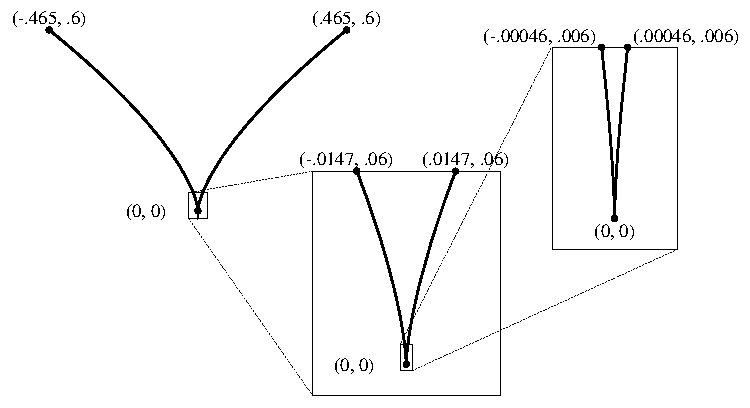
\includegraphics{../ps/calc1/cusp3.pdf}
  \newpage \thispagestyle{empty}

\mbox{}
\vspace{80pt}


\noindent
\textbf{Advisory Committee of the Five College Calculus Project}

\bigskip

\noindent
\begin{tabular}{l}
Peter Lax, \emph{Courant Institute, New York University}, Chairman \\
Solomon Garfunkel, \emph{COMAP, Inc.} \\
John Neuberger, \emph{The University of North Texas} \\
Barry Simon, \emph{California Institute of Technology} \\
Gilbert Strang, \emph{Massachusetts Institute of Technology} \\
John Truxal, \emph{State University of New York, Stony Brook}
\end{tabular}





%%%%%%%%%     front matter    %%%%%%%%%%%

% \newpage \setcounter{page}{1}\pagenumbering{roman}\chapter*{Preface: 2008 edition}

We are publishing this edition of \emph{Calculus in Context} online to
make it freely available to all users.  It is essentially unchanged
from the 1994 edition.

\medskip

The continuing support of Five Colleges, Inc., and especially of the
Five College Coordinator, Lorna Peterson, has been crucial in paving
the way for this new edition.  We also wish to thank the many
colleagues who have shared with us their experiences in using the book
over the last twenty years---and have provided us with corrections to
the text.


\chapter*{Preface: 1994 edition}

\paragraph{Our point of view}  
We believe that calculus can be for our students what it was for Euler
and the Bernoullis: A language and a tool for exploring the whole
fabric of science.  We also believe that much of the mathematical
depth and vitality of calculus lies in these connections to the other
sciences.  The mathematical questions that arise are compelling in
part because the answers matter to other disciplines as well.

The calculus curriculum that this book represents started with a
``clean slate;'' we made no presumptive commitment to any aspect of
the traditional course.  In developing the curriculum, we found it
helpful to spell out our {\bf starting points}, our {\bf curricular
  goals}, our {\bf functional goals}, and our view of the {\bf impact
  of technology}.  Our starting points are a summary of what calculus
is really about.  Our curricular goals are what we aim to convey about
the subject in the course.  Our functional goals describe the
attitudes and behaviors we hope our students will adopt in using
calculus to approach scientific and mathematical questions.  We
emphasize that what is missing from these lists is as significant as
what appears.  In particular, we did {\em not\/} not begin by asking
what parts of the traditional course to include or discard.

\medskip
\noindent
{\bf Starting Points}
\medskip

\begin{minipage}{343pt}

$\hspace{-12pt}\bullet$ Calculus is fundamentally a way of dealing
  with functional relationships that occur in scientific and
  mathematical contexts.  The techniques of calculus must be
  subordinate to an overall view of the underlying questions.

$\hspace{-12pt}\bullet$ Technology radically enlarges the range of
  questions we can explore and the ways we can answer them.  Computers
  and graphing calculators are much more than tools for teaching the
  traditional calculus.
\end{minipage}

\newpage

\noindent
{\bf Starting Points---continued}
\medskip

\begin{minipage}{343pt}
$\hspace{-12pt}\bullet$ The concept of a dynamical system is central
  to science Therefore, differential equations belong at the center of
  calculus, and technology makes this possible {\em at the
    introductory level}.

$\hspace{-12pt}\bullet$ The process of successive approximation is a
  key tool of calculus, even when the outcome of the process---the
  limit---cannot be explicitly given in closed form.
\end{minipage}

\bigskip
\noindent
{\bf Curricular Goals}
\medskip

\begin{minipage}{343pt}

$\hspace{-12pt}\bullet$ Develop calculus in the context of scientific
  and mathematical questions.

$\hspace{-12pt}\bullet$ Treat systems of differential equations as
  fundamental objects of study.

$\hspace{-12pt}\bullet$ Construct and analyze mathematical models.

$\hspace{-12pt}\bullet$ Use the method of successive approximations to
  define and solve problems.

$\hspace{-12pt}\bullet$ Develop geometric visualization with
  hand-drawn and computer graphics.

$\hspace{-12pt}\bullet$ Give numerical methods a more central role.
\end{minipage}

\bigskip
\noindent

\noindent
{\bf Functional Goals}
\medskip

\begin{minipage}{343pt}
$\hspace{-12pt}\bullet$ Encourage collaborative work.

$\hspace{-12pt}\bullet$ Empower students to use calculus as a language
  and a tool.

$\hspace{-12pt}\bullet$ Make students comfortable tackling large,
  messy, ill-defined problems.

$\hspace{-12pt}\bullet$ Foster an experimental attitude towards
  mathematics.

$\hspace{-12pt}\bullet$ Help students appreciate the value of
  approximate solutions.

$\hspace{-12pt}\bullet$ Develop the sense that understanding concepts
  arises out of working on problems, not simply from reading the text
  and imitating its techniques.
\end{minipage}

\medskip

\noindent
{\bf Impact of Technology}
\medskip

\begin{minipage}{343pt}
$\hspace{-12pt}\bullet$ Differential equations can now be solved
  numerically, so they can take their rightful place in the
  introductory calculus course.

$\hspace{-12pt}\bullet$ The ability to handle data and perform many
  computations allows us to explore examples containing more of the
  messiness of real problems.

$\hspace{-12pt}\bullet$ As a consequence, we can now deal with
  credible models, and the role of modelling becomes much more central
  to our subject.
\end{minipage}

\pagebreak

\noindent
{\bf Impact of Technology---continued}
\medskip

\begin{minipage}{343pt}
$\hspace{-12pt}\bullet$ In particular, introductory calculus (and
  linear algebra) now have something more substantial to offer to life
  and social scientists, as well as to physical scientists, engineers
  and mathematicians.

$\hspace{-12pt}\bullet$ The distinction between pure and applied
  mathematics becomes even less clear (or useful) than it may have
  been.
\end{minipage}

\bigskip
By studying the text you can see, quite explicitly, how we have
pursued the curricular goals.  In particular, every one of those goals
is addressed within the very first chapter.  It begins with questions
about describing and analyzing the spread of a contagious disease.  A
model is built, and the model is a system of coupled non-linear
differential equations.  We then begin a numerical assault on those
equations, and the door is opened to a solution by successive
approximations.

 Our implementation of the functional goals is less obvious, but it is
 still evident.  For instance, the text has many more words than the
 traditional calculus book---it is a book to be read.  Also, the
 exercises make unusual demands on students.  Most exercises are not
 just variants of examples that have been worked in the text.  In
 fact, the text has rather few simple ``template'' examples.

%\addtolength{\textheight}{20pt}

\paragraph{Shifts in Emphasis}  
It will also become apparent to you that the text reflects substantial
shifts in emphasis in comparison to the traditional course.  Here are
some of the most striking:
%\addtolength{\tabcolsep}{12pt}
\begin{center}
        \begin{tabular}{c@{\hspace{30pt}}c}
	\hline
        \multicolumn{2}{c}{\sc How the emphasis shifts:}\\ [2pt]
        {\sc increase} &  {\sc decrease} \\ [1pt]
        \hline \\ [-11pt]
        concepts        &  techniques \\ [1pt]
        geometry        &  algebra \\ [1pt]
        graphs          &  formulas \\ [1pt]
        brute force     &  elegance \\ [1pt]
        numerical       &  closed-form \\ [-3pt]
        solutions       &  solutions \\[2pt]
	\hline
        \end{tabular}
\end{center}

Euler's method is a good example of what we mean by ``brute force.''
It is a general method of wide applicability.  Of course when we use
it to solve a differential equation like $y'(t) = t$, we are using a
sledgehammer to crack a peanut.  But at least the sledgehammer {\em
  does\/} work.  Moreover, it works with coconuts (like $y' = y(1 -
y/10))$, and it will just as happily knock down a house (like $y' =
\cos^2(t))$.  Of course, students also see the elegant special methods
that can be invoked to solve $y' = t $ and $y' = y(1 - y/10)$
(separation of variables and partial fractions are discussed in
chapter 11), but they understand that they are fortunate indeed when a
real problem will succumb to these special methods.

\paragraph{Audience}  
Our curriculum is not aimed at a special clientele.  On the contrary,
we think that calculus is one of the great bonds that unifies science,
and all students should have an opportunity to see how the language
and tools of calculus help forge that bond.  We emphasize, though,
that this is not a ``service'' course or calculus ``with
applications,'' but rather a course rich in mathematical ideas that
will serve all students well, including mathematics majors.  The
student population in the first semester course is especially diverse.
In fact, since many students take only one semester, we have aimed to
make the first six chapters stand alone as a reasonably complete
course.  In particular, we have tried to present contexts that would
be more or less broadly accessible.  The emphasis on the physical
sciences is clearly greater in the later chapters; this is deliberate.
By the second semester, our students have gained skill and insight
that allows them to tackle this added complexity.

\paragraph{Handbook for Instructors}  
Working toward our curricular and functional goals has stretched us as
well as our students.  Teaching in this style is substantially
different from the calculus courses most of us have learned from and
taught in the past.  Therefore we have prepared a handbook based on
our experiences and those of colleagues at other schools.  We urge
prospective instructors to consult it.

\paragraph{Origins}  
The Five College Calculus Project has a singular history.  It begins
almost thirty years ago, when the Five Colleges were only Four:
Amherst, Mount Holyoke, Smith, and the large Amherst campus of the
University of Massachusetts.  These four resolved to create a new
institution which would be a site for educational innovation at the
undergraduate level; by 1970, Hampshire College was enrolling students
and enlisting faculty.

Early in their academic careers, Hampshire students grapple with
primary sources in all fields---in economics and ecology, as well as
in history and literature.  And journal articles don't shelter their
readers from home truths: if a mathematical argument is needed, it is
used.  In this way, students in the life and social sciences found,
sometimes to their surprise and dismay, that they needed to know
calculus if they were to master their chosen fields.  However, the
calculus they needed was not, by and large, the calculus that was
actually being taught.  The journal articles dealt directly with the
relation between quantities and their rates of change---in other
words, with differential equations.

Confronted with a clear need, those students asked for help.  By the
mid-1970s, Michael Sutherland and Kenneth Hoffman were teaching a
course for those students.  The core of the course was calculus, but
calculus as it is {\em used\/} in contemporary science.  Mathematical
ideas and techniques grew out of scientific questions.  Given a
process, students had to recast it as a model; most often, the model
was a set of differential equations.  To solve the differential
equations, they used numerical methods implemented on a computer.

The course evolved and prospered quietly at Hampshire.  More than a
decade passed before several of us at the other four institutions paid
some attention to it.  We liked its fundamental premise, that
differential equations belong at the center of calculus.  What
astounded us, though, was the revelation that differential equations
could really {\em be\/} at the center---thanks to the use of
computers.

This book is the result of our efforts to translate the Hampshire
course for a wider audience.  The typical student in calculus has not
been driven to study calculus in order to come to grips with his or
her own scientific questions---as those pioneering students had.  If
calculus is to emerge organically in the minds of the larger student
population, a way must be found to involve that population in a
spectrum of scientific and mathematical questions.  Hence, calculus
{\em in context}.  Moreover, those contexts must be understandable to
students with no special scientific training, and the mathematical
issues they raise must lead to the central ideas of the calculus---to
differential equations, in fact.

Coincidentally, the country turned its attention to the undergraduate
science curriculum, and it focused on the calculus course.  The
National Science Foundation created a program to support calculus
curriculum development.  To carry out our plans we requested funds for
a five-year project; we were fortunate to receive the only multi-year
curriculum development grant awarded in the first year of the NSF
program.  This text is the outcome of our effort.

%%%%%%%%%%%%%%%%%%%%%%%%%%%%%%%%%%%%%%%%%%%%%%%%%%%%%%%%%%%%%%%%%%%%%%%%

\section*{Acknowledgements}

Certainly this book would have been possible without the support of
the National Science Foundation and of Five Colleges, Inc.  We
particularly want to thank Louise Raphael who, as the first director
of the calculus program at the National Science Foundation, had faith
in us and recognized the value of what had already been accomplished
at Hampshire College when we began our work.  Five College
Coordinators Conn Nugent and Lorna Peterson supported and encouraged
our efforts, and Five College treasurer and business manager Jean
Stabell has assisted us in countless ways throughout the project.

We are very grateful to the members of our Advisory Board: to Peter
Lax, for his faith in us and his early help in organizing and chairing
the Board; to Solomon Garfunkel, for his advice on politics and
publishing; to Barry Simon, for using our text and giving us his
thoughtful and imaginative suggestions for improving it; to Gilbert
Strang, for his support of a radical venture; to John Truxal, for his
detailed commentaries and insights into the world of engineering.

Among our colleagues, James Henle of Smith College deserves special
thanks.  Besides his many contributions to our discussions of
curriculum and pedagogy, he developed the computer programs that have
been so valuable for our teaching: Graph, Slinky, Superslinky, and
Tint.  Jeff Gelbard and Fred Henle ably extended Jim's programs to the
MacIntosh and to DOS Windows and X Windows.  All of this software is
available on anonymous ftp at emmy.smith.edu.  Mark Peterson, Robert
Weaver, and David Cox also developed software that has been used by
our students.

Several of our colleagues made substantial contributions to our
frequent editorial conferences and helped with the writing of early
drafts.  We offer thanks to David Cohen, Robert Currier and James
Henle at Smith; David Kelly at Hampshire; and Frank Wattenberg at the
University of Massachusetts.  Mary Beck, who is now at the University
of Virginia, gave heaps of encouragement and good advice as a
co-teacher of the earliest version of the course at Smith.  Anne
Kaufmann, an Ada Comstock Scholar at Smith, assisted us with extensive
editorial reviews from the student perspective.

Two of the most significant new contributions to this edition are the
appendix for graphing calculators and a complete set of solutions to
all the exercises.  From the time he first became aware of our
project, Benjamin Levy has been telling us how easy and natural it
would be to adapt our Basic programs for graphing calculators.  He has
always used them when he taught {\em Calculus in Context}, and he
created the appendix which contains translations of our programs for
most of the graphing calculators in common use today.  Lisa Hodsdon,
Diane Jamrog, and Marcia Lazo have worked long hours over an entire
summer to solve all the exercises and to prepare the results as
\LaTeX{} documents for inclusion in the Handbook for Instructors.  We
think both these contributions do much to make the course more useful
to a wider audience.

We appreciate the contributions of our colleagues who participated in
numerous debriefing sessions at semester's end and gave us comments on
the evolving text.  We thank George Cobb, Giuliana Davidoff, Alan
Durfee, Janice Gifford, Mark Peterson, Margaret Robinson, and Robert
Weaver at Mount Holyoke; Michael Albertson, Ruth Haas, Mary Murphy,
Marjorie Senechal, Patricia Sipe, and Gerard Vinel at Smith.  We
learned, too, from the reactions of our colleagues in other
disciplines who participated in faculty workshops on Calculus in
Context.

We profited a great deal from the comments and reactions of early
users of the text.  We extend our thanks to Marian Barry at Aquinas
College, Peter Dolan and Mark Halsey at Bard College, Donald Goldberg
and his colleagues at Occidental College, Benjamin Levy at Beverly
High School, Joan Reinthaler at Sidwell Friends School, Keith Stroyan
at the University of Iowa, and Paul Zorn at St. Olaf College.  Later
users who have helped us are Judith Grabiner and Jim Hoste at Pitzer
College; Allen Killpatrick, Mary Scherer, and Janet Beery at the
University of Redlands; and Barry Simon at Caltech.

Dissemination grants from the NSF have funded regional workshops for
faculty planning to adopt Calculus in Context.  We are grateful to
Donald Goldberg, Marian Barry, Janet Beery, and to Henry Warchall of
the University of North Texas for coordinating workshops.

We owe a special debt to our students over the years, especially those
who assisted us in teaching, but also those who gave us the benefit of
their thoughtful reactions to the course and the text.  Seeing what
they were learning encouraged us at every step.
 
We continue to find it remarkable that our text is to be published the
way we want it, not softened or ground down under the pressure of
anonymous reviewers seeking a return to the mean.  All of this is due
to the bold and generous stance of W. H. Freeman.  Robert Biewen, its
president, understands---more than we could ever hope---what we are
trying to do, and he has given us his unstinting support.  Our
aquisitions editors, Jeremiah Lyons and Holly Hodder, have inspired us
with their passionate conviction that our book has something new and
valuable to offer science education.  Christine Hastings, our
production editor, has shown heroic patience and grace in shaping the
book itself against our often contrary views.  We thank them all.

%%%%%%%%%%%%%%%%%%%%%%%%%%%%%%%%%%%%%%%%%%%%%%%%%%%%%%%%%%%%%%%%%%%%%%%%%

\section*{To the Student}

In a typical high school math text, each section has a ``technique'' which you practice in a series of exercises very like the examples in the text.  This book is different.  In this course you will be learning to use calculus both as a tool and as a language in which you can think coherently about the problems you will be studying.  As with any other language, a certain amount of time will need to be spent learning and practicing the formal rules.  For instance, the conjugation of {\em \^etre\/} must be almost second nature to you if you are to be able to read a novel---or even a newspaper---in French.  In calculus, too, there are a number of manipulations which must become automatic so that you can focus clearly on the content of what is being said.  It is important to realize, however, that becoming good at these manipulations is not the goal of learning calculus any more than becoming good at declensions and conjugations is the goal of learning French.

Up to now, most of the problems you have met in math classes have had definite answers such as ``17,'' or ``the circle with radius 1.75 and center at (2,3).''  Such definite answers are satisfying (and even comforting).  However, many interesting and important questions, like ``How far is it to the planet Pluto,'' or ``How many people are there with sickle-cell anemia,'' or ``What are the solutions to the equation $x^5 + x + 1 = 0$'' can't be answered exactly.  Instead, we have ways to {\bf approximate} the answers, and the more time and/or money we are willing to expend, the better our approximations may be.  While many calculus problems do have exact answers, such problems often tend to be special or atypical in some way.  Therefore, while you will be learning how to deal with these ``nice'' problems, you will also be developing ways of making good approximations to the solutions of the less well-behaved (and more common!) problems.

The computer or the graphing calculator is a tool that that you will need for this course, along with a clear head and a willing hand.  We don't assume that you know anything about this technology ahead of time.  Everything necessary is covered completely as we go along.

You can't learn mathematics simply by reading or watching others.  The only way you can internalize the material is to work on problems yourself.  It is by grappling with the problems that you will come to see what it is you do understand, and to see where your understanding is incomplete or fuzzy.

One of the most important intellectual skills you can develop is that of exploring questions on your own.  Don't simply shut your mind down when you come to the end of an assigned problem.  These problems have been designed not so much to capture the essence of calculus as to prod your thinking, to get you wondering about the concepts being explored.  See if you can think up and answer variations on the problem.  Does the problem suggest other questions?  The ability to ask good questions of your own is at least as important as being able to answer questions posed by others.

We encourage you to work with others on the exercises.  Two or three of you of roughly equal ability working on a problem will often accomplish much more than would any of you working alone.  You will stimulate one another's imaginations, combine differing insights into a greater whole, and keep up each other's spirits in the frustrating times.  This is particularly effective if you first spend time individually working on the material.  Many students find it helpful to schedule a regular time to get together to work on problems.

 Above all, take time to pause and admire the beauty and power of what you are learning.  Aside from its utility, calculus is one of the most elegant and richly structured creations of the human mind and deserves to be profoundly admired on those grounds alone.  Enjoy!



% \tableofcontents \newpage \thispagestyle{empty}\mbox{}\newpage

%%%%%%%%%    chapters     %%%%%%%%%%%% 
  
\setcounter{page}{1}
\pagenumbering{arabic}

%%%%%%%%%%%%%%%%%%%%%%%%%%%%%%%%%%%%%%%%%%%%%%%%%%%%%%%%%%%%%%%%%%%%%
%                                                                   %
%                      Chapter 1 - Section 1                        %
%                                                                   %
%%%%%%%%%%%%%%%%%%%%%%%%%%%%%%%%%%%%%%%%%%%%%%%%%%%%%%%%%%%%%%%%%%%%% 

\chapter{A Context for Calculus}

Calculus gives us a language to describe how quantities are related to
one another, and it gives us a set of computational and visual tools
for exploring those relationships.  Usually, we want to understand how
quantities are related in the context of a particular problem---it
might be in chemistry, or public policy, or mathematics itself.  In
this chapter we take a single context---an infectious disease
spreading through a population---to see how calculus emerges and how
it is used.


\section{The Spread of Disease}

\subsection{Making a Model}

Many human diseases are contagious: you ``catch'' them from someone
who is already infected.  Contagious diseases are of many kinds.
Smallpox, polio, and plague are severe and even fatal, 
%
\mar{Some properties of contagious diseases} 
%
while the common cold and the childhood illnesses of measles, mumps,
and rubella are usually relatively mild.  Moreover, you can catch a
cold over and over again, but you get measles only once.  A disease
like measles is said to ``confer immunity'' on someone who recovers
from it.  Some diseases have the potential to affect large segments of
a population; they are called {\em epidemics}\index{epidemic} (from
the Greek words {\em epi}, upon + {\em demos}, the people.) {\em
  Epidemiology\/}\index{epidemiology} is the scientific study of these
diseases.

An epidemic is a complicated matter, but the dangers posed by
contagion---and especially by the appearance of new and uncontrollable
diseases---compel us to learn as much as we can about the nature of
epidemics.  Mathematics offers a very special kind of help.  First, we
can try to draw out of the situation its essential features and
describe them mathematically.  This is calculus as {\em language}.  We
substitute an ``ideal'' mathematical world for the real one.
%
\mar{The idea of a mathematical model}
%

This is calculus as {\em tool}.  Any conclusion we reach about the
model can then be interpreted to tell us something about the reality.

To give you an idea how this process works, we'll build a model of an
epidemic.  Its basic purpose is to help us understand the way a
contagious disease spreads through a population---to the point where
we can even predict what fraction falls ill, and when.  Let's suppose
the disease we want to model is like measles.  In particular,
\begin{itemize}
 \item it is mild, so anyone who falls ill eventually recovers;
 \item it confers permanent immunity on every recovered victim.
\end{itemize}
In addition, we will assume that the affected population is large but
fixed in size and confined to a geographically well-defined region.
To have a concrete image, you can imagine the elementary school
population of a big city.

At any time, that population can be divided into three distinct
classes:
\begin{description}
 \item[Susceptible:]\index{susceptible} those who have never had the
   illness and can catch it;
 \item[Infected:]\index{infected} those who currently have the illness
   and are contagious;
 \item[Recovered:]\index{recovered} those who have already had the
   illness and are immune.
\end{description}

Suppose we let $S$, $I$, and $R$ 
%
\mar{The quantities that our model analyzes}
%
denote the number of people in each of these three classes,
respectively.  Of course, the classes are all mixed together
throughout the population: on a given day, we may find persons who are
susceptible, infected, and recovered in the same family.  For the
purpose of organizing our thinking, though, we'll represent the whole
population as separated into three ``compartments'' as in the
following diagram:\index{compartment diagram}

\setlength{\unitlength}{1.5pt}
\begin{picture}(180,110)(-109,-55)
	\bezier{150}(-30,18)(0,68)(30,18) %150
	\bezier{150}(30,18)(62,-35)(0,-35) %150
	\bezier{150}(0,-35)(-62,-35)(-30,18) %150
	\put(0,0){\line(5,3){30}}
	\put(0,0){\line(-5,3){30}}
	\put(0,0){\line(0,-1){35}}
	\put(0,20){\makebox[0pt]{$S$}}
	\put(20,-12){\makebox[0pt]{$I$}}
	\put(-20,-12){\makebox[0pt]{$R$}}
	\put(0,48){\makebox[0pt]{Susceptible}}
	\put(46,-20){Infected}
	\put(-80,-20){Recovered}
	\put(0,-45){\makebox[0pt]{The Whole Population}}
\end{picture}

The goal of our model is to determine what happens to the numbers $S$,
$I$, and $R$ over the course of time.  Let's first see what our
knowledge and experience of childhood diseases might lead us to
expect.  When we say there is a ``measles outbreak,'' we mean that
there is a relatively sudden increase in the number of cases, and then
a gradual decline.  After some weeks or months, the illness virtually
disappears.  In other words, the number $I$ is a {\bf
  variable};\index{variable} its value changes over time.  One
possible way that $I$ might vary is shown in the following
graph.\index{graph}\label{Sgraph}


\setlength{\unitlength}{1pt}
\begin{picture}(340,140)(15,0)
	\put(50,20){\vector(1,0){255}}
	\put(50,20){\vector(0,1){100}}
	\put(290,8){time}
	\put(39,114){$I$}
	\begin{thicklines}
		\bezier{75}(50,25)(65,35)(75,60)
		\bezier{100}(75,60)(99,120)(124,72) %100
		\bezier{200}(124,72)(149,24)(300,23) %200
	\end{thicklines}
\end{picture}

During the course of the epidemic, susceptibles are constantly falling
ill.  Thus we would expect the number $S$ to show a steady decline.
Unless we know more about the illness, we cannot decide whether
everyone eventually catches it.  In graphical terms, this means we
don't know whether the graph of $S$ levels off at zero or at a value
above zero.  Finally, we would expect more and more people in the
recovered group as time passes.  The graph of $R$ should therefore
climb from left to right.  The graphs of $S$ and $R$ might take the
following forms:


\begin{picture}(340,140)(15,0)
	\put(50,20){\vector(1,0){255}}
	\put(50,20){\vector(0,1){100}}
	\put(290,8){time}
	\put(38,114){$S$}
	\begin{thicklines}
	\bezier{80}(50,100)(70,94)(100,71)
	\bezier{200}(100,71)(160,25)(300,24) %200
	\end{thicklines}
\end{picture}


\begin{picture}(340,140)(15,0)
	\put(50,20){\vector(1,0){255}}
	\put(50,20){\vector(0,1){100}}
	\put(290,8){time}
	\put(37,114){$R$}
	\begin{thicklines}
	\bezier{80}(50,30)(90,40)(120,70)
	\bezier{200}(120,70)(160,110)(300,110) %200
	\end{thicklines}
\end{picture}
\label{Rgraph}

While these graphs give us an idea about what might happen, they raise
some new questions, too.  For example, because there are no scales
marked along the axes,
%
\mar{Some quantitative questions that the graphs raise}
%
the first graph does not tell us how large $I$ becomes when the
infection reaches its peak, nor when that peak occurs.  Likewise, the
second and third graphs do not say how rapidly the population either
falls ill or recovers.  A good model of the epidemic should give us
graphs like these and it should also answer the quantitative questions
we have already raised---for example: When does the infection hit its
peak?  How many susceptibles eventually fall ill?


\subsection{A Simple Model for Predicting Change}

Suppose\label{`modelstart'} we know the values of $S$, $I$, and $R$
today; can we figure out what they will be tomorrow, or the next day,
or a week or a month from now?  Basically, this is a problem of
predicting the future.  One way to deal with it is to get an idea how
$S$, $I$, and $R$ are {\em changing}.  To start with a very simple
example, suppose the city's Board of Health reports that the measles
infection has been spreading at the rate of 470 new cases per day for
the last several days.  If that rate continues to hold steady and we
start with 20,000 susceptible children, then we can expect 470 fewer
susceptibles with each passing day.  The immediate future would then
look like this:
\begin{center}
\begin{tabular}{ccc}
			& accumulated		& remaining \\ [-2pt]
	days after& number of new	& number of \\ [-2pt]
	today	& infections		& susceptibles \\[2pt] 
		\hline 
	\begin{tabular}{c} \rule{0pt}{15pt} 0 \rule{0pt}{15pt} 
		\\ 1 \\ 2 \\ 3 \end{tabular} &
	\begin{tabular}{r} \rule{0pt}{15pt} 0 \\ 470 \\ 940 \\
		$1410$ \end{tabular}	&
	\begin{tabular}{r} \rule{0pt}{15pt}$20\,000$\\$19\,530$
	 \\ 	$19\,060$ \\ $18\,590$ \end{tabular} \\[-3pt]
	\vdots	&	\vdots		&	\vdots
\end{tabular}
\end{center}

Of course, these numbers will be correct only if the infection
continues to spread at its present rate of 470 persons per day.
%
\mar{Knowing rates, we can predict future values}  
%
If we want to follow $S$, $I$, and $R$ into the future, our example
suggests that we should pay attention to the {\bf
  rates}\index{rate}\index{rate of change} at which these quantities
change.  To make it easier to refer to them, let's denote the three
rates by $S'$, $I'$, and $R'$.  For example, in the illustration
above, $S$ is changing at the rate $S' = -470$ persons per day.  We
use a minus sign here because $S$ is {\em decreasing\/} over time.  If
$S'$ stays fixed we can express the value of $S$ after $t$ days by the
following formula:
\[
S = 20000 + S' \cdot t = 20000 - 470\,t \mbox{ persons.}
\] 
Check that this gives the values of $S$ found in the table when $t =
0$, 1, 2, or 3.  How many susceptibles does it say are left after 10
days?

Our assumption that $S' = -470$ persons per day amounts to a
mathematical characterization
%
\mar{The equation $S' = -470$ \\ is a model}
%
of the susceptible population---in other words, a model!  Of course it
is quite simple, but it led to a formula that told us what value we
could expect $S$ to have at any time $t$.

The model will even take us backwards in time\label{backwards}.  For
example, two days ago the value of $t$ was $-2$; according to the
model, there were
\[
S = 20000 - 470 \times -2 = 20940
\]
susceptible children then.  There is an obvious difference between
going backwards in time and going forwards: we already know the past.
Therefore, by letting $t$ be negative we can generate values for $S$
that can be checked against health records.  If the model gives good
agreement with {\em known\/} values of $S$ we become more confident in
using it to predict {\em future\/} values.

To predict the value of $S$ using the rate $S'$ we clearly need to
have a starting point---a known value of $S$
%
\mar{Predictions depend on the initial value, too}
%
from which we can measure changes.  In our case that starting point is
$S = 20000$.  This is called the {\bf initial value}\index{initial value} 
of $S$, because it is given to us at the ``initial time'' $t
= 0$.  To construct the formula $S = 20000 - 470\,t$, we needed to
have an initial value as well as a rate of change for $S$.

\smallskip

In the following pages we will develop a more complex model for all
three population groups that has the same general design as this
simple one.  Specifically, the model will give us information about
the rates $S'$, $I'$, and $R'$, and with that information we will be
able to predict the values of $S$, $I$, and $R$ at any time
$t$\label{`modelend'}.


\subsection{The Rate of Recovery}
\index{rate!of recovery}
\index{recovery}

Our first task will be to model the recovery rate $R'$.  We look at
the process of recovering first, because it's simpler to analyze.  An
individual caught in the epidemic first falls ill and then
recovers---recovery is just a matter of time.  In particular, someone
who catches measles\index{measles} has the infection for about
fourteen days.  So if we look at the entire infected population today,
we can expect to find some who have been infected less than one day,
some who have been infected between one and two days, and so on, up to
fourteen days.  Those in the last group will recover today.  In the
absence of any definite information about the fourteen groups, let's
assume they are the same size.  Then 1/14-th of the infected
population will recover today:
\[
\mbox{today the change in the recovered population} = 
          \dfrac{I \mbox{ persons}}{14 \mbox{ days}}.
\]
There is nothing special about today, though; $I$ has a value at any
time.  Thus we can make the same argument about any other day:
\[
\mbox{every day the change in the recovered population} 
		= \dfrac{I \mbox{ persons}}{14 \mbox{ days}}.
\]
This equation is telling us about $R'$, the rate at which $R$ is
changing.  We can write it more simply in the form
%
\mar{\vspace{.2in} The first piece of the $S$-$I$-$R$ model}
%
\[
R' = \dfrac{1}{14}I \mbox{ persons per day} .
\]

\newpage

We call this a {\bf rate equation}.\index{rate equation} Like any
equation, it links different quantities together.  In this case, it
links $R'$ to $I$.  The rate equation for $R$ is the first part of our
model of the measles epidemic.

\aside{Are you uneasy about our claim that {1/14-th} of the infected
  population recovers every day?  You have good reason to be.  After
  all, during the first few days of the epidemic almost no one has had
  measles the full fourteen days, so the recovery rate will be much
  less than $I/14$ persons per day.  About a week before the infection
  disappears altogether there will be no one in the early stages of
  the illness.  The recovery rate will then be much greater than
  $I/14$ persons per day.  Evidently our model is not a perfect mirror
  of reality!

\quad \ Don't be particularly surprised or dismayed by this.  Our goal
is to gain insight into the workings of an epidemic and to suggest how
we might intervene to reduce its effects.  So we start off with a
model which, while imperfect, still captures some of the workings.
The simplifications in the model will be justified if we are led to
inferences which help us understand how an epidemic works and how we
can deal with it.  If we wish, we can then refine the model, replacing
the simple expressions with others that mirror the reality more
fully.}

Notice that the rate equation for $R'$ does indeed give us a tool to
predict future values of $R$.  For suppose today 2100 people are
infected and 2500 have already recovered.  Can we say how large the
recovered population will be tomorrow or the next day?  Since $I =
2100$,
\[
R' = \dfrac{1}{14} \times 2100 = 150 \mbox{ persons per day}\, .
\]
Thus 150 people will recover in a single day, and twice as many, or
300, will recover in two.  At this rate the recovered population will
number 2650 tomorrow and 2800\label{`future'} the next day.

These calculations assume that the rate $R'$ holds steady at 150
persons per day for the entire two days.  Since $R' = I/14$, this is
the same as assuming that $I$ holds steady at 2100 persons.  If
instead $I$ varies during the two days we would have to adjust the
value of $R'$ and, ultimately, the future values of $R$ as well.  In
fact, $I$ {\em does\/} vary over time.  We shall see this when we
analyze how the infection is transmitted.  Then, in chapter 2, we'll
see how to make the adjustments in the values of $R'$ that will permit
us to predict the value of $R$ in the model with as much accuracy as
we wish.

\medskip

\noindent {\bf Other diseases}.  What can we say about the recovery
rate for a contagious disease other than measles? If the period of
infection of the new illness is $k$ days, instead of 14, and if we
assume that 1/$k$ of the infected people recover each day, then the
new recovery rate is
\[
R' = \dfrac{I \mbox{ persons}}{k \mbox{ days}} = 
			\dfrac{1}{k}I  \mbox{ persons per day.}
\]
If we set $b = 1/k$ we can express the recovery rate equation in the
form
\[
R' = bI  \mbox{ persons per day.}
\]
The constant $b$ is called the {\bf recovery
  coefficient}\index{recovery!coefficient} in this context.

\smallskip
\noindent
\begin{minipage}[b]{1.1in}
%\setlength{\unitlength}{1.5pt}
\begin{picture}(110,70)(-12,-30)
	\bezier{200}(-30,39)(0,89)(30,39) %200
	\put(0,21){\line(5,3){30}}
	\put(0,21){\line(-5,3){30}}
	\put(0,41){\makebox[0pt]{\footnotesize $S$}}

	\bezier{200}(42,18)(74,-35)(12,-35) %200
	\put(12,0){\line(5,3){30}}
	\put(12,0){\line(0,-1){35}}
	\put(32,-12){\makebox[0pt]{\footnotesize $I$}}

	\bezier{200}(-12,-35)(-74,-35)(-42,18) %200
	\put(-12,0){\line(-5,3){30}}
	\put(-12,0){\line(0,-1){35}}
	\put(-32,-12){\makebox[0pt]{\footnotesize $R$}}

%	\put(-11,-18){\line(1,1){9}}
%	\put(-11,-18){\line(1,-1){9}}
%	\multiput(-11,-18)(.3,.3){30}{\circle*{.1}}
%	\multiput(-11,-18)(.3,-.3){30}{\circle*{.2}}
	\bezier{30}(-11,-18)(-6.5,-13.5)(-2,-9)
	\bezier{30}(-11,-18)(-6.5,-22.5)(-2,-27)
	\put(-2,-11){\line(0,1){2}}
	\put(-2,-11){\line(1,0){12}}
	\put(-2,-25){\line(0,-1){2}}
	\put(-2,-25){\line(1,0){12}}
	\put(10,-11){\line(0,-1){14}}
	\put(0,-21){\makebox[0pt]{\footnotesize $b$}}
	\put(0,-45){\makebox[0pt]{\footnotesize recovery}}
\end{picture}
\setlength{\unitlength}{1pt}
\end{minipage} \hfill
\begin{minipage}[b]{3.8in}
\quad\ Let's incorporate our understanding of recovery into the
compartment diagram.  For the sake of illustration, we'll separate the
three compartments.  As time passes, people ``flow'' from the infected
compartment to the recovered.  We represent this flow by an arrow from
$I$ to $R$.  We label the arrow with the recovery coefficient $b$ to
indicate that the flow is governed by the rate equation $R' = b I$.
\end{minipage}


\subsection{The Rate of Transmission}
\index{rate!of transmission}
\index{transmission}

Since susceptibles become infected, the compartment diagram above
should also have an arrow that goes from $S$ to $I$ and a rate
equation for $S'$ to show how $S$ changes as the infection spreads.
While $R'$ depends only on $I$, because recovery involves only waiting
for people to leave the infected population, $S'$ will depend on both
$S$ and $I$, because transmission involves contact between susceptible
and infected persons.

Here's a way to model the transmission rate.  First, consider a single
susceptible person on a single day.  On average, this person will
contact only a small fraction, $p$, of the infected population.  For
example, suppose there are 5000 infected children, so $I = 5000$.  We
might expect only a couple of them---let's say 2---will be in the same
classroom with our ``average'' susceptible.  So the fraction of
contacts is $p = 2/I = 2/5000 = .0004$.  The 2 contacts themselves can
be expressed as $2 = (2/I)\cdot I = pI$ contacts per day per
susceptible.

To find out how many daily contacts the {\em whole\/} 
%
\mar{Contacts are proportional to both $S$ and $I$}
%
susceptible population will have, we can just multiply the average
number of contacts per susceptible person by the number of
susceptibles: this is $pI \cdot S = pSI$.

Not all contacts lead to new infections; only a certain fraction $q$
do.  The more contagious the disease, the larger $q$ is.  Since the
number of daily contacts is $pSI$, we can expect $q \cdot pSI$ new
infections per day (i.e., to convert contacts to infections, multiply
by $q$).  This becomes $aSI$ if we define $a$ to be the product $qp$.

Recall, the value of the recovery coefficient $b$ depends only on the
illness involved.  It is the same for all populations.  By contrast,
the value of $a$ depends on the general health of a population and the
level of social interaction between its members.  Thus, when two
different populations experience the same illness, the values of $a$
could be different.  One strategy for dealing with an epidemic is to
alter the value of $a$.  Quarantine\index{quarantine} does this, for
instance; see the exercises.

Since each new infection decreases the number of susceptibles, we have
the rate equation for $S$: 
%
\mar{\vspace{4pt} Here is the second piece of the $S$-$I$-$R$ model}
%
\[
S' =  - a S I \mbox{ persons per day} \, .
\]
The minus sign here tells us that $S$ is decreasing (since $S$ and $I$
are positive).  We call $a$ the {\bf transmission
  coefficient}.\index{transmission!coefficient}

\smallskip
\noindent
\begin{minipage}[b]{3.8in}
\quad\ Just as people flow from the infected to the recovered
compartment when they recover, they flow from the susceptible to the
infected when they fall ill.  To indicate the second flow let's add
another arrow to the compartment diagram.
\index{compartment diagram}\label{`diagram'} Because this flow is due to the
transmission of the illness, we will label the arrow with the
transmission coefficient $a$.  The compartment diagram now reflects
all aspects of our model.
\end{minipage}
\begin{minipage}[b]{1.1in}
\begin{picture}(110,70)(-74,-30)
	\bezier{200}(-30,39)(0,89)(30,39) %200
	\put(0,21){\line(5,3){30}}
	\put(0,21){\line(-5,3){30}}
	\put(0,41){\makebox[0pt]{\footnotesize $S$}}

	\put(27,10){\line(-4,1){12}}
	\put(27,10){\line(1,4){3}}
	\put(10,24){\line(3,-5){6}}
	\put(10,24){\line(5,3){12}}
	\put(22,31.2){\line(3,-5){6}}
	\put(21,18){\makebox[0pt]{\footnotesize $a$}}
	\put(37,25){\footnotesize transmission}

	\bezier{200}(42,18)(74,-35)(12,-35) %200
	\put(12,0){\line(5,3){30}}
	\put(12,0){\line(0,-1){35}}
	\put(32,-12){\makebox[0pt]{\footnotesize $I$}}

	\bezier{200}(-12,-35)(-74,-35)(-42,18) %200
	\put(-12,0){\line(-5,3){30}}
	\put(-12,0){\line(0,-1){35}}
	\put(-32,-12){\makebox[0pt]{\footnotesize $R$}}

	\bezier{30}(-11,-18)(-6.5,-13.5)(-2,-9)
	\bezier{30}(-11,-18)(-6.5,-22.5)(-2,-27)
	\put(-2,-11){\line(0,1){2}}
	\put(-2,-11){\line(1,0){12}}
	\put(-2,-25){\line(0,-1){2}}
	\put(-2,-25){\line(1,0){12}}
	\put(10,-11){\line(0,-1){14}}
	\put(0,-21){\makebox[0pt]{\footnotesize $b$}}
	\put(0,-45){\makebox[0pt]{\footnotesize recovery}}
\end{picture}
\setlength{\unitlength}{1pt}
\end{minipage}

\aside{We haven't talked about the units in which to measure $a$ and
  $b$.  They must be chosen so that any equation in which $a$ or $b$
  appears will balance.  Thus, in $R' = bI$ the units on the left are
  persons/day; since the units for $I$ are persons, the units for $b$
  must be 1/(days).  The units in $S' = -aSI$ will balance only if $a$
  is measured in 1/(person-day).

\quad\ The reciprocals have more natural interpretations.  First of
all, 1/$b$ is the number of days a person needs to recover.  Next,
note that 1/$a$ is measured in person-days (i.e., persons $\times$
days), which are the natural units in which to measure exposure.  Here
is why.  Suppose you contact 3~infected persons for each of 4~days.
That gives you the same exposure to the illness that you get from
6~infected persons in 2~days---both give 12 ``person-days'' of
exposure.  Thus, we can interpret $1/a$ as the level of exposure of a
typical susceptible person.}


\subsection{Completing the Model}

The final rate equation we need---the one for $I'$---reflects what is
already clear from the compartment diagram: every loss in $I$ is due
to a gain in $R$, while every gain in $I$ is due to a loss in $S$.

\newpage

\mbox{}\vspace{-12pt}
%
\mar{\vspace{10pt} Here is the complete $S$-$I$-$R$ model}
%
\begin{alignat*}{2}
		S' &=  -a S I,           &    &     \\
		I' &=  \hphantom{-}a S I &-\, & b I,  \\
		R' &=                    &    & b I.
\end{alignat*}
If you add up these three rates you should get the overall rate of
change of the whole population.  The sum is zero.  Do you see why?

\aside{You should not draw the conclusion that the only use of rate
  equations\index{rate equation} is to model an epidemic.  Rate
  equations have a long history, and they have been put to many uses.
  Isaac Newton\index{Newton, I.} (1642--1727) introduced them to model
  the motion of a planet around the sun.  He showed that the same rate
  equations could model the motion of the moon around the earth and
  the motion of an object falling to the ground.  Newton created
  calculus as a tool to analyze these equations.  He did the work
  while he was still an undergraduate---on an extended vacation,
  curiously enough, because a plague epidemic was raging at Cambridge!

\quad\ Today we use Newton's rate equations to control the motion of
earth satellites and the spacecraft that have visited the moon and the
planets.  We use other rate equations to model radioactive decay,
chemical reactions, the growth and decline of populations, the flow of
electricity in a circuit, the change in air pressure with
altitude---just to give a few examples.  You will have an opportunity
in the following chapters to see how they arise in many different
contexts, and how they can be analyzed using the tools of calculus.}

The following diagram summarizes, in a schematic way, the relation
between our model\index{model} and the reality it seeks to portray.

\begin{picture}(340,90)(10,-15)
	\put(-10,0)
	{
	\begin{picture}(120,70)
		\put(0,0){\framebox(120,50)
			{\shortstack{people fall ill\\[-2pt]
				and eventually\\[1pt] recover}}}
		\put(60,57){\makebox[0pt]{\bf Reality}}
	\end{picture}
	}
	\put(230,0)
	{
	\begin{picture}(120,70)
		\put(0,0){\framebox(120,50)
			{\shortstack{$S' = -aSI$ \\$I' = aSI - bI$ \\
				$R' = bI$}}}
		\put(60,57){\makebox[0pt]{\bf Mathematics}}
	\end{picture}
	}
	\put(125,32){\vector(1,0){90}}
	\put(215,18){\vector(-1,0){90}}
	\put(170,40){\makebox(0,0)[b]{\shortstack
		{Modelling \\ [-1pt] the reality}}}
	\put(170,13){\makebox(0,0)[t]{\shortstack
		{Interpreting \\ [-1pt] the mathematics}}}
\end{picture}


\noindent  
The diagram calls attention to several facts.  
%
\mar{The model is part of mathematics; it only approximates reality}
%
First, the model\index{model} is a part of mathematics.  It is
distinct from the reality being modelled.  Second, the model is based
on a simplified interpretation of the epidemic.  As such, it will not
match the reality exactly; it will be only an {\bf
  approximation}.\index{approximation} Thus, we cannot expect the
values of $S$, $I$, and $R$ that we calculate from the rate equations
to give us the exact sizes of the susceptible, infected, and recovered
populations.  Third, the connection between reality and mathematics is
a two-way street.  We have already travelled one way by constructing a
mathematical object that reflects some aspects of the epidemic.  This
is model-building.  Presently we will travel the other way.  First we
need to get mathematical answers to mathematical questions; then we
will see what those answers tell us about the epidemic.  This is
interpretation of the model.  Before we begin the interpretation, we
must do some mathematics.


\subsection{Analyzing the Model}

Now that we have a model\label{`analyzestart'} we shall analyze it as
a mathematical object.  We will set aside, at least for the moment,
the connection between the mathematics and the reality.  Thus, for
example, you should not be concerned when our calculations produce a
value for $S$ of 44,446.6 persons at a certain time---a value that
will never be attained in reality.  In the following analysis $S$ is
just a numerical quantity that varies with $t$, another numerical
quantity.  Using only mathematical tools we must now extract from the
rate equations the information that will tell us just how $S$ and $I$
and $R$ vary with $t$.

We already took the first steps in that direction when we used the
rate equation $R' = I/14$ to predict the value of $R$ two days into
the future (see page~\pageref{`future'}).  We assumed that $I$
remained fixed at 2100 during those two days, so the rate $R' =
2100/14 = 150$ was also fixed.  We concluded that if $R = 2500$ today,
it will be 2650 tomorrow and 2800 the next day.

A glance at the full $S$-$I$-$R$ model tells us those first steps have
to be modified.  The assumption
%
\mar{Rates are continually changing; this affects the calculations}
%
we made---that $I$ remains fixed---is not justified, because $I$ (like
$S$ and $R$) is continually changing.  As we shall see, $I$ actually
increases over those two days.  Hence, over the same two days, $R'$ is
not fixed at 150, but is continually increasing also.  That means that
$R'$ becomes larger than 150 during the first day, so $R$ will be
larger than $2650$ tomorrow.

The fact that the rates are continually changing complicates the
mathematical work we need to do to find $S$, $I$, and $R$.  In chapter
2 we will develop tools and concepts that will overcome this problem.
For the present we'll assume that the rates $S'$, $I'$, and $R'$ stay
fixed for the course of an entire day.  This will still allow us to
produce reasonable estimates\index{estimate} for the values of $S$,
$I$, and $R$.  With these estimates we will get our first glimpse of
the predictive power of the $S$-$I$-$R$ model.  We will also use the
estimates as the starting point for the work in chapter 2 that will
give us precise values.  Let's look at the details of a specific
problem.

\medskip

\noindent 
{\bf The Problem}.  Consider a measles epidemic in a school population
of 50,000 children.  The recovery coefficient is $b = 1/14$.  For the
transmission coefficient we choose $a = .00001$, a number within the
range used in epidemic studies.  We suppose that 2100 people are
currently infected and 2500 have already recovered.  Since the total
population is 50,000, there must be 45,400 susceptibles.  Here is a
summary of the problem in mathematical terms:
\begin{center}
\begin{picture}(360,140)
	\put(0,0){\framebox(360,140)
	{\begin{minipage}{4in}
	Rate equations:
	\vspace{-6pt}
	\begin{align*}
		S' &= -.00001SI,	\\
		I' &= .00001SI - I/14, \\
		R' &= I/14.	
		\end{align*}
	Initial values: when $t = 0$,
	\vspace{-6pt}
		$$
	S = 45400, \qquad I = 2100, \qquad R = 2500.
		$$
	\end{minipage}}}
\end{picture}
\end{center}

\smallskip

\noindent {\bf Tomorrow}.  From our earlier discussion, $R' = 2100/14
= 150$ persons per day, giving us an estimated value of $R = 2650$
persons for tomorrow.  To estimate $S$ we use
\[
S' = - .00001\,SI = - .00001 \times 45400 \times 2100
		= -953.4 \ \mbox{persons/day.}
\]
Hence we estimate that tomorrow 
\[
S = 45400 - 953.4 = 44446.6 \ \mbox{persons.}
\]
Since $S + I + R = 50000$ and we have $S + R = 47096.6$ tomorrow, a
final subtraction gives us $I = 2903.4$ persons.  (Alternatively, we
could have used the rate equation for $I'$ to estimate $I$.)

The fractional values in the estimates for $S$ and $I$ remind us that
the $S$-$I$-$R$ model describes the behavior of the epidemic only
approximately.

\medskip

\noindent {\bf Several days hence}.  According to the model, we
estimate that tomorrow $S = 44446.6$, $I = 2903.4$, and $R = 2650$.
Therefore, from the new $I$ we get a new approximation for the value
of $R'$ tomorrow; it is
\[
R' = \dfrac{1}{14} I = \dfrac{1}{14} \times 2903.4 = 207.4 \ 
			\mbox{persons/day.}
\]
Hence, two days from now we estimate that $R$ will have the new value
$2650 + 207.4 = 2857.4$.  Now follow this pattern to get new
approximations for $S'$ and $I'$, and then use those to estimate the
values of $S$ and $I$ two days from now.

\newpage

The pattern of steps that just carried you from the first day to the
second will work just as well to carry you from the second to the
third.
%
\mar{Stop and do\\ the calculations}
%
Pause now and do all these calculations yourself.  See exercises 15
and 16 on page~\pageref{`measles'}.  If you round your calculated
values of $S$, $I$, and $R$ to the nearest tenth, they should agree
with those in the following table.
\begin{center}
Estimates for the first three days\label{`threeday'}
\smallskip

{\small {\tabcolsep 3pt
\begin{tabular}{ccccccc}
	$t$ & $S$ & $I$ & $R$ & $S'$ & $I'$ & $R'$ \\ [2pt]
		\hline
	\begin{tabular}{c} \rule{0pt}{15pt} 0 \rule{0pt}{15pt} 
		\\ 1 \\ 2 \\ 3 \end{tabular} &
	\begin{tabular}{r} 
		\rule{0pt}{15pt} $45\,400.0$ \\ $44\,446.6$ \\
 		$43\,156.1$ \\ $41\,435.7$ \end{tabular} &
	\begin{tabular}{r} 
		\rule{0pt}{15pt} $2100.0$ \\ $2903.4$ \\
		 $3986.5$ \\ $5422.$1 \end{tabular} &
	\begin{tabular}{r} 
		\rule{0pt}{15pt} $2500.0$ \\ $2650.0$ \\
 		$2857.4$ \\ $3142.1$ \end{tabular} &
	\begin{tabular}{r} 
		\rule{0pt}{15pt} $-953.4$ \\ $-1290.5$ \\ 
		$-1720.4$ \\ \mbox{} \end{tabular} &
	\begin{tabular}{r} 
		\rule{0pt}{15pt} 803.4 \\ $1083.1$ \\ 
	$1435.7$ \\\mbox{} \end{tabular} &
	\begin{tabular}{r} 
		\rule{0pt}{15pt} 150.0 \\ 207.4 \\ 284.7 \\ 
		\mbox{} \end{tabular} 
\end{tabular}
}}
\end{center}

\noindent
{\bf Yesterday}.  We already pointed out, on
page~\pageref{backwards}, that we can use our models to go {\em
  backwards\/} in time, too.  This is a valuable way to see how well
the model fits reality, because we can compare estimates that the
model generates with health records for the days in the recent past.

To find how $S$, $I$, and $R$ change when we go one day into the
future we multiplied the rates $S'$, $I'$, and $R'$ by a time step of
+1.  To find how they change when we go one day into the past we do
the same thing, except that we must now use a time step of --1.
According to the table above, the rates at time $t = 0$ (i.e., today)
are
\[
S' = -953.4, \qquad I' = 803.4, \qquad R' = 150.0.
\]
Therefore we estimate that, one day ago, 
\begin{alignat*}{2}
S &= 45400 + (-953.4 \times -1)\; &= 45400 + 953.4 
		&=  46353.4,\\
I &= 2100 + (803.4 \times -1)   &= \hphantom{0}2100 - 803.4 
		&= 1296.6,  \\
R &= 2500 + (150.0 \times -1)   &= \hphantom{0}2500 - 150.0 
		&= 2350.0.  
\end{alignat*}
Just as we would expect with a spreading infection, there are more
susceptibles yesterday than today, but fewer infected or recovered.
In the exercises for section~3 you will have an opportunity to continue
this process, tracing the epidemic many days into the past.  For
example, you will be able to go back and see when the infection
started---that is, find the day when the value of $I$ was only about~1.

\newpage

\noindent
{\bf There and back again}.\index{there and back
  again}\label{`thereback'}
%
\mar{Go forward a day\\ and then back again}
%
What happens when we start with tomorrow's values and use tomorrow's
rates to go back one day---back to today?  We should get $S = 45400$,
$I = 2100$, and $R = 2500$ once again, shouldn't we?  Tomorrow's
values are
\begin{xalignat*}{3}
S  &= 44446.6, &   I  &= 2903.4, &   R  &= 2650.0, \\ 
S' &= -1290.5, &   I' &= 1083.1, &   R' &= 207.4.
\end{xalignat*}
To go backwards one day we must use a time step of $-1$.  The
predicted values are thus
\begin{alignat*}{2}
S &= 44446.6 + (-1290.6 \times -1) & &= 45737.2,  \\
I &= 2903.4 + (1083.1 \times -1) & &= 1820.3, \\
R &= 2650.0 + (207.4 \times -1) && = 2442.6. 
\end{alignat*}
These are {\em not\/} the values that we had at the start, when $t =
0$.  In fact, it's worth noting the difference\label{`differences'}
between the original values and those produced by ``going there and
back again.''
\begin{center}
\begin{tabular}{cccc}
		& original & there and	& \\[-2pt]
		& value	& back again	& difference \\ [2pt] \hline
	\begin{tabular}{c}
	\rule{0pt}{15pt}  $S$ \rule{0pt}{15pt} \\ $I$ \\ $R$ 
	\end{tabular} 
	&
	\begin{tabular}{r}
	\rule{0pt}{15pt}  45400 \\ 2100 \\ 2500
	\end{tabular}
	&
	\begin{tabular}{r}
	\rule{0pt}{15pt}  45737.1 \\ 1820.3 \\ 2442.6
	\end{tabular}
	&
	\begin{tabular}{r}
	\rule{0pt}{15pt}  337.1 \\ --279.7 \\ --57.4
	\end{tabular}
\end{tabular}
\end{center}

Do you see why there are differences?  We went forward in time using
the rates that were current at $t = 0$, but when we returned we used
the rates that were current at $t = 1$.  Because these rates were
different, we didn't get back where we started.  These differences do
not point to a flaw in the model; the problem lies with the way we are
trying to extract information from the model.  As we have been making
estimates,\index{estimate}
%
\mar{The differences measure how rough an estimate is}
%
we have assumed that the rates don't change over the course of a whole
day.  We already know that's not true, so the values that we have been
getting are not exact.  What this test adds to our knowledge is a way
to measure just {\em how\/} inexact those values are---as we do in the
table above.

\enlargethispage*{10pt}
In chapter 2 we will solve the problem of rough estimates by
recalculating all the quantities ten times a day, a hundred times a
day, or even more.  When we do the computations with shorter and
shorter time steps we will be able to see how the estimates improve.
We will even be able to see how to get values that are mathematically
exact!\label{`analyzeend'}

\medskip

\noindent
{\bf Delta notation}.\index{delta notation} This work has given us
some insights about the way our model predicts future values of $S$,
$I$, and $R$.  The basic idea is very simple: {\em determine how $S$,
  $I$, and $R$ change}.  Because these changes play such an important
role in what we do, it is worth having a simple way to refer to them.
Here is the notation that we will use:
\begin{center}
$\Delta x$ stands for a {\bf change}\index{change} in the quantity $x$ 
\end{center}
The symbol ``$\Delta$'' is the Greek capital letter {\em delta\/}; it
corresponds to the Roman letter ``D'' and stands for {\bf difference}.

Delta notation gives us a way to refer to changes of all sorts.  For
example, in the table on page~\pageref{`threeday'}, between day 1 and
day 3 the quantities $t$ and $S$ change by
\begin{align*}
	\Delta t &= 2 \text{ days},	\\
	\Delta S &=  -3010.9 \text{ persons}.
\end{align*}
We sometimes refer to a change as a {\bf step}.  
%
\mar{$\Delta$ stands for a change, a difference, or a step}
%
For instance, in this example we can say there is a ``$t$ step'' of 2
days, and an ``$S$ step'' of $-3010.9$ persons.  In the calculations
that produced the table on page~\pageref{`threeday'} we ``stepped
into'' the future, a day at a time.  Finally, delta notation gives us
a concise and vivid way to describe the relation between rates and
changes.  For example, if $S$ changes at the constant rate $S'$, then
under a $t$ step of $\Delta t$, the value of $S$ changes by
\[
\Delta S = S' \cdot \Delta t.
\]

\medskip
\noindent
{\bf Using the computer as a tool}.  Suppose we wanted to find out
what happens to $S$, $I$, and $R$ after a month, or even a year.  We
need only repeat---30 times, or 365 times---the three rounds of
calculations we used to go three days into the future.  The
computations would take time, though.  The same is true if we wanted
to do ten or one hundred rounds of calculations per day---which is the
approach we'll take in chapter 2 to get more accurate values.  To save
our time and effort we will soon begin to use a computer to do the
repetitive calculations.

\enlargethispage*{10pt}
A computer does calculations by following a set of instructions called
a {\bf program}.\index{program} Of course, if we had to give a million
instructions to make the computer carry out a million steps, there
would be no savings in labor.  The trick is to write a program with
just a few instructions that can be repeated over and over again to do
all the calculations we want.  The usual way to do this is to arrange
the instructions in a {\bf loop}\index{loop}\label{`loop'}.  To give
you an idea what a loop is, we'll look at the $S$-$I$-$R$
calculations.  They form a loop.  We can see the loop by making a flow
chart.

{\bf The flow chart}.\index{flow chart} We'll start by writing down
the three steps that take us from one day to the next:


\begin{description}
\item[Step I] Given the current values of $S$, $I$, and $R$, we get
  current $S'$, $I'$, and $R'$ by using the rate equations
\begin{alignat*}{2}
		S' &= - a S I, &   &     \\
		I' &= \hphantom{-}a S I & -\, & b I,  \\
		R' &=          &   & b I.
\end{alignat*}
\item[Step II] Given the current values of $S'$, $I'$, and $R'$, we
  find the changes $\Delta S$, $\Delta I$, and $\Delta R$ over the
  course of a day by using the equations
\begin{align*}
\Delta S \mbox{ persons} &= S' \ \dfrac{\mbox{persons}}{\mbox{day}} 
          \times 1 \ \mbox{day}, \\[4pt]
\Delta I \mbox{ persons} &= I' \ \dfrac{\mbox{persons}}{\mbox{day}} 
          \times 1 \ \mbox{day}, \\[4pt]
\Delta R \mbox{ persons} &= R' \ \dfrac{\mbox{persons}}{\mbox{day}} 
          \times 1 \ \mbox{day}.
\end{align*}
\item[Step III] Given the current values of $\Delta S$, $\Delta I$,
  and $\Delta R$, we find the new values of $S$, $I$, and $R$ a day
  later by using the equations
\begin{align*}
	\mbox{new $S$} &= \mbox{current $S$} + \Delta S, \\
	\mbox{new $I$} &= \mbox{current $I$} + \Delta I, \\
	\mbox{new $R$} &= \mbox{current $R$} + \Delta R.
\end{align*}
\end{description}

\noindent
Each step takes three numbers as {\bf input},\index{input} and
produces three new numbers as {\bf output}.\index{output} Note that
the output of each step is the input of the next, so the steps flow
together.  The diagram below, called a {\bf flow chart},\index{flow
  chart} 
%
\mar{\vspace{40pt} The flow chart\\ forms a loop} 
%
shows us how the steps are connected.

\begin{picture}(340,110)(5,0)\label{`flowchart'}
\put(0,50)
	{\begin{picture}(80,50)
	\put(0,5){\framebox(80,40)
		{\shortstack{values of\\[2pt]$S$, $I$, $R$}}}
	\end{picture}}
\put(130,50)
	{\begin{picture}(80,50)
	\put(0,5){\framebox(80,40)
		{\shortstack{values of\\[2pt]$S'$, $I'$, $R'$}}}
	\end{picture}}
\put(260,50)
	{\begin{picture}(80,50)
	\put(0,5){\framebox(80,40)
		{\shortstack{values of\\[2pt]
			$\Delta S$, $\Delta I$, $\Delta R$}}}
	\end{picture}}
\put(90,75){\vector(1,0){30}}
\put(220,75){\vector(1,0){30}}
\put(300,15){\line(0,1){30}}
\put(40,15){\vector(0,1){30}}
\put(40,15){\line(1,0){260}}
\put(105,85){\makebox[0pt]{I}}
\put(235,85){\makebox[0pt]{II}}
\put(170,25){\makebox[0pt]{III}}
\end{picture}

\noindent The calculations form a {\bf loop}\index{loop}, because the
output of step III is the input for step I.  If we go once around the
loop, the output of step III gives us the values of $S$, $I$, and $R$
{\em on the following day}.  The steps do indeed carry us into the
future.

Each step involves calculating three numbers.  If we count each
calculation as a single instruction, then it takes nine instructions
to carry the values of $S$, $I$, and $R$ one day into the future.  To
go a million days into the future, we need add only one more
instruction: ``Go around the loop a million times.''  In this way, a
computer program with only ten instructions can carry out a million
rounds of calculations!

Later in this chapter (section~3) you will find a real computer
program that lists these instructions (for three days instead of a
million, though).
%
\mar{A computer program\\ will carry out\\ the three steps}
%
Study the program to see which instructions accomplish which steps.
In particular, see how it makes a loop.  Then run the program to check
that the computer reproduces the values you already computed by hand.
Once you see how the program works, you can modify it to get further
information---for example, you can find out what happens to $S$, $I$,
and $R$ thirty days into the future.  You will even be able to plot
the graphs of $S$, $I$, and $R$.

\aside{Rate equations\index{rate equation} have always been at the
  heart of calculus, and they have been analyzed using mechanical and
  electronic computers for as long as those tools have been available.
  Now that small powerful computers have begun to appear in the
  classroom, it is possible for beginning calculus students to explore
  interesting and complex problems that are modelled by rate
  equations.  Computers are changing how mathematics is done and how
  it is learned.}

\medskip

\noindent {\bf Analysis without a computer}.  A computer is a powerful
tool for exploring the $S$-$I$-$R$ model, but there are many things we
can learn about the model without using a computer.  Here is an
example.

According to the model, the rate at which the infected population
grows is given by the equation
\[
I' = .00001 \, S I - I/14 \quad \mbox{persons/day.}
\]
In our example, $I' = 803.4$ at the outset.  This is a positive
number, so $I$ increases initially.  In fact, $I$ will continue to
increase as long as $I'$ is positive.  If $I'$ ever becomes negative,
then $I$ decreases.  So let's ask the question: when is $I'$ positive,
when is it negative, and when is it zero?  By factoring out $I$ in the
last equation we obtain
\[
I' = I \left( .00001 \, S - \dfrac{1}{14} \right) \ \mbox{persons/day.}
\]
Consequently $I' = 0$ if either
\[
I = 0 \qquad \mbox{or} \qquad .00001 \, S - \dfrac{1}{14} = 0.
\]
The first possibility $I = 0$ has a simple interpretation: there is no
infection within the population.  The second possibility is more
interesting; it says that $I'$ will be zero when
\[
.00001 \, S - \dfrac{1}{14} = 0 \qquad \mbox{or} \qquad
		S = \dfrac{100000}{14} \approx 7142.9.
\]

If $S$ is {\em greater\/} than $100000/14$ and $I$ is positive, then
you can check that the formula
\[
I' = I \left( .00001 \, S - \dfrac{1}{14} \right) 
		\ \mbox{persons/day}
\]
tells us $I'$ is positive---so $I$ is increasing.  If, on the other
hand, $S$ is {\em less than\/} $100000/14$, then $I'$ is negative and
$I$ is decreasing.  So $S = 100000/14$ represents a {\bf
  threshold}.\index{threshold}\label{`threshold'} If $S$ falls below
the threshold, $I$ decreases.  If $S$ exceeds the threshold, $I$
increases.  Finally, $I$ reaches its peak when $S$ equals the
threshold.

The presence of a threshold value for $S$ is purely a  mathematical result.  However, it has an interesting interpretation for the epidemic.  
%
\mar{The threshold determines whether there will be an epidemic}
%
As long as there are at least $7143$ susceptibles, the infection will
spread, in the sense that there will be more people falling ill than
recovering each day.  As new people fall ill, the number of
susceptibles declines.  Finally, when there are fewer than $7143$
susceptibles, the pattern reverses: each day more people will recover
than will fall ill.

If there were fewer than $7143$ susceptibles in the population {\em at
  the outset}, then the number of infected would only decline with
each passing day.  The infection would simply never catch hold.  The
clear implication is that the noticeable surge in the number of cases
that we associate with an ``epidemic'' disease is due to the presence
of a large susceptible population.  If the susceptible population lies
below a certain threshold value, a surge just isn't possible.  This is
a valuable insight---and we got it with little effort.  We didn't need
to make lengthy calculations or call on the resources of a computer; a
bit of algebra was enough.

\newpage

\subsection{Exercises}

\subsubsection{Reading a Graph}

\index{graph} The graphs on pages \pageref{Sgraph}
and~\pageref{Rgraph} have no scales marked along their axes, so they
provide mainly {\em qualitative\/} information.  The graphs below do
have scales, so you can now answer {\em quantitative\/} questions
about them.  For example, on day 20 there are about 18,000 susceptible
people.  Read the graphs to answer the following questions.  (Note: $S
+ I + R$ is {\em not\/} constant in this example, so these graphs
cannot be solutions to our model..)

\setlength{\unitlength}{1pt}
%\begin{picture}(340,140)(15,0)
\begin{picture}(340,135)(15,0)
	\put(310,25){time}
	\put(56,114){$S$}
	\put(90,20){\line(0,1){90}}
	\put(130,20){\line(0,1){90}}
	\put(170,20){\line(0,1){90}}
	\put(210,20){\line(0,1){90}}
	\put(250,20){\line(0,1){90}}
	\put(90,8){\makebox[0pt]{10}}
	\put(130,8){\makebox[0pt]{20}}
	\put(170,8){\makebox[0pt]{30}}
	\put(210,8){\makebox[0pt]{40}}
	\put(250,8){\makebox[0pt]{50}}
	\put(290,8){days}
	\put(50,57){\line(1,0){230}}
	\put(50,94){\line(1,0){230}}
	\put(46,53){\makebox[0pt][r]{$20000$}}
	\put(46,90){\makebox[0pt][r]{$40000$}}
	\put(46,114){\makebox[0pt][r]{people}}
	\begin{thicklines}
	\put(50,20){\vector(1,0){255}}
	\put(50,20){\vector(0,1){100}}
	\bezier{75}(50,100)(70,94)(100,71)
	\bezier{50}(100,71)(160,25)(300,24) %200
	\end{thicklines}
\end{picture}

%\begin{picture}(340,140)(15,0)
\begin{picture}(340,130)(15,0)
	\put(310,25){time}
	\put(56,114){$I$}
	\put(90,20){\line(0,1){90}}
	\put(130,20){\line(0,1){90}}
	\put(170,20){\line(0,1){90}}
	\put(210,20){\line(0,1){90}}
	\put(250,20){\line(0,1){90}}
	\put(90,8){\makebox[0pt]{10}}
	\put(130,8){\makebox[0pt]{20}}
	\put(170,8){\makebox[0pt]{30}}
	\put(210,8){\makebox[0pt]{40}}
	\put(250,8){\makebox[0pt]{50}}
	\put(290,8){days}
	\put(50,47){\line(1,0){230}}
	\put(50,74){\line(1,0){230}}
	\put(50,101){\line(1,0){230}}
	\put(46,44){\makebox[0pt][r]{$5000$}}
	\put(46,71){\makebox[0pt][r]{$10000$}}
	\put(46,98){\makebox[0pt][r]{$15000$}}
	\put(46,116){\makebox[0pt][r]{people}}
	\begin{thicklines}
	\put(50,20){\vector(1,0){255}}
	\put(50,20){\vector(0,1){100}}
	\bezier{75}(50,25)(65,35)(75,60)
	\bezier{50}(75,60)(99,120)(124,72) %120
	\bezier{50}(124,72)(149,24)(300,23) %200
	\end{thicklines}
\end{picture}


%\begin{picture}(340,140)(15,0)
\begin{picture}(340,130)(15,0)
	\put(310,25){time}
	\put(56,120){$R$}
	\put(90,20){\line(0,1){90}}
	\put(130,20){\line(0,1){90}}
	\put(170,20){\line(0,1){90}}
	\put(210,20){\line(0,1){90}}
	\put(250,20){\line(0,1){90}}
	\put(90,8){\makebox[0pt]{20}}
	\put(130,8){\makebox[0pt]{40}}
	\put(170,8){\makebox[0pt]{60}}
	\put(210,8){\makebox[0pt]{80}}
	\put(250,8){\makebox[0pt]{100}}
	\put(290,8){days}
	\put(50,57){\line(1,0){230}}
	\put(50,94){\line(1,0){230}}
	\put(46,53){\makebox[0pt][r]{$20000$}}
	\put(46,90){\makebox[0pt][r]{$40000$}}
	\put(46,120){\makebox[0pt][r]{people}}
	\begin{thicklines}
	\put(50,20){\vector(1,0){255}}
	\put(50,20){\vector(0,1){100}}
	\bezier{90}(50,30)(90,40)(120,70)
	\bezier{50}(120,70)(160,110)(300,110) %200
	\end{thicklines}
\end{picture}

\vspace{-10pt} 

\enlargethispage*{10pt}
\num When does the infection hit its peak?\index{maximum} How many
people are infected at that time?

\num Initially, how many people are susceptible?  How many days does
it take for the susceptible population to be cut in half?

\num How many days does it take for the recovered population to reach
25,000?  How many people {\em eventually\/} recover?  Where did you
look to get this information?

\num On what day is the size of the infected population increasing
most rapidly?  When is it decreasing most rapidly?  How do you know?

\num How many people caught the illness at some time during the first
20 days?  (Note that this is not the same as the number of people who
are infected on day 20.)  Explain where you found this information.

\num Copy the graph of $R$ as accurately as you can, and then
superimpose a sketch of $S$ on it.  Notice the time scales on the {\em
  original\/} graphs of $S$ and $R$ are different.  Describe what
happened to the graph of $S$ when you superimposed it on the graph of
$R$.  Did it get compressed or stretched?  Was this change in the
horizontal direction or the vertical?

\subsubsection{A Simple Model}

These questions concern the rate equation $S' = -470$ persons per day
that we used to model a susceptible population on
pages \pageref{`modelstart'}--\pageref{`modelend'}.

\num Suppose the initial susceptible population was 20,000 on
Wednesday.  Use the model to answer the following questions.

\sub  How many susceptibles will be left ten days later?

\sub How many days will it take for the susceptible population to
vanish entirely?

\sub  How many susceptibles were there on the previous Sunday?  

\sub How many days before Wednesday were there 30,000 susceptibles?



\subsubsection{Mark Twain's Mississippi}
\index{Mississippi}

The Lower Mississippi River meanders over its flat valley, forming
broad loops called ox-bows.\index{ox-bow} In a flood, the river can
jump its banks and cut off one of these loops, getting shorter in the
process.  In his book {\em Life on the Mississippi} (1884), Mark
Twain\index{Twain, M.} suggests, with tongue in cheek, that some day
the river might even vanish!  Here is a passage that shows us some of
the pitfalls in using rates to predict the future and the past.
\begin{quote}\label{`twain'}
{\small In the space of one hundred and seventy six years the Lower
  Mississippi has shortened itself two hundred and forty-two miles.
  That is an average of a trifle over a mile and a third per year.
  Therefore, any calm person, who is not blind or idiotic, can see
  that in the Old O\"{o}litic Silurian Period, just a million years
  ago next November, the Lower Mississippi was upwards of one million
  three hundred thousand miles long, and stuck out over the Gulf of
  Mexico like a fishing-pole.  And by the same token any person can
  see that seven hundred and forty-two years from now the Lower
  Mississippi will be only a mile and three-quarters long, and Cairo
  [Illinois] and New Orleans will have joined their streets together
  and be plodding comfortably along under a single mayor and a mutual
  board of aldermen.  There is something fascinating about science.
  One gets such wholesome returns of conjecture out of such a trifling
  investment of fact.}
\end{quote}

\noindent  
Let $L$ be the length of the Lower Mississippi River.  Then $L$ is a
variable quantity we shall analyze.

\num According to Twain's data, what is the exact {\bf
  rate}\index{rate} at which $L$ is changing, in miles per year?  What
approximation does he use for this rate?  Is this a reasonable
approximation? Is this rate {\em positive\/} or {\em negative\/}?
Explain.  In what follows, use Twain's approximation.

\num Twain wrote his book in 1884.  Suppose the Mississippi that Twain
wrote about had been 1100 miles long; how long would it have become in
1990?

\num Twain does not tell us how long the Lower Mississippi was in 1884
when he wrote the book, but he does say that 742 years later it will
be only $1\tfrac{3}{4}$ miles long.  How long must the river have been
when he wrote the book?

\num Suppose $t$ is the number of years since 1884.  Write a formula
that describes how much $L$ has changed in $t$ years.  Your formula
should complete the equation
\[
\mbox{the change in $L$ in $t$ years} = \ldots \ . \rule{90pt}{0pt}
\]

\num From your answer to question 10, you know how long the river was
in 1884.  From question 11, you know how much the length has changed
$t$ years after 1884.  Now write a formula that describes how long the
river is $t$ years later.

\num Use your formula to find what $L$ was a million years ago.  Does
your answer confirm Twain's assertion that the river was ``upwards of
1,300,000 miles long'' then?

\num Was the river ever 1,300,000 miles long; will it ever be
$1\tfrac{3}{4}$ miles long?  (This is called a {\bf reality check}.)
What, if anything, is wrong with the ``trifling investment of fact''
which led to such ``wholesale returns of conjecture'' that Twain has
given us?


\subsubsection{The Measles Epidemic}

We consider once again the specific rate equations 
\begin{align*}
S' &= -.00001 \, SI, \\
I' &= .00001 \, SI - I/14, \\
R' &= I/14, 
\end{align*}
discussed in the text on pages
\pageref{`analyzestart'}--\pageref{`analyzeend'}.  We saw that at time
$t = 1$,
\[
S = 44446.6, \qquad I = 2903.4, \qquad R = 2650.0.
\]

\num Calculate the current rates of change $S'$, $I'$, and $R'$ when
$t = 1$, and then use these values to determine $S$, $I$, and $R$ one
day later\label{`measles'}.

\num In the previous question you found $S$, $I$, and $R$ when $t =
2$.  Using these values, calculate the rates $S'$, $I'$, and $R'$ and
then determine the new values of $S$, $I$, and $R$ when $t = 3$.  See
the table on page~\pageref{`threeday'}.

\num {\bf Double the time step}.  Go back to the starting time $t = 0$
and to the initial values
\[
S = 45400, \qquad I = 2100, \qquad R = 2500.
\]
Recalculate the values of $S$, $I$, and $R$ at time $t = 2$ by using a
time step of $\Delta t = 2$.  You should perform only a single round
of calculations, and use the rates $S'$, $I'$, and $R'$ that are
current at time $t = 0$.


\num {\bf There and back again}.\index{there and back
  again}\label{`therebackprob'} In the text we went one day into the
future and then back again to the present.  Here you'll go forward two
days from $t = 0$ and then back again.  There are two ways to do this:
with a time step of $\Delta t = \pm 2$ (as in the previous question),
and with a pair of time steps of $\Delta t = \pm 1$ .

\sub ($\Delta t = \pm 2$).  Using the values of $S$, $I$, and $R$ at
time $t = 2$ that you just got in the previous question, calculate the
rates $S'$, $I'$, and $R'$.  Then using a time step of $\Delta t =
-2$, estimate new values of $S$, $I$, and $R$ at time $t = 0$.  How
much do these new values differ from the original values 45,400, 2100,
2500?

\sub  ($\Delta t = \pm 1$).  Now make a new start, using the values 
\begin{xalignat*}{3}
S  &= 43156.1, &  I  &= 3986.5, &  R  &= 2857.4, \\ 
S' &= -1720.4, &  I' &= 1435.7, &  R' &= 284.7.
\end{xalignat*}
that occur when $t = 2$ if we make estimates with a time step $\Delta
t = 1$.  (These values come from the table on
page~\pageref{`threeday'}) Using two rounds of calculations with a
time step of $\Delta t = -1$, estimate another set of new values for
$S$, $I$, and $R$ at time $t = 0$.  How much do these new values
differ from the original values 45,400, 2100, 2500?

\sub Which process leads to a {\em smaller\/} set of differences: a
single round of calculations with $\Delta t = \pm 2$, or two rounds of
calculations with $\Delta t = \pm 1$?  Consequently, which process
produces better estimates---in the sense in which we used to measure
estimates on page~\pageref{`differences'}?


\num {\bf Quarantine}.\index{quarantine} One of the ways to treat an
epidemic is to keep the infected away from the susceptible; this is
called quarantine.  The intention is to reduce the chance that the
illness will be transmitted to a susceptible person.  Thus, quarantine
alters the {\em transmission coefficient}.

\sub Suppose a quarantine is put into effect that cuts in half the
chance that a susceptible will fall ill.  What is the new transmission
coefficient?

\sub On page~\pageref{`threshold'} it was determined that whenever
there were fewer than 7143 susceptibles, the number of infected would
decline instead of grow.  We called 7143 a {\em
  threshold\/}\index{threshold} level for $S$.  Changing the
transmission coefficient, as in part (a), changes the threshold level
for $S$.  What is the new threshold?

\sub Suppose we start with $S$ = 45,400.  Does quarantine eliminate
the epidemic, in the sense that the number of infected immediately
goes down from 2100, without ever showing an increase in the number of
cases?

\sub Since the new transmission coefficient is not small enough to
guarantee that $I$ never goes up, can you find a smaller value that
{\em does\/} guarantee $I$ never goes up?  Continue to assume we start
with $S = 45400$.

\sub Suppose the initial susceptible population is 45,400.  What is
the {\em largest\/} value that the transmission coefficient can have
and still guarantee that $I$ never goes up?  What level of quarantine
does this represent?  That is, do you have to reduce the chance that a
susceptible will fall ill to one-third of what it was with no
quarantine at all, to one-fourth, or what?


\subsubsection{Other Diseases}

\vspace{-10pt}

\num Suppose the spread of an illness similar to measles is modelled
by the following rate equations:
\begin{align*}
S' &= -.00002 \, SI, \\
I' &= .00002 \, SI - .08 \, I, \\
R' &= .08 \, I.
\end{align*}
Note: the initial values $S = 45400$, etc.\ that we used in the text
do not apply here.

\sub Roughly how long does someone who catches this illness remain
infected?  Explain your reasoning.

\sub How large does the susceptible population have to be in order for
the illness to take hold---that is, for the number of cases to
increase?  Explain your reasoning.

\sub Suppose 100 people in the population are currently ill.
According to the model, how many (of the 100 infected) will recover
during the next 24 hours?

\sub Suppose 30 {\em new\/} cases appear during the same 24 hours.
What does that tell us about $S'$?

\sub Using the information in parts (c) and (d), can you determine how
large the current susceptible population is?

\numa Construct the appropriate $S$-$I$-$R$ model for a measles-like
illness that lasts for 4 days.  It is also known that a typical
susceptible person meets only about 0.3\% of infected population each
day, and the infection is transmitted in only one contact out of six.

\sub How small does the susceptible population have to be for this
illness to fade away without becoming an epidemic?

\num Consider the general $S$-$I$-$R$ model for a measles-like
illness:
\begin{alignat*}{2}
S' &=  - a S I,         &     &     \\
I' &= \hphantom{-}a S I & -\, & b I,  \\
R' &=                   &     & b I.
\end{alignat*}

\sub The threshold level for $S$---below which the number of infected
will only decline---can be expressed in terms of the transmission
coefficient $a$ and the recovery coefficient $b$.  What is that
expression?\label{`setthresh'}

\sub Consider two illnesses with the same transmission coefficient
$a$; assume they differ only in the length of time someone stays ill.
Which one has the lower threshold level for $S$?  Explain your
reasoning.


\subsubsection{What Goes Around Comes Around}

Some relatively mild illnesses, like the common cold, return to infect
you again and again.  For a while, right after you recover from a
cold, you are immune.  But that doesn't last; after some weeks or
months, depending on the illness, you become susceptible again.  This
means there is now a flow from the recovered population to the
susceptible.  These exercises ask you to modify the basic $S$-$I$-$R$
model to describe an illness where immunity is temporary.

\num Draw a compartment diagram for such an illness.  Besides having
all the ingredients of the diagram on page~\pageref{`diagram'}, it
should depict a flow from $R$ to~$S$.  Call this {\bf immunity
  loss},\index{immunity loss} and use $c$ to denote the coefficient of
immunity loss.

\num Suppose immunity is lost after about six weeks.  Show that you
can set $c = 1/42$ per day, and explain your reasoning carefully.  A
suggestion: adapt the discussion of recovery in the text.

\num Suppose this illness lasts 5 days and it has a transmission
coefficient of .00004 in the population we are considering.  Suppose
furthermore that the total population is fixed in size (as was the
case in the text).  Write down rate equations for $S$, $I$, and $R$.

\num We saw in the text that the model for an illness that confers
permanent immunity has a threshold value for $S$ in the sense that
when $S$ is above the threshold, $I$ increases, but when it is below,
$I$ decreases.  Does {\em this\/} model have the same feature?  If so,
what is the threshold value?

\num For a mild illness that confers permanent immunity, the size of
the recovered population can only grow.  This question explores what
happens when immunity is only temporary.

\sub  Will $R$ increase or decrease if 
\[
S = 45400, \qquad I = 2100, \qquad R = 2500?
\]

\sub Suppose we shift 20000 susceptibles to the recovered population
(so that $S = 25400$ and $R = 22500$), leaving $I$ unchanged.  Now,
will $R$ increase or will it decrease?

\sub Using a total population of 50,000, give two other sets of values
for $S$, $I$, and $R$ that lead to a decreasing $R$.

\sub In fact, the relative sizes of $I$ and $R$ determine whether $R$
will increase or decrease.  Show that
\begin{align*}
\text{if } & I > \tfrac{5}{42} R, \quad 
		\text{then $R$ will increase;} \\
\text{if } & I < \tfrac{5}{42} R,  \quad
		\text{then $R$ will decrease.} 
\end{align*}
Explain your argument clearly.  A suggestion: consider the rate
equation for~$R'$.

\num {\bf The steady state}.  Any illness that confers only temporary
immunity can appear to linger in a population forever.  You may not
always have a cold, but someone does, and eventually you catch another
one.  (``What goes around comes around.'')  Individuals gradually move
from one compartment to the next.  When they return to where they
started, they begin another cycle.

Each compartment (in the diagram you drew in exercise~23) has an {\em
  inflow\/} and an {\em outflow}.  It is conceivable that the two
exactly balance, so that the {\em size\/} of the compartment doesn't
change (even though its individual occupants do).  When this happens
for all three compartments simultaneously, the illness is said to be
in a {\bf steady state}.  In this question you explore the steady
state of the model we are considering.  Recall that the total
population is 50,000.

\sub What must be true if the inflow and outflow to the $I$
compartment are to balance?

\sub What must be true if the inflow and outflow to the $R$
compartment are to balance?

\sub If neither $I$ nor $R$ is changing, then the model must be at the
steady state.  Why?

\sub  What is the value of $S$ at the steady state?

\sub What is the value of $R$ at the steady state?  A suggestion: you
know $R + I = 50000 - \mbox{(the steady state value of $S$)}$.  You
also have a connection between $I$ and $R$ at the steady state.


%%%%%%%%%%%%%%%%%%%%%%%%%%%%%%%%%%%%%%%%%%%%%%%%%%%%%%%%%%%%%%%%%%%%%%
%                                                                    %
%                             Section 2                              %
%                                                                    %  
%%%%%%%%%%%%%%%%%%%%%%%%%%%%%%%%%%%%%%%%%%%%%%%%%%%%%%%%%%%%%%%%%%%%%%


\section{The Mathematical Ideas}

A number of important mathematical ideas have already emerged in our
study of an epidemic.  In this section we pause to consider them,
because they have a ``universal'' character.  Our aim is to get a
fuller understanding of what we have done so we can use the ideas in
other contexts.

\aside{We often draw out of a few particular experiences a lesson that
  can be put to good use in new settings.  This process is the essence
  of mathematics, and it has been given a name---abstraction---which
  means literally ``drawing from.''\index{abstraction} Of course
  abstraction is not unique to mathematics; it is a basic part of the
  human psyche.}

\vspace{-13pt}

\subsection{Functions}

\index{function}

A {\bf function}\index{function} describes how one quantity depends on
another.  In our study of a measles epidemic,
%
\mar{Functions and\\ their notation}
%
the relation between the number of susceptibles $S$ and the time $t$
is a function.  We write $S(t)$ to denote that $S$ is a function of
$t$.  We can also write $I(t)$ and $R(t)$ because $I$ and $R$ are
functions of $t$, too.  We can even write $S'(t)$ to indicate that the
rate $S'$ at which $S$ changes over time is a function of $t$.  In
speaking, we express $S(t)$ as ``$S$ of $t$'' and $S'(t)$ as ``$S$
prime of $t$.''

You can find functions everywhere.  The amount of postage you pay for
a letter is a function of the weight of the letter.  The time of
sunrise is a function of what day of the year it is.  The crop yield
from an acre of land is a function of the amount of fertilizer used.
The position of a car's gasoline gauge (measured in centimeters from
the left edge of the gauge) is a function of the amount of gasoline in
the fuel tank.  On a polygraph (``lie detector'') there is a pen that
records breathing; its position is a function of the amount of
expansion of the lungs.  The volume of a cubical box is a function of
the length of a side.  The last is a rather special kind of function
because it can be described by an algebraic formula: if $V$ is the
volume of the box and $s$ is the length of a side, then $V(s) = s^3$.

Most functions are {\em not\/} described by algebraic formulas,
however.\index{formula} For instance, the postage function is given by
a set of verbal instructions and the time of sunrise is given by a
table in an almanac.  The relation between a gas gauge and the amount
of fuel in the tank is determined simply by making measurements.
There is no algebraic formula that tells us how the number of
susceptibles, $S$, depends upon $t$, either.  Instead, we find $S(t)$
by carrying out the steps in the flow chart on
page~\pageref{`flowchart'} until we reach $t$ days into the future.

In the function $S(t)$ the variable $t$ is called the {\bf
  input}\index{input}
%
\mar{A function has input and output}
%
and the variable $S$ is called the {\bf output}.\index{output} In the
sunrise function, the day of the year is the input and the time of
sunrise is the output.  In the function $S(t)$ we think of $S$ as {\em
  depending on\/} $t$, so $t$ is also called the independent variable
and $S$ the dependent variable.  The set of values that the input
takes is called the {\bf domain}\index{domain} of the function.  The
set of values that the output takes is called the {\bf
  range}.\index{range}

The idea of a function is one of the central notions of mathematics.
It is worth highlighting:
\begin{center}
\begin{picture}(330,60)
	\begin{thicklines}
	\put(0,0){\framebox(330,60)
		{\shortstack{\bf A function is a rule that 
			specifies how \\
		\bf the value of one variable, the input, 
			determines \\
		\bf the value of a second variable, the output.}}}
	\end{thicklines}
\end{picture}
\end{center}
Notice that we say {\em rule\/} here, and not {\em formula}.  This is
deliberate.  We want the study of functions to be as broad as
possible, to include all the ways one quantity is likely to be related
to another in a scientific question.

\medskip
\noindent
{\bf Some technical details}.  It is important not to confuse an
expression like $S(t)$ with a product; $S(t)$ does {\em not\/} mean $S
\times t$.  On the contrary, the expression $S(1.4)$, for example,
stands for the output of the function $S$ when 1.4 is the input.  In
the epidemic model we then interpret it as the number of susceptibles
that remain 1.4 days after today.

We have followed the standard practice in science by letting the
single letter $S$ designate both the {\em function\/}---that is, the
{\em rule\/}---and the {\em output\/} of that function.  Sometimes,
though, we will want to make the distinction.  In that case we will
use two different symbols.  For instance, we might write $S = f(t)$.
Then we are still using $S$ to denote the output, but the new symbol
$f$ stands for the function rule.

The symbols we use to denote the input and the output of a function
are just names; if we change them, we don't change the function.  For
example, here are three ways to describe the same function $g$:
\begin{align*}
g &: \mbox{multiply the input by 5, then subtract 3} \\
g(x) &= 5x - 3 \\
g(u) &= 5u - 3 \, .
\end{align*}
It is important to realize that the {\em formulas} we just wrote in
the last two lines are merely shorthand for the instructions stated in
the first line.  If you keep this in mind, then absurd-looking
combinations like $g(g(2))$ can be decoded easily by remembering $g$
of {\em anything} is just 5 times that thing, minus 3.  We could thus
evaluate $g(g(2))$ from the inside out (which is usually easier) as
$$
g(g(2))=g(5\cdot 2-3)=g(7)=5\cdot 7 -3=32,
$$
or we could evaluate it from the outside in as  
$$
g(g(2))=5g(2)-3=5(5\cdot 2 -3)-3=5\cdot 7-3=32,
$$ 
as before. 

Suppose $f$ is some other rule, say $f(t)=t^2+4t-1$.  Remember that
this is just shorthand for ``Take the input (whatever it is), square
it, add four times the input, and subtract 1.''  We could then
evaluate
\[
f(g(3))=f(5\cdot 3 -3)=f(12)= 12^2+4\cdot 12 - 1 = 144+48-1=191,
\]
while 
\[
g(f(3))=g(20)=97.
\] 

This process of {\bf chaining} functions together by using the output
of one function as the input for another turns out to be very
\mar{Part of math is simply learning the language} important later in
this course, and will be taken up again in chapter 3.  For now,
though, you should treat it simply as part of the formal language of
mathematics, requiring a knowledge of the rules but no cleverness.  It
is analogous to learning how to conjugate verbs in French class---it's
not very exciting for its own sake, but it allows us to read the
interesting stuff later on!

A particularly important class of functions is composed of the {\bf
  constant functions} which give the same output for every input.  If
$h$ is the constant function that always gives back 17, then in
formula form we would express this as $h(x) = 17$.  Constant functions
are so simple you might feel you are missing the point, but that's all
there is to it!

\subsection{Graphs}
\index{graph}

A graph describes a function in a visual form.  Sometimes---as with a
seismograph or a lie detector,
%
\mar{A graph is a function rule given visually}
%
for instance---this is the {\em only\/} description we have of a
particular function.  The usual arrangement is to put the input
variable on the horizontal axis and the output on the vertical---but
it is a good idea when you are looking at a particular graph to take a
moment to check; sometimes, the opposite convention is used!  This is
often the case in geology and economics, for instance.


\setlength{\unitlength}{1pt}
\begin{picture}(340,140)(15,0)
	\put(50,20){\vector(1,0){255}}
	\put(50,20){\vector(0,1){100}}
	\put(310,25){$t$}
	\put(56,114){$S$}
	\put(90,20){\line(0,1){3}}
	\put(130,20){\line(0,1){3}}
	\put(170,20){\line(0,1){3}}
	\put(90,8){\makebox[0pt]{10}}
	\put(130,8){\makebox[0pt]{20}}
	\put(170,8){\makebox[0pt]{30}}
	\put(290,8){days}
	\put(50,57){\line(1,0){3}}
	\put(50,94){\line(1,0){3}}
	\put(46,53){\makebox[0pt][r]{$20000$}}
	\put(46,90){\makebox[0pt][r]{$40000$}}
	\put(46,114){\makebox[0pt][r]{people}}
	\put(100,20){\circle*{3}}
	\put(100,71){\circle*{3}}
	\put(50,71){\circle*{3}}
	\put(100,6){\makebox[0pt][l]{$t_0$}}
	\put(46,70){\makebox[0pt][r]{$S_0$}}
	\put(104,73){\makebox[0pt][l]{$(t_0, S_0)$}}
	\multiput(100,71)(0,-5){10}{\circle*{1}}
	\multiput(100,71)(-5,0){10}{\circle*{1}}
	\begin{thicklines}
	\bezier{75}(50,100)(70,94)(100,71)
	\bezier{200}(100,71)(160,25)(300,24)
	\end{thicklines}
\end{picture}

Sketched above is the graph of a function $S(t)$ that tells how many
susceptibles there are after $t$ days.  Given any $t_0$, we ``read''
the graph to find $S(t_0)$, as follows: from the point $t_0$ on the
$t$-axis, go vertically until you reach the graph; then go
horizontally until you reach the $S$-axis.  The value $S_0$ at that
point is the output $S(t_0)$.  Here $t_0$ is about 13 and $S_0$ is
about 27,000; thus, the graph says that $S(13) \approx 27000$, or
about 27,000 susceptibles are left after 13 days.


\subsection{Linear Functions}
\index{linear function}

{\bf Changes in input and output}.  
%
\mar{If $y$ depends on $x$, then $\Delta y$ depends on $\Delta x$}
%
Suppose $y$ is a function of $x$.  Then there is some rule that
answers the question: What is the value of $y$ for any given $x$?
Often, however, we start by knowing the value of $y$ for a particular
$x$, and the question we really want to ask is: How does $y$ respond
to {\em changes\/} in $x$?  We are still dealing with the same
function---just looking at it from a different point of view.  This
point of view is important; we use it to analyze functions (like
$S(t)$, $I(t)$, and $R(t)$) that are defined by rate equations.

The way $\Delta y$ depends on $\Delta x$ can be simple or it can be
complex, depending on the function involved.  The simplest possibility
is that $\Delta y$ and $\Delta x$ are {\bf
  proportional}:\index{proportional}
\[
\Delta y = m\cdot\Delta x, \quad 
		\mbox{for some constant $m$.}
\]
Thus, if $\Delta x$ is doubled, so is $\Delta y$; if $\Delta x$ is
tripled, so is $\Delta y$.
%
\mar{\vspace{-48pt} The defining property of a linear function}
%
A function whose input and output are related in this simple way is
called a {\bf linear function}, because the graph is a straight line.
Let's take a moment to see why this is so.

\medskip
\noindent
\begin{minipage}[b]{3.5in}
{\bf The graph of a linear function}.\index{linear function!graph}
 The graph consists of certain points $(x, y)$ in the $x, y$-plane.
Our job is to see how those points are arranged.  Fix one of them, and
call it $(x_0, y_0)$.  Let $(x, y)$ be any other point on the graph.
Draw the line that connects this point to $(x_0, y_0)$, as we have
done in the figure at the right.  Now set
	\vspace{-3pt}
\[
\Delta x = x - x_0, \qquad \Delta y = y - y_0.
\]
\end{minipage}
\begin{minipage}[b]{1.3in}
\begin{picture}(170,100)(0,20)
	\put(20,25){\vector(1,0){160}}
	\put(35,20){\vector(0,1){115}}
	\put(170,14){\small $x$}
	\put(40,125){\small $y$}
	\begin{thicklines}
		\put(65,60){\line(3,2){66}}
	\end{thicklines}
	\put(77,68){\circle*{4}}
	\put(119,96){\circle*{4}}
	\put(79,74){\makebox[0pt][r]
		{\small $(x_0, y_0)$}}
	\put(121,102){\makebox[0pt][r]
		{\small $(x, y)$}}
	\put(77,68){\line(1,0){42}}
	\put(119,68){\line(0,1){28}}
	\put(100,58){\makebox[0pt]
		{\small $\Delta x$}}
	\put(122,78){\makebox[0pt][l]
		{\small $\Delta y=m\cdot\Delta x$}}
\end{picture}
\end{minipage}

\medskip
\noindent
By definition of a linear function, $\Delta y=m\cdot\Delta x$, as the
figure shows, so the slope of this line is $\Delta y/\Delta x = m$.
Recall that $m$ is a constant; thus, if we pick a new point $(x, y)$,
the slope of the connecting line won't change.

Since $(x, y)$ is an arbitrary point on the graph, what we have shown
is that {\bf every point on the graph lies on a line of slope
  \boldmath $m$ through the point \boldmath $(x_0, y_0)$}.  But there
is only one such line---and all the points lie on it!  That line must
be the graph of the linear function.


\begin{center}
\begin{picture}(330,45)
	\begin{thicklines}
	\put(0,0){\framebox(330,45)
		{\shortstack{\bf A linear function is one that 
			satisfies \boldmath 
			$\Delta y = m\cdot\Delta x$;\\
		 \bf its graph is a straight line whose slope is
			\boldmath $m$.}}}
	\end{thicklines}
\end{picture}
\end{center}


\noindent
{\bf Rates, slopes, and
  multipliers}.\index{rate}\index{slope}\index{multiplier}\label{multiplier-begin}
The interpretation of $m$ as a slope is just one possibility; there
are two other interpretations that are equally important.  To
illustrate them we'll use Mark Twain's vivid description of the
shortening of the Lower Mississippi River (see
page~\pageref{`twain'}).  This will also give us the chance to see how
a linear function emerges in context.

\enlargethispage*{10pt}
Twain says ``the Lower Mississippi has shortened itself \ldots\ an
average of a trifle over a mile and a third per year.''  Suppose we
let $L$ denote the length of the river, in miles, and $t$ the time, in
years.  Then $L$ depends on $t$, and Twain's statement implies that
$L$ is a {\em linear\/} function of $t$---in the sense in which we
have just defined a linear function.  Here is why.  According to our
definition, there must be some number $m$ which makes $\Delta L =
m\cdot\Delta t$.  But notice that Twain's statement has exactly this
form if we translate it into mathematical language.  Convince yourself
that it 
%
\mar{\vspace{12pt} Stop and do\\ the translation}
%
says 
\[
\Delta L \ \mbox{miles} = -1 \tfrac{1}{3} \ 
			\dfrac{\text{miles}}{\text{year}}
		\times \Delta t \ \mbox{years}.
\]
Thus we should take $m$ to be $-1\tfrac{1}{3}$ miles per year.  


The role of $m$ here is to convert one quantity ($\Delta t$ years)
into another ($\Delta L$ miles) by multiplication.  All linear
functions work this way.  In the defining equation $\Delta y =
m\cdot\Delta x$, multiplication by $m$ converts $\Delta x$ into
$\Delta y$.  Any change in $x$ produces a change in $y$ that is $m$
times as large.  For this reason we give $m$ its second interpretation
as a {\bf multiplier}.

\aside{It is easier to understand why the usual symbol for {\em
    slope\/} is $m$---instead of $s$---when you see that a slope can
  be interpreted as a multiplier.}

It is important to note that, in our example, $m$ is not simply
$-1\tfrac{1}{3}$; it is $-1\tfrac{1}{3}$ {\em miles per year}.  In
other words, $m$ is the {\bf rate} at which the river is getting
shorter.  All linear functions work this way, too.  We can rewrite the
equation $\Delta y = m\cdot\Delta x$ as a ratio
\[
m = \dfrac{\Delta y}{\Delta x} = 
		\mbox{the rate of change of $y$ with respect 
			to $x$}.
\]
For these reasons we give $m$ its third interpretation as a {\bf rate
  of change}.

\begin{center}
\begin{picture}(320,60)
	\begin{thicklines}
	\put(0,0){\framebox(320,60)
		{\shortstack{\bf For a linear function satisfying
		\boldmath $\Delta y = m\cdot\Delta x$, \\
		\bf the coefficient \boldmath $m$ is \\ [2pt]
		\bf rate of change, slope, and multiplier.}}}
	\end{thicklines}
\end{picture}
\end{center}

We already use $y'$ to denote the rate of change of $y$, so we can now
write $m = y'$ when $y$ is a linear function of $x$.  In that case we
can also write
\[
\Delta y = y' \cdot \Delta x.
\]
This expression should recall a pattern very familiar to you.  (If
not, change $y$ to $S$ and $x$ to $t$!)  It is the fundamental formula
we have been using to calculate future values of $S$, $I$, and $R$.
We can approach the relation between $y$ and $x$ the same way.  That
is, if $y_0$ is an ``initial value'' of $y$, when $x = x_0$, then {\em
  any\/} value of $y$ can be calculated from
\[
y = y_0 + y' \cdot \Delta x \quad \mbox{or} \quad
		y = y_0 + m \cdot \Delta x.
\]
\label{multiplier-end}

\medskip
\noindent
{\bf Units}.\index{units}  Suppose $x$ and $y$ are quantities that are 
%
\mar{If $x$ and $y$ have units, so does $m$}
%
measured in specific units.  If $y$ is a linear function of $x$, with
$\Delta y = m\cdot\Delta x$, then $m$ must have units too.  Since $m$
is the multiplier that ``converts'' $x$ into $y$, the units for $m$
must be chosen so they will convert $x$'s units into $y$'s units.  In
other words,
\[
\mbox{units for $y$} = \mbox{units for $m$} \times 
		\mbox{units for $x$}.
\]
This implies
\[
\mbox{units for $m$} 
    = \dfrac{\mbox{units for $y$}}{\mbox{units for $x$}}.
\]

For example, the multiplier in the Mississippi River problem converts
years to miles, so it must have units of miles per year.  The rate
equation $R' = bI$ in the $S$-$I$-$R$ model is a more subtle example.
It says that $R'$ is a linear function of $I$.  Since $R'$ is measured
in persons per day and $I$ is measured in persons, we must have
\[
\mbox{units for $b$} 
   = \dfrac{\text{units for $R'$}}{\text{units for $I$}}
   = \dfrac{
         \dfrac{\text{persons}}{\text{days}}} {\text{persons}} 
\]


\medskip
\noindent
{\bf Formulas for linear functions}.\index{linear function!formulas}
The expression $\Delta y = m\cdot\Delta x$ declares that $y$ is a
linear function of $x$, but it doesn't quite tell us what $y$ itself
{\em looks like\/} directly in terms of $x$.  In fact, there are
several equivalent ways to write the relation $y = f(x)$ in a formula,
depending on what information we are given about the function.

\medskip
\noindent
\begin{minipage}[b]{3.65in}
{$\bullet$ \bf The initial-value form}.\index{initial-value form} Here
is a very common situation: we know the value of $y$ at an ``initial''
point---let's say $y_0 = f(x_0)$---and we know the rate of
change---let's say it is $m$.  Then the graph is the straight line of
slope $m$ that passes through the point $(x_0, y_0)$.  The formula for
$f$ is
\end{minipage}
\begin{minipage}[b]{1.3in}
\setlength{\unitlength}{.8pt}
\begin{picture}(150,100)(-20,10)   %(60,17)
%initial value form
	\put(0,25){\vector(1,0){160}}
	\put(35,0){\vector(0,1){115}}
	\put(150,14){\footnotesize $x$}
	\put(40,105){\footnotesize $y$}
	\begin{thicklines}
		\put(5,20){\line(3,2){135}}
	\end{thicklines}
	\put(77,68){\circle*{4}}
	\put(119,96){\circle*{4}}
	\put(79,74){\makebox[0pt][r]
		{\footnotesize $(x_0, y_0)$}}
	\put(121,102){\makebox[0pt][r]
		{\footnotesize $(x, y)$}}
	\put(77,68){\line(1,0){42}}
	\put(119,68){\line(0,1){28}}
	\put(100,58){\makebox[0pt]
		{\footnotesize $\Delta x$}}
	\put(122,78){\makebox[0pt][l]
		{\footnotesize $\Delta y$}}
\end{picture}
\end{minipage} 

\[
y = y_0 + \Delta y = y_0 + m\cdot\Delta x = 
		y_0 + m(x - x_0) = f(x).
\]

\medskip
\noindent
What you should note particularly about this formula is that it
expresses $y$ in terms of the initial data $x_0$, $y_0$, and $m$---as
well as $x$.  Since that data consists of a point $(x_0, y_0)$ and a
slope $m$, the initial-value formula is also referred to as the {\bf
  point-slope form}\index{point-slope form} of the equation of a line.
It may be more familiar to you with that name.

\medskip
\noindent
\begin{minipage}[b]{1.3in}
\setlength{\unitlength}{.8pt}
\begin{picture}(150,100)(60,13)     
%interpolation form
	\put(0,25){\vector(1,0){160}}
	\put(35,0){\vector(0,1){115}}
	\put(150,14){\footnotesize $x$}
	\put(40,105){\footnotesize $y$}
	\begin{thicklines}
		\put(5,20){\line(3,2){135}}
	\end{thicklines}
	\put(50,50){\circle*{4}}
	\put(80,70){\circle*{4}}
	\put(119,96){\circle*{4}}
	\put(50,46){\makebox(0,0)[tl]
		{\footnotesize $(x_1, y_1)$}}
	\put(82,76){\makebox[0pt][r]
		{\footnotesize $(x, y)$}}
	\put(119,92){\makebox(0,0)[tl]
		{\footnotesize $(x_2, y_2)$}}
\end{picture}
\end{minipage} \hfill
\begin{minipage}[b]{3.65in}
{$\bullet$ \bf The interpolation form}.\index{interpolation form} This
time we are given the value of $y$ at {\em two\/} points---let's say
$y_1 = f(x_1)$ and $y_2 = f(x_2)$.  The graph is the line that passes
through $(x_1, y_1)$ and $(x_2, y_2)$, and its slope is therefore
\[
m = \dfrac{y_2 - y_1}{x_2 - x_1}.
\]
\end{minipage}

\medskip

\noindent
Now that we know the slope of the graph we can use the point-slope
form (taking $(x_1, y_1)$ as the ``point'', for example) to get the
equation.  We have
\[
y = y_1 + m(x - x_1) = y_1 + 
		\dfrac{y_2 - y_1}{x_2 - x_1}(x - x_1) = f(x).
\]
Notice how, once again, $y$ is expressed in terms of the initial
data---which consists of the two points $(x_1, y_1)$ and $(x_2, y_2)$.

The process of finding values of a quantity between two given values
is called {\bf interpolation}.\index{interpolation} Since our new
expression does precisely that, it is called the interpolation
formula.  (Of course, it also finds values outside the given
interval.)  Since the initial data is a pair of points, the
interpolation formula is also called the {\bf two-point formula} for
the equation of a line.

\medskip
\noindent
\begin{minipage}[b]{1.3in}
\setlength{\unitlength}{.8pt}
\begin{picture}(150,100)(60,-5)  %(-20,-14)     
%slope-intercept form
	\put(0,25){\vector(1,0){160}}
	\put(35,0){\vector(0,1){115}}
	\put(150,14){\footnotesize $x$}
	\put(40,105){\footnotesize $y$}
	\begin{thicklines}
		\put(5,20){\line(3,2){135}}
	\end{thicklines}
	\put(35,40){\circle*{4}}
	\put(95,80){\circle*{4}}
	\put(32,41){\makebox[0pt][r]
		{\footnotesize $b$}}
	\put(97,86){\makebox[0pt][r]
		{\footnotesize $(x, y)$}}
	\put(35,40){\line(1,0){60}}
	\put(95,40){\line(0,1){40}}
	\put(68,30){\makebox[0pt]
		{\footnotesize $\Delta x$}}
	\put(98,56){\makebox[0pt][l]
		{\footnotesize $\Delta y$}}
\end{picture}
\end{minipage} \hfill
\begin{minipage}[b]{3.65in}
{$\bullet$ \bf The slope-intercept form}.\index{slope-intercept form}
This is a special case of the initial-value form that occurs when the
initial $x_0 = 0$.  Then the point $(x_0, y_0)$ lies on the $y$-axis,
and it is frequently written in the alternate form $(0, b)$.  The
number $b$ is called the {\bf \boldmath
  $y$-intercept}.\index{$y$-intercept} The equation is
	\vspace{-5pt}
\[
y = mx + b = f(x).
\]
\end{minipage}

\medskip
\noindent
In the past you may have thought of this as {\em the\/} formula for a
linear function, but for us it is only one of several.  You will find
that we will use the other forms more often.


\subsection{Functions of Several Variables}
\index{function!of several variables}

{\bf Language and notation}.  Many functions depend on more than one
variable.  For example, sunrise depends on the day of the year but it
also depends on the latitude 
%
\mar{A function can have several input variables} 
%
(position north or south of the equator) of the observer.  Likewise,
the crop yield from an acre of land depends on the amount of
fertilizer used, but it also depends on the amount of rainfall, on the
composition of the soil, on the amount of weeding done---to mention
just a few of the other variables that a farmer has to contend with.

The rate equations in the $S$-$I$-$R$ model also provide examples of
functions with more than one input variable.  The equation
\[
I' = .00001\,SI - I/14
\]
says that we need to specify both $S$ and $I$ to find $I'$.  We can
say that
\[
F(S, I) = .00001\,SI - I/14
\]
is a function whose input is the {\bf ordered pair}\index{ordered
  pair} of variables $(S, I)$.  In this case $F$ is given by an
algebraic formula.  While many other functions of several variables
also have formulas---and they are extremely useful---not all functions
do.  The sunrise function, for example, is given by a two-way table
(see page~\pageref{sunrise table}) that shows the time of sunrise for
different days of the year and different latitudes.

As a technical matter it is important to note that the input variables
$S$ and $I$ of the function $F(S, I)$ above appear in a particular
{\em order}, and that order is part of the definition of the function.
For example, $F(1, 0) = 0$, but $F(0, 1) = -1/14$.  (Do you see why?
Work out the calculations yourself.)

\medskip
\noindent
{\bf Parameters}.\index{parameter} Suppose we rewrite the rate
equation for $I'$, replacing .00001 and 1/14 with the general values
$a$ and $b$:
\[
I' = aSI - bI.
\]
This makes it clear that $I'$ depends on $a$ and $b$, too.  But note
that $a$ and $b$ are not variables in quite the same way that $S$ and
$I$ are.  For example, $a$ and $b$ will vary if we switch from one
disease to another or from one population to another.  However, they
will stay fixed while we consider a particular disease in a particular
population. By contrast, $S$ and $I$ will {\em always\/} be treated as
variables.  We call a quantity like $a$ or $b$ a {\bf parameter}.

To emphasize that $I'$ depends on the parameters as well as $S$ and
$I$, we can write $I'$ as the output of a new function
\[
I'= I'(S, I, a, b) = aSI - bI
\]
whose input is the set of {\em four\/} variables 
%
\mar{Some functions\\ depend on parameters}
%
$(S, I, a, b)$, in that order.  The variables $S$, $I$, and $R$ must
also depend on the parameters, too, and not just on $t$.  Thus, we
should write $S(t, a, b)$, for example, instead of simply $S(t)$.  We
implicitly used the fact that $S$, $I$, and $R$ depend on $a$ and $b$
when we discovered there was a threshold for an epidemic
(page~\pageref{`threshold'}).  In exercise~22 of section~1
(page~\pageref{`setthresh'}), you made the relation explicit.  In that
problem you show $I$ will simply decrease over time (i.e., there will
be no ``burst'' of infection) if
\[
S < \dfrac{b}{a}.
\]

There are even more parameters lurking in the $S$-$I$-$R$ problem.  To
uncover them, recall that we needed {\em two\/} pieces of information
to estimate $S$, $I$, and $R$ over time:
\smallskip

1)\quad the rate equations; 

2)\quad the initial values $S_0$, $I_0$, and $R_0$.

\smallskip
\noindent
We used $S_0 = 45400$, $I_0 = 2100$, and $R_0 = 2500$ in the text, but
if we had started with other values then $S$, $I$, and $R$ would have
ended up being different functions of $t$.  Thus, we should really
write
\[
S = S(t, a, b, S_0, I_0, R_0)
\]
to tell a more complete story about the inputs that determine the
output $S$.  Most of the time, though, we do {\em not\/} want to draw
attention to the parameters; we usually write just $S(t)$.

\medskip
\noindent
{\bf Further possibilities}.  Steps I, II, and III on
page~\pageref{`flowchart'} are also functions, because they have
well-defined input and output.  They are unlike the other examples we
have discussed up to this point because they have more than one output
variable.  You should see, though, that there is nothing more
difficult going on here.

In our study of the $S$-$I$-$R$ model it was natural not to separate
functions that have one input variable from those that have several.
This is the pattern we shall follow in the rest of the course.  In
particular, we will want to deal with parameters, and we will want to
understand how the quantities we are studying depend on those
parameters.


\subsection{The Beginnings of Calculus}

While functions, graphs, and computers are part of the general fabric
of mathematics, we can also abstract from the $S$-$I$-$R$ model some
important aspects of the calculus itself.  The first of these is the
idea of a {\bf rate of change}.\index{rate of change} In this chapter
we just assumed the idea was intuitively clear.  However, there are
some important questions not yet answered; for example, how do you
deal with a quantity whose rate of change is itself always changing?
These questions, which lead to the fundamental idea of a {\bf
  derivative},\index{derivative} are taken up in chapter 3.

Rate equations---more\index{rate equation} commonly called {\bf
  differential equations}---lie at the very heart of
calculus.\index{differential equation} We will have much more to say
about them, because many processes in the physical, biological, and
social realms can be modelled by rate equations.  In our analysis of
the $S$-$I$-$R$ model, we used rate equations to estimate future
values by assuming that rates stay fixed 
%
\mar{How the next three chapters are connected} 
%
for a whole day at a time.  The discussion called ``there and back
again'' on page~\pageref{`thereback'} points up the shortcomings of
this assumption.  In chapter 2 we will develop a procedure, called
Euler's method, to address this problem.  In chapter 4 we will return
to differential equations in a general way, equipped with Euler's
method and the concept of the derivative.

\subsection{Exercises}

\subsubsection{Functions and Graphs}

\vspace{-10pt}

\num Sketch the graph of each of the following functions.  Label each
axis, and mark a scale of units on it.  For each line that you draw,
indicate

	i) its slope;

	ii) its $y$-intercept;

	iii) its $x$-intercept (where it crosses the
        $x$-axis).\index{$x$-intercept}

\sub $y =  -\tfrac{1}{2} x + 3$ \hfill c) $5x + 3y = 12$
\hfill \mbox{}

\sub  $y = (2 x - 7)/3$  

\num Graph the following functions.  Put labels and scales on the
axes.

\sub  $V = .3Z -1$; \hfill b)  $W = 600 - P^2$. \hfill \mbox{}

\num Sketch the graph of each of the following functions.  Put labels
and scales on the axes.  For each graph that you draw, indicate

	i) its $y$-intercept;
	
	ii) its $x$-intercept(s).
	
\noindent
For part (d) you will need the {\bf quadratic formula}
\index{quadratic formula}
\[
x = \frac{- b \pm \sqrt{b^2 - 4ac}}{2a}
\] 
for the roots of the {\bf quadratic equation} $ax^2 + bx + c = 0.$

\medskip
\noindent
\begin{minipage}{2in}
a) $y = x^2 $ 	

b) $y = x^2 + 1$
\end{minipage}
\hfill
\begin{minipage}{2in} 
c) $y = (x+1)^2$ 

d) $y = 3x^2 +x -1$
\end{minipage}
\hfill
\mbox{}

\bigskip
\noindent
The next four questions refer to these functions: 
\begin{alignat*}{2}
 c(x, y) &=  17 & &\mbox{a constant function} \\
    j(z) &= z  &  &\mbox{the identity function} \\
    r(u) &= 1/u & & \mbox{the reciprocal function} \\
    D(p,q) &= p - q & &\mbox{the difference function}\\
    s(y) &= y^2 & &\mbox{the squaring function}\\ 
   Q(v) &= \dfrac{2v+1}{3v-6} & &\mbox{a rational function}\\
   H(x) &= \begin{cases}
	5 & \text{if $x < 0$} \\
	x^2 + 2 & \text{if $0 \leq x < 6$} \\
	29 - x & \text{if $6 \leq x$}
	   \end{cases}  & & \\
   T(x, y) &= r(x) + Q(y) & &
\end{alignat*}


\num  Determine the following values: 
\begin{center}
	\begin{tabular}{cccc}
$c(5,-3)$    & $j(17)$   & $c(a,b)$    & $j(u^2+1)$ \\[.05in]
$j(c(3,-5))$ & $s(1.1)$  & $r(1/17)$     & $Q(0)$ \\[.05in]
$Q(2)$       & $Q(3/7)$  & $D(5,-3)$ & $D(-3,5)$ \\[.05in]
$H(1)$       &  $H(7)$   &  $H(4)$ & $H(H(H(-3)))$ \\[.05in]
$r(s(-4))$   & $r(Q(3))$ & $Q(r(3))$ & $T(3, 7)$ 
	\end{tabular}
\end{center}

\num True or false.  Give reasons for your answers: if you say true,
explain why; if you say false, give an example that shows why it is
false.

\sub For every non-zero number $x$, $r(r(x)) = j(x)$.

\sub If $a > 1$, then $s(a) > 1$.

\sub If $a > b$, then $s(a) > s(b)$.

\sub For all real numbers $a$ and $b$, $s(a+b) = s(a) + s(b)$.

\sub  For all real numbers $a$, $b$, and $c$, $D(D(a,b),c)) = D(a,D(b,c))$.

\num  Find all numbers $x$ for which $Q(x) = r(Q(x))$.

\num The {\bf natural
  domain}\index{domain}\index{domain!natural}\index{natural domain} of
a function $f$ is the largest possible set of real numbers $x$ for
which $f(x)$ is defined.  For example, the natural domain of $r(x) =
1/x$ is the set of all non-zero real numbers.

\sub  Find the natural domains of $Q$ and $H$.  

\sub  Find the natural domains of $P(z) = Q(r(z))$; 
$R(v) = r(Q(v))$.


\sub What is the natural domain of the function $W(t) =
\sqrt{\dfrac{1 - t^2}{t^2 - 4}}$?


\subsubsection{Computer Graphing}
\index{computer graphing}\index{graph!computer}

The purpose of these exercises is to give you some experience using a
``graphing package'' on a computer.  This is a program that will draw
the graph of a function $y = f(x)$ whose formula you know.  You must
type in the formula, using the following symbols to represent the
basic arithmetic operations:

\begin{center}
	\begin{tabular}{ccc}
	to indicate & & type \\ \hline
	addition & \rule{0pt}{15pt} & {\tt +} \\
	subtraction & & {\tt -} \\
	multiplication & & {\tt *} \\
	division & & {\tt /} \\
	an exponent & & \verb+^+
	\end{tabular}
\end{center}

\noindent The caret `` \verb+^+ '' appears above the ``{\tt 6}'' on a
keyboard (Shift-6).

\noindent  Here is an example:
\begin{center}
	\begin{tabular}{ccc}
	to enter: & \rule{24pt}{0pt} & type: \\ 
	$\dfrac{7 x^5 - 9 x^2}{x^3 + 1}$
		& \rule{0pt}{20pt} & 
		\verb!(7*x^5 - 9*x^2)/(x^3 + 1)!
	\end{tabular}
\end{center}

\noindent The parentheses you see here are important.  If you do not
include them, the computer will interpret your entry as
\[
7 x^5 - \dfrac{9 x^2}{x^3} + 1 = 
		7 x^5 - \dfrac{9}{x} + 1 \neq 
		\dfrac{7 x^5 - 9 x^2}{x^3 + 1}.
\]
In some graphing packages, you do not need to use {\tt *} to indicate
a multiplication.  If this is true for the package you use, then you
can enter the fractional expression above in the somewhat simpler form

\begin{center}
		\verb!(7x^5 - 9x^2)/(x^3 + 1).!
\end{center}
To do the following exercises, follow the specific instructions for
the graphing package you are using.

\num  Graph the function $f(x) = .6 x + 2$ on the interval $-4 \leq x \leq 4$.  

\sub  What is the $y$-intercept of this graph?  What is the $x$-intercept?

\sub Read from the graph the value of $f(x)$ when $x = -1$ and when $x
= 2$.  What is the difference between these $y$ values?  What is the
difference between the $x$ values?  According to these differences,
what is the slope of the graph?  According to the {\em formula}, what
is the slope?

\num Graph the function $f(x) = 1 - 2 x^2$ on the interval $-1 \leq x
\leq 1$.\label{roots}

\sub What is the $y$-intercept of this graph?  The graph has two
$x$-intercepts; use algebra to find them.

\smallskip

You can also find an $x$-intercept using the computer.  The idea is to
{\bf magnify}\index{magnify} the graph near the intercept until you
can determine as many decimal places in the $x$ coordinate as you
want.  For a start, graph the function on the interval $0\leq
x\leq1$. You should be able to see that the graph on your computer
monitor crosses the $x$-axis somewhere around .7.  Regraph $f(x)$ on
the interval $.6 \leq x \leq .8$.  You should then be able to
determine that the $x$-intercept lies between .70 and .71.  This means
$x =$ .7\ldots ; that is, you know the location of the $x$-intercept
to one decimal place of accuracy.

\sub Regraph $f(x)$ on the interval $.70 \leq x \leq .71$ to get two
decimal places of accuracy in the location of the $x$-intercept.
Continue this process until you have at least 7 places of accuracy.
What is the $x$-intercept?

\bigskip

\noindent
{\bf The circular functions} Graphing packages ``know'' the familiar
functions of trigonometry.  Trigonometric functions are qualitatively
different from the functions in the preceding problems.  Those
functions are defined by algebraic formulas, so they are called {\bf
  algebraic functions}. \index{function!algebraic}\index{algebraic
  function} The trigonometric functions are defined by explicit
``recipes," but {\em not\/} by algebraic formulas; they are called
{\bf transcendental functions}. \index{transcendental
  function}\index{function!transcendental} For calculus, we usually
use the definition of the trigonometric functions \index{trigonometric
  functions}\index{function!trigonometric} as {\bf circular
  functions}. \index{circular functions}\index{function!circular} This
definition begins with a unit circle centered at the origin.  Given
the input number $t$, locate a point $P$ on the circle by tracing an
arc of length $t$ along the circle from the point $(1,0)$.  If $t$ is
positive, trace the arc counterclockwise; if $t$ is negative, trace it
clockwise.  Because the circle has radius $1$, the arc of length $t$
subtends a central angle of {\bf radian} measure $t$.\index{radian}

\special{psfile=../ps/calc1/trig1.ps}

The circular (or trigonometric) functions $\cos t$ and $\sin t$ are
defined as the coordinates of the point $P$,
\[
P = (\cos{t}, \sin{t}).
\]  
The other trigonometric functions are defined in terms of the sine and
cosine:
\begin{alignat*}{2}
\tan{t} &= \sin{t}/\cos{t}, & \qquad \sec{t} &= 1/\cos{t}, \\
\cot{t} &= \cos{t}/\sin{t}, &        \csc{t} &= 1/\sin{t}.
\end{alignat*}


\special{psfile=../ps/calc1/trig2.ps}

Notice that when $t$ is a positive acute angle, the circle definition
agrees with the right triangle definitions of the sine and cosine:
\[
\sin t = \frac{\mbox{opposite}}{\mbox{hypotenuse}} \qquad \mbox{and} \qquad 
\cos t = \frac{\mbox{adjacent}}{\mbox{hypotenuse}}.
\]
However, the circle definitions of the sine and cosine have the
important advantage that they produce functions whose domains are the
set of {\em all\/} real numbers. (What are the domains of the tangent,
secant, cotangent and cosecant functions?)

\enlargethispage*{10pt}
In calculus, angles are also always measured in radians.  To convert
between radians and degrees, notice that the circumference of a unit
circle is $2\pi$, so the radian measure of a semi-circular arc is half
of this, and thus we have
\[
\pi \  \mbox{radians} \; = 180 \  \mbox{degrees}.
\]
As the course progresses, you 
%
\mar{Simplicity determines the choice of radians for measuring angles}
%
will see why radians are used rather than degrees (or mils or any
other unit for measuring angles)---it turns out that the formulas
important to calculus take their simplest form when angles are
expressed in radians.

Graphing packages ``know" the trigonometric functions in exactly this
form: circular functions with the input variable given in radians.
You might wonder, though, how a computer or calculator ``knows'' that
$\sin(1) = .017452406\ldots$.  It certainly isn't drawing a very
accurate circle somewhere and measuring the $y$ coordinate of some
point.  While the circular function approach is 
%
\mar{How do we get\\ values for the\\ circular functions?}  
%
a useful way to think about the trigonometric functions conceptually,
it isn't very helpful if we actually want values of the functions.
One of the achievements of calculus, as you will see later in this
course, is that it provides effective methods for computing values of
functions like the circular functions that aren't given by algebraic
formulas.  \

The following exercises let you review the trigonometric functions and
explore some of the possibilities using computer graphing.

\num Graph the function $f(x) = \sin(x)$ on the interval $-2 \leq x
\leq 10$.

\sub What are the $x$-intercepts of $\sin(x)$ on the interval $-2 \leq
x \leq 10$?  Determine them to two decimal places accuracy.

\sub What is the largest value of $f(x)$ on the interval $-2 \leq x
\leq 10$?  Which value of $x$ makes $f(x)$ largest?  Determine $x$ to
two decimal places accuracy.

\sub Regraph $f(x)$ on the very small interval $-.001 \leq x \leq
.001$.  Describe what you see.  Can you determine the slope of this
graph?

\num Graph the function $f(x) = \cos(x)$ on the interval $0 \leq x
\leq 14$.  On the same screen graph the {\em second\/} function $g(x)
= \cos(2x)$.

\sub How far apart are the $x$-intercepts of $f(x)$?  How far apart
are the $x$-intercepts of $g(x)$?

\sub The graph of $g(x)$ has a pattern that repeats.  How wide is this
pattern?  The graph of $f(x)$ also has a repeating pattern; how wide
is {\em it\/}?

\sub Compare the graphs of $f(x)$ and $g(x)$ to one another.  In
particular, can you say that one of them is a stretched or compressed
version of the other?  Is the compression (or stretching) in the
vertical or the horizontal direction?

\sub Construct a {\em new\/} function $f(x)$ whose graph is the same
shape as the graph of $g(x) = \cos(2x)$, but make the graph of $f(x)$
twice as tall as the graph of $g(x)$.  [A suggestion: either deduce
  what $f(x)$ should be, or make a guess.  Then test your choice on
  the computer.  If your choice doesn't work, think how you might
  modify it, and then test your modifications the same way.]

\num The aim here is to find a solution to the equation $\sin x =
\cos(3x)$.  There is no purely {\em algebraic\/} procedure to solve
this equation.  Because the sine and cosine are not defined by {\em
  algebraic} formulas, this should not be particularly surprising.
(Even for algebraic equations, there are only a few very special cases
for which there are formulas like the quadratic formula. In chapter 5
we will look at a method for solving equations when formulas can't
help us.)

\sub Graph the two functions $f(x) = \sin(x)$ and $g(x) = \cos(3x)$ on
the interval $0 \leq x \leq 1$.

\sub Find a solution of the equation $\sin(x) = \cos(3x)$ that is
accurate to six decimal places.

\sub Find {\em another\/} solution of the equation $\sin(x) =
\cos(3x)$, accurate to four decimal places.  Explain how you found it.


\num Use a graphing program to make a sketch of the graph of each of
the following functions.  In each case, make clear the domain and the
range of the function, where the graph crosses the axes, and where the
function has a maximum or a minimum.
\begin{xalignat*}{2}
&\text{a) } F(w) = (w-1)(w-2)(w-3) &\qquad
	&\text{b) } Q(a) = \dfrac{1}{a^2+5} \\[3pt]
&\text{c) } E(x) = x + \dfrac{1}{x}  &
        &\text{d) } e(x) = x - \dfrac{1}{x}  \\[3pt]
&\text{e) } g(u) = \sqrt{\dfrac{u-1}{u+1}} &
        &\text{f) } M(u) = \dfrac{u^2-2}{u^2+2}  
\end{xalignat*}

\num  Graph on the same screen the following three functions:
\[
f(x) = 2^x, \quad\qquad g(x) = 3^x, \quad\qquad h(x) = 10^x.
\]
Use the interval $-2 \leq x \leq 1.2$.  

\sub  Which function has the largest value when $x = -2$?

\sub  Which is climbing most rapidly when $x = 0$?

\sub Magnify the picture at $x = 0$ by resetting the size of the
interval to $-.0001 \leq x \leq .0001$.  Describe what you see.
Estimate the slopes of the three graphs.


\subsubsection{Proportions, Linear Functions, and Models}
\index{model}\index{linear function}

\vspace{-10pt} 

\num Go back to the three functions given in problem 1.  For each
function, choose an initial value $x_0$ for $x$, find the
corresponding value $y_0$ for $y$, and express the function in the
form $y-y_0=m\cdot(x-x_0)$.

\num You should be able to answer all parts of this problem without
ever finding the equations of the functions involved.

\sub Suppose $y=f(x)$ is a linear function with multiplier $m=3$.  If
$f(2)=-5$, what is $f(2.1)$? $f(2.0013)$?  $f(1.87)$? $f(922)$?

\sub Suppose $y=G(x)$ is a linear function with multiplier $m=-2$.  If
$G(-1)=6$, for what value of $x$ is $G(x)=8$? $G(x)=0$? $G(x)=5$?
$G(x)=491$?

\sub Suppose $y=h(x)$ is a linear function with $h(2)=7$ and $h(6)=9$.  What is $h(2.046)$? $h(2+a)$?

\num In Massachusetts there is a sales tax of 5\%.\index{sales tax}
The tax $T$, in dollars, is proportional to the price $P$ of an
object, also in dollars.  The constant of proportionality is $k = 5\%
= .05$.  Write a formula that expresses the sales tax as a linear
function of the price, and use your formula to compute the tax on a
television set that costs \$289.00 and a toaster that costs \$37.50.

\num Suppose $W = 213 - 17\, Z$.  How does $W$ change when $Z$ changes
from 3 to 7; from 3 to 3.4; from 3 to 3.02?  Let $\Delta Z$ denote a
change in $Z$ and $\Delta W$ the change thereby produced in $W$.  Is
$\Delta W = m\,\Delta Z$ for some constant $m$?  If so, what is $m$?

\numa In the following table, $q$ is a linear function of $p$.  Fill
in the blanks in the table.
\begin{center}
	\begin{tabular}
		{c|c|c|c|c|c|c|c}
	\makebox[18pt]{$p$} & \makebox[18pt]{--3} &
 	\makebox[18pt]{0}   & \makebox[18pt]{}    &
	\makebox[18pt]{7}   & \makebox[18pt]{13}  &
	\makebox[18pt]{}    & \makebox[18pt]{$\pi$} \\ [2pt] 
		\hline 
	\makebox[18pt]{$q$} & \makebox[18pt]{7}   &
	\rule{0pt}{14pt}    & \makebox[18pt]{4}   &
	\makebox[18pt]{1}   & \makebox[18pt]{}    &
	\makebox[18pt]{0}   & \makebox[18pt]{}    
	\end{tabular}
\end{center}

\sub Find a formula to express $\Delta q$ as a function of $\Delta p$,
and another to express $q$ as a function of $p$.

\num {\bf Thermometers}.\index{thermometer} There are two scales in
common use to measure the temperature, called {\bf Fahrenheit degrees}
and the {\bf Celsius degrees}.\index{Fahrenheit}\index{Celsius} Let
$F$ and $C$, respectively, be the temperature on each of these scales.
Each of these quantities is a linear function of the other; the
relation between them in determined by the following table:
\begin{center}
	\begin{tabular}{ccc}
	physical measurement & $C$ & $F$ \\ [1pt] \hline
	freezing point of water & 
		\rule{0pt}{14pt} 0 \rule{0pt}{14pt} & 32 \\
	boiling point of water & 100 & 212 
	\end{tabular}
\end{center}

\sub Which represents a larger change in temperature, a Celsius degree
or a Fahrenheit degree?

\sub How many Fahrenheit degrees does it take to make the temperature
go up one Celsius degree?  How many Celsius degrees does it take to
make it go up one Fahrenheit degree?

\sub What is the multiplier $m$ in the equation $\Delta F = m \cdot
\Delta C$?  What is the multiplier $\mu$ in the equation $\Delta C =
\mu \cdot \Delta F$?  (The symbol $\mu$ is the Greek letter {\em mu}.)
What is the relation between $\mu$ and $m$?

\sub Express $F$ as a linear function of $C$.  Graph this function.
Put scales and labels on the axes.  Indicate clearly the slope of the
graph and its vertical intercept.

\sub Express $C$ as a linear function of $F$ and graph this function.
How are the graphs in parts (d) and (e) related?  Give a clear and
detailed explanation.

\sub Is there any temperature that has the same reading on the two
temperature scales?  What is it?  Does the temperature of the air ever
reach this value?  Where?


\num {\bf The Greenhouse Effect}.\index{greenhouse effect} The
concentration of carbon dioxide\index{carbon dioxide} (CO$_2$) in the
atmosphere is increasing.  The concentration is measured in parts per
million (PPM).  Records kept at the South Pole show an increase of .8
PPM per year during the 1960s.

\sub At that rate, how many years does it take for the concentration
to increase by 5 PPM; by 15 PPM?

\sub At the beginning of 1960 the concentration was about 316 PPM.
What would it be at the beginning of 1970; at the beginning of 1980?

\sub Draw a graph that shows CO$_2$ concentration as a function of the
time since 1960.  Put scales on the axes and label everything clearly.

\sub The {\em actual\/} CO$_2$ concentration at the South Pole was 324
PPM at the beginning of 1970 and 338 PPM at the beginning of 1980.
Plot these values on your graph, and compare them to your calculated
values.

\sub Using the actual concentrations in 1970 and 1980, calculate a new
rate of increase in concentration.  Using that rate, estimate what the
increase in CO$_2$ concentration was between 1970 and 1990.  Estimate
the CO$_2$ concentration at the beginning of 1990.

\sub Using the rate of .8 PPM per year that held during the 1960s,
determine how many years before 1960 there would have been {\em no\/}
carbon dioxide at all in the atmosphere.


\num {\bf Thermal Expansion}.\index{thermal expansion} Measurements
show that the length of a metal bar increases in proportion to the
increase in temperature.  An aluminum bar that is exactly 100 inches
long when the temperature is 40$^\circ$F becomes 100.0052 inches long
when the temperature increases to 80$^\circ$F.

\sub How long is the bar when the temperature is 60$^\circ$F?
100$^\circ$F?

\sub What is the multiplier that connects an increase in length
$\Delta L$ to an increase in temperature $\Delta T$?

\sub Express $\Delta L$ as a linear function of $\Delta T$.

\sub How long will the bar be when $T = 0^\circ$F?

\sub Express $L$ as a linear function of $T$.

\sub What temperature change would make $L$ = 100.01 inches?

\sub For a {\em steel\/} bar that is also 100 inches long when the
temperature is 40$^\circ$ F, the relation between $\Delta L$ and
$\Delta T$ is $\Delta L = .00067 \, \Delta T$.  Which expands more
when the temperature is increased; aluminum or steel?

\sub How long will this steel bar be when $T = 80^\circ$F?

\num {\bf Falling Bodies}\label{`falling'}.  In the simplest model of
the motion of a falling body, the velocity increases in proportion to
the increase in the time that the body has been falling.  If the
velocity is given in feet per second, measurements show the constant
of proportionality is approximately~32.

\sub A ball is falling at a velocity of 40 feet/sec after 1 second.
How fast is it falling after 3 seconds?

\sub Express the change in the ball's velocity $\Delta v$ as a linear
function of the change in time $\Delta t$.

\sub  Express $v$ as a linear function of $t$.

\noindent
The model can be expanded to keep track of the {\em distance\/} that
the body has fallen.  If the distance $d$ is measured in feet, the
units of $d'$ are feet per second; in fact, $d'=v$.  So the model
describing the motion of the body is given by the rate equations
\begin{align*}
	d' &= v  \quad \mbox{feet per second};\\
	v' &= 32 \quad \mbox{feet per second per second}.
\end{align*}

\sub At what rate is the distance increasing after 1 second? After 2
seconds?  After 3 seconds?

\sub  Is $d$ a linear function of $t$?  Explain your answer. 

\bigskip

In many cases, the rate of change of a variable quantity is
proportional to the quantity itself.  Consider a human population as
an example.  If a city of 100,000 is increasing at the rate of 1500
persons per year, we would expect a similar city of 200,000 to be
increasing at the rate of 3000 persons per year.  That is, if $P$ is
the population at time $t$, then the {\bf net growth
  rate}\index{growth rate!net} $P'$ is proportional to $P$:
\[
P' = k\, P.
\]
In the case of the two cities, we have
\[
P' = 1500 = k\, P = k \times 100000 \quad 
		\mbox{so} \quad k =
		\dfrac{1500}{100000} = .015.
\]

\num In the equation $P' = k\, P$, above, explain why the units for
$k$ are
\[
\dfrac{\text{persons per year}}{\text{person}}.
\]
The number $k$ is called the {\bf per capita growth
  rate}.\index{growth rate!per capita} (``Per capita'' means ``per
person''---``per {\em head\/}'', literally.)

\num {\bf Poland and Afghanistan}.\index{Poland}\index{Afghanistan}\label{Poland} In
1985 the per capita growth rate in Poland was 9 persons per year per
thousand persons.  (That is, $k = 9/1000 = .009$.)  In Afghanistan it
was 21.6 persons per year per thousand.

\sub Let $P$ denote the population of Poland and $A$ the population of
Afghanistan.  Write the equations that govern the growth rates of
these populations.

\sub In 1985 the population of Poland was estimated to be 37.5 million
persons, that of Afghanistan 15 million.  What are the net growth
rates $P'$ and $A'$ (as distinct from the {\em per capita\/} growth
rates)?  Comment on the following assertion: When comparing two
countries, the one with the larger per capita growth rate will have
the larger net growth rate.

\sub On the average, how long did it take the population to increase
by one person in Poland in 1985?  What was the corresponding time
interval in Afghanistan?


\numa {\bf Bacterial Growth}.\index{growth!bacterial} A colony of
bacteria on a culture medium grows at a rate proportional to the
present size of the colony.  When the colony weighed 32 grams it was
growing at the rate of 0.79 grams per hour.  Write an equation that
links the growth rate to the size of the population.

\sub What is $\Delta P$ if $\Delta t$ = 1~minute?  Estimate how long
it would take to make $\Delta P$ = .5~grams.

\num {\bf Radioactivity}.\index{radioactivity} In radioactive decay,
radium slowly changes into lead.  If one sample of radium is twice the
size of a second lump, then the larger sample will produce twice as
much lead as the second in any given time.  In other words, the rate
of decay is proportional to the amount of radium present.
Measurements show that 1 gram of radium decays into lead at the rate
of 1/2337 grams per year.  Write an equation that links the decay rate
to the size of the radium sample.  How does your equation indicate
that the process involves {\em decay\/} rather than {\em growth}?

\num {\bf Cooling}.\index{cooling}\label{`cooling'} Suppose a cup of
hot coffee is brought into a room at 70$^{\circ}$F.  It will cool off,
and it will cool off {\em faster\/} when the temperature difference
between the coffee and the room is greater.  The simplest assumption
we can make is that the rate of cooling is proportional to this
temperature difference (this is called Newton's law of
cooling).\index{Newton, I.}\index{Newton's law of cooling} Let $C$
denote the temperature of the coffee, in $^{\circ}$F, and $C'$ the
rate at which it is cooling, in $^{\circ}$F per minute.  The new
element here is that $C'$ is proportional, not to $C$, but to the {\em
  difference\/} between $C$ and the room temperature of 70$^{\circ}$F.

\sub Write an equation that relates $C'$ and $C$.  It will contain a
proportionality constant $k$.  How did you indicate that the coffee is
{\em cooling\/} and not {\em heating up\/}?

\sub When the coffee is at 180$^{\circ}$F it is cooling at the rate of
9$^{\circ}$F per minute.  What is $k$\/?

\sub At what rate is the coffee cooling when its temperature is
120$^{\circ}$F?

\sub Estimate how long it takes the temperature to fall from
180$^{\circ}$F to 120$^{\circ}$F.  Then make a better estimate, and
explain why it is better.

\newpage
%%%%%%%%%%%%%%%%%%%%%%%%%%%%%%%%%%%%%%%%%%%%%%%%%%%%%%%%%%%%%%%%%%%%%%%
%                                                                     %
%                             Section 3                               %
%                                                                     % 
%%%%%%%%%%%%%%%%%%%%%%%%%%%%%%%%%%%%%%%%%%%%%%%%%%%%%%%%%%%%%%%%%%%%%%%

\section{Using a Program}
\index{program}

\subsection{Computers}
\index{computer}

A computer changes the way we can use calculus as a tool, and it
vastly enlarges the range of questions that we can tackle.  No longer
need we back away from a problem that involves a lot of computations.
There are two aspects to the power of a computer.  First, it is fast.
It can do a million additions in the time it takes us to do one.
Second, it can be programmed.  By arranging computations into a
loop---as we did on page~\pageref{`loop'}---we can construct a program
with only a few instructions that will carry out millions of
repetitive calculations.

The purpose of this section is to give you practice using a computer
program that estimates values of $S$, $I$, and $R$ in the epidemic
model.  As you will see, it carries out the three rounds of
calculations you have already done by hand.  It also contains a loop
that will allow you to do a hundred, or a million, rounds of
calculations with no extra effort.


\subsubsection{The Program SIR}

The program on the following page calculates values of $S$, $I$,
and~$R$.  It is a set of instructions---sometimes called {\bf
  code}---that is designed to be read by you and by a
computer.\index{code} These instructions mirror the operations we
performed by hand to generate the table on page~\pageref{`threeday'}.
\mar{Read a program line by line from the top} The code here is
similar to what it would be in most programming languages.  The line
numbers, however, are not part of the program; they are there to help
us refer to the lines.  A computer reads the code one line at a time,
starting at the top.  Each line is a complete instruction which causes
the computer to do something.  The purpose of nearly every instruction
in this program is to assign a numerical value to a symbol.  Watch for
this as we go down the lines of code.

The first line, {\tt t = 0}, 
%
\mar{Lines 1--5}
%
is the instruction ``Give $t$ the value 0.''  The next four lines are
similar.  Notice, in the fifth line, how $\Delta t$ is typed out as
{\tt deltat}.  It is a common practice for the name of a variable to
be several letters long.  A few lines later $S'$ is typed out as {\tt
  Sprime}, for instance.  The instruction on the sixth line \mar{Line
  6} is the first that does not assign a value to a symbol.  Instead,
it causes the computer to print the following on the computer monitor
screen:
\begin{center}
{\tt 0} \qquad {\tt 45400} \qquad {\tt 2100} \qquad {\tt 2500}
\end{center}

\newpage

\begin{center}
{\bf Program: SIR}\index{program!SIR}\label{prog}
\end{center}

\vspace{-10pt}

\noindent
\begin{minipage}[t]{.2in}
{\footnotesize\sf 
\vspace{-15pt}
\mbox{}\\
\hphantom{1}1\\ 
\hphantom{1}2\\ 
\hphantom{1}3\\ 
\hphantom{1}4\\ 
\hphantom{1}5\\ 
\hphantom{1}6\\ 
\hphantom{1}7\\ 
\hphantom{1}8\\ 
\hphantom{1}9\\ 
10\\ 11\\ 12\\ 13\\ 14\\ 15\\ 16\\ 17\\ 18 \\19
}
\end{minipage}
\begin{minipage}[t]{3.7in}
\begin{verbatim}
  t = 0
  S = 45400
  I = 2100
  R = 2500
  deltat = 1
  PRINT t, S, I, R
  FOR k = 1 TO 3
          Sprime = -.00001 * S * I
          Iprime = .00001 * S * I - I / 14
          Rprime = I / 14
          deltaS = Sprime * deltat
          deltaI = Iprime * deltat
          deltaR = Rprime * deltat
          t = t + deltat
          S = S + deltaS
          I = I + deltaI
          R = R + deltaR
          PRINT t, S, I, R
  NEXT k
\end{verbatim}
\end{minipage}
\begin{minipage}[t]{1in}
\mbox{}
\vspace{1.3in}

$
\left.
\rule{0pt}{20pt}
\right\} \mbox{Step I}
$

\end{minipage}
\bigskip

\smallskip

Skip over the line that says {\tt FOR k = 1 TO 3}.  
%
\mar{Line 7}
%
It will be easier to understand after we've read the rest of the
program.

Look at the first three indented lines.  
%
\mar{Lines 8--10}
%
You should recognize them as coded versions of the rate equations
\begin{align*}
S' &= -.00001\,SI, \\
I' &= .00001\,SI - I/14, \\
R' &= I/14,
\end{align*}
for the measles epidemic.  (The program uses {\tt *} to denote
multiplication.)  They are instructions to assign numerical values to
the symbols $S'$, $I'$, and $R'$.  For instance, {\tt Sprime = -.00001
  * S * I} (line 8) says
\begin{center}
Give $S'$ the value $-.00001\,SI$; \\
use the current values of $S$ and $I$ to get $-.00001\,SI$. \\
		\end{center}
Now the computer knows that the current values of $S$ and $I$ are
45400 and 2100, respectively.  (Can you see why?)  So it calculates
the product $-.00001 \times 45400 \times 2100 = -953.4$ and then gives
$S'$ the value $-953.4$.  There is an extra step to calculate the
product.

Notice that the first three indented lines are bracketed together and
labelled ``Step I,'' because they carry out Step I in the flow chart.
%
\mar{Lines 11--13}
%
The next three indented lines carry out Step II in the flow chart.
They assign values to three more symbols---namely $\Delta S$, $\Delta
I$, and $\Delta R$---using the current values of $S'$, $I'$, $R'$ and
$\Delta t$.

The next four indented lines present a puzzle.  
%
\mar{Lines 14--17}
%
They don't make sense if we read them as ordinary mathematics.  For
example, in an expression like \mbox{\texttt{t = t + deltat}}, we would cancel
the {\tt t}'s and conclude {\tt deltat = 0}.  The lines {\em do\/}
make sense when we read them as computer instructions, however.  As a
computer instruction, {\tt t = t + deltat} says
\begin{center}
Make the new value of $t$ equal to the current value of $t + \Delta t$.
\end{center}
(To make this clear, some computer languages express this instruction
in the form {\tt let t = t + deltat}.)  Once again we have an
instruction that assigns a numerical value to a symbol, but this time
the symbol ($t$, in this case) already has a value before the
instruction is carried out.  The instruction gives it a {\em new\/}
value.  (Here the value of $t$ is changed from 0 to 1.)  Likewise, the
instruction {\tt S = S + deltaS} gives $S$ a new value.  What was the
old value, and what is the new?

Compare the three lines of code 
%
\mar{How a program computes new values}
%
that produce new values of $S$, $I$, and $R$ with the original
equations that we used to define Step III back on
page~\pageref{`flowchart'}:
\begin{alignat*}{2}
&\texttt{S = S + deltaS} &\qquad\qquad  \text{new $S$} &= 
           \text{current $S$ + $\Delta S$}, \\
&\texttt{I = I + deltaI} &              \text{new $I$} &= 
           \text{current $I$ + $\Delta I$}, \\
&\texttt{R = R + deltaR} &              \text{new $R$} &= 
           \text{current $R$ + $\Delta R$}. 
\end{alignat*}
The words ``new'' and ``current'' aren't needed in the computer code
because they are automatically understood to be there.  Why?  First of
all, a symbol (like {\tt S}) always has a {\em current\/} value, but
an instruction can give it a {\em new\/} value.  Second, a computer
instruction of the form {\tt A = B} is always understood to mean ``new
{\tt A} = current {\tt B}.''


\aside{Notice that the instructions {\tt A = B} and {\tt B = A} mean
  different things.  The second says ``new {\tt B} = current {\tt
    A}.''  Thus, in {\tt A = B}, {\tt A} is altered to equal {\tt B},
  while in {\tt B = A}, {\tt B} is altered to equal {\tt A}.  To
  emphasize that the symbol on the left is always the one affected,
  some programming languages use a modified equal sign, as in {\tt A
    := B}.  We sometimes read this as ``{\tt A} gets {\tt B}''.}

\newpage

The next line is another {\tt PRINT} statement, 
%
\mar{Line 18}
%
exactly like the one on line 6.  It causes the current values of $t$,
$S$, $I$, and $R$ to be printed on the computer monitor screen.  But
this time what appears is
\begin{center}
{\tt 1} \qquad {\tt 44446.6} \qquad {\tt 2903.4} \qquad {\tt 2650}
\end{center}
The values were changed by the previous four instructions.  It is
important to remember that the computer carries out instructions in
the order they are written.  Had the second {\tt PRINT} statement
appeared right after line 13, say, the old values of $t$, $S$, $I$,
and $R$ would have appeared on the monitor screen a second time.

We will take the last line and line 7 together.  
%
\mar{Lines 7 and 19:\\ the loop}
%
They are the instructions for the loop.  Consider the situation when
we reach the last line.  The variables $t$, $S$, $I$, and $R$ now have
their ``day 1'' values.  To continue, we need an instruction that will
get us back to line 8, because the instructions on lines 8--17 will
convert the current (day 1) values of $t$, $S$, $I$, and $R$ into
their ``day 2'' values.  That's what lines 7 and 19 do.

Here is the meaning of the instruction {\tt FOR k = 1 TO 3} on line 7:
\begin{center}
	Give $k$ the value 1, 
	\mar{\mbox{\tt FOR k = 1 TO 3}}
		and be prepared later to  \\
	give it the value 2 and then the value 3.
\end{center}
The variable $k$ plays the role of a {\bf counter},\index{counter}
telling us how many times we have gone around the loop.  Notice that
$k$ did not appear in our hand calculations.  However, when we said we
had done three rounds of calculations, for example, we were really
saying $k = 3$.

After the computer reads and executes line 7, it carries out all the
instructions from lines 8 to 18, arriving finally at the last line.
The computer then interprets the instruction {\tt NEXT k} on the last
line as follows:
\begin{center}
	Give $k$ the next value 
	\mar{\tt NEXT k}
		that the {\tt FOR} command allows, and \\
	move back to the line immediately after the {\tt FOR}
		command.
\end{center}
After the computer carries out this instruction, $k$ has the value 2
and the computer is set to carry out the instruction on line 8.  It
then executes that instruction, and continues down the program, line
by line, until it reaches line 19 once again.  This sets the value of
$k$ to 3 and moves the computer back to line 8.  Once again it
continues down the program to line 19.  \mar{How the program stops}
This time there is no allowable value that $k$ can be given, so the
program stops.

The {\tt NEXT k} command is different from all the others in the
program.  It is the only one that directs the computer to go to a
different line.  That action causes the program to {\bf loop}.
Because the loop involves all the indented instructions between the
{\tt FOR} statement and the {\tt NEXT} statement, it is called a {\bf
  FOR--NEXT loop}.\index{FOR--NEXT loop} This is just one kind of
loop.  Computer programs can contain other sorts that carry out
different tasks.  In the next chapter we will see how a {\bf
  DO--WHILE} loop is used.



\subsection{Exercises}

\subsubsection{The program SIR}

The object of these exercises is to verify that the program SIR works
the way the text says it does.  Follow the instructions for running a
program on the computer you are using.


\num Run the program to confirm that it reproduces what you have
already calculated by hand (table, page~\pageref{`threeday'}).


\num On a copy of the program, mark the instructions that carry out
the following tasks:

\sub give the input values of $S$, $I$, and $R$;

\sub say that the calculations take us 1 day into the future;

\sub carry out step II (see page~\pageref{`flowchart'});

\sub carry out step III;

\sub give us the output values of $S$, $I$, and $R$;

\sub take us once around the whole loop;

\sub say how many times we go around the loop.


\num Delete all the lines of the program from line 7 onward (or else
type in the first 6 lines).  Will this program run?  What will it do?
Run it and report what you see.  Is this what you expected?


\num Starting with the original SIR program on page~\pageref{prog},
delete lines 7 and 19.  These are the ones that declare the FOR--NEXT
loop.  Will this program run?  What will it do?  Run it and report
what you see.  Is this what you expected?


\num Using the 17-line program you constructed in the previous
question, remove the PRINT statement from the last line and insert it
between what appear as lines 13 and 14 on page~\pageref{prog}.  Will
this program run?  What will it do?  Run it and report what you see.
Is this what you expected?


\num Starting with the original SIR program on page~\pageref{prog},
change line 7 so it reads {\tt FOR k = 26 TO 28}.  Thus, the counter
$k$ takes the values 26, 27, and 28.  Will this program run?  What
will it do?  Run it and report what you see.  Is this what you
expected?



\subsubsection{Programs to practice on}

In this section there are a number of short programs for you to analyze and run.
\begin{center}
\begin{tabular}[t]{ccc}
\begin{minipage}[t]{1.3in}
\centering{\bf Program 1} \\
\begin{verbatim}
  A = 2
  B = 3
  A = B
  PRINT A, B
\end{verbatim}
\end{minipage}
	&
\begin{minipage}[t]{1.3in}
\centering{\bf Program 2} \\
\begin{verbatim}
  A = 2
  B = 3
  B = A
  PRINT A, B
\end{verbatim}
\end{minipage}
	&
\begin{minipage}[t]{1.3in}
\centering{\bf Program 3} \\
\begin{verbatim}
  A = 2
  B = 3
  A = A + B
  B = A + B
  PRINT A, B
\end{verbatim}
\end{minipage}
\end{tabular}
\end{center}

\num When Program 1 runs it will print the values of $A$ and $B$ that
are current when the program stops.  What values will it print?  Type
in this program and run it to verify your answers.

\num What will Program 2 do when it runs? Type in this program and run
it to verify your answers.

\num After each line in Program 3 write the values that $A$ and $B$
have {\em after\/} that line has been carried out.  What values of $A$
and $B$ will it print?  Type in this program and run it to verify your
answers.

\bigskip
\noindent
The next three programs have an element not found in the program SIR.
In each of them, there is a FOR--NEXT loop, and the counter $k$
actually appears in the statements within the loop.

\begin{center}
\begin{tabular}[t]{ccc}
\begin{minipage}[t]{1.5in}
\centering{\bf Program 4} \\
\begin{verbatim}
  FOR k = 1 TO 5
       A = k ^ 3
       PRINT A
  NEXT k
\end{verbatim}
\end{minipage}
	&
\begin{minipage}[t]{1.5in}
\centering{\bf Program 5} \\
\begin{verbatim}
  FOR k = 1 TO 5
       A = k ^ 3
  NEXT k
  PRINT A
\end{verbatim}
\end{minipage}
	&
\begin{minipage}[t]{1.5in}
\centering{\bf Program 6} \\
\begin{verbatim}
  x = 0
  FOR k = 1 TO 5
       x = x + k
       PRINT k, x
  NEXT k
\end{verbatim}
\end{minipage}
\end{tabular}
\end{center}

\num What output does Program 4 produce?  Type in the code and run the
program to confirm your answer.

\num What is the difference between the code in Program 5 and the code
in Program 4?  What is the output of Program 5?  Does it differ from
the output of Program 4?  If so, why?

\num What output does Program 6 produce?  Type in the code and run the
program to confirm your answer.


\begin{center}
\begin{tabular}[t]{ccc}
\begin{minipage}[t]{1.6in}
\centering{\bf Program 7} \\
\begin{verbatim}
  A = 0
  B = 0
  FOR k = 1 TO 5
       A = A + 1
       B = A + B
       PRINT A, B
  NEXT k
\end{verbatim}
\end{minipage}
	&
\begin{minipage}[t]{1.6in}
\centering{\bf Program 8} \\
\begin{verbatim}
  A = 0
  B = 1
  FOR k = 1 TO 5
       A = A + B
       B = A + B
       PRINT A, B
  NEXT k
\end{verbatim}
\end{minipage}
	&
\begin{minipage}[t]{1.5in}
\centering{\bf Program 9} \\
\begin{verbatim}
  A = 0
  B = 1
  FOR k = 1 TO 5
       A = A + B
       B = A + B
  NEXT k
  PRINT A, B
\end{verbatim}
\end{minipage}
\end{tabular}
\end{center}

\num Program 7 prints five lines of output.  What are they?  Type in
the program and run it to confirm your answers.

\num What is the output of Program 8?  Type in the program and run it
to confirm your answers.

\num Describe exactly how the {\em codes\/} for Programs 8 and 9
differ.  How do the {\em outputs\/} differ?


\subsubsection{Analyzing the measles epidemic}

\vspace{-10pt} 

\num Alter the program SIR to have it calculate estimates for $S$,
$I$, and $R$ over the first {\em six\/} days.  Construct a table that
shows those values.\index{estimate}


\num Alter the program to have it estimate the values of $S$, $I$, and
$R$ for the first {\em thirty\/} days.

\sub What are the values of $S$, $I$, and $R$ when $t = 30$?

\sub According to these figures, on what day does the infection peak?
What values do you get for $S$, $I$, and $R$?

\sub How can you reconcile the value you just got for $S$ with the
value we obtained algebraically on page~\pageref{`threshold'}?


\num By adding an appropriate PRINT statement after line 10 you can
also get the program to print values for $S'$, $I'$, and $R'$.  Do
this, and check that you get the values shown in the table on
page~\pageref{`threeday'}.

\num According to these estimates, on what day do the largest number
new infections occur?  How many are there?  Explain where you got your
information.

\num On what day do you estimate that the largest number of recoveries
occurs?  Do you see a connection between this question and 17~(b)?

\num On what day do you estimate the infected population grows most
rapidly?  Declines most rapidly?  What value does $I'$ have on those
days?

\numa Alter the original SIR program so that it will go {\em
  backward\/} in time, with time steps of 1 day.  Specify the changes
you made in the program.  Use this altered program to obtain estimates
for the values of $S$, $I$, and $R$ yesterday.  Compare your estimates
with those in the text (page~\pageref{`threeday'}).

\sub Estimate the values of $S$, $I$, and $R$ {\em three\/} days
before today.


\num According to the $S$-$I$-$R$ model, when did the infection begin?
That is, how many days before today was the estimated value of $I$
approximately 1?


\num {\bf There and back again}.\index{there and back again} Use the
SIR program, modified as necessary, to carry out the calculations
described in exercise 18 on page~\pageref{`therebackprob'}.  Do your
computer results agree with those you obtained earlier?

\num In exercises 22--26 at the end of section~2
(pages~\pageref{`falling'}--\pageref{`cooling'}) you set up rate
equations to model some other systems.  Choose a couple of these and
think of some interesting questions that could be answered using a
suitably modified SIR program.  Make the modifications and report your
results.

%%%%%%%%%%%%%%%%%%%%%%%%%%%%%%%%%%%%%%%%%%%%%%%%%%%%%%%%%%%%%%%%%%%%%%%
%                                                                     %
%                             Section 4                               %
%                                                                     % 
%%%%%%%%%%%%%%%%%%%%%%%%%%%%%%%%%%%%%%%%%%%%%%%%%%%%%%%%%%%%%%%%%%%%%%%

\section{Chapter Summary}

\subsection{The Main Ideas}

\begin{itemize}

\item Natural processes like the spread of disease can often be
  described by {\bf mathematical models}.  Initially, this involves
  identifying {\bf numerical quantities} and relations between them.

\item A relation between quantities often takes the form of a {\bf
  function}.  A function can be described in many different ways; {\bf
  graphs}, {\bf tables}, and {\bf formulas} are among the most common.

\item {\bf Linear functions} make up a special but important class.
  If $y$ is a linear function of $x$, then {\bf \boldmath $\Delta y =
    m\cdot\Delta x$}, for some constant $m$.  The constant $m$ is a
  {\bf multiplier}, {\bf slope}, and {\bf rate of change}.

\item If $y = f(x)$, then we can consider the {\bf rate of change
  \boldmath $y'$} of $y$ with respect to $x$.  A mathematical model
  whose variables are connected by {\bf rate equations} can be
  analyzed to predict how those variables will change.

\item Predicted changes are {\bf estimates} of the form {\bf \boldmath
  $\Delta y = y'\cdot\Delta x$}.

\item The computations that produce estimates from rate equations can
  be put into a {\bf loop}, and they are readily carried out on a {\bf
    computer}.

\item A computer increases the {\bf scope} and {\bf complexity} of the
  problems we can consider.


\end{itemize}

\subsection{Expectations}

\begin{itemize}  

\item You should be able to work with functions given in various
  forms, to find the output for any given input.

\item You should be able to read a graph.  You should also be able to
  construct the graph of a linear function directly, and the graph of
  a more complicated function using a computer graphing package.

\item You should be able to determine the natural domain of a function
  given by a formula.

\item You should be able to express proportional quantities by a
  linear function, and interpret the constant of proportionality as a
  multiplier.

\item Given any two of these quantities for a linear
  function---multiplier, change in input, change in output---you
  should be able to determine the third.

\item You should be able to model a situation in which one variable is
  proportional to its rate of change.

\item Given the value of a quantity that depends on time and given its
  rate of change, you should be able to estimate values of the
  quantity at other times.

\item For a set of quantities determined by rate equations and initial
  conditions, you should be able to estimate how the quantities
  change.

\item Given a set of rate equations, you should be able to determine
  what happens when one of the quantities reaches a maximum or
  minimum, or remains unchanged over time.

\item You should be able to understand how a computer program with a
  FOR--NEXT loop works.

\end{itemize}


\subsection{Chapter Exercises}

\subsubsection{A Model of an Orchard}
\index{orchard}\index{model}

If an apple orchard occupies one acre of land, how many trees should
it contain so as to produce the largest apple crop?  This is an
example of an {\bf optimization}\index{optimization} problem.  The
word {\em optimum\/}\index{optimum} means ``best
possible''---especially, the best under a given set of conditions.
These exercises seek an optimum by analyzing a simple mathematical
model of the orchard.  The model is the function that describes how
the total yield depends on the number of trees.

An immediate impulse is just to plant a lot of trees, on the
principle: more trees, more apples.  But there is a catch: if there
are too many trees in a single acre, they crowd together.  Each tree
then gets less sunlight and nutrients, so it produces fewer apples.
For example, the relation between the {\em yield per tree}, $Y$, and
the {\em number of trees}, $N$, may be like that shown in the graph
drawn on the left, below.

{\small 
\setlength{\unitlength}{.5pt}
\begin{picture}(670,170)(0,-25)

\put(40,0)
{
\begin{picture}(300,100)
	\put(0,0){\vector(1,0){270}}
	\put(0,0){\vector(0,1){120}}
	\put(260,8){\makebox[0pt]{\small $N$}}
	\put(100,-18){\makebox[0pt]{\small 100}}
	\put(200,-18){\makebox[0pt]{\small 200}}
	\put(7,110){\makebox[0pt][l]{\small $Y$}}
	\put(-7,113){\makebox[0pt][r]{\small pounds}}
	\put(-7,94){\makebox[0pt][r]{\small per tree}}
	\put(-6,67){\makebox[0pt][r]{\small 750}}
	\put(260,-18){\makebox[0pt]{\small trees}}
	\begin{thicklines}
		\put(0,70){\line(1,0){20}}
		\bezier{75}(20,70)(40,70)(100,40)
		\bezier{150}(100,40)(180,0)(250,0)
	\end{thicklines}
%	\multiput(20,70)(5,0){4}{\circle*{1}}
%	\multiput(40,70)(3.25,-1.625){43}{\circle*{1}}
\end{picture}
}
\put(370,0)
{
\begin{picture}(300,100)
	\put(0,0){\vector(1,0){270}}
	\put(0,0){\vector(0,1){120}}
	\put(260,8){\makebox[0pt]{\small $N$}}
	\put(7,110){\makebox[0pt][l]{\small $Y$}}
	\put(-7,113){\makebox[0pt][r]{\small pounds}}
	\put(-7,94){\makebox[0pt][r]{\small per tree}}
	\put(-6,67){\makebox[0pt][r]{\small 750}}
	\put(260,-18){\makebox[0pt]{\small trees}}
	\multiput(0,70)(5,0){8}{\circle*{1}}
	\multiput(40,70)(3.25,-1.625){43}{\circle*{1}}
	\multiput(40,70)(0,-13){5}{\circle*{1}}
	\put(40,-18){\makebox[0pt]{\small 40}}
	\put(180,-18){\makebox[0pt]{\small 180}}
	
\end{picture}
}
\end{picture}
\setlength{\unitlength}{1pt}
}


When there are only a few trees, they don't get in each other's way,
and they produce at the maximum level---say, 750 pounds per tree.
Hence the graph starts off level.  At some point, the trees become too
crowded to produce {\em anything\/}!  In between, the yield per tree
drops off as shown by the curved middle part of the graph.

We want to choose $N$ so that the {\em total yield}, $T$, will be as
large as possible.  We have $T(N) = Y(N) \cdot N$, but since we don't
know $Y(N)$ very precisely, it is difficult to analyze $T(N)$.  To
help, let's replace $Y(N)$ by the approximation shown in the graph on
the right.  Now carry out an analysis using this graph to represent
$Y(N)$.

\num Find a formula for the straight segment of the new graph of
$Y(N)$ on the interval $40 \leq N \leq 180$.  What is the formula for
$T(N)$ on the same interval?

\num What are the formulas for $T(N)$ when $0 \leq N \leq 40$ and when
$180 \leq N$?  Graph $T$ as a function of $N$.  Describe the graph in
words.

\num What is the maximum possible total yield $T$?  For which $N$ is
this maximum attained?

\num Suppose the endpoints of the sloping segment were $P$ and $Q$,
instead of 40 and 180, respectively.  Now what is the formula for
$T(N)$?  (Note that $P$ and $Q$ are {\em parameters\/} here.
Different values of $P$ and $Q$ will give different models for the
behavior of the total output.)  How many trees would then produce the
maximum total output?  Expect the maximum to depend on the parameters
$P$ and $Q$.


\subsubsection{Rate Equations}
\index{rate equation}

Do the following exercises by hand.  You may wish to check your
answers by using suitable modifications of the program SIR.

\num {\bf Radioactivity}.\index{radioactivity} From exercise~25 of
section~2 we know a sample of $R$ grams of radium decays into lead at
the rate
\[
R' = \dfrac{-1}{2337} R \quad \mbox{grams per year} .
\]
Using a step size of 10 years, estimate how much radium remains in a
0.072 gram sample after 40 years.

\num {\bf Poland and Afghanistan}.\index{Poland}\index{Afghanistan} If
$P$ and $A$ denote the populations of Poland and Afghanistan,
respectively, then their net per capita growth rates imply the
following equations:
\begin{align*}
P' &= .009 \, P \quad \mbox{persons per year;} \\
A' &= .0216 \, A \quad \mbox{persons per year.} 
\end{align*}
(See exercise~23 of section~2.)  In 1985, $P = 37.5$ million, $A = 15$
million.  Using a step size of 1 year, estimate $P$ and $A$ in 1990.

\num {\bf Falling bodies.}  If $d$ and $v$ denote the distance fallen
(in feet) and the velocity (in feet per second) of a falling body,
then the motion can be described by the following equations:
\begin{align*}
d' &= v  \quad \mbox{feet per second};\\
v' &= 32 \quad \mbox{feet per second per second}.
\end{align*}
(See exercise~21 of section~2.)  Assume that when $t=0$, $d=0$ feet and
$v=10$ feet/sec.  Using a step size of 1~second, estimate $d$ and $v$
after 3~seconds have passed.

\cleardoublepage


%%%%%%%%%%%%%%%%%%%%%%%%%%%%%%%%%%%%%%%%%%%%%%%%%%%%%%%%%%%%%%%%%%%%%%%
%                                                                     %
%                        Chapter 2 - Section 1                        %
%                                                                     % 
%%%%%%%%%%%%%%%%%%%%%%%%%%%%%%%%%%%%%%%%%%%%%%%%%%%%%%%%%%%%%%%%%%%%%%%


\chapter{Successive Approximations}
\index{successive approximation}

	
In this chapter we continue exploring the mathematical implications of
the $S$-$I$-$R$ model.  In the last chapter we calculated future
values of $S$, $I$, and $R$ by assuming that the rates $S'$, $I'$, and
$R'$ stayed fixed for a whole day.  Since the rates are {\em not\/}
fixed---they change with $S$, $I$, and $R$---the values of $S$, $I$,
and $R$ we obtained have to be considered as estimates only.  In this
chapter we will see how to build a succession of better and better
estimates that get us as close as we wish to the true values implied
by the model.

This method of {\bf successive approximation} is a basic tool of
calculus.  It is the one fundamentally new process you will encounter,
the ingredient that sets calculus apart from the mathematics you have
already studied.  With it you will be able to solve a vast array of
problems that other methods can't handle.


\section{Making Approximations}

In chapter 1 we looked at the specific $S$-$I$-$R$ model:
\begin{align*}
S' &= -.00001 \, SI, \\
I' &= .00001 \, SI - I/14, \\
R' &= I/14,
\end{align*}
with initial values at time $t = 0$:  
\[
S = 45400,  \quad I = 2100, \quad R = 2500.
\]

We originally developed this model as a {\em description} of the
relations among the different components of an epidemic.  Almost
immediately, though, we began using the rate equations in the model as
a {\em recipe} for predicting what happens over the course of the
epidemic: If we know at some time $t$ the values of $S(t), I(t),
\mbox{ and } R(t)$), \mar{Rate equations tell us where to go next}
then the equations tell us how to estimate values of the functions at
other times. We used this approach in the last chapter to move
backwards and forwards in time, calculating the values of $S$, $I$,
and $R$ as we went.

While we got numbers, there were some questions about how accurate
these numbers were---that is, how exactly they represented the values
implied by the model.  In the process we called ``there and back
again'' we used current values of $S$, $I$, and $R$ to find the rates,
used these rates to go forward one day, recalculate the rates, and
come back to the present---and we got different values from the ones
we started with!  Resolving this discrepancy will be an important
feature of the technique developed in this section.

\subsection{The Longest March Begins with a Single Step}

So far, in generating numbers from the $S$-$I$-$R$ rate equations, we
have assumed that the rates remained constant over an entire day, or
longer. Since the rates aren't constant---they depend on the values of
$S$, $I$, and $R$, which are always changing---the values we
calculated for the variables at times other than the given initial
time are, at best, estimates.  These estimates, while incorrect, are
not useless. Let's see how they behave in the ``there and back again''
process of chapter 1 as we recalculate the rates more and more
frequently, producing a sequence of approximations to the values we
are looking for.

\subsubsection{There and Back Again Again}
\index{there and back again}

On page~\pageref{`thereback'} in chapter 1 we used the rate equations to
go forward a day and come back again.  We started with the initial
values
\[
S(0)=45400, \quad I(0) = 2100, \quad R(0) = 2500,
\]
calculated the rates, went forward a day to $t=1$, recalculated the
rates, and came back a day to $t=0$. We ended up with the estimates
\[
S(0)=45737.1, \quad I(0) = 1820.3, \quad R(0) = 2442.6
\]
---which are rather far from the values of $S(0)$, $I(0)$, and $R(0)$
we started with.

A clue to the resolution of this discrepancy appeared in problem 18,
page~\pageref{`therebackprob'}.  There you were asked to go forward two
days and come back again in two different ways, using $\Delta t=2$ (a
total of 2 steps) in the first case and $\Delta t=1$ (a total of 4
steps) in the second.  Here are the resulting values calculated for
$S(0)$ in each case and the discrepancy between this value and the
original value $S(0)=45400$:
\begin{center}
\begin{tabular}{ccc}
step size & new $S(0)$ & discrepancy \\[2pt] \hline
$\Delta t=2$ & 46717.6 & 1317.6\\
$\Delta t=1$ & 46021.3 & 621.3 \\
\end{tabular}
\end{center}

While the discrepancy is fairly large in either case, $\Delta t=1$
clearly does better than $\Delta t=2$.  But if smaller
%
\mar{Smaller steps generate a smaller discrepancy}
%
is better, why stop at $\Delta t=1$?  What happens if we take even
smaller time steps, get the corresponding new values of $S$, $I$, and
$R$, and use these values to recalculate the rates each time?

Recall that the rate $S'$ (or $I'$ or $R'$) is simply the multiplier
which gives $\Delta S$---the (estimated) change in $S$---for a given
change $\Delta t$ in $t$
\[
\Delta S = S'\cdot \Delta t\, .
\]
This relation holds for any value of $\Delta t$, integer or not.  Once
we have this value for $\Delta S$, we can then calculate
\[
\mbox{new (estimated) } S = \mbox{current (estimated) } S + \Delta S
\]
in the usual way.  Note that we have written ``(estimated)''
throughout to emphasize the fact that if $S'$ is not constant over the
entire time $\Delta t$, then the value we get for $\Delta S$ will
typically be only an approximation to the real change in $S$.

Let's try going forward one day and coming back, using different
values for $\Delta t$.  As we reduce $\Delta t$ the number of
calculations will increase.  The program SIR we used in the last
chapter can still be used to do the tedious calculations.  Thus if we
decide to use 10 steps of size $\Delta t=.1$, we would just change two
lines in that program: 
\vspace*{4pt}\\
\hspace*{.5in}{\tt deltat = .1 \\
\hspace*{.5in}FOR k = 1 TO 10 \vspace*{4pt}\\} 
If we now run SIR with these modifications we can verify the following
sequence of values (The values have been rounded off, and the {\tt
  PRINT} statement has been modified to show the new values of the
rates at each step as well):
\hspace*{-.25in}
\begin{center}
	Estimated values of $S, I, \mbox{ and } R$ \\ [-1pt]
	for step sizes $\Delta t = .1$
\medskip
\small

\hspace*{-.25in}\begin{tabular}{ccccccc}
	$t$ &  $S(t)$  & $I(t)$ & $R(t)$ & $S'(t)$ & $I'(t)$ & $R'(t)$\\ 
   [2pt]\hline
		\begin{tabular}{l}
		0.0  \rule{0pt}{14pt}   \\
		0.1  \\
		0.2		\\
		0.3	\\
		\multicolumn{1}{c}{\vdots}  \\
		1.0
		\end{tabular}
	& 
		\begin{tabular}{r}
		\rule{0pt}{14pt} 45\,400.0  \\
		45\,304.7	\\
		45\,205.9	\\
		45\,103.6  \\
		\multicolumn{1}{c}{\vdots}	\\
		44\,278.7	
		\end{tabular} 
	&
		\begin{tabular}{r}
		\rule{0pt}{14pt} 2100.0 \\
		2180.3 \\
		2263.6  \\
		2349.7  \\
		\multicolumn{1}{c}{\vdots}  \\
		3042.9
		\end{tabular}
	&
		\begin{tabular}{r}
		\rule{0pt}{14pt} 2500.0 \\
		2515.0 \\
		2530.6  \\
		2546.7  \\
		\multicolumn{1}{c}{\vdots}  \\
		2678.4		
		\end{tabular}
	&
		\begin{tabular}{r}
		\rule{0pt}{14pt} --953.4 \\
		--987.8  \\
		--1023.3  \\
		--1059.8  \\
		\multicolumn{1}{c}{\vdots} \\
		--1347.7
		\end{tabular}
	&
		\begin{tabular}{r}
		\rule{0pt}{14pt} 803.4  \\
		832.1  \\
		861.6  \\
		892.0  \\
		\multicolumn{1}{c}{\vdots}	\\
		1130.0	
		\end{tabular}
	&
		\begin{tabular}{r}
		\rule{0pt}{14pt} 150.0  \\
		155.7  \\
		161.7  \\
		167.8  \\
		\multicolumn{1}{c}{\vdots}  \\
		217.4
		\end{tabular}
	\end{tabular}
\end{center}
\normalsize


Having arrived at $t=1$, we can now use SIR to turn around and go back
to $t=0$.  Here's how:
\begin{itemize}

\item Change the initial line of the program to {\tt t = 1} to reflect
  our new starting time.

\item Change the next three lines to use the values we just calculated
  for $S(1)$, $I(1)$, and $R(1)$ as our {\em starting} values in
  \mar{The {\em sign} of {\tt deltat} determines whether we move
    forward or backward in time} SIR.

\item Change the value of {\tt deltat} to be {\tt -.1} (so each time
  the program executes the command {\tt t = t + deltat} it reduces the
  value of {\tt t} by .1).

\end{itemize}
With these changes SIR will yield the desired estimates for $S(0)$,
$I(0)$, and $R(0)$, and we get
\[
S(0)=45433.5, \quad I(0) = 2072.3, \quad R(0) = 2494.3.
\]
This is clearly a considerable improvement over the values obtained
with $\Delta t=1$.

With this promising result, the obvious thing to do is to try even
smaller values of $\Delta t$, perhaps $\Delta t = .01$.  We could
continue using SIR, making the needed modifications each
time. Instead, though, let's rewrite SIR \index{program!SIR} slightly
to make it better suited to our current needs.  Look at the program
SIRVALUE\index{program!SIRVALUE} below and compare it with SIR.

\newpage
   
\vspace*{4pt}
\noindent
\footnotesize
\begin{minipage}[t]{3in}
\begin{center}
{\bf Program: SIRVALUE}\label{sirvalue}
\end{center}
\vspace{-18pt}

\begin{verbatim}
tinitial = 0
tfinal = 1
t = tinitial
S = 45400
I = 2100
R = 2500
numberofsteps = 10
deltat = (tfinal - tinitial)/numberofsteps
FOR k = 1 TO numberofsteps
      Sprime = -.00001 * S * I
      Iprime = .00001 * S * I - I / 14
      Rprime = I / 14
      deltaS = Sprime * deltat
      deltaI = Iprime * deltat
      deltaR = Rprime * deltat
      t = t + deltat
      S = S + deltaS
      I = I + deltaI
      R = R + deltaR
NEXT k
PRINT t, S, I, R
\end{verbatim}
\end{minipage} \ \
\begin{minipage}[t]{2.8in}
\begin{center}
{\bf Program: SIR}
\end{center}
\vspace{-18pt}

\begin{verbatim}
t = 0
S = 45400
I = 2100
R = 2500
deltat = .1
FOR k = 1 TO 10
      Sprime = -.00001 * S * I
      Iprime = .00001 * S * I - I / 14
      Rprime = I / 14
      deltaS = Sprime * deltat
      deltaI = Iprime * deltat
      deltaR = Rprime * deltat
      t = t + deltat
      S = S + deltaS
      I = I + deltaI
      R = R + deltaR
      PRINT t, S, I, R
NEXT k
\end{verbatim}
\end{minipage}
\normalsize
\vspace{4pt}

You will see that the major change is to place the {\tt PRINT}
statement outside the loop, so only the final values of $S$, $I$, and
$R$ get printed.  This speeds up the work, since otherwise, with
$\Delta t = .001$, for instance, we would be asking the computer to
print out 1000 lines---about 30 screens of text!  Another change is
that the value of {\tt deltat} no longer needs to be specified---it is
automatically determined by the values of {\tt tinitial}, {\tt
  tfinal}, and {\tt numberofsteps}.

As written above, SIR and SIRVALUE both run for 10 steps of size
$0.1\, .$ By changing the value of {\tt numberofsteps} in the program
we can quickly get estimates
%	
\mar{With a computer we can generate lots of data and look for patterns}
%
for $S(1)$, $I(1)$, and $R(1)$ for a wide range of values for $\Delta
t \, .$ Moreover, once we have these estimates we can use SIRVALUE
again to go backwards in time to $t=0$, by making changes similar to
those we made in SIR earlier.  First, we need to change the value of
{\tt tinitial} to 1 and the value of {\tt tfinal} to 0.  Notice that
this automatically will make {\tt deltat} a negative quantity, so that
each time we run through the loop we step back in time.  Second, we
need to set the starting values of {\tt S, I,} and {\tt R} to the
values we just obtained for $S(1)$, $I(1)$, and $R(1)$.  With these
changes, SIRVALUE will give us the corresponding estimated values for
$S(0)$, $I(0)$, and $R(0)$.

If we use SIRVALUE with $\Delta t$ ranging from 1 to .00001 (which
means letting {\tt numberofsteps} range from 1 to 100,000) we get the
table below.  This table lists the computed values of $S(1)$, $I(1)$,
and $R(1)$ for each $\Delta t$, followed by the estimated value of
$S(0)$ obtained by running SIRVALUE backward in time from these new
values, and, finally, the discrepancy between this estimated value of
$S(0)$ and the original value $S(0) = 45400.$

\begin{center}
	Estimated values of $S, I, \mbox{ and } R$ when $t = 1$, \\ [1pt]
	for step sizes $\Delta t = 10^{-N}$, $N = 0, \ldots 5$, \\ [3pt]
	together with the corresponding backwards estimate for $S(0)$.\label{backwards2}
\bigskip
\footnotesize

	\hspace*{-.5in}\begin{tabular}{c|ccc|c|c}
	$\Delta t$ &  $S(1)$  & $I(1)$ & $R(1)$ & new $S(0)$ & discrepancy\\ 
   [2pt]\hline
		\begin{tabular}{l}
		1.0 \rule{0pt}{14pt} \\
		0.1		\\
		0.01		\\
		0.001	\\
		0.000\,1  \\
		0.000\,01	
		\end{tabular}
	& 
		\begin{tabular}{l}
		44\,446.6 \rule{0pt}{14pt} \\
		44\,278.6648	\\
		44\,257.8301	\\
		44\,255.6960  \\
		44\,255.4821  \\
		44\,255.4607
		\end{tabular} 
	&
		\begin{tabular}{l}
		2903.4 \rule{0pt}{14pt} \\
		3042.9241 \\
		3060.1948  \\
		3061.9633  \\
		3062.1406  \\
		3062.1584
		\end{tabular}
	&
		\begin{tabular}{l}
		2650.0 \rule{0pt}{14pt} \\
		2678.4111 \\
		2681.9751  \\
		2682.3406  \\
		2682.3773 \\
		2682.3809
		\end{tabular}
	&
		\begin{tabular}{l}
		45\,737.0626 \rule{0pt}{14pt} \\
		45\,433.4741  \\
		45\,403.3615  \\
		45\,400.3363  \\
		45\,400.0336  \\
		45\,400.0034
		\end{tabular}
	&
		\begin{tabular}{r}
		\rule{0pt}{14pt} 337.0626  \\
		33.4741  \\
		3.3615  \\
		.3363  \\
		.0336  \\
		.0034
		\end{tabular}
	\end{tabular}
\end{center}
\normalsize
\medskip
There are several striking features of this table.  The first is that
if we go forward one day and come back again, we can get back as close
as 
%
\mar{Smaller steps generate a discrepancy which can be made as
  small as we like} 
%
we want to our initial value of $S(0)$ {\em provided we recalculate
  the rates frequently enough}.  After 200,000 rounds of calculations
($\Delta t = .00001$) we ended up only .0034 away from our starting
value.  In fact, there is a clear pattern to the values of the errors
as we decrease the step size.  In the exercises it is left for you to
explore this pattern and show that similar results hold for $I$ and
for $R$.

A second feature is that as we read down the column under $S(1)$, we
find each digit {\bf stabilizes}\index{stabilize}---that is, after
changing for a while, it eventually becomes fixed at a particular
value.  The initial digits 44 are the first to stabilize, and that
happens by the time $\Delta t = 0.1$.  Then the third digit 2
stabilizes, when $\Delta t = 0.01$.  Roughly speaking, one more digit
stabilizes at each successive level.  The table is revealing to us,
digit by digit, the true value of $S(1)$.  By the fifth stage we learn
that the integer part of $S(1)$ is 44255.  By the sixth stage we can
say that the true value of $S(1)$ is $44255.4\ldots$ .

When we write $S(1) = 44255.4\ldots$ 
%
\mar{Approximations lead to exact values} 
%
we are expressing $S(1)$ to {\bf one decimal place
  accuracy}.\index{accuracy to a given number of decimal places} This
says, first, that the decimal expansion of $S(1)$ begins with exactly
the six digits shown and, second, that there are further digits after
the 4 (represented by the three dots ``\ldots'')\label{`dotdot'}.  In
this case, we can identify further digits simply by continuing the
table.  Since our step sizes have the form $\Delta t = 10^{-N}$, we
just need to increase $N$.  For example, to express $S(1)$ accurately
to six decimal places, we need to stabilize the first eleven digits in
our estimates of $S(1)$.  The table suggests that $\Delta t$ should
probably be about $10^{-10}$---i.e., $N = 10$.

The true value of $S(1)$ emerges through a process that generates a
sequence of successive approximations.\index{successive approximation}
We say $S(1) = 44255.4$\ldots is the {\bf limit}\index{limit} of this
sequence as $\Delta t$ is made smaller and smaller or, equivalently,
as $N$ is made larger and larger.  We also say that the sequence of
successive approximations {\bf converges}\index{convergence!of a
  sequence} to the limit $S(1)$.  Here is a mathematical notation that
expresses these statements more compactly:
\begin{align*}
	S(1) &= \lim_{\Delta t \to 0}
   \{\mbox{the estimate of $S(1)$}\} \qquad \mbox{or, equivalently,}\\
	&= \lim_{N \to \infty}
		\{\mbox{the estimate of $S(1)$ 
		with $\Delta t = 10^{-N}$}\}.
\end{align*}
The symbol $\infty$ stands for ``infinity,'' and the expression $N \to
\infty$ is often pronounced ``as $N$ goes to infinity.''  However, it
is often more instructive to say ``as $N$ gets larger and larger,
without bound.''

You should check that similar patterns are occurring in the $I(1)$ and
$R(1)$ columns as well.

\aside{The limit concept lies at the heart of calculus.  Later on
  we'll give a precise definition, but you should first see limits at
  work in a number of contexts and begin to develop some intuitions
  about what they are.  This approach mirrors the historical
  development of calculus---mathematicians freely used limits for well
  over a century before a careful, rigorous definition was developed.}

\subsection{One Picture Is Worth a Hundred Tables}

As we noted, the program SIRVALUE prints out only the final values of
$S$, $I$, and $R$ because it would typically take too much space to
print out the intermediate values.  However, if instead of printing
these values we plot them graphically, we can convey all this
intermediate information in a compact and comprehensible form.

Suppose, for instance, that we wanted to record the
calculations leading up to $S(3)$ by plotting all the points.  The
graphs below plot all the pairs of values $(t, S)$ that are
calculated along the way for the cases $\Delta t =1$ (4 points),
$\Delta t =.1$ (31 points), and $\Delta t =.01$ (301
points).

\newpage

\mbox{}

\vspace{240pt}

\special{psfile=../ps/calc1/picture3.ps}

By the time we get to steps of size .01, the resulting graph
begins to look like a continuous curve.  This suggests that instead of
simply plotting the points we might want to draw lines connecting the
points as they're calculated.


We can easily modify SIRVALUE to do this---the only
changes will be to replace the {\tt PRINT} command with a command to
draw a line and to move this command inside the loop (so that it is
executed every time new values are computed).  We will also need to
add a line or two at the beginning to tell the computer to set up the
screen to plot points.  This usually involves opening a
\index{window}{\bf window}---i.e., specifying the horizontal and
vertical ranges the screen should depict. Since programming languages
vary slightly in the way this is done, we use italicized text ``{\sl
  Set up GRAPHICS\/}'' to make clear that this statement is {\bf not}
part of the program---you will have to express this in the form your
programming language specifies.  Similarly, the command
\begin{quote} 
\rule{6pt}{0pt} {\sl Plot the line from {\tt (t, S)}
      to {\tt (t + deltat, S + deltaS)}}
\end{quote}
will have
to be stated in the correct format for your language. The
computational core of SIRVALUE is unchanged.  Here is what the new
program looks like if we want to use $\Delta t = .1$ and connect the
points with straight lines:

\newpage

\begin{center}
{\bf Program: SIRPLOT}\index{program!SIRPLOT}\label{sirplot}
\end{center}
{\sl Set up GRAPHICS}
\vspace{-10pt}
\begin{verbatim}
   tinitial = 0
   tfinal = 3
   t = tinitial
   S = 45400
   I = 2100
   R = 2500
   numberofsteps = 30
   deltat = (tfinal - tinitial)/numberofsteps
   FOR k = 1 TO numberofsteps
         Sprime = -.00001 * S * I
         Iprime = .00001 * S * I - I / 14
         Rprime = I / 14
         deltaS = Sprime * deltat
         deltaI = Iprime * deltat
         deltaR = Rprime * deltat
\end{verbatim}

\vspace{-8pt}

\rule{32pt}{0pt} {\sl Plot the line from 
		{\tt (t, S)} to {\tt (t + deltat, S + deltaS)}}

\vspace{-12pt}

\begin{verbatim}
         t = t + deltat
         S = S + deltaS
         I = I + deltaI
         R = R + deltaR
   NEXT k
\end{verbatim}

If we had wanted just to plot the points, we could have used a command
of the form {\sl Plot the point} {\tt (t, S)} in place of the command
to plot the line, moving this command down two lines so it came after
we had computed the new values of {\tt t} and {\tt S}.  We would also
need to place that command before the loop so that the initial point
corresponding to $t = 0$ gets plotted.

When we ``connect the dots'' like this we emphasize graphically the
underlying assumption we have been making in all our estimates: that
the function $S(t)$ is linear (i.e., it is changing at a constant
rate) over each interval $\Delta t$.  Let's see what the graphs look
like when we do this for the three values of $\Delta t$ we used above.
To compare the results more readily we'll plot the graphs on the same
set of axes. (We will look at a program for doing this in the next
section.) We get the following picture:

\newpage

\mbox{}

\vspace*{200pt}

\special{psfile=../ps/calc1/picture2.ps}

The graphs become indistinguishable from each other and increasingly
 look like smooth
%
\mar{Graphs made up of\\ line segments look like smooth curves if\\ the
 segments are\\ short enough}
%
curves as the number of segments increases.  If we plotted the
 3000-step graph as well, it would be indistinguishable from the
 300-step graph at this scale.  If we now shift our focus from the end
 value $S(3)$ and look at all the intermediate values as well, we find
 that each graph gives an approximate value for $S(t)$ for {\em every}
 value of $t$ between 0 and 3.  We are seeing the entire function
 $S(t)$ over this interval.

Just as we wrote
\[
S(3) = \lim_{N \to \infty}\{\mbox{the estimate of $S(3)$ 
		with $\Delta t = 10^{-N}$}\}.
\]
We can also write 
\[
\mbox{graph of } S(t) =\lim_{N \to \infty}
		\{\mbox{line-segment approximations with $\Delta t = 
		10^{-N}$}\}.
\] 
The way we see the graph of $S(t)$ emerging from successive
 approximations is our first example of a fundamental result. It has
 wide-ranging implications which will occupy much of our attention for
 the rest of the course.

\newpage

\subsection{Piecewise Linear Functions}
\index{piecewise linear function}

Let's examine the implications of this approach more closely by
considering the ``one-step" ($\Delta t=3$) approximation to $S(t)$ and
the ``three-step" ($\Delta t=1$) approximation over the time interval
$0\leq t\leq 3$. In the first case we are making the simplifying
assumption that $S$ decreases at the rate $S' = -953.4$ persons per
day for the entire three days.  In the second case we use three
shorter steps of length $\Delta t=1$, with the slopes of the
corresponding segments given by the table on page~\pageref{`threeday'}
in Chapter~1, summarized below (note that since $\Delta t = 1$ day we
have that the magnitude of $\Delta S = S'\cdot\Delta t$ is the same as
the magnitude of $S'$):
\begin{center}
\begin{tabular}{ccc}
	$t$ & $S$ &  $S'$\\ [1pt] \hline
	\begin{tabular}{r} \rule{0pt}{14pt} 0 \\ 1 \\ 2 \\ 3 
		\end{tabular} &
	\begin{tabular}{r} 
		\rule{0pt}{14pt} $45\,400.0$ \\ $44\,446.6$ \\
 		$43\,156.1$ \\ $41\,435.7$ \end{tabular} &
	\begin{tabular}{r} 
		\rule{0pt}{14pt} $-953.4$ \\ $-1\,290.5$ \\ 
		$-1\,720.4$ \\ \mbox{} \end{tabular} 
\end{tabular}
\end{center}
Here are the corresponding graphs we get:
\begin{center}
\begin{picture}(340,232)(-55,-32)
	\put(0,0){\vector(1,0){250}}
	\put(50,0){\line(0,1){3}}
	\put(100,0){\line(0,1){3}}
	\put(150,0){\line(0,1){3}}
	\put(0,-12){\makebox[0pt]{0}}
	\put(50,-12){\makebox[0pt]{1}}
	\put(100,-12){\makebox[0pt]{2}}
	\put(150,-12){\makebox[0pt]{3}}
	\put(245,-12){\makebox[0pt]{days}}
	\put(245,5){\makebox[0pt]{$t$}}
	\put(0,0){\line(0,1){15}}
	\put(0,22){\circle*{2}}
	\put(0,30){\circle*{2}}
	\put(0,38){\circle*{2}}
	\put(0,45){\vector(0,1){155}}
	\put(-4,191){\makebox[0pt][r]{persons}}
	\put(5,191){\makebox[0pt][l]{$S$}}
	\put(-4,174){\makebox[0pt][r]{45400}}
	\begin{thicklines}
		\put(0,175){\line(2,-1){150}}
		\put(50,150){\line(3,-2){50}}
		\put(100,116.7){\line(6,-5){50}}
	\end{thicklines}
	\put(0,175){\circle*{4}}
	\put(50,150){\circle*{4}}
	\put(150,100){\circle*{4}}
	\put(100,116.7){\circle*{4}}
	\put(150,75){\circle*{4}}
	\multiput(0,175)(5,0){31}{\circle*{1}}
	\multiput(0,150)(5,0){10}{\circle*{1}}
	\multiput(50,116.7)(5,0){10}{\circle*{1}}
	\multiput(100,75)(5,0){10}{\circle*{1}}
	\multiput(150,100)(0,5){15}{\circle*{1}}
	\multiput(50,116.7)(0,5){7}{\circle*{1}}
	\multiput(100,75)(0,5){8}{\circle*{1}}
	\put(-15,162){\vector(1,0){13}}
	\put(-18,158){\makebox[0pt][r]{$-953.4$}}
	\put(48,129){\makebox[0pt][r]{$-1290.5$}}
	\put(98,90){\makebox[0pt][r]{$-1720.4$}}
	\put(75,178){\makebox[0pt]{3 days}}
	\put(156,133){\makebox[0pt][l]{$-953.4 \times 3$}}
	\put(156,96){\makebox[0pt][l]{42539.8}}
	\put(156,71){\makebox[0pt][l]{41435.7}}
	\put(125,182){\makebox[0pt][l]{\bf one large step}}
	\put(78,58){\makebox[0pt][l]{\bf three small steps}}
	\put(122,-32){\makebox[0pt]
		{Two approximations to $S$ during the first three 
		days}}
\end{picture}
\end{center}

\textbf{The ``one-step'' estimate}.  Assuming that $S$ decreases at
 the rate $S' = -953.4$ persons per day for the entire three days is
 equivalent to assuming that $S$ follows the upper graph---a straight
 line with slope \mbox{--953.4} persons/day.  In other words, the
 one-step approach approximates $S$ by a {\bf linear
 function}\index{linear function} of $t$.  If we use the notation
 $S_{1}(t)$ to denote this (one-step) linear approximation we
 have \begin{quote} One-step estimate: \qquad $S(t) \approx S_{1}(t)=
 45400 - 953.4 \, t \, .$
	\end{quote}
Because the one-step estimate is actually a function we can find the
 value of $S_{1}(t)$ for {\em all\/} $t$ in the interval $0 \leq t
 \leq 3$, not just $t=3$, and thereby get corresponding estimates for
 $S(t)$ as well.  For example, 
\begin{align*}
S_{1}(2) &= 45400 - 953.4 \times 2 = 43493.2 \\ 
S_{1}(1.7) &= 45400 - 953.4 \times 1.7 = 43779.22 \, .
\end{align*}

\textbf{The ``three-step'' estimate}.  With three smaller steps of
 size $\Delta t = 1$, we get a function whose graph is composed of
 three line segments, each starting at the $(t, S)$ point at the
%
\mar{A single function\\ may not be specified\\ by a single equation}
%
beginning of each day and with a slope equal to the corresponding rate
 of new infections at the beginning of the day.  Let's call this
 function $S_{3}(t)$. The three-step estimate $S_{3}(t)$ is hence not
 a linear function, strictly speaking.  However, since its graph is
 made up of several straight pieces, it is called a {\bf piecewise
 linear function}.\index{piecewise linear function} Recalling that the
 equation of a line through the point $(x_0, y_0)$ with slope $m$ can
 be written in the form $y=m(x-x_0)+y_0$, we can use the values for
 $S$ (which correspond to the $y$-values) and $S'$ (which give us the
 slopes of the segments) at times $t=0$, $t=1$, and $t=2$ calculated
 above to get an explicit formula for $S_{3}(t)$:
\[
S_3(t)=\left\{\begin{array}{ll}
			y = -953.4(t-0)+45400 & \mbox{ if $0\leq t\leq 1$} \\
			y=-1290.5(t-1)+44446.6&\mbox{ if $1\leq t\leq 2$} \\
			y=-1720.4(t-2)+43156.1&\mbox{ if $2\leq t\leq 3$}
		\end{array}
	\right.
\]

Note that we have used $\leq$ in the defining formulas since at the
 values $t=1$ and $t=2$ it doesn't matter which equation we use.  This
 is equivalent to saying that the straight line segments are connected
 to each other.  Since the slopes of the three segments of $S_{3}(t)$
 are progressively more negative, the piecewise linear graph gets
 progressively steeper as $t$ increases.  This explains why the value
 $S_{3}(3)$ is {\em lower\/} than the value of $S_{1}(3)$.  While it
 is rare that we would actually need to write down an explicit formula
 like this for the piecewise-linear approximation---it is easier, and
 usually more informative, just to define $S_{3}(t)$ by its graph---it
 is nevertheless important to realize that there really is an
 approximating function defined for all values of $t$ in the interval
 $[0, 3]$, not just at the finite set of $t$ values where we make the
 recalculations.
	
By the time we are dealing with the 300-step function $S_{300}(t)$ we
 can't even tell by its graph that it is piecewise linear unless we
 zoom in very close.  In principle, though, we could still write down
 a simple linear formula for each of its segments (see the exercises).

\medskip

\textbf{An appraisal}.  The graph of $S_{1}(t)$ gives us a rough idea
 of what is happening to the true function $S(t)$ during the first
 three days.  It starts off at the same rate as $S'$, but subsequently
 the rates move apart.  The value of $S_{1}'$ never changes, while
 $S'$ changes with the (ever-changing) values of $S$ and~$I$.

The graph of $S_{3}(t)$ is a distinct improvement because it changes
 its direction twice, modifying its slope at the beginning of each day
 to come back into agreement with the rate equation.  But since the
 three-step graph is still piecewise linear, it continues to suffer
 from the same shortcoming as the one-step: once we restrict our
 attention to a single straight segment (for example, where $1 \leq t
 \leq 2$), then the three-step graph {\em also\/} has a constant
 slope, while $S'$ is always changing.  Nevertheless, $S_{3}(t)$ does
 satisfy the rate equation in our original model three times---at the
 beginning of each segment---and isn't too far off at other
 times. When we get to $S_{300}(t)$ we have a function which satisfies
 the rate equation at 300 times and is very close in between.
	
Each of these graphs gives us an idea of the behavior of the true
 function $S(t)$ during the time interval $0 \leq t \leq 3$.  None is
 strictly correct, but none is hopelessly wrong, either.  All are {\bf
 approximations} to the truth.  Moreover, $S_{3}(t)$ is a {\bf better}
 approximation than $S_{1}(t)$---because it reflects at least some of
 the variability in $S'$---and $S_{300}(t)$ is better still.  Thus,
 even before we have a clear picture of the shape of the true function
 $S(t)$, we would expect it to be closer to $S_{300}(t)$ than to
 $S_{3}(t)$. As we saw above, when we take piecewise linear
 approximations with smaller and smaller step sizes, it is reasonable
 to think that they will approach the true function $S$ in the limit.
Expressing this in the notation we have used before,
\[
\mbox{the function } S(t) =\lim_{N \to \infty} 
   \{\mbox{the chain of linear functions with $\Delta t = 10^{-N}$}\}.
\]

\newpage
	
\subsection{Approximate versus Exact}

You may find it unsettling that our efforts give us only a sequence of
 approximations to $S(3)$, and not the exact value, or only a sequence
 of piecewise-linear approximations to $S(t)$, not the ``real''
 function itself.  In what sense can we say we ``know'' the number
 $S(3)$ or the function $S(t)$?  The answer is: in
%
\mar{What does it mean\\ to "know" a number like~$\pi$?}
%
the same sense that we ``know'' a number like $\sqrt{2}$ or $\pi$.
  There are two distinct aspects to the way we know a number.  On the
 one hand, we can {\bf characterize} a number precisely and
 completely:

\smallskip
\begin{tabular}{rl}
	$\pi$: & the ratio of the circumference of a circle to its diameter; \\
	$\sqrt{2}$: & the positive number whose square is 2; \\
\end{tabular}

\smallskip
\noindent  
On the other hand, when we try to {\bf construct} the decimal
 expansion of a number, we usually get only approximate and incomplete
 results.  For example, when we do calculations by hand we might use
 the rough estimates $\sqrt{2} \approx 1.414$ and $\pi \approx
 3.1416$.  With a desk-top computer we might have $\sqrt{2} \approx
 1.414\,213\,562\,373\,095$ and $\pi \approx
 3.141\,592\,653\,589\,793$, but these are still approximations, and
 we are really saying
\[
\begin{array}{rcl}
	\sqrt{2} &=& 1.414\,213\,562\,373\,09 \ldots \\
	\pi &=& 3.141\,592\,653\,589\,79 \ldots \ .
	\end{array}
\]
The {\em complete\/} decimal expansions for $\sqrt{2}$ and $\pi$ are
 unknown!  The exact values exist as limits of approximations that
 involve successively longer strings of digits, but we never see the
 limits---only approximations. In the final section of this chapter we
 will see ways of generating these approximations for $\sqrt{2}$ and
 for $\pi$.

What we say about $\pi$ and $\sqrt{2}$ is true for $S(3)$ in exactly
 the same way.  We can {\em characterize\/} it quite precisely, and we
 can {\em construct\/} approximations to its numerical value to any
 desired degree of accuracy.  Here, for example, is a characterization
 of $S(3)$:
\begin{quote}
The $S$-$I$-$R$ problem for which $a = .00001$ and $b = 1/14$ and for
 which $S = 45400$, $I = 2100$, $R = 2500$ when $t = 0$ determines
 three functions $S(t)$, $I(t)$, and $R(t)$.  The number $S(3)$ is the
 value that the function $S(t)$ has when $t = 3$.
\end{quote} 
		
You should try to extend this argument to describe the sense in which
 we ``know'' the function $S(t)$ by knowing its piecewise-linear
 approximations. Try to convince yourself that this is operationally
 no different from the way we ``know'' functions like $f(x)=\sqrt{x}$.
  In each instance we can {\bf characterize} the function completely,
 but we can only {\bf construct} an approximation to most values of
 the function or to its graph.
	
All this discussion of approximations may strike you as an unfortunate
 departure from the accuracy and precision you may have been led to
 expect
%
\mar{Being able to approximate a number to 12 decimal places is
 usually as good as knowing its value precisely}
%
in mathematics up until now.  In fact, it is precisely this ability to
 make quick and accurate approximations to problems that is one of the
 most powerful features of mathematics.  This is what goes on every
 time you use your calculator to evaluate $\log 3$ or $\sin 37$.  Your
 calculator doesn't really know what these numbers are---but it does
 know how to approximate them quickly to 12 decimal places.  Similar
 kinds of approximations are also at the heart of how bridges are
 built and spaceships are sent to the moon.

{\bf A Caution:} The fact that computers and calculators are really
 only dealing with approximations
%
\mar{However \ldots \\ \mbox{}}
%
when we think they are being exact occasionally leads to problems, the
 most common of which involves {\bf roundoff errors}.\index{roundoff
 error} You can probably generate a relatively harmless manifestation
 of this on your computer with the SIRVALUE program.  Modify the {\tt
 PRINT} line so it prints out the final value of {\tt t} to 10 or 12
 digits, and try running it with a high value for {\tt numberofsteps},
 say 1 million or 10 million.  You would expect the final value of
 {\tt t} to be exactly 1 in every case, since you are adding {\tt
 deltat = 1/numberofsteps} to itself {\tt numberofsteps} times.  The
 catch is that the computer doesn't store the exact value {\tt
 1/numberofsteps} unless {\tt numberofsteps} is a power of 2.  In all
 other cases it will only be using an approximation, and if you add up
 enough quantities that are slightly off, their cumulative error will
 begin to show.  We will encounter a somewhat less benign
 manifestation of roundoff error in the next chapter.


\subsection{Exercises}

\noindent
\textbf{There and back again}
\index{there and back again}

\vspace{-5pt}

\numa Look at the table on page~\pageref{backwards2}.  What is your
 best guess of the {\em exact} value of $I(1)$?  (Use the ``\ldots ''
 notation introduced on page~\pageref{`dotdot'}.)

\sub  What is the exact value of $R(1)$?

\num We noted that the discrepancy (the difference between the new
 estimate for $S(0)$ and the original value) seemed to decrease as
 $\Delta t$ decreased.  \sub What is your best estimate (using only
 the information in the table) for the value of $\Delta t$ needed to
 produce a discrepancy of .001 ?  \sub More generally, express as
 precisely as you can the apparent relation between the size of the
 discrepancy and the size of $\Delta t$.

\numa Suppose you wanted to try going three days forward and then
 coming back, using $\Delta t=.01$.  What changes would you have to
 make in SIRVALUE to do this?  

\sub Make a table similar to the one on page~\pageref{backwards2} for
 going three days forward and coming back for $\Delta t=1$, .1, .01,
 and.001.

\sub In this new table how does the size of the discrepancy for a
 given value of $\Delta t$ compare with the value in the original
 table?

\sub What value of $\Delta t$ do you think you would need to determine
 the integer parts of $S(3)$ and $R(3)$ exactly?

\medskip

\textbf{Piecewise linear functions}
\index{piecewise linear function}

\vspace{-5pt} 

\num Using this three-step approximation, what is $S_{3}(1.7)$?  What
 is $S_{3}(2.5)$?  \hfill

\num How would you modify SIRVALUE to get $S_{3000}(3)$ ?  Do it; what
 do you get?

\num What additional changes would you make to get the values of $t$,
 $S$, and $S'$ at the beginning of the 193rd segment of $S_{300}(t)$ ?
  [HINT: You only need to alter the {\tt FOR k = 1 TO numberofsteps}
 line (since you don't want to go all the way to the end) and the {\tt
 PRINT} line.  (Note that after running the loop for, say, 20 times,
 the values of {\tt t} and {\tt S} are the values for the beginning of
 the 21st segment, while the value of {\tt Sprime} will still be the
 slope of the 20th segment.)]

\num  Suppose we wanted to determine the value of $S_{300}(2.84135)$.

\sub In which of the 300 segments of the graph of $S_{300}(t)$ would
 we look to find this information?

\sub What are the values of $t$, $S$, and $S'$ at the beginning of
 this segment?

\sub  What is the equation of this segment?

\sub What is $S_{300}(2.84135)$ ?

\num How would you modify SIRVALUE to calculate estimates for $S$,
 $I$, and $R$ when $t = -6$, using $\Delta t=.05$ ?  Do it; what do
 you get?


\num We want to use SIRPLOT to look at the graph of $S(t)$ over the
 first 20 days, using $\Delta t=.01$.

\sub  What changes would we have to make in the program?

\sub  Sketch the graph you get when you make these changes.

\sub If you wanted to plot the graph of $I(t)$ over this same time
 interval, what additional modifications to SIRPLOT would be needed?
  Make them, and sketch the result.  When does the infection appear to
 hit its peak?

\sub Modify SIRPLOT to sketch on the same graph all three functions
 over the first 70 days.  Sketch the result.

\medskip

\textbf{The DO--WHILE loop}
\index{loop!DO-WHILE}
\label{DO-WHILE}

A difficulty in giving a precise answer to the last question was that
 we had to get all the values for 20 days, then go back to estimate by
 eye when the peak occurred.  It would be helpful if we could write a
 program that ran until it reached the point we were looking for, and
 then stopped.  To do this, we need a different kind of loop---a {\em
 conditional\/} loop that keeps looping only while some specified
 condition is true.  A DO--WHILE loop is one useful way to do
 this. Here's how the modified SIRPLOT program would look:
\vspace*{.1in}
\index{program!DO-WHILE}

\enlargethispage*{20pt}
{\small
{\sl Set up GRAPHICS}
\vspace{-4pt}
\begin{verbatim}
   tinitial = 0
   t = tinitial
   S = 45400
   I = 2100
   R = 2500
   Iprime = .00001 * S * I - I / 14
   deltat = .01
   DO WHILE Iprime > 0
         Sprime = -.00001 * S * I
         Iprime = .00001 * S * I - I / 14
         Rprime = I / 14
         deltaS = Sprime * deltat
         deltaI = Iprime * deltat
         deltaR = Rprime * deltat
\end{verbatim}
\vspace{-4pt}
\rule{47pt}{0pt} {\sl Plot the line from 
		{\tt (t, S)}} {\sl to 
		{\tt (t + deltat, S + deltaS)}}\\
\vspace{-20pt}
\begin{verbatim}
         t = t + deltat
         S = S + deltaS
         I = I + deltaI
         R = R + deltaR
   LOOP
   PRINT t - deltat
\end{verbatim}
}%end \small

\noindent
The changes we have made are:
\begin{itemize}

\item Since we don't know what the final time will be, eliminate the
  {\tt tfinal = 20} and the {\tt numberofsteps = 2000} commands.

\item Since the condition in our loop is keyed to the value of $I'$,
  we have to calculate the initial value of $I'$ before the loop
  starts.

\item Instead of {\tt deltat = (tfinal - tinitial)/numberofsteps} use
  the statement {\tt deltat = .01}.

\item The key change is to replace the {\tt FOR k = 1 TO
  numberofsteps} line by the line {\tt DO WHILE Iprime > 0}.

\item To denote the end of the loop we replace the {\tt NEXT k}
  command with the command {\tt LOOP}.

\item After the {\tt LOOP} command add the line {\tt PRINT t -
  deltat}.  (The reason we had to back up one step at the end is
  because due to the way the program was written, the computer takes
  one final step with a negative value for {\tt Iprime} before it
  stops.)

\end{itemize}

The net effect of all this is that the program will continue working
as before, calculating values and plotting points {\tt (t, S)}, but
{\em only as long as the condition in the {\tt DO WHILE} statement is
  true.}  The condition we used here was that $I'$ had to be
positive---this is the condition that ensures that values of $I$ are
still getting bigger.  While this condition is true, we can always get
a larger value for $I$ by going forward another increment $\Delta t$.
As soon as the condition is false---i.e., as soon as $I'$ is
negative---the values for $I$ will be decreasing, which means we have
passed the peak and so want to stop.

\num  Make these modifications; what value for $t$ do you get?

\num You could modify the {\tt PRINT t} command to also print out
other quantities.

\sub What is the value of $I$ at its peak?

\sub What is the value of $S$ when $I$ is at its peak?  Does this
agree with the threshold value we predicted in chapter 1?

\num Suppose you change the initial value of $S$ to be 5400 and run
the previous program.  Now what happens?  Why?

\num Suppose we wanted to know how long the epidemic lasts.  We could
use DO--WHILE and keep stepping forward using, say $\Delta t = .1$, so
long as $I \geq 1$.  As soon as $I$ was less than 1 we would want to
stop and see what the value of $t$ was.

\sub What modifications would you make in SIRVALUE to get this
information?

\sub Run your modified program.  What value do you get for $t$?

\sub Run the program using $\Delta t = .01$.  Now what is your
estimate for the duration of the epidemic?  What can you say about the
actual time required for $I$ to drop below 1?

\numa If we think the epidemic started with a single individual, we
can go backwards in time until $I$ is no longer greater than 1, and
see what the corresponding time is.  Do this for $\Delta t = -1, -.1,
\mbox{ and } -.01$.  What is your best estimate for the time that the
infection arrived?

\sub How many Recovereds were there at the start of the epidemic?
This would be the people who had presumably been infected in a
previous epidemic and now had immunity.

%%%%%%%%%%%%%%%%%%%%%%%%%%%%%%%%%%%%%%%%%%%%%%%%%%%%%%%%%%%%%%%%%%%%%%%
%                                                                     %
%                             Section 2                               %
%                                                                     % 
%%%%%%%%%%%%%%%%%%%%%%%%%%%%%%%%%%%%%%%%%%%%%%%%%%%%%%%%%%%%%%%%%%%%%%%

\section{The Mathematical Implications---\\Euler's Method}
\index{Euler's method}

\hyphenation{Eu-ler}
\subsection{Approximate Solutions}
\index{solution!approximate}

In the last section we approximated the function $S(t)$ by
piecewise-linear approximations using steps of size $\Delta t =1$, .1,
and .01. This process can clearly be extended to produce
approximations with an {\em arbitrary\/} number of steps. For any
given step size $\Delta t$, the result is a piecewise linear graph
whose segments are $\Delta t$ days wide. This graph then provides us
with an estimate for $S(t)$ for every value of $t$ in the interval $0
\leq t \leq 3$. We call this process of obtaining a function by
constructing a sequence of increasingly better approximations {\bf
  Euler's method}, after the Swiss mathematician Leonhard Euler
(1707--1783)\index{Euler, L.}. Euler was interested in the general problem
of finding the functions determined by a set of rate equations, and in
1768 he proposed this method to approximate them. The method is
conceptually simple and can indeed be used to get solutions for an
enormous range of rate equations.  For this reason we will make it a
basic tool.
    
To begin to get a sense of the general utility of Euler's method,
let's use it in a new setting.  Here is a simple problem that involves
just a single variable $y$ that depends on $t$.
\begin{align*}
\mbox{rate equation:}\quad y' &= 
	{\displaystyle .1\,y \left( 1-\frac{y}{1000} \right)}, \\
\mbox{initial condition:}\quad  y &= 100 \ 
		\mbox{when} \ t = 0.
\end{align*}
To solve the problem we must find the function $y(t)$ determined by
this rate equation and initial condition. We'll work without a
context, in order to emphasize the purely mathematical nature of
Euler's method. However, this rate equation is one member of a family
called {\bf logistic equations}\index{logistic
  equation}\label{logistic-begin} frequently used in population
models.  We will explore this context in the exercises.

Let's now construct the function that approximates $y(t)$ on the interval
$0 \leq t \leq 75$, using $\Delta t = .5$\,. We can make the suitable
modifications in SIRPLOT or SIRVALUE to get this
approximation. Suppose we want to view the approximation
graphically. Here's what the modified SIRPLOT would look like:

\begin{center}
{\bf Program:  modified SIRPLOT}
\end{center}

{\sl Set up GRAPHICS}
\vspace{-10pt}
\begin{verbatim}
   tinitial = 0
   tfinal = 75
   t = tinitial
   y = 100
   numberofsteps = 150
   deltat = (tfinal - tinitial)/numberofsteps
   FOR k = 1 TO numberofsteps
         yprime = .1 * y * (1 - y / 1000)
         deltay = yprime * deltat
\end{verbatim}
\vspace{-10pt}
\rule{50pt}{0pt} {\sl Plot the line from 
		{\tt (t, y)}} {\sl to 
		{\tt (t + deltat, y + deltay)}}\\
\vspace{-26pt}
\begin{verbatim}
         t = t + deltat
         y = y + deltay
   NEXT k
\end{verbatim}
As before, words in italics, like ``{\sl Plot the line from\ldots to}" need to
be translated into the specific formulation required by the computer
language you are using.

When we run this program, we get the following graph (axes and scales
have been added):

\vspace*{200pt}
\special{psfile=../ps/calc1/picture4.ps}\label{`logistic'}
  
\noindent
As before, what we see here is only an approximation
to the true solution $y(t)$.  How can we get some idea of how good
this approximation is?


\subsection{Exact Solutions}

For any chosen step size, we can produce an {\em approximate\/}
solution to a rate equation problem.  We will call such an
approximation an {\bf Euler approximation}. In the last section we saw
that we can improve the accuracy of the approximation by making the
steps smaller and using more of them.
	
For example, we have already found an approximate solution to the problem
\[
y' = {\displaystyle .1y \left( 1-\frac{y}{1000} \right)} \, ; 
    \qquad y(0) = 100
\]
on the interval $0 \leq t \leq 75$, using 150 steps of size $\Delta t
= 1/2$.  Consider a {\bf sequence}\index{sequence} of Euler
approximations to this problem that are obtained by increasing the
number of steps from one stage to the next.  To be systematic, let the
first approximation have 1 step, the next 2, the next 4, and so on.
(The important feature is that the number of steps increases from one
approximation to the next, not necessarily that they double---going up
by powers of 10 would be just as good.  A slight advantage in using
powers of 2 is to maximize computer accuracy.)  The number of steps
thus has the form $2^{j-1}$, where $j = $ 1, 2, 3, \ldots.  If we use
$y_j(t)$ to denote the approximating function with $2^{j-1}$ steps,
then we have an unending list:
\[
\begin{array}{cl}
	y_1(t)\, : & \mbox{Euler's approximation with 
		1 step} \\
	y_2(t)\, : & \mbox{Euler's approximation with 
		2 steps} \\
	y_3(t)\, : & \mbox{Euler's approximation with 
		4 steps} \\
	\vdots & \multicolumn{1}{c}{\vdots \rule{15pt}{0pt}} \\
	y_j(t)\, : & \mbox{Euler's approximation with 
		$2^{j - 1}$ steps} \\
	\vdots  &	\multicolumn{1}{c}{\vdots \rule{15pt}{0pt}}	
\end{array}
\]
Here are the graphs of $y_{j}(t)$ for $j=1,2,\ldots ,7$ plus the graph
of $y_{11}(t)$:

\vspace*{250pt}

\special{psfile=../ps/calc1/picture5.ps}\label{`sequence'}


These functions form a sequence of {\bf successive
  approximations}\index{successive approximation} to the true solution
$y(t)$, which is \index{solution!exact} obtained by taking the {\bf
  limit},\index{limit} as we did in the last section:
\[
y(t) = \lim_{j \to \infty} y_j(t).
\]
Earlier we noticed how the digits in the estimates for $S(3)$
stabilized.  If we
%
\mar{Functions and graphs can be limits, too}
%
plot the approximations $y_j(t)$ together we'll find that they
stabilize, too.  Each graph in the sequence is different from the
preceding one, but the differences diminish the larger $j$ becomes.
Eventually, when $j$ is large enough, the graph of $y_{j+1}$ does not
differ noticeably from the graph of $y_j$.  That is, the position of
the graph {\bf stabilizes}\index{stabilize} in the coordinate plane.
In this example, at the scale in the graph above, this happens around
$j=11$.  If we had drawn the graph of $y_{15}$ or $y_{20}$, it would
not have been distinguishable \mar{Euler's method is the process of
  finding solutions through a sequence of successive approximations}
from the graph of $y_{11}$.  It is this entire process of calculating
a sequence of successive approximations using increasingly many steps
as far as is needed to get the desired level of stabilization that is
meant when we talk about Euler's method.

The program SEQUENCE shown below plots 14 Euler approximations to
$y(t)$, increasing the number of steps by a factor of 2 each time.  It
demonstrates how the graphs of $y_j(t)$ stabilize to define $y(t)$ as
their limit.\index{program!SEQUENCE}


\begin{center}
{\bf Program: SEQUENCE \\ [2pt]
A sequence of graphs for \boldmath $y' = .1y(1-y/1000)$; $y(0) = 100$}
\end{center}

\noindent
{\sl Set up GRAPHICS}

\vspace{-10pt}
\begin{verbatim}
FOR j = 1 TO 14
\end{verbatim}
\vspace{-10pt}

\begin{minipage}[t]{3.8in}
\begin{verbatim}
tinitial = 0
tfinal = 75
t = tinitial
y = 100
numberofsteps = 2 ^ (j - 1)
deltat = (tfinal - tinitial) / numberofsteps
FOR k = 1 TO numberofsteps
      yprime = .1 * y * (1 - y / 1000)
      deltay = yprime * deltat
\end{verbatim}

\vspace{-12pt}
\rule{33pt}{0pt} {\sl Plot the line from 
		{\tt (t, y)}}\\[-1pt]
\rule{54pt}{0pt} {\sl to 
		{\tt (t + deltat, y + deltay)}}\\
\rule{33pt}{0pt} {\sl Color the line with color {\tt j}}

\vspace{-14pt}
\begin{verbatim}
      t = t + deltat
      y = y + deltay
NEXT k
\end{verbatim}
\end{minipage}
\begin{minipage}[t]{1.5in}
\mbox{}
\vspace{-6pt}

$
\left.
\rule{0pt}{108pt}
\right\} 
	\begin{array}{c} 
		\mbox{\bf Program:} \\ 
		\mbox{\bf modified SIRPLOT} 
	\end{array}
$

\end{minipage}

\vspace{-4pt}
\begin{verbatim}
NEXT j
\end{verbatim}

Notice that SEQUENCE contains the program SIRPLOT embedded in a loop
that executes SIRPLOT 14 times.  In this way SEQUENCE plots 14
different graphs.  The only new element that has been added to SIRPLOT
is ``{\sl Color the line with color {\tt j}}".  When you express this
in your programming language it instructs the computer to draw the
$j$-th graph using color number $j$ in the computer's ``palette.''  In
the exercises you are asked to use the program SEQUENCE to explore the
solutions to a number of rate equation problems.

%\medskip

\subsubsection{\bf Approximate solutions versus exact}  

By constructing successive approximations to the solution of a rate
equation problem, using a sequence of step sizes {\tt deltat} =
$\Delta t$ that shrink to 0, we obtain the {\em exact\/} solution in
the limit.

In practice, though, all we can ever get are particular
approximations. However, we can control the level of precision in our
approximations by adjusting the step size.  If we are dealing with a
model of some real process, then this is typically all we need.  For
example, when it comes to interpreting the $S$-$I$-$R$ model, we might
be satisfied to predict that there will be about 40500 susceptibles
remaining in the population after three days.  The table on
page~\pageref{backwards2} indicates we would get that level of
precision using a step size of about $\Delta t = 10^{-2}$.  Greater
precision than this may be pointless, because the modelling
process---which converts reality to mathematics---is itself only an
approximation.

The question we asked in the last section---In what sense do we know a
number?---applies equally to the functions we obtain using Euler's
method.  That is, even if we can characterize a function quite
precisely as the solution of a particular rate equation, we may be
able to evaluate it only approximately.
	
\subsection{A Caution}

We have now seen how to take a set of rate equations and find
approximations to the solution of these equations to any degree of
accuracy desired.  It is important to remember that all these
mathematical manipulations are only drawing inferences about the
model.  We are essentially saying that {\em if\/} the original
equations capture the internal dynamics of the situation being
modelled, {\em then\/} here is what we would expect to see.  It is
still essential at some point to go back to the reality being modeled
and check these predictions to see whether our original assumptions
were in fact reasonable, or need to be modified.  As Alfred North
Whitehead has said:
\begin{quote}
There is no more common error than to assume that, because prolonged
and accurate mathematical calculations have been made, the application
of the result to some fact of nature is absolutely certain.
\end{quote}
  
\newpage

\subsection{Exercises}

\subsubsection{Approximate solutions}

\vspace{-10pt}

\num  Modify SIRVALUE and SIRPLOT to analyze the population of 
Poland (see exercise~25 of chapter~1, page~\pageref{Poland}).  We assume the 
population $P(t)$ satisfies the conditions 
	$$
	P' = .009 \, P \quad \mbox{and} \quad 
		P(0) = \mbox{37,500,000},
	$$
where $t$ is years since 1985.  We want to know $P$ 100 
years into the future; you can assume that $P$ does not 
exceed 100,000,000.
\sub  Estimate the population in 2085.

\sub  Sketch the graph that describes this population growth.


\subsubsection{The Logistic Equation}
\index{logistic equation}

Suppose we were studying a population of rabbits.  If we turn 100
 rabbits loose in a field and let $y(t)$ be the number of rabbits at
 time $t$ measured in months, we would like to know how this function
 behaves. The next several exercises are designed to explore the
 behavior of the rate equation
\[
y' = {\displaystyle .1y \left( 1-\frac{y}{1000} \right)} \, ; 
    \qquad y(0) = 100
\]
and see why it might be a reasonable model for this system.

\num By modifying SIRVALUE in the way we modified SIRPLOT to get
 SEQUENCE, obtain a sequence of estimates for $y(37)$ that allows you
 to specify the exact value of $y(37)$ to two decimal places accuracy.

\numa Referring to the graph of $y(t)$ obtained in the text on
 page~\pageref{`sequence'}, what can you say about the behavior of $y$
 as $t$ gets large?

\sub Suppose we had started with $y(0)=1000$.  How would the
 population have changed over time? Why?

\sub Suppose we had started with $y(0)=1500$.  How would the
 population have changed over time? Why?

\sub Suppose we had started with $y(0)=0$.  How would the population
 have changed over time? Why?

\sub The number 1000 in the denominator of the rate equation is called
 the {\bf carrying capacity}\index{carrying capacity} of the system.
  Can you give a physical interpretation for this number?

\num Obtain graphical solutions for the rate equation for different
 values of the carrying capacity.  What seems to be happening as the
 carrying capacity is increased?  (Don't restrict yourself to $t = 37$
 here.)  In this problem and the next you should sketch the different
 solutions on the same set of axes.

\num Keep everything in the original problem unchanged except for the
 constant .1 out front.  Obtain graphical solutions with the value of
 this constant = .05, .2, .3, and .6.  How does the behavior of the
 solution change as this constant changes?

\num Returning to the original logistic equation, modify SIRVALUE or
 DO--WHILE to find the value for $t$ such that $y(t)=900$.

\num Suppose we wanted to fit a logistic rate equation to a
 population, starting with $y(0)=100$.  Suppose further that we were
 comfortable with the 1000 in the denominator of the equation, but
 weren't sure about the .1 out front. If we knew that $y(20)=900$,
 what should the value for this constant be?
\label{logistic-end} 

\subsubsection{Using SEQUENCE}
\index{program!SEQUENCE}

\vspace*{-10pt}

\num Each Euler approximation is made up of a certain number of
 straight line segments.  What instruction in the program SEQUENCE
 determines the number of segments in a particular approximation?  The
 first graph drawn has only a single segment.  How many does the fifth
 have? How many does the fourteenth have?

\num What is the slope of the first graph?  What are the slopes of the
 two parts of the second graph?  [You should be able to answer these
 questions without resorting to a computer.]

\num Modify the line in the program SEQUENCE which determines the
 number of steps by having it read {\tt numberofsteps = j}, and run
 the modified program.  Again, we are getting a sequence of
 approximations, with the number of steps increasing each time, but
 the approximations don't seem to be getting all that close to
 anything.  Explain why this modified program isn't as effective for
 our purposes as the original.

\num Modify SEQUENCE to produce a sequence of Euler approximations to
 the function $y(t)$ that satisfies the conditions
\[
y' = .2\, y(5 - y) \quad \mbox{and} \quad y(0) = 1.
\]
on the interval $0 \leq t \leq 10$.  [You need to change the final $t$
 value in the program, and you also need to ensure that the graphs
 will fit on your screen.]  \sub What is $y(10)$?  [If you add the
 line {\tt PRINT j, y} just before the line {\tt NEXT j}, a sequence
 of 14 estimates for $y(10)$ will appear on the screen with the
 graphs.]  \sub Make a rough sketch of the graph that is the limit of
 these approximations.  The right half of the limit graph has a
 distinctive feature; what is it?  \sub Without doing any
 calculations, can you estimate the value of $y(50)$?  How did you
 arrive at this value?  \sub Change the {\bf initial
   condition}\index{initial condition} from $y(0) = 1$ to $y(0) = 9$.
 Construct the sequence of Euler approximations beginning with {\tt
   numberofsteps} being 1, and make a rough sketch of the limit
 graph. What is $y(10)$ now?  Explain why the first several
 approximations look so strange.

\num Modify SEQUENCE to construct a sequence of Euler approximations
 for population of Poland (from exercise 1, above).  Sketch the limit
 graph $P(t)$, and mark the values of $P(0)$ and $P(100)$ at the two
 ends.

\num Construct a sequence of Euler approximations to the function
 $y(t)$ that satisfies the conditions
\[
y' = 2 \, t \quad \mbox{and} \quad y(0) = 0 
\]
over the interval $0 \leq t \leq 2$.  Note that this time the rate
 $y'$ is given in terms of $t$, not $y$.  Euler's method works equally
 well.  Using your sequence of approximations, estimate $y(2)$.  How
 accurate is your estimate?

\num Construct a sequence of Euler approximations to the function
 $y(t)$ that satisfies the conditions
\[
y' = \dfrac{4}{1+t^2} \quad \mbox{and} \quad y(0) = 0 
\]
over the interval $0 \leq t \leq 1$.  Estimate $y(1)$.  How 
accurate is your estimate?  [Note: the exact value of $y(1)$ 
is $\pi$, which your estimates may have led you to expect.  
By using special methods we shall develop much later we can 
prove that $y(1) = \pi$.]

%%%%%%%%%%%%%%%%%%%%%%%%%%%%%%%%%%%%%%%%%%%%%%%%%%%%%%%%%%%%%%%%%%%%%%%
%                                                                     %
%                             Section 3                               %
%                                                                     % 
%%%%%%%%%%%%%%%%%%%%%%%%%%%%%%%%%%%%%%%%%%%%%%%%%%%%%%%%%%%%%%%%%%%%%%%


\section{Approximate Solutions}
\index{solution!approximate}

Our efforts to find the functions that were determined by the rate
 equations for the $S$-$I$-$R$ model have brought to light several
 important issues:
\begin{itemize}

\item We often have to deal with a question that does not have a
 simple, straightforward answer; perhaps we are trying to determine a
 quantity (like the square root of~2, or $S(3)$ in the $S$-$I$-$R$
 model), to find some function (like $S(t)$), or to understand a
 process (like an epidemic, or buying and selling in a market).  An
 {\bf approximation} can get us started.

\item In many instances, we can make repeated improvements in the
 approximation.  If these {\bf successive approximations} get
 arbitrarily close to the unknown, and they do it quickly enough, that
 may answer the question for all practical purposes.  In many cases,
 there is no alternative.

\item The information that successive approximations give us is
 conveyed in the form of a {\bf limit}.

\item The method of successive approximations can be used to evaluate
 many kinds of mathematical objects, including numbers, graphs, and
 functions.

\item {\bf Limit processes} give us a valuable tool to probe difficult
 questions.  They lie at the heart of calculus.

\end{itemize}
     
\aside{Even the process of building a mathematical model for a
 physical system can be seen as an instance of successive
 approximations.  We typically start with a simple model (such as the
 $S$-$I$-$R$ model) and then add more and more features to it (e.g.,
 in the case of the $S$-$I$-$R$ model we might divide the population
 into different subgroups, have the parameters in the model depend on
 the season of the year, make immunity of limited duration, etc.).  Is
 it always possible, at least in theory, to get a sequence of
 approximating mathematical models that approaches reality in the
 limit?}


In the following chapters we will apply the process of successive
 approximation to many different kinds of problems.  For example, in
 chapter 3 the problem will be to get a better understanding of the
 notion of a rate of change of one quantity with respect to another.
  Then, in chapter 4, we will return to the task of solving rate
 equations using Euler's method.  Chapter 6 introduces the integral,
 defining it through a sequence of successive approximations.  As you
 study each chapter, pause to identify the places where the method of
 successive approximations is being used.  This can give you insight
 into the special role that calculus plays within the broader subject
 of mathematics.

To illustrate the general utility of the method, we end this chapter
 by returning to the problem raised in section~1 of constructing the
 values of $\sqrt{2}$ and $\pi$ to an arbitrary number of decimal
 places.

\subsection{Calculating $\pi$---The Length of a Curve}
\index{length of a curve}
\label{length-begin}

Humans were grappling with the problem of calculating $\pi$ at least
 3000 years ago.  In his work {\em Measurement of the Circle},
 Archimedes (287--212 {\sc b.c.}) used the method of successive
 approximations to calculate $\pi = 3.14 \ldots \, .$ He did this by
 starting with a circle of diameter 1, constructing an inscribed and a
 circumscribed hexagon, and calculating the lengths of their
 perimeters.  The perimeter of the circumscribed hexagon was clearly
 an overestimate for $\pi$, while the perimeter of the inscribed
 hexagon was an underestimate.  He then improved these estimates by
 going from hexagons to inscribed and circumscribed 12-sided polygons
 and again calculating the perimeters.  He repeated this process of
 doubling the number of sides until he had inscribed and circumscribed
 polygons with 96 sides. These left him with his final estimate
	$$
	3.1409\ldots = 
		3\frac{284\frac{1}{4}}{2017\frac{1}{4}} < \pi 
		< 3\frac{667\frac{1}{2}}{4673\frac{1}{2}} =
		3.1428\ldots
	$$  
	
In grade school we learned a nice simple formula for the length of a
 circle, but that was about it.  We were never taught formulas for the
 lengths of other simple curves like elliptic or parabolic arcs, for a
 very good reason---there are no such formulas.  There are various
 physical approaches we might take.  For example, we could get a rough
 approximation by laying a piece of string along the curve, then
 picking up the string and measuring it with a ruler.  Instead of a
 physical solution, we can use the essence of Archimedes' insight of
 approximating a circle by an inscribed ``polygon''---what we have
 earlier called a piecewise linear graph---to determine the length of
 any curve.  The basic idea is reminiscent of the way we made
 successive approximations to the functions $S(t)$, $I(t)$, and $R(t)$
 in the first section of this chapter.  Here is how we will approach
 the problem:
\begin{itemize}

\item approximate the curve by a chain of straight line segments;

\item measure the lengths of the segments;

\item use the sum of the lengths as an approximation to the true
 length of the curve.

\end{itemize}
Repeat this process over and over, each time using a chain that has
 shorter segments (and therefore more of them) than the last one.  The
 length of the curve emerges as the limit of the sums of the lengths
 of the successive chains.

\bigskip
\noindent
\fbox{
%\rule[-2.5in]{0in}{2.5in}\parbox{4.85in}{
\rule[-2.1in]{0in}{2.3in}
\parbox{4.85in}{
\begin{center}
\parbox{4.5in}{{\bf Distance Formula}\index{distance formula} If we
 are given two points $P_{1}(x_{1},y_{1})$ and $P_{2}(x_{2},y_{2})$ in
 the plane, then the distance between them is just
\begin{align*}
d&=\sqrt{{\Delta x}^2 + {\Delta y}^2} \\
  &=\sqrt{(x_{2}-x_{1})^2+(y_{2}-y_{1})^2}
\end{align*} 
That this follows directly from the Pythagorean
theorem\index{Pythagorean theorem}\label{Pythagorean theorem} can be
seen from the picture below:}
\end{center}
    
\setlength{\unitlength}{.57pt}
	\begin{picture}(210,90)(-180,75)
		\put(0,15){\vector(1,0){205}}
		\put(20,0){\vector(0,1){165}}
		\put(205,5){\makebox[0pt]{\small $x$}}
		\put(16,160){\makebox[0pt][r]{\small $y$}}
		\begin{thicklines}
			\put(10,50){\line(3,2){165}}
		\end{thicklines}
		\put(40,70){\circle*{4}}
		\put(160,150){\circle*{4}}
		\multiput(40,70)(2,0){60}{\circle*{1}}
		\multiput(160,70)(0,2){40}{\circle*{1}}
		\put(40,75){\makebox(0,0)[br]{\small $P_1$}}
		\put(160,155){\makebox(0,0)[br]{\small $P_2$}}
		\put(95,57){\makebox[0pt]{\small $\Delta x =x_{2}-x_{1}$}}
		\put(164,110){\makebox(0,0)[l]
			{\small $\Delta y=y_{2}-y_{1}$}}
	\end{picture}
}}


\vspace{.25in}


\smallskip
\noindent
\begin{minipage}[b]{2.6in}
\quad We'll demonstrate how this process works on a parabola.
  Specifically, consider the graph of $y = x^2$ on the interval $0
 \leq x \leq 1$.  At the right we have sketched the graph and our
 initial approximation.  It is a piecewise linear approximation with
 two segments whose end points have equally spaced $x$-coordinates.
\end{minipage}
\begin{picture}(130,115)(-35,0)
	\put(-10,0){\vector(1,0){130}}
	\put(0,-10){\vector(0,1){130}}
	\put(120,-10){\makebox[0pt]{$x$}}
	\put(-4,120){\makebox[0pt][r]{$y$}}
	\begin{thicklines}
		\bezier{200}(0,0)(50,0)(100,100)
		\put(0,0){\line(2,1){50}}
		\put(50,25){\line(2,3){50}}
	\end{thicklines}
	\put(104,97){\makebox[0pt][l]{$(1,1)$}}
	\put(56,19){\makebox[0pt][l]{$(.5, .25)$}}
	\put(83,57){\makebox[0pt][l]{$y = x^2$}}
	\put(0,0){\circle*{3}}
	\put(50,25){\circle*{3}}
	\put(100,100){\circle*{3}}
\end{picture}

\medskip

\enlargethispage*{10pt}
We can use the distance formula to find the lengths of the two segments.  
\begin{align*}
	\mbox{first segment}: & 
		\sqrt{(.5 - 0)^2 + (.25 - 0)^2} = .559016994
		 \\
	\mbox{second segment}: & 
		\sqrt{(1 - .5)^2 + (1 - .25)^2} = .901387819
\end{align*}
Their total length is the sum
	$$
	.559016994 + .901387819 = 1.460404813  .
	$$

The following program prints out the lengths of the two {\bf segments}
 and their {\bf total} length.\index{program!LENGTH}

\begin{center}
{\bf Program: LENGTH \\
Estimating the length of \boldmath $y = x^2$ over $0 \leq x \leq 1$}
\end{center}

\begin{verbatim}
   DEF fnf (x) = x ^ 2
   xinitial = 0
   xfinal = 1
   numberofsteps = 2
   deltax = (xfinal - xinitial) / numberofsteps
   total = 0
   FOR k = 1 TO numberofsteps
         xl = xinitial + (k - 1) * deltax
         xr = xinitial + k * deltax
         yl = fnf(xl)
         yr = fnf(xr)
         segment = SQR((xr - xl) ^ 2 + (yr - yl) ^ 2)
         total = total + segment
         PRINT k, segment
   NEXT k
   PRINT numberofsteps, total
\end{verbatim}
\label{length-end}


\subsection{Finding Roots with a Computer}
\index{root}

When we casually turn to our calculator 
%
\mar{Calculators and computers really work by making approximations}
%
and ask it for the value of $\sqrt{2}$, what does it really do?  Like
 us, the calculator can only add, subtract, multiply, and divide.
  Anything else we ask it to do must be reducible to these operations.
  In particular, the calculator doesn't really ``know'' the value of
 $\sqrt{2}$.  What it does know is how to approximate $\sqrt{2}$ to,
 say, 12 significant figures using only elementary arithmetic.  In
 this section we will look at two ways we might do this.  Apart from
 the fact that both approaches use successive approximations, they are
 remarkably different in flavor.  One works graphically, using a
 computer graphing package, and the other is a numerical algorithm
 that is about 4000 years old.

\subsubsection{A geometric approach}

Exercise 9 on page~\pageref{roots} considered the problem of finding
the roots of $f(x) = 1 - 2x^2$.  A bit of algebra confirms that
$\sqrt{2}/2$ is a root---i.e., $f(\sqrt{2}/2) = 0$.  The question is:
what is the {\em numerical value\/} of $\sqrt{2}/2$?

We'll answer this question by constructing a sequence of
 approximations that add digits, one at a time, to an estimate for
 $\sqrt{2}/2$.  Since the root lies at the point where the graph of
 $f$ crosses the $x$-axis, we just magnify the graph at this point
 over and over again, ``trapping'' the point between $x$ values that
 can be made arbitrarily close together.

\begin{picture}(320,160)(-5,-40)

%parabola graph

\put(0,0){\framebox(80,80){}}
\multiput(2,40)(2,0){39}{\circle*{1}}
\multiput(40,2)(0,2){39}{\circle*{1}}
\put(40,-12){\makebox[0pt]{$x$}}
\put(0,-12){\makebox[0pt]{\small -1}}
\put(80,-12){\makebox[0pt]{\small 1}}
\put(-4,37){\makebox[0pt][r]{$y$}}
\begin{thicklines}
	\bezier{200}(0,0)(40,160)(80,0)
\end{thicklines}
\put(64,36){\framebox(8,8){}}
\multiput(64,44)(3,3){12}{\circle*{1}}
\multiput(64,36)(3,-3){12}{\circle*{1}}

%first magnification

\put(140,90){\makebox[0pt]{\shortstack
	{first digit \\ [-2pt] determined}}}

\put(100,0){\framebox(80,80){}}
\multiput(102,40)(2,0){39}{\circle*{1}}
\put(140,-12){\makebox[0pt]{$x$}}
\put(100,-12){\makebox[0pt]{\small .60}}
\put(180,-12){\makebox[0pt]{\small .80}}
\begin{thicklines}
	\put(131.5,80){\line(1,-3){26.67}}
\end{thicklines}
\put(140,36){\framebox(8,8){}}
\put(139.5,36){\makebox(0,0)[tr]{\scriptsize .70}}
\put(148.2,36){\makebox(0,0)[tl]{\scriptsize .71}}
\multiput(140,44)(3,3){7}{\circle*{1}}
\multiput(140,36)(3,-3){7}{\circle*{1}}

%n-th magnification

\multiput(193,40)(7,0){3}{\circle*{2}}

\multiput(190,97)(7,0){3}{\circle*{2}}
\put(260,90){\makebox[0pt]{\shortstack
	{first {\em six\/} digits \\ [-2pt] determined}}}

\multiput(220,80)(-3,-3){5}{\circle*{1}}
\multiput(220,0)(-3,3){5}{\circle*{1}}
\put(220,0){\framebox(80,80){}}
\multiput(222,40)(2,0){39}{\circle*{1}}
\put(260,-12){\makebox[0pt]{$x$}}
\put(220,-12){\makebox[0pt]{\small .707100}}
\put(300,-12){\makebox[0pt]{\small .707110}}
\begin{thicklines}
	\put(263,80){\line(1,-3){26.67}}
\end{thicklines}
\put(272,36){\framebox(8,8){}}
\put(271.5,36){\makebox(0,0)[tr]{\scriptsize .707106}}
\put(309,36){\makebox(0,0)[tr]{\scriptsize .707107}}
\multiput(272,44)(3,3){7}{\circle*{1}}
\multiput(272,36)(3,-3){7}{\circle*{1}}

\multiput(313,40)(7,0){3}{\circle*{2}}

\multiput(310,97)(7,0){3}{\circle*{2}}

%caption

\put(150,-32){\makebox[0pt]{The graph of $y = 1 - 2x^2$ 
	under successive magnifications}}

\end{picture}


\noindent If we make each stage a ten-fold magnification over the
 previous one, then, as we zoom in on the next smaller interval that
 contains the root, one more digit in our estimate will be
 stabilized.\index{stabilize} The first six stages are described in
 the table below. They tell us $\sqrt{2}/2 = .707106\ldots$ to six
 decimal places accuracy.

\enlargethispage*{28pt}
Since this method of finding roots requires only that we be able to
 plot successive magnifications of the graph of $f$ on a computer
 screen, the method can be applied to any function that can be entered
 into a computer.
\begin{center}
The positive root of $1 - 2x^2$
\medskip

\begin{tabular}{cc}
	when the root lies between: & 
		\raisebox{-2pt}{the decimal expansion} \\
	\begin{tabular}{cc}
		lower value & upper value \\ \hline
		\begin{tabular}{l}
		.70 \rule{0pt}{14pt} \\
		.700 	\\
		.7070	\\
		.70710	\\
%		\rule{6pt}{0pt} \raisebox{2pt}{\vdots} \\
		.707100	\\
		.7071060 	\\
%		\rule{6pt}{0pt} \vdots 
		\rule{12pt}{0pt} \vdots 
		\end{tabular}
			&
		\begin{tabular}{l}
		.80 \rule{0pt}{14pt} \\
		.710 	\\
		.7080	\\
		.70720	\\
%		\rule{6pt}{0pt} \raisebox{2pt}{\vdots} \\
		.707110	\\
		.7071070 	\\
%		\rule{6pt}{0pt} \vdots 
		\rule{12pt}{0pt} \vdots 
		\end{tabular}
	\end{tabular}
		&
	\begin{tabular}{c}
		of the root begins with \\ \hline
		\begin{tabular}{l}
		.7 \rule{0pt}{14pt} \\
		.70 		\\
		.707		\\
		.7071	\\
%		\rule{6pt}{0pt} \raisebox{2pt}{\vdots} \\
		.70710	\\
		.707106 	\\
%		\rule{6pt}{0pt} \vdots 
		\rule{12pt}{0pt} \vdots 
		\end{tabular}
	\end{tabular}
\end{tabular}
\end{center}



\subsubsection{An algebraic approach -- the Babylonian algorithm}
\index{root}

About 4000 years ago Babylonian builders had a method for constructing
 the square root of a number from a sequence of successive
 approximations.  To demonstrate the method, we'll construct
 $\sqrt{5}$.  We want to find $x$ so that
\[
x^2 = 5 \qquad \mbox{or} \qquad x = \dfrac{5}{x}.
\]
The second expression may seem a peculiar way to characterize $x$, but
 it is at least equivalent to the first.  The advantage of the second
 expression is that it gives us {\em two\/} numbers to consider: $x$
 and 5/$x$.

For example, suppose we guess that $x = 2$.  Of course this is
 incorrect, because $2^2 = 4$, not 5.  The two numbers we get from the
 second expression are 2 and 5/2 = 2.5.  One is smaller than
 $\sqrt{5}$, the other is larger (because $2.5^2 = 6.25$).  Perhaps
 their {\em average\/} is a better estimate.  The average is 2.25, and
 $2.25^2 = 5.0625$.

Although 2.25 is not $\sqrt{5}$, it is a better estimate than either
 2.5 or 2.  If we change $x$ to 2.25, then
\[
x = 2.25 \, , \quad \dfrac{5}{x} = 2.222 \, , \quad
	\mbox{and their average is } \  2.236 \, .
\]
Is 2.236 a better estimate than 2.5 or 2.222?  Indeed it is: $2.236^2
 = 4.999696$.  If we now change $x$ to 2.236, a remarkable thing
 happens:
\[
x = 2.236 \, , \quad \dfrac{5}{x} = 2.236 \, , \quad
	\mbox{and their average is } \  2.236 \, !
\]
In other words, if we want accuracy to three decimal places, we have
 already found $\sqrt{5}$.  All the digits have stabilized.

Suppose we want {\em greater\/} accuracy?  Our routine readily
 obliges.  If we set $x$ = 2.236000, then
\[
x = 2.236000 \, , \quad \dfrac{5}{x} = 2.236136 \, ,
	 \quad \mbox{and their average is } \  2.236068\, .
\]
In fact, $\sqrt{5} = 2.236068\ldots$ is accurate to six decimal
 places.

Here is a summary of the argument we have just developed, expressed in terms of $\sqrt{a}$ for an arbitrary positive number $a$.  
\begin{center}
\begin{picture}(250,70)
	\begin{thicklines}
	\put(0,0){\framebox(250,60)
		{\shortstack{\bf If \boldmath $x$ is an estimate
			for \boldmath $\sqrt{a}$, \\
		\bf then the average of \boldmath $x$ and
			\boldmath $a/x$ \\ [2pt]
		\bf is a better estimate.}}}
	\end{thicklines}
\end{picture}
\end{center}

\noindent
Once we choose an {\em initial\/} estimate, this argument constructs a sequence of successive approximations to $\sqrt{a}$.  The process of constructing the sequence is called the {\bf Babylonian algorithm}\index{Babylonian algorithm}
 for square roots.  

A procedure that tells us how to carry out a sequence of steps, one at
a time, to reach a specific goal is called an {\bf
  algorithm}.\index{algorithm} Many algebraic processes are
algorithms. The word is a Latinization of the name of the Persian
astronomer Muhammad
al-Khw$\overline{\mbox{a}}$rizm$\overline{\mbox{\i}}$ (c.780\,{\sc
  a.d.}--c.850\,{\sc a.d.}), who lived and worked in Baghdad.  The title
of his seminal book {\em His}$\overline{\mbox{{\em a}}}${\em b al-jabr
  wal-muq}$\overline{\mbox{{\em a}}}$ {\em bala\/} (830\,{\sc
  a.d.})---usually referred to simply as {\em al-Jabr}---has a Latin
form that is even more familiar to mathematics students.

The Babylonian algorithm takes the current estimate $x$ for $\sqrt{a}$
 that we have at each stage and says ``replace $x$ by the average of
 $x$ and $a/x$.''  This kind of instruction is ideally suited to a
 computer, because {\tt A = B} in a computer program means ``replace
 the current value of {\tt A} by the current value of {\tt B}.''  In
 the program BABYLON printed below, the algorithm is realized by a
 {\tt FOR - NEXT} loop with a single line that reads ``{\tt x = (x + a
 / x) / 2}''.
	
The three-step procedure that we used in chapter 1 to obtain values of
 $S$, $I$, and $R$ in the epidemic problem is also an algorithm, and
 for that reason it was a straightforward matter to express it as the
 computer program SIRVALUE.
\begin{center}
{\bf Program: BABYLON\index{program!BABYLON} \\
\bf An algorithm to find \boldmath $\sqrt{a}$}
\end{center}

\begin{minipage}[t]{3.5in}
\begin{verbatim}
a = 5
x = 2
n = 6
FOR k = 1 TO n
      x = (x + a / x) / 2
      PRINT x
NEXT k
\end{verbatim}
\end{minipage}
\begin{minipage}[t]{1.2in}
Output:
\vspace{-6pt}
\begin{verbatim}
2.25
2.236111
2.236068
2.236068
2.236068
2.236068
\end{verbatim}
\end{minipage}

\subsection{Exercises}


In many of the questions below you are asked to do things like divide
 an arc into 2,000,000 segments or find a certain number to 8 decimal
 places.  This assumes you have fast computers \mar{Use common sense
 in deciding how close an approximation to make} available.  If you
 are using slower machines or programmable calculators, you should
 certainly feel free to scale back what is called for---perhaps to
 200,000 segments or 6 decimal places.  Use your own common sense;
 there's no value in sitting in front of a screen for an hour waiting
 for an answer to emerge.  To approximate a length by 200,000 segments
 will take 10 times as long as to approximate it by 20,000 segments,
 which in turn will take 10 times as long as the 2,000 segment
 approximation.  If you start with the cruder approximations, you
 should be able to get a good sense of what is reasonable to attempt
 with the facilities you have available, and modify what the problems
 call for accordingly.  \num By using a computer to graph $y = x^2 -
 2^x$, find the solutions of the equation $x^2 = 2^x$ to four decimal
 place accuracy.

\subsubsection{The program LENGTH}

\vspace{-10pt}

\num Run the program LENGTH to verify that it gives the lengths of the
 individual segments and their total length.

\num What line in the program gives the instruction to work with the
 function $f(x) = x^2$?  What line indicates the number of segments to
 be measured?

\num Each segment has a left and a right endpoint.  What lines in the
 program designate the $x$- and $y$-coordinates of the left endpoint;
 the right endpoint?

\num Where in the program is the length of the $k$-th segment
 calculated?  The segment is treated as the hypotenuse of a triangle
 whose length is measured by the Pythagorean theorem.  How is the base
 of that triangle denoted in the program?  How is the altitude of that
 triangle denoted?

\num Modify the program so that it uses 20 segments to estimate the
 length of the parabola.  What is the estimated value?

\num Modify the program so that it estimates the length of the
parabola using $200,\; 2,000,\; 20,000,\; 200,000,\; \mbox{ and }
2,000,000$ segments.  Compare your results with those tabulated below.
[To speed the process up, you will certainly want to delete the {\tt
    PRINT k, segment} statement that appears inside the loop.  Do you
  see why?]

\begin{center}
     \begin{tabular}{cc}\label{successive lengths}
		Number		  & Sum		\\
		of line segments & of their lengths \\[2pt]\hline
		\begin{tabular}{r}
   \rule{0pt}{15pt} 2    \\
                   20    \\
                  200    \\
               2\,000    \\
              20\,000    \\
             200\,000    \\
           2\,000\,000    
          \end{tabular}
		&        	
		\begin{tabular}{l}
		1.460\,404\,813  \rule{0pt}{15pt}  \\
		1.478\,756\,512    \\
		1.478\,940\,994    \\
		1.478\,942\,839    \\
		1.478\,942\,857    \\
		1.478\,942\,857    \\
		1.478\,942\,857    
		\end{tabular}
	\end{tabular}
\end{center}

\num What is the length of the parabola $y = x^2$ over the interval $0
 \leq x \leq 1$, correct to 8 decimal places?  What is the length,
 correct to 12 decimal places?

\num Starting at the origin, and moving along the parabola $y=x^2$,
 where are you when you've gone a total distance of 10?

\num Modify the program to find the length of the curve $y = x^3$ over
 the interval $0 \leq x \leq 1$.  Find a value that is correct to 8
 decimal places.

\num {\bf Back to the circle.}  Consider the unit circle centered at
 the origin.  Pythagoras' Theorem shows that a point $(x, y)$ is on
 the circle if and only if $x^2 + y^2 = 1$.  If we solve this for $y$
 in terms of $x$, we get $y=\pm \sqrt{1 - x^2}$, where the plus sign
 gives us the upper half of the circle and the minus sign gives the
 lower half. This suggests that we look at the function $g(x) =
 \sqrt{1 - x^2}$.  The arclength of $g(x)$ over the interval $-1 \leq
 x \leq 1$ should then be exactly $\pi$.

\sub Divide the interval into 100 pieces---what is the corresponding
 length?

\sub How many pieces do you have to divide the interval into to get an
 accuracy equal to that of Archimedes?

\sub Find the length of the curve $y = g(x)$ over the interval $-1
 \leq x \leq 1$, correct to eight decimal places accuracy.
 
\num This question concerns the function $h(x) = \dfrac{4}{1 + x^2}$.

\sub Sketch the graph of $y = h(x)$ over the interval $-2 \leq x \leq
 2$.

\sub Find the length of the curve $y = h(x)$ over the interval $-2
 \leq x \leq 2$.

\num Find the length of the curve $y=\sin x$ over the interval $0 \leq
 x \leq \pi$.


\subsubsection{The program BABYLON}

\vspace{-10pt}

\num Run the program BABYLON on a computer to verify the tabulated
 estimates for $\sqrt{5}$.

\num In whatever computer language you are using, it should be
 possible to tell the computer to print out more decimals.  Your
 teacher can tell you how this is handled on your computers.  Modify
 BABYLON to run with at least 14-digit precision in this and the
 following problems.  Also modify the program so it prints out the
 square of the estimate each time as well.  What is the estimated
 value of $\sqrt{5}$ in this circumstance?  How many steps were needed
 to get this value?  Use the square of this estimate as a measure of
 its accuracy.  What is the square?

\num Use the Babylonian algorithm to find $\sqrt{80}$.  

\sub First use 2 as your initial estimate.  How many steps are needed
 for the calculations to stabilize---that is, to reach a value that
 doesn't change from one step to the next?

\sub Since $9^2 = 81$, a good first estimate for $\sqrt{80}$ is 9.
  How many steps are needed this time for the calculations to
 stabilize?  Are the final values in (a) and (b) the same?

\num Use the Babylonian algorithm to find $\sqrt{250}$ and
 $\sqrt{1990}$.  If you use 2 as the initial estimate in each case,
 how many steps are needed for the calculations to stabilize?  If you
 use the integer nearest to the final answer as your initial estimate,
 then how many steps are needed?  Square your answers to measure their
 accuracy.

\num The Babylonian algorithm is considered to be {\bf very fast}, in
 the sense that each stage roughly doubles the number of digits that
 stabilize.  Does your work on the preceding exercises confirm this
 observation?  By comparison, is the routine that got the estimates
 for $S(3)$ (computed with the program SIRVALUE) faster or slower than
 the Babylonian algorithm?

%%%%%%%%%%%%%%%%%%%%%%%%%%%%%%%%%%%%%%%%%%%%%%%%%%%%%%%%%%%%%%%%%%%%%%%
%                                                                     %
%                             Section 4                               %
%                                                                     % 
%%%%%%%%%%%%%%%%%%%%%%%%%%%%%%%%%%%%%%%%%%%%%%%%%%%%%%%%%%%%%%%%%%%%%%%

\section{Chapter Summary}

\subsection{The Main Ideas}

\begin{itemize}

\item The exact numerical value of a quantity may not be known; the
 value is often given by an {\bf approximation}.

\item A numerical quantity is often given as the {\bf limit} of a
 sequence of {\bf successive approximations}.

\item When a particular digit in a sequence of successive
 approximations {\bf stabilizes}, that digit is assumed to appear in
 the limit.

\item {\bf Euler's method} is a procedure to construct a sequence of
 increasingly better {\bf approximations} of a function defined by a
 set of rate equations and initial conditions.  Each approximation is
 a piecewise linear function.

\item The exact function defined by a set of rate equations and
 initial conditions can be expressed as the {\bf limit} of a sequence
 of {\bf successive Euler approximations} with smaller and smaller
 step sizes.

\end{itemize}

\subsection{Expectations}

\begin{itemize}

\item You should be able to use a program to {\bf construct a
 sequence} of estimates for $S$, $I$, and $R$, given a specific
 $S$-$I$-$R$ model with initial conditions.

\item You should be able to {\bf modify} the SIRVALUE and SIRPLOT
 programs to construct a sequence of estimates for the values of
 functions defined by other rate equations and initial conditions.

\item You should be able to use programs that construct a sequence of
 {\bf Euler approximations} for the function defined by a rate
 equation with an initial condition.  The programs should provide both
 tabular and graphical output.

\item You should be able to estimate the values of the roots of an
 equation $f(x) = 0$ using a {\bf computer graphing package}.

\item You should be able to find a square root using the {\bf
 Babylonian algorithm}.

\item You should be able to find the length of any piece of any curve.

\end{itemize}

\subsection{Chapter Exercises}

\numa  We have considered the logistic equation 
\[
y' = {\displaystyle .1y \left( 1-\frac{y}{1000} \right)}
\]
On page~\pageref{`logistic'} we looked at the resulting graph of $y$
 vs. $t$, using the starting value $y(0)=100$.  There is another
 graphical interpretation, though, that is also instructive.  Note
 that the logistic equation specifies $y'$ as a function of~$y$.
  Sketch the graph of this function.  That is, plot $y$ values on the
 horizontal axis and $y'$ values on the vertical axis; points on the
 graph will thus be of the form $(y, y')$, where the $y'$-coordinate
 is the value given by the logistic equation for the given $y$ value.
  What shape does the graph have?

\sub For what value of $y$ does this graph take on its largest value?
  Where does this $y$ value appear in the graph of $y(t)$ versus $t$?

\sub For what values of $y$ does the graph of $y'$ versus $y$ cross
 the $y$-axis?  Where do these $y$ values appear in the graph of
 $y(t)$ versus $t$?

\subsubsection{Grids on Graphs}

When writing a graphing program it is often useful to have the
 computer draw a grid on the screen.  This makes it easier to estimate
 numerical values, for instance.  We can use a simple FOR--NEXT loop
 inside a program to do this.  For instance, suppose we had written a
 program (SIRPLOT or SEQUENCE, for instance) with the graphics already
 in place.  Suppose the screen window covered values from 0 to 100
 horizontally, and 0 to 50,000 vertically.  If we wanted to draw 21
 vertical lines (including both ends) spaced 5 units apart and 11
 horizontal lines spaced 5,000 units apart, the following two loops
 inserted in the program would work:

\newpage

%\noindent
\begin{verbatim}
FOR k = 0 TO 20
\end{verbatim}
\vspace{-12pt}
\rule{34pt}{0pt} {\sl Plot the line from 
		{\tt (5 * k, 0)}} {\sl to {\tt (5 * k, 50000)}}\\
\vspace{-25pt}
\begin{verbatim}
NEXT k
FOR k = 0 TO 10
\end{verbatim}
\vspace{-12pt}
\rule{34pt}{0pt} {\sl Plot the line from 
		{\tt (0, 5000 * k)}} {\sl to {\tt (100, 5000 * k)}}\\
\vspace{-25pt}
\begin{verbatim}
NEXT k
\end{verbatim}
You should make sure you see how these loops work and that you can
 modify them as needed.

\num If the screen window runs from $-20$ to 120 horizontally, and 250
 to 750 vertically, how would you modify the loops above to create a
 vertical grid spaced 10 units apart and a horizontal grid spaced 25
 units apart?

\num Go back to our basic $S$-$I$-$R$ model.  Modify SIRPLOT to
 calculate and plot on the same graph the values of $S(t)$, $I(t)$,
 and $R(t)$ for $t$ going from 0 to 120, using a stepsize of $\Delta t
 = .1$.  Include a grid with a horizontal spacing of 5 days, and a
 vertical spacing of 2000 people.  You should get something that looks
 like this:


\vspace{240pt}

\special{psfile =../ps/calc1/sir.ps}
 
 
	



%%%%%%%%%%%%%%%%%%%%%%%%%%%%%%%%%%%%%%%%%%%%%%%%%%%%%%%%%%%%%%%%%%%%%%%%
%                                                                      %
%                       Chapter 3  -  Section 1                        % 
%                                                                      % 
%%%%%%%%%%%%%%%%%%%%%%%%%%%%%%%%%%%%%%%%%%%%%%%%%%%%%%%%%%%%%%%%%%%%%%%%

\chapter{The Derivative}


In developing the $S$-$I$-$R$ model in chapter 1 we took the idea of
the rate of change of a population as intuitively clear.  The rate at
which one quantity changes with respect to another is a central
concept of calculus and leads to a broad range of insights.  The chief
purpose of this chapter is to develop a fuller understanding---both
analytic and geometric---of the connection between a function and its
rate of change.  To do this we will introduce the concept of the {\bf
  derivative}\index{derivative} of a function.


\section{Rates of Change}
\index{rate of change}

\subsection{The Changing Time of Sunrise}
\index{sunrise}

The sun rises at different times, 
%
\mar{The time of sunrise\\ is a function}
%
depending on the date and location.  At $40^\circ$ N latitude (New
York, Beijing, and Madrid are about at this latitude) in the year
1990, for instance, the sun rose at
\begin{center}
\begin{tabular}{ll} 	
	7:16 &	on January 23, \\	
	5:58 &	on March 24,   \\	
	4:52 &	on July 25.  
\end{tabular}
\end{center}
Clearly the time of sunrise is a function of the date.  If we
represent the time of sunrise by $T$ (in hours and minutes) and the
date by $d$ (the day of the year), we can express this functional
relation in the form $T = T(d)$.  For example, from the table above we
find $T(23) =$ 7:16.  It is not obvious from the table, but it is also
true that the the rate at which the time of sunrise is changing is
different at different times of the year---$T'$ varies as $d$ varies.
We can see how the rate varies by looking at some further data for
sunrise at the same latitude, taken from {\em The Nautical Almanac for
  the Year 1990\/}:\label{'table'}
\medskip

\mbox{}
\hspace*{-.4in}
\begin{tabular}{cccccccc} 
	{\bf date} & {\bf time} & \quad & {\bf date} & 
		{\bf time} & \quad & {\bf date} & {\bf time} \\
			[4pt]  
	\begin{tabular}{r} January 20 \\ 23 \\ 26
	\end{tabular}
	& 
	\begin{tabular}{c} 7:18 \\ 7:16 \\ 7:14 
	\end{tabular}
	& &
	\begin{tabular}{r} March 21 \\ 24 \\ 27 
	\end{tabular}
	&
	\begin{tabular}{c} 6:02 \\ 5:58 \\ 5:53
	\end{tabular}
	& &
	\begin{tabular}{r} July 22 \\ 25 \\ 28
	\end{tabular}
	&
	\begin{tabular}{c} 4:49 \\ 4:52 \\ 4:54 
	\end{tabular}
\end{tabular}
\smallskip

Let's use this table to estimate the rate\index{rate} at which the
time of sunrise is changing on January 23.
%
\mar{Calculate the rate using earlier and\\ later dates}
%
We'll use the times three days earlier and three days later, and
compare them.  On January 26 the sun rose 4 minutes earlier than on
January 20.  This is a change of $-4$ minutes in 6 days, so the rate
of change is
\[
-4 \ \dfrac{\mbox{minutes}}{6 \ \mbox{days}} \approx 
		-.67 \ \mbox{minutes per day}.
\]
We say this is the {\bf rate} at which sunrise is changing on January
23, and we write
\[
T'(23) \approx -.67 \ \frac{\mbox{minutes}}{\mbox{day}}.
\]
The rate is negative because the time of sunrise is decreasing---the
sun is rising earlier each day.

Similarly, we find that around March 24 the time of sunrise is
changing approximately $-9/6 = -1.5$ minutes per day, and around July
25 the rate is $5/6 \approx +.8$ minutes per day.  The last value is
positive, since the time of sunrise is increasing---the sun is rising
later each day in July.  Since March 24 is the 83rd day of the year
and July 25 is the 206th, using our notation for rate of change we can
write
\[
T'(83) \approx -1.5
		\ \frac{\mbox{minutes}}{\mbox{day}}; \qquad 
T'(206) \approx  .8 
		\ \frac{\mbox{minutes}}{\mbox{day}}.
\]

\vspace{-6pt}

\aside{Notice that, in each case, we have calculated the rate on a
  given day by using times {\em shortly before\/} and {\em shortly
    after\/} that day.  We will continue this pattern wherever
  possible.  In particular, you should follow it when you do the
  exercises about a falling object, at the end of the section.}


Once we have the rates, we can estimate the time of sunrise for dates
not given in the table.  For instance, January 28 is five days after
January 23, so the total change in the time of sunrise from January 23
to January 28 should be approximately
\[
\Delta T \approx -.67 \ 
		\frac{\mbox{minutes}}{\mbox{day}} \times 5 
		\ \mbox{days} = -3.35 \ \mbox{minutes}.  
\]
In whole numbers, then, the sun rose 3 minutes earlier on January 28
than on January 23.  Since sunrise was at 7:16 on the 23rd, it was at
7:13 on the 28th.

By letting the change in the number of days be negative, we can use
this same reasoning to tell us the time of sunrise on days shortly
{\em before\/} the given dates.  For example, March 18 is $-6$ days
away from March 24, so the change in the time of sunrise should be
\[
\Delta T \approx -1.5 \ 
		\frac{\mbox{minutes}}{\mbox{day}} \times 
		-6 \ \mbox{days} = +9 \ \mbox{minutes}.
\]
Therefore, we can estimate that sunrise occurred at 5:58 + 0:09 = 6:07
on March~18.

\subsection{Changing Rates}
\index{changing rates}

Suppose instead of using the tabulated values for March we tried to
use our January data to {\em predict\/} the time of sunrise in March.
Now March~24 is 60 days after January~23, so the change in the time of
sunrise should be approximately
\[
\Delta T \approx -.67 \ 
		\frac{\mbox{minutes}}{\mbox{day}} \times 
		60 \ \mbox{days} = -40.2 \ \mbox{minutes},
\]
and we would conclude that sunrise on March 24 should be at about 7:16
$-$ 0:40 = 6:37, which is more than half an hour later than the actual
time!  This is a problem we met often in estimating future values in
the $S$-$I$-$R$ model.  
%
\mar{Predictions over\\ long time spans\\ are less reliable} 
%When we use the formula above to estimate $\Delta T$, we
implicitly assume that the time of sunrise changes at the fixed rate
of $-.67$~minutes per day over the entire 60-day time-span.  But this
turns out not to be true: the rate actually varies, and the variation
is too great for us to get a useful estimate.  Only with a much
smaller time-span does the rate not vary too much.

Here is the same lesson in another context.  Suppose you are
travelling in a car along a busy road at rush hour and notice that you
are going 50 miles per hour.  You would be fairly confident that in
the next 30 seconds (1/120 of an hour) you will travel about
\[
\Delta \, \mbox{position} \approx
		50 \ \frac{\mbox{miles}}{\mbox{hour}} \times 
		\dfrac{1}{120} \ \mbox{hour} = 
		\dfrac{5}{12} \ \mbox{mile} 
		= 2200 \ \mbox{feet}.
\]
The actual value ought to be within 50 feet of this, making the
estimate accurate to within about 2\% or 3\%.  On the other hand, if
you wanted to estimate how far you would go in the next 30 minutes,
your speed would probably fluctuate too much for the calculation
\[
\Delta \, \mbox{position} \approx 
		50 \ \frac{\mbox{miles}}{\mbox{hour}} \times 
		\dfrac{1}{2} \ \mbox{hours} = 
		25 \ \mbox{miles}
\]
to have the same level of reliability.  

\subsection{Other Rates, Other Units}
\index{rate}\index{units}

In the $S$-$I$-$R$ model the rates we analyzed were {\bf population
  growth rates}.\index{population growth rates}\index{growth
  rate!population} They told us how the three populations changed over
time, in units of persons per day.  If we were studying the growth of
a colony of mold, measuring its size by its weight (in grams), we
could describe {\em its\/} population growth rate in units of grams
per hour.  In discussing the motion of an automobile, the rate we
consider is the {\bf velocity}\index{velocity} (in miles per hour),
which tells us how the distance from some starting point changes over
time.  We also pay attention to the rate at which {\em velocity\/}
changes over time.  This is called {\bf
  acceleration}\index{acceleration}, and can be measured in miles per
hour per hour.

While many rates do involve changes with respect to time, other rates
do not.  Two examples are the survival rate\index{survival rate} for a
disease (survivors per thousand infected persons) and the dose
rate\index{dose rate} for a medicine (milligrams per pound of body
weight).  \mar{Examples of rates} Other common rates are the annual
birth rate \index{annual birth rate} and the annual death rate, which
might have values like 19.3 live births per 1,000 population and 12.4
deaths per 1,000 population.  Any quantity expressed as a percentage,
such as an interest rate or an unemployment rate, is a rate of a
similar sort.  An unemployment rate of 5\%, for instance, means 5
unemployed workers per 100 workers.  There are many other examples of
rates in the economic world that make use of a variety of
units---exchange rates (e.g., francs per dollar), marginal return
(e.g., dollars of profit per dollar of change in price).

Sometimes we even want to know the rate of change of one rate with
respect to another rate.
%
\mar{The rate of change\\ of a rate}
%
For example, automobile fuel economy (in miles per gallon---the first
rate) changes with speed (in miles per hour---the second rate), and we
can measure the rate of change of fuel economy with speed.  Take a car
that goes 22 miles per gallon of fuel at 50 miles per hour, but only
19 miles per gallon at 60 miles per hour.  Then its fuel economy is
changing approximately at the rate
\begin{align*}
\dfrac{\Delta \, \mbox{fuel economy}}
		{\Delta \, \mbox{speed}}
		&= \dfrac{19 - 22 \ \mbox{miles per gallon}}
			{60 - 50 \ \mbox{miles per hour}} \\[5pt]
		&= -.3 \ \mbox{miles per gallon {\em per\/} 
			mile per hour}.
\end{align*}


\subsection{Exercises}

{\bf A falling object}.\index{falling object} These questions deal
with an object that is held motionless 10,000 feet above the surface
of the ocean and then dropped.  Start a clock ticking the moment it is
dropped, and let $D$ be the number of feet it has fallen after the
clock has run $t$ seconds.  The following table shows some of the
values of $t$ and $D$.
\begin{center}
\begin{tabular}{cc}
time & distance \\
(seconds) & (feet) \\[2pt] \hline
	\begin{tabular}{c}
		\rule{0pt}{14pt} 0 \rule{0pt}{14pt} \\ 
		1 \\ 2 \\ 3 \\ 4 \\ 5 \\ 6 \\ 7 
	\end{tabular}
	&
	\begin{tabular}{r}
		\rule{0pt}{14pt}  0.00  \\
		15.07 \\
		56.90 \\
		121.03 \\
		203.76 \\
		302.00 \\
		413.16 \\
		535.10
	\end{tabular}
\end{tabular}
\end{center}

\num What units do you use to measure velocity---that is, the rate of
change of distance with respect to time---in this problem?

\numa Make a careful graph that shows these eight data points.  Put
      {\em time\/} on the horizontal axis.  Label the axes and
      indicate the units you are using on each.

\sub The slope of any line drawn on this time--distance graph has the
units of a {\em velocity}.  Explain why.

\enlargethispage*{20pt}
\num Make three estimates of the velocity of the falling object at the
2~second mark using the distances fallen between these times:

	i) from 1 second to 2 seconds;

	ii) from 2 seconds to 3 seconds;

	iii) from 1 second to 3 seconds.

\numa Each of the estimates in the previous question corresponds to
the slope of a particular line you can draw in your graph.  Draw those
lines and label each with the corresponding velocity.

\sub Which of the three estimates in the previous question do you
think is best?  Explain your choice.

\num Using your best method, estimate the velocity of the falling
object after 4 seconds have passed.

\num Is the object speeding up or slowing down as it falls?  How can
you tell?

\num Approximate the velocity of the falling object after 7 seconds
have passed.  Use your answer to estimate the number of feet the
object has fallen after 8 seconds have passed.  Do you think your
estimate is too high or too low?  Why?

\num For those of you attending a school at which you pay tuition,
find out what the tuition has been for each of the last four years at
your school.

\sub At what rate has the tuition changed in each of the last three
years?  What are the units? In which year was the rate the greatest?

\sub A more informative rate is often the {\bf inflation
  rate}\index{inflation!rate of} which doesn't look at the dollar
change per year, but at the percentage change per year---the dollar
change in tuition in a year's time expressed as a percentage of the
tuition at the beginning of the year.  What is the tuition inflation
rate at your school for each of the last three years?  How do these
rates compare with the rates you found in part (a)?

\sub If you were interested in seeing how the inflation rate was
changing over time, you would be looking at the rate of change of the
inflation rate.  What would the units of this rate be?  What is the
rate of change of the inflation rate at your school for the last two
years?

\sub Using all this information, what would be your estimate for next
year's tuition?

\num Your library should have several reference books giving annual
statistics of various sorts.  A good one is the {\em Statistical
  Yearbook\/} put out by the United Nations with detailed data from
all over the world on manufacturing, transportation, energy,
agriculture, tourism, and culture.  Another is {\em Historical
  Statistics of the United States, Colonial Times--1970}.  Select an
interesting quantity and compare its growth rate at different times or
for different countries.  Calculate this growth rate over a stretch of
four or five years and report whether there are any apparent patterns.
Calculate the rate of change of this growth rate and interpret its
values.

\num Oceanographers are very interested in the {\bf temperature
  profile}\index{temperature profile} of the part of the ocean they
are studying.  That is, how does the temperature $T$ (in degrees
Celsius) vary with the depth $d$ (measured in meters).  A typical
temperature profile might look something like the following:

\vspace*{160pt}

\special{psfile=../ps/calc1/profile.ps}

\noindent
(Note that since water is densest at $4^{\circ}$ C, water at that
temperature settles to the bottom.)

\sub What are the units for the rate of change of temperature with
depth?

\sub In this graph will the rate be positive or negative? Justify your
answer.

\sub At what rate is the temperature changing at a depth of 0 meters?
500 meters? 1000 meters?

\sub Sketch a possible temperature profile for this location if the
surface is iced over.

\sub This graph is not oriented the way our graphs have been up til
now.  Why do you suppose oceanographers (and geologists and
atmospheric scientists) often draw graphs with axes positioned like
this?

\newpage

%%%%%%%%%%%%%%%%%%%%%%%%%%%%%%%%%%%%%%%%%%%%%%%%%%%%%%%%%%%%%%%%%%%%%%%%%%%
%                                                                         %
%                                Section 2                                %
%                                                                         %
%%%%%%%%%%%%%%%%%%%%%%%%%%%%%%%%%%%%%%%%%%%%%%%%%%%%%%%%%%%%%%%%%%%%%%%%%%%

\section{Microscopes and Local Linearity}
\index{microscope}
\index{local linearity}

\subsection{The Graph of Data}
\index{graph!data}

\special{psfile=../ps/calc1/sunrise1.ps}

\noindent
\begin{minipage}{2in}
This section is about seeing rates geometrically.  We know from
chapter~1 that we can visualize the rate of change of a {\em linear\/}
function as the slope of its graph.  Can we say the same thing about
the sunrise function?  The graph of this function appears at the
right; it plots the time of sunrise (over the \linebreak
\end{minipage}

\vspace{-10pt}
\noindent
course of a year at $40^\circ$ N latitude), as a function of the date.
The graph is curved, so the sunrise function is not linear.  There is
no immediately obvious connection between rate and slope.  In fact, it
isn't even clear what we might mean by the {\em slope\/} of this
graph!  We can make it clear by using a {\bf microscope}.

Imagine we have a microscope 
%
\mar{Zoom in on the graph with a microscope}
%
that allows us to ``zoom in''\index{zooming} on the graph near each of
the the three dates we considered in section~1.  If we put each magnified
image in a window, then we get the following:

\vspace*{3in}
\special{psfile=../ps/calc1/sunrise2a.ps}


\noindent
Notice how different the graph looks under the microscope.  First of
all, it now shows up clearly as a collection of separate points---one
for each day of the year.  \mar{The graph looks straight under a
  microscope} Second, the points in a particular window lie on a line
that is essentially straight.  The straight lines in the three windows
have very different slopes, but that is only to be expected.

What is the connection between these slopes and the rates of change we
calculated in the last section?  To decide, we should calculate the
slope in each window.  This involves choosing a pair of points $(d_1,
T_1)$ and $(d_2, T_2)$ on the graph and calculating the ratio
\[
\dfrac{\Delta T}{\Delta d} = 
		\dfrac{T_2 - T_1}{d_2 - d_1}.
\]
In window {\bf a} we'll take the two points that lie three days on
either side of the central date, January 23.  These points have
coordinates $(20, \mbox{7:18})$ and $(26, \mbox{7:14})$ (table,
page~\pageref{'table'}).  The slope is thus
\[
\dfrac{\Delta T}{\Delta d} =
	\frac{\mbox{7:14} - \mbox{7:18}}{26 - 20} = 
	\frac{-4 \; \mbox{minutes}}{6 \; \mbox{days}} = 
	-.67 \; \frac{\mbox{minutes}}{\mbox{day}}.
\]
If we use the same approach in the other two windows we find that the line in window {\bf b} has slope \index{slope}\index{rate of change}
$-1.5$ min/day, 
%
\mar{Slope and\\ rate calculations\\ are the same}
%
while the line in window {\bf c} has slope +.8 min/day.  These are
exactly the same calculations we did in section~1 to determine the
rate of change of the time of sunrise around January 23, March 24, and
July 25, and they produce the same values we obtained there:
\[
T'(23) \approx -.67 \ \frac{\mbox{min}}{\mbox{day}}, 
		\qquad T'(83) \approx -1.5 \ 
		\frac{\mbox{min}}{\mbox{day}},  \qquad
 T'(206) \approx .8 \ \frac{\mbox{min}}{\mbox{day}}.
\]
This is a crucial observation which we use repeatedly in other
contexts; let's pause and state it in general terms:
\begin{center}
\begin{picture}(360,60)
\begin{thicklines}
\put(0,0) {\framebox(360,60)
{\shortstack { 
The \textbf{rate of change of a function} at a point is equal to \\
the \textbf{slope of its graph} at that point, if the graph \\
looks straight when we view it under a microscope. 
}}}
\end{thicklines}
\end{picture}
\end{center}

\subsection{The Graph of a Formula}
\index{graph!formula}
\index{formula}\index{formula!graph}

Rates and slopes are really the same thing---that's what we learn by
using a microscope to view the graph of the sunrise function.  But the
sunrise graph consists of a finite number of disconnected points---a
very common situation when we deal with data.  In such cases it
doesn't make sense to magnify the graph too much.  For instance, we
would get no useful information from a window that was narrower than
the space between the data points.  \mar{High-power magnification is
  possible with a formula} There is no such limitation if we use a
microscope to look at the graph of a function given by a formula,
though.  We can zoom in as close as we wish and still see a continuous
curve or line.  By using a high-power microscope, we can learn even
more about rates and slopes.

Consider this rather complicated-looking function:
\[
f(x) = \dfrac{{2 + x^3\cos{x} + 1.5^x}}{2 + x^2}.
\]
Let's find $f'(27)$, the rate of change of $f$ when $x = 27$.  We need
to zoom\index{zooming} in on the graph of $f$ at the point $(27,
f(27)) = (27, 69.859043)$.  We do this in stages, producing a
succession of windows that run clockwise from the upper left.  Notice
how the graph gets straighter with each magnification.

\vspace*{4.25in}

\special{psfile=../ps/calc1/mag1.ps}
\special{psfile=../ps/calc1/mag2.ps}
\special{psfile=../ps/calc1/mag3.ps}
\special{psfile=../ps/calc1/mag4.ps}
\special{psfile=../ps/calc1/mag5.ps}
\special{psfile=../ps/calc1/mag6.ps}

\noindent
We will need a way to describe the part of the graph that we see in a
window.  Let's call it the {\bf field of view}.\index{field of view}
%
\mar{The field of view\\ of a window}
%
The field of view of each window is only one-tenth as wide as the
previous one, and the field of view of the last window is only
one-millionth of the first!  The last window shows what we would see
if we looked at the original graph with a million-power microscope.

\aside{The microscope used to study functions is real, but it is
  different from the one a biologist uses to study micro-organisms.
  Our microscope is a computer graphing program that can ``zoom in''
  on any point on a graph.  The computer screen is the window you look
  through, and you determine the field of view when you set the size
  of the interval over which the graph is plotted.}

Here is our point of departure: \emph{the rate $f'(27)$ is the slope
  of the graph of $f(x)$ at $x = 27$ when we magnify the graph enough
  to make it look straight}.  But how much is enough?  Which window
should we use?  The following table gives the slope $\Delta y/\Delta
x$ of the line that appears in each of the last four windows in the
sequence.  For $\Delta x$ we take the difference between the
$x$-coordinates of the points at the ends of the line, and for $\Delta
y$ we take the difference between the $y$-coordinates.  In particular,
the width of the field of view in each case is $\Delta x$.
\[
\begin{array}{ccc}\label{`zoom'}
	\Delta x & \Delta y & \Delta y/\Delta x
		\\[1pt] \hline
	\rule{0pt}{1pt} &  &  \\[-8pt]
	\begin{array}{l} .04 \\ .004 \\ .0004 \\ .00004 
	\end{array}
	&
	\begin{array}{c}
		-1.081\,508\,24 \times 10^{-2} \\
		-1.089\,338\,27 \times 10^{-3} \\
		-1.089\,416\,49 \times 10^{-4} \\
		-1.089\,417\,28 \times 10^{-5}
	\end{array}
	&
	\begin{array}{c} 
		-.270\,377\,066  \\
		-.272\,334\,556  \\
		-.272\,354\,131  \\
		-.272\,354\,327    
	\end{array}
\end{array}
\]

As you can see, it {\em does\/} matter how much we magnify.  The
slopes $\Delta y/\Delta x$ in the table are not quite the same, so we
don't yet have a definite value for $f'(27)$.  The table gives us an
idea how we {\em can\/} get a definite value, though.  Notice that the
slopes get more and more alike, the more we magnify.  In fact, under
successive magnifications the first five digits of $\Delta y/\Delta x$
have {\bf stabilized}.\index{stabilize} We saw in chapter 2 how to
think about a sequence of numbers whose digits stabilize one by one.
We should treat the values of $\Delta y/\Delta x$ as \mar{The slope is
  a limit} {\bf successive approximations}\index{successive
  approximation} to the slope of the graph.  The exact value of the
slope is then the {\bf limit}\index{limit} of these approximations as
the width of the field of view shrinks to zero:
\[
f'(27) = \mbox{the slope of the graph} = 
		\lim_{\Delta x \to 0}\dfrac{\Delta y}{\Delta x}.
\]
In the limit process we take $\Delta x \to 0$ because $\Delta x$ is
the width of the field of view.  Since five digits of $\Delta y/\Delta
x$ have stabilized, we can write
\[
f'(27) = -.27235\ldots .
\]


To find $f'(x)$ at some other point $x$, proceed the same way.
Magnify the graph at that point repeatedly, until the value of the
slope stabilizes.  The method is very powerful.  In the exercises you
will have an opportunity to use it with other functions.
\medskip

By using a microscope of arbitrarily high power, we have obtained
further insights about rates and slopes.  In fact, with these insights
we can now state definitively what we mean by the slope of a curved
graph and the rate of change of a function.
%\smallskip

\begin{center}
\begin{picture}(360,120)
\begin{thicklines}
\put(0,0) {\framebox(360,120)}
\put(0,60){\makebox(360,60){
\begin{minipage}{330pt}
{\bf Definition}.  The {\bf slope}\index{slope} of a graph at a point
is the {\em limit\/} of the slopes seen in a microscope at that point,
as the field of view shrinks to zero.
\end{minipage}
}}
\put(100,60){\line(1,0){160}}
\put(0,0){\makebox(360,60){
\begin{minipage}{330pt}
{\bf Definition}.  The {\bf rate of change}\index{rate of change} of a
function at a point is the slope of its graph at that point.  Thus the
rate of change is also a limit.
\end{minipage}
}}
\end{thicklines}
\end{picture}
\end{center}

To calculate the value of the slope of the graph of $f(x)$ when $x =
a$, we have to carry out a limit process.  We can break down the
process into these four steps: \\[5pt] 
1.\enskip Magnify the graph at the point $(a, f(a))$ until it appears 
straight.\\[3pt] 
2.\enskip Calculate the slope of the magnified segment.\\[3pt] 
3.\enskip Repeat steps 1 and 2 with successively higher 
magnifications.\\[3pt]
4.\enskip Take the limit of the succession of slopes produced in 
step~3.


\subsection{Local Linearity}
\index{local linearity}

The crucial property of a microscope\index{microscope}
%
\mar{A microscope gives\\ a local view}
%
is that it allows us to look at a graph {\bf locally}, that is, in a
small neighborhood of a particular point.  The two functions we have
been studying in this section have curved graphs---like most
functions.  But {\em locally}, their graphs are straight---or nearly
so.  This is a remarkable property, and we give it a name.  We say
these functions are {\bf locally linear}\index{function!locally linear}.  In
other words, a locally linear function looks like a linear function,
locally.

The graph of a linear function has a definite slope at every point,
and so does a {\em locally\/} linear function.  For a linear function,
the slope is easy to calculate, and it has the same value at every
point.  For a locally linear function, the slope is harder to
calculate; it involves a limit process.  The slope also varies from
point to point.

How common is local linearity?  
%
\mar{All the standard functions are\\ locally linear at\\ almost all points}
%
All the standard functions you already deal with are locally linear
almost everywhere.  To see why we use the qualifying phrase ``almost
everywhere,'' look at what happens when we view the graph of $y = f(x)
= x^{2/3}$\label{cusp-begin} with a microscope.  At any point other
than the origin, the graph is locally linear.  For instance, if we
view this graph over the interval from 0 to 2 and then zoom in on the
point $(1, 1)$ by two successive powers of 10, here's what we see:

\vspace*{1.6in}

\special{psfile=../ps/calc1/cusp1.ps}

\enlargethispage*{20pt}
\noindent
As the field of view shrinks, the graph looks more and more like a
straight line.  Using the highest magnification given, we estimate the
slope of the graph---and hence the rate of change of the function---to
be
\[
f'(1) \approx \dfrac{\Delta y}{\Delta x} = 
		\frac{1.006656 - .993322}{1.01 - .99} =
		\frac{.013334}{.02} = .6667.  
\]
Similarly, if we zoom in on the point $(.001, .01)$ we get:

\vspace*{23pt}
\special{psfile=../ps/calc1/cusp2.ps}

\newpage

\noindent
In the last window the graph looks like a line of slope
\[
f'(.001) \approx \frac{.0118 - .0082}{.00128181 - 
		.00074254} = \frac{.0036}{.00053937} = 6.674. 
\]
At the origin, though, something quite different happens:

\vspace*{3in}

\special{psfile=../ps/calc1/cusp3.ps}

\noindent
The graph simply looks more and more sharply pointed the closer we
zoom in to the origin---it never looks like a straight line.  However,
the origin turns out to be the only point where the graph does not
eventually look like a straight line.\label{cusp-end}

In spite of these examples, it is important to realize that local
linearity is a very special property.  There are some functions that
fail to be locally linear anywhere!  Such functions are called {\bf
  fractals}.\index{fractal} \mar{Fractals are locally {\em
    non\/}-linear objects} No matter how much you magnify the graph of
a fractal at any point, it continues to look non-linear---bent and
``pointy'' in various ways.  In recent years fractals have been used
in problems where the more common (locally linear) functions are
inadequate.  For instance, they describe irregular shapes like
coastlines and clouds, and they model the way molecules are knocked
about in a fluid (this is called {\em Brownian
  motion}\/).\index{Brownian motion} However, calculus does not deal
with such functions.  On the contrary:
\begin{center}
\begin{picture}(255,40)
\begin{thicklines}
\put(0,0){\framebox (255,40)
{\shortstack {
{\bf Calculus studies functions that are} \\[2pt]
{\bf locally linear almost everywhere.}
}}}
\end{thicklines}
\end{picture}
\end{center}


\subsection{Exercises}

\subsubsection{Using a microscope}
\index{microscope}

\vspace{-10pt}

\num Use a computer microscope to do the following.  (A suggestion:
first look at each graph over a fairly large interval.)

\sub With a window of size $\Delta x = .002$, estimate the rate
$f'(1)$ where $f(x) = x^4 - 8x$.

\sub With a window of size $\Delta x = .0002$, estimate the rate
$g'(0)$ where $g(x) = 10^x$.

\sub With a window of size $\Delta t = .05$, estimate the slope of the
graph of $y = t + 2^{-t}$ at $t = 7$.

\sub With a window of size $\Delta z = .0004$, estimate the slope of
the graph of $w = \sin{z}$ at $z = 0$.


\num Use a computer microscope to determine the following values,
correct to one decimal place.  Obtain estimates using a {\em sequence\/}
of windows, and shrink the field of view until the first two decimal
places stabilize.  Show {\em all\/} the estimates you constructed in
each sequence.

\sub  $f'(1)$ where $f(x) = x^4 - 8x$.

\sub  $h'(0)$ where $h(s) = 3^s$.

\sub  The slope of the graph of $w = \sin{z}$ at $z = \pi/4$.

\sub  The slope of the graph of $y = t + 2^{-t}$ at $t = 7$.

\sub  The slope of the graph of $y = x^{2/3}$ at $x = -5$.


\num For each of the following functions, magnify its graph at the
indicated point until the graph appears straight.  Determine the
equation of that straight line.  Then verify that your equation is
correct by plotting it as a second function in the same window you are
viewing the given function.  (The two graphs should ``share
phosphor''!)

\sub  $f(x) = \sin{x}$ at $x = 0$;

\sub  $\varphi(t) = t + 2^{-t}$ at $t = 7$; 

\sub  $H(x) = x^{2/3}$ at $x = -5$. 


\num Consider the function that we investigated in the text:
	$$
	f(x) = \dfrac{2 + x^3\cos{x} + 1.5^x}{2 + x^2}.
	$$

\sub  Determine $f(0)$.

\sub Make a sketch of the graph of $f$ on the interval $-1 \leq x \leq
1$.  Use the same scale on the horizontal and vertical axes so your
graph shows slopes accurately.

\sub Sketch what happens when you magnify the previous graph so the
field of view is only $-.001 \leq x \leq .001$.

\sub  Estimate the slope of the line you drew in the part (c).

\sub Estimate $f'(0)$.  How many decimal places of accuracy does your
estimate have?

\sub  What is the equation of the line in part (c)? 


\num A function that occurs in several different contexts in physical
problems is
	$$
	g(x) = \frac{\sin{x}}{x}.
	$$
Use a graphing program to answer the following questions.

\sub Estimate the rate of change of $g$ at the following points to two
decimal place accuracy:
	$$
	g'(1), \qquad g'(2.79), \qquad g'(\pi), \qquad
		g'(3.1).
	$$

\sub Find three values of $x$ where $g'(x) = 0$.

\sub In the interval from 0 to 2$\pi$, where is $g$ decreasing the
most rapidly?  At what rate is it decreasing there?

\sub Find a value of $x$ for which $g'(x)$ = -- 0.25.

\sub Although $g(0)$ is not defined, the function $g(x)$ seems to
behave nicely in a neighborhood of 0.  What seems to be true about
$g(x)$ and $g'(x)$ when $x$ is near 0?

\sub According to your graphs, what value does $g(x)$ approach as $x
\to 0$?  What value does $g'(x)$ approach as $x \to 0$?



\subsubsection{Rates from graphs; graphs from rates}
\index{rate}\index{graph}

\vspace{-10pt}

\num \stepcounter{exercisepart}\alph{exercisepart})\enskip Sketch the
graph of a function $f$ that has $f(1) =1$ and $f'(1)~=~2$.

\sub Sketch the graph of a function $f$ that has $f(1) =1$, $f'(1) =
2$, and $f(1.1) = -5$.


\num A and B start off at the same time, run to a point 50 feet away,
and return, all in 10 seconds.  A graph of distance from the starting
point as a function of time for each runner appears below.  It tells
where each runner is during this time interval.

\sub Who is in the lead during the race?

\sub At what time(s) is A farthest ahead of B?  At what time(s) is B
farthest ahead of A?

\sub Estimate how fast A and B are going after one second.

\sub Estimate the velocities of A and B during each of the ten
seconds.  Be sure to assign {\em negative\/} velocities to times when
the distance to the starting point is {\em shrinking}.  Use these
estimates to sketch graphs of the velocities of A and B versus time.
(Although the velocity of B changes rapidly around $t = 5$, assume
that the graph of B's distance {\em is\/} locally linear at $t = 5$.)

\sub Use your graphs in (d) to answer the following questions.  When
is A going faster than B?  When is B going faster than A?  Around what
time is A running at $-5$ feet/second (i.e., running 5 feet/second
{\em toward} the starting point)?

\vspace*{2.1in}

\special{psfile=../ps/calc1/prob114.ps}

\num For each of the following functions draw a graph that reflects
the given information.  Restate the given information in the language
and notation of rate of change, paying particular attention to the
units in which any rate of change is expressed.

\sub A woman's height $h$ (in inches) depends on her age $t$ (in
years).  Babies grow very rapidly for the first two years, then more
slowly until the adolescent growth spurt; much later, many women
actually become shorter because of loss of cartilage and bone mass in
the spinal column.

\sub The number $R$ of rabbits in a meadow varies with time $t$ (in
years).  In the early years food is abundant and the rabbit population
grows rapidly.  However, as the population of rabbits approaches the
``carrying capacity"\index{carrying capacity} of the meadow
environment, the growth rate slows, and the population never exceeds
the carrying capacity.  Each year, during the harsh conditions of
winter, the population dies back slightly, although it never gets
quite as low as its value the previous year.

\sub In a fixed population of couples who use a contraceptive, the
average number $N$ of children per couple depends on the effectiveness
$E$ (in percent) of the contraceptive.  If the couples are using a
contraceptive of low effectiveness, a small increase in effectiveness
has a small effect on the value of $N$.  As we look at contraceptives
of greater and greater effectiveness, small additional increases in
effectiveness have larger and larger effects on $N$.

\num If we graph the distance travelled by a parachutist in
freefall\index{freefall} as a function of the length of time spent
falling, we would get a picture something like the following:

\vspace{2.5in}

\special{psfile=../ps/calc1/prob115.ps}

\sub Use this graph to make estimates of the parachutist's velocity at
the end of each second.

\sub Describe what happens to the velocity as time passes.

\sub How far do you think the parachutist would have fallen by the end
of 15 seconds?


\num True or false.  If you think a statement is true, give your
reason; if you think a statement is false, give a
counterexample---i.e., an example that shows why it must be false.

\sub If $g'(t)$ is positive for all $t$, we can conclude that $g(214)$
is positive.

\sub If $g'(t)$ is positive for all $t$, we can conclude that $g(214)
>g(17)\/$.

\sub Bill and Samantha are driving separate cars in the same direction
along the same road.  At the start Samantha is 1 mile in front of
Bill.  If their speeds are the same at every moment thereafter, at the
end of 20 minutes Samantha will be 1 mile in front of Bill.

\sub Bill and Samantha are driving separate cars in the same direction
along the same road.  They start from the same point at 10 am and
arrive at the same destination at 2 pm the same afternoon.  At some
time during the four hours their speeds must have been exactly the
same.


\subsubsection{When local linearity fails}
\index{local linearity}

\vspace{-10pt}

\num The absolute value function $f(x) = |x|$ is {\em not\/} locally
linear at $x=0$.  Explore this fact by zooming in on the graph at $(0,
0)$.  Describe what you see in successively smaller windows.  Is there
any change?


\num Find three points where the function $f(x) = |\cos{x}|$ fails to
be locally linear.  Sketch the graph of $f$ to demonstrate what is
happening.


\num Zoom in on the graph of $y = x^{4/5}$ at $(0, 0)$.  In order to
get an accurate picture, be sure that you use the same scales on the
horizontal and vertical axes.  Sketch what you see happening in
successive windows.  Is the function $x^{4/5}$ locally linear at $x =
0$?


\num Is the function $x^{4/5}$ locally linear at $x = 1$?  Explain
your answer.


\num  This question concerns the function $K(x) = x^{10/9}$.

\sub Sketch the graph of $K$ on the interval $-1 \leq x \leq 1$.
Compare $K$ to the absolute value function $|x|$.  Are they similar or
dissimilar?  In what ways?  Would you say $K$ is locally linear at the
origin, or not?

\sub Magnify the graph of $K$ at the origin repeatedly, until the
field of view is no bigger than $\Delta x \leq 10^{-10}$.  As you
magnify, be sure the scales on the horizontal and vertical axes remain
the same, so you get a true picture of the slopes.  Sketch what you
see in the final window.

\sub After using the microscope do you change your opinion about the
local linearity of $K$ at the origin?  Explain your response.

%%%%%%%%%%%%%%%%%%%%%%%%%%%%%%%%%%%%%%%%%%%%%%%%%%%%%%%%%%%%%%%%%%%%%%%%
%                                                                      %
%                               Section 3                              %
%                                                                      %
%%%%%%%%%%%%%%%%%%%%%%%%%%%%%%%%%%%%%%%%%%%%%%%%%%%%%%%%%%%%%%%%%%%%%%%%

\section{The Derivative}
\index{derivative}

\subsection{Definition}

One of our main goals in this chapter is to make precise the notion of
the rate of change of a function.  In fact, we have already done that
in the last section.  We defined the rate of change of a function at a
point to be the slope of its graph at that point; we defined the
slope, in turn, by a four-step limit process.  Thus, the precise
definition of a rate of change involves a limit, and it involves
geometric visualization---we think of a rate as a slope.  We introduce
a new word---{\em derivative\/}---to embrace both of these concepts as
we now understand them.

\begin{center}
\begin{thicklines}
\begin{picture}(360,60)
\put(0,0){\framebox (360,60){
\begin{minipage}{330pt}
{\bf Definition}.  The {\bf derivative} of the function $f(x)$ at $x =
a$ is its rate of change at $x = a$, which is the same as the slope of
its graph at $(a, f(a))$.  The derivative of $f$ at $a$ is denoted
{\bf \boldmath $f'(a)$}.
\end{minipage}
}}
\end{picture}
\end{thicklines}
\end{center}

Later in this section we will extend our interpretation of the
derivative to include the idea of a {\em multiplier}, as well as a
rate and a slope.  Besides providing us with a single word to describe
rates, slopes, and multipliers, the term ``derivative'' also reminds
us that the quantity $f'(a)$ is {\em derived\/} from information about
the function $f$ in a particular way.  It is worth repeating here the
four steps by which we derive $f'(a)$: \\[5pt] 
1.\enskip Magnify the graph at the point $(a, f(a))$ until it appears 
straight.  \\[3pt]
2.\enskip Calculate the slope of the magnified segment.  \\[3pt]
3.\enskip Repeat steps 1 and 2 with successively higher
magnifications.  \\[3pt] 
4.\enskip Take the limit of the succession of slopes produced 
in step~3.  \\[5pt] 
We can express this limit in analytic form in the following way:
\[
f'(a) = \lim_{\Delta x \to 0} \dfrac{\Delta y}{\Delta x}
		= \lim_{h \to 0} \dfrac{f(a + h) - f(a - h)}{2h}.
\]
The {\bf difference quotient}\index{difference quotient} 
\[
\dfrac{\Delta y}{\Delta x} = 
		\dfrac{f(a + h) - f(a - h)}{2h}
\]
is the usual way we estimate the slope of the magnified graph of $f$
at the point $(a, f(a))$.  As the following figure shows, the
calculation involves two points equally spaced on either side of $(a,
f(a))$.

\begin{center}
\begin{picture}(310,150)(0,0)
	\put(0,20){\vector(1,0){190}}
	\put(50,0){\vector(0,1){150}}
	%file a331.tex
%picture file


%\begin{center}
%\begin{picture}(310,150)(30,0)
%	\put(0,20){\vector(1,0){190}}
%	\put(50,0){\vector(0,1){150}}
	\put(190,13){\makebox(0,0){\small $x$}}
	\put(45,148){\makebox(0,0)[r]{\small $y$}}
	\begin{thicklines}
	\bezier{250}(10,60)(80,30)(180,140)
	\end{thicklines}
	\put(8,63){\makebox(0,0)[br]{\small $y = f(x)$}}

	\put(114.5,79){\framebox(11,9){}}
	\put(120,83.5){\circle*{3}}
	\put(120,20){\line(0,1){3}}
	\put(50,83.5){\line(1,0){3}}
	\put(120,13){\makebox(0,0){\small $a$}}
	\put(47,83.5){\makebox(0,0)[r]{\small $f(a)$}}

	\bezier{30}(114.5,79)(157.25,64.5)(200,50)
	\bezier{30}(114.5,88)(157.25,109)(200,130)

	\put(200,50)
	{
	\begin{picture}(110,80)
	\put(0,0){\framebox(110,80){}}
	\begin{thicklines}
	\put(0,10){\line(3,2){105}}
	\end{thicklines}
	\put(20,23.3){\circle*{3}}
	\put(50,43.3){\circle*{3}}
	\put(80,63.3){\circle*{3}}
	\put(20,0){\line(0,1){3}}
	\put(50,0){\line(0,1){3}}
	\put(80,0){\line(0,1){3}}
	\put(110,23.5){\line(-1,0){3}}
	\put(110,43.5){\line(-1,0){3}}
	\put(110,63.5){\line(-1,0){3}}
	\put(20,-7){\makebox(0,0){\footnotesize $a - h$}}
	\put(50,-7){\makebox(0,0){\footnotesize $a$}}
	\put(82,-7){\makebox(0,0){\footnotesize $a + h$}}
	\put(113,23.3){\makebox(0,0)[l]{\footnotesize 
		$f(a - h)$}}
	\put(113,43.3){\makebox(0,0)[l]{\footnotesize $f(a)$}}
	\put(113,63.3){\makebox(0,0)[l]{\footnotesize 
		$f(a + h)$}}
	\put(20,23.5){\line(1,0){60}}
	\put(80,23.5){\line(0,1){40}}
	\put(50,17){\makebox(0,0){\footnotesize $\Delta x$}}
	\put(83,43.5){\makebox(0,0)[l]
		{\footnotesize $\Delta y$}}
	\put(8,-25){\makebox(0,0)[l]{\small $\Delta y = 
		f(a + h) - f(a - h)$}}
	\put(8,-38){\makebox(0,0)[l]{\small $\Delta x = 2h$}}
	\end{picture}
	}
%\end{picture}


\end{picture}

Estimating the value of the derivative $f'(a)$
\end{center}

\noindent
\begin{minipage}[b]{3.8in}
{\bf Choosing points in a window}.\index{window}\label{window} To
estimate the slope in the window above, we chose two particular
points, $(a - h, f(a - h))$ and $(a + h, f(a + h))$.  However, {\em
  any\/} two points in the window would give us a valid estimate.  Our
choice depends on the situation.  For example, if we are working with
formulas, we want simple expressions. In that case we would probably
replace $(a - h, f(a - h))$ by $(a, f(a))$.  We do that in the window
on the left.  The resulting slope is
\end{minipage}
\hfill
\begin{picture}(56,140)(20,-30)
	\put(0,0){\framebox(110,80){}}
	%file a332.tex
%picture file


%\begin{picture}(56,140)(88,-30)
%	\put(0,0){\framebox(110,80){}}
	\begin{thicklines}
	\put(0,10){\line(3,2){105}}
	\end{thicklines}
	\put(50,43.3){\circle*{3}}
	\put(80,63.3){\circle*{3}}
	\put(50,0){\line(0,1){3}}
	\put(80,0){\line(0,1){3}}
	\put(110,43.5){\line(-1,0){3}}
	\put(110,63.5){\line(-1,0){3}}
	\put(50,-7){\makebox(0,0){\footnotesize $a$}}
	\put(82,-7){\makebox(0,0){\footnotesize $a + h$}}
	\put(113,43.3){\makebox(0,0)[l]{\footnotesize $f(a)$}}
	\put(113,63.3){\makebox(0,0)[l]{\footnotesize 
		$f(a + h)$}}
	\put(50,43.5){\line(1,0){30}}
	\put(80,43.5){\line(0,1){20}}
	\put(68,37){\makebox(0,0){\footnotesize $\Delta x$}}
	\put(83,53.5){\makebox(0,0)[l]
		{\footnotesize $\Delta y$}}
	\put(8,-25){\makebox(0,0)[l]{\small $\Delta y = 
		f(a + h) - f(a)$}}
%	\end{picture}

\end{picture}
\[
\dfrac{\Delta y}{\Delta x} = \dfrac{f(a+h)-f(a)}{h}.
\]
While the limiting value of $\Delta y/\Delta x$ doesn't depend on the
choices you make, the {\em estimates\/} you produce with a fixed
$\Delta x$ can be closer to or farther from the true value.  The
exercises will explore this.
\medskip

\noindent
{\bf Data versus formulas}.\index{data}\index{formula} The derivative
is a limit.  To find that limit we have to be able to zoom in
arbitrarily close, to make $\Delta x$ arbitrarily small.  For
functions given by data, that is usually impossible; we can't use any
$\Delta x$ smaller than the spacing between the data points.  \mar{A
  data function might not have a derivative} Thus, a data function of
this sort does not have a derivative, strictly speaking.  However, by
zooming in as much as the data allow, we get the most precise
description possible for the rate of change of the function.  In these
circumstances it makes a difference which points we choose in a window
to calculate $\Delta y/\Delta x$.  In the exercises you will have a
chance to see how the precision of your estimate depends on which
points you choose to calculate the slope.

For a function given by a formula, it is possible to find the value of
the derivative exactly.  In fact, the derivative of a function given
by a formula is itself given by a formula.
%
\mar{There are rules for finding derivatives}
%
Later in this chapter we will describe some general rules which will
allow us to produce the formula for the derivative without going
through the successive approximation process each time.  In chapter 5
we will discuss these rules more fully.
\medskip

\noindent
{\bf Practical considerations}.  The derivative is a limit, and there
are always practical considerations to raise when we discuss limits.
As we saw in chapter 2, we cannot expect to construct the entire
decimal expansion of a limit.  In most cases all we can get are a
specified number of digits.  For example, in section~2 we found that
\[
\mbox{if} \ f(x) = 
		\dfrac{2 + x^3\cos{x} + 1.5^x}{2 + x^2}, \ 
		\mbox{then} \ f'(27) = -.27235\ldots .
\]

The same digits without the ``\ldots'' give us {\bf
  approximations}.\index{approximation} Thus we can write $f'(27)
\approx -.27235$; we also have $f'(27) \approx -.2723$ and $f'(27)
\approx -.272$.  Which approximation is the right one to use depends
on the context.  For example, if $f$ appears in a problem in which all
the other quantities are known only to one or two decimal places, we
probably don't need a very precise value for $f'(27)$.  In that case
we don't have to carry the sequence of slopes $\Delta y/\Delta x$ very
far.  For instance, if we want to know $f'(27)$ to three decimal
places, and so justify writing $f'(27) \approx -.272$, we only need to
continue the zooming process until the slopes $\Delta y/\Delta x$ all
have values that begin $-.2723\ldots$ .  By the table on
page~\pageref{`zoom'}, $\Delta x = .0004$ is sufficient.


\subsection{Language and Notation}  

$\bullet$ If $f$ has a derivative at $a$, we also say {\bf \boldmath
  $f$ is differentiable at $a$}.  If $f$ is differentiable at every
point $a$ in its domain, we say {\bf \boldmath $f$ is
  differentiable}.\index{differentiable}

\noindent
$\bullet$ Do {\em locally linear\/} and {\em differentiable\/} mean
the same thing?  The awkward case is a function whose graph is
vertical at a point (for example, $y = \sqrt[3]{x}$ at the origin).
On the one hand, it makes sense to say that the function is locally
linear at such a point, because the graph looks straight under a
microscope.  On the other hand, the derivative itself is undefined,
because the line is vertical.  So the function is locally linear, but
not differentiable, at that point.

There is another way to view the matter.  We can say, instead, that a
vertical line {\em does\/} have a slope, and its value is {\em
  infinity\/} ($\infty$).  From this point of view, if the graph of
$f$ is vertical at $x = a$, then $f'(a) = \infty$.  In other words,
$f$ {\em does\/} have a derivative at $x = a$; its value just happens
to be $\infty$.

Which view is ``right''?  Neither; we can choose either.  Our choice
is a matter of convention.  \mar{Convention: if the graph of $f$ is
  vertical at $a$, write $f'(a) = \infty$} (In some countries cars
travel on the left; in others, on the right.  That's a convention,
too.)  However, we will follow the second alternative.  One advantage
is that we will be able to use the derivative to indicate where the
graph of a function is vertical.  Another is that {\em locally
  linear\/} and {\em differentiable\/} then mean exactly the same
thing.

\noindent
$\bullet$ Suppose $y = f(x)$ and the quantities $x$ and $y$ appear in
a context in which they have units.  Then the derivative of $f'(x)$
{\em also\/} has units, because it is the rate of change of $y$ with
respect to $x$.  The units\index{units} for the derivative must be
\[
\mbox{units for $f'$} = 
		\dfrac{\mbox{units for output $y$}}
		{\mbox{units for input $x$}}\,. 
\]
We have already seen several examples---persons per day, miles per
hour, milligrams per pound, dollars of profit per dollar change in
price---and we will see many more.

\noindent
$\bullet$ There are several notations for the derivative.  You should
be aware of them because they are all in common use and because they
reflect different ways of viewing the derivative.  We have been
writing the derivative of $y = f(x)$ as $f'(x)$.
%
\mar{Leibniz's notation}
%
Leibniz wrote it as $dy/dx$.  This notation has several advantages.
It resembles the quotient $\Delta y/\Delta x$ that we use to
approximate the derivative.  Also, because $dy/dx$ looks like a rate,
it helps remind us that a derivative is a rate.  Later on, when we
consider the chain rule to find derivatives, you'll see that it can be
stated very vividly using Leibniz's
notation.\index{Leibniz, G.}\index{Leibniz's notation}

\aside{The German philosopher Gottfried Wilhelm Leibniz (1646-1716)
  developed calculus about the same time Newton did.  While Newton
  dealt with derivatives in more or less the way we do, Leibniz
  introduced a related idea which he called a {\em
    differential}\label{differential}---`infinitesimally small'
  numbers which he would write as $dx$ and $dy$.}

The other notation still encountered is due to Newton.\index{Newton, I.}
%
\mar{Newton's notation}
%
It occurs primarily in physics and is used to denote rates with
respect to time.  If a quantity $y$ is changing over time, then the
Newton notation expresses the derivative of $y$ as $\dot{y}$ (that's
the variable $y$ with a dot over it).

\newpage

\subsection{The Microscope Equation}
\index{microscope equation}

\subsubsection{A Context: Driving Time}

If you make a 400 mile trip at an average speed of 50 miles per hour,
then the trip takes 8 hours.  Suppose you increase the average speed
by 2 miles per hour.  How much time does that cut off the trip?

One way to approach this question is to start with the basic formula
\[
\mbox{speed} \times \mbox{time} = \mbox{distance}.
\]
The distance is known to be 400 miles, 
%
\mar{Travel time\\ depends on speed}
%
and we really want to understand how {\em time\/} $T$ depends on {\em
  speed\/} $s$.  We get $T$ as a function of $s$ by rewriting the last
equation:
\[
T \ \mbox{hours} 
  = \dfrac{400 \ \mbox{miles}}{s \ \mbox{miles per hour}}.
\]
To answer the question, just set $s = 52$ miles per hour in this
equation.  Then $T = 7.6923$ hours, or about 7 hours, 42 minutes.
Thus, compared to the original 8 hours, the higher speed cuts 18
minutes off your driving time.

What happens to the driving time if you increase your speed by 4 miles
per hour, or 5, instead of 2?  What happens if you go slower, say 2 or
3 miles per hour slower?  We could make a fresh start with each of
these questions and answer them, one by one, the same way we did the
first.  But taking the questions one at a time misses the point.  What
we really want to know is the general pattern:
\begin{center}
	If I'm travelling at 50 miles per hour, 
%
\mar{\vspace{-18pt} How does travel time respond to\\ changes in speed?}
%
how much does any \\
given increase in speed decrease my travel time?
\end{center}

We already know how $T$ and $s$ are related: $T = 400/s$ hours.  This
question, however, is about the connection between a {\em change\/} in
speed of
\[
\Delta s = s - 50 \ \mbox{miles per hour} 
\]
and a {\em change\/} in arrival time of
\[
\Delta T = T - 8 \ \mbox{hours}.
\]
To answer it we should change our point of view slightly.  It is not
the relation between $s$ and $T$, but between $\Delta s$ and $\Delta
T$, that we want to understand.

Since we are considering speeds $s$ that are only slightly above or
below 50 miles per hour, $\Delta s$ will be small.  Consequently, the
arrival time $T$ will be only slightly different from 8 hours, so
$\Delta T$ will also be small.  Thus we want to study small changes in
the function $T = 400/s$ near $(s, T) = (50, 8)$.  The natural tool to
use is a microscope.

\begin{center}
\setlength{\unitlength}{1.6pt}
\begin{picture}(135,96)(0,-2)
	\put(0,0){\framebox(126,90){}}
	%file a333.tex
%picture file

%\begin{center}
%\setlength{\unitlength}{1.6pt}
%\begin{picture}(135,96)(0,-2)
%	\put(0,0){\framebox(126,90){}}
	\put(33,0){\line(0,1){2}}
	\put(63,0){\line(0,1){2}}
	\put(93,0){\line(0,1){2}}
	\put(33,-2){\makebox(0,0)[t]{\footnotesize 47}}
	\put(63,-2){\makebox(0,0)[t]{\footnotesize 50}}
	\put(93,-2){\makebox(0,0)[t]{\footnotesize 53}}
	\put(120,-2){\makebox(0,0)[t]{\footnotesize mph}}
	\put(128,0){\makebox(0,0)[bl]{\footnotesize $s$}}
	\put(0,25){\line(1,0){2}}
	\put(0,45){\line(1,0){2}}
	\put(0,65){\line(1,0){2}}
	\put(-2,25){\makebox(0,0)[r]{\footnotesize 6}}
	\put(-2,45){\makebox(0,0)[r]{\footnotesize 8}}
	\put(-2,65){\makebox(0,0)[r]{\footnotesize 10}}
	\put(-2,85){\makebox(0,0)[r]{\footnotesize hrs}}
	\put(0,92){\makebox(0,0)[b]{\footnotesize $T$}}

	\begin{thicklines}
		\put(0,55.5){\line(6,-1){126}}
	\end{thicklines}
	\put(63,45){\circle*{3}}

	\put(63,45){\line(1,0){42}}
	\put(105,45){\line(0,-1){7}}
	\put(86,47){\makebox(0,0)[b]
		{\footnotesize $\Delta s$}}
	\put(107,42){\makebox(0,0)[l]
		{\footnotesize $\Delta T$}}
%\end{picture}
%\setlength{\unitlength}{1pt}
%\end{center}

\end{picture}
\setlength{\unitlength}{1pt}
\end{center}
\begin{center}
How travel time changes with speed around 50 miles per hour
\end{center}

In the microscope window\index{window} above we see the graph of $T =
400/s$, magnified at the point $(s, T) = (50, 8)$.  The field of view
was chosen so that $s$ can take values about 6 mph above or below 50
mph.
%
\mar{The slope of the graph in the microscope window}
%
The graph looks straight, and its slope is $T'(50)$.  In the exercises
you are asked to determine the value of $T'(50)$; you should find
$T'(50) \approx -.16$.  (Later on, when we have rules for finding the
derivative of a formula, you will see that $T'(50) = -.16$ {\em
  exactly}.)  Since the quotient $\Delta T/\Delta s$ is also an
estimate for the slope of the line in the window, we can write
\[
\dfrac{\Delta T}{\Delta s} \approx -.16 
		\ \mbox{hours {\em per\/} mile per hour}.
\]
If we multiply both sides of this approximate equation by $\Delta s$
miles per hours, we get
\[
\Delta T \approx -.16\,\Delta s \ \mbox{hours}.
\]

This equation answers our question 
%
\mar{How travel time changes with speed}
%
about the general pattern relating changes in travel time to changes
in speed.  It says that the changes are {\em proportional}.  For every
mile per hour increase in speed, travel time decreases by about .16
hours, or about $9\tfrac{1}{2}$ minutes.  Thus, if the speed is 1 mph
over 50 mph, travel time is cut by about $9\tfrac{1}{2}$ minutes.  If
we double the increase in speed, that doubles the savings in time: if
the speed is 2 mph over 50 mph, travel time is cut by about 19
minutes.  Compare this with a value of about 18 minutes that we got
with the exact equation $T = 400/s$.



Notice that we are using $\Delta s$ and $\Delta T$ 
%
\mar{$\Delta s$ and $\Delta T$ now have a special meaning}
%
in a slightly more restricted way than we have previously.  Up to now,
$\Delta s$ measured the horizontal distance between {\em any\/} two
points on a graph.  Now, however, $\Delta s$ just measures the
horizontal distance from the fixed point $(s, T) = (50, 8)$ (marked
with a large dot) that sits at the center of the window.  Likewise,
$\Delta T$ just measures the vertical distance from this point.  The
central point therefore plays the role of an origin, and $\Delta s$
and $\Delta T$ are the {\em coordinates\/} of a point measured from
that origin.  To underscore the fact that $\Delta s$ and $\Delta T$
are really coordinates, we have added a $\Delta s$-axis and a $\Delta
T$-axis in the window below.  Notice that these coordinate axes have
their own labels and scales.

Every point in the window can therefore 
%
\mar{$\Delta s$ and $\Delta T$ are coordinates in the
  window}\index{microscope coordinates}
%
be described in two different coordinate systems.  The two different
sets of coordinates of the point labelled $P$, for instance, are $(s,
T) = (53, 7.52)$ and $(\Delta s, \Delta T) = (3, -.48)$.  The first
pair says ``When your speed is 53 mph, the trip will take 7.52 hrs.''
The second pair says ``When you increase your speed by 3 mph, you will
decrease travel time by .48 hrs.''  Each statement can be translated
into the other, but each statement has its own point of reference.

\begin{center}
\setlength{\unitlength}{1.6pt}
\begin{picture}(135,96)(-3,-2)
	\put(0,0){\framebox(126,90){}}
	%file a334.tex
%picture file

%\begin{center}
%\setlength{\unitlength}{1.6pt}
%\begin{picture}(135,96)(-3,-2)
%	\put(0,0){\framebox(126,90){}}
	\put(33,0){\line(0,1){2}}
	\put(63,0){\line(0,1){2}}
	\put(93,0){\line(0,1){2}}
	\put(33,-2){\makebox(0,0)[t]{\footnotesize 47}}
	\put(63,-2){\makebox(0,0)[t]{\footnotesize 50}}
	\put(93,-2){\makebox(0,0)[t]{\footnotesize 53}}
	\put(120,-2){\makebox(0,0)[t]{\footnotesize mph}}
	\put(128,0){\makebox(0,0)[bl]{\footnotesize $s$}}
	\put(0,25){\line(1,0){2}}
	\put(0,45){\line(1,0){2}}
	\put(0,65){\line(1,0){2}}
	\put(-2,25){\makebox(0,0)[r]{\footnotesize 6}}
	\put(-2,45){\makebox(0,0)[r]{\footnotesize 8}}
	\put(-2,65){\makebox(0,0)[r]{\footnotesize 10}}
	\put(-2,85){\makebox(0,0)[r]{\footnotesize hrs}}
	\put(0,92){\makebox(0,0)[b]{\footnotesize $T$}}

	\begin{thicklines}
		\put(0,55.5){\line(6,-1){126}}
	\end{thicklines}
	\put(63,45){\circle*{3}}
	\put(93,40){\circle*{2}}
	\put(93,38){\makebox(0,0)[tr]{\footnotesize $P$}}

	\put(5,45){\vector(1,0){116}}
	\put(63,5){\vector(0,1){80}}
	\multiput(13,44)(10,0){10}{\line(0,1){2}}
	\multiput(62,15)(0,10){7}{\line(1,0){2}}
	\put(31,43){\makebox(0,0)[t]{\footnotesize $-3$}}
	\put(93,47){\makebox(0,0)[b]{\footnotesize 3}}
	\put(121,47){\makebox(0,0)[br]
		{\footnotesize $\Delta s$}}
	\put(61,25){\makebox(0,0)[r]{\footnotesize $-2$}}
	\put(61,65){\makebox(0,0)[r]{\footnotesize 2}}
	\put(61,85){\makebox(0,0)[r]
		{\footnotesize $\Delta T$}}
	
%\end{picture}
%\setlength{\unitlength}{1pt}
%\end{center}

\end{picture}
\setlength{\unitlength}{1pt}
\end{center}
\begin{center}
The microscope equation: \quad $\Delta T \approx 
	-.16\, \Delta s$ hours
\end{center}
We call $\Delta T \approx -.16\, \Delta s$ the {\bf microscope
  equation}\index{microscope equation} because it tells us how the
microscope coordinates $\Delta s$ and $\Delta T$ are related.

In fact, we now have two different ways to describe how travel time is
related to speed.  They can be compared in the following table.
\begin{center}
\begin{tabular}{lcccc}
	& \quad	& {\sc global} & \quad & {\sc local} \\[5pt]
coordinates: 	&& $s$,\enskip $T$	&& $\Delta s$,\enskip
							$\Delta T$ \\[5pt]
equation:		&& $T = 400/s$	&& $\Delta T \approx 
							-.16\, \Delta s$ \\[3pt]
properties:	&& 
	\begin{tabular}{c} 
		exact \\ [-2pt] non-linear
	\end{tabular}
			&&
	\begin{tabular}{c} 
		approximate \\ [-2pt] linear
	\end{tabular}
\end{tabular}
\end{center}
We say the microscope equation is {\em local\/} 
%
\mar{Global vs. local descriptions}\index{global}
%
because it is intended to deal only with speeds near 50 miles per
hour.  There is a different microscope equation for speeds near 40
miles per hour, for instance.  By contrast, the original equation is
{\em global}, because it works for all speeds.  While the global
equation is exact it is also non-linear; this can make it more
difficult to compute.  The microscope equation is approximate but
linear; it is easy to compute.  It is also easy to put into words:
\begin{center} 
At 50 miles per hour, the travel time of a 400 mile journey \\
decreases $9\tfrac{1}{2}$ minutes for each mile per hour increase in speed.
\end{center}
The connection between the global equation and the microscope equation
is shown in the following illustration.


\setlength{\unitlength}{3pt}
\begin{picture}(120,73)(6,0)
	\put(0,0){\vector(1,0){77}}
	\put(0,0){\vector(0,1){48}}
   %file a335.tex
%picture file

%\setlength{\unitlength}{3pt}
%\begin{picture}(120,78)(6,-5)
%	\put(0,0){\vector(1,0){77}}
%	\put(0,0){\vector(0,1){48}}
	\multiput(0,0)(10,0){8}{\line(0,-1){1}}
	\multiput(0,0)(0,10){5}{\line(-1,0){1}}
	\put(0,-2){\makebox(0,0)[t]{\small 0}}
	\put(10,-2){\makebox(0,0)[t]{\small 10}}
	\put(20,-2){\makebox(0,0)[t]{\small 20}}
	\put(30,-2){\makebox(0,0)[t]{\small 30}}
	\put(40,-2){\makebox(0,0)[t]{\small 40}}
	\put(50,-2){\makebox(0,0)[t]{\small 50}}
	\put(60,-2){\makebox(0,0)[t]{\small 60}}
	\put(70,-2){\makebox(0,0)[t]{\small 70}}
	\put(74,-1.8){\makebox(0,0)[tl]{\small miles per hour}}
	\put(77,1.3){\makebox(0,0)[b]{\small $s$}}
	\put(-2,0){\makebox(0,0)[r]{\small 0}}
	\put(-2,10){\makebox(0,0)[r]{\small 10}}
	\put(-2,20){\makebox(0,0)[r]{\small 20}}
	\put(-2,30){\makebox(0,0)[r]{\small 30}}
	\put(-2,40){\makebox(0,0)[r]{\small 40}}
	\put(-2,47){\makebox(0,0)[r]{\small hours}}
	\put(1,47){\makebox(0,0)[l]{\small $T$}}

	\begin{thicklines}
	\bezier{120}(8.9,45)(12.3,27.7)(20,20)
	\bezier{200}(20,20)(31.6,8.4)(75,5.3)
	\end{thicklines}
	\put(11,45){\makebox(0,0)[l]{\small 
		$T = \dfrac{400}{s}$}}

	\put(45,4){\framebox(10,8){}}
	\put(50,8){\circle*{1}}
	\bezier{50}(55,4)(87.5,9.5)(120,15)
	\bezier{50}(45,12)(52.5,37.5)(60,63)

	\put(59,15)
		{
		\begin{picture}(60,50)
		\put(0,0){\framebox(60,48){}}
		\put(30,51){\makebox(0,0)[b]
			{\small $\Delta T \approx -.16 \Delta s$}}
		\put(30,-1){\makebox(0,0)[t]{\small 50}}
		\put(60,-1){\makebox(0,0)[t]{\small $s$}}
		\put(-1,24){\makebox(0,0)[r]{\small 8}}
		\put(-1,48){\makebox(0,0)[r]{\small $T$}}

		\put(30,3){\vector(0,1){42}}
		\put(1,24){\vector(1,0){58}}
		\multiput(5,23.5)(5,0){11}{\line(0,1){1}}
		\multiput(29.5,9)(0,5){7}{\line(1,0){1}}
%		\put(9,22.5){\makebox(0,0)[t]{\footnotesize $-4$}}
		\put(14,22.5){\makebox(0,0)[t]{\footnotesize$-3$}}
%		\put(19,22.5){\makebox(0,0)[t]{\footnotesize$-2$}}
%		\put(40,25.5){\makebox(0,0)[b]{\footnotesize 2}}
		\put(45,25.5){\makebox(0,0)[b]{\footnotesize 3}}
%		\put(50,25.5){\makebox(0,0)[b]{\footnotesize 4}}
		\put(59,26){\makebox(0,0)[br]{\scriptsize mph}}
		\put(59.5,23){\makebox(0,0)[tr]{\footnotesize 
			$\Delta s$}}
%		\put(28.5,9){\makebox(0,0)[r]{\footnotesize $-3$}}
		\put(28.5,14){\makebox(0,0)[r]{\footnotesize$-2$}}
%		\put(28.5,19){\makebox(0,0)[r]{\footnotesize$-1$}}
%		\put(28.5,29){\makebox(0,0)[r]{\footnotesize $1$}}
		\put(28.5,34){\makebox(0,0)[r]{\footnotesize $2$}}
%		\put(28.5,39){\makebox(0,0)[r]{\footnotesize $3$}}
		\put(28,44.5){\makebox(0,0)[tr]{\scriptsize hrs}}
		\put(31,45){\makebox(0,0)[tl]{\footnotesize 
			$\Delta T$}}

		\begin{thicklines}
		\put(0,29){\line(6,-1){60}}
		\end{thicklines}
		\put(30,24){\circle*{1.5}}
		\end{picture}
		}
%\end{picture}
%\setlength{\unitlength}{1pt}

%	\put(59,15)
%		{
%		\begin{picture}(60,50)
%		\put(0,0){\framebox(60,48){}}
%		\end{picture}
%		}
\end{picture}
\setlength{\unitlength}{1pt}

\subsubsection{Local Linearity and Multipliers}
\index{local linearity}
\index{multiplier}

The reasoning that led us to a microscope equation for travel time can
be applied to any locally linear function.  If $y = f(x)$ is locally
linear, then at $x = a$ we can write
\begin{center}
\begin{thicklines}
\begin{picture}(320,40)
\put(0,0){\framebox (320,40)
{\bf The microscope equation: \quad \boldmath $\Delta y
	 \approx f'(a) \cdot \Delta x$}}
\end{picture}
\end{thicklines}
\end{center}
We know an equation of the form $\Delta y = m\cdot\Delta x$ tells us
that $y$ is a linear function of $x$, in which $m$ plays the role of
slope, rate, and multiplier.  The microscope equation therefore tells
us that {\bf \boldmath $y$ is a linear function of \boldmath $x$ when
  \boldmath $x$ is near \boldmath $a$}---at least approximately.  In
this almost-linear relation, the derivative $f'(a)$ plays the role of
slope, rate, and multiplier.

The microscope equation\index{microscope equation}
%
\mar{The microscope equation is the analytic form of local linearity}
%
is just the idea of local linearity expressed analytically rather than
geometrically---that is, by a formula rather than by a picture.  Here
is a chart that shows how the two descriptions of local linearity fit
together.
\begin{center}
{\bf \boldmath $y = f(x)$ is locally linear at \boldmath $x = a$:} \\ [4pt]
\begin{tabular}{ccc}
	{\small\sc geometrically} & \quad & 
		{\small\sc analytically}
		\\ [2pt]
	When magnified at $(a, f(a))$, && When $x$ is near $a$, 
		\\ [2pt]
	the graph of $f$ is almost straight, && $y$ is almost 
		 a linear function of $x$,   \\ [2pt]
	and the slope of the line is $f'(a)$.   
		&&
	and the multiplier is $f'(a)$.
		\\ 
	\begin{picture}(90,44)(0,43)
	\put(0,0){\framebox(90,70){}}
	\put(45,75){\makebox(0,0)[b]{microscope window}}
	\put(2,35){\vector(1,0){86}}
	\put(45,2){\vector(0,1){66}}
	\put(88,33){\makebox(0,0)[tr]
		{\footnotesize $\Delta x$}}
	\put(43,68){\makebox(0,0)[tr]
		{\footnotesize $\Delta y$}}
	\begin{thicklines}
		\put(0,12.5){\line(2,1){90}}
	\end{thicklines}
	\end{picture}
		&&
	\begin{picture}(110,25)(0,24) 
		\put(0,0){\framebox(110,22)
			{$\Delta y \approx f'(a) \cdot \Delta x$}}
		\put(55,27){\makebox(0,0)[b]
			{microscope equation}}
		\end{picture}
\end{tabular}
\end{center}
\vspace{42pt}

Of course, the graph in a microscope window is not {\em quite\/}
straight.  The analytic counterpart of this statement is that the
microscope equation is not {\em quite\/} exact---the two sides of the
equation are only approximately equal.  We write ``$\approx$'' instead
of ``$=$''.  However, we can make the graph look even straighter by
increasing the magnification---or, what is the same thing, by
decreasing the field of view.  Analytically, this increases the
exactness of the microscope equation.  Like a laboratory microscope,
our microscope is most accurate at the center of the field of view,
with increasing aberration toward the periphery!


In the microscope equation $\Delta y \approx f'(a) \cdot \Delta x$,
{\bf the derivative is the multiplier\index{multiplier} that tells how
  \boldmath $y$ responds to changes in \boldmath $x$}.  In particular,
a small increase in $x$ produces a change in $y$ that depends on the
sign and magnitude of $f'(a)$ in the following way:
\begin {itemize}

\item $f'(a)$ is large and positive $\Rightarrow$ large increase in
  $y\/$,

\item $f'(a)$ is small and positive $\Rightarrow$ small increase in
  $y\/$,

\item $f'(a)$ is large and negative $\Rightarrow$ large decrease in
  $y\/$,

\item $f'(a)$ is small and negative $\Rightarrow$ small decrease in
  $y\/$.
\end{itemize}

\vspace*{3in}

\special{psfile=../ps/calc1/micro1.ps}

For example, suppose we are told the value of the derivative is 2.
Then any small change in $x$ induces a change in $y$ approximately
twice as large.  If, instead, the derivative is $-1/5$, then a small
change in $x$ produces a change in $y$ only one fifth as large, and in
the opposite direction.  That is, if $x$ increases, then $y$
decreases, and vice-versa.
\medskip

The microscope equation should look familiar to you.  
%
\mar{The microscope equation is the recipe for building solutions to
  rate equations}
%
It has been with us from the beginning of the course.  Our ``recipe''
$\Delta S = S'\cdot\Delta t$ for predicting future values of $S$ in
the $S$-$I$-$R$ model is just the microscope equation for the function
$S(t)$.  (Although we wrote it with an ``$=$'' instead of an
``$\approx$'' in the first chapter, we noted that $\Delta S$ would
provide us only an {\em estimate\/} for the new value of $S$.)  The
success of Euler's method in producing solutions to rate equations
depends fundamentally on the fact that the functions we are trying to
find are locally linear.

The derivative is one of the fundamental concepts of the calculus, and
one of its most important roles is in the microscope equation.
Besides giving us a tool for building solutions to rate equations, the
microscope equation helps us do estimation and error analysis, the
subject of the next section.

We conclude with a summary that compares linear and locally linear
functions.  Note there are two differences, but only two: 1) the
equation for local linearity is only an approximation; 2) it holds
only locally---i.e., near a given point.
\begin{center}
\begin{thicklines}
\begin{picture}(360,90)
\put(0,0){\framebox (360,90){
\begin{tabular}{cc}
	{\bf If \boldmath $y = f(x)$ is linear,} &
		{\bf If \boldmath $y = f(x)$ is locally linear,}\\
	{\bf then \boldmath $\Delta y = m \cdot \Delta x$;} &
		{\bf then \boldmath $\Delta y \approx 
			f'(a) \cdot \Delta x$;} \\
	{\bf the constant \boldmath $m$ is} &
		{\bf the derivative \boldmath $f'(a)$ is} \\
	{\bf rate, slope, and multiplier} &
		{\bf rate, slope, and multiplier}\\
	{\bf for all \boldmath $x$.} &
		{\bf for \boldmath $x$ near \boldmath $a$.}
\end{tabular}
}}
\end{picture}
\end{thicklines}
\end{center}


\subsection{Exercises}

\subsubsection{Computing Derivatives}
\index{derivative}

\vspace{-10pt}

\num Sketch graphs of the following functions and use these graphs to
determine which function has a derivative that is always positive
(except at $x = 0$, where neither the function nor its derivative is
defined).
	$$
	y = \dfrac{1}{x} \quad    y = \dfrac{-1}{x} 
		\quad   y = \dfrac{1}{x^2}     
		\quad y = \dfrac{-1}{x^2} 
	$$
What feature of the graph told you whether the derivative was positive?

\num For each of the functions $f$ below, approximate its derivative
at the given value $x = a$ in two different ways.  First, use a
computer microscope (i.e., a graphing program) to view the graph of
$f$ near $x = a$.  Zoom in until the graph looks straight and find its
slope.  Second, use a calculator to find the value of the quotient
\[
\frac{f(a+ h) - f(a - h)}{2h}
\]
for $h = .1$, $.01$, $.001$, \ldots, $.000001$.  Based on these values
of the quotients, give your best estimate for $f'(a)$, and say how
many decimal places of accuracy it has.  

%\newcounter{derivexercise}

\setcounter{derivexercise}{\value{exercisenumber}}

\noindent
\begin{minipage}[t]{2.3in}
\sub  $f(x) = 1/x$ at $x = 2$.

\sub  $f(x) = \sin(7x)$ at $x = 3$.
\end{minipage}
\hfill
\begin{minipage}[t]{2.3in}
\sub  $f(x) = x^3$ at $x = 200$.

\sub  $f(x) = 2^x$ at $x = 5$.
\end{minipage}
\hfill

\num In a later section we will establish that the derivative of $f(x)
= x^3$ at $x = 1$ is exactly 3: $f'(1) = 3$.  This question concerns
the freedom we have to choose points in a window to estimate $f'(1)$
(see page~\pageref{window}).  Its purpose is to compare two quotients,
to see which gets closer to the exact value of $f'(1)$ for a fixed
``field of view'' $\Delta x$.  The two quotients are
$$
Q_1 = \dfrac{\Delta y}{\Delta x} = 
		\dfrac{f(a + h) - f(a - h)}{2h} \quad \mbox{and} 
\quad Q_2 = \dfrac{\Delta y}{\Delta x} = 
		\dfrac{f(a + h) - f(a)}{h}.
$$
In this problem $a = 1$.

\sub Construct a table that shows the values of $Q_1$ and $Q_2$ for
each $h = 1/2^k$, where $k = 0, 1, 2, \ldots, 8$.  If you wish, you
can use this program to compute the values:
\begin{verbatim}
  a = 1
  FOR k = 0 TO 8
          h = 1 / 2 ^ k
          q1 = ((a + h) ^ 3 - (a - h) ^ 3) / (2 * h)
          q2 = ((a + h) ^ 3 - a ^ 3) / h
          PRINT h, q1, q2
  NEXT k
\end{verbatim}

\sub How many digits of $Q_1$ stabilize in this table?  How many
digits of $Q_2$?

\sub  Which is a better estimator---$Q_1$ or $Q_2$?  To indicate how much better, give the value of $h$ for which the {\em better\/} estimator provides an estimate that is as close as the best estimate provided by the {\em poorer\/} estimator.

\num  Repeat all the steps of the last question for the function $f(x) = \sqrt{x}$ at $x = 9$.  The exact value of $f'(9)$ is 1/6.
\medskip

\noindent
{\bf Comment}: Note that, in section~1, we estimated the rate of
change of the sunrise function using an expression like $Q_1$ rather
than one like $Q_2$.  The previous exercises should persuade you this
was deliberate.  We were trying to get the most representative
estimates, given the fact that we could not reduce the size of $\Delta
x$ arbitrarily.

\num At this point you will find it convenient to write a more general
derivative-finding program.  You can modify the program in problem
3.\ to do this by having a {\tt DEF} command at the beginning of the
program to specify the function you are currently interested in.  For
instance, if you insert the command {\tt DEF fnf (x) = \verb+x ^ 3+}
at the beginning of the program, how could you simplify the lines
specifying {\tt q1} and {\tt q2}?  If you then wanted to calculate the
derivative of another function at a different $x$-value, you would
only need to change the {\tt DEF} specification and, depending on the
point you were interested in, the {\tt a = 1} line.

\num Use one of the methods of problem \thederivexercise\ to estimate
the value of the derivative of each of the following functions at
$x=0$:
\[
y = 2^x, \quad y = 3^x, \quad y =10^x, \quad 
		\mbox{and} \quad y =(1/2)^x.   
\]
These are called {\bf exponential}\index{exponential
  function}\index{function!exponential} functions, because the input
variable $x$ appears in the exponent.  How many decimal places
accuracy do your approximations to the derivatives have?


\num In this problem we look again at the exponential function
$f(x)=2^x$ from the previous problem.

\sub  Use the rules for exponents to put the quotient
$$
\frac{f(a+ h) - f(a)}{h}
$$
in the simplest form you can. 

\sub  We know that
$$
f'(0) = \lim_{h \rightarrow 0} \frac{f(h) - f(0)}{h}.
$$
Use this fact, along with the algebraic result of part (a), to 
explain why $f'(a)=f'(0)\cdot2^a$.  


\num Apply all the steps of the previous question to the exponential
function $f(x) = b^x$ with an arbitrary base $b$.  Show that $f'(x) =
f'(0) \cdot b^x$.


\numa For which values of $x$ is the absolute value function $y = |x|$
differentiable?

\sub At each point where $y = |x|$ is differentiable, find the value
of the derivative.


\subsubsection{The microscope equation}
\index{microscope equation}

\vspace{-10pt}

\num Write the microscope equation for each of the following functions
at the indicated point.  (To find the necessary derivative, consult
problem \thederivexercise.)

\noindent
\begin{minipage}[t]{2.3in}
\sub  $f(x) = 1/x$ at $x = 2$.

\sub  $f(x) = \sin(7x)$ at $x = 3$.
\end{minipage}
\hfill
\begin{minipage}[t]{2.3in}
\sub  $f(x) = x^3$ at $x = 200$.

\sub  $f(x) = 2^x$ at $x = 5$.
\end{minipage}
\hfill


\num This question uses the microscope equation for $f(x) = 1/x$ at $x
= 2$ that you constructed in the previous question.

\sub Draw the graph of what you would see in the microscope if the
field of view is .2 units wide.

\sub If we take $x = 2.05$, what is $\Delta x$ in the microscope
equation?  What estimate does the microscope equation give for $\Delta
y$?  What estimate does the microscope equation then give for $f(2.05)
= 1/2.05$?  Calculate the true value of 1/2.05 and compare the two
values; how far is the microscope estimate from the true value?

\sub What estimate does the microscope equation give for 1/2.02?  How
far is this from the true value?

\sub What estimate does the microscope equation give for 1/1.995?  How
far is this from the true value?


\num This question concerns the travel time function $T = 400/s$
hours, discussed in the text.

\sub How many hours does a 400-mile trip take at an average speed of
40 miles per hour?

\sub Find the microscope equation for $T$ when $s = 40$ miles per
hour.

\sub At what rate does the travel time decrease as speed increases
around 40 mph---in hours {\em per\/} mile per hour?

\sub According to the microscope equation, how much travel time is
saved by increasing the speed from 40 to 45 mph?

\sub According to the microscope equation based at 50 mph (as done in
the text), how much time is {\em lost\/} by decreasing the speed from
50 to 45 mph?

\sub The last two parts both predict the travel time when the speed is
45 mph.  Do they give the same result?

\numa Suppose $y = f(x)$ is a function for which $f(5) = 12$ and
$f'(5) = .4$.  Write the microscope equation for $f$ at $x = 5$.

\sub Draw the graph of what you would see in the microscope.  Do you
need a formula for $f$ itself, in order to do this?

\sub If $x = 5.3$, what is $\Delta x$ in the microscope equation?
What estimate does the microscope equation give for $\Delta y$?  What
estimate does the microscope equation then give for $f(5.3)$?

\sub What estimates does the microscope equation give for the
following: $f(5.23)$, $f(4.9)$, $f(4.82)$, $f(9)$?  Do you consider
these estimates to be equally reliable?


\numa Suppose $z = g(t)$ is a function for which $g(-4) = 7$ and
$g'(-4) = 3.5$.  Write the microscope equation for $g$ at $t = -4$.

\sub  Draw the graph of what you see in the microscope.

\sub  Estimate $g(-4.2)$ and $g(-3.75)$.

\sub For what value of $t$ near $-4$ would you estimate that $g(t) =
6$?  For what value of $t$ would you estimate $g(t) = 8.5$?


\num If $f(a) = b$, $f'(a) = -3$ and if $k$ is small, which of the
following is the best estimate for $f(a + k)$?
	$$
a + 3k\/, \; b + 3k\/, \; a + 3b\/, \; b - 3k\/, \; 
	a - 3k\/, \; 3a - b\/, \;  a^2 - 3b\/, \; f'(a + k)
	$$

\num If $f$ is differentiable at $a$, which of the following, for
small values of $h$, are reasonable estimates of $f'(a)$?
\begin{gather*}
\frac{f(a+h)-f(a-h)}{h} \qquad  \frac{f(a+h)-f(a-h)}{2h}  \\ 
\frac{f(a+h)-f(h)}{h} \qquad  \frac{f(a+2h)-f(a-h)}{3h} 
\end{gather*}

\num Suppose a person has travelled $D$ feet in $t$ seconds.  Then
$D'(t)$ is the person's velocity at time $t$; $D'(t)$ has units of
feet per second.

\sub Suppose $D(5)$ = 30 feet and $D'(5)$ = 5 feet/second.  Estimate
the following:
$$
D(5.1) \qquad  D(5.8) \qquad  D(4.7)
$$

\sub If $D(2.8)$ = 22 feet, while $D(3.1)$ = 26 feet, what would you
estimate $D'(3)$ to be?

\num  Fill in the blanks.

\sub If $f(3) = 2$ and $f'(3) = 4$, a reasonable estimate of $f(3.2)$
is \rule[-3pt]{.3in}{.3pt}.

\sub If $g(7) = 6$ and $g'(7) = .3$, a reasonable estimate of $g(6.6)$
is \rule[-3pt]{.3in}{.3pt}.

\sub If $h(1.6) = 1$, $h'(1.6) = -5$, a reasonable estimate of
$h(\rule[-3pt]{.3in}{.3pt})$ is 0.

\sub If $F(2) = 0$, $F'(2) = .4$, a reasonable estimate of
$F(\rule[-3pt]{.3in}{.3pt})$ is .15.

\sub If $G(0) = 2$ and $G'(0) =$ \rule[-3pt]{.3in}{.3pt}, a reasonable
estimate of $G(.4)$ is 1.6.

\sub If $H(3) = -3$ and $H'(3) =$ \rule[-3pt]{.3in}{.3pt}, a
reasonable estimate of $H(2.9)$ is $-1$.


\num In manufacturing processes the profit is usually a function of
the number of units being produced, among other things.  Suppose we
are studying some small industrial company that produces $n$ units in
a week and makes a corresponding weekly profit of $P$.  Assume $P =
P(n)$.

\sub  If $P(1000)$ = \$500 and $P'(1000)$ = \$2/unit, then 
	$$
	P(1002) \approx \rule[-3pt]{.5in}{.3pt} \quad 
	P(995) \approx \rule[-3pt]{.5in}{.3pt}\quad
	P(\rule[-3pt]{.5in}{.3pt}) \approx \$512
	$$

\sub  If $P(2000)$ = \$3000 and $P'(2000)$ = $-$\$5/unit, then 
	$$
	P(2010) \approx \rule[-3pt]{.5in}{.3pt} \quad
	P(1992) \approx \rule[-3pt]{.5in}{.3pt} \quad
	P(\rule[-3pt]{.5in}{.3pt}) \approx \$3100
	$$

\sub If $P(1234)$ = \$625 and $P(1238)$ = \$634, then what is an
estimate for $P'(1236)$?

\newpage

%%%%%%%%%%%%%%%%%%%%%%%%%%%%%%%%%%%%%%%%%%%%%%%%%%%%%%%%%%%%%%%%%%%%%%%%%%%
%                                                                         %
%                                Section 4                                %
%                                                                         %
%%%%%%%%%%%%%%%%%%%%%%%%%%%%%%%%%%%%%%%%%%%%%%%%%%%%%%%%%%%%%%%%%%%%%%%%%%%

\section{Estimation and Error Analysis}

\subsection{Making Estimates}
\index{estimate}

\subsubsection{The Expanding House}
\index{expanding house}

In the book {\em The Secret House -- 24 hours in the strange and
  unexpected world in which we spend our nights and days\/} (Simon and
Schuster, 1986), David Bodanis describes many remarkable events that
occur at the microscopic level in an ordinary house.  At one point he
explains how sunlight heats up the structure, stretching it
imperceptibly in every direction through the day until it has become
several cubic inches larger than it was the night before.
%
\mar{How much does\\ a house expand\\ in the heat?}
%
Is it plausible that a house can become several cubic inches larger as
it expands in the heat of the day?  In particular, how much longer,
wider, and taller would it have to become if it were to grow in volume
by, let us say, 3~cubic inches?

For simplicity, assume the house is a cube 200 inches on a side.
(This is about 17 feet, so the house is the size of a small, two-story
cottage.)  If $s$ is the length of a side of {\em any\/} cube, in
inches, then its volume is
\[
V = s^3 \ \mbox{cubic inches}.
\]
Our question is about how $V$ changes with $s$ when $s$ is about 200
inches.  In particular, we want to know which $\Delta s$ would yield a
$\Delta V$ of 3 cubic inches.  This is a natural question for the
microscope equation\index{microscope equation}
\[
\Delta V \approx V'(200)\cdot \Delta s.
\]
According to exercise 2c in the previous section, we can estimate the
value of $V'(200)$ to be about 120,000, and the appropriate units for
$V'$ are cubic inches per inch.  Thus\label{house}
\begin{align*}
\Delta V &\approx 120000 \, \Delta s \\
3 \ \mbox{cubic inches} &\approx 120000 \ 
		\dfrac{\mbox{cubic inches}}{\mbox{inches}} \times
		\Delta s \ \mbox{inches},
\end{align*}
so $\Delta s \approx 3/120000 = .000025$ inches---many times thinner
than a human hair!

This value is much too small.  To get a more realistic value, let's
suppose the house is made of wood and the temperature increases about
30$^\circ$F from night to day.  Then measurements show that a 200-inch
length of wood will actually become about $\Delta s = .01$ inches
longer.  Consequently the volume will actually expand by about
\[
\Delta V \approx 120000 
		\dfrac{\mbox{cubic inches}}{\mbox{inches}} \times
		.01 \ \mbox{inches} = 1200 \ \mbox{cubic inches}.
\]
This increase is 400 times as much as Bodanis claimed; it is about the
size of a small computer monitor.  So even as he opens our eyes to the
effects of thermal expansion, Bodanis dramatically understates his
point.

\subsubsection{Estimates versus Exact Values}

Don't lose sight of the fact that the values we derived for the
expanding house are {\em estimates}.  In some cases we can get the
exact values.  Why don't we, whenever we can?

For example, we can calculate exactly how much the volume increases
when we add $\Delta s = .01$ inches to $s = 200$ inches.  The increase
is from $V = 200^3$ = 8,000,000 cubic inches to
\[
V = (200.01)^3 = 8001200.060001 \ \mbox{cubic inches}.
\]
Thus, the {\em exact\/} value of $\Delta V$ is 1200.060001 cubic
inches.  The estimate is off by only about .06 cubic inches.  This
isn't very much, and it is even less significant when you think of it
as a percentage of the volume (namely 1200 cubic inches) being
calculated.  The percentage is
\[
\dfrac{.06 \ \mbox{cubic inches}}
              {1200 \ \mbox{cubic inches}} = .00005 = .005\%.
\]
That is, the difference is only 1/200 of 1\% of the calculated volume.

To get the exact value we had to cube two numbers and take their
difference.  To get the estimate we only had to do a single
multiplication.
%
\mar{Exact values can be harder to calculate than estimates.}
%
Estimates made with the microscope equation are always easy to
calculate---they involve only linear functions.  Exact values are
usually harder to calculate.  As you can see in the example, the extra
effort may not gain us extra information.  That's one reason why we
don't always calculate exact values when we can.

Here's another reason.  Go back to the question: How large must
$\Delta s$ be if $\Delta V$ = 3 cubic inches?  To get the exact
answer, we must solve for $\Delta s$ in the equation
\begin{align*}
3 &= \Delta V = (200 + \Delta s)^3 - 200^3 \\
  &= 200^3 + 3(200)^2\Delta s + 3(200)(\Delta s)^2 + 
		(\Delta s)^3 - 200^3.
\end{align*}
Simplifying, we get
\[
3 = 120000\,\Delta s + 600(\Delta s)^2 + (\Delta s)^3.
\]
This is a cubic equation for $\Delta s$; it {\em can\/} be solved, but
the steps are complicated.  Compare this with solving the microscope
equation:
\[
3 = 120000\,\Delta s.
\]
Thus, another reason we don't calculate exact values at every
opportunity is that the calculations can be daunting.  The microscope
estimates are always straightforward.

Perhaps the most important reason, though, is the insight that
calculating $V'$ gave us.  Let's translate into English what we have
really been talking about:
\begin{quotation}
\noindent
In dealing with a cube 200 inches on a side, any small change
(measured in inches) in the length of the sides produces a change
(measured in cubic inches) in the volume approximately 120,000 times
as great.
\end{quotation}
This is, of course, simply another instance of the point we have made
before, that small changes in the input and the output are related in
an (almost) linear way, even when the underlying function is complex.
Let's continue this useful perspective by looking at error analysis.

\subsection{Propagation of Error}
\index{error}
\index{propagation of error}

\subsubsection{From Measurements to Calculations}

We can view all the estimates we made for the expanding house from
another perspective---the lack of precision in measurement.  To begin
with, just think of the house as a cubical box that measures 200
inches on a side.  Then the volume must be 8,000,000 cubic inches.
But measurements are never exact, and any
uncertainty\index{uncertainty} in measuring the length of the side
will lead to an uncertainty in calculating the volume.  Let's say your
measurement of length is accurate to within .5 inch.  In other words,
you believe the true length lies between 199.5 inches and 200.5
inches, but you are uncertain precisely where it lies within that
interval.  How uncertain does that make your calculation of the
volume?

There is a direct approach to this question: 
%
\mar{How uncertain is\\ the calculated value\\ of the volume?}
%
we can simply say that the volume must lie between $199.5^3$ =
7,940,149.875 cubic inches and $200.5^3$ = 8,060,150.125 cubic inches.
In a sense, these values are almost too precise.  They don't reveal a
general pattern.  We would like to know how an uncertainty---or
error---in measuring the length of the side of a cube propagates to an
error in calculating its volume.

Let's take another approach.  If we measure $s$ as 200 inches, and the
true value differs from this by $\Delta s$ inches, then $\Delta s$ is
the error in measurement.  That produces an error $\Delta V$ in the
calculated value of $V$.  The microscope equation for the expanding
house (page~\pageref{house}) tells us how $\Delta V$ depends on
$\Delta s$ when $s = 200$:
\[
\Delta V \approx 120000\,\Delta s.
\]
Since we now interpret $\Delta s$ and $\Delta V$ as errors, the
microscope equation becomes the {\bf error propagation}\index{error!propagation} equation:
\[
\mbox{error in $V$} \ (\mbox{cu.\ in.}) \approx 120000 
		\ \left(\dfrac{\mbox{cu.\ in.}}{\mbox{inch}}\right) 
		\times \mbox{error in $s$} \ (\mbox{inches}).
\]

Thus, for example, 
%
\mar{The microscope equation describes how errors propagate}
%
an error of 1/2 inch in measuring $s$ propagates to an error of about
60,000 cubic inches in calculating $V$.  This is about 35 cubic feet,
the size of a large refrigerator!  Putting it another way:
	\begin{center}
	if $s = 200 \pm 0.5$ inches, then $V \approx 8,000,000 
		\pm 60,000$ cubic inches.
	\end{center}

If we keep in mind the error propagation equation $\Delta V \approx
120000\,\Delta s$, we can quickly answer other questions about
measuring the same cube.  For instance, suppose we wanted to determine
the volume of the cube to within 5,000 cubic inches.  How accurately
would we have to measure the side?  Thus we are given $\Delta V =
5000$, and we conclude $\Delta s \approx 5000/120000 \approx .04$
inches.  This is just a little more than 1/32 inch.

\subsubsection{Relative Error}
\index{relative error}
\index{error!relative}

Suppose we have a second cube whose side is twice as large ($s = 400$
inches), and once again we measure its length with an error of 1/2
inch.  Then the error in the calculated value of the volume is
\[
\Delta V \approx  V'(400) \cdot \Delta s = 
		480000 \times .5 = \mbox{240,000 cubic inches.}
\]
(In the exercises you will be asked to show $V'(400)$ = 480,000.)  The
error in our calculation for the bigger cube is four times what it was
for the smaller cube, even though the length was measured to the same
accuracy in both cases!  There is no mistake here.  
%
\mar{Bigger numbers\\ have bigger errors} 
%
In fact, the volume of the second cube is eight times the volume of
the first, so the numbers we are dealing with in the second case are
roughly eight times as large.  We should not be surprised if the error
is larger, too.

In general, we must expect that the size of an error will depend on
the size of the numbers we are working with.  We expect big numbers to
have big errors and small numbers to have small errors.  In a sense,
though, an error of 1 inch in a measurement of 50 inches is no worse
than an error of 1/10-th of an inch in a measurement of 5 inches: both
errors are 1/50-th the size of the quantity being measured.

\aside{A watchmaker who measures the tiny objects that go into a watch
  only as accurately as a carpenter measures lumber would never make a
  watch that worked; likewise, a carpenter who takes the pains to
  measure things as accurately as a watchmaker does would take forever
  to build a house.  The scale of allowable errors is dictated by the
  scale of the objects they work on.}

The errors $\Delta x$ we have been considering are called {\bf
  absolute errors};\index{absolute error}\index{error!absolute} their
values depend on the size of the quantities $x$ we are working with.
%
\mar{Absolute and\\ relative error}
%
To reduce the effect of differences due to the size of $x$, we can
look instead at the error as a {\em fraction\/} of the number being
measured or calculated.  This fraction $\Delta x/x$ is called {\bf
  relative error}.\index{relative error}\index{error!relative}
Consider two measurements: one is 50 inches with an error of $\pm$1
inch; the other is 2 inches with an error of $\pm$.1 inch.  The {\em
  absolute\/} error in the second measurement is much smaller than in
the first, but the {\em relative\/} error is 2$\tfrac{1}{2}$ times
larger.  (The first relative error is .02~inch per inch, the second is
.05~inch per inch.)  To judge how good or bad a measurement really is,
we usually take the relative error instead of the absolute error.

Let's compare the propagation of relative and absolute errors.  For
example, the absolute error in calculating the volume of a cube whose
side measures $s$ is
\[
\Delta V \approx V'(s) \cdot \Delta s.
\]
The absolute errors are proportional, but the multiplier $V'(s)$
depends on the size of $s$.  (We saw above that the multiplier is
120,000 cubic inches per inch when $s = 200$ inches, but it grows to
480,000 cubic inches per inch when $s = 400$ inches.)

In section~5, which deals with formulas for derivatives, we will see
that $V'(s) = 3\,s^2$.  If we substitute $3s^2$ for $V'(s)$ in the
propagation equation for absolute error, we get
\[
\Delta V \approx 3s^2 \cdot \Delta s.
\]
To see how relative error propagates, let us divide this equation
by $V = s^3$:
\[
\dfrac{\Delta V}{V} \approx 
		\dfrac{3s^2 \cdot \Delta s}{s^3} =
		3 \, \dfrac{\Delta s}{s}
\]	
The relative errors are proportional, but the multiplier is always 3;
it doesn't depend on the size of the cube, as it did for absolute
errors.

Return to the case where $\Delta s = .5$ inch and $s = 200$ inches.
Since $\Delta s$ and $s$ have the same units, the relative error
$\Delta s/s$ is ``dimensionless''---it has no units.  We can, however,
describe $\Delta s/s$ as a {\em percentage\/}: $\Delta s/s = .5/200 =$
.25\%, or 1/4 of 1\%.  For this reason,
%
\mar{Percentage error\\ is relative error}
%
relative error is sometimes called {\bf percentage
  error}.\index{percentage error}\index{error!percentage} It tells us the error in measuring a
quantity as a {\em percentage\/} of the value of that quantity.  Since
the percentage error in volume is
\[
\dfrac{\Delta V}{V} = \dfrac{\mbox{60,000 cu.\ in.}}
		{\mbox{8,000,000 cu.\ in.}} = 
		.0075 = .75\%
\]
we see that the percentage error in volume is 3 times the percentage
error in length---{\em and this is independent of the length and
  volumes involved}.  This is what the propagation equation for
relative error says: A 1\% error in measuring $s$, whether $s$ = .0002
inches or $s$ = 2000 inches, will produce a 3\% error in the
calculated value of the volume.

\subsection{Exercises}

\subsubsection{Estimation}
\index{estimate}

\vspace{-10pt}

\numa Suppose you are going on a 110 mile trip.  Then the time $T$ it
takes to make the trip is a function of how fast you drive:
\[
T(v) = \dfrac{110\ \mbox{miles}}{v \ \mbox{miles per hour}} 
		= 110\,v^{-1} \ \mbox{hours} \, .
\]
If you drive at $v$ = 55 miles per hour, $T$ will be 2 hours.  Use a
computer microscope to calculate $T'(55)$ and write an English
sentence interpreting this number.

\sub More generally, if you and a friend are driving separate cars on
a 110 mile trip, and you are travelling at some velocity $v$, while
her speed is 1\% greater than yours, then her travel time is less.
How much less, as a percentage of yours?  Use the formula
$T'(v)=-110v^{-2}$, which can be obtained using rules given in the
next section.

\numa Suppose you have 600 square feet of plywood which you are going
to use to construct a cubical box.  Assuming there is no waste, what
will its volume be?

\sub Find a general formula which expresses the volume $V$ of the box
as a function of the area $A$ of plywood available.

\sub Use a microscope to determine $V'(600)$, and express its
significance in an English sentence.

\sub Use this multiplier to estimate the additional amount of plywood
you would need to increase the volume of the box by 10 cubic feet.

\sub In the original problem, if you had to allow for wasting 10
square feet of plywood in the construction process, by how much would
this decrease the volume of the box?

\sub In the original problem, if you had to allow for wasting 2\% of
the plywood in the construction process, by what percentage would this
decrease the volume of the box?

\num Let $R(s) = 1/s$.  You can use the fact that $R'(s) = - 1/s^2$,
to be established in section~5.  Since $R(100) =$
\rule[-3pt]{1in}{.3pt} and $R'(100) =$ \rule[-3pt]{1in}{.3pt}, we can
make the following approximations:
$$
1/97 \approx \rule[-3pt]{.5in}{.3pt} \quad
	1/104 \approx \rule[-3pt]{.5in}{.3pt} \quad 	
	R(\rule[-3pt]{.5in}{.3pt}) \approx .0106 \, .
$$

\num Using the fact that the derivative of $f(x) = \sqrt{x}$ is $f'(x)
= 1/(2\sqrt{x})$, you can estimate the square roots of numbers that
are close to perfect squares.

\sub For instance $f(4) =$ \rule[-3pt]{.5in}{.3pt} and $f'(4) =$
\rule[-3pt]{.5in}{.3pt}, so $\sqrt{4.3} \approx$
\rule[-3pt]{.5in}{.3pt}.

\sub Use the values of $f(4)$ and $f'(4)$ to approximate $\sqrt{5}$
and $\sqrt{3.6}$.

\sub Use the values of $f(100)$ and $f'(100)$to approximate
$\sqrt{101}$ and $\sqrt{99.73}$.


\subsubsection{Error analysis}
\index{error}

\vspace{-10pt}

\numa If you measure the side of a square to be 12.3 inches, with an
uncertainty of $\pm.05$ inch, what is your relative error?

\sub What is the area of the square?  Write an error propagation
equation that will tell you how uncertain you should be about this
value.

\sub What is the relative error in your calculation of the area?

\sub If you wanted to calculate the area with an error of less than 1
square inch, how accurately would you have to measure the length of
the side?  If you wanted the error to be less than .1 square inch, how
accurately would you have to measure the side?

\numa Suppose the side of a square measures $x$ meters, with a
possible error of $\Delta x$ meters.  Write the equation that
describes how the error in length propagates to an error in the area.
(The derivative of $f(x) = x^2$ is $f'(x) = 2x$; see section~5.)

\sub Write an equation that describes how the {\em relative\/} error
in length propagates to a {\em relative\/} error in area.


\num You are trying to measure the height of a building by dropping a
stone off the top and seeing how long it takes to hit the ground,
knowing that the distance $d$ (in feet) an object falls is related to
the time of fall, $t$ (in seconds), by the formula $d =16t^2$.  You
find that the time of fall is 2.5 seconds, and you estimate that you
are accurate to within a quarter of a second.  What do you calculate
the height of the building to be, and how much uncertainty do you
consider your calculation to have?

\num You see a flash of lightning in the distance and note that the
sound of thunder arrives 5 seconds later.  You know that at
20$^\circ$C sound travels at 343.4 m/sec.  This gives you an estimate
of
\[
5 \ \mbox{sec} \times 
		343.4 \ \frac{\mbox{meters}}{\mbox{sec}} 
		= 1717 \ \mbox{meters} 
\]
for the distance between you and the spot where the lightning struck.
You also know that the velocity $v$ of sound varies as the square root
of the temperature $T$ measured in degrees Kelvin (the Kelvin
temperature = Celsius temperature + 273), so
	$$
	v(T) = k \sqrt{T}
	$$
for some constant $k\/$.

\sub  Use the information given here to determine the value of $k$.  

\sub If your estimate of the temperature is off by 5 degrees, how far
off is your estimate of the distance to the lightning strike?  How
significant is this source of error likely to be in comparison with
the imprecision with which you measured the 5 second time lapse?
(Suppose your uncertainty about the time is .25 seconds.)  Give a
clear analysis justifying your answer.

\num We can measure the distance to the moon by bouncing a laser beam
off a reflector placed on the moon's surface and seeing how long it
takes the beam to make the round trip.  If the moon is roughly 400,000
km away, and if light travels at 300,000 km/sec, how accurately do we
have to be able to measure the length of the time interval to be able
to determine the distance to the moon to the nearest .1 meter?

\newpage

%%%%%%%%%%%%%%%%%%%%%%%%%%%%%%%%%%%%%%%%%%%%%%%%%%%%%%%%%%%%%%%%%%%%%%%%%%%
%                                                                         %
%                                Section 5                                %
%                                                                         %
%%%%%%%%%%%%%%%%%%%%%%%%%%%%%%%%%%%%%%%%%%%%%%%%%%%%%%%%%%%%%%%%%%%%%%%%%%%






\section{A Global View}
\index{global}

\subsection{Derivative as Function}
\index{derivative}

Up to now we have looked upon the derivative as a {\em number}.  It
gives us information about a function at a {\em point\/}---the rate at
which the function is changing, the slope of its graph, the value of
the multiplier in the microscope equation.
%
\mar{The derivative\\ is a function\\ in its own right}\index{function!derivative}
%
But the numerical value of the derivative varies from point to point,
and these values can also be considered as the values of a new
function---the derivative function---with its own graph.  Viewed this
way the derivative is a {\em global\/} object.

The connection between a function and its derivative can be seen very
clearly if we look at their graphs.\index{graph} To illustrate, we'll
use the function $I(t)$ that describes how the size of an infected
population varies over time, from the $S$-$I$-$R$ problem we analyzed
in chapter 1.  The graph of $I$ appears below, and directly beneath it
is the graph of $I'$, the derivative of $I$.  The graphs are lined-up
vertically: the values of $I(a)$ and $I'(a)$ are recorded on the same
vertical line that passes through the point $t = a$ on the $t$-axis.

\vspace*{3.7in}

\special{psfile=../ps/calc1/iiprime.ps}

\newpage

To understand the connection between the graphs, keep in mind that the
derivative represents a slope.
%
\mar{The height of $I'$\\ is the slope of $I$}
%
Thus, at any point $t$, the {\em height\/} of the lower graph ($I'$)
tells us the {\em slope\/} of the upper graph ($I$).  At the points
where $I$ is increasing, $I'$ is positive---that is, $I'$ lies {\em
  above\/} its $t$-axis.  At the point where $I$ is increasing most
rapidly, $I'$ reaches its highest value.  In other words, where the
graph of $I$ is steepest, the graph of $I'$ is highest.  At the point
where $I$ is decreasing most rapidly, $I'$ has its lowest value.

Next, consider what happens when $I$ itself reaches its maximum value.
Since $I$ is about to switch from increasing to decreasing, the
derivative must be about to switch from positive to negative.  Thus,
at the moment when $I$ is largest, $I'$ must be zero.  Note that the
highest point on the graph of $I$ lines up with the point where $I'$
crosses the $t$-axis.  Furthermore, if we zoomed in on the graph of
$I$ at its highest point, we would find a horizontal line---in other
words, one whose slope is zero.

All functions and their derivatives are related the same way that $I$
and $I'$ are.  In the following table we list the various features of
the graph of a function; alongside each is the corresponding feature
of the graph of the derivative.
\begin{center}
\begin{tabular}{cc}
	function  &	derivative \\[1pt] \hline  
	\begin{tabular}{l}
		increasing \rule{0pt}{14pt} \\ 
		decreasing \\ horizontal \\ 
		steep (rising or falling) \\ 
		gradual (rising or falling) \\ straight
	\end{tabular}
	&
	\begin{tabular}{l}
		positive \rule{0pt}{14pt} \\ 
		negative \\ zero \\
		large (positive or negative) \\
		small (positive or negative) \\ horizontal
	\end{tabular}
\end{tabular}
\end{center}
By using this table, you should be able to make a rough sketch of the
graph of the derivative, when you are given the graph of a function.
You can also read the table from right to left, to see how the graph
of a function is influenced by the graph of its derivative.

For instance, suppose the graph of the function $L(x)$ is

\vspace*{1.4in}
\special{psfile=../ps/calc1/funny.ps}

\noindent 
Then we know that its derivative $L'$ must be 0 at points $a$, $b$,
$c$, and $d$; 
%
\mar{Finding a derivative \\ ``by eye''} 
%
that the derivative must be positive between $a$ and $b$ and between
$c$ and $d$, negative otherwise; that the derivative takes on
relatively large values at $e$ and $g$ (positive) and at $f$ and $h$
(negative); that the derivative must approach 0 at the right endpoint
and be large and negative at the left endpoint.  Putting all this
together we conclude that the graph of the derivative $L'$ must look
something like following:

\vspace*{1.5in}

\special{psfile=../ps/calc1/funnyslope.ps}


Conversely, suppose all we are told about a certain function $G$ is

that the graph of its derivative $G'$ looks like this:

\vspace*{1.5in}
\special{psfile=../ps/calc1/funny3.ps}


\noindent
Then we can infer that the function $G$ itself is decreasing between
$a$ and $b$ and is increasing everywhere else; that the graph of $G$
is horizontal at $a$, $b$, and $c$; that both ends of the graph of $G$
slope upward from left to right---the left end more or less straight,
the right getting steeper and steeper.



\subsection{Formulas for Derivatives}
\index{derivative}
\index{formula}

\subsubsection{Basic Functions}
\index{basic function}\index{function!basic}

\enlargethispage*{8pt}
If a function is given by a formula, then its derivative also has a
formula, defined for the points where the function is locally linear.
The formula is produced by a definite process, called {\bf
  differentiation}.\index{differentiation} In this section we look at
some of the basic aspects, and in the next we will take up the chain
rule, which is the key to the whole process.  Then in chapter 5 we
will review differentiation systematically.

\newpage

Most formulas are constructed 
%
\mar{Formulas are combinations of\\ basic functions}
%
by combining only a few basic functions in various ways.  For
instance, the formula
\[
3\;x^7 - \dfrac{\sin{x}}{8\sqrt{x}},
\]
uses the basic functions $x^7$, $\sin{x}$, and $\sqrt{x}$.  In fact,
since $\sqrt{x} = x^{1/2}$, we can think of $x^7$ and $\sqrt{x}$ as
two different instances of a single basic ``power of $x$''---which we
can write as $x^p$.

The following table lists some of the more common basic functions with
their derivatives.  The number $c$ is an arbitrary constant, and so is
the power $p$.  The last function in the table is the exponential
function with base $b$.  Its derivative involves a parameter $k_b$
that varies with the base $b$.  For instance, exercise~6 in section~3
established that, when $b = 2$, then $k_2 \approx .69$.  Exercise~7
established, for any base $b$, that $k_b$ is the value of the
derivative of $b^x$ when $x = 0$.  We will have more to say about the
parameter $k_b$ in the next chapter.\label{basic derivs}
\begin{center}
\begin{tabular}{ccc}
	function & \qquad & derivative   \\[2pt] \hline 
	$c$        &\rule{0pt}{16pt} & 0  \\ 
	$x^p$ & \rule{0pt}{14pt} & $px^{p-1}$ \\ [1pt]
	$\sin{x}$  & & $\cos{x}$   \\ [1pt]
	$\cos{x}$  & & $\makebox[0pt][r]{--}\sin{x}
		\makebox[0pt][l]{}$  \\ [1pt]
	$\tan{x}$  & & $\sec^2{x}$   \\ [1pt]
	$b^x$      & & $k_b \cdot b^x$
\end{tabular}
\end{center}
\aside{Remember that the input to the trigonometric functions is
  always measured in radians; the above formulas are not correct if
  $x$ is measured in degrees.  There are similar formulas if you
  insist on using degrees, but they are more complicated.  This is the
  principal reasons we work in radians---the formulas are nice!}

\noindent
For example, 
\begin{itemize}
\item the derivative of  $1/x = x^{-1}$  is
$-x^{-2}=-1/x^{2}$;
\item  the derivative of $\sqrt{w} = w^{1/2}$ is 
$\tfrac{1}{2}w^{-1/2} = \dfrac{1}{\displaystyle 2 \sqrt{w}}$; 
\item the derivative of  $x^{\pi}$ is $\pi x^{\pi - 1}$; and
\item the derivative of $\pi^x$ is $k_{\pi}\cdot\pi^x \approx 1.14\,\pi^x$.
\end{itemize}
Compare the last two functions.  The first, $x^{\pi}\!$, is a
\index{power function}\index{function!power}{\bf power function}---it is a power of the
input $x$.  The second, $\pi^x\!$, is an \index{exponential
  function}\index{function!exponential}{\bf exponential function}---the input $x$ appears in the
exponent.  When you differentiate a power function, the exponent drops
by 1; when you differentiate an exponential function, the exponent
doesn't change.


\subsubsection{Basic Rules}

Since basic functions are combined in various ways to make formulas,
we need to know how to differentiate {\em combinations\/}.  For
example, suppose we add the basic functions $g(x)$ and $h(x)$, to get
$f(x) = g(x) + h(x)$.
%
\mar{The addition rule}\index{addition rule}
%
Then $f$ is differentiable, and $f'(x) = g'(x) + h'(x)$.  Actually,
this is true for {\em all\/} differentiable functions $g$ and $h$, not
just basic functions.  It says: ``The rate at which $f$ changes is the
sum of the separate rates at which $g$ and $h$ change.''  Here are
some examples that illustrate the point.
\begin{gather*}
\mbox{If} \quad f(x) = \tan{x} + x^{-6}, \quad 
		\mbox{then} \quad f'(x) = 
		{\displaystyle \sec^2{x} - 6x^{-7}}. \\
\mbox{If} \quad f(w) =  2^w + \sqrt{w}, \quad 
		\mbox{then} \quad f'(w) = k_2\,  2^w + 
		\dfrac{1}{2 \sqrt{w}} \ \mbox{(and $k_2 
		\approx .69$)}.
\end{gather*}

\index{differentiation}
\index{differentiation!addition rule}
\index{differentiation!constant multiple rule}

Likewise, if we multiply any differentiable function $g$ by a constant
$c$, then the product $f(x) = cg(x)$ is also differentiable and
%
\mar{The constant multiple rule}
%
$f'(x) = cg'(x)$.  This says: ``If $f$ is $c$ times as large as $g$,
then $f$ changes at $c$ times the rate of $g$.''  Thus the derivative
of $5\sin{x}$ is $5\cos{x}$.  Likewise, the derivative of $(5x)^2$ is
$50\,x$.  (This took an extra calculation.)  However, the rule does
{\em not\/} tell us how to find the derivative of
$\sin(5x)$\label{`sin(5x)'}, because $\sin(5x) \neq 5\sin(x)$.  We
will need the chain rule to work this one out.

The rules about sums and constant multiples of functions are just the
first of several basic rules for differentiating combinations of
functions.  We will describe how to handle products and quotients of
functions in chapter~5.  For the moment we summarize in the following
table the rules we have already covered.
\begin{center}
\begin{tabular}{ccc}
	function & \qquad & derivative \\[2pt] \hline
	$f(x)+g(x)$ & \rule{0pt}{16pt} & $f'(x)+g'(x)$ \\ [2pt]
	$c \cdot f(x)$ & & $c \cdot f'(x)$
\end{tabular}
\end{center}

With just the few facts already laid out we can differentiate a
variety of functions given by formulas.  In particular, we can
differentiate any {\bf polynomial}\index{polynomial} function:
\[
P(x) = a_nx^n + a_{n-1}x^{n-1} + \cdots + a_2x^2 + a_1x + a_0.
\]
Here $a_n$, $a_{n-1}$, \ldots, $a_2$, $a_1$, $a_0$ are various
constants, and $n$ is a positive integer, called the {\bf
  degree}\index{degree of a polynomial} of the polynomial.  A
polynomial is a sum of constant multiples of integer powers of the
input variable.  A polynomial of degree 1 is just a linear function.
The derivative is
\[
P'(x) = na_nx^{n-1} + (n-1)a_{n-1}x^{n-2} + \cdots + 2a_2x + a_1.
\]

All the rules presented up to this point are illustrated in the
following examples; note that the first three involve polynomials.
\begin{center}
\begin{tabular}{ccc}\label{deriv table}
	function & & derivative \\[2pt] \hline
	$7x + 2$ & \rule{0pt}{16pt} & $7$ \\ [2pt]
	$5x^4 - 2x^3$ &  & $20x^3 - 6x^2$ \\ [2pt]
	$5x^4 - 2x^3 + 17$ & & $20x^3 - 6x^2$ \\ [2pt]
	$3u^{15} + .5u^8 - \pi u^3 + u - \sqrt{2}$ & & 
		$45u^{14} + 4u^7 - 3 \pi u^2 + 1$ \\ [2pt]
	$6\cdot10^z + 17/z^5$ & & 
		$6\!\cdot\!k_{10}\,10^z - 85/z^6$ \\[2pt]
	$3\sin{t} -2t^3$ & & $3\cos{t} -6t^2$ \\ [2pt]
	$\pi \cos{x} - \sqrt{3} \tan{x} + \pi^2$ & & 
		$- \pi \sin{x} - \sqrt{3} \sec^2{x}$ 
\end{tabular}
\end{center}
The first two functions have the same derivative because they differ
only by a constant, and the derivative of a constant is zero.  The
constant $k_{10}$ that appears in the fourth example is approximately
2.30.




\subsection{Exercises}

\subsubsection{Sketching the graph of the derivative}
\index{graph}
\index{derivative}

\vspace{-10pt}

\num Sketch the graphs of two different functions that have the same
derivative.  (For example, can you find two {\em
  linear\/}\index{linear function} functions that have the same
derivative?)

\newpage

\num Here are the graphs of four related functions: $s$, its
derivative $s'$, another function $c(t) = s(2t)$, and {\em its\/}
derivative $c'(t)$.  The graphs are out of order.  Label them with the
correct names $s$, $s'$, $c$, and $c'$.

\vspace{130pt}

\special{psfile=../ps/calc1/sinprob.ps}

\numa Suppose a function $y = g(x)$ satisfies $g(0) = 0$ and $0 \leq
g'(x) \leq 1$ for all values of $x$ in the interval $0 \leq x \leq 3$.
Explain carefully why the graph of $g$ must lie entirely in the
triangular region shaded below:

\vspace*{2in}

\special{psfile=../ps/calc1/shaded.ps}

\sub Suppose you learn that $g(1) = .5$ and $g(2) = 1$.  Draw the
smallest shaded region in which you can guarantee that the graph of
$g$ must lie.

\num Suppose $h$ is differentiable over the interval $0 \leq x \leq
3\/$.  Suppose $h(0) = 0$, and that
\begin{alignat*}{2}
.5 &\leq h'(x) \leq 1 \quad &\text{for} \quad  0 &\leq x \leq 1 \\ 
 0 &\leq h'(x) \leq .5      &\text{for} \quad  1 &\leq x \leq 2 \\
-1 &\leq h'(x) \leq 0       &\text{for} \quad  2 &\leq x \leq 3
\end{alignat*}
Draw the smallest shaded region in the $x, y$-plane in which you can
guarantee that the graph of $y = h(x)$ must lie.

\newpage

\num For each of the functions graphed below, sketch the graph of its
derivative.

\special{psfile=../ps/calc1/qualsketch.ps}

\pagebreak


\subsubsection{Differentiation}
\index{differentiation}

\vspace{-10pt}
\num  Find formulas for the derivatives of the following functions; that is, {\em differentiate\/} them.

\sub  $f(x) = 3x^7 - .3 x^4 + \pi x^3 - 17$

\sub  $g(x) = \sqrt{3}\,\sqrt{x} + \dfrac{7}{x^5}$

\sub  $h(w) = 2w^8 - \sin{w} + \dfrac{1}{3 w^2}$

\sub  $R(u) = 4\cos{u} - 3\tan{u} + \sqrt[3]{u}$

\sub  $V(s) = \sqrt[4]{16} - \sqrt[4]{s}$

\sub  $F(z) = \sqrt{7} \cdot 2^z + (1/2)^z$

\sub  $P(t) =  -\dfrac{a}{2} t^2 + v_0 t + d_0$  \ ($a$, $v_0$, and $d_0$ are constants)


\num Use a computer graphing utility for this exercise.  Graph on the
same screen the following three functions:
\begin{enumerate}

\item the function $f$ given below, on the indicated interval;

\item the function $g(x) = \left(f(x+.01) - f(x-.01)\right)/.02$ that
  estimates the slope of the graph of $f$ at $x$;

\item the function $h(x) = f'(x)$, where you use the differentiation
  rules to find $f'$.

\end{enumerate}

\sub  $f(x) = x^4$ on $-1 \leq x \leq 1$.

\sub  $f(x) = x^{-1}$ on $1 \leq x \leq 8$.

\sub  $f(x) = \sqrt{x}$ on $.25 \leq x \leq 9$.

\sub  $f(x) = \sin{x}$ on $0 \leq x \leq 2\pi$.
\medskip

\noindent
The graphs of $g$ and $h$ should coincide---or ``share phosphor''---in
each case.  Do they?


\num In each case below, find a function $f(x)$ whose derivative
$f'(x)$ is:

\sub  $f'(x) = 12\,x^{11}$.

\sub  $f'(x) = 5x^7$.

\sub  $f'(x) = \cos{x} + \sin{x}$.

\sub  $f'(x) = ax^2 + bx +c$.

\sub  $f'(x) = 0$.

\sub  $f'(x) = \dfrac{5}{\sqrt{x}}$.


\num What is the slope of the graph of $y = x - \sqrt{x}$ at $x = 4$?
At $x = 100$?  At $x = 10000$?

\numa For which values of $x$ is the function $x - x^3$ increasing?

\sub  Where is the graph of $y = x - x^3$ rising most steeply?

\sub  At what points is the graph of $y = x - x^3$ horizontal?

\sub Make a sketch of the graph of $y = x - x^3$ that reflects all
these results.


\numa Sketch the graph of the function $y = 2x + \dfrac{5}{x}$ on the
interval $.2 \leq x \leq 4$.

\sub Where is the lowest point on that graph?  Give the value of the
$x$-coordinate {\em exactly}.  [Answer: $x = \sqrt{5/2}$.]

\num What is the slope of the graph of $y = \sin{x} + \cos{x}$ at $x =
\pi/4$?


\numa Write the microscope equation\index{microscope equation} for $y
= \sin{x}$ at $x = 0$.

\sub Using the microscope equation, estimate the following values:
$\sin{.3}$, $\sin{.007}$, $\sin(-.02)$.  Check these values with a
calculator. (Remember to set your calculator to radian mode!)

\numa Write the microscope equation for $y = \tan{x}$ at $x = 0$.

\sub Estimate the following values: $\tan{.007}$, $\tan{.3}$,
$\tan(-.02)$.  Check these values with a calculator.


\numa Write the microscope equation for $y = \sqrt{x}$ at $x = 3600$.

\sub Use the microscope equation to estimate $\sqrt{3628}$ and
$\sqrt{3592}$.  How far are these estimates from the values given by a
calculator?

\num If the radius of a spherical balloon is $r$ inches, its volume is
$\tfrac{4}{3}\pi r^3$ cubic inches.

\sub At what rate does the volume increase, in cubic inches per inch,
when the radius is 4 inches?

\sub Write the microscope equation for the volume when $r = 4$ inches.

\sub When the radius is 4 inches, approximately how much does it
increase if the volume is increased by 50 cubic inches?

\sub Suppose someone is inflating the balloon at the rate of 10 cubic
inches of air per second.  If the radius is 4 inches, at what rate is
it increasing, in inches per second?


\num A ball is held motionless and then dropped from the top of a 200
foot tall building.\index{falling object} After $t$ seconds have
passed, the distance from the ground to the ball is $d=f(t) = -16t^2 +
200$ feet.

\sub Find a formula for the velocity $v=f'(t)$ of the ball after $t$
seconds.  Check that your formula agrees with the given information
that the initial velocity of the ball is 0 feet/second.

\sub Draw graphs of both the velocity and the distance as functions of
time.  What time interval makes physical sense in this situation?
(For example, does $t<0$ make sense?  Does the distance formula make
sense after the ball hits the ground?)

\sub At what time does the ball hit the ground?  What is its velocity
then?


\num A second ball is tossed straight up from the top of the same
building with a velocity of 10 feet per second.  After $t$ seconds
have passed, the distance from the ground to the ball is $d=f(t) =
-16t^2 + 10t + 200$ feet.

\sub Find a formula for the velocity of the second ball.  Does the
formula agree with given information that the initial velocity is
$+10$ feet per second?  Compare the velocity formulas for the two
balls; how are they similar, and how are they different?

\sub Draw graphs of both the velocity and the distance as functions of
time.  What time interval makes physical sense in this situation?

\sub Use your graph to answer the following questions.  During what
period of time is the ball rising?  During what period of time is it
falling?  When does it reach the highest point of its flight?

\sub  How high does the ball rise?  


\numa What is the velocity formula for a third ball that is thrown
      {\em downward\/} from the top of the building with a velocity of
      40 feet per second?  Check that your formula gives the correct
      initial velocity.

\sub What is the distance formula for the third ball?  Check that it
satisfies the initial condition (namely, that the ball starts at the
top of the building).

\sub When does this ball hit the ground?  How fast is it going then?


\num A steel ball is rolling along a 20-inch long straight track so
that its distance from the midpoint of the track (which is 10 inches
from either end) is $d=3 \sin{t}$ inches after $t$ seconds have
passed.  (Think of the track as aligned from left to right.  Positive
distances mean the ball is to the right of the center; negative
distances mean it is to the left.)

\sub Find a formula for the velocity of the ball after $t$ seconds.
What is happening when the velocity is positive; when it is negative;
when it equals zero?  Write a sentence or two describing the motion of
the ball.

\sub How far from the midpoint of the track does the ball get?  How
can you tell?

\sub How fast is the ball going when it is at the midpoint of the
track?  Does it ever go faster than this?  How can you tell?


\num A forester who wants to know the height of a tree walks 100 feet
from its base, sights to the top of the tree, and finds the resulting
angle to be 57 degrees.

\sub What height does this give for the tree?

\sub If the measurement of the angle is certain only to 5 degrees,
what can you say about the uncertainty\index{uncertainty} of the
height found in part (a)?  (Note: you need to express angles in {\em
  radians\/} to use the formulas from calculus: $\pi$ radians = 180
degrees.)


\numa In the preceding problem, what percentage error in the height of
the tree is produced by a 1 degree error in measuring the angle?

\sub What would the percentage error have been if the angle had been
75 degrees instead of 57 degrees?  40 degrees?

\sub If you can measure angles to within 1 degree accuracy and you
want to measure the height of a tree that's roughly 150 feet tall by
means of the technique in the preceding problem, how far away from the
tree should you stand to get your best estimate of the tree's height?
How accurate would your answer be?

\newpage
%%%%%%%%%%%%%%%%%%%%%%%%%%%%%%%%%%%%%%%%%%%%%%%%%%%%%%%%%%%%%%%%%%%%%%%%%%%
%                                                                         %
%                                Section 6                                %
%                                                                         %
%%%%%%%%%%%%%%%%%%%%%%%%%%%%%%%%%%%%%%%%%%%%%%%%%%%%%%%%%%%%%%%%%%%%%%%%%%%

\section{The Chain Rule}
\index{chain rule}

\subsection{Combining Rates of Change}
\index{rate of change}

Let's return to the expanding house\index{expanding house} that we
studied in section~4.  When the temperature $T$ increased, every side $s$
of the house got longer; when $s$ got longer, the volume $V$ got
larger.  We already discussed how $V$ responds to changes in $s$, but
that's only part of the story.  What we'd really like to know is this:
exactly how does the volume $V$ respond to changes in temperature $T$?
We can work this out in stages: first we see how $V$ responds to
changes in $s$, and then how $s$ responds to changes in $T$.
\smallskip

\noindent
{\bf Stage 1}.  Our ``house'' is a cube that measures 200
inches on a side, and the microscope equation\index{microscope equation}
(section~4) describes how $V$ responds to changes in $s$:
\mar{\vspace{10pt} How volume responds to changes in length}
\[
\Delta V \approx 120000 \ 
   \dfrac{\mbox{cubic inches of volume}}{\mbox{inch of length}}
		\cdot \Delta s \ \mbox{inches}.
\]
{\bf Stage 2}.  Physical experiments with wood show that a 200 inch
length of wood increases about .0004 inches in length per degree
Fahrenheit.  This is a {\em rate}, and we can build a second
microscope equation with it: \mar{\vspace{3pt} How length responds to
changes in temperature}
\[
\Delta s \approx 
	.0004\ \dfrac{\mbox{inches of length}}{\mbox{degree F}}
		\cdot \Delta T \ \mbox{degrees F},
\]
where $\Delta T$ measures the change in temperature, in degrees
Fahrenheit.
\smallskip

We can combine the two stages because $\Delta s$ appears in both.
Replace $\Delta s$ in the first equation by the right-hand side of the
second equation.  The result is
\[
\Delta V \approx 120000 \ 
    \dfrac{\mbox{cubic inches}}{\mbox{inch}} \times 
		.0004\ \dfrac{\mbox{inches}}{\mbox{degree F}}
          \cdot \Delta T \ \mbox{degrees F}.
\]
We can condense 
%
\mar{\vspace{2pt} How volume responds to changes in temperature}
%
this to     
\[
\Delta V \approx 48 \ 
		\dfrac{\mbox{cubic inches}}{\mbox{degree F}}
          \cdot \Delta T \ \mbox{degrees F}.
\]
This is a {\em third\/} microscope equation, and it shows directly how
the volume of the house responds to changes in temperature.  It is the
answer to our question.

As always, the multiplier\index{multiplier} in a microscope equation
is a rate.  The multiplier in the third microscope equation, 48 cubic
inches/degree F, tells us the rate at which {\em volume changes with
  respect to temperature}.  Thus, if the temperature increases by 10
degrees between night and day, the house will become about 480 cubic
inches larger.  Recall that Bodanis (see section~4) said that the house
might become only a few cubic inches larger---say, $\Delta V = 3$
cubic inches.  If we solve the microscope equation
	$$
	3 \approx 48 \cdot \Delta T 
	$$
for $\Delta T$, we see that the temperature would have risen only
1/16-th of a degree F!

The rate that appears as the multiplier in the third microscope
equation is the product of the other two:
%
\mar{\vspace{18pt} How the rates combine}
	$$
	48 \ \dfrac{\mbox{cubic inches}}{\mbox{degree F}} = 
	120000 \ \dfrac{\mbox{cubic inches}}{\mbox{inch}}
		\times 
	.0004 \ \dfrac{\mbox{inches}}{\mbox{degree F}}.
	$$
Each of these rates is a derivative:
\[
\underbrace
	{48 \ \rule[-15pt]{0pt}{15pt}
		\dfrac{\mbox{cubic inches}}{\mbox{degree F}}}_
		{\displaystyle dV/dT}
	= 
\underbrace
	{120000 \ \rule[-15pt]{0pt}{15pt}
		%\vphantom{\mbox{cubic inches} \over 
		%	\mbox{degree F}}
		\dfrac{\mbox{cubic inches}}{\mbox{inch}}}_
		{\displaystyle dV/ds}
	\times 
\underbrace
	{.0004 \ \rule[-15pt]{0pt}{15pt}
		\dfrac{\mbox{inches}}{\mbox{degree F}}}_
		{\displaystyle ds/dT}.
\]
We wrote the derivatives in Leibniz's notation because it's
particularly helpful in keeping straight what is going on.  For
instance, $dV/dT$ indicates very clearly the rate at which volume is
changing with respect to {\em temperature}, and $dV/ds$ the rate at
which it is changing with respect to {\em length}.  These rates are
quite different---they even have different units---but the notation
$V'$ does not distinguish between them.  In Leibniz's notation, the
relation between the three rates takes this striking form:
	$$
	\dfrac{dV}{dT} = \dfrac{dV}{ds} \cdot \dfrac{ds}{dT}.
	$$
This relation is called the {\bf chain rule}\index{chain rule} for the
variables $T$, $s$, and $V$.  (We'll see in a moment what this has to
do with chains.)


The chain rule is a consequence of the way the three microscope
equations are related to each other.  We can see how it emerges
directly from the microscope equations if we replace the numbers that
appear as multipliers in those equations by the three derivatives.  To
begin, we write
	$$
	\Delta V \approx \dfrac{dV}{ds} \cdot \Delta s 
		\qquad \mbox{and} \qquad
		\Delta s \approx \dfrac{ds}{dT} \cdot \Delta T.
	$$
Then, combining these equations, we get
	$$
	\Delta V \approx \dfrac{dV}{ds} \cdot 
		\dfrac{ds}{dT} \cdot \Delta T.
	$$
In fact, this is the microscope equation for $V$ in terms of $T$, which can be written more directly as
	$$
	\Delta V \approx \dfrac{dV}{dT} \cdot \Delta T.
	$$
In these two expressions we have the same microscope equation, so the multipliers must be equal.  Thus, we recover the chain rule:
	$$
	\dfrac{dV}{ds} \cdot \dfrac{ds}{dT} = \dfrac{dV}{dT}.
	$$

\aside{Recall that Leibniz\index{Leibniz, G.}\index{differential} worked
  directly with {\em differentials}, like $dV$ and $ds$, so a
  derivative was a genuine fraction.  For him, the chain rule is true
  simply because we can cancel the two appearances of ``$ds$'' in the
  derivatives.  For us, though, a derivative is not really a fraction,
  so we need an argument like the one in the text to establish the
  rule.}


\subsection{Chains and the Chain Rule}
\index{chain}
     
Let's analyze the relationships between the three variables in the
expanding house problem in more detail.  There are three functions
involved: volume is a function of length: $V = V(s)$; length is a
function of temperature: $s = s(T)$; and finally, volume is a function
of temperature, too: $V = V(s(T))$.  To visualize these relationships
better, we introduce the notion of an {\bf input--output
  diagram}.\index{input--output diagram} The input--output diagram for
the function $s = s(T)$ is just $T \to s$.  It indicates that $T$ is
the input of a function whose output is $s$.  Likewise $s \to V$ says
that volume $V$ is a function of length $s$.  Since the output of $T
\to s$ is the input of $s \to V$, we can make a {\em chain\/} of these
two
%
	\mar{\vspace{10pt} An input--output chain}
%
diagrams:
	$$
	T \longrightarrow s \longrightarrow V.
	$$
The result describes a function that has input $T$ and output $V$.  It
is thus an input--output diagram for the third function $V = V(s(T))$.

We could also write the input--output diagram for the third function
simply as $T \to V$; in other words,
	$$
	T \longrightarrow V \qquad \mbox{equals} \qquad 
		T \longrightarrow s \longrightarrow V.
	$$

\newpage

\noindent
We say that $T \to s \to V$ is a {\bf chain}\index{chain}
%
\mar{A chain and its links}
%
that is made up of the two {\bf links}\index{link} $T \to s$ and $s
\to V$.  Since each input--output diagram represents a function, we can
attach a derivative that describes the rate of change of the output
with respect to the input:
\begin{center}
\begin{picture}(300,30)
	\put(0,0)
		{\begin{picture}(90,30)
			\put(30,0){\vector(1,0){30}}
			\put(20,0){\makebox(0,0){$T$}}
			\put(70,0){\makebox(0,0){$s$}}
			\put(45,10){\makebox(0,0)[b]{${\displaystyle 
				\dfrac{ds}{dT}}$}}
		\end{picture}}

	\put(105,0)
		{\begin{picture}(90,30)
			\put(30,0){\vector(1,0){30}}
			\put(20,0){\makebox(0,0){$s$}}
			\put(70,0){\makebox(0,0){$V$}}
			\put(45,10){\makebox(0,0)[b]{${\displaystyle 
				\dfrac{dV}{ds}}$}}
		\end{picture}}

	\put(210,0)
		{\begin{picture}(90,30)
			\put(30,0){\vector(1,0){30}}
			\put(20,0){\makebox(0,0){$T$}}
			\put(70,0){\makebox(0,0){$V$}}
			\put(45,10){\makebox(0,0)[b]{${\displaystyle 
				\dfrac{dV}{dT}}$}}
		\end{picture}}

\end{picture}
\end{center}

Here is a single picture that shows all the relationships:
\begin{center}
\begin{picture}(100,65)(-50,-25)
	\put(-50,0){\makebox(0,0){$T$}}
	\put(0,0){\makebox(0,0){$s$}}
	\put(50,0){\makebox(0,0){$V$}}

	\put(-40,0){\vector(1,0){30}}
	\put(-27,-6){\makebox(0,0)[t]{${\displaystyle 
		\dfrac{ds}{dT}}$}}

	\put(10,0){\vector(1,0){30}}
	\put(23,-6){\makebox(0,0)[t]{${\displaystyle 
		\dfrac{dV}{ds}}$}}

	\put(-40,5){\line(4,1){12}}
	\put(28,8){\vector(4,-1){12}}
	\begin{thicklines}
	\bezier{50}(-28,8)(0,15)(28,8)
	\end{thicklines}
	\put(0,20){\makebox(0,0)[b]{${\displaystyle 
		\dfrac{dV}{dT}}$}}

\end{picture}
\end{center}
We can thus relate the derivative $dV/dT$ of the whole chain to the
derivatives $dV/ds$ and $ds/dT$ of the individual links by
\[
\dfrac{dV}{dT} = \dfrac{dV}{ds} \cdot \dfrac{ds}{dT}.
\]

The same argument holds for any chain of functions.  If $u$ is a
function of $x$, and if $y$ is some function of $u$, then a small
change in $x$ produces a small change in $u$ and hence in $y$.  The
total multiplier for the chain is simply the product of the
multipliers of the individual links:
\begin{center}
\begin{picture}(270,50)
\begin{thicklines}
\put(0,0) {\framebox(270,50) 
{\bf The chain rule: \quad \boldmath
    $\dfrac{dy}{dx} = \dfrac{dy}{du} \cdot \dfrac{du}{dx}$ }
}
\end{thicklines}
\end{picture}
\end{center}
Moreover, an obvious generalization extends this result to a chain
containing more than two links.

\noindent
{\bf A simple example}.  We can sometimes use the chain rule without
giving it much thought.  For instance, suppose a bookstore makes an
average profit of \$3 per book, and its sales are increasing at the
rate of 40 books per month.  At what rate is its monthly profit
increasing, in dollars per month?  Does it seem clear to you that the
rate is \$120 per month?

\newpage

Let's analyze the question in more detail.  There are three variables
here:
	\begin{center}
	\begin{tabular}{rcl}
{\bf time\/} & $t$ & measured in months; \\ [2pt]
{\bf sales} & $s$ & measured in books; \\ [2pt]
{\bf profit\/} & $p$ & measured in dollars. 
	\end{tabular}
	\end{center}
The two known rates are
	$$
	\dfrac{dp}{ds} = 3 \ \dfrac{\mbox{dollars}}{\mbox{book}}
	\qquad \mbox{and} \qquad
	\dfrac{ds}{dt} = 40 \ \dfrac{\mbox{books}}{\mbox{month}}.
	$$
The rate we seek is $dp/dt$, and we find it by the chain rule:
\begin{align*}
\dfrac{dp}{dt} &= \dfrac{dp}{ds} \cdot \dfrac{ds}{dt} \\[3pt]
	&= 3 \ \dfrac{\mbox{dollars}}{\mbox{book}} 
			\times
		40 \ \dfrac{\mbox{books}}{\mbox{month}} \\[3pt]
		&= 120 \ \dfrac{\mbox{dollars}}{\mbox{month}}
\end{align*}

\noindent
{\bf Chains, in general}.  The chain rule applies whenever the output
of one function is the input of another.  For example, suppose $u =
f(x)$ and $y = g(u)$.  Then $y = g(f(x))$, and we have:
\begin{center}
\begin{picture}(200,60)(-40,-20)
	\put(-50,0){\makebox(0,0){$x$}}
	\put(0,0){\makebox(0,0){$u$}}
	\put(50,0){\makebox(0,0){$y$}}

	\put(-40,0){\vector(1,0){30}}
	\put(-27,-7){\makebox(0,0)[t]{$	\dfrac{du}{dx}$}}

	\put(10,0){\vector(1,0){30}}
	\put(23,-7){\makebox(0,0)[t]{$\dfrac{dy}{du}$}}

	\put(-40,5){\line(4,1){12}}
	\put(28,8){\vector(4,-1){12}}
	\begin{thicklines}
	\bezier{50}(-28,8)(0,15)(28,8)
	\end{thicklines}
	\put(0,20){\makebox(0,0)[b]{$\dfrac{dy}{dx}$}}

	\put(100,0){\makebox(0,0)[l]
	{$\dfrac{dy}{dx} = \dfrac{dy}{du} \cdot \dfrac{du}{dx}$}}

\end{picture}
\end{center}
Let's take
	$$
	u = x^2 \qquad \mbox{and} \qquad y = \sin(u);
	$$
then $y = \sin(x^2)$, and it is not at all obvious what the derivative
$dy/dx$ ought to be.  None of the basic rules in section~4 covers this
function.  However, those rules {\em do\/} cover $u = x^2$ and $y =
\sin(u)$:
	$$
	\dfrac{du}{dx} = 2x \qquad \mbox{and} \qquad 
		\dfrac{dy}{du} = \cos(u).
	$$
We can now get $dy/dx$ by the chain rule:
	$$
	\dfrac{dy}{dx} = \dfrac{dy}{du} \cdot \dfrac{du}{dx} =
		\cos(u) \cdot 2x.
	$$
Since we are interested in $y$ as a function of $x$---rather than $u$---we should rewrite $dy/dx$ so that it is expressed entirely in terms of $x$:
	$$
	\mbox{If} \quad y = \sin(x^2), \quad \mbox{then} \quad
		\dfrac{dy}{dx} = 2x \cos(u) = 2x \cos(x^2).
	$$

	Let's start over, using the function names $f$ and $g$ we introduced at the outset:
	$$
	u = f(x) \quad \mbox{and} \quad y = g(u), \quad 
		\mbox{so} \quad y = g(f(x)).
	$$
The third function, $y = g(f(x))$, needs a name of its own; let's call it $h$.  Thus 
	\mar{\vspace{6pt} Composition\\ of functions}
	$$
	 y = h(x) = g(f(x)).
	$$
We say that $h$ is {\bf composed} of $g$ and $f$, and $h$ is called the \index{composite}{\bf composite}, or the \index{composition of functions}{\bf composition}, of $g$ and $f$.  

	The problem is to find the derivative $h'$ of the composite function, knowing $g'$ and $f'$.  Let's translate all the derivatives into Leibniz's notation.\index{Leibniz's notation}
	$$
	h'(x) = \dfrac{dy}{dx} \qquad g'(u) = \dfrac{dy}{du}
		\qquad f'(x) = \dfrac{du}{dx}.
	$$
We can now invoke the chain rule:
	$$
	h'(x) = \dfrac{dy}{dx} = 
		\dfrac{dy}{du} \cdot \dfrac{du}{dx} = 
		g'(u) \cdot f'(x).
	$$
Although $h'$ is now expressed in terms of $g'$ and $f'$, we are not yet done.  The variable $u$ that appears in $g'(u)$ is out of place---because $h$ is a function of $x$, not $u$.  (We got to the same point in the example; the original form of the derivative of $\sin(x^2)$ was $2x\cos(u)$.)  The remedy is to replace $u$ by $f(x)$; we can do this because $u = f(x)$ is given.\index{chain rule}  
\begin{center}
\begin{picture}(360,40)
\begin{thicklines}
\put(-10,0) {\framebox(380,40)
{\bf The chain rule: \boldmath $h'(x) = 
g'(f(x)) \! \cdot \! f'(x)$ when \boldmath $h(x) = g(f(x))$} 
}
\end{thicklines}
\end{picture}
\end{center}
There is a certain danger in a formula as terse and compact as this that it loses all conceptual meaning and becomes simply a formal string of symbols to be manipulated blindly. You should always remember that the expression in the box is just a mathematical statement of the intuitively clear idea that when two functions are chained together, with the output of one serving as the input of the other, then the combined function has a multiplier which is simply the product of the multipliers of the two constituent functions.



\subsection{Using the Chain Rule}

The chain rule will allow us to differentiate nearly any formula.  The
key is to recognize when a given formula can be written as a
chain---and then, how to write it.

\noindent
{\bf Example 1}.  Here is a problem first mentioned on
page~\pageref{`sin(5x)'}: What is the derivative of $y = \sin(5x)$?
If we set
	$$
	y = \sin(u) \qquad \mbox{where} \qquad u = 5x,
	$$
then we find immediately
	$$
	\dfrac{dy}{du} = \cos(u) \qquad \mbox{and} \qquad
		\dfrac{du}{dx} = 5.
	$$
Thus, by the chain rule we see
	$$
	\dfrac{dy}{dx} = \dfrac{dy}{du} \cdot \dfrac{du}{dx} = 
		\cos(u) \cdot 5 = 5\cos(5x).
	$$
\smallskip

\noindent
{\bf Example 2}.  $w = 2^{\cos{z}}$.  Set
	$$
	w = 2^u \qquad \mbox{and} \qquad u = \cos{z}.
	$$
Then, once again, the basic rules from section~4 are sufficient to differentiate the individual links:
	$$
	\dfrac{dw}{du} =  k_2 \, 2^u \qquad \mbox{and} \qquad
		\dfrac{du}{dz} = - \sin{z}.
	$$
The chain rule does the rest:
	$$
	\dfrac{dw}{dz} = \dfrac{dw}{du} \cdot \dfrac{du}{dz} = 
		k_2 \, 2^u \cdot (-\sin{z}) = 
		- k_2 \sin{z} 2^{\cos{z}}.
	$$
\smallskip

\noindent
{\bf Example 3}.  $p = \sqrt{7t^3 + \sin^2{t}}$.  This presents several challenges.  First let's make a chain:
	$$
	p = \sqrt{u} \qquad \mbox{where} \qquad 
		u = 7t^3 + \sin^2{t}.
	$$
The basic rules give us $dp/du = 1/2\sqrt{u}$, but it is more difficult to deal with $u$.  Let's at least introduce separate labels for the two terms in $u$:
	$$
	q = 7t^3 \qquad \mbox{and} \qquad r = \sin^2{t}.
	$$
Then 
	$$
	\dfrac{du}{dt} = \dfrac{dq}{dt} + \dfrac{dr}{dt} \qquad 
		\mbox{and} \qquad \dfrac{dq}{dt} = 21 t^2.
	$$

The remaining term $r = \sin^2{t} = (\sin{t})^2$ can itself be
differentiated by the chain rule.  Set
	$$
	r = v^2 \qquad \mbox{where} \qquad v = \sin{t}.
	$$
Then 
	$$
	\dfrac{dr}{dv} = 2v \qquad \mbox{and}  \qquad
		 \dfrac{dv}{dt} = \cos(t),
	$$
so
	$$
	\dfrac{dr}{dt} = \dfrac{dr}{dv} \cdot \dfrac{dv}{dt} = 
		2v \cos{t} = 2 \sin{t} \cos{t}.
	$$
The final step is to assemble all the pieces:
	$$
	\dfrac{dp}{dt} = \dfrac{dp}{du} \cdot \dfrac{du}{dt} =
		\dfrac{1}{2\sqrt{u}} \cdot 
			\left(21 t^2 + 2 \sin{t} \cos{t}\right) =
		\dfrac{21 t^2 + 2 \sin{t} \cos{t}} 
			{2\sqrt{7t^3 + \sin^2{t}}}
	$$


By breaking down a complicated expression into simple pieces, and
applying the appropriate differentiation rule to each piece, it is
possible to differentiate a vast array of formulas.  You may meet two
sorts of difficulties: you may not see how to break down the
expression into simpler parts; and you may overlook a step.  Practice
helps overcome the first, and vigilance the second.

Here is an example of the second problem: find the derivative of $y =
-3 \cos(2x)$.  The derivative is {\em not\/} $3 \sin(2x)$; it is
$6\sin(2x)$.  Besides remembering to deal with the constant multiplier
$-3$, and with the fact that there is a minus sign in the derivative
of $\cos{u}$, you must not overlook the link $u = 2x$ in the chain
that connects $y$ to $x$.

\subsection{Exercises}

\num Use the chain rule to find $dy/dx$, when $y$ is given as a
function of $x$ in the following way.

\sub  $y = 5u - 3$, where $u = 4 - 7x$.

\sub  $y = \sin{u}$, where $u = 4 - 7x$.

\sub  $y = \tan{u}$, where $u = x^3$.

\sub  $y = 10^u$, where $u = x^2$.

\sub  $y = u^4$, where $u = x^3 + 5$.

\newcommand{\dog}{\operatorname{dog}}
\newcommand{\pig}{\operatorname{pig}}
\newcommand{\wombat}{\operatorname{wombat}}

\num   Find the derivatives of the following functions.

\sub  $F(x) = (9x + 6x^3)^5$.

\sub  $G(w) = \sqrt{4w^2 + 1}$.

\sub  $S(w) = \sqrt{(4w^2 + 1)^3}$.

\sub $R(x) = \dfrac{1}{1 - x}$.  (Hint: think of $\dfrac{1}{1-x}$ as
$(1-x)^{-1}$.)

\sub  $D(z) = 3 \tan \left(\dfrac{1}{z}\right)$.

\sub  $\dog(w) = \sin ^2 (w^3+1)$.

\sub  $\pig(t) = \cos(2^t)$.

\sub  $\wombat(x) = 5^{1/x}$.

\num If $h(x)= (f(x))^6$ where $f$ is some function satisfying
$f(93)=2$ and $f'(93)=-4$, what is $h'(93)$?

\num If $H(x)= F(x^2-4x+2)$ where $F$ is some function satisfying
$F'(2)=3$, what is $H'(4)$?


\num If $f(x) = (1 + x^2)^5$, what are the numerical values of $f'(0)$
and $f'(1)$?


\num If $h(t) = \cos(\sin{t})$, what are the numerical values of
$h'(0)$ and $h'(\pi)$?


\num If $f'(x) = g(x)$, which of the following defines a function
which also must have $g$ as its derivative?
	$$
	f(x+17) \qquad f(17x) \qquad 17f(x) \qquad 17+f(x)
		\qquad f(17) 
	$$


\num Let $f(t) = t^2 + 2t$ and $g(t) = 5t^3 - 3$.  Determine all of
the following: $f'(t)$, $g'(t)$, $g(f(t))$, $f(g(t))$, $g'(f(t))$,
$f'(g(t))$, $(f(g(t)))'$, $(g(f(t)))'$.


\numa  What is the derivative of $f(x) = 2^{-x^2}$?

\sub Sketch the graphs of $f$ and its derivative on the interval $-2
\leq x \leq 2$.

\sub For what values(s) of $x$ is $f'(x) = 0$?  What is true about the
graph of $f$ at the corresponding points?

\sub Where does the graph of $f$ have positive slope, and where does
it have negative slope?


\numa With a graphing utility, find the point $x$ where the function
$y = 1/(3x^2 - 5x + 7)$ takes its maximum value.  Obtain the numerical
value of $x$ accurately to two decimal places.

\sub Find the derivative of $y = 1/(3x^2 - 5x + 7)$, and determine
where it takes the value 0.

\ans{$y' = -(6x - 5)(3x^2 - 5x + 7)^{-2}$, and $y' = 0$ when $x =
  5/6$.}

\sub Using part (b), find the {\em exact\/} value of $x$ where $y =
1/(3x^2 - 5x + 7)$ takes its maximum value.

\sub At what point is the graph of $y = 1/(3x^2 - 5x + 7)$ rising most
steeply?  Describe how you determined the location of this point.


\numa Write the microscope equation for the function $y =
\sin{\sqrt{x}}$ at $x = 1$.

\sub Using the microscope equation, estimate the following values:
$\sin{\sqrt{1.05}}$, $\sin{\sqrt{.9}}$.


\numa Write the microscope equation for $w = \sqrt{1 + x}$ at $x = 0$.

\sub Use the microscope equation to estimate the values of
$\sqrt{1.1056}$ and $\sqrt{.9788}$.  Compare your estimates with the
values provided by a calculator.



\num When the sides of a cube are 5 inches, its surface area is
changing at the rate of 60 square inches per inch increase in the
side.  If, at that moment, the sides are increasing at a rate of 3
inches per hour, at what rate is the area increasing: is it 60, 3, 63,
20, 180, 5, or 15 square inches per hour?


\num Find a function $f(x)$ for which $f'(x) = 3x^2(5 + x^3)^{10}$.
Find a function $p(x)$ for which $p'(x) = x^2(5 + x^3)^{10}$.  A
useful way to proceed is to guess.  For instance, you might guess
$f(x)=(5+x^3)^{11}$.  While this guess isn't correct, it suggest what
modification you might make to get the answer.


\num Find a function $g(t)$ for which $g'(t) = t/\sqrt{1 + t^2}$.

\newpage
%%%%%%%%%%%%%%%%%%%%%%%%%%%%%%%%%%%%%%%%%%%%%%%%%%%%%%%%%%%%%%%%%%%%%%%%%%
%                                                                        %
%                              Section 7                                 %
%                                                                        %
%%%%%%%%%%%%%%%%%%%%%%%%%%%%%%%%%%%%%%%%%%%%%%%%%%%%%%%%%%%%%%%%%%%%%%%%%%

\section{Partial Derivatives} 

	Let's return to the sunrise function once again.\index{sunrise}  The time of sunrise depends not only on the date, but on our latitude.  In fact, if we are far enough north or south, there are days when the sun never rises at all.  We give in the table below the time of sunrise at eight different latitudes on March 15, 1990.
\begin{center}
\begin{tabular}{lcccccccc}
Latitude&$36^\circ$N&$38^\circ$N&$40^\circ$N&$42^\circ$N&
$44^\circ$N&$46^\circ$N&$48^\circ$N&$50^\circ$N \\ \hline
Mar 15 & 	6:10 &	6:11 &	6:12 &	6:13 &	6:13 & 
6:13 &	6:14 &	6:14 
\end{tabular} 
\end{center}
Thus on March 15, the time of sunrise increases as latitude increases.  

Clearly what this shows 
%
\mar{The time of sunrise depends on latitude as well as on the date}
%
is that the time of sunrise is actually a function of two independent
inputs: the date and the latitude. If $T$ denotes the time of sunrise,
then we will write $T = T(d, \lambda)$ to make explicit the dependence
of $T$ on both the date $d$ and the latitude $\lambda$.  To capture
this double dependence, we need information like the following
table:\label{sunrise table}
\begin{center}
\begin{tabular}{rcccccccc}
Latitude&$36^\circ$N&$38^\circ$N&$40^\circ$N&
{\bf 42$^\circ$N}&
$44^\circ$N&$46^\circ$N&$48^\circ$N&$50^\circ$N \\ \hline
Mar 	3 &	6:24 &  6:27 &  6:31 &	{\bf 6:33} &	6:34 &	6:36 &	6:38 &	6:40 \\  
7 &	6:20 &	6:22 &	6:25 &	{\bf 6:26} &	6:27 &	6:29 &	6:30 &	6:32 \\  
11 &	6:15 &	6:17 &	6:19 &	{\bf 6:19} &	6:20 &	6:21 &	6:22 &	6:23 \\
{\bf 15} &	{\bf 6:10} &	{\bf 6:11} &	{\bf 6:12} &	
{\bf 6:13} &	{\bf 6:13} &	{\bf 6:13} &	{\bf 6:14} &	
{\bf 6:14} \\
19 &	6:06 &	6:06 &	6:06 &	{\bf 6:06} &	6:06 &	6:06 &	6:06 &	6:06 \\
23 &	6:01 &	6:00 &	5:59 &	{\bf 5:59} &	5:58 &	5:58 &	5:58 &	5:57 \\
27 &	5:56 &	5:54 &	5:53 &	{\bf 5:52} &	5:51 &	5:50 &	5:49 &	5:48 
\end{tabular}
\end{center}
Thus we can say $T(74, 42^\circ\mbox{N})$ = 6:13  (March 15 is the 74-th day of the year).  Note, though, that at this date and place the time of sunrise is changing in two very different senses:
\begin{description}
	\item[First:]  At $42^\circ$N, during the eight days between March 11 and March 19, the time of sunrise gets 13 minutes earlier. We thus would say that on March 15 at $42^\circ$N, sunrise is changing at --1.63 minutes/day.
	\item[Second:]  On the other hand, on March 15 we see that the time of sunrise varies by 1 minute as we go from $40^\circ$N to $44^\circ$N.  We would thus say that at $42^\circ$N the rate of change of sunrise as the latitude varies is approximately 1 minute/$4^\circ$ = +.25 minutes/degree of latitude.
\end{description}
Two quite different rates are at work here, one with respect to time, the other with respect to latitude.

\newpage

We need a notation which allows us to talk about the different rates
at which a function can change,
%
\mar{A function of several variables has several rates of change}
%
when that function depends on more than one variable.  A rate of
change is, of course, a derivative.  But since a change in one input
produces only part of the change that a function of several variables
can experience, we call the rate of change with respect to any one of
the inputs a {\bf partial derivative}.\index{partial
  derivative}\index{derivative!partial} If the value of $z$ depends
on the variables $x$ and $y$ according to the rule $z = F(x,y)$, then
we denote the rate at which $z$ is changing with respect to $x$ when
$x = a$ and $y = b$ by
	$$
	F_x(a,b) \qquad \mbox{or by} \qquad
		\frac{\partial z}{\partial x}(a,b).
	$$
We call this rate the 
	\mar{Partial derivatives}
{\bf partial derivative of \boldmath $F$ with respect to \boldmath $x$}.  Similarly, we define the partial derivative of $F$ with respect to $y$ to be the rate at which $z$ is changing when $y$ is varied.  It is denoted
	$$
	F_y(a,b) \qquad \mbox{or} \qquad
		\frac{\partial z}{\partial y}(a,b).
	$$
There is nothing conceptually new involved here; to calculate either of these partial derivatives you simply hold one variable constant and go through the same limiting process as before for the input variable of interest.  Note that, to call attention to the fact that there is more than one input variable present, we write
	$$
\frac{\partial z}{\partial x} \qquad \mbox{rather than} 
\qquad \frac{dz}{dx},
	$$
as we did when $x$ was the only input variable.  

To calculate the partial derivative of $F$ with respect to $x$ at the
point $(a,b)$, we can use
	$$
	F_x(a,b) = \frac{\partial z}{\partial x}(a,b) =
	\lim_{\Delta x \rightarrow 0} 
	\frac{F(a + \Delta x,b) - F(a,b)}{\Delta x}.
	$$
Similarly,
	$$
	F_y(a,b) = \frac{\partial z}{\partial y}(a,b) =
	\lim_{\Delta y \rightarrow 0} 
	\frac{F(a,b+\Delta y) - F(a,b)}{\Delta y}.
	$$

By using this notation for partial derivatives, we can cast some of
our earlier statements about the sunrise function $T = T(d, \lambda)$
in the following form:
\begin{align*}
T_d(74, 42^\circ\mbox{N}) &\approx -1.63 \ \mbox{minutes per day}; \\
T_\lambda(74,42^\circ\mbox{N}) &\approx +.25 \ \mbox{minutes per degree}.
\end{align*}


\subsection{Partial Derivatives as Multipliers}
\index{multiplier}

	For any given date $d$ and latitude $\lambda$ we can write down two microscope equations\index{microscope equation} for the sunrise function $T(d, \lambda)$.  One describes how the time of sunrise responds to changes in the date, the other to changes in the latitude.  Let's consider variations in the time of sunrise in the vicinity of March 15 and $42^\circ$N.

	The partial derivative $T_d(74,42^\circ\mbox{N})$ of $T$ with respect to $d$ is the multiplier in the first of these microscope equations:
	\mar{\vspace{5pt} The microscope equation for dates}
	$$
\Delta T \approx T_d(74,42^\circ\mbox{N}) \cdot \Delta d.
	$$
For example, from March 15 to March 17 ($\Delta d$ = 2 days), we would expect the time of sunrise to change by
	$$
	\Delta T \approx -1.63 \ \frac{\mbox{min}}{\mbox{day}} 		\times 2 \ \mbox{days} = 
		- 3.3 \ \mbox{minutes}.
	$$
Thus, we would expect the time of sunrise on March 17 at $42^\circ$N to be approximately 
	$$
T(76,42^\circ\mbox{N}) \approx \mbox{6:09.7} .
	$$


	The partial derivative $T_{\lambda}(74,42^\circ\mbox{N})$ of $T$ with respect to $\lambda$ is the multiplier in the second microscope equation:
	\mar{\vspace{5pt} The microscope equation for latitudes}
	$$
	\Delta T \approx T_\lambda(74,42^\circ\mbox{N}) \cdot 
		\Delta \lambda.
	$$
If, say, we moved $1^\circ$ north, to $43^\circ$N, we would expect the time of sunrise on March 7 to change by
	$$
	\Delta T \approx .25 \ \frac{\mbox{min}}{\mbox{deg}}
		\times 1 \ \mbox{degree} 
		= .25 \ \mbox{minute}.
	$$ 
The time of sunrise on March 15 at $43^\circ$N would therefore be
	$$
	T(74,43^\circ\mbox{N}) \approx \mbox{6:13.25}.
	$$

	We have seen what happens to the time of sunrise from March 15 to March 17 if we stay at $42^\circ$N, and we have seen what happens to the time on March 15 if we move from $42^\circ$N to $43^\circ$N.  Can we put these two pieces of information together?  That is, can we determine the time of sunrise on March 17 at $43^\circ$N?  This involves changing {\em both\/} the date and the latitude.

\newpage

	To determine the total change we shall just 
	\mar{The total change}
combine the two changes $\Delta T$ we have already calculated.  Making the date two days later moves the time of sunrise 3.3 minutes {\em earlier}, and travelling one degree north makes the time of sunrise .25 minutes {\em later}, so the net effect would be to change the time of sunrise by
	$$
	\Delta T \approx - 3.3 \ \mbox{min} + .25 \ \mbox{min}  
	\approx  - 3 \ \mbox{minutes}.
	$$
This puts the time of sunrise at $T(76,43^\circ\mbox{N}) \approx$ 6:10.

	We can formulate this idea more generally in the following way: partial derivatives are not only multipliers for gauging the separate effects that changes in each input have on the output, but they also serve as multipliers for gauging the {\em cumulative\/} effect that changes in all inputs have on the output.  In general, if $z=F(x,y)$ is a function of two variables, then near the point $(a,b)$, the combined change in $z$ caused by small changes in $x$ and $y$ can be stated by the {\em full\/} microscope equation:
\begin{center}
\begin{picture}(250,50)
\begin{thicklines}
\put(0,0) {\framebox(250,50){\shortstack{
{\bf The full microscope equation:} \\[2pt]
{\bf \boldmath $\Delta z \approx F_x(a,b) \cdot \Delta x +
F_y(a,b) \cdot \Delta y$}
}}}
\end{thicklines}
\end{picture}
\end{center}
  

As was the case for the functions of one variable, there is an
important class of functions for which we may write ``='' instead of
``$\approx$'' in this relation, the linear functions.  The most
general form of a {\bf linear function of two variables}\index{linear
  function} is $z=F(x,y)= mx + ny + c$, for constants $m$, $n$, and
$c$.

In the exercises you will have an opportunity to verify that for a
linear function $z = F(x,y) = mx + ny + c$ and for all $(a,b)$, we
know that $F_x(a,b) = m$ and $F_y(a,b) = n$, and the full microscope
equation $\Delta z = F_x(a,b) \cdot \Delta x + F_y(a,b) \cdot \Delta
y$ is true for all values of $\Delta x$ and $\Delta y$.


\subsection{Formulas for Partial Derivatives}
\index{formula}

No new rules are needed to find the formulas for the partial
derivatives of a function of two variables that is given by a formula.
%
\mar{To find a partial derivative, treat the other variable as a constant}
%
To find the partial derivative with respect to one of the variables,
just treat the other variable as a constant and follow the rules for
functions of a single variable.  (The basic rules are described in
section~5 and the chain rule in section~6.)  We give two examples to
illustrate the method.

\noindent 
{\bf Example 1}.  For $z = F(x,y) = 3x^2y + 5y^2 \sqrt{x}$, we have
\begin{align*}
F_x(x,y) &=  3y (2x) + 5y^2 \frac{1}{2 \sqrt{x}} 
          = 6xy + \frac{5y^2}{2 \sqrt{x}} \\
F_y(x,y) &=  3x^2 + 10y \sqrt{x}
\end{align*}


\noindent 
{\bf Example 2}. For $w = G(u,v) = 3 u^5 \sin{v}  - \cos{v} + u$, we have
\begin{align*}
\dfrac{\partial w}{\partial u} &=   15 u^4 \sin{v} + 1  \\
\dfrac{\partial w}{\partial v} &= 3u^5 \cos{v} + \sin{v}
\end{align*}

The formulas for derivatives and the combined multiplier effect of
partial derivatives allow us to determine the effect of changes in
length and in width on the area of a rectangle.  The area $A$ of the
rectangle is a simple function of its dimensions $l$ and $w$, $A =
F(l,w) = lw\/$.  The partial derivatives of the area are then
$$
F_l(l,w) = w \hspace{.25in} \mbox{and} \hspace{.25in} F_w(l,w) = l.
$$
\begin{center}
\begin{picture}(350,185)(-25,0)
 \put(0,30){\framebox(220,130){area = $l \cdot w$}} % big box
\put(0,0){\framebox(220,30){area = $l \cdot \Delta w$}} % next big
\put(250,15){\vector(-1,0){20}} 		% bottom area stuff
\put(251,13){area = $\Delta l \cdot \Delta w$}
\put(250,95){\vector(-1,0){20}}			% top area stuff
\put(251,93){area = $w \cdot \Delta l$}
\put(220,0){\framebox(20,30){}}		% little box
\put(220,30){\framebox(20,130){}}	% long box
	% bottom g brace
\put(-30,1.5){\makebox(30,27){$\Delta w \left\{ \makebox(0,16){} \right.$}}
	% top g brace
\put(-33,31.5){\makebox(30,130){$\;\;\;\;w \left\{ \makebox(0,66){} \right.$}}
	% left f brace
\put(2.50,163){$\overbrace{\makebox(215,0){}}^{\textstyle l}$}
	%  right f brace
\put(222.5,163){$\overbrace{\makebox(13,0){}}^{\textstyle \Delta l}$}
\end{picture}
\end{center}
Changes $\Delta l$ and $\Delta w$ in the dimensions produce a change
	\mar{\vspace{3pt} The full microscope equation for rectangular area}
	$$
	\Delta A \approx w \cdot \Delta l + l \cdot \Delta w
	$$
in the area.  The picture below shows that the {\em exact\/} value of $\Delta A$ includes an additional term---namely $\Delta l \cdot \Delta w$---that is not in the approximation $w \cdot \Delta l + l \cdot \Delta w$.  The difference, $\Delta l \cdot \Delta w$, is {\em very\/} small when the changes $\Delta l$ and $\Delta w$ are small.  In chapter 5 we will have a further look at the nature of this approximation.




\subsection{Exercises}

\vspace{-10pt}

\num Use differentiation formulas to find the partial derivatives of
the following functions.

\sub  $x^2 y$.

\sub  $\sqrt{x + y}$.

\sub  $x^2y + 5x^3 - \sqrt{x + y}$.

\sub  $10^{xy}$.

\sub  $\dfrac{y}{x}$.

\sub  $\sin{\dfrac{y}{x}}$.

\sub  $ 17 \dfrac{x^2}{y^3} - x^2 \sin{y} + \pi$.

\sub  $\dfrac{uv}{5} + \dfrac{5}{uv}$.

\sub  $ 2 \sqrt{x} \, \sqrt[3]{y} - 7 \cos{x}$.

\sub  $x\tan{y}$.

\num On March 7 in the Northern Hemisphere, the farther south you are
the earlier the sun rises.  The sun rises at 6:25 on this date at
$40^\circ$N.  If we had been far enough south, we could have
experienced a 6:25 sunrise on March 5.  Near what latitude did this
happen?


\num The volume $V$ of a given quantity of gas is a function of the
temperature $T$ (in degrees Kelvin) and the pressure $P$.  In a
so-called ideal gas the functional relationship between volume and
pressure is given by a particularly simple rule called the {\bf ideal
  gas law}:\index{ideal gas law}
	$$
	V(T,P) = R \, \frac{T}{P},
	$$
where $R$ is a constant.


\sub Find formulas for the partial derivatives $V_T(T,P)$ and
$V_P(T,P)$

\sub For a particular quantity of an ideal gas called a {\em mole},
the value of $R$ can be expressed as $8.3 \times 10^3$ newton-meters
per degree Kelvin.  (The {\em newton} is the unit of force in the
meter-kilogram-second (or MKS) system of units.\index{MKS units} Check
that the units in the ideal gas law are consistent if $V$ is measured
in cubic meters, $T$ in degrees Kelvin, and $P$ in newtons per square
meter.\index{units}

\sub Suppose a mole of gas at 350 degrees Kelvin is under a pressure
of 20 newtons per square meter.  If the temperature of the gas
increases by 10 degrees Kelvin and the volume increases by 1 cubic
meter, will the pressure increase or decrease?  By about how much?

\num Write the formula for a linear function $F(x, y)$ with the
following properties:
\begin{align*}
	F_x(x, y) &= \hphantom{2}.15 \qquad 
		\mbox{for all $x$ and $y$} \\
	F_y(x, y) &= 2.31 \qquad 
		\mbox{for all $x$ and $y$}  \\ 
	F(4, 1)   &= 8
\end{align*}

\num The purpose of this exercise is to verify the claims made in the
text for the linear function $z=F(x,y) = mx + ny + c\/$, where $m$,
$n$ and $c$ are constants.

\sub Use the differentiation rules to find the partial derivatives of
$F$.

\sub Use the {\em definition\/} of the partial derivative $F_x(a,b)$
to show that $F_x(a,b)= m$ for any input $(a,b)$.  That is, show that
the value of
$$
\frac{F(a+\Delta x, b) - F(a,b)}{\Delta x}
$$
exactly equals $m$, no matter what $a$ and $b$ are.

\sub  Compute the exact value of the change
$$
\Delta z = F(a+\Delta x,b+\Delta y) - F(a,b)
$$
corresponding to changing $a$ by $\Delta x$ and $b$ by $\Delta y$.

\num  Suppose $w=G(u,v) = {\displaystyle \frac{uv}{3+v}}$.

\sub Approximate the value of the partial derivative $G_u(1,2)$ by
computing $\Delta w/\Delta u$ for $\Delta u = \pm .1$, $\pm .01$,
\ldots, $\pm .00001$.

\sub Approximate the value of $G_v(1,2)$ by computing $\Delta w/\Delta
v$ for $\Delta v = \pm .1$, $\pm .01$, \ldots, $\pm .00001$.

\sub Write the full microscope equation for $G(u, v)$ at $(u, v) = (1,
2)$.

\sub Use the full microscope equation to approximate $G(.8,2.1)$.  How
close is your approximation to the true value of $G(.8,2.1)$?


\numa A rectangular piece of land has been measured to be 51 feet by
2034 feet.  What is its area?

\sub The narrow dimension has been measured with an accuracy of 4
inches, but the long dimension is accurate only to 10 feet.  What is
the error, or uncertainty, in the calculated area?  What is the
percentage error?

\num  Suppose $z = f(x, y)$ and
	$$
	f(3, 12) = 240, \qquad f_x(3, 12) = 7, \qquad 
		f_y(3, 12) = 4.
	$$

\sub  Estimate $f(4, 12)$, $f(3, 13)$, $f(4, 13)$, 
$f(4, 10)$.

\sub When $x = 3$ and $y = 12$, how much does a 1\% increase in $x$
cause $z$ to change?  How much does a 1\% increase in $y$ cause $z$ to
change?  Which has the larger effect: a 1\% increase in $x$ or a 1\%
increase in $y$?


\num Let $P(K, L)$ represent the monthly profit, in thousands of
dollars, of a company that produces a product using capital whose
monthly cost is $K$ thousand dollars and labor whose monthly cost is
$L$ thousand dollars.  The current levels of expense for capital and
labor are $K = 23.5$ and $L = 39.0$.  Suppose now that company
managers have determined
	$$
	\dfrac{\partial P}{\partial K}(23.5, 39.0) = -.12,
	\qquad
	\dfrac{\partial P}{\partial L}(23.5, 39.0) = -.20.
	$$

\sub Estimate what happens to the monthly profit if monthly capital
expenses increase to \$24,000.

\sub Each typical person added to the work force increases the monthly
labor expense by \$1,500.  Estimate what happens to the monthly profit
if one more person is added to the work force.  What, therefore, is
the rate of change of profit, in thousands of dollars per person?  Is
the rate positive or negative?

\sub Suppose managers respond to increased demand for the product by
adding three workers to the labor force.  What does that do to monthly
profit?  If the managers want to keep the profit level unchanged, they
could try to alter capital expenses.  What change in $K$ would leave
profit unchanged after the three workers are added?  (This is called a
{\bf trade-off}.)\index{trade-off}\label{trade off}


\num A forester who wants to know the height of a tree walks 100 feet
from its base, sights to the top of the tree, and finds the resulting
angle to be 57 degrees.

\sub  What height does this give for the tree?  

\sub If the 100-foot measurement is certain only to 1 foot and the
angle measurement is certain only to 5 degrees, what can you say about
the uncertainty of the height measured in part (a)?  (Note: you need
to express angles in {\em radians\/} to use calculus: $\pi$ radians =
180 degrees.)

\sub Which would be more effective: improving the accuracy of the
angle measurement, or improving the accuracy of the distance
measurement?  Explain.

\newpage

%%%%%%%%%%%%%%%%%%%%%%%%%%%%%%%%%%%%%%%%%%%%%%%%%%%%%%%%%%%%%%%%%%%%%%%%%%%
%                                                                         %
%                                Section 8                                %
%                                                                         %
%%%%%%%%%%%%%%%%%%%%%%%%%%%%%%%%%%%%%%%%%%%%%%%%%%%%%%%%%%%%%%%%%%%%%%%%%%%

\section{Chapter Summary} 

\subsection{The Main Ideas}

\begin{itemize}

\item The functions we study with the calculus have graphs that are
  {\bf locally linear}; that is, they look approximately straight when
  magnified under a microscope.

\item The {\bf slope of the graph} at any point is the {\bf limit} of
  the slopes seen under a microscope at that point.

\item The {\bf rate of change} of a function at a point is the slope
  of its graph at that point, and thus is also a {\bf limit}.  Its
  dimensional units are (units of output)/(unit of input).

\item The {\bf derivative} of $f(x)$ at $x = a$ is name given to both
  the rate of change of $f$ at $a$ and the slope of the graph of $f$
  at $(a, f(a))$.

\item The derivative of $y = f(x)$ at $x = a$ is written {\bf
  \boldmath $f'(a)$}.  The {\bf Leibniz notation} for the derivative
  is {\bf \boldmath $dy/dx$}.

\item To calculate the derivative $f'(a)$, make {\bf successive
  approximations} using $\Delta y/\Delta x$:
	$$
	\hspace{-14pt} f'(a) = \lim_{\Delta x \to 0}
		\frac{\Delta y}{\Delta x}
		= \lim_{h \to 0}{\frac{f(a+h) - f(a-h)}{2h}} =
		\lim_{h \to 0}\dfrac{f(a + h) - f(a)}{h}.
	$$

\item The {\bf microscope equation \boldmath $\Delta y \approx f'(a)
  \! \cdot \! \Delta x$} describes the relation between $x$ and $y =
  f(x)$ as seen under a microscope at $(a, f(a))$; {\bf \boldmath
    $\Delta x$} and {\bf \boldmath $\Delta y$} are the {\bf microscope
    coordinates}.

\item The microscope equation describes how the output changes in
  response to small changes in the input.  The response is
  proportional, and the derivative $f'(a)$ plays the role of {\bf
    multiplier}, or scaling factor.

\item The microscope equation expresses the {\bf local linearity} of a
  function in analytic form.  The microscope equation is exact for
  {\bf linear} functions.

\item The microscope equation describes {\bf error propagation} when
  one quantity, known only approximately, is used to calculate
  another.

\item The {\bf derivative function} is the rule that assigns to any
  $x$ the number $f'(x)$.

\item The derivative of a function gives information about the shape
  of the graph of the function, and conversely.

\item If a function is given by a formula, its derivative also has a
  formula.  There are formulas for the derivatives of the {\bf basic
    functions}, and there are {\bf rules} for the derivatives of
  combinations of basic functions.

\item The {\bf chain rule} gives the formula for the derivative of a
  {\bf chain}, or {\bf composite} of functions.

\item Functions that have more than one input variable have {\bf
  partial derivatives}.  A partial derivative is the rate at which the
  output changes with respect to one variable when we hold all the
  others constant.

\item If a multi-input function is given by a formula, its partial
  derivatives also have formulas that can be found using the same
  rules that apply to single-input functions.

\item A function $z = F(x, y)$ of two variables also has a {\bf
  microscope equation}:
	$$
	\Delta z \approx F_x(a,b) \cdot \Delta x + F_y(a,b)
		\cdot \Delta y.
	$$
The partial derivatives are the {\bf multipliers} in the microscope equation.  
\end{itemize}

\subsection{Expectations}
\begin{itemize}

\item You should be able to approximate $f'(a)$ by zooming in on the
  graph of $f$ near $a$ and calculating the slope of the graph on an
  interval on which the graph appears straight.

\item You should be able to approximate $f'(a)$ using a table of
  values of $f$ near $a$.

\item From the microscope equation $\Delta y \approx f'(a) \cdot
  \Delta x$, you should be able to estimate any one of $\Delta x$,
  $\Delta y$ and $f'(a)$ if given the other two.

\item If $y = f(x)$ and there is an error in the measured value of
  $x$, you should be able to determine the absolute and relative error
  in $y$.

\item You should be able to sketch the graph of $f'$ if you are given
  the graph of $f$.

\item You should be able to use the basic differentiation rules to
  find the derivative of a function given by a formula that involves
  sums of constant multiples of $x^p$, $\sin{x}$, $\cos{x}$,
  $\tan{x}$, or $b^x$.

\item You should be able to break down a complicated formula into a
  chain of simple pieces.

\item You should be able to use the chain rule to find the derivative
  of a chain of functions.  This could involve several independent
  steps.

\item For $z=F(x,y)$, you should be able to approximate any one of
  $\Delta z$, $\Delta x$, $\Delta y$, $F_x(a,b)$ and $F_y(a,b)$, if
  given the other four.

\item You should be able to find formulas for partial derivatives
  using the basic rules and the chain rule for finding formulas for
  derivatives.

\end{itemize}

\cleardoublepage









%%%%%%%%%%%%%%%%%%%%%%%%%%%%%%%%%%%%%%%%%%%%%%%%%%%%%%%%%%%%%%%%%%%%%%%%%%%
%                                                                         %
%                      Chapter 4 - Section 1                              %
%                                                                         %
%%%%%%%%%%%%%%%%%%%%%%%%%%%%%%%%%%%%%%%%%%%%%%%%%%%%%%%%%%%%%%%%%%%%%%%%%%%


\chapter{Differential Equations}


The rate equations with which we began our study of calculus are
called {\bf differential equations}\index{differential equation} when
we identify the rates of change that appear within them as derivatives
of functions.  Differential equations are essential tools in many area
of mathematics and the sciences.  In this chapter we explore three of
their important uses:
\begin{itemize}

\item {\bf Modelling} problems using differential equations;

\item {\bf Solving} differential equations, both through numerical
  techniques like Euler's method and, where possible, through finding
  formulas which make the equations true;

\item {\bf Defining} new functions by differential equations.

\end{itemize}
We also introduce two important functions---the {\bf exponential
  function} and the {\bf logarithmic function}---which play central
roles in the theory of solving differential equations.  Finally, we
introduce the operation of {\bf antidifferentiation} as an important
tool for solving some special kinds of differential equations.

\section{Modelling with Differential Equations}
\index{model}

To analyze the way an infectious disease spreads through a population,
we asked how three quantities $S$, $I$, and $R$ would vary over time.
This was difficult to answer; we found no simple, direct relation
between $S$ (or $I$ or $R$) and $t$.  What we {\em did\/} find,
though, was a relation between the variables $S$, $I$, and $R$ and
their rates $S'$, $I'$, and $R'$.  We expressed the relation as a set
of rate equations.  Then, given the rate equations and initial values
for $S$, $I$, and $R$, we used Euler's method to estimate the values
at any time in the future.  By constructing a sequence of successive
approximations, we were able to make these estimates as accurate as we
wished.

There are two ideas here.  The first is that we could write down
equations for the rates of change that reflected important features of
the process we sought to model.  The second is that these equations
{\em determined\/} the variables as functions of time, so we could
make predictions about the real process we were modelling.  Can we
apply these ideas to other processes?

To answer this question, 
%
\mar{Differential equations and initial value problems}
%
it will be helpful to introduce some new terms.  What we have been
calling rate equations are more commonly called {\bf differential
  equations}.  (The name is something of an historical accident.
Since the equations involve functions and their derivatives, we might
better call them {\em derivative\/} equations.)  Euler's method treats
the differential equations for a set of variables as a prescription
for finding future values of those variables.  However, in order to
get started, we must always specify the initial values of the
variables---their values at some given time.  We call this
specification an {\bf initial condition}.\index{initial condition} The
differential equations together with an initial condition is called an
{\bf initial value problem}.\index{initial value problem} Each initial
value problem determines a set of functions which we find by using
Euler's method.

\aside{If we use Leibniz's notation for derivatives, a differential
  equation like $S' = -aSI$ takes the form $dS/dt = -aSI$.  If we then
  treat $dS/dt$ as a quotient of the individual {\em
    differentials\/}\index{differential} $dS$ and $dt$ (see
  page~\pageref{differential}), we can even write the equation as $dS
  = -aSI\,dt$.  Since this expresses the differential $dS$ in terms of
  the differential $dt$, it was natural to call it a differential
  equation.  Our approach is similar to Leibniz's, except that we
  don't need to introduce infinitesimally small quantities, which
  differentials were for Leibniz.  Instead, we write $\Delta S \approx
  -aSI\,\Delta t$ and rely on the fact that the accumulated error of
  the resulting approximations can be made as small as we~like.}

To illustrate how differential equations can be used to describe a
wide range of processes in the physical, biological, and social
sciences, we'll devote this section to a number of ways to model and
analyze the long-term behavior of animal populations.  To be specific,
we will talk about rabbits and foxes, but the ideas can be adapted to
the population dynamics of virtually all living things (and many
non-living systems as well, such as chemical reactions).

In each model, we will begin by identifying variables that describe
what is happening.  Then, we will try to establish how those variables
change over time.  Of course, no model can hope to capture every
feature of the process we seek to describe, so we begin simply.  We
choose just one or two elements that seem particularly important.
After examining the predictions of our simple model and checking how
well they correspond to reality, we make modifications.
%
\mar{Models can\\ provide successive approximations\\ to reality}\index{successive approximation}
%
We might include more features of the population dynamics, or we might
describe the same features in different ways.  Gradually, through a
succession of refinements of our original simple model, we hope for
descriptions that come closer and closer to the real situation we are
studying.

\subsection{Single-species Models: Rabbits}
\index{population model!single-species}

\noindent
{\bf The problem}.  If we turn 2000 rabbits\index{rabbits} loose on a
large, unpopulated island that has plenty of food for the rabbits, how
might the number of rabbits vary over time?  If we let $R=R(t)$ be the
number of rabbits at time $t$ (measured in months, let us say), we
would like to be able to make some predictions about the function
$R(t)$.  It would be ideal to have a formula for $R(t)$---but this is
not usually possible.  Nevertheless, there may still be a great deal
we can say about the behavior of $R$.  To begin our explorations we
will construct a model of the rabbit population that is obviously too
simple.  After we analyze the predictions it makes, we'll look at
various ways to modify the model so that it approximates reality more
closely.

\medskip
\noindent{\bf The first model}.  Let's assume that, at any time $t$,
%
\mar{\vspace{16pt} Constant\\ per capita growth}
%
the rate at which the rabbit population changes is simply proportional
to the number of rabbits present at that time.  For instance, if there
were twice as many rabbits, then the {\em rate\/} at which new rabbits
appear will also double. In mathematical terms, our assumption takes
the form of the differential equation
\[
     \dfrac{dR}{dt} = k\,R 
		\ \frac{\mbox{rabbits}}{\mbox{month}}.
		\leqno(1) 
\]
The multiplier $k$ is called the {\bf per capita growth
  rate}\index{growth rate!per capita} (or the {\bf
  reproductive\index{reproductive rate} rate}), and its units are
rabbits per month per rabbit.  Per capita growth is discussed in
exercise~22 in chapter~1, section~2.

For the sake of discussion, let's suppose that $k = .1$ rabbits per
month per rabbit.  This assumption means that, on the average, one
rabbit will produce .1 new rabbits every month.  In the $S$-$I$-$R$
model of chapter 1, the reciprocals of the coefficients in the
differential equations had natural interpretations.  The same is true
here for the per capita growth rate.  Specifically, we can say that
$1/k = 10$ months is the average length of time required for a rabbit
to produce one new rabbit.

Since there are 2000 rabbits at the start, we can now state a clearly
defined initial value problem for the function $R(t)$:
\[
	\dfrac{dR}{dt} = .1\,R \qquad \qquad R(0) = 2000.
\]
By modifying the program SIRPLOT, 
%
\mar{Use Euler's method\\ to find $R(t)$}\index{Euler's method}
%
we can readily produce the graph of the function that is determined by
this problem.  Before we do that, though, let's first consider some of
the implications that we can draw out of the problem without the
graph.

Since $R'(t) = .1\, R(t)$ rabbits per month and $R(0)=2000$ rabbits,
we see that the initial rate of growth is $R'(0)=200$ rabbits per
month.  If this rate were to persist for 20 years (= 240 months), $R$
would have increased by
\[
	\Delta R = 240 \ \hbox{months} \times  200 \ 	
	\frac{\mbox{rabbits}}{\mbox{month}}  =  
	48000 \ \mbox{rabbits}, 
\]
yielding altogether
\[
	R(240) = R(0) + \Delta R = 2000 + 48000 = 
		50000 \ \mbox{rabbits}
\]
at the end of the 20 years.  However, since the population $R$ is
always getting larger, the differential equation tells us that the
growth rate $R'$ will {\em also\/} always be getting larger.
Consequently, 50,000 is actually an underestimate of the number of
rabbits predicted by this model.

Let's restate our conclusions in a graphical form.  If $R'$ were
always 200 rabbits per month, the graph of $R$ plotted against $t$
would just be a straight line whose slope is 200 rabbits/month.  But
$R'$ is always getting bigger,
%
\mar{The graph of $R$\\ curves up}
%
so the slope of the graph should increase from left to right.  This
will make the graph curve upward.  In fact, SIRPLOT will produce the
following graph of $R(t)$:

\vspace*{100pt}
\special{psfile=../ps/calc1/pic178.ps}

\newpage

Later, we will see that the function $R(t)$ determined by this initial
value problem is actually an exponential
function\index{function!exponential} of $t$, and we will even be able
to write down a formula for $R(t)$, namely
\[
R(t) = 2000 \, (1.10517)^{\displaystyle t}.
\]

	This model is too simple to be able to describe what happens to a rabbit population very well.  One of the obvious difficulties is that it predicts the rabbit population just keeps growing---forever.  For example, if we used the formula for $R(t)$ given above, our model would predict that after 20 years ($t = 240$) there will be more than 50 {\em trillion\/} rabbits!  While rabbit populations can, under good conditions, grow at a nearly constant per capita rate for a surprisingly long time (this happened in Australia during the 19th century), our model is ultimately  unrealistic.

\aside{It is a good idea to think qualitatively about the functions determined by a differential equation and make some rough estimates before doing extensive calculations.  Your sketches may help you see ways in which the model doesn't correspond to reality.  Or, you may be able to catch errors in your computations if they differ noticeably from what your estimates led you to expect.}

\noindent\label{logistic-start}
{\bf The second model}.  One way out of the problem of unlimited growth is to modify equation (1) to take into account the fact that any given ecological system 
	\mar{The carrying capacity of the environment}
can support only some finite number of creatures over the long term.  This number is called the {\bf carrying capacity}\index{carrying capacity} of the system.  We expect that when a population has reached the carrying capacity of the system, the population should neither grow nor shrink.  At carrying capacity, a population should hold steady---its rate of change should be zero.   For the sake of specificity, let's suppose that in our example the carrying capacity of the island is 25,000 rabbits.

	What we would like to do, then, is to find an expression for $R'$ which is similar to equation (1) when the number of rabbits $R$ is near 2000, but which approaches 0 as $R$ approaches 25,000.  One model which captures these features is the {\bf logistic equation},\index{logistic equation} first proposed by the Belgian mathematician Otto Verhulst \index{Verhulst, O.} in 
	\mar{\vspace{22pt} Logistic growth}
1845:
	$$
	R' = k\,R \left(1-\frac{R}{b} \right) 
	\ \dfrac{\mbox{rabbits}}{\mbox{month}}. \leqno(2)
	$$
In this equation, the coefficient $k$ is called the {\bf natural
  growth rate}\index{growth rate!natural}.  It plays the same role as
the per capita growth rate in equation (1), and it has the same
units---rabbits per month per rabbit. The number $b$ is the {\bf
  carrying capacity}\index{carrying capacity}; it is measured in
rabbits.  (We first saw the logistic equation on pages
\pageref{logistic-begin}--\pageref{logistic-end}.)  Notice also that
we have written the derivative of $R$ in the simpler form $R'$, a
practice we will continue for the rest of the section.

	If the carrying capacity of the island is 25,000 rabbits, and if we keep the natural growth rate at .1 rabbits per month per rabbit, then the logistic equation for the rabbit population is
	$$
	R' = .1\,R \left(1-\frac{R}{25000} \right) 
		\ \dfrac{\mbox{rabbits}}{\mbox{month}}.
	$$
Check to see that this equation really does have the behavior claimed for it---namely, that a population of 25,000 rabbits neither grows or declines.  Notice also that $R'$ is positive as long as $R$ is less than 25000, so the population increases.  However, as $R$ approaches 25000, 
	\mar{The graph of $R(t)$ levels off near $R = 25000$}
$R'$ will get closer and closer to 0, so the graph will become nearly horizontal.  (What would happen if the island ever had more than 25,000 rabbits?)  

	These observations about the qualitative behavior of $R(t)$ are consistent with the following graph, produced by a modified version of the program SIRPLOT.  For comparison, we have also graphed the exponential function produced by the first model.  Notice that the two graphs ``share ink'' when $R$ near 2000, but diverge later on. 

\vspace*{3in}
\special{psfile=../ps/calc1/pic180.ps}

	By modifying the program SIRVALUE, we can even get numerical answers to specific questions about the two models.  For example, after 30 months under constant per capita growth, the rabbit population will be more than 40,000---well beyond the carrying capacity of the island.  Under logistic growth, though, the population will be only about 16,000.  

	In the following figure we display several functions that are determined by the logistic equation 
	$$
	R' = .1\,R \left(1-\frac{R}{25000} \right) 
	$$
when different initial conditions are given.  Each graph therefore predicts the future for a different initial population $R(0)$.   One of the graphs is just the $t$-axis itself.  What does this graph predict about the rabbit population?  What other graph is just a straight line, and what initial population will lead to this line?

\aside{While the logistic equation above was developed to model a physical problem in which only values of $R$ with $R\geq 0$ have any meaning, the mathematical problem of finding solutions for the resulting differential equation makes sense for all values of $R$.  We have drawn three graphs resulting from initial values $R(0) < 0$.  While this growth behavior of `anti-rabbits' is of little practical interest in this case, there may well be other physical problems of an entirely different sort which lead to the same mathematical model, and in which the solutions below the $t$--axis are crucial.}

\vspace*{3in}
\special{psfile=../ps/calc1/pic181.ps}

\begin{center}
  Solutions to the logistic equation $R'=.1R\,(1-R/25000)$ 
\end{center}
\label{logistic-finish}

\subsection{Two-species Models: Rabbits and Foxes}
\index{population model!two-species}

	No species lives alone in an environment, 
	\mar{Introduce predators}\index{predator}
and the same is true of the rabbits on our island.  The rabbit population will probably have to deal with predators of various sorts.  Some are microscopic---disease organisms, for 
example---while others loom as obvious threats.  We will enrich our population model by adding a second 
species---foxes---that will prey on the rabbits.\index{foxes}  We will continue to suppose that the rabbits live on abundant native vegetation, and we will now assume that the rabbits are the sole food supply of the foxes.  Can we say what will happen?  Will the number of foxes and rabbits level off and reach a ``steady state'' where their numbers don't vary?  Or will one species perhaps become extinct?

	Let $F$ denote the number of foxes, and $R$ the number of rabbits.  As before, measure the time $t$ in months.  Then $F$ and $R$ are functions of $t$: $F(t)$ and $R(t)$.  We seek differential equations that describe how the growth rates $F'$ and $R'$ are related to the population sizes $F$ and $R$.  We make the following assumptions.
\begin{itemize}
	\item In the absence of foxes, the rabbit population grows logistically.
	\item  The population of rabbits declines at a rate proportional to the product $R\cdot F$.  This is reasonable if we assume rabbits never die of old age---they just get a little too slow.  Their death rate, which depends on the number of fatal encounters between rabbits and foxes, will then be approximately proportional to both $R$ and $F$---and thus to their product.  (This is the same kind of interaction effect we used in our epidemic model to predict the rate at which susceptibles become infected.)
	\item In the absence of rabbits, the foxes die off at a rate proportional to the number of foxes present.  
	\item  The fox population increases at a rate proportional to the number of encounters between rabbits and foxes.  To a first approximation, this says that the birth rate in the fox population depends on maternal fox nutrition, and this depends on the number of rabbit-fox encounters, which is proportional to $R\cdot F$.
\end{itemize}

Our assumptions are about birth and death rates, so we can convert
them quite naturally into differential equations.  Pause here and
check that the assumptions translate into these differential
equations:

\newpage

\mbox{}
\vspace{-35pt}

\label{L-V bounded growth-begin}  
\begin{align*}
 R' & =  a \, R \left(1 - \frac{R}{b}\right) -cRF = a\,R  -  \frac{a}{b}\,R^2 - c\,RF   \\
 F' & =  d\,RF - e\,F   
\end{align*}
These are 
%
\mar{Lotka--Volterra equations with bounded growth} 
%
the {\bf Lotka--Volterra equations with bounded growth}.\index{Lotka--Volterra equations}  The coefficients $a$, $b$, $c$, $d$, and $e$  are {\bf parameters}\index{parameter}---constants that have to be determined through field observations in particular circumstances.  

\medskip
\noindent {\bf An example}.  To see what kind of predictions the Lotka--Volterra equations make, we'll work through an example with specific values for the parameters.  Let 
	$$
	\begin{array}{rcrl}
  	a &=& .1 & \mbox{rabbits per month per rabbit} \\
  	b &=& 10000 & \mbox{rabbits} \\
	c &=& .005 & \mbox{rabbits per month per rabbit-fox} \\ 
	d &=& .00004 & \mbox{foxes per month per rabbit-fox} \\ 
	e &=& .04 & \mbox{foxes per month per fox} 
	\end{array}
	$$
(Check that these five parameters have the right units.)  These choices give us the specific differential equations
	\begin{align*}
         R' & =  .1\,R  - .00001\,R^2 - .005\,RF   \\
         F' & =  .00004\,RF - .04\,F
	\end{align*}

	To use this model to follow $R$ and $F$ into the future, we need to know the initial sizes of the two populations.  Let's suppose that there are 2000 rabbits and 10 foxes at time $t = 0$.  
	\mar{The graphs \\ of $R$ and $F$}
Then the two populations will vary in the following way over the next 250 months.

%
% put figure at bottom of this page
%

\vspace{150pt}

\special{psfile=../ps/calc1/rf1.ps}

\newpage

%\vspace*{3in}
%\special{psfile=../ps/calc1/pic185.ps}

%\begin{center}
% Rabbit and fox populations as a function of time 
%\end{center}

	A variant of the program SIRPLOT was used to produce these graphs.  Notice that it plots $100F$ rather than $F$ itself.  This is because the number of foxes is about 100 times smaller than the number of rabbits.  Consequently, $100F$ and $R$ are about the same size, so their graphs fit nicely together on the same screen. 

	The graphs have several interesting features.  There are different scales for the $R$ and the $F$ values, because the program plots $100F$ instead of $F$.  The peak fox population is about 30, while the peak rabbit population is about 2300.  The rabbit and fox populations rise and fall in a regular manner.  They rise and fall less with each repeat, though, and if the graphs were continued far enough into the future we would see $R$ and $F$ level off to nearly constant values.  

	The illustration below shows what happens 
	\mar{How rabbits respond to changes in the initial fox population}
to an initial rabbit population of 2000 in the presence of three different initial fox populations $F(0)$.  Note that the peak rabbit populations are different, and they occur at different times.  The size of the intervals between peaks also depends on $F(0)$.  

\vspace*{3in}
\special{psfile=../ps/calc1/rf2.ps}


\begin{center}
Rabbit populations for different initial fox populations 
\end{center}

We have looked at three models, each a refinement of the preceding
one.  The first was the simplest.  It accounted only for the rabbits,
and it assumed the rabbit population grew at a constant per capita
rate.  The second was also restricted to rabbits, but it assumed
logistic growth to take into account the carrying capacity of the
environment.  The third introduced the complexity of a second species
preying on the rabbits.  In the exercises you will have an opportunity
to explore these and other models.  Remember that when you use Euler's
method to find the functions determined by an initial value problem,
you must construct a sequence of successive approximations, until you
obtain the level of accuracy desired.
\label{L-V bounded growth-end}  

\subsection{Exercises}

\subsubsection{Single-species models}

\vspace{-10pt}
\num  {\bf Constant per capita Growth}.  This question considers the initial value problem given in the text:
	$$
	R' = 0.1\,R \ \mbox{rabbits per month}; \qquad
		R(0) = 2000 \ \mbox{rabbits}.
	$$

\sub  Use Euler's method to determine how many rabbits there are after 6 months.  Present a table of successive approximations from which you can read the exact value to whole-number accuracy.  

\sub  Determine, to whole-number accuracy, how many rabbits there are after 24 months.

\sub  How many months does it take for the rabbit population to reach 25,000?

\num {\bf Logistic Growth}.\index{logistic growth}  The following questions concern  a rabbit population described by the logistic model
	$$
	R' = 0.1\,R \left( 1 - \dfrac{R}{25000} \right) 
		\ \mbox{rabbits per month}.
	$$

\sub  What happens to a population of 2000 rabbits after 6 months, after 24 months, and after 5 years?   To answer each question, present a table of successive approximations that allows you to give the exact value to the nearest whole number.  

\sub Sketch the functions determined by the logistic equation if you start with either 2000 or 40000 rabbits.  (Suggestion: you can modify the program SIRPLOT to answer this question.)  Compare the two functions.  How do they differ?  In what ways are they similar?

\num {\bf Seasonal Factors} Living conditions for most wild
populations are not constant throughout the year---due to factors like
drought or cold, the environment is less supportive during some parts
of the year than at others.  Partially in response to this, most
animals don't reproduce uniformly throughout the year.  This problem
explores ways of modifying the logistic model to reflect these facts.

\sub For the eastern cottontail rabbit, most young are born during the
months of March--May, with reduced reproduction during June--August,
and virtually no reproduction during the other six months of the year.
Write a program to generate the solution to the differential equation
$R'=k(1-R/25000)$, where $k=.2$ during March, April, and May; $k=.05$
during June, July, and August; and $k=0$ the rest of the year.  Start
with an initial population of 2000 rabbits on January 1.  You may find
that using the {\tt IF ... THEN} construction in your program is a
convenient way to incorporate the varying reproductive rate.  \sub How
would you modify the model to take into account the fact that rabbits
don't reproduce during their first season?

\num {\bf World population}.\index{population!world} The world's
population in 1990 was about 5 billion, and data show that birth rates
range from 35 to 40 per thousand per year and death rates from 15 to
20.  Take this to imply a net annual growth rate of 20 per thousand.
One model for world population assumes constant per capita growth,
with a per capita growth rate of 20/1000 = 0.02.

\sub  Write a differential equation for $P$ that expresses this assumption.  Use $P$ to denote the world population, measured in billions.  

\sub  According to the differential equation in (a), at what rate (in billions of persons per year) was the world population growing in 1990?

\sub  By applying Euler's method to this model, using the initial value of 5 billion in 1990, estimate the world population in the years 1980, 2000, 2040, and 2230.  Present a table of successive approximations that stabilizes with one decimal place of accuracy (in billions).  What step size did you have to use to obtain this accuracy?

\num  {\bf Supergrowth}.\index{supergrowth}  Another model for the world population, one that actually seems to fit recent population data fairly well, assumes ``supergrowth''---the rate $P'$ is proportional to a {\em higher power} of $P$, rather than to $P$ itself.  The model is
	$$
	P'=.015 \, P^{1.2}.
	$$
As in the previous exercise, assume that $P$ is measured in billions, and the population in 1990 was about 5 billion.

\sub  According to this model, at what rate (in billions of persons per year) was the population growing in 1990?

\sub  Using Euler's method, estimate the world population in the years 1980, 2000 and 2040.  Use successive approximations until you have one decimal place of accuracy (in billions).  What step size did you have to use to obtain this accuracy?

\sub  Use an Euler approximation with a step size of 0.1 to estimate the world population in the year 2230.  What happens if you repeat your calculation with a step size of 0.01?  [Comment:  Something strange is going on here.  We will look again at this model in the next section.]


\subsubsection{Two-species models}

Here are some other differential equations that model a predator-prey
interaction between two species.

\medskip

\num {\bf The May Model}.\label{May model} This model has been
proposed by the contemporary ecologist, R.M. May,\index{May, R.} to
incorporate more realistic assumptions about the encounters between
predators (foxes) and their prey (rabbits).  So that you can work with
quantities that are about the same size (and therefore plot them on
the same graph), let $y$ be the number of foxes and let $x$ be the
number of rabbits {\em divided by\/} 100---we are thus measuring
rabbits in units of ``hectorabbits".

\aside{While a term like ``hectorabbits'' is deliberately whimsical,
  it echoes the common and sensible practice of choosing units that
  allow us to measure things with numbers that are neither too small
  nor too large.  For example, we wouldn't describe the distance from
  the earth to the moon in millimeters, and we wouldn't describe the
  mass of a raindrop in kilograms.}



In his model, May makes the following assumptions.
\begin{itemize}

\item In the absence of foxes, the rabbits grow logistically.

\item The number of rabbits a single fox eats in a given time period
  is a function $D(x)$ of the number of rabbits available.  $D(x)$
  varies from 0 if there are no rabbits available to some value $c$
  (the {\bf saturation value}) if there is an unlimited supply of
  rabbits.  The total number of rabbits consumed in the given time
  period will thus be $D(x)\cdot y$.

\item The fox population is governed by the logistic equation, and the
  carrying capacity is proportional to the number of rabbits.

 \end{itemize}

\sub Explain why $D(x) =\dfrac{c\,x}{x+d}$ ($d$ some constant) might
be a reasonable model for the function $D(x)$.  Include a sketch of
the graph of $D$ in your discussion.  What is the role of the
parameter $d$?  That is, what feature of rabbit -- fox interactions is
reflected by making $d$ smaller or larger?

\sub  Explain how the following system of equations incorporates May's assumptions.  
\begin{align*}
x' &= a\,x\left(1-\frac{x}{b}\right) - \frac{c\,xy}{x+d} \nonumber \\
y' &= e\,y\left(1-\frac{y}{fx}\right)
\end{align*}
The parameters $a$, $b$, $c$, $d$, $e$ and $f$ are all positive.
 
\sub Assume you begin with 2000 rabbits and 10 foxes.  (Be careful: $x(0) \neq 2000$.)  What does May's model predict will happen to the rabbits and foxes over time if the values of the parameters are $a = .6$, $b = 10$, $c = .5$, $d = 1$, $e = .1$ and $f = 2$?  Use a suitable modification of the program SIRPLOT.

\sub  Using the same parameters, describe what happens if you begin with 2000 rabbits and 20 foxes; with 1000 rabbits and 10 foxes; with 1000 rabbits and 20 foxes.  Does the eventual long-term behavior depend on the initial condition?  How does the long-term behavior here compare with the long-term behavior of the two populations in the Lotka--Volterra model of the text?

\sub Using 2000 rabbits and 20 foxes as the initial values, let's see how the behavior of the solutions is affected by changing the values of the parameter $c$, the saturation value for the number of rabbits (measured in centirabbits, remember) a single fox can eat in a month.  Keeping all the other parameters ($a$, $b$, $d$, \ldots ) fixed at the values given above, get solution curves for $c=.5$, $c=.45$, $c=.4$,  \ldots , $c=.15$, and $c=.1$\,.   The solutions undergo a qualitative change somewhere between $c=.3$ and $c=.25$.  Describe this change.  Can you pinpoint the crucial value of $c$ more closely?  This phenomenon is an example of {\bf Hopf bifurcation}\index{Hopf bifurcation}, which we will look at more closely in chapter 8.  The May model undergoes a Hopf bifurcation as you vary each of the other parameters as well.  Choose a couple of them and locate approximately the associated bifurcation values.


\num {\bf The Lotka--Volterra Equations}.\index{Lotka--Volterra
  equations}\label{L-V} This model for predator and prey interactions is slightly
simpler than the ``bounded growth'' version we consider in the text.
It is important historically, though, because it was one of the first
mathematical population models, proposed as a way of understanding why
the harvests of certain species of fish in the Adriatic Sea exhibited
cyclical behavior over the years.  For the sake of variety, let's take
the prey to be hares and the predators to be lynx.\index{lynx}

	Let  $H(t)$ denote the number of hares\index{hare} at time $t$ and $L(t)$ the number of lynx.  This model, the basic Lotka--Volterra model, differs from the bounded growth model in only one respect: it assumes the hares would experience constant per capita growth if there were no lynx.  

\sub  Explain why the following system of equations incorporates the assumptions of the basic model.  (The parameters $a$, $b$, $c$,  and  $d$ are all positive.)
\begin{align*}
 H' & =  a\,H  -  b\,HL  \\
 L' & =  c\,HL - d\,L
\end{align*}
(These are called the {\bf Lotka--Volterra equations}.  They were developed independently by the Italian mathematical physicist Vito Volterra\index{Volterra, V.} in 1925--26, and 
by the mathematical ecologist and demographer Alfred James Lotka\index{Lotka, A.} a few years earlier.  Though simplistic, they form one of the principal starting points in ecological modeling.)

\sub Explain why $a$ and $b$ have the units hares per month per hare and hares per month per hare-lynx, respectively.  What are the units of $c$ and $d$?  Explain why.
\smallskip

\noindent
Suppose time $t$ is measured in months, and suppose the parameters
have values
\begin{alignat*}{2}
a &= .1 &     &\mbox{hares per month per hare} \\
b &= .005 &   &\mbox{hares per month per hare-lynx} \\ 
c &= .00004 &\quad  &\mbox{lynx per month per hare-lynx}\\ 
d &= .04 &    &\mbox{lynx per month per lynx} 
\end{alignat*}
This leads to the system of differential equations 
\begin{align*}
	H' & =  .1\,H - .005\,HL   \\
	L' & =  .00004\,HL - .04\,L.
 \end{align*}

\sub  Suppose that you start with 2000 hares and 10 
lynx---that is, $H(0)$ = 2000 and $L(0)$ = 10.  Describe what happens to the two populations.  A good way to do this is to draw graphs of the functions $H(t)$ and $L(t)$.  It will be convenient to have the Hare scale run from 0 to 3000, and the Lynx scale from 0 to 50.  If you modify the program SIRPLOT, have it plot $H$ and $60L$.

\vspace*{2.5in}
\special{psfile=../ps/calc1/hare1.ps}
\begin{center}
 Hare and lynx populations as a function of time 
\end{center}
You should get graphs like those above. Notice that the hare and lynx populations rise and fall in a fashion similar to the rabbits and foxes, but here they oscillate---returning {\em periodically\/} to their original values.  

\sub What happens if you keep the same initial hare population of
2000, but use different initial lynx populations?  Try $L(0) = 20$ and
$L(0) = 50$.  (In each case, use a step size of .1 month.)

\sub Start with 2000 hares and 10 lynx.  From part (c), you know the
solutions are periodic.  The goal of this part is to analyze this
periodic behavior.  You can do this with your program in part (c), but
you may prefer to replace the FOR-NEXT loop in your program by a
variety of DO-WHILE loops (see page~\pageref{DO-WHILE}).  First find
the maximum number of hares.  What is the length of one {\bf period}
for the hare population?  That is, how long does it take the hare
population to complete one cycle (e.g., to go from one maximum to the
next)?  Find the length of one period for the lynx.  Do the hare and
lynx populations have the same periods?

\sub  Plot the hare populations over time when you start with 2000 hares and, successively, 10, 20, and 50 lynx.  Is the hare population periodic in each case?  What is the period?  Does it vary with the size of the initial lynx population?


\subsubsection{Fermentation}\index{fermentation}

\label{ferment-begin}
	Wine is made by yeast; yeast\index{yeast} digests the sugars in grape juice and produces alcohol\index{alcohol} as a waste product.  This process is called fermentation.  The alcohol is toxic to the yeast, though, and the yeast is eventually killed by the alcohol.  This stops fermentation, and the liquid has become wine, with about 8--12\% alcohol.  

	Although alcohol isn't a ``species,'' it acts like a predator on yeast.  Unlike the other predator-prey problems we have considered, though, the yeast does not have an unlimited food supply.  The following exercises develop a sequence of models to take into account the interactions between sugar, yeast, and alcohol.  

\numa  In the first model assume that the sugar supply is not depleted, that no alcohol appears, and that the yeast simply grows {\em logistically}.  Begin by adding 0.5 lb of yeast to a large vat of grape juice whose carrying capacity is 10 lbs of yeast.  Assume that the natural growth rate of the yeast is 0.2 lbs of yeast per hour, per pound of yeast.  Let $Y(t)$ be the number of pounds of live yeast present after $t$ hours; what differential equation describes the growth of $Y$?  

\sub  Graph the solution $Y(t)$, for example by using a suitable modification of the program SIRPLOT.  Indicate on your graph approximately when the yeast reaches one-half the carrying capacity of the vat, and when it gets to within 1\% of the carrying capacity.

\sub  Suppose you use a second strain of yeast whose natural growth rate is only half that of the first strain of yeast.  If you put 0.5 lb of {\em this\/} yeast into the vat of grape juice, when will it reach one-half the carrying capacity of the vat, and when will it get to within 1\% of the carrying capacity?  Compare these values to the values produced by the first strain of yeast: are they larger, or smaller?  Sketch, on the same graph as in part (b), the way this yeast grows over time.


\numa  Now consider how the yeast produces alcohol.  Suppose that waste products are generated at a rate proportional to the amount of yeast present; specifically, suppose each pound of yeast produces 0.05 lbs of alcohol per hour.  (The other major waste product is carbon dioxide gas, which bubbles out of the liquid.)  Let $A(t)$ denote the amount of alcohol generated after $t$ hours.  Write a differential equation that describes the growth of $A$.

\sub  Consider the toxic effect of the alcohol on the yeast.  Assume that yeast cells die at a rate proportional to the amount of alcohol present, and also to the amount of yeast present.  Specifically, assume that, in each pound of yeast, a pound of alcohol will kill 0.1 lb of yeast per hour.  Then, if there are $Y$ lbs of yeast and $A$ lbs of alcohol, how many pounds of yeast will die in one hour?  Modify the original logistic equation for $Y$ (strain 1) to take this effect into account.  The modification involves subtracting off a new term that describes the rate at which alcohol kills yeast.  What is the new differential equation?

\sub  You should now have two differential equations describing the rates of growth of yeast and alcohol.  The equations are {\bf coupled}, in the sense that the yeast equation involves alcohol, and the alcohol equation involves yeast.  Assuming that the vat contains, initially, 0.5 lb of yeast and no alcohol, describe by means of a graph what happens to the yeast.  How close does the yeast get to carrying capacity, and when does this happen?  Does the fermentation end?  If so, when; and how much alcohol has been produced by that time?  (Note that since $Y$ will never get all the way to 0, you will need to adopt some convention like $Y\leq .01$ to specify the end of fermentation.)

\num  What happens if the rates of toxicity and alcohol production are different?  Specifically, increase the rate of alcohol production by a factor of five---from 0.05 to 0.25 lbs of alcohol per hour, per pound of yeast---and at the same time reduce the toxicity rate by the same factor---from 0.10 to 0.02 lb of yeast per hour, per pound of alcohol and pound of yeast.  How do these changes affect the time it takes for fermentation to end?  How do they affect the amount of alcohol produced?  What happens if only the rate of alcohol production is changed?  What happens if only the toxicity rate is reduced?

\numa  The third model will take into account that the sugar in the grape juice is consumed.  Suppose the yeast consumes .15 lb of sugar per hour, per lb of yeast.  Let $S(t)$ be the amount of sugar in the vat after $t$ hours.  Write a differential equation that describes what happens to $S$ over time.

\sub  Since the carrying capacity of the vat depends on the amount of sugar in it, the carrying capacity must now vary.  Assume that the carrying capacity of $S$ lbs of sugar is $.4\,S$ lbs of yeast.  How much sugar is needed to maintain a carrying capacity of 10 lbs of yeast?  How much is needed to maintain a carrying capacity of 1 lb of yeast?  Rewrite the logistic equation for yeast so that the carrying capacity is $.4\,S$ lbs, instead of 10 lbs, of yeast.  Retain the term you developed in 9.b to reflect the toxic impact of alcohol on the yeast.

\sub  There are now three differential equations.  Using them, describe what happens to .5 lbs of yeast that is put into a vat of grape juice that contains 25 lbs of sugar at the start.  Does all the sugar disappear?  Does all the yeast disappear?  How long does it take before there is only .01 lb of yeast?  How much sugar is left then?  How much alcohol has been produced by that time?
\label{ferment-end}

\subsubsection{Newton's law of cooling}  
\index{Newton's law of cooling}
\label{cooling coffee}

Suppose that we start off with a freshly brewed cup of coffee at
\mbox{$90^{\circ}$C} and set it down in a room where the temperature
is \mbox{$20^{\circ}$C}.  What will the temperature of the coffee be
in 20 minutes?  How long will it take the coffee to cool to
\mbox{$30^{\circ}$C}?

If we let the temperature of the coffee be $Q$ (in $^{\circ}$C), then
$Q$ is a function of the time $t$, measured in minutes.  We have $Q(0)
= 90^{\circ}$C, and we would like to find the value $t_1$ for which
$Q(t_1) = 30^{\circ}$C.

It is not immediately apparent how to give $Q$ as a function of $t$.
However, we can describe the {\em rate\/} at which a liquid cools off,
using {\bf Newton's law of cooling}:\index{Newton's law of cooling}
the rate at which an object cools (or warms up, if it's cooler than
its surroundings) is proportional to the {\em difference\/} between
its temperature and that of its surroundings.

\num In our example, the temperature of the room is
\mbox{$20^{\circ}$C}, so Newton's law of cooling states that $Q'(t)$
is proportional to $Q - 20$, the difference between the temperature of
the liquid and the room.  In symbols, we have
	$$
	Q' = -k\,(Q -20)
	$$
where $k$ is some positive constant.  

\sub  Why is there a minus sign in the equation?

\smallskip
\noindent
The particular value of $k$ would need to be determined
experimentally.  It will depend on things like the size and shape of
the cup, how much sugar and cream you use, and whether you stir the
liquid.  Suppose that $k$ has the value of \mbox{$.1^{\circ}$} per
minute per \mbox{$^{\circ}$C} of temperature difference. Then the
differential equation becomes:
	$$
	Q' = -.1(Q-20) \quad \mbox{$^{\circ}$C per minute}.
	$$

\sub\label{ex:coffee1} Use Euler's method to determine the temperature
$Q$ after 20 minutes.  Write a table of successive approximations with
smaller and smaller step sizes.  The values in your table should
stabilize to the second decimal place.

\sub\label{ex:coffee2} How long does it take for the temperature $Q$
to drop to \mbox{$30^{\circ}$C}?  Use a DO-WHILE loop\index{loop!DO-WHILE} to construct a table of successive approximations that
stabilize to the second decimal place.

\num On a hot day, a cold drink warms up at a rate approximately
proportional to the difference in temperature between the drink and
its surroundings.  Suppose the air temperature is 90$^\circ$F and the
drink is initially at 36$^\circ$F.  If $Q$ is the temperature of the
drink at any time, we shall suppose that it warms up at the rate
	$$
	Q' = -0.2(Q - 90) \quad 
			\mbox{$^\circ$F per minute}.
	$$ 
According to this model, what will the temperature of the drink be
after 5 minutes, and after 10 minutes.\label{ex:cold drink} In both
cases, produce values that are accurate to two decimal places.

\num  In our discussion of cooling coffee, we assumed that the coffee did not heat up the room.  This is reasonable because the room is large, compared to the cup of coffee.  Suppose, in an effort to keep it warmer, we put the coffee into a small insulated container---such as a microwave oven (which is turned off).  We must assume that the coffee {\em does\/} heat up the air inside the container.  Let $A$ be the air temperature in the container and $Q$ the temperature of the coffee.  Then both $A$ and $Q$ change over time, and Newton's law of cooling tells us the {\em rates\/} at which they change.  In fact, the law says that both $Q'$ and $A'$ are proportional to $Q-A$.  Thus,
	\begin{align*}
	Q' &= -k_1(Q - A) \\
	A' &=  k_2(Q - A),
	\end{align*}
where $k_1$ and $k_2$ are positive constants.

\sub  Explain the signs that appear in these differential equations.

\sub  Suppose  $k_1 = .3$ and $k_2 = .1$.  If $Q(0) = \mbox{$90^{\circ}$C}$  and  $A(0) = \mbox{$20^{\circ}$C}$, when will the temperature of the coffee be \mbox{$40^{\circ}$C}?  What is the temperature of the air at this time?  Your answers should be accurate to one decimal place.

\sub  What does the temperature of the coffee become eventually?  How long does it take to reach that temperature?


\subsubsection{$S$-$I$-$R$ revisited}

Consider the spread of an infectious disease that is modelled by the
$S$-$I$-$R$ differential equations
\begin{alignat*}{2}
S'  & =   -.00001\,SI,  &      &    \\
I'  & = \hphantom{-}.00001\,SI  &   - \, &  .08\,I,  \\
R'  & =           		&      &  .08\,I.
\end{alignat*}
Take the initial condition of the three populations to be
	\begin{align*}
     S(0) &= 35,\!400 \ \hbox{persons}, \\
	I(0) &= 13,\!500 \ \hbox{persons}, \\
	R(0) &= 22,\!100 \ \hbox{persons}.
	\end{align*}

\num How many susceptibles are left after 40 days?  When is the
largest number of people infected?  How many susceptibles are there at
that time?  Explain how you could determine the last number {\em
  without\/} using Euler's method.

\num What happens as the epidemic ``runs its course''?  That is, as
more and more time goes by, what happens to the numbers of infecteds
and susceptibles?

\num One of the principal uses of a mathematical model is to get a
qualitative idea how a system will behave with different initial
conditions.  For instance, suppose we introduce 100 infected
individuals into a population.  How will the spread of the infection
depend on the size of the population?  Assume the same $S$-$I$-$R$
differential equations that were used in the previous exercise, and
draw the graphs of $S(t)$ for initial susceptible population sizes
$S(0)$ ranging from 0 to 45,000 in increments of 5000 (that is, take
$S(0)$ = 0, 5000, 10000, \ldots , 45000).  In each case assume that
$R(0) = 0$ and $I(0) = 100$.  Use these graphs to argue that the
larger the initial susceptible population, the more rapidly the
epidemic runs its course.

\newcommand{\smax}{\mbox{\scriptsize max}}

\num Draw the graphs of $I(t)$ for the same initial conditions as in
the previous problem.  Using these graphs you can demonstrate that the
larger the susceptible population, the larger will be the fraction of
the population that is infected during the worst stages of the
epidemic.  Do this by constructing a table displaying $I_{\smax}$,
$t_{\smax}$, and $P_{\smax}$, where $I_{\smax}$ is the maximum value
of $I(t)$, $t_{\smax}$ is the time at which this maximum occurs (that
is, $I_{\smax} = I(t_{\smax})$), and $P_{\smax}$ is the ratio of
$I_{\smax}$ to the initial susceptible population:
$P_{\smax}=I_{\smax}/S(0)$.  The table below gives the first three
sets of values.  \addtolength{\arraycolsep}{3pt}
	$$
\begin{array}{cccc}
	S(0) & I_{\smax} & P_{\smax} & t_{\smax} \\[2pt] \hline
	\begin{array}{r}
	\rule{0pt}{14pt} 5\,000 \\ 10\,000 \\ 15\,000 
	\end{array}
	&
	\begin{array}{r}
	\rule{0pt}{14pt} 100 \\ 315 \\ 2071 
	\end{array}
	&
	\begin{array}{r}
	\rule{0pt}{14pt} 0.02 \\ 0.03 \\ 0.14 
	\end{array}
	&
	\begin{array}{r}
	\rule{0pt}{14pt} 0 \\ >100 \\ 66 
	\end{array}
	\\[-2pt]
	\vdots & \vdots & \vdots & \vdots 
\end{array}
	$$ 
\addtolength{\arraycolsep}{-3pt}% 
%
Your table should show that there is a time when over half the
population is infected if $S(0) = 45000$, while there is never a time
when more than one-fourth of the population is infected if $S(0) =
20000$.


\subsubsection{Constructing models}
\index{model}

Systems in which we know a number of quantities at a given time and
would like to know their values at a future time (or know at what
future time they will attain given values) occur in many different
contexts.  The following are some systems for discussion.  Can any of
these be modelled as initial value problems?  What information would
you need to resolve the question?  Make some reasonable assumptions
about the missing information and write down an initial value problem
which would model the system.

\num We deposit a fixed sum of money in a bank, and we'd like to know
how much will be there in ten years.

\num We know the diameter of the mold spot growing on a cheese
sandwich is 1/4 inch, and we'd like to know when its diameter will be
one inch.

\num We know the fecal bacterial and coliform concentrations in a
local swimming hole, and we'd like to know when they fall below
certain prescribed levels (which the Board of Health deems safe).

\num We know what the temperature and rainfall is today, and we'd like
to know what both will be one week from today.

\num We know what the winning lottery number was yesterday, and we'd
like to know what the winning number will be the day after tomorrow.

\num We know where the earth, sun, and moon are in relation to each
other now, and how fast and in what direction they are moving.  We
would like to be able to predict where they are going to be at any
time in the future.  We know the gravity of each affects the motions
of the others by determining the way their velocities are changing.

%%%%%%%%%%%%%%%%%%%%%%%%%%%%%%%%%%%%%%%%%%%%%%%%%%%%%%%%%%%%%%%%%%%%%%%%%%%
%                                                                         %
%                                Section 2                                %
%                                                                         %
%%%%%%%%%%%%%%%%%%%%%%%%%%%%%%%%%%%%%%%%%%%%%%%%%%%%%%%%%%%%%%%%%%%%%%%%%%%

\section{Solutions of Differential Equations}

\subsection{Differential Equations are Equations}

Until now, we have viewed a system of differential equations
%
\mar{Differential equations give instructions for Euler's method}
%
as a set of {\em instructions\/} for ``stepping into the future'' (or
the past).  Put another way, an initial value problem was treated as a
prescription for using Euler's method\index{Euler's method} to
determine a set of functions which were then given either graphically
or in tabular form.

In this section we take a new point of view: we will think of
differential equations as {\em equations\/}\index{equation} for which
we would like to find {\em solutions}\index{solution} in terms of
functions which can be given by explicit formulas.  While it is
unfortunately the case that most differential equations do not have
solutions which can be given by formulas, there are enough important
classes of equations where such solutions do exist to make them worth
studying.  When such solutions can be found, we have a very powerful
tool for examining the behavior of the phenomenon being modelled.

To see what this means, let's look first at equations in algebra.
%
\mar{Equations have {\em solutions}}
%
Consider the equation $x^2 = x + 6$.  As it stands, this is neither
true nor false.  We make it true or false, though, when we substitute
a particular number for $x$.  For example, $x = 3$ makes the equation
true, because $3^2 = 3 + 6$.  On the other hand, $x = 1$ makes the
equation false, because $1^2 \neq 1 + 6$.
Any number that makes an equation true is called a {\em solution\/} to
that equation.  In fact, $x^2 = x + 6$ has exactly two solutions: $x =
3$ and $x = -2$.

We can view differential equations the same way.  Consider, for
example, the differential equation
	$$
	\dfrac{dy}{dt} = \dfrac{1}{2y}.
	$$
Because it involves the expression $dy/dt$, we understand that $y$ is a function of $t$.  As it stands, the differential equation is neither true nor false.  We make it true or false, though, when we substitute a particular {\em function\/} for $y$.  For example, $y = \sqrt{t} = t^{1/2}$ makes the differential equation true.  To see this, first look at the left-hand side of the 
%
\mar{\vspace{9pt}Substitute $y = \sqrt{t}$\\ into the differential equation}
%
equation:
	$$
	\dfrac{dy}{dt} = \tfrac{1}{2} t^{-1/2} = 
		\dfrac{1}{2 \sqrt{t}}.
	$$
Now look at the right-hand side:
	$$
	\dfrac{1}{2y} = \dfrac{1}{2\sqrt{t}}.
	$$
The two sides of the equation are equal, so the substitution $y = \sqrt{t}$ makes the equation true.

	The function $y = t^2$, however, makes the differential equation {\em false}.  The left-hand side is
	$$
	\dfrac{dy}{dt} = 2t,
	$$
but the right-hand side is
	$$
	\dfrac{1}{2y} = \dfrac{1}{2t^2}.
	$$
Since $2t$ and $1/2t^2$ are different functions, the two sides are unequal and the equation is therefore false.  

	We say that $y = \sqrt{t}$ is a 
	\mar{A {\em solution\/} makes\\ the equation true}
{\bf solution} to this differential equation.  The function $y = t^2$ is {\em not\/} a solution.  To decide whether a particular function is a solution when the function is given by a formula, notice that we need to be able to differentiate the formula.  

\aside{If we view differential equations simply as instructions for carrying out Euler's method, we need only the microscope equation $\Delta y \approx y'\cdot \Delta t$ in order to find functions.  However, if we want to find functions that are solutions to differential equations from our new point of view, we first need to introduce the idea of the derivative and the rules for differentiating functions.}

	Just as an algebraic equation can have more than one solution, so can a differential equation.  In fact, we can show that $y = \sqrt{t + C}$ is a solution to the differential equation 
	$$
	\dfrac{dy}{dt} = \dfrac{1}{2y},
	$$
for any value of the constant $C$.  To evaluate the left-hand side $dy/dt$, we need the chain rule (chapter~3.6).  Let's write
	$$
	y = \sqrt{u} \qquad \mbox{where} \qquad u = t + C.
	$$
Then the left-hand side is the function
	$$
	\dfrac{dy}{dt} = \dfrac{dy}{du} \cdot \dfrac{du}{dt} =
	\dfrac{1}{2\sqrt{u}} \cdot 1 = \dfrac{1}{2\sqrt{t + C}}.
	$$
Since the right-hand side of the differential equation is
	$$
	\dfrac{1}{2y} = \dfrac{1}{2 \sqrt{t + C}},
	$$
the two sides are equal---no matter what value $C$ happens to have.  
	\mar{A differential equation can have infinitely many solutions}
This proves that every function of the form $y = \sqrt{t + C}$ is a solution to the differential equation.  Since there are infinitely many values that $C$ can take, the differential equation has infinitely many different solutions!  
\smallskip

	If a differential equation arises in modelling a physical or biological process, the variables involved must also satisfy an initial condition.  Suppose we add an initial condition to our differential equation:
	$$
	\dfrac{dy}{dt} = \dfrac{1}{2y} \qquad \mbox{and}
		\qquad y(0) = 5.
	$$
Does {\em this\/} problem have a solution---that is, can we find a function $y(t)$ that is a solution to the differential equation and also satisfies the condition $y(0) = 5$?  

	Notice $y = \sqrt{t}$ is not a solution to this new problem.  Although it satisfies the differential equation, it fails to satisfy the initial condition:
	$$
	y(0) = \sqrt{0} = 0 \neq 5.
	$$
Perhaps one of the other solutions to the differential equation will work.  When we evaluate the solution $y = \sqrt{t + C}$ at $t = 0$ we get
	$$
	y(0) = \sqrt{0 + C} = \sqrt{C}.
	$$

\pagebreak

\noindent
We want this to equal 5, and it will if $C = 25$.  
%
\mar{An initial value problem has\\ only one solution}
%
Thus, $y = \sqrt{t + 25}$ is a solution to the initial value problem.
Furthermore, the only value of $C$ which will make $y(0) = 5$ is $C =
25$, so the initial value problem has only one solution of the form
$\sqrt{t + C}$.  Here is the graph of this solution:
\begin{center}
	\begin{picture}(230,90)(-15,-10)

	\put(-15,0){\vector(1,0){210}}
	\put(100,0){\vector(0,1){70}}
	\put(193,-4){\makebox(0,0)[t]{\small $t$}}
	\put(96,70){\makebox(0,0)[r]{\small $y$}}

	\multiput(0,-1)(20,0){10}{\line(0,1){2}}
	\multiput(99,8.94)(0,8.94){7}{\line(1,0){2}}
	\put(-3,-3){\makebox(0,0)[t]{\footnotesize $-25$}}
	\put(100,44.7){\circle*{3}}
	\put(96,47){\makebox(0,0)[br]{\footnotesize $5$}}

	\begin{thicklines}
	\bezier{250}(0,0)(0,30)(180,60)
	\end{thicklines}
	\put(186,63){\makebox(0,0)[l]
		{\small $y = \sqrt{t + 25}$}}

	\end{picture}
\end{center}
As always, you can use Euler's method to find the function determined
by an initial value problem, and you can graph that function using the
program SIRPLOT, for example.  How will {\em that\/} graph compare
with this one?  In the exercises you can explore this question.
\medskip

\noindent
{\bf Checking solutions versus finding solutions}.  Notice that we
have only {\em checked\/} whether a given function solves an initial
value problem; we have not {\em constructed\/} a formula to solve the
problem.  By this point you are probably wondering where the given
solutions came from.

It is helpful to continue exploring the parallels with solutions of
algebraic equations.  In the case of the equation $x^2 = x + 6$, there
are, of course, methods to find solutions.  One possibility is to
rewrite $x^2 = x + 6$ in the form $x^2 - x - 6 = 0$.  By factoring
$x^2 - x - 6$ as
	$$
	x^2 - x - 6 = (x - 3)(x + 2)
	$$
we can see that either $x - 3 = 0$ (so $x = 3$), or $x + 2 = 0$ (so $x
= -2$).  Another method is to use the {\bf quadratic
  formula}\index{quadratic formula}
	$$
	x = \dfrac{-b \pm \sqrt{b^2 - 4ac}}{2a}
	$$
for the roots of the quadratic function $ax^2 + bx + c$.  In our case,
the quadratic formula yields
	$$
	x = \dfrac{-(-1) \pm \sqrt{1 - 4 \cdot 1 \cdot (-6)}} 
			{2 \cdot 1} 
		= \dfrac{1 \pm \sqrt{1 + 24\vphantom{(-6)}}}{2} 
		= \dfrac{1 \pm 5}{2},
	$$
so again we find that $x$ must be either 3 or $-2$.  

\pagebreak

Thus we have at least two different methods 
%
\mar{There are special methods to solve particular equations, but other methods work generally}
%
for finding solutions to this particular equation.  The methods we use
to solve an algebraic equation depend very much on the equation we
face.  For example, there is no way to find a solution to $\sin{x} =
2^x$ by factoring, or by using a ``magic formula'' like the quadratic
formula.  Nevertheless, there are methods that {\em do\/} work.  In
chapters 1 and 2 we dealt with similar problems by using a computer
graphing utility that could zoom in on the point of intersection of
two graphs.  In chapter 6 we will introduce another tool, the
Newton--Raphson method, for finding roots.  These are both powerful
methods, because they will work with nearly all algebraic equations.
It is important to recognize that these numerical methods really do
solve the problem, even though they do not give solutions in closed
form the way the quadratic formula does.

The situation is entirely analogous in dealing with differential
equations.  The methods we use to solve a differential equation depend
on the equation we face.  A course in differential equations provides
methods for finding formulas that solve many different kinds of
differential equations.  The methods are like the quadratic formula in
algebra, though---they give a complete solution, but they work only
with differential equations that have a very specific form.  This
course will not attempt to survey the methods that find such formulas,
although in the next sections we will see effective methods for
dealing with some special subcases.


It is important to realize, though, that Euler's method is always
there if we can't think of anything cleverer, and it really does
provide solutions.
%
\mar{Most initial value problem have one,\\ and only one, solution.  Euler's method\\ will find it.}
%
In fact, most initial value problems have one, {\em and only one},
solution, and Euler's method can be used to determine this unique
solution. If we can also find a formula for the solution, then it must
be the same solution as that produced by Euler's method.  In more
advanced courses you will see a proof that this is true in general,
provided some mild conditions are satisfied.  To emphasize the
importance of this idea, we give it a name:
\begin{center}
\begin{picture}(290,60)
\begin{thicklines}
\put(0,0){\framebox(290,60)
	{\shortstack
	{
	{\bf Existence and Uniqueness Principle\index{existence and uniqueness principle}} \\
	Under most conditions, an initial value problem  \\
	has one and only one solution.
	}}}
\end{thicklines}
\end{picture}
\end{center}
The existence and uniqueness principle \index{existence and uniqueness
  principle} is one of the most important mathematical results in the
theory of differential equations.

We will continue to rely primarily on Euler's method, which generates
solutions for nearly all differential equations.

However, there are clear benefits to having a formula for the solution
to a differential equation, allowing us to investigate questions that
we can't answer very well if we only have solutions given by Euler's
method.  In this section, we will look at some of those benefits.


\subsection{World Population Growth}

\subsubsection{Two models}

In the exercises in the last section, we looked at two different
models that seek to describe how the world population will
grow.\index{population!world} One model assumed constant per capita
growth---rate of change proportional to population size.  The other
assumed ``supergrowth"---rate of change proportional to a {\em
  higher\/} power of the population size.  Let's write $P$ for the
population size in the constant per capita growth model and $Q$ for
the population size in the supergrowth model.  In both cases, the
population is expressed in billions of persons and time is measured in
years, with $t=0$ in 1990.  In this notation, \mar{\vspace{30pt}
  Models for world population growth} the two models are
	$$
	\begin{array}{rll}
	\mbox{constant per capita:}  \qquad\quad &
		\dfrac{dP}{dt} =.02\,P
		& P(0) = 5; \\[12pt]
	\mbox{supergrowth:} & 
		\dfrac{dQ}{dt} = .015\,Q^{1.2}  
		& Q(0) = 5. 
	\end{array}
	$$
\index{growth!constant per capita}
\index{supergrowth}

By using Euler's method, we discover that the two models predict
fairly similar results over sixty years, although the supergrowth
model lives up to its name by predicting larger populations than the
constant per capita growth model as time passes:
	$$
	\begin{array}{ccc}
	\hphantom{-}t  & P & Q \\ [2pt] \hline
	\begin{array}{r}
	\rule{0pt}{14pt} -10 \\ 0 \\ 10 \\ 50 
	\end{array}
	&
	\begin{array}{r}
	\rule{0pt}{14pt} 4.09 \\ 5.00 \\ 6.11 \\ 13.59 
	\end{array}
	&
	\begin{array}{r}
	\rule{0pt}{14pt} 4.08 \\ 5.00 \\ 6.18 \\ 15.94
	\end{array}
	\end{array}
	$$
These estimates are accurate to one decimal place, and that level of
accuracy was obtained with the step size $\Delta t=.1$.

However, the predictions made by the models differ widely over longer
time spans.  If we use Euler's method to estimate the populations
after 240 years, we get
	$$
	\begin{array}{ccc}
	\Delta t	& P(240)	& Q(240)\label{Q(240)} \\
		[2pt] \hline
	\begin{array}{l}
	.1 \\ .01 \\ .001 
	\end{array}
	&
	\begin{array}{r}
	6.046 \times 10^2 \\ 
		6.073 \times 10^2 \\ 6.075 \times 10^2
	\end{array}
	&
	\begin{array}{r}
	\rule{0pt}{15pt} 1.979 \times 10^{10} \\ 
		2.573 \times 10^{11} \\ 3.825 \times 10^{11}
	\end{array}
	\end{array}
	$$
As the step size decreases from 0.1 to 0.01 to 0.001, the estimates of
the constant per capita growth model $P(240)$ behave as we have come
to expect: already three digits have stabilized.  But in the estimates
of the supergrowth model, not even one digit of $Q(240)$ has
stabilized.

In this section we will see that there are actually {\em formulas\/}
for the functions $P(t)$ and $Q(t)$. These formulas will illuminate
the reason behind the differences in speed of stabilization in the
estimates.

\subsubsection{A formula for the supergrowth model}
\index{formula}

	Without asking how the following formula might have been derived, let's check that it is indeed a solution to the supergrowth initial value problem.
 	$$
	Q(t) = \left( \frac{1}{\sqrt[5]{5}} - .003\,t
		\right)^{-5}
	$$
First of all, 
	\mar{Checking the\\ initial condition}
the formula satisfies the initial condition $Q(0)=5$:\index{initial condition}
	$$
	Q(0) = \left( \frac{1}{\sqrt[5]{5}} \right)^{-5} =
		(\sqrt[5]{5})^5 =5.
	$$

	To check that it 
	\mar{Checking the differential equation}
also satisfies the differential equation, we must evaluate the two sides of the differential equation	
	$$
	\dfrac{dQ}{dt} = .015\,Q^{1.2}.
	$$
Let's begin by evaluating the left-hand side.  
	\mar{Left-hand side}
To differentiate $Q(t)$, we will write $Q$ as a {\em chain\/} of functions:
	$$
	Q=u^{-5} \qquad \mbox{where} \qquad  
		u = \frac{1}{\sqrt[5]{5}}-.003 \,t.
	$$
Since $Q=u^{-5}$, $dQ/du = (-5)u^{-6}$.  Also, since $u$ is just a linear function of $t$ in which the multiplier is $-.003$, we have $du/dt = -.003$.  Consequently,
	\begin{align*}
	\dfrac{dQ}{dt} &= \dfrac{dQ}{du} \cdot \dfrac{du}{dt} \\
		&= (-5)\,u^{-6} \cdot (-.003) \\
		&= .015 \, u^{-6} 
	\end{align*}
Ordinarily, we would ``finish the job'' by substituting for $u$ its formula in terms of $t$.  However, in this case it is clearer to just leave the left-hand side in this form.

	To evaluate the right-hand side of the differential equation
	\mar{Right-hand side}
(which is the expression $.015\,Q^{1.2}$), we would expect to substitute for $Q$ its formula in terms of $t$.  But since in evaluating the left-hand side, we expressed things in terms of $u$,  let's do the same thing here.  Since $Q = u^{-5}$,
	$$
	Q^{1.2} = Q^{6/5} = (u^{-5})^{6/5} = u^{-5 \cdot 6/5}
		= u^{-6}.
	$$
Therefore, the right-hand side is equal to $.015\,u^{-6}$.  But so is the left-hand side, so $Q(t)$ is indeed a solution to the differential equation
	$$
	\dfrac{dQ}{dt} = .015\,Q^{1.2}.
	$$

\aside{Notice two things about this result.  First, when we work with
  formulas we have greater need for algebra to manipulate them.  For
  example, we needed one of the laws of exponents, $(a^b)^c = a^{bc}$,
  to evaluate the right-hand side.  Second, we found it simpler to
  express $Q$ in terms of the intermediate variable $u$, instead of
  the original input variable $t$.  In another computation, it might
  be preferable to replace $u$ by its formula in terms of $t$.  You
  need to choose your algebraic strategy to fit the circumstances.}

\subsubsection{Behavior of the supergrowth solution}

	It was convenient to use a negative exponent in the formula for $Q(t)$ when we wanted to differentiate $Q$.  However, to understand what the formula tells us about supergrowth, it will be more useful to write $Q$ as
	$$
	Q(t)= \left( \frac{1}{1/\sqrt[5]{5}-.003\,t} \right)^5
		\!\!.
	$$
This way makes it clear that $Q$ is a fraction, and we can see its denominator.  In particular, this fraction is not defined when the denominator is zero---that is, when 
	$$
	\frac{1}{\sqrt[5]{5}} - .003\,t = 0, \quad \mbox{or}
		\quad t = \frac{1/\sqrt[5]{5}}{.003} 
		= 241.6\ldots \quad  \mbox{years after 1990}.
	$$
Consider what happens, though, as $t$ approaches this special value 241.6\ldots .  The 
	\mar{$Q$ ``blows up'' as $t \to 241.6\ldots$}
denominator isn't {\em yet\/} zero, but it is {\em approaching\/} zero, so the fraction $Q$ is becoming infinite.   This means that the supergrowth model predicts the world population will become infinite in about 240 years!

	Let's see what the predicted population size is when $t = 240$ (which is the year 2230 {\sc a.d.}), shortly before $Q$ becomes infinite.  We have 
	$$
	Q(240) = \left( \frac{1}{\sqrt[5]{5}} - (.003)(240)
		\right)^{-5} \approx 4.0088 \times 10^{11}.
	$$
Remember that $Q$ expresses the population in {\em billions\/} of people, so the supergrowth model predicts about $4 \times 10^{20}$ people (i.e.\  400 quintillion!) in the year 2230.    Refer back to our estimates of $Q(240)$ using Euler's method (page~\pageref{Q(240)}). Although not even one digit of the estimates had stabilized, at least the final one (with a step size of .001) had reached the right power of ten.  In fact, estimates made with still smaller step sizes do eventually approach the value given by the formula for $Q$:
	\addtolength{\arraycolsep}{3pt}
	$$
	\begin{array}{cc}
	\mbox{step size} & Q(240) \\ [2pt] \hline
	\rule{0pt}{16pt}  .1\hphantom{00000} \rule{0pt}{16pt} 
		& 0.1979 \times 10^{11}  \\
	.01\hphantom{0000} & 2.5727 \times 10^{11} \\
	.001\hphantom{000} & 2.8249 \times 10^{11} \\
	.0001\hphantom{00} & 3.9999 \times 10^{11} \\
	.00001\hphantom{0} & 4.0069 \times 10^{11} 
	\end{array}
	$$
	\addtolength{\arraycolsep}{-3pt}

	Let's look at the relationship between the Euler approximations of $Q$ and the formula for $Q$ graphically.  Here are graphs produced by a modification of the program SEQUENCE.

\vspace*{2.6in}
\special{psfile=../ps/calc1/pic204a.ps}

\noindent
The range of values of $Q$ for $0 \leq t \leq 240$ is so immense that
these graphs are useless.  In a case like this, it is helpful to
rescale the vertical axis so that the space between one power of 10
and the next is the same.  In other words, instead of seeing 1, 2,
3, \ldots , we see $10^1$, $10^2$, $10^3$, \ldots .  This is called a
{\bf logarithmic} scale.\index{logarithmic scale} Here's what happens
to the graphs if we put a logarithmic scale on the vertical axis:

%\newpage

%\mbox{}

\vspace*{2.45in}
\special{psfile=../ps/calc1/pic204b.ps}

\begin{center}
Euler approximations and the formula for $Q$
\end{center}


\noindent
The second graph makes it clearer that the Euler approximations do
indeed approach the graph of the function given by our formula, but
they approach more and more slowly, the closer $t$ approaches
241.6\ldots .

\newpage

\aside{Graphs are made with logarithmic scales particularly when the
  numbers being plotted cover a wide range of values.  When just one
  axis is logarithmic, the result is called a {\em semi-log\/} plot;
  when both axes are logarithmic, the result is called a {\em
    log--log\/} plot.}\index{log--log plot}\index{semi-log plot}

Since $Q(t)$ becomes infinite when $t = 241.6\ldots$ , we must
conclude that the solution to the original initial value problem
%
\mar{The initial value problem has a solution only for $t < 241.6\ldots$}
%
is meaningful only for $t < 241.6\ldots$ .  Of course, the formula for
$Q$ works quite well when $t > 241.6\ldots$ .  It just has no meaning
as the size of a population.  For instance, when $t = 260$ we get
	$$
	Q(260) = \left( \frac{1}{\sqrt[5]{5}} 
			- (.003)(260) \right)^{-5} 
		\approx (-.05522)^{-5} 
		\approx -1.948 \times 10^6.
	$$
In other words, the function determined by the initial value problem is defined only on intervals around $t=0$ that do not contain $t = 241.6\ldots$~.

The formula for $Q'(t)$ is informative too:
\[
Q'(t) = .015 \left( \frac{1}{1/\sqrt[5]{5}-.003t} \right)^6
\]
Since $Q'$ has the same denominator as $Q$, 
%
\mar{$Q'$ blows up as $t \to 241.6\ldots$}
%
it becomes infinite the same way $Q$ does: $Q'(t) \to \infty$ as $t
\to 241.6\ldots$ .  Because Euler's method uses the microscope
equation $\Delta Q \approx Q' \cdot \Delta t$ to predict the next
value of $Q$, we can now understand why the estimates of $Q(240)$ were
so slow to stabilize: as $Q' \to \infty$, $\Delta Q \to \infty$, too.


\subsubsection{A formula for constant per capita growth}

The constant per capita growth model for the world population that we
are considering is
\[
\dfrac{dP}{dt} = .02\, P \qquad P(0) = 5.
\]
This differential equation has a very simple form; if $P(t)$ is a
solution, then the derivative of $P$ is just a multiple of $P$.  We
have already seen in chapter~3 that {\em exponential\/}
functions\index{function!exponential} behave this way (exercises 5--7
in section~3).  For example, if $P(t) = 2^t$, then
\[
\dfrac{dP}{dt} = .69 \cdot 2^t = .69 \, P.
\]
Of course, the multiplier that appears here is .69, not .02, so $P(t)
= 2^t$ is not a solution to our problem.

\pagebreak

However, the multiplier that appears 
%
\mar{Exponential functions satisfy $dy/dt = ky$}
%
when we differentiate an exponential function changes when we change
the base.  That is, if $P(t) = b^t$, then $P'(t) = k_b \cdot b^t$,
where $k_b$ depends on $b$.  Here is a sample of values of $k_b$ for
different bases $b$: \addtolength{\arraycolsep}{4pt}
	$$
	\begin{array}{cc}
	b & k_b \\[2pt] \hline
	\begin{array}{r}
	\rule{0pt}{14pt} .5 \\ 2 \\ 3 \\ 10 
	\end{array}
	&
	\begin{array}{r}
	\rule{0pt}{14pt} -.693147\ldots \\ .693147\ldots \\
		1.098612\ldots \\ 2.302585\ldots 
	\end{array}
	\end{array}
	$$
	\addtolength{\arraycolsep}{-4pt}%
Notice that $k_b$ gets larger as $b$ does.  Since .02\label{k_b} lies
between $-.693147$ and $+.693147$, the table suggests that the value
of $b$ we want lies somewhere between .5 and 2.

	We can say even more about the multiplier.  Since $P'(t) = k_b \cdot P(t)$ and $P(t) = b^t$, we find
	$$
	P'(0) = k_b \cdot P(0) = k_b \cdot b^0 = k_b \cdot 1
		= k_b.
	$$
In other words, {\em $k_b$ is the slope of the graph of $P(t) = b^t$ at the origin}.
\smallskip

Thus, we will be able to solve the differential equation $dP/dt = .02\,P$ if we can find an exponential function $P(t) = b^t$ 
%
\mar{The correct exponential function has slope .02\\ at the origin}
%
whose graph has slope .02 at the origin.  This is a problem that we
can solve with a computer microscope.  Pick a value of $b$ and graph
$b^t$.  Zoom in on the graph at the origin and measure the slope.  If
the slope is more than .02, choose a smaller value for $b$; if the
slope is less than .02, choose a larger value for $b$.  Repeat this
process, narrowing down the possibilities for $b$ until the slope is
as close to .02 as you wish.  Eventually, we get
	$$
	P(t) = (1.0202)^t.
	$$
You should check that $P'(0) = .02000\ldots$ ; see the exercises.  

Thus $P(t) = (1.0202)^t$ solves the differential equation $P' =
.02\,P$.  However, it does not satisfy the initial condition, because
	$$
	P(0) = (1.0202)^0 = 1 \neq 5.
	$$
This is easy to fix; $P(t) = 5 \cdot (1.0202)^t$ satisfies both
conditions.  More generally, $P(t) = C \,(1.0202)^t$ satisfies the
initial condition $P(0) = C$ as well as the differential equation
$P'(t) = .02 \,P(t)$.  To check the initial condition, we compute
	$$
	P(0) = C \, (1.0202)^0 =C \cdot 1 = C.
	$$
The differential equation is also satisfied:
	$$
	P'(t)= (C \, (1.0202)^t)' = C \cdot ((1.0202)^t)'= 
		C \cdot (.02 \, (1.0202)^t) = .02 \, P(t).
	$$
So we have verified that the solution to our problem is 
	\mar{\vspace{16pt} The formula for $P$}
	$$
	P(t) = 5 \, (1.0202)^t.
	$$

Because exponential functions are involved, constant per capita growth
is commonly called {\bf exponential growth}.\index{growth!exponential}
In the figure below we compare exponential growth $P(t)$ to
``supergrowth'' $Q(t)$.  The two graphs agree quite well when $t <
50$.  Notice that population is plotted on a logarithmic scale (a {\em
  semi--log\/} plot).  This makes the graph of $P$ a straight line!


\vspace*{2.4in}

\special{psfile=../ps/calc1/pic207.ps}

\begin{center}
	The graphs of $P(t)$ and $Q(t)$
\end{center}


\subsection{Differential Equations Involving Parameters}

\label{DEs w/ params-begin}

The $S$-$I$-$R$ model contained two parameters---the transmission 
%
\mar{How do parameters affect solutions?}
%
and recovery coefficients $a$ and $b$.\index{parameter} When we used
Euler's method to analyze $S$, $I$, and $R$, we were working
numerically.  To do the computations, we had to give the parameters
definite numerical values.  That made it more difficult to deal with
our questions about the effects of {\em changing\/} the parameters.
As a result, we took other approaches to explore those questions.  For
example, we used algebra to see that there was a threshold for the
spread of the disease: if there were fewer than $b/a$ people in the
susceptible population, the infection would fade away.

This is the situation generally.  Euler's method can be used to
produce solutions to a very broad range of initial value problems.
However, if the model includes parameters, then we usually want to
know how the solutions are affected when the parameters change.
Euler's method is a rather clumsy tool for investigating this
question.  Other methods---ones that don't require the values of the
parameters to be fixed---work better.  One possibility is to start
with a formula.
\medskip

The supergrowth problem illustrates \index{supergrowth}
%
\mar{Supergrowth parameters}
%
both how questions about parameters can arise and how useful a formula
for the solution can be to answer the questions.  One of the most
striking features of the supergrowth model is that it predicts the
population becomes infinite in 241.6\ldots years.  That prediction was
based on an initial population of 5 billion and a growth constant of
.015.  Suppose those values turn out to be incorrect, and we need to
start with different values.  Will that change the prediction?  If so,
how?

We should treat the initial population and the growth constant as
parameters---that is, as quantities that {\em can\/} vary, although
they will have fixed values in any specific situation that we
consider.  Suppose we let $A$ denote the size of the initial
population, and $k$ the growth constant.  If we incorporate these
parameters into the supergrowth model, the initial value problem takes
this form:
	$$
	\dfrac{dQ}{dt} = k\, Q^{1.2} \qquad Q(0) = A
	$$


Here is the formula for a function that solves this 
	\mar{\vspace{15pt} The supergrowth solution with parameters}
problem:\label{supergrowth soln}
	$$
	Q(t) =\left( \frac{1}{\sqrt[5]{A}} -.2kt \right)^{-5}
	$$
Notice that, when $A = 5$ and $k = .015$, this formula reduces to the one we considered earlier.

	Let's check 
	\mar{Checking the formula}
that the formula does indeed solve the initial value problem.  First, the initial condition:
	$$
	Q(0)=\left( \frac{1}{\sqrt[5]{A}} -.2k \cdot 0
		\right)^{-5} =
		\left(\frac{1}{\sqrt[5]{A}}\right)^{-5} =
		(\sqrt[5]{A})^5 = A.
	$$
Next, the differential equation.  To differentiate $Q(t)$ we introduce the chain
	$$
	Q = u^{-5} \qquad \mbox{where} \qquad 
		u = \frac{1}{\sqrt[5]{A}} -.2kt.
	$$
We see that $dQ/du = -5\,u^{-6}$.  Since $u$ is a linear function of $t$ in which the multiplier is $-.2k$, we also have $du/dt = -.2k$.  Thus, by the chain rule,
	$$
	\dfrac{dQ}{dt} = \dfrac{dQ}{du} \cdot \dfrac{du}{dt} =
		-5\,u^{-6} \cdot (-.2k) = k\,u^{-6}.
	$$
That is the left-hand side of the differential equation.  To evaluate the right-hand side, we use the fact that $Q = 
u^{-5}$.  Thus
	$$
	k\,Q^{1.2} = k\,Q^{6/5} = k(u^{-5})^{6/5} = 
		k\,u^{-5 \cdot 6/5} = k\,u^{-6}.
	$$
Since both sides equal $k\,u^{-6}$, they equal each other, proving that $Q(t)$ is a solution to the differential equation.

Next, we ask when the population becomes infinite.  Exactly as before,
this will happen when the denominator of the formula for $Q(t)$
becomes
%
\mar{\vspace{18pt} The time to infinity}
%
zero:
	$$
	\dfrac{1}{\sqrt[5]{A}} - .2\,kt = 0, \qquad \mbox{or}
		\qquad t = \dfrac{1}{.2\,k\sqrt[5]{A}}.
	$$
Here, in fact, is a {\em formula\/} that tells us how each of the parameters $A$ and $k$ affects the time it takes for the population to become infinite.

	Let's use $\tau$ (the Greek letter ``tau'') to denote the ``time to infinity.''  For example, if we double the initial population, so $A = 10$ billion people, while keeping the original growth constant $k = .015$, then the time to infinity is
	$$
	\tau = \dfrac{1}{.003 \times \sqrt[5]{10}} \approx
		 210.3 \ \mbox{years}.
	$$
By contrast, if we double the growth rate, to $k = .030$, while keeping the original $A = 5$, then the time to infinity is only
	$$
	\tau = \dfrac{1}{.006 \times \sqrt[5]{5}} \approx
		120.8 \ \mbox{years}
	$$
Conclusion: doubling the growth rate has a much greater impact than doubling the initial population.  

\label{supergrowth errors-begin}
For any specific growth rate and initial population, 
%
\mar{Uncertainty in\\ the size of $\tau$}
%
we can always calculate the time to infinity.  But we can actually do
more; the formula for $\tau$ allows us to do an {\em error
  analysis\/}\index{error analysis} along the patterns described in
chapter~3, section~4.  For example, suppose we are uncertain of our
value of the growth rate $k$; there may be an error of size $\Delta
k$.  How uncertain does that make us about the calculated value of
$\tau$?  Likewise, if the current world population $A$ is known only
with an error of $\Delta A$, how uncertain does {\em that\/} make
$\tau$?  Also, how are the {\em relative\/} errors related?  Let's do
this analysis, assuming that $k = .015$ and $A = 5$.

	Our tool is the error propagation equation---which is 
	\mar{How an error in $k$ propagates}
the microscope equation.\index{error propagation}  If we deal with $k$ first, then
	$$
	\Delta \tau \approx \dfrac{\partial \tau}{\partial k}
		\cdot \Delta k.
	$$
We have used partial derivatives because $\tau$ is a function of {\em two\/} variables, $A$ as well as $k$.  If we write
	$$
	\tau = \dfrac{1}{.2\sqrt[5]{A}} \, k^{-1},
	$$
then the differentiation rules yield
	$$
	\dfrac{\partial \tau}{\partial k} = -1 \cdot 
		\dfrac{1}{.2\sqrt[5]{A}} \, k^{-2} = 
		\dfrac{-1}{.2\sqrt[5]{5}} \times (.015)^{-2} 
		\approx -16106.
	$$
Thus $\Delta \tau \approx -16106 \cdot \Delta k$.  For example, if the uncertainty in the value of $k = .015$ is $\Delta k = \pm .001$, then the uncertainty in $\tau$ is about $\mp 16$ years.

	To determine how an error in $A$ propagates to $\tau$, 
	\mar{How an error in $A$ propagates}
we first write
	$$
	\tau = \dfrac{1}{.2\,k} A^{-1/5}.
	$$
Then
	$$
	\dfrac{\partial \tau}{\partial A} = 
		-\dfrac{1}{5} \cdot \dfrac{1}{.2\,k} A^{-6/5} = 
		\dfrac{-1}{5 \times.2 \times .015} \times 5^{-6/5} 
		\approx -9.7.
	$$
The error propagation equation is thus $\Delta \tau \approx -9.7 \cdot \Delta A$.  If the uncertainty in the world population is about 100 million persons, so $\Delta A = \pm .1$, then the uncertainty in $\tau$ is less than 1 year.

	To complete the analysis, 
	\mar{Relative errors}
let's compare relative errors.  This involves a lot of algebra.  To see how an error in $k$ propagates, we have
	$$
	\Delta \tau \approx -\dfrac{\Delta k}{.2\,k^2\sqrt[5]{A}}
		\qquad \mbox{and} \qquad 
		\tau = \dfrac{1}{.2\,k\sqrt[5]{A}}.
	$$
We can therefore compute that a given relative error in $k$ propagates as 
	$$
	\dfrac{\Delta \tau}{\tau} \approx 
		-\dfrac{\Delta k}{.2\,k^2\sqrt[5]{A}} \cdot
			\dfrac{.2\,k\sqrt[5]{A}}{1} 
		= -\dfrac{\Delta k}{k}.
	$$
Thus, a 1\% error in $k$ leads to a 1\% error in $\tau$, although the sign is reversed.

	To analyze how a given relative error in $A$ propagates, we start with
	$$
	\Delta \tau \approx -\dfrac{1}{5} \cdot
		\dfrac{\Delta A}{.2\,k A^{6/5}}.
	$$
Then
	$$
	\dfrac{\Delta \tau}{\tau} \approx -\dfrac{1}{5} \cdot
		\dfrac{\Delta A}{.2\,k A^{6/5}} \cdot
			\dfrac{.2\,k\sqrt[5]{A}}{1} =
		-\dfrac{1}{5} \cdot \dfrac{\Delta A}{A}.
	$$
This says that it takes a 5\% error in $A$ 
	\mar{How sensitive $\tau$ is to errors in $k$ and $A$}
to produce a 1\% error in $\tau$.  Consequently, the time to infinity {\em $\tau$ is 5 times more sensitive to errors in $k$ than to errors in $A$}.
\label{supergrowth errors-end}

\bigskip

	The exercises in this section will give you an opportunity to check that a particular formula is a solution to an initial value problem that arises in a variety of contexts.  Later in this chapter, we will make a modest beginning on the much harder task of {\em finding\/} solutions given by formulas for special initial value problems.  
	\mar{Special methods give formulas; general methods are numerical}
There are more sophisticated methods for finding formulas, when the formulas exist, and they provide powerful tools for some important problems, especially in physics.  However, most initial value problems we encounter cannot be solved by formulas.  This is particularly true when two or 
more variables are needed to describe the process being modelled.  The tool of widest applicability is Euler's method.  This isn't so different from the situation in algebra, where exact solutions given by formulas (e.g.\ the quadratic formula) are also relatively rare, and numerical methods play an important role.  (Chapter~5.5, presents the Newton--Raphson method\index{Newton's method} for solving algebraic equations by successive approximation.)  In most cases that will interest us, there are simply no formulas to be found---the limitation lies in the mathematics, not the mathematicians.  
\label{DEs w/ params-end}

\subsection{Exercises}


In exercises 1--4, verify that the given formula is a {\em solution\/} to the initial value problem.\index{initial value problem}

\num {\bf Powers of $y$}.

\sub  $y'=y^2$, $y(0)=5$: \quad $y(t)= 1/(\frac{1}{5} - t)$

\sub  $y'=y^3$, $y(0)=5$:   \quad $y(t) = 1/\sqrt{\frac{1}{25} - 2t}$

\sub  $y'=y^4$, $y(0)=5$:  \quad $y(t) =  1/\sqrt[3]{\frac{1}{125} - 3t}$

\sub  Write a general formula for the solution of the initial value problem $y'=y^n$, $y(0)=5$, for any integer $n > 1$.
\sub  Write a general formula for the solution of the initial value problem $y'=y^n$, $y(0)=C$, for any integer $n > 1$ and any constant $C\geq 0$.


\num  {\bf Powers of $t$}.

\sub  $y'=t^2$, $y(0)=5$:  \quad $y(t) = \frac{1}{3}t^3 + 5$

\sub  $y'=t^3$, $y(0)=5$:  \quad $y(t) = \frac{1}{4}t^4 + 5$

\sub  $y'=t^4$, $y(0)=5$:  \quad $y(t) = \frac{1}{5}t^5 + 5$

\sub  Write a general formula for the solution of the initial value problem $y'=t^n$, $y(0)=5$ for any integer $n > 1$.
\sub  Write a general formula for the solution of the initial value problem $y'=t^n$, $y(0)=C$ for any integer $n > 1$ and any constant $C$.


\num  {\bf Sines and cosines}.

\sub  $x'=-y$, $y'=x$, $x(0)=1$, $y(0)=0$: \quad $x(t)=\cos t$, $y(t) = \sin t$

\sub  $x'=-y$, $y'=x$, $x(0)=0$, $y(0)=1$: \quad $x(t) = \cos(t+\pi/2)$, $y(t) = \sin(t+\pi/2)$

\num  {\bf Exponential functions}.

\sub  $y'=2.3 \, y$, $y(0)=5$: \quad $y(t)=5 \cdot 10^t$

\sub  $y'=2.3 \, y$, $y(0)=C$: \quad $y(t)=C \cdot 10^t$

\sub  $y'=-2.3 \, y$, $y(0)=5$: \quad $y(t)=5 \cdot 10^{-t}$

\sub  $y'=4.6 \,ty$, $y(0)=5$: \quad $y(t)= 5 \cdot 10^{t^2}$

\num  {\bf Initial Conditions}.

\sub  Choose $C$ so that $y(t) = \sqrt{t+C}$ is a solution to the initial value problem
	$$
	y'=\frac{1}{2y} \quad y(3)=17.
	$$

\sub  Choose $C$ so that $  y(t) = -1/(t+C)$  is a solution to the initial value problem
	$$
	y'=y^2 \quad y(0)=-5.
	$$

\sub  Choose $C$ so that $  y(t) = -1/(t+C)$  is a solution to the initial value problem
	$$
	y'=y^2 \quad y(2)=3.
	$$

\subsubsection{World population growth with parameters}
\index{population!world}
\index{parameter}

\vspace{-10pt}
\numa  Using a graphing utility or a calculator, show that the derivative of $P(t)=(1.0202)^t$ at the origin is approximately .02: $P'(0) \approx .02$.  Since quick convergence is desirable, use
	$$
	\dfrac{\Delta P}{\Delta t} = \dfrac{P(0+h) - P(0-h)}{2h}
		= \dfrac{(1.0202)^h - (1.02020)^{-h}}{2h}
	$$

\sub By using more decimal places to get higher precision, show that $P(t) = (1.0202013)^t$ satisfies $P'(0) = .02$ even more exactly.

\numa  \label{ex:base 2} Show that the function $y = 2^{t/.69}$ satisfies the differential equation $dy/dt = y$.  Use the chain rule: $y = 2^u$, $u = t/.69$. (Recall that $k_2=.69\ldots\,.$)

\sub  Show that the function $y = 2^{kt/.69}$ satisfies the differential equation $dy/dt = k\,y$.

\sub  Show that the function $P(t) = A \cdot 2^{kt/.69}$ is a solution to the initial value problem
	$$
	\dfrac{dP}{dt} = k\,P \qquad P(0) = A.
	$$
Note that this describes a population that grows at the constant per capita rate $k$ from an initial size of $A$.


\numa  Show that the function $y = 10^{t/2.3}$ satisfies the differential equation $dy/dt = y$.  Use the chain rule: $y = 10^u$, $u = t/2.3$. (Recall that $k_{10}=2.3\ldots\,.$)

\sub  Show that the function $y = 10^{kt/2.3}$ satisfies the differential equation $dy/dt = k\,y$.

\sub  Show that the function $P(t) = A \cdot 10^{kt/2.3}$ is a solution to the initial value problem
	$$
	\dfrac{dP}{dt} = k\,P \qquad P(0) = A.
	$$
This formula provides an alternative way to describe a population that grows at the constant per capita rate $k$ from an initial size of $A$.


\numa  The formula $P(t) = 5\cdot 2^{k\,t/.69}$ describes how an initial population of 5 billion will grow at a constant per capita rate of $k$ persons per year per person.  Use this formula to determine how many years $t$ it will take for the population to double, to 10 billion persons.  

\sub  Suppose the initial population is $A$ billion, instead of 5 billion.  What is the doubling time then?

\sub  Suppose the initial population is 5 billion, and the per capita growth rate is .02, but that value is certain only with an error of $\Delta k$.  How much uncertainty is there in the doubling time that you found in part (a)?


\subsubsection{Newton's law of cooling}
\index{Newton's law of cooling}

There are formulas that describe how a body cools, or heats up, to
match the temperature of its surroundings.  See the exercises on
Newton's law of cooling in section~1.  Consider first the model
	$$
	\dfrac{dT}{dt} = -.1(T - 20) \qquad T(0) = 90,
	$$
introduced on page~\pageref{cooling coffee} to describe how a cup of
coffee cools.

\num Show that the function $y = 2^{-.1\,t/.69}$ is a solution to the
differential equation $dy/dt = -.1\,y$.  (Use the chain rule: $y =
2^u$, $u = -.1\,t/.69$.)

\numa  Show that the function 
	$$
	T = 70 \cdot 2^{-.1\,t/.69} + 20 
	$$
is a solution to the initial value problem $dT/dt = -.1(T - 20)$,
$T(0) = 90$.  This is the temperature $T$ of a cup of coffee,
initially at 90$^{\circ}$C, after $t$ minutes have passed in a room
whose temperature is 20$^{\circ}$C.

\sub Use the formula in part (a) to find the temperature of the coffee
after 20 minutes.  Compare this result with the value you found in
exercise~12~(b), page~\pageref{ex:coffee1}.

\sub Use the formula in part (a) to determine how many minutes it
takes for the coffee to cool to 30$^{\circ}$C.  In doing the
calculations you will find it helpful to know that $1/7 = 2^{-2.8}$.
Compare this result with the value you found in exercise~11~(c),
page~\pageref{ex:coffee2}.

\numa A cold drink is initially at $ Q = 36^{\circ}$F when the air
temperature is 90$^{\circ}$F.  If the temperature changes according to
the differential equation
	$$
	\dfrac{dQ}{dt} = -.2 (Q - 90) ^{\circ}
		\mbox{F per minute},
	$$
show that the function $Q(t) = 90 - 54\cdot2^{-.2\,t/.69}$ describes
the temperature after $t$ minutes.

\sub Use the formula to find the temperature of the drink after 5
minutes and after 10 minutes.  Compare your results with the values
you found in exercise~12, page~\pageref{ex:cold drink}.


\num  Find a formula for a function that solves the initial value problem
	$$
	\dfrac{dQ}{dt} = -k(Q - A) \qquad Q(0) = B.
	$$


\subsubsection{A leaking tank}
\index{leaking tank}\label{leaking tank-begin}

	The rate at which water leaks from a small hole at the bottom of a tank is proportional to the square root of the height of the water surface above the bottom of the tank.  Consider a cylindrical tank that is 10 feet tall and stands on one of its circular ends, which is 3 feet in diameter. Suppose the tank is currently half full, and is leaking at a rate of 2 cubic feet per hour.

\numa  Let $V(t)$ be the volume of water in the tank $t$ hours from now.  Explain why the leakage rate can be written as the differential equation
	$$
	V'(t) = -k\sqrt{V(t)},
	$$
for some positive constant $k$.  (The issue to deal with is this: why is it permissible to use the square root of the {\em volume\/} here, when the rate is known to depend on the square root of the {\em height\/}?)

\sub  Determine the value of $k$.  [Answer: $k \approx .3364$; you need to explain {\em why\/} this is the value.]

\numa  How much water leaks out of the tank in 12 hours; in 24 hours?  Use Euler's method, and compute successive approximations until your results stabilize.

\sub  How many hours does it take for the tank to empty?

\numa  Use the differentiation rules to show that any function of the form
	$$
	V(t) = \left\{ 
		\begin{array}{ll}
		\dfrac {{k^2}}{4} (C - t)^2 & 
			\mbox{if }\ 0 \leq t \leq C \\[.13in]
		0 &  \mbox{if }\ C < t
		\end{array}
	\right.
	$$
satisfies the differential equation.

\sub  For the situation we are considering, what is the value of $C$?  According to this solution, how long does it take for the tank to empty?  Compare this result with your answer using Euler's method.

\sub Sketch the graph of $V(t)$ for $0 \leq t \leq 2C$, taking particular care to display the value $V(0)$ in terms of $k$ and $C$.  
\label{leaking tank-end}

\subsubsection{Motion}
\index{motion}

Newton created the calculus to study the motion of the planets.  He
said that all motion obeys certain basic laws.  One law says that the
velocity of an object changes only if a force acts on the body.
Furthermore, the {\em rate\/} at which the velocity changes is
proportional to the force.  By knowing the forces that act on a body
we can construct---and then solve---a differential equation for the
velocity.
\medskip

\noindent
{\bf Falling bodies---with gravity}.\index{falling object} A body
falling through the air starts up slowly but picks up speed as it
falls.  Its velocity is thus changing, so there must be a force
acting.  We call the force that pulls objects to the earth {\bf
  gravity}.\index{gravity} At the surface of the earth, the rate
of change of velocity caused by gravity is essentially the same for
all objects.

Suppose an object is $x$ meters above the surface of the earth after
$t$ seconds have passed.  Then, by definition, its velocity is
	$$
	v = \dfrac{dx}{dt} \ \mbox{meters/second}.
	$$
According to Newton's laws of motion, the force of gravity causes the velocity to change, and we can write
	$$
	\dfrac{dv}{dt} = -g.
	$$
Here $g$ is a constant whose numerical value is about 9.8 meters/second per second.  Since $x$ and $v$ are positive when measured {\em upwards}, but gravity acts {\em downwards}, a minus sign is needed in the equation for $dv/dt$.  (The derivative of velocity is commonly called {\bf acceleration}, and $g$ is called the {\bf acceleration due to gravity}.)\index{acceleration!due to gravity}

\num Verify that $v(t) = -g\,t + v_0$\label{falling body0} is a
solution to the differential equation $dv/dt = -g$ with initial
velocity $v_0$.

\num  Since $dx/dt = v$, and since $v(t) = -g\,t + v_0$, the {\em position\/} $x$ of the body satisfies the differential equation
	$$
	\dfrac{dx}{dt} = -g\,t + v_0 \ \mbox{meters/second}.
	$$
Find a formula for $x(t)$ that solves this differential equation.  This function describes how a body moves under the force of gravity.

\num  Suppose the initial position of the body is $x_0$, so that the position $x$ is a solution to the initial value problem
	$$
	\dfrac{dx}{dt} = -g\,t + v_0 \qquad x(0) = x_0 \ 
		\mbox{meters}.
	$$
Find a formula for $x(t)$.

\numa  Suppose a body is held motionless 200 meters above the ground, and then released.  What values do $x_0$ and $v_0$ have?  What is the formula for the motion of this body as it falls to the ground?

\sub  How far has the body fallen in 1 second?  In 2 seconds?

\sub  How long does it take for the body to reach the ground?
\medskip

\label{fall w/air-begin}
\noindent
{\bf Falling bodies---with gravity and air resistance}.\index{air
  resistance} As a body falls, air pushes against it.  Air resistance
is thus another force acting on a falling body.  Since air resistance
is slight when an object moves slowly but increases as the object
speeds up, the simplest model we can make is that the force of air
resistance is proportional to the velocity: force = $-bv$ (reality
turns out to be somewhat more complicated than this).  The multiplier
$b$ is positive, and the minus sign tells us that the direction of the
force is always opposite the velocity.  The forces of gravity and air
resistance combine to change the velocity:
\[
\dfrac{dv}{dt} = -g - b\,v \ \mbox{meters/second per second}.
\]

\num\label{ex:falling body1}  Show that 
	$$
	v(t) = \dfrac{g}{b}\left(2^{-b\,t/.69} - 1\right) 
		\ \mbox{meters/second}
	$$
is a solution to this differential equation that also satisfies the initial condition $v(0) = 0$ meters/second.


\numa\label{ex:falling body2} Show that the position $x(t)$ of a body
that falls against air resistance from an initial height of $x_0$
meters is given by the formula
	$$
	x(t) = x_0 - \dfrac{g}{b} \, t - \dfrac{g}{b^2}
		\left(2^{-b\,t/.69} - 1\right) \ \mbox{meters}.
	$$

\sub\label{ex:falling body3} Suppose the coefficient of air resistance
is $b = .2$ per second.  If a body is held motionless 200 meters above
the ground, and then released, how far will it fall in 1 second?  In 2
seconds?  Compare these values with those you obtained assuming there
was no air resistance.

\sub  How long does it take for the body to reach the ground?  (Use a computer graphing package to get this answer.)  Compare this value with the one you obtained assuming these was no air resistance.  How much does air resistance add to the time?


\numa  According to the equation $dv/dt = -g - b\,v$, there is a velocity $v_T$ at which the force of air resistance exactly balances the force of gravity, and the velocity doesn't change.  What is $v_T$, expressed as a function of $g$ and $b$.  Note: $v_T$ is called the {\bf terminal velocity}\index{terminal velocity} of the body.  Once the body reaches its terminal velocity, it continues to fall at that velocity.

\sub  What is the terminal velocity of the body in the previous exercise?
\label{fall w/air-end}

\medskip

\noindent
{\bf The oscillating spring}.\index{oscillating
  spring}\label{spring-begin} Springs can smooth out life's little
irregularities (as in the suspension of a car) or amplify and measure
them (as \linebreak

\vspace{-10pt}
\noindent
\begin{minipage}[b]{3.4in}
in earthquake detection devices).  Suppose a spring that hangs from a
hook has a weight at its end.  Let the weight come to rest.  Then,
when the weight moves, let $x$ denote the position of the weight above
the rest position.  (If $x$ is negative, this means the weight is
below the rest position.)  If you pull down on the weight, the spring
pulls it back up.  If you push up on the weight, the spring (and
gravity) push it back down.  This push is the {\bf spring
  force}.\index{spring force}
\end{minipage}

\special{psfile=../ps/calc1/spring9.ps}

The simplest assumption is that the spring force is proportional to
the amount $x$ that the spring has been stretched: force = $-c^2x$.
The constant $c^2$ is customarily written as a square to emphasize
that it is positive.  The minus sign tells us the force pushes down if
$x > 0$ (so the weight is above the rest position), but it pushes up
if $x < 0$.

	If $v = dx/dt$ is the velocity of the weight, then Newton's law of motion says
	$$
	\dfrac{dv}{dt} = - c^2 x.
	$$
Suppose we move the weight to the point $x = a$ on the scale, hold it motionless momentarily, and then release it at time $t = 0$.  This determines the initial value problem
	$$
	\begin{array}{ll}
	x' = v & x(0) = a \\
	v' = -c^2 x \qquad & v(0) = 0.
	\end{array}
	$$

\numa  Show that
	$$
	x(t) = a \cos(ct) \qquad v(t) = -ac \sin(ct)
	$$
is a solution to the initial value problem.

\sub What range of values does $x$ take on; that is, how far does the
weight move from its rest position?

\numa Use a graphing utility to compare the graphs of
$y=\cos(x),\ y=\cos(2x),\ y=\cos(3x)$, and $y = \cos(.5x)$.  Based on
your observations, explain how the value of $c$ affects the nature of
the motion $x(t)=a \cos(ct)$ for a fixed value of $a$.

\sub  How long does it take the weight to complete one cycle (from $x = a$ back to $x = a$) when $c = 1$?  The motion of the weight is said to be {\bf periodic}, and the time it takes to complete one cycle is called its {\bf period}.\index{period!of an oscillation}  

\sub What is the period of the motion when $c = 2$?  When $c = 3$?
Does the period depend on the initial position $a$?

\sub Write a formula that expresses the period of the motion in terms
of the parameters $a$ and $c$.


\numa The parameter $c$ depends on two things: the mass $m$ of the
weight, and the stiffness $k$ of the spring:
	$$
	c = \sqrt{\dfrac{k}{m}}. 
	$$
Write a formula that expresses the period of the motion of the weight in terms of $m$ and $k$.

\sub Suppose you double the weight on the spring.  Does that {\em
  increase\/} or {\em decrease\/} the period of the motion?  Does your
answer agree with your intuitions?

\sub Suppose you put the first weight on a second spring that is twice
as stiff as the first (i.e., double the value of $k$).  Does that {\em
  increase\/} or {\em decrease\/} the period of the motion?  Does your
answer agree with your intuitions?

\sub When you calculate the period of the motion using your formula
form part (a), suppose you know the actual value of the mass only to
within 5\%.  How accurately do you know the period---as a percentage
of the calculated value?
\label{spring-end}

%%%%%%%%%%%%%%%%%%%%%%%%%%%%%%%%%%%%%%%%%%%%%%%%%%%%%%%%%%%%%%%%%%%%%%%%%%%
%                                                                         %
%                                Section 3                                %
%                                                                         %
%%%%%%%%%%%%%%%%%%%%%%%%%%%%%%%%%%%%%%%%%%%%%%%%%%%%%%%%%%%%%%%%%%%%%%%%%%%

\section{The Exponential Function}

\subsection{The Equation $y'= ky$}

As we have seen, initial value problems {\em define\/} functions---as
their solutions.  They therefore provide us with a vast, if somewhat
bewildering, array of new functions.  Fortunately, a few differential
equations---in fact, the very simplest---arise over and over again in
an astonishing variety of contexts.  The functions they define are
among the most important in mathematics.

One of the simplest differential equations is 
%
\mar{A simple and\\ natural model of\\ growth and decay}
%
$dy/dt =ky$, where $k$ is a constant.  It is also one of the most
useful.  We used it in chapter 1 to model the populations of Poland
and Afghanistan, as well as bacterial growth and radioactive decay.
In this chapter, it was our initial model of a rabbit population and
one of our models of the world population.  Later, we will use it to
describe how money accrues interest in a bank and how radiation
penetrates solid objects.

In this section we will look at the solutions to differential
equations of this form from two different vantage points.  On the one
hand, we already have named functions which solve such equations---the
exponential functions.  On the other hand, the fact that Euler's
method produces the same functions will allow us to prove properties
of such functions and to compute their values effectively.

In chapter 3 we established that the solutions 
%
\mar{Exponential solutions---with different bases~\ldots}
%
to $dy/dt = ky$ are exponential functions.\index{function!exponential}
Specifically, for each base $b$, the exponential function $y = b^t$
was a solution to $dy/dt = k_b \cdot b^t = k_b \cdot y$, where $k_b$
was the slope of the graph of $y = b^t$ at the origin.  In this
approach, if the constant $k$ changes, we must change the base $b$ so
that $k_b = k$.


Exercise~7 in the previous section (page~\pageref{ex:base 2}) 
%
\mar{\ldots and a\\ fixed base} 
%
opened up a new possibility: for the {\em fixed\/} base 2, the
function
	$$
	y = 2^{kt/.6931\ldots}
	$$
was a solution to the differential equation $dy/dt = kt$, no matter what value $k$ took.  There was nothing special about the base 2, of course.  In the next exercise, we saw that the functions
	$$
	y = 10^{kt/2.3025\ldots}
	$$
would serve equally well as solutions.  

	In fact, we can show that, for any base $b$, the functions
	$$
	y = b^{kt/k_b}
	$$
are also solutions to $dy/dt = ky$.  Construct the chain
	$$
	y = b^u \qquad \mbox{where} \qquad u = kt/k_b.
	$$
Then $dy/du = k_b\cdot b^u = k_b\cdot y$, while $du/dt = k/k_b$.  Thus, by the chain rule we have
	$$
	\dfrac{dy}{dt} = \dfrac{dy}{du} \cdot \dfrac{du}{dt} =
		k_b\, y \cdot \dfrac{k}{k_b} = k y.
	$$

If we express solutions to $dy/dt = ky$ by 
%
\mar{Advantages of a\\ fixed base}
%
exponential functions with a {\em fixed\/} base, it is easy to alter the solution if the growth constant $k$ changes.  We just change the value of $k$ in the exponent of $b^{kt/k_b}$.  Let's see how this works when $b = 2$ and $b = 10$:
\addtolength{\arraycolsep}{6pt}
	$$
	\begin{array}{ccc}
	\mbox{differential} & \mbox{solution} & 
		\mbox{solution} \\[-2pt]
	\mbox{equation} & \mbox{base 2} & 
		\mbox{base 10}  \\[2pt] \hline
	\dfrac{dy}{dt} = .16 \, y &
		\rule{0pt}{21pt} 2^{.231\,t} \rule{0pt}{21pt} &
		10^{.069\,t} \\ [12pt]
	\dfrac{dy}{dt} = .18 \, y &
		2^{.260\,t} & 10^{.078\,t}
	\end{array}
	$$
Notice that the growth constant $k$ gets ``swallowed up'' in the
exponent of the solution when $k$ has a specific numerical value.  The
number that appears\linebreak

\pagebreak

\noindent
 in the exponent is $k$ divided by $k_2 =
.6931\ldots$ (when the base is 2) and by $k_{10} = 2.3025\ldots$ (when
the base is 10).

The most vivid solution to $dy/dt = ky$ would use the base $b$ for
which $k_b = 1$ {\em exactly}.
%
\mar{The base $e$}
%
There is such a base, and it is always denoted $e$\index{$e$}.  (We
will determine the value of $e$ in a moment.)  Since $k_e = 1$, $k$
would stand out in the exponent:
	$$
	\begin{array}{cc}
	\mbox{differential} & \mbox{solution} \\[-2pt]
	\mbox{equation} & \mbox{base $e$}  \\[2pt] \hline
	\dfrac {dy}{dt} = .16 \, y &
		\rule{0pt}{21pt} e^{.16\,t} 
		\rule{0pt}{21pt} \\ [12pt]
	\dfrac{dy}{dt} = .18 \, y &
		e^{.18\,t} 
	\end{array}
	$$
\addtolength{\arraycolsep}{-6pt}
The simplicity and clarity of this expression have led to the universal adoption of the base $e$\index{$e$} for describing exponential growth and decay---that is, for describing solutions to $dy/dt = ky$.

\aside{The use of the symbol $e$ to denote the base dates back to a
  paper that Euler\index{Euler, L.} wrote at age 21, entitled {\em
    Meditatio in experimenta explosione tormentorum nuper instituta}
  (Meditation upon recent experiments on the firing of cannons), where
  the symbol $e$ was used sixteen times.  It is now in universal use.
  The number $e$ is, like $\pi$, one of the most important and
  ubiquitous in mathematics.}

By design, $y = e^t$ is a solution to the differential equation $dy/dt
= y$.  In particular, the slope of the graph of $y = e^t$ at the
origin is exactly~1.  As we have just seen, the function $y = e^{kt}$
is a solution to the differential equations $dy/dt = ky$ whose growth
constant is $k$.
%
\mar{\vspace{30pt}The general initial value problem for exponential functions}
%
Finally: 
\begin{center}
\begin{picture}(310,60)		
\put(0,0) {\framebox(310,60)
{
\begin{minipage}{300pt}			
\mbox{}\quad $y = C \cdot e^{kt}$ is the solution to the initial value problem
	
	\vspace{-6pt}
	$$
	\dfrac{dy}{dt} = ky \qquad y(0) = C.
	$$
\end{minipage}
}}
\end{picture}
\end{center}
We can check this quickly.  The initial condition is satisfied because $e^0 = 1$, so $y(0) = C \cdot e^{k \cdot 0} = C \cdot 1 = C$.  The differential equation is satisfied because
	$$
	 \left(C \cdot e^{kt} \right)' =
		C \cdot \left(e^{kt} \right)' = 
		C \cdot k\,e^{kt} = k\,y.
	$$
We used the differentiation rule for a constant multiple of a function, and we used the fact that the derivative of $e^{kt}$ was already established to be $k\,e^{kt}$.


\subsection{The Number $e$} 

	The number $e$ is determined by the property that $k_e = 1$.  
%
\mar{Finding $e$ with a computer microscope}
%
Since this number is the slope of the graph of $y = e^t$ at the
origin, one way to find $e$ is with a computer microscope.  Pick an
approximation $E$ for $e$ and graph $y = f^t$.  Zoom in the graph at
the origin, and measure the slope.  If the slope is more than~1,
choose a smaller approximation; if the slope is less than~1, choose a
larger value.  Repeat this process, narrowing down the value of $e$
until you know its value to as many decimal places as you wish.

	We already know $E= 2$ is too small, 
%
\mar{Under successive magnifications: $e = 2.71828\ldots$}
%
because the slope of $y = 2^t$ at the origin is .69.  Likewise, $E = 3$ is too large, because the slope of $y = 3^t$ at the origin is 1.09.  Thus $2 < e < 3$, and is closer to 3 than to 2.  
At the next stage we learn that 2.7 is too small (slope $= .9933$) but 2.8 is too large (slope $= 1.0296$).  Thus, at least we know $e = 2.7\ldots$ .  Several stages later we would learn $e = 2.71828\ldots$ .  
\medskip

	While the method just described for finding the value of $e$ works, it is somewhat ponderous. 
\mar{Finding $e$ by\\ Euler's method}
We can take a very different approach to finding the numerical value of $e$ by using the fact that $e$ is defined by an initial value problem.  Here is the idea: $e$ is the value of the function $e^t$ when $t = 1$, and $y(t) = e^t$ is the solution to the initial value problem 
	$$
	y' = y \qquad y(0) = 1.
	$$
We can then find $e = y(1)$ in the usual way by solving this initial value problem using Euler's method.  Due to some convenient algebraic simplifications, this approach yields powerful insights about the nature of $e$.

	Suppose we take $n$ steps to go from $t = 0$ to $t = 1$.  Then the step size is $\Delta t = 1/n$.  The following table shows the calculations:
	\begin{center}
	Finding $y(1)$ by Euler's method when $y' = y$ and $y(0) = 1$
	\end{center}
	\addtolength{\arraycolsep}{6pt}
	$$
	\begin{array}{cccc}
	t & y & y' = y & \Delta y = y' \cdot \Delta t 
		\\[2pt] \hline
	\rule{0pt}{14pt} 0 \rule{0pt}{14pt} & 1 & 1 & 
		1 \cdot 1/n \\
	1/n & 1 + 1/n & 1 + 1/n & (1 + 1/n) \cdot 1/n \\
	2/n & (1 + 1/n)^2 & (1 + 1/n)^2 & 
		(1 + 1/n)^2 \cdot 1/n \\
	3/n & (1 + 1/n)^3 & (1 + 1/n)^3 & 
		(1 + 1/n)^3 \cdot 1/n \\
	\vdots & \vdots & \vdots & \vdots \\
	n/n & (1 + 1/n)^n 
	\end{array}
	$$
	\addtolength{\arraycolsep}{-6pt}%
The entries in the $y$ column need to be explained.  The first two should be clear: $y(0)$ is the initial value~1, and $y(1/n) = y(0) + \Delta y = 1 + 1/n$.  To get from any entry to the next we must do the following:
	\begin{align*}
	\mbox{new $y$} &= \mbox{current $y$} + \Delta y \\
		&= \mbox{current $y$} + y' \cdot \Delta t \\
		&= \mbox{current $y$} + 
			\mbox{current $y$} \cdot \Delta t \\
		&= \mbox{current $y$} \cdot (1 + \Delta t) \\
		&= \mbox{current $y$} \cdot (1 + 1/n)
	\end{align*}
The new $y$ is the current $y$ multiplied by $(1 + 1/n)$.  Since the second $y$ is itself $(1 + 1/n)$, the third will be $(1 + 1/n)^2$, the fourth will be $(1 + 1/n)^3$, and so on.

	Euler's method with $n$ steps therefore gives us the following estimate for $e = y(1) = y(n/n)$:
	$$
	e \approx (1 + 1/n)^n
	$$
We can calculate these numbers on a computer.  In the following table we give values of $(1+1/n)^n$ for increasing values of $n$.  By the time $n=2^{40}$ (about $10^{12}$), eleven digits of $e$ have stabilized.\index{$e$}

	\addtolength{\arraycolsep}{12pt}
	$$
\begin{array}{cc}
	n & (1 + 1/n)^n \\[2pt] \hline
	\begin{array}{l}
	2^0 \rule{0pt}{14pt} \\ 2^4 \\ 2^8 \\ 2^{12} \\ 2^{16}
		\\ 2^{20} \\ 2^{24} \\ 2^{28} \\ 2^{32} \\ 2^{36}
		\\ 2^{40} 
	\end{array}
	&
	\begin{array}{l}
	2.0 \rule{0pt}{14pt} \\
	2.638 \\
	2.712\,992 \\
	2.717\,950\,081 \\
	2.718\,261\,089\,905 \\
	2.718\,280\,532\,282 \\
	2.718\,281\,747\,448 \\
	2.718\,281\,823\,396 \\
	2.718\,281\,828\,142 \\
	2.718\,281\,828\,439 \\
	2.718\,281\,828\,458 \\
	\end{array}
\end{array}
	$$
	\addtolength{\arraycolsep}{-12pt}

	The {\em true\/} value of $e$\index{$e$} is 
	\mar{Expressing $e$ as a limit}
the limit of these approximations as we take $n$ arbitrarily large:
	$$
	e = \lim_{n \rightarrow \infty} 
		\left( 1 + 1/n \right)^n = 2.71828182845904\ldots
	$$

We can generalize the preceding to get an expression for $e^T$ for any
value of $T$.  In exactly the same way as we did above, divide the
interval from 0 to $T$ into $n$ pieces, each of width $\Delta t =
T/n$.  Starting from $t=0$ and $y(0)=1$ and applying Euler's method,
we find, using the same algebraic simplifications, that after $n$
steps the value for $t$ will be $T$ and $y$ will be $(1+T/n)^n$.
Since these approximations approach the true value of the function as
$n \rightarrow \infty$, we have that
\[
e^T = \lim_{n \rightarrow \infty} 
	\left( 1 + T/n \right)^n \mbox{     for any value of $T$.}
\]


\subsection{Differential Equations Define Functions}

There is an important point underlying the operations we just
performed having to do with the question of {\bf
  computability}\index{computability}.  While it may be appalling to
think about doing it by hand, there is nothing conceptually difficult
about evaluating an expression like
%
\mar{Euler's method uses only arithmetic}
%
$(1+1/1000)^{1000}$---all we need are ordinary addition, division, and
multiplication.  In fact, for any differential equation, Euler's
method generates a solution using only ordinary arithmetic.

By contrast, think for a moment about the earlier method for
evaluating $e$ by evaluating expressions like
$(2.718^{.0001}-2.718^{-.0001})/.0002$ and seeing whether we get a
value bigger than or less than 1.  While a calculator or a computer
will readily give us a value, how does it ``know'' what
$2.718^{.0001}$ is?  The fact is, it doesn't have a built-in
exponentiator which lets it know immediately what the value of this
expression is any more than we do.  A computer---like humans---can
essentially only add, subtract, and multiply.  Any other operation has
to be reduced to these operations somehow.  Thus when we use a
computer to evaluate something like $2.718^{.0001}$, we actual trigger
a fairly elaborate program having little directly to do with raising
numbers to powers which produces an approximation to the desired
number.  It turns out that if you use the \fbox{$x^y$} key on your
calculator to evaluate $2^5$ it doesn't come up with the answer by
multiplying 2 by itself 5 times, but uses this more complicated
program.

There is often a large gap between naming and defining a function, and
being able to compute
%
\mar{Defining a function is not the same as being able to evaluate it}
%
values for it to four or five decimals.  Think about the trigonometric
functions for a moment.  You have probably seen several definitions of
the cosine function by now---as the ratio of the adjacent side over
the hypotenuse of a right triangle, or as the $x$-coordinate of a
point moving around a circle of radius 1.  Yet neither of these
definitions would help you calculate $\cos(2)$ to five decimals.  It
turns out that most methods for evaluating functions are based on the
way the derivatives of the functions behave.  While we will have much
more to say about this in chapter 10, Euler's method is a good first
example of this.

Returning to exponents, think what would be involved in evaluating
$2^{\sqrt{3}}$ using the pre-calculus concept of exponents.  We might
first get a series of rational approximations to
$\sqrt{3}=1.73205081\ldots$: $17/10=1.7$, $173/100=1.73$,
$433/250=1.732$, and so on.  We would then calculate
\begin{align*}
2^{17/10}&=(\sqrt[10]{2})^{17} \\
2^{173/100}&=(\sqrt[100]{2})^{173} \\
2^{433/250}&=(\sqrt[250]{2})^{433} \\
           &\ \, \vdots
\end{align*}
Even evaluating the first of these approximations would involve
finding the 10th root of 2 and raising it to the 17th power, which
would not be easy.  We would continue with these approximations until
the desired number of digits remained fixed.

By contrast, evaluating $e^{\sqrt{3}}$ by Euler's method is very
straightforward.  As we saw above, it reduces to evaluating
$(1+1.73205\ldots/n)^n$ for increasing values of $n$ until the desired
number of digits remains fixed.  Moreover, this same process works
just as well for any kind of exponent---positive or negative, rational
or irrational.

In fact, {\em all} the properties of the exponential function follow
from the fact that it is the solution to its initial value problem, so
we could have made this the definition in the first place.  This would
have given us the benefit of coherence (not having to distinguish
among different kinds of exponents) and direct computability.  It
would also directly reflect the primary reason the exponential
function is important, namely that its rate of change is proportional
to its value.  Since the process of deducing the properties of a
function from its defining equation will be important later on, and
since it is a good exercise in some of the theoretical ideas we've
been developing, let's see how this works.

We will assume {\em nothing\/} about the function $y = e^t$.  
%
\mar{Defining $\exp(t)$}
%
Instead, we begin simply with the observation that each initial value
problem defines a function---its solution.  Therefore, the specific
problem
	$$
	y' = y \qquad y(0) = 1
	$$
defines a function;\index{$\exp$} 
we call it $y = \exp(t)$.  At the outset, all we know about the function $\exp(t)$ is that
	$$
	\exp'(t) = \exp(t) \qquad \exp(0) = 1.
	$$
As before, we can use Euler's method to evaluate $\exp(1)$, which we
will call $e$.  From these facts alone we want to {\em deduce\/} that
$\exp(t)=e^t$ for all values of~$t$.  We will actually show this only
for all {\em rational} values of $t$, since there is, as we've seen, a
bit of hand-waving about what it means to raise a number to an
irrational power. The following theorem is the key to establishing
this result.

\medskip
\noindent
{\bf Theorem 1}.  {\em For any real numbers\/ $r$ and\/ $s$},
	$$
	\exp(r+s) = \exp(r) \cdot \exp(s).
	$$

We will prove this result shortly, but let's see what we can deduce
from it.  First off, note that
$$
	\exp(2) = \exp(1+1) = \exp(1) \cdot \exp(1) = 
		\left(\exp(1)\right)^2=e^2.
	$$
Notice that we invoked Theorem 1 to equate $\exp(1+1)$ with $\exp(1) \cdot \exp(1)$.  In a similar way,
	$$
	\exp(3) = \exp(2+1) = \exp(2) \cdot \exp(1) = 
		\left(\exp(1)\right)^2 \cdot \exp(1) = 
		\left(\exp(1)\right)^3=e^3.
	$$
Repeating this argument for any positive integer $m$, we get

\noindent
{\bf Corollary 1}.  {\em For any positive integer $m$},	$$
	\exp(m) = \left(\exp(1)\right)^m = e^m.
	$$

We can also express $\exp(t)$ in terms of $e $ when $t$ is a {\em
  negative\/} integer.
%
\mar{Negative integers}
%
We begin with another consequence of Theorem~1:
	$$
	1 = \exp(0) = \exp(-1+1) = \exp(-1) \cdot \exp(1).
	$$
This says $e = \exp(1)$ is the reciprocal of $\exp(-1)$:
	$$
	\exp(-1) = \left(\exp(1)\right)^{-1} = e^{-1}.
	$$
Since $-2 = -1 - 1$, $-3 = -2 - 1$, and so forth, we can eventually show that

\pagebreak

\noindent
{\bf Corollary 2}.  {\em For any negative integer $-m$},	$$
	\exp(-m) = \exp(-1-1-\ldots -1)=\left(\exp(-1)\right)^{m}=\left(\exp(1)\right)^{-m} = e^{-m}.
	$$

	We can even do the same thing with fractions.  
	\mar{Rational numbers}
Here's how to deal with $\exp(1/3)$, for example:
	\begin{align*}
\exp(1) &= \exp\left(\tfrac{1}{3} 
		+ \tfrac{1}{3} + \tfrac{1}{3}\right)  \\
	&= \exp(1/3) \cdot \exp(1/3) \cdot \exp(1/3) \\
	&= \left( \exp(1/3) \right)^3,
	\end{align*}
so $\exp(1/3)$ is the cube root of $\exp(1)$:
	$$
	\exp(1/3) = \left( \exp(1) \right)^{1/3} = e^{1/3}.
	$$
A similar argument will show that 

\medskip

\noindent
{\bf Corollary 3}.  {\em For any positive integer $n$}, $\exp(1/n) =
e^{1/n}$.

\medskip

Finally, we can deal with any rational number $m/n$:
	$$
	\exp(m/n) = \left( \exp(1/n) \right)^m = 
		\left( e^{1/n} \right)^m = e^{m/n}.
	$$
This leads to
\medskip

\noindent
{\bf Theorem 2}.  {\em For any rational number\/ $r$}, $\exp(r) = \left( \exp(1) \right)^{\displaystyle r} = e^{\displaystyle r}$.
\medskip

	In other words, Theorem~1 implies that the function $\exp(t)$ is the same function as the exponential function $e^t$---at least when $t$ is a rational number $m/n$, as claimed.  We could now prove that $\exp(t)=e^t$ when $t$ is an irrational number, which would require being clearer about what it means to raise a number to an irrational power than most high school texts are.  

We adopt a more attractive option.  Since $\exp(t)$ and $e^t$ agree at rational values of $t$, and since $\exp(t)$ is well-defined for {\em all} values of $t$---including irrational numbers---we {\em define} $e^t$ for irrational values of $t$ by setting it equal to $\exp(t)$.

\smallskip
\noindent
{\bf Proof of Theorem 1}

\noindent
The proof uses the Existence and Uniqueness Principle for differential equations we articulated  	\mar{The proof of Theorem~1}
earlier:  if two functions satisfy the same differential equation and satisfy the same initial conditions then they have to be the same function.

	Theorem 1 involves two fixed real numbers, $r$ and $s$.  
We fix one of them, say $r$, to define two new functions of $t$:
	$$
	P(t) = \exp(r + t) \qquad Q(t) = \exp(r) \cdot \exp(t).
	$$
We shall show that {\em both\/} of these functions are solutions to the same initial value problem:
	$$
	\dfrac{dy}{dt} = y \qquad y(0) = \exp(r).
	$$
(Remember, $\exp(r)$ is a constant, because $r$ is fixed.)  

If we show this, it will then follow that $P(t)$ and $Q(t)$ must be
the same function. Since
\begin{align*}
P(0) &= \exp(r + 0) = \exp(r) \\
Q(0) &= \exp(r) \cdot \exp(0) = \exp(r) \cdot 1 = \exp(r),
\end{align*}
$P(t)$ and $Q(t)$ both satisfy the initial condition $y(0) = \exp(r)$.
Next we show that they both satisfy the differential equation $y' = y$:
	$$
	Q'(t) = \left(\exp(r) \cdot \exp(t) \right)' =
		\exp(r) \cdot \left(\exp(t) \right)'= 
		\exp(r) \cdot \exp(t) = Q(t),
	$$
so $Q(t)$ is a solution.  To differentiate $P(t)$ we construct a chain:
	$$
	P = \exp(u) \qquad \mbox{where} \qquad u = r+ t.
	$$
Then $dP/du = \exp(u)$ and $du/dt = 1$, so
	$$
	P'(t) = \dfrac{dP}{du} \cdot \dfrac{du}{dt} = 
		\exp(u) \cdot 1 = P(t) \cdot 1 = P(t),
	$$ 
so $P(t)$ is also a solution.  Therefore $P(t)$ and $Q(t)$ must be the
same function.  It follows then that $P(t)=Q(t)$ for all values of
$t$, in particular for $t=s$.  But this means that
	$$
	\exp(r + s) = P(s) = Q(s) = \exp(r) \cdot \exp(s),
	$$
which is exactly the statement of Theorem 1, and so completes the proof.

\medskip 

Now that we have established $\exp(x) = e^x$, we shall call $\exp(x)$
{\bf \emph{the} exponential function} and we shall use the forms $e^x$ and
$\exp(x)$ interchangeably.  The following theorem summarizes several
more properties of the exponential
function.\index{function!exponential}
\medskip

\noindent
{\bf Theorem 3}.  {\em For any real numbers\/ $r$ and\/ $s$}, 
	\begin{align*}
	\exp(s) &> 0 \\
	\exp(-s) &= \dfrac{1}{\exp(s)} \\[3pt]
	\exp(r - s) &= \dfrac{\exp(r)}{\exp(s)} \\[3pt]
	\exp(rs) &= \left( \exp(r) \right)^{\displaystyle s} 
		= \left( \exp(s) \right)^{\displaystyle r}.
	\end{align*}
To make the statements in this theorem seem more natural, you should
stop and translate them from $\exp(x)$ to $e^x$.  Proofs will be
covered in the exercises.


\subsection{Exponential Growth}
\index{growth!exponential}

The function $\exp(x) = e^x$, like polynomials and the sine and cosine
functions, is defined for all real numbers.  Nevertheless, it behaves
in a way that is quite different from any of those functions.

One difference occurs when $x$ is large, either positive or negative.
The sine function and the cosine function stay bounded between $+1$
and $-1$ over their entire domain.  By contrast, every polynomial
``blows up'' as $x \to \pm \infty$.  In this regard, the exponential
function is a hybrid.  As $x \to -\infty$, $\exp(x) \to 0$.  As $x \to
+ \infty$, however, $\exp(x) \to +\infty$.

Let's look more closely at what happens 
%
\mar{How fast do $x^n$ and $e^x$ become infinite?}
%
to power functions $x^n$ and the exponential function $e^x$ as $x \to
\infty$.  Both kinds of functions ``blow up'' but they do so at quite
different rates, as we shall see.  Before we compare power and
exponential functions directly, let's compare one power of $x$ with
another---say $x^2$ with $x^5$.  As $x \to \infty$, both $x^2$ and
$x^5$ get very large.  However, $x^2$ is only a small fraction of the
size of $x^5$, and that fraction gets smaller, the larger $x$ is.  The
following table demonstrates this.  Even though $x^2$ grows enormous,
we interpret the fact that $x^2/x^5 \to 0$ to mean that $x^2$ {\em
  grows more slowly than\/} $x^5$.  \addtolength{\arraycolsep}{14pt}
	$$
	\begin{array}{cccc}
	x & x^2 & x^5 & x^2/x^5 \\[2pt] \hline
	\rule{0pt}{14pt} \hphantom{00}10 \rule{0pt}{14pt} &
		10^2 & 10^{5\hphantom{0}} & 10^{-3} \\
	\hphantom{0}100 & 10^4 & 10^{10} & 10^{-6} \\
	1000 & 10^6 & 10^{15} & 10^{-9} \\
	\downarrow & \downarrow & \downarrow & \downarrow \\
	\infty & \infty & \infty & 0 
	\end{array}
	$$
	\addtolength{\arraycolsep}{-14pt}

It should be clear to you that we can compare 
%
\mar{$x^p$ grows more slowly than $x^q$ if $p < q$}
%
{\em any\/} two powers of $x$ this way.  We will find that $x^p$ grows
more slowly than $x^q$ if, and only if, $p < q$.  To prove this, we
must see what happens to the ratio $x^p/x^q$, as $x \to +\infty$.  We
can write $x^p/x^q = 1/x^{q - p}$, and the exponent $q - p$ that
appears here is positive, because $q > p$.  Consequently, as $x \to
\infty$, $x^{q-p} \to \infty$ as well, and therefore $1/x^{q-p} \to
0$.  This completes the proof.

\medskip

How does $e^x$ compare to $x^p$?  To make it tough on $e^x$, let's
compare it to $x^{50}$.  We know already that $x^{50}$ grows faster
than any lower power of $x$.  The table below compares $x^{50}$ to
$e^x$.  However, the numbers involved are so large that the table
shows only their {\em order of magnitude\/}---that is, the number of
digits they contain.  At the start, $x^{50}$ is {\em much\/} larger
than $e^x$.  However, by the time $x = 500$, the ratio $x^{50}/e^x$ is
so small its first 82 decimal places are zero!
\addtolength{\arraycolsep}{2pt}
	$$
\begin{array}{cccc}
	x & x^{50} & e^x & x^{50}/e^x \\[2pt] \hline
	\begin{array}{r}
	\rule{0pt}{16pt} 100 \\ 200 \\ 300 \\ 400 \\ 500
	\end{array}
	&
	\begin{array}{r}
	\rule{0pt}{16pt} \sim 10^{100} \\ 10^{115} \\ 10^{123}
		\\ 10^{130} \\ 10^{134} 
	\end{array}
	&
	\begin{array}{r}
		\rule{0pt}{16pt} \sim 10^{43\hphantom{0}} \\ 
		10^{86\hphantom{0}}  \\
		10^{130}  \\
		10^{173}  \\
		10^{217}  
	\end{array}
	&
	\begin{array}{r}
		\rule{0pt}{16pt} \sim 10^{56\hphantom{-}} \\ 
		10^{28\hphantom{-}}  \\
		10^{-7\hphantom{0}}  \\
		10^{-44}  \\
		10^{-83}  
	\end{array}
	\\
	\downarrow & \downarrow & \downarrow & \downarrow \\
	\infty & \infty & \infty & 0 
\end{array}
	$$
	\addtolength{\arraycolsep}{-2pt}
	

So $x^{50}$ grows more slowly than $e^x$, 
%
\mar{$e^x$ grows more rapidly than any power of $x$}
%
and so does any lower power of $x$.  Perhaps a higher power of $x$
would do better.  It does, but ultimately the ratio $x^p/e^x \to 0$,
no matter how large the power $p$ is.  We don't yet have all the tools
needed to prove this, but we will after we introduce the logarithm
function in the next section.

The speed of exponential growth has had an impact in computer science.
In many cases, the number of operations needed to calculate a
particular quantity is a power of the number of digits of precision
required in the answer.  Sometimes, though, the number of operations
is an {\em exponential\/} function of the number of digits.  When that
happens, the number of operations can quickly exceed the capacity of
the computer.  In this way, some problems that can be solved by an
algorithm that is straightforward in theoretical terms are intractable
in practical terms.


\subsection{Exercises}

\subsubsection{The exponential functions $b^t$}
\index{function!exponential}

\vspace{-10pt}
\num  Use a graphing utility or a calculator to approximate the slopes of the following functions at the origin and show:

\sub  If  $f(t) = (2.71)^t$, then $f'(0)<1$.

\sub  If  $g(t) = (2.72)^t$, then $g'(0)>1$.

\sub  Use parts (a) and (b) to explain why $2.71 < e < 2.72$.


\numa  In the same way find the value of the parameter $k_b$ for the bases $b =$ .5, .75, and .9 accurate to 3 decimal places.

\sub  What is the shape of the graph of $y=b^t$ when $0 < b < 1$?  What does that imply about the {\em sign\/} of $k_b$ for $0 < b < 1$?  Explain your reasoning.


\subsubsection{Differentiating exponential functions}
\index{differentiation}

\vspace{-10pt}
\num  Differentiate the following functions.

\sub  $7e^{\displaystyle 3x}$

\sub  $Ce^{\displaystyle kx}$, where $C$ and $k$ are constants.

\sub  $1.5e^{\displaystyle t}$

\sub $1.5e^{\displaystyle 2t}$

\sub  $2e^{\displaystyle 3x} - 3e^{\displaystyle 2x}$

\sub  $e^{\displaystyle \cos t}$


\num  Find partial derivatives of the following functions. 

\sub  $e^{\displaystyle xy}$

\sub  $3x^{\displaystyle 2}e^{\displaystyle 2y}$

\sub  $e^{\displaystyle u} \, \sin v$

\sub  $e^{\displaystyle u \sin(v)}$


\subsubsection{Powers of $e$}

\vspace{-10pt}
\num  Simplify the following and rewrite as powers of $e$.  For each, explain your work, citing any theorems you use.

\sub  $\exp(2x+3)$

\sub  $(\exp(x))^2$

\sub  $\exp(17x)/\exp(5x)$ 


\num  Use the second property in Theorem 3  to explain why
	$$
	\lim_{t \rightarrow - \infty} \exp(t) = 0.
	$$

\num  This purpose of this exercise is to prove the fourth property listed in Theorem~3: $\exp(rs) = (\exp(s))^r$, for all real numbers $r$ and $s$.  The idea of the proof is the same as for Theorem~1: show that two different-looking functions solve the same initial value problem, thus demonstrating that the functions must be the same.  The initial value problem is
	$$
	y' = ry \qquad y(0) = 1.
	$$

\sub  Show that $P(t) = \exp(rt)$ solves the initial value problem.  (You need to use the chain rule.)

\sub  Show that $Q(t) = (\exp(t))^r$ solves the initial value problem.  (Here use the chain $Q = u^r$, where $u = \exp(t)$.  There is a bit of algebra involved.)

\sub  From parts (a) and (b), and the fact that an initial value problem has a unique solution, it follows that $P(t) = Q(t)$, for every $t$.  Explain how this establishes the result.


\subsubsection{Solving $y'= ky$ using $e^t$}

\vspace{-10pt}
\num  {\bf Poland and Afghanistan}.\index{Poland}\index{Afghanistan}  Refer to problem 25 in chapter~1.2. 

\sub  Write out the initial value problems that summarize the information about the populations $P$ and $A$ given in parts (a) and (b) of problem 21.

\sub  Write formulas for the solutions $P$ and $A$ of these initial value problems.

\sub  Use your formulas in part (b) (and a calculator) to find the population of each country in the year 2005.  What were the populations in 1965?


\num {\bf Bacterial growth}.\index{growth!bacterial} Refer to problem
26 in chapter~1.2.

\sub  Assuming that we begin with the colony of bacteria weighing 32 grams, write out the initial value problem that summarizes the information about the weight $P$ of the colony.

\sub  Write a formula for the solution $P$ of this initial value problem.

\sub  How much does the colony weigh after 30 minutes?  after 2 hours?


\num  {\bf Radioactivity}.\index{radioactivity}  Refer to problem~27 in chapter~1.2.

\sub  Assuming that when we begin the sample of radium weighs 1~gram,  write out the initial value problem that summarizes the information about the weight $R$ of the sample.

\sub  How much did the sample weigh 20 years ago?  How much will it weigh 200 years hence?


\num {\bf Intensity of radiation}.\index{radiation} As gamma rays
travel through an object, their intensity $I$ decreases with the
distance $x$ that they have travelled.  This is called {\bf
  absorption}.  The absorption rate $dI/dx$ is proportional to the
intensity.  For some materials the multiplier in this proportion is
large; they are used as radiation shields.

\sub Write down a differential equation which models the intensity of
gamma rays $I(x)$ as a function of distance $x$.

\sub Some materials, such as lead, are better shields than others,
such as air.  How would this difference be expressed in your
differential equation?

\sub Assume the unshielded intensity of the gamma rays is $I_0$.
Write a formula for the intensity $I$ in terms of the distance $x$ and
verify that it gives a solution of the initial value problem.


\num  In this problem you will find a solution for the initial value problem $y'=ky$ and $y(t_0)=C$.  (Notice that this isn't the original initial value problem, because $t_0$ was 0 originally.)

\sub Explain why you may assume $y=Ae^{kt}$ for some constant $A$.

\sub  Find $A$ in terms of $k, C$ and $t_0$.


\subsubsection{Solving other differential equations}

\vspace{-10pt}
\numa  {\bf Newton's law of cooling}.\index{Newton's law of cooling}  Verify that
	$$
	Q(t)=70e^{-.1\,t} + 20
	$$
is a solution to the initial value problem $Q'(t) = -.1(Q-20)$, $Q(0) = 90$.  What is the relationship between this formula and the one found in problem 11 in section~2?

\sub Verify that
$$
Q(t)=(Q_0-A)e^{-kt} + A
$$
is a solution to the the initial value problem $Q'(t)=-k(Q-A)$,
\mbox{$Q(0)=B$}.  What is the relationship between this formula and the one
found in problem~13 in section~2?


\num In {\em An Essay on the Principle of Population}, written in
1798, the British economist Thomas Robert Malthus
(1766--1834)\index{Malthus, T.} argued that food supplies grow at a
constant rate, while human populations naturally grow at a constant
{\em per capita} rate.  He therefore predicted that human populations
would inevitably run out of food (unless population growth was
suppressed by unnatural means).


\sub Write differential equations for the size $P$ of a human
population and the size $F$ of the food supply that reflect Malthus'
assumptions about growth rates.

\sub Keep track of the population in millions, and measure the food
supply in millions of units, where one unit of food feeds one person
for one year.  Malthus' data suggested to him that the food supply in
Great Britain was growing at about .28 million units per year and the
per capita growth rate of the population was 2.8\% per year.  Let
$t=0$ be the year 1798, when Malthus estimated the population of the
British Isles was $P=$ 7 million people.  He assumed his countrymen
were on average adequately nourished, so he estimated that the food
supply was $F=$ 7 million units of food.  Using these values, write
formulas for the solutions $P=P(t)$ and $F=F(t)$ of the differential
equations in (a).
 
\sub Use the formulas in (b) to calculate the amount of food and the
population at 25 year intervals for 100 years.  Use these values to
help you sketch graphs of $P=P(t)$ and $F=F(t)$ on the same axes.

\sub The per capita food supply in any year equals the ratio
$F(t)/P(t)$.  What happens to this ratio as $t$ grows larger and
larger?  (Use your graphs in (c) to assist your explanation.)  Do your
results support Malthus's prediction?  Explain.


\numa {\bf Falling bodies}.\index{falling object} Using the base $e$
instead of the base 2, modify the solution $v(t)$ to the initial value
problem
\[
\dfrac{dv}{dt} = -g - bv \qquad v(0) = 0
\]
that appears in exercise~21 on page~\pageref{ex:falling body1}.  Show
that the modified expression is still a solution.

\sub If an object that falls against air resistance is $x(t)$ meters
above the ground after $t$ seconds, and it started $x_0$ meters above
the ground, then it is the solution of the initial value problem
\[
\dfrac{dx}{dt} = v(t) \qquad x(0) = x_0,
\]
where $v(t)$ is the velocity function from the previous exercise.
Find a formula for $x(t)$ using the exponential function with base
$e$.  (Compare this formula with the one in exercise~22~(a),
page~\pageref{ex:falling body2}.)

\sub Suppose the coefficient of air resistance is .2 per second.  If a
body is held motionless 200 meters above the ground, and then
released, how far will it fall in 1 second?  In 2 seconds?  Use your
formula from part (b).  Compare these values with those you obtained
in exercise~22~(b), page~\pageref{ex:falling body3}.

\subsubsection{Interest rates} 
\index{interest rates}

Bank advertisements sometimes look like this:
\vskip .125in
\centerline{\bf Civic Bank and Trust}
\begin{itemize}
\item Annual rate of interest 6\%.
\item Compounded monthly.
\item Effective rate of interest 6.17\%.
\end{itemize}
The first item seems very straightforward.  The bank pays 6\% interest
per year.  Thus if you deposit \$100.00 for one year then at the end
of the year you would expect to have \$106.00. Mathematically this is
the simplest way to compute interest; each year add 6\% to the
account.  The biggest problem with this is that people often make
deposits for odd fractions of a year, so if interest were paid only
once each year then a depositor who withdrew her money after 11 months
would receive no interest.  To avoid this problem banks usually
compute and pay interest more frequently.  The Civic Bank and Trust
advertises interest {\bf compounded} monthly.  This means that the
bank computes interest each month and credits it (that is, adds it) to
the account.
\begin{center}
{\footnotesize
%\vskip .25in
\begin{tabular}{||r|r|r|r||} \hline
Month & Start & Interest & End \\ \hline
 1 & \$100.0000 &    .5000 & \$100.5000 \\
 2 & \$100.5000 &    .5025 & \$101.0025 \\
 3 & \$101.0025 &    .5050 & \$101.5075 \\
 4 & \$101.5075 &    .5075 & \$102.0151 \\
 5 & \$102.0151 &    .5101 & \$102.5251 \\
 6 & \$102.5251 &    .5126 & \$103.0378 \\
 7 & \$103.0378 &    .5152 & \$103.5529 \\
 8 & \$103.5529 &    .5178 & \$104.0707 \\
 9 & \$104.0707 &    .5204 & \$104.5911 \\
10 & \$104.5911 &    .5230 & \$105.1140 \\
11 & \$105.1140 &    .5256 & \$105.6396 \\
12 & \$105.6396 &    .5282 & \$106.1678 \\ \hline
\end{tabular}
%\vskip .25in
}
\end{center}

Since this particular account pays interest at the rate of 6\% per
year and there are 12 months in a year the interest rate is 6\%/12 =
0.5\% per month.  The following table shows the interest computations
for one year for a bank account earning 6\% annual interest compounded
monthly.

Notice that at the end of the year the account contains \$106.17.  It
has effectively earned 6.17\% interest.  This is the meaning of the
advertised {\em effective\/} rate of interest.  The reason that the
effective rate of interest is higher than the original rate of
interest is that the interest earned each month itself earns interest
in each succeeding month.  (We first encountered this phenomenon when
we were trying to follow the values of $S$, $I$, and $R$ into the
future.)  The difference between the original rate of interest and the
effective rate can be very significant.  Banks routinely advertise the
effective rate to attract depositors.  Of course, banks do the same
computations for loans.  They rarely advertise the effective rate of
interest for loans because customers might be repelled by the true
cost of borrowing.

The effective rate of interest can be computed much more quickly than
we did in the previous table. Let $R$ denote the annual interest rate
as a decimal.  For example, if the interest rate is 6\% then $R =
0.06$. If interest is compounded $n$ times per year then each time it
is compounded the interest rate is $R/n$.  Thus each time you compound
the interest you compute
$$
V + \left(\dfrac{R}{n}\right)V = \left({1 + \dfrac{R}{n}}\right)V
$$
where $V$ is the value of the current deposit.  This computation is
done $n$ times during the course of a year.  So, if the original
deposit has value $V$, after one year it will be worth
$$
\left({1 + \dfrac{R}{n}}\right)^nV.
$$
For our example above this works out to
$$
\left(1 + \dfrac{0.06}{12}\right)^{12}V = 1.061678 \, V 
$$
and the effective interest rate is 6.1678\%.

Many banks now compound interest daily.  Some even compound interest
{\em continuously}.  The value of a deposit in an account with
interest compounded continuously at the rate of 6\% per year, for
example, grows according to the differential equation
$$
V' = 0.06V.
$$


\num Many credit cards charge interest at an annual rate of 18\%.  If
this rate were compounded monthly what would the effective annual rate
be?

\num In fact many credit cards compound interest daily.  What is the
effective rate of interest for 18\% interest compounded daily?  Assume
that there are 365 days in a year.

\num The assumption that a year has 365 days is, in fact, {\em not\/}
made by banks.  They figure every one of the 12 months has 30 days, so
their year is 360 days long.  This practice stem from the time when
interest computations were done by hand or by tables, so simplicity
won out over precision.  Therefore when banks compute interest they
find the daily rate of interest by dividing the annual rate of
interest by 360.  For example, if the annual rate of interest is 18\%
then the daily rate of interest is 0.05\%.  Find the effective rate of
interest for 18\% compounded 360 times per year.

\num In fact, once they've obtained the daily rate as 1/360-th of the
annual rate, banks then compute the interest {\em every\/} day of the
year.  They compound the interest 365 times.  Find the effective rate
of interest if the annual rate of interest is 18\% and the
computations are done by banks.  First, compute the daily rate by
dividing the annual rate by 360 and then compute interest using this
daily rate 365 times.

\num Consider the following advertisement.
\vskip .125in
\centerline{\bf Civic Bank and Trust}
\begin{itemize}
\item Annual rate of interest 6\%.
\item Compounded daily.
\item Effective rate of interest 6.2716\%.
\end{itemize}
Find the effective rate of interest for an annual rate of 6\%
compounded daily in the straightforward way---using 1/365-th of the
annual rate 365 times.  Then do the computations the way they are done
in a bank.  Compare your two answers.

\num There are two advertisements in the newspaper for savings
accounts in two different banks.  The first offers 6\% interest
compounded quarterly (that is, four times per year).  The second
offers 5.5\% interest compounded continuously.  Which account is
better? Explain.


%%%%%%%%%%%%%%%%%%%%%%%%%%%%%%%%%%%%%%%%%%%%%%%%%%%%%%%%%%%%%%%%%%%%%%%%%%%
%                                                                         %
%                                Section 4                                %
%                                                                         %
%%%%%%%%%%%%%%%%%%%%%%%%%%%%%%%%%%%%%%%%%%%%%%%%%%%%%%%%%%%%%%%%%%%%%%%%%%%

\section{The Logarithm Function}

Suppose a population is growing at the net rate of 3 births per
thousand persons per year.  If there are 100,000 persons now, how many
will there be 37 years from now?  How long will it take the population
to double?

Translating into mathematics, we want to find the function $P(t)$ that
solves the initial value problem
	$$
	P'(t) = .003P(t) \qquad \hbox{and} \qquad 
		P(0) = 100000.
     $$ 
Using the results of section~3 we know that the solution is the exponential
function
	$$
	P(t) = 100000\,e^{.003\,t}.
	$$ 
The size of the population 37 years from now will therefore be 
\begin{align*}
	P(37) & =  100000\,e^{.111} \\
	      & =  100000 \times  1.117395 \\
	      & \approx  111740 \hbox{ people}
\end{align*}
To find out how long it will take 
%
\mar{The doubling time\\ of a population}
%
the population to double,\index{doubling time} we want to find a value
for $t$ so that $P(t) = 200000$.  In other words, we need to solve for
$t$ in the equation
	$$
	100000\,e^{.003\,t} = 200000.
	$$
Dividing both sides by 100,000, we have
	$$
	e^{.003\,t} = 2.
	$$

We can't proceed because one side is expressed in exponential form
while the other isn't.  One remedy is to express 2 in exponential
form.  In fact, $2 = e^{.693147}$, as you should verify with a
calculator.  Then
	$$
e^{.003\,t} = 2 = e^{.693147}
	 \qquad \mbox{implies} \qquad .003\,t = .693147,
	$$
so $t = .693147/.003 = 231.049$.  Thus it will take about 231 years
for the population to double.

\medskip

To determine the doubling time of the population we had to know the
number $b$ for which
	$$
	\exp(b) = e^{\displaystyle b} = 2.
	$$
This is an aspect 
%
\mar{Solving an\\ exponential equation}
%
of a very general question: given a positive number $a$, find a number
$b$ for which
	$$
	e^{\displaystyle b} = a.
	$$
A glance at the graph of the exponential function below shows that, by
working backwards from any point $a>0$ on the vertical axis, we can
indeed find a unique point $b$ on the horizontal axis which gives us
$\exp(b) = a$.

\pagebreak

\mbox{}

\vspace*{2.2in}
\special{psfile=../ps/calc1/log1.ps}

This process of obtaining the number $b$ that satisfies $\exp(b) = a$
for any given positive number $a$ is a clear and unambiguous rule.
%
\mar{The natural logarithm function}
%
Thus, it defines a function.\index{function!logarithm}\index{logarithm
  function}\index{logarithm}\index{natural logarithm} This function is
called {\bf the natural logarithm},\index{natural logarithm} and it is
denoted $\ln(a)$, or sometimes $\log(a)$.  That is,
	$$
  \ln(a) = \log(a) = 
	\left\{ \mbox{the number $b$ for which $\exp(b) = a$}
	\right\}.
	$$
In other words, the two statements
	$$
	\ln(a) = b \quad \mbox{and} \quad \exp(b) = a
	$$
express exactly the same relation between the quantities $a$ and $b$.  

The question that led to the introduction of the logarithm function
was: what number gives the exponent to which $e$ must be raised in
order to produce the value 2?  This number is $\ln(2)$, and we
verified that $\ln(2) = .693147$.  Quite generally we can say that the
number $\ln(x)$ gives the exponent to which $e$ must be raised in
order to produce the value $x$:
	$$
	e^{\ln(x)} = x.
	$$

\noindent
If we set $y = \ln(x)$, then $x = e^{\displaystyle y}$ and we can
restate the last equation as a pair of companion equations:
	$$
	e^{\ln(x)} = x \quad \mbox{and} \quad
		\ln(e^{y}) = y.
	$$
The first equations says 
%
\mar{The logarithm and exponential functions are inverses}
%
{\em the exponential function ``undoes'' the effect of the logarithm
  function\/} and the second one says {\em the logarithm function
  ``undoes'' the effect of the exponential function\/}.  For this
reason the exponential and logarithm functions are said to be {\bf
  inverses}\index{inverse} of each other.

\pagebreak

Many of the other pairs of functions---sine and arscsine, squareroot
and squaring---that share a key on a calculator have this property.
There are even functions (at least one can be found on any calculator)
that are their own inverses---apply such a function to any number,
then apply this same function to the result, and you're back at the
original number.  What functions do this?  We will say more about
inverse functions later in this section.


\subsection{Properties of the Logarithm Function}

The inverse relationship allows us to translate each of the properties
of the exponential function into a corresponding statement about the
logarithm function. We list the major pairs of properties below.
\begin{center}
\begin{tabular}{ll}
{\bf exponential version} & {\bf logarithmic version}\\[5pt]
  $e^{0}=1$          & $\ln(1)=0$\\
  $e^{\displaystyle a+b}=e^{\displaystyle a}\cdot e^{\displaystyle b}$            & $\ln(m\cdot n)=\ln(m) + \ln(n)$\\
  $e^{\displaystyle a-b} = e^{\displaystyle a}/e^{\displaystyle b}$               & $\ln(m/n) = \ln(m) - \ln(n)$ \\
  $(e^{\displaystyle a})^{\displaystyle s} = e^{\displaystyle as}$                & $\ln(m^s) = s \cdot \ln(m)$ \\
 range of $e^{\displaystyle x}$ is all positive reals & domain of $\ln(x)$ is all positive reals\\
domain of $e^{\displaystyle x}$ is all real numbers & range of $\ln(x)$ is all real numbers \\
$e^{\displaystyle x} \to 0$ as $x \to -\infty$ &
	$\ln(x) \to -\infty$ as $x \to 0$ \\
$e^{\displaystyle x}$ grows faster & $\ln(x)$ goes to infinity slower\\
\hspace{.25in} than $x^n$, any $n> 0$ & \hspace{.25in} than $x^{1/n}$, any  $n > 0$
\end{tabular}
\end{center}
For each pair, we can use the exponential property and the inverse
relationship between exp and ln to establish the logarithmic property.
As an example, we will establish the second property.  You should be
able to demonstrate the others.

\smallskip

\noindent {\em Proof of the second property}. Remember that to show
$\ln(a)=b$, we need to show $e^b=a$.  In our case $a$ and $b$ are more
complicated.  We have
\[
a =  m\cdot n,  \qquad\quad
b =  \ln(m)+\ln(n);
\]
thus we need to show
$$
e^{\displaystyle \ln(m)+\ln(n)} = m \cdot n \, .
$$
But, by the exponential version of property 2, 
	$$
	e^{\displaystyle \ln(m)+\ln(n)} = 
		e^{\displaystyle \ln(m)} \cdot
		e^{\displaystyle \ln(n)} = m \cdot n,
$$
and our proof is complete.

\pagebreak

\subsection{The Derivative of the Logarithm Function}
\index{derivative}

Since the natural logarithm is a function in its own right, it is
reasonable to ask: what is the derivative of this function?
%
\mar{The graph of $\ln$}
%
Since the derivative describes the slope of the graph, let us begin by
examining the graph of ln.  Can we take advantage of the relationship
between ln and exp---a function whose graph we know well---as we do
this?  Indeed we can, by making the following observations.

\begin{itemize}
\item We know the point $(a, b)$ is on the graph of $y=\ln(x)$ if and
  only if $b = \ln(a)$.

\item  We know $b =  \ln(a)$ says the same thing as $a=e^{\displaystyle b}$.

\item Finally, we know $a=e^{\displaystyle b}$ is true if and only if
  the point $(b, a)$ is on the graph of $y=e^{\displaystyle x}$.

\end{itemize}

\noindent
Putting our observations together, we have
\begin{center}
\begin{tabular}{c}
$(a, b)$ is on the graph of $y=\ln(x)$  \\[3pt]
if and only if  \\[3pt]
$(b, a)$ is on the graph of $y=e^{\displaystyle x}$.
\end{tabular}
\end{center}
The picture below 
%
\mar{Reflection across\\ the $45^{\circ}$~line}
%%
demonstrates that the point $(a, b)$ and the point $(b, a)$ are
reflections\index{reflection} of each other about the $45^{\circ}$
line.  (Remember that points on the $45^{\circ}$ line have the same
$x$ and $y$ coordinates.)  This is because these two points are the
endpoints of the diagonal of a square whose other diagonal is the line
$y=x$.

\vspace*{120pt} 

\special{psfile=../ps/calc1/log2.ps}

Since we have just seen that every point $(a, b)$ on the graph of
$y=\ln(x)$ corresponds to a point $(b, a)$ on the graph of $y=e^x$, we
see that {\em the graphs of $y=\ln(x)$ and $y=e^x$ are the reflections
  of each other about the line $y=x$.}

\vspace*{190pt}

\special{psfile=../ps/calc1/log3.ps}

Finally, since the two graphs are reflections of one another,
\index{microscope}
%
\mar{Microscopic views at mirror image points}
%
a microscopic view of $\ln(x)$ at any point $(b, a)$ will be the
mirror image of the microscopic view of of $e^x$ at the point $(a,
b)$.  Any change in the $y$-value on one of these lines will
correspond to an equal change in the $x$-value in its mirror image,
and vice versa.  The figure below shows what microscopic views of a
pair of corresponding points look like, showing how a vertical change
in one line equals the horizontal change in the other, and conversely.

\vspace{210pt}

\special{psfile=../ps/calc1/log4.ps}

\newpage

It follows that the slopes of the two lines 
%
\mar{The slopes\\ are reciprocals}
%
must be reciprocals of each other.  This says that the rate of change
of $\ln(x)$ at $x = b$ is just the reciprocal of the rate of change of
$e^x$ at $x = a$, where $a = \ln(b)$.  But the rate of change of $e^x$
at $x = \ln(b)$ is just $e^{\ln(b)} = b$.  Therefore the rate of
change of $\ln(x)$ at $x = b$ is the reciprocal of this value, namely
$1/b$.  We have thus proved the following result:

\bigskip 
\noindent
{\bf Theorem 1}.   $(\ln(x))' = 1/x$.
\bigskip

Note that one interpretation of this theorem is that the function
$\ln(x)$ is the solution to a certain initial value problem, namely
	$$
	\dfrac{dy}{dx} = \dfrac{1}{x} \qquad y(1) = 0.
	$$
As was the case with the exponential function, we can now apply
Euler's method to this differential equation as an effective way to
compute values of $\ln(x)$.  Applications of this idea can be found in
the exercises.


\subsection{Exponential Growth}
\index{growth!exponential}

The logarithm gives us a useful tool for comparing 
%
\mar{Comparing rates\\ of growth}
%
the growth rates of exponential and power functions.  In the last section we claimed that $e^x$ grows faster than any power $x^p$ of $x$, as $x \to +\infty$.  We interpreted that to mean
	$$
	\lim_{x \to +\infty} \dfrac{x^p}{e^x} = 0,
	$$
for any number $p$.  Using the natural logarithm, we can now show why it is true.

	To analyze the quotient $Q = x^p/e^x$, we first replace it by its logarithm
	$$
	\ln{Q} = \ln\left(x^p/e^x\right) 
		= \ln\left(x^p\right) - \ln\left(e^x\right) 
		= p \ln{x} - x.
	$$
Several properties of the logarithm function were invoked here to reduce $\ln{Q}$ to $p \ln{x} - x$.  By another property of the logarithm function, if we can show $\ln{Q} \to -\infty$ we will have established our original claim that $Q \to 0$.  

	Let $y = \ln{Q} = p \ln{x} - x$.  We know $y$ is increasing when $dy/dx > 0$ and decreasing where $dy/dx < 0$.  Using the rules of differentiation, we find
	$$
	\dfrac{dy}{dx} = \dfrac{p}{x} - 1.
	$$

\pagebreak

\noindent
The expression $p/x - 1$ is positive when $x$ is 
%
\mar{$y = \ln{Q}$ decreases when $x > p$ \ldots}
%
less than $p$ and negative when $x$ is greater than $p$.  For $x$ near
$p$, the graph of $y$ must therefore look like this:
\begin{center}
\begin{picture}(190,90)(-30,-40)
	\put(-30,0){\vector(1,0){190}}
	\put(0,-40){\vector(0,1){90}}
	\put(160,-3){\makebox(0,0)[t]{\footnotesize $x$}}
	\put(-3,50){\makebox(0,0)[r]{\footnotesize $y$}}

	\begin{thicklines}
	\bezier{75}(15,30)(41.7,41.7)(75,25)
	\end{thicklines}

	\put(37.5,0){\line(0,1){1.5}}
	\put(37.5,-3){\makebox(0,0)[t]{\footnotesize $p$}}

\end{picture}
\end{center}

	Since $dy/dx$ remains negative as $x$ gets large, $y$ will continue to decrease.  
	\mar{\ldots but $y$ may still\\ ``level off''}
This does not, in itself, imply that $y \to -\infty$, however.  It's conceivable that $y$ might ``level off'' even as it continues to decrease---as it does in the next graph.
\begin{center}
\begin{picture}(190,90)(-30,-40)
	\put(-30,0){\vector(1,0){190}}
	\put(0,-40){\vector(0,1){90}}
	\put(160,-3){\makebox(0,0)[t]{\footnotesize $x$}}
	\put(-3,50){\makebox(0,0)[r]{\footnotesize $y$}}

	\begin{thicklines}
	\bezier{75}(15,30)(41.7,41.7)(75,25)
	\bezier{100}(75,25)(115,5)(155,5)
	\end{thicklines}

	\put(37.5,0){\line(0,1){1.5}}
	\put(37.5,-3){\makebox(0,0)[t]{\footnotesize $p$}}

\end{picture}
\end{center}

\enlargethispage*{5pt}

	However, we can show that $y$ does {\em not\/} ``level off'' in this way; it continues to plunge down to $-\infty$.  We start by assuming that $x$ has already become larger than $2p$: $x > 2p$.  Then $1/x < 1/2p$ (the bigger number has the smaller reciprocal), and thus $p/x < p/2p = 1/2$.  Thus, when $x > 2p$, 
	$$
	\dfrac{dy}{dx} = \dfrac{p}{x} - 1 < \dfrac{1}{2} - 1 = 
		- \, \dfrac{1}{2}.
	$$
In other words, 
	\mar{$y$ lies below a line that slopes down 
to~$-\infty$}
the slope of the graph of $y$ is more negative than $-1/2$.  The graph of $y$  must therefore lie {\em below\/} the straight line with slope $-1/2$ that we see below:
\begin{center}
\begin{picture}(190,90)(-30,-40)
	\put(-30,0){\vector(1,0){190}}
	\put(0,-40){\vector(0,1){90}}
	\put(160,-3){\makebox(0,0)[t]{\footnotesize $x$}}
	\put(-3,50){\makebox(0,0)[r]{\footnotesize $y$}}

	\begin{thicklines}
	\bezier{75}(15,30)(41.7,41.7)(75,25)
	\bezier{20}(75,25)(115,5)(155,-15)
	\end{thicklines}

	\put(37.5,0){\line(0,1){1.5}}
	\put(75,0){\line(0,1){1.5}}
	\put(37.5,-3){\makebox(0,0)[t]{\footnotesize $p$}}
	\put(75,-3){\makebox(0,0)[t]{\footnotesize $2p$}}

\end{picture}
\end{center}
This guarantees that $y = \ln{Q} \to -\infty$ as $x \to \infty$.  Hence $Q \to 0$, and since $Q = x^p/e^x$, we have shown that $e^x$ grows faster than any power of $x$.

\pagebreak

\subsection{The Exponential Functions $b^{\displaystyle x}$}
\index{function!exponential}

	We have come to adopt the exponential function $\exp(x) = e^x$ as the natural one for calculus, 
	\mar{One exponential function is enough}
and especially for dealing with differential equations of the form $dy/dx = ky$.  Initially, though, all exponential functions $b^x$ were on an equal footing.  With the natural logarithm function, however, a {\em single\/} exponential function will meet our needs.  Let's see why.

If $b$ is any positive real number, then $b = e^{\ln{b}}$.  Consequently,
	$$
	b^{x} = 
		\left(e^{\ln{b}}\right)^{x} =
		e^{\ln{b} \, \cdot \, x}.
	$$
In other words, $b^{\displaystyle x} = e^{\displaystyle cx}$, where $c
= \ln{b}$.
%
\mar{$b^{x} = e^{\ln{b} \cdot x}$}
%
Thus, every exponential function can be expressed in terms of $\exp$
in a simple way.  This is, in fact, the way computers evaluate
exponents, since the computer can raise any number to any power so
long as it has a way to evaluate the functions ln and exp.  For
instance, when you ask a computer or calculator to evaluate
%
\mar{How to calculate $2^5$} 
%
\verb+2^5+ (2 to the 5th power in most computer languages), it will
first calculate $\ln{2}$, then multiply this number by 5, then apply
exp to the result.  That is, it evaluates $2^5$ by thinking
$e^{5\ln{2}}$!  While this may seem a roundabout way to come up with
32, its virtue is that the computer needs only one algorithm to
calculate any base to any power, without having to consider different
cases.

	This expression gives us a new way to find the derivative of $b^x$.  We already know that
	$$
	( e^{\displaystyle cx})' = 
		c \cdot e^{\displaystyle cx},
	$$
for any constant $c$.  This follows from the chain rule.  When $c = \ln{b}$, we get
	$$
	(b^{\displaystyle x})' = 
		(e^{\displaystyle \ln(b) \cdot x})' = 
		\ln(b) \cdot e^{\displaystyle \ln(b) \cdot x} = 
		\ln(b) \cdot b^{\displaystyle x}.
	$$
Thus, $y = b^{\displaystyle x}$ is a solution to the differential equation
	$$
	\dfrac{dy}{dx} = \ln(b) \cdot y.
	$$
In chapter 3, we wrote this differential equation as
	$$
	\dfrac{dy}{dx} = k_b \cdot y.
	$$
We see now that $k_b = \ln(b)$.  
	\mar{$k_b = \ln(b)$}


We can use the connection between $k_b$ and the natural logarithm, and
between the natural logarithm and the exponential function, to gain
new insights.  For example, on page~\pageref{k_b} we argued that there
must be a value of $b$ for which $k_b = .02$.  This simply means
\[
\ln{b} = .02 \qquad \mbox{or} \qquad b = e^{.02}.
\]
In other words, we now have an explicit formula that tells us the
value of $b$ for which $k_b = .02$:
\[
b = e^{.02} = 1.02020134\ldots .
\]


\subsection{Inverse Functions}

	Most of what we have said about the exponential and logarithm functions carries over directly to {\em any\/} pair of inverse functions.  We begin by saying precisely what it means for two functions $f$ and $g$ to be inverses of each other.\index{inverse function}\index{function!inverse}

\bigskip
\noindent
{\bf Definition}.  Two functions $f$ and $g$ are {\bf inverses} if
\begin{align*}
	f(g(a)) &=  a  \\
	\mbox{and} \ g(f(b)) &=  b
\end{align*}
for every $a$ in the domain\index{domain} of $g$ and every $b$ in the domain of $f$.
\bigskip

Observe that if $f$ and $g$ are inverses of each other, then each one ``undoes'' the effect of the other by sending any value back to the number it came from via the other function.  One implication 
of this is that neither function can have two different input values going to the same output value.  For instance, suppose $b_1$ and $b_2$ get sent to the same value by $f$: $f(b_1)=f(b_2)$.  Applying $g$ to both sides of this equation we would get $b_1=g(f(b_1))=g(f(b_2))=b_2$, so $b_1$ and $b_2$ were actually the same number.  This is an important enough property that there is a name for it:

\medskip
\noindent
{\bf Definition.}  We say that a function $f$ is {\bf one-to-one}\index{one-to-one}, usually written as {\bf 1--1}, if it is true that whenever $x_1\neq x_2$ then it is also the case that  $f(x_1)\neq f(x_2)$.  Equivalently, $f$ is 1--1 if whenever $f(x_1)=f(x_2)$, then it must be true that $x_1=x_2$.

\medskip
\noindent
We have thus seen that only functions which are one-to-one can have
inverses.  This means that to establish inverses for some functions,
we will need to restrict their domains to regions where they are
one-to-one.  Let's re-examine the examples we mentioned earlier to see
how they fit this definition.

\medskip
\noindent
{\bf Example 1}.  Suppose $f(x)=\exp(x)$ and $g(x)=\ln(x)$.  Then the
equations
\begin{align*}
f(g(a)) & =  \exp(\ln(a)) = e^{\displaystyle \ln(a)} 
        = a \;\; \mbox{for}\ a>0 \\
	\mbox{and} \ g(f(b)) & =  \ln(\exp(b)) = 
	\ln(e^{\displaystyle b}) = b 
\end{align*}
hold for all real numbers $b$ and for all {\em positive\/} real
numbers $a$.  The domain of the exponential function is all real
numbers and the domain of the natural logarithm function is all
positive real numbers.

\medskip

\noindent
{\bf Example 2}.  Suppose $f(x)= x^2$ and $g(x) = \sqrt{x}$.
	\mar{$x^2$ is invertible\\ on $x \geq 0$}
The squaring function is not invertible on its natural domain because it is not one-to-one.  Since a number and its negative have the same square, we wouldn't know which one to send the square back to when we took the square root.  We can't avoid the problem by saying that $g(4)=\pm 2$, since a function has to have only one output for each input. The squaring function is invertible, though, if we restrict it to non-negative real numbers.  Then
\begin{align*}
f(g(a)) & =  (\sqrt{a})^2 = a \;\; (\mbox{for} \;\; a \geq 0) \\
\mbox{and} \ g(f(b)) & =  \sqrt{b^2} = b \;\; (\mbox{for} \;\; b \geq 0).
\end{align*}
The domain of the square root function is all $b \geq 0$.

Note that we could have restricted the domain of $f$ in another way to
make it one-to-one by considering only non-positive real numbers.  Now
$g$ is no longer the inverse of this restricted $f$.  For instance,
$g(f(-3))=g(9) = 3\neq -3$.  What would the inverse of $f$ be in this
case?

\medskip

\noindent
{\bf Example 3.}  Suppose $f(x) = \sin(x)$ and $g(x)=\arcsin(x)$.  
	\mar{$\sin{x}$ is invertible\\ on
		\mbox{$-\pi/2 \leq x \leq \pi/2$}}
Since $f$ is not one-to-one on its natural domain, we again need to restrict it in order for it to have an inverse.  By convention, the domain of $\sin(x)$ is taken to be $-\pi/2 \leq x \leq \pi/2$.  
\begin{align*}
f(g(a)) & =  \sin(\arcsin(a)) = a \;\; (\mbox{for} \;\; -1 \leq a \leq 1) \;\; \mbox{and}  \\
g(f(b)) & =  \arcsin(\sin(b)) = b \;\; (\mbox{for} \;\; -\pi/2 \leq b \leq \pi/2).
\end{align*}

	Each pair of inverse functions share corresponding properties, just as the logarithm and exponential functions do---the particular properties depending on the particular functions.  But two they all share are
\begin{itemize}
\item  The range of $f$ is the domain of $g$.
\item  The domain of $f$ is the range of $g$.
\end{itemize}
The exercises check this for examples 2 and 3.

\pagebreak

	Finally, the graphs---and therefore the derivatives---of a function and of its inverse are mirror images, exactly like those of the exponential and logarithm functions.  We begin with the same list of observations.
\begin{itemize}
\item  We know the point $(a, b)$ is on the graph of $y=g(x)$ if and only if
  $b = g(a)$.
\item  We know $b = g(a)$ says the same thing as $a = f(b)$.
\item  Finally, we know $a = f(b)$ is true if and only if the point $(b, a)$ is on the graph of $y = f(x)$.
\end{itemize}

\noindent
As before, putting our observations together, we have
\begin{center}
\begin{tabular}{c}
$(a, b)$ is on the graph of $y=g(x)$ \\
if and only if \\
$(b, a)$ is on the graph of $y=f(x)$.
\end{tabular}
\end{center}
\noindent Exactly as before, we have that the point $(a, b)$ and the point $(b, a)$ are reflections of each other about the line $y=x$.  
	\mar{The graphs of inverse functions are mirror images \ldots}
Since we have just seen that every point  $(a, b)$ on the graph of $y=g(x)$ corresponds to a point $(b, a)$ on the graph of $y=f(x)$, we again see that {\em the 
graphs of $y=g(x)$ and $y=f(x)$ are the reflections of each other     about the line $y=x$.}


	Finally, since the two graphs are reflections of one another, the local linear 
approximation of $g(x)$  at any point $(a, b)$ will be the mirror image of 
the local linear approximation of $f(x)$ at the point $(b, a)$. 
Any change in the $y$-value on one of these local lines will correspond to an equal change 
in the $x$-value in its mirror image, and vice versa.  
Just as before, it follows that the slopes of the two lines must be reciprocals of each other.  This says that the rate of change of $g(x)$ at $x = b$ is the reciprocal of 
the rate of change of $f(x)$ at $x = a$, where $a = g(b)$.  
	\mar{\ldots and their derivatives are reciprocals}
But the rate of change of $f(x)$ at $x = g(b)$ is just $f'(g(b))$.  Therefore the rate of change of $g(x)$ at $x = b$ is the reciprocal of this value, namely $1/f'(g(b))$.  We have thus proved the 
following result:  

\bigskip \noindent
{\bf Theorem 2}.   {\it If the functions} $f$ {\it and} $g$ {\it are inverses, then} $g$ {\it is locally linear at} $(b,a)$ {\it if and only if} $f$ {\it is locally linear at} $(a,b)$.  {\it When local linearity holds,}
$$
g'(b) = \frac{1}{f'(a)}.
$$

\subsection{Exercises}

\vspace{-10pt}
\num  Determine the numerical value of each of the following.
\smallskip

\noindent
\begin{tabular}{p{3cm}p{3cm}p{3cm}p{3cm}}
a) $\ln(2e)$ & b) $\ln(e^3)$ & c) $e^{-1}$ & 
	d) $\ln(\sqrt{e})$ 	\\ [2pt]
e) $e^{\ln 2}$ & f) $e^{3\ln 2}$ & g) $(e^{\ln 2})^3$ & 
	h) $e^{2\ln 3}$  \\[2pt]
i) $\ln 10$ & j) $\ln 10^3$  & k) $e^{\ln 10}$ & 
	l) $e^{\ln 1000}$  \\[2pt]
m) $\ln(1/e)$ & n) $\ln(1/2)$ & o) $e^{-\ln 2}$ & 
	p) $e^{-3\ln 2}$  
\end{tabular}

\numa In the text we noted that the function $\ln{x}$ is the solution to the initial-value problem
	$$
	\dfrac{dy}{dx} = \dfrac{1}{x} \qquad y(1) = 0,
	$$
so that we can use Euler's method to compute values for $\ln{x}$.  Use this method to evaluate $\ln{2}$ to 3 decimal places.  What value of $\Delta x$ gives the desired accuracy?
\sub If you now wanted to calculate $\ln{6}$ to 3 decimals, can you think of a better way to do it than simply starting at $x=1$ and running Euler's method out to $x=6$?  Remember the basic properties of logarithms, and figure out a way to use the results of part (a).
\sub Suppose you had figured out that $\ln{2}=0.693147\ldots$\,.  How would you use Euler's method to calculate $\ln{1300}$ quickly?  You might find the fact that $2^{10}=1024$ helpful.

\num  The rate of growth of the population of a particular country is proportional to
 the
population.  The last two censuses determined that the population in 1980 was
 40,000,000, and in 1985
it was 45,000,000.  What will the population be in 1995?

\num  Find the derivatives of the following functions.

\vspace{-10pt}
\noindent
\begin{minipage}[t]{2.5in}
\sub  $\ln(3x)$ 

\sub  $17\ln(x)$

\sub  $ \ln(e^{\displaystyle w})$ 
\end{minipage}
\noindent
\begin{minipage}[t]{2.5in}
\sub  $\ln(2^{\displaystyle t})$

\sub  $\pi\ln(3e^{\displaystyle 4s})$
\end{minipage}

\num  Suppose a bacterial population\index{growth!bacterial} grows so that its mass is 
	$$
	P(t) = 200e^{\displaystyle .12t} \quad \mbox{grams}
	$$
after $t$ hours.  Its initial mass is $P(0) = 200$ grams.  
When will its mass double, to 400 grams?  How much longer 
will it take to double again, to 800 grams?  After the 
population reaches 800 grams, how long will it take for yet 
another doubling to happen?  What is the {\em doubling time} 
of this population?


\num  Suppose a beam of X-rays whose intensity is $A$ rads (the ``rad'' is a unit of radiation)\index{radiation} falls perpendicularly on a heavy concrete wall.  After the rays have penetrated $s$ feet of the wall, the radiation intensity has fallen to 
	$$
	R(s) = Ae^{\displaystyle -.35s} \quad \mbox{rads}.
	$$
What is the radiation intensity 3 inches inside the wall; 18 inches?  (Your answers will be expressed in terms of $A$.) How far into the wall must the rays travel before their intensity is cut in half, to $A/2$?  How much further before the intensity is $A/4$?  

\num Virtually all living things take up carbon as they grow.  This
carbon comes in two principal forms: normal, stable
carbon---C$^{12}$---and radioactive carbon---C$^{14}$.  C$^{14}$
decays into C$^{12}$ at a rate proportional to the amount of C$^{14}$
remaining.  While the organism is alive, this lost C$^{14}$ is
continually replenished.  After the organism dies, though, the
C$^{14}$ is no longer replaced, so the percentage of C$^{14}$
decreases exponentially over time.  It is found that after 5730 years,
half the original C$^{14}$ remains.  If an archaeologist finds a bone
with only 20\% of the original C$^{14}$ present, how old is it?

\num The human population of the world appears to be growing
exponentially.  If there were 2.5 billion people in 1960, and 3.5
billion in 1980, how many will there be in 2010?

\num If bacteria increase at a rate proportional to the current
number, how long will it take 1000 bacteria to increase to 10,000 if
it takes them 17 minutes to increase to 2000?

\num Suppose sugar in water dissolves at a rate proportional to the
amount left undissolved.  If 40 lb. of sugar reduces to 12 lb. in 4
hours, how long will you have to wait until 99\% of the sugar is
dissolved?

\num Atmospheric pressure is a function of altitude.  Assume that at
any given altitude the rate of change of pressure with altitude is
proportional to the pressure there.  If the barometer reads 30 psi
(pounds per square inch) at sea level and 24 psi at 6000 feet above
sea level, how high are you when the barometer reads 20 psi?

\numa An important concept in many economic analyses is the idea of
      {\bf present value}\index{present value}.  It is used to compare
      the values of different possible payments made at different
      times.  As a simple example, suppose you had a small wood lot
      and had the choice of selling the timber on it now for \$5,000
      or waiting 10 years for the trees to get larger, at which point
      you estimate the timber could be sold for \$8,000.  To compare
      these two options, you need to convert the prospect of \$8,000
      ten years from now into an equivalent amount of money now---its
      present value.  This is the amount of money you would need to
      invest now to have \$8,000 in 10 years.  Suppose you thought you
      could invest money at an annual interest rate of 4\% compounded
      continuously.  If you invested \$5,000 now at this rate, then in
      10 years you would have $5000\,e^{.4}=\$7,459.12$.  That is,
      \$5,000 now is worth \$7,459.12 in 10 years---both amounts have
      the same present value.  Clearly \$8,000 in 10 years must have a
      slightly greater present value under the assumption of a 4\%
      annual interest rate.  What is it?  \sub On the other hand, if
      you can get a higher interest rate than 4\%, the present value
      of the \$8,000 will be much less.  What is the present value of
      a payment of \$8,000 ten years from now if the annual interest
      rate is 8\%?  \sub At what interest rate do \$5,000 now and
      \$8,000 in ten years have the same present value?

\num  Use properties of exp to prove the following properties of the logarithm.
  (Remember that $\ln{a} = b$  means $a = \exp{b}$.)

\sub  $\ln(1)=0$.

\sub  $\ln(m/n) = \ln(m) - \ln(n)$.

\sub  $\ln(m^n) = n \ln(m)$. 

\numa Use a graphing program to find a good numerical approximation to
$(\ln{x})'$ at $x=2$.  Make a short table, for decreasing interval
sizes $\Delta x$, of the quantity $\Delta (\ln{x})/\Delta x$.

\sub Use a graphing program to find a good numerical approximation to
$(e^x)'$ at $x=\ln(2)=0.6931\ldots$.  Make a short table for
decreasing interval sizes $\Delta x$, of the quantity $\Delta
(e^x)/\Delta x$.

\sub What is the relationship between the values you got in parts (a)
and (b)?

\num  Find a solution (using $\ln{x}$) to the differential equation
	$$
	f'(x) = 3/x \quad \mbox{satisfying} \quad f(1)=2.
	$$


\numa Find a formula using the natural logarithm function giving the
solution of $y'= a/x$ with $y(1)=b$.

\sub  Solve $P' = 2/t$ with $P(1)=5$.


\num Find the domain and range of each of the following pairs of
inverse functions.

\sub  $f(x) = x^2$ (restricted to $x \geq 0$) and $g(x)=\sqrt{x}$.

\sub $f(x) = \sin(x)$ (restricted to $-\pi/2 \leq x \leq \pi/2\/$) and
$g(x) = \arcsin(x)$.

\num Show that $f(x) = 1/x$ equals its own inverse.  What are the
domain and range of $f$?

\num Let $n$ be a positive integer. and let $f(x)=x^n$.  What is an
inverse of $f$?  How do we need to restrict the domain of $f$ for it
to have an inverse?  Caution: the answer depends on $n$.

\numa What is the inverse $g$ of the function $f(x)=1-3x$?  \sub Do
$f$ and $g$ satisfy Theorem 2?

\num  What is an inverse of $f(x) = x^2-4$?

\num Use the relationship between the derivatives of a function and
its inverse to find the indicated derivatives.

\sub  $g'(100)$ for $g(x)=\sqrt{x}$.

\sub  $g'(\sqrt{2}/2)$ for $g(x)=\arcsin(x)$.

\sub  $g'(1/2)$ for $g(x)=1/x$.  

\numa Use Theorem 2 and the fact that $(x^2)'=2x$ to derive the
formula for the derivative of $\sqrt{x}$.

\sub Use Theorem 2 and the fact that $(x^n)'=nx^{n-1}$ to derive the
formula for the derivative of $\sqrt[n]{x}$


\num Compare the rates of growth of $e^x$ and $b^x$ for both $e < b$
and $1 < b < e$.

%%%%%%%%%%%%%%%%%%%%%%%%%%%%%%%%%%%%%%%%%%%%%%%%%%%%%%%%%%%%%%%%%%%%%%%%%%%
%                                                                         %
%                                Section 5                                %
%                                                                         %
%%%%%%%%%%%%%%%%%%%%%%%%%%%%%%%%%%%%%%%%%%%%%%%%%%%%%%%%%%%%%%%%%%%%%%%%%%%

\section{The Equation $y' = f(t)$}

Most differential equations we have encountered express the rate of
growth of a quantity {\em in terms of the quantity itself}.  The
simplest models for biological growth had this form: $y' = ky$ and $y'
= ky^p$.  Even when several variables were present---as in the
$S$-$I$-$R$ model and the predator-prey models---it was most natural
to express the rates at which those variables change in terms of the
variables themselves.  Even the motion of a spring (pages
\pageref{spring-begin}--\pageref{spring-end}) was described that way:
the rate of change of position equalled the velocity, and the rate of
change of velocity was proportional to the position.

Sometimes, though, a differential equation \index{falling body}
\mar{The motion of\\ a falling body \ldots} will express the rate of
change of a variable {\em directly in terms of the input variable}.
For example, on page~\pageref{falling body0} we saw that the velocity
$dx/dt$ of a body falling under the sole influence of gravity is a
linear function of the time:
        $$
        \dfrac{dx}{dt} = -gt + v_0.
        $$
Here $x$ is the height of the body above the ground, $g$ is the acceleration due to gravity, and $v_0$ is the velocity at time $t = 0$.  This equation has the general form
        $$
        \dfrac{dx}{dt} = f(t),
        $$
where $f(t)$ is a given function of $t$.  We will now consider special methods that can be used to study differential equations of this special form.  

\subsection{Antiderivatives}

        To solve the equation of motion of a body 
        \mar{\ldots and its solution}
falling under gravity, we must find a function $x(t)$ whose derivative is given as
        $$
        x' = -gt + v_0.
        $$
We can call upon our knowledge of the rules of differentiation to find $x$.  Consider $-gt$ first.  
        \mar{$-gt$ is the derivative\\ of $-gt^2/2$}
What function has $-gt$ as its derivative?  We can start with $t^2$, whose derivative is $2t$.  Since we want the derivative to turn out to be $-gt$, we can reason this way:
        $$
        -gt = -\dfrac{g}{2} \cdot 2t = -\dfrac{g}{2} \times 
                \mbox{the derivative of $t^2$}.
        $$
This leads us to identify $-gt^2/2$ as a function whose derivative is $-gt$.  Check for yourself that this is correct by differentiating $-gt^2/2$.

Now consider $v_0$, the other part of $dx/dt$.  What function has the
constant $v_0$ as its derivative?
%       
\mar{$v_0$ is the derivative\\ of $v_0t$ and of $v_0t + b$} 
%
A derivative is a rate of growth, and we know that the linear functions
are precisely the ones that have constant growth rates.  Furthermore,
the rate is the multiplier for a linear function, so we conclude that
any linear function of the form $v_0 t + b$ has derivative $v_0$.

If we put the two pieces together, we find that 
\[
x(t) = -\dfrac{g}{2} \, t^2 + v_0 t + b
\]
is a solution to the differential equation, for any value of $b$.
(Recall from section~2 that a differential equation can have many
solutions.)  We constructed this formula for $x(t)$ by ``undoing''
%
\mar{The antiderivative\\ of a function}
%
the process of differentiation, a process sometimes called {\bf
  antidifferentiation}.\index{antidifferentiation} The function
produced is called an {\bf antiderivative}.\index{antiderivative}
Thus:
\begin{gather*}
-\dfrac{g}{2} t^2 + v_0 t + b 
              \text{ is an \emph{antiderivative} of} -gt + v_0 \\
\text{because }
-gt + v_0 \text{ is the \emph{derivative} of } -\dfrac{g}{2} t^2 + v_0 t + b.
\end{gather*}
Note that a function 
        \mar{All the functions $F(x) +C$ are antiderivatives of $F'(x)$}
has only one derivative, but it has many antiderivatives.  If $F(t)$ is an antiderivative of $f(t)$, then so is $F(t) + C$, where $C$ is any constant.

\enlargethispage*{22pt}

The list of functions and their derivatives that we compiled in
chapter~3 (see page~\pageref{basic derivs}) can be ``turned around''
to become a list of functions and their antiderivatives.  Note that
the antiderivative column should really be labelled ``an
antiderivative'' since we could add a constant to any of the listed
functions and still have an antiderivative for the function in the
first column.  \addtolength{\arraycolsep}{8pt}
        $$
        \begin{array}{cc}
        \mbox{function} & \mbox{antiderivative} \\[2pt] \hline
        \rule{0pt}{14pt} 0 \rule{0pt}{14pt} & c \\[2pt]
        x^p & \hspace*{.6in} \frac{1}{p+1} \, x^{p+1} 
                         \mbox{ (if $p\neq -1$)}\\[2pt]
        x^{-1} & \ln{x} \\[2pt]
        \sin{x} & -\cos{x} \\[2pt]
        \cos{x} & \sin{x} \\[2pt]
        \exp{x} = e^x & \exp{x} = e^x \\[2pt]
        b^x & \frac{1}{\ln{b}}\, b^x 
        \end{array}
        $$
        \addtolength{\arraycolsep}{-8pt}%
Notice the formula for the antiderivative of $x^p$ 
%
\mar{Every power of $x$ has an antiderivative}
%
requires $p+1 \neq 0$, that is, $p \neq -1$.  This leaves out
$x^{-1}$.  However, the antiderivative of $x^{-1}$ is $\ln{x}$, so no
power of $x$ is excluded from the table.

\pagebreak

We also had differentiation rules that told us how to deal with
different {\em combinations\/} of functions.  Each of these rules has
an analogue in antidifferentiation.  The simplest combinations are a
sum and a constant multiple.
        \addtolength{\arraycolsep}{15pt}
        $$
        \begin{array}{cc}
        \mbox{function} & \mbox{antiderivative} \\[2pt] \hline
        \rule{0pt}{14pt} f(x) \rule{0pt}{14pt} & F(x) \\[2pt]
        g(x) & G(x) \\[2pt]
        c \cdot f(x) & c \cdot F(x) \\[2pt]
        f(x) + g(x) & F(x) + G(x) 
        \end{array}
        $$
        \addtolength{\arraycolsep}{-15pt}
We defer a discussion of the analogue of the chain rule to chapter~11.

With just these rules we can find the antiderivative of any
polynomial, for instance.  (Recall that a polynomial is a sum of
constant multiples of powers of the input variable.)  Here is a
collection of sample antiderivatives that illustrate the various
rules.  To emphasize the fact that antiderivatives are determined only
up to an additive constant, various constants have been tacked
on---any other constant would work just as well.  You should compare
this table with the one on page~\pageref{deriv table}.\label{antideriv
  table} \addtolength{\arraycolsep}{8pt}
        $$
        \begin{array}{cc}
        \mbox{function} & \mbox{antiderivative} \\[2pt] \hline
        \rule{0pt}{16pt} 5x^4 - 2x^3\rule{0pt}{16pt} & 
                x^5 - \frac{1}{2}x^4 +17 \\[6pt]
        5x^4 - 2x^3 + 17x & 
                x^5 - \frac{1}{2}x^4 + \frac{17}{2}x^2 -243.77 \\[6pt]
        6 \cdot 10^z + 17/z^7 & 
                 6 \cdot 10^z/\ln{10} -  17/6z^6 +.002 \\[6pt]
        3\sin{t} - 2t^3 & -3\cos{t} - \frac{1}{2}t^4 +5\ln{7} \\[6pt]
        \pi\cos{x} + \pi^2 & \pi\sin{x} + \pi^2 x  - 12e^{7.21}
        \end{array}
        $$
        \addtolength{\arraycolsep}{-8pt}


\subsection{Euler's Method Revisited}
\index{Euler's method}

If we know the formula for an antiderivative of $f(t)$, then we can
write down a solution to the differential equation $dy/dt = f(t)$.
For example, the general solution to
        $$
        \dfrac{dy}{dt} = 12t^2 + \sin{t}
        $$
is $y = 4t^3 - \cos{t} + C$.  In such a case we have a shortcut to solving the differential equation without needing to use Euler's method.  Often, though, there is no formula for an antiderivative of $f(t)$---even when $f(t)$ itself has a simple formula.  There is no formula for the antiderivative of $\cos(t^2)$, or $\sin{t}/t$, or $\sqrt{1 + t^3}$, for instance.  In other cases, $f(t)$ may not even be given by a formula.  It may be a data function, given as a graph made by a pen tracing on a moving sheet of graph paper.

        Whether we can find a formula for an antiderivative of $f(t)$ or not, we can still solve the differential equation $dy/dt = f(t)$ by Euler's method. It turns out that Euler's method takes on a relatively simple form in such cases.  Let's investigate this in the following context.  

        Let $V$ be the volume of water in a reservoir \index{reservoir}
        \mar{The volume\\ of a reservoir\\ varies over time}
serving a small town, measured in millions of gallons.  Then $V$ is a function of the time $t$, measured in days.  Rainfall adds water to the reservoir, while evaporation and consumption by the townspeople take it away.  Let $f$ be the {\em net rate\/} at which water is flowing into the reservoir, in millions of gallons per day.  Sometimes $f$ will be positive---when rainfall exceeds evaporation and consumption---and sometimes $f$ will be negative.  The net inflow rate varies from day to day; that is, $f$ is a function of time: $f~=~f(t)$.  Our model of the reservoir is the differential equation
        $$
        \dfrac{dV}{dt} = f(t) \ 
                \mbox{millions of gallons per day}.
        $$

        Suppose $f(t)$ is measured every two days, 
        \mar{The net inflow rate}
and those measurements are recorded in the following table.
        \addtolength{\arraycolsep}{10pt}
        {\small
        $$
\begin{array}{cc}
        \mbox{time $t$} & \mbox{rate $f(t)$} \\ [-2pt]
        \mbox{(days)} & (10^6 \times \ \mbox{gals. per day}) 
                \\ [2pt] \hline
        \begin{array}{r}
        \rule{0pt}{14pt} 0 \\ 2 \\ 4 \\ 6 \\ 8 \\ 10 \\ 12 
        \end{array}
        &
        \begin{array}{r}
        \rule{0pt}{14pt} .34 \\ .11 \\ -.07 \\ -.23 \\ -.14 \\
                .03 \\ .08 
        \end{array}
\end{array}
        $$
}\addtolength{\arraycolsep}{-10pt}%
%
Note that in this table we are able to write down the rate for all
values of $t$ immediately, without having to calculate the
intermediate values of the dependent variable $V$.  This is in marked
contrast with most of the examples we've looked at in this course
where we had to know the values of all the variables for any time $t$
before we could calculate the new rate value at that time.  It is this
simplification that gives differential equations of the form $y' =
f(t)$ their special structure.

If we assume the value of $f(t)$ remains constant for the two days
after each measurement is made, we can approximate the total change in
$V$ over these 14 days.  The following table does this; it tells us
how much $V$ changes over each two-day period, and
also\index{change!accumulated}
%
\mar{The accumulated change in $V$}
%
the total \emph{accumulated} change in $V$ by the end that
period. Since $\Delta t = 2$ days, we calculate $\Delta V$ by
       $$
        \Delta V = V' \cdot \Delta t = f(t) \cdot \Delta t 
                = 2 \cdot f(t).
        $$
\addtolength{\arraycolsep}{6pt}
{\small 
        $$
\begin{array}{cccc}
        \mbox{starting} & \mbox{current} & \mbox{accumulated} &
                \mbox{ending} \\ [-2pt]
        t & \Delta V &  \Delta V & t \\[2pt] \hline
        \begin{array}{r}
        \rule{0pt}{14pt} 0 \\ 2 \\ 4 \\ 6 \\ 8 \\ 10 \\ 12 
        \end{array}
        &
        \begin{array}{r}
        \rule{0pt}{14pt} .68 \\ .22 \\ -.14 \\ -.46 \\ -.28 \\
                .06 \\ .16 
        \end{array}
        &
        \begin{array}{r}
        \rule{0pt}{14pt} .68 \\ .90 \\ .76 \\ .30 \\ .02 \\
                .08 \\ .24 
        \end{array}
        &
        \begin{array}{r}
        \rule{0pt}{14pt} 2 \\ 4 \\ 6 \\ 8 \\ 10 \\ 12 \\ 14
        \end{array}
\end{array}
        $$
}\addtolength{\arraycolsep}{-6pt}

At the end of the 14 days, $V$ has accumulated a total change of .24
million gallons.  Notice this does not depend on the initial size of
$V$.  If $V$ had been 92.64 million gallons at the start, it would be
92.64 + .24 = 92.88 million gallons at the end.  If it had been only 2
million gallons at the start, it would be 2 + .24 = 2.24 million
gallons at the end.  Other models do not behave this way: in two
weeks, a rabbit population of 900 will change much more than a
population of 90.  The total change in $V$ is independent of $V$
because the {\em rate\/} at which $V$ changes is independent of $V$.

\enlargethispage*{40pt}
We can therefore use Euler's method 
%
\mar{Calculating just\\ the accumulated\\ change in~$y$}
%
to solve any differential equation of the form $dy/dt = f(t)$ {\em
  independently\/} of an initial value for $y$.  We just calculate the
total accumulated change in $y$, and add that total to any given
initial $y$.  Here is how it works when the initial value of $t$ is
$a$, and the time step is $\Delta t$.  \addtolength{\arraycolsep}{6pt}
{\small
        $$
\begin{array}{cccc}
        \mbox{starting} & \mbox{current} & \mbox{accumulated} &
                \mbox{ending} \\ [-2pt]
        t & \Delta y &  \Delta y & t \\[2pt] \hline
        \begin{array}{c}
                \rule{0pt}{14pt} a \rule{0pt}{14pt} \\
                a + \Delta t \\
                a + 2\Delta t \\
                a + 3\Delta t \\
                \vdots \\[3pt]
                a + (n-1)\Delta t 
        \end{array}
        &
        \begin{array}{c}
                \rule{0pt}{14pt} f(a) \cdot \Delta t \\
                f(a + \Delta t) \cdot \Delta t  \\
                f(a + 2\Delta t) \cdot \Delta t  \\
                f(a + 3\Delta t) \cdot \Delta t  \\
                \vdots \\[3pt]
                %\hphantom{\Delta t) \cdot \Delta t}
                f(a + (n-1)\Delta t) \cdot \Delta t  
        \end{array}
        &
        %\left\{
        \begin{array}{c}
                \rule{0pt}{14pt} \mbox{previously}
                        \rule{0pt}{14pt}\\
                \mbox{accumulated} \\
                \Delta y \\
                \vphantom{\vdots} + \vphantom{\vdots} \\
                \mbox{current} \\
                \Delta y
        \end{array}
        %\right\}
        &
        \begin{array}{c}
                \rule{0pt}{14pt} a + \Delta t \rule{0pt}{14pt} \\
                a + 2\Delta t \\
                a + 3\Delta t \\
                a + 4\Delta t \\
                \vdots \\[3pt]
                a + n\,\Delta t 
        \end{array}
\end{array}
        $$
%       \addtolength{\arraycolsep}{-6pt}
}


The third column is too small to hold the 
%
\mar{The accumulated change in $y$}
%
values of ``accumulated $\Delta y$.''  Instead, it contains the
instructions for obtaining those values.  It says: to get the current
value of ``accumulated $\Delta y$,'' add the ``current $\Delta y$'' to
the previous value of ``accumulated $\Delta y$.''

Let's use Euler's method to find the accumulated $\Delta y$ when $t =
4$, given that\label{accum delta y}
\[
\dfrac{dy}{dt} = \cos(t^2) 
\]
and $t$ is initially 0.  If we use 8 steps, then $\Delta t = .5$ and
we obtain the following: 
\addtolength{\arraycolsep}{2pt} {\small
        $$
\begin{array}{cccc}
        \mbox{starting} & \mbox{current} & \mbox{accumulated} &
                \mbox{ending} \\ [-2pt]
        t & \Delta y &  \Delta y & t \\[2pt] \hline
        \begin{array}{r}
        \rule{0pt}{14pt} 0 \\ .5 \\ 1.0 \\ 1.5 \\ 2.0 \\ 2.5
                \\ 3.0 \\ 3.5
        \end{array}
        &
        \begin{array}{r}
        \rule{0pt}{14pt} .5000\\ .4845 \\ .2702 \\ -.3141
                \\ -.3268 \\ .4997 \\ -.4556 \\ .4752 
        \end{array}
        &
        \begin{array}{r}
        \rule{0pt}{14pt} .5000 \\ .9845 \\ 1.2546 \\ .9405 
                \\ .6137 \\ 1.1134 \\ .6579 \\ 1.1330
        \end{array}
        &
        \begin{array}{r}
        \rule{0pt}{14pt} .5 \\ 1.0 \\ 1.5 \\ 2.0 \\ 2.5
                \\ 3.0 \\ 3.5 \\ 4.0
        \end{array}
\end{array}
        $$
}\addtolength{\arraycolsep}{-2pt}%
%
The following program generated the last three columns of this
table.\index{program!TABLE}
\begin{center}
        {\bf Program: TABLE}\\
        \end{center}
\begin{verbatim}
  DEF fnf (t) = COS(t ^ 2)
  tinitial = 0
  tfinal = 4
  numberofsteps = 2 ^ 3
  deltat = (tfinal - tinitial) / numberofsteps
  t = tinitial
  accumulation = 0
  FOR k = 1 TO numberofsteps
          deltay = fnf(t) * deltat
          accumulation = accumulation + deltay
          t = t + deltat
          PRINT deltay, accumulation, t
  NEXT k
\end{verbatim}
TABLE is a modification of the program SIRVALUE
(page~\pageref{sirvalue}).  To emphasize the fact that it is the
accumulated change that matters rather than the actual value of $y$,
we have modified the program accordingly.  Note that {\tt
  accumulation} always starts at 0, no matter what the initial value
of $y$ is.  The first line of the program takes advantage of a
capacity most programming languages have to define functions which can
then be referred to elsewhere in the program.

As usual, to find the exact value of the accumulated $\Delta y$, it is
necessary to recalculate, using more steps and smaller step sizes
$\Delta t$.  If we use TABLE to do this, we find
        $$
        \begin{array}{cc}
        \mbox{number} & \mbox{accumulated} \\[-2pt]
        \mbox{of steps} & \Delta y \\[2pt] \hline
        \rule{0pt}{15pt} 2^{3\hphantom{0}} \rule{0pt}{15pt} 
                & 1.13304 \\
        2^{6\hphantom{0}} & \hphantom{0}.65639 \\
        2^{9\hphantom{0}} & \hphantom{0}.60212 \\
        2^{12} & \hphantom{0}.59542 \\
        2^{15} & \hphantom{0}.59458 \\
        2^{18} & \hphantom{0}.59448 
        \end{array}
        $$ 
Thus we can say that if $dy/dt = \cos(t^2)$, then $y$ increases by
.594\ldots when $t$ increases from 0 to 4.

In the same way we changed SIRVALUE to produce the program SIRPLOT
(page~\pageref{sirplot}), we can change the program TABLE into one
that will {\em plot\/} the values of $y$.  In the following program
all those changes are made, and one more besides: we have increased
the number of steps to 400 to get a closer approximation to the true
values of $y$.\index{program!PLOT}  The output of PLOT is shown
immediately below.

\vspace{135pt}

\special{psfile=../ps/calc1/pic260.ps}

\begin{center}
The accumulated $\Delta y$ when $dy/dt = \cos(t^2)$
\end{center}



\begin{center}
{\bf Program: PLOT}\label{program PLOT}
\end{center}

\noindent
\rule{12pt}{0pt}{\sl Set up GRAPHICS}

\vspace{-11pt}
\begin{verbatim}
  DEF fnf (t) = COS(t ^ 2)
  tinitial = 0
  tfinal = 4
  numberofsteps = 400
  deltat = (tfinal - tinitial) / numberofsteps
  t = tinitial
  accumulation = 0
  FOR k = 1 TO numberofsteps
        deltay = fnf(t) * deltat
\end{verbatim}

\vspace{-12pt}
\rule{27pt}{0pt} {\sl Plot the line from {\tt (t, accumulation)}}\\[-1pt]
\rule{60pt}{0pt} {\sl to {\tt (t + deltat, accumulation + deltay)}}

\vspace{-13pt}
\begin{verbatim}
        accumulation = accumulation + deltay
        t = t + deltat
  NEXT k
\end{verbatim}

Let's compare our reservoir model with population growth.  The rate at
which a population grows depends, in an obvious way, on the size of
the population.  By contrast, the rate at which the reservoir fills
does {\em not\/} depend on how much water there is in the reservoir.
%
\mar{Exogenous and endogenous factors}
%
It depends on factors {\em outside\/} the reservoir: rainfall and
consumption.  These factors are said to be {\bf exogenous} (from the
Greek {\em exo-}, ``outside'' and {\em -gen\/}, ``produced,'' or
``born'').\index{exogenous factor} The opposite is called an {\bf
  endogenous} factor (from the Greek {\em endo-},
``within'').\index{endogenous factor} Evaporation is an endogenous
factor for the reservoir model; population size is certainly an
endogenous factor for a population model.

Precisely because exogenous factors are ``outside the system,'' we
need to be {\em given\/} the information on how they vary over time.
In the reservoir model, this information appears in the function
$f(t)$ that describes the rate at which $V$ changes.  In general, if
$y$ depends on exogenous factors that vary over time, we can expect
the differential equation for $y$ to involve a function of time:
        $$
        \dfrac{dy}{dt} = f(t)
        $$
Thus, we can view this section as dealing with models that involve
exogenous factors.

\newpage

\aside{The differential equation of motion for a falling body, $dx/dt
  = -gt + v_0$, indicates that gravity is an exogenous factor.  In
  Greek and medieval European science, the reason an object fell to
  the ground was assumed to lie within the object itself---it was the
  object's ``heaviness.''  By making the cause of motion exogenous,
  rather than endogenous, Galileo and Newton started a scientific
  revolution.}

\subsection{Exercises}

\vspace{-10pt}

\num Find a formula $y = F(t)$ for a solution to the differential
equation $dy/dt = f(t)$ when $f(t)$ is

\vspace{-10pt}
\noindent
\begin{minipage}[t]{2.4in}
\sub $5t - 3$

\sub $t^6 - 8t^5 + 22\pi^3$

\sub $5e^t - 3\sin{t}$
\end{minipage}
\hfill
\begin{minipage}[t]{2.4in}

\sub $12\sqrt{t}$

\sub $2^t + 7/t^9$
\sub $5e^{4t}-1/t$
\end{minipage}

\num  Find $G(5)$ if $y = G(x)$ is the solution to the initial value problem
        $$
        \dfrac{dy}{dx} = \dfrac{1}{x^2} \qquad y(2) = 3.
        $$

\num  Find $F(2)$ if $y = F(x)$ is the solution to the initial value problem
        $$
        \dfrac{dy}{dx} = \dfrac{1}{x} \qquad y(1) = 5.
        $$

\num  Find $H(3)$ if $y = H(x)$ is the solution to the initial value problem
        $$
        \dfrac{dy}{dx} = x^3-7x^2+19 \qquad y(-1) = 5.
        $$

\num  Find $L(-2)$ if $y = L(x)$ is the solution to the initial value problem
        $$
        \dfrac{dy}{dx} = e^{3x} \qquad y(1) = 6.
        $$

\numa Sketch the graph of the solution to the initial value problem
        $$
        \dfrac{dy}{dx} = \sin{x} \qquad y(0) = 1
        $$
over the interval $0 \leq x \leq 4\pi$.
\sub By finding a suitable antiderivative, evaluate $y(2)$.

\numa  Sketch the graph of the solution to the initial value problem
        $$
        \dfrac{dy}{dx} = \sin(x^2) \qquad y(0) = 0
        $$ 
over the interval $0 \leq x \leq 5$.  (This one can't be done by
finding a formula for the antiderivative.)

\sub  What is the slope of the solution graph at $x = 0$?  Does your graph show this?

\sub  How many peaks (local maxima) does the solution have on the interval $0 \leq x \leq 5$?

\sub  What is the maximum value that the solution achieves on the interval $0 \leq x \leq 5$?  For which value of $x$ does this happen?

\sub What is $y(6)$?


\numa  What is the accumulated change in $y$ if $dy/dt = 3t^2 - 2t$ and $t$ increases from 0 to 1?  What if $t$ increases from 1 to 2?  What if $t$ increases from 0 to 2?  

\sub  Sketch the graph of the accumulated change in $y$ as a function of $t$.  Let $0 \leq t \leq 2$.


\numa  Here's another problem for which there is no formula for an antiderivative. Sketch the graph of the solution to the initial value problem 
        $$
        \dfrac{dy}{dx} = \dfrac{\sin{x}}{x} \qquad y(0) = 0
        $$
on the interval $0 \leq x \leq 40$.  [Note: $\sin{x}/x$ is not defined when $x = 0$, so take the initial value of $x$ to be .00001.  That is, use $y(.00001) = 0$.]

\sub  How many peaks (local maxima) does the solution have on the interval $0 \leq x \leq 40$?  

\sub  What is the maximum value of the solution on the interval $0 \leq x \leq 40$?  For which $x$ is this maximum achieved?



\newpage

%%%%%%%%%%%%%%%%%%%%%%%%%%%%%%%%%%%%%%%%%%%%%%%%%%%%%%%%%%%%%%%%%%%%%%%%%%%
%                                                                         %
%                                Section 6                                %
%                                                                         %
%%%%%%%%%%%%%%%%%%%%%%%%%%%%%%%%%%%%%%%%%%%%%%%%%%%%%%%%%%%%%%%%%%%%%%%%%%%

\section{Chapter Summary}


\subsection{The Main Ideas}

\begin{itemize}

\item  A {\bf system of differential equations} expresses the derivatives of a set of functions in terms of those  functions and the input variable.  

\item  An {\bf initial value problem} is a system of differential equations together with values of the functions for some specified value of the input variable.  

\item  Many processes in the physical, biological, and social sciences are {\bf modelled} as initial value problems.

\item  A {\bf solution to a system of differential equations} is a set of functions which make the equations {\em true\/} when they and their derivatives are substituted into the equations.

\item  A {\bf solution to an initial value problem} is a set of functions that solve the differential equations and satisfy the initial conditions.  Typically, a solution is unique.

\item  {\bf Euler's method} provides a recipe to find the solution to an initial value problem.   

\item  In special circumstances it is possible to find {\bf formulas} for the solution to a system of differential equations.  If the differential equations involve {\bf parameters}, the solutions will, too.

\item  Systems of differential equations define functions as their solutions.  Among the most important are the {\bf exponential} and {\bf logarithm functions}.

\item  The {\bf natural logarithm} function is the inverse of the exponential function.  

\item  The {\bf graphs} and the {\bf derivatives} of a function and its inverse are connected geometrically to each other by {\bf reflection}.  
 
\item  Exponential functions $b^{\displaystyle x}$ {\bf grow to infinity} faster than any power of~$x$.

\item  The solution to $dy/dx = f(x)$ is an {\bf antiderivative} of $f$---that is, a function whose derivative is $f$.


\end{itemize}


\subsection{Expectations}

\begin{itemize}

\item  You should be able to use computer programs to produce tables and graphs of solutions to initial value problems.

\item  You should be able to check whether a system of differential equations reflects the hypotheses being made in constructing a model of a process.

\item  You should be able to verify whether a set of functions given by formulas is a solution to a system of differential equations.

\item  You should be familiar with the basic properties of the exponential and logarithm functions.  

\item  You should be able to express solutions to initial value problems involving exponential growth or decay in terms of the exponential function.

\item  You should be able to solve $dy/dx = f(x)$ by antidifferentiation when $f(x)$ is a basic function or a simple combination of them.  

\item  You should be able to analyze and graph the inverse of a given function.


\end{itemize}

\cleardoublepage

%%%%%%%%%%%%%%%%%%%%%%%%%%%%%%%%%%%%%%%%%%%%%%%%%%%%%%%%%%%%%%%%%%%%%%%%%
%                                                                       %
%                        Chapter 5 - Section 1                          %
%                                                                       %
%%%%%%%%%%%%%%%%%%%%%%%%%%%%%%%%%%%%%%%%%%%%%%%%%%%%%%%%%%%%%%%%%%%%%%%%%     


\chapter{Techniques of Differentiation}

In this chapter we focus on functions given by {\em formulas\/}.  The
derivatives of such functions are then also given by formulas.  In
chapter 4 we used information about the derivative of a function to
recover the function itself; now we go {\em from} the function {\em
  to} its derivative.  We develop the rules for {\em differentiating}
a function: computing the formula for its derivative from the formula
for the function.  Then we use differentiation to investigate the
properties of functions, especially their {\em extreme
  values}. Finally we examine a powerful method for solving equations
that depends on being able to find a formula for a derivative.

\section{The Differentiation Rules}

There are three kinds of differentiation rules.  First, any basic
function has a specific rule giving its derivative.  Second, the {\em
  chain rule} will find the derivative of a {\em chain} of functions.
Third, there are general rules that allow us to calculate the
derivatives of algebraic combinations---e.g., sums, products, and
quotients---of any functions provided we know the derivatives of each
of the component functions. To obtain all three kinds of rules we will
typically start with the analytic definition of the derivative as the
limit of a quotient of differences:

\begin{center}
\begin{picture}(360,20)
\put(0,-46){\framebox (360,68){
\begin{minipage}{330pt}
{\bf Definition}.  The {\bf derivative}\index{derivative} of the function $f$ at $x$ is the value of the limit
$$
\lim_{\Delta x \rightarrow 0} \frac{f(x + \Delta x) - f(x)}{\Delta x} = f'(x).
$$
\end{minipage}
}}
\end{picture}
\end{center}

\newpage

In this chapter we will look at the cases where this limit can be
evaluated exactly.  Although using this definition of derivative
usually leads to many algebraic manipulations, the other
interpretations of derivatives as slopes, rates, and multipliers will
still be helpful in visualizing what's going on.  The process of
calculating the derivative of a function is called \mbox{\bf
  differentiation}\index{differentiation}.  For this reason, functions
which are locally linear and not locally vertical (so they do have
slopes, and hence derivatives at every point) are called {\bf
  differentiable}\index{differentiable} functions.  Our goal in this
chapter is to differentiate functions given by formulas.

 

\subsection{Derivatives of Basic Functions}

      When a function is given by a {\em formula\/},  
      \mar{Functions given by formulas have derivatives given by formulas}
there is in fact a formula for its derivative. We have already seen several examples in chapters 3 and 4.  These examples include all of what we may consider the {\bf basic functions}.  We collect these formulas in the following table.
\begin{center}
{\bf Rules for Derivatives of Basic Functions}
$$
\begin{array}{cccc}
   \mbox{function}    &\qquad &        &\mbox{derivative} \\[2pt]  
   \hline \\ [-9pt]
        mx+b            & &      &m \\
        x^{r}           & &              &rx^{r-1} \\
        \sin{x}         & &              &\cos{x} \\
        \cos{x}         & &              &-\sin{x}  \\
        e^{x}           & &              &e^{x} \\
        \ln{x}          & &              &1/x \\

\end{array}
$$
\end{center}

In the case of the linear function $mx+b$, we obtained the derivative
by using its geometric description as the {\em slope\/} of the graph
of the function.  The derivatives of the exponential and logarithm
functions came from the definition of the exponential function as the
solution of an initial value problem.  To find the derivatives of the
other functions we will need to start from the definition.
	
\subsubsection{An example: $f(x)=x^3$} 

We begin by examining the calculation of the derivative of $f(x) =
x^3$ using the definition. The change $\Delta y$ in $y = f(x)$
corresponding to a change $\Delta x$ in $x$ is given by
	
\mbox{}
\vspace{-35pt}

\begin{align*}
   \Delta y &= f(x + \Delta x) - f(x) \\
            &= (x + \Delta x)^{3} - x^{3} \\
            &= 3x^{2}\cdot\Delta x + 3x(\Delta x)^{2} + (\Delta x)^{3}. 
\end{align*}
From this we get 
\begin{align*}
f'(x) &= \lim_{\Delta x \rightarrow 0} \frac{\Delta y}{\Delta x} \\[3pt]
      &= \lim_{\Delta x \rightarrow 0} 3x^{2} + 3x\cdot\Delta x + 
      	(\Delta x)^{2}.
\end{align*}

To see what's happening with this expression, let's consider the
specific value $x=2$ and evaluate the corresponding values of $\Delta
y/ \Delta x\/$ for successively smaller
%
\mar{\vspace{40pt}The value of $\Delta y/ \Delta x$ gets closer and
  closer to 12 as $\Delta x$ gets smaller and smaller}
%
$\Delta x\/$.

\begin{center}
\begin{tabular}{lll}
$\Delta x$ & $2^2 + 6\Delta x + (\Delta x)^2$ & $\Delta y/\Delta x$ \\[2pt] \hline \\ [-8pt]
.1 & 12 + .6 + .01 & 12.61 \\
.01 & 12 + .06 + .0001 & 12.0601 \\
.001 & 12 + .006 + .000001 & 12.006001 \\
.0001 & 12 + .0006 + .00000001 & 12.00060001 \\
.00001 & 12 + .00006 + .0000000001 & 12.0000600001
\end{tabular}
\end{center}
It is clear from this table that we can make $\Delta y$/$\Delta x$ as
close to 12 as we like by making $\Delta x$ small enough.  Therefore
$f'(2)=12$.

Note that in the table above we have used positive values of $\Delta
x$.  You should check to convince yourself that if we had used
negative values of $\Delta x$ we would have come up with a different
set of approximations $\Delta y$/$\Delta x$, but that the limit would
still be the same, namely 12---it doesn't matter whether we use
positive or negative values for $\Delta x$, or a mixture of the two,
so long as $\Delta x \rightarrow 0$.

In general, for any given $x$, the second and third terms in the
expansion for $\Delta y$/$\Delta x$ become vanishingly small as
$\Delta x \rightarrow 0$, so that $\Delta y$/$\Delta x$ can be made as
close to $3x^{2}$ as we like by making $\Delta x$ small enough.  For
this reason, we say that the derivative $f'(x)$ is {\em exactly\/}
$3x^{2}$ :
	$$
	f'(x) = \lim_{\Delta x \rightarrow 0} 3x^2 + 3x\cdot\Delta x + 
		(\Delta x)^2 = 3x^2.
	$$
In other words, given the function $f$ specified by the formula $f(x)=x^3$ we have found the formula for its derivative function $f'$: $f'(x) = 3 x^2$.  Note that this general formula agrees with the specific value $f'(2)=12$ we have already obtained.
\bigskip

	Notice the difference between the statements 
	$$
	f'(x) \approx \Delta y/\Delta x \qquad \mbox{and} \qquad
		f'(x) = 3x^2.
	$$
For a particular value of $\Delta x\/$, the corresponding value of $\Delta y/\Delta x$ is an approximation of $f'(x)\/$.  We can obtain another, better approximation by computing $\Delta y/\Delta x$ for a smaller $\Delta x\/$.  The successively better approximations differ from one another by less and less.  In particular, they differ less and less from the {\em limit value} $3x^2$.  The value of the derivative $f'(x)$ is {\em exactly} $3x^2\/$.

	More generally, for any function $y=f(x)$, a particular difference quotient $\Delta y/\Delta x$ is an approximation of $f'(x)\/$.  Successively smaller values of $\Delta x$ give successively better approximations of $f'(x)\/$.  Again $f'(x)$ {\em exactly} equals the limiting value of these successive approximations.   In some cases, however, we are only able to approximate that limiting value, as we often did in chapter 3, and for many purposes the approximation is entirely satisfactory.  In this chapter we will concentrate on the exact statements that are possible for functions given by formulas.

\subsubsection{The other basic functions} 

	Our formula for the derivative of the function  $f(x) = x^{3}$ is one instance of the general rule for the derivative 
	\mar{\vspace{22pt}The rule for\\ the derivative of\\ a power function}
of $f(x) = x^r\/$.
\begin{center}
\begin{picture}(300,50)
	\put(0,0) 	{\framebox(300,50)
	{\shortstack
	{	
	\bf For every real number \boldmath $r$ \unboldmath, 			the derivative   \\
	\bf of \hspace{.1in} \boldmath $f(x) = x^{\displaystyle r}$ \unboldmath \hspace{.1in} 	      is \hspace{.1in} \boldmath $f'(x) = r\, x^{\displaystyle r-1}$. \unboldmath
	}}}
\end{picture}
\end{center}

We can prove this rule for the case when $r$ is a positive integer
using algebraic manipulations very like the ones carried out for
$x^{3}$; see the exercises for verifications of this and the other
differentiation rules in this section. Using a rule for quotients of
functions (coming later in this section), we can show that this rule
also holds for {\em negative\/} integer exponents. Further arguments
using the chain rule show that the pattern still holds for {\em
  rational\/} exponents. We can eliminate this case-by-case approach,
though, by recalling the approach developed in chapter 4.  We saw that
we can give meaning to $b^{r}$ for any positive base $b$ and any real
number $r$ by defining
$$
b^{\textstyle r} = e^{\textstyle r \ln(b)}.
$$
Using the formulas for the derivatives of $e^{\displaystyle x}$ and ln $x$ together with the chain rule, we can prove the rule for $x>0$ and for arbitrary real exponent $r$ directly, without first proving the special cases for integer or rational exponents.  See the exercises for details.  Arguments justifying the formulas for the derivatives of the trigonometric functions are also in the exercises.

\subsection{Combining Functions}

	We can form new functions by combining functions.  We have already studied one of the most useful ways of doing this in chapter 3 when we looked at forming ``chains'' of functions and 
	\mar{Functions combined\\ by chains\ldots }	
developed the {\bf chain rule} for taking the derivative of such a chain.  Suppose $u=f(x)$ and $y=g(u)$.  Chaining these two functions together we have $y$ as a function of $x$:
$$ 
y = h(x) = g(f(x)).
$$  
The chain rule tells us how to find the derivative of $y$ with respect to $x$.  In function notation it takes the form
$$
h'(x) = g'(f(x)) \cdot f'(x).
$$ 
In Leibniz notation, using $f(x) = u$ we can write the chain rule  
	\mar{\vspace{21pt}The chain rule}
as
$$
\frac{dy}{dx} = \frac{dy}{du} \cdot \frac{du}{dx}.
$$

	We also saw in chapter 3 that the polynomial $5x^{3}-7x^2 +3$ can be thought of as an {\em algebraic\/} combination of simple functions.   
	\mar{\ldots and algebraically}	
We can build an even more complicated function by forming a quotient with this polynomial in the numerator and the difference of the functions $\sin{x}$ and $e^x$ in the denominator.  The result is
$$
\frac{5x^{3}-7x^2 +3}{\sin{x} - e^x}.
$$

	   The derivative of this function, as well as of other functions formed by adding, subtracting, multiplying and dividing simpler functions, is  obtained by use of the following rules for the derivatives of algebraic combinations of differentiable functions.

\newpage

\begin{center}
{\bf Rules for Algebraic Combinations of Functions}
\mar{\vspace{50pt}Combining functions by adding, subtracting, multiplying and dividing}
$$
\begin{array}{cccc}
   \mbox{function}    & &        &\mbox{derivative} \\[.05in]  \hline

  \mbox{\rule{0in}{.25in}$f(x) + g(x)$}           & & &\mbox{\rule{0in}{.25in}$f'(x) + g'(x)$}       \\[.1in]
        f(x) - g(x)     & &      &f'(x) - g'(x)  \\[.1in]
        cf(x)           & &      &cf'(x)  \\[.1in]
        f(x)\cdot g(x)     &  &       &f'(x)\cdot g(x) + f(x)\cdot g'(x)  \\[.1in]
\displaystyle{\frac{f(x)}{g(x)}}   & &
&\displaystyle{ \frac{g(x)\cdot f'(x)-f(x)\cdot g'(x)}{[g(x)]^2} }
\end{array}
$$
\end{center}
Notice carefully that the product rule has a plus sign but the quotient rule has a {\em minus\/} sign.  
	\mar{Notice the signs\\ in the rules}
You can remember these formulas better if you think about where these signs come from.  Increasing {\em either\/} factor increases a (positive) product, so the derivative of {\em each\/} factor  appears with a plus sign in the formula for the derivative of a product.  Similarly, increasing the numerator increases a positive quotient, so the derivative of the numerator appears with a plus sign in the formula for the derivative of a quotient.  However, increasing the denominator {\em decreases\/} a positive quotient, so the derivative of the denominator appears with a minus sign.

	Let's now use the rules to differentiate the quotient
	$$
	\dfrac{5x^3-7x^2+3}{\sin{x} -e^x}.
	$$
First, the derivative of the numerator $5x^{3}-7x^{2}+3$ is 
$$
5(3x^{2}) - 7(2x) + 0 = 15x^{2} - 14x.  
$$
Similarly the derivative of $\sin{x} - e^x$ is $\cos{x} - e^x$.  Finally, the derivative of the quotient function is obtained by using the rule for quotients:
	$$
\frac{(\sin{x} - e^x)(15x^{2} - 14x) - (5x^{3} - 7x^{2} + 3)(\cos{x} - e^x)}
{(\sin{x} - e^x)^{2}}.
	$$

\newpage

	The following examples further illustrate the use of the rules for algebraic combinations of functions.
$$
\begin{array}{cccc}
   \mbox{function}    &  &        &\mbox{derivative} \\[.05in]  \hline
\mbox{\rule{0in}{.25in}$-3e^{t} + \sqrt[3]{t}$}    &  &        &\mbox{\rule{0in}{.25in}$-3e^{t} + (1/3)t^{-2/3}$}  \\[.1in]
\displaystyle{\frac{5}{x^3}} -7x^4+\ln x & & &5(-3)x^{-4} - 7(4x^3) + 1/x  \\[.1in]
\displaystyle{7 \sqrt{x} \cos x}     & &      &7 \displaystyle{(\frac{1}{2\sqrt{x}})} \cos x +7\sqrt{x}(-\sin x) \\[.1in]
\displaystyle{\left(\frac43\right)} \pi r^3  &     &   &\displaystyle{\left(\frac43\right) \pi 3r^2} \\[.22in]
\displaystyle{ \frac{3s^6}{s^2 - s} }   &   &     &\displaystyle{ \frac{(s^2-s)3(6s^5) -3s^6(2s-1)}{(s^{2} - s)^2} }   \end{array}
$$

	For another kind of example, suppose the per capita daily energy consumption in a country is currently 800,000 BTU, and, due to energy conservation efforts, it is falling at the rate of 1,000 BTU per year.  
Suppose too that the population of the country is currently 200,000,000 people and is rising at the rate of 1,000,000 people per year.  Is the total daily energy consumption of this country rising or falling?  By how much?

Three different quantities vary with time in this example:  daily per capita energy consumption, population and total daily energy consumption.  We can model this situation with three functions  $C(t)$, $P(t)$ and $E(t)$.
\begin{align*}
C(t) &: \text{per capita consumption at time $t$} \\
P(t) &: \text{population at time $t$} \\
E(t) &: \text{total energy consumption at time $t$}
\end{align*}

Since the per capita consumption times the number of people in the
population gives the total energy consumption, these three functions
are related algebraically:
$$
E(t) = C(t) \cdot P(t).
$$
If $t=0$ represents today, then we are given the two rates of change
\begin{align*}
C'(0) & =  -1,000 = - 10^{3} \, \mbox{BTU per person per year, and} \\
P'(0) & =  1,000,000 = 10^{6} \, \mbox{persons per year.}
\end{align*}


Using the product rule we can compute the current rate of change of
the total daily energy consumption:

\newpage

\mbox{}

\vspace{-30pt}

\begin{align*}
E'(0) &= C(0) \cdot P'(0) + C'(0) \cdot P(0) \\
      &= (8 \times 10^{5})\cdot (10^{6}) + (-10^{3})\cdot(2 \times 10^{8}) \\
      &= (8 \times 10^{11}) - (2 \times 10^{11}) \\
      &= 6 \times 10^{11} \, \mbox{BTU per year}.
\end{align*}
So the total daily energy consumption is currently rising at the rate
of $6 \times 10^{11}$ BTU per year.  Thus the growth in the population
more than offsets the efforts to conserve energy.

	Finally, it is a useful exercise to check that the units make sense in this computation.  
	\mar{Checking units}	
Recall that $C(t)$ represents {\em per capita} daily energy consumption, so the units for $C(0) \cdot P'(0)$ are
$$
\frac{\mbox {BTU}}{\mbox {person}} \cdot \frac{\mbox{persons}}{\mbox{year}} = \frac{\mbox{BTU}}{\mbox{year}},
$$
and, similarly, the units for $C'(0) \cdot P(0)$ are
$$
\frac{\mbox{BTU}}{\mbox{person}} \cdot \frac{1}{\mbox{year}} \cdot 
{\mbox {persons}} = \frac{\mbox{BTU}}{\mbox{year}}.
$$


\subsection{Informal Arguments}

	All of the rules for differentiating algebraic combinations of functions can be proved by using the algebraic definition of the derivative as a limit of a difference quotient.  In fact, we will examine such a formal proof below.  However, informal arguments based on geometric ideas or other intuitive insights are also valuable aids to understanding.  Here are three examples of such arguments.

\begin{itemize}

\enlargethispage*{60pt}
\item If a new function $g$ is obtained from $f$ by multiplying  by a positive constant $c$, so $g(x)=cf(x)$, what is the relationship between the graphs of  $y=f(x)$  and of $y=g(x)$?   
	\mar{Stretching $y$-coordinates}
Stretching (or compressing, if $c$ is less than 1) the $y$-coordinates of the points of the graph of  $f$ by a factor of $c$ yields the graph of $g$.

\vspace{120pt}

\special{psfile=../ps/calc1/pic200a.ps}

\noindent 
What then is the relationship between the slopes $f'(x)$ and $g'(x)$?
If the $y$-coordinates are tripled, the slope will be three times as
great.  If they are halved, the slope will also be half as much.  More
generally, the elongated (or compressed) graph of $g$ has a slope
equal to $c$ times the slope of the original graph of $f$.  In other
words, $g(x)=cf(x)$ implies $g'(x)=cf'(x)$.

\item Now suppose instead that $g$ is obtained from $f$ by adding a
  constant $b$, so $g(x) = f(x) + b$.  
%
\mar{Shifting $y$-coordinates}
%
This time the graph of $y=g(x)$ is obtained from the graph of $y=f(x)$
by shifting up or down (according to the sign of $c$) by $|c|$
units. What is the relationship between the slopes $f'(x)$ and
$g'(x)$?  The shifted graph has exactly the same slope as the original
graph, so in this case, $g(x)=f(x)+b$ implies $g'(x)=f'(x)$.

\vspace{120pt}

\special{psfile=../ps/calc1/pic200b.ps}


\end{itemize}

There is a similar pattern when the coordinates of the input variable
are stretched or shifted---that is when $y=f(u)$ and $u$ is {\em
  rescaled\/} by the linear relation $u=mx+b$.  These results depend
on the chain rule and appear in the exercises.
  
The fact that the derivative of $f(x)+b$ is the same as the derivative
of $f(x)$ is a special case of the general {\em addition rule\/},
which says {\em the derivative of a sum is the sum of the
  derivatives\/}.  In the special case, the derivative of the constant
function $b$ is zero, so adding a constant leaves the derivative
unchanged.  To see that how natural it is to add rates in the general
case, consider the following example:

Suppose we are diluting concentrated orange juice 
%
\mar{Adding flows} 
%
by mixing it with water in a big tub.  We may let $f(t)$ be the amount
(in gallons) of concentrate in the tub and $g(t)$ be the amount of
water in the tub at time $t$.  Then $f'(t)$ is the rate at which
concentrate is being added at time $t$ (measured in gallons per
minute), and $g'(t)$ is the rate at which water is flowing into the
tub.  The formula $F(t) = f(t) + g(t)$ then gives the total amount of
liquid in the tub at time $t$, and $F'(t)$ is the rate by which that
total amount of liquid is changing at time $t$.  Clearly that rate is
the sum of the rates of flow of concentrate and water into the tank.
If at some particular moment we are adding concentrate at the rate of
3.2 gal/min and water at the rate of 1.1 gal/min, the liquid in the
tub is increasing by 4.3 gal/min at that moment.


\subsection{A Formal Proof: the Product Rule}

We include here the algebraic calculations yielding the rule for the
derivative of the product of two arbitrary functions---just to give
the flavor of these arguments.  Algebraic arguments for the rest of
these rules may be found in the exercises.

\medskip

{\bf The Product Rule:}
$$
F(x) = f(x) \cdot g(x) \mbox{ \em implies\/}\ F'(x) = f'(x)\cdot g(x) + f(x)\cdot g'(x)
$$
To save some writing,  let
\begin{align*}
\Delta F &= F(x + \Delta x) - F(x), \\
\Delta f &= f(x + \Delta x) - f(x),   \\
\mbox{and} \qquad \Delta g &= g(x + \Delta x) - g(x).
\end{align*}
Rewrite the last two equations as
\begin{align*}
f(x + \Delta x) &= f(x) + \Delta f  \\
g(x + \Delta x) &= g(x) + \Delta g.
\end{align*}
Now we can write
\begin{align*}
F(x + \Delta x) &= f(x + \Delta x)\cdot g(x + \Delta x)  \\
                &= (f(x) + \Delta f) \cdot (g(x) + \Delta g)  \\
       &= f(x) \cdot g(x) + f(x) \cdot \Delta g + \Delta f \cdot g(x) 
                + \Delta f \cdot \Delta g
\end{align*}
	\mar{Simplifying $\Delta F$}
This gives us a simple expression for
$$
\Delta F = F(x + \Delta x) - F(x)
$$
namely,
$$
\Delta F = f(x) \cdot \Delta g + \Delta f\cdot g(x) + \Delta f\cdot \Delta g
$$

\newpage


These quantities all have nice geometric interpretations.  
%
\mar{Interpret $\Delta f$ and $\Delta g$ as lengths}
%
First, think of the numbers $f(x)$ and $g(x)$ as lengths that depend
on $x$; then $F(x)$ naturally stands for the area of the rectangle
whose sides are $f(x)$ and $g(x)$.  If the sides of the rectangle grow
by the amounts $\Delta f$ and $\Delta g$, then the area $F$ grows by
$\Delta F$.  As the following diagram shows, $\Delta F$ has three
parts, corresponding to the three terms in the expression we derived
algebraically for $\Delta F$.

\begin{center}
\begin{picture}(350,180)(-33,0)
 \put(0,30){\framebox(220,130){area = $f(x)\cdot g(x)$}} % big box
\put(0,0){\framebox(220,30){area = $f(x)\cdot \Delta g$}} % next big
\put(250,15){\vector(-1,0){20}} 		% bottom area stuff
\put(251,13){area = $\Delta f\cdot\Delta g$}
\put(250,95){\vector(-1,0){20}}			% top area stuff
\put(251,93){area = $\Delta f\cdot g(x)$}
\put(220,0){\framebox(20,30){}}		% little box
\put(220,30){\framebox(20,130){}}	% long box
	% bottom g brace
\put(-30,1.5){\makebox(30,27){$\Delta g \left\{ \makebox(0,16){} \right.$}}
	% top g brace
\put(-33,31.5){\makebox(30,130){$g(x) \left\{ \makebox(0,66){} \right.$}}
	% left f brace
\put(2.50,163){$\overbrace{\makebox(215,0){}}^{\textstyle f(x)}$}
	%  right f brace
\put(222.5,163){$\overbrace{\makebox(13,0){}}^{\textstyle \Delta f}$}
\end{picture}
\end{center}


Now we divide  $\Delta F$  by  $\Delta x$  and finish the argument:
\begin{align*}
\frac{\Delta F}{\Delta x} &= \frac{f(x)\cdot \Delta g + \Delta f\cdot g(x) +
\Delta f \cdot \Delta g}{\Delta x} \\ 
     &= f(x) \cdot\frac{\Delta g}{\Delta x}  + \frac{\Delta f}{\Delta x} \cdot g(x) + \frac{\Delta f \cdot \Delta g}{\Delta x}
\end{align*}



Consider what happens to each of the three terms as $\Delta x$ gets
smaller and smaller.  In the first term, the second factor $\Delta g/
\Delta x$ approaches $g'(x)$---by the {\em definition\/} of the
derivative.  The first factor, $f(x)$ doesn't change at all as $\Delta
x$ shrinks.  So the first term approaches $f(x) \cdot g'(x)$.
Similarly, in the second term, the quotient $\Delta f/ \Delta x$
approaches $f'(x)$, and the second term approaches $f'(x) \cdot g(x)$.

Finally, look at the third term.  We would know what to expect if we
had another factor of $\Delta x$ in the denominator.  We can put
ourselves in familiar territory by the ``trick'' of multiplying the
third term by $\Delta x/ \Delta x$:
$$
\frac{\Delta f \cdot \Delta g}{\Delta x} 
= \frac{\Delta f}{\Delta x} \cdot \frac{\Delta g}{\Delta x} \cdot \Delta x
$$ 
Thus we can see that as $\Delta x$ approaches zero, the third term
itself approaches $f'(x) \cdot g'(x) \cdot 0 = 0$.

\bigskip

     We may summarize our calculation by writing
\begin{align*}
\lim_{\Delta x \rightarrow 0} \frac{\Delta F}{\Delta x} &= 
      f(x)\cdot\left(\lim_{\Delta x \rightarrow 0} 
      \frac{\Delta g}{\Delta x}\right)  +  
      \left(\lim_{\Delta x \rightarrow 0} 
      \frac{\Delta f}{\Delta x}\right) \cdot g(x) \\
&    \quad + \left(\lim_{\Delta x \rightarrow 0} 
      \frac{\Delta f}{\Delta x}\right)\cdot 
      \left(\lim_{\Delta x \rightarrow 0}
      \frac{\Delta g}{\Delta x}\right) \cdot
      \left(\lim_{\Delta x \rightarrow 0} \Delta x\right)
\end{align*}
from which we have
\begin{align*}
\lim_{\Delta x \rightarrow 0} \frac{\Delta F}{\Delta x} &= 
   f(x) \cdot g'(x) + f'(x) \cdot g(x) + f'(x) \cdot g'(x) \cdot 0  \\
            &= f(x) \cdot g'(x) + f'(x) \cdot g(x).
\end{align*}
This completes the proof of the product rule.  Other formal arguments are left to the exercises.

\subsection{Exercises}

\subsubsection{Finding Derivatives}

\vspace{-10pt}
\num Find the derivative of each of the following functions.
\medskip

\noindent
\begin {tabular}{ll}
a) $\;\; 3x^5 - 10x^2 + 8$  &  j) $\;\; x^2e^x$ \\
b) $\;\; (5x^{12} + 2)(\pi - {\pi}^2 x^4)$  & k) $\;\; \cos{x} + e^x$ \\
c) $\;\; \sqrt{u} - 3/u^3 + 2u^7$ 
	& l) $\;\;\sin{x}/ \cos{x}$ \\
d) $ \;\; mx + b \;\; (m,b \; \mbox{constant})$ \rule{30pt}{0pt}
	& m) $\;\;e^x \ln{x}$ \\
e) $ \;\; .5 \sin x + \sqrt[3]{x} + \pi^2$ 
	& n) $\;\; \dfrac{2^x}{10 + \sin{x}}$ \\
f) $\;\; \dfrac{{\pi - {\pi}^2 x^4}}{5x^{12} + 2}$  
	& o) $ \;\; \sin(e^x \cos x)$ \\
g) $ \;\;2\sqrt{x} - \dfrac{1}{\sqrt{x}}$ 
	& p) $ \;\; 6 e^{\cos t } / \, 5  \sqrt[3]{t}$ \\
h) $ \;\; \tan z \, (\sin z - 5)$ & q) $ \;\; \mbox{ln}(x^2 + x  e^x)$\\ [2pt]
i) $ \;\; \dfrac{\sin x}{x^2}$ & r) $\;\; \dfrac{5x^2 + \mbox{ln} x}{7 \sqrt{x} + 5}$ 
\end{tabular}

\num Suppose $f$ and $g$ are functions and that we are given
\begin{xalignat*}{3}
f(2)  &= 3, &  g(2) &= 4, & g(3) &= 2,  \\
f'(2) &= 2, &      g'(2) &= -1, &    g'(3) &= 17.
\end{xalignat*}
Evaluate the derivative of each of the following functions at $t=2$:

\smallskip
\noindent
\begin {tabular}{ll}
a) $\;\; f(t) + g(t) $ &  f) $\;\; {\displaystyle \sqrt{g(t)}}$ \\
b) $\;\; 5f(t)-2g(t) $& g) $\;\; t^2f(t)$ \\
c) $\;\; f(t)g(t) $
	& h) $\;\;(f(t))^2+(g(t))^2$ \\ [2pt]
d) $ \;\; \dfrac{f(t)}{g(t)}$ \rule{70pt}{0pt}
	& i) $\;\;\dfrac{1}{f(t)}$ \\ [4pt]
e) $ \;\; g(f(t)$ 
	& j) $\;\;f(3t-(g(1+t))^2)$ \\
\end{tabular}

\smallskip
\noindent
k)\enskip\thinspace What additional piece of information would you
need to calculate the derivative of $f(g(t))$ at $t=2$?

\smallskip
\noindent
l)\enskip\thinspace Estimate the value of $f(t)/g(t)$ at $t=1.95$

\numa Extend the product rule to express $(f(t)g(t)h(t))'$ in terms of
$f$, $g$, and $h$.  \sub If the length, width, and height of a
rectangular box are changing at the rates of 3, 6, and $-5$
inches/minute at the moment when all three dimensions happen to be 10
inches, at what rate is the volume of the box changing then?  \sub If
the length, width, and height of a box are 10 inches, 12 inches, and 8
inches, respectively, and if the length and height of the box are
changing at the rates of 3 inches/minute and $-2$ inches/minute,
respectively, at what rate must the width be changing to keep the
volume of the box constant?


\num In this problem we examine the effect of stretching or shifting
the coordinates of the input variable of a function.  Your answers
should address both the {\em algebra} and the {\em geometry} of the
problem to show how the algebraic relations between the functions are
manifested in their graphs.

\sub Suppose $f(x)=\sin(x)$ and $g(x)= \sin(mx)$, where $m$ is a
constant stretching factor.  What is the relation between $f'(x)$ and
$g'(x)$?

\sub As in (a), suppose $f(x) = \sin(x)$, but this time $g(x) =
\sin(x+b)$ where $b$ is the size of a (constant) shift.  What is the
relation between $f'(x)$ and $g'(x)$ this time?

\sub Now consider the general case: $f(x)$ in an unspecified
differentiable function and $g(x) = f(mx+b)$, where the input variable
is stretched by the constant factor $m$ and shifted by the constant
amount $b$.  What is the relation between $f'(x)$ and $g'(x)$ in this
general case?

\newpage
 
\num Which of the following functions has a derivative which is always
positive (except at $x=0$, where neither the function nor its
derivative is defined)?
	$$
 1/x \qquad    -1/x   \qquad   1/{x^2}  \qquad -1/{x^2}
	$$

\vspace{-8pt}

\numa As a function of its radius $r$, the volume of a sphere is given
by the formula $V(r) = \frac43 \pi r^3$.  If $r$ is measured in
centimeters, what are the units for $V'(r)\/$?

\sub Explain why square~cm are {\em not} the appropriate units for
$V'(r)\/$, even though dimensionally correct.

\num  Do the following. 

\sub Show that $\dfrac{1}{{1 - x^2}}$ and $\dfrac{x^2}{{1 - x^2}}$
have the same derivative.

\sub If $f'(x) = g'(x)$ for every $x$, what can be concluded about the
relationship between $f$ and $g$?  (Hint: What is $(f(x) - g(x))'$ ?)

\sub Show that $\dfrac{1}{1 - x^2} = \dfrac{x^2}{{1 - x^2}} + C$ by
  finding $C$.

\num Suppose that the current total daily energy consumption in a
particular country is $16 \times 10^{13}$ BTU and is rising at the
rate of $6 \times 10^{11}$ BTU per year.  Suppose that the current
population is $2 \times 10^{8}$ people and is rising at the rate of
$10^6$ people per year.  What is the current daily per capita energy
consumption?  Is it rising or falling?  By how much?

\num The population of a particular country is 15,000,000 people and
is growing at the rate of 10,000 people per year.  In the same country
the per capita yearly expenditure for energy is \$1,000 per person and
is growing at the rate of \$8 per year.  What is the country's current
total yearly energy expenditure?  How fast is the country's total
yearly energy expenditure growing?

\num The population of a particular country is 30 million and is
rising at the rate of 4,000 people per year.  The total yearly
personal income in the country is 20 billion dollars, and it is rising
at the rate of 500 million dollars per year.  What is the current per
capita personal income?  Is it rising or falling?  By how much?

\num An explorer is marooned on an iceberg.  The top of the iceberg is
shaped like a square with sides of length 100 feet.  The length of the
sides is shrinking at the rate of two feet per day.  How fast is the
area of the top of the iceberg shrinking?  Assuming the sides continue
to shrink at the rate of two feet per day, what will be the dimensions
of the top of the iceberg in five days?  How fast will the area of the
top of the iceberg be shrinking then?

\num Suppose the iceberg of problem 9 is shaped like a cube.  How fast
is the volume of the cube shrinking when the sides have length 100
feet?  How fast after five days?


\subsubsection{Deriving Differentiation Rules}

\vspace{-10pt}

\num In this problem we calculate the derivative of $f(x) = x^4$.

\sub Expand $f(x + \Delta x) = (x + \Delta x)^4 =$ $(x + \Delta x)(x +
\Delta x)(x + \Delta x)(x + \Delta x)$ as a sum of 16 terms.  (Don't
collect ``like'' terms yet.)

\sub How many terms in part a involve {\em no\/} $\Delta x$'s?  What
form do such terms have?

\sub How many terms in part a involve exactly {\em one\/} $\Delta x$?
What form do such terms have?

\sub  Group the terms in  part a  so that  $f(x + \Delta x)$  has the form
	$$ 
	Ax^4 + B \Delta x + R (\Delta x)^2 \ ,
	$$  
where there are no  $\Delta x$'s  among the terms in  $A$  or  $B$, but  $R$  has several terms, some involving  $\Delta x$.  Use part b to check your value of  $A$;  use part c to check your value of  $B$.
\sub  Compute the quotient  
$\dfrac{f(x + \Delta x) - f(x)}{\Delta x}$, taking advantage of  part d. 
\sub  Now find
	$$
	\lim_{\Delta x \rightarrow 0} 
\dfrac{f(x + \Delta x) - f(x)}{\Delta x}; 
	$$
this is the derivative of $x^4$.  Is your result here compatible with the rule for the derivative of $x^n$ ?

\num In this problem we calculate the derivative of $f(x) = x^n$,
where $n$ is any positive integer.  

\sub First show that you can write
	$$
f(x + \Delta x) = x^n + nx^{n-1} \Delta x + R (\Delta x)^2
	$$
by developing the following line of argument.  Write  $(x + \Delta x)^n$  as a product of  $n$  identical factors:
	$$
(x + \Delta x)^n = \underbrace{(x + \Delta x)}_{1\mbox{-st}}
                   \underbrace{(x + \Delta x)}_{2\mbox{-nd}}
                   \underbrace{(x + \Delta x)}_{3\mbox{-rd}} 
            \ldots \underbrace{(x + \Delta x)}_{n\mbox{-th}}
	$$ 
But now, before tackling this general case, look at the following
examples.  In the examples we use notation to help us keep track of
which factors are contributing to the final result.

\noindent 
i) Consider the product $(a + b)(\underline{a} + \underline{b}) =
a\underline{a} + a\underline{b} + b\underline{a} + b\underline{b}$.
There are four individual terms.  Each term contains one of the
entries in the first factor (namely $a$ or $b$) and one of the entries
in the second factor (namely $\underline{a}$ or $\underline{b}$).  The
four terms represent thereby all possible ways of choosing one entry
in the first factor and one entry in the second factor.

\smallskip

\noindent 
ii) Multiply out the product $(a + b)(\underline{a}+ \underline{b})(A
+ B)$.  (Don't combine like terms yet.)  Does each term contain one
entry from the first factor, one from the second, and one from the
third?  How many terms did you get?  In fact there are two ways to
choose an entry from the first factor, two ways to choose an entry
from the second factor, and two ways to choose an entry from the third
factor.  Therefore, how many ways can you make a choice consisting of
one entry from the first, one from the second, and one from the third?
\smallskip

\noindent 
Now return to the general case:
	$$
(x + \Delta x)^n = \underbrace{(x + \Delta x)}_{1\mbox{-st}}
\underbrace{(x + \Delta x)}_{2\mbox{-nd}}
\underbrace{(x + \Delta x)}_{3\mbox{-rd}} \ldots \underbrace{(x + \Delta x)}_{n\mbox{-th}}
	$$
How many ways can you choose an entry from each factor and {\em not\/} get any $\Delta x$'s?  Multiply these chosen entries together; what does the product look like (apart from having no $\Delta x$'s in it)?

How many ways can you choose an entry from each factor in such a way
that the resulting product has {\em precisely one\/} $\Delta x$?
Describe all the various choices which give that result.  What does a
product that contains precisely one $\Delta x$ factor look like?  What
do you obtain for the sum of {\em all\/} such terms with precisely one
$\Delta x$ factor?

What is the minimum number of $\Delta x$ factors in any of the
remaining terms in the full expansion of $(x + \Delta x)^n$ ?

Do your calculations agree with this summary:  
	$$
(x + \Delta x)^n = x^n + nx^{n-1} \Delta x + R(\Delta x)^2 \ ?
	$$

\sub  Now find the value of  $\dfrac{f(x + \Delta x) - f(x)}{\Delta x}$.

\sub  Finally, find 
	$$
 \lim_{\Delta x \rightarrow 0} \dfrac{f(x + \Delta x) - f(x)}{\Delta x}.
	$$
Do you get $n x^{n-1}$?

\num In this problem we give another derivation of the power rule
based on writing
$$
x^{\textstyle r} = e^{\textstyle r \ln(x)}.
$$
Use the chain rule to differentiate $e^{\textstyle r \ln(x)}$.  Explain why your answer equals $rx^{r-1}$. 

\num Does the rule for the derivative of $x^r$ hold for $r=0$?  Why or
why not?

\num  In this exercise we prove the Addition Rule:  $F(x) = f(x) + g(x)$  implies  $F'(x) = f'(x) + g'(x)$.

\sub  Show  $F(x + \Delta x) - F(x) =  f(x + \Delta x) - f(x) + g(x + \Delta x) - g(x)$

\sub  Divide by  $\Delta x$  and finish the argument.

\num In this exercise we prove the Quotient Rule: $F(x) = f(x) / g(x)$
implies
	$$
	F'(x) = \frac{g(x)f'(x) - f(x)g'(x)}{(g(x))^2}
	$$

\sub Rewrite $F(x) = f(x) / g(x)$ as $f(x) = g(x) F(x)$.  Pretend for
the moment that you know what $F'(x)$ is and apply the Product Rule to
find $f'(x)$ in terms of $F(x)$, $g(x)$, $F'(x)$, $g'(x)$.  

\sub Replace $F(x)$ by $f(x) / g(x)$ in your expression for $f'(x)$ in
part a.

\sub Solve the equation in part b for $F'(x)$ in terms of $f(x)$,
$g(x)$, $f'(x)$ and $g'(x)$.

\num In this problem we calculate the derivative of $f(x) = x^n$ when
$n$ is a negative integer.  First write $n = -m$, so $m$ is a positive
integer.  Then $f(x) = x^{-m} = 1 / {x^m}$.

\sub Use the Quotient Rule and this new expression for $f$ to find
$f'(x)$ .

\sub  Do the algebra to re-express  $f'(x)$ as  $nx^{n-1}$.

\num In this problem we calculate the derivatives of $\sin{x}$ and
$\cos{x}$.  We will need the {\bf addition formulas}:
\begin{align*}
	\sin(A + B) &= \sin{A}\cos{B} + \cos{A}\sin{B} \\
	\cos(A + B) &= \cos{A}\cos{B} - \sin{A}\sin{B}
\end{align*}

\noindent First tackle  $f(x) = \sin{x}$:

\sub Use the addition formula for $\sin(A + B)$ to rewrite $f(x +
\Delta x)$ in terms of $\sin(x)$, $\cos(x)$, $\sin(\Delta x)$, and
$\cos(\Delta x)$.  \sub The quotient $\dfrac{f(x + \Delta x) -
  f(x)}{\Delta x}$ can now be written in the form
	$$
	P(\Delta x) \cdot \sin{x} + Q(\Delta x) \cdot \cos{x} \, ,
	$$
where $P$ and $Q$ are specific functions of $\Delta x$.  What are the formulas for those functions?

\sub  Use a calculator or computer to estimate the limits
	$$
	\lim_{\Delta x \to 0}P(\Delta x) \qquad \mbox{and} \qquad
		\lim_{\Delta x \to 0}Q(\Delta x) \ .
	$$
(Try  $\Delta x =$ .1, .01, .001, .0001.  Be sure your calculator is set on radians, not degrees.)  Using part b you should now be able to determine the limit
	$$
	\lim_{\Delta x \rightarrow 0} 
		\frac{f(x + \Delta x) - f(x)}{\Delta x} \ 
	$$  
by writing it in the form
	$$
	\left( \lim_{\Delta x \rightarrow 0} P(\Delta x) \right) 
					\cdot \sin{x} + 
	\left( \lim_{\Delta x \rightarrow 0} Q(\Delta x) \right) 
					\cdot \cos{x} \ .
	$$

\sub  What is  $f'(x)$?

\sub  Proceed similarly to find  the derivative of $g(x) = \cos{x}$.


\num In this problem we calculate the derivatives of the other
circular functions.  Use the quotient rule together with the
derivatives of $\sin{x}$ and $\cos{x}$ to verify that the derivatives
of the other four circular functions are as given in the table below:
$$
\begin{array}{ccc}
\mbox{function}  & & \mbox{derivative} \\ [2pt] 
\hline \\ [-9pt]
\tan{x} = \dfrac{\sin{x}}{\cos{x}}      
		& &       \sec^2{x} \\ [.15in]
\csc{x} = \dfrac{1}{\sin{x}}     
		 & & -\cot{x}\csc{x}  \\ [.15in]
\sec{x} = \dfrac{1}{\cos{x}}     
		&   &    \sec{x}\tan{x} \\ [.15in]
\cot{x} = \dfrac{1}{\tan{x}}	 
		&    &     -\csc^2{x}
\end{array}
$$

\subsubsection{Differential Equations}

\vspace{-10pt}

\num If $y = f(x)$ then the {\bf second derivative}\index{second
  derivative}\index{derivate!second} of $f$ is just the derivative of the derivative of $f$;
it is denoted $f''(x)$ or $d^2y/dx^2$.  Find the second derivative of
each of the following functions.

\sub $f(x) = e^{3x-2}$

\sub $f(x) = \sin{\omega x}$, where $\omega$ is a constant

\sub $f(x) = x^2e^x$

\num Show that $e^{3x}$ and $e^{-3x}$ both satisfy the ({\em second
  order\/}) differential equation
	$$
	f''(x) = 9 f(x).
	$$
Furthermore, show that {\em any\/} function of the form $g(x) = \alpha e^{3x} + \beta e^{-3x}$ satisfies this differential equation.  Here $\alpha$ and $\beta$ are arbitrary constants.  Finally, choose $\alpha$ and $\beta$ so that $g(x)$ also satisfies the two conditions $g(0) = 12$ and $g'(0) = 15$.

\num Show that $y = \sin{x}$ satisfies the differential equation $y''
+ y = 0$.  Show that $y = \cos{x}$ also satisfies the differential
equation.  Show that, in fact, $y=a \sin{x} + b \cos{x}$ satisfies the
differential equation for any choice of constants $a$ and $b$.  Can
you find a function $g(x)$ that satisfies these three conditions:
\begin{align*}
	g''(x) + g(x) & =  0 \\
		g(0)  & =  1 \\
		g'(0) & =  4 ?
\end{align*}

\num Show that $\sin{\omega x}$ satisfies the differential equation
$y'' + {\omega}^2 y = 0$.  What other solutions can you find to this
differential equation?  Can you find a function $L(x)$ that satisfies
these three conditions:
\begin{align*}
L''(x) + 4L(x) & =  0 \\
	L(0)   & =  36 \\
	L'(0)  & =  64 ?
\end{align*}


\subsubsection{The Colorado River Problem}.
  
\vspace{-10pt}

Make your answer to this sequence of questions an essay.  Identify all
the variables you consider (e.g., ``$A$ stands for the area of the
lake''), and indicate the functional relationships between them (``$A$
depends on time $t$, measured in weeks from the present'').  Identify
the derivatives of those functions, as necessary.

The Colorado River---which excavated the Grand Canyon, among others---used to empty into the Gulf of California.  It no longer does.  Instead, it runs into a marshy area some miles from the Gulf and stops.  One of the major reasons for this change is the construction of dams---notably the Hoover Dam.  Every dam creates a lake behind it, and every lake increases the total surface area of the river.  Since the rate at which water evaporates is proportional to the area of the water surface exposed to air, the lakes along the Colorado have increased the loss of river water through evaporation.  Over the years, these losses (in conjunction with other factors, like increased usage by a rapidly growing population) have been significant enough to dry up the river at its mouth. 
\medskip

\noindent
\begin{minipage}{3.5in}
\num Let us analyze the evaporation rate along a river that was
recently dammed.  Suppose the lake is currently 50 yards wide, and
getting wider at a rate of 3 yards per week.  As the lake fills, it
gets longer, too.  Suppose it is currently 950 yards long, and it is
extending upstream at a rate of 15 yards per week. Assuming the lake
remains approximately rectangular as it grows, find
\end{minipage} \
\begin{minipage}{2in}
\vspace*{1.75in}

\special{psfile=../ps/calc1/lake.ps}
\end{minipage}

\noindent 
\sub  the current area of the lake, in square yards;

\sub the rate at which the surface of the lake is currently growing,
in square yards per week.

\num Suppose the lake continues to spread sideways at the rate of 3
yards per week, and it continues to extend upstream at the rate of 15
yards per week. \sub Express the area of the lake as a (quadratic!)
function of time, where time is measured from the present, in weeks,
and where the lake's area is as given in problem 25.

\sub How many weeks will it take for the lake to cover 30 acres (=
145,200 square yards)?

\sub  At what rate is the lake surface growing when it covers 30 acres?


\num Compare the rates at which the surface of the lake is growing in
problem 25 (which is the ``current'' rate) and in problem 26 (which is
the rate when the lake covers 30 acres).  Are these rates the same?
If they are not, how do you account for the difference?  In
particular, the width and length grow at fixed rates, so why doesn't
the area?  Use what you know about derivatives to answer the question.

\num Suppose the local climate causes water to evaporate from the
surface of the lake at the rate of 0.22 cubic yards per week, for each
square yard of surface.  Write a formula that expresses total
evaporation per week in terms of area.  Use $E$ to denote total
evaporation.

\num The lake is fed by the river, and that in turn is fed by
rainwater and groundwater from its watershed.  (The {\bf watershed},
or basin, of a river is that part of the countryside containing the
ponds and streams which drain into the river.)  Suppose the watershed
provides the lake, on average, with 25,000 cubic yards of new water
each week.

Assuming, as we did in problem 25, that the lake widens at the
constant rate of 3 yards per week, and lengthens at the rate of 15
yards per week, will the time ever come that the water being added to
the lake from its watershed balances the water being removed by
evaporation?  In other words, will the lake ever stop filling?

\newpage
%%%%%%%%%%%%%%%%%%%%%%%%%%%%%%%%%%%%%%%%%%%%%%%%%%%%%%%%%%%%%%%%%%%%%%%%%
%                                                                       %
%                                Section 2                              %
%                                                                       %
%%%%%%%%%%%%%%%%%%%%%%%%%%%%%%%%%%%%%%%%%%%%%%%%%%%%%%%%%%%%%%%%%%%%%%%%%     

\section{Finding Partial Derivatives} 

     We know from  Chapter 3 that no additional formulas are needed to calculate {\em partial\/} derivatives.  We simply use the usual differentiation formulas, treating all the variables except one---the one with respect to which the partial derivative is formed---as if they were constants.  If we do this we get new techniques for analyzing rates of change in problems that involve functions of several variables.

\subsection{Some Examples}

      Here are two examples to illustrate the technique for calculating partial derivatives:
      \mar{\vspace{20pt}Finding formulas for partial derivatives}

\begin{enumerate}

\item Suppose $f(x,y) = x^2y + 5x^3 - \sqrt{x+y}$.  Then
\begin{align*}
f_x(x,y) &= 2xy + 15x^2 - \frac{1}{2\sqrt{x+y}}, \quad\mbox{and}\\
f_y(x,y) &= x^2  - \frac{1}{2\sqrt{x+y}}.
\end{align*}

\item Suppose $g(u,v) = e^{\displaystyle uv} + \displaystyle{\frac{u}{v}}$.  Then
\begin{align*}
g_u(u,v) &= ve^{\displaystyle uv} + \frac{1}{v}, \quad\mbox{and}\\[8pt]
g_v(u,v) &= ue^{\displaystyle uv} - \frac{u}{v^2}.
\end{align*}

\end{enumerate}

\subsection{Eradication of Disease}

Controlling---or, better still, eradicating---a communicable disease
depends first on the development of a vaccine.  But even after this
step has been accomplished, public health officials must still answer
important questions, including:

\begin{itemize}

\item What proportion of the population must be vaccinated in order to
  eliminate the disease?

\item  At what age should people be vaccinated? 

\end{itemize}

In their 1982 article, ``Directly Transmitted Infectious Diseases:
Control by Vaccination,'' ({\em Science}, Vol. 215, 1053--1060), Roy
Anderson\index{Anderson, R.} and Robert May\index{May, R.} formulate a model
for the spread of disease that permits them to answer these and other
questions.  For a particular disease in a particular environment, the
important variables in their model are
\begin{enumerate}

\item  The average human life expectancy $L$, in years;

\item The average age $A$ at which individuals catch the disease, in
  years;

\item The average age $V$ at which individuals are vaccinated against
  the disease, in years.
\end{enumerate}

Anderson and May deduce from their model that in order to eradicate
the disease, the proportion of the population that is vaccinated must
exceed $p$, where $p$ is given by
$$
p = \frac{L + V}{L + A}.
$$ 

For a disease like measles, public health officials can directly
affect the variable $V$,
%
\mar{Partial derivatives can tell us which variables are most significant}     
%
for example by the recommendations they make to physicians about
immunization schedules for children.  They may also indirectly affect
the variables $A$ and $L$, because public health policy influences
factors which can modify the age at which children catch the disease
or the overall life expectancy of the population.  (Many other factors
affect these variables as well.)  Which of these three variables has
the greatest effect on the proportion of the population that must be
vaccinated?
	
In other words, which is largest: $\partial p/\partial L$, $\partial
p/\partial A$, or $\partial p/\partial V$?

     Using the rules, we compute:
\begin{align*}
\frac{\partial p}{\partial L} &= 
   \frac{1\cdot (L+A)-1\cdot (L+V)}{(L+A)^2} = \frac{A-V}{(L+A)^2},\\
\frac{\partial p}{\partial A} &= \frac{-(L+V)}{(L+A)^2}, \quad\mbox{and}\\
\frac{\partial p}{\partial V} &= \frac{1}{L+A}. 
\end{align*}
For measles in the United States, reasonable values of the variables are $L$ = 70 years, $A$ = 5 years and $V$ = 1 year.  Using these values, the crucial proportion of the population needing to be vaccinated is $p=71/75 = .947$, and the partial derivatives are
\begin{alignat*}{2}
\dfrac{\partial p}{\partial L} &= 
    \dfrac{4}{(75)^2}   &&= .0007, \\[4pt]
\dfrac{\partial p}{\partial A} &= 
    \dfrac{-71}{(75)^2} &&= -.0126,   \\[4pt]
\dfrac{\partial p}{\partial V} &= 
    \dfrac{1}{75} &&= .0133. 
\end{alignat*}


\bigskip
A comment is in order here on units.  
	\mar{Determining units}
While the input variables $L\/$, $A\/$ and $V$ are all measured in years---so the rates are {\em per year\/}, the output variable $p$ is dimensionless: it is the  ratio of persons vaccinated to persons not vaccinated.  It would be reasonable to write $p$ as a percentage.  Then we can attach the units {\em percent per year\/} to each of the three partial derivatives.  Thus we have:
\begin{alignat*}{2}
\frac{\partial p}{\partial L} 
          &= .07\% \hspace{.25in} &\mbox{per year} \\[4pt]
\frac{\partial p}{\partial A} 
          &= -1.26\% \hspace{.25in} &\mbox{per year} \\[4pt]
\frac{\partial p}{\partial V} 
          &= 1.33\%  \hspace{.25in} &\mbox{per year.}
\end{alignat*}

    It is not surprising that a change in average life 
expectancy has a negligible effect on the proportion $p$ of 
the population that must be vaccinated in order to eradicate 
measles.  Nor is it surprising that changing the age of 
vaccination has the greatest effect on $p$.  But it is not 
obvious ahead of time that changing the age at which 
children catch the disease has nearly as large an effect on 
$p$:
\begin{itemize}
\item  Decreasing the age of vaccination decreases the proportion $p$ by 1.33\% per year of decrease.
\item  Increasing the age at which children catch measles decreases the proportion $p$ by 1.26\% per year of increase.
\end{itemize}

Changes can also go the ``wrong'' way.  For example, in an area where
use of communal child care facilities is growing, contact among very
young children increases, and the age at which children are exposed
to---and can catch---communicable diseases like measles falls.  The
Anderson--May model tells us that immunization practices must change to
compensate: either the age of vaccination must drop a like amount, or
the fraction of the population that is vaccinated must grow by 1.26\%
per year of decrease in the average age at infection.

\subsection{Exercises}

\subsubsection{Finding Partial Derivatives}

\vspace{-10pt}
\num  Find the partial derivatives of the following functions.
\sub $x^2 y$.
\sub $\sqrt{x + y}$
\sub $e^{xy}$
\sub $\displaystyle{\frac{y}{x}}$
\sub $\dfrac{x + y}{y + z}$
\sub $\sin{\displaystyle{\frac{y}{x}}}$

\numa Suppose $f(x,y) = \displaystyle{e^{-(x+2y)}(2x - 5y)}$.  Find
$f_x(x,y)$ and $f_y(x,y)$.

\sub Find a point $(a, b)$ at which $f_x(a,b)=0$.  At such a point a
small change in $x$ leaves the value of $f$ virtually unchanged.

\sub Find a point $(a, b)$ at which a small {\em increase} in the
$x$-value would produce the same change in $f(a,b)$ as would the
same-sized {\em decrease} in the $y$-value.

\num Suppose $g(u,v) = \dfrac{\sin{u+v^2}+7uv}{1+u^2+v^4}$.  Find
$g_u(u,v)$ and $g_v(u,v)$.

\num The {\bf second partial derivatives}\index{derivative!second partial} of $z
= f(x, y)$ are the partial derivatives of $\partial f/\partial x$ and
$\partial f/\partial y$, namely:
\begin{align*}
\dfrac{\partial ^2 f}{\partial x ^2} & = 
		\dfrac{\partial}{\partial x} \left( 
		\dfrac{\partial f}{\partial x} \right) \\[4pt]
\dfrac{\partial ^2 f}{\partial x \partial y} & = 
		\dfrac{\partial}{\partial x} \left( 
		\dfrac{\partial f}{\partial y} \right) \\[4pt]
\dfrac{\partial ^2 f}{\partial y ^2} & = 
		\dfrac{\partial}{\partial y} \left( 
		\dfrac{\partial f}{\partial y} \right) 
\end{align*}
Find the three second partial derivatives of the following functions.
\sub $x^2 y$.
\sub $\sqrt{x + y}$
\sub $e^{xy}$
\sub $\displaystyle{\frac{y}{x}}$
\sub $\sin{\displaystyle{\frac{y}{x}}}$

\subsubsection{Eradication of Disease}

\vspace{-10pt}
\num Suppose you were dealing with measles in a developing country where $L = 50$ years, $A = 4$ years, and $L=2$ years.  Discuss the impact on measles control if increased public health efforts increase $L$ to  55 years, $A$ to 5 years, and decrease $V$ to 1.5 years.

\subsubsection{Partial differential equations}\index{partial differential equations}\index{differential equation!partial}

\vspace{-10pt}
\num  Show that the function 
$z = \dfrac{1}{\sqrt{t}}
\exp{\dfrac{-x^2}{4t}}$ satisfies the {\bf partial differential equation\/}
	$$
	\dfrac{\partial ^2 z}{\partial x^2} = 
		\dfrac{\partial z}{\partial t}.
	$$

\num  Show that {\em every\/} linear function of the form
$z = px + qy + c$ satisfies the partial differential equation
	$$
	\dfrac{\partial ^2 z}{\partial x^2} +
		\dfrac{\partial ^2 z}{\partial y^2} = 0.
	$$
Here $p$, $q$, and $c$ are arbitrary constants.

\num  Show that the function $z = e^x\sin{y}$ also satisfies the partial differential equation
	$$
	\dfrac{\partial ^2 z}{\partial x^2} +
		\dfrac{\partial ^2 z}{\partial y^2} = 0.
	$$

%%%%%%%%%%%%%%%%%%%%%%%%%%%%%%%%%%%%%%%%%%%%%%%%%%%%%%%%%%%%%%%%%%%%%%%%%
%                                                                       %
%                              Section 3                                %
%                                                                       %
%%%%%%%%%%%%%%%%%%%%%%%%%%%%%%%%%%%%%%%%%%%%%%%%%%%%%%%%%%%%%%%%%%%%%%%%%     


\section{The Shape of the Graph of a \mbox{Function}}

We know from chapter 3 that the derivative gives us qualitative
information about the shape of the graph of a differentiable function.

\vspace{-4pt}
\begin{center}
\begin{tabular}{ll} 
function &  derivative \\ \hline
increasing  &  positive \\
decreasing  & negative \\
level &  zero \\
steep (rising or falling) & large (positive or negative) \\
gradual (rising or falling) \qquad & small (positive or negative) \\
straight & constant
\end{tabular}
\end{center}
\vspace{-4pt}

Having a formula for the derivative of a function will thus give us a
great deal of information about the behavior of the function itself.
In particular we will be interested in using the derivative to solve
%
\mar{Contexts for optimization problems}	
%
{\bf optimization problems}\index{optimization}---finding maximum or
minimum values of a function.  Such problems occur frequently in many
fields.
	
\begin{itemize}
\item Economists actually define human rationality in terms of
  optimization.  Each person is assumed to have a {\em utility
    function}, a function that assigns to each of many possible
  outcomes its {\em utility}, a numerical measure of its value to her.
  (Different people may have different utility functions, depending on
  their personal value systems.)  A rational person is one who acts to
  maximize her utility.  Some utilities are expressed in terms of
  money.  For example, a rational manufacturer will seek to maximize
  her profit (in dollars).  Her profit will depend on---that is, be a
  function of---such variables as the cost of her raw materials and
  the unit price she charges for her product.

\item Many physical laws are expressed as minimum principles.
  Ordinary soap bubbles exhibit one of these principles.  A soap film
  has a {\em surface energy\/} which is proportional to its surface
  area.  For almost any physical system, its stable state is one which
  minimizes its energy.  Stable soap films are thus examples of {\em
    minimal surfaces}.  Interfaces involving crystals also have
  surface energies, leading to the study of crystalline minimal
  surfaces.

\item Statisticians develop mathematical summaries for data---in other
  words, mathematical models.  For example, a relationship between two
  numerical variables may be summarized by a linear function, say
  $y=mx+b$, where $x$ and $y$ are the variables of interest.  It would
  be very rare to find data that were exactly linear.  In a particular
  case, the statistician chooses the linear model that minimizes the
  {\em discrepancy\/} between the actual values of $y$ and the
  theoretical values obtained from the linear function.  Statisticians
  frequently measure this discrepancy by summing the squares of the
  differences between the actual and the theoretical values of $y$ for
  each data point.  The {\em best-fitting line\/} or {\em regression
    line\/} is the graph of the linear function which is optimal in
  this sense.

\item Psychologists who study decision-making have found that some
  people are ``risk-averse"; they make their decisions primarily to
  avoid risks.  If we regard risk as a function of the various
  outcomes under consideration (a bit like a utility function), such a
  person acts to minimize this function.

\end{itemize}	
	
		
The derivative is the key tool here. We will develop a general
procedure for using the derivative of a function to locate its
extremes.

\subsection{Language}

Here is a graph of what we might consider a ``generic" differentiable
function.\label{`concave'}

\vspace{130pt}

\special{psfile=../ps/calc1/pic244a.ps}

\noindent
The most distinctive features are the hill tops and valley bottoms,
points where the graph levels and the derivative is zero.  \mar{Local
  extremes and global extremes} We distinguish between {\bf local}
extremes\index{extreme!local}, like those occurring at the points
$x=b$, $x=c$, and $x=d$ and a {\bf global}
extreme\index{extreme!global}, like the global maximum at the point
$x=a$.  The function has a {\bf local} {\bf minimum} at $x=b$ because
$f(x) \geq f(b)$ for all $x$ {\em sufficiently near\/} $b$.  The
function has a {\bf global} {\bf maximum} at $x=a$ because $f(x) \leq
f(a)$ for {\em all\/} $x$.  Notice that this particular function does
not have a global minimum. What kinds of local extremes does the
function have at $x=c$ and $x=d$?  The convention is to say that {\em
  all\/} extremes are local extremes, and a local extreme may or may
not also be a global extreme.


Examining the graph of as simple a function 
%
\mar{A function may have no extreme at a point where
  its derivative equals zero}
%
as $f(x)=x^3$ shows us that a function need not have any extremes at
all.  Moreover, since $f'(0)=0$ for this function, a zero derivative
doesn't necessarily identify a point where an extreme occurs.

\vspace{110pt}

\special{psfile=../ps/calc1/pic244b.ps}


Can a function have an extreme at a point 
%
\mar{An extreme can\\ occur at a cusp}
%
{\em other\/} than where the derivative is zero?  Consider the graph
of $f(x)=x^{2/3}$ below.

\vspace{90pt}

\special{psfile=../ps/calc1/pic245.ps} 

\noindent 
This function is differentiable everywhere except at the point $x=0$.
And it is at this very point, where
$$
f'(x) = \frac{2}{3}x^{-1/3} = \frac{2}{3 \, \sqrt[3]{x}}
$$ 
is undefined, that the function has its global minimum.  For this
reason, points where the derivative fails to exist (or is infinite)
are as important as points where the derivative equals zero.  All of
these kinds of points are called {\bf critical points}\index{critical
  point}\label{crit-begin} for the function.
\begin{center}
\begin{picture}(310,45)
\put(-10,0){\framebox(330,45)
{\shortstack {A {\bf critical point} for a function $f$ is a point on the\\
graph of $f$ where $f'$ equals zero or infinity or fails to exist.}}}
\end{picture}
\end{center}

How can we recognize, from looking at its graph, that a function fails
to be differentiable at a point?  We know that when the graph has a
sharp corner or {\bf cusp}\index{cusp} it isn't locally linear at that
point, and so has no derivative there. Thus critical points occur at
these places.  When the graph is locally linear but vertical, the
slope cannot be given a finite numerical value. Critical points also
occur at these vertical places where the slope is infinite.  The graph
below is an example of such a curve.


\vspace{110pt}

\special{psfile=../ps/calc1/pic246.ps}

\label{continuous-begin}
A weaker condition than differentiability, 
%
\mar{Continuous functions}
%
but one that is useful, especially in this context, is {\bf
  continuity}.\index{continuity} We say that a function $f$ is {\bf
  continuous at a point}\index{function!continuous} $x=a$ if
 \begin{itemize}

\item it is defined at the point, and 

\item we can achieve changes in the output that are arbitrarily small
  by restricting changes in the input to be sufficiently small.

\end{itemize}

This second condition can also be expressed in the following form:
\begin{quote}
Given any positive number $\epsilon$ (the proposed limit on the change
in the output is traditionally designated by the Greek letter
$\epsilon$, pronounced `epsilon'), there is always a positive number
$\delta$ (the Greek letter `delta'), such that whenever the change in
the input is less than $\delta$, then the corresponding change in the
output will be less than $\epsilon$.
\end{quote} 

A function is continuous on a set of real numbers if it is continuous
at each point of the set.
%
\mar{Graphs of continuous functions have\\ no gaps or jumps}
%
A natural way to think of (and recognize) a function which is
continuous on an interval is by its graph on that interval, which is
continuous in the usual sense: it has no gaps or jumps in it.  You can
draw it without picking up your pencil.  Of the four functions whose
graphs appear on the next page, $f$ is continuous (and
differentiable); $g$ is continuous, but not differentiable (because of
the cusp at $x=a$); $h$ is not continuous, because $h$ is undefined at
$x=b$; and $k$ is not continuous, because of the ``jump" at $x=c$.

	Luckily, the functions that we are likely to encounter are continuous on their natural domains.  
	\mar{A quotient isn't continuous where its denominator is zero}
Among functions given by formulas, the only exceptions we have to worry about are quotients, like $f(x)=1/x\/$, which have gaps in their natural domains at points where the denominator vanishes (at $x=0$ in the case of $f(x)=1/x\/$), so their domains are not single intervals.  For convenience, we usually confine our attention to functions continuous on an interval.

\vspace{120pt}

\special{psfile=../ps/calc1/pic247a.ps}

\vspace{130pt}

\special{psfile=../ps/calc1/pic247b.ps}



\subsection{The Existence of Extremes}

Not every function has extremes, as the example of $f(x)=x^3$ shows.
We are, however, guaranteed\index{existence of extremes} extremes for
certain functions.

\medskip
\noindent
{\bf Principle I.}
We are guaranteed that a function 
	\mar{A continuous function on a finite closed interval has extremes}
has a global maximum and a global minimum if we know:
\begin{itemize}

\item the domain of the function is a {\em finite closed interval},
  and

\item the function is {\em continuous\/} on this interval. 
\end{itemize}
The domain restriction in most optimization problems is likely to come
from the physical constraints of the problem, not the mathematics.  A
{\bf finite closed interval}\index{interval!finite closed}, written
$[a,b]$, is the set of all real numbers between $a$ and $b$, including
the endpoints $a$ and $b$.  Other kinds of finite intervals are
$(a,b]$, (this excludes the endpoint $a$), $[a,b)$, and $(a,b)$.
    Infinite intervals include open and closed ``rays" like
    $(a,+\infty)$, $[a, +\infty)$, $(-\infty, b)$ and $(-\infty,b]$,
    and the entire real line.

To illustrate Principle~I, we note first that it does not apply to
$f(x)=1/x$ on the finite closed interval $[-1,2]$, because this
function isn't continuous at every point on this interval---in fact,
the function isn't even defined for $x=0$.

\vspace{125pt}

\special{psfile=../ps/calc1/pic248a.ps}

\special{psfile=../ps/calc1/pic248b.ps}

\noindent
By contrast, Principle I {\em does\/} apply to the same function if we
change its domain to a finite closed interval that does not include $x=0$.
In the figure above we use $[1,3]$.


A function hat fails to satisfy the first condition of Principle~I
can still have global extremes.  For any function continuous on an
interval we can apply the following principle.
	
\medskip
\noindent
{\bf Principle II.}  If a function $f$ is continuous 
	\mar{Continuous functions have extremes\\ only at endpoints\\ or critical	points}
on an interval and has a local extreme at a point $x=c$ of the interval, then either $x=c$ is a critical point for the function, or $x=c$ is an endpoint of the interval.  In other words, we are guaranteed that one of the following three conditions holds:
\begin{itemize}
\item $f'(c)=0$, 
\item $f'(c)$ is undefined,
\item $x=c$ is an endpoint of the interval.
\end{itemize}

\newpage

	The following graphs illustrate three local maxima, each satisfying one of these three conditions.
	
\vspace{80pt}

\special{psfile=../ps/calc1/pic249.ps}

When we apply Principle II to optimization problems, an important part
of the task will be ascertaining which, if any, of the critical points
or endpoints we find actually gives the extreme we're looking for.
We'll examine a variety of techniques, graphical and analytical, for
locating critical points and determining what kind of extreme point
(if any) they are.
\label{continuous-end}	
	

\subsection{Finding Extremes}

\subsubsection{Using a graphical approach}

	If we can use a computer 
	\mar{Computer graphing can be easy if the general location of the extremes is known}
to examine the graph of the function of interest, we can determine the existence and location of extremes by inspection.  However, every graphing utility requires the user to specify the interval on which the function will be graphed, and careful analysis may be required in order to choose an interval that contains all the extremes of interest.

For functions given by data, whose graphs have only finitely many points, we can zoom in to find the exact coordinates of the extreme datapoints.  For a function given by a formula, we can estimate the coordinates of an extreme to arbitrary accuracy by zooming in on the point as closely as desired.  This is the method we used in some of the exercises of Chapter 1, and it is quite satisfactory in many situations.  

\subsubsection{Using the formula for the derivative.}

\enlargethispage*{20pt}
	In this chapter we are concentrating 
	\mar{Formulas can give exact answers and can handle parameters}
on functions given by formulas.  For these functions we may want a method other than the approximation using a graphing utility described above. 
	\begin{itemize}
\item For some functions, the determination of extremes using a formula for the derivative is at least as easy as using the computer.
\item  Some functions are described in terms of a {\em parameter\/}, a constant whose value may vary from one problem to another.  For example, the rate equation from the S-I-R model for change in the number of infected, $I' = aSI-bI\/$, involves two parameters $a$ and $b\/$, the transmission and recovery coefficients.  For such a function, we cannot use the computer unless we specify a numerical value for each parameter, thus limiting the generality of our results.
\item  The computer gives only an approximation, while a precise answer may convey important additional information.
\end{itemize}

	We will assume that the function we are studying is continuous on the domain of interest and that its domain is an interval.   Our procedure for finding extremes of a function given by a formula $y=f(x)$ is thus a direct application of \mbox{Principle II.}   

\subsubsection{The search for local extremes}

\begin{enumerate}
\item Determine the domain of the function and identify its endpoints, if any.  Keep in mind that in an applied context, the domain may be determined by physical or other restrictions.  
\item  Find a formula for $f'(x)$.
\item  Find any roots of $f'(x) = 0$ in the domain.  An estimation procedure, for example Newton's Method (see the end of this chapter),  may be used for complicated equations.
\item  Find any points in the domain where $f'(x)$ is undefined.
\item  Determine the shape of the graph to locate any local extremes.  Find the shape either by looking directly at the graph of $y = f(x)$ or by analyzing the sign of $f'(x)$ on either side of each critical point $x=c$.  (Sometimes the second derivative $f''(c)$ aids the analysis; see the exercises for details.)
\end{enumerate}

\noindent {\bf The search for global extremes}
\begin{enumerate}
\item  Find the local extremes, as above.
\item  If the domain is a finite closed interval, it is only necessary to compare the values of $f$ at each of the critical points and at the endpoints to determine which is the global maximum and which is the global minimum.
\item  More generally, use the shape of the graph to ascertain whether the desired global extreme exists and to identify it.
\end{enumerate}

In the succeeding sections and in the exercises we will carry out
these search procedures in a variety of situations. Since there are
often substantial algebraic difficulties in analyzing the sign of the
derivative, or even determining when it is equal to zero, in realistic
problems, in section~5 we will develop some numerical methods for
handling such complications.
\label{crit-end}


\subsection{Exercises}

\subsubsection{Describing functions}

\vspace{-10pt}
\num  For each of the following graphs, is the function continuous?
 Is the function differentiable?

\vspace{45pt}
 
\special{psfile=../ps/calc1/pic252a.ps}
\special{psfile=../ps/calc1/pic252c.ps}
\special{psfile=../ps/calc1/pic252b.ps}
\special{psfile=../ps/calc1/pic252d.ps}

\num For each of the following graphs of a function $y=f(x)$, is $f'$
increasing or decreasing?  At the indicated point, what is the sign of
$f'$?  Is $f'$ ({\em not} $f$) increasing or decreasing at the point?
What does this then say about the sign of $f''$ (the derivative of
$f'$) at the point?

\vspace{110pt}
\special{psfile=../ps/calc1/pic253a.ps}

\vspace{110pt}
\special{psfile=../ps/calc1/pic253c.ps}

\num For each of the following, sketch a graph of $y=f(x)$ that is
consistent with the given information.  On each graph, mark any
critical points or extremes.

\sub $f'(x) > 0$ for $x<1\/$; $f'(1)=0\/$; $f'(x) < 0$ for $1<x<2\/$;
$f'(2)=0\/$; $f'(x)>0$ for $x>2\/$.

\sub  $f'(x) > 0$ for $x<2\/$; $f'(2)=0\/$; $f'(x)>0$ for $x>2\/$.

\sub  $f'(x) > 0$ for $x<2\/$; $f'(2)=0\/$; $f'(x)<0$ for $x>2\/$.

\sub  $f'(3)=0\/$; $f''(3) > 0\/$.

\num  {\bf The geometric meaning of the second derivative}  If $f$ is any function and if $f''(x)$ is positive over some interval, then $f'$ is increasing over that interval, and we say the curve is {\bf concave upward}\index{concave upward} over that interval.  If $f''(x)$ is negative over some interval, then $f'$ is decreasing over that interval, and we say the curve is {\bf concave downward}\index{concave downward} over that interval.  You should study the graphs in problem 2 until you are clear what this means geometrically.  
\sub Suppose there were four functions $f$, $g$, $h$, and $k$, and that $f(0)=g(0)=h(0)=k(0)=0$, and $f'(0)=g'(0)=h'(0)=k'(0)=1$.  Suppose, moreover, that $f''(0)=1$, $g''(0)=5$, $h''(0)=-1$, and $k''(0)=-5$.  Sketch possible graphs of these functions near the origin.
\sub We know that the magnitude of the first derivative tells us how steep the curve is---the greater the value of $f'$, positive or negative, the steeper the curve. What does the magnitude of the second derivative tell us geometrically about the shape of the curve?  Complete the sentence: ``The greater the value of $f''$, the \rule[-2pt]{1.25in}{.2pt}.''

\numa Here is the graph you saw back on page~\pageref{`concave'}:

\vspace{130pt}

\special{psfile=../ps/calc1/pic244a.ps}

\noindent
At which point is the second derivative greater, $b$ or $d$, and why?
\sub Reproduce a sketch of this curve and indicate where the curve is concave up and where it is concave down.
\sub What must be true about the second derivative at the points where the curve changes concavity from up to down, or vice versa?  Give a clear justification for your answer.
\sub  What must be true about the second derivative near the right-hand end of the graph, and why?
\sub Put all this together to sketch the graph of the second derivative of this function.  Label the values $a$ -- $d$ on your sketch.

\num {\bf Second derivative test for maxima and minima}\index{second derivative test}
Explain why the following test works.
\begin{itemize}
\item  If $f'(c)=0$ and $f''(c) > 0\/$, then $f$ has a {\em local minimum\/} at $x=c\/$.  

\item If $f'(c)=0$ and $f''(c)<0\/$, then $f$ has a {\em local maximum\/} at $x=c\/$.
\end{itemize}
(Hint: If $f'(c)=0$ and $f''(c) > 0\/$, what can you say about the value of $f'(x)$---and hence the geometry of the graph of $f$---on either side of $c$?)

\subsubsection{Finding critical points}

\vspace{-10pt}
\num  For each of the following functions, find the critical points, if any, without using a computer or calculator.  Can you sketch the graph of the function near the critical point?  Use the second derivative test if you can't figure the behavior out from a simpler inspection.
\sub  $f(x) = x^{1/3}$
\sub  $f(x) = x^3 + \displaystyle{\frac{3}{2}}x^2 - 6x + 5$
\sub  $f(x) = \displaystyle{\frac{2x+1}{x-1}}$
\sub  $f(x)=\sin{x}$
\sub  $f(x) = \sqrt{1-x^2}$
\sub $f(x) = \displaystyle{\frac{e^x}{x}}$
\sub $f(x) = x\ln x$
\sub $f(x)=\displaystyle{x^c +\frac{1}{x^c}}$ where c is some constant 
  

\num  For each of the following graphs, mark any critical points or extremes.  Indicate which extremes are local and which are global.  (Assume that at their ends the curves continue in the direction they are headed.)

\vspace*{1.5in} 
 \special{psfile=../ps/calc1/pic254a.ps}

 \vspace*{1.5in}
  \special{psfile=../ps/calc1/pic254b.ps}

\vspace*{1.5in}
  \special{psfile=../ps/calc1/pic254c.ps}
 
\subsubsection{Finding extremes}

\vspace{-5pt} 

Except where indicated, you should not use a computer or calculator to
solve the following problems.

\num For what positive value of $x$ does $f(x) = x + \dfrac{7}{x}$
attain its minimum value?  Explain how you found this value.

\num For what value of $x$ in the interval $[1,2]$ does $f(x) = x +
\dfrac{7}{x}$ attain its minimum value?  Explain how you found this
value.

\num Use a graphing program to make a sketch of the function $y = f(x)
= x^{2} 2^{-x}$ on the interval $0 \leq x \leq 10$.  From the graph,
estimate the value of $x$ which makes $y$ largest, accurately to four
decimal places.  Then find where $y$ takes on its maximum by setting
the derivative $f'(x)$ equal to 0.  You should find that the maximum
occurs at $x = 2/\ln{2}$.  Finally, what is the numerical value of
this estimate of $2/\ln{2}$, accurate to seven decimal places?

\num Use a graphing program to sketch the graph of $y = \dfrac{1}{x^2}
+ x$ on the interval $0 < x < 4$ and estimate the value of $x$ that
makes $y$ smallest on this interval.  Then use the derivative of $y$
to find the exact value of $x$ that makes $y$ smallest on the same
interval.  Compare the estimated and exact values.

\num What is the smallest value $y = \dfrac{4}{x^2} + x$ takes on when
$x$ is a positive number?  Explain how you found this value.

\num The function $y = x^4 - 42 x^2 -80x$ has two local minima.  Where
are they (that is, what are their $x$ coordinates), and what are their
values?  Which is the lower of the two minima?  In this problem you
will have to solve a cubic equation.  You can use an estimation
procedure, but it is also possible to solve by factoring the cubic.
(The roots are integers.)

\num The function $y = x^4 - 6x^2 + 7$ has two local minima.  Where
are they, and which of the two is lower?  In this problem you will
have to solve a cubic equation.  Do this by factoring and then
approximating the $x$ values to 4 decimal places.

\num Sketch the graph of $y = x \ln{x}$ on the interval $0 < x < 1$.
Where does this function have its minimum, and what is the minimum
value?

\num Let $x$ be a positive number; if $x > 1$ then the cube of $x$ is
larger than its square.  However, if $0 < x < 1$ then the square is
larger than the cube.  How {\em much\/} larger can it be; that is,
what is the greatest amount by which $x^2$ can exceed $x^3$? For which
$x$ does this happen?

\num By how much can $x^p$ exceed $x^q$, when $0 < p < q$ and $0 < x$?
For which $x$ does this happen?

%%%%%%%%%%%%%%%%%%%%%%%%%%%%%%%%%%%%%%%%%%%%%%%%%%%%%%%%%%%%%%%%%%%%%%%%
%                                                                      %
%                               Section 4                              % 
%                                                                      %
%%%%%%%%%%%%%%%%%%%%%%%%%%%%%%%%%%%%%%%%%%%%%%%%%%%%%%%%%%%%%%%%%%%%%%%%


\section{Optimal Shapes}

\subsection{The Problem of the Optimal Tin Can}

%
\mar{\vspace{3pt}What is the minimum surface area?}      
%
\noindent
     \begin{minipage}{3.0in}
Suppose you are a tin can manufacturer.  You must make a can to hold a
certain volume $V$ of canned tomatoes.  Naturally, the can will be a
cylinder, but the proportions, the height $h$ and the radius $r$, can
vary. Your task is to choose the proportions so that you use the least
amount of tin to make the can.  In other words, you want the surface
area of that can to be as small as possible.
\end{minipage} \
     \begin{minipage}{1.75in}
     \vspace*{1.75in}
     \special{psfile=../ps/calc1/pic257a.ps}
     \end{minipage}

\subsection{The Solution}

     The surface area is the sum of the areas of the two circles at the top and bottom of the can, plus the area of the rectangle that would be obtained if the top and bottom were removed and the side cut vertically.
\vspace*{1.5in}

\special{psfile=../ps/calc1/pic257b.ps}

Thus $A$ depends on $r$ and $h$:
$$
A = 2 \pi r^2 + 2 \pi r h.
$$
However, $r$ and $h$ cannot vary independently.  
	\mar{Finding $A$ as a function of $r$}
Because the volume $V$ is fixed,  $r$ and $h$ are related by
$$
V = \pi r^2 h.
$$
Solving the equation above for $h$ in terms of $r$, 
$$
h = \frac{V}{\pi r^2},
$$
we may express $A$ as a function of $r$ alone:
$$
A = f(r) = 2 \pi r^2 + 2 \pi r \frac{V}{\pi r^2} = 2\pi r^2 + \frac{2V}{r}
$$
	\mar{$V$ is a parameter}
\noindent
Notice that the formula for this function involves the parameter $V\/$.  
The mathematical description of our task is to find the value of $r$ that makes $A=f(r)$ a minimum.

     Following the procedure of the previous section, we first determine the domain of the function.  
	\mar{Finding the domain\\ of $f(r)$}     
Clearly this problem makes physical sense only for $r>0$. Looking at the equation
$$
h = \frac{V}{\pi r^2},
$$
we see that although $V$ is fixed, $r$ can be arbitrarily large provided $h$ is sufficiently small (resulting in a can that looks like an elephant stepped on it).  Thus the domain of our function is $r>0$, which is not a closed interval, so we have no guarantee that a minimum exists.

   Next we compute $f'(r)$, keeping in mind that the symbols $V$ and $\pi$ represent constants and that we are differentiating with respect to the variable $r$.  
$$
f'(r) = 4 \pi r  - \frac{2V}{r^2} = \frac{4 \pi r^3 - 2V}{r^2}
$$
The derivative is undefined at $r=0$, which is outside the domain under consideration.  
	\mar{Looking for\\ critical points}
So now we set the derivative equal to zero and solve for any possible critical points. 
\begin{align*}
f'(r) &= \frac{4 \pi r^3 - 2V}{r^2}  \\[3pt]
    0 &= \frac{4 \pi r^3 - 2V}{r^2}  \\[3pt]
    0 &= 4 \pi r^3 - 2V  \\[3pt]
    r &= \sqrt[3]{V/2 \pi}
\end{align*}  
Thus $r=\sqrt[3]{V/2 \pi}$ is the only critical point.

We can actually sketch the shape of the graph of $A$ versus $r$ 
%
\mar{Finding the shape\\ of the graph of $A$}	
%
based on this analysis of $f'(r)$.  The sign of $f'(r)$ is determined
by its numerator, since the denominator $r^2$ is always positive.

\begin{itemize}
\item When $r < \sqrt[3]{V/2 \pi}$, the numerator is negative, so the graph of $A$ is falling.  
\item When 
$r>\sqrt[3]{V/2 \pi}$, the numerator is positive, so  the graph is rising.

\end{itemize}

\vspace{130pt}

\special{psfile=../ps/calc1/pic259.ps}

\noindent Obviously, $A$ has a {\em minimum\/} at 
$$
r_{\rm extreme}=\sqrt[3]{V/2 \pi}.
$$  
It is also obvious 
%
\mar{A has a minimum\\ but no maximum}
%
that there is no {\em maximum\/} area, since  
$$ 
\lim_{r \rightarrow 0} A = \infty \quad\mbox{and}\quad  \lim_{r \rightarrow \infty} A = \infty.
$$
Thus we see again that not {\em every\/} optimization problem has a solution.

\subsection{The Mathematical Context:  Optimal Shapes}

It is interesting to find the value of the height $h=h_{\rm extreme}$
when the area is a minimum.  Since
\[
h_\text{extreme} = \frac{V}{\pi r_\text{extreme}^2},
\]
we can use $r_\text{extreme}=\sqrt[3]{V/2 \pi}$ to write $V = 2 \pi
r_\text{extreme}^3$ and thus find
\[
h_\text{extreme} 
   = \dfrac{2 \pi r_\text{extreme}^3}{\pi r_\text{extreme}^2}
   = 2 r_\text{extreme}.
\]
In other words, the height of the optimal tin can exactly equals its
diameter.  Campbell soup cans are far from optimal, but a can of
Progresso plum tomatoes has diameter 4 inches and height 4.5 inches.
Does someone at Progresso know calculus?

Problems like the one
%                                                                              \mar{Graphing utilities are often best for solving practical problems}
%
above---as well as others that you will find in the exercises---have
been among the mainstays of calculus courses for generations.
However, if you really had to face the problem of optimizing the shape
of a tin can as a practical matter, you would probably have a
numerical value for $V$ specified in advance.  In that case, your
first impulse might be to use a graphing utility to approximate
$r_{\it extreme}$, as accurately as your needs warrant.  This is
entirely appropriate.  Using a graphing utility gives the answer as
quickly as taking derivatives, and you are less likely to make
mistakes in algebra.  Moreover, the functions encountered in many
other real problems are often complicated and messy, and their
derivatives are hard to analyze.  A graphing utility may provide the
only practical course open to you.


So why insist that you use derivatives on these problems?
%                                                                  
\mar{So why do things\\ the hard way?}
%
It is because the actual context of these examples is not really
saving money for food canners.  The real context is geometry.  If we
had used a graphing facility to solve the can problem, we might have
noticed that the optimal radius was about half the height, but we
wouldn't have known the relationship is exact.  Nor would we have
recognized that the relationship holds for cylinders of arbitrary
volume.

Using a graphing utility is essentially mindless, which is part of its
virtue if we just need a specific answer to a particular problem.
Part of the purpose of a calculus course, though, is to develop the
concepts, tools, and the geometric vocabulary for thinking about
problems in general, to see the connecting threads between apparently
disparate settings.  The more clearly we can think within a general
framework, not just that of the specific problem being addressed, the
better intuitions we will develop that will help us see unsuspected
relationships in the problem at hand or think more creatively about
other problems in other settings. The ability to give precise
expression to our intuitions can lead to deeper insights.  You should
thus try to see the exercises that follow as not just
%
\mar{Symmetric shapes\\ are often optimal}     
%
about fences and storage bins---they are opportunities to observe
that, often, the geometric regularity that pleases the eye is also
optimal.


\newpage

\subsection{Exercises}

For each of the following problems, find a function relating the
variables and use differentiation to find the optimal value specified.
Some of the problems (1, 3, 4, and 5) are expressed in terms of a
general parameter---$P$, $L$, $A$, and $L$ again---rather than
specific numerical values.  If this gives you trouble, try doing the
problem using the specific parameter value given at the end of the
problem for computer verification.  Use other specific values as
needed until you can do the problem in terms of the general parameter,
which should behave exactly like any of the specific values you tried.

\num Show that the rectangle of perimeter $P$ whose area is a maximum
is a square.  Use a graphing utility to check your answer for the
special case when $P$=100 feet.

\num An open rectangular box is to be made from a piece of cardboard 8
inches wide and 15 inches long by cutting a square from each corner
and bending up the sides.  Find the dimensions of the box of largest
volume.  Use a graphing utility to check your answer.

\num One side of an open field is bounded by a straight river.  A
farmer has $L$ feet of fencing.  How should the farmer proportion a
rectangular plot along the river in order to enclose as great an area
as possible?  Use a graphing utility to check your answer for the
special case when $L$ = 100 feet.

\num An open storage bin with a square base and vertical sides is to
be constructed from $A$ square feet of wood.  Determine the dimensions
of the bin if its volume is to be a maximum.  (Neglect the thickness
of the wood and any waste in construction.)  Use a graphing utility to
check your answer for the special case when $A$=100 square feet.

\num A roman window is shaped like a rectangle surmounted by a
semicircle.  If the perimeter of the window is $L$ feet, what are the
dimensions of the window of maximum area?  Use a graphing utility to
check your answer for the special case when $L$ = 100 feet.

\num Suppose the roman window of problem 5 has clear glass in its
rectangular part and colored glass in its semicircular part.  If the
colored glass transmits only half as much light per square foot as the
clear glass does, what are the dimensions of the window that transmits
the most light?  Use a graphing utility to check your answer for the
special case when $L$ = 100 feet.

\num A cylindrical oil can with radius $r$ inches and height $h$
inches is made with a steel top and bottom and cardboard sides.  The
steel costs 3 cents per square inch, the cardboard costs 1 cent per
square inch, and rolling the crimp around the top and bottom edges
costs 1/2 cent per linear inch.  (Both crimps are done at the same
time, so only count the contribution of one circumference.)  

\sub Express the cost $C$ of the can as a function of $r$ and $h\/$.

\sub Find the dimensions of the cheapest can holding 100 cubic inches
of oil.  (You'll need to solve a cubic equation to find the critical
point.  Use a graphing utility or an estimation procedure to
approximate the critical point to 3 decimal places.)

%%%%%%%%%%%%%%%%%%%%%%%%%%%%%%%%%%%%%%%%%%%%%%%%%%%%%%%%%%%%%%%%%%%%%%%%
%                                                                      %
%                               Section 5                              % 
%                                                                      %
%%%%%%%%%%%%%%%%%%%%%%%%%%%%%%%%%%%%%%%%%%%%%%%%%%%%%%%%%%%%%%%%%%%%%%%%

\section{Newton's Method}

\subsection{Finding Critical Points}

When we solve optimization problems for functions given by formulas,
we begin by calculating the derivative and using the derivative
formula to find critical points.  Almost always the derivative is
defined for all elements of the domain, and we find the critical
points by determining the roots of the equation obtained by setting
the derivative equal to zero.

Finding the roots of this equation often requires an estimation
procedure.  For example, consider the function
$$
f(x) = x^4 + x^3 + x^2 + x + 1.
$$
The derivative of $f$ is
$$
f'(x) = 4x^3 +3x^2 +2x + 1,
$$
which is certainly defined for all $x$.  

In order to use a graphing utility to find the roots of $f'(x)=0$, we
need to choose an interval that will contain the roots we seek.
%
\mar{Solving $f'(x)=0$}
%
Since $f'(0)=1>0$ and $f'(-1) = -2 < 0$, we know $f'$ has at least one
root on $[-1,0]$.  (Why is this?)  But might there be other roots
outside this interval?

It is easy to see that $f'(x)$ is positive for all $x>0$, so there are
no roots to the right of $[-1,0]$.  What about $x<-1$?  Rewriting the
derivative as
$$
f'(x) = (2x+1)(2x^2+1) + x^2
$$
lets us see that $f'(x)$ is negative for all $x<-1$ (check this for
yourself), so there are no roots to the left of $[-1,0]$ either.

Examining the graph of $y=4x^3 +3x^2 +2x + 1$ on $[-1,0]$, we see that
it crosses the $x$-axis exactly once, so there is a unique critical
point. Progressively shrinking the interval, we find that, to eight
decimal places, this critical point is
$$
c= -.60582958 \ldots .
$$
Notice that it in this method it requires roughly the same amount of
work to get each additional digit in the answer.

There is, however, another approximation procedure we can use, called
Newton's method.  This has wide applicability and usually converges
very rapidly to solutions---additional digits are much easier
%
\mar{A good algorithm is\\ a convenient tool}
%
to get than in the method we just looked at.  It also has the virtue
of being algorithmic, so that we can write a single computer program
which can then be used for any root-finding problem we may encounter
without a great deal of thought and decision-making.  Newton's method
is also an interesting application of both local linearity and
successive approximation, two important themes of this course.

\subsection{Local Linearity and the Tangent Line}
 

Let's give the derivative function the new name $g$ to emphasize that
we now want to consider it as a function in its own right,
%
\mar{The root is an $x$-intercept of the graph}     
%
out of the context of the function $f$ from which it was derived.
Look at the following graph of the function
	$$
	y = g(x) = 4x^3 +3x^2 + 2x + 1\,.
	$$
We are seeking the number $r$ such that $g(r) = 0$.  The root $r$ is
the $x$-coordinate of the point where the graph crosses the $x$-axis.

The basic plan of attack in Newton's method is to replace the graph of
$y=g(x)$ by a straight line that looks reasonably like the graph near
the root $r$.Then, the $x$-intercept of that line will be a reasonably
good estimate for $r$.  The graph below includes such a line.

\mbox{}

\vspace{140pt}

\special{psfile=../ps/calc1/pic280a.ps}

\special{psfile=../ps/calc1/pic280b.ps}

The function $g$ is locally linear at $x=-1\/$, and we have drawn an
extension of the local linear approximation of $g$ at this point.
%
\mar{The tangent line extends the local linear approximation}
%
This line is called the {\bf tangent line\/}\index{tangent line} to
the graph of $y=g(x)$ at $x=-1\/$, by analogy to the tangent line to a
circle.  To find the $x$-intercept of the tangent line, we must know
its equation.  Clearly the line passes through the {\bf point of
  tangency}\index{tangency!point of} $(-1,g(-1))=(-1,-2)$.  What is
its slope?  It is the same as the slope of the local linear
approximation at $(-1,g(-1))$, namely
$$
g'(-1)=12(-1)^2 + 6(-1) + 2 = 8.
$$
Thus the equation
%
\mar{The equation of\\ the tangent line}
%
of the tangent line is
$$
y + 2 = 8(x+1).
$$

To find the $x$-intercept of this line, we must set $y$ equal to zero and solve for $x$: \  $0+2=8(x+1)$  gives us  $x=-0.75$.  
%
\mar{Finding the $x$-intercept of the tangent line}     
%
Of course, this $x$-intercept is not equal to $r$, but it's a better
approximation than, say, --1.  To get an even better approximation, we
repeat this process, starting with the line tangent to the graph of
$g$ at $x=-0.75$ instead of at $x=-1$.

\vspace*{150pt}

\special{psfile=../ps/calc1/pic281.ps}

The slope of this new tangent line is $g'(-0.75) = 4.25$, and it
passes through $(-0.75, -0.5)$, so its equation is
$$
y + 0.5 = 4.25(x+0.75).
$$ 
Setting $y=0$ and solving for $x$ gives a new $x$-intercept whose
value is equal to $-0.6323529$, closer still to $r$.

It seems reasonable to repeat the process yet again, using the tangent
line at $x = -0.6323529$. Let's first introduce some notation to keep
track of our computations.
%
\mar{Successive approximations get closer to the root $r$}    
%
Call the original point of tangency $x_0$, so $x_0=-1$.  Let $x_1$ be
the $x$-intercept of the tangent line at $x=x_0$.  Draw the tangent
line at $x=x_1$, and call its $x$-intercept $x_2$.  Continuing in this
way, we get a sequence of points $x_{0}, x_{1}, x_{2}, x_{3}, \ldots$
which appear to approach nearer and nearer to $r$.  That is, they
appear to approach $r$ as their limit.

\subsection{The Algorithm}

This process of using one number to determine the next number in the
sequence is the heart of Newton's method---it is an iterative method.
Moreover, it turns out to be quite simple to calculate each new
estimate in terms of the previous one.  To see how this works, let's
compute $x_{1}$ in terms of $x_{0}$.  We know $x_{1}$ is the
$x$-intercept of the line tangent to the graph of $g$ at $(x_{0},
g(x_{0}))$.  The slope of this line is $g'(x_{0})$,
%
\mar{\vspace{12pt}The general equation of the tangent line} 
%
so 
	$$  
y - g(x_{0}) = g'(x_{0})(x - x_{0}) 
	$$ 
is the {\bf equation of the tangent line}\index{tangent line}.  Since this line crosses the $x$-axis at the point  $(x_{1},0)$,  we set  $x = x_{1}$  and  $y = 0$  in the equation to obtain
	$$
 0 - g(x_{0}) = g'(x_{0})(x_{1} - x_{0}).
	$$
Now it is easy to solve for  $x_{1}$:
\begin{align*}
     g'(x_{0})(x_{1} - x_{0}) &= -g(x_{0}) \\
                x_{1} - x_{0} &= \frac{-g(x_{0})}{g'(x_{0})}  \\
                        x_{1} &= x_{0} - \frac{g(x_{0})}{g'(x_{0})}.
\end{align*}
In the same way we get 
\[
x_{2} = x_{1} - \frac{g(x_{1})}{g'(x_{1})},  \qquad
x_{3} = x_{2} - \frac{g(x_{2})}{g'(x_{2})},       
\]
and so on.

To summarize, suppose that $x_{0}$ is given some value START.  Then
Newton's method\index{Newton's method} is the computation of the
sequence of numbers determined by
\begin{align*}
             x_{0} &= \mbox{START}    \\
           x_{n+1} &= x_{n} - \frac{g(x_{n})}{g'(x_{n})}, 
               \qquad n = 0,1,2,3,\ldots
\end{align*}
 
	As we have seen many times, the sequence
$$
x_1, x_2, x_3, \ldots, x_n, \ldots 
$$
is a list of numbers to which we can always add a new term---by iterating our method yet again.  
	\mar{The limit of\\ the successive approximations\\ is the root}
For most functions, if we begin with an appropriate starting value of $x_0\/$, there is another number $r$ that is the {\em limit\/} of this list of numbers, in the sense that the difference between $x_n$ and $r$ becomes as small as we wish as $n$ increases without bound,
	$$
	r= \lim_{n \rightarrow \infty} x_n.
	$$
The numbers $x_1, x_2, x_3, \ldots, x_n, \ldots$ constitute a sequence of
{\em successive approximations\/} for the root $r$ of the equation $g(x)=0\/$.
We can write a computer program to carry out this algorithm for as many steps as we choose.  The program NEWTON does just that for 
$g(x) = 4x^3 + 3x^2 +2x +1\/$.

\begin{center}
{\bf Program:  NEWTON}
\index{program!NEWTON}

{\bf Newton's method for solving $g(x)=4x^3 + 3x^2 +2x +1 = 0$}
\end{center}
\begin{verbatim}
   start = -1
   numberofsteps = 8
   x = start    
   FOR n = 0 to numberofsteps   
      print n, x
      g = 4 * x^3 + 3 * x^2 + 2 * x + 1
      gprime = 12 * x^2 + 6 * x + 2
       x = x - g/gprime
    NEXT n   
\end{verbatim}


If we program a computer using this algorithm with START = --1, then
we get
\begin{align*}
     x_0 &= -1.00000000000  \\
     x_1 &= -0.75000000000  \\
     x_2 &= -0.63235294118  \\
     x_3 &= -0.60687911790  \\
     x_4 &= -0.60583128240  \\
     x_5 &= -0.60582958619  \\
     x_6 &= -0.60582958619  \\
     x_7 &= -0.60582958619  \\
     x_8 &= -0.60582958619.
\end{align*}

Thus we have found the root of $g(x)=0$---the critical point we were
looking for.  In fact, after only 6 steps we could see that the value
of the critical point was specified to at least ten decimal places.
Also at the sixth step, we had the eight decimal places obtained with
the use of the graphing utility.  In fact, it turns out that the
number of decimal places fixed roughly doubles with each round.  In
the above list, for instance, $x_2$ fixed one decimal, $x_3$ fixed two
decimals, $x_4$ fixed four, $x_5$ fixed ten (the eleventh digit of the
root is really an 8, which gets rounded to a 9 in $x_6$ -- $x_8$.),
and $x_6$ would have fixed at least twenty if we had printed them all
out!  Moreover, by changing only three lines of the program---the
first, sixth, and seventh---we can use NEWTON for any other function.
With the use of the program NEWTON, we will see that in most cases we
can obtain results more quickly and to a higher degree of accuracy
with Newton's method than by using a graphing utility, although it is
still sometimes helpful to use a graphing utility to get a reasonable
starting value.


\subsection{Examples}

\noindent 
{\bf Example 1}.  Start with $\cos{x} = x$.  The solution(s) to this
equation (if any) will be the $x$-coordinates of any points of
intersection of the graphs of $y = \cos{x}$ and $y = x$.  Sketch
these two graphs and convince yourself that there is one solution,
between 0 and $\pi/2$.  The equation $\cos{x} = x$ is not in the
form $g(x) = 0$, so rewrite it as $\cos{x} - x = 0$.  Now we can
apply Newton's method with $g(x) = \cos{x} - x$.  Try starting with
$x_{0} = 1$.  This gives the iteration scheme
\begin{align*}             
       x_{0} &= 1      \\
     x_{n+1} &= x_{n} - \frac{\cos{x_{n}} - x_{n}}{-\sin{x_{n}} - 1}, 
         \qquad n = 0,1,2, \ldots  
\end{align*}

 The numbers we get are
\begin{align*}
        x_{0} &= 1.000000000  \\
        x_{1} &= \hphantom{1}.750363868 \ldots \\
        x_{2} &= \hphantom{1}.739112891 \ldots \\
        x_{3} &= \hphantom{1}.739085133 \ldots \\
        x_{4} &= \hphantom{1}.739085133 \ldots 
\end{align*}
We have the solution to 9 decimal places in only four steps.  Not only
does Newton's method work, it works fast!

\bigskip
\noindent 
{\bf Example 2}.  Suppose we continue with the equation $\cos{x} = x$,
but this time choose $x_{0} = 0$.  What will we find?  The numbers we
get are
\begin{align*}
        x_{0} &= 0.000000000  \\
        x_{1} &= 1.000000000  \\
        x_{2} &= 0.750363868
\end{align*}   
There is no need to continue; we can see that we will again obtain $r
= 0.739085133 \ldots$ as in Example~1.  Look again at your sketch and
see why you might have predicted this result.

\bigskip
\noindent {\bf Example 3}.  Next, let's find the roots of the
polynomial $x^{5} - 3x + 1\/$.  This means solving the equation $x^{5}
- 3x + 1 = 0\/$.  We know the necessary derivative,
%
\mar{Finding the starting value $x_0$ can be hard} 
%
so we're ready to apply Newton's method, except for one thing: which
starting value $x_{0}$ do we pick?  This is the part of Newton's
method that leaves us on our own.

Assuming that some graphing software is available, the best thing to
do is graph the function.  But for most graphing utilities, we need to
choose an interval.  How do we choose one which is sure to include all
the roots of the polynomial?  The derivative $5x^4 -3$ of this
polynomial is simple enough
%
\pagebreak
%
that we can use it to get an idea of the shape of the graph of
$y=x^5-3x+1$ before we turn to the computer.  Clearly the derivative
is zero only for $x = \pm \sqrt[4]{3/5}\/$, and the derivative is
positive except between these two values of $x\/$.
%
\mar{Using the derivative\\ to find the shape\\ of the graph} 
%
In other words, we know the shape of the graph of $y=g(x)\/$---it is
increasing, then decreases for a bit, then increases from there on
out.  This still is not enough information to tell us how many roots
$g$ has, though; its graph might lie in any one of the following
configurations and so have 1, 2, or 3 roots (there are two other
possibilities not shown---one has 2 roots and one has 1 root).
%
\mar{\special{psfile=../ps/calc1/pic285.ps}}
%
We can thus say that $g(x)=0$ has at least one and at most three real
roots.  However, if we further observe that $g(-2) = -25, g(-1)=3,
g(0) = 1,g(1)= -1$, and $g(2)=27$, we see that the graph of $g$ must
cross the $x$--axis at some value of $x$ between -2 and -1, between 0
and 1, and again between 1 and 2.  Therefore the right--hand sketch
above must be the correct one.

Or we can almost as easily turn to a graphing utility.  If we try the
interval $[-5,5]\/$, we see again that the graph crosses the $x$-axis
in exactly three points.

\vspace{135pt}
  
\special{psfile=../ps/calc1/pic286.ps}

\enlargethispage*{20pt}
One of the roots is between $-2$ and $-1$, 
%
\mar{Finding the root between \\$-2$ and $-1$}
%
one is between 0 and 1, and the third is between 1 and 2.  To find the
first, we apply Newton's method with $x_{0} = -2\/$.  Then we get
\begin{align*}
              x_{0} &= -2.000000000  \\
              x_{1} &= -1.675324675 \ldots  \\
              x_{2} &= -1.478238029 \ldots  \\
              x_{3} &= -1.400445373 \ldots  \\
              x_{4} &= -1.389019863 \ldots  \\
              x_{5} &= -1.388792073 \ldots  \\
              x_{6} &= -1.38879198 4\ldots  \\
              x_{7} &= -1.388791984 \ldots   
\end{align*}
This took a few more steps than the other examples, but not a lot.
Notice again that once there are any decimals fixed at all, the number
of decimals fixed roughly doubles in the next approximation. In the
exercises you will be asked to compute the other two roots.

\bigskip
\noindent {\bf Example 4}.  Let's use Newton's method to find the
obvious solution $r = 0$ of $x^{3} - 5x = 0\/$.  If we choose $x_{0}$
sufficiently close to 0, Newton's method should work just fine.  But
what does ``sufficiently close'' mean?  Suppose we try $x_{0} = 1\/$.
Then we get
\begin{align*}       
            x_{0} &= \hphantom{-}1  \\
            x_{1} &= -1 \\
            x_{2} &= \hphantom{-}1  \\
            x_{3} &= -1 \\
            x_{4} &= \hphantom{-}1  \\
                  &\ \vdots   
\end{align*}
The  $x_{n}\/$'s oscillate endlessly, never getting close to  0.  
%
\mar{Newton's method\\ can fail}
%
Going back to the geometric interpretation of Newton's method, this
oscillation can be explained by the graph below.

\vspace{145pt}

\special{psfile=../ps/calc1/pic287.ps}

Using more advanced methods, it is possible to get precise estimates
for how close $x_{0}$ needs to be to $r$ in order for Newton's method
to succeed.  For now, we'll just have to rely on common sense and
trial and error.

One important thing to note is the relation between algebra and
Newton's method.  Although we can now solve many more equations than
we could earlier, this doesn't mean that we can abandon algebra.  In
fact, given a new equation, you should first try to solve it
algebraically, for exact solutions are often better.  Only when this
fails should you look for approximate solutions using Newton's method.
So don't forget algebra---you'll still need it!


\subsection{Exercises}

\num {\bf The Babylonian algorithm.}\index{Babylonian algorithm} Show
that the Babylonian algorithm of chapter 2 is the same as Newton's
method applied to the equation $x^2-a=0\/$.

\num When Newton introduced his method, he did so with the example
$x^3 - 2x - 5 = 0$.  Show that this equation has only one root, and
find it.

\aside{This example appeared in 1669 in an unpublished manuscript of
  Newton's (a published version came later, in 1711).  The interesting
  fact is that Newton's method {\em differs\/} from the one presented
  here: his scheme was more complicated, requiring a different formula
  to get each approximation.  In 1690, Joseph Raphson\index{Raphson,
    Joseph} transformed Newton's scheme into the one used above.
  Thus, ``Newton's method'' is more properly called the
  ``Newton--Raphson method'', and many modern texts use this more
  accurate name.}

\num Use Newton's method to find a solution of $x^3 + 2x^2 + 10x = 20$
near the point $x=1$.

\aside{The approximate solution 1;22,7,42,33,4,40 of this equation
  appears in a book written in 1228 by Leonardo of Pisa\index{Leonardo
    of Pisa} (also known as \mbox{Fibonacci}\index{Fibonacci}).  This
  number looks odd because it's written in sexagesimal notation: it
  translates into
$$
1+\frac{22}{60} +\frac{7}{60^2}+\frac{42}{60^3}+\frac{33}{60^4}+\frac{4}{60^5}+\frac{40}{60^6}.
$$
This solution is accurate to 10 decimal places, which is not bad for
750 years ago.  In the Middle Ages, there was a lot of interest in
solving equations. There were even contests, with a prize going to the
person who could solve the most. The quadratic formula, which
expresses algebraically the roots of any second degree equation, had
been known for thousands of years, but there were no general methods
for finding roots of higher degree equations in the 13th century.  We
don't know how Leonardo found his solution---why give away your
secrets to your competitors!}

\num  Use Newton's method to find a solution of $x^3+3x^2=5$.

\aside{In 1530, Nicolo Tartaglia\index{Tartaglia, Nicolo} was
  challenged to solve this equation algebraically.  Five years later,
  in 1535, he found the solution
$$
x = \sqrt[3]{\frac{3+\sqrt{5}}{2}}+\sqrt[3]{\frac{3-\sqrt{5}}{2}}-1 \, .
$$
Initially, Tartaglia could solve only certain types of cubic
equations, but this was enough to let him win some famous contests
with other mathematicians of the time.  By 1541, he knew the general
solution, but he made the mistake of telling Geronimo
Cardano\index{Cardano, Geronimo}.  Cardano published the solution in
1545 and the resulting formulas are called ``Cardan's
Formulas''.\index{Cardan's formulas}}

The above solution of $x^3+3x^2=5$ is called a {\bf solution by
  radicals}\index{solution!by radicals} because it is obtained by
extracting various roots or radicals.  Similarly, some time before
1545, Luigi Ferrari\index{Ferrari, Luigi} showed that any fourth
degree equation can be solved by radicals.  This led to an intense
interest in the fifth degree equation.  To see what happens in this
case, read the next problem.

\num In Example 3, we saw that one root of $x^5-3x+1$ was
--1.39887919\ldots . Use Newton's method to find the other two roots.

\aside{In 1826, Niels Henrik Abel\index{Abel, Niels} proved that the
  general polynomial of degree 5 or greater cannot be solved by
  radicals.  Using the work of Evariste Galois\index{Galois, Evariste}
  (done around 1830, but not understood until many years later), it
  can be shown that the roots of the equation $x^5-3x+1=0$ cannot be
  expressed by any combination of radicals.  Thus algebra can't solve
  this equation---some kind of successive approximation technique is
  unavoidable!}

\num One of the more surprising applications of Newton's method is to
compute reciprocals.  To make things more concrete, we will compute
1/3.4567 .  Note that this number is the root of the equation $1/x =
3.4567$.

\sub Show that the formula of Newton's method gives us
\[
x_{n+1} = 2 x_n-3.4567 x_n^2.
\]

\sub Using $x_0=.5$ and the formula from (a), compute 1/3.4567 to a
high degree of accuracy.

\sub Try starting with $x_0=1$.  What happens? Explain graphically
what goes wrong.

This method for computing reciprocals is important because it involves
only {\em multiplication\/} and {\em subtraction\/}.  Since
$a/b=a\cdot (1/b)$, this implies that division can likewise be built
from multiplication and subtraction.  Thus, when designing a computer,
the division routine doesn't need to be built from scratch---the
designer can use the method illustrated here.  There are some
computers that do division this way.

\num In this problem we will determine the maximum value of the function
\[
f(x) = \dfrac{x+1}{x^4+1}.
\]

\sub Graph $f(x)$ and convince yourself that the maximum value occurs
somewhere around $x=.5$.  Of course, the exact location is where the
slope of the graph is zero, i.e., where $f'(x)=0$.  So we need to
solve this equation.

\sub Compute $f'(x)$.

\sub Since the answer to (b) is a fraction, it vanishes when its
numerator does.  Setting the numerator equal to 0 gives a fourth
degree equation.  Use Newton's method to find a solution near $x=.5 \,
.$

\sub Compute the maximum value of $f(x)$.

\num  Consider the hyperbola $y=1/x$ and the circle $x^2-4x+y^2+3=0$.

\sub By graphing the circle and the hyperbola, convince yourself that
there are two points of intersection.

\sub By substituting $y=1/x$ into the equation of the circle, obtain a
fourth degree equation satisfied by the $x$--coordinate of the points
of intersection.

\sub Solve the equation from (b) by Newton's method, and then
determine the points of intersection.

\num Sometimes Newton's method doesn't work so nicely.  For example,
consider the equation $\sin x = 0$.

\sub Compute $x_1$ using Newton's method for each of the four starting
values $x_0=1.55,1.56,1.57 \mbox{ and } 1.58$.

\sub The answers you get are wildly different.  Using the basic
formula
\[
x_{n+1}=x_n-\frac{g(x_n)}{g'(x_n)}
\]
explain why.




\subsubsection{The epidemic runs its course}

We return to the epidemiology example we have studied since chapter~1.
Recall that our $S$-$I$-$R$ model keeps track of three subgroups of
the population: the susceptible, the infected, and the recovered.  One
of the interesting features of the model is that the larger the
initial susceptible population, the more rapidly the epidemic runs its
course.  We observe this by choosing fixed values of $R_0 = R(0)$ and
$I_0 = I(0)$ and looking at graphs of $S(t)$ versus $t$ for various
values of $S_0 = S(0)$.

\newpage

\mbox{}

\vspace{170pt}

\special{psfile=../ps/calc1/pic291.ps}

\noindent
We see in each case that for sufficiently large $t$ the graph of $S$
levels off, approaching a value we'll call $S_\infty$:
\[
S_\infty = \lim_{t \rightarrow \infty} S(t).
\]

What we mean by the epidemic ``running its course'' is that $S(t)$
reaches this limit value.  We can see from the graphs that the value
of $S_0$ affects the number $S_\infty$ of individuals who escape the
disease entirely. It turns out that we can actually find the value of
$S_\infty$ if we know the values of $S_0, I_0,$ and the parameters $a$
and $b$.

Recall that $a$ is the {\em transmission coefficient}, and $b$ is the
{\em recovery coefficient\/} for the disease. The differential
equations of the $S$-$I$-$R$ model are
\begin{align*}
	S' &= -aSI, \\
	I' &= aSI - bI, \\
	R' &= bI. 
\end{align*}

\num Use the differentiation rules together with these differential
equations to show that
\[
(I+S-(b/a)\cdot \ln S)'=0.
\]

\num Explain why the result of problem 10 means that $I+S-(b/a)\cdot
\ln S$ has the same value---call it $C$---for every value of $t$.

\newpage

\num Look at the graphs of the solutions $I(t)$ for various values of
$S(0)$ below.

\vspace{200pt}

\special{psfile=../ps/calc1/pic292.ps}

\noindent
Write $\lim_{t \rightarrow \infty} I(t) = I_\infty$ .  What is the
value of $I_\infty$ for all values of $S(0)$?

\num Use the results of problems 11 and 12 to explain why
\[
S_\infty-\frac{b}{a}\ln (S_\infty)=I_0+S_0-\frac{b}{a}\ln (S_0).
\]
This equation determines $S_\infty$ implicitly as a function of $I_0$
and $S_0$.  For particular values of $I_0$ and $S_0$ (and of the
parameters), you can use Newton's method to find $S_\infty$.

\num  Use the values
\begin{align*}
a & =  .00001 \mbox{ (person-days)}^{-1}\\
b & = .08 \mbox{ day}^{-1}\\
I_0 &=  100 \mbox{ persons}\\
S_0 & =  35,000 \mbox{ persons}
\end{align*}
Writing $x$ instead of $S_\infty$ gives
\[
x-8000\ln (x) = -48,605.
\]
Apply Newton's method to find $x = S_\infty$.  Judging from the graph
for $S_0=35000$, it looks like a reasonable first estimate for
$S_\infty$ might be 100.

\num  Using the same values of $a$, $b$, and $I_0$ as in problem 14, determine the value of $S_\infty$ for each of the following initial population sizes:
\sub $S_0=45,000$.
\sub $S_0=25,000$.
\sub $S_0=5,000$.

%%%%%%%%%%%%%%%%%%%%%%%%%%%%%%%%%%%%%%%%%%%%%%%%%%%%%%%%%%%%%%%%%%%%%%%%
%                                                                      %
%                               Section 6                              % 
%                                                                      %
%%%%%%%%%%%%%%%%%%%%%%%%%%%%%%%%%%%%%%%%%%%%%%%%%%%%%%%%%%%%%%%%%%%%%%%%

\section{Chapter Summary}

\subsection{The Main Ideas}

\begin{itemize}

\item {\bf Formulas} for {\bf derivatives} can be calculated for
  functions given by formulas using the definition of the derivative
  as the limit of difference quotients
$$
\lim_{\Delta x \rightarrow 0} \frac{f(x+\Delta x)-f(x)}{\Delta x}.
$$

\item Each particular difference quotient is an {\bf approximation} to
  the derivative.  Successive approximations, for smaller and smaller
  $\Delta x\/$, approach the derivative as a limit.  The formula for
  the derivative gives its {\em exact\/} value.

\item Formulas for {\bf partial derivatives} are obtained using the
  formulas for derivatives of functions of a single variable by simply
  treating all variables other than the one of interest as if they
  were constants.

\item {\bf Optimization} problems occur in many different contexts.
  For instance, we seek to maximize benefits, minimize energy, and
  minimize error.

\item The {\bf sign} of the derivative indicates where a graph rises
  and where it falls.

\item Functions which are {\bf continuous} on a {\bf finite closed
  interval} have {\bf global extremes}.

\item For a function continuous on an interval, its {\bf local
  extremes} occur at {\bf critical points}---points where the
  derivative equals zero or fails to exist---or at endpoints.

\item Local linearity permits us to replace the graph of a function
  $y=g(x)$ by its {\bf tangent line} at a point near a root of
  $g(x)=0\/$, and then the $x$-intercept of the tangent line is a
  better approximation to the root.  Successive approximations,
  obtained by iterating this procedure, yield {\bf Newton's method}
  for solving the equation $g(x)=0\/$.

\end{itemize}

\subsection{Expectations}

\begin{itemize}

\item You should be able to {\bf differentiate} a function given by a
  formula.

\item You should be able to use differentiation formulas to {\bf
  calculate} partial derivatives.

\item In most cases, you should be able to determine from a graph of a
  function on an interval whether that function is {\bf continuous}
  and/or {\bf differentiable} on that interval.

\item You should be able to find {\bf critical points} for a function
  of one or several variables given by a formula.

\item You should be able to use the formula for the derivative of a
  function of a single variable to find {\bf local and global
    extremes}.

\item You should be able to use {\bf Newton's method} to solve an
  equation of the form $g(x)=0$.

\end{itemize}

\subsection{Chapter Exercises}

\subsubsection{Prices, demand and profit}  

Suppose the demand\index{demand} $D$ (in units sold) for a particular
product is determined by its price $p$ (in dollars), $D=f(p)$.  It is
reasonable to assume that when the price is low, the demand will be
high, but as the price rises, the demand will fall.  In other words,
we assume that the slope of the demand function is negative.  If the
manufacturing cost for each unit of the product is $c$ dollars, then
the profit per unit at price $p$ is $p-c$.  Finally the total profit
$T$ gained at the unit price $p$ will be the number of units sold at
the price $p$ (that is, the demand $D(p)$) multiplied by the profit
per unit $p-c$.
	$$
	T = g(p) = D(p)\, \mbox{units} \times (p-c) \, 
		\frac{\mbox{dollars}}{\mbox{unit}}
	$$
In this series of problems we will determine the effect of the demand
function and of the unit manufacturing cost on the maximum total
profit.

\num Suppose the demand function is linear
$$
D = f(p) = 1000 - 500p \  \mbox{units},
$$
and the unit manufacturing cost is .20, so the total profit is
$$
T = g(p) = (1000 - 500p)(p-.20) \  \mbox{dollars}.
$$
Find the ``best" price -- that is, find the price that yields the
maximum total profit.

\num Suppose the demand function is the same as in problem 1, but the
unit manufacturing cost rises to .30.  What is the ``best" price now?
How much of the rise in the unit manufacturing cost is passed on to
the consumer if the manufacturer charges this best price?

\num Suppose the demand function for a particular product is $D(p)=
2000-500p$, and that the unit manufacturing cost is .30.  What price
should the manufacturer charge to maximize her profit?  Suppose the
unit manufacturing cost rises to .50.  What price should she charge to
maximize her profit now?  How much of the rise in the unit
manufacturing cost should she pass on to the consumer?

\num If the demand function for a product is $D(p)=1500-100p$, compare
the ``best" price for unit manufacturing costs of .30 and .50.  How
much of the rise in cost should the manufacturer pass on to the
consumer?

\num As you may have noticed, problems 2--4 illustrate an interesting
phenomenon.  In each case, exactly half of the rise in the unit
manufacturing cost should be passed on to the consumer.  Is this a
coincidence?

\sub  Consider the most general case of a linear demand function
$$
D=f(p) = a-mp.
$$
and unit cost $c$.  What is the ``best" price?  Is exactly half the
unit manufacturing cost passed on to the consumer?  Explain your
answer.

\sub  Now consider a non-linear demand function
$$
D = f(p) = \frac{1000}{1+p^2}.
$$
Find the ``best" price for unit costs

	i) .50 dollar per unit;

	ii) 1.00 dollar per unit;

	iii) 1.50 dollars per unit.

\noindent 
How much of the price increase is passed on to the consumer in cases
(ii) and~(iii)?



%%%%%%%%%%%%%%%%%%%%%%%%%%%%%%%%%%%%%%%%%%%%%%%%%%%%%%%%%%%%%%%%%%%%%%%%%
%                                                                       %
%                        Chapter 6 - Section 1                          %
%                                                                       %
%%%%%%%%%%%%%%%%%%%%%%%%%%%%%%%%%%%%%%%%%%%%%%%%%%%%%%%%%%%%%%%%%%%%%%%%%

\chapter{The Integral}

There are many contexts---work, energy, area, volume, distance
travelled, and profit and loss are just a few---where the quantity in
which we are interested is a product of known quantities.  For
example, the electrical energy needed to burn three 100 watt light
bulbs for $\Delta t$ hours is $300 \cdot \Delta t$ watt-hours.  In
this example, though, the calculation becomes more complicated if
lights are turned off and on during the time interval $\Delta t$.  We
face the same complication in any context in which one of the factors
in a product varies.  To describe such a product we will introduce the
{\bf integral}.

As you will see, the integral itself can be viewed as a variable
quantity.  By analyzing the rate at which that quantity changes, we
will find that every integral can be expressed as the solution to a
particular differential equation.  We will thus be able to use all our
tools for solving differential equations to determine integrals.

\section{Measuring Work}
\index{work}

\subsection{Human Work}

Let's measure the work done by the staff of an 
%
\mar{Processing\\ catalog orders}
%
office that processes catalog orders.  Suppose a typical worker in the
office can process 10 orders an hour.  Then we would expect 6 people
to process 60 orders an hour; in two hours, they could process 120
orders.
\[
10 \ \dfrac{\mbox{orders per hour}}{\mbox{person}}  
		\times 
		6 \ \mbox{persons} \times 2 \ \mbox{hours} =
		120 \ \mbox{orders}.
\]
Notice that a staff of 4 people working 3 hours could process the same 
number of orders:
\[
10 \ \dfrac{\mbox{orders per hour}}{\mbox{person}}  
		\times 
		4 \ \mbox{persons} \times 3 \ \mbox{hours} =
		120 \ \mbox{orders}.
\]
It is natural to say that 6 persons working two hours
do the same amount of work as 4 persons working three hours. This 
suggests that we 
%
\mar{Human work is measured as a product}
%
use the product
	$$
	\mbox{number of workers} \times \mbox{elapsed time}
	$$
to measure {\bf human work}.  In these terms, it takes 12 ``person-hours'' of human work to process 120 orders.  

Another name that has been used in the past for this unit of work is
the ``man-hour.''  If the task is large, work can even be measured in
``man-months'' or ``man-years.''  The term we will use most of the
time is ``staff-hour.''

Measuring the work in terms of person-hours or staff-hours may seem a
little strange at first -- after all, a typical manager of our catalog
order office would be most interested in the number of orders
processed; that is, the {\bf production\/} of the office.  Notice,
however, that we can re-phrase the rate at which orders are processed
as 10 orders per staff-hour.
%
\mar{Productivity rate}
%
This is sometimes called the {\bf productivity rate}.  The productivity rate allows us to translate human work into production:
\begin{align*}
\mbox{production} &= \mbox{productivity rate} \times
		\mbox{human work} \\
120 \ \mbox{orders} &=
		10 \ \dfrac{\mbox{orders}}{\mbox{staff-hour}}
		\times 12 \ \mbox{staff-hours}.
\end{align*}
As this equation shows, production varies linearly with work and the
productivity rate serves as multiplier (see our discussion of the
multiplier on pages
\pageref{multiplier-begin}--\pageref{multiplier-end}).
	
	If we modify the productivity ratein a suitable way, we can use this equation for other kinds of jobs.  
	\mar{Mowing lawns}
For example, we can use it to predict how much mowing a lawn mowing crew will do.  Suppose the productivity rate is .7~acres per staff-hour.  Then we expect that a staff of $S$ working for $H$ hours can mow
\[
.7 \ \dfrac{\mbox{acres}}{\mbox{staff-hour}} \times
	SH \ \mbox{staff-hours} = .7\,SH \ \mbox{acres}
\]
of lawn altogether.  

\newpage

Production is measured differently 
%
\mar{{\em Staff-hours\/} provides a common measure of work in different jobs}
%
in different jobs---as orders processed, or acres mowed, or houses
painted.  However, in all these jobs human work is measured in the
{\em same\/} way, as {\em staff-hours}, which gives us a common unit
that can be translated from one job to another.

	A staff of $S$ working steadily for $H$ hours does $SH$ staff-hours of work.  
	\mar{Non-constant staffing}
Suppose, though,  the staffing level $S$ is not constant, as in the graph below.  Can we still find the total amount of work done?
\label{graph2}

 \begin{picture}(330,150)(-35,-40)

%coordinate frame
	\put(0,0){\vector(1,0){270}}
	\put(0,0){\vector(0,1){90}}
	\multiput(20,0)(20,0){12}{\line(0,1){3}}
	\multiput(0,15)(0,15){5}{\line(1,0){3}}
	\put(0,-3){\makebox(0,0)[t]{\small 0}}
	\put(40,-3){\makebox(0,0)[t]{\small 2}}
	\put(80,-3){\makebox(0,0)[t]{\small 4}}
	\put(120,-3){\makebox(0,0)[t]{\small 6}}
	\put(160,-3){\makebox(0,0)[t]{\small 8}}
	\put(200,-3){\makebox(0,0)[t]{\small 10}}
	\put(240,-3){\makebox(0,0)[t]{\small 12}}
	\put(-3,-2){\makebox[0pt][r]{\small 0}}
	\put(-3,13){\makebox[0pt][r]{\small 1}}
	\put(-3,28){\makebox[0pt][r]{\small 2}}
	\put(-3,43){\makebox[0pt][r]{\small 3}}
	\put(-3,58){\makebox[0pt][r]{\small 4}}
	\put(-3,73){\makebox[0pt][r]{\small 5}}
	\put(270,5){\makebox[0pt]{\small time}}
	\put(270,-2){\makebox(0,0)[t]{\small hours}}
	\put(-4,85){\makebox[0pt][r]{\small staff}}
	\put(5,85){\makebox[0pt][l]{\small $S$}}
	
%graph
	\begin{thicklines}
		\put(0,30){\line(1,0){30}}
		\put(30,75){\line(1,0){110}}
		\put(140,45){\line(1,0){80}}
	\end{thicklines}
	\put(15,33){\makebox[0pt]{\small 2}}
	\put(85,78){\makebox[0pt]{\small 5}}
	\put(180,48){\makebox[0pt]{\small 3}}
	\multiput(0,-15)(0,-3){4}{\circle*{1}}
	\multiput(30,75)(0,-3){34}{\circle*{1}}
	\multiput(140,75)(0,-3){34}{\circle*{1}}
	\multiput(220,45)(0,-3){24}{\circle*{1}}
	\put(15,-21){\makebox[0pt]{\small 1.5}}
	\put(85,-21){\makebox[0pt]{\small 5.5}}
	\put(180,-21){\makebox[0pt]{\small 4.0}}
	\put(15,-31){\makebox[0pt]{\small hours}}
	\put(85,-31){\makebox[0pt]{\small hours}}
	\put(180,-31){\makebox[0pt]{\small hours}}
	\put(-15,-24){\vector(1,0){14}}
	\put(68,-24){\vector(-1,0){37}}
	\put(102,-24){\vector(1,0){37}}
	\put(163,-24){\vector(-1,0){22}}
	\put(197,-24){\vector(1,0){22}}

\end{picture}


\noindent
The basic formula works only when the staffing level is constant.  But
staffing {\em is\/} constant over certain time intervals.  Thus, to
find the total amount of work done, we should simply use the basic
formula on each of those intervals, 
%
\mar{The work done\\ is a {\em sum\/}\\ of products} 
%
and then add up the individual contributions.  These calculations are
done in the following table.  The total work is 42.5 staff-hours.  So
if the productivity rate is 10 orders per staff-hour, 425 orders can
be processed.
\begin{alignat*}{3}
2& \text{ staff } &\times  1.5& \text{ hours } &=  
	\hphantom{0}3.0 &\text{ staff-hours} \\
5&	          &\times  5.5&                &= 27.5 & \\
3&                &\times  4.0&                &= 12.0 & \\
 &               &           & \textsc{total } &= 42.5 
                        &\text{ staff-hours}
\end{alignat*}


\subsubsection{Accumulated work}\index{work!accumulated} 

	The last calculation tells us how much work got done over an entire day.  What can we tell an office manager who wants to know how work is progressing {\em during\/} the day? 

At the beginning of the day, only two people are working, so after the
first $T$ hours (where $0 \leq T \leq 1.5$)
\[
	\mbox{work done up to time $T$} = 
		2 \ \mbox{staff} \times T \ \mbox{hours} = 
		2\, T \ \mbox{staff-hours}.
\]
Even before we consider what happens after 1.5 hours, this expression
calls our attention to the fact that {\em accumulated work is a
  function\/}---let's denote it $W(T)$.  According to the formula, for
the first 1.5 hours $W(T)$ is a linear function whose multiplier is
	$$
	W' = 2 \ \dfrac{\mbox{staff-hours}}{\mbox{hour}}.
	$$
This multiplier is the 
%
\mar{Work {\em accumulates\/}\\ at a rate equal to\\ the number of staff}
%
{\bf rate}\index{rate!of accumulation} at which work is being
accumulated.  It is also the {\bf slope} of the graph of $W(T)$ over
the interval $0 \leq T \leq 1.5$.  With this insight, we can determine
the rest of the graph of $W(T)$.

What must $W(T)$ look like on the next time interval $1.5 \leq T \leq
7$?  Here 5 members of staff are working, so work is accumulating at
the rate of 5 staff-hours per hour.  Therefore, on this interval the
graph of $W$ is a straight line segment whose slope is 5 staff-hours
per hour.  On the third interval, the graph is another straight line
segment whose slope is 3 staff-hours per hour.  The complete graph of
$W(T)$ is shown below.

As the graphs show, the {\em slope\/} of the 
%
\mar{$S$ is the derivative \\ of $W$, so \ldots}
%
accumulated work function $W(T)$ is the {\em height\/} of the staffing
function $S(T)$.  \label{staffgraph} In other words, $S$ is the {\em
  derivative\/} of $W$:
	$$
	W'(T) = S(T).
	$$
\begin{picture}(340,230)(0,-40)

\put(45,100)
	{
	\begin{picture}(330,90)

%coordinate frame
	\put(0,0){\vector(1,0){270}}
	\put(0,0){\vector(0,1){90}}
	\multiput(20,0)(20,0){12}{\line(0,1){3}}
	\multiput(0,15)(0,15){5}{\line(1,0){3}}
	\put(-3,-2){\makebox[0pt][r]{\small 0}}
	\put(-3,13){\makebox[0pt][r]{\small 1}}
	\put(-3,28){\makebox[0pt][r]{\small 2}}
	\put(-3,43){\makebox[0pt][r]{\small 3}}
	\put(-3,58){\makebox[0pt][r]{\small 4}}
	\put(-3,73){\makebox[0pt][r]{\small 5}}
	\put(270,5){\makebox[0pt]{\small $T$}}
	\put(270,-2){\makebox(0,0)[t]{\small hours}}
	\put(-4,85){\makebox[0pt][r]{\small staff}}
	\put(5,85){\makebox[0pt][l]{\small $S$}}
	
%graph
	\begin{thicklines}
		\put(0,30){\line(1,0){30}}
		\put(30,75){\line(1,0){110}}
		\put(140,45){\line(1,0){80}}
	\end{thicklines}
	\multiput(30,75)(0,-6){33}{\circle*{1}}
	\multiput(140,75)(0,-6){33}{\circle*{1}}
	\multiput(220,45)(0,-6){28}{\circle*{1}}
	\put(15,33){\makebox[0pt]{\small 2}}
	\put(85,78){\makebox[0pt]{\small 5}}
	\put(180,48){\makebox[0pt]{\small 3}}

	\end{picture}
	}

\put(45,-20)
	{
	\begin{picture}(330,100)

%coordinate frame
	\put(0,0){\vector(1,0){270}}
	\put(0,0){\vector(0,1){100}}
	\multiput(40,0)(20,0){11}{\line(0,1){3}}
	\multiput(0,20)(0,20){4}{\line(1,0){3}}
	\put(0,-3){\makebox(0,0)[t]{\small 0}}
	\put(40,-3){\makebox(0,0)[t]{\small 2}}
	\put(80,-3){\makebox(0,0)[t]{\small 4}}
	\put(120,-3){\makebox(0,0)[t]{\small 6}}
	\put(160,-3){\makebox(0,0)[t]{\small 8}}
	\put(200,-3){\makebox(0,0)[t]{\small 10}}
	\put(240,-3){\makebox(0,0)[t]{\small 12}}
	\put(-3,-2){\makebox[0pt][r]{\small 0}}
	\put(-3,18){\makebox[0pt][r]{\small 10}}
	\put(-3,38){\makebox[0pt][r]{\small 20}}
	\put(-3,58){\makebox[0pt][r]{\small 30}}
	\put(-3,78){\makebox[0pt][r]{\small 40}}
	\put(270,5){\makebox[0pt]{\small $T$}}
	\put(270,-2){\makebox(0,0)[t]{\small hours}}
	\put(-4,95){\makebox[0pt][r]{\small staff-hours}}
	\put(5,95){\makebox[0pt][l]{\small $W$}}
	
%graph
	\begin{thicklines}
		\put(0,0){\line(5,1){30}}
		\put(30,6){\line(2,1){110}}
		\put(140,61){\line(3,1){80}}
	\end{thicklines}
	\put(30,6){\circle*{3}}
	\put(140,61){\circle*{3}}
	\put(220,87.7){\circle*{3}}
	\put(58,9){\makebox[0pt][l]{\small $(1.5,3)$}}
	\put(143,51){\makebox[0pt][l]{\small $(7,30.5)$}}
	\put(223,80){\makebox[0pt][l]{\small $(11,42.5)$}}
	\put(55,12){\vector(-4,-1){15}}
	\put(8,1.6){\line(0,1){3}}
	\put(8,4.6){\line(1,0){15}}
	\put(75,28.5){\line(0,1){10}}
	\put(75,38.5){\line(1,0){20}}
	\put(170,71){\line(0,1){6.67}}
	\put(170,77.67){\line(1,0){20}}
	\put(15,8){\makebox[0pt]{\small 2}}
	\put(85,41.5){\makebox[0pt]{\small 5}}
	\put(180,80.67){\makebox[0pt]{\small 3}}
	
	\end{picture}
	}

\end{picture}

\begin{center}
The accumulated work function $W(T)$
\end{center}

%\vfill

\noindent
Notice that the units for $W'$ and for $S$ are %also equivalent: 
%	$$
%	\mbox{units for $W'$} = {\mbox{staff-hours} \over 
%			\mbox{hour}} 
%		= \mbox{staff} = \mbox{units for $S$}
%	$$
compatible:  the units for $W'$ are 
%$\displaystyle{\mbox{staff-hours} \over  \mbox{hour}}$,
``staff-hours per hour'',
which we can think of as ``staff'', the units for $S$.

We can describe the relation between $S$ and $W$ another way.  At the
moment, we have explained $S$ in terms of $W$.  However, since we
started with $S$, it is really more appropriate to reverse the roles,
and explain $W$ in terms of $S$.
%
\mar{\ldots $W$ is an antiderivative of $S$}
%
Chapter~4.5 gives us the language to do this: $W$ is an {\bf
  antiderivative} of $S$.  In other words, $y = W(T)$ is a solution to
the differential equation
\[
\dfrac{dy}{dT} = S(T).
\]
As we find accumulation functions in other contexts, this relation
will give us crucial information.

Before leaving this example we note some special features of $S$ and $W$.  
%
\mar{The derivative of a piecewise linear function}
%
The staffing function $S$ is said to be {\bf piecewise
  constant},\index{function!piecewise constant} or a {\bf step
  function}.\index{function!step} The graphs illustrate the general
fact that the derivative of a piecewise {\em linear\/} function ($W$,
in this case) is piecewise {\em constant}.

\subsubsection{Summary}

The example of human work illustrates the key ideas we will meet,
again and again, in different contexts in this chapter. Essentially,
we have two functions $W(t)$ and $S(t)$ and two different ways of
expressing the relation between them: On the one hand,
\begin{center}
$W(t)$ is an accumulation function for $S(t)$,
\end{center}
while on the other hand,
\begin{center}
$S(t)$ is the derivative of $W(t)$.
\end{center}
Exploring the far-reaching implications of functions connected by such
a two-fold relationship will occupy the rest of this chapter.



\newpage

\subsection{Electrical Energy}
\index{electrical energy}

Just as humans do work, so does electricity.  A power company charges
customers for the work done by the electricity it supplies, and it
measures that work in a way that is strictly analogous to the way we
measure human work.  The work done by electricity is usually referred
to as {\bf (electrical) energy}.

	For example, suppose we illuminate two light bulbs---one  rated at 100 watts, the other at 60 watts.  It will take the same amount of electrical energy to burn the 100-watt bulb for 3 hours as it will to burn the 60-watt bulb for 5 hours.  Both will use 300 watt-hours of electricity.  
	\mar{The analogy between electrical energy and human work}
The power of the light bulb---measured in watts---is analogous to the number of staff working (and, in fact, workers have sometimes been called man{\em power\/}).  The time the bulb burns is analogous to the time the staff work.  Finally, the product
	$$
	\mbox{energy} = \mbox{power} \times 
		\mbox{elapsed time}
	$$
for electricity is analogous to the product 
	$$
	\mbox{work} = \mbox{number of staff}
		 \times \mbox{elapsed time}  
	$$
for human effort.  

	Electric {\em power\/}\index{electric power} is measured in watts,\index{watts} in kilowatts (= 1{,}000 watts),\index{kilowatts} and in megawatts (= 1{,}000{,}000 watts).\index{megawatts}  Electric {\em energy\/} is measured in watt-hours, in kilowatt-hours (abbreviated `kwh') and in megawatt-hours (abbreviated `mwh').  Since an individual electrical appliance has a power demand of about one kilowatt, kwh are suitable units to use for describing the energy consumption of a house, while mwh are more natural for a whole town.

Suppose the power demand of a town over a 24 hour period is described
by the following graph:\label{pow1}
\vspace{124pt}

\special{psfile=../ps/calc1/power1.ps}

\newpage

\noindent 
Since this graph decribes {\it power}, 
	\mar{Power is analogous to staffing level}
its vertical height over any point $t$ on the time axis tells us the total wattage of the light bulbs, dishwashers, computers, etc.\ that are turned on in the town at that instant.  This demand fluctuates between 30 and 90 megawatts, roughly.  The problem is to determine the total amount of {\it energy\/} used in a day---how many megawatt-hours are there in this graph?  Although the equation 
	$$
	\mbox{energy} = \mbox{power} \times 
		\mbox{elapsed time},
	$$
gives the basic relation between energy and power, we can't use it directly because the power demand isn't constant.  

The staffing function $S(t)$ we considered earlier wasn't constant,
either, but we were still able to compute staff-hours because $S(t)$
was {\em piecewise\/} constant.
%
\mar{A piecewise constant approximation}
%
This suggests that we should replace the power graph by a piecewise
constant graph that {\bf approximates}\index{approximation} it.  Here
is one such approximation:\label{pow2}

\vspace{125pt}

\special{psfile=../ps/calc1/power2.ps}

\vspace{30pt}

\noindent 
As you can see, the step function has five steps, so our approximation to the total energy consumption of the town will be a sum of five individual products:
	$$
	\hbox{energy} \approx 
		28.5 \times 6 + 47 \times 3.5 + \cdots + 
		57 \times 3 = 1447 \ \hbox{mwh}.
	$$

	This value is only an {\em estimate}, though.  How can we get a better estimate?  The answer is clear: start with a step function that approximates the power graph {\em more closely}.  
	\mar{Better estimates}
In principle, we can get as good an approximation as we might desire this way.  We are limited only by the precision of the power graph itself.  As our approximation to the power graph improves, so does the accuracy of the calculation that estimates energy consumption.

	In summary, we determine the energy consumption of the town by a sequence of successive approximations.  The steps in the sequence are listed in the box below.

\begin{center}
\begin{picture}(355,70)
	\begin{thicklines}
	\put(0,0){\framebox(355,70){\shortstack[l]
	{1. {\bf Approximate} the power demand by a step
		 function. \\
	2. {\bf Estimate} energy consumption from this 
		approximation. \\
	3. {\bf Improve} the energy estimate by choosing 
		a new step \\
	\quad \ function that follows power demand more
		closely.}}}
	\end{thicklines}
\end{picture}
\end{center}

\subsubsection{Accumulated energy consumption}

	Energy is being consumed steadily over the entire day; can we determine how much energy has been used through the first $T$ hours of the day?  
	\mar{Energy accumulation}
We'll denote this quantity $E(T)$ and call it the {\bf energy accumulation function}.\index{energy accumulation function}  For example, we already have the estimate $E(24) = 1447$ mwh; can we estimate $E(3)$ or $E(17.6)$?

	Once again, the earlier example of human effort can guide us.  We saw that work accumulates at a rate equal to the number of staff present:
	$$
	W'(T) = S(T).
	$$
Since $S(T)$ was piecewise constant, this rate equation allowed us to determine $W(T)$ as a piecewise linear function.

	We claim that there is an analogous relation between accumulated energy consumption and power demand---namely
	$$
	E'(T) = p(T).
	$$
Unlike $S(T)$, the function $p(T)$  is not piecewise constant.  Therefore, the argument we used to show that $W'(T) = S(T)$  will not work here.  We need another argument.
\medskip

To explain why the differential equation $E'(T) = p(T)$ should be
true, we will start by analyzing
%
\mar{Estimating $E'(T)$}
%the derivative $E'(T)$.  We have the standard approximation
\[
E'(T) \approx \dfrac{\Delta E}{\Delta T} = 
		\dfrac{E(T + \Delta T) - E(T)}{\Delta T}.
\]
Assume we have made $\Delta T$ so small that, to the level of
precision we require, the approximation $\Delta E/\Delta T$ agrees
with $E'(T)$.  The numerator $\Delta E$ is, by definition, the total
energy used up to time $T + \Delta T$, minus the total energy used up
to time $T$.  This is just the energy used during the time interval
$\Delta T$ that runs from time $T$ to time $T + \Delta T$:
	$$
	\Delta E = \mbox{energy used between times $T$ and 
			$T + \Delta T$}.
	$$

	Since the elapsed time $\Delta T$ is small, the power demand should be nearly constant, so we can get a good estimate for energy consumption from the basic equation
	$$
	\mbox{energy used} = \mbox{power} \times 
		\mbox{elapsed time}.
	$$
In particular, if we represent the power by $p(T)$, which is the power demand at the beginning of the time period from $T$ to $T + \Delta T$, then we have
	$$
	\Delta E \approx p(T) \cdot \Delta T.
	$$
Using this value in our approximation for the derivative $E'(T)$, we get 
	$$
	E'(T) \approx \dfrac{\Delta E}{\Delta T} \approx
		\dfrac{p(T) \cdot \Delta T}{\Delta T} = p(T).
	$$
That is, $E'(T) \approx p(T)$, and the approximation becomes more and more exact as the time interval $\Delta T$ shrinks to 0.  Thus, 
	$$
	E'(T) = \lim_{\Delta T \to 0} \dfrac{\Delta E}{\Delta T}
		= p(T).
	$$

Here is another way to arrive at the same conclusion.  
%
\mar{A second way\\ to see that $E' = p$}
%
Our starting point is the basic formula
	$$
	\Delta E \approx p(T) \cdot \Delta T,
	$$
which holds over a small time interval $\Delta T$.  This formula tells us how $E$ responds to small changes in $T$.  But that is exactly what the {\bf microscope equation} tells us:
	$$
	\Delta E \approx E'(T) \cdot \Delta T.
	$$
Since these equations give the same information, their multipliers must be the same:
	$$
	p(T) = E'(T).
	$$

	In words, the differential equation $E' = p$ says that {\em power is the rate at which energy is consumed}.  In purely mathematical terms:
\begin{center}
\begin{picture}(300,45)
	\begin{thicklines}
	\put(0,0){\framebox(300,45){\shortstack
	{The energy accumulation function $y = E(t)$ \\
   	 is a solution to the differential equation 
		$dy/dt = p(t)$.}}}
	\end{thicklines}
\end{picture}
\end{center}
In fact, $y = E(t)$ is {\em the\/} solution to the {\bf initial value problem}
	$$
	\dfrac{dy}{dt} = p(t) \qquad y(0) = 0.
	$$
We can use all the methods described in chapter~4.5 to solve this problem.

The relation we have explored between power and energy can be found in
an analogous form in many other contexts, as we will see in the next
two sections.  In section~4 we will turn back to accumulation
functions and investigate them as solutions to differential equations.
Then, in chapter 11, we will look at some special methods for solving
the particular differential equations that arise in accumulation
problems.


\subsection{Exercises}

\subsubsection{Human work}

\vspace{-10pt}
\num  House-painting is a job that can be done by several people working simultaneously, so we can measure the amount of work done in ``staff-hours.''  Consider a house-painting business run by some students.  Because of class schedules, different numbers of students will be painting at different times of the day.  Let $S(T)$ be the number of staff present at time $T$, measured in hours from 8 am, and suppose that during an 8-hour work day, we have 
\[
S(T) = \begin{cases} 
3, & 0 \le T < 2, \\ 
2, & 2 \le T < 4.5, \\
4, & 4.5 \le T \le 8.
\end{cases}
\]

\sub  Draw the graph of the step function defined here, and compute the total number of staff hours.  

\sub  Draw the graph that shows how staff-hours {\em accumulate\/} on this job.  This is the graph of the {\bf accumulated work} function $W(T)$.  (Compare the graphs of staff and staff-hours on page~\pageref{staffgraph}.)

\sub  Determine the derivative $W'(T)$.  Is $W'(T) = S(T)$?  

\num  Suppose that there is a house-painting job to be done, and by past experience the students know that four of them could finish it in 6 hours.  But for the first 3.5 hours, only two students can show up, and after that, five will be available.  

\sub  How long will the whole job take?  \hfill [Answer: 6.9 hours.]

\sub  Draw a graph of the staffing function for this problem.  Mark on the graph the time that the job is finished.

\sub  Draw the graph of the accumulated work function $W(T)$.  

\sub  Determine the derivative $W'(T)$.  Is $W'(T) = S(T)$?  
\bigskip

\noindent
{\bf Average staffing}.  Suppose a job can be done in three hours when 6 people work the first hour and 9 work during the last two hours.  Then the job takes 24 staff-hours of work, and the {\bf average staffing} is
\[
\text{average staffing} = \dfrac{24 \text{ staff-hours}}{3 \text{ hours}} 
	= 8 \text{ staff}.
\]
This means that a {\em constant\/} staffing level of 8 persons can accomplish the job in the same time that the given variable staffing level did.  Note that the average staffing level (8 persons) is {\em not} the average of the two numbers 9 and 6!  

\num  What is the average staffing of the jobs considered in exercises 1 and 2, above?

\numa Draw the graph that shows how work would accumulate in the job described in exercise 1 if the work-force was kept at the {\em average\/} staffing level instead of the varying level described in the exercise.  Compare this graph to the graph you drew in exercise 1 b.  

\sub  What is the derivative $W'(T)$ of the work accumulation function whose graph you drew in part (a)?

\num  What is the average staffing for the job described by the graph on page~\pageref{graph2}?


\subsubsection{Electrical energy}

\vspace{-10pt}
\num  On Monday evening, a 1500 watt space heater is left on from 7 until 11 pm.  How many kilowatt-hours of electricity does it consume?

\numa That same heater also has settings for 500 and 1000 watts.  Suppose that on Tuesday we put it on the 1000 watt setting from 6 to 8 pm, then switch to 1500 watts from 8 till 11 pm, and then on the 500 watt setting through the night until 8 am, Wed\-nesday.  How much energy is consumed (in kwh)?  

\sub  Sketch the graphs of power demand $p(T)$ and accumulated energy consumption $E(T)$ for the space heater from Tuesday evening to Wed\-nesday morning.  Determine whether $E'(T) = p(T)$ in this case.

\sub  The {\bf average power demand} of the space heater is defined by: 
\[
\text{average power demand} =
		\dfrac{\text{energy consumption}}{\text{elapsed time}}.
\]
If energy consumption is measured in kilowatt-hours, and time in
hours, then we can measure average power demand in kilowatts---the
same as power itself.  (Notice the similarity with average staffing.)
What is the average power demand from Tuesday evening to Wednesday
morning?  If the heater could be set at this average power level, how
would the energy consumption compare to the actual energy consumption
you determined in part~(a)?

\num  The graphs on pages~\pageref{pow1} and \pageref{pow2} describe the power demand of a town over a 24-hour period.  Give an estimate of the average power demand of the town during that period.  Explain what you did to produce your estimate.  \hfill [Answer: 60.29 megawatts is one estimate.]

\subsubsection{Work as force $\times$ distance}

The effort it takes to move an object is also called work.  Since it
takes {\em twice\/} as much effort to move the object twice as far, or
to move another object that is twice as heavy, we can see that the
work done in moving an object is proportional to both the force
applied and to the distance moved.  The simplest way to express this
fact is to define
\[
\mbox{work} = \mbox{force} \times \mbox{distance}.
\]
For example, to lift a weight of 20 pounds straight up it takes 20
pounds of force.  If the vertical distance is 3 feet then
\[
20 \ \mbox{pounds} \times 3 \ \mbox{feet} =
		60 \ \mbox{foot-pounds}
\]
of work is done.  Thus, once again the quantity we are interested in
has the form of a product.  The {\em foot-pound\/} is one of the
standard units for measuring work.

\num Suppose a tractor pulls a loaded wagon over a road whose
steepness varies.  If the first 150 feet of road are relatively level
and the tractor has to exert only 200 pounds of force while the next
400 feet are inclined and the tractor has to exert 550 pounds of
force, how much work does the tractor do altogether?

\num A motor on a large ship is lifting a 2000 pound anchor that is
already out of the water at the end of a 30 foot chain.  The chain
weighs 40 pounds per foot.  As the motor lifts the anchor, the part of
the chain that is hanging gets shorter and shorter, thereby reducing
the weight the motor must lift.

\sub What is the combined weight of anchor and hanging chain when the
anchor has been lifted $x$ feet above its initial position?

\sub Divide the 30-foot distance that the anchor must move into 3
equal intervals of 10 feet each.  Estimate how much work the motor
does lifting the anchor and chain over each 10-foot interval by
multiplying the combined weight at the {\em bottom\/} of the interval
by the 10-foot height.  What is your estimate for the total work done
by the motor in raising the anchor and chain 30 feet?

\sub Repeat all the steps of part (b), but this time use 30 equal
intervals of 1 foot each.  Is your new estimate of the work done
larger or smaller than your estimate in part (b)?  Which estimate is
likely to be more accurate?  On what do you base your judgment?

\sub If you ignore the weight of the chain entirely, what is your
estimate of the work done?  How much {\em extra\/} work do you
therefore estimate the motor must do to raise the heavy chain along
with the anchor?


\newpage

%%%%%%%%%%%%%%%%%%%%%%%%%%%%%%%%%%%%%%%%%%%%%%%%%%%%%%%%%%%%%%%%%%%%%%%%%
%                                                                       %
%                               Section 2                               %
%                                                                       %
%%%%%%%%%%%%%%%%%%%%%%%%%%%%%%%%%%%%%%%%%%%%%%%%%%%%%%%%%%%%%%%%%%%%%%%%%


\section{Riemann Sums}

      In the last section we estimated energy consumption in a town by replacing the power function $p(t)$ by a step function.  Let's pause to describe that process in somewhat more general terms that we can adapt to other contexts.  The power graph, the approximating step function, and the energy estimate are shown below. 
\vspace{122pt}

\special{psfile=../ps/calc1/power3.ps}

\vspace{28pt}

	$$
	\hbox{energy} \approx 
		28.5 \times 6 + 47 \times 3.5 + \cdots + 
		57 \times 3 = 1447 \ \hbox{mwh}.
	$$

	The height of the first step is 28.5 megawatts.  This is the {\em actual\/} power level at the time $t_1$ indicated on the graph.  That is, $p(t_1) = 28.5$ megawatts.  We found a power level of 28.5 megawatts by 
	\mar{Sampling the\\ power function}
{\bf sampling}\index{sampling time} the power function at the time $t_1$.  The height of the first step could have been different if we had sampled the power function at a different time.  In general, if we sample the power function $p(t)$ at the time $t_1$ in the interval $\Delta t_1$, then we would estimate the energy used during that time to be
	$$
	\mbox{energy} \approx p(t_1) \cdot \Delta t_1 \ 
		\mbox{mwh}.
	$$

	Notice that $t_1$ is not in the middle, or at either end, of the first interval.  It is simply a time when the power demand is representative of what's happening over the entire interval.  Furthermore, $t_1$ is not even unique; there is another sampling time (near $t = 5$ hours) when the power level is again 28.5 megawatts.  

	We can describe what happens in the other time intervals the same way.  If we sample the $k$-th interval at the point $t_k$, then the height of the $k$-th power step will be $p(t_k)$ and our estimate for the energy used during that time will be
	$$
	\mbox{energy} \approx p(t_k) \cdot \Delta t_k \ 
		\mbox{mwh}.
	$$

We now have a general way 
%
\mar{A procedure for approximating power level and energy use}
%
to construct an approximation for the power function and an estimate
for the energy consumed over a 24-hour period.  It involves these
steps.
\begin{enumerate}
\item Choose any number $n$ of subintervals, and let them have
  arbitrary positive widths $\Delta t_1$, $\Delta t_2$, \ldots ,
  $\Delta t_n$, subject only to the condition
	$$
	\Delta t_1 + \cdots + \Delta t_n = \mbox{24 hours}.
	$$
\item	Sample the $k$-th subinterval at any point $t_k$, and let $p(t_k)$ represent the power level over this subinterval.
\item	Estimate the energy used over the 24 hours by the sum
	$$
	\hbox{energy} \approx  p(t_1) \cdot \Delta t_1 
		+ p(t_2) \cdot \Delta t_2 + \cdots 
      	+ p(t_n) \cdot \Delta t_n\ \hbox{mwh}.
	$$
\end{enumerate}
The expression on the right is called a {\bf Riemann sum}\index{Riemann sum} for the power function $p(t)$ on the interval $0 \leq t \leq 24$ hours.  

\aside{The work of Bernhard Riemann\index{Riemann, B.} (1826--1866) has had a profound influence on contemporary mathematicians and physicists.  His revolutionary ideas about the geometry of space, for example, are the basis for Einstein's theory of general relativity.}

The enormous range of choices in this process means there are
innumerable ways to construct a Riemann sum for $p(t)$.  However, we
are not really interested in {\em arbitrary\/} Riemanns sums.
%
\mar{Choices that lead\\ to good estimates}
%
On the contrary, we want to build Riemann sums that will give us good
estimates for energy consumption.  Therefore, we will choose each
subinterval $\Delta t_k$ so small that the power demand over that
subinterval differs only very little from the sampled value $p(t_k)$.
A Riemann sum constructed with {\em these\/} choices will then differ
only very little from the total energy used during the 24-hour time
interval.

	Essentially, we use a Riemann sum to resolve a dilemma.  We know the basic formula
	$$
	\mbox{energy} = \mbox{power} \times \mbox{time}  
	$$
works when power is constant, but in general power {\em isn't\/} constant---that's the dilemma.  
	\mar{The dilemma}
We resolve the dilemma by using instead a {\em sum\/} of terms of the form $\mbox{\em power\/} \times \mbox{\em time\/}$.  With this sum we get an estimate for the energy.

	In this section we will explore some other problems that present the same dilemma.  In each case we will start with a basic formula that involves a product of two constant factors, and we will need to adapt the formula to the situation where one of the factors varies.  The solution will be to construct a Riemann sum of such products, producing an estimate for the quantity we were after in the first place.  As we work through each of these problems, you should pause to compare it to the problem of energy consumption.


\subsection{Calculating Distance Travelled}

	It is easy to tell how far a car has travelled by reading its odometer.  The problem is more complicated for a ship, particularly a sailing ship in the days before electronic navigation was common.  
	\mar{Estimating velocity\\ and distance}
The crew always had instruments that could measure---or at least estimate---the velocity of the ship at any time.  Then, during any time interval in which the ship's velocity is constant, the distance travelled is given by the familiar formula
	$$
	\mbox{distance} = \mbox{velocity} \times 
		\mbox{elapsed time}.
	$$

	If the velocity is {\em not\/} constant, then this formula does not work.  The remedy is to break up the long time period into several short ones.  Suppose their lengths are $\Delta t_1$, $\Delta t_2$, \ldots, $\Delta t_n$.  By assumption, the velocity is a function of time $t$; let's denote it $v(t)$.  
	\mar{Sampling the\\ velocity function}
At some time $t_k$ during each time period $\Delta t_k$ measure the velocity: $v_k = v(t_k)$.  Then the Riemann sum
	$$
	v(t_1) \cdot \Delta t_1 + v(t_2) \cdot \Delta t_2 + 
		 \cdots + v(t_n) \cdot \Delta t_n
	$$
is an estimate for the total distance travelled.\index{distance as a Riemann sum}

	For example, suppose the velocity is measured five times during a 15 hour trip---once every three hours---as shown in the table below.  Then the basic formula 	$$
	\mbox{distance} = \mbox{velocity} \times 
		\mbox{elapsed time}.
	$$
gives us an estimate for the distance travelled during each three-hour period, and the sum of these distances is an estimate of the total distance travelled during the fifteen hours.  These calculations appear in the right-hand column of the table.  (Note that the first measurement is used to calculate the distance travelled between hours 0 and 3, while the last measurement, taken 12 hours after the start, is used to calculate the distance travelled between hours 12 and 15.)\label{ship}  
\begin{center}
	\begin{tabular}{cccc}
	sampling & elapsed & & \\ [-6pt]
	time	& time & \raisebox{5pt}{velocity} &
		 \raisebox{5pt}{distance travelled} \\
	(hours) & (hours) & (miles/hour) & (miles)	\\ [2pt]
		\hline
\begin{tabular}{r}
	\rule{0pt}{14pt} 0 	\\
	3	\\
	6	\\
	9	\\
	12	\\
	\mbox{}
	\end{tabular}
	&
		\begin{tabular}{r}
	\rule{0pt}{14pt} 3 	\\
	3	\\
	3	\\
	3	\\
	3	\\
	\mbox{}
	\end{tabular}
	&
\begin{tabular}{l}
	1.4 \rule{0pt}{14pt}  \\
	5.25	\\
	4.3  \\
	4.6	\\
	5.0	\\
	\mbox{}
	\end{tabular}
	&
	\begin{tabular}{lcr}
	 3 $\times$ 1.4 \rule{0pt}{14pt} &=& 4.20\\
	 3 $\times$ 5.25 &=& 15.75	\\
	 3 $\times$ 4.3 &=& 12.90 	\\
	 3 $\times$ 4.6 &=& 13.80	\\
	 3 $\times$ 5.0 &=& 15.00	\\ \cline{3-3}
		&	&	\rule{0pt}{14pt} 61.65 
	\end{tabular}
	\end{tabular}
\end{center}
Thus we estimate the ship has 
	\mar{The estimated distance is a Riemann sum for the velocity function}
travelled 61.65 miles during the fifteen hours.  The number 61.65, obtained by adding the numbers in the right-most column, is a Riemann sum for the velocity function.  

Consider the specific choices that we made to construct this Riemann sum:
\begin{gather*}
\Delta t_1 = \Delta t_2 = \Delta t_3 = \Delta t_4 =
		\Delta t_5 = 3  \\[3pt]
t_1 = 0, \quad t_2 = 3, \quad t_3 = 6, \quad t_4 = 9,
		\quad t_5 = 12.
\end{gather*}
These choices differ from the choices we made in the energy example in
two notable ways.  First, all the subintervals here are the same size.
%
\mar{Intervals and sampling times are chosen in\\ a systematic way}
%
This is because it is natural to take velocity readings at regular
time intervals.  By contrast, in the energy example the subintervals
were of different widths.  Those widths were chosen in order to make a
piecewise constont function that followed the power demand graph
closely.  Second, all the sampling times lie at the beginning of the
subintervals in which they appear.  Again, this is natural and
convenient for velocity measurements.  In the energy example, the
sampling times were chosen with an eye to the power graph.  Even
though we can make arbitrary choices in constructing a Riemann sum, we
will do it systematically whenever possible.  This means choosing
subintervals of equal size and sampling points at the ``same'' place
within each interval.

Let's turn back to our estimate for the total distance.  Since the
velocity of the ship could have fluctuated significantly during each
of the three-hour periods we used, our estimate is rather rough.
%
\mar{Improving the\\ distance estimate} 
%
To improve the estimate we could measure the velocity more
frequently---for example, every 15 minutes.  If we did, the Riemann
sum would have 60 terms (four distances per hour for 15 hours).  The
individual terms in the sum would all be much smaller, though, because
they would be estimates for the distance travelled in 15 minutes
instead of in 3 hours.  For instance, the first of the 60 terms would
be
\[
1.4 \ \dfrac{\text{miles}}{\text{hour}} \times 
		.25 \text{ hours} = .35 \text{ miles}.
\]
Of course it may not make practical sense to do such a precise calculation.  Other factors, such as water currents or the inaccuracy of the velocity measurements themselves, may keep us from getting a good estimate for the distance.  Essentially, the Riemann sum is only a {\em model\/} for the distance covered by a ship. 


\subsection{Calculating Areas}

\smallskip
\noindent
\begin{minipage}[b]{1in}
\special{psfile=../ps/calc1/region1.ps}
\end{minipage}
\hfill
\begin{minipage}[b]{3.5in}
	The area of a rectangle is just the product of its length and its width.  How can we measure the area of a region that has an irregular boundary, like the one at the left?  We would like to use the basic formula
	$$
	\mbox{area} = \mbox{length} \times \mbox{width}.
	$$
However, since the region doesn't have straight sides, there is nothing we can call a ``length'' or a ``width'' to work with.  

\quad \  We can begin to deal with this problem by breaking up the region into smaller regions that {\em do\/} have straight sides---with, at most, only one curved side.  This can be done many different ways.  The lower figure shows one possibility.  The sum of the areas of all the little regions will be the area we are looking for.  Although we haven't yet solved the original problem, we have at least {\bf reduced} it to another problem that looks simpler and may be easier to solve.  Let's now work on the reduced problem for the shaded region.  
\end{minipage}

\newpage

% beginning page 353

\noindent
\begin{minipage}[b]{3.5in}
\quad \ Here is the shaded region, turned so that it sits flat on one
of its straight sides.  We would like to calculate its area using the
formula
\begin{center}
	width $\times$ height,
\end{center}
but this formula applies only to rectangles.  We can, however,
approximate the region by a collection of rectangles, as shown at the
right.  The formula {\em does\/} apply to the individual rectangles
and the sum of their areas will approximate the area of the whole
region.
\end{minipage}
\begin{minipage}[b]{1in}

\special{psfile=../ps/calc1/region2a.ps}

\end{minipage}

\smallskip
\noindent
\begin{minipage}[b]{3.5in}
\quad \ To get the area of a rectangle, we must measure its width and
height.  Their heights vary with the height of the curved top of the
shaded region.  To describe that height in a systematic way, we have
placed the shaded region in a coordinate plane so that it sits on the
$x$-axis.  The other two straight sides lie on the vertical lines $x =
a$ and $x = b$.  \linebreak
\end{minipage}
\begin{minipage}[b]{1in}

\special{psfile=../ps/calc1/region2.ps}

\end{minipage}

\vspace{-14pt}
\noindent
The curved side defines the graph of a function $y = f(x)$.
Therefore, at each point $x$, the vertical height from the axis to the
curve is $f(x)$.  By introducing a coordinate plane we gain access to
mathematical tools---such as the language of functions---to describe
the various areas.

The $k$-th rectangle has been singled out on the left, below.  
%
\mar{Calculating the areas of the rectangles}
%
We let $\Delta x_k$ denote the width of its base.  By {\bf sampling}
the function $f$ at a properly chosen point $x_k$ in the base, we get
the height $f(x_k)$ of the rectangle.  Its area is therefore $f(x_k)
\cdot \Delta x_k$.  If we do the same thing for all $n$ rectangles
shown on the right, we can write their total area as
	$$
	f(x_1) \cdot \Delta x_1 + f(x_2) \cdot \Delta x_2 + 
		\cdots + f(x_n) \cdot \Delta x_n.
	$$

\special{psfile=../ps/calc1/region3.ps}


\newpage

Notice that our estimate for the area has the form of a 
%
\mar{The area estimate is\\ a Riemann sum}
%
Riemann sum for the height function $f(x)$ over the interval $a \leq x
\leq b$.  To get a better estimate, we should use narrower rectangles,
and more of them.  In other words, we should construct another Riemann
sum in which the number of terms, $n$, is larger and the width $\Delta
x_k$ of every subinterval is smaller.  Putting it yet another way, we
should {\em sample\/} the height more often.

Consider what happens if we apply this procedure to a region whose
area we know already.  The semicircle of radius $r = 1$ has an area of
$\pi r^2/2 = \pi/2 = 1.5707963\ldots$ .
\label{semicir}
The semicircle is the graph of the function 
	$$
	f(x) = \sqrt{1 - x^2},
	$$
which lies over the interval $-1 \leq x \leq 1$.  To get the figure on
the left, we sampled the height $f(x)$ at 20 evenly spaced points,
starting with $x = -1$.  In the better approximation on the right, we
increased the number of sample points to 50.  The values of the shaded
areas were calculated with the program RIEMANN, which we will develop
later in this section.  Note that with 50 rectangles the Riemann sum
is within .005 of $\pi/2$, the exact value of the area.
\vspace{106pt}

\special{psfile=../ps/calc1/semicir1.ps}
\vspace{38pt}


\subsection{Calculating Lengths}

It is to be expected that products---and ultimately, Riemann
sums---will be involved in calculating areas.  It is more surprising
to find that we can use them to calculate {\em lengths}, too.  In
fact, when we are working in a coordinate plane, using a product to
describe the length of a straight line is even quite natural.

\newpage

To see how this can happen, 
%
\mar{The length of\\ a straight line}
%
consider a line segment in the $x, y$-plane that has a known slope
$m$.  If we also know the horizontal separation between
\linebreak

\vspace{-10pt}
\noindent
\begin{minipage}[b]{3.6in}
the two ends, we can find the length of the segment.  Suppose the
horizontal separation is $\Delta x$ and the vertical separation
$\Delta y$.  Then the length of the segment is
	$$
	\sqrt{\Delta x^2 + \Delta y^2}
	$$
\end{minipage}
\begin{minipage}{1in}
%length1.tex
\begin{picture}(140,0)(-36,-16)			% x was 55
	\begin{thicklines}
		\put(0,0){\line(3,1){120}}
	\end{thicklines}
	\put(51,17){\line(0,1){6}}
	\put(51,23){\line(1,0){18}}
	\put(58,25){\makebox(0,0)[b]{\small $m$}}
	\put(60,0){\makebox(0,0)[t]{\small $\Delta x$}}
	\put(50,-5){\vector(-1,0){49}}
	\put(70,-5){\vector(1,0){49}}
	\multiput(0,-7)(0,2){26}{\circle*{1}}
	\multiput(120,-7)(0,2){26}{\circle*{1}}
\end{picture}
\end{minipage}

\smallskip
\noindent
by the Pythagorean theorem (see page~\pageref{Pythagorean theorem}).  
Since $\Delta y = m \cdot \Delta x$, we can rewrite this as
	$$
	\sqrt{\Delta x^2 + ( m \cdot \Delta x)^2} = 
		\Delta x \cdot 
		\sqrt{\vphantom{\Delta}1  + m^2}.
	$$
In other words, if a line has slope $m$ and it is $\Delta x$ units wide, then its length is the product
	$$
		\sqrt{1 + m^2} \cdot \Delta x.
	$$

Suppose the line is {\em curved}, instead of straight.  
%
\mar{The length of\\ a curved line}
%
Can we describe its length the same way?  We'll assume that the curve
is the graph $y = g(x)$.  The complication is that the slope $m =
g'(x)$ now varies with $x$.

\noindent
\begin{minipage}[b]{3.6in}
If $g'(x)$ doesn't vary too much over an interval of length $\Delta
x$, then the curve is nearly straight.  Pick a point $x_*$ in that
interval and sample the slope $g'(x_*)$ there; we expect the length of
the curve to be approximately
	$$
	\sqrt{1 + (g'(x_*))^2} \cdot \Delta x.
	$$
\end{minipage}
\begin{minipage}{1in}
%length1.tex; there is no length2.tex
\begin{picture}(140,0)(-36,-15)
	\begin{thicklines}
		\bezier{120}(0,5)(39,33)(81,47)
		\bezier{50}(81,47)(93,51)(120,57)
	\end{thicklines}
		\put(0,20){\line(3,1){120}}
	\put(30,30){\line(0,1){6}}
	\put(30,36){\line(1,0){18}}
	\put(38,40){\makebox(0,0)[b]{\small $g'(x_*)$}}
	\put(83,43){\makebox(0,0)[t]{\small $x_*$}}
	\put(81,47){\circle*{3}}
	\put(60,5){\makebox(0,0)[t]{\small $\Delta x$}}
	\put(50,0){\vector(-1,0){49}}
	\put(70,0){\vector(1,0){49}}
	\multiput(0,-2)(0,2){36}{\circle*{1}}
	\multiput(120,-2)(0,2){36}{\circle*{1}}
\end{picture}
\end{minipage}


\smallskip
\noindent
As the figure shows, this is the exact length of the straight line segment that lies over the same interval $\Delta x$ and is tangent to the curve at the point $x = x_*$.

	If the slope $g'(x)$ varies appreciably over the interval, we should subdivide the interval into small pieces $\Delta x_1$, $\Delta x_2$, \ldots, $\Delta x_n$, over which the curve is nearly straight.  Then, if we sample the slope at the point $x_k$ in the $k$-th subinterval, the sum
	$$
	\sqrt{1 + (g'(x_1))^2} \cdot \Delta x_1 + \cdots +
		\sqrt{1 + (g'(x_n))^2} \cdot \Delta x_n
	$$
will give us an estimate for the total length of the curve.  

\newpage

Once again, we find an expression that has the form of 
%
\mar{The length of a curve is estimated by\\ a Riemann sum}
%
a Riemann sum.  There is, however, a new ingredient worth noting.  The
estimate is a Riemann sum not for the {\em original\/} function $g(x)$
but for {\em another\/} function
	$$
	f(x) = \sqrt{1 + (g'(x))^2}
	$$
that we constructed using $g$.  The important thing is that the length
is estimated by a Riemann sum for {\em some\/} function.

\vspace{84pt}

\special{psfile=../ps/calc1/length3.ps}

\vspace{40pt}
\label{length}

The figure above shows two estimates for the length of the graph of $y
= \sin{x}$ between 0 and $\pi$.  In each case, we used subintervals of
equal length and we sampled the slope at the left end of each
subinterval.  As you can see, the four segments approximate the graph
of $y = \sin{x}$ only very roughly.  When we increase the number of
segments to 20, on the right, the approximation to the shape of the
graph becomes quite good.  Notice that the graph itself is not shown
on the right; only the 20 segments.

To calculate the two lengths, we constructed Riemann sums for the
function $f(x) = \sqrt{1 + \cos^2{x}}$.  We used the fact that the
derivative of $g(x) = \sin{x}$ is $g'(x) = \cos{x}$, and we did the
calculations using the program RIEMANN.  By using the program with
still smaller subintervals you can show that
	$$
	\mbox{the exact length} = 3.820197789\ldots .  	
	$$
Thus, the 20-segment estimate is already accurate to four decimal places.

\aside{We have already constructed estimates for the length of a
  curve, in chapter 2 (pages
  \pageref{length-begin}--\pageref{length-end}).  Those estimates were
  sums, too, but they were not {\em Riemann\/} sums.  The terms had
  the form $\sqrt{\Delta x^2 + \Delta y^2}$; they were not {\em
    products\/} of the form $\sqrt{1 + m^2} \cdot \Delta x$.  The sums
  in chapter 2 may seem more straightforward.  However, we are
  developing Riemann sums as a powerful general tool for dealing with
  many different questions.  By expressing lengths as Riemann sums we
  gain access to that power.}


\subsection{Definition}

The Riemann sums that appear in the calculation of power, distance,
and length are instances of a general mathematical object that can be
constructed for {\em any\/} function whatsoever.  We pause now to
describe that construction apart from any particular context.  In what
follows it will be convenient for us to \mar{Notation: ${[}a, b{]}$}
write an interval of the form $a \leq x \leq b$ more compactly as $[a,
  b]$.

\begin{center}
\begin{thicklines}
\begin{picture}(360,140)
\put(0,0){\framebox (360,140){
\begin{minipage}{330pt}
{\bf Definition.}  Suppose the function $f(x)$ is defined for $x$ in
the interval $[a,b]$.  Then a {\bf Riemann sum}\index{Riemann sum} for
$f(x)$ on $[a,b]$ is an expression of the form
\[
f(x_1) \cdot \Delta x_1 + f(x_2) \cdot \Delta x_2 + \cdots +
		f(x_n)\cdot \Delta x_n.
\]
The interval $[a,b]$ has been divided into $n$ subintervals whose
lengths are $\Delta x_1$, \dots, $\Delta x_n$, respectively, and for
each $k$ from 1 to~$n$, $x_k$ is some point in the $k$-th subinterval.
\end{minipage}
}}
\end{picture}
\end{thicklines}
\end{center}


Notice that once the function 
%
\mar{Data for a\\ Riemann sum}
%
and the interval have been specified, a Riemann sum is determined by
the following data:
\begin{itemize}

\item A {\bf decomposition} of the original interval into subintervals
  (which determines the lengths of the subintervals).

\item A {\bf sampling point} \index{sampling point} chosen from each
  subinterval (which determines a value of the function on each
  subinterval).

\end{itemize}


A Riemann sum for $f(x)$ is a sum of products of values of $\Delta x$
and values of $y = f(x)$.
%
\mar{Units}
%
If $x$ and $y$ have units, then so does the Riemann sum; its units are
the units for $x$ times the units for $y$.  When a Riemann sum arises
in a particular context, the notation may look different from what
appears in the definition just given: the variable might not be $x$,
and the function might not be $f(x)$.  For example, the energy
approximation we considered at the beginning of the section is a
Riemann sum for the power demand function $p(t)$ on $[0, 24]$.  The
length approximation for the graph $y = \sin{x}$ is a Riemann sum for
the function $\sqrt{1 + \cos^2{x}} $ on $[0, \pi]$.

It is important to note that, 
%
\mar{A Riemann sum\\ is just a number}
%
from a mathematical point of view, a Riemann sum is just a number.
It's the {\it context\/} that provides the meaning: Riemann sums for a
power demand that varies over time approximate total energy
consumption; Riemann sums for a velocity that varies over time
approximate total distance; and Riemann sums for a height that varies
over distance approximate total area.

To illustrate the generality of a Riemann sum, and to stress that it
is just a number arrived at through arbitrary choices, let's work
through an example without a context.  Consider the function
	$$
	f(x) = \sqrt{1+x^3} \quad \mbox{on} \quad  [1,3].
	$$
We will break up the full interval $[1, 3]$ 
	\mar{The data}
into three subintervals $[1, 1.6]$, $[1.6, 2.3]$ and $[2.3, 3]$.  Thus 
	$$
	\Delta x_1 = .6 \qquad \Delta x_2 = \Delta x_3 = .7.
	$$  
Next we'll pick a point in each subinterval, say $x_1 = 1.3$, $x_2 = 2$ and $x_3 = 2.8$.  Here is the data laid out on the $x$-axis.
\begin{center}
\begin{picture}(360,54)(-63,-27)
\put (-36,0){\vector(1,0){288}}
\put(18,7){\vector(1,0){45.8}}
\put(18,7){\vector(-1,0){17}}
\put(108,7){\vector(1,0){31.4}}
\put(108,7){\vector(-1,0){42.2}}
\put(198,7){\vector(1,0){17}}
\put(198,7){\vector(-1,0){56.6}}
\put(32.4,13){\makebox(0,0)[b]
	{\footnotesize $\Delta x_1 = .6$}}
\put(102.6,13){\makebox(0,0)[b]
	{\footnotesize $\Delta x_2 = .7$}}
\put(178.2,13){\makebox(0,0)[b]
	{\footnotesize $\Delta x_2 = .7$}}
\put(0,5){\line(0,-1){10}}
\put(64.8,5){\line(0,-1){10}}
\put(140.4,5){\line(0,-1){10}}
\put(216,5){\line(0,-1){10}}
\put(0,-17){\makebox(0,0)[b]{\footnotesize 1}}
\put(64.8,-17){\makebox(0,0)[b]{\footnotesize 1.6}}
\put(140.4,-17){\makebox(0,0)[b]{\footnotesize 2.3}}
\put(216,-17){\makebox(0,0)[b]{\footnotesize 3}}
\put(32.4,0){\circle*{3}}
\put(108,0){\circle*{3}}
\put(194.4,0){\circle*{3}}
\put(32.4,-13){\makebox(0,0)[b]{\footnotesize 1.3}}
\put(108,-13){\makebox(0,0)[b]{\footnotesize 2}}
\put(194.4,-13){\makebox(0,0)[b]{\footnotesize 2.8}}
\put(244,-10){\mbox{\footnotesize $x$}}
\end{picture}
\end{center}
With this data we get the following Riemann sum for $\sqrt{1+x^3}$ on $[1,3]$:
\begin{align*}
\lefteqn{f(x_1) \cdot \Delta x_1 + f(x_2) \cdot \Delta x_2 +
	 f(x_3) \cdot \Delta x_3} \qquad\\
    &= \sqrt{1+1.3^3} \times .6 + \sqrt{1+2^3} \times .7 + 
          \sqrt{1+2.8^3} \times .7 \\
    &= 6.5263866
\end{align*}
In this case, the choice of the subintervals, as well as the choice of
the point $x_k$ in each subinterval, was haphazard.  Different data
would produce a different value for the Riemann sum.

Keep in mind that an individual Riemann sum is not especially
significant.  Ultimately, we are interested in seeing what happens
when we recalculate Riemann sums with smaller and smaller
subintervals.  For that reason, it is helpful to do the calculations
systematically.

\medskip

\noindent
{\bf Calculating a Riemann sum algorithmically}.  
%
\mar{Systematic data}
%
As we have seen with our contextual problems, the data for a Riemann
sum is not usually chosen in a haphazard fashion.  In fact, when
dealing with functions given by formulas, such as the function $f(x) =
\sqrt{1 - x^2}$ whose graph is a semicircle, it pays to be systematic.
We use subintervals of equal size and pick the ``same'' point from
each subinterval (e.g., always pick the midpoint or always pick the
left endpoint).  The benefit of systematic choices is that we can
write down the computations involved in a Riemann sum in a simple
algorithmic form that can be carried out on a computer.

Let's illustrate how this strategy applies to the function
$\sqrt{1+x^3}$ on $[1, 3]$.  Since the whole interval is $3 - 1 = 2$
units long, if we construct $n$ subintervals of equal length $\Delta
x$, then $\Delta x = 2/n$.  For every $k = 1, \ldots, n$, we choose
the sampling point $x_k$ to be the left endpoint of the $k$-th
subinterval.  Here is a picture of the data:
\begin{center}
\begin{picture}(360,60)(-63,-39)
\put (-36,0){\line(1,0){150}}
\put(127,0){\makebox(0,0)[b]{\ldots}}
\put (138,0){\vector(1,0){120}}
\multiput(0,5)(36,0){7}{\line(0,-1){10}}
\multiput(0,0)(36,0){4}{\circle*{3}}
\multiput(144,0)(36,0){2}{\circle*{3}}
\put(18,7){\vector(1,0){17}}
\put(18,7){\vector(-1,0){17}}
\put(54,7){\vector(1,0){17}}
\put(54,7){\vector(-1,0){17}}
\put(90,7){\vector(1,0){17}}
\put(90,7){\vector(-1,0){17}}
\put(198,7){\vector(1,0){17}}
\put(198,7){\vector(-1,0){17}}
\put(18,11){\makebox(0,0)[b]{\footnotesize $\Delta x$}}
\put(54,11){\makebox(0,0)[b]{\footnotesize $\Delta x$}}
\put(90,11){\makebox(0,0)[b]{\footnotesize $\Delta x$}}
\put(198,11){\makebox(0,0)[b]{\footnotesize $\Delta x$}}
\put(216,-13){\makebox(0,0)[b]{\footnotesize 3}}
\put(0,-13){\makebox(0,0)[b]{\footnotesize $x_1$}}
\put(36,-13){\makebox(0,0)[b]{\footnotesize $x_2$}}
\put(72,-13){\makebox(0,0)[b]{\footnotesize $x_3$}}
\put(180,-13){\makebox(0,0)[b]{\footnotesize $x_n$}}
\put(0,-30){\vector(0,1){12}}
\put(36,-30){\vector(0,1){12}}
\put(72,-30){\vector(0,1){12}}
\put(180,-30){\vector(0,1){12}}
\put(0,-32){\makebox(0,0)[t]{\footnotesize $1$}}
\put(32,-32){\makebox(0,0)[t]
	{\footnotesize $1 + \Delta x$}}
\put(72,-32){\makebox(0,0)[t]
	{\footnotesize $1 + 2\Delta x$}}
\put(180,-32){\makebox(0,0)[t]
	{\footnotesize $1 + (n-1)\Delta x$}}
\put(250,-10){\makebox(0,0)[b]{\footnotesize $x$}}
\end{picture}
\end{center}
In this systematic approach, the space between one sampling point and
the next is $\Delta x$, the same as the width of a subinterval.  This
puts the $k$-th sampling point at $x = 1 + (k-1)\Delta x$.

In the following table, we add up the terms in a Riemann sum $S$ for
$f(x) = \sqrt{1 + x^3}$ on the interval $[1, 3]$.  We used $n = 4$
subintervals and always sampled $f$ at the left endpoint.  Each row
shows the following:
\begin{enumerate}

\item	the current sampling point;

\item	the value of $f$ at that point;

\item	the current term $\Delta S = f \cdot \Delta x$ in the sum;

\item	the accumulated value of $S$.

\end{enumerate}
\begin{center}
	\begin{tabular}{cccc}
	left & current & current & accumulated \\ [-2pt]
	endpoint &$\sqrt{1 + x^3}$ & $\Delta S$ & $S$ \\
	[2pt] \hline 
	\\[-9pt]
	\begin{tabular}{l} 
		1 \\ 1.5 \\ 2 \\ 2.5 
	\end{tabular}
	&
	\begin{tabular}{l}
		1.4142 \\ 2.0917 \\ 3 \\ 4.0774 
	\end{tabular}
	&
	\begin{tabular}{l}
		\hphantom{0}.7071 \\ 1.0458 \\ 1.5 \\ 2.0387 
	\end{tabular}
	&
	\begin{tabular}{l}
		\hphantom{0}.7071 \\ 1.7529 \\ 3.2529 \\ 5.2916 
	\end{tabular}
	\end{tabular}
\end{center}
The Riemann sum $S$ appears as the final value 5.2916 in the fourth column.   

\smallskip

The program RIEMANN, below, will generate the last two columns in the
above table.  The statement {\tt x = a} on the sixth
line determines the position of the first sampling point.  Within the
FOR--NEXT loop, the statement {\tt x = x + deltax} moves the sampling
point to its next position.

\begin{center}
{\bf Program: RIEMANN\\
\bf Left endpoint Riemann sums}\label{program RIEMANN}
\end{center}
\begin{verbatim}
  DEF fnf (x) = SQR(1 + x ^ 3)
  a = 1
  b = 3
  numberofsteps = 4
  deltax = (b - a) / numberofsteps
  x = a
  accumulation = 0
  FOR k = 1 TO numberofsteps
          deltaS = fnf(x) * deltax
          accumulation = accumulation + deltaS
          x = x + deltax
          PRINT deltaS, accumulation
  NEXT k
\end{verbatim}

By modifying RIEMANN, you can calculate Riemann sums for other
sampling points and for other functions.  For example, to sample at
midpoints, you must start at the midpoint of the first subinterval.
Since the subinterval is $\Delta x$ units wide, its midpoint is
$\Delta x/2$ units from the left endpoint, which is $x = a$.  Thus, to
have the program generate midpoint sums, just change the statement
that ``initializes'' $x$ (line 6) to \texttt{x = a + deltax / 2}.



\subsection{Summation Notation}
\index{summation notation}

	Because Riemann sums arise frequently and because they are unwieldy to write out in full, we now introduce a 
method---called {\bf summation notation}---that allows us to write them more compactly.  To see how it works, look first at the sum 
	$$
	1^2 + 2^2 + 3^2 + \cdots + 50^2.
	$$ 
Using summation notation, we can express this as 
	$$
	\sum_{k=1}^{50} k^2.
	$$ 
For a somewhat more abstract example, consider the sum 
	$$
	a_1 + a_2 + a_3 + \cdots + a_n,
	$$ 
which we can express as 
	$$
	\sum_{k=1}^n a_k.
	$$ 
We use the capital letter {\em sigma\/} $\sum$ from the Greek alphabet to denote a sum.  For this reason, summation notation is sometimes referred to as {\bf sigma notation\/}.\index{sigma notation}  
	\mar{Sigma notation}
You should regard $\sum$ as an instruction telling you to {\bf sum} the numbers of the indicated form as the index $k$ runs through the integers, starting at the integer displayed below the $\sum$ and ending at the integer displayed above it.  Notice that changing the index $k$ to some other letter has no effect on the sum.  For example, 	
	$$
	\sum_{k=1}^{20} k^3 = \sum_{j=1}^{20} j^3,
	$$
since both expressions give the sum of the cubes of the first twenty positive integers.  Other aspects of summation notation will be covered in the exercises.

	Summation notation allows us to write the Riemann sum  
	$$
	f(x_1) \cdot \Delta x_1 + \cdots + 
		f(x_n) \cdot \Delta x_n
	$$
more efficiently as
	$$
	\sum_{k=1}^n f(x_k)\cdot\Delta x_k.
	$$
Be sure not to get tied into one particular way of using these symbols.  For example, you should instantly recognize
	$$
	\sum_{i=1}^m \Delta t_i \, g(t_i)
	$$
as a Riemann sum.  In what follows we will commonly use summation notation when working with Riemann sums.  The important thing to remember is that summation notation is only a ``shorthand'' to express a Riemann sum in a more compact form.

\subsection{Exercises}

\subsubsection{Making approximations}

\vspace{-10pt}

\num Estimate the average velocity of the ship whose motion is
described on page~\pageref{ship}.  The voyage lasts 15 hours.

\num The aim of this question is to determine how much electrical
energy was consumed in a house over a 24-hour period, when the power
demand $p$ was measured at different times to have these values:
\begin{center}
\begin{tabular}{cc}
	time & power \\
	(24-hour clock) & (watts) \\ \hline 
	\begin{tabular}{r}
		\rule{0pt}{14pt} 1:30 \\ 5:00 \\ 8:00 \\ 9:30 \\ 
		 11:00 \\ 15:00 \\18:30 \\ 20:00 \\ 22:30 \\ 23:00 
	\end{tabular}
	&
	\begin{tabular}{r}
		\rule{0pt}{14pt} 275 \\ 240 \\ 730 \\ 300 \\ 
		150 \\ 225 \\ 1880 \\ 950 \\ 700 \\ 350 
	\end{tabular}
\end{tabular}
\end{center}
Notice that the time interval is from $t = 0$ hours to $t = 24$ hours, but the power demand was not sampled at either of those times.

\sub  Set up an estimate for the energy consumption in the form of a Riemann sum $p(t_1)\Delta t_1 + \cdots + p(t_n)\Delta t_n$ for the power function $p(t)$.  To do this, you must identify explicitly the value of $n$, the sampling times $t_k$, and the time intervals $\Delta t_k$ that you used in constructing your estimate.   [Note: the sampling times come from the table, but there is wide latitude in how you choose the subintervals $\Delta t_k$.]

\sub  What is the estimated energy consumption, using your choice of data?   There is no single ``correct'' answer to this question.  Your estimate depends on the choices you made in setting up the Riemann sum.

\sub  Plot the data given in the table in part (a) on a $(t, p)$-coordinate plane.  Then draw on the same coordinate plane the step function that represents your estimate of the power function $p(t)$.  The width of the $k$-th step should be the time interval $\Delta t_k$ that you specified in part (a); is it?

\sub  Estimate the {\em average\/} power demand in the house during the 24-hour period.

\medskip
\noindent
{\bf Waste production}.  A colony of living yeast cells in a vat of fermenting grape juice produces waste products---mainly alcohol and carbon dioxide---as it consumes the sugar in the grape juice.  It is reasonable to expect that another yeast colony, twice as large as this one, would produce twice as much waste over the same time period.  Moreover, since waste accumulates
over time, if we double the time period we would expect our colony to produce twice as much waste.  

	These observations suggest that waste production is proportional to both the size of the colony and the amount of time that passes.  If $P$ is the size of the colony, in grams, and $\Delta t$ is a short time interval, then we can express waste production $W$ as a function of $P$ and $\Delta t$:
	$$
	W = k \cdot P \cdot \Delta t \ \mbox{grams}.
	$$
If $\Delta t$ is measured in hours, then the multiplier $k$ has to be measured in units of grams of waste per hour per gram of yeast.

	The preceding formula is useful only over a time interval $\Delta t$ in which the population size $P$ does not vary significantly.  If the time interval is large, and the population size can be expressed as a function $P(t)$ of the time $t$, then we can estimate waste production by breaking up the whole time interval into a succession of smaller intervals $\Delta t_1$, $\Delta t_2$, \ldots , $\Delta t_n$ and forming a Riemann sum
	$$
	k\,P(t_1)\,\Delta t_1 + \cdots + 
		k\,P(t_n)\,\Delta t_n \approx W \ \mbox{grams}.
	$$
The time $t_k$ must lie within the time interval $\Delta t_k$, and $P(t_k)$ must be a good approximation to the population size $P(t)$ throughout that time interval.  

\num  Suppose the colony starts with 300 grams of yeast (i.e., at time $t = 0$ hours) and it grows exponentially according to the formula
	$$
	P(t) = 300\,e^{0.2\,t} \, .
	$$
If the waste production constant $k$ is 0.1 grams per hour per gram of yeast, estimate how much waste is produced in the first four hours.  Use a Riemann sum with four hour-long time intervals and measure the population size of the yeast in the middle of each interval---that is, ``on the half-hour.''


\subsubsection{Using RIEMANN}

\vspace{-10pt}

\numa\label{left sums} Calculate left endpoint Riemann sums for the
function $\sqrt{1 + x^3}$ on the interval $[1, 3]$ using 40, 400,
4000, and 40000 equally-spaced subintervals.  How many ddecimal points
in this sequence have stabilized?

\sub  The left endpoint Riemann sums for $\sqrt{1 + x^3}$ on the interval $[1, 3]$ seem to be approaching a limit as the number of subintervals increases without bound.  Give the numerical value of that limit, accurate to four decimal places.

\sub  Calculate left endpoint Riemann sums for the function $\sqrt{1 + x^3}$ on the interval $[3, 7]$.  Construct a sequence of Riemann sums using more and more subintervals, until you can determine the limiting value of these sums, accurate to three decimal places.  What is that limit?

\sub  Calculate left endpoint Riemann sums for the function $\sqrt{1 + x^3}$ on the interval $[1, 7]$ in order to determine the limiting value of the sums to three decimal place accuracy.  What is that value?  How are the limiting values in parts (b), (c), and (d) related?  How are the corresponding {\em intervals\/} related?  

\num  Modify RIEMANN so it will calculate a Riemann sum by sampling the given function at the {\em midpoint\/} of each subinterval, instead of the left endpoint.  Describe exactly how you changed the program to do this.

\numa  Calculate {\em midpoint\/} Riemann sums for the function $\sqrt{1 + x^3}$ on the interval $[1, 3]$ using 40, 400, 4000, and 40000 equally-spaced subintervals.  How many decimal points in this sequence have stabilized?   

\sub  Roughly how many subintervals are needed to make the midpoint Riemann sums for $\sqrt{1 + x^3}$ on the interval $[1, 3]$ stabilize out to the first four digits?  What is the stable value?  Compare this to the limiting value you found earlier for left endpoint Riemann sums.  Is one value larger than the other; could they be the same?  

\sub  Comment on the relative ``efficiency'' of midpoint Riemann sums versus left endpoint Riemann sums (at least for the function $\sqrt{1 + x^3}$ on the interval $[1, 3]$).  To get the same level of accuracy, an {\em efficient\/} calculation will take fewer steps than an {\em inefficient\/} one.

\numa  Modify RIEMANN to calculate {\em right endpoint\/} Riemann sums, and use it to calculate right endpoint Riemann sums for the function $\sqrt{1 + x^3}$ on the interval 
$[1, 3]$ using 40, 400, 4000, and 40000 equally-spaced subintervals.  How many digits in this sequence have stabilized?   

\sub  Comment on the efficiency of right endpoint Riemann sums as compared to left endpoint and to midpoint Riemann sums---at least as far as the function $\sqrt{1 +x^3}$ is concerned.

\num   Calculate left endpoint Riemann sums for the function
	$$
	f(x) = \sqrt{1 - x^2} \quad 
		\mbox{on the interval $[-1, 1]$}.
	$$
Use 20 and 50 equally-spaced subintervals.  Compare your values with the estimates for the area of a semicircle given on page~\pageref{semicir}.

\numa  Calculate left endpoint Riemann sums for the function
	$$
	f(x) = \sqrt{1 + \cos^2{x}} \quad 
		\mbox{on the interval $[0, \pi]$}.
	$$
Use 4 and 20 equally-spaced subintervals.  Compare your values with
the estimates for the length of the graph of $y = \sin{x}$ between 0
and $\pi$, given on page~\pageref{length}.

\sub What is the limiting value of the Riemann sums, as the number of
subintervals becomes infinite?  Find the limit to 11 decimal places
accuracy.

\num  Calculate left endpoint Riemann sums for the function
	$$
	f(x) = \cos(x^2) \quad 
		\mbox{on the interval $[0, 4]$},
	$$
using 100, 1000, and 10000 equally-spaced subintervals.  

\ans{With 10000 equally-spaced intervals, the left endpoint Riemann sum has the value .59485189.}

\num  Calculate left endpoint Riemann sums for the function
\[
f(x) = \dfrac{\cos{x}}{{1+x^2}} \ 
		\mbox{on the interval $[2, 3]$},
\]
using 10, 100, and 1000 equally-spaced subintervals.  The Riemann sums
are all negative; why?  (A suggestion: sketch the graph of $f$.  What
does that tell you about the signs of the terms in a Riemann sum for
$f$?)

\numa  Calculate midpoint Riemann sums for the function
\[
H(z) = z^3 \quad \mbox{on the interval $[-2, 2]$},
\]
using 10, 100, and 1000 equally-spaced subintervals.  The Riemann sums
are all zero; why?  (On some computers and calculators, you may find
that there will be a nonzero digit in the fourteenth or fifteenth
decimal place -- this is due to ``round-off error''.)

\sub Repeat part (a) using {\em left endpoint\/} Riemann sums.  Are
the results still zero?  Can you explain the difference, if any,
between these two results?


\subsubsection{Volume as a Riemann sum}

If you slice a rectangular parallelepiped (e.g., a brick or a shoebox)
parallel to a face, the area $A$ of a {\bf cross-section} does not
vary.  The same is true for a cylinder (e.g., a can of spinach or a
coin).  For {\em any\/} solid that has a constant cross-section (e.g.,
the object on the right, below), its volume is just the product of its
cross-sectional area with its thickness.

\vspace{164pt}

\special{psfile=../ps/calc1/solid1.ps}

\vspace{10pt}

\begin{center}
volume = area of cross-section $\times$ thickness = $A \cdot \Delta x$
\end{center}

Most solids don't have such a regular shape.  They are more like the
one shown below.  If you take cross-sectional slices perpendicular to
some fixed line (which will become our $x$-axis), the slices will not
generally have a regular shape.  They may be roughly oval, as shown
below, but they will generally vary in area.  Suppose the area of the
cross-section $x$ inches along the axis is $A(x)$ square inches.
Because $A(x)$ varies with $x$, you cannot calculate the volume of
this solid using the simple formula above.  However, you can {\em
  estimate\/} the volume as a Riemann sum for $A$.

\vspace{72pt}

\special{psfile=../ps/calc1/solid2.ps}

\vspace{90pt}

The procedure should now be familiar to you.  Subdivide the $x$-axis
into segments of length $\Delta x_1$, $\Delta x_2$, \ldots, $\Delta
x_n$ inches, respectively.  The solid piece that lies over the first
segment has a thickness of $\Delta x_1$ inches.  If you slice this
piece at a point $x_1$ inches along the $x$-axis, the area of the
slice is $A(x_1)$ square inches, and the volume of the piece is
approximately $A(x_1) \cdot \Delta x_1$ cubic inches.  The second
piece is $\Delta x_2$ inches thick.  If you slice it $x_2$ inches
along the $x$-axis, the slice has an area of $A(x_2)$ square inches,
so the second piece has an approximate volume of $A(x_2) \cdot \Delta
x_2$ cubic inches.  If you continue in this way and add up the $n$
volumes, you get an estimate for the total volume that has the form of
a Riemann sum\index{volume as a Riemann sum} for the area function
$A(x)$:
	$$
	\mbox{volume} \approx A(x_1) \, \Delta x_1 + 
		A(x_2) \, \Delta x_2 + \cdots + 
		A(x_n) \, \Delta x_n \ \mbox{cubic inches}.
	$$

One place where this approach can be used is in medical diagnosis.
The X-ray technique known as a CAT scan provides a sequence of
precisely-spaced cross-sectional views of a patient.  From these views
much information about the state of the patient's internal organs can
be gained without invasive surgery.  In particular, the volume of a
specific piece of tissue can be estimated, as a Riemann sum, from the
areas of individual slices and the spacing between them. The next
exercise gives an example.


\num A CAT scan of a human liver shows us X-ray ``slices'' spaced 2
centimeters apart.  If the areas of the slices are 72, 145, 139, 127,
111, 89, 63, and 22 square centimeters, estimate the volume of the
liver.

\num The volume of a sphere whose radius is $r$ is exactly $V = 4 \pi
r^3 / 3$.

\sub Using the formula, determine the volume of the sphere whose
radius is 3.  Give the numerical value to four decimal places
accuracy.

\medskip

\noindent
One way to get a sphere of radius 3 is to rotate the graph of the semi-circle
	$$
	r(x) = \sqrt{9 - x^2} \qquad -3 \leq x \leq 3
	$$
around the $x$-axis.  Every cross-section perpendicular to the $x$-axis is a circle.  At the point $x$, the radius of the circle is $r(x)$, and its area is
	$$
	A = \pi r^2 = \pi (r(x))^2 = A(x).
	$$
You can thus get estimates for the volume of the sphere by constructing Riemann sums for $A(x)$ on the interval 
$[-3, 3]$.

\sub Calculate a sequence of estimates for the volume of the sphere
that use more and more slices, until the value of the estimate
stabilizes out to four decimal places.  Does this value agree with the
value given by the formula in part (a)?

\numa Rotate the graph of $r(x) = .5\,x$, with $0 \leq x \leq 6$
around the $x$-axis.  What shape do you get?  Describe it precisely,
and find its volume using an appropriate geometric formula.

\sub Calculate a sequence of estimates for the volume of the same
object by constructing Riemann sums for the area function $A(x) = \pi
(r(x))^2$.  Continue until your estimates stabilize out to four
decimal places.  What value do you get?


\subsubsection{Summation notation}

\vspace{-10pt}
\num  Determine the numerical value of each of the following:

\sub  ${\displaystyle \sum_{k = 1}^{10} k}$  \hfill 
b) ${\displaystyle \sum_{k = 1}^5 k^2}$ \hfill 
c) ${\displaystyle \sum_{j = 0}^4 2j + 1}$ \hfill \mbox{}

\ans{${\displaystyle \sum_{k = 1}^5 k^2} = 55$.}


\num Write ``the sum of the first five positive even integers'' in
summation notation.


\newpage

\num  Determine the numerical value of

\sub  ${\displaystyle \sum_{n = 1}^5 
	\left(\dfrac{1}{n} - \dfrac{1}{n+1}\right)}$ \hfill
b) ${\displaystyle \sum_{n = 1}^{500} 
	\left(\dfrac{1}{n} - \dfrac{1}{n+1}\right)}$\hfill \mbox{}

\num  Express the following sums using summation notation.  

\sub  $1^2 + 2^2 + 3^2 + \cdots + n^2$.

\sub  $2^1 + 2^2 + 2^3 + \cdots + 2^m$.

\sub  $f(s_1)\Delta s + f(s_2)\Delta s + \cdots +
	f(s_{12})\Delta s$.

\sub  $y_1^2\,\Delta y_1 + y_2^2\,\Delta y_2 + \cdots +
	y_n^2\,\Delta y_n$.

\num Express each of the following as a sum written out term-by-term.
(There is no need to calculate the numerical value, even when that can
be done.)

\sub  ${\displaystyle \sum_{l = 3}^{n-1} a_l}$ \hfill
b)  ${\displaystyle \sum_{j = 0}^4 \dfrac{j+1}{j^2 + 1}}$
\hfill 
c) ${\displaystyle \sum_{k = 1}^5 H(x_k)\,\Delta x_k}$. \hfill \mbox{}

\num  Acquire experimental evidence for the claim
	$$
	\left(\sum_{k =1}^n \, k \right)^2 =
		\sum_{k =1}^n \, k^3 
	$$
by determining the numerical values of both sides of the equation for $n = 2$, 3, 4, 5, and 6.

\num Let $g(u) = 25 - u^2$ and suppose the interval $[0, 2]$ has been
divided into 4 equal subintervals $\Delta u$ and $u_j$ is the left
endpoint of the $j$-th interval.  Determine the numerical value of the
Riemann sum
	$$
	\sum_{j = 1}^4 \, g(u_j) \, \Delta u \, .
	$$


\subsubsection{Length and area}

\vspace{-10pt}

\num Using Riemann sums with equal subintervals, estimate the length
of the parabola $y = x^2$ over the interval $0 \leq x \leq 1$.  Obtain
a sequence of estimates that stabilize to four decimal places.  How
many subintervals did you need?  (Compare your result here with the
earlier result on page~\pageref{successive lengths}.)

\num Using Riemann sums, obtain a sequence of estimates for the area
under each of the following curves.  Continue until the first four
decimal places stabilize in your estimates.

\sub  $y = x^2$ over $[0, 1]$ \hfill 
b) $y = x^2$ over $[0, 3]$ \hfill
c) $y = x \sin{x}$ over $[0, \pi]$ 

\num What is the area under the curve $y = \exp(-x^2)$ over the
interval $[0, 1]$?  Give an estimate that is accurate to four decimal
places.  Sketch the curve and shade the area.

\numa Estimate, to four decimal place accuracy, the length of the
graph of the natural logarithm function $y = \ln{x}$ over the interval
$[1, e]$.

\sub Estimate, to four decimal place accuracy, the length of the graph
of the exponential function $y = \exp(x)$ over the interval $[0, 1]$.

\numa What is the length of the hyperbola $y = 1/x$ over the interval
$[1, 4]$?  Obtain an estimate that is accurate to four decimal places.

\sub What is the area under the hyperbola over the same interval?
Obtain an estimate that is accurate to four decimal places.

\num The graph of $y = \sqrt{4 - x^2}$ is a semicircle whose radius is
2.  The circumference of the whole circle is $4\pi$, so the length of
the part of the circle in the first quadrant is exactly $\pi$.

\sub Using left endpoint Riemann sums, estimate the length of the
graph $y = \sqrt{4 - x^2}$ over the interval $[0, 2]$ in the first
quadrant.  How many subintervals did you need in order to get an
estimate that has the value 3.14159\ldots ?

\sub There is a technical problem that makes it impossible to use {\em
  right\/} endpoint Riemann sums.  What is the problem?


\newpage
%%%%%%%%%%%%%%%%%%%%%%%%%%%%%%%%%%%%%%%%%%%%%%%%%%%%%%%%%%%%%%%%%%%%%%%%%
%                                                                       %
%                               Section 3                               %
%                                                                       %
%%%%%%%%%%%%%%%%%%%%%%%%%%%%%%%%%%%%%%%%%%%%%%%%%%%%%%%%%%%%%%%%%%%%%%%%%


\section{The Integral}

\subsection{Refining Riemann Sums}

\label{ref1}
	In the last section, we estimated the electrical energy a town consumed by constructing a Riemann sum for the power demand function $p(t)$.  Because we sampled the power function only five times in a 24-hour period, our estimate was fairly rough.  We would get a better estimate by sampling more frequently---that is, by constructing a Riemann sum with more terms and shorter subintervals.  The process of refining Riemann sums in this way leads to the mathematical object called the {\bf integral}.\index{integral}

To see what an integral is---and how it emerges from this process of
refining Riemann sums---let's return to the function
\[
\sqrt{1 + x^3} \quad \mbox{on} \quad [1,3] 
\]
we analyzed at the end of the last section.  
%
\mar{Refining Riemann sums with equal subintervals}
%
What happens when we refine Riemann sums for this function by using
smaller subintervals?  If we systematically choose $n$ equal
subintervals and evaluate $\sqrt{1 + x^3}$ at the left endpoint of
each subinterval, then we can use the program RIEMANN
(page~\pageref{program RIEMANN}) to produce the values in the
following table.  For future reference we record the size of the
subinterval $\Delta x = 2/n$ as well.

\begin{center}
Left endpoint Riemann sums for $\sqrt{1 + x^3}$ on $[1, 3]$
\\ [6pt]

\begin{tabular}{ccc} 
	$n$ & $\Delta x$ & Riemann sum\\ 
	\hline 
	\begin{tabular}{r}
	\rule{0pt}{14pt} 100 \\ 1\,000 \\ 10\,000 \\100\,000 
	\end{tabular}
	&
	\begin{tabular}{l}
	.02 \rule{0pt}{14pt} \\ .002 \\ .0002 \\ .00002 
	\end{tabular}
	&
	\begin{tabular}{r}
	\rule{0pt}{14pt} 6.191\,236\,2\\ 
	6.226\,082\,6 \\ 
	6.229\,571\,7 \\ 
	6.229\,920\,6 
	\end{tabular}
\end{tabular} 
\end{center} 

\noindent
The first four digits have stabilized,\index{stabilize} suggesting that these Riemann sums, at least, approach the limit 6.229\ldots .

	It's too soon to say that {\em all\/} the Riemann sums for $\sqrt{1 + x^3}$ on the interval $[1,3]$ approach this limit, though.  There is such an enormous diversity of choices at our disposal when we construct a Riemann sum.  We haven't seen what happens, for instance, if we choose midpoints instead of left endpoints, or if we choose subintervals that are not all of the same size.  Let's explore the first possibility.  
\pagebreak

	
To modify RIEMANN to choose midpoints, 
%
\mar{Midpoints versus\\ left endpoints}
%
we need only change the line 
\begin{verbatim}
       x = a
\end{verbatim}
that determines the position of the first sampling point to 
\begin{verbatim}
       x = a + deltax / 2.
\end{verbatim}
With this modification, RIEMANN produces the following data.
\smallskip

\begin{center}\label{midpoint for x-cube} 
Midpoint Riemann sums for $\sqrt{1 + x^3}$ on $[1, 3]$
\\ [4pt]

\begin{tabular}{ccc}
	$n$ & $\Delta x$ & Riemann sum\\ 
	\hline 
	\begin{tabular}{r}
	\rule{0pt}{14pt} 10 \\ 100 \\ 1\,000 \\ 10\,000
	\end{tabular}
	&
	\begin{tabular}{l}
	.2 \rule{0pt}{14pt} \\ .02 \\ .002 \\ .0002 
	\end{tabular}
	&
	\begin{tabular}{r}
	\rule{0pt}{14pt} 6.227\,476\,5\\ 
	6.229\,934\,5\\ 
	6.229\,959\,1\\ 
	6.229\,959\,4 
	\end{tabular}
\end{tabular} 
\end{center} 
\smallskip

\noindent
This time, the first {\em seven\/} digits have stabilized, even though
we used only 10,000 subintervals---ten times fewer than we needed to
get four digits to stabilize using left endpoints!  This is further
evidence that the Riemann sums converge to a limit, and we can even
specify the limit more precisely as 6.229959\ldots .

\aside{These tables also suggest that midpoints are more ``efficient''
  than left endpoints in revealing the limiting value of successive
  Riemann sums.  This is indeed true.  In Chapter 11, we will look
  into this further.}

We still have another possibility to consider: what happens if we
choose subintervals of different sizes---as we did in calculating the
energy consumption of a town?  By allowing variable subintervals, we
make the problem messier to deal with, but it does not become
conceptually more difficult.  In fact, we can still get all the
information we really need in order to understand what happens when we
refine Riemann sums.

To see what form this information will take, look back at the two
tables for midpoints and left endpoints, and compare the values of the
Riemann sums that they report for the same size subinterval.  When the
subinterval was fairly large, the values differed by a relatively
large amount.  For example, when $\Delta x = .02$ we got two sums
(namely 6.2299345 and 6.1912362) that differ by more than .038.  As
the subinterval got smaller, the difference between the Riemann sums
got smaller too.  (When $\Delta x = .0002$, the sums differ by less
than .0004.)  This is the general pattern.  That is to say, for
subintervals with a given maximum size, the various Riemann sums that
can be produced will still differ from one another, but those sums
will all lie within a certain range that gets smaller as the size of
the largest subinterval gets smaller.

The connection between the range of Riemann sums 
%
\mar{Refining Riemann sums with {\em unequal\/} subintervals}
%
and the size of the largest subinterval is subtle and technically
complex; this course will not explore it in detail.  However, we can
at least see what happens concretely to Riemann sums for the function
$\sqrt{1 + x^3}$ over the interval $[1, 3]$.  The following table
shows the smallest and largest possible Riemann sum that can be
produced when no subinterval is larger than the maximum size $\Delta
x_k$ given in the first column.\index{range of Riemann sums}
\begin{center}
\begin{tabular}{cccc}
	maximum & \multicolumn{2}{c}{Riemann sums range} &
		difference \\ [-2pt]
	size of $\Delta x_k$ & from & to & between extremes 
		\\ \hline
	\begin{tabular}{l} .02 \rule{0pt}{14pt} \\ .002 \\
		.000\,2 \\ .000\,02 \\ .000\,002
	\end{tabular}
	&
	\begin{tabular}{r} 
	\rule{0pt}{14pt} 6.113\,690 \\ 
	6.218\,328 \\
	6.228\,796 \\
	6.229\,843 \\
	6.229\,948
	\end{tabular}
	&
	\begin{tabular}{r} 
	\rule{0pt}{14pt} 6.346\,328  \\ 
	6.241\,592 \\
	6.231\,122 \\
	6.230\,076 \\
	6.229\,971
	\end{tabular}
	&
	\begin{tabular}{l} 
	.232\,638 \rule{0pt}{14pt} \\ 
	.023\,264 \\
	.002\,326 \\
	.000\,233  \\
	.000\,023
	\end{tabular}
\end{tabular}
\end{center}

\begin{picture}(340,138)(5,-35)
	\put(10,20){\vector(1,0){330}}
	\put(20,17){\line(0,1){6}}
	\put(160,17){\line(0,1){6}}
	\put(172,17){\line(0,1){6}}
	\put(176,17){\line(0,1){6}}
	\put(192,17){\line(0,1){6}}
	\put(320,17){\line(0,1){6}}
	\put(20,6){\makebox[0pt]{\small 6.218328}}
	\put(320,6){\makebox[0pt]{\small 6.241592}}
	\put(174.5,3){\vector(0,1){13}}
	\put(174.5,-8){\makebox[0pt]{\small 6.2299\ldots}}
	\multiput(172,26)(0,3){6}{\circle*{1}}
	\multiput(176,26)(0,3){6}{\circle*{1}}
	\multiput(160,26)(0,3){12}{\circle*{1}}
	\multiput(192,26)(0,3){12}{\circle*{1}}
	\multiput(20,26)(0,3){21}{\circle*{1}}
	\multiput(320,26)(0,3){21}{\circle*{1}}
	\put(151.5,41){\vector(1,0){20}}
	\put(200.5,41){\vector(-1,0){24}}
	\put(176,59){\vector(1,0){15.5}}
	\put(176,59){\vector(-1,0){15.5}}
	\put(170,86){\vector(1,0){149.5}}
	\put(170,86){\vector(-1,0){149.5}}
	\put(170,91){\makebox[0pt]
	    {\small range when largest $\Delta x_k \leq .002$}}
	\put(176,64){\makebox[0pt]
	   {\small range when largest $\Delta x_k \leq .0002$}}
	\put(148,39){\makebox[0pt][r]	{\small range when}}
	\put(204,39){\makebox[0pt][l]
		{\small largest $\Delta x_k \leq .00002$}}
	\put(175,-25){\makebox[0pt]
		{The range of Riemann sums for $\sqrt{1+x^3}$ 
		on $[1 , 3]$}}
\end{picture}

\label{ref2}

This table provides the most compelling evidence that there is a
single number 6.2299\ldots that {\em all\/} Riemann sums will be
arbitrarily close to, if they are constructed with sufficiently small
subintervals $\Delta x_k$.
%
\mar{The integral}
%
This number is called the {\bf integral\/}\index{integral} of
$\sqrt{1+x^3}$ on the interval $[1,3]$, and we will express this by
writing
\[
\int_1^3\sqrt{1+x^3}\,dx = 6.2299\ldots\, .
\]
Each Riemann sum approximates this integral, and in general the
approximations get better as the size of the largest subinterval is
made smaller.  Moreover, as the subintervals get smaller, the location
of the sampling points matters less and less.

The unusual symbol $\int$ that appears here reflects the historical
origins of the integral.  We'll have more to say about it after we
consider the definition.


\subsection{Definition}

The purpose of the following definition is to give a name to the number to which the Riemann sums for a function converge, {\em when those sums do indeed converge}.
\label{def}
\begin{center}
\begin{thicklines}
\begin{picture}(360,110)
\put(-5,-5){\framebox (370,120){
\begin{minipage}{330pt}
{\bf Definition.} Suppose all the Riemann sums for a function $f(x)$ on an interval $[a, b]$ get arbitrarily close to a single number when the lengths $\Delta x_1$, \ldots, $\Delta x_n$ are made small enough.  Then this number is called the {\bf integral}\index{integral} of $f(x)$ on $[a,b]$ and it is denoted
	$$
	\int_a^b f(x)\,dx.
	$$ 
\end{minipage}
}}
\end{picture}
\end{thicklines}
\end{center}

The function $f$ is called the {\bf integrand}.\index{integrand} The
definition begins with a {\em Suppose \ldots} because there are
functions whose Riemann sums don't converge.  We'll look at an example
on page~\pageref{nonintegrable}.  However, that example is quite
special.  All the functions that typically arise in context,
%
\mar{A typical function\\ has an integral}
%
and nearly all the functions we study in calculus, {\em do\/} have
integrals.  In particular, every continuous function has an integral,
and so do many non-continuous functions---such as the step functions
with which we began this chapter.  (Continuous functions are discussed
on pages \pageref{continuous-begin}--\pageref{continuous-end}).

Notice that the definition doesn't speak about the choice of sampling
points.  The condition that the Riemann sums be close to a single
number involves only the subintervals $\Delta x_1$, $\Delta x_2$,
\ldots, $\Delta x_n$.  This is important; it says {\em once the
  subintervals are small enough, it doesn't matter which sampling
  points\/ $x_k$ we choose---all of the Riemann sums will be close to
  the value of the integral.}  (Of course, some will still be closer
to the value of the integral than others.)


	The integral allows us to resolve the dilemma we stated at the beginning of the chapter.  Here is the dilemma: 
	\mar{How an integral expresses a product}
how can we describe the product of two quantities when one of them varies?  Consider, for example, how we expressed the energy consumption of a town over a 24-hour period.  The basic relation
	\begin{center}
	energy = power $\times$ elapsed time
	\end{center}
cannot be used directly, because power demand varies.  Indirectly, though, we can use the relation to build a Riemann sum for power demand $p$ over time.  This gives us an {\em approximation\/}:
	$$
	\mbox{energy} \approx 
		\sum_{k = 1}^n p(t_k)\, \Delta t_k 
		\quad \mbox{megawatt-hours}.
	$$
As these sums are refined, two things happen.  First, they converge to the true level of energy consumption.  Second, they converge to the integral---by the definition of the integral.  Thus, energy consumption is described {\em exactly\/} by the integral
	$$
	\mbox{energy} = \int_0^{24} p(t)\, dt 
		\quad \mbox{megawatt-hours}
	$$
of the power demand $p$.  In other words, {\em energy is the integral of power over time}.  

On page~\pageref{ship} we asked how far a ship would travel in
15 hours if we knew its velocity was $v(t)$ miles per hour at time
$t$.  We saw the distance could be estimated by a Riemann sum for the
$v$.  Therefore, reasoning just as we did for energy, we conclude that
the {\em exact\/} distance is given by the integral
	$$
	\mbox{distance} = \int_0^{15} v(t)\,dt 
		\quad \mbox{miles}.
	$$


	The energy integral has the same units as the 
	\mar{The units for \\an integral}
Riemann sums that approximate it.  Its units are the product of the megawatts used to measure $p$ and the hours used to measure $dt$ (or $t$).  The units for the distance integral are the product of the miles per hour used to measure velocity and the hours used to measure time.  In general, the units for the integral
	$$
	\int_a^b f(x) \, dx
	$$
are the product of the units for $f$ and the units for $x$.

	Because the integral is approximated 
	\mar{Why $\int$ is used \\to denote an integral}
by its Riemann sums, we can use summation notation (introduced in the previous section) to write
	$$
	\int_1^3 \sqrt{1+x^3} \, dx \approx
		\sum_{k=1}^n \sqrt{1+x_k^3}\: \Delta x_k.
	$$
This expression helps reveal where the rather unusual-looking notation for the integral comes from.  In seventeenth century Europe (when calculus was being created), the letter `s' was written two ways: as 
`s' and as `$\int$'.  The $\int$ that appears in the integral and the $\sum$ that appears in the Riemann sum both serve as abbreviations for the word {\em sum}.  While we think of the Riemann sum as a sum of products of the form $\sqrt{1+x_k^3}\cdot\Delta x_k$, in which the various $\Delta x_k$ are small quantities, some of the early users of calculus thought of the integral as a sum of products of the form $\sqrt{1+x^3}\cdot dx$, in which $dx$ is an ``infinitesimally'' small quantity.

	Now we do not use infinitesimals or regard the integral as a sum directly.  On the contrary, for us the integral is a {\em limit\/} of Riemann sums as the subinterval lengths $\Delta x_k$ all shrink to 0.  In fact, we can express the integral directly as a\index{limit} limit:
	$$
	\int_a^b f(x) \, dx = \lim_{\Delta x_k \to 0}
		\sum_{k = 1}^n f(x_k) \, \Delta x_k.
	$$

	The process of calculating an integral 
	\mar{Integration \\``puts together'' products of the form $f(x)\,\Delta x$}
is called {\bf integration}.\index{integration}  Integration means ``putting together.''  To see why this name is appropriate, notice that we determine energy consumption over a long time interval by putting together a lot of energy computations $p \cdot \Delta t$ over a succession of short periods.

\subsubsection{A function that does not have an integral}

	Riemann sums converge to a single number for many functions---but not all.\label{nonintegrable}  For example, Riemann sums for 
	$$
	J(x) = \left\{
	\begin{array}{ll}
		0 & \mbox{if $x$ rational} \\
		1 & \mbox{if $x$ is irrational}
	\end{array}
	\right.
	$$
do not converge.  Let's see why.  

\aside{A rational number is the quotient $p/q$ of one integer $p$ by
  another $q$.  An irrational number is one that is {\em not\/} such a
  quotient; for example, $\sqrt{2}$ is irrational.  The values of $J$
  are continually jumping between 0 and 1.}

%\pagebreak

	Suppose we construct a Riemann sum for $J$ 
	\mar{Why Riemann sums for $J(x)$ do not converge}
on the interval $[0, 1]$ using the subintervals $\Delta x_1$, $\Delta x_2$, \ldots, $\Delta x_n$.  Every subinterval contains both rational and irrational numbers.  Thus, we could choose all the sampling points to be rational numbers $r_1$, $r_2$, \ldots, $r_n$.  In that case, 
	$$
	J(r_1) = J(r_2) = \cdots = J(r_n) = 0,
	$$
so the Riemann sum has the value
	$$
	\sum_{k = 1}^n J(r_k)\,\Delta x_k =
		\sum_{k = 1}^n \, 0 \cdot \Delta x_k = 0.
	$$
But we could also choose all the sampling points to be irrational numbers $s_1$, $s_2$, \ldots, $s_n$.  In that case, 
	$$
	J(s_1) = J(s_2) = \cdots = J(s_n) = 1,
	$$
and the Riemann sum would have the value
	$$
	\sum_{k = 1}^n J(s_k)\,\Delta x_k =
		\sum_{k = 1}^n \, 1 \cdot \Delta x_k = 
		\sum_{k = 1}^n \Delta x_k = 1.
	$$
(For any subdivision $\Delta x_k$, $\Delta x_1 + \Delta x_2 + \cdots + \Delta x_n = 1$ because the subintervals together form the interval $[0, 1]$.)  If some sampling points are rational and others irrational, the value of the Riemann sum will lie somewhere between 0 and 1.  Thus, the Riemann sums range from 0 to~1, {\em no matter how small the subintervals\/ $\Delta x_k$ are chosen}.  They cannot converge to any single number.

The function $J$ shows us that not every function has an integral.
The definition of the integral (page~\pageref{def}) takes this into
account.  It doesn't guarantee that an arbitrary function will have an
integral.  It simply says that {\em if\/} the Riemann sums converge to
a single number, then we can give that number a name---the integral.

\aside{Can you imagine what the graph of $y = J(x)$ would look like?
  It would consist of two horizontal lines with gaps; in the upper
  line, the gaps would be at all the rational points, in the lower at
  the irrational points.  This is impossible to draw!  Roughly
  speaking, any graph you can draw you can integrate.}


\subsection{Visualizing the Integral}

The eye plays an important role in our thinking.  We visualize
concepts whenever we can.  Given a function $y = f(x)$, we visualize
it as a graph in the $x, y$-coordinate plane.  We visualize the
derivative of $f$ as the slope of its graph at any point.  We can
visualize the integral of $f$, too.  We will view it as the area under
that graph.  Let's see why we can.

We have already made a connection between areas and Riemann sums, in
the last section.  Our starting point was the basic formula
	\begin{center}
	area = height $\times$ width.
	\end{center}
Since the height of the graph $y = f(x)$ at any point $x$ is just
$f(x)$, we were tempted to say that
\[
\mbox{area} = f(x) \cdot (b - a).
\]
Of course we couldn't do this, because the height $f(x)$ is variable.
The remedy was to slice up the interval $[a, b]$ into small pieces
$\Delta x_k$, and assemble a collection of products $f(x_k)\, \Delta
x_k$:
\[
\sum_{k = 1}^n f(x_k)\,\Delta x_k =
		f(x_1)\, \Delta x_1 +
		f(x_2)\, \Delta x_2 + \cdots +
		f(x_n)\, \Delta x_n.
\]
This is a Riemann sum.  
	\mar{Riemann sums converge to the area~\ldots}
It represents the total area of a row of side-by-side rectangles whose tops approximate the graph of $f$.  As the Riemann sums are refined, the tops of the rectangles approach the shape of the graph, and their areas approach the area under the graph.  But the process of refining Riemann sums leads to the integral, 
	\mar{\ldots and to the integral}
so the integral must be the area under the graph.  
\vspace{120pt}

\special{psfile=../ps/calc1/area2.ps}

\vspace{14pt}
\begin{picture}(340,40)(0,-22)
	\put(68,0){\makebox(0,0){\small shaded area = 	
	  ${\displaystyle \sum_{k = 1}^n f(x_k)\,\Delta x_k}$}}
	\put(252,0){\makebox(0,0){\small shaded area = 	
		${\displaystyle \int_a^b f(x)\,dx}$}}
\end{picture}

	Every integral we have encountered can be visualized as the area under a graph.  For instance, since
	$$
	\mbox{energy use} = \int_0^{24} p(t)\,dt,
	$$
we can now say that the energy used by a town is just the area under its power 
demand graph.

\newpage

\mbox{}
\mar{\vspace{30pt} Energy used is the area under the power graph}


\special{psfile=../ps/calc1/area3.ps}	% picture origin is at top



\vspace{145pt}


Although we can always visualize an integral as an area, 
%
\mar{The area interpretation is not always helpful!}
%
it may not be very enlightening in particular circumstances.  For
example, in the last section (page~\pageref{length}) we estimated the
length of the graph $y = \sin{x}$ from $x = 0$ to $x = \pi$.  Our
estimates came from Riemann sums for the function $f(x) = \sqrt{1 +
  \cos^2{x}}$ over the interval $[0, \pi]$.  These Riemann sums
converge to the integral
	$$
	\int_0^{\pi} \sqrt{1 + \cos^2{x}} \, dx,
	$$
which we can now view as the area under the graph of $\sqrt{1 + \cos^2{x}}$.  

\vspace{115pt}

\special{psfile=../ps/calc1/area5a.ps}

\vspace{10pt}

\begin{picture}(340,24)
	\put(78,96){\makebox(0,0){\small $y = \sin{x}$}}
	\put(292,108){\makebox(0,0){\small 
		$y = \sqrt{1 + \cos^2{x}}$}}
	\put(78,12){\makebox(0,0)
		{\small length of graph = 3.82019\ldots}}
	\put(292,12){\makebox(0,0)
		{\small shaded area = 3.82019\ldots}}
\end{picture}

\noindent
More generally, the length of $y = g(x)$ will always equal the area
under $y = \sqrt{1 + (g'(x))^2}$.


\subsubsection{The integral of a negative function}

Up to this point, we have been dealing with a function $f(x)$ that is
never negative on the interval $[a, b]$: $f(x) \geq 0$.  Its graph
therefore lies entirely above the $x$-axis.  What happens if $f(x)$
{\em does\/} take on negative values?  We'll first consider an
example.

\vspace{120pt}

\special{psfile=../ps/calc1/area11.ps}

\vspace{20pt}

The graph of $f(x) = x \cos{x}$ is shown above.  On the interval $[2,
  3]$, it lies entirely below the $x$-axis.  As you can check,
	$$
	\int_2^3 x\cos{x} \, dx = -1.969080.
	$$
The integral is negative, but areas are positive.  Therefore, it seems we can't interpret {\em this\/} integral as an area.  But there is more to the story.  The shaded region is 1 unit 
	\mar{The integral is the {\em negative\/} of the area}
wide and varies in height from 1 to 3 units.  If we say the average height is about 2 units, then the area is about 2~square units.  Except for the negative sign, our rough estimate for the area is almost exactly the value of the integral.  

In fact, the integral of a {\em negative\/} function is always the
{\em negative\/} of the area between its graph and the $x$-axis.  To
see why this is always true, we'll look first at the simplest
possibility---a constant function.  The integral
\linebreak

\vspace{-9pt}
\noindent
\begin{minipage}[b]{1in}
\special{psfile=../ps/calc1/area6.ps}
\end{minipage}
\hfill
\begin{minipage}[b]{3.1in}
of a constant function is just the product of that constant value by
the width of the interval.  For example, suppose $f(x) = -7$ on the
interval $[1, 3]$.  The region between the graph and the $x$-axis is a
rectangle whose area is $7 \times 2 = 14$.  However,
	$$
	f(x) \cdot \Delta x = -7 \times 2 = -14.
	$$
This is the {\em negative\/} of the area of the region.  
\end{minipage}

Let's turn now to an arbitrary function $f(x)$ 
%
\mar{A function that takes only negative values}
%
whose values vary but remain negative over the interval $[a, b]$.
Each term in the Riemann sum on the left is the {\em negative\/} of
one of the shaded rectangles.  In the process of refinement, the total
area of the rectangles approaches the shaded area on the right.  At
the same time, the Riemann sums approach the integral.  Thus, the
integral must be the negative of the shaded area.

\vspace{125pt}

\special{psfile=../ps/calc1/area7.ps}


\begin{picture}(340,40)(0,-22)
	\put(68,0){\makebox(0,0){\small 	
	${\displaystyle \sum_{k = 1}^n f(x_k)\,\Delta x_k} 
		= -(\mbox{shaded area})$}}
	\put(252,0){\makebox(0,0){\small 	
		${\displaystyle \int_a^b f(x)\,dx} 
		= -(\mbox{shaded area})$}}
\end{picture}

\subsubsection{Functions with both positive and negative values}


	The final possibility to consider is that $f(x)$ takes both positive and negative values on the interval $[a, b]$.  In that case its graph lies partly above the $x$-axis and partly below.  By considering these two parts separately we can see that

\vspace{150pt}

\special{psfile=../ps/calc1/area8.ps}


\vspace{-20pt}
	$$
	\int_a^b f(x) \, dx = (\mbox{area of upper region})
		- (\mbox{area of lower region}).
	$$

The graph of $y = \sin{x}$\label{sine symmetry} on the interval $[0,
  \pi]$ is the mirror image of the graph on the interval $[\pi,
  2\pi]$.  The first half lies above the $x$-axis, the second half
below.  Since the upper and lower areas are equal, it follows that
	$$
	\int_0^{2\pi} \sin{x} \, dx = 0.
	$$

\vspace{60pt}

\special{psfile=../ps/calc1/area9.ps}


\subsubsection{Signed area}
\index{signed area}
\label{signed}

There is a way to simplify the geometric interpretation of an integral
as an area.  It involves introducing the notion of {\em signed area},
by analogy with the notion of signed length.

\noindent
\begin{minipage}[b]{1.3in}
\begin{picture}(80,115)(24,5)			%(10,-10)
	\put(40,0){\vector(0,1){125}}
	\put(35,124){\makebox[0pt][r]{\small $y$}}
	\put(38,10){\line(1,0){4}}
	\put(38,60){\line(1,0){4}}
	\put(38,110){\line(1,0){4}}
	\put(35,8){\makebox[0pt][r]{\small $-2$}}
	\put(35,58){\makebox[0pt][r]{\small $0$}}
	\put(35,108){\makebox[0pt][r]{\small $2$}}
	\begin{thicklines}
		\put(48,62){\line(0,1){48}}
		\put(48,58){\line(0,-1){48}}
	\end{thicklines}
	\put(48,60){\circle{4}}
	\put(54,75){\vector(0,1){20}}
	\put(54,45){\vector(0,-1){20}}
	\put(60,82){\makebox[0pt][l]{length $+2$}}
	\put(60,32){\makebox[0pt][l]{length $-2$}}
\end{picture}
\end{minipage}
\hfill
\begin{minipage}[b]{3.5in}
\quad \ Consider the two points 2 and $-2$ on the $y$-axis at the
left.  Although the line that goes up from 0 to 2 has the same length
as the line that goes down from 0 to $-2$ we customarily attach a sign
to those lengths to take into account the {\em direction\/} of the
line.  Specifically, we assign a positive length to a line that goes
up and a negative length to a line that goes down.  Thus the line from
0 to $-2$ has {\bf signed length} $-2$.
\end{minipage}

To adapt this pattern to areas, just assign to any area that goes up
from the $x$-axis a positive value
%
\mar{A region below the $x$-axis has negative area}
%
and to any area that goes down from the $x$-axis a negative value.
Then the {\bf signed area}\index{signed area} of a region that is
partly above and partly below the $x$-axis is just the sum of the
areas of the parts---taking the signs of the different parts into
account.

\smallskip

\noindent
\begin{minipage}[b]{3.3in}
\quad \ Consider, for example, the graph of $y = x$ over the interval
$[-2, 3]$.  The upper region is a triangle whose area is 4.5.  The
lower region is another triangle; its area 2, and its {\em signed\/}
area is $-2$.  Thus, the total signed area is +2.5, and it follows
that
	$$
	\int_{-2}^3 x \, dx = 2.5.
	$$
\end{minipage}
\begin{minipage}[b]{1.5in}
\special{psfile=../ps/calc1/area10.ps}
\end{minipage}

\medskip
\noindent
You should confirm that Riemann sums for $f(x) = x$ over the interval
$[-2, 3]$ converge to the value 2.5 (see exercise~13).

Now that we can describe the signed area of a region in the $x,
y$-plane, we have a simple and uniform way to visualize the integral
of any function:
\begin{center}
\begin{picture}(285,65)
	\begin{thicklines}
	\put(0,0){\framebox(285,65){\shortstack
		{$\displaystyle \int_a^b f(x)\,dx =$ 
			the {\bf signed area} \\
		between the graph of $f(x)$ and the $x$-axis.}}}
	\end{thicklines}
\end{picture}
\end{center}


\subsection{Error Bounds}

	A Riemann sum determines the value 
	\mar{The error in\\ a Riemann sum}
of an integral only approximately.  For example,
	$$
	\int_1^3 \sqrt{1 + x^3} \, dx = 6.229959\ldots ,
	$$ 
but\label{2ndint} a left endpoint Riemann sum with 100 equal
subintervals $\Delta x$ gives
	$$
	\sum_{k = 1}^{100} \sqrt{1 + x^3} \, \Delta x = 
		6.191236.
	$$
If we use this sum as an estimate for the value of the integral, we make an {\bf error}\index{error} of
\[
6.229959 - 6.191236 = .038723.
\]
By increasing the number of subintervals, we can reduce the size of
the error.  For example, with 100,000 subintervals, the error is only
.000038.  (This information comes from
pages \pageref{ref1}--\pageref{ref2}.)  The fact that the first four
digits in the error are now 0 means, roughly speaking, that the first
four digits in the new estimate are correct.

In this example, we could measure the error in a 
%
\mar{Finding the error without knowing\\ the exact value}
%
Riemann sum because we knew the value of the integral.  Usually,
though, we {\em don't\/} know the value of the integral---that's why
we're calculating Riemann sums!  We will describe here a method to
decide how inaccurate a Riemann sum is {\em without first knowing the
  value of the integral}.  For example, suppose we estimate the value
of
	$$
	\int_0^1 e^{-x^2} \, dx
	$$
using a left endpoint Riemann sum with 1000 equal subintervals.  The value we get is .747140.  Our method will tell us that this differs from the true value of the integral by {\em no more than\/} .000633.  So the method does not tell us the exact size of the error.  It says only that the error is not larger than .000633.  
	\mar{Error bounds}
Such a number is called an {\bf error bound}.\index{error bound}  The actual error---that is, the true difference between the value of the integral and the value of the Riemann sum---may be a lot less than .000633.  (That is indeed the case.  In the exercises you are asked to show that the actual error is about half this number.)  

	We have two ways to indicate that .747140 is an estimate for the value of the integral, with an error bound of .000633.  One is to use a ``plus-minus'' sign ($\pm$):
	$$
	\int_0^1 e^{-x^2} \, dx = .747140 \pm .000633.
	$$
Since $.747140 - .000633 = .746507$ and $.747140 + .000633 = .747773$, this is the same as
	$$
	.746507 \leq \int_0^1 e^{-x^2} \, dx \leq .747773.
	$$
The number .746507 is called a {\bf lower bound}\index{bound!lower}
	\mar{Upper and\\ lower bounds}
for the integral, and .747773 is called an {\bf upper bound}.\index{bound!upper}  Thus, the true value of the integral is .74\ldots , and the third digit is either a 6 or a 7.  

% true value = .74682413

	
	Our method will tell us even more.  In this case, it will tell us that the original Riemann sum is {\em already\/} larger than the integral.  In other words, we can drop the upper bound from .747773 to .747140:
	$$
	.746507 \leq \int_0^1 e^{-x^2} \, dx \leq .747140.
	$$

\subsubsection{The method}

	We want to get a bound on the difference between the integral of a function and a Riemann sum for that function.  
	\mar{Visualize the error\\ as an area}
By visualizing both the integral and the Riemann sum as areas, we can visualize their difference as an area, too.  We'll assume that all subintervals in the Riemann sum have the same width $\Delta x$.  This will help keep the details simple.  Thus
	$$
	\mbox{error} = \left| \int_a^b f(x)\,dx -
		\sum_{k = 1}^n f(x_k) \, \Delta x \right|.
	$$
(The absolute value $|u - v|$ of the difference tells us how far apart $u$ and $v$ are.)

	We'll also assume that the function $f(x)$ is {\em positive\/} and {\em increasing\/} on an interval $[a, b]$.  We say $f(x)$ is {\bf increasing} if its graph rises as $x$ goes from left to right.  

	Let's start with left endpoints for the Riemann sum.  Because $f(x)$ is increasing, the rectangles lie entirely below the graph of the function:
\vspace{132pt}

\special{psfile=../ps/calc1/error1.ps}

\vspace{30pt}

	The integral is the area under the graph, and the Riemann sum is the area of the rectangles.  Therefore, the error is the area of the shaded region that lies above the rectangles and below the graph.  This region consists of a number of separate pieces that sit on top of the individual rectangles.  
	\mar{Slide the \\little errors \\into a stack}
Slide them to the right and stack them on top of one another, as shown in the figure.  They fit together inside a single rectangle of width $\Delta x$ and height $f(b) - f(a)$.  Thus the error (which is the area of the shaded region) is no greater than the area of this rectangle:
	$$
	\mbox{error} \leq \Delta x \, 
		\left( f(b) - f(a) \right).
	$$

	The number $\Delta x \, (f(b) - f(a))$ is our error bound.  It is clear from the figure that this is not the {\em exact\/} value of the error.  The error is smaller, but it is difficult to say exactly how much smaller.  Notice also that we need very little information to find the error bound---just $\Delta x$ and the function values $f(a)$ and $f(b)$.  We do {\em not\/} need to know the exact value of the integral!  

The error bound is proportional to $\Delta x$.  
%
\mar{The error bound is proportional to $\Delta x$}
%
If we cut $\Delta x$ in half, that will cut the error bound in half.
If we make $\Delta x$ a tenth of what it had been, that will make the
error bound a tenth of what {\em it\/} had been.  In the figure below,
$\Delta x$ is 1/5-th its value in the previous figure.  The rectangle
on the right shows how much smaller the error bound has become as a
result.  It demonstrates how Riemann sums converge as the size of the
subinterval $\Delta x$ shrinks to zero.

\vspace{140pt}

\special{psfile=../ps/calc1/error2.ps}


Let's go back to the original $\Delta x$, 
%
\mar{Right endpoints}
%
but switch to {\em right\/} endpoints.  Then the tops of the
rectangles lie above the graph.  The error is the vertically hatched
region between the graph and the tops of the rectangles.  Once again,
we can slide the little errors to the right and stack them on top of
one anther.

\vspace{135pt}

\special{psfile=../ps/calc1/error3.ps}

\noindent
They fit inside the same rectangle we had before.  Thus, whether the
Riemann sum is constructed with left endpoints or right endpoints, we
find the same error bound:
	$$
	\mbox{error} \leq \Delta x \, (f(b) - f(a)).
	$$

	Because $f(x)$ is increasing, the left endpoint Riemann sum is smaller than the integral, while the right endpoint Riemann sum is larger.  On a number line, these three values are arranged as follows:
\begin{center}
\begin{picture}(320,69)(0,-8)
	\put(0,20){\line(1,0){320}}
	\put(40,17){\line(0,1){30}}
	\put(260,17){\line(0,1){30}}
	\put(140,17){\line(0,1){14}}
	\put(90,26){\vector(-1,0){50}}
	\put(90,26){\vector(1,0){50}}
	\put(200,26){\vector(-1,0){60}}
	\put(200,26){\vector(1,0){60}}
	\put(100,44){\vector(-1,0){60}}
	\put(100,44){\vector(1,0){160}}
	\put(90,31){\makebox(0,0)[b]{\footnotesize 
		shaded area}}
	\put(200,31){\makebox(0,0)[b]{\footnotesize 
		hatched area}}
	\put(150,51){\makebox(0,0)[b]{\footnotesize 
		$\Delta x \, (f(b) - f(a))$}}
	\put(140,17){\makebox(0,0)[t]{\footnotesize 
		${\displaystyle \int_a^b f(x) \, dx}$}}
	\put(40,15){\makebox(0,0)[t]{\footnotesize 
		left endpoint}}
	\put(260,15){\makebox(0,0)[t]{\footnotesize 
		right endpoint}}
	\put(40,5){\makebox(0,0)[t]{\footnotesize 
		Riemann sum}}
	\put(260,5){\makebox(0,0)[t]{\footnotesize 
		Riemann sum}}
\end{picture}
\end{center}
The distance from the left endpoint Riemann sum to the integral is
represented by the shaded area, and the distance from the right
endpoint by the hatched area.  Notice that these two areas exactly
fill the rectangle that gives us the error bound.  Thus the distance
between the two Riemann sums on the number line is exactly $\Delta x
\, (f(b) - f(a))$, as shown.

\medskip

Finally, suppose that the Riemann sum has 
%
\mar{Arbitrary\\ sampling points}
{\em arbitrary\/} sampling points $x_k$:
\[
\sum_{k = 1}^n f(x_k) \, \Delta x.
\]
Since $f$ is increasing on the interval $[a, b]$, its values get
larger as $x$ goes from left to right.  Therefore, on the $k$-th
subinterval,
\[
f(\mbox{left endpoint}) \leq f(x_k) \leq f(\mbox{right endpoint}).
\]
In other words, the rectangle built over the left endpoint is the
shortest, and the one built over the right endpoint is the tallest.
The one built over the sampling point $x_k$ lies somewhere in between.

The areas of these three rectangles are arranged in the same order:
\[
f(\mbox{left endpoint})\,\Delta x \leq f(x_k)\,\Delta x 
		\leq f(\mbox{right endpoint})\,\Delta x.
\]
If we add up these areas, we get Riemann sums.  The Riemann sums are
arranged in the same order as their individual terms:
	$$
	\left\{ \raisebox{-8pt}
		{\shortstack{left endpoint \\ Riemann sum}}
			\right\}
		\leq \sum_{k = 1}^n f(x_k)\,\Delta x 
		\leq \left\{ \raisebox{-8pt}
		{\shortstack{right endpoint \\ Riemann sum}}
			\right\}.
	$$
Thus, the left endpoint and the right endpoint Riemann sums are extremes: {\em every\/} Riemann sum for $f$ that uses a subinterval size of $\Delta x$ lies between these two.
\begin{center}
\begin{picture}(320,69)(0,-6)
	\put(0,20){\line(1,0){320}}
	\put(40,17){\line(0,1){14}}
	\put(260,17){\line(0,1){14}}
	\put(140,17){\line(0,1){6}}
	\put(100,26){\vector(-1,0){60}}
	\put(100,26){\vector(1,0){160}}
	\put(150,44){\makebox(0,0)[b]
		{${\displaystyle 
		\overbrace{\rule{217pt}{0pt}}^
		{\mbox{\footnotesize all Riemann sums using
			$\Delta x$ lie in here}}}$}}
	\put(150,33){\makebox(0,0)[b]{\footnotesize 
		$\Delta x \, (f(b) - f(a))$}}
	\put(140,17){\makebox(0,0)[t]{\footnotesize 
		${\displaystyle \int_a^b f(x) \, dx}$}}
	\put(40,15){\makebox(0,0)[t]{\footnotesize 
		left endpoint}}
	\put(260,15){\makebox(0,0)[t]{\footnotesize 
		right endpoint}}
	\put(40,5){\makebox(0,0)[t]{\footnotesize 
		Riemann sum}}
	\put(260,5){\makebox(0,0)[t]{\footnotesize 
		Riemann sum}}
\end{picture}
\end{center}

\newpage

\noindent
It follows that $\Delta x \, (f(b) - f(a))$ is an error bound for all
Riemann sums whose subintervals are $\Delta x$ units wide.

\smallskip

If $f(x)$ is a positive function but is 
%
\mar{Error bounds for a decreasing function}
%
{\em decreasing\/} on the interval $[a, b]$, we get essentially the
same result.  Any Riemann sum for $f$ that uses a subinterval of size
$\Delta x$ differs from the integral by no more than $\Delta x\,(f(a)
- f(b))$.  When $f$ is decreasing, however, $f(a)$ is larger than
$f(b)$, so we write the height of the rectangle as $f(a) - f(b)$.  To
avoid having to pay attention to this distinction, we can use absolute
values to describe the error bound:
\[
\mbox{error} \leq \Delta x \,\left| f(b) - f(a)\right|.
\]
Furthermore, when $f$ is decreasing, the left endpoint Riemann sum is
larger than the integral, while the right endpoint Riemann sum is
smaller.  The difference between the right and the left endpoint
Riemann sums is still $\Delta x \, |f(b) - f(a)|$.

\vspace{140pt}

\special{psfile=../ps/calc1/error4.ps}


Up to this point, 
%
\mar{Monotonic functions}
%
we have assumed $f(x)$ was either always increasing, or else always
decreasing, on the interval $[a, b]$.  Such a function is said to be
{\bf monotonic}.\index{function!monotonic} If $f(x)$ is {\em not\/}
monotonic, the process of getting an error bound for Riemann sums is
only slightly more complicated.

Here is how to get an error bound 
%
\mar{Error bounds for non-monotonic functions}
%
for the Riemann sums constructed for a non-monotonic function.  First
break up the interval $[a, b]$ into smaller pieces on which the
function {\em is\/} monotonic.

\vspace{100pt}

\special{psfile=../ps/calc1/error6.ps}



\noindent
In this figure, there are two such intervals: 
%
\mar{The monotonic pieces}
%
$[a, c]$ and $[c, b]$.  Suppose we construct a Riemann sum for $f$ by
using rectangles of width $\Delta x_1$ on the first interval, and
$\Delta x_2$ on the second.  Then the total error for this sum will be
no larger than the sum of the error bounds on the two intervals:
\[
\mbox{total error} \leq 
	\Delta x_1 \, |f(c) - f(a)| + \Delta x_2 \, |f(b) - f(c)|.
\]
By making $\Delta x_1$ and $\Delta x_2$ sufficiently small, we can
make the error as small as we wish.

This method can be applied to any non-monotonic function that can be
broken up into monotonic pieces.  For other functions, more than two
pieces may be needed.


\subsubsection{Using the method}

Earlier we said that 
%
\mar{An example}
%
when we use a left endpoint Riemann sum with 1000 equal subintervals
to estimate the value of the integral
\[
\int_0^1 e^{-x^2} \, dx,
\]
the error is no larger than .000633.\label{int error}  Let's see how our method would
lead to this conclusion.

\vspace{85pt}

\special{psfile=../ps/calc1/exp1.ps}

\vspace{28pt}

On the interval $[0, 1]$, $f(x) = e^{-x^2}$ is a decreasing function.
Furthermore,
	$$
	f(0) = 1 \qquad f(1) = e^{-1} \approx .3679.
	$$
If we divide $[0, 1]$ into 1000 equal subintervals $\Delta x$, then $\Delta x = 1/1000 = .001$.  The error bound is therefore
	$$
	.001 \times |.3679 - 1| = .001 \times .6321 = .0006321.
	$$
Any number {\em larger\/} than this one will also be an error bound.
By ``rounding up,'' we get .000633.  This is slightly shorter to
write, and it is the bound we claimed earlier.  An even shorter bound
is .00064.

Furthermore, since $f(x) = e^{-x^2}$ is decreasing, any Riemann sum
constructed with {\em left\/} endpoints is larger than the actual
value of the integral.  Since the left endpoint Riemann sum with 1000
equal subdivisions has the value .747140, upper and lower bounds for
the integral are
	$$
	.746507 = .747140 - .000633 \leq 
		\int_0^1 e^{-x^2} \, dx \leq .747140.
	$$

\subsection{Integration Rules}
\index{integration rules}

Just as there are rules that tell us how to find the derivative of
various combinations of functions, there are other rules that tell us
how to find the integral.  Here are three that are exactly analogous
to differentiation rules.
\begin{align*}
{\displaystyle \int_a^b f(x) + g(x) \, dx} &=
	{\displaystyle \int_a^b f(x) \, dx} +
		{\displaystyle \int_a^b g(x) \, dx} \\[3pt]
{\displaystyle \int_a^b f(x) - g(x) \, dx} &=
	{\displaystyle \int_a^b f(x) \, dx} -
		{\displaystyle \int_a^b g(x) \, dx} \\[3pt]
{\displaystyle \int_a^b c \,f(x) \, dx} &=
		c \,{\displaystyle \int_a^b f(x) \, dx} 
\end{align*}

Let's see why the third rule is true.  
%
\mar{Compare\\ Riemann sums}
%
A Riemann sum for the integral on the left looks like
	$$
	\sum_{k = 1}^n c \,f(x_k)\, \Delta x_k = 
		c \,f(x_1)\,\Delta x_1 + \cdots + 
		c \,f(x_n)\,\Delta x_n.
	$$
Since the factor $c$ appears in every term in the sum, we can move it outside the summation:
	$$
	c \left(f(x_1)\,\Delta x_1 + \cdots + 
		f(x_n)\,\Delta x_n \right) = 
	c \left(\sum_{k = 1}^n f(x_k)\, \Delta x_k \right).
	$$
The new expression is $c$ times a Riemann sum for 
	$$
	\int_a^b f(x) \, dx.
	$$
Since the Riemann sum expressions are equal, the integral expressions they converge to must be equal, as well.  You can use similar arguments to show why the other two rules are true.

	Here is one example of the way 
	\mar{Using the rules}
we can use these rules: 
	$$
	\int_1^3 4 \sqrt{1 + x^3} \, dx = 
		4 \int_1^3 \sqrt{1 + x^3} \, dx = 
		4 \times 6.229959 = 24.919836.
	$$
(The value of the second integral is given on page~\pageref{2ndint}.)  Here is another example:
	$$
	\int_2^9 5x^7 - 2 x^3 + 24 x \, dx =
		5 \int_2^9 x^7 \, dx - 2 \int_2^9 x^3 \, dx +
		24 \int_2^9 x \, dx.
	$$
Of course, we must still determine the value of various integrals of the form
	$$
	\int_a^b x^n \, dx.
	$$
However, the example shows us that, once we know the value of these special integrals, we can determine the value of the integral of any polynomial.

	Here are two more rules 
	\mar{Two more rules}
that have no direct analogue in differentiation.  The first says that if $f(x) \leq g(x)$ for every $x$ in the interval {$[a, b]$}, then 
	$$
	\int_a^b f(x) \, dx \leq \int_a^b g(x) \, dx.
	$$
In the second, $c$ is a point somewhere in the interval $[a, b]$:
	$$
	\int_a^b f(x)\, dx = \int_a^c f(x) \, dx +
		\int_c^b f(x) \, dx.
	$$
If you visualize an integral as an area, it is clear why these rules are true.

\vspace{105pt}

\special{psfile=../ps/calc1/int1.ps}

The second rule can be used to understand the results of exercise 4 on
page~\pageref{left sums}.  It concerns the three integrals
	$$
	\int_1^3 \sqrt{1 + x^3} \, dx =   6.229959, \qquad 
	 \int_3^7 \sqrt{1 + x^3} \, dx = 45.820012,
	$$
and
	$$
	\int_1^7 \sqrt{1 + x^3} \, dx =  52.049971. 
	$$
Since the third interval $[1, 7]$ is just the first $[1, 3]$ combined
with the second $[3, 7]$, the third integral is the sum of the first
and the second.  The numerical values confirm this.


\subsection{Exercises}

\vspace{-10pt}
\num  Determine the values of the following integrals.

\sub ${\displaystyle \int_2^{15} 3 \, dx}$ 
\hfill c) ${\displaystyle \int_{-5}^{-3} 7 \, dx}$ 
\hfill e) ${\displaystyle \int_{-4}^{9} -2 \, dz}$
\hfill \mbox{}

\sub ${\displaystyle \int_{15}^2 3 \, dx}$ 
\hfill d) ${\displaystyle \int_{-3}^{-5} 7 \, dx}$ 
\hfill f) ${\displaystyle \int_{9}^{-4}  -2 \, dz}$
\hfill \mbox{}

\numa  Sketch the graph of 
	$$
	g(x) = \left\{ 
	\begin{array}{rl}
	7 & \mbox{if} \quad 1 \leq x < 5, \\
	-3 & \mbox{if} \quad 5 \leq x \leq 10
	\end{array}
	\right.
	$$

\sub Determine ${\displaystyle \int_1^7 g(x) \, dx}$, ${\displaystyle \int_7^{10} g(x) \, dx}$, 
and ${\displaystyle \int_1^{10} g(x) \, dx}$.


\subsubsection{Refining Riemann sums}
\index{Riemann sum}

\vspace{-10pt}

\numa By refining Riemann sums, find the value of the following
integral to four decimal places accuracy.  Do the computations twice:
first, using left endpoints; second, using midpoints.
	$$
	\int_0^1 \dfrac{1}{1 + x^3} \, dx.
	$$

\sub How many subintervals did you need to get four decimal places
accuracy when you used left endpoints and when you used midpoints?
Which sampling points gave more efficient computations---left
endpoints or midpoints?


\num By refining appropriate Riemann sums, determine the value of each
of the following integrals, accurate to four decimal places.  Use
whatever sampling points you wish, but justify your claim that your
answer is accurate to four decimal places.

\sub  ${\displaystyle \int_1^4 \sqrt{1 + x^3} \, dx}$
\hfill b) ${\displaystyle \int_4^7 \sqrt{1 + x^3} \, dx}$
\hfill c) ${\displaystyle 
	\int_0^3 \dfrac{\cos{x}}{1+x^2}\, dx}$ \hfill \mbox{}

\ans{${\displaystyle \int_0^3 \dfrac{\cos{x}}{1+x^2}\, dx}
	 = .6244\ldots$ .} % .62440394...


\num Determine the value of the following integrals to four decimal
places accuracy.

\noindent
\begin{minipage}{2.5in}
\sub ${\displaystyle \int_1^2 e^{-x^2}\, dx}$ 

\sub  ${\displaystyle \int_0^4 \cos(x^2) \, dx}$ 
\end{minipage}
\begin{minipage}{2.5in}
\sub  ${\displaystyle \int_0^4 \sin(x^2) \, dx}$ 

\sub  ${\displaystyle \int_0^1 \dfrac{4}{1 + x^2} \, dx}$ 
\end{minipage}

\numa What is the length of the graph of $y = \sqrt{x}$ from $x = 1$
to $x = 4$?

\sub What is the length of the graph of $y = x^2$ from $x = 1$ to $x =
2$?

\sub  Why are the answers in parts (a) and (b) the same?


\num Both of the curves $y = 2^x$ and $y = 1 + x^{3/2}$ pass through
$(0,1)$ and $(1,2)$.  Which is the shorter one?  Can you decide simply
by looking at the graphs?


\num A pyramid is 30 feet tall.  The area of a horizontal
cross-section $x$ feet from the top of the pyramid measures $2x^2$
square feet.  What is the area of the base?  What is the volume of the
pyramid, to the nearest cubic foot?


\subsubsection{Error bounds}
\index{error bound}

\vspace{-10pt}

\num A left endpoint Riemann sum with 1000 equally spaced subintervals
gives the estimate .135432 for the value of the integral
	$$
	\int_1^2 e^{-x^2} \, dx.
	$$

\sub Is the true value of the integral larger or smaller than this
estimate?  Explain.

\sub  Find an error bound for this estimate.  

\sub Using the information you have already assembled, find lower and
upper bounds $A$ and $B$:
	$$
	A \leq \int_1^2 e^{-x^2} \, dx \leq B.
	$$

\sub The lower and upper bounds allow you to determine a certain
number of digits in the {\em exact\/} value of the integral.  How many
digits do you know, and what are they?


\num A left endpoint Riemann sum with 100 equally spaced subintervals
gives the estimate .342652 for the value of the integral
	$$
	\int_0^{\pi/4} \tan{x} \, dx.
	$$

\sub Is the true value of the integral larger or smaller than this
estimate?  Explain.

\sub  Find an error bound for this estimate.  

\sub Using the information you have already assembled, find lower and
upper bounds $A$ and $B$:
	$$
	A \leq \int_0^{\pi/4} \tan{x} \, dx \leq B.
	$$

\sub The lower and upper bounds allow you to determine a certain
number of digits in the {\em exact\/} value of the integral.  How many
digits do you know, and what are they?


\numa  In the next section you will see that
	$$
	\int_0^{\pi/2} \sin{x} \, dx = 1
	$$
{\em exactly}.  Here, estimate the value by a Riemann sum using the left endpoints of 100 equal subintervals.

\sub Find an error bound for this estimate, and use it to construct
the best possible lower and upper bounds
	$$
	A \leq \int_0^{\pi/2} \sin{x} \, dx \leq B.
	$$

\num In the text (page \pageref{ref1}), a Riemann sum using left
endpoints on 1000 equal subintervals produces an estimate of 6.226083
for the value of
	$$
	\int_1^3 \sqrt{1 + x^3} \, dx.
	$$

\sub Is the true value of the integral larger or smaller than this
estimate?  Explain your answer, and do so without referring to the
fact that the true value of the integral is known to be 6.229959\ldots
.

\sub  Find an error bound for this estimate.

\sub Find the upper and lower bounds for the value of the integral
that are determined by this estimate.

\sub According to these bounds, how many digits of the value of the
integral are now known for certain?


\subsubsection{The average value of a function}
\label{average-begin}

In the exercises for section~1 we saw that the average staffing level
for a job is
\[
\mbox{average staffing} 
        = \dfrac{\mbox{total staff-hours}}{\mbox{hours worked}}.
\]
If $S(t)$ represents the number of staff working at time $t$, then the
total staff-hours accumulated between $t = a$ and $t = b$ hours is
	$$
	\mbox{total staff-hours} = \int_a^b S(t) \, dt 
		\quad \mbox{staff-hours}.
	$$
Therefore the average staffing is
	$$
	\mbox{average staffing} = \dfrac{1}{b-a}
		\int_a^b S(t) \, dt \quad \mbox{staff}.
	$$
Likewise, if a town's power demand was $p(t)$ megawatts at $t$ hours, then its average power demand between $t = a$ and $t = b$ hours is
	$$
	\mbox{average power demand} = \dfrac{1}{b-a}
		\int_a^b p(t) \, dt \quad \mbox{megawatts}.
	$$

	We can define 
	\mar{Geometric meaning of the average}
the {\bf average value}\index{average value} of an arbitrary function $f(x)$ over an interval $a \leq x \leq b$ by following this pattern:
	$$
	\mbox{average value of $f$} = \dfrac{1}{b-a}
		\int_a^b f(x) \, dx.
	$$
The average value of $f$ is sometimes denoted $\overline{f}$.  Since
	$$
	\overline{f} \cdot (b-a) = \int_a^b f(x) \, dx,
	$$
the area under the horizontal line $y = \overline{f}$ between $x = a$ and $x = b$ is the same as the area under the graph $y = f(x)$.  See the graph below.


\numa What is the average value of $f(x) = 5$ on the interval $[1,
  7]$?

\sub What is the average value of $f(x) = \sin{x}$ on the interval
$[0, 2\pi]$?  On $[0, 100\pi]$?

\sub What is the average value of $f(x) = \sin^2{x}$ on the interval
$[0, 2\pi]$?  On $[0, 100\pi]$?

\vspace{150pt}

\special{psfile=../ps/calc1/average1.ps}

\newpage

\numa  What is the average value of the function
\[
H(x) = \begin{cases}
\hphantom{0}1 &\text{if $0 \leq x < 4$}, \\
           12 &\text{if $4 \leq x < 6$}, \\
\hphantom{0}1 &\text{if $6 \leq x \leq 20$},
\end{cases}
\]
on the interval $[0, 20]$?

\sub Is the average $\overline{H}$ larger or smaller than the average
of the two numbers 12 and 1 that represent the largest and smallest
values of the function?

\sub Sketch the graph $y = H(x)$ along with the horizontal line $y =
\overline{H}$, and show directly that the same area lies under each of
these two graphs over the interval $[0, 20]$.


\numa What are the maximum and minimum values of $f(x) = x^2 e^{-x}$
on the interval $[0, 20]$?  What is the {\em average\/} of the maximum
and the minimum?

\sub What is the average $\overline{f}$ of $f(x)$ on the interval $[0,
  20]$?

\sub  Why aren't these two averages the same?  

\label{average-end}

\subsubsection{The integral as a signed area}

\vspace{-10pt}

\num By refining Riemann sums, confirm that ${\displaystyle
  \int_{-2}^3 x \, dx = 2.5}$.

\numa Sketch the graphs of $y = \cos{x}$ and $y = 5 + \cos{x}$ over
the interval $[0, 4\pi]$.

\sub Find ${\displaystyle \int_0^{4\pi} \cos{x} \, dx}$ by visualizing
the integral as a signed area.

\sub Find ${\displaystyle \int_0^{4\pi} 5 + \cos{x} \, dx}$.  Why does
${\displaystyle \int_0^{4\pi} 5 \, dx}$ have the same value?

\numa By refining appropriate Riemann sums, determine the value of the
integral ${\displaystyle \int_0^{\pi} \sin^2{x}\,dx}$ to four decimal
places accuracy.

\sub Sketch the graph of $y = \sin^2{x}$ on the interval $0 \leq x
\leq \pi$.  Note that your graph lies inside the rectangle formed by
the lines $y = 0$, $y = 1$, $x = 0$ and $x = \pi$.  (Sketch this
rectangle.)

\sub Explain why the area under the graph of $y = \sin^2{x}$ is
exactly {\em half\/} of the area of the rectangle you sketched in part
(b).  What is the area of that rectangle?

\sub Using your observations in part (c), explain why ${\displaystyle
  \int_0^{\pi} \sin^2{x}\,dx}$ is {\em exactly\/} $\pi/2$.


\numa On what interval $a < x < b$ does the graph of the
function $y = 4 - x^2$ lie {\em above\/} the $x$-axis?

\sub Sketch the graph of $y = 4 - x^2$ on the interval $a \leq x \leq
b$ you determined in part (a).

\sub What is the area of the region that lies above the $x$-axis and
below the graph of $y = 4 - x^2$?


\numa What is the signed area (see page~\pageref{signed} in the text)
between the graph of $y = x^3 - x$ and the $x$-axis on the interval
$-1 \leq x \leq 2$?

\sub Sketch the graph of $y = x^3 - x$ on the interval $-1 \leq x \leq
2$.  On the basis of your sketch, support or refute the following
claim: the {\em signed\/} area between the graph of $y = x^3 - x$ and
the $x$-axis on the interval $-1 \leq x \leq 2$ is exactly the same as
the area between the graph of $y = x^3 - x$ and the $x$-axis on the
interval $+1 \leq x \leq 2$.


\newpage
%%%%%%%%%%%%%%%%%%%%%%%%%%%%%%%%%%%%%%%%%%%%%%%%%%%%%%%%%%%%%%%%%%%%%%%%%
%                                                                       %
%                               Section 4                               %
%                                                                       %
%%%%%%%%%%%%%%%%%%%%%%%%%%%%%%%%%%%%%%%%%%%%%%%%%%%%%%%%%%%%%%%%%%%%%%%%%

\hyphenation{calculus}
\section{The Fundamental Theorem of Calculus}
\hyphenation{cal-cu-lus}

\subsection{Two Views of Power and Energy}
\index{energy}
\index{power!electric}

In section~1 we considered how much energy a town consumed over 24
hours when it was using $p(t)$ megawatts of power at time $t$.
Suppose $E(T)$ megawatt-hours of energy were consumed during the first
$T$ hours.
%
\mar{Energy is the\\ integral of power\ldots}
%
Then the integral, introduced in section~3, gave us the language to
describe how $E$ depends on $p$:
\[
E(T) = \int_0^T p(t) \, dt.
\]
Because $E$ is the integral of $p$, we can visualize $E(T)$ as the
area under the power graph $y = p(t)$ as the time $t$ sweeps from 0
hours to $T$ hours:

\vspace{118pt}

\special{psfile=../ps/calc1/power4.ps}

\vspace{22pt}

\noindent
As $T$ increases, so does $E(T)$.  The exact relation between $E$ and
$T$ is shown in the graph below.  The height of the graph of $E$ at
any point $T$ is equal to the area under the graph of $p$ from 0 out
to the point $T$.

\special{psfile=../ps/calc1/power5.ps}


\newpage

The microscope window on the graph of $E$ reminds us that the slope of
the graph at any point $T$ is
%
\mar{\vspace{4pt} \ldots and power is the derivative of energy}
%
just~$p(T)$:
\[
p(T) = E'(T).
\]
We discovered this fact in section~1, where we stated it in the following
form: {\em power is the rate at which energy is consumed}.

Pause now to study the graphs of power and energy.  You should
convince yourself that the {\em height\/} of the $E$ graph at any time
equals the {\em area\/} under the $p$ graph up to that time.  For
example, when $T = 0$ no area has accumulated, so $E(0) = 0$.
Furthermore, up to $T = 6$ hours, power demand was almost constant at
about 30 megawatts.  Therefore, $E(6)$ should be about
\[
30 \ \mbox{megawatts} \times 6 \ \mbox{hours} =
		180 \ \mbox{megawatt-hours}.
\]
It is.  You should also convince yourself that the {\em slope\/} of
the $E$ graph at any point equals the {\em height\/} of the $p$ graph
at that point.  Thus, for example, the graph of $E$ will be steepest
where the graph of $p$ is tallest.

Notice that when we write the energy accumulation
function\index{function!energy accumulation} $E(T)$ as an integral,
\[
E(T) = \int_0^T p(t) \, dt,
\]
we have introduced a new ingredient.  
%
\mar{A new ingredient: variable limits \\of integration}
%
The time variable $T$ appears as one of the ``limits of integration.''
By definition, the integral is a single number.  However, that number
depends on the interval of integration $[0, T]$.  As soon as we treat
$T$ as a variable, the integral itself becomes a variable, too.  Here
the value of the integral varies with $T$.

\medskip

We now have two ways of viewing the relation between power and energy.
According to the first view, the energy accumulation function $E$ is
the integral of power demand:
\[
E(T) = \int_0^T p(t) \, dt.
\]
According to the second view, 
%
\mar{This integral is\\ a solution to a differential equation}
%
the energy accumulation function is the solution $y = E(t)$ to an
initial value problem defined by power demand:
\[
y' = p(t); \qquad y(0) = 0.
\]
If we take the first view, then we find $E$ by refining Riemann
sums---because that is the way to determine the value of an integral.
If we take the second view, then we can find $E$ by using any of the
methods for solving initial value problems that we studied in chapter
4.  Thus, the energy integral is a solution to a certain differential
equation.

This is unexpected.  Differential equations involve derivatives.  At
first glance, they have nothing to do with integrals.  Nevertheless,
the relation between power and energy shows us that there is a deep
connection between derivatives and integrals.
%
\mar{The fundamental theorem of calculus}
%
As we shall see, the connection holds for the integral of {\em any\/}
function.  The connection is so important---because it links together
the two basic processes of calculus---that it has been called the {\bf
  fundamental theorem of calculus}.

The fundamental theorem gives us a powerful new tool to calculate
integrals.  Our aim in this section is to see why the theorem is true,
and to begin to explore its use as a tool.  In Calculus II we will
consider many specific integration techniques that are based on the
fundamental theorem.

\subsection{Integrals and Differential Equations}

We begin with a statement of the fundamental theorem for a typical function $f(x)$.\index{fundamental theorem of calculus}\index{integral}
\index{integral!variable limits}
	
\begin{center}
\begin{picture}(330,115)		%(320,135)
\put(0,0) {\framebox(330,120)
{
\begin{minipage}{320pt}			%290pt
\begin{center} 
{\bf The Fundamental Theorem of Calculus} \\ [5pt]
The solution $y = A(x)$ to the initial value problem\index{initial value problem}
	$$
	y' = f(x) \qquad y(a) = 0 
	$$
is the {\bf accumulation function} $A(X) = {\displaystyle \int_a^X f(x)\,dx}$.
\end{center}\index{function!accumulation}
\end{minipage}
}}
\end{picture}
\end{center}

	We have always been able to find the value of the integral
	$$
	\int_a^b f(x) \, dx
	$$
by refining Riemann sums.  The fundamental theorem gives us a new way.  It says: First, find the solution $y = A(x)$ to the initial value problem $y' = f(x)$, $y(a) = 0$ using any suitable method for solving the differential equation.  Then, once we have $A(x)$, we get the value of the integral by evaluating $A$ at $x = b$.

%	(Compare this with power and energy: $f(x)$ corresponds %to power demand $p(t)$, and $A(X)$ corresponds to the %energy accumulation function $E(T)$.)  
\pagebreak

	To see how all this works, 
	\mar{A test case}
let's find the value of the integral
	$$
	\int_0^4 \cos(x^2) \, dx
	$$
two ways: by refining Riemann sums and by solving the initial value problem
	$$
	y' = \cos(x^2); \quad y(0) = 0
	$$
using Euler's method.  

To estimate the value of the integral, we use the program 
%
\mar{RIEMANN versus\ldots}
%
RIEMANN\index{program!RIEMANN} from page~\pageref{program RIEMANN}.  It
produces the sequence of left endpoint sums shown in the table below
on the left.  Since the first three digits have stabilized, the value
of the integral is $.594\ldots$~.  The integral was deliberately
chosen to lead to the initial value problem we first considered on
page~\pageref{accum delta y}.  We solved that problem by Euler's
method, using the program
%
\mar{\ldots TABLE}
%
TABLE,\index{program!TABLE} and produced the table of estimates for the value
of $y(4)$ that appear in the table on the right.  We see $y(4) =
.594\ldots$~.

\vspace{12 pt}

\footnotesize
\hspace{-99pt}
\begin{minipage}[t]{228pt}
\begin{center}
Program: RIEMANN\\
Left endpoint Riemann sums
\end{center}
\vspace{-18pt}

\begin{verbatim}
DEF fnf (x) = COS(x ^ 2)
a = 0
b = 4
numberofsteps = 2 ^ 3
deltax = (b - a) / numberofsteps
x = a
accumulation = 0
FOR k = 1 TO numberofsteps
     deltaS = fnf(x) * deltax
     accumulation = accumulation + deltaS
     x = x + deltax
NEXT k
PRINT accumulation
\end{verbatim}
	$$
\begin{array}{cc}
	\mbox{number} & \mbox{estimated value} \\
	\mbox{of steps} & \mbox{of the integral}  	\\ [2pt]
	\hline \\ [-7pt]
	\begin{array}{l} 
		2^3 \\ 2^6 \\ 2^9 \\ 2^{12} \\ 2^{15} \\ 2^{18}
	\end{array}
	&
	\begin{array}{r}
		1.13304 \\ .65639 \\ .60212 \\ .59542 \\ .59458 \\
			.59448
	\end{array}
\end{array}
	$$
\end{minipage}
\begin{minipage}[t]{232pt}		%200
\begin{center}
Program: TABLE\\
Euler's method
\end{center}
\vspace{-18pt}

\begin{verbatim}
DEF fnf (t) = COS(t ^ 2)
tinitial = 0
tfinal = 4
numberofsteps = 2 ^ 3
deltat = (tfinal - tinitial) / numberofsteps
t = tinitial
accumulation = 0
FOR k = 1 TO numberofsteps
     deltay = fnf(t) * deltat
     accumulation = accumulation + deltay
     t = t + deltat
NEXT k
PRINT accumulation 
\end{verbatim}
	$$
\begin{array}{cc}
	\mbox{number} & \mbox{estimated value } \\
	\mbox{of steps} & \mbox{of $y(4)$}  	\\ [2pt]
	\hline \\ [-7pt]
	\begin{array}{l} 
		2^3 \\ 2^6 \\ 2^9 \\ 2^{12} \\ 2^{15} \\ 2^{18}
	\end{array}
	&
	\begin{array}{r}
		1.13304 \\ .65639 \\ .60212 \\ .59542 \\ .59458 \\
			.59448
	\end{array}
\end{array}
	$$
\end{minipage}
\normalsize

RIEMANN estimates the value of an integral by calculating Riemann
sums.  TABLE solves a differential equation by constructing estimates
using Euler's method.  These appear to be quite different tasks, but
they lead to exactly the same results!  But this is no accident.
Compare the programs.  (In both, the {\tt PRINT} statement has been
put outside the loop.
%
\mar{The two programs\\ are the same}
%
This speeds up the calculations but still gives us the final outcome.)
Once you make necessary modifications (e.g., change {\tt x} to {\tt
  t}, {\tt a} to {\tt tinitial}, {\em et cetera\/}), you can see the
two programs are the same.

The very fact that these two programs do the same thing gives us one
proof of the fundamental theorem of calculus.\index{fundamental
  theorem of calculus}

\subsubsection{Graphing accumulation functions}
\index{function!accumulation}

Let's take a closer look at the solution $y = A(x)$ to the initial
value problem
	$$
	y' = \cos(x^2); \qquad y(0) = 0.
	$$
We can write it as the accumulation function
	$$
	A(X) = \int_0^X \cos(x^2) \, dx.
	$$ 
By switching to the graphing version of TABLE (this is the program
PLOT\index{program!PLOT}---see page~\pageref{program PLOT}), we can
graph~$A$.  Here is the result.

\vspace{170pt}

\special{psfile=../ps/calc1/int2.ps}

\newpage

	The relation between $y = \cos(x^2)$ and $y = A(x)$ is the same as the relation between power and energy.  
	\begin{itemize}
	\item  The {\em height\/} of the graph $y = A(x)$ at any point $x = X$ is equal to the {\em signed area\/} between the graph $y = \cos(x^2)$ and the $x$-axis over the interval $0 \leq x \leq X$.  
	\item  On the intervals where $\cos(x^2)$ is positive, $A(x)$ is increasing.  On the intervals where $\cos(x^2)$ is negative, $A(x)$ is decreasing.  
	\item  When $\cos(x^2) = 0$, $A(x)$ has a maximum or a minimum.  
	\item  The {\em slope\/} of the graph of $y = A(x)$ at any point $x = X$ is equal to the {\em height\/} of the graph $y = \cos(x^2)$ at that point.
	\end{itemize}
In summary, the lower curve is the integral of the upper one, and the upper curve is the derivative of the lower one.  
\bigskip

\noindent
\begin{minipage}[t]{1.9in}
\vspace{185pt}

\special{psfile=../ps/calc1/int5.ps}

\end{minipage}
\hfill
\begin{minipage}[t]{3in}
\quad \ To get a better idea of the simplicity and power of this
approach to integrals, let's look at another example:
\[
A(X) = \int_1^X \ln{x} \, dx.
\]
The function $A$ is the solution to the initial value problem
\[
y' = \ln{x}, \qquad y(1) = 0;
\]
we find it, as usual, by Euler's method.  The graphs $y = \ln{x}$ and
$y = A(x)$ are shown at the left.  Notice once again that the height
of the graph of $A(x)$ at any point $x = X$ equals the area under the
graph of $y = \ln{x}$ from $x = 1$ to $x = X$.  Also, the graph of $A$
becomes steeper as the height of $\ln{x}$ increases.  In particular,
the graph of $A$ is horizontal (at $x = 1$) when $\ln{x} = 0$.
\end{minipage}

\newpage


\subsection{Antiderivatives}
\index{antiderivative}

We have developed a 
%
\mar{Find an integral\ldots}
%
novel approach to integration in this section.  We start by replacing
a given integral by an accumulation function:\index{function!accumulation}
\[
\int_a^b f(x) \, dx \qquad \leadsto \qquad
		A(X) = \int_a^X f(x) \, dx.
\]
Then we try to find $A(X)$.  If we do, then the original integral is
just the value of $A$ at $X = b$.

At first glance, this doesn't seem to be a sensible approach.  We
appear to be making the problem harder: instead of searching for a
single number, we must now find an entire function.  However, we know
that $y =A(x)$ solves the initial value problem
\[
y' = f(x), \qquad y(a) = 0.
\]
This means we can use the complete `bag of tools' 
%
\mar{\ldots by solving\\ a differential\\ equation \ldots}
%
we have for solving differential equations to find $A$.  The real
advantage of the new approach is that it reduces integration to the
fundamental activity of calculus---solving differential equations.

The differential equation $y' = f(x)$ that arises in integration
problems is special.  The right hand side depends only on the input
variable $x$.  We studied this differential equation
%
\mar{\ldots using antidifferentiation}
%
in chapter~4.5, where we developed a special method to solve
it---{\bf antidifferentiation}.\index{antidifferentiation}

We say that $F(x)$ is an {\bf antiderivative} of $f(x)$ if $f$ is the
derivative of $F$: $F'(x) = f(x)$.  Here are some examples (from
page~\pageref{antideriv table}): \addtolength{\arraycolsep}{8pt}
	$$
	\begin{array}{cc}
	\mbox{function} & \mbox{antiderivative} \\[2pt] \hline
	\rule{0pt}{16pt} 5x^4 - 2x^3\rule{0pt}{16pt} & 
		x^5 - \tfrac{1}{2} x^4 \\[6pt]
	5x^4 - 2x^3 + 17x & 
		x^5 - \tfrac{1}{2} x^4 + \tfrac{17}{2} x^2 \\[6pt]
	6 \cdot 10^z + 17/z^5 & 
		 6 \cdot 10^z/\ln{10} -  17/4z^4 \\[6pt]
	3\sin{t} - 2t^3 & -3\cos{t} - \tfrac{1}{2} t^4 \\[6pt]
	\pi\cos{x} + \pi^2 & \pi\sin{x} + \pi^2 x 
	\end{array}
	$$
\addtolength{\arraycolsep}{-8pt}%
Since $y = A(x)$ solves the differential equation $y' = f(x)$, 
	\mar{$A$ is an antiderivative \\of $f$}
we have $A'(x) = f(x)$.  Thus, $A(x)$ is an antiderivative of $f(x)$, so we can try to find $A$ by antidifferentiating $f$.

	Here is an example.  Suppose we want to find
	$$
	A(X) = \int_2^X 5x^4 - 2x^3 \, dx.
	$$
Notice that $f(x) = 5x^4 - 2x^3$ is the first function in the previous table.  Since $A$ must be an antiderivative of $f$, let's try the antiderivative for $f$ that we find in the table:
	$$
	F(x) = x^5 - \tfrac{1}{2} x^4.
	$$

	The problem is that $F$ must also 
	\mar{Check the condition $A(2) = 0$}
satisfy the initial condition $F(2) = 0$.  However,
	$$
	F(2) = 2^5 - \tfrac{1}{2} \cdot 2^4 = 
		32 - \tfrac{1}{2} \cdot 16 = 24 \neq 0,
	$$
so the initial condition does not hold {\em for this particular choice\/} of antiderivative.  But this problem is easy to fix.  Let
	$$
	A(x) = F(x) - 24.
	$$
Since $A(x)$ differs from $F(x)$ only by a constant, it has the same derivative---namely, $5x^4 - 2x^3$.  So $A(x)$ is still an antiderivative of $5x^4 - 2x^3$. But it also satisfies the initial condition:
	$$
	A(2) = F(2) - 24 = 24 - 24 = 0.
	$$
Therefore $A(x)$ solves the problem; it has the right derivative {\em and\/} the right value at $x = 2$.  Thus we have a formula for the accumulation function
	$$
	\int_2^X 5x^4 - 2x^3 \, dx = 
		X^5 - \tfrac{1}{2} X^4 - 24.
	$$

	The key step in finding the correct accumulation function $A$ was to recognize that a given function $f$ has infinitely many antiderivatives: if $F$ is an antiderivative, then so is $F + C$, for any constant $C$.  The general procedure for finding an accumulation function involves these two steps:
\begin{center}
\begin{picture}(270,80)
\put(0,0) {\framebox(270,80)
{
\begin{minipage}{220pt}
To find $A(X) = {\displaystyle \int_a^X f(x) \, dx}$:\\[5pt]
1. first find {\em an\/} antiderivative $F(x)$ of $f(x)$,\\[3pt]
2. then set $A(x) = F(x) - F(a)$. \rule[-6pt]{0pt}{10pt}
\end{minipage}
}}
\end{picture}
\end{center}
\pagebreak

\noindent
{\bf Comment}:  Recall that some functions $f$ 
	\mar{A caution}
simply cannot be integrated---the Riemann sums they define may not converge.  Although we have not stated it explicitly, you should keep in mind that the procedure just described applies only to functions that can be integrated.  
\bigskip

\noindent
{\bf Example}.  To illustrate the procedure, let's find the accumulation function 
	$$
	A(X) = \int_0^X \sin{x} \, dx.
	$$
The first step is to find an antiderivative for $f(x) = \sin{x}$.  A natural choice is $F(x) = -\cos{x}$.  To carry out the second step, note that $a = 0$.  Since $F(0) = -\cos{0} = -1$, we set
	$$
	A(x) = F(x) - F(0) = -\cos{x} - (-1) = 1 - \cos{x}.
	$$
The graphs $y = \sin{x}$ and $y = 1 - \cos{x}$ are shown below.
\vspace{230pt}

\special{psfile=../ps/calc1/int6.ps}

\noindent
Now that we have a 
%
\mar{Evaluating\\ specific integrals}
%
formula for $A(x)$ we can find the exact value of integrals involving
$\sin{x}$.  For instance,
	$$
	\int_0^{\pi} \sin{x} \, dx = A(\pi) = 1 - \cos{\pi} = 
		1 - (-1) = 2.
	$$
Also,
	$$
	\int_0^{\pi/2} \sin{x} \, dx = A(\pi/2) = 
		1 - \cos{\pi/2} = 1 - (0) = 1,
	$$
and
	$$
	\int_0^{2\pi} \sin{x} \, dx = A(2\pi) = 1 - \cos{2\pi}
		= 1 - (1) = 0.
	$$

These values are {\em exact}, and we got them without calculating
Riemann sums.  However, we have already found the value of the third
integral.  On page~\pageref{sine symmetry} we argued from the shape of
the graph $y = \sin{x}$ that the signed area between $x = 0$ and $x =
2\pi$ must be 0.  That argument is no help in finding the area to $x =
\pi$ or to $x = \pi/2$, though.  Before the fundamental
theorem\index{fundamental theorem of calculus} showed us we could
evaluate integrals by finding antiderivatives, we could only make
estimates using Riemann sums.  Here, for example, are midpoint Riemann
sums for
\[
\int_0^{\pi/2} \sin{x} \, dx:
\qquad
\begin{tabular}{cc}
	subintervals & Riemann sum \\[1pt] \hline
	\begin{tabular}{r} \rule{0pt}{14pt}10\\100\\1000\\10000
	\end{tabular}
	&
	\begin{tabular}{l}
	1.001\,028\,868 \rule{0pt}{14pt} \\
	1.000\,010\,325 \\
	1.000\,000\,147 \\
	1.000\,000\,045
	\end{tabular}
\end{tabular}
\]
According to the table, the value of the integral is 1.000000\ldots,
to six decimal places accuracy.
%
\mar{The fundamental theorem makes absolute precision possible}
%
That is valuable information, and is often as accurate as we need.
However, the fundamental theorem tells us that the value of the
integral is 1 {\em exactly\/}!  With the new approach, we can achieve
absolute precision.

Precision is the result of having a {\em formula\/} for the
antiderivative.  Notice how we used that formula to express the value
of the integral.  Starting with an arbitrary antiderivative $F(x)$ of
$f(x)$, we get
	$$
	A(X) = \int_a^X f(x) \, dx = F(X) - F(a).
	$$
If we set $X = b$ we find
	$$
	\int_a^b f(x) \, dx = F(b) - F(a).
	$$
In other words,\label{fund th-antider}
\begin{center}
\begin{picture}(270,64)
\put(0,0) {\framebox(270,64)
{\shortstack { 
If $F(x)$ is any antiderivative of $f(x)$,
	\rule[-6pt]{0pt}{15pt}\\
then ${\displaystyle \int_a^b f(x) \, dx = F(b) - F(a)}$. 
}}}
\end{picture}
\end{center}

\noindent
{\bf Example}. \quad Evaluate ${\displaystyle \int_0^{\ln{2}} e^{-u}
  \, du.}$

\smallskip

\noindent 
For the antiderivative, we can choose $F(u) = -e^{-u}$.  Then
\begin{align*}
\int_0^{\ln{2}} e^{-u} \, du &= F(\ln{2}) - F(0) \\
	&= -e^{-\ln{2}} - (-e^{0})
	= -(1/2) - (-1)
	= 1/2
\end{align*}

\noindent
{\bf Example}. \quad Evaluate ${\displaystyle \int_2^3 \ln{t} \, dt.}$
\smallskip

\noindent 
For the antiderivative, we can choose $F(t) = t \ln{t} - t$.  Using
the product rule, we can show that this is indeed an antiderivative:
\[
F'(t) =	t \cdot \dfrac{1}{t} + 1 \cdot \ln{t} - 1
      = 1 + \ln{t} - 1 = \ln{t}
\]
Thus,
\begin{align*}
\int_2^3 \ln{t} \, dt &= F(3) - F(2) \\
		&= 3 \cdot \ln{3} - 3 - (2 \cdot \ln{2} - 2) \\
		&= \ln{3^3} - \ln{2^2} - 1
		= \ln{27} - \ln{4} - 1
		= \ln(27/4) - 1
\end{align*}

While formulas make it possible to get exact values, they do present
us with problems of their own.  For instance, we need to know that $t
\ln{t} - t$ is an antiderivative of $\ln{t}$.  This is not obvious.
In fact, there is no guarantee that the antiderivative of a function
given by a formula will have a formula!  The antiderivatives of
$\cos(x^2)$ and $\sin(x)/x$ do not have formulas, for instance.  Many
techniques have been devised to find the formula for an
antiderivative.  In chapter 11 of Calculus II we will survey some of
those that are most frequently used.



\subsubsection{Parameters}
\index{parameter}

In chapter~4.2 we considered differential equations that involved
parameters (see pages \pageref{DEs w/ params-begin}--\pageref{DEs w/
  params-end}).
%
\mar{When integrals depend on parameters \ldots}
%
It also happens that integrals can involve parameters.  However,
parameters complicate numerical work.  If we calculate the value of an
integral numerically, by making estimates with Riemann sums, we must
first fix the value of any parameters that appear.  This makes it
difficult to see how the value of the integral depends on the
parameters.  We would have to give new values to the parameters and
then recalculate the Riemann sums.

	The outcome is much simpler 
	\mar{\ldots the fundamental theorem can help make the relation clearer}
and more transparent if we are able to use the fundamental theorem to get a {\em formula\/} for the integral.  The parameters just appear in the formula, so it is immediately clear how the integral depends on the parameters.  

	Here is an example that we shall explore further later.  We want to see how the integrals
	$$
	\int_a^b \sin(\alpha x) \, dx \qquad \mbox{and}
		\qquad \int_a^b \cos(\alpha x) \, dx
	$$ 
depend on the parameter $\alpha \neq 0$, and also on the parameters
$a$ and $b$.  To begin, you should check that $F(x) = -\cos(\alpha
x)/\alpha$ is an antiderivative of $\sin(\alpha x)$.  Therefore,
\[
\int_a^b \sin(\alpha x) \, dx =
	\dfrac{-\cos(\alpha b)}{\alpha} - 
		\dfrac{-\cos(\alpha a)}{\alpha}
		= \dfrac{\cos(\alpha a) -\cos(\alpha b)}{\alpha}.
\]
In a similar way, you should be able to show that
\[
\int_a^b \cos(\alpha x) \, dx = 
		\dfrac{\sin(\alpha b) - \sin(\alpha a)}{\alpha}.
\]
Suppose the interval $[a, b]$ is exactly one-half of a full period:
$[0, \pi/\alpha]$.  Then
\begin{align*}
\int_0^{\pi/\alpha} \sin(\alpha x) \, dx &=
	\dfrac{\cos(\alpha \cdot 0) -\cos(\alpha \pi/\alpha)}{\alpha}\\
		&= \dfrac{\cos{0} - \cos{\pi}}{\alpha}
		= \dfrac{1 - (-1)}{\alpha} 
		= \dfrac{2}{\alpha}.
\end{align*}


\subsection{Exercises}

\subsubsection{Constructing accumulation functions}
\index{function!accumulation}

\vspace{-10pt}

\enlargethispage*{20pt}
\numa  Obtain a formula for the accumulation function 
	$$
	A(X) = \int_2^X 5 \, dx
	$$
and sketch its graph on the interval $2 \leq X \leq 6$.

\sub  Is $A'(X) = 5$?


\num  Let $f(x) = 2 + x$ on the interval $0 \leq x \leq 5$.

\sub  Sketch the graph of $y = f(x)$.

\sub  Obtain a formula for the accumulation function 
	$$
	A(X) = \int_0^X f(x) \, dx
	$$
and sketch its graph on the interval $0 \leq X \leq 5$.

\sub  Verify that $A'(X) = f(X)$ for every $X$ in $0 \leq X \leq 5$.

\sub By comparing the graphs of $f$ and $A$, verify that, at any point
$X$, the {\em slope\/} of the graph of $A$ is the same as the {\em
  height\/} of the graph of $f$.


\numa  Consider the accumulation function 
	$$
	A(X) = \int_0^X x^3 \, dx \, .
	$$
Using the fact that $A'(X) = X^3$, obtain a formula that expresses $A$ in terms of $X$.

\sub  Modify $A$ so that accumulation begins at the value $x = 1$ instead of $x = 0$ as in part (a).  Thus 
	$$
	A(X) = \int_1^X x^3 \, dx \, .
	$$
It is still true that $A'(X) = X^3$, but now $A(1) = 0$.  Obtain a formula that expresses this modified $A$ in terms of $X$.  How do the formulas For $A$ in parts (a) and (b) differ?


\subsubsection{Using the fundamental theorem}
\index{fundamental theorem of calculus}

\vspace{-10pt}
\num  Find $A'(X)$ when

\vspace{-10pt}

\noindent
\begin{minipage}[t]{2.4in}
\sub $A(X) = {\displaystyle \int_0^X \cos(x) \, dx}$

\sub $A(X) = {\displaystyle \int_0^X \sin(x) \, dx}$

\sub $A(X) = {\displaystyle \int_0^X \cos(x^2) \, dx}$

\sub $A(X) = {\displaystyle \int_0^X \cos(t^2) \, dt}$
\end{minipage}
\hfill
\noindent
\begin{minipage}[t]{2.4in}
\sub $A(X) = {\displaystyle \int_0^X \sin(x^2) \, dx}$

\sub $A(X) = {\displaystyle \int_0^X \sin^2{x} \, dx}$

\sub $A(X) = {\displaystyle \int_1^X \ln{t} \, dt}$

\sub $A(X) = {\displaystyle \int_0^X x^2-4x^3 \, dx}$
\end{minipage}
\hfill
\mbox{}


\num  Find all critical points of the function
\[
A(X) = \int_0^X \cos(x^2) \, dx
\]
on the interval $0 \leq X \leq 4$.  Indicate which critical points are
local maxima and which are local minima.  (Critical points and local
maxima and minima are discussed on pages
\pageref{crit-begin}--\pageref{crit-end}.)

\ans{There are five critical points in the interval $[0, 4]$.  The first is a local maximum at $\sqrt{\pi/2}$.}


\num Find all critical points of the function
	$$
	A(X) = \int_0^X \sin(x^2) \, dx
	$$
on the interval $0 \leq X \leq 4$.  Indicate which critical points are local maxima and which are local minima.  

\num Find {\em all\/} critical points of the function
	$$
	A(X) = \int_0^X x^2-4x^3 \, dx.
	$$
Indicate which critical points are local maxima and which are local minima.  



\num Express the solution to each of the following initial value
problems as an accumulation function (that is, as an integral with a
variable upper limit of integration).

\noindent
\begin{minipage}[t]{2.4in}
\sub  $y' = \cos(x^2)$, \quad $y(\sqrt{\pi}) = 0$

\sub  $y' = \sin(x^2)$, \quad $y(0) = 0$
\end{minipage}
\hfill
\noindent
\begin{minipage}[t]{2.4in}
\sub  $y' = \sin(x^2)$, \quad $y(0) = 5$

\sub  $y' = e^{-x^2}$, \quad $y(0) = 0$
\end{minipage}
\hfill
\mbox{}


\num Sketch the graphs of the following accumulation functions over
the indicated intervals.

\sub ${\displaystyle\int_0^X \sin(x^2) \, dx}$, \quad $0 \leq X \leq
4$

\sub ${\displaystyle\int_0^X \dfrac{\sin(x)}{x} \, dx}$, \quad $0 \leq
X \leq 4$


\subsubsection{Formulas for integrals}
\index{integral}

\vspace{-10pt}

\num  Determine the exact value of each of the following integrals.

\noindent
\begin{minipage}[t]{2.4in}
\sub  ${\displaystyle \int_3^7 2 - 3x + 5x^2 \, dx}$

\sub  ${\displaystyle \int_0^{5\pi} \sin{x} \, dx}$

\sub  ${\displaystyle \int_0^{5\pi} \sin(2x) \, dx}$

\sub  ${\displaystyle \int_0^1 e^t \, dt}$
\end{minipage}
\hfill
\noindent
\begin{minipage}[t]{2.4in}
\sub  ${\displaystyle \int_1^6 dx/x}$

\sub  ${\displaystyle \int_0^4 7u -12u^5 du}$

\sub  ${\displaystyle \int_0^1 2^t \, dt}$

\sub  ${\displaystyle \int_{-1}^1 s^2 \, ds}$
\end{minipage}
\hfill
\mbox{}


\num Express the values of the following integrals in terms of the
parameters they contain.

\noindent
\begin{minipage}[t]{2.4in}
\sub  ${\displaystyle \int_3^7 kx \, dx}$

\sub  ${\displaystyle \int_0^{\pi} \sin(\alpha x) \, dx}$

\sub  ${\displaystyle \int_1^4 px^2 - x^3 \, dx}$

\sub  ${\displaystyle \int_0^1 e^{ct} \, dt}$
\end{minipage}
\hfill
\noindent
\begin{minipage}[t]{2.4in}
\sub  ${\displaystyle \int_{\ln{2}}^{\ln{3}} e^{ct} \, dt}$

\sub  ${\displaystyle \int_1^b 5 - x \, dx}$

\sub  ${\displaystyle \int_0^1 a^t \, dt}$

\sub  ${\displaystyle \int_1^2 u^c \, du}$
\end{minipage}
\hfill
\mbox{}



\num Find a formula for the solution of each of the following initial
value problems.

\noindent
\begin{minipage}[t]{2.4in}
\sub  $y' = x^2 - 4x^3$, \quad $y(0) = 0$

\sub  $y' = x^2 - 4x^3$, \quad $y(3) = 0$
\end{minipage}
\hfill
\noindent
\begin{minipage}[t]{2.4in}
\sub  $y' = x^2 - 4x^3$, \quad $y(3) = 10$

\sub  $y' = \cos(3x)$, \quad $y(\pi) = 0$
\end{minipage}
\hfill
\mbox{}


\num Find the average value of each of the following functions over
the indicated interval.

\sub  $x^2 - x^3$ over $[0, 1]$

\sub  $\ln{x}$ over $[1, e]$

\sub  $\sin{x}$ over $[0, \pi]$


\numa What is the average value of the function $px - x^2$ on the
interval $[0, 1]$?  The average depends on the parameter $p$.

\sub For which value of $p$ will that average be zero?

\section{Chapter Summary}


\subsection{The Main Ideas}

\begin{itemize}

\item A {\bf Riemann sum}\index{Riemann sum} for the function $f(x)$
  on the interval $[a,b]$ is a sum of the form
	$$
	f(x_1) \cdot \Delta x_1 + f(x_2) \cdot \Delta x_2 + \cdots + 
		f(x_n) \cdot \Delta x_n,
	$$
where the interval $[a,b]$ has been subdivided into $n$ subintervals whose lengths are $\Delta x_1, \Delta x_2, \ldots, \Delta x_n$, and each $x_k$ is a sampling point in the $k$-th subinterval (for each $k$ from $1$ to $n$).

\item Riemann sums can be used to approximate a variety of quantities
  expressed as {\bf products} where one factor varies with the other.

\item Riemann sums give more accurate {\bf approximations} as the
  lengths $\Delta x_1, \Delta x_2, \ldots , \Delta x_n$ are made
  small.

\item If the Riemann sums for a function $f(x)$ on an interval $[a,b]$
  converge, the limit is called the {\bf integral}\index{integral} of
  $f(x)$ on $[a,b]$, and it is denoted
	$$
	\int_a^b f(x) \, dx.
	$$

\item The {\bf units} of $\int_a^b f(x) \, dx$ equal the product of
  the units of $f(x)$ and the units of $x$.
	
\item {\bf The Fundamental Theorem of Calculus.}\index{fundamental
  theorem of calculus}
\newline
The solution $y=A(x)$ of the initial value problem
$$
y'=f(x) \qquad y(a) = 0
$$
is the {\bf accumulation function}\index{function!accumulation} 
	$$
	A(X) = \int_a^X f(x)\, dx.
	$$

\item If $F(x)$ is an {\bf antiderivative}\index{antiderivative} of
  $f(x)$, then
	$$
	\int_a^b f(x) \, dx = F(b) - F(a).
	$$

\item The integral $\int_a^b f(x) \, dx$ equals the {\bf signed
  area}\index{signed area} between the graph of $f(x)$ and the
  $x$-axis.

\item If $f(x)$ is {\bf monotonic}\index{function!monotonic} on
  $[a,b]$ and if $\int_a^b f(x) \, dx$ is approximated by a Riemann
  sum with subintervals of width $\Delta x$, then the {\bf
    error}\index{error} in the approximation is at most $\Delta x
  \cdot |f(b) - f(a)|$.

\end{itemize}

\subsection{Expectations}

\begin{itemize}

\item You should be able to write down (by hand) a Riemann sum to
  approximate a quantity expressed as a product (e.g., human effort,
  electrical energy, work, distance travelled, area).
	
\item You should be able to write down an integral giving the {\em
  exact} value of a quantity approximated by a Riemann sum.

\item You should be able to use {\bf sigma notation}\index{sigma
  notation} to abbreviate a sum, and you should be able to read sigma
  notation to calculate a sum.

\item You should be able to use a computer program to compute the
  value of a Riemann sum.

\item You should be able to find an error bound when approximating an
  integral by a Riemann sum.

\item You should know and be able to use the {\bf integration
  rules}.\index{integration rules}

\item You should be able to use the fundamental theorem of calculus to
  find the value of an integral.

\item You should be able to use an antiderivative to find the value of
  an integral.



\end{itemize}

\cleardoublepage

\include{ch7}
%%%%%%%%%%%%%%%%%%%%%%%%%%%%%%%%%%%%%%%%%%%%%%%%%%%%%%%%%%%%%%%%%%%%%%%%%
%                                                                       %
%                        Chapter 8 - Section 1                          % 
%                                                                       %
%%%%%%%%%%%%%%%%%%%%%%%%%%%%%%%%%%%%%%%%%%%%%%%%%%%%%%%%%%%%%%%%%%%%%%%%%

\chapter{Dynamical Systems}

A recurring theme in this book is the use of mathematical models
consisting of a set of differential equations to explore the behavior
of physical systems as they evolve over time.  Some examples we have
encountered are the $S$-$I$-$R$ epidemiological model, predator-prey
systems, and the motion of a pendulum. We call such a set of
differential equations a {\bf dynamical system}\index{dynamical
  system}. Dynamical systems play important roles in all branches of
science.  In this chapter we will develop some general tools for
thinking about them, with particular emphasis on the kinds of
geometric insight provided by the concepts of {\bf state space} and
{\bf vector field}.

\section{State Spaces and Vector Fields}

If you look back at the examples we've considered, 
%
\mar{The standard way\\ to graph solutions}
%
many of them take the following form: we have two (or more) variable
quantities $x$ and $y$ that are functions of time, and we want to find
the nature of these functions.  What we have to work with is a model
for the way the functions $x(t)$ and $y(t)$ are changing---i.e., we
are told how to calculate $x'(t)$ and $y'(t)$ whenever we know the
values of $x$ and $y$, and possibly $t$.  From a given starting point,
we typically used something like Euler's method to get values for $x$
and $y$ at times on either side of the starting value.  We then
graphed the solutions as functions of time---$x$ against $t$ and $y$
against $t$.

In many instances, the rules determining $x'(t)$ and $y'(t)$ depend
only on the current values of $x$ and $y$, but not on the value of
$t$, so that knowing the current state of the system (as specified by
its $x$ and $y$ values) is sufficient to determine the future and past
states of the system.  Such systems are said to be {\bf
  autonomous}\index{dynamical system!autonomous}.  These are the only
systems we will be considering in this chapter.

In  autonomous systems 
%
\mar{A new way\\ to graph solutions:\\ as trajectories\\ in state space} 
%
there is another way of visualizing the solutions that can be very
powerful. Instead of plotting values of $x$ and $y$ as functions of
time, we view these values as coordinates of a point in the $x$-$y$
plane.  As the system changes, the point $(x, y)$ will trace out a
curve in this plane.  The point $(x, y)$ is called a {\bf
  state}\index{state}, and the portion of the plane corresponding to
physically possible states is called the {\bf state space}\index{state
  space} of the system. The solution curves that get traced out in
state space are called {\bf trajectories}\index{trajectory}.  By
looking at three examples, we will see how this method of analysis can
help us understand the overall behavior of a system.

There are a number of effective software packages available which can
perform efficiently all the operations we will be considering, and one
of them would probably be the most useful tool for exploring the ideas
in this chapter.  On the other hand, the basic numerical operations
are quite simple, and it is easy to modify the programs developed
earlier in the text to perform these operations as well.  For those of
you who enjoy programming, we will from time to time point out some of
these modifications. It can be instructive to implement them in your
own programs, and we urge you to do so.

\subsection{Predator--Prey Models}\index{predator--prey model}

In chapter~4.1, we looked at several models for the dynamics of a
simple system consisting of foxes ($F$) and rabbits ($R$).  Our first
model was
\begin{align*}
R' &= .1 R\left( 1- \dfrac{R}{10000}\right) - .005\, R F \quad 
                  \mbox{rabbits per month}, \\
F' &= .00004 \, RF-.04 \, F \quad \mbox{foxes per month}.
\end{align*}

When we started with the initial values $R(0)=2000$ rabbits and $F(0)=
10$ foxes, Euler's method produced the following solutions for the
first 250 months:

\newpage

\mbox{}
\vspace{180pt}

\special{psfile=../ps/calc2/pred1.ps}

Let's see how the same model looks  
%
\mar{Two ways of representing the same solution graphically}
%
when we express it in the language of state spaces.  The state space
consists of points in the $R$-$F$ plane.  For physical reasons our
state space consists only of points $(R, F)$ satisfying $R\geq 0$ and
$F\geq 0$.  That is, our state space is the first quadrant of the
$R$-$F$ plane together with the bounding portions of the $R$-axis and
the $F$-axis.We can easily modify the program used to obtain the
curves in the previous picture to plot the corresponding trajectory in
the $R$-$F$ plane. We only need change the specification of the
dimensions of the viewing window and change the {\tt plot} command to
plot points with coordinates $(R, F)$ instead of $(t, R)$ and $(t,
F)$; all the rest of the calculations are unchanged.  Here's what the
same solution looks like when we do this:

\vspace*{2.5in}
\label{`trajectory'}

\special{psfile=../ps/calc2/pred2.ps}

\newpage

You should notice several things here:
\begin{itemize}

\item The trajectory looks like a spiral, moving in towards, but never
  reaching, some point at its center.  We will see later (see
  page~\pageref{eqpt}) how to determine the coordinates of this limit
  state.

\item If we had started at any other initial state with $R>0$ and
  $F>0$, we would have gotten another spiral converging to the same
  limit (try it and see).

\item From the trajectory alone, there is no way of determining the
  time at which the system passes through the different states. In
  part, this simply emphasizes that the succession of states the
  system moves through does not depend on the initial value of $t$,
  nor does it depend on the units in which $t$ is measured---if $t$
  were measured in days or years, rather than in months, the
  trajectory would be unchanged.

\end{itemize}


\mbox{} \hfill
\noindent
\begin{minipage}{2.5in}
\quad\ If we wanted to include some information about time, one way
would be to label some points on the trajectory with the associated
time value.  If we label the points every 6 months, say, we would get
the picture at the right.  Note that the points are not uniformly
spaced along the trajectory: the spacing is \linebreak
\end{minipage}
 
\special{psfile=../ps/calc2/predtime.ps}

\vspace{-9pt}
\noindent
largest between points relatively far from the origin, where the
values of $R$ and $F$ are largest.  Moreover, the closer we come to
the limit state, the tighter the spacing becomes.

Could we have foreseen some of this behavior 
%
\mar{The differential equations indicate how the state changes}
%
by looking at the original differential equations?  Since the
differential equations give $R'$ and $F'$ as functions of $R$ and $F$
alone, for each point $(R, F)$ in the state space we can calculate the
associated values for $R'$ and $F'$.  Knowing these values, we can in
turn tell in what direction and with what speed a trajectory would be
moving as it passed through the point $(R, F)$.  Using our (by now)
standard argument, in time $\Delta t$ the change in $R$ would be
$\approx R'\Delta t$, while $F$ would change by $\approx F'\Delta t$.
We can convey this information graphically by choosing a number of
points in the state space, and from each point $(R, F)$ drawing an
arrow to the point $(R+R'\Delta t, F+F'\Delta t)$. We would typically
choose a value for $\Delta t$ that keeps the arrows a reasonable size.
Here's what we get in our current example when we choose a $16\times
16$ grid of points in the region $0\leq R\leq 3000$ and $0\leq F\leq
30$, with $\Delta t =1$.

\vspace{190pt}
\label{`vecfield'}

\special{psfile=../ps/calc2/vecf1.ps}



Several things are immediately clear from this picture:  
%
\mar{Arrows indicate the change in state\ldots}
%
the arrows suggest a general counter-clockwise flow in the plane;
change is most rapid in the upper right corner; near the limit point
of the flow and near the origin change is so slow that arrows don't
even show up there.

Moreover, since the method used to construct the arrows is exactly the
way Euler's method calculates the trajectories themselves, the
solution trajectory through a given initial state is a curve
%
\mar{\ldots and trajectories are tangent to the arrows}
%
in the state space which at every point is tangent to the arrow at
that point. For instance, if we superpose the trajectory graphed on
page~\pageref{`trajectory'} on the picture above, we get the
following:

\vspace{100pt}

\special{psfile=../ps/calc2/vecf2.ps}

\newpage

\enlargethispage*{30pt}
The net effect of this construction is thus 
%
\mar{How to construct a geometrical visualization of a dynamical system}
%
to transform a problem in {\em analysis}---findinging a solution to a
system of differential equations---into a problem in {\em
  geometry}---finding a curve which is tangent everywhere to a
prescribed set of arrows. This correspondence between the analytical
and the geometrical ways of formulating a problem is very
powerful. Let's sum up the way this correspondence was established:
\begin{itemize}

\item We set up a {\bf state space} for the system being studied.
  Each point---called a {\bf state}---in the space corresponds to a
  possible pair of values the system could have.

\item There is a rule which assigns to each point in the state space a
  {\bf velocity vector}\index{velocity vector}---which can be
  visualized as an arrow in the space based at the given
  point---specifying the rates at which the coordinates of the point
  are changing.  The rule itself, which is just our original set of
  rate equations, is called a {\bf vector field}\index{vector field}.
  Geometrically, we can visualize the vector field as the state space
  with all the associated arrows.

\item Solutions to the dynamical system correspond to {\bf
  trajectories} in the state space.  At every point on a trajectory
  the associated velocity vector specified by the vector field will be
  tangent to the trajectory.  The existence and uniqueness principle
  for the solutions of differential equations---there is a unique
  solution for each set of initial values---is geometrically expressed
  by the property that every point in the state space lies on exactly
  one trajectory.  The set of all possible trajectories is called the
  {\bf phase portrait}\index{phase portrait} of the system.  For
  instance, part of the phase portrait of the system we have been
  considering appears below.  We have drawn only a few
  trajectories---if we had drawn them all, we would have seen only a
  black rectangle since there is a trajectory through every point.
\end{itemize}

% \newpage

%\mbox{} \vspace{190pt}

\vspace{130pt}

\special{psfile=../ps/calc2/phasepor.ps}

\newpage


There is almost too much detail 
%
\mar{Simplifying the picture}   
%
in the picture of the vector field and the phase portrait.  One way to
see the underlying simplicity is to notice that the space is divided
into four regions according to whether $F'$ and $R'$ are positive or
negative.  The {\em signs\/} of $F'$ and $R'$ in turn determine the
{\em direction\/} of the associated velocity vector.  For instance, if
$F'$ and $R'$ are both positive, then $F$ and $R$ must both be
increasing, which means the velocity vector will be pointing up and to
the right, while if $F'>0$ and $R'<0$, the velocity vector will be
pointing up ($F'>0$) and to the left ($R'<0$).  Let's see which states
correspond to which behaviors.  Here are original rate equations:
\begin{align*}
R' &= .1 R\left(1 - \dfrac{R}{10000}\right) - .005\,R F \quad 
          \mbox{rabbits per month}, \\
F' &= .00004\,RF-.04\,F \quad \mbox{foxes per month}.
\end{align*}

The equation for $F'$ is slightly simpler, so we'll start there.  We
see that $F'=0$ in exactly two cases:
\begin{enumerate}

\item when $F=0$, or

\item when $.00004R-.04=0$, which is equivalent to saying $R=1000$.

\end{enumerate}

The first case simply says that if we are ever on the $R$-axis
$(F=0)$, then we stay there---a trajectory starting on the $R$-axis
must move horizontally.  (If you start with no foxes, you will never
have any at a later time.)  The second case says that the value of $F$
isn't changing whenever $R=1000$.  The set of points satisfying
$R=1000$ is just a vertical line in the state space. The condition
that $F'=0$ on this line can be expressed geometrically by saying that
any trajectory crossing this line must do so horizontally (why?).

The remainder of the quadrant consists of two regions: 
%
\mar{Divide the state space into regions}
%
one consists of all points $(R, F)$ with $0\leq R<1000$ and $F>0$, the
other consists of all points $(R, F)$ with $R>1000$ and $F>0$.
Moreover, since we've already accounted for all the points where
$F'=0$, it must be true that at every point of these two regions $F' $
must be $>0$ or $<0$; $F'$ can't equal 0 in either region.  Further,
within any one region $F'$ must be always positive or always negative.
If it were positive at some points and negative at others in a single
region, there would have to be transition points where it took on the
value 0, which we have just observed can't happen.  (Be sure you see
why this is so!)  Thus to determine the sign of $F'$ in an entire
region, we only need to see what the sign is at one point in that
region.  For instance if we let $R=2000$ and $F=1$, we see that $F'=
.08-.04$, which is positive.  Therefore we will have $F'>0$ (fox
population increasing) for any other state $(R, F)$ with $R>1000$.
Similarly we can show that $F'<0$ (fox population decreasing) if
$0\leq R<1000$---the test point $R=0$ and $F=1$ is easy to evaluate.
We could, of course, have arrived at the same conclusions through more
formal algebraic arguments, which are fairly straightforward in this
instance.  In other problems, though, the ``test point'' approach may
be the more convenient.

In exactly the same way, if we look at the first rate equation, we
find that $R'=0$ in two cases:
\begin{enumerate}

\item  when $R=0$, or

\item when $.1\,(1-R/10000)-.005\,F=0$.  This is just the equation of
  a line, which can be rewritten as $F=20-.002\,R$.

\end{enumerate}

The interpretations of these two cases are similar to the preceding
analysis: any trajectory starting on the $F$-axis must stay on the
$F$-axis; any trajectory crossing the line $F=20-.002\,R$ must cross
it vertically, since $R'=0$---the $R$-value isn't
changing---there. Further, for any other state $(R, F)$ we have $R'>0$
if the point is below this line (the point $R=1$ and $F=0$ is a
convenient test point where it's easy to see without doing any
arithmetic that $R'>0$), and $R'<0$ if the point is above the line.

We can combine all this information into the following picture. We
have drawn a number of velocity vectors along the lines where $R'=0$
and $F'=0$, with one or two others in each region.

\vspace*{200pt}
\label{`equilibrium'}

\special{psfile=../ps/calc2/pred3.ps}

\newpage

We see that the entire state space is divided into four regions:
\begin{enumerate}

\item Region I, above the line $F=20-.002\,R$ and to the right of the
  line $R=1000$\,. Here $R'<0$\,, and $F'>0$\,, so all velocity
  vectors are pointing up and to the left.

\item Region II, below the line $F=20-.002\,R$ and to the right of the
  line $R=1000$\,.  Here $R'>0$\,, and $F'>0$\,, and all velocity
  vectors are pointing up and to the right.

\item Region III, below the line $F=20-.002\,R$ and to the left of the
  line $R=1000$\,.  Here $R'>0$\,, and $F'<0$\,, and all velocity
  vectors are pointing down and to the right.

\item Region IV, above the line $F=20-.002\,R$ and to the left of the
  line $R=1000$\,.  Here $R'<0$\,, and $F'<0$\,, and all velocity
  vectors are pointing down and to the left.

\end{enumerate}


Notice that this diagram makes it clear 
%
\mar{There are simple trajectories: three are just points\ldots}
%
what the limit state of the spirals is: it is the point $Q=(1000,
18)$\label{eqpt} where the line $R=1000$ and the line $F=20-.002\,R$
intersect.  Notice that at $Q$ both $R'=0$ and $F'=0$, so that if we
are ever at $Q$, we never leave---the point $Q$ is a trajectory all by
itself.  The points $O = (0, 0)$ and $P = (10\,000, 0)$ are the two
other such point trajectories. While the typical trajectory looks like
a spiral coming into the point $Q$, note that this picture contains
three other 
%
\mar{\ldots and three are straight line segments} 
%
``special'' trajectories in addition to the point trajectories:
\begin{itemize}

\item The $F$-axis for $F>0$. The point $(0, 0)$ is {\em not\/} part
  of this trajectory.

\item The portion of the $R$-axis with $0 < R < 10000$.  Here the flow
  is toward the right, towards the point $P$.

\item The portion of the $R$-axis with $10000 < R$.  Flow is to the
  left, towards $P$, with movement being slower and slower as $P$ is
  approached.  Note that this is entirely separate from the preceding
  trajectory---you can't start at any point on one of them and get to
  any point on the other.

\end{itemize}

\subsubsection{Equilibrium Points}\index{equilibrium point}

\enlargethispage*{20pt}
The three points $O$, $P$, and $Q$ 
%
\mar{Different kinds of\\ equilibrium points}
%
in the previous figure---single points which are also
trajectories---are called {\bf equilibrium points} for the system.  If
the ststem ever in such a state, it stays in it forever.  Moreover,
the system can't reach such a state from any other state (although it
may be able to come very close).  Nevertheless, the behavior of the
system is not the same near the three points. If we zoom in on each of
these points and draw some of the nearby trajectories, we get the
following pictures:

\vspace*{1.5in}

\special{psfile=../ps/calc2/eqpoints.ps}

Points $O$ and $P$ look fairly similar---they would look even more
alike if we crossed over into the negative $R$ and negative $F$
regions and included the trajectories there as well (impossible to do
in the real world, but elementary in mathematics!).  In both cases
there is one direction from which trajectories come straight towards
the point (in the case of $O$, this is the $F$-axis; for $P$ this is
the $R$-axis), and one direction in which trajectories move directly
away from the point (the $R$-axis in the case of point $O$, and the
line of slope $-.0092$ (we'll see how to find this later!) in the case
of $P$).  The remaining trajectories look sort of like hyperbolas
asymptotic to these two lines.  Equilibrium points of this sort
%
\mar{Saddle point equilibrium}
%
are called {\bf saddle points}\index{saddle point}\index{equilibrium
  point!saddle point}.  They are characterized by the property that
there is exactly one direction along which the system can be displaced
and still move back towards the equilibrium point. Displacements in
any other direction get amplified, with the state eventually moving
even further away.

Point $Q$ is quite different.  If the state experiences a small
displacement away from $Q$ in any direction, over time it will move
back towards $Q$.  Such equilibrium points are called {\bf
  attractors}\index{attractor}\index{equilibrium point!attractor},
and $Q$ is an example of a particular kind of attractor called a
%
\mar{Spiral equilibrium}
%
{\bf spiral attractor}.\index{equilibrium point!spiral
  attractor}\index{attractor!spiral} In this example, $Q$ is an
attractor for almost the entire space---if we start with any point
$(R, F)$ with $R>0$ and $F>0$, the trajectory through $(R, F)$ will
eventually come arbitrarily close to $Q$ and stay there.  We will
shortly see examples (see page~\pageref{basin}, for instance) of
attractors that draw from more limited portions of the state space.

For future reference, 
%
\mar{Attractors and repellors}  
%
we define here the concept of {\bf repellor}\index{equilibrium
  point!repellor}\index{repellor} and {\bf spiral
  repellor}\index{equilibrium point!spiral
  repellor}\index{repellor!spiral}.  Their vector fields look just
like those for the attractors, but with all the arrows reversed.  If
the state experiences a small displacement from a repellor, over time
this displacement will increase.  We will see examples of a repellor
in \ref{sec-repel} It turns out that there is a relatively small
number of kinds of equilibrium points that a system can have, and we
will meet most of them in the next several examples.  We will turn
more systematically to the problem of identifying the kinds of
equilibrium points in \ref{sec-eqs}.



\subsection{The Pendulum Revisited}\index{pendulum}\label{pend-begin}

\special{psfile=../ps/calc2/pend1a.ps}

In chapter 7 we analyzed the motion of a pendulum.  Let's see how this
analysis looks when translated into the language of state space.  We
first need to figure out what the appropriate coordinates are, which
means deciding what information we need in order to specify the state
of a pendulum.  If you look back at the model in the last chapter, you
will recall that the two variables we needed were the displacement $x$
and the velocity $v$.  Since $x$ and $v$ can potentially take on any
values, our state space will be the entire $x$-$v$ plane.  As before,
the dynamical system is specified by the equations
        $$
        x' = v, \qquad v' = -\sin{x}.
        $$
Here is what the vector field for this system looks like:

\vspace*{2.5in}

\special{psfile=../ps/calc2/pendvf.ps}

We have included in this diagram the lines where $v'=0$ (the vertical lines at every multiple of $\pi$) and the line where $x'=0$ (the horizontal line at $v=0$).  Note that the velocity vectors are horizontal on the lines corresponding to $v'=0$ and are vertical on the line corresponding to $x'=0$.
        \mar{The equilibrium points}
The points where these two sets of lines intersect---all points of the form $(k\pi, 0)$ for $k$ an integer---are the equilibrium points of the system. Let's sketch the phase portrait of this system to see more clearly what's going on:

\vspace*{2.5in}
\special{psfile=../ps/calc2/pendpha.ps}

\enlargethispage*{30pt}
We see that there are several different kinds of trajectories:
\begin{itemize}

\item There are the wavy trajectories moving from left to right across
  the top of the state space.  Note that for these trajectories the
  value of $v$ is \mar{Trajectories from left to right in the state
    plane correspond to $v>0$} always positive, and $x$ just keeps
  increasing.  These trajectories correspond to the cases where the
  velocity is great enough that the pendulum can go over the top,
  continuing to loop around counterclockwise (since $x$ is increasing
  and $x$ is measured in a counterclockwise direction) forever.
  Notice that $v$ takes on its minimum value when $x$ is an odd
  multiple of $\pi$, which is what we would expect, since the pendulum
  is at the top of its arc then.  Similarly, $v$ takes on its maximum
  value at the bottom of its arc---$x$ an even multiple of $\pi$.

\item The wavy trajectories moving from right to left across the
  bottom are similar, except that $v$ is always negative.  This
  corresponds to the pendulum wrapping around in a clockwise
  direction.

\item There are the closed loops.  Here $x$ oscillates back and forth
  \mar{Oscillations of the pendulum correspond to closed loops in the
    state plane} between some maximum and minimum value symmetrically
  placed about an even multiple of $\pi$. These trajectories
  correspond to a pendulum swinging back and forth.  The fact that
  some are centered at $x$-values other than 0 is due to the fact that
  the same position of the pendulum can be specified by an infinite
  number of values of $x$, all differing from each other by multiples
  of $2\pi$.

\item There are the equilibrium points $(k\pi, 0)$,
%
\mar{A center: a neutral equilibrium}
%
with $k$ an even integer.  This corresponds to the pendulum hanging
straight down.  If we perturb the system to a state slightly away from
such a point, the pendulum swings back and forth, and the
corresponding trajectory loops around the equilibrium point forever.
The system neither comes back to the equilibrium point---the condition
for an attractor---nor does it go wandering off even further
away---the condition for a repellor.  Such an equilibrium point is
called a {\bf center}.\index{center} Notice that it is neither an
attractor or a repellor; it is said to be a {\bf neutral
  equilibrium}.\index{equilibrium point!neutral}

\item There are the equilibrium points $(k\pi, 0)$, with $k$ an odd
  integer, correspond to the pendulum balanced vertically. These are
  saddle points---if we perturb the system slightly with {\em
    exactly\/} the right $v$-value for the given $x$-value, the system
  will move back toward the vertical position; any other combination,
  though, will cause the pendulum to wrap around and around forever or
  to oscillate back and forth forever, depending on whether the
  $v$-value is greater than or less than the critical value.

\item There are the trajectories connecting the saddle points.  These
  correspond to cases where the pendulum has just enough velocity so
  that it keeps moving closer to the vertical position without either
  overshooting and wrapping around, or coming to a stop and reversing
  direction.  In fact, these \mar{A connected curve in the phase
    portrait may be composed of more than one trajectory} trajectories
  divide the state space: on one side of such a trajectory are points
  corresponding to states where the pendulum will wrap around, and on
  the other side are points corresponding to states where the pendulum
  will swing back and forth. Note that the saddle points are {\em
    not\/} part of these trajectories, and that each arc between
  saddle points is a separate trajectory---you can't get from a point
  on one of them to a point on another.
\end{itemize}

\subsubsection{First Integrals Again}\index{first integral}

In the case of the pendulum, we have another way of thinking about the
trajectories.  Recall that in chapter~7.3 we saw that, for any
given initial conditions, the quantity $E = \tfrac{1}{2} v^2 + 1 -
\cos{x}$ was constant over time.  In the vocabulary of this chapter,
if $(x, v)$ is any state on the trajectory through $(x_1, v_1)$, then
it must be true that $\tfrac{1}{2} v^2 + 1 - \cos{x} = \tfrac{1}{2}
v_1^2 + 1 - \cos{x_1}$.  But this
%
\mar{First integrals\\ can give equations\\ of trajectories}
%
relation determines a curve in the $x$-$v$ plane.  We thus have an
algebraic condition for each of the trajectories, which will depend on
the initial values.  In this example we could actually get an equation
for each trajectory by first using the initial values to determine the
energy $E = \tfrac{1}{2} v_1^2 + 1 - \cos{x_1}$.  We could then solve
for $v$ in terms of $x$ by $v=\pm \sqrt{2(E-1+\cos{x})}$ and plot the
resulting function. (Whether we took the plus sign or the minus sign
would depend on whether the pendulum was moving counterclockwise or
clockwise.)  Let's return to our previous sketch of the phase portrait
and label some of the trajectories by their corresponding values of
$E$:

\vspace*{170pt}

\special{psfile=../ps/calc2/pendpha2.ps}

\noindent
Note that for each value of $E\geq 0$ there is more than one
trajectory having that value as its energy.

We can now characterize the different kinds of trajectories by their
associated energy $E$:
\begin{itemize}

\item If $E>2$ we get a trajectory extending from $x = \infty$ to $x=
  -\infty$ (or vice versa).

\item If $0<E<2$, the trajectory is a closed loop.

\item If $E=0$, we get a neutral equilibrium point.

\item If $E=2$, we get either a saddle point equilibrium, or a
  trajectory connecting two such saddle points.
\end{itemize}
\label{pend-end}


\subsection{A Model for the Acquisition of Immunity}\index{immunity!acquisition of}

One of the roles of mathematical 
\mar{A mathematical model can be used to think about the feasibility of a proposed explanation}
modelling is to allow researchers to explore possible mechanisms to explain an observed phenomenon.  As an example of this, consider the phenomenon of immunity:  for many infections, particularly those due to viruses, once you've been exposed to the disease your body continues to produce high levels of antibodies to the disease for the rest of your life, even in the absence of any further stimulation from the virus.   

\newpage

\aside{A capsule summary of the immune response: Vertebrates have a
  wide variety of specialized cells called {\em lymphocytes\/}
  circulating in their blood streams and lymphatic systems at all
  times.  Each lymphocyte has the ability to recognize and bind with a
  specific kind of invading organism.  The invader is called an {\em
    antigen}, and the neutralizing molecules produced by the
  responding lymphocytes are called {\em antibodies}. Prior to
  infection, the concentration level of a particular antibody is
  typically so low as to be undetectable, but the appearance of the
  antigen causes the system to respond by producing large quantities
  of the appropriate antibody.  If the body can continue to produce
  high levels of antibodies, it will be immune to reinfection.}

\enlargethispage*{30pt}
In their book {\em Infectious Diseases of Humans}, Roy
Anderson\index{Anderson, R.} \index{May, R.} and Robert May propose
the following model as a possible mechanism for how antibody levels
are sustained.  Suppose that there are two kinds of lymphocytes
(called {\em effector cells\/}) whose densities at time $t$ are
denoted by $E_1(t)$ and $E_2(t)$, with the type 2 cells being the
potential antibodies for the disease in question.  They assume further
that new cells of type $i$ ($i=1$ or $i=2$) are produced by the bone
marrow at constant rates $\Lambda_i$ and they die at a per capita
rates of $\mu_i$.  They assume that each cell type is an antigen for
the other---that is, contact with cell type 2 triggers cell type 1 to
proliferate, and vice versa.  They further assume that this
proliferation response saturates to a maximum net rate which is
dependent on the product of their respective densities.  The following
equations express this behavior:
\begin{align*}
dE_1/dt &= \Lambda_1-\mu_1E_1+a_1E_1E_2/(1+b_1E_1E_2), \\
dE_2/dt &= \Lambda_2-\mu_2E_2+a_2E_1E_2/(1+b_2E_1E_2).
\end{align*}
Here the parameters $\Lambda_i$, $\mu_i$, $a_i$, and $b_i$ would have
to be determined by experimental means.  At this stage, though, when
we are simply exploring to see if such a mechanism might account for
the phenomenon of permanent immunity, we can try a range of values for
the parameters to see how they affect the behavior of the model.

\vspace*{140pt}

\label{`amprob'}
\special{psfile=../ps/calc2/andmay1.ps}

\newpage

In the figure above, we have taken $\Lambda_1=\Lambda_2=8000$,
$\mu_1=\mu_2=1000$, $a_1=a_2=10$, and
$b_1=b_2=10^{-6}$.\label{paramvals}

\enlargethispage*{30pt}
There are a couple of features to notice about this graph:
\begin{enumerate}
        
\item Since the velocity vectors differ so much in their size,
  we \mar{Knowing the direction of the trajectories is often
    sufficient} have recorded only the direction of the velocity
  vectors, drawing all the arrows to be the same length.  Thus we
  don't really show the vector field, but its close relative, the {\bf
    direction field}\index{direction field}. This is often a useful
  substitute.

\item Since the range of values we want to represent is so
  great we have employed a common device from the sciences of plotting
  the values on a {\bf log-log scale}\index{log--log scale}.  That is,
  we have plotted the values so that each interval spanning a power of
  10---from $10^0$ to $10^1$, or from $10^3$ to $10^4$---gets the same
  space.
%
\mar{Expressing graphical information over several different orders of magnitude}
%
This is equivalent to plotting the logarithms of the values on
ordinary graph paper.  This allows us to see effects that take place
at different scales.  If we hadn't done this, but had plotted this
information on regular graph paper with the values running from 0 to
$10^5$, then some of our most interesting behavior---from $10^0$ to
$10^2$---would be compressed into the lower left-hand corner of the
graph, occupying only .001 of the vertical and horizontal scales.
\end{enumerate}

We have included in the graph the two curves corresponding to all
points satisfying $E_1'=0$ and $E_2'=0$ (note that these curves are
{\em not\/} trajectories). These curves intersect at the three points
$P_1=(8.7689, 8.7689)$, $P_2=(92.0869, 92.0869)$, and $P_3=(9907.14,
9907.14)$, which are then the equilibrium points of this system.  The
points $P_1$ and $P_3$ appear to be attractors, while the point $P_2$
is a saddle point.  In the next section (see page~\pageref{`andmay'})
we will see how to zoom in and look at the trajectories near each of
these points to confirm this impression.  Here is a picture of the
phase portrait for this system.

\vspace*{130pt}

\special{psfile=../ps/calc2/andmay3.ps}


\newpage

Note that neither $P_1$ nor $P_3$ is an attractor for the entire
system.  The {\bf basin of attraction}\index{basin of
  attraction}\label{basin} for $P_1$ appears to be a region in the
lower left of the graph, while the basin of attraction for $P_3$ is
everything else.  The boundary separating these two basins is formed
by the two heavily shaded trajectories which come toward the point
$P_2$ (since $P_2$ is a saddle point, there are only two such
trajectories---every other trajectory eventually veers off and heads
toward either $P_1$ or $P_3$).

We can now interpret this system in the following way.  State $P_1$
represents the {\bf virgin}\index{state!virgin} or {\bf resting
  state}\index{state!resting} of the system, with coordinate values
on the order of magnitude of $E_i\approx \Lambda_i /\mu_i$, which
would just be the steady state values we would have if there were no
interactions between the two kinds of cells (why?).  Note that after
small perturbations (i.e., anything roughly less than a 10-fold
increase of type 1 or type 2 cells) from $P_1$, the system will settle
back to this resting state.

Now, though, suppose a viral pathogen appears which possesses an
antigen which is identical to that expressed by cell type 1.  This has
an effect equivalent to moving vertically in the $E_1$-$E_2$ plane to
a state which is now in the basin for $P_3$. As a result, the system
immediately starts producing large quantities of type 2 cells (which
are antibodies for the virus) very rapidly, the virus is wiped out,
and the system settles into a new state---the {\bf immune
  state}\index{state!immune}---$P_3$ and remains there.  There are
now so many type 2 cells permanently floating around the body that no
further infection by the viral pathogen is possible.  The only way the
system can be switched back to state $P_1$ is if some other agent,
such as radiation therapy or infection with an HIV virus, for
instance, kills off large numbers of {\em both\/} the type 1 and type
2 cells, moving the system back into the basin of attraction for
$P_1$.  Just killing off large numbers of one type of cell won't move
the system back to state$P_1$---do you see why?

\subsection{Exercises}

\subsubsection{Two-species interactions}

We look at some variations of the predator-prey model.  While the
original context is given in terms of rabbits and foxes, similar
models can be constructed for a variety of interactions between
populations---not just predator and prey.  The key features of the
models are determined by the nature of the {\bf feedback
  structure}\index{feedback structure} between the populations.  In
the predator-prey models, the number of foxes has a negative effect on
the growth rate of rabbits---the more foxes, the slower the rabbit
population grows---while the number of rabbits has a positive effect
on the growth rate of foxes.  Can you think of other pairs of
quantities whose interaction is of this sort? In the first problem we
will look at several different models for predator-prey interactions.
In the following three problems we will look at models for other kinds
of feedback structures.

\num Below are four predator-prey models.  In each model all the
letters other than $R$ and $F$ are constant parameters.  You can
perform a general analysis, giving your answers in terms of the
unspecified parameters $a$, $b$, $c$, etc., or, if you are more
comfortable with specific values, perform the analysis using $a=.1$,
$b=.005$, $c=.00004$, $d=g=.04$, $e=.001$, $f=.05$, $h=.004$, and
$K=10,000$.  For each model you should carry out the following steps
to sketch the vector field for the model in the first quadrant of the
$R$-$F$ plane.  Compare your work with the steps that led up to the
analysis of the vector field on page~\pageref{`equilibrium'}.
\begin{itemize}

\item Write down in words a justification for each rate equation---why
  is the model a reasonable one?  What is it saying about the way
  rabbit and fox populations change?

\item Draw (in red) the set of points where $R' = 0$, and mark the
  regions where $R' > 0$ and $R' < 0$.

\item Draw (in green) the set of points where $F' = 0$, and mark the
  regions where $F' > 0$ and $F' < 0$.

\item  Mark the equilibrium points.  What color are they?

\item Sketch representative vectors of the vector field, and then
  sketch a couple of trajectories that follow these vectors.  You
  might use a computer to verify your sketches.

\item On the basis of your sketches make a conjecture about the
  stability of the equilibrium points.

\end{itemize}

\sub The original Lotka--Volterra model, proposed independently in the
mid-1920's by Lotka and Volterra\index{Lotka--Volterra model}.  This
model stimulated much of the subsequent development of mathematical
population biology.
\begin{align*}
R' &= aR-bR\,F, \\
F' &= cR\,F-dF.
\end{align*}

\sub The Leslie--Gower model.\index{Leslie--Gower model}
\begin{align*}
R' &= aR-bRF, \\
F' &= \left( e - f \dfrac{F}{R}\right) F.
\end{align*}


\sub  Leslie--Gower with carrying capacity for rabbits.
\begin{align*}
R' &= aR\left( 1- \dfrac{R}{K}\right) - b RF, \\
F' &= \left( e - f \dfrac{F}{R}\right) F.
\end{align*}

\sub  Another combination.
\begin{align*}
R' &= aR\left( 1- \dfrac{R}{K}\right) - b RF, \\
F' &= cRF+gF-hF^2.
\end{align*}

\enlargethispage*{5pt}
\num {\bf Symbiosis and mutualism}\index{symbiosis}\index{mutualism}.
Many flowers cannot pollinate themselves; instead insects like bees
transport pollen from one flower to another.  For their part, bees
collect nectar from flowers and make honey to feed new bees.  This
sort of feedback structure in which the presence of each element has a
positive effect on the growth rate of the other is called {\bf
  symbiosis} or {\bf mutualism} (there is a distinction made between
these two interactions, but mathematically they are similar).  Here is
a model: $B$ is the number of bees per acre, measured in hundreds of
bees, while $C$ is the weight of clover per acre, in thousands of
pounds.  Assume time to be measured in months.
\begin{align*}
B' & = .1(1 - .01B + .005C) B, \\
C' & = .03(1 + .04B - .1C) C.
\end{align*}

\sub Do these equations describe symbiosis?  What terms account for
symbiosis?

\sub Each equation has a negative term in it.  What aspect of reality
is this term capturing?

\sub Sketch the vector field for this system in the $B$-$C$ plane.
Find the equilibrium points, and mark them on your sketch.

\sub Draw some trajectories on your sketch, and use them to determine
the stability of the equilibrium points.

\sub Suppose an acre of land has 10,000 pounds of clover on it, and a
hive of 2,000 bees is introduced.  (What are the values of $B(0)$ and
$C(0)$ in this case?)  What happens?  Answer this question both by
drawing a trajectory and by describing the situation in words.

\sub Let a couple of years pass after the situation in part (e) has
stabilized.  Suppose the field is now mowed so only 2,000 pounds of
clover remain on it.  The bee--clover system is now at what point on
the $B$-$C$ plane?  What happens now?  Does the bee population drop?
Does it stay down, or does it recover?  Does the clover grow back?

\sub This scenario is an alternative to part (f); it is also played
out a couple of years after the situation in part (e) has stabilized.
Suppose an insecticide applied to the clover field kills two-thirds of
the bees.  The insecticide is then washed away by rain, leaving the
remaining bees unaffected.  What happens?

\num {\bf Competition}\index{competition} As a third kind of feedback
structure, consider two species X and Y competing for the same food or
territory. In this case each has a negative impact on the growth rate
of the other.  If we let $x$ and $y$ be the number of individuals of
species X and Y, respectively, then the larger $y$ is, the less
rapidly $x$ increases---and vice versa.  Here is a specific model to
consider:
\begin{align*}
x' &= .15(1 - .005x - .010y)x, \\
y' &= .03(1 -.004x - .005y)y.
\end{align*}
The term $-.010y$ in the first equation shows explicitly how an
increase in $y$ reduces the growth rate $x'$.  In the second equation
$-.004x$ tells us how much X affects the growth of Y.  Notice that Y
affects X more strongly than X affects Y.

If $x$ and $y$ are both small, then the parenthetical terms are
approximately equal to~1, so the equations reduce to
\begin{align*}
x' &= .15x, \\
y' &=  .03y.
\end{align*}
Thus, in these circumstances X's per capita growth rate is five times
as large as Y's.

In the competition for resources will the growth rate advantage permit
X to win the competition and drive out Y, or will the more adverse
effect that Y has on the growth of X permit Y to win?  Perhaps the two
species will both survive and share the resources for which they
compete.  The purpose of this exercise is to decide these questions.

\sub Suppose we start with $x = y = 10$.  What are the two growth
rates $x'$ and $y'$?  Is $x'$ about five times as large as $y'$ in
this case?  What are the approximate values of $x$ and $y$ after .5
time units have elapsed?  Is X growing significantly more rapidly than
Y?  

\sub How many equilibrium points does this system have, and where are
they?

\sub Sketch {\em and label\/} in the $x$-$y$ plane the points where
$x' = 0$ and where \mbox{$y'= 0$}.  The vector field typically points
in one of four directions: up and to the right; up and to the left;
down and to the right; or, down and to the left.  Indicate on your
sketch the zones where these different directions occur and draw
representative vectors in each zone.

\smallskip

\noindent [Note: Only three of the zones actually occur in the first
  quadrant; no vectors there point down and to the right.]

\sub Sketch on the $x$-$y$ plane the trajectory that starts at the
point $(x, y) = (10, 10)$.  Now answer the question: What happens to a
population of 10 individuals each from species X and from species Y?
In particular, does X gain an early lead?  Does X keep its lead?  Does
either X or Y eventually vanish?

\sub Is the outcome of part (d) typical, or is it not?  Try several
other starting points: $(x, y) = (150, 25)$, $(300, 10)$, $(200,
200)$, $(50, 200)$.  Do these starting points lead to the same {\em
  eventual\/} outcome, or are there different outcomes?  Use a
computer to confirm your analysis.

\sub Describe the type of each equilibrium point you found in part
(a).  Is any equilibrium an attractor?

\num \label{`basins'} {\bf Fairer competition}.  The vector field in
question 3 shows that species X didn't have a chance: all trajectories
in the first quadrant flow to the equilibrium at $(0, 200)$.  We can
attribute this to the strength of the adverse effect Y has on X---that
is, to the size of the term $-.010y$ in the first equation when
compared to the corresponding term $-.004x$ in the second equation.
Let's try to give X a better chance by increasing this term to
$-.006x$.  The equations become
\begin{align*}
x' &= .15(1 - .005x - .010y)x, \\
y' &= .03(1 -.006x - .005y)y.
\end{align*}

\sub Sketch and label in the $x$-$y$ plane the points where $x' = 0$
and where \mbox{$y' = 0$}.  Sketch representative vectors for the vector
field.  Mark all equilibrium points.

\sub What happens to a population consisting of 10 individuals each
from species X and species Y?  Is the outcome significantly different
from what it was in question 3?  To get quantitatively precise results
you will probably find a computer helpful.

\sub What happens to a population consisting of 150 individuals from
species X and 25 individuals from species Y?  Is this outcome
significantly different from what it was in question 3?

\sub Is it possible for X and Y to coexist?  What must $x$ and $y$ be?
Is that coexistence {\em stable\/}; that is, if $x$ and $y$ are
changed slightly, will the original values be restored?

\sub Sometimes X wins the competition, sometimes Y.  Mark in the
$x$-$y$ plane the dividing line between those starting points which
lead to X winning and those which lead to Y winning.

\sub Identify the type of each equilibrium point.

\sub An often-articulated concept in ecology is the {\em principle of
  competitive exclusion}\index{competitive exclusion!principle of},
which states that you can't have a stable situation in which two
species compete for the same resource---one of them will eventually
crowd out the other.  Is the model you've been exploring in this
problem consistent with such a principle?

\enlargethispage*{10pt}
\num {\bf More on the Lotka--Volterra model}\index{Lotka--Volterra
  model}.  The Lotka--Volterra model,
\begin{align*}
R' &= aR-bRF, \\
F' &= cRF-dF,
\end{align*}
while it had a major impact on the development of mathematical
biology, was found to be flawed in several important ways.  The chief
problem is that the equilibrium point $(d/c, a/b)$ is a neutral
equilibrium point---given any starting state, the system would follow
a closed trajectory.  This in itself was all right and, in fact,
stimulated a great many important investigations on whether or not
cycles were an intrinsic feature of many populations.  The difficulty
was that there were so many possible closed trajectories---which one
the system followed depended on where it started.  A second
difficulty, related to the first, is that there is a first integral
for the Lotka--Volterra model.  What is seen as a virtue in a physical
system like the pendulum---since it is equivalent to the conservation
of energy---is unrealistic in an ecological system, where there are
almost certainly too many outside forces at work for any quantity to
be conserved there.  In the following exercises we will explore some
of these behaviors.  As before, you can either perform a general
analysis of the model or use the specific parameter values $a=.1$,
$b=.005$, $c=.00004$, and $d=.04$.  

\sub Sketch the vector field, together with some typical trajectories,
in the rest of the $R$-$F$ plane, including negative values. What
happens to any trajectory starting at a state with a negative $R$ or
negative $F$ value?  

\sub For this exercise you will need to go back to a computer program
that implements Euler's method of approximating the trajectory by
drawing a straight line segment from a point in the direction
indicated by the velocity vector (commercial packages use fancier
routines which accommodate for the kind of phenomena you are about to
see!). Using the specific values for $a$, $b$, $c$, and $d$ suggested
above, starting from the point $(2000, 10)$ in the $R$-$F$ plane, and
using a time step $\Delta t=1$, draw the first 500 segments of Euler's
approximation to the trajectory.  What does the trajectory look like?
Would you think the trajectory was a closed loop on the basis of this
result?  How small does $\Delta t$ have to be before the trajectory
looks like it closes?  Can you explain this phenomenon?  \sub Using
the same values for $a$, $b$, $c$, and $d$ as in the preceding part,
start at the point $(2000, 1)$ and use $\Delta t=2$.  This time
calculate the first 1000 segments of Euler's approximation; what
happens? (Your computer will probably give you some sort of overflow
message.) Can you explain this? (Think about your answer to part (a).)

\sub {\bf Getting a first integral for the system}\quad Show
that the Lotka--Volterra equations imply that
\[
\dfrac{R'}{R}(cR-d) = \dfrac{F'}{F}(a-bF).
\]
Integrate this equation and show that the expression
\[
cR+bF-d\ln{R} - a \ln{F}
\]
must be a constant for all points on a given trajectory.  If we know
one point on the trajectory (such as the starting point), we can
evaluate the constant.  \sub Show that the function $f(R)=cR-d\ln R$
is decreasing for $0<R<d/c$ and is increasing for
$d/c<R<\infty$. Hence argue that for any given value of $F$ there are
at most two values of $R$ giving the same value for the expression
$cR+bF-d\ln R-a\ln F$.  Hence conclude that the trajectories for the
Lotka--Volterra equations can't be spirals, but must then be closed
loops.

\subsubsection{The pendulum}

\vspace{-10pt}

\num Suppose instead of an idealized frictionless pendulum, we wanted
to model a pendulum that ``ran down''.  One approach we might try is
to throw in a term for air resistance.  Let's see what happens when we
add a term to the expression for $v'$ which suggests that there is a
drag effect which is proportional to the value of $v$---the larger $v$
is, the greater will be the drag.  Here are equations that do this:
\begin{align*}
x' &= v, \\
v' &= -\sin x-.1v.
\end{align*}
Perform a vector field analysis of this model, indicating the regions
where the velocity vectors are pointing in the various combinations of
up, down, right, and left.  Try sketching in some trajectories.  Where
are the equilibrium points? What kinds are they?



\subsubsection{The Anderson--May model}

\vspace{-10pt}

\num Consider $dE_1/dt=\Lambda_1-\mu_1E_1+a_1E_1E_2/(1+b_1E_1E_2)$.
For what values of $E_1$ is it possible to find a value for $E_2$
making $dE_1/dt=0$?  Express your answer in terms of the parameters
$\Lambda_1$, $\mu_1$, $a_1$, and $b_1$.  Is your answer consistent
with the graph on page~\pageref{`amprob'}?

\num In\label{AMay2} the same book---{\em Infectious Diseases of
  Humans}---containing the previous model, Anderson and May propose
another model to explain the acquisition of (apparently) permanent
immunity.  In this model there is just the virus and the lymphocyte
cells (effector cells) that kill the virus.  We denote their
populations at time $t$ by $V(t)$ and $E(t)$.  They propose the model
\begin{align*}
dE/dt &= \Lambda-\mu E +\varepsilon VE, \\
dV/dt &= rV-\sigma VE.
\end{align*}
Here $\Lambda$ is the (constant) rate of background production of the
lymphocytes by the bone marrow, $\mu$ is the per capita death rate of
such cells, and $r$ is the intrinsic growth rate of the virus if none
of the specific lymphocytes was present.  Both the increased
production of the lymphocytes and the death of the virus are assumed
to proceed at rates proportional to the number of their interactions,
determined by their product.

\sub Show that in the absence of any virus, the effector cells have a
stable equilibrium of $\Lambda /\mu$.

\sub Perform a state space analysis of the vector field.  Note that
there will be two very different cases, depending on whether $\Lambda
/\mu>r/\sigma$ or $\Lambda /\mu<r/\sigma$.  In each case say what you
can about the equilibrium points and the expected long-term behavior
of the system.

\sub Using parameter values $\Lambda=1$, $\mu=r=.5$, and
$\varepsilon=\sigma=.01$, and starting values $E=V=1$ find the
resulting trajectory. (The trajectory will be a spiral, but it moves
in very slowly.)

\sub How long, approximately, will it take the spiral to make one
revolution? If this time, call it $T$, is roughly the same length as
the lifetime of the infected individual, what will appear to be
happening?  It might help to plot both $E$ and $V$ as functions of
time over the interval $[0,T]$.


%%%%%%%%%%%%%%%%%%%%%%%%%%%%%%%%%%%%%%%%%%%%%%%%%%%%%%%%%%%%%%%%%%%%%%%%%
%                                                                       %
%                                Section 2                              % 
%                                                                       %
%%%%%%%%%%%%%%%%%%%%%%%%%%%%%%%%%%%%%%%%%%%%%%%%%%%%%%%%%%%%%%%%%%%%%%%%%

\section{Local Behavior of Dynamical Systems}
\label{sec-eqs}

\subsection{A Microscopic View}

One of the themes of this book has been the concept of the ``microscope''.  
%
\mar{Phase portraits under the microscope}
%
When we zoom in on some part of a geometrical object, the structure
typically becomes much simpler. In chapter 3 we used this approach to
think about the behavior of functions.  In this section we will use
the same idea to analyze the behavior of a vector field and its phase
portrait. There are two parts to this process:
\begin{enumerate}

\item We shift the origin of the coordinate system to center on the
  point we are interested in---we {\bf localize}\index{localize}---and

\item We approximate both the vector field and its phase portrait by
  suitable linear approximations---we {\bf
    linearize}\index{linearize}.

\end{enumerate}
 
To get a feel for how this works, let's go back and look at problem 4
on page~\pageref{`basins'} of the previous section.  There we had two
species X and Y competing for the same food source.  We modeled the
dynamics of this system by the equations\label{`saddle'}
\begin{align*}
x' &= .15(1 - .005x - .010y)x, \\
y' &= .03(1 -.006x - .005y)y.
\end{align*}
The phase portrait for this system looks like the following figure.

\vspace{225pt}

\special{psfile=../ps/calc2/locbeha1.ps}

The three equilibrium points---$P=(0,200)$, $R=(1000/7, 200/7)$, and
$S=(0, 200)$---are indicated, together with a generic point $Q=(35,
50)$.  Note that $P$ and $S$ are attractors and that $R$ is a saddle
point.  As was the case with the Anderson--May model, there is a
trajectory flowing away from $R$ to each of the attractors.  There are
also two trajectories (not shown) flowing directly toward $R$ and
forming the boundary between the basins of attraction for $P$ and $S$.
We will see how to construct this boundary shortly
(page~\pageref{`boundary'}).

Let's first zoom\label{`andmay'} in on the point $Q$ and see what the
phase portrait looks like there.  If we take the region $\pm 1$ unit
on either side of $Q$, we get the following phase portrait:

\vspace{110pt}

\special{psfile=../ps/calc2/locbeha2.ps}

At this level, all the trajectories appear to be parallel straight
lines. How could we have anticipated this picture?  The first step in
analyzing this phase portrait is to observe that since we are
interested in its behavior near $Q=(35, 50)$, instead of working with
the variables $x(t)$ and $y(t)$, we introduce new variables $r(t)$ and
$s(t)$ which measure how far we are from $Q$:
\begin{align*}
r(t) &= x(t)-35, \\
s(t) &= y(t) - 50.
\end{align*}
The effect of this transformation is simply to shift the origin to the
point $Q$---the location of every point in the plane is now measured
relative to $Q$
%
\mar{Shifting the origin}
%
rather than to the $x$-$y$ origin. A point is close to the point $Q$
if its $r$-$s$ coordinates are small. Further, if we are given the
$r$-$s$ coordinates of a point, we can always recover the $x$-$y$
coordinates, and vice versa---we can transform in either direction:
\begin{alignat*}{2}
r &= x-35, &\quad\Longleftrightarrow\quad x &= r+35, \\
s &= y-50, &\quad\Longleftrightarrow\quad y &= s+50.
\end{alignat*}

Next, note that $r'(t) = x'(t)$ and $s'(t) = y'(t)$ so that the new
variables change at the same rates as the old ones.  We can now
express our original differential equations in terms of the variables
$r$ and $s$ by replacing $x'$ by $r'$, $x$ by $r+35$, $y'$ by $s'$,
and $y$ by $s+50$.  When we do this, we get
\begin{align*}
r' & =  .15(1- .005(r+35) - .010(s+50))(r+ 35)\\
   &= 1.70625+.0225r-.0525s-.00075r^2-.0015rs, \\
s' &= .03(1-.006(r+35) - .005(s+50))(s+50)\\
   &= .81-.009r+.0087s-.00018rs-.00015s^2.
\end{align*}

What we have accomplished by this is to transform a problem about
trajectories near the point $(35, 50) )$ in the $x$-$y$ plane into a
problem about trajectories near the origin in the $r$-$s$ plane---we
have {\bf localized} the problem to the point we are interested in.

The second step comes in analyzing the $r$-$s$ system: since we are
only interested in its behavior near the origin, we will be looking at
values of $r$ and $s$ that are small.  Under these
%
\mar{Near an ordinary point, a vector field is\\ almost constant}
%
circumstances, the contributions of the constant terms will far
outweigh the contributions of any of the terms involving $r$ and $s$.
For instance, in our current example we are looking at a window that
is $\pm 1$ unit wide and $\pm 1$ unit high around $Q$. In this window,
the terms involving $r$ or $s$ are at most 3\% of the constant term in
the case of $r'$, and a little over 1\% in the case of $s'$. If we had
used a smaller window, the contributions of the non-constant terms
would be even less significant.  This means that {\em near the $r$-$s$
  origin\/} the vector field for this system is well-approximated by
the behavior of the related {\bf constant linear system}:
\begin{align*}
r' &= 1.70625, \\
s' &= 0.81.
\end{align*}
Note that 1.70625 and .81 are just the values of $x'$ and $y'$ at $Q$. 

In this linearized system, any change $\Delta t$ in the time produces
a change $\Delta r =1.70625\Delta t$ in $r$, and a change $\Delta
s=.81\Delta t$ in $s$. Thus the velocity vectors in the vector field
near $Q$ would all have the same length
%
\mar{Near an ordinary point all trajectories look\\ the same}
%
and would be pointing in the same direction, with slope $\Delta
s/\Delta r =.81/1.70625=.4747$. This in turn means that near $Q$
all trajectories have the same slope and are traversed at the same
speed.
        
We would see a similar picture---a family of parallel straight
lines---whenever we zoom in on the phase portrait near any other
ordinary (i.e., non-equilibrium) point $(x_\ast, y_\ast)$ The vector
field near such a point can always be approximated by a constant
linear system of the form
\begin{align*}
r' &= e, \\
s' &= f,
\end{align*}
where $e$ and $f$ are the values of $x'$ and $y'$ at $(x_\ast,
y_\ast)$.  The trajectories of this approximating linear system will
be lines of slope $f/e$.

Near an 
%
\mar{Equilibrium points\\ are different}
%
equilibrium point, the picture is more complicated.  No matter how far
in we zoom, the phase portrait never looks like a family of straight
lines.  For instance, here's what the picture looks like when we zoom
in on $R=(1000/7, 200/7)\approx (142.857, 28.571)$\,:

\vspace*{120pt}
\special{psfile=../ps/calc2/locbeha3.ps}

\noindent
---if we zoomed in to a window 1/100-th the size of this one, the
picture would be indistinguishable from this one.

Here we see four trajectories that look almost like straight
lines---two coming directly towards $R$ and two going directly away.
All the other trajectories appear to be asymptotic to these two sets.
On page~\pageref{fixedline} in the next section you will see how to
find the equations of these asymptotes.

What happens when we linearize the vector field at $R$?  As before, we
first shift the origin so that it is centered at $R$ by changing to
coordinates $r$ and $s$, where
\begin{align*}
r(t) &= x(t)-1000/7, \\
s(t) &= y(t) - 200/7.
\end{align*}

When we then write the differential equations in terms of $r$ and $s$,
we get as before that $x'=r'$ and $y'=s'$ and
\begin{align*}
r' &= .15(1- .005(r+1000/7) - .010(s+200/7))(r+ 1000/7)\\
   &= -.107143r-.214286s-.00075r^2-.0015rs,  \\
s' &= .03(1-.006(r+1000/7) - .005(s+200/7))(s+200/7)\\
   &= -.00514286r-.00428571s-.00018rs-.00015s^2.
\end{align*}

This time, though, the constant term 
%
\mar{Linear approximation of the vector field}
%
in the expression for both $r'$ and $s'$ is 0.  This is because the
point $R$ was an equilibrium point, which meant that both $x'$ and
$y'$, and hence $r'$ and $s'$, were 0 there.  If we are considering
only small values of $r$ and $s$, though, say much smaller than 1,
then the terms involving $r^2$ or $s^2$ or $rs$ will be much smaller
than the terms involving $r$ and $s$ alone.  We can therefore simplify
our equations at $R$ by taking only the first powers of $r$ and $s$,
getting for the linearized system
\begin{align*}
r' &=  -.107143r-.214286s,  \\
s' &=  -.00514286r-.00428571s.
\end{align*}

In a similar fashion we could hope to explore the behavior of any
other dynamical system about any of its equilibrium points by
approximating the vector field there by a linear system of the form
\begin{align*}
r' &= ar +bs, \\
s' &= cr + ds,
\end{align*}
for suitable constants $a$, $b$, $c$, and $d$. 

We will see in section~\ref{taxonomy} how to use this linearized form of the vector field to discover many of the properties of equilibrium points.

How can we find values for the constants $a$, $b$, $c$, and $d$?  If
the differential equations specifying the rates of change of the
variables are polynomials, then we can proceed as above:
\begin{itemize}

\item Shift the origin to the point we're interested in;

\item Express the rate equations in terms of the new local variables;

\item Throw away all the terms except the first degree terms.

\end{itemize}

This process requires some fairly tedious algebra.  Moreover, what if
the differential equations are not polynomials?  Suppose, for
instance, we wanted to study the local behavior of the Anderson--May
model (page~\pageref{`amprob'}) at the saddle point $P_2=(92.0869,
92.0869)$. Note that the differential equations are of the form
\begin{align*}
dE_1/dt &= f_1(E_1,E_2), \\
dE_2/dt &= f_2(E_1,E_2),
\end{align*}
where $f_1$ and $f_2$ are the functions given in the text. But $f_1$
and $f_2$ are just
%
\mar{To linearize a vector field, linearize the functions that determine it}
%
functions, and we learned in chapter 3 how to construct locally linear
approximations to them.  This was, in fact, how we defined derivatives
in the first place.  Thus if $E_1$ changes by a small amount $\Delta
E_1=E_1-92.0869$, the function $f_i$ will change by approximately
$\partial f_i/\partial E_1 \times \Delta E_1$.  Similarly, a small
change $\Delta E_2=E_2-92.0869$ will produce a change of approximately
$\partial f_i/\partial E_2 \times \Delta E_2$ in the function $f_i$.
The total change in the function $f_i$ can then be approximated by the
sum of these changes:
\begin{align*}
\Delta f_1(E_1,E_2) &\approx 
       \dfrac{\partial f_1}{\partial E_1}\Delta E_1 
       + \dfrac{\partial f_1}{\partial E_2}\Delta E_2, \\
\Delta f_2(E_1,E_2) &\approx 
       \dfrac{\partial f_2}{\partial E_1}\Delta E_1 
       + \dfrac{\partial f_2}{\partial E_2}\Delta E_2.
\end{align*}

But since $P_2$ is an equilibrium point, 
%
\mar{General form for the local linearization at\\ an equilibrium point\ldots}
%
we have by definition that $f_1$ and $f_2$ are both zero there, so
$\Delta f_i(E_1,E_2) = f_i(E_1,E_2) - f_i(P_2)$ is just
$f_i(E_1,E_2)$.  Further, if you look closely you will see that the
quantity $\Delta E_1=E_1-92.0869$ is identical with what we have been
calling the local coordinate $r$, and $\Delta E_2=E_2-92.0869$ is just
the other local coordinate $s$.  Thus, since $E_1'=r'$ and $E_2'=s'$,
we have
\begin{align*}
r'&= \dfrac{\partial f_1}{\partial E_1}\,r 
     + \dfrac{\partial f_1}{\partial E_2}\,s, \\
s'&= \dfrac{\partial f_2}{\partial E_1}\,r 
     + \dfrac{\partial f_2}{\partial E_2}\,s,
\end{align*}
where the partial derivatives are evaluated at $P_2$.  Notice that
there is nothing in this expression which is specific to this
particular problem.  The local linearization of any vector field at
any equilibrium point will be in this form.

Finally, using the values given for the different parameters back on
page~\pageref{`amprob'}, we can evaluate all the partial derivatives
to get the specific local linearization for the point $P_2$:
\begin{align*}
r' &= -94.5525\,r + 905.448\,s, \\
s' &= 905.448\,r - 94.5525\,s,
\end{align*}

We will see in the next section how knowing this form will allow us to
find the boundary between the two basins of attraction.

For completeness, 
%
\mar{\ldots and at\\ a generic point}
%
let's remind ourselves of what the local linearization would look like
at a nonequilibrium point in the current formulation.  The result is
immediate and simple, using the analysis we used before.  If $Q$ is a
generic point, then the local linearization consists of parallel
lines, whose slopes are given by the constant rate equations
\begin{align*}
r' &= f_1(Q), \\
s' &= f_2(Q).
\end{align*}

\newpage

\subsection{Exercises}

\num Find the local linearizations at all the equilibrium points in
exercises 2--4 at the end of the previous section.

\numa  The Lotka--Volterra equations
\begin{align*}
R' &= aR-bRF, \\
F' &= cRF-dF,
\end{align*}
have an equilibrium point at $(R, F) = 00(d/c, a/b)$.  

\sub What is the local linearization there?  

\sub What is a striking feature of this linearization, and what is its
physical significance?

\sub The trajectories for the local linearizations turn out to be
ellipses.  If $r$ and $f$ are the local variables, find constants
$\alpha$ and $\beta$ such that the expression $\alpha\,
r^2+\beta\,f^2$ is constant on any trajectory.

\num Find the local linearization at the point $P_1$ in the
Anderson--May model for the acquisition of immunity discussed in the
previous section, using the parameter values given in the text on
page~\pageref{paramvals}.

\num Go back to the second Anderson--May model analyzed in problem~8
of the previous section (page~\pageref{AMay2}).  Using the parameter
values given in part~(c) there, find the local linearizations at all
equilibrium points.

%%%%%%%%%%%%%%%%%%%%%%%%%%%%%%%%%%%%%%%%%%%%%%%%%%%%%%%%%%%%%%%%%%%%%%%%%
%                                                                       %
%                                Section 3                              % 
%                                                                       %
%%%%%%%%%%%%%%%%%%%%%%%%%%%%%%%%%%%%%%%%%%%%%%%%%%%%%%%%%%%%%%%%%%%%%%%%%

\section{A Taxonomy of Equilibrium Points} 
\label{taxonomy}

In the exercises and examples we have seen so far in this chapter, 
%
\mar{An intuitive classification of equilibrium points} 
%
there have been several kinds of trajectories near equilibrium points:
spirals towards and spirals away from the equilibrium, closed loops
about the equilibrium, trajectories that looked vaguely like
hyperbolas, and trajectories that seemed to arc more or less directly
into or away from the equilibrium.  It turns out that this rough
classification covers virtually all the equilibrium behaviors we might
encounter in a two-dimensional state space.  There are many ways to
demonstrate this, but we can accomplish almost everything with a
couple of simple insights.  We begin with a summary of the different
kinds of equilibrium points, then turn to the question of devising
ways to figure out from the equations what kind we are dealing with.

Suppose, then, that we are studying a two-dimensional dynamical system
and that we have linearized the system at an equilibrium point.  The
point is either an attractor, repellor, saddle point, or neutral
point.  Attractors and repellors can be further subdivided according
to whether they have one or two straight line trajectories, or whether
their trajectories are spirals.  Note that any attractor can be
converted into a repellor simply by reversing the arrows, and vice
versa (how do you accomplish this arrow reversal at the level of the
defining differential equations?).  If you reverse all the arrows at a
saddle point, you get another saddle point.  If you reverse the arrows
at a neutral point, you get the same closed loops, but they are
traversed in the opposite direction.
        
Here, then, is a listing of all the kinds of equilibrium points. There
are five generic types.  ({\em Generic\/} here means ``general''; if
you generate a random equilibrium point, it will almost certainly be
one of these.)  They are most easily categorized by whether or not
they have {\bf fixed line}\index{fixed line} trajectories---that is,
trajectories which are straight lines going directly toward or
directly away from the equilibrium point.

\aside{The existence or not of straight line trajectories and how to
  find them when they do exist is an instance of the so-called {\em
    eigenvector\/} problem.  Analogous problems occur elsewhere in
  many parts of mathematics, physics, and even population biology.
  Being able to find such eigenvectors efficiently is an important
  problem in computational mathematics.}

\smallskip      
\noindent
{\bf Nodes}. \index{node}\index{equilibrium point!node} Two pairs of
fixed lines, all trajectories flowing toward the equilibrium
(attractors) or away from it (repellors).

\vspace*{1.8in}

\special{psfile=../ps/calc2/classeq1.ps}

\smallskip
\noindent
{\bf Spirals}. \index{spiral}\index{equilibrium point!spiral} No
fixed lines, all trajectories spiraling toward the equilibrium
(attractors) or away from it (repellors).

\vspace*{1.8in}
\special{psfile=../ps/calc2/classeq2.ps}

\smallskip
\noindent
{\bf Saddle Point}. \index{saddle point}\index{equilibrium point!saddle point} Two pairs of fixed lines, with the flow along one pair
being toward the equilibrium, and the flow along the other pair away
from it.  All other trajectories are asymptotic to these lines.

\vspace*{1.8in}
\special{psfile=../ps/calc2/classeq3.ps}

In addition to these five generic cases, there are three more types
which arise under more specialized conditions:

\smallskip
\noindent
{\bf Special Nodes}.  One pair of fixed lines, all trajectories flowing toward the equilibrium (attractors) or away from it (repellors). 

\vspace*{1.8in}
\special{psfile=../ps/calc2/classeq4.ps}

\smallskip
\noindent
{\bf Center}. No fixed lines, all trajectories flowing around the
equilibrium in closed loops.  \index{neutral point}\index{equilibrium
  point!neutral}

\vspace*{1.8in}
\special{psfile=../ps/calc2/classeq5.ps}

Except for a variety of highly specialized (or {\em degenerate}, in
mathematical terminology) cases, examples of which are given in the
exercises, the region near every equilibrium point will look like one
of the above (although the exact shape may vary).

Clearly, it would be helpful to have an efficient way to determine
whether or not fixed lines exist, and what their equations are if they
do.

\subsection{Straight-Line Trajectories}

Given a dynamical system
\begin{align*}
r' &= ar +bs,  \\
s' &= cr + ds,
\end{align*}
how can we tell whether or not it has any straight-line
trajectories?\label{fixedline} If $b = 0$, then the (vertical) line $r
= 0$ is a trajectory.  Otherwise, note that the line $s=mr$ will be a
trajectory for this system provided the slope of the line---namely
$m$---equals the slope of the vector field at every point $(r,s)$ on
the line.  But the slope of the vector field at any point $(r,s)$ is
just $s'/r'$, which in turn is equal to $(cr + ds)/(ar +bs)$.  Since
every point on the line of slope $m$ is of the form $(r, mr)$, what we
are really asking, then, is whether there are any
%
\mar{\vspace{20pt}The condition for a fixed-line trajectory}
%
values of $m$ which satisfy the equation
        $$
        m=\frac{cr+dmr}{ar+bmr}=\frac{c+dm}{a+bm}
        $$

To see how this works, let's return to the example of two competing
species which we last looked at on page~\pageref{`saddle'}.  There we
zoomed in on the saddle point $R=(1000/7, 200/7)$ and found that the
local linear approximation was
\begin{align*}
r' &= -.1071r -.2143s, \\
s' &= -.0051r - .0043s.
\end{align*}
If this system has a straight-line trajectory of slope $m$, then $m$
must satisfy
        $$      
        m= \dfrac{ -.0051 - .0043m}{ -.1071 -.2143m},
        $$
which leads to the quadratic equation
        $$
        .2143m^2+.1028m-.0051=0,
        $$
which has roots
        $$
        m=.0454 \quad \mbox{and} \quad m = -.5250.
        $$ 
Thus the lines $s=.0454r$ and $s=-.5250r$ are trajectories of the
linear system.  To be more exact, each of these lines is made up of
three distinct trajectories: the portion of the line consisting of all
points with $r>0$, the portion with $r<0$, and the origin (which is
the saddle point $R$) by itself, which is always a trajectory in any
linear system.  To see whether flow along these trajectories is
towards the origin or away from it, we could look to see where the
lines lie in the state plane.  It is just as simple, though, to try a
test point.  For instance, a typical point on the line $s=.0454r$ is
$(1, .0454)$.  When we substitute these values into the original rate
equations, we find that
\begin{align*}
r' &= -.1071\times 1-.2143\times .0454, \\
s' &= -.0051\times 1 - .0043 \times .0454.
\end{align*}

We don't even need to do the arithmetic to be able to tell that both
$r'$ and $s'$ are negative at this point, hence both $r$ and $s$ are
decreasing, which means that on the line of slope .0454 movement is
towards the origin.  Similarly, on the line of slope $-.5250$ the flow
is away from the origin.  Finally, it turns out (as is the case with
every linear system with straight-line trajectories) that every other
trajectory is asymptotic to these lines.

The crux of this approach was the use of the quadratic formula.  Of
course, it may happen---and we will see examples in the
exercises---that when we try the same approach on another system we
find there are no real roots to the equation.  This means that there
are no fixed lines, so that trajectories must be spirals or closed
loops.

\subsubsection{Attractors and Basins of Attraction}\label{`boundary'}

One byproduct of the analysis in the previous section is that it gives
us a technique for sketching the boundary separating two basins of
attraction. Let's continue with the previous example to illustrate how
this is done. We observed that the boundary between the two basins was
formed by the two trajectories coming directly into the saddle point
$R$ between the two attractors $P$ and $S$.  We have just seen that
near $R$ these two trajectories looked like the straight line of slope
.0454.  We can therefore take a point on this line on each side of $R$
and run the system backward (if we go forward, we simply approach $R$)
in time to reconstruct the trajectories, and hence get the boundary of
the basins of attraction.


\subsection{Exercises}


\num In this exercise we look at a number of different linear systems
to see what kinds of trajectories we get.  In each case you should
sketch the trajectories.  Do this as before by first identifying the
regions in the plane where $r'=0, r'>0$, and $r'<0$, and similarly for
$s'$.  Then sketch trajectories consistent with this information.  You
might want to use a graphing program to check any answer you're unsure
of.

\sub $r' = 4r + s$, \hspace{.25in} $s' = 2r + 3s$.

\sub $r' = 4r + s$, \hspace{.25in} $s' = -2r + 3s$.

\sub $r' = 2r + 3s$, \hspace{.25in} $s' = 4r + s$.

\sub $r' = -4r + 4s$, \hspace{.25in} $s' = 2r + s$.

\sub $r' = -.4r - 4s$, \hspace{.25in} $s' = 2r - .5s$.

\sub $r' = -.4r - 4s$, \hspace{.25in} $s' = 2r + .4s$.

\sub   Make up and analyze four more linear systems.

\num If you start with a given linear system and consider the related
system in which all the coefficients are four times as big, how do the
trajectories change?

\num If you start with a given linear system and consider the related
system in which all the coefficients have their signs reversed, how do
the trajectories change?


\numa Use the quadratic formula to find the general solution to the
equation
        $$
        m=\frac{c+dm}{a+bm}.
        $$

\sub In exercises 1, 3, and 4 in the previous section you found local
linearizations at the equilibrium points of a number of examples
discussed earlier.  Determine which of these have straight-line
trajectories and which do not.  For those that do, find the equations
of the lines and determine for each line whether the flow is towards
the origin or away from it.

\sub What is the general condition for a linear dynamical system to
have straight-line trajectories?

\num Make up a system that has the lines of slope $\pm 1$ as
trajectories.

\num What is the condition for a system to have exactly one fixed
line?  Construct a couple of systems that have only one fixed line and
sketch their phase portraits.

\num {\bf Degeneracy}\quad The analysis developed in this section
implicitly assumed that in the local linearization, at least one of
the coefficients in each of the expressions for $r'$ and $s'$ was
non-zero.  If this is not true, then many more possibilities open up.
The following two systems have the origin as their only equilibrium
point.  In each case, write down the local linearization and draw in
the trajectory pattern for the linearized system.  Notice that the
linearized systems have more than one equilibrium point.  Then do the
standard phase plane analysis for the original system---identify the
regions in the plane where $r'=0$and where $s'=0$, and specify what
the direction field is doing in the rest of the plane, as usual.
Sketch in some typical trajectories.  Comment on the connections
between the linearized and unlinearized forms.  

\sub $r' = r^2$, \hspace{.25in} $s' = -s$.  You should see sort of a
hybrid between a saddle point and an attractor here.

\sub $r' = r^2+s^2$, \hspace{.25in} $s' = r$.


\numa Use the technique presented at the end of this section
(page~\pageref{`boundary'} to graph the boundary between the two
basins of attraction.

\sub In the same way, construct the boundary between the two basins in
the competing species model we've been discussing---problem 4 on
page~\pageref{`basins'}.

\subsubsection{Distance from the Origin}

Another way to distinguish between different kinds of trajectories is
to see how their distance from the origin varies over time. For saddle
points the distance will first decrease and then increase.  For spiral
attractors and nodal attractors the distance may be always decreasing,
or it may fluctuate, depending on how flat the trajectory is.

Again, let's look at a general linear system
\begin{align*}
r' &=  ar +bs,  \\
s' &=  cr + ds.
\end{align*}
onsider the system moving along some trajectory in $r$-$s$ space.  At
time $t$ it will be at a point $(r(t), s(t)$, situated at a distance
$d(t) = \sqrt{r(t)^2 + s(t)^2}$.  We would like to know how the
function $d(t)$ behaves.  Is it always increasing?  Always decreasing?
Or does it have local maxima and minima?  To answer this we need to
know if $d'(t)$ is ever $=0$, or if it is always positive or always
negative.  We can simplify our calculations if we look at the square
of the distance: $D(t) = d(t)^2 =r(t)^2 + s(t)^2$.  The function $D$
will be increasing and decreasing at exactly the same points as the
function $d$, and it's easier to work with.

\numa Show that
\begin{align*}
D'(t) &= 2 r(t)r'(t) + 2 s(t)s'(t)\\
      &= 2[r(ar+bs)+s(cr+ds)]\\
      &= 2[ar^2+(b+c)rs+ds^2].
\end{align*}

\sub Show that if we look at points on the line of slope $m$, so that
$s=mr$, we will have $D'(t)=0$ there if and only if
        $$
        a+(b+c)m+dm^2=0\, .
        $$

\sub Use the quadratic formula to conclude that this happens precisely
where
        $$
        m=\frac{-(b+c) \pm \sqrt{(b+c)^2-4ad}}{2d}\, .
        $$

\sub Show in particular, if $(b+c)^2-4ad<0$, there are no solutions to
$D'(t)=0$, and the distance must always be strictly increasing along
all trajectories, or strictly decreasing along all trajectories.

\sub    Return to the example
\begin{align*}
r' &=  -.1071r -.2143s, \\
s' &=  -.0051r - .0043s,
\end{align*}
and find the equations of the two lines where trajectories pass
closest to the origin.  These lines will not be trajectories
themselves.  Their significance is that the `vertices' of all the
trajectories will lie along them.

\num Choose four of the exercise in the first part of this section and
analyze them to see where (and whether) trajectories have a closest
approach to the origin.

\numa Use the results of this section to construct a dynamical system
whose trajectories are spirals that are always moving away from the
origin.

\sub Use the results to construct a dynamical system whose
trajectories are flattened spirals, so that the distance from the
origin, while increasing overall, has local maxima and minima.

\num It turns out that trajectories which form closed loops should
really be considered as a special kind of spiral.  In fact, a
flattened spiral will close up precisely when the two directions in
which the distance is a maximum or minimum are perpendicular to each
other.  Express this as a condition on the coefficients $a, b, c, $
and $d$ in the dynamical system.

\num Write down the equations of some dynamical systems that will have
closed orbits.

%%%%%%%%%%%%%%%%%%%%%%%%%%%%%%%%%%%%%%%%%%%%%%%%%%%%%%%%%%%%%%%%%%%%%%%%%
%                                                                       %
%                                Section 4                              % 
%                                                                       %
%%%%%%%%%%%%%%%%%%%%%%%%%%%%%%%%%%%%%%%%%%%%%%%%%%%%%%%%%%%%%%%%%%%%%%%%%

\section{Limit Cycles}
\label{sec-repel}

\enlargethispage*{20pt}
With this analysis of the behavior of vector fields near equilibrium
points, we now know most of the possibilities for the long-term
behavior of trajectories.  The one important phenomenon we haven't
discussed is {\bf limit cycles}.\index{limit cycle} To see an example
of this, let's return to May's predator--prey model we first
encountered in chapter 4.  If $x(t)$ and $y(t)$ are the prey and
predator populations, respectively, at time $t$, then the general form
of May's model is
\begin{align*}
x' &= ax\left(1-\frac{x}{b}\right) - \frac{cxy}{x+d},  \\
y' &= ey\left(1-\frac{y}{fx}\right);
\end{align*}
the parameters $a$, $b$, $c$, $d$, $e$ and $f$ are all positive.
 
Using parameter values of $a = .6$, $b = 10$, $c = .5$, $d = 1$, $e =
.1$ and $f = 2$, let's take several different starting values and
sketch the resulting trajectories.  Here's what we find:

\vspace*{2.5in}
\special{psfile=../ps/calc2/limcyc.ps}

Notice that no matter where we start, the trajectory is apparently
always drawn to the closed loop shown in dashes above.  This loop
is an example of an {\bf attracting limit cycle}.  As usual, we could
reverse all the arrows in our vector field, in which case this example
would be converted to a {\bf repelling limit cycle}.

A limit cycle is very different from the kind of behavior we saw in
the neighborhood of a neutral equilibrium point called a center.
Around a center there is a closed loop 
%
\mar{Limit cycles give models for cyclic behavior} 
%
trajectory through every point: displace the state slightly, and it
would move happily along the new loop.  If the state is on an
attracting limit cycle, though, and you displace it, it will move back
toward the cycle it started from.  For this reason limit cycles make
very good models for cyclic behavior, whether it is in the firing of
neurons or population cycles of mammals.

The size of the limit cycle, and even its very existence, depends on
the specific values of the parameters in the model.  If you change the
parameters, you change the limit cycle.  If you change the parameters
enough, the limit cycle may disappear all together. (See the
exercises.)

A result proved early in this century is the {\bf
  Poincar\'{e}--Bendixson Theorem} \index{Poincar\'{e}--Bendixson
  Theorem} which says that equilibrium points and limit cycles are as
complicated as dynamical systems in two variables can get.  Once we
pass to three variables, the situation becomes much more complicated.
Many of the phenomena associated with such systems have been
discovered only within the past 50 years, and their exploration is a
subject of continuing research.  In the next section we will give a
brief introduction of some of the new behaviors that can arise.


\subsection{Exercises}

\num Using the parameter values given in the text, find the
coordinates of the equilibrium point at the center of the limit cycle
and show that it is, in fact, a repellor.

\num May's model is interesting in that it exhibits a phenomenon known
as {\bf Hopf bifurcation}.\index{Hopf bifurcation} Namely, the
existence of a limit cycle depends on the values of the parameters.
Choose one of the parameters in May's model and try a range of values
both larger and smaller than in the example we've worked out. At what
value does the limit cycle disappear?  When this happens, the
equilibrium point inside the cycle has become an attractor.  Can you
work out analytically when this happens?

%%%%%%%%%%%%%%%%%%%%%%%%%%%%%%%%%%%%%%%%%%%%%%%%%%%%%%%%%%%%%%%%%%%%%%%%%
%                                                                       %
%                                Section 5                              % 
%                                                                       %
%%%%%%%%%%%%%%%%%%%%%%%%%%%%%%%%%%%%%%%%%%%%%%%%%%%%%%%%%%%%%%%%%%%%%%%%%

\section{Beyond the Plane:\\ Three-Dimensional Systems}

Up to now we have worked with dynamical systems in which there are
only two interacting quantities.  We have thought of the two
quantities as specifying a point in the state space, which we think of
as some subset of the plane. The dynamical system defined a vector
field on the state space.  These geometric notions carry over to
dynamical systems involving more than two interacting quantities.

In particular, if we have a dynamical system consisting of three
interacting quantities, then we think of the values of the three
quantities as specifying a point (or state) in three-dimensional
space.  So, for instance, if we have an ecological system consisting
of three species, then we think of the numbers $x$, $y$, $z$ of each
of the three species as specifying a point $(x,y,z)$ in space.  The
set of all possible points or ``states'' is the set of points
\[
\{(x,y,z): x \ge 0, y\ge 0, z\ge 0\}
\]
that constitute the ``first octant'' in Cartesian 3-space.  We think
of the dynamical system as a vector field: that is, as a rule which
assigns to each point of the state space a vector.  As in the case of
the plane, we can define equilibrium points, trajectories, limit
cycles, attractors, and the like.

In three-space there is a much wider range of behavior possible, even
in the case of equilibrium points.  We do, of course, have point
attractors and repellors: all trajectories near a point attractor flow
towards the attractor and all trajectories near a point repellor flow
away from the repellor.  However, a greater range of combinations is
possible: an equilibrium point can attract all points along some
plane, but repel all other points.  Or the equilibrium point could be
a center, surrounded by closed orbits lying in some plane which
attract trajectories off the plane.
  
\vspace*{2.4in}
\special{psfile=../ps/calc2/ctr.ps}

\enlargethispage*{15pt}
It is worth pointing out that we can represent the two-dimensional
systems we've been exploring so far in this chapter in three
dimensions by introducing a time axis.  This has the effect of
`unwinding" the trajectories by stretching them out in the
$t$-direction: closed trajectories become endless coils, equilibrium
points become straight lines parallel to the $t$-axis, and so on.

The analytic tools we introduced to find and explore the nature of
equilibrium points in two-dimensional systems carry over to three
dimensions.  In particular, in investigating the nature of an
equilibrium point analytically, we first localize the system at the
equilibrium point and linearize.  The behavior of the linearized
system can then be explored using analogues of the techniques
introduced in the previous section (or using simple linear algebra).

There are also, of course, limit cycles, which can be attractors,
repellors of a mix of the two (attracting, for example, all
trajectories on a plane, but repelling all trajectories off the plane)
in three-dimensional systems.  As in the case of dynamical systems in
the plane, attracting limit cycles in a three-dimensional system
signal stable periodic behavior.
  
\vspace*{2.5in}
\special{psfile=../ps/calc2/cycle.ps}

\enlargethispage*{20pt}
However, more complicated types of periodic behavior are possible in
the three-dimensional case: we could, for example, have an attracting
torus in the state space.
  
\vspace*{2.5in}
\special{psfile=../ps/calc2/torus.ps}

In this case, the behavior of the states does not settle down to
periodic behavior, but a behavior which is approximately periodic
(often called {\bf quasi-periodic})\index{quasi-periodic}.  In the
plane, there is a well studied phenomenon called Hopf
bifurcation\index{Hopf bifurcation} in which changing the parameters
in a dynamical system can cause an attracting fixed point to become a
repellor surrounded by a stable attracting limit cycle.  Such
dynamical systems arise in modelling situations in which a state
begins to oscillate.  In three dimensions we also sees the same sort
of phenomenon in which an attractor can give birth to an attracting
limit cycle.  However, there are also three-dimensional systems in
which varying the parameters results in an attracting limit cycle
becoming a repelling limit cycle enclosed by an attracting torus (this
is also called Hopf bifurcation and is frequently encountered in
applications).

These sorts of behavior are relatively straightforward generalizations
of behavior in the plane.  At the turn of the century, Poincar\'e
realized that simple three-dimensional systems could have exceedingly
complicated trajectories which exhibit behavior totally unlike any
two-dimensional trajectory. Discoveries in the last three decades have
made it clear that qualitatively new types of {\it attractors} (not
just trajectories) can exist in three-dimensional systems with even
very simple equations.  The most famous such attractor was discovered
by a meteorologist, Edward Lorenz\index{Lorenz, Edward}, in the course
of using dynamical systems to model weather patterns. He discovered a
class of simple systems with an attractor which corresponded to
behavior which was in no sense periodic.  An example of such a system
is
\begin{align*}
x' &= -3x - 3y, \\
y' &= -xz + 30x - y,  \\
z' &= xy - z.
\end{align*}
All trajectories of the system entered a bounded region of the state
space and tended towards a clearly defined geometrical object
(resembling a butterfly). But along the attractor, nearby points
followed trajectories which rapidly diverged from one another. Below,
we have sketched two views of a trajectory beginning at (0,1,0) of the
system above.
 
\vspace*{2.6in}
\special{psfile=../ps/calc2/lor.ps}


\newpage

As Lorenz noted in the paper describing his discovery (Deterministic
Nonperiodic Flow, {\em J. Atmos. Sci.}, {\bf 20} 130 (1963)), this
divergence of trajectories along an attractor has astonishing
practical implications.  It means that that the trajectories of nearby
points in state space could (and would) wind up following very
different paths along the attractor.  Since we never know initial
conditions exactly (and even if we did, a computer truncates decimal
expansions of the coordinates of any point, effectively replacing the
point with a nearby point), this means that long-term predictions
using a model possessing such an attractor are impossible.  In other
words, although the future is completely determined by a dynamical
system given an initial state, it is unknowable in systems of the sort
discovered by Lorenz, because initial states are never known exactly
in practice. Such systems are called {\bf chaotic}\index{chaotic
  system} and attractors which are not points, limit cycles or tori
are called {\bf strange attractors}\index{strange attractor}.  These
systems have been intensively studied in the last thirty years and are
still far from completely understood. Chaotic systems have been used
to attempt to model a wide variety of real situations which exhibit
unpredictable behavior: business cycles, turbulence, heart attacks,
etc.  Although fascinating and philosophically provocative, most of
this work is still very speculative and has yet to prove of practical
value.

Systems involving more than three variables can still be treated
geometrically: we think of the space of states as a higher
dimensional space (one dimension for each quantity) and the dynamical
system as defining a vector field on the state space.  Of course, we
cannot visualize such spaces directly, but the geometrical insight we
gain in dimensions two and three very frequently allows us to handle
such systems.

\subsection{Exercises}

In the next two exercises, we look at some three-dimensional systems
which arise in ecology.  These questions are challenging and you will
probably find it helpful to work them out in a group.

\numa Consider a system consisting of three species: giant carnivorous
reptiles, vegetarian mammals, and plants.  Suppose that the
populations of these are given by $x$, $y$ and $z$ respectively.  The
reptiles eat the mammals, the mammals eat the plants, and the plants
compete among themselves.  Explain why the following system is
consistent with these hypotheses:
\begin{align*}
x' &= -.2 x + .0001 x y, \\
y' &= -.05 y - .001 x y + .000001 y z, \\
z' &= z - .00001 z^2 - .0001 y z.
\end{align*}

\sub Find all equilibrium points of the system.  There are five, one
of which is physically impossible.  Describe the significance of the
other four.

\sub The most interesting equilibrium is the one in which all three
species are present.  Localize the system at this equilibrium, using
local variables $u$, $v$, and $w$. Linearize.  Show that the
linearized system has the form
\begin{alignat*}{2}
u' &=     & \hphantom{-}.003v, &         \\
v' &= -2u &       &+ .002w,  \\
w' &=     & -8v   &- .8w.
\end{alignat*}
Can you determine whether the equilibrium is an attractor?  This is a
hard question---it {\em is\/} an attractor.  One way to show this is a
generalization of the technique we used in the preceding section to
examine the distance of points on a trajectory from the origin over
time.  For the current problem we use a {\bf generalized distance
  function}
\[
D(t) = 8\cdot 10^6u^2+12000v^2+3w^2.
\]
Show, using arguments like those we used when we looked at ordinary
distance, that as we move along a trajectory, the value of $D$ must
decrease.  Hence conclude that the equilibrium point must be an
attractor.

\num The system of equations 
\begin{align*}
x' &= x - .001 x^2 + .002 x y -.1 x z, \\
y' &= y - .01 y ^2 + .001 x y, \\
z' &= -z + .001 x z.
\end{align*}
arises in a general family of models proposed in 1980 by Heithaus,
Culver, and Beattie (``Models of Some Ant-Plant Mutualisms,'' {\em
  American Naturalist}, {\bf 116} (1980) pp. 347-361) for
investigating the interactions three species: violets, ants, and mice.
Violets produce seeds with density $x$ (per square meter, say).  The
ants take some of the seeds and use the seed covering for food.  But
they leave the remainder, which is still a perfectly good seed, in
their refuse piles, which happily turn out to be good sites for
germination.  The ants have density~$y$.  Finally, the seeds are also
taken by mice, who use the whole seed for food (destroying both the
cover and the seed within). The mice have density~$z$.  \sub Explain
why these equations are consistent with the hypotheses we made on the
interactions between the violets, ants and mice.

\sub Find all equilibrium points for the system.  Don't forget the
points where one or more of the variables equals 0.
\begin{align*}
x' &= x - .001 x^2 + .002 x y -.1 x z, \\
y' &= y - .01 y ^2 + .001 x y, \\
z' &= -z + .001 x z.
\end{align*}

\sub Localize the model at each of these equilibria, using local
coordinates $u$, $v$, and $w$ as before, and linearize.

\sub In the case of the equilibrium point (1000, 200, 4) the local
linearization is
\begin{align*}
u' &= -u + 2 v - 100 w, \\
v' &= .2 u - 2 v, \\
w' &= .004 u.
\end{align*}
As in the preceding problem, show that this point is an attractor by
examining the generalized distance function
$R(t)=u(t)^2+v(t)^2+25000w(t)^2$ and showing that the value of $R$
decreases as you move along a trajectory.

%%%%%%%%%%%%%%%%%%%%%%%%%%%%%%%%%%%%%%%%%%%%%%%%%%%%%%%%%%%%%%%%%%%%%%%%%
%                                                                       %
%                                Section 6                              % 
%                                                                       %
%%%%%%%%%%%%%%%%%%%%%%%%%%%%%%%%%%%%%%%%%%%%%%%%%%%%%%%%%%%%%%%%%%%%%%%%%

\section{Chapter Summary}

\subsection{The Main Ideas}

\begin{itemize}

\item A dynamical system can be viewed as a geometrical object. The
  possible values of the dependent variables are then the coordinates
  of a point---called a {\bf state}.  The set of all possible points
  is called the {\bf state space} for the system.

\item The differential equations become a rule assigning a {\bf
  velocity vector} to each state.  Thought of in this way, the
  equations are called a {\bf vector field}.

\item Solutions to the differential equations correspond to {\bf
  trajectories} in the state space.  At every point a trajectory is
  tangent to the corresponding velocity vector, and is changing at the
  rate given by the length of the vector.  The set of all possible
  trajectories is called the {\bf phase portrait} of the system.

\item {\bf Equilibrium points} are points where the velocity vector is
  0. An equilibrium point is a trajectory consisting of a single
  point.  A dynamical system is conveniently analyzed by examining the
  nature of its equilibrium points---whether they are {\bf
    attractors}, {\bf repellors}, {\bf saddle points}, or {\bf
    centers}.

\item To study the nature of an equilibrium point it is helpful to
  look at the {\bf local linearization} of the vector field near the
  point.

\item Determining whether {\bf fixed-line trajectories} exist is a
  crucial part of analyzing the nature of an equilibrium point.

\item In addition to equilibrium points, dynamical systems in two
  dimensions may also have {\bf limit cycles} that shape the
  asymptotic behavior of the system.

\item In higher dimensional state spaces, there are not only the
  obvious extensions of point attractors and limit cycles, but it is
  possible to have an {\bf attracting torus} as well.  There are even
  more complicated attracting objects called {\bf strange attractors}.

\end{itemize}

\subsection{Expectations}

\begin{itemize}

\item You should be able to describe the assumptions embodied in a
  particular dynamical system modeling the interaction between two (or
  three) species and evaluate whether the assumptions seem reasonable.

\item For a dynamical system with two dependent variables, you should
  be able to determine the regions where each variable is zero or has
  a constant sign, find equilibrium points, sketch representative
  vectors of the vector field, and draw trajectories that are
  consistent with this information.

\item You should be able to determine whether a linear system of
  differential equations with two dependent variables has
  \textbf{fixed-line} trajectories---that is, trajectories that are
  straight lines going directly toward or directly away from an
  equilibrium point.

\item You should be able to \textbf{localize} and \textbf{linearize} a
  dynamical system in two variables to explore its behavior near an
  equilibrium point.

\item You should be able to recognize the five generic types of
  equilibrium points: attracting and repelling \textbf{nodes},
  attracting and repelling \textbf{spirals}, and \textbf{saddle
    points}.

\item Using a differential equation solver, you should be able to
  recognize when a dnamical system has a \textbf{limit cycle}.

\item You should be able to analyze a dynamical system with three
  dependent variables.

\end{itemize}

\cleardoublepage


%%%%%%%%%%%%%%%%%%%%%%%%%%%%%%%%%%%%%%%%%%%%%%%%%%%%%%%%%%%%%%%%%%%%%%%%%%
%                                                                        %
%                         Chapter 9 - Section 1                          %
%                                                                        %
%%%%%%%%%%%%%%%%%%%%%%%%%%%%%%%%%%%%%%%%%%%%%%%%%%%%%%%%%%%%%%%%%%%%%%%%%%

\chapter{Functions of Several Variables}

Functions that depend on several input variables first appeared in the
$S$-$I$-$R$ model at the beginning of the course.  Usually, the number
of variables has not been an issue for us.  For instance, when we
introduced the derivative in chapter 3, we used partial derivatives to
treat functions of several variables in a parallel fashion.
%
\mar{The problem of visualizing a function of several variables}	
%
However, when there are questions of visualization and geometric
understanding, the number of variables {\em does\/} matter.  Every
variable adds a dimension to the problem---one way or another.  For
example, if a function has two input variables instead of one, we will
see that its graph is a surface rather than a curve.
		
This chapter deals with the geometry of functions of two or more
variables.  We start with graphs and level sets.  These are the basic
tools for visualization.  Then we turn to microscopic views, and see
what form the microscope equation takes.  Finally, we consider
optimization problems using both direct visual methods and dynamical
systems.
	
	
	
	
\section{Graphs and Level Sets}

\special{psfile=../ps/911/WEATHER1.PS}

\begin{minipage}[t]{3.5in}
The graph\index{graph} at the right comes from a model that describes
how the average daily temperature\index{temperature function} at one
place varies over the course of a year.  It shows the temperature $A$
in $^\circ$F, and the time $t$ in months from January.  As we would
expect, the temperature is a periodic function (which we can write as
$A(t)$), and its period is 12 months.  Furthermore, \linebreak
\end{minipage}  

\noindent
the lowest temperature occurs in February (when $t \approx$ 1 or 13)
and the highest in July (when $t \approx$ 7 or~19).  This is about
what we would expect.

However, all these temperature fluctuations disappear 
%
\mar{Underground temperatures\\ fluctuate less}	
%
a few feet underground.  Below a depth of 6 or 8 feet, the temperature
of the soil remains about 55$^\circ$F year-round!  Between ground
level and that depth, the temperature still fluctuates, but the range
from low to high decreases with the depth.  Here is what happens at
some specific depths.

 

\special{psfile=../ps/911/WEATHER2.PS}
\vspace{166pt}
\label{timegraph}

\noindent
Notice how the time at which the temperature peaks gets later and
later as we go farther and farther underground.  For example, at $d =
2$ feet the highest temperature occurs in September ($t \approx 9$),
%
\mar{The phase shifts\\ with the depth}
%
not July.  It literally takes time for the heat to sink in.  In
chapter 7 we called this a phase shift.\index{phase!shift} The lowest
temperature shifts in just the same way.  At a depth of 2 feet, it is
colder in March than in January.

Thus $A$ is really a function of {\em two\/}
variables,\index{function!of two variables} the depth $d$ as well as
the time $t$.  To reflect this addition, let's change our notation for
the function to $A(t, d)$.  In the figure above, $d$ plays the role of
a parameter: it has a fixed value for each graph.  We can reverse
these roles and make $t$ the parameter.  This is done in the figure on
the top of the next page.  It shows us how the temperature
%
\mar{Graphing temperature as a function of depth}	
%
varies with the depth at fixed times of year. Notice that, in April
and October, the extreme temperature is not found on the surface.  In
October, for example, the soil is warmest at a depth of about 9
inches.
	
The lower figure on the page is a single graph that combines all the
information in these two sets of graphs.  Each point on the bottom of
the box of the box corresponds to a particular depth and a particular time.
The height of the surface above that point tells us the temperature at
that depth and time.\index{graph!reading a}\index{graph!surface}
For example, suppose you want to find the temperature 4 feet
\linebreak

\mbox{}

\special{psfile=../ps/911/WEATHER3.PS}
\vspace{150pt}
\label{depthgraph}
	
\noindent
below surface at the beginning of July. 
%
\mar{Reading a\\ surface graph}
%
Working from the bottom front corner of the box, move 4 feet to the
right and then 6 months toward the back.  This is the point $(d, s) =
(4, 6)$.  The height of the graph above this point is the temperature
$A$ that we want.
    	
\special{psfile=../ps/911/WEATHER5.PS}
	
\newpage

There is a definite connection between this surface and the two
collections of curves.
%
\mar{Grid lines are slices of the surface that show how the function depends on each variable separately}	
%
Imagine that the box containing the surface graph is a loaf of bread.
If you slice the loaf parallel to the left or right side, this slice
is taken at a fixed depth.  The cut face of the slice will look like
one of the graphs on page~\pageref{timegraph}.  These show how the
temperature depends on the time at fixed depths.  If you slice the
loaf the other way---parallel to the front or back face---then the
time is fixed.  The cut face will look like one of the graphs on
page~\pageref{depthgraph}.  They show how the temperature depends on
the depth at fixed times.  The grid lines\index{grid line} on the
surface are precisely these ``slice''\index{slice}\index{graph!slice
  of a} marks.


\special{psfile=../ps/911/WEATHER6.PS}
\hfill
\begin{minipage}[t]{2.7in}
\quad \ Here is the same graph seen from a different viewpoint.  Now
time is measured from the left, while depth is measured from the back.
The temperature is still the height, though.  One advantage of this
view is that it shows more clearly how the peak temperature is
phase-shifted with the depth.

\quad \ We now have two ways to visualize how the average daily
temperature depends on the time of year and the depth below ground.
One is the surface graph itself, and the other is a collection of
curves that are slices of the surface.  The surface gives us an
\linebreak%
\end{minipage}

\vspace{-9pt}

\noindent
overall view, but it is not so easy to read the surface graph to
determine the temperature at a specific time and depth.
%
\mar{Comparing the surface to its slices}
%
Check this yourself: what is the temperature 2 feet underground at the
beginning of April?  The slices are much more helpful here.  You
should be able to read from either collection of slices that $A
\approx 44^\circ$F.

\subsection{Examples of Graphs}

\special{psfile=../ps/911/MINMAX1.PS}

The purpose of this section is to get some experience constructing and
interpreting surface graphs.  To work in a context, look first at the
functions $y = x^2$ and $y = -x^2$.  They provide us with standard
examples of a minimum and a maximum when there is just one input
variable.  Let's consider now the corresponding examples for two input
variables.  Besides an ordinary maximum and an ordinary minimum, we
will find a {\em third\/} type---called a minimax---that is completely
new.  It arises because a function can have a minimum with respect to
one of its input variables and a maximum with respect to the other.
	
\subsubsection{A minimum: $z = x^2 + y^2$}
\index{minimum}

\special{psfile=../ps/911/MIN2.PS}

\begin{minipage}[t]{3.7in}
\quad \ At the origin $(x, y) =(0, 0)$, $z = 0$.  At any other point,
either $x$ or $y$ is non-zero. Its square is positive, so $z > 0$.
Consequently, $z$ has a minimum at the origin.  The graph of this
function is a parabolic {\bf bowl} whose lowest point sits on the
origin.  As always, the grid lines are slices, made by fixing the
value of $x$ or $y$.  For example, if $y = c$, then the slice is $z =
x^2 + c^2$.  This is an ordinary parabolic curve.
\end{minipage}
		
		
\subsubsection{A maximum: $z = -x^2 - y^2$}
\index{maximum}

\special{psfile=../ps/911/MAX2.PS}

\begin{minipage}[t]{3.7in}
\quad \ For any $x$ and $y$, the value of $z$ in this example is the
opposite of its value in the previous one.  Thus, $z$ is everywhere
negative, except at the origin, where its value is 0.  Thus $z$ has a
maximum at the origin.  Its graph is an upside-down bowl, or {\bf
  peak}, whose highest point reaches up and touches the origin.  Grid
lines are the curves $z = -x^2 - c^2$ and $z = -c^2 - y^2$.  These are
parabolic curves that open downward.
\end{minipage}

\subsubsection{A minimax: $z = x^2 - y^2$}
\index{minimax}

\special{psfile=../ps/911/SADDLE1.PS}

\label{saddle}
\begin{minipage}[t]{3.7in}
\quad \ Suppose we fix $y$ at $y = 0$.  This slice has the equation $z
= x^2$, so it is an ordinary parabola (that opens upward).  Thus, as
far as the input $x$ is concerned, $z$ has a {\em minimum\/} at the
origin.  Suppose, instead, that we fix $x$ at $x = 0$. Then we get a
slice whose equation is $z = -y^2$.  It is also an ordinary parabola,
but this one opens downward.  As far as $y$ is concerned, $z$ has a
{\em maximum\/} at the origin.  It is \linebreak
\end{minipage}
\vspace{-9pt}

\noindent
clear from the graph how upward-opening slices in the $x$-direction
fit together with downward-opening slices in the $y$-direction.
Because of the shape of the surface, a minimax is commonly called a
{\bf saddle}, or a {\bf saddle point}.\index{saddle}\index{saddle
  point}

\newpage

Here are two slices\index{slice}\index{graph!slice of a} of $z = x^2
- y^2$ shown in more detail.  Points in the box have three
coordinates: $(x, y, z)$.  If we set $y = 0$ we are selecting the points
\linebreak

\special{psfile=../ps/911/SADDLE2.PS}

\special{psfile=../ps/911/SADDLE3.PS}

\special{psfile=../ps/911/SADDLE4.PS}
\vspace{210pt}

\noindent
\begin{minipage}{3.6in}
of the form $(x, 0, z)$.  These make up the $x, z$-plane.  On this
plane the equation $z = x^2 - y^2$ becomes simply $z = x^2$.  The
graph of {\em this\/} equation is a curve in the $x,
z$-plane---specifically, the parabola shown.  The situation is similar
if $y$ is given some\linebreak 
\end{minipage}

\vspace{-9pt}

\noindent
other fixed value. For example, $y = -4$ specifies the points $(x, -4,
z)$.
%
\mar{\vspace{-36pt} The points where $y = c$ form a vertical plane parallel to the $x, z$-plane}
%
These describe the plane that forms the front face of the box.  The
equation $z = x^2 - y^2$ becomes $z = x^2 - 16$.  The curve tracing
out the intersection of the saddle with the front of the box is
precisely the graph of $z = x^2 - 16$.

If $x = 0$ we get the points $(0, y, z)$ that make up the $y,
z$-plane.  On this plane the equation simplifies to $z = -y^2$, and
its graph is the parabolic curve shown.
%
\mar{The points where $x = c$ form a vertical plane parallel to the
  $y, z$-plane}
%
Giving $x$ a different fixed value leads to similar results.  A good
example is $x = -4$.  The points $(-4, y, z)$ lie on the plane that
forms the left side of the box.  The equation becomes $z = 16 - y^2$
there, and this is the parabolic curve marking the intersection of the
saddle with the left side of the box.

\aside{As you can see, it is valuable for you to be able to generate
  surface graphs yourself.  There are now a number of computer
  utilities which will do the job.  Some can even rotate the surface
  while you watch, or give you a stereo view.  However, even without
  one of these powerful utilities, you should try to generate the
  slicing curves that make up the grid lines of the surface.}

\subsubsection{A cubic: $z = x^3 - 4x - y^2$}
\label{cubic}

Slices of this graph are downward-opening parabolas (when $x = c$) and
are cubic curves that have the same shape (when $y = c$).  Notice that
each cubic curve has a maximum and a minimum, and each parabola has
\linebreak

\special{psfile=../ps/911/CUBIC1.PS}

\special{psfile=../ps/911/CUBIC2.PS}

\vspace{110pt}

\noindent
a maximum.  
%
\mar{The surface\\ has a saddle}
%
The surface graph itself has a {\em peak\/} where the cubics have
their maximum, but it has a {\em saddle\/}\index{saddle} where the
cubics have a minimum.  Do you see why?  The saddle point is a minimax
for $z = x^3 -4x -y^2$: $z$ has a minimum there {\em as a function of
  $x$ alone} but a maximum {\em as a function of $y$ alone}.

\vspace{10pt}

\special{psfile=../ps/911/CUBIC3.PS}
\special{psfile=../ps/911/CUBIC4.PS}
\special{psfile=../ps/911/CUBIC5.PS}
\vspace{230pt}

The small figures on the right show the same surface as the large
%
\mar{See the graph from different viewpoints}	
%
figure; they just show it from different viewpoints.  As a practical
matter, you should look at these surfaces the way you would look at
sculpture: ``walk around them'' by generating diverse views.
	
\subsubsection{Energy of the pendulum: $E = 1 - \cos{\theta} + \tfrac{1}{2} v^2$}

\special{psfile=../ps/911/PENDEN1.PS}
\vspace{200pt}

\special{psfile=../ps/911/PENDEN2.PS}
\hfill
\begin{minipage}[t]{3.5in}
\quad \ This function first came up in chapter 7, where it was used to
demonstrate that a dynamical system describing the motion of a
frictionless pendulum had periodic
solutions.\index{pendulum}\index{energy} It was used again in chapter
8 to clarify the phase portrait of that dynamical system.  The
function $E$ varies periodically with $\theta$, and you can see this
in the graph.  The minimum\index{minimum}\index{energy minimum} at the
origin is repeated at $(\theta, v) = (2\pi, 0)$, and so on.  The graph
also has a saddle at the point $(\theta, v) = (-\pi, 0)$.  This too
repeats with period $2\pi$ in the $\theta$ direction.

\quad \ The figure at the left is the same surface with part cut away
by a slice of the form $v = c$.  These slices are sine curves: $E = 1
- \cos{\theta} + \tfrac{1}{2} c^2$.  Slices of the form $\theta = c$
are upward-opening parabolas.  From this viewpoint, the saddle points
show up clearly.
\end{minipage}

\aside{One way to describe what happens to a real pendulum---that is,
  one governed by frictional forces as well as gravity---is to say
  that its energy ``runs down'' over time.  Now, at any moment the
  pendulum's energy is a point on this graph. As the energy runs down,
  that point must work its way down the graph.  Ultimately, it must
  reach the bottom of the graph---the minimum energy point at the
  origin $(\theta, v) = (0, 0)$.  This is the stable equilibrium
  point.  The pendulum hangs straight down ($\theta = 0$) and is
  motionless ($v = 0$).  The graph gives us an abstract---but still
  vivid and concrete---way of thinking of the dissipation of
  energy.\index{energy!dissipation of}}
	

\subsection{From Graphs to Levels}

\special{psfile=../ps/912/DENSITY2.PS}
\special{psfile=../ps/912/DENSITY1.PS}

\begin{minipage}[t]{3.5in}
There is still another way to picture a function of two variables.  To
see how it works we can start with an ordinary graph.  On the right is
the graph of
\[
z = f(x, y) = x^3 - 4x - y^2,
\]
the cubic function we considered on page~\pageref{cubic}.  This graph
looks different, though.  The difference is that points are shaded
according to their height.  Points at the bottom are lightest, points
at the top are darkest.

\quad \ Notice that the flat $x, y$-plane is shaded exactly like the
graph above it.  For instance, the dark spot centered at the point
$(x, y) = (-1, 0)$ is directly under the peak on the graph.  The other
\linebreak
\end{minipage}

\vspace{-10pt}

\noindent
dark patch, near the right edge of the plane, is under the highest
visible part of the surface.  Consequently, the shading on the $x,
y$-plane gives us the same information as the graph.  In other words,
{\em the intensity of shading at $(x, y)$ is proportional to the value
  of the function $f(x, y)$}.

\label{standard min max-begin}
The figure in the $x, y$-plane is called a {\bf density
  plot}.\index{plot!density}
%
\mar{Density plots}	
%
Think of the intensity of shading as the {\em
  density\/}\label{density} of ink on the page.  Here are density
plots of the standard minimum,\index{minimum} maximum,\index{maximum}
and minimax.\index{minimax} Compare these with the \linebreak
	
\special{psfile=../ps/912/DENSITY3.PS}
\vspace{140pt}

\noindent
\mbox{
	\small
	\mbox{} \hspace{25pt}
	$z = x^2 + y^2$
	\hspace{70pt}
	$z = -x^2 - y^2$
	\hspace{80pt}
	$z = x^2 - y^2$
}

\vspace{6pt}

\noindent
graphs on page~\pageref{saddle}.  The third density plot is the most
interesting.  From the center of the $x, y$-plane, the shading
increases to the right and left.  Therefore, $z$ has a minimum in the
horizontal direction.  However, the shading {\em decreases\/} above
and below the center.  Therefore, $z$ has a {\em maximum\/} in the
vertical direction.  Thus, you really can see there is a minimax at
the origin.

Try your hand at reading the density plot on the left below.  
%
\mar{A sample plot}	
%
You should see two maxima (directly above and below the origin), a
minimum (at the origin itself), and two saddles (to the right and the
left of the origin).  The function defining the plot is
\[
f(x, y) = (x^2 + (y-1)^2 - 3)(3 - x^2 - (y+1)^2).
\]

\special{psfile=../ps/912/DENSITY4.PS}
\special{psfile=../ps/912/density5.ps}
\vspace{210pt}

\noindent
Can you visualize what the graph looks like?  This density plot should
help you, and you can also construct slices by setting $x = c$ and $y
= c$.  The slices $x = 0$ and $y = 0$ are especially useful.  With
them you could determine the exact coordinates of the maxima and the
saddles.

\aside{These density plots show a ``checkerboard'' pattern because
  {\em Mathematica\/}\index{Mathematica} (the computer program that
  produces them) shades each little square according to the value of
  the function at the center of the square.  This pattern is an
  artefact; it is not inherent to a density plot.}

In a density plot, the shading varies smoothly with the value of the
function.  This is accurate, but it may be a bit difficult to read.
On the right you see a modified density plot.  There is still shading,
but there are now just a few distinct shades.
%
\mar{From densities \\to contours}
%
This makes a sharp boundary between one shade and the next.  The
boundary is called a {\bf contour},\index{contour} or a {\bf
  level}.\index{level} The figure itself is called a {\bf contour
  plot}.\index{plot!contour} The two maxima on the vertical line $x =
0$ stand out more clearly on the contour plot.  Also, the contour
lines around the two saddles help us see that the function has a
minimum in the vertical direction and a maximum in the horizontal
direction.
 

\special{psfile=../ps/913/CONTOUR1.PS}  

\noindent
\begin{minipage}[t]{3.4in}
\quad \ Once we have contour lines to separate one density level from
the next, we can even dispense with the shading.  The figure on the
right is just the contour plot from the opposite page, minus the
shading.  The contour lines, or level curves, now stand out clearly.
On each contour, the value of the function is constant.  This is also
called a {\bf contour plot}.

\quad \ There is some loss of information here, however.  For example,
we can't tell where the value of the function is large and where it is
small.  Nevertheless, the nested ovals on the vertical line $x = 0$
{\em do\/} tell us that there is either a maximum or a minimum at the
center of each nest.
\end{minipage}

\vspace{5pt}

For reference purposes, here are the contour plots for the standard
minimum,\index{minimum} maximum,\index{maximum} and
saddle.\index{saddle} In the first two cases, the contours are
concentric ovals.
%
\mar{Contours of the standard functions}
%
These look the same, so only one is illustrated.  The other two
pictures show a saddle.  In general, the contours around a saddle are
a family of hyperbolas.  However, it is possible for one of the
contour lines to pass exactly through the minimax point.  That contour
is a pair of crossed lines, as shown in the version on the right.  You
should compare these contour plots with the density plots of the same
functions on page~\pageref{density}, and with their graphs on
page~\pageref{saddle}.
	
\special{psfile=../ps/913/CONTOUR2.PS}  
\special{psfile=../ps/913/CONTOUR3.PS}  
\special{psfile=../ps/913/CONTOUR4.PS}  

 \vspace{120pt}

{\small
\begin{picture}(360,50)
	\put(52,12){\makebox(0,0){two functions but one plot}}
	\put(52,-2){\makebox(0,0){$z = x^2 + y^2$}}
	\put(52,-16){\makebox(0,0){$z = -x^2 - y^2$}}
	\put(283,8){\makebox(0,0){two plots of a single function}}
	\put(283,-8){\makebox(0,0){$z = x^2 - y^2$}}
\end{picture}
}

\newpage

There is a direct connection between the contour plot 
%
\mar{Contours are\\ horizontal slices\\ of a graph}
%
of a function and its graph.\index{graph!slice of
  a}\index{graph!horizontal slice} Contours are horizontal slices
of the graph, just as grid lines are vertical slices.  Below, we use
the standard functions $z = x^2 - y^2$ and $z = x^2 + y^2$ to
illustrate the connection.  Notice that every contour down in the $x,
y$-plane lies exactly below, and has the same shape as, a horizontal
slice of the graph.  This picture explains why contours are called
{\em level\/} curves.\index{level curve}
	
\special{psfile=../ps/913/CONSURF1.PS}
\special{psfile=../ps/913/CONSURF2.PS}
\vspace{190pt}
\label{standard min max-end}

To get some more experience with contour plots, we return to 
%
\mar{Energy of the pendulum, again}	
%
the energy\index{pendulum}\index{energy} function of the pendulum:
\[
E(\theta, v) = 1 - \cos{\theta} + \tfrac{1}{2} v^2.
\]
From the contour plot alone you should be able to see that $E$ has
either a minimum or a maximum at $(\theta, v) = (0, 0)$, and another
at $(2\pi, 0)$.  The contours also provide evidence that there is a
saddle (minimax) near $(\theta, v) = (-\pi, 0)$ and $(\pi, 0)$.  It is
also apparent that $E$ is a {\em periodic\/} function of $\theta$.

\special{psfile=../ps/913/contour5.ps}

\newpage

What you should find most striking about this plot, however, is the
way it resembles the phase portrait of the pendulum (chapter 8, pages
\pageref{pend-begin}--\pageref{pend-end}).
% qqq
Every level curve here looks like a trajectory\index{trajectory} of
the dynamical system.\index{dynamical system}
%
\mar{Energy contours\\ are trajectories\\ of the dynamics}	
%
This is no accident.  We know from chapter 8 that the energy is a
first integral for the dynamics.\index{first integral} In other words,
energy is constant along each trajectory---this is the law of
conservation of energy.  But each level curve shows where the energy
function has some fixed value.  Therefore, each trajectory must lie on
a single energy level.

\special{psfile=../ps/913/contour6.ps}

\noindent
\begin{minipage}[t]{3.3in}
\quad \ We can carry the connection between contours and trajectories
even further.  Closed trajectories correspond to {\em
  oscillations\/}\index{oscillation} of the pendulum.  But the closed
trajectories are the closed contours, and these are the ones that
surround the minimum.  In particular, they are {\em low\/} energy
levels.  By contrast, at higher energies ($E > 2$, in fact), the
pendulum will just continue to spin in what ever direction it was
moving initially.  Thus, each high energy level is occupied by {\em
  two\/} trajectories---one for clockwise spinning and one for
counter-clockwise.
\end{minipage}


\subsection{Technical Summary}

The examples we have seen so far were meant to introduce some of the
common ways of visualizing a function $z = f(x, y)$.  To use them most
effectively, though, you need to know more precisely how each is
defined.  We review here the definition of a graph, a density plot, a
contour plot, and a terraced density plot.
	
\special{psfile=../ps/914/SUMGRAPH.PS}

\medskip
\noindent
\begin{minipage}[t]{3.3in}
{\bf Graph}.\index{graph!surface} The graph of $z = f(x, y)$ lies in
the 3-dimensional space with coordinates $(x, y, z)$.  To construct
it, take any input $(x, y)$.  Identify this with the point $(x, y, 0)$
in the $x, y$-plane (which is defined by the condition $z = 0$).  The
corresponding point on the graph lies at the height $z = f(x, y)$
above the $x, y$-plane.  This point has coordinates $(x, y, f(x, y))$.
{\bf The graph is the set of all points of the form $(x, y, f(x,
  y))$.}  This is a 2-dimensional surface.
\end{minipage} 

\newpage

\special{psfile=../ps/914/SUMDENSE.PS}
\special{psfile=../ps/914/SUMCON2.PS}
\special{psfile=../ps/914/sumcon4.ps}
\hfill
\begin{minipage}[t]{3.7in}
{\bf Density plot}.\index{plot!density} The density plot of $z = f(x,
y)$ lies in the 2-dimensional $x, y$-plane.  Choose any rectangle
where the function is defined, and let $m$ and $M$ be the minimum and
maximum values, respectively, of $f(x, y)$ on the rectangle.  Define
\[
\rho(x, y) = \dfrac{f(x, y) - m}{M - m}.
\]
Then $\rho$ satisfies $0 \leq \rho(x, y) \leq 1$ on the rectangle; it
is called a {\bf density function} ($\rho$ is the Greek letter {\em
  rho\/}).  {\bf In the density plot, the density of ink---or
  darkness---at $(x, y)$ is $\rho(x, y)$.}
\smallskip

{\bf Contour plot}.\index{plot!contour}\index{contour} A {\bf contour}
of $z = f(x, y)$ is the set of points in the $x, y$-plane where $f$
has some fixed value:
\[
f(x, y) = c.
\]
That fixed value $c$ is called the {\bf level}\index{level} of the
contour.  (The two solid ovals in the figure at the left make up a
single contour.)  A contour is also called a level curve.  {\bf A
  contour plot of $f$ is a collection of curves $f(x, y) = c_j$ in the
  $x, y$-plane.}  In the plot it is customary to use constants $c_1,
c_2, \ldots$ that are equally spaced; that is, the interval between
one $c_j$ and the next always has the same value $\Delta c$.
\smallskip

\enlargethispage*{40pt} {\bf Terraced density
  plot}.\index{plot!density!terraced}\index{terraced density plot}
This is a contour plot in which the region between two adjacent
contours is shaded with ink of a single density.  If the contours are
at levels $c_1$ and $c_2$, then the density that is typically chosen
is the one for the level half-way between these two---that is, for
their average $(c_1 + c_2)/2$.  Each region is called a {\bf
  terrace}.\index{terrace} Often, a terraced density plot is drawn in
color, using different colors for each terrace.  Television weather
programs use terraced density plots to describe the temperature
forecast for a large region.
\end{minipage}

\aside{We find density plots everywhere.  A photograph is a density
  plot of the light that fell on the film when it was exposed.  A
  newspaper `half-tone' illustration is also a density plot of an
  image.}

\subsubsection{The pros and cons}

Each of these modes of visualization has advantages and disadvantages.
All are reasonably good at indicating the extremes (the maxima and
minima) of a function.  A contour plot needs some additional
information---for example, a label on each contour to indicate its
level---to distinguish between maxima and minima.  However, if you
want to know the numerical value of $f(x, y)$ at a particular point
$(x, y)$, a contour plot with labels offers more precision than a
density plot.  It's usually better than a graph, too.

Overall, a graph has the biggest visual impact, 
%
\mar{Plots are visually economical in comparison to graphs}	
%
but there is a cost.  It takes three dimensions to represent the graph
of a function of two variables, but only two to represent a plot.  The
cost is that extra dimension.  It means that we cannot draw the graph
of a function of three variables.  That would take four mutually
perpendicular axes---an impossibility in our three-dimensional space.
However, we can produce a contour plot.

\subsection{Contours of a Function of Three Variables}

We pause here for a brief glimpse of a large subject.  By analogy with
the definition for a function of two variables,
%
\mar{Contours and levels}	
%
 we say that a {\bf contour}\index{contour} of the function $f(x, y,
 z)$\index{function!of three variables} is the set of points $(x, y,
 z)$ that satisfy the equation
\[
f(x, y, z) = c,
\]
for some fixed number $c$.  We call $c$ the {\bf level}\index{level}
of the contour.

Let's find the contours of $w = x^2 + y^2 + z^2$.  
%
\mar{The standard minimum}	
%
This is completely analogous to the function $x^2 + y^2$ with two
inputs.  (What do the contours of $x^2 + y^2$ look like?)  In
particular, $w$ has a minimum when $(x, y, z) = (0, 0,
0)$.\index{minimum} As the following diagram shows, $w = x^2 + y^2 +
z^2$ is the square of the distance from the origin to $(x, y, z)$.
(We use the Pythagorean theorem twice: once for $p^2$ and once for
$q^2$.)  Consequently, all points $(x, y, z)$ where $w$ has a fixed
value \linebreak

\special{psfile=../ps/915/XYZ1.PS}

\begin{align*}
\rule{200pt}{0pt}	p^2 &= x^2 + y^2, \\[3pt]
	q^2 &= p^2 + z^2 \\
	    &= x^2 + y^2 + z^2 \\
	    &= w.
	\end{align*}
	
\newpage

\noindent
lie a fixed distance from the origin.  Specifically, $w = x^2 + y^2 +
z^2 = c$ is the following set:
\begin{itemize}

\item $c > 0$: the sphere of radius $\sqrt{c}$ entered at the origin;

\item $c = 0$: the origin itself;

\item $c < 0$: the empty set.

\end{itemize}
The contour plot of $w = x^2 + y^2 + z^2$ is thus 
%
\mar{The contours \\are spheres}
%
a nest of concentric spheres, as shown in the illustration
below.\index{level surface} The value of $w$ is constant on each
sphere.  (The tops of the spheres have been cut away so you can see
how the spheres nest; the whole thing resembles an onion.)

\special{psfile=../ps/915/SHELLS1.PS}

\newpage

Below is the contour plot of another standard function 
%
\mar{A standard minimax}	
%
with three input variables:
\[
w = f(x, y, z) = x^2 + y^2 - z^2.
\]
A quarter of each surface has been cut away so you can see how the
surfaces nest together.  Note that $w = 0$ is a cone, and every
surface with $w < 0$ consists of two disconnected (but congruent)
pieces---an upper half and a lower half.\index{minimax}

You should compare this function to the standard minimax $x^2 - y^2$
in two variables.  The three-variable function $w$ has a minimum with
respect to {\em both\/} of the variables $x$ and $y$, while it has a
maximum with respect to $z$.  (Do you see why?  The arguments are
exactly the same as they were for two input variables on
page~\pageref{saddle}.)
%
\mar{The contours \\are hyperbolic shapes}	
%
Furthermore, the contours of $x^2 - y^2$ are a family of hyperbolas,
and the contours of $x^2 + y^2 - z^2$ are surfaces obtained by
rotating these hyperbolas about a common axis.

\special{psfile=../ps/915/SHELLS2.PS}
\special{psfile=../ps/915/SHELLS3.PS}

\newpage

It is a general fact---and our two examples 
%
\mar{When there are three input variables, the contours are surfaces}	
%
provide good evidence for it---that a single contour of a function of
three variables is a {\em surface}.  Thus a contour is a curve or a
surface, depending on the number of input variables.  We often use the
term {\bf level set}\index{level set} (rather than a level {\em
  curve\/} or a level {\em surface\/})\index{level
  surface}\index{surface!level} as a generic name for a contour.

\subsection{Exercises}

In many of these exercises it will be essential to have a computer
program to make graphs, terraced density plots, and contour plots of
functions of two variables.
	
\numa Use a computer to obtain a graph of the function $z = \sin{x}
\sin{y}$ on the domain $0 \leq x \leq 2 \pi$, $0 \leq y \leq 2 \pi$.
How many maximum points do you see?  How many minimum points?  How
many saddles?

\sub Determine, as well as you can from the graph, the location of the
maximum, minimum, and saddle points.

\num Continuation.  Make the domain $-2 \pi \leq x \leq 2 \pi$, $-2
\pi \leq y \leq 2 \pi$ and answer the same questions you did in the
previous exercise.  (Does the graph look like an egg carton?)

\num Obtain a terraced density plot (or a contour plot) of $z =
\sin{x} \sin{y}$ on the domain $-2 \pi \leq x \leq 2 \pi$, $-2 \pi
\leq y \leq 2 \pi$.  Locate the maximum, minimum, and saddle points of
the function.  Do these results agree with those from the previous
exercise?

\num Obtain the graph of $z = \sin{x} \cos{y}$ on the domain $0 \leq x
\leq 2 \pi$, $0 \leq y \leq 2 \pi$.  How does this graph differ from
the one in exercise~1?  In what ways is it similar?

\num\label{quartic} Obtain the graph of $z = 2x + 4 x^2 - x^4 - y^2$
when $-2 \leq x \leq 2$, $-4 \leq y \leq 4$.  Locate all the minimum,
maximum, and saddle points in this domain.  [Note: the minimum is on
  the boundary!]

\num Continuation.  Obtain a terraced density plot (or contour plot)
for the function in the previous exercise, using the same domain.  Use
the plot to locate all the minimum, maximum, and saddle points.
Compare your results with those of the previous exercise.

\numa Obtain the graph of $z = 2x - y$ on the domain $-2 \leq x \leq
2$, $-2 \leq y \leq 2$.  What is the shape of the graph?

\sub Graph the same function of the domain $2 \leq x \leq 6$, $0 \leq
y \leq 4$.  What is the shape of the graph?  How does this graph
compare to the one in part (a)?

\numa Continuation.  Sketch three different slices of the graph of $z
= 2x - y$ in the $y$-direction.  What do the slices have in common?
How are they different?

\sub Answer the same questions for slices in the $x$-direction.

\numa Obtain the graph of $z = .3 x + .8 y + 2.3$; choose the domain
yourself.  Where does the graph intercept the $z$-axis?

\sub Describe the vertical slices of this graph in the $y$-direction
and in the $x$-direction.

\num Describe the vertical slices of the graph of $z = px + qy + r$ in
the $y$-direction and in the $x$-direction.

\numa Compare the contours of the function $z = x^2 + 2 y^2$ to those
of $z = x^2 + y^2$.

\sub What is the shape of the graph of $z = x^2 + 2 y^2$?  Decide this
first using only the information you have about the contours.  Then
use a computer to obtain the graph.

\numa Compare the contours of the function $z = x^2 - 2 y^2$ to those
of $z = x^2 - y^2$.

\sub What is the shape of the graph of $z = x^2 - 2 y^2$?  Decide this
first using only the information you have about the contours.  Then
use a computer to obtain the graph.

\numa Obtain a contour plot of the function $z = x^2 + xy + y^2$.

\sub What is the shape of the graph of $z = x^2 + xy + y^2$?  Decide
this first using only the information you have about the contours.
Then use a computer to obtain the graph.

\numa Obtain a contour plot of the function $z = x^2 + 3xy + y^2$.

\sub What is the shape of the graph of $z = x^2 + 3xy + y^2$?  Decide
this first using only the information you have about the contours.
Then use a computer to obtain the graph.

\numa Obtain a contour plot of the function $z = x^2 + 2xy + y^2$.

\sub What is the shape of the graph of $z = x^2 + 2xy + y^2$?  Decide
this first using only the information you have about the contours.
Then use a computer to obtain the graph.

\num Complete this statement: The function $f(x, y; p) = x^2 + p xy +
4 y^2$, which depends on the parameter $p$, has a minimum at the
origin when \rule[-1pt]{30pt}{.3pt} and a minimax when
\rule[-1pt]{30pt}{.3pt}\,.

\numa Obtain the graph and a terraced density plot of the function $z
= 3x^2 + 17 xy + 12 y^2$.  What is the shape of the graph?

\sub What is the shape of the contours?  Indicate how the contours fit
on the graph.

\numa Obtain the graph and a terraced density plot of the function $z
= 3x^2 + 7 xy + 12 y^2$.  What is the shape of the graph?

\sub What is the shape of the contours?  Indicate how the contours fit
on the graph.

\numa Obtain the graph and a terraced density plot of the function $z
= 3x^2 + 12 xy + 12 y^2$.  What is the shape of the graph?

\sub What is the shape of the contours?  Indicate how the contours fit
on the graph.


\num Obtain the graph of $z = f(x, y) = xy$ on the domain $-3 \leq x
\leq 3$, $-3 \leq y \leq 3$.  Does this function have a maximum or a
minimum or a saddle point?  Where?

\numa Continuation.  Sketch slices of the graph of $z = xy$ in the
$y$-direction, for each of the values $x = -2$, $-1$, 0, 1, and 2.
What is the general shape of each of these slices?

\sub Repeat part (a), but make the five slices in the
$x$-direction---that is, fix $y$ instead of $x$.

\num Continuation.  Show how the slices you obtained in the previous
exercise fit (or appear) on the graph you obtained in the exercise
just before that one.

\numa Continuation.  Let $x = u + v$ and $y = u - v$.  Express $z$ in
terms of $u$ and $v$, using the fact that $z = xy$.  Then obtain the
graph of $z$ as a function of the new variables $u$ and $v$.

\sub What is the shape of the graph you just obtained?  Compare it to
the graph of $z = xy$ you obtained earlier.

\num Can you draw a network of straight lines on the saddle surface $z
= x^2 - y^2$?

\num Obtain a terraced density plot of $z = xy$.  How do the contours
of this plot fit on the graph of $z = xy$ you obtained in a previous
exercise?

\num The graphs of $z = x^2 + 5 xy + 10 y^2$ and $z = 3$ intersect in
a curve.  What is the shape of that curve?

\num The graphs of $z = x^2 + y^3$ and $z = 0$ intersect in a curve.
What is the shape of that curve?

\num The graphs of $z = 2x - y$ and $z = .3 x + .8 y + 2.3$ intersect
in a curve.  What is the shape of that curve?


\subsubsection{First integrals}
\vspace{-10pt}
\index{first integral}

\num A hard spring\index{hard spring}\index{spring!hard} described by
the dynamical system
\[
\dfrac{dx}{dt} = v, \qquad \quad \dfrac{dv}{dt} = - cx - \beta x^3,
\]
has a first integral of the form
\[
E(x, v) = \tfrac {1}{2}c x^2 + \tfrac {1}{2} \beta x^4 + \tfrac{1}{2}v^2.
\]
This is the {\bf energy}\index{energy} of the spring.  (See
chapter~7.3, especially exercise~13, page~\pageref{spring energy}.)

\sub Let $c = 16$ and $\beta = 1$.  Obtain the graph of $E(x, v)$ on a
domain that has the origin at its center.  Locate all the minimum,
maximum, and saddle points in this domain.

\sub What is the state of the spring (that is, its position $x$ and
its velocity $v$) when it has minimum energy?

\num A soft spring\index{soft spring}\index{spring!soft} described by
the dynamical system
\[
\dfrac{dx}{dt} = v, \qquad \quad \dfrac{dv}{dt} = \dfrac{-25x}{1 + x^2},
\]
has an energy integral of the form
\[
E(x, v) = \tfrac{25}{2} \ln(1 + x^2) + \tfrac{1}{2}v^2.
\]
(See exercise~16, page~\pageref{ln first int}.)  

\sub Obtain the graph of $E(x, v)$.  Experiment with different
possibilities for the domain until you get a good representation.

\sub Obtain a terraced density plot of $E(x, v)$ over the same domain
you chose in part (a).  Compare the two representations of $E$.

\sub Does the spring have a state of minimum energy?  If so, where is
it?

\sub Does the spring have a state of {\em maximum\/} energy?  Explain
your answer.

\numa {\bf The Lotka--Volterra equations}.\index{Lotka--Volterra
  equations} According to exercise~33 of chapter~7.3
(page~\pageref{L-V first int}), the function
\[
E(x, y) = .1 \ln{y} + .04 \ln{x} - .005 \, y -.004 \, x
\]
is a first integral of the dynamical system
\begin{align*}
x' &= .1 x - .005 \, xy,	\\
y' &= .004 \, xy - .04 \, y.
\end{align*}
Obtain the graph of $E$ on the domain $1\leq x \leq 50$, $1 \leq y
\leq 50$.  (Why not enlarge the domain to $0 \leq x \leq 50$, $0 \leq
y \leq 50$?)

\sub Find all maximum, minimum, and saddle points on this graph.  What
is the connection between the maximum of $E$ and the equilibrium point
of the dynamical system?

\sub Obtain a contour plot of $E$ on the same domain as in part (a).
Compare the contours of $E$ and the trajectories of the dynamical
system.  (This reveals a {\em conservation of ``energy''\/} for the
solutions of the Lotka-Volterra equations.)

\numa Continuation.  Here is another first integral of the same
dynamical system as in the previous exercise:
\[
H(x, y) = \dfrac{x^{0.04} y^{0.1}}{\exp(.005 \, y + .004 \, x)}.
\]
Obtain the graph of $H$ and compare it to the graph of $E$ in the
previous exercise.

\sub Obtain a contour plot of $H$, and compare the contours to the
trajectories of the dynamical system.

\newpage
%%%%%%%%%%%%%%%%%%%%%%%%%%%%%%%%%%%%%%%%%%%%%%%%%%%%%%%%%%%%%%%%%%%%%%%%%%
%                                                                        %
%                                Section 2                               %
%                                                                        %
%%%%%%%%%%%%%%%%%%%%%%%%%%%%%%%%%%%%%%%%%%%%%%%%%%%%%%%%%%%%%%%%%%%%%%%%%%

\section{Local Linearity}
\index{local linearity}

Local linearity is the central idea of chapter 3: it says that a graph
looks straight when viewed under a microscope.\index{microscope} Using
this observation we were able to give a precise meaning to the {\em
  rate of change\/} of a function and, as a consequence, to see why
Euler's method produces solutions to differential equations.  At the
time we concentrated on functions with a single input variable.  In
this section we explore local linearity for functions with two or more
input variables.

\subsection{Microscopic Views}

Consider the cubic $f(x, y) = x^3 - 4x - y^2$ that we used as an
example in the previous section.  We'll examine both the graph and the
plot of $f$ under a microscope.\index{graph!magnifying
  a}\index{graph}\index{graph!surface}
%
\mar{Magnifying \\a graph}	
%
In the figure below we see successive magnifications of the graph near
the point where $(x, y) = (1.5, -1)$.  The initial graph, in the left
rear, is drawn over the square
\[
-2.5 \leq x \leq 2.5, \qquad -2.5 \leq y \leq 2.5.
\]
With each magnification, the portion of the surface we see bends less
and less.  {\bf The graph approaches the shape of a flat plane}.

\special{psfile=../ps/921/micro1.ps}
\special{psfile=../ps/921/micro2.ps}
\special{psfile=../ps/921/micro3.ps}

\newpage
	
Contour plots\index{plot!contour} for $f(x, y) = x^3 - 4x - y^2$
appear below.  Again, we magnify near the point $(x, y) = (1.5, -1)$.
Each window below is a small part of the window to its left.  In the
large scale plot, which is the first one on the left, the contours are
quite variable in their direction and spacing.  With each
magnification, that variability decreases.  {\bf The contours become
  straight, parallel, and equally
  spaced}.\index{contour}\label{plots1}

\special{psfile=../ps/921/micro4.ps}
\vspace{158pt}

The process of magnification thus leads us to functions whose graphs
are flat and whose contours are straight, parallel, and
equally-spaced.  As we shall now see, these are the linear functions.

\subsection{Linear Functions}
\index{linear function}
\index{function!linear}

A linear function 
%
\mar{Responses to\\ changes in input}	
%
is defined by the way its output responds to {\em changes\/} in the
input.  Specifically, in chapter 1 we said
\[
y = f(x) \quad \mbox{is linear if} \quad \Delta y = m \cdot \Delta x.
\]
This is the simplest possibility: changes in output are strictly
proportional to changes in input.  The multiplier\index{multiplier}
$m$ is both the {\em rate\/} at which $y$ changes with respect to $x$
and the {\em slope\/} of the graph of $f$.

Exactly same idea defines a linear function 
%
\mar{The definition}	
%
of two or more variables: the change in output is strictly
proportional to the change in any one of the inputs.
\begin{center}
\begin{picture}(330,70)		
\put(0,0) {
  \framebox(330,70){
    \begin{minipage}{300pt}			
      {\bf Definition}. The function $z = f(x_1, x_2, \ldots, x_n)$ is 
      {\bf linear} \\if there are multipliers $p_1, p_2, \ldots, p_n$ for which
      \vspace{-20pt}
      
	$$
	\Delta z = p_1 \cdot \Delta x_1, \quad \Delta z = p_2 \cdot \Delta x_2,
		\quad \ldots, \quad \Delta z = p_n \cdot \Delta x_n.
	$$
    \end{minipage}
  }
}
\end{picture}
\end{center}
There is one multiplier for each input variable.  The multipliers are
constants and they are, in general, all different.

The definition describes how $z$ responds 
%
\mar{Partial and \\total changes}	
%
to each input separately.  We call each $p_j \cdot \Delta x_j$ a {\bf
  partial change}.\index{change!partial} The multiplier $p_j = \Delta
z/\Delta x_j$ is the corresponding {\bf partial rate of
  change}.\index{partial rate of change}\index{rate of change!partial}
Of course, several input variables may change simultaneously.  In that
case, the {\bf total change}\index{total change}\index{change!total}
in $z$ will just be the sum of the individual changes produced by the
several variables:
\[
\Delta z = p_1 \cdot \Delta x_1 + p_2 \cdot \Delta x_2 +
	 	\cdots + p_n \cdot \Delta x_n.
\]

Of course, if the total change of a function satisfies 
%
\mar{Another way \\to describe a \\linear function}	
%
this condition, then each partial change has the form $p_j \cdot
\Delta x_j$.  (If only $x_j$ changes, then all the other $\Delta x_k$
must be 0.  So $\Delta z$ becomes simply $p_j \cdot \Delta x_j$.)
Consequently, the function must be linear.  In other words, we can use
the formula for the total change as another way to define a linear
function.
\label{altdef}% 
\begin{center}
\begin{picture}(330,70)		
\put(0,0) {
  \framebox(330,70){
    \begin{minipage}{300pt}			
      {\bf Alternate definition}. The function $z = f(x_1, x_2, \ldots, x_n)$\\
      is {\bf linear} if there are multipliers $p_1, p_2, \ldots, p_n$ for 
      which
      \vspace{-10pt}
        $$
	\Delta z = p_1 \cdot \Delta x_1 + p_2 \cdot \Delta x_2 +
	 	\cdots + p_n \cdot \Delta x_n.
	$$
    \end{minipage}
  }
}
\end{picture}
\end{center}

\subsubsection{Formulas for linear functions}  

When $z = f(x_1, x_2, \ldots, x_n)$ is a linear function, 
%
\mar{From the definition\\ to a formula}	
%
we know how $\Delta z$ depends on the changes $\Delta x_j$, but that
doesn't tell us explicitly how $z$ itself is related to the input
variables $x_j$.  There are several ways to express this relation as a
formula,\index{linear function!formula} depending on the nature of
the information we have about the function.  For the sake of clarity,
we'll develop these formulas first for a function of two variables: $z
= f(x, y)$.
\smallskip

\noindent
$\bullet$ {\bf The initial-value form}.\index{linear function!initial-value form}\index{initial-value form}
%
\mar{Given the partial\\ rates of change and\\ an initial point}
%
Suppose we know the value of a linear function at some given
point---called the {\bf initial point}---and\index{initial point} we
also know its partial rates of change.  Can we construct a formula for
the function?  Suppose $z = z_0$ when $(x, y) = (x_0, y_0)$, and
suppose the partial rates of change are
\[
p = \dfrac{\Delta z}{\Delta x} \qquad \mbox{and} \qquad
		q = \dfrac{\Delta z}{\Delta y}.
\]
If we let
\[
\Delta x = x - x_0, \qquad \Delta y = y - y_0, \qquad \Delta z = z - z_0,
\]
then we can write
\begin{align*}
z - z_0 = \Delta z &= p \cdot \Delta x + q \cdot \Delta y \\
		   &= p \cdot (x - x_0) + q \cdot (y - y_0).
\end{align*}
This is the initial-value form of a linear function.  For example, if
the initial point is $(x, y) = (4, 3)$, $z = 5$, and the partial rates
of change are $\Delta z/\Delta x = -\tfrac{1}{2}$, $\Delta z/\Delta y
= +1$, the equation of the linear function can be written
\[
z - 5 = -\tfrac{1}{2} (x - 4) + (y - 3).
\]

\smallskip
\noindent
$\bullet$ {\bf The intercept form}.\index{linear function!intercept
  form}\index{intercept form}
%
\mar{Given the partial\\ rates of change and\\ the $z$-intercept}
%
This is a special case of the initial-value form, in which the initial
point is the origin: $(x, y) = (0, 0)$, $z = r$.  The formula becomes
\[
z - r = p  x + q y, \qquad \mbox{or} \qquad
		z = p x + q  y + r.
\]
As we shall see, the graph of this function in $x, y, z$-space passes
through the point $(x, y, z) = (0, 0, r)$ on the $z$-axis.  This point
is called the \mbox{\bf{\boldmath
    $z$}-intercept}\index{intercept}\index{$z$-intercept} of the
graph.  Sometimes we simply call the number $r$ itself the
$z$-intercept.

Notice that, with a little algebra, we can convert the previous
example to the form $z = -\tfrac{1}{2}x + y + 4$.  This is the
intercept form, and the $z$-intercept is $z = 4$.
\smallskip

If there are $n$ input variables, $x_1$, $x_2$, \ldots , $x_n$, 
%
\mar{\vspace{44pt}The form of\\ a linear function\\ of $n$ variables}	
%
instead of two, and an initial point has coordiantes $x_1^0$, $x_2^0$,
\ldots, $x_n^0$, then a linear equation has the following forms:
\begin{alignat*}{2}
\textbf{initial-value:}&\quad &  z - z_0 
      &= p_1 (x_1 - x_1^0) + p_2 (x_2 - x_2^0) 
		+ \cdots + p_n (x_n - x_n^0), \\
\textbf{\boldmath $z$-intercept:}& &  z &= p_1  x_1 + p_2  x_2 
		+ \cdots + p_n  x_n + r.
\end{alignat*}

\subsubsection{The graph of a linear function}
\index{graph!linear function}
\index{linear function!graph}

On the left at the top of the next page is the graph of the linear
function
\[
z = \tfrac{1}{2} x  + y + 4.
\]
The graph is a flat plane.  In particular, grid lines\index{grid line}
parallel to the $x$-axis (which represent vertical slices\index{slice}
with $y = c$) are all straight lines with the same slope $\Delta
z/\Delta x = -\tfrac{1}{2}$.  The other grid lines (with $x = c$) are
all straight lines with the same slope $\Delta z/\Delta y = +1$.

\newpage

\mbox{}
 \special{psfile=../ps/922/linear1.ps}
 \special{psfile=../ps/922/linear2.ps}
\vspace{144pt}

{\small
	\noindent
	\hspace{40pt}
	$z = - \tfrac{1}{2} x  + y + 4$
	\hspace{135pt}
	$z = px + qy + r$
}
\vspace{10pt}

On the right, above, is the graph of the general linear function
written in intercept form: $z = px + qy + r$.  The graph is the plane
that can be identified by three distinguishing features:

$\bullet$ it has slope\index{slope} $p$ in the $x$-direction; 
	
$\bullet$ it has slope $q$ in the $y$-direction.

$\bullet$ it intercepts the $z$-axis at $z = r$; 
\smallskip
	
Let's see how we can {\em deduce\/} 	 
%
\mar{The definition of\\ a linear function\\ implies that its graph\\ is a
  flat plane}
%
that the graph must be this plane.  First of all, the partial rate
$\Delta z/\Delta x$\index{rate of change!partial} tells us how $z$
changes when $y$ is held fixed.  But if we fix $y = c$, we get a
vertical slice of the graph in the $x$-direction.  The slope if that
vertical slice is $\Delta z/\Delta x = p$.  Since $p$ is constant, the
slice is a straight line.  The value of $y = c$ determines which slice
we are looking at.  Since $\Delta z/\Delta x$ doesn't depend on $y$,
all the slices in the $x$-direction have the {\em same\/} slope.
Similarly, all the slices in the $y$-direction are straight lines with
the same slope $q$.  The only surface that can be covered by a grid of
straight lines in this way is a flat plane.  Finally, since $z = r$
when $(x, y) = (0, 0)$, the graph intercepts the $z$-axis at $z = r$.

\subsubsection{Contours of a linear function}
\index{linear function!contours}
\index{contour!linear function}

A contour of {\em any\/} function 
%
\mar{Each contour is\\ a straight line}	
%
$f(x, y)$ is the set of points in the $x, y$-plane where $f(x, y) =
c$, for some given constant $c$.  If $f = px + qy + r$, then a contour
has the equation
\[
px + qy + r = c \qquad \mbox{or} \qquad 
		y = - \dfrac{p}{q}x + \dfrac{c - r}{q}.
\]
This is an ordinary straight line in the $x, y$-plane.  Its slope is
$-p/q$ and its $y$-intercept is $(c - r)/q$.  \label{contourslope} (If
$q = 0$ we can't do these divisions.  However, this causes no problem;
you should check that the contour is just the vertical line $x = (c -
r)/p$.)

\special{psfile=../ps/922/linear3.ps}

\noindent
\begin{minipage}[t]{3.5in}
\quad \ To construct a contour plot, we must give the constant $c$ a
sequence of equally-spaced values $c_j$, with $c_{j+1} = c_j + \Delta
c$.  This generates a sequence of straight lines
\[
px + qy + r = c_j, \quad \mbox{or} \quad 
		y = - \dfrac{p}{q}x + \dfrac{c_j - r}{q}.
\]
These lines all have the same slope $-p/q$, so they are parallel.
(Notice the value of $c$ doesn't affect the slope.)  The $y$-intercept
of the $j$-th contour is $(c_j - r)/q$.  Therefore, the distance along
the $y$-axis \linebreak
\end{minipage}

\vspace{-8pt}

\noindent
between one intercept and the next is $\Delta c/q$.  The contours are
thus straight, parallel, and equally-spaced.  (You should check that
this is still true if $q = 0$.)  Note that the figure at the left,
above, is drawn with $\Delta c > 0$ but $q < 0$.

\subsubsection{Geometric interpretation of the partial rates}

What happens to the graph or the contour plot if you double one of the
partial rates of change\index{rate of change!partial}\index{partial
  slope}\index{slope!partial} of a linear function?
%
\mar{Partial rates and partial slopes}	
%
The graph on the right, below, shows the effect of doubling the
partial rate with respect to $x$ of the function $z = - \tfrac{1}{2}x
+ y + 4$.  As you can see, the slope in the $x$-direction \linebreak

\vspace{-5pt}
	
\special{psfile=../ps/922/linear4.ps}
\special{psfile=../ps/922/linear5.ps}
\vspace{160pt}

{\small
	\noindent
	\hspace{55pt}
	$z = -\tfrac{1}{2} x  + y + 4$
	\hspace{105pt}
	$z = -x + y + 4$
}

\newpage

\noindent
is doubled (from $-\tfrac{1}{2}$ to $-1$).  Had we increased the
partial rate by a factor of~10, the slope would have increased by a
factor of~10 as well.  Notice that the slope in the $y$-direction is
not affected.  
%
\mar{The overall tilt\\ of a graph is altered}
%
Nevertheless, the overall `tilt' of the graph {\em has\/} been
altered.  We shall have more to say about this feature in a moment,
when we introduce the {\bf gradient}\index{gradient} of a linear
function to describe the overall tilt.
\medskip

A change in the partial rates has a more complex effect on the contour
plot.  Perhaps it is more surprising, too.  To make valid comparisons,
we have constructed all three plots below with the same spacing
between levels (namely $\Delta z = 1$).  Notice how the levels meet
the $x$- and $y$-axes in the plot on the left ($z = -tfrac{1}{2}x + y
+4$).
%
\mar{Partial rate and the spacing of contours} 	
%
For each unit step we take along the $y$-axis, the $z$-value increases
by 1.  This is the meaning of $\Delta z/\Delta y = +1$.  By contrast,
we have to take {\em two\/} unit steps along the $x$-axis to produce
the same size change in $z$.  Moreover, $z$ {\em decreases\/} by 1
when $x$ increases by 2.  This is the meaning of $\Delta z/\Delta x =
-\tfrac{1}{2}$.  In particular, the relatively wide spacing between
$z$-levels along the $x$-axis reflects the relative smallness of
$\Delta z/\Delta x$.
 


\vspace{13pt}
\special{psfile=../ps/922/linear6.ps}
\special{psfile=../ps/922/linear7.ps}
\special{psfile=../ps/922/linear8.ps}
\vspace{138pt}

{\small
	\noindent
	\hspace{-3pt}
	$z = -\tfrac{1}{2} x  + y + 4
	\hspace{65pt}
	z = -x + y + 4$
	\hspace{65pt}
	\mbox{$z = -x + 2y + 4$}
}

\vspace{5pt}

Therefore, when we double the size of $\Delta z/\Delta x$---as we do
in the middle plot---we should cut in half
%
\mar{The larger \\the partial rate, \\the closer \\the contours} 
%
the spacing between $z$-levels along the $x$-axis.  As you can see,
this is exactly what happens.  Notice that the spacing along the
$y$-axis is not altered.  Consequently, the contours change direction
and they get packed more closely together.

Suppose we double {\em both\/} partial rates---as we do in the plot on
the right.  Then the spacing between contours is cut in half along
both axes.  Because the change is uniform, the contours keep their
original direction.

\newpage

\subsection{The Gradient of a Linear Function}
\index{linear function!gradient}
\index{gradient}

By making use of the concept of a vector,\index{vector} introduced in
the last chapter, we can construct
%
\mar{The vector of\\ partial rates}	
%
still another geometric interpretation of the partial
rates\index{rate of change!partial} of a linear function. This vector
is called the gradient, and it is defined in the following way.
\begin{center}
\begin{picture}(340,75)		
\put(0,0) {
  \framebox(340,75){
    \begin{minipage}{310pt}			
{\bf Definition}.  The {\bf gradient} of a linear function $z = f(x,
y)$ is the vector whose components are its partial rates of
change:
\linebreak%
\vspace{-8pt}
$$
\mbox{grad $z$} = \nabla z\index{$\nabla$}  
  = \left(\dfrac{\Delta z}{\Delta x}, \dfrac{\Delta z}{\Delta y}\right).
$$ 
    \end{minipage}
  }
}
\end{picture}
\end{center}
	
The gradient is perhaps the most concise and useful tool for
describing the growth of a
%
\mar{The direction of\\ most rapid growth}	
%
function of several variables.\index{growth!most rapid} To get an
idea of the role that it plays, consider this question: {\em In what
  direction should we move from a given point in the $x, y$-plane so
  that the value of a linear function increases most rapidly\/}?

\vspace{10pt}
	
\special{psfile=../ps/922/linear9.ps}
\special{psfile=../ps/922/linear10.ps}
\special{psfile=../ps/922/linear11.ps}

Of course, the answer will depend on the linear function.  
%
\mar{\hspace{-20pt} $z = -\tfrac{1}{2} x + y + 4$}		
%
Let's use $z = -\tfrac{1}{2} x + y + 4$ and start from the point $(x,
y) = (2.4, 1.6)$.  We can make $z$ undergo a very large change simply
by moving very far from this point.  Therefore, to make valid
comparisons, we will restrict ourselves to motions that carry us
exactly one unit of distance in various directions.  The vectors in
the figure at the right show some of the possibilities.  Their tips lie
on a circle of radius~1.
	
Thus, to choose the direction in which $z$ increases most rapidly, we
must simply find the point on this circle where the value of $z$ is
largest.  The contour line at this level must be tangent to the
circle.  The vector perpendicular to this contour line (see the second
figure) therefore points in the direction of most rapid growth.  Since
perpendiculars have negative reciprocal slopes, and since all the
contour lines have slope $+1/2$, it follows that the vector must have
slope $-2/1$.
	
At the left is a magnified view of this vector.  We know 
\[
\Delta x < 0, \qquad \dfrac{\Delta y}{\Delta x} = -2, \qquad 
	\mbox{and} \qquad  (\Delta x)^2 + (\Delta y)^2 = 1.
\]
Thus $\Delta y = -2 \cdot \Delta x$, so $(\Delta x)^2 + 4 \, (\Delta
x)^2 = 1$.  This implies
\[
5 \, (\Delta x)^2 = 1, \qquad \mbox{so} \qquad 
	\Delta x = \dfrac{-1}{\sqrt{5}}, \quad 
	\Delta y = \dfrac{2}{\sqrt{5}}.
\]
	
Thus, among all the motions $(\Delta x, \Delta y)$ we have considered, we obtain the greatest change in $z$ by choosing
\[
(\Delta x, \Delta y) = 
		\left(\dfrac{-1}{\sqrt{5}}, \dfrac{2}{\sqrt{5}}\right).
\]
To determine how large this change is, we can use 
%
\mar{The magnitude of\\ most rapid growth}
%
the alternate definition of a linear function (see
page~\pageref{altdef})
	$$
	\Delta z = \dfrac{\Delta z}{\Delta x} \cdot \Delta x + 
			\dfrac{\Delta z}{\Delta y} \cdot \Delta y
		= -\dfrac{1}{2} \cdot \dfrac{-1}{\sqrt{5}} + 
			1 \cdot \dfrac{2}{\sqrt{5}}
		= \dfrac{5}{2 \sqrt{5}} = \dfrac{\sqrt{5}}{2}.
	$$

\special{psfile=../ps/922/linear12.ps}
	
The gradient vector quickly gives us all this information.  First of all, the gradient vector has the value
\[
\mbox{grad $z$} = 
	\left( \dfrac{\Delta z}{\Delta x}, \dfrac{\Delta z}{\Delta y}\right) 
	= \left( -\tfrac{1}{2}, 1 \right).
\]
Since its slope is $1/-\tfrac{1}{2} = -2$, we see that it does indeed
point in the direction of most rapid growth.
%	
\mar{Information from\\ the gradient}	
%
Consequently, it is also perpendicular to the contour
line. Furthermore, its {\em length\/} gives the maximum growth rate.
We can see this by calculating the length using the Pythagorean
theorem:\index{Pythagorean theorem}
	$$
	\mbox{length} = \sqrt{\left(\dfrac{\Delta z}{\Delta x}\right)^2 +
	 	\left(\dfrac{\Delta z}{\Delta y} \right)^2} =
		\sqrt{\dfrac{1}{4} + 1} = 
		\sqrt{\dfrac{5}{4}} = 
		\dfrac{\sqrt{5}}{2}.
	$$
Our findings with this example point to the following conclusion.
	
\begin{center}
\begin{picture}(360,70)(5.2,0)		
\put(0,0) {
  \framebox(360,70){
    \begin{minipage}{330pt}			
      {\bf Theorem}.  The gradient of the linear function $z = px + qy + r$ is perpendicular to its contour lines.  It points in the direction in which $z$ increases most rapidly, and its length is equal to the maximum rate of increase.\label{gradtheorem} 
    \end{minipage}
  }
}
\end{picture}
\end{center}

Let's see why this is true.   
%
\mar{A proof}	
%
According to the observation on the previous page, the direction of
most rapid increase will be perpendicular to the contour lines.  The
gradient of $z = px + qy + r$ is the vector $\nabla z = (p, q)$.  Its
slope is $q/p$.  On page~\pageref{contourslope} we saw that the slope
of the contour lines is $-p/q$.  Since these slopes are negative
reciprocals, the gradient is indeed perpendicular to the contour
lines.
\label{grad}   

To determine the maximum rate of increase, we must see how much $z$
increases when we move exactly 1 unit of distance in the gradient
direction.  The gradient vector is $(p, q)$, and its length is
$\sqrt{p^2 + q^2}$.  Therefore, the vector
	$$
	(\Delta x, \Delta y) = 
	\left(\dfrac{p}{\sqrt{p^2 + q^2}}, \dfrac{q}{\sqrt{p^2 + q^2}}\right)
	$$
is 1 unit long and in the same direction as the gradient.  The
increase in $z$ along this vector is
	$$
\Delta z = p \cdot \Delta x + q \cdot \Delta y =
   p \cdot \dfrac{p}{\sqrt{p^2 + q^2}} + q \cdot \dfrac{q}{\sqrt{p^2 + q^2}}
   = \dfrac{p^2 + q^2}{\sqrt{p^2 + q^2}} = \sqrt{p^2 + q^2}.
	$$
This {\em is\/} the length of the gradient vector, 
%
\mar{End of the proof}
%
so we have confirmed that the length of the gradient is equal to the
maximum rate of increase.
	
\vspace{13pt}	
\special{psfile=../ps/922/linear13.ps}
\special{psfile=../ps/922/linear14.ps}
\special{psfile=../ps/922/linear15.ps}
\vspace{138pt}

{\small
	\noindent
	\hspace{20pt}
	$z = -\tfrac{1}{2} x  + y + 4$
	\hspace{65pt}
	$z = -x + y + 4$
	\hspace{65pt}
	\mbox{$z = -x + 2y + 4$}
}

\vspace{6pt} 

Shown above are the three linear functions we've already
examined.\index{plot!contour} In each case the gradient vector is
perpendicular to the contours,
%
\mar{Contour spacing and\\ the length \\of the gradient}
%
and it gets longer as the space between the contours {\em decreases}.
This is to be expected because the space between contours is also an
indicator of the maximum rate of growth of the function.
Widely-spaced contours tell us that $z$ changes relatively little as
$x$ and $y$ change; closely-spaced contours tell us that $z$ changes a
lot as $x$ and $y$ change.
\medskip
	
The connection between the\index{gradient!geometric interpretation} 
%
\mar{The gradient points directly uphill}	
%
gradient and the graph is particularly simple. Since the gradient
(which is a vector in the $x, y$-plane) points in the direction of
greatest increase, it points in the direction in which the graph is
tilted up.  If we project the gradient vector onto the graph, as in
the figure at the top of the next page, it points directly ``uphill''.
Putting it another way, we can \linebreak
	
\newpage

\special{psfile=../ps/922/linear16.ps}
\hfill
\noindent
\begin{minipage}[t]{3.6in}
say that the gradient shows us the ``overall tilt'' of the graph.
There are two parts to this information.  First, the direction of the
gradient tells us which way the graph is tilted.  Second, the length
tells us how steep the graph is.

\quad \ The figure at the left combines all the visual elements we
have introduced to analyze a linear function: contours, graph, and
gradient.  Study it to see how they are related.
 \end{minipage}




\subsection{The Microscope Equation}
\index{microscope equation}

\subsubsection{Local linearity}
\index{local linearity}

Let's return to arbitrary functions of two variables---that is, ones
that are not necessarily linear.\index{function!of two variables}
%
\mar{Local linearity}	
%
First we looked at magnifications of their graphs and contour plots
under a microscope.  We found that the graph becomes a plane, and the
plot becomes a series of parallel, equally-spaced lines.  Next, we saw
that it is precisely the linear functions which have planar graphs and
uniformly parallel contour plots. Hence this function is {\bf locally
  linear}.

Of course, not {\em every\/} function is locally linear, 
%
\mar{Exceptions}	
%
and even a function that {\em is\/} locally linear at most points may
fail to be so at particular points.  We have already seen this with
functions of a single variable in chapter 3.  For example, $g(x) =
x^{2/3}$ is locally linear everywhere {\em except\/} the origin.  It
has a sharp spike\index{spike} there.  The two-variable function $f(x,
y) = (x^2 + y^2)^{1/3}$ has the same sort of spike at the origin.  The
two graphs help make it clear that $g$ is just a slice of~$f$\linebreak
\vspace{-10pt}

 \special{psfile=../ps/922/linear18.ps}
 \special{psfile=../ps/922/linear17.ps}
\vspace{165pt}

\noindent
{\small
\hspace{35pt}
$z = g(x) = x^{2/3}$
\hspace{85pt}
$z = f(x, y) = (x^2 + y^2)^{1/3}$
}

\noindent
(constructed by taking $y = 0$).  (Compare chapter~3.2, pages
\pageref{cusp-begin}--\pageref{cusp-end}.)  The spike is just one
example; there are many other ways that a function can fail to be
locally linear.

Functions that are
%
\mar{The relation between calculus and fractals}	
%
{\em nowhere\/} locally linear are now being used in science to
construct what are called {\bf fractal}\index{fractal} models.
However, calculus does not deal with fractals.  On the contrary, we
remind you of the stipulation first made in chapter 3:
\begin{center}
\begin{picture}(255,40)
%\begin{thicklines}
\put(0,0){\framebox (255,40)
{\shortstack {
{\bf Calculus studies functions that are} \\[2pt]
{\bf locally linear almost everywhere.}
}}}
%\end{thicklines}
\end{picture}
\end{center}

\subsubsection{The microscope equation with two input variables}

If the function $z = f(x, y)$ is locally linear, 
%
\mar{The equation of a microscopic view}	
%
then its graph looks like a plane when we view it under a microscope.
The linear equation that describes that plane is the {\bf microscope
  equation}.\index{microscope equation} Since the plane is part of the
graph of $f$, $f$ itself must determine the form of the microscope
equation.  Let's see how that happens.

The idea is to reduce $f$ to a function of one variable and then use
the microscope equation for one-variable functions (described in
chapter~3.3 and~3.7).  Suppose the microscope is focused at
the point $(x, y) = (a, b)$.  If we fix $y$ (at $y = b$), then $z$
depends on $x$ alone: $z = f(x, b)$.  The microscope equation
%
\mar{\vspace{5pt} The microscope equation in the $x$-direction\ldots}	
%
for this function at $x = a$ is just
	$$
\Delta z \approx \dfrac{\partial f}{\partial x}(a, b) \cdot \Delta x.
	$$
The multiplier\index{multiplier}\index{slope!partial}\index{partial
  slope}\index{partial derivative}\index{derivative!partial}
$\partial f/\partial x$ is the rate of change of $f$ with respect
to~$x$.  We need to write it as a partial derivative because $f$ is a
function of two variables.  Geometrically, the multiplier tells us the
slope of a vertical slice of the graph in the $x$-direction.

Now reverse the roles of $x$ and $y$, fixing $x = a$.  The microscope
equation for the function $z = f(a, y)$
%
\mar{\vspace{13pt} \ldots and in the $y$-direction}	
%
at $y = b$ is
	$$
	\Delta z \approx \dfrac{\partial f}{\partial y}(a, b) \cdot \Delta y.
	$$
The multiplier $\partial f/\partial y$ in this equation is the slope
of a vertical slice of the graph in the $y$-direction.  The slopes of
the two vertical slices are indicated in the microscope window that
appears in the foreground of the following figure.


\newpage

\mbox{}

\vspace{-30pt}
\special{psfile=../ps/921/micro5.ps}
\special{psfile=../ps/921/micro6.ps}
\vspace{268pt}

The separate microscope equations 
%
\mar{From partial changes\\ to total change}	
%
for the $x$- and $y$-directions give us the partial changes in $z$.
However, as we saw when we were defining linear functions
(page~\pageref{altdef}), when we know all the {\em partial\/}
changes,\index{change!partial} we can immediately write down the {\em
  total\/} change:\index{change!total}\index{microscope equation}
\begin{center}
\begin{picture}(240,70) 
	\put(0,-2){\framebox (240,67)
	{\shortstack{
	{\bf The microscope equation}: \\ [6pt]
	$\Delta z \approx 
	\dfrac{\partial f}{\partial x}(a, b) \cdot \Delta x
	+ \dfrac{\partial f}{\partial y}(a, b) \cdot \Delta y$
	}}
}
\end{picture}
\end{center}

As always, the origin of the microscope window corresponds to the
point $(a, b, f(a, b))$ on which the microscope is focused.  The
microscope coordinates $\Delta x$, $\Delta y$, and $\Delta z$ measure
distances from this origin.  For the sake of clarity in the figure
above, we put the origin at one corner of the (three-dimensional)
window.

Incidentally, the function shown above is $f(x, y) = x^3 - 4x - y^2$, 
%
\mar{An example}	
%
and the microscope is focused at $(a, b) = (1.5, -1)$.  Since
	$$
\dfrac{\partial f}{\partial x} = 3 x^2 - 4 = 2.75, \qquad \qquad
		\dfrac{\partial f}{\partial y} = -2 y = 2
	$$
when $(x, y) = (1.5, -1)$, the microscope equation is
	$$
	\Delta z \approx 2.75 \, \Delta x + 2 \, \Delta y.
	$$

%\subsubsection{Linear approximation}
\subsection{Linear Approximation}
\index{linear approximation}
\index{approximation!linear}

The microscope equation 
%
\mar{The microscope equation gives \\a linear approximation}	
%
describes a linear function that approximates the original function
near the point on which the microscope is focused.  It is easy to see
exactly how good the approximation is by comparing contour plots of
the two functions.  This is done below.  In the window on the right,
which shows the highest magnification, the solid contours belong to
the original function $f = x^3 - 4x - y^2$.  They are curved, but only
slightly so.  The dotted contours belong to the linear function
	$$
	(z + 3.625) = 2.75 (x - 1.5) + 2 (y + 1) \quad \mbox{or} \quad
		z = 2.75 \, x + 2 \, y - 5.75.
	$$ 

(This is the microscope equation expressed in terms of the original
                variables $x$, $y$ and $z$ instead of the microscope
                coordinates $\Delta x = x - 1.5$, $\Delta y = y -
                (-1)$ and $\Delta z = z - (-3.625)$.)

%We see here the difference between the {\em defining\/} form of a linear function and the {\em intercept\/} form.)  

The
%
\mar{Comparing the contours \ldots}
%
difference between the two sets of contours shows us just how good the
approximation is.  As you can see, the two functions are almost
indistinguishable near the center of the window, which is the point
$(x, y) = (1.5, -1)$.  As we look farther from the center, we find the
contours of $f$ depart more and more from strict linearity.

\special{psfile=../ps/922/micro7.ps}
%\special{psfile=../ps/921/micro8.ps}

\vspace{158pt}

We can also compare 
%
\mar{\ldots and the graph\\ of the function and its linear approximation} 
%
the {\em graphs\/} of a function and its linear approximation.  The
graph of the linear approximation is a plane, of course.  It is, in
fact, the plane that is tangent to the graph of the function.

In the left figure immediately below we see the tangent plane to
the graph of $z = f(x, y) = x^3 - 4x -y^2$ at the point where $(x, y)
= (1.5, -1)$.  On the right is a magnified view at the point of
tangency.  The graph of $f$ is almost flat.  


\mbox{}

\special{psfile=../ps/923/micro9.ps}
\special{psfile=../ps/923/micro10.ps}
\vspace{132pt}

\noindent
The grid\index{grid line} helps us distinguish it from the tangent
plane, which is solid gray.  Such close agreement between the graph
and the plane demonstrates how good the linear approximation is near
the point.  Notice, however, that the plane diverges from the graph as
we move away from the point of tangency.

At first glance you may not think that the
plane\index{tangent}\index{tangent plane}
%
\mar{Tangent planes}
%
in the figures above is tangent to the surface.  The word ``tangent''
comes from the Latin {\em tangere}, to touch.  We sometimes take this
to mean ``touch at one point'', like the plane in the figure at the
left, below.  More properly, though, two objects are {\bf tangent} if
they have the same direction at a point where they meet.  The plane in
the figures above {\em does\/} meet this condition---as the
microscopic view helps make clear.
 
\special{psfile=../ps/923/micro11.ps}
\special{psfile=../ps/923/micro12.ps}
\vspace{155pt}

There are many different ways 
%
\mar{Elliptic points\ldots}
%
that a tangent plane can intersect a surface.  What happens depends on
the shape of the surface at the point of tangency.  The surface could
bend the same way in all directions at that point, or it could bend up
in some directions and down in others.  In the first case, it will
bend away from its tangent plane, so the two will meet at only one
point.  This is called an {\bf elliptic point},\index{elliptic point}
because the intersection turns into an ellipse if we push the plane in
a bit.  The figure on the right, above, shows what happens.


%\newpage

\mbox{} 


\special{psfile=../ps/923/micro9.ps}
\special{psfile=../ps/923/micro13.ps}
\vspace{135pt}

\enlargethispage*{20pt}
Suppose, on the other hand, that the surface bends up in some
directions but down in others.  Then, in some intermediate directions,
it will not be bending at all.\index{hyperbolic point}
%
\mar{\ldots and\\ hyperbolic points}	
%
In those directions it will meet its tangent plane---which doesn't
bend, either.  Typically, there are two pairs of such directions.  The
surface and the tangent plane then intersect in an~\textsf{X}.  This
always happens at a minimax (or saddle point) on a graph. and it also
happens at the first point we considered on the graph of $z = x^3 - 4x
- y^2$.  This is shown again in the figure on the left above.  It is
called a {\bf hyperbolic point}, because the intersection turns into a
hyperbola if we push the plane a bit---as on the right.  The lines
where the tangent plane itself intersects the surface are called {\bf
  asymptotic lines},\index{asymptotic line} because they are the
asymptotes of the hyperbolas.  (To make it easier to see the
elliptical and hyperbolic intersections we made the surface grid
finer.)

\aside{The curve of intersection between a surface and a shifted
  tangent plane is called the {\em Dupin indicatrix}.\index{Dupin
    indicatrix} The Dupin indicatrix can take many forms besides the
  ones we have described here.  However, at almost all points on
  almost all surfaces it turns out to be an ellipse or a hyperbola.
  More precisely, the indicatrix is {\em approximately\/} an ellipse
  or a hyperbola---in the same way that the surface itself is only
  approximately flat.}

Most points on a surface fall into one of two regions; one region
consists of elliptic points, the other of hyperbolic.
%
\mar{Parabolic points}	
%
Points on the boundary between these two regions are said to be {\bf
  parabolic}.\index{parabolic point} On the graph of $z = x^3 - 4x -
y^2$, if $x < 0$ the point is elliptic; if $x > 0$ it is hyperbolic;
and if $x = 0$, it is parabolic.  Try to confirm this yourself, just
by looking at the surface.

\newpage

\aside{The classification of the points into elliptical, parabolic,
  and hyperbolic types is one of the first steps in studying the
  curvature of a surface.\index{curvature}\index{differential
    geometry}\index{geometry!differential} This is part of {\em
    differential geometry\/}; calculus provides an essential language
  and tool.  Differential geometry is used to model the physical world
  at both the cosmic scale (general
  relativity)\index{relativity!general} and the subatomic (string
  theory).\index{string theory}}


\subsection{The Gradient} 
\index{gradient}

Local linearity is a powerful principle.\index{local linearity}  
%
\mar{Consequences of\\ local linearity}	
%
It says that an arbitrary function looks linear when we view it on a
sufficiently small scale.  In particular, all these statements are
approximately true in a microscope window:
	
$\bullet$ the contours are straight, parallel, and equally spaced;

$\bullet$ the graph is a flat plane (the tangent plane);

$\bullet$ the function has a linear formula (the microscope equation);

$\bullet$ the partial derivatives are the slopes of the graph in the \\
\mbox{} \qquad directions of the axes.

\noindent
There is one more aspect of a linear function 
%
\mar{Extending the gradient to non-linear functions}
%
for us to interpret---the gradient.  Since partial rates become
partial derivatives, we can make the following definition for an
arbitrary locally linear function.\index{$\nabla$}
\begin{center}
\begin{picture}(320,75)		
\put(0,-5) {
  \framebox(320,80){
    \begin{minipage}{290pt}			
      {\bf Definition}.  The {\bf gradient} of a function $z = f(x, y)$ is the vector\index{vector} whose components are the partial derivatives:\index{partial derivative}\index{derivative!partial} 
\linebreak
\vspace{-20pt}
      
	$$
	\mbox{grad $f$} = \nabla f  = (f_x, f_y) = 
		\left( \dfrac{\partial f}{\partial x}, 
		\dfrac{\partial f}{\partial y} \right).
	$$
    \end{minipage}
  }
}
\end{picture}
\end{center}

The partial derivatives are functions, so the gradient varies from
point to point.
%
\mar{The gradient\\ vector field}
%
Thus, gradients form a {\bf vector field}\index{vector field} in the
same sense that a dynamical system\index{dynamical system} does (see
chapter 8).  We draw the gradient vector $(f_x(x, y), f_y(x, y))$ as
an arrow whose tail is at the point $(x, y)$.
\medskip

\noindent
{\bf Example}.  \quad $f(x, y) = x^3 - 4x - y^2$, \quad
	\mar{\vspace{50pt}Contours and gradient vectors together} 
$\mbox{grad $f$} = (3x^2 - 4, -2y)$ 

\special{psfile=../ps/924/grad1.ps}
\special{psfile=../ps/924/grad2.ps}

\newpage

\noindent
There is one thing you should notice about the previous figure: 
%
\mar{The vectors are rescaled for clarity}
%
we drew the gradient vectors much shorter than they actually are.  For
instance, at the origin grad $f$ = $(-4, 0)$, but the arrow {\em as
  drawn\/} is closer to $(-.25, 0)$.  The purpose of
rescaling\index{rescaling} is to keep the vectors out of each other's
way, so the overall pattern easier to see.

The example shows contours as well as gradients so we can see how the
two are related.  The result is very striking.  Even though the
vectors vary in length and direction, and the contours vary in
direction and spacing, the two are related the same way they were for
a {\em linear\/} function (page~\pageref{grad}ff).
%
\mar{The relation between gradients and contours}	
%
First of all, each vector is perpendicular to the level curve that
passes through its tail.  Second, the vectors get longer where the
spacing between level curves gets smaller.  The similarity is no
accident, of course; it is a consequence of local linearity.  We can
summarize and extend our observations in the following theorem.  It is
just a modification of the earlier theorem on the gradient of a linear
function (page~\pageref{gradtheorem}).
\begin{center}
\begin{picture}(360,70)(5.2,0)		
\put(0,0) {
  \framebox(360,70){
    \begin{minipage}{330pt}			
      {\bf Theorem}.\label{gradtheorem2}  The gradient vector field of the function $z = f(x, y)$ is perpendicular to its contour lines.  At each point, the {\em direction\/} of the gradient is the direction in which $z$ increases most rapidly; the {\em length\/} is equal to the maximum rate of increase. 
    \end{minipage}
  }
}
\end{picture}
\end{center}

To see why this theorem is true, 
%
\mar{A proof}	
%
just look in a microscope.  The gradient and the contours become the
gradient and the contours of the linear approximation at the point
where the microscope is focused.  But we already know the theorem is
true for linear functions, so there is nothing more to prove.

There is a direct connection\index{gradient!geometric interpretation} 
%
\mar{The gradient\\ points uphill}
%
between the gradient field of a function $z = f(x, y)$ and its graph.
Since the gradient (which is a vector in the \linebreak
\vspace{-16pt}

\special{psfile=../ps/924/grad3.ps}

\noindent
\begin{minipage}[t]{3.5in}	
$x, y$-plane) points in the direction in which $z$ increases most
  rapidly, it points in the direction in which the graph is tilted up.
  Thus, if we project the gradient onto the graph, as we do in the
  figure at the left, it points directly ``uphill''.  Since $f$ is not
  a linear function, both the steepness and the uphill direction vary
  from point to point.  The gradient vector field also varies; in this
  way, it keeps track of the steepness of the graph and the direction
  of its tilt.
\end{minipage}

\subsection{The Gradient of a Function of Three Variables}

Let's take a brief glance at the gradient of a function $f(x, y,
z)$.\index{function!of three variables}\index{gradient} It has three
components:
	$$
\mbox{grad} f = \nabla f = \left( \dfrac{\partial f}{\partial x},
	\dfrac{\partial f}{\partial y}, \dfrac{\partial f}{\partial z}
		\right) = (f_x, f_y, f_z),
	$$
and it defines a vector field in $x, y, z$-space.  At each point, the
gradient of $f$ is perpendicular to the level set through that point,
and it points in the direction in which $f$ increases most rapidly.

{\bf Example}.  In the two boxes below you can compare the gradient
field of $f(x, y, z) = x^2 + y^2 - z^2$ with its level sets.
%
\mar{Visualizing a three-dimensional vector field}
%
At first glance,\index{vector field} you may not find a clear pattern
to the gradient vectors.  After all, the picture is three-dimensional,
and it is difficult to tell whether an arrow is near the front of the
box or the back.  However, there is a pattern: at the top and the
bottom of the\linebreak

\vspace{-9pt} 

\special{psfile=../ps/925/shells4.ps}
\special{psfile=../ps/924/grad4.ps}
\vspace{210pt}

{\small
\hspace{5pt}
$x^2 + y^2 - z^2 = c$
\hspace{125pt}
$\nabla f = (2x, 2y, -2z)$
}

\vspace{6pt}
\noindent
box, arrows point inward; closer to the middle of the box, they flare
outward.  The lowest values of the function occur along the $z$-axis,
inside the shallow bowls that sit at the top and the bottom of the
box.  The highest values occur outside the ``equatorial belt'' formed
by the outermost level set. This is where the $x, y$-plane meets the
middle of the box.  Notice also that the level sets are symmetric
around the $z$-axis.  The gradient field has the same symmetry, though
this is harder to see.

\subsection{Exercises}


In many of these exercises it will be essential to have a computer
program to make graphs and contour plots of functions of two
variables.
	
\numa Obtain the graph of $z = x^3 - 4x - y^2$ on a domain centered at
the point $(x, y) = (1.5, -1)$, and magnify the graph until it looks
like a plane.

\sub Estimate, by eye, the slopes in the $x$-direction and the
$y$-direction of the plane you found in part (a).  [You should find
  numbers between +2 and +3 in both cases.]

\num Obtain a contour plot of $z = x^3 - 4x - y^2$ on a domain
centered at the point $(x, y) = (1.5, -1)$, and magnify the plot until
the contours look straight, parallel, and equally spaced.  Compare
your results with the plots on page~\pageref{plots1}.

\num Continuation.  The purpose of this exercise is to estimate the
rate of change $\Delta z/\Delta x$ at $(x, y) = (1.5, -1)$, using the
most highly magnified contour plot you constructed in the last
exercise.

\special{psfile=../ps/925/contour1.ps}

\sub What is the horizontal spacing $\Delta x$ between the two
contours closest to the point $(1.5, -1)$?  See the illustration at
the right.

\sub Find the $z$-levels $z_1$ and $z_2$ of those contours, and then
compute $\Delta z = z_2 - z_1$.

\sub Compare the value of $\Delta z/\Delta x$ you now obtain with the
slope in the $x$-direction that you estimated in exercise~1.

\num Continuation.  Repeat all the work of the last exercise, this
time for $\Delta z/\Delta y$.

\subsubsection{Linear functions}
\vspace{-10pt}

\numa Find the $z$-intercept of the graph of the linear function given
by the formula
	$$
	z - 3 = 2 (x - 4) - 3 (y + 1).
	$$
	
\sub  Write the formula for this linear function in intercept form.

\numa Write, in initial-value form, the formula for the linear
function $z = L(x, y)$ for which $\Delta z/\Delta x = 3$, $\Delta
z/\Delta y = -2$, and $L(1, 4) = 0$.

\sub Write the intercept form of the same function.  What is the
$z$-intercept of the graph of $L$?

\numa Suppose $z$ is a linear function of $x$ and $y$, and $\Delta
z/\Delta x = -7$, $\Delta z/\Delta y = 12$.  If $(x, y)$ changes from
$(35, 24)$ to $(33, 33)$, what is the total change in $z$?

\sub Suppose $z = 29$ when $(x, y) = (35, 24)$.  What value does $z$
have when $(x, y) = (33, 33)$?  What value does $z$ have when $(x, y)
= (0, 0)$?

\sub  Write the intercept form of the formula for $z$ in terms of $x$ and $y$.


\num Suppose $z$ is a linear function of $x$ and $y$ for which we have
the following information: \addtolength{\arraycolsep}{8pt}
\renewcommand{\arraystretch}{1.1}
	$$
	\begin{array}{r||r|r|r|r|r|r|r|r}
	x  &  5  &  7  &  0  &     &  4  &  0  &  4  &    \\
	\hline 
	y  &  9  &  1  &  4  &  6  &  7  &  0  &     &  -1 \\
	\hline \hline 
	z  &  2  &     & 12  & -7  &  2  &     &  20 &  20 
	\end{array}
	$$
\addtolength{\arraycolsep}{-8pt}
\renewcommand{\arraystretch}{1}

\sub  Fill in the blanks in this table. 
	
\sub  Write the formula for $z$ in intercept form.

\numa Sketch the graph of $z = x - 2y + 7$ on the domain $0 \leq x
\leq 3$, $0 \leq y \leq 3$.

\sub Determine the slope of this graph in the $x$-direction, and
indicate on your sketch where this slope can be found.

\sub Determine the slope of this graph in the $y$-direction, and
indicate on your sketch where this slope can be found.

\num Continuation.  Draw the gradient vector of $z = x - 2y + 7$ in
the $x, y$-plane, and then lift it up so it sits on the graph you drew
in the previous exercise.  Does the gradient point directly
``uphill''?

\num  Sketch the graph of the linear function $z = L(x, y)$ for which
	$$
\dfrac{\Delta z}{\Delta x} = -1, \qquad \dfrac{\Delta z}{\Delta y} = .6,
		\qquad L(1, 1) = 8.
	$$
Be sure your graph shows clearly the slopes in the $x$-direction and
the $y$-direction, and the $z$-intercept.

\num Continuation.  Draw the gradient of the function $L$ from the
previous exercise, and lift it up so it sits on the graph of $L$ you
drew there.  Does the gradient point directly uphill?

\num What is the equation of the linear function $z = L(x, y)$ whose
graph (a) has a slope of $-4$ in the $x$-direction, (b) a slope of +5
in the $y$-direction, and (c) passes through the point $(x, y, z) =
(2, -9, 0)$?

\num Suppose $z = L(x, y)$ is a linear function whose graph contains
the three points
	$$
	(1, 1, 2), \qquad \quad (0, 5, 4), \qquad \quad (-3, 0, 12).
	$$

\sub Determine the partial rates of change $\Delta z/\Delta x$ and
$\Delta z/\Delta y$.

\sub  Where is the $z$-intercept of the graph?

\sub If $(4, 1, c)$ is a point on the graph, what is the value of $c$?

\sub  Is the point $(2, 2, 4)$ on the graph?  Explain your position.

\special{psfile=../ps/925/linear1.ps}
\special{psfile=../ps/925/linear2.ps}
\vspace{220pt}

\num The figure on the left above is the contour plot of a function $z
= L_1(x, y)$.

\sub What are the values of $L_1(1, 0)$, $L_1(2, 0)$, $L_1(3, 0)$,
$L_1(0, 3)$, $L_1(2, 3)$, and $L_1(0, 0)$?

\sub What are the partial rates $\Delta L_1/\Delta x$ and $\Delta
L_1/\Delta y$?

\num Continuation.  Find the values of $L_1(3, 2)$, $L_1(7, 0)$,
$L_1(7, 7)$, $L_1(1.4, 2.9)$, $L_1(-2, 9)$, $L(-10, -100)$.

\sub Find $x$ so that $L_1(x, 0) = 0$.  Find $y$ so that $L_1(0, y) =
0$.

\num Continuation.  Write the intercept form of the formula for
$L_1(x, y)$.

\numa Find the partial rates $\Delta L_2/\Delta x$ and $\Delta
L_2/\Delta y$ of the linear function $L_2$ whose contour plot is shown
at the right on the previous page.

\sub Obtain the intercept form of the formula for $L_2(x, y)$.

\special{psfile=../ps/925/graph1.ps}
\special{psfile=../ps/925/graph2.ps}
\vspace{190pt}

\num The figures above are the graphs of $L_1$ and $L_2$.  Which is
which?  Explain your choice.  (Note that both graphs are shown from
the same viewpoint.  The $x$-axis is on the right, and the $y$-axis is
in the foreground.  The $z$-axis has no scale on it.)

\num  Determine the gradient vectors of $L_1$ and $L_2$. 

\sub Sketch the gradient vector of each function on the $x,y$-plane
and on its own graph.  Does the gradient point directly uphill in each
case?

\num Suppose the gradient vector of the linear function $p = L(q, r)$
is grad $p = \nabla p = (5, -12)$.  If $L(9, 15) = 17$, what is the
value of $L(11, 11)$?

\numa What is the gradient vector of the function $w = 2 u + 5 v$?

\sub At what point on the circle $u^2 + v^2 = 1$ does $w$ have its
largest value?  What is that value?

\numa Write the formula of a linear function $z = L(x, y)$ whose
gradient vector is grad $z = \nabla z = (-3, 4)$

\sub Using your formula for $L$, calculate the total change in $L$
when $\Delta x = 2$, $\Delta y = 1$.

\numa Continuation; in particular, continue to use your formula for $z
= L(x, y)$.  What is the value of $L(0, 0)$?

\sub What is the maximum value of $z$ on the circle $x^2 + y^2 = 1$?
At what point $(x, y)$ does $z$ achieve that value?

\sub Determine the difference between the maximum and minimum values
of $L$ on the circle $x^2 + y^2 = 1$.

\ans{The difference is 10, independent of the formula you use.}

\numa What value does $z = 7x + 3 y + 31$ have when $x = 5$ and $y =
2$?

\sub  If $x$ increases by 2, 
%
\mar{The concept of \\ a {\em trade-off\/}}
%
how must $y$ change so that the value of $z$ doesn't change.  (The
change in $y$ needed to keep $z$ fixed when $x$ changes is called the
{\bf trade-off}.\index{trade-off} See also chapter~3,
page~\pageref{trade off}.)

\sub  What is the trade-off in $y$ when $x$ increases by $\alpha$?

\sub  What is the trade-off in $x$ when $y$ increases by $\beta$?

\numa Suppose $z = L(x, y)$ is a linear function for which $\Delta
z/\Delta x = 5$ and $\Delta z/\Delta y = -2$.  What is the trade-off
in $y$ when $x$ increases by 50?

\sub  What is the trade-off in $x$ when $y$ increases by 1?

\num Suppose $z = L(x, y)$ is a linear function and suppose the
trade-off in $y$ when $x$ increases by 1 is $-4$.

\sub What is the trade-off in $y$ when $x$ is {\em decreased\/} by 3?

\sub What is the trade-off in $x$ when $y$ is increased by 10?  [Note
  that $x$ and $y$ are reversed here, in comparison to the earlier
  parts of this question.]

\num  Suppose $z = L(x, y)$ is a linear function for which we know
	$$
L(3, 7) = -2, \qquad \quad \dfrac{\Delta z}{\Delta x} = 2.
	$$
Suppose also that the trade-off in $y$ when $x$ increases by 10 is $-4$.

\sub  What is the value of $L(7, 7)$?

\sub  If $L(7, \beta) = -2$, what is the value of $\beta$?

\sub  What is the value of $\Delta z/\Delta y$?

\sub  Write the formula for $L(x, y)$ in intercept form.

\numa Suppose the graph of the linear function $z = L(x, y)$ has a
slope of $-1.5$ in the $x$-direction and $-2.4$ in the $y$-direction.
What is the trade-off between $x$ and $y$?  That is, how much should
$y$ change when $x$ is increased by the amount $\alpha$?

\sub Suppose the partial slopes become $+1.5$ and $+2.4$ in the $x$-
and $y$-directions, respectively.  How does that affect the trade-off?
Explain.

\numa Sketch in the $x, y$-plane the set of points where $z = 2x + 3y
+ 7$ has the value 34.

\sub If $x = 10$ then what value must $y$ have so that the point $(x,
y)$ is on the set in part (a)?

\sub If $x$ increases from 10 to 14, how must $y$ change so that the
point $(x, y)$ stays on the set in part (a)?  In other words, what is
the trade-off?
\medskip

\vspace{-10pt}

\aside{The set in the last question is called a {\em trade-off
    line}.\index{trade-off line} Do you see that it is just a contour
  line by another name?}

\numa  Write, in intercept form, the formula for the linear function
	$$
	w - 4 = 3(x - 2) - 7(y + 1) - 2( z - 5).
	$$

\sub  What is the gradient vector of the linear function in part (a)?

\num Suppose the gradient of the linear function $w = L(x, y, z)$ is
$\nabla w = (1, -1, 4)$.  If $L(3, 0, 5) = 10$, what is the value of
$L(1, 2, 3,)$?

\num Describe the level sets of the function $w = f(x, y, z) = x + y +
z$.


\subsubsection{The microscope equation}
\vspace{-10pt}

\num Find the microscope equation for the function $f(x, y) = 3 x^2 +
4 y^2$ at the point $(x, y) = (2, -1)$.

\numa Continuation.  Use the microscope equation to estimate the
values of $f(1.93, -1.05)$ and $f(2.07, -.99)$
 
\sub Calculate the {\em exact\/} values of the quantities in part (a),
and compare those values with the estimates.  In particular, indicate
how many digits of accuracy the estimates have.

\num Find the microscope equation for the function $f(x, y, z) = x^2 y
\sin{z}$ at the point $(x, y, z) = (1, 1, \pi)$.

\num  Suppose $f(87, 453) = 1254$ and
	$$
\dfrac{\partial f}{\partial x}(87, 453) = -3.4, \qquad \quad
		\dfrac{\partial f}{\partial y}(87, 453) = 4.2.
	$$
Estimate the following values: $f(90, 453)$, $f(87, 450)$, $f(90,
450)$, and $f(100, 500)$.  Explain how you got your estimates.

\numa Continuation.  Find an estimate for $y$ to solve the equation
$f(87, y) = 1250$.

\sub  Find an estimate for $x$ to solve $f(x, 450) = 1275$.

\num Continuation: a trade-off.  Go back to the starting values $x =
87$, $y = 453$, and $f(87, 453) = 1254$.  If $x$ increases from 87 to
88, how should $y$ change to keep the value of the function fixed at
1254?

\numa Suppose $Q(27.3, 31.9) = 15.7$ and $Q(27.9, 31.9) = 15.2$.
Estimate the value of $\partial Q/\partial x(27.6, 31.9)$.

\sub  Estimate the value of $Q(27, 31.9)$.

\num Suppose $S(105, 93) = 10$, $S(110, 93) = 10.7$, $S(105, 95) =
9.3$.  Estimate the value of $S(100, 100)$.  Explain how you made your
estimate.


\num Let $P$ be the point $(x, y, z) =(173, -29, 553)$.  Suppose $f(P)
= 48$ and
	$$
	\dfrac{\partial f}{\partial x}(P) = 7, \qquad \quad
		\dfrac{\partial f}{\partial y}(P) = -2, \qquad \quad
		\dfrac{\partial f}{\partial z}(P) = 5.
	$$
Estimate the value of $f(175, -30, 550)$, and explain what you did.

\numa What is the equation of the tangent plane to the graph of $z =
xy$ at the point $(x, y) = (2, -3)$?

\sub  Which has a higher $z$-intercept: the graph or the tangent plane?

\numa  Suppose the function $H(x, y)$ has the microscope equation
	$$
	\Delta H \approx 2.53 \, \Delta x - 1.19 \, \Delta y
	$$
at the point $(x, y) = (35, 26)$.  Sketch the gradient vector $\nabla\!
H$ at that point.

\sub Pick the point exactly one unit away from $(35, 26)$ at which you
estimate $H$ has the largest possible value.

\ans{At $(35.324, 25.848)$, $H$ is about 2.796 units larger than it is
  at $(35, 26)$.}

\num Write the microscope equation for the function $V(x, y) = x^2 y$
at the point $(x, y) = (25, 10)$.

\numa  Continuation.  
%
\mar{Refer to the discussion of error propagation in chapter~3.4}
%
Suppose a cardboard carton has a square base that is 25 inches on a
side and a height of 10 inches.  If there is an error of $\Delta x$
inches in measuring the base and an error of $\Delta y$ inches in
measuring the height, how much error will there be in the calculated
volume?

\sub  Why is this a continuation of the previous question?

\num Continuation.  Which causes a larger percentage error in the
calculated volume: a 1\% error in the measurement of the length of the
base, or a 1\% error in the measurement of the height?

\vspace{-10pt}

\special{psfile=../ps/925/cone.ps}
\hfill
\begin{minipage}[t]{3.5in}
\num A large basin in the shape of a cone is to be used as a water
reservoir.  If the radius $r$ is 186 meters and the depth $h$ is 31
meters, how much water can the basin hold, in cubic meters?
\end{minipage}

\numa Continuation.  If there were a 3\% error in the measurement of
the radius, how much error would that lead to in the calculation of
the capacity of the basin?

\sub If there were a 5\% error in the measurement of the depth, how
much error would there in the calculated capacity of the basin?

\sub If {\em both\/} errors are present in the measurements, what is
the total error in the calculated capacity of the basin?

\num Continuation.  Suppose the measured radius of the basin ($r =
186$ meters) is assumed to be accurate to within 2\%.  The depth has
been measured at 31 meters.  Is it possible to make that measurement
so accurate that the calculated capacity is known to within 5\%?  How
accurate does the depth measurement have to be?

\num Continuation.  Suppose the accuracy of the radius measurement can
only be guaranteed to be 3\%.  Is it still possible to measure the
depth accurately enough to guarantee that the calculated capacity is
accurate to within 5\%?  Explain.
\vspace{-10pt}

\special{psfile=../ps/925/bowl.ps}

\noindent
\begin{minipage}[t]{3.5in}
\num Let's give the basin the more realistic shape of a parabolic
bowl.  If the radius $r$ is still 186 meters and the depth $h$ is
still 31 meters, what is the capacity of the basin now?  Is it larger
or smaller than the conical basin of the same dimensions?
\end{minipage}

\num Continuation.  Determine the error in the calculated capacity of
the bowl if there were a 3\% error in the measurement of the radius
and, at the same time, a 5\% error in the measurement of the depth.

\num Continuation.  Is it possible for the calculated capacity to be
accurate to within 5\% when the measured radius is accurate to within
2\%?  How accurate does the measurement of the depth have to be to
achieve this?

\num The energy of a certain pendulum whose position is $x$ and
velocity is $v$ can be given by the formula
	$$
	E(x, v) = 1 - \cos{x} + \tfrac{1}{2} v^2.
	$$
Suppose the position of the pendulum is known to be $x = \pi/2$ with a
possible error of 5\% and its velocity is $v = 2$ with possible error
of 10\%.  What is the calculated value of the energy, and how
accurately is that value known?

\numa  A frictionless pendulum conserves energy: 
%
\mar{The conservation\\ of energy leads to\\ a trade-off}
%
as the pendulum moves, the value of $E$ does not change.  Suppose $x =
\pi/2$ and $v = 2$, as in the previous exercise.  When $x$ decreases
by $\pi/180$ (this is 1~degree), does $v$ increase or decrease to
conserve energy?

\sub Approximately how much does $v$ change when $x$ decreases by
$\pi/180$?



\subsubsection{Linear approximations}

\numa Write the linear approximation to $f(x, y) = \sin{x} \cos{y}$ at
the point $(x, y) = (0, \pi/2)$.

\sub Write the equation of the tangent plane to the graph of $f(x, y)$
at the point $(x, y) = (0, \pi/2)$.

\sub  Where does the tangent plane in part (b) meet the $x, y$-plane?

\num  Suppose $w(3, 4) = 2$ while 
	$$
	\dfrac{\partial w}{\partial x}(3, 4) = -1, \qquad \quad
		\dfrac{\partial w}{\partial y} (3, 4) = 3.
	$$  
Write the equation of the tangent plane of $w $ at the point $(3, 4)$.

\numa Write the equation of the tangent plane to the graph of the
function $\varphi(x, y) = 3 x^2 + 7 xy - 2 y^2 - 5x + 3 y$ at an
arbitrary point $(x, y) = (a, b)$.

\sub At what point $(a, b)$ is the tangent plane horizontal?

\sub Magnify the graph of $\varphi$ at the point you found in part (b)
until it looks flat.  Is it also horizontal?
\medskip

The next few exercises concern the Lotka--Volterra differential
equations and their linear approximations at an equilibrium point.
Specifically, consider the {\em bounded growth\/} system from
chapter~4.1 (pages \pageref{L-V bounded
  growth-begin}--\pageref{L-V bounded growth-end}):
\begin{align*}
R' &=  .1\,R  - .00001\,R^2 - .005\,RF,   \\
F' &=  .00004\,RF - .04\,F.
\end{align*}

\vspace{-13pt}

\num Confirm that the system has an equilibrium point at $(R, F) =
(1000, 18)$.  Then obtain the phase portrait of the system near that
point.  What kind of equilibrium is there at $(1000, 18)$?

\num  Obtain the linear approximations of the functions
\begin{align*}
g_1(R, F) &= .1\,R  - .00001\,R^2 - .005\,RF,   \\
g_2(R, F) &= .00004\,RF - .04\,F,
\end{align*}
at the point $(r, F) = (1000, 18)$.  Call them $\ell_1(R, F)$ and
$\ell_2(R, F)$, respectively.

\num  Obtain the phase portrait of the {\bf linear} dynamical system
\begin{align*}
R' &= \ell_1(R, F),   \\
F' &= \ell_2(R, F).
\end{align*}

%\vspace{-8pt}

\sub Does this system have an equilibrium at $(1000, 18)$?  Compare
this phase portrait to the phase portrait of the original {\em
  non\/}-linear system.




\subsubsection{The gradient field}
\vspace{-10pt}

\numa Make a sketch of the gradient vector field of $f(x, y) = x^2 -
y^2$ on the domain $-2 \leq x \leq 2$, $-2 \leq y \leq 2$.

\sub Mark on your sketch where the gradient field indicates the
maximum and the minimum values of $f$ are to be found in the domain.

\num Repeat the previous exercise, using $f(x, y) = 2x + 4 x^2 - x^4 -
y^2$ and the domain $-2 \leq x \leq 2$, $-4 \leq y \leq 4$.  (See
exercises~5 and~6 in the previous section, page~\pageref{quartic}.)
%qqq

\num Continuation.  Add to your sketch in the previous exercise a
contour plot of the function $f(x, y) = 2x + 4 x^2 - x^4 - y^2$ and
confirm that each gradient vector is perpend1 of 82icular to the contour that
passes through its base.  (Note: most vectors have no contour passing
through their bases, so you have to infer the shape and position of
such a contour from the contours that {\em are\/} drawn.)

\num Draw a plausible set of contour lines for the function whose
gradient vector field is plotted on the left below.

\num Draw a plausible gradient vector field for the function whose
contour plot is shown on the right below.  $H$ marks a local maximum
and $L$ a local minimum.

\special{psfile=../ps/925/gradient.ps}
\special{psfile=../ps/925/contour2.ps}


\newpage
%%%%%%%%%%%%%%%%%%%%%%%%%%%%%%%%%%%%%%%%%%%%%%%%%%%%%%%%%%%%%%%%%%%%%%%%%%
%                                                                        %
%                                Section 3                               %
%                                                                        %
%%%%%%%%%%%%%%%%%%%%%%%%%%%%%%%%%%%%%%%%%%%%%%%%%%%%%%%%%%%%%%%%%%%%%%%%%%


\section{Optimization}
\index{optimization}

{\bf Optimization} is the process of making the best choice from a
range of possibilities.  (``Optimum''\index{optimum} is the Latin word
for {\em best}.)
%
\mar{The contexts\\ for optimization}     
%
We are all familiar with optimization in the economic arena: managers
of an enterprise typically seek to to maximize profit or minimize cost
by making conscious choices.  It is perhaps more surprising to learn
that we sometimes use the same language to describe physical
processes.  For instance, the atoms in a molecule are arranged so that
their total energy is minimized.  A light ray travels from one point
to another along the path that takes the least time.  Of course atoms
and photons don't make conscious choices.  Nevertheless, the imagery
of optimization is so vivid and useful that we try to invoke it
whenever we can.

Usually, there is a restriction---called a {\bf constraint}---on the
choices that can be made to achieve to best possible
outcome.\index{constraint}
%
\mar{Constrained optimization}  
%
For instance, consider a factory that makes tennis rackets.  We can
expect that the factory managers are instructed to minimize cost {\em
  while producing a given number of rackets}.  This is their
constraint.  Production cost is a function of many quantities that the
managers can control---the number of workers, the wage scale, and the
cost of the raw materials are just a few.  When the managers choose
values for these quantities that minimize the cost function, they must
be sure those values will also satisfy the constraint.

In mathematical terms, optimization 
%
\mar{Mathematical optimization} 
%
is the process of finding the minimum\index{minimum} or
maximum\index{maximum} value of a function.  The presence of
constraints complicates this task, as you shall see.

\subsection{Visual Inspection}

\special{psfile=../ps/931/OPT1.PS}
\hfill
\begin{minipage}[t]{3.5in}
The maximum value of a function is the highest point on its graph; the
minimum value is the lowest.  Shown at the right is the graph of $z =
x^3 - 4x - y^2$ on the domain

\vspace{-7pt}
\begin{center}
        $-2 \leq x \leq 3 \qquad -2 \leq y \leq 3$.
\end{center}

\vspace{-7pt}

The maximum occurs where $(x, y) = (3, 0)$, and it has the value $z =
15$.  The minimum is $z \approx -12.1$, when $(x, y) \approx (1.2,
3)$.  Confirm this yourself by inspecting the graph and then
calculating $z$.
\end{minipage}

\vspace{4pt}

We'll use the term {\bf extreme}\index{extreme}\index{local
  extreme}\index{extreme!local}
%
\mar{Extremes, and local extremes}      
%
to refer to either a maximum or a minimum.  In the example we see
several {\em local\/} extremes.  These are points where the value of
the function is larger or smaller than it is at any {\em nearby\/}
point.  There are local minima at both left-hand corners of the graph,
at $(-2, -2)$ and $(-2, 3)$.  There is another along the front edge,
near $(1.2, -2)$.  There is a local maximum\index{maximum!local}\index{local maximum} in the interior, near $(-1.2, 0)$.  To
decide which local minimum\index{minimum!local}\index{local minimum}
is the {\em true\/} minimum, we must simply look.  It is the same for
local maxima.

In our example,\index{domain} 
%
\mar{The domain is \\a constraint}      
%
the domain of definition of the function acts as a {\em constraint}.
If we change the domain, the positions of the extreme points can
change.  For example, suppose we change the position of the right-hand
border in stages: first, $x \leq 3$; second, $x \leq 2.5$; third, $x
\leq 2$.  (Since the graph itself doesn't change, we use a grid to
show the part of the graph that satisfies%
\label{optimum1}% 
\linebreak
 
\vspace{12pt}
\special{psfile=../ps/931/OPT2.PS}
\special{psfile=../ps/931/OPT3.PS}
\special{psfile=../ps/931/OPT4.PS}
\vspace{155pt}

\noindent
the constraint in each case below.)  At the start, the maximum is on
the boundary.  When we first move the boundary to the left (from $x =
3$ to $x = 2.5$), 
%
\mar{The maximum moves\\---it even jumps} 
%
the maximum just moves with it.  However, when we move the boundary
farther (from $x = 2.5$ to $x = 2$), the maximum jumps from the
boundary to an interior point\index{interior point} \label{max}(near
$(-1.2, 0)$).  During these changes the minimum is not affected.  It
stays at the same place.

The sudden jump in the maximum 
%
\mar{Catastrophes}
%
is called a {\bf catastrophe}.\index{catastrophe} The figures explain
what happens.  We impose a constraint $x \leq a$, and then we reduce
the value of the parameter~$a$.  At first, the maximum is at the
boundary point $(a, 0)$.  The position of this point changes smoothly
with $a$, causing a gradual drop in the value of the maximum.
Eventually, the maximum reaches the same value as the interior local
maximum.  (This happens when $a = 4/\sqrt{3}$; see the exercises.)  If
$a$ continues to decrease, the local maximum at $(a, 0)$ then has a
lower value than the local maximum at the interior point, so the true
maximum jumps to the interior.

There are many variations on this pattern.  Whenever a function
depends on a parameter the positions of its extremes do, too.  There
are many ways for the position of an extreme to jump suddenly {\em
  while the parameter is changing gradually}.\index{parameter} Any
such jump is called a catastrophe.
        
\aside{Catastrophes make the task of optimization more interesting.
  If the maximum of a certain function gives the optimal solution to a
  problem, and that maximum jumps to a new position, then the optimal
  solution changes radically.  For example, suppose the problem is to
  determine the minimum-energy configuration of atoms in a molecule.
  When the minimum jumps catastrophically, there is a new
  configuration of the same atoms, producing an {\em isomeric\/} form
  of the molecule.
        
  The quest for an optimum does not have to involve mathematical
  tools.  A good example is John Stuart Mill's\index{Mill, J. S.}
  philosophy of ``the greatest good for the greatest number''.  In
  politics a catastrophe is called a revolution.  Even scientific
  research pursues an optimum in raising the question: ``What is the
  best way to explain certain phenomena?''  The consensus in the
  scientific community can change catastrophically, in what is called
  a {\em paradigm shift\/}\index{paradigm shift} or an intellectual
  revolution.  The geological theory of plate tectonics\index{plate
    tectonics} is a familiar example.  Though proposed in the 1920s,
  it was dismissed until the 1960s, when it was suddenly and
  overwhelmingly accepted.}

\vspace{20pt}

\special{psfile=../ps/931/OPT5.PS}
\special{psfile=../ps/931/OPT6.PS}
\special{psfile=../ps/931/OPT7.PS}
\hfill
\begin{minipage}[t]{3.75in}
\subsubsection{Density plots}
We can also solve optimization problems by inspecting density
plots.\index{plot!density}
\label{density1}
Suppose $z$ is the yield from a process that is controlled by two
inputs $x$ and $y$, and
        $$
        z = 3xy - 2 y^2.
        $$
Initially we take $0 \leq x \leq 4$, $0 \leq y \leq 4$.  The maximum
yield is at the darkest spot in the upper density plot.  It occurs on
the right boundary, near $y = 3$.

\quad \ The position of the maximum \index{maximum}is subject to
change if we have to impose further constraints.\index{constraint} For
instance, suppose the resource $y$ is more limited than we first
assumed, requiring us to set $y \leq 2.3$.  With this added constraint
we see that the maximum shifts to the corner $(x, y) = (4, 2.3)$.
(The points shown in a lighter gray are the ones that have been
removed from consideration by the new constraint.)
\end{minipage}

\newpage

\special{psfile=../ps/931/OPT8.PS}
\special{psfile=../ps/931/OPT9.PS}

\noindent
\begin{minipage}[t]{3.6in}
\quad \ Besides limits on individual resources, we are often faced
with a limit on {\em total\/} resources.  In our case, let's suppose
the limit has the form
\[
x + y \leq 4.
\]
That means all points above the line $x + y = 4$ must be removed from
consideration.  (They are shown in lighter gray.)  This new constraint
causes the maximum to shift yet again.  It now appears near the point
$(x, y) = (3, 1)$.
\end{minipage}

\vspace{2pt}

As we add constraints that force the maximum to move, the density at
each new maximum is less than it was at the previous one.  Thus, the
value of the maximum itself decreases.
%
\mar{Constraints\\ reduce optimality}     
%
In other words, each added constraint makes the optimal solution
slightly ``less optimal'' than it had been.  This is only to be
expected.

Of course the extremes may appear in the interior\index{interior point}\index{domain} 
%
\mar{Extremes\\ on the interior\\ of a density plot}        
%
of the domain as well as on the boundary---and density plots can show
this.  Here are the density plots that correspond to the graphs of $z
= x^3 - 4x - y^2$ that we saw on page~\pageref{optimum1}.  The maximum
jumps to the interior\index{catastrophe} when the value of $a$ in the
constraint $x \leq a$\linebreak

\vspace{14pt}
\special{psfile=../ps/931/OPT10.PS}
\special{psfile=../ps/931/OPT11.PS}
\special{psfile=../ps/931/OPT12.PS}
\special{psfile=../ps/931/OPT13.PS}
\special{psfile=../ps/931/OPT14.PS}
\vspace{152pt}

\noindent
drops below $a = 4/\sqrt{3}$.  In all three plots the minimum appears
as the bright spot at the top of the rectangle near where $x = 1$.
(The exact location is $(x, y) = (2/\sqrt{3}, 3)$.)  We can also see a
local minimum at the bottom of the rectangle near $x = 1$.  From the
graph we know there are two more at the left corners of the rectangle,
but they are harder to notice in the density plots.


\subsubsection{Contour plots}

A density plot is useful for showing the general location of the highs
and lows, but we can get a more precise picture by switching to a
contour plot.\index{plot!contour} Let's look at the contour plots of
the same problems we just analyzed using density plots.

\special{psfile=../ps/931/OPT15.PS}
\special{psfile=../ps/931/OPT16.PS}
\special{psfile=../ps/931/OPT17.PS}
\hfill
\begin{minipage}[t]{3.5in}
\quad \ We'll start with the function $z = 3xy - 2 y^2$ we first
considered on page~\pageref{density1} and search for its extremes
subject to the constraints\index{constraint}
\begin{gather*}
0 \leq x,        \\
0 \leq y \leq 2.3, \\
x + y \leq 4, 
\end{gather*}
that we introduced earlier.  From the density plot on
page~\pageref{density1} it was obvious that the values of $z$
\linebreak
\end{minipage}
 
\vspace{-9pt}
\noindent
increase steadily from the upper left corner of the large square to
the upper part of the right side.  In the contour plot, though, we
need some sort of labels to show us where the low and high values of
$z$ are to be found.

\enlargethispage*{5pt}
To locate the extremes within the constrained region, we need to find contours that carry the lowest and the highest values of $z$.  We can do this quite precisely.  
%
\mar{An extreme can occur\\ where a contour\\ is tangent to\\ the boundary}
%
The contour that just passes through the upper left corner---and meets
the region at that point alone---carries the lowest value of $z$.  If
you study the plot you can see that the contour carrying the {\em
  highest\/} value of $z$ also touches the boundary at just a single
point.  It is the contour that is tangent\index{tangent} to the line
$x + y = 4$, and elsewhere lies outside the constrained region.

\special{psfile=../ps/932/opt18.ps}
\special{psfile=../ps/932/opt19.ps}
\special{psfile=../ps/932/opt20.ps}
\hfill
\begin{minipage}[t]{3.5in}
\quad \ Suppose the extreme is in the {\em interior\/}\index{interior
  point} of the constrained region, rather than on the boundary.  For
example, the function $z = x^3 - 4x - y^2$ has an interior maximum
when
\begin{gather*}
-2 \leq x \leq 2        \\
-2 \leq y \leq 3.
\end{gather*}
Around the maximum there is a nest of concentric ovals.  This pattern
is characteristic for an interior extreme.  Notice the local maximum
where a contour is tangent to the boundary line $x = 2$.
\end{minipage}

\vspace{3pt}

These examples demonstrate\index{plot!contour} 
%
\mar{Contour patterns\\ at an extreme}    
%
that there are characteristic patterns that contour lines make near an
extreme point.\index{extreme} One pattern appears along a
constraint\index{constraint} \label{constraint} curve; another pattern
appears at interior points of a domain.  We first 
\linebreak
 
\vspace{12pt}
\special{psfile=../ps/932/opt21.ps}
\special{psfile=../ps/932/opt22.ps}
\vspace{100pt}

\begin{center}
Patterns of contour lines at an extreme point
\end{center}

\vspace{-6pt}
\noindent
met the pattern that appears at an interior\index{interior point}
extreme point when we discussed the `standard' minimum ($x^2 + y^2$)
and maximum ($-x^2 - y^2$) in section~1 (pages \pageref{standard min
  max-begin}--\pageref{standard min max-end}).  {\bf Caution}: the
patterns you see here are ``typical'', but they do not {\em
  guarantee\/} the presence of an extreme point.  The exercises give
you a chance to explore some of the subtleties.

\subsection{Dimension-reducing Constraints}
\index{constraint!dimension-reducing}

Constraints appear frequently in optimization problems.  
%
\mar{How a constraint can reduce the dimension of a problem}    
%
Thus far, however, the constraints we considered have been described
by {\em inequalities}, like $x + y \leq 4$.  Initially, $x$ and $y$
give us the coordinates of a point in a two-dimensional plane.  The
effect of the constraint $x + y \leq 4$ is to restrict the points $(x,
y)$ to just a part of that plane---but it is still a {\em
  two-dimensional\/} part.  Sometimes, though, the constraint is given
by an {\em equality}, like $x + y = 4$.  In that case, the points $(x,
y)$ are restricted to lie on a line---which is a one-dimensional set
in the plane.  The second constraint therefore reduces the dimension
of the problem.

\vspace{18pt}
\special{psfile=../ps/932/constr1.ps}
\special{psfile=../ps/932/constr2.ps}

\newpage

        There is a standard form 
        \mar{A standard form}   
for any constraint that reduces a two-dimensional optimization problem to a one-dimensional problem.  The form is this:
        $$
\mbox{constraint:} \quad g(x, y) = 0.
        $$ 
For instance, the constraint $x + y = 4$ can be written this way by setting $g(x, y) = x + y - 4$.   We'll look at another example in a moment.  

First, though, notice that $g(x, y) = 0$ is one of the contour lines
of the function $g(x, y)$, namely, the contour at level zero.  Since
the contours of $g$ are curves, we often call $g(x, y) = 0$ a {\bf
  constraint curve}.\index{constraint curve}
%
\mar{A comment\\ on dimension}  
%
This curve is {\em one\/}-dimensional, even though it might twist and
turn in a two-dimensional plane.  We say the curve is one-dimensional
because it looks like a straight line under a microscope.  Likewise, a
curved surface is two-dimensional because it looks like a flat plane
under a microscope.\index{dimension!of a curve or surface}

\medskip
\noindent
{\bf Example}.  Find the extreme values of $f(x, y) = x^2 + 8 x y + 3
y^2 - 5 x$ subject to the constraint $g(x, y) = x^2 + y^2 - 4 = 0$.
The constraint curve is a circle of radius~2, and the level curves of
$z = f(x, y)$ form a set of hyperbolas.  We need to find the highest
and the lowest $z$-levels on the constraint curve.

\vspace{7pt}
\special{psfile=../ps/932/constr3.ps}
\vspace{165pt}

The $z$-levels are labelled around the right and the bottom edges of
the figure.
%
\mar{Finding the highest and lowest levels on the constraint curve}
%
It is in the third quadrant, near the point $(-1.4, -1.5)$, that the
constraint curve meets the highest $z$-level. At that point $z$ is
slightly more than 30.  The constraint curve is evidently tangent to
the contour there.  The lowest $z$-level that the constraint curve
meets is about $z = -16$, near the point $(1.6, -1.2)$.  Picture in
your mind how the contours between $z = -10$ and $z = -20$ fit
together.  Can you see that the constraint curve is
tangent\index{tangent} to contour at the minimum?

\newpage

\noindent
{\bf Example, continued}.  
%
\mar{Locate points on the constraint circle with a single variable $t$}
%
There is still more to say about the way the constraint $x^2 + y^2 - 4
= 0$ reduces the dimension of our problem.  First of all, we can
describe the coordinates of any point on the constraint circle by
using the circular functions:
        $$
        x = 2 \cos{t}, \qquad y = 2 \sin{t}.
        $$
We need the factor 2 because the circle has radius 2.  These equations
mean that $x$ and $y$ are now functions of a {\em single\/} variable,
$t$.\index{function!of one variable} Next, consider the function
        $$
        z = f(x, y) = x^2 + 8 x y + 3 y^2 - 5x
        $$
that we seek to optimize {\em subject to the constraint}.  
%
\mar{$z$ becomes a\\ function of $t$}
%
But the constraint makes $x$ and $y$ functions of $t$.  Thus, {\em
  when we take the constraint into account}, $z$ itself becomes a
function of $t$:
\begin{align*}
z &= f(2 \cos{t}, 2 \sin{t})  \\
  &= ( 2 \cos{t} )^2 + 8\, ( 2\cos{t} ) ( 2\sin{t} ) +
                3 ( 2\sin{t} )^2 - 5 ( 2\cos{t} ).
\end{align*} 
The graph of {\em this\/} function is thus just an ordinary curve in
the $t, z$-plane.  It is shown on the right, below.  A value of $t$
determines a point on the circle, as shown in the contour plot on the
left.  (We have taken $t \approx \pi/3$.)  The value of $z$ at that
point then determines the height of the graph on the right.  As you
can see, our chosen value of $t$ puts $z$ near a local maximum.

\vspace{8pt}  
\special{psfile=../ps/932/constr4.ps}
\special{psfile=../ps/932/constr5.ps}

\newpage

\special{psfile=../ps/933/wrap1.ps}
\hfill
\begin{minipage}[t]{3.4in}
{\bf Example, continued}.  Let's look at the graph of $z = x^2 + 8 x y
+ 3 y^2 - 5x$.  The constraint tells us that we should look {\em
  only\/} at the points on the graph that lie above the circle $x^2 +
y^2 - 4 = 0$.  These are the points where the graph intersects the
cylinder\index{cylinder} that you see at the right.  The intersection
is a curve that goes up and down around the cylinder.  At some point
on the curve $z$ has a maximum, and at some other point it has a
minimum.  (In fact, both the maximum and the minimum are visible in
this view.)
\end{minipage} 


\vspace{3pt}

Since the intersection curve lies on the cylinder, 
%
\mar{Unwrap the cylinder}       
%
we can get a better view of the curve if we slit open the cylinder and
unwrap it.  Follow the sequence clockwise from the upper left.  We can
use coordinates to describe the curve on the flattened cylinder.  The
$t$ variable takes us around the cylinder, so it becomes the
horizontal coordinate.  The $z$ variable measures vertical height.
The $z$-range in the figure above is larger than we need: it goes from
$-50$ to $+100$.  In the bottom row on the left we have rescaled the
$z$-axis so it runs from $-20$ to $+35$.  Compare this graph with the
one on the opposite page.
        
\special{psfile=../ps/933/wrap2.ps}
\special{psfile=../ps/933/wrap3.ps}
\special{psfile=../ps/933/wrap5.ps}
\special{psfile=../ps/933/wrap6.ps}
\special{psfile=../ps/933/wrap7.ps}

\newpage

\enlargethispage*{20pt}
The example shows us how a constraint works 
%
\mar{A general view of the dimension-reducing effect of a constraint}   
%
to reduce the dimension of a problem in general.  Suppose we want to
maximize the value of the function $z = f(x, y)$, subject to the
constraint $g(x, y) = 0$.  Then:
\begin{itemize}

\item
{\em Without\/} the constraint, we would look for the highest point on
a {\em two\/}-dimensional surface in three-dimensional space.

\item
{\em With\/} the constraint, we would restrict our search to the
vertical ``curtain''\index{curtain} that lies above the constraint
curve.  The graph intersects this curtain in a curve, so we end up
looking for the highest point on a {\em one\/}-dimensional curve in a
two-dimensional plane.  We can think of this plane as the curtain
after it has been unwrapped and straightened out.

\end{itemize}

\special{psfile=../ps/933/wrap9.ps}
\special{psfile=../ps/933/wrap10.ps}
\special{psfile=../ps/933/wrap11.ps}
\vspace{170pt}

\noindent
This is just a picture of the relation between the function and the
constraint.  We may still have to determine {\em analytically\/} the
form that the function $f(x, y)$ takes when we impose the constraint
$g(x, y) = 0$.  You can find a number of possibilities in the
exercises.


\subsection{Extremes and Critical Points}
\index{extreme}
\index{critical point}

\special{psfile=../ps/933/sample.ps}

\noindent
\begin{minipage}[t]{3.6in}
Suppose that a function $f(x, y)$ has a maximum\index{maximum} or a
minimum\index{minimum} at an {\em interior\/}\index{interior point}
point $(a, b)$.  Suppose also that the function is {\em locally
  linear\/} at $(a, b)$, so we have a ``bowl'' rather than a
``spike''\index{spike} or some other irregularity in the graph.  Then
we must have
        $$
        \mbox{grad} f (a, b) = \left(\dfrac{\partial f}{\partial x}(a, b), 
                \dfrac{\partial f}{\partial y}(a, b) \right)  = (0, 0).
        $$
\end{minipage}

\newpage

\noindent
Here is why.  The gradient\index{gradient} vector $\mbox{grad} f (a, b)$ 
%
\mar{A proof}
%
tells us how the graph of $z = f(x, y)$ is tilted at the point $(a,
b)$.  (We discuss the geometric meaning of the gradient on
page~\pageref{gradtheorem2}.)  At a maximum or a minimum, though, the
graph is {\em not\/} tilted; it must be flat.  Therefore, the gradient
must be the zero vector.

The ideas here carry over to functions 
%
\mar{Moving to\\ an arbitrary number\\ of input variables}  
%
that have any number of input variables.  First, we give a name to a
point where the gradient is zero.
\begin{center}
\begin{picture}(320,60)(5.2,4)          
\put(0,0) {
  \framebox(320,60){
    \begin{minipage}{290pt}                     
      {\bf Definition}.  A {\bf critical point}\index{critical point} of a locally linear function is one where the gradient vector is zero.  Equivalently, all the first partial derivatives of the function are zero.\label{critical}
    \end{minipage}
  }
}
\end{picture}
\end{center}
The observation we just made can now be restated as a theorem that
connects extreme points and critical points.
\begin{center}
\begin{picture}(320,60)(5.2,4)          
\put(0,0) {
  \framebox(320,60){
    \begin{minipage}{290pt}                     
      {\bf Theorem}.  If a locally linear function has a maximum or a minimum at an interior point of its domain, then that point must be a critical point.
    \end{minipage}
  }
}
\end{picture}
\end{center}

The direction of the implication in this theorem is important.  
%
\mar{A statement and\\ its  converse}
%
Here is the theorem, written in a very abbreviated form:
        $$
        \emph{statement}: \qquad 
                \mbox{extreme} \Longrightarrow \mbox{critical}.
        $$
When we reverse the direction of the implication, we get a new
statement, abbreviated the same way:
\[
        \emph{converse}: \qquad \quad
                \mbox{critical} \Longrightarrow \mbox{extreme}.
\]
The converse\index{converse} says that a critical point must be an
extreme point.
%
\mar{The converse of {\em this\/} theorem is not true}
%
But that is just not true.  For example, an ordinary saddle point (a
minimax) is a critical point, but it is not a minimum or a maximum.

The theorem and the observation 
%
\mar{\vspace{9pt}Searching\\ critical points\\ for extremes}    
%
about its converse are both important in the {\em
  optimization\index{optimization} process\/}---that is, the search
for extremes.  Together they offer us the following guidance:

\medskip
$\bullet$ Search for the extremes of a function among its critical points.

\smallskip
$\bullet$ A critical point may be neither a maximum nor a minimum.

To see how we can find extremes by searching among the critical points
of a function, we'll do a few examples.  All the examples use the same
basic idea.  However, as the details get more complicated we bring in
more powerful techniques.
\medskip

\noindent
{\bf Example 1}.  We'll start with the function
        $$
        z = f(x, y) =  x^3 - 4 x - y^2
        $$
we have frequently used as a test case in this chapter.  

The critical points of $f$ are the points that {\em simultaneously\/}
satisfy the two equations\index{derivative!partial}
\begin{align*}
\dfrac{\partial f}{\partial x} &=  3 x^2 - 4 = 0, \\
\dfrac{\partial f}{\partial y} &=  - 2 y = 0.
\end{align*}
        
\special{psfile=../ps/934/contour1.ps}

\noindent
\begin{minipage}[t]{3.5in}
It is clear that $y = 0$ and $x = \pm \sqrt{4/3} \approx \pm 1.1547$.
The two critical points are therefore
        $$
        \left(+\sqrt{4/3}, 0\right) \qquad \mbox{and} \qquad 
                \left(-\sqrt{4/3}, 0\right).
        $$
If you check the contour plot you can see that $(-\sqrt{4/3}, 0)$ is a
local maximum\index{maximum!local} and $(+\sqrt{4/3}, 0)$ is a saddle
point.\index{saddle point}
\end{minipage}

\medskip

\noindent
{\bf Example 2}.  Here is a somewhat more complicated function:
        $$
g(x, y) =  2 x^2 y - y^2 - 4 x^2 + 3 y.
        $$
The critical points are the solutions of the equations
        $$
\dfrac{\partial g}{\partial x} =  4 x y - 8 x = 0, \qquad \qquad
        \dfrac{\partial g}{\partial y} =  2 x^2 - 2 y + 3 = 0.
        $$
Algebraic methods will still work, even though both variables appear in both equations.  For example, we can rewrite ${\partial g/\partial y} = 0$ as
        $$
        2y = 2 x^2 + 3 \qquad \mbox{or} \qquad 
                y = x^2 + \tfrac{3}{2}.
        $$
We can then substitute this expression for $y$ into ${\partial g/\partial x} = 0$ and get
        $$
        4x \left(x^2 + \tfrac{3}{2}\right) - 8x =
        4x \left( x^2 + \tfrac{3}{2} - 2 \right) =
        4x \left( x^2 - \tfrac{1}{2} \right) = 0.
        $$
This implies $x = 0$ or $x = \pm \sqrt{1/2}$.  For each $x$ we can then find the corresponding $y$ by from the equation $y = x^2 + \tfrac{3}{2}$.  

Let's work through this a second time using a geometric approach.  The
equations ${\partial g/\partial x} = 0$ and ${\partial g/\partial y} =
0$ both define curves in the $x, y$-plane.  The curve ${\partial
  g/\partial y} = 0$ is a parabola: $y = x^2 + \tfrac{3}{2}$.  The
equation ${\partial g/\partial x} = 0$ factors as
        $$
        4 x ( y - 2) = 0 \qquad \mbox{or} \qquad x ( y - 2 ) = 0.
        $$

\special{psfile=../ps/933/locus1.ps}
\hfill
\begin{minipage}[t]{3.5in}
Now a product equals 0 precisely when one of its factors equals 0, so
${\partial g/\partial x} = 0$ implies that {\em either\/} $x = 0$ {\em
  or\/} $y - 2 = 0$.  In other words, the ``curve'' ${\partial
  g/\partial x} = 0$ consists of two lines:
\begin{alignat*}{2}
x &= 0,   &\quad &\mbox{a vertical line}, \\
y &= 2,   &\quad &\mbox{a horizontal line}.
\end{alignat*}
The two curves are shown in the figure at the right.  They intersect
in three points.  (The place where the horizontal and vertical lines
cross is {\em not\/} one of the intersection points.)
\end{minipage}


\vspace{3pt}

One of the immediate benefits of the geometric approach is to make it
clear that the $y$-coordinate of a critical point is either 2 or
$\tfrac{3}{2}$.  The critical points are therefore

\special{psfile=../ps/934/contour2.ps}
\hfill
\begin{minipage}[t]{3.5in}
        $$
        \left(-\sqrt{1/2}, 2 \right), \quad
                \left(\vphantom{\sqrt{1/2}}
                        0, \tfrac{3}{2} \right), \quad
                \left(+\sqrt{1/2}, 2 \right).
        $$
A glance at the contour plot of $g$ makes it clear that the first and
third of these are saddle points.  The middle point is a local
maximum.  There are several ways to determine this.  One is to look at
the graph of $g$.  Another is to look at a vertical slice of the graph
through the line $x = 0$.  Then $z = g(0, y) = -y^2 + 3y$.  Here $z$
has a maximum when $y = \tfrac{3}{2}$.
\end{minipage}

\bigskip
        
\aside{We first identified the local maximum of the function $z = x^3
  - 4x - y^2$ on page~\pageref{max}.  At the time, though, we could
  only estimate its position by eye.  Now, however, we can specify its
  location exactly, because we have analytical tools for finding
  critical points.  As the next example shows, these tools are useful
  even when we can't carry out the algebraic manipulations.}

\noindent
{\bf Example 3}.  Here is a function whose critical points we {\em
  can't\/} find using just algebraic computations:
        $$
        z = h(x, y) = x^2 y^2 - x^4 - y^4 - 2x^2 + 5 xy + y
        $$
The equations for the critical points are
\vspace{-10pt}

\special{psfile=../ps/934/contour3.ps}
\special{psfile=../ps/934/contour4.ps}

\noindent
\begin{minipage}[t]{3.8in}
\begin{align*}
\dfrac{\partial h}{\partial x} &=  
                2 x y^2 - 4 x^3 - 4 x + 5 y = 0,  \\[3pt]
\dfrac{\partial h}{\partial y} &=  
                2 x^2 y - 4 y^3 + 5 x + 1 = 0.
\end{align*}
Even though we can't solve the equations algebraically, we can plot
the curves they define by using the contour-plotting program of a
computer.\index{derivative!partial}\index{plot!contour} This is done
at the right.  The curves intersect in three points.  (If you draw the
plots on a large scale, you will find that these are still the only
intersections.)

\quad \ A contour plot of $z = h(x, y)$ itself reveals that the middle
point is a saddle and the outer two are local maxima.  Let's focus on
the maximum in the upper right and determine its position more
precisely.

\quad \ We can always use a microscope.  But if we magnify the contour
plot, we just get a set of nested ovals.  The maximum would lie
somewhere inside the smallest---but we wouldn't know quite where.  By
contrast, the curves ${\partial h/\partial x} = 0$ and ${\partial
  h/\partial y} = 0$ give us a pair of ``crosshairs'' to focus on.
Even with relatively little magnification we can see that the maximum
is at $(1.202\ldots, 1.404\ldots)$.
\end{minipage}

\special{psfile=../ps/934/contour5.ps}
\special{psfile=../ps/934/contour6.ps}
\special{psfile=../ps/934/contour7.ps}

\newpage

\subsection{The Method of Steepest Ascent}
\index{steepest ascent!method of}
\index{method of steepest ascent}

Here is yet another way to find the maximum\index{maximum}  
%
\mar{Walk uphill to get\\ to a maximum}   
%
of a function $z = f(x, y)$.  Imagine that the graph of $f$ is a
landscape that you're standing on.  You want to get to the highest
point. To do that you just walk uphill.  But the uphill direction on
the landscape is given by the gradient vector field of $f$ (see
page~\pageref{gradtheorem2}).\index{gradient!geometric interpretation}
% qqq  
So you move to higher ground by following the gradient field.

In fact, the gradient field defines a 
%
\mar{Trajectories of the gradient dynamical system\ldots}       
%
{\bf dynamical system}\index{dynamical system} of exactly the sort we
studied in chapter~8.  The differential equations are\index{derivative!partial}
\begin{align*}
\dfrac{dx}{dt} &= \dfrac{\partial f}{\partial x}(x, y), \\[3pt]
\dfrac{dy}{dt} &= \dfrac{\partial f}{\partial y}(x, y).
\end{align*}
Because the gradient points uphill, 
%
\mar{\ldots lead to\\ the local maxima}
%
the trajectories\index{trajectory} of this dynamical system also go
uphill.  Trajectories flow to the attractors\index{attractor} of the
system; these are the local maxima of the function.  Furthermore,
since the gradient points in the direction $f$ increases {\em most
  rapidly}, the trajectories follow paths of {\bf steepest ascent} to
the maxima.  This explains the name of the method.
\medskip

{\bf Example 1}.  Let's see how the method of steepest ascent will
find the local maxima of the function
        $$
        z = h(x, y) = x^2 y^2 - x^4 - y^4 - 2x^2 + 5 xy + y
        $$

\special{psfile=../ps/934/ascent1.ps}
\hfill
\begin{minipage}[t]{3.8in}
we considered in the previous example.  The gradient field is
\begin{align*}
\dfrac{dx}{dt} &= 2 x y^2 - 4 x^3 - 4 x + 5 y. \\[3pt]
\dfrac{dy}{dt} &= 2 x^2 y - 4 y^3 + 5 x + 1.
\end{align*}
As you can see at the left, some of the trajectories flow to a local
maximum near $(-1, -1)$, while other flow to the maximum whose
position we determine on the opposite page.  Each attractor has its
own basin of attraction\index{basin of attraction} (as described in
chapter 8).  Therefore, the maximum found by the method of steepest
ascent depends on the initial point of the trajectory.
\end{minipage}


\newpage

If we replace the gradient vectors by their negatives, 
%
\mar{The method of steepest {\em descent}}      
%
the new field will point directly {\em downhill\/}---to the local
minima.  Using the trajectories of the negative gradient field to find
the minima is thus called the method of steepest descent.  In the
following example we use this method to investigate an economic
question.\index{steepest descent!method of}\index{method of steepest
  descent}
\medskip

\special{psfile=../ps/934/distrib1.ps}

\noindent 
{\bf Example 2}.  Manufacturing companies ship their products to
regional warehouses from large distribution centers.  Suppose a
company has regional warehouses at $A$, $B$, and $C$, as shown on the
map at the right.  Where should it put its distribution center $X$ so
as to minimize the total cost of supplying the three regional
warehouses?
\label{distribstart} 

This is a complicated problem that depends on many factors.  For
example, $X$ probably should be put near major roads.  The managers
may also want to choose a location where labor costs are lower.
Certainly, the total distance between the center and the three
warehouses is important.  Let's simply get a {\em first
  approximation\/} to a solution by concentrating on the last factor.
%
\mar{Minimize the\\ total distance}       
%
We will find the position for $X$ that minimizes the total
straight-line distance (the distance ``as the crow flies'') from $X$
to the three points $A$, $B$, and $C$.  The map shows these distances
as three dotted lines.

To describe the various positions we have introduced a coordinate
system in which
\[
A: \ (0, 0), \qquad B: \  (6, 9), \qquad C: \ (10, 2).
\]
The coordinates here are arbitrary.  That is, they don't represent
miles, or kilometers, or any of the usual units of distance---but they
are {\em proportional\/} to the usual units, so we can measure with
them.  If we let the unknown position of $X$ be $(x, y)$, then we seek
to minimize the function
        $$
        S(x, y) = \sqrt{x^2 + y^2} + \sqrt{(x-6)^2 + (y-9)^2} 
                + \sqrt{(x-10)^2 + (y-2)^2}.
        $$

According to the method of steepest descent, we want to find the
attractor of this dynamical system:
\begin{align*}
\dfrac{dx}{dt} &= - \dfrac{x}{\sqrt{x^2 + y^2\vphantom{(y)^2)}}} - 
      \dfrac{x - 6}{\sqrt{(x-6)^2 + (y-9)^2}} -
      \dfrac{x - 10}{\sqrt{(x-10)^2 + (y-2)^2}}, \\
\dfrac{dy}{dt} &= - \dfrac{y}{\sqrt{x^2 + y^2\vphantom{(y)^2)}}} - 
      \dfrac{y - 9}{\sqrt{(x-6)^2 + (y-9)^2}} -
      \dfrac{y - 2}{\sqrt{(x-10)^2 + (y-2)^2}}.
\end{align*}

\newpage

\special{psfile=../ps/934/descent1.ps}
\special{psfile=../ps/934/distrib2.ps}

\mbox{}

\vspace{150pt}

As you can see from the vector field of the dynamical system 
%
\mar{The attractor is\\ a global minimum} 
%
(above left), there is a single attractor, near the point $(6, 4)$.
This implies the total distance function $S(x, y)$ has a single global
minimum---which is what our intuition about the problem would lead us
to expect.
        
To find the position of $X$ more exactly, you can do the
following. First, obtain a solution $(x(t), y(t))$ to the system of
differential equations with an arbitrary initial condition---for
example,
        $$
        x(0)  = 1, \qquad y(0) = 1.
        $$
Then, obtain the coordinates of the 
%
\mar{The attractor is the limit point of a solution} 
%
attractor by evaluating $(x(t), y(t))$ for larger and larger values of
$t$, stopping when the values of $x(t)$ and $y(t)$ stabilize.  You
will find that\index{limit}
        $$
        X = \lim_{t \to \infty}(x(t), y(t)) = (6.22120\ldots, 3.96577\ldots).
        $$  

The important point to note here is that it is not necessary to plot
the vector field---or any other graphic aid, like a contour plot or
graph.
%
\mar{The method needs only a differential equation solver}      
%
You simply need to solve a system of differential equations.  For
example, the values above were found by modifying the computer program
SIRVALUE\index{program!SIRVALUE} we
introduced in chapter~2.  In summary: {\em the method of steepest
  descent (or ascent) requires no graphical tools, but only a basic
  differential equation solver}.\label{distribend}

\newpage

\subsection{Lagrange Multipliers}
\index{Lagrange multiplier}
\index{multiplier!Lagrange}

In searching for the interior\index{interior point} extremes of a
function $f(x, y)$, we have seen that it is helpful to solve the
critical point equations:\index{critical point}
\[
\dfrac{\partial f}{\partial x} = 0, \qquad \quad
                \dfrac{\partial f}{\partial y} = 0.
\]
There is a similar set of equations 
%
\mar{Equations for a constrained extreme} we can use in the search for
the {\em constrained\/}\index{constraint}
extremes\index{extreme}\index{constrained extreme}\index{extreme!constrained} of $f$.  These equations involve a new variable called
a Lagrange multiplier.

So, suppose the function $f(x, y)$ has an extreme on the constraint
curve $g(x, y) = 0$\index{constraint curve} at the point $(a, b)$.
According to the following diagram, the gradient\index{gradient}
vectors $\nabla f$\index{$\nabla$}\index{gradient} and $\nabla g$ must
be parallel at $(a, b)$.
%
\mar{$\nabla f$ and $\nabla g$ must be parallel at a point where $f$ has an extreme along the constraint curve $g = 0$} 
%
(This means they are in the same direction or in opposite directions.)
Here is why.  We already know (see page~\pageref{constraint}) that the
level curve of $f$ that passes through the constrained maximum or
minimum must be tangent to the constraint curve.\index{gradient!geometric interpretation} Now, the gradient vector $\nabla f$ at any
point is perpendicular to the level curve of $f$ through that
point---and the same is true for $g$.  At a point where the level
curves are tangent, the gradients $\nabla f$ and $\nabla g$ are
perpendicular to the {\em same\/} curve, and must therefore be
parallel.
        
        
        
\special{psfile=../ps/934/lagr1.ps}
\vspace{190pt}

Parallel vectors are multiples of each other.  
%
\mar{The multiplier equation}\index{multiplier equation}        
%
Specifically, at a point $(a, b)$ where $\nabla f$ and $\nabla g$ are
parallel, there must be a number $\lambda$\index{$\lambda$} for which
\[
\nabla g (a, b) = \lambda \cdot \nabla f (a, b).
\]
The multiplier $\lambda$ is called a {\bf Lagrange multiplier}.  In
the figure above, $\lambda \approx 1/2$.  If $\nabla g$ and $\nabla f$
were in {\em opposite\/} directions, then $\lambda$ would be negative.

\newpage

\aside{Joseph Louis Lagrange\index{Lagrange, J. L.} (1736--1813) was a
  French mathematician and a younger contemporary of Leonhard
  Euler.\index{Euler, L.}  Like Euler he played an important role in
  making calculus the primary analytical tool for study the physical
  world.  He is particularly noted for his contributions to celestial
  mechanics,\index{celestial mechanics} the field where Isaac
  Newton\index{Newton, I.} first applied the calculus.}

If we write out the multiplier equation using the components of
$\nabla f$ and $\nabla g$, we get\index{derivative!partial}
        $$
\left(\dfrac{\partial g}{\partial x}(a, b), 
                \dfrac{\partial g}{\partial y}(a, b) \right) =
                \lambda \left(\dfrac{\partial f}{\partial x}(a, b), 
                \dfrac{\partial f}{\partial y}(a, b) \right) = 
                \left(\lambda \, \dfrac{\partial f}{\partial x}(a, b), 
                \lambda \, \dfrac{\partial f}{\partial y}(a, b) \right).
        $$
In a vector equation, the vectors are equal component by component.  Thus,
\begin{align*}
\dfrac{\partial g}{\partial x}(a, b) &=
       \lambda \, \dfrac{\partial f}{\partial x}(a, b) \\[4pt]
\dfrac{\partial g}{\partial y}(a, b) &=
       \lambda \, \dfrac{\partial f}{\partial y}(a, b) 
\end{align*}
        
        
Let's return to the main question, 
%
\mar{How can we find a constrained maximum or minimum?} 
%
which can be stated this way: How do we determine where the function
$f(x, y)$ has a maximum or a minimum, subject to the constraint $g(x,
y) = 0$?  If we let $(a, b)$ denote the point we seek, then we see
that $a$ and $b$ satisfy three equations:\index{constraint equation}
\[
\begin{array}{rl}
 \mbox{the constraint equation}: & \hspace{24pt} g(a, b) = 0,     \\[7pt]
 \mbox{the multiplier equations}: &
                \left\{
                \begin{array}{l}
                \dfrac{\partial g}{\partial x}(a, b) = 
                        \lambda \, 
                \dfrac{\partial f}{\partial x}(a, b), \\[14pt]
                \dfrac{\partial g}{\partial y}(a, b) = 
                        \lambda \, 
                        \dfrac{\partial f}{\partial y}(a, b).
                 \end{array}
                 \right.
        \end{array}
\]
In fact, there are {\em three\/} unknowns in these equations: $a$,
$b$, and $\lambda$.  When we solve the three equations for the three
unknowns, we will determine the location of the constrained extreme.
(We'll also have a piece of information we can throw away: the value
of $\lambda$.)
\medskip

\noindent
{\bf Example}.  Find the maximum of $f(x, y) = x^p y^{1-p}$ subject to
the constraint $x + y = c$.  There are two parameters in this problem:
$p$ and $c$.  We assume that $0 < p < 1$ and $0 < c$.  We introduce
parameters to remind you that analytic methods (such as Lagrange
multipliers) are especially valuable in solving problems that depend
on parameters.

We let $g(x, y) = x + y - c$.  Then
       $$
\nabla g = (1, 1), \qquad \quad \nabla f = 
                \left(p x^{p-1} y^{1-p}, (1-p) x^p y^{-p} \right),
        $$
so the three equations we must solve are
\begin{align*}
x + y - c &= 0, \\
        1 &= \lambda p x^{p-1} y^{1-p}, \\
        1 &= \lambda (1-p) x^p y^{-p}.
\end{align*}
Since the second and third equations both equal 1, we can set them
equal to each other:
        $$
        \lambda p x^{p-1} y^{1-p} = \lambda (1-p) x^p y^{-p}.
        $$
We can cancel the two $\lambda$s and combine the powers of $x$ and $y$ to get
        $$
        p x^{-1} y = 1 - p \qquad \mbox{or} \qquad 
                \dfrac{y}{x} = \dfrac{1 - p}{p}.
        $$
According to the first of the three equations, $y = c - x$.  If we substitution this expression in for $y$ into the last equation, we get
        $$
        \dfrac{c - x}{x} = \dfrac{1 - p}{p} \qquad \mbox{or} \qquad 
                p(c - x) = (1 - p) x.
        $$
This equation reduces to $pc = x$, which gives us the $x$-coordinate of the maximum.  To get the $y$-coordinate, we use $y = c - x = c - pc = c(1 - p)$.  To sum up, the maximum is at
        $$
        (x, y) = (cp, c(1-p)) = c(p, 1-p).
        $$
        
\subsection{Exercises}

When searching for an extreme, be sure to zoom in on the graph or plot
you are using as you narrow down the location of the point you seek.

\num Inspect the graph of $z = xy$ to find the maximum value of $z$
subject to the constraints
        $$
x \geq 0, \qquad \quad y \geq 0, \qquad \quad 3 x + 8 y \leq 120.
        $$

\num Inspect the graph of $z = 5 x + 2 y$ to find the minimum value of
$z$ subject to the constraints
        $$
        x \geq 0, \qquad \quad y \geq 0, \qquad \quad xy  \geq 10.
        $$

\num Inspect a contour plot of $z = 3xy - y^2$ to find the maximum
value of $z$ subject to the constraints
        $$
        x \geq 0, \qquad \quad y \geq 0, \qquad \quad x + y \leq 5.
        $$
        
\num Continuation.  Add the constraint $x \leq a$ to the preceding
three, where $a$ is a parameter that takes values between 0 and 5.
Find the maximum value of $z$ subject to all four constraints.
Describe how the position of the constraint depends on the value of
the parameter $a$.

\ans{The maximum is found at $(x, y) = (25/8, 15/8)$, as long as $a
  \geq 25/8$.  When $a < 25/8$, the maximum is at $(x, y) = (a, 5 -
  a)$.}

\num Find the maximum and minimum values of $z = 12 x - 5 y$ when $(x,
y)$ is exactly 1~unit from the origin.

\num  Find the maximum and minimum value 
        \mar{How is the gradient involved here?}
of $z = px + qy$ when $(x, y)$ is exactly 1~unit from the origin.  

\sub At what point is the maximum achieved; at what point is the
minimum achieved?

\num  Use a graph to locate the maximum value of the function 
        $$
        z = 2 x y - 5 x^2 - 7 y^2 + 2 x + 3 y.
        $$
There are no constraints.

\num Use a graph to find the maximum value of $z = 6x + 12 y - x^3 -
y^3$, subject to the constraints
        $$
        x \geq 0, \qquad y \geq 0, \qquad x^2 + y^2 \leq 100.
        $$

\numa Locate the position of the minimum of $x^4 - 2 x^2 - \alpha x +
y^2$ as a function of the parameter $\alpha$.

\sub The position of the minimum jumps catastrophically when $\alpha$
passes through a certain value.  At what value of $\alpha$ does this
happen, and what jump occurs in the minimum?

\numa  Locate the maximum of $x^3 + y^3 - 3x - 3y$ subject to
        $$
        x \leq 3, \qquad \quad y \leq 0, \qquad \quad x + y \leq \beta.
        $$ 
The position of the maximum depends on the value of the parameter
$\beta$, which you can assume lies between 0 and 5.

\sub The position of the maximum jumps catastrophically when $\beta$
crosses a certain threshold value $\beta_0$.  What is $\beta_0$?

\num Find the maximum value of $x^2 y$ in the first quadrant, subject
to the constraint $x + 5 y = 10$.

\num Find the maximum and minimum values of $z = 3x + 4 y$ subject to
the single constraint $x^2 + 4xy + 5y^2 = 10$.

\num  Find all the critical points of the following functions.

\sub  $3 x^2 + 7xy + 2 y^2 + 5x - 6 y + 3$.

\sub $\sin{x} \sin{y}$ \quad on the domain $-4 \leq x \leq 4$, $-4
\leq y \leq 4$.

\sub $\sin{xy}$ \quad on the domain $-4 \leq x \leq 4$, $-4 \leq y
\leq 4$.

\sub  $\exp(x^2 + y^2)$.

\sub  $x^3 + y^3 - 3x - 3 y$.

\sub $x^3 - 3x y^2 - x^2 - y^2$.  [There are four critical points;
  three are saddles.]

\numa  Find the nine critical points of the function
        $$
        C(x, y) = (x^2 + xy + y^2 -1)(x^2 - xy + y^2 - 1).
        $$
Four are minima, four are saddles, and one is a maximum.

\sub Mark the locations of the critical points on a suitable contour
plot of $C(x, y)$.

\num Locate and classify the critical points of the energy integral of
a pendulum:
        $$
        E(x, v) = 1 - \cos{x} + \tfrac{1}{2}v^2.
        $$
        
\sub Compare the {\em critical points\/} of $E$ with the {\em
  equilibrium points\/} of the dynamical system associated with this
energy integral.


\num  Use the method of steepest descent to find the minimum of the function 
        $$
        z = p(x, y) =  e^{2 + y - x^2 - y^2} \sin{x}.
        $$  

\subsubsection{The distribution problem}

The next two exercises are modifications of the distribution problem
on pages \pageref{distribstart}--\pageref{distribend}.  In the example
we assumed that deliveries from the center $X$ to each of the regional
warehouse $A$, $B$, and $C$ happened equally often.  These exercises
assume that deliveries to some warehouses are more frequent than
others.
        
\num Suppose that one truck makes deliveries to $A$ 5 times each week,
while a second truck is used to make 3 deliveries to $B$ and 2 to $C$
each week.  It makes sense to locate $X$ so that the {\em total weekly
  travel\/} is minimized, rather than just the total distance to the
three warehouses.  To get the total weekly travel, we should:

$\bullet$ multiply the distance from $X$ to $A$ by 5;

$\bullet$ multiply the distance from $X$ to $B$ by 3;

$\bullet$ multiply the distance from $X$ to $C$ by 2.\\ 
(Actually, the total {\em round-trip\/} distances are twice these
values, but the proportions would remain the same, so we can use these
numbers.)  Thus, the function to minimize is
        $$
        T(x, y) = 5\sqrt{x^2 + y^2} + 3\sqrt{(x-6)^2 + (y-9)^2} 
                + 2\sqrt{(x-10)^2 + (y-2)^2}.
        $$

\sub  Use the method of steepest descent to find the minimum of $T$.

\sub Compare the location of the distribution center $X$ as determined
by $T$ to its location determined by the function $S$ of example~2 in
the text.  Would you {\em expect\/} the location to change?  In what
direction?  Does the calculated change in position agree with your
intuition?

\num Suppose that deliveries to $A$ are twice as frequent as
deliveries to either $B$ or $C$.  (For example, two trucks make the
round-trip to $A$ each day, but only one truck to $B$ and one to $C$.)
Where should the distribution center $X$ be located in these
circumstances?  Explain how you got your answer.

\ans{$X$ should be at $A$.  Does this surprise you?}

\num A company which has four offices around the country holds an
annual meeting for its top executives.  The location of each office,
and the number of executives at that office, are given in the
following table.  (The coordinates $x$ and $y$ of the position are
given in arbitrary units.)
\begin{center}
\addtolength{\tabcolsep}{6pt}
        \begin{tabular}{ccrr}
        office  & executives    & \multicolumn{1}{c}{$x$} & 
                \multicolumn{1}{c}{$y$} \\
        \hline \\[-10pt]
        $A$     & 32            & 200   & 300   \\
        $B$     & 17            & 1920  & 1100  \\
        $C$     & 20            & 2240  & 450   \\
        $D$     & 41            & 2875  & 1150
        \end{tabular}
\addtolength{\tabcolsep}{-6pt}
\end{center}
Where should the meeting be held if the location depends {\em
  solely\/} on the total travel cost for all the participants?  Assume
that the travel cost, per mile, is the same for every participant.

\subsubsection{The best-fitting line}

Suppose we've taken measurements of two quantities $x$ and $y$, and
obtained the results shown in the table and graph below.  We assume
that $y$ depends on $x$ according to some rule that we don't happen to
know.  In particular, we'd like to know what $y$ is when $x = 5$.  We
have no data.  Can we {\em predict\/} what $y$ should be?

\vspace{15pt}
        
\special{psfile=../ps/934/data1.ps}

\mbox{}
\hspace{55pt}
\addtolength{\tabcolsep}{10pt}
        \begin{tabular}{ll} 
        $x$ & $y$\\ [2pt]
        \hline
        0 & 1 \rule{0pt}{13pt}\\
        1 & 3 \\
        2 & 4 \\
        3 & 3 \\
        4 & 5 \\
        5 & ?
        \end{tabular}
\addtolength{\tabcolsep}{-10pt}
\vspace{20pt}

\special{psfile=../ps/934/data2.ps}

\noindent
\begin{minipage}[t]{3.5in}
\quad \ Here is a common approach to the question.  We assume there is
a simple underlying relation between $y$ and $x$. However, the
measurements that give us the data contain errors or ``noise'' of some
sort that obscure the relationship.  The simplest relation is a linear
function, so we assume that there is a formula $Y = mx + b$ that
describes the connection between $x$ and $y$.
\end{minipage}
\vspace{3pt}


Which line should we choose?  In other words, how should we choose $m$
and $b$?  Since the data points don't lie on a line, there is no
perfect solution.  For any choices, we must expect a difference $e_j$
between the the $j$-th data value $y_j$ and the value $Y_j = m \, j +
b$ predicted by the formula.  These differences are the {\em errors\/}
we assume are present.

A reasonable way to proceed is to {\bf minimize} the total error.
Even this involves choices.  In the figure above, $e_0$ and $e_3$ are
negative, so the ordinary total could be zero, or nearly so, even if
the individual errors were large.  We need a total that {\em
  ignores\/} the signs of the errors.  Here is one:
        $$
        \mbox{absolute error:} \qquad 
                |e_0| + |e_1| + |e_2| + |e_3| + |e_4| = AE.
        $$
Here is another:
        $$
        \mbox{squared error:} \qquad 
                e_0^2 + e_1^2 + e_2^2 + e_3^2 + e_4^2 = SE.
        $$ 
In the following table we compare the data $y_j$ with the calculated values $Y_j$ and the resulting errors $e_j$.
\addtolength{\arraycolsep}{8pt}
        $$
        \begin{array}{cc|cc} 
        x & y & Y & e = y - Y \\ [2pt]
        \hline
        0 & 1 & \rule{0pt}{13pt}b & 1-b    \\
        1 & 3 & \hphantom{1}m+b & 3-\hphantom{1}m-b \\
        2 & 4 & 2m+b & 4-2m-b \\
        3 & 3 & 3m+b & 3-3m-b \\
        4 & 5 & 4m+b & 5-4m-b
        \end{array}
        $$
\addtolength{\arraycolsep}{-8pt}%
To get the values of $AE$ and $SE$, 
%
\mar{The total errors are functions of $m$ and $b$}
%
we take either the absolute values or the squares of the elements of
the rightmost column, and then add.  In particular, the table makes it
clear that both total errors are functions of $m$ and~$b$.  The
absolute error is
        $$
        AE(m, b) = |1-b| + |3-m-b| + |4-2m-b| + |3-3m-b| + |5-4m-b|.
        $$
        
\num Inspect a graph and a contour plot to determine the values of $m$
and $b$ which minimize $AE(m, b)$.

\ans{Remarkable as is may seem, there is an entire line segment of
  solutions to this problem in the $m, b$-plane.  One end of the line
  is near $(m, b) = (.67, 2.3)$, the other is near $(m, b) = (1, 1)$.}

\numa Using a best-fitting line from the previous question, find the
predicted value of $y$ when $x = 5$.

\sub Since there is a range of best-fitting lines, there should be a
range of predicted values for $y$ when $x = 5$.  What is that range?

\num Write down the function $SE(m, b)$ that describes the squared
error in the fit of a straight line to the data given above.

\numa Use a graph and a contour plot to locate the minimum of the
function $SE(m, b)$ from the previous exercise.  Indicate how many
digits of accuracy your answer has.
% m = .8, b = 1.6

\sub Use the method of steepest descent to locate the minimum.  How
many digits of accuracy does {\em this\/} method yield?

\newpage 
%%%%%%%%%%%%%%%%%%%%%%%%%%%%%%%%%%%%%%%%%%%%%%%%%%%%%%%%%%%%%%%%%%%%%%%%%%
%                                                                        %
%                                Section 4                               %
%                                                                        %
%%%%%%%%%%%%%%%%%%%%%%%%%%%%%%%%%%%%%%%%%%%%%%%%%%%%%%%%%%%%%%%%%%%%%%%%%%

\section{Chapter Summary}

\subsection{The Main Ideas}

\begin{itemize}

\item The {\bf graph} of a function of two variables is a
  two-dimensional surface in a three-dimensional space.

\item A function of two variables can also be viewed using a {\bf
  density plot}, a {\bf terraced density plot}, or a {\bf contour
  plot}.  The latter is a set of {\bf level curves} drawn on a flat
  plane.

\item A {\bf contour plot} of a function of three variables is a
  collection of {\bf level surfaces} in three-dimensional space.

\item The graph of a {\bf linear function} is a flat plane, and its
  contour plot consists of straight, parallel, and equally-spaced
  lines.

\item The {\bf gradient} of a linear function is a vector whose
  components are the partial rates of change of the function.

\item Under a {\bf microscope}, the graph of a function of two
  variables becomes a flat plane.  A contour plot turns into a set of
  straight, parallel, and equally-spaced lines.

\item The multipliers in the {\bf microscope equation} for a function
  are its {\bf partial derivatives}:
        $$
        \Delta z = \dfrac{\partial f}{\partial x_1}(a, b)\Delta x_1 + \cdots +
                \dfrac{\partial f}{\partial x_n}(a, b)\Delta x_n.
        $$

\item The {\bf gradient} of a function is a vector whose components
  are the partial derivatives of the function.  Its magnitude and
  direction give the greatest {\bf rate of increase} of the function
  at each point.

\item {\bf Optimization} is a process that involves finding the {\bf
  maximum} or {\bf minimum} value of a function.  There may be {\bf
  constraints} present that limit the scope of the search for an {\bf
  extreme}.

\item Extremes can be found at {\bf critical points}, where all
  partial derivatives of a locally linear function are zero.

\item The {\bf method of steepest ascent} introduces the power of
  dynamical systems into the optimization process.

\end{itemize}

\subsection{Expectations}

\begin{itemize}

\item Using appropriate computer software, you should be able to make
  a \textbf{graph}, a \textbf{terraced density plot}, and a
  \textbf{contour plot} of a function of two variables.

\item Using appropriate graphical representations of a function of two
  variables, you should be able to recognize the \textbf{maxima},
  \textbf{minima}, and \textbf{saddle points}.

\item You should be able to estimate the \textbf{partial rates of
  change} of a function of two variables at a point by zooming in on a
  contour plot.

\item You should be able to recognize the various forms of a
  \textbf{linear function} of several variables and transform the
  representation of the function from one form to another.

\item You should be able to describe the geometric meaning of the
  partial rates of change of a linear function of two variables.

\item You should be able to find the \textbf{gradient} of a function
  of several variables at a point.

\item You should know how the gradient of a function of two variables
  is related to its level curves.


\item You should be able to write the \textbf{microscope equation} for
  a function of two variables at a point.

\item You should be able to use the microscope equation for a function
  of two variables at a point to estimate values of the function at
  nearly points, to find the \textbf{trade-off} in one variable when
  the other changes by a fixed amount, and to estimate errors.

\item You should be able to find the \textbf{linear aprroximation} to
  a function of two variables at a point.

\item You should be able to find the equation of the \textbf{tangent
  plane} to the graph of a function of two variables at a point.

\item You should be able to sketch the \textbf{gradient vector field}
  of a function of two variables in a specified domain.


\item You should be able to sketch a plausible set of contour lines
  for a function whose gradient vecctor field is given; you should be
  able to sketch a plaausible gradient vector field for a ffunction
  whose contour plot is given.

\item You should be able to find the critical points of a function of
  two variables, and you should be able to determine whether a
  critical point is an extreme by inspecting a graph or a contour
  plot.

\item You should be able to find a local maximum of a function of two
  variables by the method of \textbf{steepest descent}.

\item You should be able to find an extreme of a function of two
  variables subject to a constraint either by inspecting a graph or
  contour plot, or by the method of \textbf{Lagrange multipliers}.

\end{itemize}

\cleardoublepage



%%%%%%%%%%%%%%%%%%%%%%%%%%%%%%%%%%%%%%%%%%%%%%%%%%%%%%%%%%%%%%%%%%%%%%%%
%                                                                      %
%                       Chapter 10 - Section 1                         %
%                                                                      %
%%%%%%%%%%%%%%%%%%%%%%%%%%%%%%%%%%%%%%%%%%%%%%%%%%%%%%%%%%%%%%%%%%%%%%%%

\chapter{Series and Approximations}

An important theme in this book is to give {\bf constructive}
definitions\index{constructive definition} of mathematical objects.
Thus, for instance, if you needed to evaluate
     $$
        \int_0^1 e^{-x^2} \, dx,
        $$
you could set up a Riemann sum to evaluate this expression to any
desired degree of accuracy.  Similarly, if you wanted to evaluate a
quantity like $e^{.3}$ from first principles, you could apply Euler's
method to approximate the solution to the differential equation
\[        
y'(t) = y(t), \mbox{ with initial condition } y(0) = 1,
\]
using small enough intervals to get a value for $y(.3)$ to the number
of decimal places you needed.  You might pause for a moment to think
how you would get $\sin(5)$ to 7 decimal places---you wouldn't do it
by drawing a unit circle and measuring the $y$-coordinate of the point
where this circle is intersected by the line making an angle of 5
radians with the $x$-axis!  Defining the sine function to be the
solution to the second-order differential equation $y''=-y$ with
initial conditions $y=0$ and $y'=1$ when $t=0$ is much better if we
actually want to construct values of the function with more than two
decimal accuracy.

What these examples illustrate 
%
\mar{Ordinary arithmetic\\ lies at the heart\\ of all calculations}
%
is the fact that the only functions our brains or digital computers
can evaluate directly are those involving the arithmetic operations of
addition, subtraction, multiplication, and division. Anything else we
or computers evaluate must ultimately be reducible to these four
operations.  But the only functions directly expressible in such terms
are polynomials and rational functions (i.e., quotients of one
polynomial by another).  When you use your calculator to evaluate $\ln
2$, and the calculator shows .69314718056, it is really doing some
additions, subtractions, multiplications, and divisions to compute
this 11-digit {\em approximation\/} to $\ln 2$\,.  There are no
obvious connections to logarithms at all in what it does.  One of the
triumphs of calculus is the development of techniques for calculating
highly accurate approximations of this sort quickly.  In this chapter
we will explore these techniques and their applications.

%%%%%%%%%%%%%%%%%%%%%%%%%%%%%%%%%%%%%%%%%%%%%%%%%%%%%%%%%%%%%%%%%%%%%%%%
%                                                                      %
%                               Section 1                              %
%                                                                      %
%%%%%%%%%%%%%%%%%%%%%%%%%%%%%%%%%%%%%%%%%%%%%%%%%%%%%%%%%%%%%%%%%%%%%%%%

        
\section{Approximation Near a Point or\\ Over an Interval}

Suppose we were interested in approximating the sine function---we
might need to make a quick estimate and not have a calculator handy,
or we might even be designing a calculator.  In the next section we
will examine a number of other contexts in which such approximations
are helpful.  Here is a third degree polynomial that is a good
approximation in a sense which will be made clear shortly:
\[
P(x) = x - \dfrac{x^3}{6}.
\]
(You will see in section~2 where $P(x)$ comes from.)

If we compare the values of $\sin(x)$ and $P(x)$ over the interval
$[0, 1]$ we get the following:
\[
\begin{array}{cccc}
        x  & \sin{x} & P(x) &\sin{x}-P(x)\\ [2pt] \hline
        \begin{array}{r}
        \rule{0pt}{14pt} 0.0\\ .2 \\ .4 \\ .6 \\ .8 \\ 1.0 
        \end{array}
        &
        \begin{array}{r}
        \rule{0pt}{14pt} 0.0 \\ .198669 \\ .389418 \\ .564642 \\ .717356 \\ .841471  
        \end{array}
        &
        \begin{array}{r}
        \rule{0pt}{14pt} 0.0 \\ .198667 \\ .389333 \\ .564000 \\ .714667 \\ .833333
        \end{array}
        &
        \begin{array}{r}
        \rule{0pt}{14pt} 0.0 \\ .000002 \\ .000085 \\ .000642 \\ .002689 \\ .008138  
        \end{array}
\end{array}
\]
The fit is good, with the largest difference occurring at $x=1.0$,
where the difference is only slightly greater than $.008$.

If we plot $\sin(x)$ and $P(x)$ together over the interval $[0, \pi]$
we see the ways in which $P(x)$ is both very good and not so good.
Over the initial portion of the graph---out to around $x=1$---the
graphs of the two functions seem to coincide. As we move further from
the origin, though, the graphs separate more and more.  Thus if we
were primarily interested in approximating $\sin(x)$ near the origin,
$P(x)$ would be a reasonable choice.  If we need to approximate
$\sin(x)$ over the entire interval, $P(x)$ is less useful.

\vspace{125pt}

\special{psfile=../ps/calc2/sin1.ps}

On the other hand, consider the second degree polynomial 
$$Q(x) = -.4176977 x^2 +1.312236205 x - .050465497$$ (You will see how
to compute these coefficients in section~6.)  When we graph $Q(x)$ and
$\sin(x)$ together we get the following:

\vspace{110pt}

\special{psfile=../ps/calc2/sin2.ps}

While $Q(x)$ does not fits the graph of $\sin(x)$ as well as $P(x)$
does near the origin, it is a good fit overall.  In fact, $Q(x)$
exactly equals $\sin(x)$ at 4 values of $x$, and the greatest
separation between the graphs of $Q(x)$ and $\sin(x)$ over the
interval $[0,\pi]$ occurs at the endpoints, where the distance between
the graphs is .0505 units.

What we have here, then, are two kinds of approximation of the sine
function by polynomials: we have a polynomial $P(x)$ that behaves very
much like the sine function near the origin, and we have another
%
\mar{There's more than one way to make the "best fit" to a given curve}
%
polynomial $Q(x)$ that keeps close to the sine function over the
entire interval $[0, \pi]$. Which one is the ``better" approximation
depends on our needs.  Each solves an important problem.  Since
finding approximations near a point has a neater solution---Taylor
polynomials---we will start with this problem.  We will turn to the
problem of finding approximations over an interval in section~6.


\section{Taylor Polynomials}

{\bf The general setting.} In chapter 3 we discovered that functions
were locally linear at most points---when we zoomed in on them they
looked more and more like straight lines.  This fact was central to
the development of much of the subsequent material.  It turns out that
this is only the initial manifestation of an even deeper phenomenon:
Not only are functions locally linear, but, if we don't zoom in quite
so far, they look locally like parabolas.  From a little further back
still they look locally like cubic polynomials, etc.  Later in this
section we will see how to use the computer to visualize these ``local
parabolizations'', ``local cubicizations'', etc.  Let's summarize the
idea and then explore its significance:

\noindent
\begin{center}
\framebox[4.8in]
{\parbox{4.45in}
{\vspace{5pt}
The functions of interest to calculus look locally like polynomials at
most points of their domain.  The higher the degree of the polynomial,
the better typically will be the fit.
\vspace{5pt}
}
}
\end{center}

\noindent
{\bf Comments}\quad The ``at most points'' qualification is because of
exceptions like those we ran into when we explored locally linearity.
The function $|x|$, for instance, was not locally linear at
$x=0$---it's not locally like any polynomial of higher degree at that
point either.  The issue of what ``goodness of fit'' means and how it
is measured is a subtle one which we will develop over the course of
this section.  For the time being, your intuition is a reasonable
guide---one fit to a curve is better than another near some point if
it ``shares more phosphor'' with the curve when they are graphed on a
computer screen centered at the given point.

The fact that functions look locally like polynomials has profound
implications conceptually and
%
\mar{The behavior of a function can often be inferred from the
  behavior of a local polynomialization}
%
computationally.  It means we can often determine the behavior of a
function locally by examining the corresponding behavior of what we
might call a ``local polynomialization'' instead.  In particular, to
find the values of a function near some point, or graph a function
near some point, we can deal with the values or graph of a local
polynomialization instead.  Since we can actually evaluate polynomials
directly, this can be a major simplification.

There is an extra feature to all this which makes the concept
particularly attractive: not only are functions locally polynomial, 
%
\mar{We want the\\ best fit at $x=0$}
%
it
is easy to find the coefficients of the polynomials.  Let's see how
this works.  Suppose we had some function $f(x)$ and we wanted to find
the fifth degree polynomial that best fit this function at $x=0$.
Let's call this polynomial
\[
P(x) = a_0+a_1x+a_2x^2+a_3x^3+a_4x^4+a_5x^5.
\]
To determine $P$, we need to find values for the six coefficients
$a_0$, $a_1$, $a_2$, $a_3$, $a_4$, $a_5$.

Before we can do this, we need to define what we mean by the ``best''
fit to $f$ at $x=0$.  Since we have six unknowns, we need six
conditions.  One obvious 
%
\mar{The best fit should pass through the point $(0, f(0))$}
%
condition is that the graph of $P$ should pass through the point $(0,
f(0))$.  But this is equivalent to requiring that $P(0)=f(0)$.  Since
$P(0)=a_0$, we thus must have $a_0=f(0)$, and we have found one of the
coefficients of $P(x)$.  Let's summarize the argument so far:

\noindent
\begin{center}
\framebox[4.8in]
{\parbox{4.45in}{\vspace{8pt}
The graph of a polynomial passes through the point $(0,f(0))$
   if and only if the polynomial is of the form
    $$f(0)+a_1x+a_2x^2+\cdots .$$}
}
\end{center}

But we're 
%
\mar{The best fit should have the right slope at $(0, f(0))$}
%
not interested in just any polynomial passing through the right point;
it should be headed in the right direction as well.  That is, we want
the slope of $P$ at $x=0$ to be the same as the slope of $f$ at this
point---we want $P'(0)=f'(0).$ But
\[
P'(x) = a_1 + 2a_2x + 3a_3x^2 + 4a_4x^3 + 5a_5x^4,
\]
so $P'(0)=a_1$.  Our second condition therefore must be that
$a_1=f'(0)$.  Again, we can summarize this as

\noindent
\begin{center}
\framebox[4.8in]
{\parbox{4.45in}{\vspace{8pt}
The graph of a polynomial passes through the point $(0, f(0))$
  and has slope $f'(0)$ there if and only if it is of the form
  $$f(0) + f'(0)x + a_2x^2 + \cdots .$$}
}
\end{center}

\noindent
Note that at this point we have recovered the general form for the
local linear approximation to $f$ at $x=0$: $L(x) = f(0) + f'(0)x$.

But there is no reason to stop with the first derivative.  Similarly,
we would want the way in which the slope of $P(x)$ is changing---we
are now talking about $P''(0)$---to behave the way the slope of $f$ is
changing at $x=0$, etc.  Each higher derivative controls a more subtle
feature of the shape of the graph.  We now see how we could formulate
reasonable additional conditions which would determine the remaining
coefficients of~$P(x)$:

\medskip

\noindent
\begin{center}
\framebox[4.9in]
{\parbox{4.5in}{\vspace{4pt}
Say that $P(x)$ is the {\bf best fit}\index{best fit at a point} to
$f(x)$ at the point $x=0$ if\vspace{-8pt}
\[
P(0)=f(0),\ P'(0)=f'(0),\ P''(0)=f''(0),\ldots ,P^{(5)}(0)=f^{(5)}(0).
\]\vspace{-20pt}
}
}
\end{center}

\medskip

\enlargethispage*{20pt} Since $P(x)$ is a fifth degree polynomial, all
the derivatives of $P$ beyond the fifth will be identically 0, so we
can't control their values by altering the values of the $a_k$. What
we are saying, then, is that we are using as our
%
\mar{The final criterion\\ for best fit at $x=0$}
%
criterion for the best fit that all the derivatives of $P$ as high as
we can control them have the same values at $x=0$ as the corresponding
derivatives of $f$.

While this is a reasonable definition for something we might call the
``best fit'' at the point $x=0$, it gives us no direct way to tell how
good the fit really is.  This is a serious shortcoming---if we want to
approximate function values by polynomial values, for instance, we
would like to know how many decimal places in the polynomial values
are going to be correct.  We will take up this question of goodness of
fit later in this section; we'll be able to make measurements that
allow us to to see how well the polynomial fits the function.  First,
though, we need to see how to determine the coefficients of the
approximating polynomials and get some practice manipulating them.

\smallskip

{\bf Note on Notation:}  We have used the
%
\mar{Notation for\\ higher derivatives}
%
notation $f^{(5)}(x)$ to denote the fifth derivative of $f(x)$ as a
convenient shorthand for $f'''''(x)$, which is harder to read.  We
will use this throughout.

\smallskip

{\bf Finding the coefficients}\quad We first observe that the
derivatives of $P$ at $x=0$ are easy to express in terms of
$a_1,a_2,\ldots \, .$ We have
\begin{align*}
P'(x) &= a_1+2\,a_2x+3\,a_3x^2+4\,a_4x^3+5\,a_5x^4, \\
P''(x)&= 2\,a_2+3\cdot2\,a_3x+4\cdot3\,a_4x^2+5\cdot4\,a_5x^3, \\
P^{(3)}(x)&= 3\cdot2\,a_3+4\cdot3\cdot2\,a_4x+5\cdot4\cdot3\,a_5x^2, \\
P^{(4)}(x)&= 4\cdot3\cdot2\,a_4+5\cdot4\cdot3\cdot2\,a_5x, \\
P^{(5)}(x)&= 5\cdot4\cdot3\cdot2\,a_5.
\end{align*}
Thus $P''(0)=2\,a_2$, $P^{(3)}(0)= 3\cdot2\,a_3$, $P^{(4)}(0)=
4\cdot3\cdot2\,a_4$, and $P^{(5)}(0)=5\cdot4\cdot3\cdot2\,a_5 \, .$

We can simplify this a bit by introducing the {\bf
  factorial}\index{factorial} notation, in which we write
$n!=n\cdot(n-1)\cdot(n-2)\cdots3\cdot2\cdot1 \, .$ This is called
``$n$ factorial".
%
\mar{Factorial notation}
%
Thus, for example, $7!=7\cdot6\cdot5\cdot4\cdot3\cdot2\cdot1 = 5040.$
It turns out to be convenient to extend the factorial notation to 0 by
defining $0!=1.$ (Notice, for instance, that this makes the formulas
below work out right.)  In the exercises you will see why this
extension of the notation is not only convenient, but reasonable as
well!

With this notation 
%
\mar{The desired rule for finding the coefficients}
%
we can express compactly the equations above as $P^{(k)}(0)=k!\,a_k$
for $k=0$, 1, 2, \ldots 5 \,.  Finally, since we want
$P^{(k)}(0)=f^{(k)}(0)$, we can solve for the coefficients of $P(x)$:
\[
a_k = \frac{f^{(k)}(0)}{k!} \quad \text{for $k=0,1,2,3,4,5$}.
\]

We can now write down an explicit formula for the fifth degree
polynomial which best fits $f(x)$ at $x=0$ in the sense we've put
forth:
\[
P(x) = f(0) + f'(0)x + \frac{f^{(2)}(0)}{2!}x^2 
   + \frac{f^{(3)}(0)}{3!}x^3 + \frac{f^{(4)}(0)}{4!}x^4 
   + \frac{f^{(5)}(0)}{5!}x^5.
\]
We can express this more compactly using the $\Sigma$--notation we
introduced in the discussion of Riemann sums in chapter~6:
\[
P(x)=\sum_{k=0}^{5} \frac{f^{(k)}(0)}{k!}\,x^k.
\]
We call this the {\bf fifth degree Taylor polynomial for $f(x)$}.  It
is sometimes also called the fifth {\bf order} Taylor polynomial.

It should be obvious to you that we can generalize what we've done
above to get a
%
\mar{\vspace{30pt}General rule for\\ the Taylor polynomial\\ at $x=0$}
%
best-fitting polynomial\index{polynomial!best-fitting} of any degree.
Thus
\begin{center}
\framebox[4.4in]
{\parbox{3.85in}{\vspace{8pt}
The {\bf Taylor polynomial\index{Taylor polynomial!definition} of degree} {\boldmath $n$} approximating the function $f(x)$ at $x=0$ is given by the formula
\[
P_n(x)=\sum_{k=0}^{n} \frac{f^{(k)}(0)}{k!}\,x^k.
\]}
}
\end{center}
We also speak of the Taylor polynomial {\em centered at} $x=0$.

\medskip

\noindent
{\bf Example}.  \quad Consider $f(x) = \sin(x)$. Then for $n=7$ we have 
\begin{alignat*}{2}
f(x)       &= \sin(x),  &\qquad f(0)       &= 0,   \\
f'(x)      &= \cos(x),  &       f'(0)      &= +1,  \\
f^{(2)}(x) &= -\sin(x), &       f^{(2)}(0) &= 0,   \\
f^{(3)}(x) &= -\cos(x), &       f^{(3)}(0) &= -1,  \\
f^{(4)}(x) &= \sin(x),  &       f^{(4)}(0) &= 0,   \\
f^{(5)}(x) &= \cos(x),  &       f^{(5)}(0) &= +1,  \\
f^{(6)}(x) &= -\sin(x), &       f^{(6)}(0) &= 0,   \\
f^{(7)}(x) &= -\cos(x), &       f^{(7)}(0) &= -1. 
\end{alignat*}
From this we can see that the pattern 0, $+1$, 0 , $-1$, \ldots will
repeat forever.  Substituting these values into the formula we get
that for any odd integer $n$ the $n$-th degree Taylor polynomial for
$\sin(x)$ is
\[
        P_n(x) =  x - \dfrac{x^3}{3!} + \dfrac{x^5}{5!} 
                - \dfrac{x^7}{7!} + \cdots \pm {x^n}{n!}.
\]

Note that $P_3(x)=x-x^3/6$, which is the polynomial we met in
section~1. We saw there that this polynomial seemed to fit the graph
of the sine function only out to around $x=1$.  Now, though, we have a
way to generate polynomial approximations of higher degrees, and we
would expect to get better fits as the degree of the approximating
polynomial is increased.  To see how closely these polynomial
approximations follow $\sin(x)$, here's the graph of $\sin(x)$
together with the Taylor polynomials of degrees $n=1,3,5,\ldots ,17$
plotted over the interval $[0, 7.5]$:\label{sin3}

\vspace*{140pt}

\special{psfile=../ps/calc2/sin3.ps}\index{Taylor polynomial!graphs for $\sin{x}$}

\newpage

While each polynomial eventually wanders off
%
\mar{The higher the degree of the polynomial,\\ the better the fit}
%
to infinity, successive polynomials stay close to the sine function
for longer and longer intervals---the Taylor polynomial of degree 17
is just beginning to diverge visibly by the time $x$ reaches $2\pi$.
We might expect that if we kept going, we could find Taylor
polynomials that were good fits out to $x=100$, or $x=1000$.  This is
indeed the case, although they would be long and cumbersome
polynomials to work with.  Fortunately, as you will see in the
exercises, with a little cleverness we can use a Taylor polynomial of
degree 9 to calculate $\sin(100)$ to 5 decimal place accuracy.

\medskip
\noindent
{\bf Other Taylor Polynomials:}  
%
\mar{Approximating polynomials for\\ other basic functions}
%
In a similar fashion, we can get Taylor polynomials for other
functions.  You should use the general formula to verify the Taylor
polynomials for the following basic functions.  (The Taylor polynomial
for $\sin(x)$ is included for convenient reference.)
$$
        \begin{array}{ccl}
        f(x)  &\rule{30pt}{0pt}& \rule{60pt}{0pt} P_n(x) \\ [2pt] \hline
        & \\ [-6pt]
        \sin(x) & & x - \dfrac{x^3}{3!} + \dfrac{x^5}{5!}
                - \dfrac{x^7}{7!} + \cdots \pm \dfrac{x^n}{n!} \quad
        (n \mbox{ odd})\\ [.2in]
        \cos(x) & & 1 - \dfrac{x^2}{2!} + \dfrac{x^4}{4!} 
                - \dfrac{x^6}{6!} + \cdots \pm \dfrac{x^n}{n!} \quad
                (n \mbox{ even})\\ [.2in]
        e^x & & 1 + x + \dfrac{x^2}{2!} + \dfrac{x^3}{3!} 
                + \dfrac{x^4}{4!} + \cdots + \dfrac{x^n}{n!} \\ [.2in]
        \ln{(1-x)} & & -\left(x+ \dfrac{x^2}{2} + \dfrac{x^3}{3} 
                + \dfrac{x^4}{4} + \cdots + \dfrac{x^n}{n}\right) \\ [.2in]
         \dfrac{1}{1-x} & &{\displaystyle 1+x+x^2+x^3+\cdots +x^n}
        \end{array}
$$

\medskip
\noindent
{\bf Taylor polynomials at points other than \boldmath $x=0$.}  
%
\mar{General rule for\\ the Taylor polynomial\\ at $x=a$}
%
Using exactly the same arguments we used to develop the best-fitting
polynomial at $x=0$, we can derive the more general formula for the
best-fitting polynomial at any value of $x$.  Thus, if we know the
behavior of $f$ and its derivatives at some point $x=a$, we would like
to find a polynomial $P_n(x)$ which is a good approximation to $f(x)$
for values of $x$ close to $a$.

Since the expression $x-a$ tells us how close $x$ is to $a$, we use it
(instead of the variable $x$ itself) to construct the polynomials
approximating $f$ at $x=a$:
$$
P_n(x)=b_0+b_1(x-a)+b_2(x-a)^2+b_3(x-a)^3+\cdots+b_n(x-a)^n.
$$
You should be able to apply the reasoning we used above to derive the
following:
\begin{center}
\framebox[5.3in]
{\parbox{4.85in}{\vspace{8pt}
The {\bf Taylor polynomial of degree} {\boldmath $n$} {\bf centered at} {\boldmath $x=a$} approximating the function $f(x)$  is given by the formula
\begin{align*}
P_n(x)&= f(a) +f'(a)(x-a) + \frac{f''(a)}{2!}(x-a)^2+\cdots 
               + \frac{f^{n}(a)}{n!}(x-a)^n \\
      &= \sum_{k=0}^{n} \frac{f^{(k)}(a)}{k!}(x-a)^k.
\end{align*}\vspace{-6pt}}
}
\end{center}\index{Taylor polynomial!centered at a point other than the origin}


%This still needs fixing -- I can't get this program to run

\begin{center}
{\bf Program: TAYLOR }
\end{center}
\noindent
{\sl Set up GRAPHICS}
\vspace{-8pt}
\begin{verbatim}
DEF fnfact(m)
     P = 1
     FOR r = 2 TO m
         P = P * r
     NEXT r
     fnfact = P
END DEF
DEF fnpoly(x)
     Sum = x
     Sign = -1
     FOR k = 3 TO 17 STEP 2
         Sum = Sum + Sign * x^k/fnfact(k)
         Sign = (-1) * Sign
     NEXT k
     fnpoly = Sum
END DEF
FOR x = 0 TO 3.14 STEP .01
\end{verbatim}
\vspace{-8pt}
\rule{24pt}{0pt} {\sl Plot the line from 
                {\tt (x, fnpoly(x))}} {\sl to} 
                {\tt (x + .01, fnpoly(x + .01))}\\
\vspace{-26pt}
\begin{verbatim}
NEXT x
\end{verbatim}

\noindent
{\bf A computer program for graphing Taylor polynomials} Shown above
is a program that evaluates the 17-th degree Taylor polynomial for
$\sin(x)$ and graphs it over the interval $[0, 3.14]$.  The first
seven lines of the program constitute a subroutine for evaluating
factorials.  The syntax of such subroutines varies from one computer
language to another, so be sure to use the format that's appropriate
for you.  You may even be using a language that already knows how to
compute factorials, in which case you can omit the subroutine.  The
second set of 9 lines defines the function {\tt poly} which evaluates
the 17-th degree Taylor polynomial.  Note the role of the variable
{\tt Sign}---it simply changes the sign back and forth from positive
to negative as each new term is added to the sum.  As usual, you will
have to put in commands to set up the graphics and draw lines in the
format your computer language uses.  You can modify this program to
graph other Taylor polynomials.  \index{program!TAYLOR}



\subsection{New Taylor Polynomials from Old}

Given a function we want to approximate by Taylor polynomials, we
could always go straight to the general formula for deriving such
polynomials.  On the other hand, it is often possible to avoid a lot
of tedious calculation of derivatives by using a polynomial we've
already calculated. It turns out that any manipulation on Taylor
polynomials you might be tempted to try will probably work.  Here are
some examples to illustrate the kinds of manipulations that can be
performed on Taylor polynomials.

\enlargethispage*{10pt}
\medskip
\noindent
{\bf Substitution in Taylor Polynomials.}  Suppose we wanted the
Taylor polynomial for $e^{x^2}$.  We know from what we've already done
that for any value of $u$ close to 0,
$$
e^u \approx 1 + u + \dfrac{u^2}{2!} + \dfrac{u^3}{3!} 
                + \dfrac{u^4}{4!} + \cdots + \dfrac{u^n}{n!}.
$$
In this expression $u$ can be anything, including another variable
expression.  For instance, if we set $u=x^2$, we get the Taylor
polynomial
\begin{align*}
e^{x^2} &= e^u \\[-3pt]
        &\approx  1 + u + \dfrac{u^2}{2!} + \dfrac{u^3}{3!} 
                + \dfrac{u^4}{4!} + \cdots + \dfrac{u^n}{n!} \\[3pt]
        &= 1 + (x^2) + \dfrac{(x^2)^2}{2!} + \dfrac{(x^2)^3}{3!} 
          + \dfrac{(x^2)^4}{4!} + \cdots + \dfrac{(x^2)^n}{n!} \\[3pt]
        &= 1 + x^2 + \dfrac{x^4}{2!} + \dfrac{x^6}{3!} + \dfrac{x^8}{4!} 
             + \cdots + \dfrac{x^{2n}}{n!}.
\end{align*}
You should check to see that this is what you get if you apply the
general formula for computing Taylor polynomials to the function
$e^{x^2}$.


\pagebreak

Similarly, suppose we wanted a Taylor polynomial for $1/(1+x^2)$.  We
could start with the approximation given earlier:
$$
\dfrac{1}{1-u} \approx 1+u+u^2+u^3+\cdots +u^n.
$$
If we now replace $u$ everywhere by $-x^2$, we get the desired expansion:
\begin{align*}
\dfrac {1}{1+x^2} =  \dfrac{1}{1-(-x^2)}
        &=  \dfrac{1}{1-u}  \\
        &\approx  1+u+u^2+u^3+\cdots +u^n \\[3pt]
        &=  1+(-x^2)+(-x^2)^2+(-x^2)^3+\cdots +(-x^2)^n \\[3pt]
        &=  1-x^2+x^4-x^6+\cdots \pm x^{2n}.
\end{align*}
Again, you should verify that if you start with $f(x)=1/(1+x^2)$ and
apply to $f$ the general formula for deriving Taylor polynomials, you
will get the preceding result.  Which method is quicker?
 
\medskip
\noindent
{\bf Multiplying Taylor Polynomials.}  Suppose we wanted the 5-th
degree Taylor polynomial for $e^{3x}\cdot \sin(2x)$.  We can use
substitution to write down polynomial approximations for $e^{3x}$ and
$\sin(2x)$, so we can get an approximation for their product by
multiplying the two polynomials:
\begin{align*}
\lefteqn{e^{3x} \cdot \sin(2x)}\quad \\
&\approx \left(1 + (3x)+ \dfrac{(3x)^2}{2!} + \dfrac{(3x)^3}{3!} +
      \dfrac{(3x)^4}{4!} + \dfrac{(3x)^5}{5!}\right)
    \left((2x) - \dfrac{(2x)^3}{3!} + \dfrac{(2x)^5}{5!}\right) \\
&\approx  2x + 6x^2 + \dfrac{23}{3}x^3 + 5x^4 - \dfrac{61}{60}x^5.
\end{align*}
Again, you should try calculating this polynomial directly from the
general rule, both to see that you get the same result, and to
appreciate how much more tedious the general formula is to use in this
case.

In the same way, we can also divide Taylor polynomials, raise them to
powers, and chain them by composition. The exercises provide examples
of some of these operations.

\medskip
\noindent
{\bf Differentiating Taylor Polynomials.}  Suppose we know a Taylor
polynomial for some function $f$. If $g$ is the derivative of $f$, we
can immediately get a Taylor polynomial for $g$ (of degree one less)
by differentiating the polynomial we know for $f$. You should review
the definition of Taylor polynomial to see why this is so.  For
instance, suppose $f(x) = 1/(1-x)$ and $g(x) =1/(1-x)^2 $.  Verify
that $f'(x) = g(x)$. It then follows that
\begin{align*}
\dfrac{1}{(1-x)^2} 
   = \dfrac{d}{dx} \left(\dfrac{1}{1 - x}\right)
   &\approx \dfrac{d}{dx} (1 + x + x^2 + \cdots + x^n) \\[3pt]
   &= 1 + 2x + 3x^2 + \cdots + nx^{n-1}.
\end{align*} 

\medskip
\noindent
{\bf Integrating Taylor Polynomials.}  Again suppose we have functions
$f(x)$ and $g(x)$ with $f'(x) = g(x)$, and suppose this time that we
know a Taylor polynomial for $g$.  We can then get a Taylor polynomial
for $f$ by antidifferentiating term by term.  For instance, we find in
chapter 11 that the derivative of $\arctan(x)$ is $1/(1+x^2)$, and we
have seen above how to get a Taylor polynomial for $1/(1+x^2)$.
Therefore we have
\begin{align*}
\arctan{x} = \int_0^x \frac{1}{1+t^2} dt
  &\approx \int_0^x \left( 1-t^2+t^4-t^6+ \cdots \pm t^{2n}\right) dt \\[3pt]
  &=  \left. t-\dfrac{1}{3}t^3 + \dfrac{1}{5} t^5 
          - \cdots \pm \dfrac{1}{2n+1}t^{2n+1} \; \right|_0^x \\[3pt]
  &= x - \dfrac{1}{3}x^3 + \dfrac{1}{5} x^5 - \cdots \pm 
            \dfrac{1}{2n+1}x^{2n+1}.
\end{align*}


\subsection{Goodness of fit}

Let's turn to the question of {\em measuring\/}
%
\mar{Graph the difference between a function and its Taylor polynomial}
%
the fit between a function and one of its Taylor polynomials.  The
ideas here have a strong geometric flavor, so you should use a
computer graphing utility to follow this discussion.  Once again,
consider the function $\sin(x)$ and its Taylor polynomial $P(x) = x -
x^3/6$.  According to the table in section~1, the difference $\sin(x) -
P(x)$ got smaller as $x$ got smaller.  Stop now and graph the function
$y = \sin(x) - P(x)$ near $x = 0$.  This will show you exactly how
$\sin(x) - P(x)$ depends on $x$.  If you choose the interval $-1 \leq
x \leq 1$ (and your graphing utility allows its vertical and
horizontal scales to be set independently of each other), your graph
should resemble this one.\label{startsine}


\vspace{70pt}
\special{psfile=../ps/calc2/j101.ps}

\newpage

This graph looks very much like a cubic polynomial.  
%
\mar{The difference looks like a power of $x$} 
%
If it really is a cubic, we can figure out its formula, because we
know the value of $\sin(x) - P(x)$ is about .008 when $x = 1$.
Therefore the cubic should be $y = .008\, x^3$ (because then $y =
.008$ when $x = 1$).  However, if you graph $y = .008 \, x^3$ together
with $y = \sin(x) - P(x)$, you should find a poor match (the left-hand
figure, below.)  Another possibility is that $\sin(x) - P(x)$ is more
like a {\em fifth\/} degree polynomial.  Plot $y = .008 \, x^5$; it's
so close that it ``shares phosphor'' with $\sin(x) - P(x)$ near $x =
0$.


 
\special{psfile=../ps/calc2/j102.ps}
\special{psfile=../ps/calc2/j103.ps}

\vspace{120pt}

If $\sin(x) - P(X)$ were {\em exactly\/} a multiple of $x^5$, 
%
\mar{Finding the multiplier}
%
then $(\sin{x} - P(x))/x^5$ would be constant and would equal the value
of the multiplier.  What we actually find is this:
$$
{\small
        \begin{array}{lc}
        \multicolumn{1}{c}{x} & 
                \dfrac{\sin{x} - P(x)}{x^5} \\ [8pt]
        \hline 
        1.0\rule{0pt}{14pt}     & .0081377 \\
        0.5     & .0082839 \\
        0.1     & .0083313 \\ 
        0.05    & .0083328 \\
        0.01    & .0083333
        \end{array}
}       
        \qquad \mbox{suggesting} \quad
        \lim_{x \to 0} \dfrac{\sin{x} - P(x)}{x^5} = .008333\ldots .
$$
Thus, although the ratio is not constant,  
%
\mar{How $P(x)$ fits $\sin(x)$}
%
it appears to converge to a definite value---which we can take to be
the value of the multipier:
        $$
        \sin{x} - P(x) \approx .008333 \, x^5 \quad 
                \mbox{when} \quad x \approx 0.
        $$
We say that $\sin(x) - P(x)$ {\em has the same order of magnitude
  as\/} $x^5$ as $x \to 0$.  So $\sin(x) - P(x)$ is about as small as
$x^5$.  Thus, if we know the size of $x^5$ we will be able to tell how
close $\sin(x)$ and $P(x)$ are to each other.

A rough way to measure how close two numbers are 
%
\mar{Comparing\\ two numbers}     
%
is to count the number of decimal places to which they agree.  But
there are pitfalls here; for instance, none of the decimals of 1.00001
and 0.99999 agree, even though the difference between the two numbers
is only 0.00002.  This suggests that a good way to compare two numbers
is to look at their difference.  Therefore, we say
\begin{center}
        $A = B$ to $k$ decimal places 
        \quad {\em means\/}  \quad
        $A - B = 0$ to $k$ decimal places
\end{center}
Now, a number equals 0 to k decimal places precisely when it {\em
  rounds off to\/} 0 (when we round it to k decimal places).  Since
$X$ rounds to 0 to $k$ decimal places if and only $|X| < .5 \times
10^{-k}$, we finally have a precise way to compare the size of two
numbers:
\begin{center}\framebox[360pt]
{
\parbox{324pt}
        {\vspace{5pt}
        \hfill 
        $A = B$ to $k$ decimal places 
        \quad {\em means\/}  \quad
        $|A - B| < .5 \times 10^{-k}$.
        \hfill
        \vspace{5pt}
        }
}
\end{center}

Now we can say how close $P(x)$ is to $\sin(x)$.  
%      
\mar{What the fit means computationally}        
%
Since $x$ is small, we can take this to mean {\em $x = 0$ to $k$
  decimal places}, or $|x| < .5 \times 10^{-k}$.  But then,
\[
|x^5 - 0| = |x - 0|^5 < (.5 \times 10^{-k})^5 < .5 \times 10^{-5k - 1}
\]
(since $.5^5 = .03125 < .5 \times 10^{-1}$).  In other words, if $x =
0$ to $k$ decimal places, then $x^5 = 0$ to $5k + 1$ places.  Since
$\sin(x) - P(x)$ has the same order of magnitude as $x^5$ as $x \to
0$, $\sin(x) = P(x)$ to $5k + 1$ places as well.  In fact, because the
multiplier in the relation
\[
\sin{x} - P(x) \approx .008333 \, x^5 \qquad  (x \approx 0)
\]
is .0083\ldots , we gain two more decimal places of accuracy.  (Do you
see why?)  Thus, finally, we see how reliable the polynomial $P(x) = x
- x^3/6$ is for calculating values of $\sin(x)$:
\begin{center}\framebox[360pt]
{
\parbox{324pt}
        {
        \vspace{5pt}
        When $x = 0$ to $k$ decimal places of accuracy, we can use $P(x)$ to calculate the first $5k + 3$ decimal places of the value of $\sin(x)$. 
        \vspace{-3pt}
        }
}
\end{center}
Here are a few examples comparing $P(x)$ to the {\em exact\/} value of $\sin(x)$:
{\small
\addtolength{\arraycolsep}{8pt}
        $$
        \begin{array}{lll}
        \multicolumn{1}{c}{x} & \multicolumn{1}{c}{P(x)} &
                \multicolumn{1}{c}{\sin(x)} \\[2pt]
        \hline
        .0372   &  .\underline{03719142}01920 & 
             .\underline{0371942}07856\ldots \rule{0pt}{14pt} \\
        .0086   & .\underline{00859989}39907 &
             .\underline{00859989}3991\ldots \\
        .0048   & .\underline{0047999815680}000 &
                 .\underline{0047999815680}212\ldots
        \end{array}
        $$ 
} 
The underlined digits are guaranteed to be correct, based on the
number of decimal places for which $x$ agrees with 0.  (Note that,
according to our rule, $.0086 = 0$ to {\em one\/} decimal place, not
two.)\label{endsine}
%\addtolength{\arraycolsep}{-8pt}

\subsection{Taylor's theorem}

Taylor's theorem 
%
\mar{Order of magnitude}   
%
is the generalization of what we have just seen; it describes the
goodness of fit between an arbitrary function and one of its Taylor
polynomials.  We'll state three versions of the theorem, gradually
uncovering more information.  To get started, we need a way to compare
the order of magnitude of {\em any\/} two functions.

\medskip

\begin{center}\framebox[360pt]
{
\parbox{320pt}
        {
        \vspace{5pt}
        We say that $\varphi(x)$ has {\bf the same order of magnitude} as $q(x)$ as $x \to a$, and we write $\varphi(x) = O(q(x))$ as $x \to a$, if there is a constant $C$ for which
        $$
        \lim_{x \to a} \dfrac{\varphi(x)}{q(x)} = C.
        $$
        \vspace{-10pt}
        }
}
\end{center}

\medskip

\noindent
Now, when $\lim_{x\to a} \varphi(x)/q(x)$ is $C$, we have \label{order}
\[
\varphi(x) \approx C q(x) \quad \mbox{when $x \approx a$}.
\]
We'll frequently use this relation to express the idea that
$\varphi(x)$ has the same order of magnitude as $q(x)$ as $x \to a$.

The symbol $O$ is an upper case ``oh''.  
%
\mar{`Big oh' notation} 
%
When $\varphi(x) = O(q(x))$ as $x \to a$, we say {\em $\varphi(x)$ is
  `big oh' of $q(x)$ as $x$ approaches $a$}.  Notice that the equal
sign in $\varphi(x) = O(q(x))$ does {\em not\/} mean that $\varphi(x)$
and $O(q(x))$ are equal; $O(q(x))$ isn't even a function.  Instead,
the equal sign and the $O$ together tell us that $\varphi(x)$ stands
in a certain relation to $q(x)$.

\medskip

\begin{center}\framebox[360pt]
{
\parbox{330pt}
        {
        \vspace{5pt}
{\bf Taylor's theorem, version~1}.  If $f(x)$ has derivatives up to order $n$ at $x = a$, then
        $$
        f(x) = f(a) + \dfrac{f'(a)}{1!}(x - a) + \cdots + 
                \dfrac{f^{(n)}(a)}{n!} (x - a)^n + R(x), 
        $$
where $R(x) = O((x - a)^{n+1})$ as $x \to a$.  The term $R(x)$ is called the {\bf remainder}.
\vspace{8pt}
        }
}
\end{center}

\medskip

\enlargethispage*{20pt}
This version of Taylor's theorem focusses 
%
\mar{Informal language} 
%
on the general shape of the remainder function.  Sometimes we just say
the remainder has ``order $n + 1$'', using this short phrase as an
abbreviation for ``the order of magnitude of the function $(x -
a)^{n+1}$''.  In the same way, we say that {\em a function and its
  $n$-th degree Taylor polynomial at $x = a$ agree to order $n+1$ as
  $x \to a$}.

\newpage

\aside{Notice that, if $\varphi(x) = O(x^3)$ as $x \to 0$, then it is also true that $\varphi(x) = O(x^2)$ (as $x \to 0$).  This implies that we should take $\varphi(x) = O(x^n)$ to mean ``$\varphi$ has {\em at least\/} order $n$'' (instead of simply ``$\varphi$ has order $n$'').  In the same way, it would be more accurate (but somewhat more cumbersome) to say that $\varphi = O(q)$ means ``$\varphi$ has {\em at least\/} the order of magnitude of $q$''.}
 
As we saw in our example, we can translate the order  
%
\mar{Decimal places\\ of accuracy}        
%
of agreement between the function and the polynomial into information
about the number of decimal places of accuracy in the polynomial
approximation.  In particular, if $x - a = 0$ to $k$ decimal places,
then $(x - a)^n = 0$ to $nk$ places, at least.  Thus, as the order of
magnitude $n$ of the remainder increases, the fit increases, too.
(You have already seen this illustrated with the sine function and its
various Taylor polynomials, in the figure on page~\pageref{sin3}.)

While the first version of Taylor's theorem tells us that $R(x)$ 
%
\mar{A formula for\\ the remainder}       
%
looks like $(x - a)^{n+1}$ in some general way, the next gives us a
concrete formula.  At least, it {\em looks\/} concrete.  Notice,
however, that $R(x)$ is expressed in terms of a number $c_x$ (which
depends upon $x$), but the formula doesn't tell us {\em how\/} $c_x$
depends upon $x$.  Therefore, if you want to use the formula to {\em
  compute\/} the value of $R(x)$, you can't.  The theorem says only
that $c_x$ exists; it doesn't say how to find its value.
Nevertheless, this version provides useful information, as you will
see.
\begin{center}\framebox[360pt]
{
\parbox{330pt}
        {
        \vspace{5pt}
{\bf Taylor's theorem, version~2}.  Suppose $f$ has continuous derivatives up to order $n+1$ for all $x$ in some interval containing~$a$.  Then, for each $x$ in that interval, there is a number $c_x$ between $a$ and $x$ for which
        $$
        R(x) =  \dfrac{f^{(n+1)}(c_x)}{(n+1)!} \, (x - a)^{n+1}. 
        $$
This is called {\bf Lagrange's form of the remainder}. 
\vspace{8pt}
        }
}
\end{center}

We can use the Lagrange form 
%
\mar{Another formula for the remainder}   
%
as an aid to computation.  To see how, return to the formula 
        $$
        R(x) \approx C (x - a)^{n+1} \quad (x \approx a)
        $$
that expresses $R(x) = O((x - a)^{n+1})$ as $x \to a$ (see page~\pageref{order}).  The constant here is the limit
        $$
        C = \lim_{x \to a} \dfrac{R(x)}{(x - a)^{n+1}}.
        $$
If we have a good estimate for the value of $C$, then $R(x) \approx C (x - a)^{n+1}$ gives us a good way to estimate $R(x)$.   Of course, we could just evaluate the limit to determine $C$.  In fact, that's what we did in the example; knowing $C \approx .008$ there gave us two more decimal places of accuracy in our polynomial approxmation to the sine function.   

But the Lagrange form of the remainder 
%
\mar{Determining $C$\\ from $f$ at $x = a$}       
%
gives us another way to determine~$C$:
\begin{align*}
C = \lim_{x \to a} \dfrac{R(x)}{(x - a)^{n+1}} 
   &= \lim_{x \to a} \dfrac{f^{(n+1)}(c_x)}{(n+1)!} \\[3pt]
   &= \dfrac{f^{(n+1)}(\lim_{x \to a} c_x)}{(n+1)!} \\[3pt]
   &= \dfrac{f^{(n+1)}(a)}{(n+1)!}.
\end{align*}
In this argument, we are permitted to take the limit ``inside'' $f^{(n+1)}$ because $f^{(n+1)}$ is a continuous function.   (That is one of the hypotheses of version~2.)  Finally, since $c_x$ lies between $x$ and $a$, it follows that $c_x  \to a$ as $x \to a$; in other words, $\lim_{x \to a}c_x = a$.  Consequently, we get $C$ {\em directly\/} from the function $f$ itself, and we can therefore write
        $$
        R(x) \approx \dfrac{f^{(n+1)}(a)}{(n+1)!} \, (x - a)^{n+1} \qquad
                (x \approx a).
        $$

The third version of Taylor's theorem 
%
\mar{An error bound}
%
uses the Lagrange form of the remainder in a similar way to get an
{\em error bound\/} for the polynomial approximation based on the size
of $f^{(n+1)}(x)$.
\begin{center}\framebox[360pt]
{
\parbox{330pt}
        {
        \vspace{5pt}
{\bf Taylor's theorem, version~3}.  Suppose that $|f^{(n+1)}(x)| \leq M$ for all $x$ in some interval containing~$a$.  Then, for each $x$ in that interval,
        $$
        |R(x)| \leq  \dfrac{M}{(n+1)!} \, |x - a|^{n+1}. 
        $$ 
        }
}
\end{center}
With this error bound, which is derived from knowledge of $f(x)$ near
$x = a$, we can determine quite precisely how many decimal places of
accuracy a Taylor polynomial approximation achieves.  The following
example illustrates the different versions of Taylor's theorem.


\medskip
\noindent
{\bf Example}.  Consider $\sqrt{x}$ near $x = 100$.  The second degree Taylor polynomial for $\sqrt{x}$, centered at $x = 100$, is
        $$
        Q(x) = 10 + \dfrac{(x - 100)}{20} - \dfrac{(x - 100)^2}{8000}.
        $$

\vspace{105pt}
\special{psfile=../ps/calc2/j104.ps}
\special{psfile=../ps/calc2/j105.ps}

\noindent
Plot $y = Q(x)$ and $y = \sqrt{x}$ together; 
%
\mar{Version 1:\\ the remainder is $O((x-100)^3)$}
%
the result should look like the figure on the left, above.  Then plot
the remainder $y = \sqrt{x} - Q(x)$ near $x = 100$.  This graph should
suggest that $\sqrt{x} - Q(x) = O((x-100)^3)$ as $x \to 100$.  In
fact, this is what version 1 of Taylor's theorem asserts.
Furthermore,
        $$
        \lim_{x \to 100} \dfrac{\sqrt{x} - Q(x)}{(x - 100)^3} 
                \approx 6.25 \times 10^{-7};
        $$
check this yourself by constructing a table of values.  Thus
        $$
        \sqrt{x} - Q(x) \approx C (x - 100)^3 \quad 
                \mbox{where $C \approx 6.25 \times 10^{-7}$}.
        $$ 

We can use the Lagrange form of the remainder  
%
\mar{Version 2:\\ determining $C$ in terms of $\sqrt{x}$ at $x = 100$}    
%
(in version 2 of Taylor's theorem) to get the value of $C$ another
way---directly from the third derivative of $\sqrt{x}$ at $x = 100$:
\[
C = \left. \dfrac{(x^{1/2})'''}{3!} \, \right|_{x = 100} = 
 \dfrac{\tfrac{1}{2} \cdot \tfrac{-1}{2} \cdot \tfrac{-3}{2} 
                     \cdot (100)^{-5/2}}{6} = 
   \dfrac{1}{2^4 \cdot 10^5} = 6.25 \times 10^{-7}.
\]
This is the {\em exact\/} value, confirming the estimate obtained above.

Let's see what the equation  
%
\mar{Accuracy of\\ the polynomial approximation}
%
$\sqrt{x} - Q(x) \approx 6.25 \times 10^{-7} (x - 100)^3$ tells us
about the accuracy of the polynomial approximation.  If we assume $|x
- 100| < .5 \times 10^{-k}$, then
\begin{align*}
|\sqrt{x} - Q(x)| 
  &< 6.25 \times 10^{-7} \times  (.5 \times 10^{-k})^3 \\
  &= .78125 \times 10^{-(3k+7)} \ < \ .5 \times 10^{-(3k+6)}.
\end{align*}
Thus
        \begin{center}
        $x = 100$ to $k$ decimal places 
        $\Longrightarrow$
        $\sqrt{x} = Q(x)$ to $3k + 6$ places.
        \end{center}
For example, if $x = 100.47$, then $k = 0$, so $Q(100.47) =
\sqrt{100.47}$ to 6 decimal places.  We find
\[
Q(100.47) = \underline{10.023472}3875, 
\]
and the underlined digits should be correct.  In fact, 
\[
\sqrt{100.47} =  \underline{10.023472}4521\ldots .
\]
Here is a second example.  If $x = 102.98$, then we can take $k = -1$,
so $Q(102.98) = \sqrt{102.98}$ to $3 (-1) + 6 = 3$ decimal places.  We
find
        $$
        Q(102.98) = \underline{10.147}88995, \qquad
                \sqrt{102.98} = \underline{10.147}906187\ldots .
        $$

Let's see what additional light version 3 
%
\mar{Version 3: \\ an explicit \\ error bound}  
%
sheds on our investigation.  Suppose we assume $x = 100$ to $k = 0$
decimal places.  This means that $x$ lies in the open interval $(99.5,
100.5)$.  Version 3 requires that we have a bound on the size of the
third derivative of $f(x) = \sqrt{x}$ over this interval.  Now
$f'''(x) = \tfrac{3}{8} x^{-5/2}$, and this is a decreasing function.
(Check its graph; alternatively, note that its derivative is
negative.)  Its maximum value therefore occurs at the left endpoint of
the (closed) interval $[99.5, 100.5]$:
        $$
        |f'''(x)| \leq f'''(99.5) = \tfrac{3}{8} \, (99.5)^{-5/2}
                < 3.8 \times 10^{-6}.
        $$
Therefore, from version 3 of Taylor's theorem,
        $$
        |\sqrt{x} - Q(x)| < \dfrac{3.8 \times 10^{-6}}{3!} \, |x - 100|^3
        $$
Since $|x - 100| < .5$, $|x - 100|^3 < .125$, so
        $$
        |\sqrt{x} - Q(x)| < \dfrac{3.8 \times 10^{-6} \times .125}{6} = 
                .791667 \times 10^{-7} < .5 \times 10^{-6}.
        $$
This proves $\sqrt{x} = Q(x)$ to 6 decimal places---confirming what we
found earlier.


\newpage


\subsection{Applications}

{\bf Evaluating Functions.}  An obvious use 
%
\mar{Now you can do anything your calculator can!}
%
of Taylor polynomials is to evaluate functions.  In fact, whenever you
ask a calculator or computer to evaluate a function---trigonometric,
exponential, logarithmic---it is typically giving you the value of an
appropriate polynomial (though not necessarily a Taylor polynomial).

\medskip
\noindent {\bf Evaluating Integrals.} The fundamental theorem of
calculus gives us a quick way of evaluating a definite integral provided
we can find an antiderivative for the function under the integral (cf.
chapter~6.4).  Unfortunately, many common functions, like $e^{-x^2}$
or $(\sin{x} )/x$, don't have antiderivatives that can be expressed as
finite algebraic combinations of the basic functions.  Up until now,
whenever we encountered such a function we had to rely on a Riemann sum
to estimate the integral.  But now we have Taylor polynomials, and it's
easy to find an antiderivative for a polynomial!  Thus, if we have an
awkward definite integral to evaluate, it is reasonable to expect that
we can estimate it by first getting a good polynomial approximation to
the integrand, and then integrating this polynomial.  As an example,
consider the {\bf error function}\index{error function}, erf$(t)$,
\mar{\vspace{20pt}The error function} defined by
\[
\mbox{erf$(t)$} = \dfrac{2}{\sqrt{\pi}}\int_0^t e^{-x^2} \, dx\, .
\]
This is perhaps the most important integral in statistics.  It is the
basis of the so-called ``normal distribution" and is widely used to
decide how good certain statistical estimates are.  It is important to
have a way of obtaining fast, accurate approximations for erf$(t)$.
We have already seen that
        $$
        e^{-x^2} \approx 1 - x^2 + \dfrac{x^4}{2!} - 
                \dfrac{x^6}{3!} + \dfrac{x^8}{4!} - \cdots 
               \pm \dfrac{x^{2n}}{n!}.
        $$
Now, if we antidifferentiate term by term:
\begin{align*}
\int e^{-x^2}\, dx 
  &\approx \int \left( 1 - x^2 + \dfrac{x^4}{2!} - \dfrac{x^6}{3!} 
     + \dfrac{x^8}{4!} - \cdots \pm \dfrac{x^{2n}}{n!}\right) \, dx \\[3pt]
  &= \int 1 \, dx - \int x^2 \, dx + \int \dfrac{x^4}{2!} \, dx 
     - \int \dfrac{x^6}{3!} \, dx + \cdots  
     \pm \int \dfrac{x^{2n}}{n!} \, dx\\[3pt]
  &= x - \dfrac{x^3}{3} + \dfrac{x^5}{5 \cdot 2!} - \dfrac{x^7}{7 \cdot 3!} 
     + \cdots \pm \dfrac{x^{2n+1}}{(2n+1)\cdot n!}.
\end{align*}
Thus,
        $$
        \int_0^t e^{-x^2} \, dx\, \approx \left.
                x - \dfrac{x^3}{3} + \dfrac{x^5}{5 \cdot 2!} -
                \dfrac{x^7}{7 \cdot 3!} + \cdots\ 
                \pm \dfrac{x^{2n+1}}{(2n+1) \cdot n!}\, \right|_0^t,
        $$
giving us, finally, 
%
\mar{\vspace{16pt}A formula for approximating the \\error function}
%
an approximate formula for erf$(t)$:
\[
\mbox{erf$(t)$} \approx \dfrac{2}{\sqrt{\pi}} 
     \left(t - \dfrac{t^3}{3} + \dfrac{t^5}{5 \cdot 2!} -
     \dfrac{t^7}{\cdot 3!} + \cdots \pm \dfrac{t^{2n+1}}{(2n+1) \cdot n!}
      \right).
\]
Thus if we needed to know, say, erf(1), we could quickly approximate
it.  For instance, letting $n=6$, we have
\begin{align*}
\mbox{erf$(1)$}
   &\approx  \dfrac{2}{\sqrt{\pi}} 
        \left(1 - \dfrac{1}{3} + \dfrac{1}{5 \cdot 2!} -
        \dfrac{1}{7 \cdot 3!} + \dfrac{1}{9 \cdot 4!} 
        - \dfrac{1}{11 \cdot 5!} + \dfrac{1}{13 \cdot 6!}\right)\\[3pt]
   &\approx \dfrac{2}{\sqrt{\pi}} \left(1 - \dfrac{1}{3} + 
          \dfrac{1}{10} - \dfrac{1}{42} + \dfrac{1}{216} - 
          \dfrac{1}{1320} + \dfrac{1}{9360}\right) \\[3pt]
   &\approx .746836\,\dfrac{2}{\sqrt{\pi}} \approx .842714,
\end{align*}
a value accurate to 4 decimals.  If we had needed greater accuracy, we
could simply have taken a larger value for $n$.  For instance, if we
take $n=12$, we get the estimate .8427007929\ldots , where all 10
decimals are accurate (i.e., they don't change as we take larger
values~$n$).

\vspace*{14pt}
\noindent
{\bf Evaluating Limits.}  Our final application of Taylor polynomials
makes explicit use of the order of magnitude of the remainder.
Consider the problem of evaluating a limit like
        $$
        \lim_{x \to 0} \dfrac{1 - \cos(x)}{x^2}.
        $$
Since both numerator and denominator approach $0$ as $x \to 0$, it
isn't clear what the quotient is doing.  If we replace $\cos(x)$ by
its third degree Taylor polynomial with remainder, though, we get
        $$
        \cos(x) = 1 - \dfrac{1}{2!} x^2 + R(x),
        $$
and $R(x) = O(x^4)$ as $x \to 0$.  Consequently, if $x \neq 0$ but $x
\to 0$, then
\begin{align*}
\dfrac{1 - \cos(x)}{x^2} 
  &= \dfrac{1-\left(1 - \tfrac{1}{2}x^2 + R(x)\right)}{x^2}\\[3pt]
  &= \dfrac{\tfrac{1}{2}x^2 - R(x)}{x^2} 
      = \dfrac{1}{2} - \dfrac{R(x)}{x^2}.
\end{align*}
Since $R(x) = O(x^4)$, we know that there is some constant $C$ for
which $R(x)/x^4 \to C$ as $x \to 0$.  Therefore,
\begin{align*}
 \lim_{x \to 0}\dfrac{1 - \cos(x)}{x^2}
   &= \dfrac{1}{2} - \lim_{x \to 0}\dfrac{R(x)}{x^2}
        = \dfrac{1}{2} - \lim_{x \to 0}\dfrac{x^2 \cdot R(x)}{x^4} \\[3pt]
   &= \frac{1}{2} -
        \lim_{x \to 0} x^2 \cdot \lim_{x \to 0}\dfrac{R(x)}{x^4} 
        = \frac{1}{2} -  0 \cdot C 
        = \frac{1}{2}.
\end{align*}

There is a way to shorten        
%
\mar{Extending the\\ `big oh' notation}    
%
these calculations---and to make them more transparent---by extending
the way we read the `big oh' notation.  Specifically, we will read
$O(q(x))$ as ``some (unspecified) function that is the same order of
magnitude as $q(x)$''.

Then, instead of writing $\cos(x) = 1 - \tfrac{1}{2} x^2 +
R(x)$, and then noting $R(x) = O(x^4)$ as $x \to 0$, we'll just write
        $$
        \cos(x) = 1 - \tfrac{1}{2} x^2 + O(x^4) \qquad (x \to 0).
        $$
In this spirit,
\begin{align*}
\dfrac{1 - \cos(x)}{x^2} 
  &= \dfrac{1-\left(1-\tfrac{1}{2}x^2 + O(x^4)\right)}{x^2}\\[3pt]
  &= \dfrac{\tfrac{1}{2}x^2 - O(x^4)}{x^2}
     =  \tfrac{1}{2} +O(x^2) \qquad (x \to 0).
\end{align*}
We have used the fact that $\pm O(x^4)/x^2 = O(x^2)$.  Finally, since
$O(x^2) \to 0$ as $x \to 0$ (do you see why?), the limit of the last
expression is just 1/2 as $x \to 0$.  Thus, once again we arrive at
the result
        $$
        \lim_{x \to 0} \dfrac{1 - \cos(x)}{x^2} = \dfrac{1}{2}.
        $$

\subsection{Exercises}


\num Find a seventh degree Taylor polynomial centered at $x=0$ for the
indicated antiderivatives.

\medskip

\sub $\dint \dfrac{\sin(x)}{x} \, dx$.

\ans{$\dint \dfrac{\sin(x)}{x} \, dx \approx x - \dfrac{x^3}{3 \cdot 3!} +
\dfrac{x^5}{5 \cdot 5!} - \dfrac{x^7}{7 \cdot 7!}$.}

\sub $\dint e^{x^2} \, dx$.
\sub $\dint \sin(x^2) \, dx$.

\num Plot the 7-th degree polynomial you found in part (a) above over
the interval $[0, 5]$.  Now plot the 9-th degree approximation on the
same graph.  When do the two polynomials begin to differ visibly?


\num  Using the seventh degree Taylor approximation 
        $$
        E(t) \approx \int_0^t e^{-x^2} \, dx\, 
                = t - \dfrac{t^3}{3} + \dfrac{t^5}{5 \cdot 2!} 
                - \dfrac{t^7}{7 \cdot 3!},
        $$
calculate the values of $E(.3)$ and $E(-1)$.  Give only the
significant digits---that is, report only those decimals of your
estimates that you think are fixed.  (This means you will also need to
calculate the ninth degree Taylor polynomial as well---do you see
why?)

\num Calculate the values of $\sin(.4)$ and $\sin(\pi/12)$ using the
seventh degree Taylor polynomial centered at $x=0$
        $$
        \sin(x) \approx x - \dfrac{x^3}{3!} + \dfrac{x^5}{5!} 
                -  \dfrac{x^7}{7!}.
        $$
Compare your answers with what a calculator gives you.

\num Find the third degree Taylor polynomial for $g(x) = x^3 - 3x$ at
$x=1$.  Show that the Taylor polynomial is actually equal to
$g(x)$---that is, the remainder is 0.  What does this imply about the
     {\em fourth} degree Taylor polynomial for $g$ at $x=1$ ?

\num Find the seventh degree Taylor polynomial centered at $x=\pi$
for\\ (a) $\sin(x)$; \quad (b) $\cos(x)$; \quad (c) $\sin(3x)$.

\num In this problem you will compare computations using Taylor
polynomials centered at $x=\pi$ with computations using Taylor
polynomials centered at $x=0$.

\sub Calculate the value of $\sin(3)$ using a seventh degree Taylor
polynomial centered at $x=0$.  How many decimal places of your estimate
appear to be fixed?

\sub Now calculate the value of $\sin(3)$ using a seventh degree
Taylor polynomial centered at $x=\pi$.  Now how many decimal places of
your estimate appear to be fixed?


\num Write a program which evaluates a Taylor polynomial to print out
$\sin(5^\circ)$, $\sin(10^\circ)$, $\sin(15^\circ)$, \ldots,
$\sin(40^\circ)$, $\sin(45^\circ)$ accurate to 7 decimals.  (Remember
to convert to radians before evaluating the polynomial!)

\num {\bf Why \boldmath $0!=1$}. \quad When you were first introduced to
exponential notation in expressions like $2^n$, $n$ was restricted to
being a positive integer, and $2^n$ was defined to be the product of 2
multiplied by itself $n$ times.  Before long, though, you were working
with expressions like $2^{-3}$ and $2^{1/4}$.  These new expressions
weren't defined in terms of the original definition.  For instance, to
calculate $2^{-3}$ you wouldn't try to multiply 2 by itself $-3$
times---that would be nonsense!  Instead, $2^{-m}$ is defined by
looking at the key {\em properties} of exponentiation for positive
exponents, and extending the definition to other exponents in a way
that preserves these properties.  In this case, there are two such
properties, one for adding exponents and one for multiplying them:
\begin{alignat*}{3}
\text{Property A:}& &\qquad 2^m \cdot 2^n &= 2^{m+n} &\quad 
         &\text{for all positive $m$ and $n$}, \\
\text{Property M:}& &\qquad \left(2^m\right)^n &= 2^{mn} & 
         &\text{for all positive $m$ and $n$}. \\
\end{alignat*}

\sub Show that to preserve property A we have to define $2^0=1$.

\sub Show that we then have to define $2^{-3}=1/2^3$ if we are to
continue to preserve property A.

\sub Show why $2^{1/4}$ must be $\sqrt[4]{2}$.

\sub In the same way, you should convince yourself that a basic
property of the factorial notation is that $(n+1)!=(n+1)\cdot n!$ for
any positive integer~$n$.  Then show that to preserve this property,
we have to define $0!=1$.

\sub Show that there is no way to define $(-1)!$ which preserves this
property.

\num Use the general rule to derive the 5-th degree Taylor polynomial
centered at $x=0$ for the function
\[
f(x) = (1+x)^{\frac{1}{2}}.
\]
Use this approximation to estimate $\sqrt{1.1}$. How accurate is
this?

\newpage

\num Use the general rule to derive the formula for the $n$-th degree
Taylor polynomial centered at $x=0$ for the function
\[
f(x) = (1+x)^c \, \mbox{ where $c$ is a constant}.
\]

\num Use the result of the preceding problem to get the 6-th degree
Taylor polynomial centered at $x=0$ for $1/\sqrt[3]{1+x^2}$.

\ans{$1 - \dfrac{1}{3}x^2 + \dfrac{2}{9}x^4 - \dfrac{14}{81}x^6$.}

\num Use the result of the preceding problem to approximate
\[
\int_0^1 \dfrac{1}{\sqrt[3]{1+x^2}}\, dx.
\]

\num Calculate the first 7 decimals of erf$(.3)$. Be sure to show why
you think all 7 decimals are correct.  What degree Taylor polynomial
did you need to produce these 7 decimals?

\ans{erf$(.3)=.3286267\ldots .$}

\numa Apply the general formula for calculating Taylor polynomials
centered at $x=0$ to the tangent function to get the 5-th degree
approximation.

\ans{$\tan(x)\approx x+x^3/3+2x^5/15$.}

\sub Recall that $\tan(x) =\sin(x)/\cos(x)$.  Multiply the 5-th degree
Taylor polynomial for $\tan(x)$ from part a) by the 4-th degree Taylor
polynomial for $\cos(x)$ and show that you get the fifth degree
polynomial for $\sin(x)$ (discarding higher degree terms).

\num Show that the $n$-th degree Taylor polynomial centered at $x=0$
for $1/(1-x)$ is $1+x+x^2+\cdots+x^n$.

\num Note that
\[
\int \frac{1}{1-x}\, dx = -\ln(1-x).
\]
Use this observation, together with the result of the previous
problem, to get the $n$-th degree Taylor polynomial centered at $x=0$
for $\ln(1-x)$.

\numa Find a formula for the $n$-th degree Taylor polynomial centered
at $x=1$ for $\ln(x)$.

\sub Compare your answer to part (a) with the Taylor polynomial
centered at $x=0$ for $\ln(1-x)$ you found in the previous problem.
Are your results consistent?

\numa The first degree Taylor polynomial for $e^x$ at $x=0$ is $1+x$.
Plot the remainder $R_1(x) = e^x - (1+x)$ over the interval $-.1 \leq
x \leq .1$.  How does this graph demonstrate that $R_1(x) = O(x^2)$ as
$x \rightarrow 0$?

\sub There is a constant $C_2$ for which $R_1(x) \approx C_2 x^2$ when
$x \approx 0$.  Why?  Estimate the value of $C_2$.

\num This concerns the second degree Taylor polynomial for $e^x$ at
$x=0$.  Plot the remainder $R_2(x) = e^x - (1 + x + x^2/2)$ over the
interval $-.1 \leq x \leq .1$.  How does this graph demonstrate that
$R_2(x) = O(x^3)$ as $x \rightarrow 0$?

\sub There is a constant $C_3$ for which $R_2(x) \approx C_3 x^3$ when
$x \approx 0$.  Why?  Estimate the value of $C_3$.

\num Let $R_3(x) = e^x - P_3(x)$, where $P_3(x)$ is the third degree
Taylor polynomial for $e^x$ at $x=0$.  Show $R_3(x) = O(x^4)$ as $x
\rightarrow 0$.

\num At first glance, Taylor's theorem says that
$$
\sin(x) = x - \dfrac{1}{6} x^3 + O(x^4) \quad \mbox{as } x \rightarrow 0.
$$ 
However, graphs and calculations done in the text
(pages~\pageref{startsine}--\pageref{endsine}) make it clear that
$$
\sin(x) = x - \dfrac{1}{6} x^3 + O(x^5) \quad \mbox{as } x \rightarrow 0.
$$
Explain this.  Is Taylor's theorem wrong here?

\num  Using a suitable formula (that is, a Taylor polynomial with
remainder) for each of the functions involved, find the indicated limit.

\sub ${\displaystyle \lim_{x \to 0} \dfrac{\sin(x)}{x}}$ \hfill [Answer: 1]

\sub ${\displaystyle \lim_{x \to 0} \dfrac{e^x - (1 + x)}{x^2}}$ \hfill
[Answer: 1/2]

\sub ${\displaystyle \lim_{x \to 1} \dfrac{\ln{x}}{x - 1}}$

\sub ${\displaystyle \lim_{x \to 0} \dfrac{x - \sin(x)}{x^3}}$ \hfill
[Answer: 1/6]

\sub ${\displaystyle \lim_{x \to 0} \dfrac{\sin(x^2)}{1 - \cos(x)}}$

\num Suppose $f(x) = 1 + x^2 + O(x^4)$ as $x \rightarrow 0$.  Show
that
$$
(f(x))^2 = 1 + 2x^2 + O(x^4) \quad \mbox{as } x \rightarrow 0.
$$

\numa Using $\sin x = x - \tfrac{1}{6} x^3 + O(x^5)$ as $x \rightarrow
0$, show
$$
(\sin x)^2 = x^2 - \tfrac{1}{3} x^4 + O(x^6) \quad \mbox{as } x \rightarrow 0.
$$

\sub Using $\cos x = 1 - \tfrac{1}{2} x^2 + \tfrac{1}{24} x^4 +
O(x^5)$ as $x \rightarrow 0$, show
$$
(\cos x)^2 = 1 - x^2 + \tfrac{1}{3} x^4 + O(x^5) \quad \mbox{as } 
x \rightarrow 0.
$$

\sub Using the previous parts, show $(\sin x)^2 + (\cos x)^2 = 1 +
O(x^5)$ as $x \rightarrow 0$.  (Of course, you already know $(\sin
x)^2 + (\cos x)^2 = 1$ {\em exactly}.)

\numa Apply the general formula for calculating Taylor polynomials to
the tangent function to get the 5-th degree approximation.

% ans:  $\tan(x) \approx x + x^3/3 + 2x^5/15$

\sub Recall that $\tan(x) = \sin(x)/\cos(x)$, so $\tan(x) \cdot
\cos(x) = \sin(x)$.  Multiply the fifth degree Taylor polynomial for
$\tan(x)$ from part a) by the fifth degree Taylor polynomial for
$\cos(x)$ and show that you get the fifth degree Taylor polynomial for
$\sin(x)$ plus $O(x^6)$---that is, plus terms of order 6 and higher.

\numa  Using the formulas
\begin{align*}
e^u &= 1 + u + \tfrac{1}{2}u^2  + 
                \tfrac{1}{6} u^3 + O(u^4) \qquad (u \to 0), \\[4pt]
\sin{x} &= x - \tfrac{1}{6} x^3 + O(x^5) \qquad (x \to 0),
\end{align*}
show that $e^{\sin{x}} = 1 + x + \tfrac{1}{2} x^2 + O(x^4)$ as              $x \to 0$.

\sub Apply the general formula to obtain the third degree Taylor
polynomial for $e^{\sin{x}}$ at $x = 0$, and compare your result with
the formula in part (a).

\num Using $\dfrac{e^x -1}{x} = 1 + \tfrac{1}{2} x + \tfrac{1}{6} x^2 +
\tfrac{1}{24} x^3 + O(x^4)$ as $x \to 0$, show that
\[
\dfrac{x}{e^x - 1} = 1 - \tfrac{1}{2} x + 
    \tfrac{1}{12} x^2 + O(x^4) \qquad (x \to 0).
\]

\num  Show that the following are true as $x \rightarrow \infty$.

\sub $x + 1/x = O(x)$.

\sub  $5x^7 - 12x^4 + 9 = O(x^7)$.

\sub  $\sqrt{1 + x^2} = O(x)$.

\sub  $\sqrt{1 + x^p} = O(x^{p/2})$.

\numa  Let $f(x) = \ln(x)$.  Find the smallest bound $M$ for which
        $$
        |f^{(4)}(x)| \leq M \quad \mbox{when $|x - 1| \leq .5$}.
        $$

\sub Let $P_3(x)$ be the degree 3 Taylor polynomial for $\ln(x)$ at $x
= 1$, and let $R_3(x)$ be the remainder $R_3(x) = \ln(x) - P_3(x)$.
Find a number $K$ for which
        $$
        |R(x)| \leq K \, |x - 1|^4 
        $$
for all $x$ satisfying $|x - 1| \leq .5$.

\sub If you use $P_3(x)$ to approximate the value of $\ln(x)$ in the
interval $.5 \leq x \leq 1.5$, how many digits of the approximation
are correct?

\sub Suppose we restrict the interval to $|x - 1| \leq .1$.  Repeat
parts (a) and (b), getting {\em smaller\/} values for $M$ and $K$.
Now how many digits of the polynomial approximation $P_3(x)$ to
$\ln(x)$ are correct, if $.9 \leq x \leq 1.1$?

\bigskip
\noindent
{\bf ``Little oh" notation}.  Similar to the ``big oh" notation is
another, called the ``little oh": if
$$
\lim_{x \rightarrow a} \dfrac{\phi(x)}{q(x)} = 0,
$$
then we write $\phi(x) = o(q(x))$ and say $\phi$ is `{\em little oh}'
of $q$ as $x \rightarrow a$.

\num  Suppose $\phi(x) = O(x^6)$ as $x \rightarrow 0$.  Show the following.

\sub  $\phi(x) = O(x^5)$ as $x \rightarrow 0$.

\sub  $\phi(x) = o(x^5)$ as $x \rightarrow 0$.

\sub It is false that $\phi(x) = O(x^7)$ as $x \rightarrow 0$.  (One
way you can do this is to give an explicit example of a function
$\phi(x)$ for which $\phi(x) = O(x^6)$ but for which you can show
$\phi(x) = O(x^7)$ is false.)

\sub  It is false that $\phi(x) = o(x^6)$ as $x \rightarrow 0$.

\num Sketch the graph $y = x \ln(x)$ over the interval $0 < x \leq 1$.
Explain why your graph shows $\ln(x) = o(1/x)$ as $x \rightarrow 0$.

\newpage
%%%%%%%%%%%%%%%%%%%%%%%%%%%%%%%%%%%%%%%%%%%%%%%%%%%%%%%%%%%%%%%%%%%%%%%%
%                                                                      %
%                               Section 3                              %
%                                                                      %
%%%%%%%%%%%%%%%%%%%%%%%%%%%%%%%%%%%%%%%%%%%%%%%%%%%%%%%%%%%%%%%%%%%%%%%%


\section{Taylor Series}

In the previous section we have been talking about approximations to
functions by their Taylor polynomials.  Thus, for instance, we were
able to write statements like
\[
\sin(x) \approx x - \dfrac{x^3}{3!} + \dfrac{x^5}{5!} - \dfrac{x^7}{7!},
\]
where the approximation was a good one for values of $x$ not too far
from 0.  On the other hand, when we looked at Taylor polynomials of
higher and higher degree, the approximations were good for larger and
larger values of $x$. We are thus tempted to write
\[
\sin(x) = x - \dfrac{x^3}{3!} + \dfrac{x^5}{5!} 
                - \dfrac{x^7}{7!} + \dfrac{x^9}{9!} - \cdots ,
\]
indicating that the sine function is equal to this ``infinite degree"
polynomial.  This infinite sum is called the {\bf Taylor
  series}\index{Taylor series!definition} centered at $x=0$ for
$\sin(x)$.  But what would we even mean by such an infinite sum?
%
\mar {You have seen\\ infinite sums before}
%
We will explore this question in detail in section~5, but you should
already have some intuition about what it means, for it can be
interpreted in exactly the same way we interpret a more familiar
statement like
\begin{align*}
\dfrac{1}{3} 
    &= .33333 \ldots \\
    &= \dfrac{3}{10} + \dfrac{3}{100} + \dfrac{3}{1000}
           + \dfrac{3}{10000} + \dfrac{3}{100000} + \cdots .
\end{align*}
Every decimal number is a sum of fractions whose denominators are
powers of 10; 1/3 is a number whose decimal expansion happens to need
an infinite number of terms to be completely precise.  Of course, when
a practical matter arises (for example, typing a number like 1/3 or
$\pi$ into a computer) just the beginning of the sum is used---the
``tail'' is dropped.  We might write 1/3 as 0.33, or as 0.33333, or
however many terms we need to get the accuracy we want.  Put another
way, we are saying that 1/3 is the {\em limit} of the finite sums of
the right hand side of the equation.

Our new formulas for Taylor series 
%
\mar{Infinite degree polynomials are to be viewed like infinite decimals}
%
are meant to be used exactly the same way: when a computation is
involved, take only the beginning of the sum, and drop the tail.  Just
where you cut off the tail depends on the input value $x$ and on the
level of accuracy needed.  Look at what happens when we we approximate
the value of $\cos(\pi/3)$ by evaluating Taylor polynomials of
increasingly higher degree: 

\newpage

\mbox{}\vspace{-18pt}
\small
\begin{align*}
1 \quad &= 1.0000000 \\[3pt]
1 - \dfrac{1}{2!} \left( \dfrac{\pi}{3} \right)^2 
        &\approx 0.4516887 \\
1 - \dfrac{1}{2!} \left( \dfrac{\pi}{3} \right)^2 
                + \dfrac{1}{4!} \left( \dfrac{\pi}{3} \right)^4
        &\approx  0.5017962 \\
1 - \dfrac{1}{2!} \left( \dfrac{\pi}{3} \right)^2 
                + \dfrac{1}{4!} \left( \dfrac{\pi}{3} \right)^4
                - \dfrac{1}{6!} \left( \dfrac{\pi}{3} \right)^6
        &\approx  0.4999646 \\
1 - \dfrac{1}{2!} \left( \dfrac{\pi}{3} \right)^2 
                + \dfrac{1}{4!} \left( \dfrac{\pi}{3} \right)^4
                - \dfrac{1}{6!} \left( \dfrac{\pi}{3} \right)^6
                + \dfrac{1}{8!} \left( \dfrac{\pi}{3} \right)^8
        &\approx  0.5000004 \\
1 - \dfrac{1}{2!} \left( \dfrac{\pi}{3} \right)^2 
                + \dfrac{1}{4!} \left( \dfrac{\pi}{3} \right)^4
                - \dfrac{1}{6!} \left( \dfrac{\pi}{3} \right)^6
                + \dfrac{1}{8!} \left( \dfrac{\pi}{3} \right)^8
                - \dfrac{1}{10!} \left( \dfrac{\pi}{3} \right)^{10}
        &\approx  0.5000000 
\end{align*}
\normalsize

These sums were evaluated by setting $\pi = 3.141593$.  As you can
see, at the level of precision we are using, a sum that is six terms
long gives the correct value.  However, five, four, or even three
terms may have been adequate for the needs at hand.  The crucial fact
is that these are all honest calculations using {\em only\/} the four
operations of elementary arithmetic.

Note that if we had wanted to get the same 6 place accuracy for
$\cos(x)$ for a larger value of $x$, we might need to go further out
in the series.  For instance $\cos(7\pi/3)$ is also equal to .5, but
the tenth degree Taylor polynomial centered at $x=0$ gives \small
\[
1 - \dfrac{1}{2!} \left( \dfrac{7\pi}{3} \right)^2 
                + \dfrac{1}{4!} \left( \dfrac{7\pi}{3} \right)^4
                - \dfrac{1}{6!} \left( \dfrac{7\pi}{3} \right)^6
                + \dfrac{1}{8!} \left( \dfrac{7\pi}{3} \right)^8
                - \dfrac{1}{10!} \left( \dfrac{7\pi}{3} \right)^{10}
                = -37.7302,
\]
\normalsize% 
which is not even close to .5 .  In fact, to get $\cos(7\pi/3)$ to 6
decimals, we need to use the Taylor polynomial centered at $x=0$ of
degree 30, while to get $\cos(19\pi/3)$ (also equal to .5) to 6
decimals we need the Taylor polynomial centered at $x=0$ of degree 66!

The key fact, though, is that, for any value of $x$, if we go out in
the series far enough (where what constitutes ``far enough" will
depend on $x$), we can approximate $\cos(x)$ to any number of decimal
places desired. For any $x$, the value of $\cos(x)$ is the limit of
the finite sums of the Taylor series, just as 1/3 is the limit of the
finite sums of its infinite series representation.

In general, given a function $f(x)$, its Taylor series\index{Taylor
  series!definition} centered at $x=0$ will be
\[
f(0) + f'(0)x + \frac{f^{(2)}(0)}{2!}x^2 + \frac{f^{(3)}(0)}{3!}x^3 
   + \frac{f^{(4)}(0)}{4!}x^4 + \cdots 
   = \sum_{k=0}^{\infty} \frac{f^{(k)}(0)}{k!}x^k.
\]
We have the following Taylor series\index{Taylor series} centered at
$x=0$ for some common functions:
$$
        \begin{array}{ccl}
        f(x) &\hspace{.5in} & \hspace{.5in}\mbox{Taylor series for $f(x)$} \\ [2pt] \hline
        & & \\ [-6pt] 
        \sin(x) & &  x - \dfrac{x^3}{3!} + \dfrac{x^5}{5!} 
                - \dfrac{x^7}{7!} + \cdots \\[.15in]
        \cos(x) & & 1 - \dfrac{x^2}{2!} + \dfrac{x^4}{4!} 
                - \dfrac{x^6}{6!} + \cdots \\[.15in]
        e^x & & 1 + x + \dfrac{x^2}{2!} + \dfrac{x^3}{3!} 
                + \dfrac{x^4}{4!} + \cdots  \\[.15in]
        \ln{(1-x)}& & -\left(x + \dfrac{x^2}{2} + \dfrac{x^3}{3} 
                + \dfrac{x^4}{4} + \cdots \right)\\[.15in]
        \dfrac{1}{1-x} & &  1 + x + x^2 + x^3 + \cdots \\ [.15in]
        \dfrac{1}{1+x^2}& & 1 - x^2 + x^4 - x^6 + \cdots \\ [.15in]
        (1+x)^c & & 1 +cx+ \dfrac{c(c-1)}{2!}x^2 
           + \dfrac{c(c-1)(c-2)}{3!}x^3 + \cdots
        \end{array}
$$\index{Taylor series!table of}

While it is true that $\cos(x)$ and $e^x$ equal their Taylor series,
just as $\sin(x)$ did, we have to be more careful with the last four
functions.  To see why this is, let's graph $1/(1+x^2)$ and its Taylor
polynomials $P_n(x) = 1-x^2+ x^4-x^6+\cdots \pm x^n$ for $n=2$, 4, 6,
8, 10, 12, 14, 16, 200, and 202.  Since all the graphs are symmetric
about the $y$-axis (why is this?), we draw only the graphs for
positive~$x$:

\vspace*{2.3in}
\special{psfile=../ps/calc2/Darct.ps}\index{Taylor polynomial!graphs for $1/(1+x^2)$}

It appears that the 
%
\mar{A Taylor series\\ may not converge\\ for all values of $x$}
%
graphs of the Taylor polynomials $P_n(x)$ approach the graph of
$1/(1+x^2)$ very nicely {\em so long as $x < 1$}.  If $x\geq1$,
though, it looks like there is no convergence, no matter how far out
in the Taylor series we go.  We can thus write
\[
\dfrac{1}{1+x^2} = 1 - x^2 + x^4 - x^6 + \cdots \qquad 
        \text{for $|x| < 1$},
\]
where the restriction on $x$ is essential if we want to use the $=$
sign. We say that the interval $-1<x<1$ is the {\bf interval of
  convergence}\index{interval of convergence} for the Taylor series
centered at $x=0$ for $1/(1+x^2)$.  Some Taylor series, like those for
$\sin(x)$ and $e^x$, converge for all values of $x$---their interval
of convergence is $(-\infty, \infty)$.  Other Taylor series, like
those for $1/(1+x^2)$ and $\ln(1-x)$, have finite intervals of
convergence.

\aside{Brook Taylor (1685--1731)\index{Taylor, Brook} was
  an English mathematician who developed the series that bears his
  name in his book {\em Methodus incrementorum} (1715).  He did not
  worry about questions of convergence, but used the series freely to
  attack many kinds of problems, including differential equations.}

\noindent
{\bf Remark} On the one hand it is perhaps not too surprising that a
function should equal its Taylor series---after all, with more and
more coefficients to fiddle with, we can control more and more of the
behavior of the associated polynomials.  On the other hand, we are
saying that a function like $\sin(x)$ or $e^x$ has its behavior for
all values of $x$ completely determined by the value of the function
and all its derivatives at a single point, so perhaps it is surprising
after all!

\subsection{Exercises}

\numa Suppose you wanted to use the Taylor series centered at $x=0$ to
calculate $\sin(100)$.  How large does $n$ have to be before the term
$(100)^n/{n!}$ is less than 1?

\sub If we wanted to calculate $\sin(100)$ directly using this Taylor
series, we would have to go very far out before we began to approach a
limit at all closely.  Can you use your knowledge of the way the
circular functions behave to calculate $\sin(100)$ much more rapidly
(but still using the Taylor series centered at $x=0$)?  Do it.

\sub Show that we can calculate the sine of any number by using a
Taylor series centered at $x=0$ {\em either} for $\sin(x)$ {\em or}
for $\cos(x)$ to a suitable value 0f $x$ between 0 and $\pi/4$.

\numa Suppose we wanted to calculate $\ln{5}$ to 7 decimal places. An
obvious place to start is with the Taylor series centered at $x=0$ for
$\ln(1-x)$:
\[
-\left(x + \dfrac{x^2}{2} + \dfrac{x^3}{3} + \dfrac{x^4}{4} 
       + \cdots \right)
\]
with $x=-4$.  What happens when you do this, and why?  Try a few more
values for $x$ and see if you can make a conjecture about the interval
of convergence for this Taylor series.

\ans{The Taylor series converges for $-1\leq x < 1$.}

\sub Explain how you could use the fact that $\ln(1/A)=-\ln{A}$ for
any real number $A>0$ to evaluate $\ln{x}$ for $x>2$.  Use this to
compute $\ln{5}$ to 7 decimals.  How far out in the Taylor series did
you have to go?

\sub If you wanted to calculate $\ln 1.5$, you could use the Taylor
series for $\ln(1-x)$ with either $x=-1/2$, which would lead directly
to $\ln 1.5$, or you could use the series with $x=1/3$, which would
produce $\ln(2/3) = -\ln 1.5$\, .  Which method is faster, and why?

\num We can improve the speed of our calculations of the logarithm
function slightly by the following series of observations: \sub Find
the Taylor series centered at $u=0$ for $\ln(1+u)$.

\ans{$u-u^2/2+u^3/3-u^4/4+u^5/5+\cdots$} 

\sub Find the Taylor series centered at $u=0$ for
\[
\ln\left( \dfrac{1-u}{1+u} \right).
\]
(Remember that $\ln(A/B) = \ln{A} - \ln{B}$.)

\sub Show that {\em any} $x>0$ can be written in the form
$(1-u)/(1+u)$ for some suitable $-1<u<1$.

\sub Use the preceding to evaluate $\ln{5}$ to 7 decimal places. How
far out in the Taylor series did you have to go?

\numa Evaluate $\arctan(.5)$ to 7 decimal places.  \sub Try to use the
Taylor series centered at $x=0$ to evaluate $\arctan(2)$
directly---what happens?  Remembering what the arctangent function
means geometrically, can you figure out a way around this difficulty?

\numa {\bf Calculating $\pi$}\index{$\pi$, calculation of} \quad The
Taylor series for the arctangent function,
\[
\arctan{x} = x - \dfrac{1}{3}x^3 + \dfrac{1}{5} x^5 - \cdots 
       \pm \dfrac{1}{{2n+1}} x^{2n+1} + \cdots ,
\]
lies behind many of the methods for getting lots of decimals of $\pi$
rapidly.  For instance, since $\tan\left(\tfrac{\pi}{4}\right) = 1$, we have
$\tfrac{\pi}{4} = \arctan{1}$.  Use this to get a series expansion for
$\pi$.  How far out in the series do you have to go to evaluate $\pi$
to 3 decimal places?

%  \ans{Out past the term of degree 4911.}

\sub The reason the preceding approximations converged so slowly was
that we were substituting $x=1$ into the series, so we didn't get any
help from the $x^n$ terms in making the successive corrections get
small rapidly.  We would like to be able to do something with values
of $x$ between 0 and 1.  We can do this by using the addition formula
for the tangent function:
\[
\tan(\alpha + \beta ) = \dfrac{{\tan\alpha +\tan\beta}}
    {1 - \tan\alpha \tan\beta}.
\]
Use this to show that
\[
\dfrac{\pi}{4} 
  = \arctan{\left(\dfrac{1}{2}\right)}
    + \arctan{\left(\dfrac{1}{5}\right)} 
    + \arctan{\left(\dfrac{1}{8}\right)}.
\]
Now use the Taylor series for each of these three expressions to
calculate $\pi$ to 12 decimal places.  How far out in the series do
you have to go?  Which series did you have to go the farthest out in
before the 12th decimal stabilized? Why?

\num {\bf Raising $e$ to imaginary powers}\index{$e$, raised to
  imaginary powers} One of the major mathematical developments of the
last century was the extension of the ideas of calculus to {\bf
  complex numbers}\index{complex numbers}---i.e., numbers of the form
$r+s\,i$, where $r$ and $s$ are real numbers, and $i$ is a new symbol,
defined by the property that $i\cdot i=-1$\,.  Thus $i^3=i^2\,i=-i$,
$i^4=i^2\,i^2=(-1)(-1)=1$, and so on. If we want to extend our
standard functions to these new numbers, we proceed as we did in the
previous section and look for the crucial {\em properties} of these
functions to see what they suggest.  One of the key properties of
$e^x$ as we've now seen is that it possesses a Taylor series:
\[
e^x = 1 + x + \dfrac{x^2}{2!} + \dfrac{x^3}{3!} 
                + \dfrac{x^4}{4!} + \cdots .
\]
But this property only involves operations of ordinary arithmetic, and
so makes perfectly good sense even if $x$ is a complex number

\sub Show that if $s$ is any real number, we must define $e^{i\,s}$ to
be $\cos(s)+i\,\sin(s)$ if we want to preserve this property.

\sub Show that $e^{\pi\,i}=-1$.

\sub Show that if $r+s\,i$ is any complex number, we must have
\[
e^{r+s\,i}=e^r(\cos{s}+i\,\sin{s})
\]
if we want complex exponentials to preserve all the right properties.

\sub Find a complex number $r+si$ such that $e^{r+s\,i}= -5$.

\num {\bf Hyperbolic trigonometric functions}\index{function!hyperbolic}\index{$\cosh$}\index{$\sinh$} The hyperbolic trigonometric
functions are defined by the formulas
\[
\cosh(x) = \dfrac{e^x + e^{-x}}{2}, \qquad \quad
\sinh(x) = \dfrac{e^x - e^{-x}}{2}.
\]
(The names of these functions are usually pronounced ``cosh" and
``cinch.")  In this problem you will explore some of the reasons for
the adjectives {\em hyperbolic} and {\em trigonometric}.

\sub Modify the Taylor series centered at $x=0$ for $e^x$ to find a
Taylor series for $\cosh(x)$.  Compare your results to the Taylor
series centered at $x=0$ for $\cos(x)$.

\sub Now find the Taylor series centered at $x=0$ for $\sinh(x)$.
Compare your results to the Taylor series centered at $x=0$ for
$\sin(x)$.

\sub Parts (a) and (b) of this problem should begin to explain the
     {\em trigonometric} part of the story.  What about the {\em
       hyperbolic} part?  Recall that the familiar trigonometric
     functions are called {\em circular functions} because, for any~$t$,
     the point $(\cos t, \sin t)$ is on the unit circle with equation
     $x^2 + y^2 =1$ (cf.\ chapter~7.2).  Show that the point $(\cosh
     t, \sinh t)$ lies on the hyperbola with equation $x^2 - y^2 = 1$.

\num  Consider the Taylor series centered at $x=0$ for $(1+x)^c$.

\sub What does the series give if you let $c=2$?  Is this reasonable?

\sub What do you get if you set $c=3$?

\sub Show that if you set $c=n$, where $n$ is a positive integer, the
Taylor series will terminate. This yields a general formula---the {\bf
  binomial theorem}\index{binomial theorem}---that was discovered by
the 12th century Persian poet and mathematician, Omar
Khayyam\index{Khayyam, Omar} (c.\ 1050--1130), and generalized by
Newton to the form you have just obtained.  Write out the first three
and the last three terms of this formula.

\sub Use an appropriate substitution for $x$ and a suitable value for
$c$ to derive the Taylor series for $1/(1-u)$. Does this agree with
what we previously obtained?

\sub Suppose we want to calculate $\sqrt{17} \,$. We might try letting
$x=16$ and $c=1/2$ and using the Taylor series for $(1+x)^c$.  What
happens when you try this?

\sub We can still use the series to help us, though, if we are a
little clever and write
\[
\sqrt{17} =\sqrt{16+1} = \sqrt{16\left(1+\dfrac{1}{16}\right)} 
    =\sqrt{16}\cdot\sqrt{1+ \dfrac{1}{16}}
    = 4 \cdot \sqrt{1 + \dfrac{1}{16}}.
\]
Now apply the series using $x=1/16$ to evaluate $\sqrt{17}$ to 7
decimal place accuracy.  How many terms does it take?  \sub Use the
same kind of trick to evaluate $\sqrt[3]{30}$.

\vspace{14pt}
\noindent
{\bf Evaluating Taylor series rapidly}\index{polynomial!rapid
  evaluation of} Suppose we wanted to plot the Taylor polynomial of
degree 11 associated with $\sin(x)$.  For each value of $x$, then, we
would have to evaluate
\[
P_{11}(x)= x - \dfrac{x^3}{3!} + \dfrac{x^5}{5!} 
           - \dfrac{x^7}{7!} + \dfrac{x^9}{9!} - \dfrac{x^{11}}{11!}.
\]
Since the length of time it takes the computer to evaluate an
expression like this is roughly proportional to the number of
multiplications and divisions involved (additions and subtractions, by
comparison, take a negligible amount of time), let's see how many of
these operations are needed to evaluate $P_{11}(x)$.  To calculate
$x^{11}$ requires 10 multiplications, while 11! requires 9 (if we are
clever and don't bother to multiply by 1 at the end!), so the
evaluation of the term $x^{11}/11!$ will require a total of 20
operations (counting the final division).  Similarly, evaluating
$x^9/9!$ requires 16 operations, $x^7/7!$ requires 12, on down to
$x^3/3!$, which requires 4.  Thus the total number of multiplications
and divisions needed is
\[
4 + 8 + 12 + 16 + 20 = 60.
\]
This is not too bad, although if we were doing this for many different
values of $x$, which would be the case if we wanted to graph
$P_{11}(x)$, this would begin to add up.  Suppose, though, that we
wanted to graph something like $P_{51}(x)$ or $P_{101}(x)$.  By the
same analysis, evaluating $P_{51}(x)$ for a single value of $x$ would
require
\[
4 + 8 + 12 + 16 + 20 + 24 + \cdots + 96 + 100 = 1300
\]
multiplications and divisions, while evaluation of $P_{101}(x)$ would
require 5100 operations.  Thus it would take roughly 20 times as long
to evaluate $P_{51}(x)$ as it takes to evaluate $P_{11}(x)$, while
$P_{101}(x)$ would take about 85 times as long.

\num Show that, in general, the number of multiplications and
divisions needed to evaluate $P_n(x)$ is roughly $n^2/2$.

\vspace{14pt}
We can be clever, though.  Note that $P_{11}(x)$ can be written as
\[
x \left(1 - \dfrac{x^2}{2 \cdot 3} \left(1 - \dfrac{x^2}{4 \cdot 5}
  \left(1 - \dfrac{x^2}{6 \cdot 7} \left(1 - \dfrac{x^2}{8 \cdot 9}
  \left(1 - \dfrac{x^2}{10 \cdot 11}\right) \right) \right) \right) \right).
\]
 
\num How many multiplications and divisions are required to evaluate
this expression?  \ans{$3+4+4+4+4+1=20$.}

\num Thus this way of evaluating $P_{11}(x)$ is roughly three times as
fast, a modest saving.  How much faster is it if we use this method to
evaluate $P_{51}(x)$?

\ans{The old way takes roughly 13 times as long.}

\num Find a general formula for the number of multiplications and
divisions needed to evaluate $P_n(x)$ using this way of grouping.

\medskip

Finally, we can extend these ideas to reduce the number of operations
even further, so that evaluating a polynomial of degree $n$ requires
only $n$ multiplications, as follows.  Suppose we start with a
polynomial
$$
p(x) = a_0 +a_1\,x+a_2\,x^2+a_3\,x^3 + \cdots +a_{n-1}\,x^{n-1}+a_n\,x^n.
$$
We can rewrite this as
$$
a_0+x\left(a_1+x\left(a_2+\ldots 
   +x\left(a_{n-2}+x\left(a_{n-1}+a_n\,x\right)\right)\ldots\right)\right).
$$
You should check that with this representation it requires only $n$
multiplications to evaluate $p(x)$ for a given $x$.

\numa Write two computer programs to evaluate the 300th degree Taylor
polynomial centered at $x=0$ for $e^x$, with one of the programs being
the obvious, standard way, and the second program being this method
given above. Evaluate $e^1=e$ using each program, and compare the
length of time required.  \sub Use these two programs to graph the
300th degree Taylor polynomial for $e^x$ over the interval $[0, 2]$,
and compare times.

\newpage
%%%%%%%%%%%%%%%%%%%%%%%%%%%%%%%%%%%%%%%%%%%%%%%%%%%%%%%%%%%%%%%%%%%%%%%%
%                                                                      %
%                               Section 4                              %
%                                                                      %
%%%%%%%%%%%%%%%%%%%%%%%%%%%%%%%%%%%%%%%%%%%%%%%%%%%%%%%%%%%%%%%%%%%%%%%%


\section{Power Series and Differential Equations}

So far, we have begun with functions we already know, in the sense of
being able to calculate the value of the function and all its
derivatives at at least one point.  This in turn allowed us to write
down the corresponding Taylor series. Often, though, we don't even
have this much information about a function.  In such cases it is
frequently useful to assume that there is some infinite
polynomial---called a {\bf power series}\index{power series}---which
represents the function, and then see if we can determine the
coefficients of the polynomial.

This technique is especially useful in dealing with differential
equations.  To see why this is the case, think of the alternatives.
If we can approximate the solution $y=y(x)$ to a certain differential
equation to an acceptable degree of accuracy by, say, a 20-th degree
polynomial, then the only storage space required is the insignificant
space taken to keep track of the 21 coefficients.  Whenever we want
the value of the solution for a given value of $x$, we can then get a
quick approximation by evaluating the polynomial at $x$.  Other
alternatives are much more costly in time or in space.  We could use
Euler's method to grind out the solution at $x$, but, as you've
already discovered, this can be a slow and tedious process.  Another
option is to calculate lots of values and store them in a table in the
computer's memory.  This not only takes up a lot of memory space, but
it also only gives values for a finite set of values of $x$, and is
not much faster than evaluating a polynomial.  Until 30 years ago, the
table approach was the standard one---all scientists and
mathematicians had a handbook of mathematical functions containing
hundreds of pages of numbers giving the values of every function they
might need.

 

To see how this can happen, let's first look at a familiar
differential equation whose solutions we already know:
$$
y'=y.
$$
Of course, we know by now that the solutions are $y=ae^x$ for an
arbitrary constant $a$ (where $a=y(0)$).  Suppose, though, that we
didn't already know how to solve this differential equation.  We might
see if we can find a power series of the form
$$
y = a_0 + a_1\,x + a_2\, x^2 + a_3\, x^3 + \cdots + a_n\, x^n + \cdots 
$$ 
that solves the differential equation.  Can we, in fact, determine
values for the coefficients $a_0, a_1, a_2, \cdots , a_n , \cdots $
that will make $y'=y$?

Using the rules for differentiation, we have
$$
y'= a_1 + 2a_2\,x + 3 a_3\,x^2 + 4 a_4\,x^3 + \cdots 
    + n a_n\,x^{n-1} + \cdots .
$$
Two polynomials are equal if and only if the coefficients of
corresponding powers of $x$ are equal.  Therefore, if $y'=y\,,$ it
would have to be true that
\begin{align*}
a_1   &= a_0 \\
2 a_2 &= a_1 \\
3 a_3 &= a_2 \\[-5pt]
      &\ \, \vdots  \\[-5pt]
n a_n &= a_{n-1} \\[-5pt]
      &\ \, \vdots 
\end{align*}
Therefore the values of $a_1$, $a_2$, $a_3$, \ldots are not arbitrary;
indeed, each is determined by the preceding one.  Equations like
these---which deal with a sequence of quantities and relate each term
to those earlier in the sequence---are called {\bf recursion
  relations}\index{recursion relation}.  These recursion relations
permit us to express every $a_n$ in terms of $a_0$:
\addtolength{\arraycolsep}{-3pt}
\[
\begin{array}{rclclcl}
a_1 &=&  a_0  &&&& \\[3pt]
a_2 &=&  \dfrac{1}{2} \, a_1 & &
         &=& \dfrac{1}{2} \, a_0 \\[10pt]
a_3 &=&  \dfrac{1}{3} \, a_2 &=& \dfrac{1}{3}\cdot \dfrac{1}{2} \, a_0 
         &=& \dfrac{1}{3!} \, a_0 \\[10pt]
a_4 &=&  \dfrac{1}{4} \, a_3 &=& \dfrac{1}{4}\cdot\dfrac{1}{3!} \, a_0 
         &=& \dfrac{1}{4!} \, a_0 \\
    &\vdots& &\vdots& &\vdots&  \\
a_n &=&  \dfrac{1}{n} \, a_{n-1}\ &=& 
         \dfrac{1}{n}\cdot\dfrac{1}{(n-1)!} \, a_0 
         &=& \dfrac{1}{n!} \, a_0 \\[-5pt]
    &\vdots& &\vdots& &\vdots&
\end{array}
\]
Notice that $a_0$ remains ``free": there is no equation that
determines its value.  Thus, without additional information, $a_0$ is
{\em arbitrary}.  The series for $y$ now becomes
\[
y = a_0 + a_0\, x + \dfrac{1}{2!} \, a_0 \,x^2 + \dfrac{1}{3!} \, a_0 \,x^3 
   + \cdots + \dfrac{1}{n!} \, a_0 \,x^n + \cdots
\]
or
\[
y = a_0\left[1 + x + \dfrac{1}{2!} \, x^2 + \dfrac{1}{3!} \, x^3 + \cdots +
\dfrac{1}{n!} \, x^2 + \cdots \right].
\]
But the series in square brackets is just the Taylor series for $e^x
\,$---we have derived the Taylor series from the differential equation
alone, without using any of the other properties of the exponential
function.  Thus, we again find that the solutions of the differential
equation $y'=y$ are
\[
y=a_0e^x,
\]
where $a_0$ is an arbitrary constant.  Notice that $y(0)=a_0$, so the
value of $a_0$ will be determined if the initial value of $y$ is
specified.

\noindent
{\bf Note} In general, once we have derived a power series expression
for a function, that power series will also be the Taylor series for
that function.  Although the two series are the same, the term Taylor
series is typically reserved for those settings where we were able to
evaluate the derivatives through some other means, as in the preceding
section.

\subsection{Bessel's Equation}\index{Bessel equation}\index{Bessel equation!order $p$}

For a new example, let's look at a differential equation that arises
in an enormous variety of physical problems (wave motion, optics, the
conduction of electricity and of heat and fluids, and the stability of
columns, to name a few):
$$
x^2 \cdot y'' + x \cdot y' + (x^2 - p^2) \cdot y = 0 \, .
$$
This is called the {\bf Bessel equation of order} {\boldmath $p$}.
Here $p$ is a parameter specified in advance, so we will really have a
different set of solutions for each value of $p$.  To determine a
solution completely, we will also need to specify the initial values
of $y(0)$ and $y'(0)$.  The solutions of the Bessel equation of order
$p$ are called {\bf Bessel functions of order} {\boldmath
  $p$}\index{Bessel function!of order $p$}, and the solution for a
given value of $p$ (together with particular initial conditions which
needn't concern us here) is written $J_p(x)$.  In general, there is no
formula for a Bessel function in terms of simpler functions (although
it turns out that a few special cases like $J_{1/2}(x), J_{3/2}(x) ,
\ldots$ can be expressed relatively simply).  To evaluate such a
function we could use Euler's method, or we could try to find a power
series solution.

\aside{Friedrich Wilhelm Bessel (1784--1846)\index{Bessel, Wilhelm
    Friedrich} was a German astronomer who studied the
  functions that now bear his name in his efforts to analyze the
  perturbations of planetary motions, particularly those of Saturn.}

\enlargethispage*{20pt}
Consider the Bessel equation with $p=0$.  We are thus trying to solve
the differential equation
$$
x^2 \cdot y'' + x \cdot y' + x^2  \cdot y = 0.
$$
By dividing by $x$, we can simplify this a bit to
$$
x \cdot y'' + y' + x \cdot y = 0.
$$

Let's look for a power series expansion
$$
y = b_0 + b_1\,x + b_2\,x^2 +b_3\,x^3 + \cdots .
$$
We have
\begin{align*}
y' &= b_1 + 2b_2x + 3b_3x^2 + 4b_4x^3 + \cdots 
   + (n+1)b_{n+1}x^n +\cdots 
\intertext{and}
y'' &= 2b_2 + 6b_3x + 12b_4x^2 + 20b_5x^3 + \cdots 
   + (n+2)(n+1)b_{n+2}x^n + \cdots , \\
\end{align*}
We can now use these expressions to calculate the series for the
combination that occurs in the differential equation:
\[
\begin{array}{rcccccccl}
xy''&=& & &2b_2\,x&+&6b_3\,x^2&+&\cdots \\
y'&=&b_1 & +&2b_2\,x&+&3b_3\,x^2&+&\cdots \\
xy&=& &  &b_0\,x&+&b_1\,x^2&+&\cdots  \\[1pt] \hline
\\ [-10pt]
xy''+y'+xy&=&b_1&+&(4b_2+b_0 )x&+&(9b_3+b_1)x^2&+&\cdots
\end{array}
\] 
\addtolength{\arraycolsep}{3pt}%
In general, 
%
\mar{Finding the\\ coefficient of $x^n$}
%
the coefficient of $x^n$ in the combination will be 
\[
(n+1)n\, b_{n+1} + (n+1)\, b_{n+1} +b_{n-1} = (n+1)^2\, b_{n+1} +b_{n-1}.
\]

%\enlargethispage*{25pt}
If the power series $y$ is to be a solution to the original
differential equation, the infinite series for $xy''+y'+xy$ must
equal~0. This in turn means that every coefficient of that series must
be~0.  We thus get
\begin{align*}
b_1 &= 0, \\ 
4b_2+b_0 &= 0, \\ 
9b_3+b_1 &= 0, \\[-5pt] 
&\ \, \vdots \\[-5pt] 
n^2b_n +b_{n-2} &= 0. \\[-5pt]
 &\ \, \vdots
\end{align*}
If we now solve these recursively as before, we see first off that
since $b_1=0$, it must also be true that
\[
b_k=0 \qquad  \text{for every odd $k$}.
\]

\newpage

\noindent
For the even coefficients we have
\begin{align*}
b_2&=-\frac{1}{2^2}b_0, \\
b_4&=-\frac{1}{4^2}b_2= \frac{1}{2^24^2}b_0, \\
b_6&=-\frac{1}{6^2}b_4=-\frac{1}{2^2 4^2 6^2}b_0,
\end{align*}
and, in general,
\[
b_{2n} = \pm \frac{1}{2^2 4^2 6^2 \cdots (2n)^2}b_0
    = \pm \frac{1}{2^{2n} (n!)^2}b_0.
\]


Thus any function $y$ satisfying the Bessel equation of order 0 must be of the form
\[
y = b_0\left(1-\frac{x^2}{2^2}+\frac{x^4}{2^4(2!)^2} 
    - \frac{x^6}{2^6(3!)^2} +\cdots \right).
\]
In particular, if we impose the initial condition $y(0)=1$ (which
requires that $b_0=1$), we get the 0-th order Bessel function
$J_0(x)$\index{Bessel function!$J_0$}:
\[
J_0(x) = 1 - \frac{x^2}{4} + \frac{x^4}{64} - \frac{x^6}{2304} 
   + \frac{x^8}{147456}+\cdots .
\]
Here is the graph of $J_0(x)$ together with the 
%
\mar{The graph of the \mbox{Bessel function $J_0$}}
%
polynomial approximations of degree 2, 4, 6, \ldots , 30 over the
interval $[0,14]$:

\vspace*{3in}
\special{psfile=../ps/calc2/Bessel.ps}\index{Bessel function!$J_0$, graph of}

The graph of $J_0$ is suggestive: it appears to be oscillatory, with
decreasing amplitude. Both observations are correct: it can in fact be
shown that $J_0$ has infinitely many zeroes, spaced roughly $\pi$
units apart, and that $\lim_{x \to\infty} J_0(x) = 0$.

\subsection{The $S$-$I$-$R$ Model One More Time}

In exactly the same way, we can find power series solutions when there
are several interacting variables involved. Let's look at the example
we've considered at a number of points in this text to see how this
works.  In the 
%
\mar{The $S$-$I$-$R$ model}
%
$S$-$I$-$R$ model we basically wanted to solve the system of equations
\begin{align*}
S'&= -a SI, \\
I'&= aSI - bI, \\
R'&= bI ,
\end{align*}
where $a$ and $b$ were parameters depending on the specific situation.
Let's look for solutions of the form
\begin{align*}
S&= s_0 + s_1\,t + s_2\,t^2 + s_3\,t^3 + \cdots , \\
I&= i_0 + i_1\,t + i_2\,t^2 + i_3\,t^3 + \cdots , \\
R&= r_0 + r_1\,t + r_2\,t^2 + r_3\,t^3 + \cdots .
\end{align*}

If we put these series in the equation $S'= -a\, S\, I$, we get
\begin{align*}
s_1 + 2s_2t + 3s_3t^2 + \cdots 
  &= -a(s_0 + s_1t + s_2t^2 + \cdots)(i_0 + i_1t + i_2t^2 + \cdots) \\
  &= -a(s_0i_0 + (s_0i_1+s_1i_0)t+(s_0i_2+s_1i_1+s_2i_0)t^2 + \cdots ).
\end{align*}

As before, 
%
\mar{Finding the coefficients of the power series\\ for $S(t)$}
%
if the two sides of the differential equation are to be equal, the
coefficients of corresponding powers of $t$ must be equal:
\begin{align*}
s_1  &= -as_0i_0, \\
2s_2 &= -a(s_0i_1+s_1i_0), \\
3s_3 &= -a(s_0i_2+s_1i_1+s_2i_0), \\[-5pt]
&\ \, \vdots \\[-5pt]
ns_n &= -a(s_0i_{n-1}+s_1i_{n-2}+ \ldots +s_{n-2}i_1+s_{n-1}i_0) \\[-5pt]
&\ \, \vdots \\[-5pt]
\end{align*}

\newpage

\noindent
While this looks messy, it has the crucial recursive feature---each
$s_k$ is expressed in terms of previous terms.
%
\mar{Recursion again}
%
That is, if we knew all the $s$ and the $i$ coefficients out through
the coefficients of, say, $t^6$ in the series for $S$ and $I$, we
could immediately calculate $s_7$.  We again have a {\em recursion
  relation}\index{recursion relation}.

We could expand the equation $I'= aSI - bI$ in the same way,
%
\mar{Finding the \\power series \\for $I(t)$}
%
and get recursion relations for the coefficients $i_k$.  In this
model, though, there is a shortcut if we observe that since $S'=
-aSI$, and since $I'= aSI - bI$, we have $I' = -S' -bI$. If we
substitute the power series in this expression and equate
coefficients, we get
\[
ni_n = -ns_n - bi_{n-1},
\]
which leads to
\[
i_n = -s_n-\frac{b}{n}i_{n-1}
\]
---so if we know $s_n$ and $i_{n-1}$, we can calculate $i_n$.

We are now in a position to calculate the coefficients as far out as
we like.  For we will be given values for $a$ and $b$ when we are
given the model.  Moreover, since $s_0=S(0) = $ the initial
$S$-population, and $i_0=I(0)=$ the initial $I$-population, we will
also typically be given these values as well.  But knowing $s_0$ and
$i_0$, we can determine $s_1$ and then $i_1$.  But then, knowing these
values, we can determine $s_2$ and then $i_2$, and so on.  Since the
arithmetic is tedious, this is obviously a place for a computer.  Here
is a program that calculates the first 50 coefficients in the power
series for $S(t)$ and $I(t)$:\index{program!SIRSERIES}

\begin{center}
{\bf Program: SIRSERIES}
\end{center}
\noindent
\vspace*{-30pt}
\begin{verbatim}
DIM S(0 to 50), I(0 to 50)
a = .00001
b = 1/14
S(0) = 45400
I(0) = 2100
FOR k = 1 TO 50
     Sum = 0
     FOR j = 0 TO k - 1
          Sum = Sum + S(j) * I(k - j - 1)
     NEXT j
     S(k) = -a * SUM/k
     I(k) = -S(k) - b * I(k - 1)/k
NEXT k
\end{verbatim}

\noindent
{\bf Comment:} The opening command in this program introduces a new
feature. It notifies the computer that the variables {\tt S} and {\tt
  I} are going to be {\bf arrays}\index{array}---strings of
numbers---and that each array will consist of 51 elements.  The
element {\tt S(k)} corresponds to what we have been calling $s_k$.
The integer {\tt k} is called the {\bf index}\index{index} of the term
in the array.  The indices in this program run from 0 to 50.

The effect of running this program is thus to create two 51-element
arrays, {\tt S} and {\tt I}, containing the coefficients of the power
series for $S$ and $I$ out to degree 50.  If we just wanted to see
these coefficients, we could have the computer list them.  Here are
the first 35 coefficients for $S$ (read across the rows):

\medskip

\begin{small}
\hspace{-25pt}
\begin{tabular}{rrrrr}
45400    &    $-953.4$  &  $-172.3611$   &  $-17.982061$  &  $-.86969127$ \\
5.4479852e-2 & 1.5212707e-2 &1.4463108e-3  &  4.3532884e-5 &$-7.9100481$e-6\\
$-1.4207959$e-6&$-1.0846994$e-7&$-6.512610$e-10 &9.304633e-10 &1.256507e-10 \\
7.443310e-12&$-2.191966$e-13&$-9.787285$e-14&$-1.053428$e-14&$-4.382620$e-16\\
4.230290e-17 & 9.548369e-18 & 8.321674e-19 & 1.760392e-20  & $-5.533369$e-21\\
$-8.770972$e-22&$-6.101928$e-23&3.678170e-25& 6.193375e-25  & 7.627253e-26 \\ 4.011923e-27&$-1.986216$e-28&$-6.318305$e-29&$-6.271724$e-30&$-2.150100$e-31 \\ \end{tabular}
\end{small}

\medskip

\noindent
Thus the power series for $S$ begins
\small
 $$45400 - 953.4t - 172.3611t^2 - 17.982061t^3 - .86969127t^4 + \\ \cdots - 2.15010\times 10^{-31}t^{34} + \cdots$$
\normalsize

In the same fashion, we find that the power series for $I$ begins
\small
$$2100 +803.4t + 143.66824t^2 + 14.561389t^3 + .60966648t^4 + \cdots + 2.021195\times 10^{-31}t^{34} + \cdots $$
\normalsize

If we now wanted to graph these polynomials over, 
%
\mar{Extending SIRSERIES to graph $S$ and $I$}
%
say, $0\le t\le 10$, we can do it by adding the following lines to
SIRSERIES.  We first define a couple of short subroutines {\tt SUS}
and {\tt INF}\index{subroutines {\tt SUS} and {\tt INF}} to calculate
the polynomial approximations for $S(t)$ and $I(t)$ using the
coefficients we've derived in the first part of the program.  (Note
that these subroutines calculate polynomials in the straightforward,
inefficient way.  If you did the exercises in section~3 which developed
techniques for evaluating polynomials rapidly, you might want to
modify these subroutines to take advantage of the increased speed
available.)  Remember, too, that you will need to set up the graphics
at the beginning of the program to be able to plot.

\newpage

\begin{center}
Extension to \textbf{SIRSERIES}
\end{center}

%this needs revision

\vspace{-20pt}
\noindent
\begin{verbatim}
DEF SUS(x)
     Sum = S(0)
     FOR j = 1 TO 50
         Sum = Sum + S(j) * x^j
     NEXT j
     SUS = Sum
END DEF
DEF INF(x)
     Sum = I(0)
     FOR j = 1 TO 50
         Sum = Sum + I(j) * x^j
     NEXT j
     INF = Sum
END DEF
FOR x = 0 TO 10 STEP .01
\end{verbatim}
\vspace{-9pt}
\rule{24pt}{0pt} {\sl Plot the line from 
                {\tt (x, SUS(x))}} {\sl to 
                {\tt (x + .01, SUS(x + .01))}}\\
\rule{24pt}{0pt} {\sl Plot the line from 
                {\tt (x, INF(x))}} {\sl to 
                {\tt (x + .01, INF(x + .01))}}\\
\vspace{-24pt}
\begin{verbatim}
NEXT x
\end{verbatim}

Here is the graph of $I(t)$ over a 25-day period, together with the polynomial approximations of degree 5, 20, 30, and 70.  

\vspace{180pt}
\special{psfile=../ps/calc2/sircalc.ps}


Note that these polynomials appear to converge to $I(t)$ only out to
values of $t$ around 10.  If we needed polynomial approximations
beyond that point, we could shift to a different point on the curve,
find the values of $I$ and $S$ there by Euler's method, then repeat
the above process. For instance, when $t=12$, we get by Euler's method
that $S(12)=7670$ and $I(12)=27,136$\,. If we now shift our clock to
measure time in terms of $\tau=t-12$, we get the following polynomial
of degree 30:
$$27136 +143.0455\tau-282.0180\tau^2+23.5594\tau^3+.4548\tau^4+\cdots+1.2795\times10^{-25}\tau^{30} \,$$

Here is what the graph of this polynomial looks like when plotted with
the graph of $I$.  On the horizontal axis we list the $t$-coordinates
with the corresponding $\tau$-coordinates underneath.

\vspace*{195pt}
\special{psfile=../ps/calc2/sircalc2.ps}

The interval of convergence seems to be approximately $4<t<20$.  Thus
if we combine this polynomial with the 30-th degree polynomial from
the previous graph, we would have very accurate approximations for $I$
over the entire interval $[0, 20]$.


\subsection{Exercises}


\num  Find power series solutions of the form
$$
y = a_0 + a_1x + a_2 x^2 + a_3 x^3 + \cdots + a_n x^n + \cdots 
$$
for each of the following differential equations.

\sub $y' = 2xy$.

\sub $y'=3x^2y$.

\sub $y'' + xy = 0$.

\sub $y'' + xy' + y = 0$.

\newpage

\numa Find power series solutions to the differential equation
$y''=-y$.  Start with
$$
y = a_0 + a_1x + a_2 x^2 + a_3 x^3 + \cdots + a_n x^n + \cdots .
$$
Notice that, in the recursion relations you obtain, the coefficients
of the even terms are completely independent of the coefficients of
the odd terms.  This means you can get two separate power series, one
with only even powers, with $a_0$ as arbitrary constant, and one with
only odd powers, with $a_1$ as arbitrary constant.  \sub The two power
series you obtained in part a) are the Taylor series centered at $x=0$
of two familiar functions; which ones?  Verify that these functions do
indeed satisfy the differential equation $y''=-y\/$.

\numa Find power series solutions to the differential equation
$y''=y$.  As in the previous problem, the coefficients of the even
terms depend only on $a_0$, and the coefficients of the odd terms
depend only on $a_1$.  Write down the two series, one with only even
powers and $a_0$ as an arbitrary constant, and one with only odd
powers, with $a_1$ as an arbitrary constant.

\sub The two power series you obtained in part a) are the Taylor
series centered at $x=0$ of two {\em hyperbolic trigonometric
  functions\/} (see the exercises in section~3).  Verify that these
functions do indeed satisfy the differential equation
$y''=y$.\index{function!hyperbolic}

\numa Find power series solutions to the differential equation
$y'=xy$, starting with
$$
y = a_0 + a_1x + a_2 x^2 + a_3 x^3 + \cdots + a_n x^n + \cdots .
$$
What recursion relations do you get?  Is $a_1 = a_3 = a_5 = \cdots =
0$?  

\sub Verify that
$$
y = e^{x^2/2}
$$
satisfies the differential equation $y'=xy$.  Find the Taylor series
for this function and compare it with the series you obtained in a)
using the recursion relations.

\num  {\bf The Bessel Equation.}\index{Bessel equation}\index{Bessel function} 

\sub Take $p=1\,$.  The solution satisfying the initial condition $y'
=1/2$ when $x=0$ is defined to be the first order Bessel function
$J_1(x)$\index{Bessel function!$J_1$}. (It will turn out that $y$ has
to be 0 when $x=0$, so we don't have to specify the initial value
of~$y$; we have no choice in the matter.) Find the first five terms of
the power series expansion for $J_1(x)$.  What is the coefficient of
$x^{2n+1}$?

\sub Show by direct calculation from the series for $J_0$ and $J_1$
that
$$
J_0' = - J_1.
$$

\sub To see, from another point of view, that $J_0' = -
J_1$,\index{Bessel function!$J_0$}\index{Bessel function!$J_1$} take
the equation
$$
x \cdot J_0'' + J_0' + x \cdot J_0 = 0
$$
and differentiate it.  By doing some judicious cancelling and
rearranging of terms, show that
$$
x^2 \cdot (J_0')'' + x \cdot (J_0')' + (x^2 -1)(J_0') = 0.
$$
This demonstrates that $J_0'$ is a solution of the Bessel equation
with $p=1$.

\numa When we found the power series expansion for solutions to the
0-th order Bessel equation, we found that all the odd coefficients had
to be 0.  In particular, since $b_1$ is the value of $y'$ when $x=0$,
we are saying that all solutions have to be flat at $x=0$.  This
should bother you a bit.  Why can't you have a solution, say, that
satisfies $y=1$ and $y'=1$ when $x=0$?  \sub You might get more
insight on what's happening by using Euler's method, starting just a
little to the right of the origin and moving left.  Use Euler's method
to sketch solutions with the initial values

\smallskip

\noindent
\begin{tabular}{rllcl}
 i.& $y=2$ & $y'=1$& when &$x=1$, \\
  ii.& $y=1.1$ & $y'=1$ & when & $x=.1$, \\
 iii.& $y=1.01$ &  $y'=1$ & when & $x=.01.$ \\
 \end{tabular} 
 
 \smallskip
\noindent
What seems to happen as you approach the $y$-axis?

\num  {\bf Legendre's differential equation}\index{Legendre's equation}
$$
(1 - x^2)y'' - 2xy' + \ell(\ell + 1)y = 0
$$
arises in many physical problems---for example, in quantum mechanics,
where its solutions are used to describe certain orbits of the
electron in a hydrogen atom.  In that context, the parameter $\ell$ is
called the {\em angular momentum}\index{angular momentum} of the
electron; it must be either an integer or a ``half-integer'' (i.e., a
number like 3/2).  Quantum theory\index{quantum theory} gets its name
from the fact that numbers like the angular momentum of the electron
in the hydrogen atom are ``quantized", that is, they cannot have just
any value, but must be a multiple of some
``quantum"\index{quantum}---in this case, the number 1/2.  \sub Find
power series solutions of Legendre's equation.  \sub Quantization of
angular momentum has an important consequence.  Specifically, when
$\ell$ is an integer it is possible for a series solution to
stop---that is, to be a polynomial.  For example, when $\ell = 1$ and
$a_0 = 0$ the series solution is just $y = a_1x$---all higher order
coefficients turn out to be zero.  Find polynomial solutions to
Legendre's equation for $\ell = 0, 2, 3, 4,$ and $5$ (consider $a_0=0$
or $a_1=0$).  These solutions are called, naturally enough, {\bf
  Legendre polynomials}\index{Legendre polynomials}.

\num It turns out that the power series solutions to the $S$-$I$-$R$
model have a finite interval of convergence.  By plotting the power
series solutions of different degrees against the solutions obtained
by Euler's method, estimate the interval of convergence.

\numa {\bf Logistic Growth}\index{logistic growth} Find the first five
terms of the power series solution to the differential equation
\[
y'=y(1-y).
\]
Note that this is just the logistic equation, where we have chosen our
units of time and of quantities of the species being studied so that
the carrying capacity is 1 and the intrinsic growth rate is 1.

\sub Using the initial condition $y=.1$ when $x=0$, plot this power
series solution on the same graph as the solution obtained by Euler's
method.  How do they compare?

\sub Do the same thing with initial conditions $y=2$ when $x=0$.

\newpage
%%%%%%%%%%%%%%%%%%%%%%%%%%%%%%%%%%%%%%%%%%%%%%%%%%%%%%%%%%%%%%%%%%%%%%%%
%                                                                      %
%                               Section 5                              %
%                                                                      %
%%%%%%%%%%%%%%%%%%%%%%%%%%%%%%%%%%%%%%%%%%%%%%%%%%%%%%%%%%%%%%%%%%%%%%%%


\section{Convergence}

We have written expressions such as
\[
\sin(x) = x - \dfrac{x^3}{3!} + \dfrac{x^5}{5!} 
                - \dfrac{x^7}{7!} + \dfrac{x^9}{9!} - \cdots ,
\] 
meaning that for any value of $x$ the series on the right will
converge to $\sin(x)$.  There are a couple of issues here.  The first
is, what do we even mean when we say the series ``converges'', and how
do we prove it converges to $\sin(x)$?  If $x$ is small, we can
convince ourselves that the statement is true just by trying it.  If
$x$ is large, though, say $x=100^{100}$, it would be convenient to
have a more general method for proving the stated convergence.
Further, we have the example of the function $1/(1+x^2)$ as a
caution---it seemed to converge for small values of $x$ ($|x|<1$), but
not for large values.

Let's first clarify what we mean by convergence\index{convergence}.
It is,
%
\mar{Convergence means\\ essentially that\\ ``decimals stabilize"}
%
essentially, the intuitive notion of ``decimals stabilizing'' that we
have been using all along.  To make explicit what we've been doing,
let's write a ``generic" series
\[
b_0 + b_1 + b_2 + \cdots = \sum_{m=0}^\infty b_m .
\]
When we evaluated such a series, we looked at the {\bf partial
  sums}\index{sum!partial}
\addtolength{\arraycolsep}{-3pt}
\[
\begin{array}{lclcl}
S_1&=&b_0 + b_1 &=&{\displaystyle \sum_{m=0}^1 b_m}, \\[.18in]
S_2&=&b_0 + b_1+b_2 &=&{\displaystyle\sum_{m=0}^2 b_m}, \\[.18in]
S_3&=&b_0 + b_1 + b_2 +b_3&=&{\displaystyle\sum_{m=0}^3 b_m}, \\[-5pt]
&\vdots & &\vdots &  \\[-5pt]
S_n&=&b_0 + b_1 + b_2 + \ldots+b_n&=&{\displaystyle\sum_{m=0}^n b_m}, \\[-5pt]
&\vdots&&\vdots & 
\end{array}
\]
\addtolength{\arraycolsep}{3pt}
\medskip

\enlargethispage*{20pt}
Typically, when we calculated a number of these partial sums, we
noticed that beyond a certain point they all seemed to agree on, say,
the first 8 decimal places.  If we kept on going, the partial sums
would agree on the first 9 decimals, and, further on, on the first 10
decimals, etc. This is precisely what we mean by
convergence:\index{convergence!definition of}\index{sum of a series!definition of}\index{divergence!definition of}

\medskip
\noindent
\begin{center}
\framebox[5.4in]
{
\parbox{4.9in}
{
\vspace{10pt}
The infinite series 
        $$
        b_0 + b_1 + b_2 + \cdots= \sum_{m=0}^\infty b_m
        $$
{\bf converges} if, no matter how many decimal places are specified,
it is always the case that the partial sums eventually agree to at
least this many decimal places.
    
    \smallskip
    
Put more formally, we say the series converges if, given any number
$D$ of decimal places, it is always possible to find an integer $N_D$
such that if $k$ and $n$ are both greater than $N_D$, then $S_k$ and
$S_n$ agree to at least $D$ decimal places.
    
    \medskip

The number defined by these stabilizing decimals is called the {\bf
  sum} of the series.
    
    \medskip

If a series does not  converge, we say it {\bf diverges}.
    \vspace{6pt} 
    }
   }
\end{center}
\medskip

In other words, 
%
\mar{What it means for\\ an infinite sum\\ to converge}
% 
for me to prove to you that the Taylor series for $\sin(x)$ converges
at $x=100^{100}$, you would specify a certain number of decimal
places, say 5000, and I would have to be able to prove to you that if
you took partial sums with enough terms, they would all agree to at
least 5000 decimals.  Moreover, I would have to be able to show the
same thing happens if you specify {\em any} number of decimal places
you want agreement on.

How can this be done?  It seems like an enormously daunting task to be
able to do for any series.  We'll tackle this challenge in stages.
First we'll see what goes wrong with some series that don't
converge---divergent series.  Then we'll look at a particular
convergent series---the {\bf geometric series}---that's relatively
easy to analyze.  Finally, we will look at some more general rules
that will guarantee convergence of series like those for the sine,
cosine, and exponential functions.


\subsection{Divergent Series}

Suppose we have an infinite series
\[
b_0 + b_1 + b_2 + \cdots = \sum_{m=0}^\infty b_m,
\]
and consider two successive partial sums, say
\[
S_{122}=b_0 + b_1 + b_2 + \ldots+b_{122}=\sum_{m=0}^{122} b_m
\]
and
\[
S_{123}=b_0 + b_1 + b_2 + \ldots+b_{122}+b_{123}=\sum_{m=0}^{123} b_m.
\]
Note that these two sums are the same, except that the sum for
$S_{123}$ has one more term, $b_{123}$, added on.  Now suppose that
$S_{122}$ and $S_{123}$ agree to 19 decimal places.  In section~2 we
defined this to mean $|S_{123}-S_{122}|<.5 \times 10^{-19}$.  But
since $S_{123}-S_{122}=b_{123}$, this means that $|b_{123}|<.5 \times
10^{-19}$.  To phrase this more generally,

\noindent
\begin{center}
\framebox[4.3in]
{\parbox{3.85in}{\vspace{4pt}
 Two successive partial sums, $S_n$ and $S_{n+1}$, agree out to $k$
 decimal places if and only if $|b_{n+1}|<.5 \times 10^{-k}$.
 \vspace{4pt} }
 }
\end{center}


But since our definition of convergence required that we be able to
fix any specified number of decimals provided we took partial sums
lengthy enough, it must be true that {\em if the series converges},
%
\mar{A necessary condition for convergence}
%
the individual terms $b_k$ must become arbitrarily small if we go out
far enough. Intuitively, you can think of the partial sums $S_k$ as
being a series of approximations to some quantity.  The term $b_{k+1}$
can be thought of as the ``correction'' which is added to $S_k$ to
produce the next approximation $S_{k+1}$.  Clearly, if the
approximations are eventually becoming good ones, the corrections made
should become smaller and smaller.  We thus have the following
necessary condition for convergence:

\smallskip

\begin{center}
\framebox[4.5in]
{ \parbox{4.5in}{\begin{center}\vspace{-6pt}
If the infinite series $b_0 + b_1 + b_2 + \cdots 
   = \displaystyle \sum_{m=0}^\infty b_m$ converges, \\
then $\displaystyle \lim_{k\rightarrow \infty} b_k = 0.$
\end{center}\vspace{-6pt}}
}
\end{center}

\smallskip

{\bf Remark:} It is important to recognize what this criterion does
and does \mar{{\em Necessary} and {\em sufficient} mean different
  things} not say---it is a {\bf necessary} condition for convergence
(i.e., every convergent sequence has to satisfy the condition
$\lim_{k\rightarrow \infty} b_k = 0$)---but it is not a {\bf
  sufficient} condition for convergence (i.e., there are some
divergent sequences that also have the property that
$\lim_{k\rightarrow \infty} b_k = 0$).  The criterion is usually used
to detect some divergent series, and is more useful in the following
form (which you should convince yourself is equivalent to the
preceding):\index{divergence criterion}

\noindent
\begin{center}
\framebox[5.3in]
{  \parbox{4.8in}{\vspace{-2pt}
\begin{center}
If \quad ${\displaystyle \lim_{k\rightarrow \infty} b_k \ne 0 }$, \qquad 
(either because the limit doesn't exist at all,\\ or it equals something 
besides 0), then the infinite series 
\[
b_0 + b_1 + b_2 + \cdots= \sum_{m=0}^\infty b_m \qquad \text{diverges}.
\]
\end{center}
\vspace{-6pt}
}
}
\end{center}

This criterion allows us to detect a number of divergent series 
%
\mar{Detecting\\ divergent series}
%
right away.  For instance, we saw earlier that the statement
\[
\dfrac{1}{1+x^2} = 1 - x^2 + x^4 - x^6 + \cdots 
\]
appeared to be true only for $|x|<1$. Using the remarks above, we can
see why this series has to diverge for $|x|\ge 1$.  If we write
$1-x^2+x^4-x^6+\cdots$ as $b_0 + b_1 + b_2 + \cdots$, we see that
$b_k=(-1)^kx^{2k}$.  Clearly $b_k$ does not go to 0 for $|x|\ge
1$---the successive ``corrections'' we make to each partial sum just
become larger and larger, and the partial sums will alternate more and
more wildly from a huge positive number to a huge negative number.
Hence the series converges {\em at most} for $-1<x<1$.  We will see in
the next subsection how to prove that it really does converge for all
$x$ in this interval.

Using exactly the same kind of argument, we can show that the
following series also diverge for $|x|>1$:
\[
\begin{array}{ccl}
f(x) &\hspace{.5in} & \hspace{.5in}\mbox{Taylor series for $f(x)$} \\ [2pt] 
\hline & & \\ [-6pt] 
\ln{(1-x)}& & - \left(x + \dfrac{x^2}{2} + \dfrac{x^3}{3} 
                + \dfrac{x^4}{4} + \cdots \right)\\ [.15in]
\dfrac{1}{1-x}& & 1 + x + x^2 + x^3 + \cdots  \\ [.15in]
(1+x)^c & & 1 + cx + \dfrac{c(c-1)}{2!}x^2 
              + \dfrac{c(c-1)(c-2)}{3!}x^3 + \cdots  \\ [.15in]
\arctan{x} & & x - \dfrac{x^3}{3} + \dfrac{x^5}{5} - \cdots
                  \pm  \dfrac{x^{2n+1}}{2n+1}
\end{array}
\]
The details are left to the exercises.  While these common series all
happen to diverge for $|x|>1$, it is easy to find other series that
diverge for $|x|>2$ or $|x|>17$ or whatever---see the exercises for
some examples.

\subsubsection{The Harmonic Series}

We stated earlier in this section that simply knowing that the
individual terms $b_k$ go to 0 for large values of $k$ does not
guarantee that the series
\[
b_0 + b_1 + b_2 + \cdots
\]
will converge.  
%
\mar{An important counterexample}
%
Essentially what can happen is that the $b_k$ go to 0 slowly enough
that they can still accumulate large values.  The classic example of
such a series is the {\bf harmonic series}\index{harmonic series}:
$$
1 + \dfrac{1}{2} + \dfrac{1}{3} + \dfrac{1}{4} + \cdots 
    = \sum_{i=1}^\infty \dfrac{1}{i}.
$$
It turns out that this series just keeps getting larger as you add
more terms. It is eventually larger than 1000, or 1 million, or
$100^{100}$ or \ldots.  This fact is established in the exercises.  A
suggestive argument, though, can be quickly given by observing that
the harmonic series is just what you would get if you substituted
$x=1$ into the power series
\[
x + \dfrac{x^2}{2} + \dfrac{x^3}{3} + \dfrac{x^4}{4} + \cdots .
\]
But this is just the Taylor series for $-\ln(1-x)$, and if we
substitute $x=1$ into this we get $-\ln{0}$, which isn't defined.
Also, $\lim_{x \to 0} -\ln{x}=+\infty$.

\subsection{The Geometric Series}

A series occurring frequently in a wide range of contexts is the {\bf
  geometric series}\index{geometric series}
\[
G(x) = 1 + x + x^2 +x^3 + x^4 +\cdots ,
\]
This is also a sequence we can analyze completely and rigorously in
terms of its convergence.  It will turn out that we can then reduce
the analysis of the convergence of several other sequences to the
behavior of this one.

By the analysis we performed above, 
%
\mar{To avoid divergence, $|x|$ must be less than 1}
%
if $|x|\ge 1$ the individual terms of the series clearly don't go to
0, and the series therefore diverges.  What about the case where
$|x|<1$?

\newpage

The starting point is the partial sums.  A typical partial sum looks like:
        $$
        S_n =  1 +  x +  x^2 +  x^3 + \cdots +  x^n\, .
        $$
This is a finite number; 
%
\mar{A simple expression for the partial sum $S_n$}
%
we must find out what happens to it as $n$ grows without bound.  Since
$S_n$ is finite, we can calculate with it.  In particular,
\[
xS_n =   x +  x^2 +  x^3 + \cdots +  x^n +  x^{n+1}.
\]
Subtracting the second expression from the first, we get
        $$
        S_n - xS_n = 1  -  x^{n+1},
        $$
and thus (if $x \neq 1$)
        $$
        S_n =   \dfrac{1 - x^{n+1}}{1-x}.
        $$
(What is the value of $S_n$ if $x=1$?)

This is a handy, compact form for the partial sum.  Let us see what value it has  for various values of $x$.  For example, if $x = 1/2$, then
\[
\begin{array}{rccccccccc}
n: & 1 & 2 & 3 & 4 & 5 & 6 & \cdots & \to & \infty
                \\[.07in]
S_n: & 1 & \dfrac{3}{2}  & \dfrac{7}{4}  & \dfrac{15}{8}  
                & \dfrac{31}{16}  & \dfrac{63}{32}  & \cdots & \to 
                & 2  
\end{array}
\]


It appears that as $n \to \infty$, $S_n \to 2 \/$.  
%
\mar{Finding the limit of $S_n$ as $n \to \infty$}
%
Can we see this algebraically?
\begin{align*}
S_n &= \dfrac{1 - (1/2)^{n+1}}{1 - \tfrac{1}{2}} \\
    &= \dfrac{1 - (1/2)^{n+1}}{1/2} \\
    &= 2 \cdot (1 - (1/2)^{n+1})
     = 2-(1/2)^n. 
\end{align*}
As $n \to \infty$, $(1/2)^n \to 0$, so the values of $S_n$ become
closer and closer to $2$.  The series converges, and its sum
is 2.

Similarly, 
%
\mar{Summing another geometric series}
%
when $x = -1/2$, the partial sums are
        $$
        S_n = \dfrac{1 - (-1/2)^{n+1}}{3/2} =
                \dfrac{2}{3} \left(
                1 \pm \dfrac{1}{2^{n+1}} \right).
        $$
The presence of the $\pm$ sign does not alter the outcome: since
\mbox{$(1/2^{n+1}) \to 0$}, the partial sums converge to $2/3$.
Therefore, we can say the series converges and its sum is $2/3$.

\newpage

In exactly the same way, though, for any $x$ satisfying $|x|<1$ we have
\[
S_n = \dfrac{1 - x^{n+1}}{1-x} =  \dfrac{1}{1-x}(1-x^{n+1}),
\]
and as $n \to \infty$, $x^{n+1} \to 0$.  Therefore, $S_n \to 1/(1-x)$.
Thus the series converges, and its sum is $1/(1-x)$.

To summarize, we have thus proved that
        \mar{Convergence and divergence of the geometric series}

\noindent
\begin{center}
\framebox[5.0in] {\parbox{4.45in}{\vspace{8pt} 
The geometric
    series\index{geometric series!convergence
      criterion}\index{convergence criterion!geometric series}
\[
G(x) = 1 + x + x^2 +x^3 + x^4 +\cdots
\]
converges for all $x$ such that $|x|<1$. In such cases the sum is
\[
\dfrac{1}{1-x }.
\]
The series diverges for all other values of $x$.
\vspace{6pt}}
}
\end{center}

As a final comment, note that the formula
\[
S_n =  \dfrac{1 - x^{n+1}}{1-x}
\]
is valid for all $x$ except $x=1$.  Even though the partial sums
aren't converging to any limit if $x>1$, the formula can still be
useful as a quick way for summing powers.  Thus, for instance
\[
1 + 3 + 9 + 27 + 81 + 243 = \dfrac{1-3^6}{1-3}
   = \dfrac{1-729}{-2} = \dfrac{-728}{-2}=364,
\]
and
\[
1 - 5 + 25 - 125 + 625 - 3125 = \dfrac{1-(-5)^6}{1-(-5)}
   = \dfrac{1-15625}{6} = -264.
\]


\subsection{Alternating Series}

A large class of common 
%
\mar{Many common series are alternating, at least for some values of $x$}
%
power series consists of the {\bf alternating
  series}\index{alternating series!definition of}---series in which
the terms are alternately positive and negative.  The behavior of such
series is particularly easy to analyze, as we shall see in this
section. Here are some examples of alternating series we've already
encountered :

\newpage

\mbox{}\vspace{-20pt}
\begin{align*}
\sin{x} &= x - \dfrac{x^3}{3!} + \dfrac{x^5}{5!} 
                - \dfrac{x^7}{7!} + \cdots , \\ [.15in]
\cos{x} &= 1 - \dfrac{x^2}{2!} + \dfrac{x^4}{4!} 
                - \dfrac{x^6}{6!} + \cdots , \\ [.15in]
\dfrac{1}{1+x^2}&= 1 - x^2 + x^4 - x^6 + \cdots ,
                 \mbox{\hspace{.5in} (for $|x|<1$)}.
\end{align*}
Other series may be alternating for some, but not all, values of
$x$. For instance, here are two series that are alternating for
negative values of $x$, but not for positive values:
\begin{align*}
e^x &= 1 + x + \dfrac{x^2}{2!} + \dfrac{x^3}{3!} + 
          \dfrac{x^4}{4!} + \cdots ,  \\[.15in]
\ln(1-x) &= -(x + x^2 + x^3 + x^4 + \cdots )
         \mbox{\hspace{.5in} (for $|x|<1$)}.
\end{align*} 

\medskip
\noindent 
{\bf Convergence criterion for alternating series.}  Let us write a generic alternating series as
$$
b_0-b_1 + b_2 - b_3 + \cdots + (-1)^mb_m + \cdots \, ,
$$
where the $b_m$ are positive. It turns out that an alternating series converges if the terms $b_m$ both consistently shrink in size and approach zero:\index{alternating series!convergence criterion}\index{convergence criterion!alternating series}

\medskip
\noindent
\begin{center}
\framebox[4.6in]
{\parbox{4.45in}{\vspace{-4pt}
\begin{center}
$b_0-b_1 + b_2 - b_3 + \cdots + (-1)^mb_m + \cdots$ \hspace{.2in} 
  converges if \\[6pt]
$0<b_{m+1} \leq b_m$ \quad for all $\; m$ \quad and \quad ${\displaystyle \lim_{m \to \infty} b_m = 0}$.\\
\end{center}\vspace{-8pt} 
}
}\index{alternating series!convergence of}
\end{center}

\medskip

It is this property 
%
\mar{Alternating series\\ are easy to test\\ for convergence}
%
that makes alternating series particularly easy to deal with. Recall
that this is {\em not} a property of series in general, as we saw by
the example of the harmonic series.  The reason it is true for
alternating series becomes clear if we view the behavior of the
partial sums geometrically:

\vspace{120pt}

\special{psfile=../ps/calc2/altseries.ps}

\newpage

We mark the partial sums $S_n$ on a number line.  The first sum
$S_0=b_0$ lies to the right of the origin.  To find $S_1$ we go to the
left a distance $b_1$.  Because $b_1 \leq b_0$, $S_1$ will lie between
the origin and $S_0$.  Next we go to the right a distance $b_2$, which
brings us to $S_2$.  Since $b_2 \leq b_1$, we will have $S_2 \leq
S_0$.  The next move is to the left a distance $b_3$, and we find $S_3
\geq S_1$.  We continue going back and forth in this fashion, each
step being less than or equal to the preceding one, since $b_{m+1}
\leq b_m$.  We thus get
\[
0\leq S_1 \leq S_3 \leq S_5 \leq \ldots \leq S_{2m-1} \leq 
   \cdots \leq S_{2m} \leq \ldots \leq S_4 \leq S_2 \leq S_0.
\]

The partial sums oscillate back and forth, 
%
\mar{The partial sums oscillate, with the exact sum trapped between
  consecutive partial sums}
%
with all the odd sums on the left increasing and all the even sums on
the right decreasing. Moreover, since $|S_{n}-S_{n-1}| = b_n$, and
since $\lim_{n \to \infty} b_n = 0$, the difference between
consecutive partial sums eventually becomes arbitrarily small---the
oscillations take place within a smaller and smaller interval.  Thus
given any number of decimal places, we can always go far enough out in
the series so that $S_k$ and $S_{k+1}$ agree to that many decimal
places. But if $n$ is any integer greater than $k$, then, since $S_n$
lies between $S_k$ and $S_{k+1}$, $S_n$ will also agree to that many
decimal places---those decimals will be fixed from $k$ on out.  The
series therefore converges, as claimed---the sum is the unique number
$S$ that is greater than all the odd partial sums and less than all
the even partial sums.

For a convergent alternating
%
\mar{A simple estimate\\ for the accuracy\\ of the partial sums}
%
series, we also have a particularly simple bound for the
error\index{error bound!alternating series}\index{alternating
  series!error bound} when we approximate the sum $S$ of the series by
partial sums.

\noindent
\begin{center}
\framebox[5.3in]
{\parbox{4.8in}{\vspace{8pt}
If \hfill $S_n = b_0-b_1 + b_2 - \cdots \pm b_n$, \hfill\mbox{}\\[5pt]
and if \hfill 
  $0<b_{m+1} \leq b_m \quad \mbox{for all $m$ \quad and} \quad 
     {\displaystyle \lim_{m \to \infty} b_m = 0}$, \hfill\mbox{}\\
(so the series converges), then 
\[
|S-S_n| < b_{n+1}.
\]
In words, the error in approximating $S$ by $S_n$ is less than the
next term in the series.

\vspace{4pt}}
}
\end{center}

\noindent
{\bf Proof}: Suppose $n$ is odd.  Then we have, as above, that
$S_n<S<S_{n+1}$.  Therefore $0<S-S_n<S_{n+1}-S_n=b_{n+1}$.  If $n$ is
even, a similar argument shows $0<S_n-S<S_n-S_{n+1}=b_{n+1}$.  In
either case, we have $|S-S_n| < b_{n+1}$, as claimed.

Note further that we also know whether $S_n$ is too large or too
small, depending on whether $n$ is even or odd.

\medskip
\noindent 
{\bf Example}.  Let's apply the error estimate 
%
\mar{Estimating the error in approximating $\cos(.7)$}
%
for an alternating series to analyze the error if we approximate
$\cos(.7)$ with a Taylor series with three terms:
$$
\cos(.7) \approx        1 - \dfrac{1}{2!} (.7)^2 
                + \dfrac{1}{4!} (.7)^4
                = 0.765004166\ldots .
$$
Since the last term in this partial sum was an addition, this
approximation is too big.  To get an estimate of how far off it might
be, we look at the next term in the series:
$$
\dfrac{1}{6!} (.7)^6 = .0001634\ldots .
$$
We thus know that the correct value for $\cos(.7)$ is somewhere in the
interval
\[
.76484 = .76500 - .00016 \leq \cos(.7) \leq .76501,
\]
so we know that $\cos(.7)$ begins $.76\ldots$ and the third decimal is
either a~4 or a~5.  Moreover, we know that $\cos(.7) = .765$ rounded
to 3~decimal places.

If we use the partial sum with four terms, we get
$$
\cos(.7) \approx        1 - \dfrac{1}{2!} (.7)^2 
                + \dfrac{1}{4!} (.7)^4
                - \dfrac{1}{6!} (.7)^6 
                = .764840765\ldots ,
$$
and the error would be less than
$$
\dfrac{1}{8!}(.7)^8 = .0000014\ldots < .5 \times 10^{-5},
$$
so we could now say that $\cos(.7) =.76484\ldots .$

If we wanted to know in advance 
%
\mar{How many terms\\ are needed\\ to obtain accuracy\\ to 12 decimal places?}
%
how far out in the series we would have to go to determine $\cos(.7)$
to, say, 12 decimals, we could do it by finding a value for $n$ such
that
$$
b_n = \dfrac{1}{n!}(.7)^n \leq .5 \times 10^{-12}.
$$
With a little trial and error, we see that $b_{12} \approx .3 \times
10^{-10}$, while \mbox{$b_{14} < 10^{-13}$}.  Thus if we take the
value of the 12th degree approximation for $\cos(.7)$, we can be
assured that our value will be accurate to 12 places.

We have met this capability of getting an error estimate in a single
step before, in version 3 of Taylor's theorem.  It is in contrast to the
approximations made in dealing with general series, where we typically
had to look at the pattern of stabilizing digits in the succession of
improving estimates to get a sense of how good our approximation was,
and even then we had no guarantee.

\medskip
\noindent
{\bf Computing $e$.}  Because of the fact that we
%
\mar{It may be possible\\ to convert\\ a given problem\\ to one involving\\
  alternating series}
%
can find sharp bounds for the accuracy of an approximation with
alternating series, it is often desirable to convert a given problem
to this form where we can.  For instance, suppose we wanted a good
value for $e$.  The obvious thing to do would be to take the Taylor
series for $e^x$ and substitute $x=1$.  If we take the first 11 terms
of this series we get the approximation
\[
e = e^1 \approx 1 + 1 + \dfrac{1}{2!} + \dfrac{1}{3!} + \cdots 
     + \dfrac{1}{10!} = 2.718281801146\ldots ,
\]
but we have no way of knowing how many of these digits are correct.

Suppose instead, that we evaluate $e^{-1}$:
\[
e^{-1} \approx 1 - 1 + \dfrac{1}{2!} - \dfrac{1}{3!} + \cdots 
     + \dfrac{1}{10!} = .367879464286\ldots .
\]
Since $1/(11!) = .000000025\ldots$, we know this approximation is
accurate to at least 7 decimals.  If we take its reciprocal we get
\[
1/.3678794624286\ldots = 2.718281657666\ldots ,
\]
which will then be accurate to 6 decimals (in the exercises you will
show why the accuracy drops by 1 decimal place), so we can say
$e=2.718281\ldots .$




\subsection{The Radius of Convergence}

We have seen examples of power series that converge for all $x$ (like
the Taylor series for $\sin{x}$) and others that converge only for
certain $x$ (like the series for $\arctan{x}$).  How can we determine
the convergence of an arbitrary power series of the form
        $$
         a_0 + a_1 x + a_2 x^2 + a_3 x^3  + \cdots 
                + a_n x^n + \cdots \ ?
        $$
We must suspect that this series {\em may not\/} converge for all
values of $x$.  For example, does the Taylor series
        $$
        1 + x + \dfrac{1}{2!} x^2 + \dfrac{1}{3!} x^3 + \cdots
        $$
converge for all values of $x$, or only some?  When it converges, does
it converge to $e^x$ or to something else?  After all, this Taylor
series is designed to look like $e^x$ only near $x = 0$; it remains to
be seen how well the function and its series match up far from $x =
0$.

The question of convergence has a definitive answer.  It goes like
this: if the power series
        $$
         a_0 + a_1 x + a_2 x^2 + a_3 x^3  + \cdots 
                + a_n x^n + \cdots \ .
        $$
converges for a particular value of $x$, say $x = s$, then it
automatically
%
\mar{The answer to the convergence question}
%
converges for any {\em smaller\/} value of $x$ (meaning any $x$ that
is closer to the origin than $s$ is; i.e, any $x$ for which $|x| <
|s|$).  Likewise, if the series {\em diverges\/} for a particular
value of $x$, then it also diverges for any value farther from the
origin.  In other words, the values of $x$ where the series converges
are not interspersed with the values where it diverges.  On the
contrary, within a certain distance $R$ from the origin there is only
convergence, while beyond that distance there is only divergence.  The
number $R$ is called the {\bf radius of convergence}\index{radius of
  convergence} of the series, and the range where it converges is
called its {\bf interval of convergence}\index{interval of
  convergence}.

\begin{picture}(360,100)(0,-32)
\put(10,30){\vector(1,0){320}}
\put(100,30){\line(0,1){3}}
\put(170,30){\line(0,1){3}}
\put(240,30){\line(0,1){3}}
\put(334,25){$x$}
\put(90,19){$-R$}
\put(167.5,19){$0$}
\put(235,19){$R$}
\put(100,37){$\overbrace{\rule{140pt}{0pt}}^
        {\mbox{series converges here}}$}
\put(10,16){$\underbrace{\rule{90pt}{0pt}}_
        {\mbox{diverges here}}$}
\put(240,16){$\underbrace{\rule{90pt}{0pt}}_
        {\mbox{diverges here}}$}
\put(170,-20){\makebox[0pt]
        {The radius of convergence of a power series}}
\end{picture}


An obvious example of the radius of convergence is given by
the geometric series
$$
        \dfrac{1}{1-x} = 1 + x + x^2 + x^3 + \cdots
$$
We know that this converges for $|x| < 1$ and diverges for $|x| > 1$.
%
\mar{Radius of convergence of the geometric series}
%
Thus the radius of convergence is $R = 1$ in this case.

It is possible for a power series to converge for all $x$; if that
happens, we take $R$ to be $\infty$.  At the other extreme, the series
may converge only for $x = 0$.  (When $x = 0$ the series collapses to
its constant term $a_0$, so it certainly converges {\em at least\/}
when $x = 0$.) If the series converges only for $x = 0$, then we take
$R$ to be 0.

At $x = R$ the series may diverge or converge; different things happen
for different series.  The same is true when $x = -R$.  The radius of
convergence tells us {\em where\/} the switch from convergence to
divergence happens.  It does not tell us {\em what\/} happens at the
place where the switch occurs.  If we know that the series converges
for $x=\pm R$, then we say that $[-R,R]$ is the interval of
convergence.  If the series converges when $x=R$ but {\em not\/} when
$x=-R$, then the interval of convergence is $(-R,R]$, and so on.


\subsection{The Ratio Test}

There are several ways to determine the radius of convergence of a
power series.  One of the simplest and most useful is by means of the
{\bf ratio test}.\index{ratio test} Because the power series to which
we apply this test need not include {\em consecutive} powers of $x$
(think of the Taylor series for $\cos x$ or $\sin x\/$) we'll write a
``generic" series as
$$
b_0 + b_1 + b_2 + \cdots = \sum_{m=0}^\infty b_m
$$ 
Here are three examples of the use of this notation.

\begin{enumerate}

\item  The Taylor series for $e^x$ is ${\displaystyle \sum_{m=0}^\infty
  b_m}$, where
$$
b_0 = 1, \quad  b_1 = x, \quad b_2 = \dfrac{x^2}{2!}, \cdots , 
   b_m = \dfrac{x^m}{m!}.
$$

\item  The Taylor series for $\cos x$ is ${\displaystyle
  \sum_{m=0}^\infty b_m}$, where
$$
b_0 = 1, \quad b_1 = \dfrac{-x^2}{2!}, \quad b_2 = \dfrac{x^4}{4!}, 
    \cdots , b_m = (-1)^m \dfrac{x^{2m}}{(2m)!} .
$$

\item  We can even describe the series
\[
17 + x + x^2 + x^4 + x^6 + x^8 + \cdots = 17 + x + \sum_{m=2}^\infty x^{2m-2}
\]
in our generic notation, in spite of the presence of the first two
terms ``$17 + x$'' which don't fit the pattern of later ones.  We have
$b_0 = 17$, $b_1 = x$, and then $b_m = x^{2m-2}$ for $m = 2$, 3,
4,~\ldots .  

\end{enumerate}

\newpage

The question of convergence for a power series is
%
\mar{Convergence is determined by the ``tail" of the series}
%
unaffected by the ``beginning" of the series; only the pattern in the
``tail" matters.  (Of course the {\em value\/} of the power series is
affected by all of its terms.)  So we can modify our generic notation
to fit the circumstances at hand.  No harm is done if we don't begin
with $b_0$.


Using this notation we can state the ratio test (but we give no proof).
\begin{center}
\begin{picture}(360,70)
        \begin{thicklines}
        \put(0,0){\framebox(360,70){\shortstack
                {\bf Ratio Test: the series \boldmath 
                        $b_0 + b_1 + b_2 + b_3 + \cdots + b_n + 
                        \cdots$\\[1pt]
                \bf converges if \boldmath ${\displaystyle 
                        \lim_{m \to \infty}\dfrac{|b_{m+1}|}{|b_m|} 
                        < 1.}$ 
                }}}
        \end{thicklines}
\end{picture}
\end{center}
Let's see 
%
\mar{The ratio test for the geometric series $\ldots$}
%
what the ratio test says about the geometric series:
$$
        1 + x + x^2 + x^3 + \cdots \ .
$$
We have $b_m = x^m$, so the ratio we must consider is
$$
\dfrac{|b_{m+1}|}{|b_m|} = \dfrac{|x^{m+1}|}{|x^m|} 
    = \dfrac{|x|^{m+1}}{|x|^m} = |x|.
$$ 
(Be sure you see why $|x^m| = |x|^m\/$.)  Obviously, this ratio has
    the same value for all $m$, so the limit
$$
\lim_{m \to \infty} |x| = |x|
$$
exists and is less than $1$ precisely when $|x| < 1$.  Thus the
geometric series converges for $|x| < 1$---which we already know is
true.  This means that the radius of convergence of the geometric
series is $R=1$.


Look next 
%
\mar{$\ldots$ and for $e^x$}
%
at the Taylor series for $e^x$:
$$
1 + x + \dfrac{x^2}{2!} + \dfrac{x^3}{3!} + \dfrac{x^4}{4!} + \cdots 
    = \sum_{m=0}^{\infty} \dfrac{x^m}{m!}.
$$
For negative $x$ this is an alternating series, so by the criterion
for convergence of alternating series we know it converges for all $x
< 0$.  The radius of convergence should then be $\infty$.  We will use
the ratio test to show that in fact this series converges for {\em
  all\/}~$x$.

In this case
$$
b_m = \dfrac{x^m}{m!},
$$
so the relevant ratio is
\[
\dfrac{|b_{m+1}|}{|b_m|} = 
  \left|\dfrac{x^{m+1}}{(m+1)!}\right| \cdot \left|\dfrac{m!}{x^m}\right| 
  =  \dfrac{|x^{m+1}|}{|x^m|} \cdot \dfrac{m!}{(m+1)!}
  =  |x| \cdot \dfrac{1}{m+1} = \dfrac{|x|}{m+1}.
\]
Unlike the example with the geometric series, the value of this ratio
depends on $m$.  For any particular $x$, as $m$ gets larger and larger
the numerator stays the same and the denominator grows, so this ratio
gets smaller and smaller.  In other words,
$$
\lim_{m \to \infty} \dfrac{|b_{m+1}|}{|b_m|} 
    = \lim_{m \to \infty} \dfrac{|x|}{m+1} = 0.
$$
Since this limit is less than 1 for any value of $x$, the series
converges for {\em all\/}~$x$, and thus the radius of convergence of
the Taylor series for $e^x$ is $R= \infty$, as we expected.


One of the uses of the theory developed so far is that it gives us a
new way of specifying functions.  For example, consider the power
series
$$
\sum_{m=0}^\infty (-1)^m\,\dfrac{2^m}{m^2+1}\,x^m = 
        1 - x + \dfrac{4}{5} x^2 - \dfrac{8}{10} x^3
        + \dfrac{16}{17} x^4 + \cdots .
$$
In this case $b_m=(-1)^m \dfrac{2^m}{m^2+1}x^m$, so to find the radius
of convergence, we compute the ratio
$$
\dfrac{|b_{m+1}|}{|b_m|} = 
        \dfrac{2^{m+1}|x|^{m+1}}{(m+1)^2 + 1} \cdot 
        \dfrac{m^2 + 1}{2^m |x|^m}  
      = 2|x| \dfrac{m^2 + 1}{m^2 + 2m + 2}.
$$
To figure out what happens to this ratio as $m$ grows large, 
%
\mar{Finding the limit of $|b_{m+1}|/|b_m|$ may require some algebra}
%
it is helpful to rewrite the factor involving the $m$'s as
$$
\dfrac{m^2 \cdot (1 + 1/m^2)}{m^2 \cdot (1+2/m +2/m^2)}
= \dfrac{1 + 1/m^2}{1 + 2/m + 2/m^2}.
$$
Now we can see that
$$
 \lim_{m \to \infty} \dfrac{|b_{m+1}|}{|b_m|} 
    = 2 |x| \cdot \dfrac{1}{1} = 2|x|.
$$
The limit value is less than $1$ precisely when $2|x| < 1\/$, or,
equivalently, $|x| < 1/2,$ so the radius of convergence of this series
is $R=1/2\/$.  It follows that for $|x| < 1/2$, we have a new function
$f(x)$ defined by the power series:
\[
f(x) = \sum_{m=0}^\infty (-1)^m \dfrac{2^m}{m^2+1} \,x^m .
\]


We can also discuss the radius of convergence of a power series
\[
a_0 + a_1 (x - a) + a_2 (x - a)^2 + \cdots + a_m (x - a)^m + \cdots 
\]
centered at a location $x = a$ other than the origin.  The radius of
convergence of a power series of this form can be found by the {\bf
ratio test} in exactly the same way it was when $a = 0$.
\medskip

\noindent 
{\bf Example.} Let's apply the ratio test to the Taylor series
centered at $a=1$ for $\ln(x)$:
$$
\ln(x) = \sum_{m=1}^\infty \dfrac{(-1)^{m-1}}{m} \, (x-1)^m.
$$
We can start our series with $b_1\/$, so we can take $b_m =
\dfrac{(-1)^{m-1}}{m} \, (x-1)^m\/$.  Then the ratio we must consider
is
$$
\dfrac{|b_{m+1}|}{|b_m|} = \dfrac{|x-1|^{m+1}}{m+1} \cdot \dfrac{m}{|x-1|^m} 
   = |x-1| \cdot \dfrac{m}{m+1} = |x-1| \cdot \dfrac{1}{1 + 1/m}.
$$
Then
$$
 \lim_{m \to \infty} \dfrac{|b_{m+1}|}{|b_m|} = |x-1| \cdot 1 = |x-1|.
$$
From this we conclude that this series converges for $|x-1| < 1$.
This inequality is equivalent to
$$
-1 < x-1 < 1,
$$ 
which is an interval of ``radius" $1$ about $a=1$, so the radius of
convergence is $R=1$ in this case.  We may also write the interval of
convergence for this power series as
$$
0 < x < 2.
$$

More generally, using the ratio test we find that a power series
centered at $a$ converges in an interval of ``radius" $R$ (and width
$2R$) around the point $x = a$ on the $x$-axis.  Ignoring what happens
at the endpoints, we say the {\bf interval of
  convergence\/}\index{interval of convergence} is
\[
        a - R < x < a + R.
\]
Here is a picture of what this looks like:
\begin{center}
\begin{picture}(360,90)(-10,-30)
\put(10,30){\vector(1,0){320}}
\put(100,30){\line(0,1){3}}
\put(170,30){\line(0,1){3}}
\put(240,30){\line(0,1){3}}
\put(334,25){$x$}
\put(87,19){$a-R$}
\put(167.5,19){$a$}
\put(228,19){$a+R$}
\put(100,37){$\overbrace{\rule{140pt}{0pt}}^
        {\mbox{convergence}}$}
\put(10,16){$\underbrace{\rule{90pt}{0pt}}_
        {\mbox{divergence}}$}
\put(240,16){$\underbrace{\rule{90pt}{0pt}}_
        {\mbox{divergence}}$}
\put(170,-20){\makebox[0pt]
        {The convergence of a power series centered at $a$}}
\end{picture}
\end{center}


\subsection{Exercises}

\num Find a formula for the sum of each of the following power series
by performing suitable operations on the geometric series and the
formula for {\em its\/} sum.

\medskip
\noindent
\begin{tabular}{ll}
a) $1-x^3 + x^6 - x^9 + \cdots .$ & d) $x+2x^2 +3x^3 + 4x^4 + \cdots .$ \\[3pt]
b) $x^2 + x^6 + x^{10} + x^{14} + \cdots .$ & e) $x +
  \dfrac{x^2}{2} + \dfrac{x^3}{3} + \dfrac{x^4}{4} + \cdots .$ \\ [7pt]
c) $1-2x+3x^2-4x^3 + \cdots .$ &
\end{tabular}


\num Determine the value of each of the following infinite sums.
(Each os these sums is a geometric or related series evaluated at a
particular value of $x$.)

\medskip
\noindent
\begin{tabular}{ll}
  a) $\dfrac{1}{4} + \dfrac{1}{16} + \dfrac{1}{64} + \dfrac{1}{256} + \cdots
  .$ & d) $\dfrac{1}{1} - \dfrac{2}{2} + \dfrac{3}{4} - \dfrac{4}{8} + \dfrac{5}{16} - \dfrac{6}{32} + \cdots .$ \\ [7pt]
b) .02020202 \ldots . & e)
  $\dfrac{1}{1\cdot 10} + \dfrac{1}{2\cdot10^2} + \dfrac{1}{3\cdot10^3} +
  \dfrac{1}{4\cdot10^4} + \cdots .$
\\ [7pt]
c) $- \dfrac{5}{2} + \dfrac{5}{4} - \dfrac{5}{8} + \cdots .$ & 
\end{tabular}


\num {\bf The Multiplier Effect}.  Economists know that the effect on
a local economy of tourist spending is greater than the amount
actually spent by the tourists.  The {\em multiplier effect}
quantifies this enlarged effect.  In this problem you will see that
calculating the multiplier effect involves summing a geometric series.

Suppose that, over the course of a year, tourists spend a total of $A$
dollars in a small resort town.  By the end of the year, the
townspeople are therefore $A$ dollars richer.  Some of this money
leaves the town---for example, to pay state and federal taxes or to
pay off debts owed to ``big city" banks.  Some of it stays in town but
gets put away as savings.  Finally, a certain fraction of the original
amount is spent in town, by the townspeople themselves.  Suppose
3/5-ths is spent this way.  The tourists and the townspeople {\em
  together} are therefore responsible for spending
$$
S = A + \dfrac{3}{5} A \quad \mbox{dollars}
$$
in the town that year.  The second amount---$\tfrac{3}{5}A$
dollars---is {\em recirculated} money.

Since one dollar looks much like another, the recirculated money
should be handled the same way as the original tourist dollars: some
will leave the town, some will be saved, and the remaining 3/5-ths
will get recirculated a {\em second} time.  The twice-recirculated
amount is
$$
\dfrac{3}{5} \times \dfrac{3}{5}A \quad \mbox{dollars},
$$
and we must revise the calculation of the total amount spent in the
town to
$$
S = A + \dfrac{3}{5}A + \left(\dfrac{3}{5}\right)^2\!\! A \quad \mbox{dollars}.
$$
But the twice-recirculated dollars look like all the others , so
3/5-ths of them will get recirculated a {\em third} time.  Revising
the total dollars spent yet again, we get
$$
S = A + \dfrac{3}{5}A + \left(\dfrac{3}{5}\right)^2\!\! A + 
\left(\dfrac{3}{5}\right)^3\!\! A \quad \mbox{dollars}.
$$
This process never ends: no matter how many times a sum of money has
been recirculated, 3/5-ths of it is recirculated once more.  The total
amount spend in the town is thus given by a {\em series.}

\sub Write the series giving the total amount of money spent in the
town and calculate its sum.

\sub Your answer in a) is a certain multiple of $A$---what is the
multiplier?

\sub Suppose the recirculation rate is $r$ instead of 3/5.  Write the
series giving the total amount spent and calculate its sum.  What is
the multiplier now?

\sub Suppose the recirculation rate is 1/5; what is the multiplier in
this case?

\sub Does a lower recirculation rate produce a smaller multiplier
effect?

\newpage

\num Which of the following alternating series converge, which diverge? Why? \\

\begin{minipage}{2.4in}
\sub ${\displaystyle \sum_{n=1}^{\infty} (-1)^n\dfrac{n}{n^2+1}}$
\sub ${\displaystyle \sum_{n=1}^{\infty} (-1)^n\dfrac{1}{\sqrt{3n+2}}}$
\sub ${\displaystyle \sum_{n=2}^{\infty} (-1)^n\dfrac{n}{\ln{n}}}$
\sub ${\displaystyle \sum_{n=1}^{\infty} (-1)^n\dfrac{n}{5n-4}}$
\sub ${\displaystyle \sum_{n=1}^{\infty} (-1)^n\dfrac{\arctan{n}}{n}}$
\end{minipage} \ \
\begin{minipage}{2.4in}
\sub ${\displaystyle \sum_{n=1}^{\infty} (-1)^n\dfrac{(1.0001)^n}{n^{10}+1}}$
\sub ${\displaystyle \sum_{n=1}^{\infty} (-1)^n\dfrac{1}{n^{1/n}}}$
\sub ${\displaystyle \sum_{n=2}^{\infty} (-1)^n\dfrac{1}{\ln{n}}}$
\sub ${\displaystyle \sum_{n=1}^{\infty} (-1)^n\dfrac{n!}{n^n}}$
\sub ${\displaystyle \sum_{n=1}^{\infty} (-1)^n\dfrac{n!}{1\cdot 3\cdot 5\cdots (2n-1)}}$
\end{minipage}

\num For each of the sums in the preceding problem that converges, use
the alternating series criterion to determine how far out you have to
go before the sum is determined to 6 decimal places.  Give the sum for
each of these series to this many places.

\num Find a value for $n$ so that the $n$th degree Taylor series for
$e^x$ gives at least 10 place accuracy for all $x$ in the interval
$[-3, 0]$.

\num We defined the harmonic series as the infinite sum
$$
1 + \dfrac{1}{2} + \dfrac{1}{3} + \dfrac{1}{4} + \cdots 
   = \sum_{i=1}^\infty \dfrac{1}{i} .
$$

\sub Use a calculator to find the partial sums
$$
S_n = 1 + \dfrac{1}{2} + \dfrac{1}{3} + \dfrac{1}{4} + \cdots \dfrac{1}{n}
$$
for  $n = 1$, 2, 3, \ldots , 12.

\sub Use the following program to find the value of $S_n$ for $n =
100$.  Modify the program to find the values of $S_n$ for $n = 500$,
1000, and $5000$.

\newpage

\index{program!HARMONIC}
\begin{center}
{\bf Program: HARMONIC}
\end{center}
\begin{verbatim}
  n = 100
  sum = 0
  FOR i = 1 TO n
       sum = sum + 1/i
  NEXT i
  PRINT  n, sum
\end{verbatim}
\sub Group the terms in the harmonic series as indicated by the parentheses:
\begin{gather*}%multline*}
1 + \left(\dfrac{1}{2}\right) + 
                \left(\dfrac{1}{3} + \dfrac{1}{4}\right) + 
                \left(\dfrac{1}{5} + \dfrac{1}{6} + \dfrac{1}{7} + 
                      \dfrac{1}{8}\right) +  \qquad\\ 
\qquad \mbox{} + \left(\dfrac{1}{9} + \cdots + 
                \dfrac{1}{16}\right) + \left(\dfrac{1}{17} + 
                \cdots + \dfrac{1}{32}\right) + \cdots .
\end{gather*}%multline*}
Explain why each parenthetical grouping totals at least $1/2$.

\sub Following the pattern in part (c), if you add up the terms of the
harmonic series forming $S_n$ for $n=2^k$, you can arrange the terms
as $1 + k$ such groupings.  Use this fact and the result of c) to
explain why $S_n$ exceeds $1+k\cdot \tfrac{1}{2}$.

\sub Use part (d) to explain why the harmonic series {\em diverges}.

\sub You might try this problem if you've studied physics---enough to
know how to locate the center of mass of a system. Suppose you had $n$
cards and wanted to stack them on the edge of a table with the top of
the pile leaning out over the edge. How far out could you get the pile
to reach if you were careful?  Let's choose our units so the length of
each card is 1. Clearly if $n=1$, the farthest reach you could would
be $\frac{1}{2}$.  If $n=2$, you could clearly \linebreak

\vspace{-9pt}

\special{psfile=../ps/calc2/cards.ps} 
\hfill
\begin{minipage}{3in}
place the top card to extend half a unit beyond the bottom
card.  For the system to be stable, the center of mass of the two
cards must be to the left of the edge of the table. Show that for this
to happen, the bottom card can't extend more than 1/4 unit beyond the
edge.  Thus with $n=2$\,, the maximum extension of the pile is
$\frac{1}{2} + \frac{1}{4} = \frac{3}{4}$.  The picture at the right
shows 10 cards stacked carefully.
\end{minipage}

\noindent
Prove that if you have $n$ cards, the stack can be built to extend a
distance of
\[
\frac{1}{2}+\frac{1}{4}+\frac{1}{6}+\frac{1}{8}+\cdots +\frac{1}{2n}=\frac{1}{2}\left(1+\frac{1}{2}+\frac{1}{3}+\frac{1}{4}+\cdots +\frac{1}{n}\right).
\]

In the light of what we have just proved about the harmonic series, this
shows that if you had enough cards, you could have the top card
extending 100 units beyond the edge of the table!

\num {\bf An estimate for the partial sums of the harmonic
  series}.\index{harmonic series!logarithmic approximation} \quad You
may notice in part (d) of the preceding problem that the sum $S_n = 1
+ 1/2 + 1/3 + \cdots + 1/n$ grows in proportion to the exponent $k$ of
$n=2^k$; i.e., the sum grows like the logarithm of~$n$.  We can make
this more precise by comparing the value of $S_n$ to the value of the
integral
$$
\int_{1}^{n} \dfrac{1}{x} \, dx = \ln(n).
$$

\sub Let's look at the case $n=6$ to see what's going on.  Consider
the following picture:

\vspace*{130pt}

\special{psfile=../ps/calc2/harmonic.ps}

Show that the lightly shaded region plus the dark region has area
equal to $S_5$\,, which can be rewritten as $S_6 - \tfrac{1}{6}$.
Show that the dark region alone has area $S_6 - 1$. Hence prove that
\[
S_6 - 1 < \int_{1}^{6} \dfrac{1}{x} \, dx < S_6 - \dfrac{1}{6},
\]
and conclude that
\[
\dfrac{1}{6}<S_6 - \ln(6)<1.
\]

\sub Show more generally that \quad $\dfrac{1}{n}<S_n-\ln(n)<1$.

\sub Use part (b) to get upper and lower bounds for the value of $S_{10000}$.

\ans{$9.21044 < S_{10000} < 10.21035$.}

\sub Use the result of part (b) to get an estimate for how many cards
you would need in part (f) of the preceding problem to make the top of
the pile extend 100 units beyond the edge of the table.

\ans{It would take approximately $10^{87}$ cards---a number which is
  on the same order of magnitude as the number of atoms in the
  universe!}

\medskip

\aside{Remarkably, partial sums of the harmonic series exceed $\ln(n)$
  in a very regular way.  It turns out that
        $$
        \lim_{n \rightarrow \infty} \, 
                \left\{ S_n - \ln(n) \right\} = \gamma,
        $$
where $\gamma = .5772\ldots$ is called {\bf Euler's
  constant.}\index{Euler's constant} (You have seen another constant
named for Euler, the base $e= 2.7183\ldots $.)  Although one can find
the decimal expansion of $\gamma$ to any desired degree of accuracy,
no one knows whether $\gamma$ is a rational number or not.}

\num Show that the power series for $\arctan{x}$ and $(1+x)^c$ diverge
for $|x|>1 \,$.  Do the series converge or diverge when $|x|=1$?


\num  Find the radius of convergence of each of the following power series.

\sub $1 + 2 x + 3 x^2 + 4 x^3 + \cdots$.

\sub $x + 2 x^2 + 3 x^3 + 4 x^4 + \cdots$.

\sub $1 + \dfrac{1}{1^2} x + \dfrac{1}{2^2} x^2 + \dfrac{1}{3^2} x^3 +
     \dfrac{1}{4^2} x^4 + \cdots$. \hfill [Answer: $R = 1$]

\sub  $x^3 + x^6 + x^9 + x^{12} + \cdots$.

\sub $1 + (x + 1) + (x+1)^2 + (x+1)^3 + \cdots$.

\sub $17 + \dfrac{1}{3} x + \dfrac{1}{3^2} x^2 + \dfrac{1}{3^3} x^3 +
\dfrac{1}{3^4} x^4 + \cdots$.


\num Write out the first five terms of each of the following power
series, and determine the radius of convergence of each.

\sub  ${\displaystyle \sum_{n = 0}^{\infty}\, n x^n}$.
\hfill [Answer: $R = 1$]

\sub ${\displaystyle \sum_{n = 0}^{\infty} \dfrac{n^2}{2^n} x^n}$. \hfill
     [Answer: $R = 2$]

\sub ${\displaystyle \sum_{n = 0}^{\infty} (n+5)^2\, x^n}$. \hfill
     [Answer: $R = 1$]

\sub  ${\displaystyle \sum_{n = 0}^{\infty} 
\dfrac{99}{n^n} x^n}$. \hfill [Answer: $R = \infty$]

\sub  ${\displaystyle \sum_{n = 0}^{\infty} n!\, x^n}$.
\hfill [Answer: $R = 0$]

\num Find the radius of convergence of the Taylor series for $\sin{x}$
and for $\cos{x}$.  For which values of $x$ can these series therefore
represent the sine and cosine functions?

\num Find the radius of convergence of the Taylor series for $f(x) =
1/(1 + x^2)$ at $x = 0$.  (See the table of Taylor series in section~3.)
What is the radius of convergence of this series?  For which values of
$x$ can this series therefore represent the function $f$?  Do these
$x$ values constitute the {\em entire\/} domain of definition of $f$?

\num In the text we used the alternating series for $e^x$, $\; x < 0$,
to approximate $e^{-1}$ accurate to 7 decimal places.  The claim was
made that in taking the reciprocal to obtain an estimate for $e$, the
accuracy drops by one decimal place.  In this problem you will see why
this is true.

\sub Consider first the more general situation where two functions are
reciprocals, $g(x) = 1/f(x)$.  Express $g'(x)$ in terms of $f(x)$ and
$f'(x)$.

\sub Use your answer in part a) to find an expression for the {\em
  relative error} in $g$, $\Delta g/g(x) \approx g'(x) \Delta x/g(x)$,
in terms of $f(x)$ and $f'(x)$.  How does this compare to the relative
error in $f$?

\sub Apply your results in part b) to the functions $e^x$ and $e^{-x}$
at $x=1$.  Since $e$ is about 7 times as large as $1/e$, explain why
the error in the estimate for $e$ should be about 7 times as large as
the error in the estimate for~$1/e$.


\newpage
%%%%%%%%%%%%%%%%%%%%%%%%%%%%%%%%%%%%%%%%%%%%%%%%%%%%%%%%%%%%%%%%%%%%%%%%
%                                                                      %
%                               Section 6                              %
%                                                                      %
%%%%%%%%%%%%%%%%%%%%%%%%%%%%%%%%%%%%%%%%%%%%%%%%%%%%%%%%%%%%%%%%%%%%%%%%


\section{Approximation Over Intervals}

A powerful result in mathematical analysis is the {\bf
  Stone--Weierstrass Theorem}\index{Stone--Weierstrass Theorem}, which
states that given any continuous function $f(x)$ and any
interval $[a, b]$, there exist polynomials that fit $f$ over this
interval to any level of accuracy we care to specify. In many cases,
we can find such a polynomial simply by taking a Taylor polynomial of
high enough degree.  There are several ways in which this is not a
completely satisfactory response, however. First, some functions (like
the absolute value function) have corners or other places where they
aren't differentiable, so we can't even build a Taylor series at such
points. Second, we have seen several functions (like $1/(1+x^2)$)
that have a finite interval of convergence, so Taylor polynomials may
not be good fits no matter how high a degree we try.  Third, even for
well-behaved functions like $\sin(x)$ or $e^x$, we may have to take a
very high degree Taylor polynomial to get the same overall fit that a
much lower degree polynomial could achieve.

In this section we will develop the general machinery for finding
polynomial approximations to functions over given intervals.  In
chapter 12.4 we will see how this same approach can be adapted to
approximating periodic functions by {\bf trigonometric polynomials}.

\subsection{Approximation by polynomials}

{\bf Example}.  Let's return to the problem introduced at the
beginning of this chapter: find the second degree polynomial which
best fits the function $\sin(x)$ over the interval $[0, \pi]$.
%
\mar{Two possible criteria for best fit}
%
Just as we did with the Taylor polynomials, though, before we can
start we need to agree on our criterion for the best fit. Here are two
obvious candidates for such a criterion:

\begin{enumerate}

\item The second degree polynomial $Q(x)$ is the best fit to $\sin(x)$
  over the interval $[0, \pi]$ if the {\em maximum} separation between
  $Q(x)$ and $\sin(x)$ is smaller than the maximum separation between
  $\sin(x)$ and any other second degree polynomial:
\[
\max_{0\le x\le \pi}|\sin(x)-Q(x)| \qquad \text{is the smallest possible}.
\]

\item The second degree polynomial $Q(x)$ is the best fit to $\sin(x)$
  over the interval $[0, \pi]$ if the {\em average} separation between
  $Q(x)$ and $\sin(x)$ is smaller than the average separation between
  $\sin(x)$ and any other second degree polynomial:
\[
\dfrac{1}{\pi }\int_0^{\pi} |\sin(x)-Q(x)|\, dx \qquad
     \text{is the smallest possible}.
\]

\end {enumerate}
Unfortunately, even though their clear meanings make these two
criteria very attractive, they turn out to be largely \mar{Why we
  don't use either criterion} unusable---if we try to apply either
criterion to a specific problem, including our current example, we are
led into a maze of tedious and unwieldy calculations.

Instead, we use a criterion that, while slightly less obvious than
either of the two we've already articulated, still clearly measures
some sort of ``best fit'' and has the added virtue of behaving well
mathematically.  We accomplish this by modifying criterion 2 slightly.
It turns out that the major difficulty with this criterion is the
presence of absolute values.  If, instead of considering the average
separation between $Q(x)$ and $\sin(x)$, we consider the average of
the {\em square} of the separation between $Q(x)$ and $\sin(x)$, we
get a criterion we can work with.  (Compare this with the discussion
of the best-fitting line in the exercises for chapter~9.3.)  Since
this is a definition we will be using for the rest of this section, we
frame it in terms of arbitrary functions $g$ and $h$, and an arbitrary
interval $[a, b]$:

\noindent
\begin{center}
\framebox[4.8in] {\parbox{4.45in}{\vspace{8pt} 
Given two functions $g$ and $h$ defined over an interval $[a, b]$, 
we define the {\bf mean square separation} between $g$ and $h$ over 
this interval to be
\[
\dfrac{1}{(b-a)} \int_a^b \left(g(x) -h(x)\right)^2 \, dx.
\]}
}

\end{center}\index{mean square separation}
Note: In this setting the word {\bf mean}\index{mean} is synonymous
with what we have called ``average''. It turns out that there is often
more than one way to define the term ``average''---the concepts of
median and mode are two other natural ways of capturing
``averageness'', for instance---so we use the more technical term to
avoid ambiguity.

We can now rephrase our original 
%
\mar{The criterion\\ we shall use}
%
problem as: find the second degree polynomial $Q(x)$ whose mean
squared separation from $\sin(x)$ over the interval $[0, \pi]$ is as
small as possible.  In mathematical terms, we want to find
coefficients $a_0$, $a_1$, and $a_2$ which such that the integral
\[
\int_0^{\pi} \left( \sin(x) - (a_0 + a_1\,x + a_2\,x^2)\right)^2 \, dx
\]
is minimized. The solution $Q(x)$ is called the quadratic {\bf least
  squares approximation}\index{approximation!least squares} to
$\sin(x)$ over $[0,\pi]$.

The key to solving this problem is to observe that $a_0$, $a_1$, and $a_2$ can take on any values we like and that this integral can thus be considered a function of these three variables. For instance, if we couldn't think of anything cleverer to do, we might simply try various combinations of $a_0$, $a_1$, and $a_2$ to see how small we could make the given integral.  Therefore another way to phrase our problem is
\mar{\vspace{24pt}A mathematical formulation of the problem}

\noindent
\begin{center}
\framebox[4.8in]
{\parbox{4.45in}{\vspace{8pt}
Find values for $a_0$, $a_1$, and $a_2$ that minimize the function
$$F(a_0, a_1, a_2) = \int_0^{\pi} \left( \sin(x) - (a_0 + a_1\,x + a_2\,x^2)\right)^2 \, dx \, .$$\vspace{-8pt}}
}
\end{center}

\medskip

We know how to find points where functions take on their extreme
values---we look for the places where the partial derivatives are
0. But how do we differentiate an expression involving an integral
like this?  It turns out that for all continuous functions, or even
functions with only a finite number of breaks in them, we can simply
interchange integration and differentiation.  Thus, in our example,
\begin{align*}
\dfrac{\partial}{\partial a_0}F(a_0, a_1, a_2)
  &= \dfrac{\partial}{\partial a_0}\int_0^{\pi} 
     \left( \sin(x) - (a_0 + a_1\,x + a_2\,x^2)\right)^2 \, dx \\[.15in]
  &= \int_0^{\pi} \dfrac{\partial}{\partial a_0}
     \left( \sin(x) - (a_0 + a_1\,x + a_2\,x^2)\right)^2 \, dx \\[.15in]
  &= \int_0^{\pi}2\left( \sin(x) - (a_0 + a_1\,x + a_2\,x^2)\right)(-1) \, dx.
\end{align*}
Similarly we have
\begin{align*}
\dfrac{\partial}{\partial a_1}F(a_0, a_1, a_2)
  &= \int_0^{\pi}2\left( \sin(x) 
            - (a_0 + a_1\,x + a_2\,x^2)\right)(-x) \, dx, \\[.15in]
\dfrac{\partial}{\partial a_2}F(a_0, a_1, a_2)
  &= \int_0^{\pi}2\left( \sin(x) 
             - (a_0 + a_1\,x + a_2\,x^2)\right)(-x^2) \, dx.
\end{align*}

We now want 
        \mar{Setting the partials equal to zero gives equations for $a_0, a_1, a_2$}
to find values for $a_0$, $a_1$, and $a_2$ that make these partial derivatives simultaneously equal to 0.  That is, we want
\begin{align*}
\int_0^{\pi}2\left( \sin(x) - (a_0 + a_1\,x + a_2\,x^2)\right)(-1) \, dx 
   &= 0, \\[.15in]
\int_0^{\pi}2\left( \sin(x) - (a_0 + a_1\,x + a_2\,x^2)\right)(-x) \, dx 
   &= 0, \\[.15in]
\int_0^{\pi}2\left( \sin(x) - (a_0 + a_1\,x + a_2\,x^2)\right)(-x^2) \, dx 
   &= 0,
\end{align*}
which can be rewritten as
\begin{align*}
\int_0^{\pi}\sin(x) \, dx
  &= \int_0^{\pi}\left( a_0 + a_1\,x + a_2\,x^2\right)\, dx,  \\[.15in]
\int_0^{\pi}x\,\sin(x) \, dx
  &= \int_0^{\pi}\left(a_0\,x + a_1\,x^2 + a_2\,x^3\right) \, dx,  \\[.15in]
\int_0^{\pi}x^2\,\sin(x) \, dx
  &= \int_0^{\pi}\left( a_0\,x^2 + a_1\,x^3 + a_2\,x^4\right) \, dx.
\end{align*}

All of these integrals 
        \mar{Evaluating the integrals gives three linear equations}
can be evaluated relatively easily (see the exercises for a hint on evaluating the integrals on the left--hand side).  When we do so, we are left with 
\begin{align*}
        2 &= \pi a_0 + \dfrac{\pi^2}{2}a_1 + \dfrac{\pi^3}{3}a_2,  \\[3pt]
      \pi &=\dfrac{\pi^2}{2}a_0 + \dfrac{\pi^3}{3}a_1 + 
             \dfrac{\pi^4}{4}a_2, \\[5pt]
\pi^2 - 4 &= \dfrac{\pi^3}{3}a_0 + \dfrac{\pi^4}{4}a_1 
             + \dfrac{\pi^5}{5}a_2. 
\end{align*}

But this is simply a set of three linear equations in the unknowns
$a_0$, $a_1$, and $a_2$, and they can be solved in the usual ways.  We
could either replace each expression in $\pi$ by a corresponding
decimal approximation, or we could keep everything in terms of $\pi$.
Let's do the latter; after a bit of tedious arithmetic we find
\addtolength{\tabcolsep}{-3pt}%

\begin{center}
\begin{tabular}{rclcl}
$a_0 $&=& $\dfrac{12}{\pi}-\dfrac{120}{\pi^3}$&=& $-.050465\ldots ,$ \\ [.15in]
$a_1 $&=& $\dfrac{-60}{\pi^2}+\dfrac{720}{\pi^4}$&=& $1.312236\ldots ,$ \\ [.15in]
$a_2 $&=& $\dfrac{60}{\pi^3}-\dfrac{720}{\pi^5}$&=& $-.417697\ldots ,$ \\ [.15in]
\end{tabular}
\end{center}
\addtolength{\tabcolsep}{3pt}%
and we have
\[
Q(x) = -.050465 +1.312236\,x-.417698\,x^2,
\]
which is the equation given in section~1 at the beginning of the chapter.

The analysis 
%
\mar{\vspace{50pt}How to find least squares polynomial approximations in general}
%
we gave for this particular case can clearly be generalized to apply
to any function over any interval.  When we do this we get
\begin{center}
\framebox[5.4in]
{\vspace{4pt}
\parbox{4.6in}{\vspace{8pt}
Given a function $g$ over an interval $[a, b]$, then the $n$-th degree
polynomial
\[
P(x) = c_0 +c_1\,x+c_2\,x^2 + \cdots +c_n\,x^n
\]
whose mean square distance from $g$ is a minimum has coefficients that
are determined by the following $n+1$ equations in the $n+1$ unknowns
$c_0$, $c_1$, $c_2$, \ldots , $c_n$:
\begin{align*}
\int_a^b g(x)\,dx 
  &= c_0\int_a^b dx +c_1\int_a^b x\,dx  + \cdots 
            + c_n\int_a^b x^n\,dx, \\[6pt]
\int_a^b x\,g(x)\,dx 
  &= c_0\int_a^b x\,dx +c_1\int_a^b x^2\,dx + \cdots 
             + c_n\int_a^b x^{n+1}\,dx, \\[-6pt]
&\ \, \vdots \\[-6pt]
\int_a^b x^n\,g(x)\,dx 
  &= c_0\int_a^b x^n\,dx +c_1\int_a^b x^{n+1}\,dx  + \cdots 
             + c_n\int_a^b x^{2n}\,dx.
\end{align*}
 }
}
\end{center}\index{least squares polynomial approximation, general rule}

\medskip

All the integrals on the right-hand side can be evaluated immediately.
The integrals on the left-hand side will typically need to be
evaluated numerically, although simple cases can be evaluated in
closed form.  Integration by parts is often useful in these cases.
The exercises contain several problems using this technique to find
approximating polynomials.

\newpage

The real catch, though, is not in obtaining the 
%
\mar{Solving the equations is a job for the computer}
%
equations---it is that solving systems of equations by hand is
excruciatingly boring and subject to frequent arithmetic mistakes if
there are more than two or three unknowns involved.  Fortunately,
there are now a number of computer packages available which do all of
this for us.  Here are a couple of examples, where the details are
left to the exercises.

\medskip
\noindent
{\bf Example}.  Let's find polynomial approximation for
\mbox{$1/(1+x^2)$} over the interval $[0, 2]$.  We saw earlier that
the Taylor series for this function converges only for $|x|<1$, so it
will be no help.  Yet with the above technique we can derive the
following approximations of various degrees (see the exercises for
details):

\vspace{190pt}

\special{psfile=../ps/calc2/leastsq1.ps}

Here are the corresponding equations of the approximating polynomials:
\begin{center}
\begin{tabular}{cl}
degree & \hspace{1in} polynomial \\[2pt] 
\hline  \\ [-8pt] 
1 & $1.00722 - .453645\,x $ \\[3pt]
2& $1.08789 -.695660\,x +.121008\,x^2 $\\[3pt]
3 & $1.04245 -.423017\,x-.219797\,x^2+.113602\,x^3$ \\[3pt]
4 & $1.00704 -.068906\,x-1.01653\,x^2+.733272\,x^3-.154916\,x^4$
\end{tabular}
\end{center}

\noindent
{\bf Example}.  We can even use this new technique to find 
%
\mar{The technique works\\ even when differentiability fails}
%
polynomial approximations for functions that aren't differentiable at
some points.  For instance, let's approximate the function $h(x) =
|x|$ over the interval $[-1,1]$.  Since this function is symmetric
about the $y$--axis, and we are approximating it over an interval that
is symmetric about the $y$--axis, only even powers of $x$ will appear.
(See the exercises for details.)  We get the following approximations
of degrees 2, 4, 6, and~8:

\vspace{220pt}

\special{psfile=../ps/calc2/leastsq2.ps}

\medskip
Here are the corresponding polynomials:
\begin{center}
\begin{tabular}{cl}
degree & \hspace{1in} polynomial \\[2pt] 
\hline \\ [-8pt]
2 & $.1875 +.9375\,x^2 $ \\[3pt]
4& $.117188 +1.64062\,x^2 -.820312\,x^4 $\\[3pt]
6 & $.085449 +2.30713\,x^2-2.81982\,x^4+1.46631\,x^6$ \\[3pt]
8 & $.067291 +2.960821\,x^2-6.415132\,x^4+7.698173\,x^6-3.338498\,x^8$
\end{tabular}
\end{center}

\medskip
\noindent
{\bf A Numerical Example}.  If we have some function 
%
\mar{The technique is useful for data functions}
%
which exists only as a set of data points---a numerical solution to a
differential equation, perhaps, or the output of some laboratory
instrument---it can often be quite useful to replace the function by
an approximating polynomial.  The polynomial takes up much less
storage space and is easier to manipulate.  To see how this works,
let's return to the $S$-$I$-$R$ model we've studied before
\begin{align*}
S'&= -.00001\, SI, \\
I'&= .00001\, SI -  I/14, \\
R'&= I/14,
\end{align*}
with initial values $S(0)=45400$ and $I(0)=2100$.

Let's find an 8th degree polynomial $Q(t)=i_0+i_1t+i_2t^2+\cdots
+i_8t^8$ approximating $I$ over the time interval $0\le t\le 40$.  We
can do this by a minor modification of the Euler's method programs
we've been using all along.  Now, in addition to keeping track of the
current values for $S$ and $I$ as we go along, we will also need to be
calculating Riemann sums for the integrals
\[
\int_0^{40} t^kI(t)\,dt \qquad \text{for $k =0$, 1, 2, \ldots , 8},
\]
as we go through each iteration of Euler's method.  

Since the numbers involved become enormous very quickly, we open
ourselves to various sorts of computer
%
\mar{The importance\\ of using the\\ right-sized units}
%
roundoff error.  We can avoid some of these difficulties by {\bf rescaling}\index{rescaling} our equations---using units that keep the numbers involved more manageable.  Thus, for instance, suppose we measure $S$, $I$, and $R$ in units of 10,000 people, and suppose we measure time in ``decadays'', where 1 decaday = 10 days.  When we do this, our original differential equations become
\begin{align*}
S'&= -SI, \\
I'&= SI -  I/1.4, \\
R'&= I/1.4,
\end{align*}
with initial values $S(0)=4.54$ and $I(0)=0.21$.  The integrals we
want are now of the form
\[
\int_0^{4} t^kI(t)\,dt \qquad \text{for $k = 0$, 1, 2, \ldots , 8}.
\]

The use of Simpson's rule\index{Simpson's rule} (see chapter~11.3)
will also reduce errors.
%
\mar{Using Simpson's rule helps reduce errors}
%
It may be easiest to calculate the values of $I$ first, using perhaps
2000 values, and store them in an array.  Once you have this array of
$I$ values, it is relatively quick and easy to use Simpson's rule to
calculate the 9 integrals needed.  If you later decide you want to get
a higher-degree polynomial approximation, you don't have to re-run the
program.

Once we've evaluated these integrals, we set up and solve the
corresponding system of 9 equations in the 9 unknown coefficients
$i_k$. We get the following 8-th degree approximation
\begin{align*}
Q(t) &= .3090 -.9989\, t + 7.8518\,t^2 - 3.6233\,t^3 - 3.9248\,t^4 
            + 4.2162\,t^5 \\
& \mbox{}\quad  -1.5750\,t^6 +.2692\,t^7-.01772\,t^8 \, .
\end{align*}

When we graph $Q$ and $I$ together over the interval $[0, 4]$
(decadays), we get

\vspace{180pt}

\special{psfile=../ps/calc2/sireuler.ps}

\noindent
---a reasonably good fit.

\medskip
\noindent
{\bf A Caution}.  Numerical least-squares fitting of the sort
performed in this last example fairly quickly pushes into regions
where the cumulative effects of the inaccuracies of the original data,
the inaccuracies of the estimates for the integrals, and the immense
range in the magnitude of the numbers involved all combine to produce
answers that are obviously wrong. Rescaling the equations and using
good approximations for the integrals can help put off the point at
which this begins to happen.


\subsection{Exercises}


\num To find polynomial approximations for $\sin(x)$ over the interval
$[0,\pi]$, we needed to be able to evaluate integrals of the form
\[
\int_0^{\pi} x^n \sin(x)\,dx.
\]
The value of this integral clearly depends on the value of $n$, so
denote it by~$I_n$.

\enlargethispage*{20pt}
\sub Evaluate $I_0$ and $I_1$.  Suggestion: use integration by parts
(Chapter~11.3) to evaluate~$I_1$.

\ans{$I_0=2$, and $I_1=\pi$.}

\sub Use integration by parts twice to prove the general {\bf
  reduction formula}\index{reduction formula}:
\[
I_{n+2} = \pi^{n+2}-(n+2)(n+1)I_n \qquad \mbox{for all $n \ge 0$}.
\]

\newpage

\sub Evaluate $I_2$, $I_3$, and $I_4$.

\ans{$I_2=\pi^2-4$, $I_3=\pi^3-6\pi$, and $I_4=\pi^4-12\pi^2+48$.}


\sub If you have access to a computer package that will solve a system
of equations, find the 4-th degree polynomial that best fits the sine
function over the interval $[0,\pi]$.  What is the maximum difference
between this polynomial and the sine function over this interval?

\ans{$.00131 +.98260\,x+ .05447\,x^2-.23379\,x^3+.03721\,x^4$, with
  maximum difference occuring at the endpoints.}

\num To find polynomial approximations for $|x|$ over the interval
$[-1,1]$, we needed to be able to evaluate integrals of the form
\[
\int_{-1}^{1} x^n |x|\,dx.
\]
As before, let's denote this integral by $I_n$.

\sub Show that
\[
I_n  = \begin{cases}
\dfrac{2}{n+2} &\text{if $n$ is even}, \\[3pt]
0              &\text{if $n$ is odd}.
\end{cases}
\]

\sub Derive the quadratic least squares approximation to $|x|$ over
$[-1,1]$.

\sub If you have access to a computer package that will solve a system
of equations, find the 10-th degree polynomial that best fits $|x|$
over the interval $[-1,1]$.  What is the maximum difference between
this polynomial and $|x|$ over this interval?

\num To find polynomial approximations for $1/(1+x^2)$ over the
interval $[0,2]$, we needed to be able to evaluate integrals of the
form
\[
\int_0^2 \dfrac{x^n}{1+x^2}\,dx.
\]
Call this integral $I_n$.

\sub Evaluate $I_0$ and $I_1$.

\ans{$I_0 = \arctan(1)=\pi/4$, and $I_1=(\ln{2})/2=.3465736$.}

\sub Prove the general reduction formula:
\[
I_{n+2} = \dfrac{2^{n+1}}{n+1} -I_n \qquad \text{for $n = 0$, 1, 2, \ldots }.
\]

\sub Evaluate $I_2$, $I_3$, and $I_4$.

\ans{$I_2=2-\dfrac{\pi}{4}, I_3=2-\dfrac{\ln{2}}{2}, I_4= \dfrac{2}{3}
  + \dfrac{\pi}{4}$.}

\sub If you have access to a computer package that will solve a system
of equations, find the 4-th degree polynomial that best fits $1/(1 +
x^2)$ over the interval $[0, 2]$.  What is the maximum difference
between this polynomial and the function over this interval?

\num Set up the equations (including evaluating all the integrals) for
finding the best fitting 6-th degree polynomial approximation to
$\sin(x)$ over the interval $[-\pi, \pi]$.

\num In the $S$-$I$-$R$ model, find the best fitting 8-th degree
polynomial approximation to $S(t)$ over the interval $0\le t\le 40$.


\section{Chapter Summary}

\subsection{The Main Ideas}

\begin{itemize}

\item {\bf Taylor polynomials} approximate functions at a point.  The
  Taylor polynomial $P(x)$ of degree $n$ is the {\bf best fit} to
  $f(x)$ at $x=a$; that is, $P$ satisfies the following conditions:
  $P(a)=f(a)$, $P'(a)=f'(a)$, $P''(a)=f''(a)$, \ldots ,
  $P^{(n)}(a)=f^{(n)}(a)$.

\item {\bf Taylor's theorem} says that a function and its Taylor
  polynomial of degree $n$ agree to order $n + 1$ near the point where
  the polynomial is centered.  Different versions expand on this idea.

\item If $P(x)$ is the Taylor polynomial approximating $f(x)$ at
  $x=a$, then $P(x)$ approximates $f(x)$ for values of $x$ near $a$;
  $P'(x)$ approximates $f'(x)$; and $\int \! P(x) \, dx$ approximates
  $\int \! f(x) \, dx$.

\item A {\bf Taylor series} is an infinite sum whose partial sums are
  Taylor polynomials.  Some functions {\em equal} their Taylor series;
  among these are the sine, cosine and exponential functions.

\item  A {\bf power series} is an ``infinite" polynomial
\[
a_0 + a_1x + a_x x^2 + \cdots + a_n x^n + \cdots .
\]  
If the solution of a differential equation can be represented by a
power series, the coefficients $a_n$ can be determined by {\bf
  recursion relations} obtained by substituting the power series into
the differential equation.


\item An infinite series {\bf converges} if, no matter how many
  decimal places are specified, all the partial sums eventually agree
  to at least this many decimal places.  The number defined by these
  stabilizing decimals is called the {\bf sum} of the series.  If a
  series does not converge, we say it {\bf diverges}.

\item If the series $\sum_{m=0}^\infty b_m$ converges, then $\lim_{m
  \to \infty} b_m=0$.  The important counter-example of the {\bf
  harmonic series} $\sum_{m=1}^{\infty} 1/m$ shows that $\lim_{m \to
  \infty} b_m = 0$ is a necessary but not sufficient condition to
  guarantee convergence.

\item The {\bf geometric series} $\sum_{m = 0}^{\infty} x^m$ converges
  for all $x$ with $|x| < 1$ and diverges for all other $x$.

\item An {\bf alternating series} $\sum_{m=0}^{\infty} (-1)^mb_m$
  converges if $0 < b_{m+1} \leq b_m$ for all $m$ and $\lim_{m \to
    \infty} b_m = 0$.  For a convergent alternating series, the error
  in approximating the sum by a partial sum is less than the next term
  in the series.

\item A convergent power series converges on an {\bf interval of
  convergence} of width $2R$; $R$ is called the {\bf radius of
  convergence}.  The {\bf ratio test} can be used to find the radius
  of convergence of a power series: $\sum_{m=0}^{\infty} b_m$
  converges if $\lim_{m \to \infty} |b_{m+1}|/|b_m| < 1$.

\item A polynomial $P(x)=a_0+a_1 x+a_2 x^2 + \cdots + a_n x^n$ is the
  {\bf best fitting} approximation to a function $f(x)$ on an interval
  $[a,b]$ if $a_0, a_1, \cdots, a_n$ are chosen so that the {\bf mean
    squared separation} between $P$ and~$f$
\[
\frac{1}{b-a} \int_a^b (P(x)-f(x))^2 \, dx
\]
is as small as possible. The polynomial $P$ is also called the {\bf
  least squares approximation} to $f$ on $[a,b]$.


\end{itemize}


\subsection{Expectations}

\begin{itemize}

\item Given a differentiable function $f(x)$ at a point $x=a$, you
  should be able to write down any of the {\bf Taylor polynomials} or
  the {\bf Taylor series} for $f$ at $a$.

\item You should be able to use the program TAYLOR to graph Taylor
  polynomials.

\item You should be able to obtain new Taylor polynomials by
  substitution, differentiation, anti-differentiation and
  multiplication.

\item You should be able to use Taylor polynomials to find the value
  of a function to a specified degree of accuracy, to approximate
  integrals and to find limits.

\item You should be able to determine the order of magnitude of the
  agreement between a function and one of its Taylor polynomials.

\item You should be able to find the power series solution to a
  differential equation.

\item You should be able to test a series for divergence; you should
  be able to check a series for convergence using either the {\bf
    alternating series test} or the {\bf ratio test}.

\item You should be able to find the sum of a {\bf geometric series}
  and its interval of convergence.

\item You should be able to estimate the error in an approximation
  using partial sums of an alternating series.

\item You should be able to find the {\bf radius of convergence} of a
  series using the ratio test.

\item You should be able to set up the equations to find the {\bf
  least squares} polynomial approximation of a particular degree for a
  given function on a specified interval.  Working by hand or, if
  necessary, using a computer package to solve a system of equations,
  you should be able to find the coefficients of the least squares
  approximation.

\end{itemize}
 


\cleardoublepage



%%%%%%%%%%%%%%%%%%%%%%%%%%%%%%%%%%%%%%%%%%%%%%%%%%%%%%%%%%%%%%%%%%%%%%%%
%                                                                      %
%                               Chapter 11                             %
%                                                                      %
%%%%%%%%%%%%%%%%%%%%%%%%%%%%%%%%%%%%%%%%%%%%%%%%%%%%%%%%%%%%%%%%%%%%%%%%

\chapter{Techniques of Integration}

Chapter 6 introduced the integral.  There it was defined numerically,
as the limit of approximating Riemann sums.  Evaluating integrals by
applying this basic definition tends to take a long time if a high
level of accuracy is desired.  If one is going to evaluate integrals
at all frequently, it is thus important to find {\bf techniques of
  integration} for doing this efficiently.  For instance, if we
evaluate a function at the midpoints of the subintervals, we get much
faster convergence than if we use either the right or left endpoints
of the subintervals.

A powerful class of techniques is based on the observation made at the
end of chapter 6, where we saw that the fundamental theorem of
calculus gives us a second way to find an integral, using
antiderivatives. While a Riemann sum will usually give us only an
approximation to the value of an integral, an antiderivative will give
us the exact value.  The drawback is that antiderivatives often can't
be expressed in {\bf closed form}\index{closed form
  solution}\index{solution!closed form}---that is, as a {\bf
  formula} in terms of named functions.  Even when antiderivatives can
be so expressed, the formulas are often difficult to find.
Nevertheless, such a formula can be so powerful, both computationally
and analytically, that it is often worth the effort needed to find it.
In this chapter we will explore several techniques for finding the
antiderivative of a function given by a formula.

We will conclude the chapter by developing a numerical
method---Simpson's rule---that gives a good estimate for the value of
an integral with relatively little computation.

\newpage
%%%%%%%%%%%%%%%%%%%%%%%%%%%%%%%%%%%%%%%%%%%%%%%%%%%%%%%%%%%%%%%%%%%%%%%%
%                                                                      %
%                               Section 1                              %
%                                                                      %
%%%%%%%%%%%%%%%%%%%%%%%%%%%%%%%%%%%%%%%%%%%%%%%%%%%%%%%%%%%%%%%%%%%%%%%%

\section{Antiderivatives}

\subsection{Definition}

Recall that we say $F$ is an {\bf
  antiderivative}\index{antiderivative!definition of} of $f$
if $F' = f$.  Here are some examples.
\begin{center}
\begin{tabular}{rcccccccccc}
	{\sc function}: && $x^2$ && $1/y$ && $\sin{u}$ && 
		$2\sin{t} \, \cos{t}$ && $ 2^z$ \\ [3pt]
	&&$\updownarrow$ && $\updownarrow$ && $\updownarrow$ && 
		$\updownarrow$ && $\updownarrow$  \\ [4pt]
	{\sc antiderivative}:&&$\dfrac{x^3}{3}$&& 
		$\ln{y}$ && $-\cos{u}$ && $ \sin^2{t}$ && 
		$\dfrac{2^z}{\ln{2}}$
\end{tabular}
\end{center}
Notice that you go up ($\uparrow$) from the bottom row 
%
\mar{Undo a differentiation}
%
to the top by carrying out a differentiation\index{differentiation}.
To go down ($\downarrow$) you must ``undo'' that differentiation.  The
process of reversing, or undoing, a differentiation has come to be
called {\bf antidifferentiation}\index{antidifferentiation}.  You
should differentiate each function on the bottom row to check that it
is an antiderivative of the function above it.


While a function can have only one derivative, 
%
\mar{A function has\\ many antiderivatives}	
%
it has many antiderivatives\index{antiderivative}.  For example,
$1-\cos{u}$ and $99 - \cos{u}$ are also antiderivatives of the
function $\sin{u}$ because
	$$
	(1-\cos{u})' = \sin{u} = (99 - \cos{u})'.
	$$
In fact, every function $C - \cos{u}$ is an antiderivative of
$\sin{u}$, for any constant $C$ whatsoever.  This observation is true
in general.  That is, if $F$ is an antiderivative of a function $f$,
then so is $F + C$, for any constant $C$.  This follows from the
addition rule for derivatives\index{derivative!addition rule}:
	$$
	(F + C)' = F' + C' = F' + 0 = f.
	$$

It is tempting to claim 
%
\mar{A caution}
%
the converse---that {\em every\/} antiderivative of $f$ is equal to $F
+ C$, for some appropriately chosen value of $C$.  In fact, you will
often see this statement written.  The statement is true, though, only
for continuous functions.  If the function $f$ has breaks in its
domain, then there will be more antiderivatives than those of the form
$F+C$ for a {\em single} constant~$C$---over each piece of the domain
of $f$, $F$ can be modified by a {\em different} constant and still
yield an antiderivative for $f$.  Exercises 18, 19, and 20 at the end
of this section explore this for a couple of cases.  If $f$ is
continuous, though, $F + C$ will cover all the possibilities, and
%
\mar{What the `$+\ C$' term really means} 
%
we sometimes say that $F + C$ is {\em the\/} antiderivative of $f$.
For the sake of keeping a compact notation, we will even write this
when the domain of $f$ consists of more than one interval.  You should
understand, though, that in such cases, over each piece $F$ can be
modified by a different constant

For future reference we collect a list 
%
\mar{Antiderivatives\\ of basic functions}	
%
of basic functions whose antiderivatives\index{antiderivative} we
already know.  Remember that each antiderivative in the table can have
an arbitrary constant added to it.
	$$
	\begin{array}{ccc}
	\mbox{function} & \qquad &	\mbox{antiderivative} \\[2pt]
	\hline \\ [-9pt]
	\begin{array}{l}
		x^p 	\\ [12pt]
		1/x 	\\ [2pt]
		\sin{x} \\ [2pt]
		\cos{x} \\ [2pt]
		e^x	\\ [6pt]
		b^x	
	\end{array} 
	& & 
	\begin{array}{l} 
		\hphantom{-}\dfrac{x^{p+1}}{p+1}, \quad p \neq -1 \\[10pt]
		\hphantom{-}\ln{x}\\ [2pt]
			-\cos{x}\\ [2pt]
		\hphantom{-}\sin{x}\\ [2pt]
		\hphantom{-}e^x \\[2pt]
		\hphantom{-}\dfrac{b^x}{\ln{b}}
	\end{array}
	\end{array}
	$$

All of these antiderivatives are easily verified and could have been
derived with at most a little trial and error fiddling to get the
right constant.  You should notice one incongruity: the function $1/x$
is defined for all $x\neq 0$, but its listed antiderivative, $\ln{x}$,
is only defined for $x>0$.  In exercise 18 (page~\pageref{log}) you
will see how to find antiderivatives for $1/x$ over its entire domain.

Two of our basic functions---$\ln{x}$ and $\tan{x}$---do not appear in
the left column of the table.  This happens because there is no simple
multiple of a basic function whose derivative is equal to either
$\ln{x}$ or $\tan{x}$.  It turns out that these functions {\em do\/}
have antiderivatives, though, that can be expressed as more
complicated combinations of basic functions.  In fact, by
differentiating $x \ln{x} - x$ you should be able to verify that it is
an antiderivative of $\ln{x}$.  Likewise, $- \ln(\cos{x})$ is an
antiderivative of $\tan{x}$.\label{tangent} It would take a long time
to stumble on these antiderivatives by inspection or by trial and
error.  It is the purpose of later sections to develop techniques
which will enable us to discover antiderivatives like these quickly
and efficiently.  In particular, the antiderivative of $\ln{x}$ is
derived in chapter~11.3 on page~\pageref{lnder}, while the
antiderivative of $\tan{x}$ is derived in chapter~11.5 on
page~\pageref{tander}.

There are a couple of other functions that don't appear in the above
table whose antiderivatives are needed frequently enough that they
should become part of your repertoire of elementary functions that you
recognize immediately:

\newpage

\mbox{}\vspace{-20pt}
$$
	\begin{array}{ccc}
	\mbox{function} & \qquad &	\mbox{antiderivative} \\[2pt]
	\hline \\ [-9pt]
	\begin{array}{l}
		\dfrac{1}{\sqrt{1-x^2}}	\\ [10pt]
		\dfrac{1}{1+x^2}\label{arcsin deriv}	
	\end{array} 
	& & 
	\begin{array}{l} 
		\hphantom{-} \arcsin{x} \\ [10pt]
		\hphantom{-} \arctan{x}  
	\end{array}
	\end{array}
	$$ 
The antiderivatives are inverse trigonometric functions, which we've
had no need for until now.  We introduce them immediately below.  They
are examples of functions that occur more often for their
antiderivative properties than for themselves.  Note that the
derivatives of the inverse trigonometric functions have no obvious
reference to trigonometric relations.  In fact, they often occur in
settings where there are no triangles or periodic functions in sight.
Let's see how the derivatives of these inverse functions are derived.

\subsection{Inverse Functions}

We discussed inverse functions in chapter 4.4.  Here's a quick summary
of the main points made there.  Two functions $f$ and $g$ are {\bf
  inverses}\index{function!inverse} if
\begin{align*}
f(g(a)) &= a,  \\
\text{and} \quad g(f(b)) &= b,
\end{align*}
for every $a$ in the domain\index{domain} of $g$ and every $b$ in the
domain of~$f$.  It follows that the {\em range} of~$f$ is the same as
the {\em domain} of~$g$, and vice versa.  We write $g = f^{-1}$ to
indicate that $g$ is the inverse of~$f$, and $f = g^{-1}$ to indicate
that $f$ is the inverse of~$g$.

The graphs of $y = f(x)$ and $y = g(x)$ are mirror reflections about
the line $y=x$.  As the figure below shows, the mirror image of a
point with coordinates $(a, b)$ is the point with coordinates $(b,
a)$.

\vspace{130pt}

\special{psfile=../ps/calc2/ch11-1.ps}

\newpage

\noindent
This connection between the graphs is a direct translation of the
definitions into graphical language, since
\begin{align*}
\text{$(a, b)$ is on the graph of $y=g(x)$} &\Longleftrightarrow
     g(a) = b \qquad \text{(definition of graph)} \\
  &\Longleftrightarrow  f(b)=a \qquad \text{(definition of inverse}) \\
  &\Longleftrightarrow  \text{$(b, a)$ is on the graph of $y=f(x)$}.
\end{align*}

Because of the connection between the graphs, it follows immediately
that if the graph of $f$ is locally linear at the point $(b, a)$ with
slope $m$, then the graph of $g$ will be locally linear at the point
$(a, b)$ with slope $1/m$.  Algebraically, this is expressed as
\[
g'(a)=1/f'(b),
\]
where $a=f(b)$ and $b=g(a)$.  We get same result by differentiating
the expression $f(g(x))=x$, using the chain rule:
\[
1=x'=(f(g(x))'=f'(g(x))g'(x),
\]
and therefore
\[
g'(x)=\dfrac{1}{f'(g(x))}
\]
for any value of $x$ for which $g(x)$ is defined.  

\subsubsection{Inverse trigonometric functions}

{\bf The arcsine function}\index{function!arcsine}\quad In the
discussion in chapter 4 we saw that a function has an inverse only
when it is {\bf one-to-one}, so if we want an inverse, we often have
to restrict the domain of a function to a region where it is
one-to-one. This is certainly the case with the sine function, which
takes the same value infinitely many times.  The standard choice of
domain on which the sine function is one-to-one is $[-\pi/2, \pi/2]$.
Over this interval the sine function increases from $-1$ to $1$.  We
can then define an inverse function, which we call the {\bf arcsine
  function}, written $\arcsin{x}$, whose domain is the interval
$[-1,1]$, and whose range is $[-\pi/2, \pi/2]$. Since the sine
function is strictly increasing on its domain, the arcsine function
will be strictly increasing on its domain as well---do you see why
this has to be?

Another notation for the arcsine function is $\sin^{-1}{x}$; this form
commonly appears on one of the buttons on a calculator.

\newpage

\mbox{}

\vspace*{140pt}

\special{psfile=../ps/calc2/ch11-2a.ps}
\special{psfile=../ps/calc2/ch11-2b.ps}

To find the derivative of the arcsine function, let $f(x)=\sin{x}$,
and let $g(x)=\arcsin{x}$.  Then by the remarks above, we have
\[
g'(x) = \dfrac{1}{f'(g(x))} = \dfrac{1}{\cos{(g(x))}} 
    = \dfrac{1}{\cos(\arcsin{x})}.
\]
The function $\cos(\arcsin{x})$ can be expressed in another form,
which we will obtain two ways, one algebraic, the other geometric.
Both perspectives are useful.

\noindent
{\bf The algebraic approach.}\quad Recall that for any input $t$,
$\sin^2{t} + \cos^2{t}=1$.  This can be solved for $\cos{t}$ as
$\cos{t}=\pm\sqrt{1-\sin^2{t}}$.  That is, the cosine of anything is
the square root of 1 minus the square of the sine of that input, with
a possible minus sign needed out front, depending on the
context. Since the output of the arcsine function lies in the range
$[-\pi/2, \pi/2]$, and the cosine function is positive (or 0) for
numbers in this interval, it follows that $\cos(\arcsin{x})\geq 0$ for
any value of $x$ in the domain of the arcsine function.  Therefore,
\[
\cos(\arcsin{x}) = \sqrt{1-\sin^2(\arcsin{x})}
  =\sqrt{1-(\sin(\arcsin{x}))^2}=\sqrt{1-x^2},
\]
since $\sin(\arcsin{x})=x$ by definition of inverse functions.  It
follows that
\[
(\arcsin{x})'=\dfrac{1}{\cos{(\arcsin{x})}}=\dfrac{1}{\sqrt{1-x^2}},
\]
as we indicated above on page~\pageref{arcsin deriv}.

\noindent
{\bf The geometric approach}\quad Introduce a new variable $\theta =
\arcsin{x}$, so that $x=\sin{\theta}$.  We can represent these
relationships in the following picture:

\begin{center}
\begin{picture}(180,85)(-10,5)\label{picture}
\bezier{150}(30,10)(29.2,16.89)(26.83,23.42)
\put(165,47){$x$}
\put(78,57){$1$}
\put(80,5){\makebox(0,0)[t]{$\sqrt{1-x^2}$}}
\put(32,15){$\theta$}
\thicklines
\put(0,10){\line(1,0){160}}
\put(160,10){\line(0,1){80}}
\put(0,10){\line(2,1){160}}
%\put(20,10){\line(0,1){2.8}}
%\put(17.88,18.94){\line(1,-2){1.17}}
%\put(20,12.8){\line(-1,4){2.12}}
\end{picture}
\end{center}
Notice that we have labelled the side opposite the angle $\theta$ as
$x$ and the hypotenuse as 1.  This ensures that $\sin\theta=x$.  By
the Pythagorean theorem, the remaining side must then be
$\sqrt{1-x^2}$.  From this picture it is then obvious that
$\cos(\arcsin{x})=\cos\theta=\sqrt{1-x^2}/1=\sqrt{1-x^2},$ as before.


\medskip
\noindent
{\bf The arctangent function}\index{function!arctangent}\quad To get
an inverse for the tangent function, we again need to limit its
domain.  Here the standard choice is to restrict it to the interval
$(-\pi/2, \pi/2)$ ({\em not} including the endpoints this time, since
$\tan(-\pi/2)$ and $\tan(\pi/2)$ aren't defined).  Over this domain
the tangent function increases from $-\infty$ to $+\infty$.  We can
then define the inverse of the tangent, called the {\bf arctangent
  function}, written $\arctan{x}$, whose domain is the interval
$(-\infty, \infty)$, and whose range is $(-\pi/2, \pi/2)$. Again, both
functions are increasing over their domains.

\vspace*{2.8in}
\special{psfile=../ps/calc2/ch11-3a.ps}
\special{psfile=../ps/calc2/ch11-3b.ps}

To find the derivative, we proceed as we did with $\arcsin{x}$,
letting $f(x)=\tan{x}$, and $g(x)=\arctan{x}$.  This time we get
\[
g'(x) = \dfrac{1}{f'(g(x))} = \dfrac{1}{\sec^2{(g(x))}} 
  =\dfrac{1}{\sec^2(\arctan{x})}.
\]
This expression also has a different form; we obtain it from another
trigonometric identity, as we did before, deriving the desired
result algebraically and geometrically.

\noindent
{\bf Algebraic}\quad We start as before with the identity $\sin^2{t} +
\cos^2{t}=1$.  Dividing through by $\cos^2{t}$, we get the equivalent
identity $\tan^2{t}+1=\sec^2{t}$.  That is, the square of the secant
of any input is just 1 plus the square of the tangent applied to the
same input.  In particular,
\[
\sec^2{(\arctan{x})} = \tan^2(\arctan{x}) + 1
    =(\tan(\arctan{x}))^2 + 1 = x^2+1;
\]
since $\tan(\arctan{x}) = x$.  It follows that
\[
(\arctan{x})' = \dfrac{1}{\sec^2(\arctan{x})} = \dfrac{1}{1+x^2},
\]
as we indicated above on page~\pageref{arcsin deriv}.  

\noindent
{\bf Geometric}\quad Let $\theta=\arctan{x}$, so $x=\tan\theta$.
Again we can draw and label a triangle reflecting these relationships:
\begin{center}
\begin{picture}(180,85)(-10,0)\label{picture2}
\bezier{150}(30,10)(29.2,16.89)(26.83,23.42)
\put(165,47){$x$}
\put(78,57){\makebox(0,0)[r]{$\sqrt{1+x^2}$}}
\put(80,5){\makebox(0,0)[t]{$1$}}
\put(32,15){$\theta$}
\thicklines
\put(0,10){\line(1,0){160}}
\put(160,10){\line(0,1){80}}
\put(0,10){\line(2,1){160}}
%\put(20,10){\line(0,1){2.8}}
%\put(17.88,18.94){\line(1,-2){1.17}}
%\put(20,12.8){\line(-1,4){2.12}}
\end{picture}
\end{center}
Notice that this time we have labelled the side opposite the angle
$\theta$ as $x$ and the adjacent side as 1 to ensure that
$\tan\theta=x$.  Again by the Pythagorean theorem, the hypotenuse must
be $1+x^2$.  From this picture it is then obvious that
$\sec(\arctan{x})=\sec\theta=(\sqrt{1+x^2})/1=\sqrt{1+x^2},$ so
$\sec^2(\arctan{x})=1+x^2$ again.


\subsection{Notation}

According to the fundamental theorem of calculus\index{fundamental
  theorem of calculus} (see chapter~6.4), every accumulation
function\index{accumulation function!as antiderivative}
	$$
	A(x) = \int_a^x f(t) \, dt
	$$
is an antiderivative of the function $f$, no matter at what point $t = a$ the accumulation begins---so long as the function is defined over the entire interval from $t=a$ to $t=x$.  (This is an important caution when dealing with functions like $1/x$, for instance, for which the integral from, say, $-1$ to 1 makes no sense.)  In other words, the expression
	$$
	\int_a^x f(t) \, dt
	$$
represents an antiderivative of $f$.  
	\mar{Write an antiderivative as an integral}
The influence of the fundamental theorem is so pervasive that this expression---with the ``limits of integration'' $a$ and $x$ omitted---is used to denote an antiderivative:\index{integral}
\begin{center}
\begin{picture}(310,45)
\put(0,0){\framebox(310,45)
{{\bf Notation}: The antiderivative of $f$ is ${\dint} f(x) \, dx$.
}}
\end{picture}
\end{center}
With this new notation\index{notation!antiderivative} the antiderivatives we have listed so far can be written \index{antiderivative} 
	\mar{\vspace{82pt} The basic antiderivatives again}
in the following form.\label{table}
\begin{align*}
\int x^p \, dx 
   &= \dfrac{1}{p+1} \, x^{p+1} + C  \qquad\mbox{ ( $p\neq -1$)} \\
\int \dfrac{1}{x} \, dx &= \ln{x} + C\\
\int \sin{x} \, dx &= - \cos{x} + C \\
\int \cos{x} \, dx &= \sin{x} + C \\
\int e^x \, dx &=  e^x + C \\
\int b^x \, dx &= \dfrac{1}{\ln{b} \, b^x} + C  \\
\int  \dfrac{1}{\sqrt{1-x^2}}\, dx &= \arcsin{x} + C \\
\int  \dfrac{1}{1+x^2} \, dx &= \arctan{x} + C
\end{align*}

The integration sign $\int$ now has two distinct meanings.  
%
\mar{The \emph{definite} integral\\ is a number\ldots}
%
Originally, it was used to describe the {\em number\/}
	$$
	\int_a^b f(x) \, dx,
	$$
which was always calculated as the limit of a sequence of Riemann
sums.  Because this integral has a definite numerical value, it is
called the {\bf definite integral}\index{definite
  integral}\index{integral!definite}.  In its new meaning, the
integration sign is used to describe the antiderivative
	$$
	\int f(x) \, dx,
	$$
which is a {\em function}, not a number.  
%
\mar{\ldots while the \emph{indefinite} integral is a function}
%
To contrast the new use of $\int$ with the old, and to remind us that
the new expression is a variable quantity, it is called the {\bf
  indefinite integral}\index{indefinite integral}\index{integral!indefinite}.  The function that appears in either a definite or an
indefinite integral is called the {\bf integrand}.\index{integrand}
The terms ``antiderivative'' and ``indefinite integral'' are
completely synonymous. We will tend to use the former term in general
discussions, using the latter term when focusing on the process of
finding the antiderivative.

Because an indefinite integral represents an antiderivative, the
process of finding an antiderivative is sometimes called {\bf
  integration}\index{integration}.  Thus the term {\em integration\/},
as well as the symbol for it, has two distinct meanings.
	
	
\subsection{Using Antiderivatives}

According to the fundamental theorem, we can use an {\em indefinite\/}
integral to find the value of a {\em definite\/} integral---and this
largely explains the importance of
antiderivatives\index{antiderivative!importance of}.  In the
language of indefinite integrals, the statement of the fundamental
theorem in the box on page~\pageref{fund th-antider} takes the
following form.  \index{fundamental theorem of calculus}
\begin{center}
\begin{picture}(340,45)
\put(0,0){\framebox(340,45)
{${\displaystyle \int_a^b f(x) \, dx = F(b) - F(a)}$, where 
	$F(x) = {\displaystyle \int f(x) \, dx}$.
}}
\end{picture}
\end{center}

\medskip
{\bf Example 1}\quad  Find $\dint_1^4 x^2 \, dx$.  We have that
	$$
	\int x^2 \, dx = \tfrac{1}{3} x^3 + C;
	$$
it follows that
	$$
	\int_1^4 x^2 \, dx = \tfrac{1}{3} 4^3 + C - 
		\left(\tfrac{1}{3}1^3 +C)\right) 
		= \dfrac{64}{3} + C - \dfrac{1}{3} - C = 21.
	$$

\medskip
\noindent
{\bf Example 2}\quad Find $\dint_0^{\pi/2} \cos{t} \, dt$.  This time
the indefinite integral we need is
	$$
	\int \cos{t} \, dt = \sin{t} + C.
	$$
The value of the definite integral is therefore
	$$
	\int_0^{\pi/2} \cos{t} \, dt = \sin{\pi/2} + C - 
		\left( \sin{0} + C \right) = 1 + C - 0 - C = 1.
	$$
In each example the two appearances of $C$ cancel each other.  
%
\mar{The calculation\\ doesn't depend on $C$,\\ so take $C = 0$}
%
Thus $C$ does not appear in the final result.  This implies that it
does not matter which value of $C$ we choose to do the calculation.
Usually, we just take $C = 0$.

\medskip

\noindent
{\bf Notation}\index{notation!indefinite integral}\index{indefinite
  integral!notation}: Because expressions like $F(b) - F(a)$ occur
often when we are using indefinite integrals, we use the abbreviation
	$$
	F(b) - F(a) = 
		\left. F(x) \rule{0pt}{14pt}\,
		\right|_a^b.
	$$
Thus,
	$$
	\int_1^4 x^2 \, dx = \left. \dfrac{x^3}{3} \, \right|_1^4
		= \dfrac{64}{3} - \dfrac{1}{3} = 21.
	$$

\medskip

There are clear advantages to using antiderivatives to evaluate
definite integrals: we get exact values and we avoid many lengthy
calculations.  The difficulty is that the method works only if we can
find a formula for the antiderivative.

There are several reasons why we might not 
%
\mar{We may not recognize the \mbox{antiderivative\ldots}}	
%
find the formula we need.  For instance, the antiderivative we want
may be a function we have never seen before.  The function
$\arctan{x}$ is an example.

Even if we have a broad acquaintance with functions, we may still not
be able to find the formula for a given antiderivative.
%
\mar{\ldots and there may even be no formula for it}	
%
The reason is simple: for most functions we can write down, the
antiderivative is just not among the basic functions of calculus.  For
example, none of the basic functions, in any form or combination,
equals
	$$
	\int e^{x^2} dx \qquad \mbox{or} \qquad
		\int \dfrac{\sin{x}}{x} \, dx.
	$$
This does not mean that $e^{x^2}$, for example, has no
antiderivative.  On the contrary, the accumulation function
	$$
	\int_0^x e^{t^2} dt 
	$$
is an antiderivative of $e^{x^2}$.  It can be evaluated, graphed, and
analyzed like any other function.  What we lack is a {\em formula\/}
for this antiderivative in terms of the basic functions of calculus.


\subsection{Finding Antiderivatives}

In the rest of this chapter we will be deriving a number of statements
involving antiderivatives.  It is important to remember what such
statements mean.
\begin{center}
\begin{picture}(320,66)
\put(0,0){\framebox(320,66)
{
\begin{minipage}{280pt}
The following statements are completely equivalent: 
\linebreak
\vspace*{-6pt}
$$\int f(x)\,dx = F(x)+C \mbox{\qquad and \qquad} F' = f.$$
\end{minipage}
}}
\end{picture}
\end{center}
In other words, a statement 
%
\mar{We differentiate\\ to verify a statement\\ about antiderivatives} 
%
about antiderivatives can be verified by looking at a statement about
derivatives.  If it is claimed that the antiderivative of $f$ is $F$,
you check the statement by seeing if it is true that $F'=f$.  This was
how we verified the elementary antiderivatives we've considered so
far. Another way of expressing these relationships is
\[
\left(\int f(x)\,dx\right)' = f(x)\quad\mbox{and}\quad \int F'(x)\,dx
  = F(x)+C
\]
for any functions $f$ and $F$.


This duality between statements about derivatives and statements about
antiderivatives also holds when applied to more general statements.
Many of the most useful techniques for finding antiderivatives are
based on converting the general rules for taking derivatives of sums,
products, and chains into equivalent antiderivative form.
%
\mar{The constant multiple and addition rules}
%
We'll start with the simplest combinations, which involve a {\bf
  function multiplied by a constant} and a {\bf sum of two functions}.

\newpage

\mbox{}\vspace{-20pt}
\addtolength{\arraycolsep}{-3pt}
	$$
\begin{array}{rclcrcl}
	\multicolumn{3}{c}{\mbox{derivative form}} & &
		\multicolumn{3}{c}{\mbox{antiderivative form}}
		\\ [2pt]
	\hline \\ [-10pt]
	(k \cdot F)' &=& k \cdot F'& & 
		\dint k \cdot f \, dx &=& k \cdot \!\!\dint f \, dx \\[.15in]
	(F + G)' &=& F' + G' & \qquad\qquad & 
		\dint (f + g) \, dx &=& \dint f \, dx + 
		\dint g \, dx 
\end{array} 
	$$
\addtolength{\arraycolsep}{3pt}%
Let's verify these rules.  Set $\int f=F$ and $\int g = G$.  Then the
first rule is claiming that $\int (k\cdot f) = k\cdot F$---the
antiderivative of a constant times a function equals the constant
times the antiderivative of the function.  To verify this, we have to
show that when we take the derivative of the right-hand side, we get
the function under the integral on the left-hand side.  But $(k\cdot
F)'=k\cdot F'$ (by the derivative rule), which is just $k\cdot f $,
which is what we had to show.

Similarly, to show that $\int (f+g) = F + G$---the antiderivative of
the sum of two functions is the sum of their separate
antiderivatives---we differentiate the right-hand side and find
$(F+G)'=F'+G'$ (by the derivative rule for sums) which is just $f+g$,
so the rule is true.
\medskip

\medskip
\noindent
{\bf Example 3}\quad This example illustrates the use of both the
addition and the constant multiple rules.
\begin{align*}
\int (7e^x + \cos{x}) \, dx 
   &= \int 7e^x \, dx + \int \cos{x} \, dx \\
   &= 7 \int e^x \, dx + \int \cos{x} \, dx \\[6pt]
   &= 7 e^x + \sin{x} + C.
\end{align*}
To verify this answer, you should take the derivative of the
right-hand side to see that it equals the integrand on the left-hand
side.

\medskip
In the following sections we will develop the antidifferentiation
rules that correspond to the product rule and to the chain rule.  They
are called {\em integration by parts\/}\index{integration by
  parts}\index{integration by parts!correspondence to
  product rule} and {\em integration by
  substitution}\index{integration by substitution}\index{integration
  by substitution!correspondence to chain rule},
respectively.

While antiderivatives can be hard to find,
%
\mar{Trial and error}\index{trial and error}
%
they are easy to check.  This makes ``trial and error'' a good
strategy.  In other words, if you don't immediately see what the
antiderivative should be, but the function doesn't look too bad, try
guessing.  When you differentiate your guess, what you see may lead
you to a better guess.

\noindent
{\bf Example 4}\quad \label{`ex4'}  Find 
$$F(x) = \dint \cos(3x) \, dx.$$ 
Since the derivative of $\sin{u}$ is $\cos{u}$, it is reasonable to
try $\sin(3x)$ as an antiderivative for $\cos(3x)$.  Therefore:
\begin{align*}
\mbox{\sc first guess: } F(x) &= \sin(3x), \\
\mbox{\sc check: } F'(x) &= \cos(3x) \cdot 3 \neq \cos(3x).
\end{align*}
We wanted $F' = \cos(3x)$ but we got $F' = 3\cos(3x)$.  The chain rule
gave us an extra---and unwanted---factor of 3.  We can compensate for
that factor by multiplying our first guess by 1/3.  Then
\begin{align*}
\mbox{\sc second guess: } F(x) &= \tfrac{1}{3}\sin(3x), \\
\mbox{\sc check: } F'(x) &= \tfrac{1}{3}\cos(3x)\cdot 3  = 
		\cos(3x).
\end{align*}
Thus $\dint \cos(3x) \, dx = \tfrac{1}{3}\sin(3x)$.

\medskip

Because indefinite integrals are difficult to calculate, 
%
\mar{Tables of Integrals}\index{integrals!table of}
%
reference manuals in mathematics and science often include tables of
integrals.  There are sometimes many hundreds of individual formulas,
organized by the type of function being integrated.  A modest
selection of such formulas can be found at the back of this book.  You
should take some time to learn how these tables are arranged and get
some practice using them. You should also check some of the more
unlikely looking formulas by differentiating them to see that they
really are the antiderivatives they are claimed to be.

Computers are having a major impact on integration techniques.  We saw
in the last chapter that any continuous function---even one given by
the output from some laboratory recording device or as the result of a
numerical technique like Euler's method---can be approximated by a
polynomial (usually using lots of computation!), and the
antiderivative of a polynomial is easy to find.

Moreover, computer software packages 
%
\mar{Integration can\\ now be done\\ quickly and efficiently\\ by computer software}
%
which can find any existing formula for a definite integral are
becoming widespread and will probably have a profound impact on the
importance of integration techniques over the next several years.
Just as hand-held calculators have rendered obsolete many traditional
arts---like using logarithms for performing multiplications or knowing
how to interpolate in trig tables---there is likely to be a decreased
importance placed on humans' being adept at some of the more esoteric
integration techniques.  While some will continue to derive pleasure
from becoming proficient in these skills, for most users it will
generally be much faster, and more accurate, to use an appropriate
software package.  Nevertheless, for those going on in mathematics and
the physical sciences, it will still to be useful to be able to
perform some of the simpler integrations by hand reasonably rapidly.
The subsequent sections of this chapter develop the most commonly
needed techniques for doing this.


\subsection{Exercises}

\vspace{-10pt}

\num What is the inverse of the function $y = 1/x$?  Sketch the graph
of the function and its inverse.

\num What is the inverse of the function $y = 1/x^3$?  Sketch the
graph of the the function and its inverse.  Do the same for $y = 3x -
2$.

\numa Let $\theta=\arctan{x}$.  Then $\tan{\theta} = x$.  Refer to the
picture on page~\pageref{picture2} showing the relationship between $x$
and $\theta$.  Use this drawing to show that $\arctan(x) +
\arctan(1/x)$ is constant---that is, its value doesn't depend on $x$.
What is the value of the constant?  

\sub Use part (a), and the derivative of $\arctan{x}$, to find the
derivative of $\arctan(1/x)$.  

\sub Use the chain rule to verify your answer to part (b).

\num The logarithm for the base $b$ is defined as the inverse to the
exponential function with base $b$:
	$$
	y = \log_b{x} \qquad \mbox{if} \qquad x = b^y.
	$$
Using only the fact that $dx/dy = \ln{b} \cdot b^y$, deduce the formula
	$$
	\dfrac{dy}{dx} = \dfrac{1}{\ln{b}} \cdot \dfrac{1}{x}.
	$$
Note: this is purely an algebra problem; you don't need to invoke any
differentiation rules.

\numa Define $\arccos{x}$,\index{function!arccosine} the inverse of
the cosine function.  Be sure to limit the domain of the cosine
function to an interval on which it is one-to-one.

\sub Sketch the graph $y = \arccos{x}$.  How did you limit the range
of $y$?

\sub  Determine $dy/dx$. 

\numa If $\theta = \arcsin{x}$, refer to the picture on
page~\pageref{picture} reflecting the relation between $\theta$ and
$x$.  Using this picture, proceed as in problem 3 to to show that the
sum $\arcsin{x} + \arccos{x}$ is constant.  What is the value of the
constant?

\sub Use part (a), and the derivative of $\arcsin{x}$, to determine
the derivative of $\arccos{x}$.  Does this result agree with what you
got in the last exercise?

\num  Find a formula for $\dint \dfrac{dx}{\sqrt{1 - x^2}}$.


\num Verify that the antiderivatives given in the table on
page~\pageref{table} are correct.

\num Find an antiderivative of each of the following functions.  Don't
hesitate to use the ``trial and error'' method of Example 4 above.
\begin{center}
	\begin{tabular}{llll}
	$3$ 	& $5t$ 	& $-5t$ 	& $3 - 5t$ \\ [6pt]
	$7x^4$	& $\dfrac{1}{y^3}$	& 
		$e^{\displaystyle 2z}$ & 
		$u + \dfrac{1}{u}$ \\ [12pt]
	$(1 + w^3)^2$ \rule{15pt}{0pt} & 
		$\cos(5v)$ \rule{15pt}{0pt} & 
		$x^9 + 5x^7 - 2x^5$ \rule{15pt}{0pt} & 
		$\sin{t} \, \cos{t}$ 
	\end{tabular}
\end{center}

\num  Find a formula for each of the following indefinite integrals.

\medskip

\noindent
\begin{minipage}{150pt}

\sub $\dint 3x \, dx$

\sub $\dint 3u \, du$

\sub $\dint e^z \, dz$

\sub $\dint 5t^4 \, dt$

\sub $\dint 7y + \dfrac{1}{y} \, dy$

\sub $\dint 7y - \dfrac{4}{y^2} \, dy$
\end{minipage}
\hfill
\begin{minipage}{150pt}
		
\sub $\dint 5\sin{w} - 2\cos{w} \, dw$
	
\sub $\dint dx$

\sub $\dint e^{z+2} \, dz$

\sub $\dint \cos(4x) \, dx$

\sub $\dint \dfrac{5}{1+r^2}\,dr$

\sub $\dint \dfrac{1}{\sqrt{1-4s^2}}\, ds$
\end{minipage}
\hfill
\mbox{}


\numa Find an antiderivative $F(x)$ of $f(x) = 7$ for which $F(0) =
12$.

\sub Find an antiderivative $G(x)$ of $f(x) = 7$ for which $G(3) = 1$.

\sub Do $F(x)$ and $G(x)$ differ by a constant?  If so, what is the
value of that constant?


\numa Find an antiderivative $F(t)$ of $f(t) = t + \cos{t}$ for which
$F(0) = 3$.

\sub Find an antiderivative $G(t)$ of $f(t) = t + \cos{t}$ for which
$G(\pi/2) = -5$.

\sub Do $F(t)$ and $G(t)$ differ by a constant?  If so, what is the
value of that constant?

\num Find an antiderivative of the function $a + by$ when $a$ and $b$
are fixed constants.

\numa Verify that $(1 + x^3)^{10}$ is an antiderivative of $30x^2(1 +
x^3)^9$.

\sub  Find an antiderivative of $x^2(1 + x^3)^9$.

\sub  Find an antiderivative of $x^2 + x^2(1 + x^3)^9$.

\numa  Verify that $x \ln{x}$ is an antiderivative of $1 + \ln{x}$.

\sub Find an antiderivative of $\ln{x}$.  [Do you see how you can use
  part (a) to find this antiderivative?]


\num Recall that $F(y) = \ln(y)$ is an antiderivative of $1/y$ for
$y>0$.  According to the text, {\em every\/} antiderivative of $1/y$
over this domain must be of the form $\ln(y) + C$ for an appropriate
value of $C$.

\sub Verify that $G(y) = \ln(2y)$ is also an antiderivative of $1/y$.

\sub  Find $C$ so that $\ln(2y) = \ln(y) + C$.

\num Verify that $-\cos^2{t}$ is an antiderivative of $2\sin{t} \,
\cos{t}$.  Since you already know $\sin^2{t}$ is an antiderivative,
you should be able to show
	$$
	-\cos^2{t} = \sin^2{t} + C 
	$$
for an appropriate value of $C$.  What is $C$?

\num Since\label{log} the function $\ln{x}$ is defined only when $x >
0$, the equation
	$$
	\int \dfrac{1}{x} \, dx = \ln{x} + C
	$$
applies only when $x > 0$.  However, the integrand $1/x$ is defined
when $x < 0$ as well.  Therefore, it makes sense to ask what the
integral (i.e., antiderivative) of $1/x$ is when $x < 0$.

\sub When $x < 0$ then $ -x > 0$ so $\ln(-x)$ is defined.  In these
circumstances, show that $\ln(-x)$ is an antiderivative of $1/x$.

\sub Now put these two ``pieces'' of antiderivative together by
defining the function
\[
F(x) = \begin{cases}
\ln(-x)  &\mbox{if $x < 0$}, \\
\ln(x)   &\mbox{if $x > 0$}
\end{cases}
\]
Sketch together the graphs of the functions $F(x)$ and $1/x$ in such a
way that it is clear that $F(x)$ is an antiderivative of $1/x$.

\sub Explain why $F(x) = \ln{|x|}$.  For this reason a table of
integrals often contains the entry
	$$
	\int \dfrac{1}{x} \, dx = \ln{|x|} + C.
	$$

\sub Every function $\ln{|x|} + C$ is an antiderivative of $1/x$, but
there are even more.  As you will see, this can happen because the
domain of $1/x$ is broken into two parts.  Let
\[
G(x) = \begin{cases}
\ln(-x) & \mbox{if $x < 0$}, \\
\ln(x) + 1 & \mbox{if $x > 0$}.
\end{cases}
\]
Sketch together the graphs of the functions $G(x)$ and $1/x$ in such a
way that it is clear that $G(x)$ is an antiderivative of $1/x$.

\sub  Explain why there is no value of $C$ for which
	$$
	\ln{|x|} + C = G(x).
	$$
This shows that the functions $\ln{|x|} + C$ do not exhaust the set of
antiderivatives of $1/x$.

\sub Construct two more antiderivatives of $1/x$ and sketch their
graphs.  What is the general form of the new antiderivatives you have
constructed?  (A suggestion: you should be able to use two separate
constants $C_1$ and $C_2$ to describe the general form.)

\num On page~\pageref{tangent} of the text there is an antiderivative
for the tangent function:
	$$
	\int \tan{x} \, dx = - \ln(\cos{x}).
	$$
However, this is not defined when $x$ makes $\cos{x}$ either zero or
negative.

\sub How many separate intervals does the domain of $\tan{x}$ break
down into?

\sub For what values of $x$ is $\cos{x}$ equal to zero, and for what
values is it negative?

\sub Modify the antiderivative $-\ln(\cos{x})$ so that it {\em is\/}
defined when $\cos{x}$ is negative.  (How is this problem with the
logarithm function treated in the previous question?)

\sub  In a typical table of integrals you will find the statement
	$$
	\int \tan{x} \, dx =  - \ln{|\cos{x}|} + C.
	$$
Explain why this does not cover all the possibilities.

\sub Give a more precise expression for $\dint \tan{x}\,dx$, modelled
on the way you answered part (f) of problem 18.  How many different
constants will you need?

\sub Find a function $G$ that is an antiderivative for $\tan{x}$ and
that also satisfies the following conditions:
\[
G(0) = 5,  \qquad G(\pi) = -23, \qquad G(17\pi) = 197.
\]

\num In the table on page~\pageref{table} the antiderivative of $x^p$
is given as 
\[
\dfrac{1}{p+1} x^{p+1} +C.
\]
For some values of $p$ this is correct, with only a single constant
$C$ needed.  For other values of $p$, though, the domain of $x^p$ will
consist of more than one piece, and $\dfrac{1}{p+1} x^{p+1} $ can be
modified by a different constant over each piece.  For what values of
$p$ does this happen?

\num  Find $F'(x)$ for the following functions.  In parts (a), (b), and (d) do the problems two ways: by finding an antiderivative, and by using the fundamental theorem to get the answer without evaluating an antiderivative.  Check that the answers agree.

\sub  $F(x) = \dint_0^x (t^2 + t^3) \, dt$. 

\sub  $F(x) = \dint_1^x \dfrac{1}{u} \, du$.

\sub  $F(x) = 
	\dint_1^x \dfrac{v}{1+v^3} \, dv$.  

\sub  $F(x) = \dint_0^{x^2} \cos{t} \, dt$.  

\sub  $F(x) = 
	\dint_1^{x^2} \dfrac{v}{1+v^3} \, dv$. 
	\quad [Hint: let $u = x^2$ and use the chain rule.]
\smallskip

\noindent
Comment: It may seem that parts (c) and (e) are more difficult than
the others.  However, there is a way to apply the fundamental theorem
of calculus here to get answers to parts (c) and (e) quickly and with
little effort.

\num  Consider the two functions
	$$
	F(x) = \sqrt{1 + x^2} - 1 \quad \mbox{and} \quad
		G(x) = \int_0^x \dfrac{t}{\sqrt{1+t^2}} \, dt.
	$$

\sub  Show that $F$ and $G$ both satisfy the initial value problem
	$$
	y' = \dfrac{x}{\sqrt{1+x^2}},  \qquad y(0) = 0.
	$$

\sub Since an initial value problem typically has a {\em unique\/}
solution, $F$ and $G$ should be equal.  Assuming this, determine the
exact value of the following definite integrals.
	$$
	\int_0^1 \dfrac{t}{\sqrt{1+t^2}} \, dt, \qquad
		\int_0^2 \dfrac{t}{\sqrt{1+t^2}} \, dt, \qquad 
		\int_0^5 \dfrac{t}{\sqrt{1+t^2}} \, dt. 
	$$

\num The connection between integration and differentiation that is
provided by the fundamental theorem of calculus makes it possible to
determine an integral by solving a differential equation.  For
example, the accumulation function
	$$
	A(x) = \int_0^x e^{-t^2} dt 
	$$
is the solution to the initial value problem
	$$
	y' = e^{-x^2} \, , \qquad y(0) = 0.
	$$
Therefore, $A(x)$ can be found by solving the differential equation.
As you have seen, Euler's method is a useful way to solve differential
equations.

\sub Use either a program (e.g., PLOT) or a differential equation
solver on a computer to get a graphical solution $A(x)$ to the initial
value problem above.

\sub Sketch the graph of $y = A(x)$ over the domain $0 \leq x \leq 4$.

\sub Your graph should increase from left to right.  How can you tell
this even before you see the computer output?

\sub Your graph should level off as $x$ increases.  Determine $A(5)$,
$A(10)$, $A(30)$.  (Approximations provided by the computer are
adequate here.)

\sub Estimate ${\displaystyle \lim_{x \to \infty} A(x)}$.  \hfill [The
  {\em exact\/} value is $\sqrt{\pi}/2$.]

\sub Determine $\dint_0^1 e^{-t^2} dt$ and $\dint_0^2 e^{-t^2} dt$.

\sub  Determine $\dint_1^2 e^{-t^2} dt$.

\num Find the area under the curve $y = x^3 + x$ for $x$ between 1
and~4.  (See chapter 6.3.)

\num Find the area under the curve $y = e^{3x}$ for $x$ between 0 and
$\ln{3}$.

\num The {\bf average value} of the function $f(x)$ on the interval $a
\leq x \leq b$ is the integral
\[
\dfrac{1}{b-a} \int_a^b f(x) \, dx.
\]
(See the discussion of average value in chapter~6, pages
\pageref{average-begin}--\pageref{average-end}.)

\sub Find the average value of each of the functions $y = x$, $x^2$,
$x^3$, and $x^4$ on the interval $0 \leq x \leq 1$.

\sub Explain, using the graphs of $y = x$ and $y = x^2$, why the
average value of $x^2$ is less than the average value of $x$ on the
interval $[0, 1]$.

\numa  What are the maximum, minimum, and average values of the function 
	$$
	f(x) = x + 2 e^{-x}
	$$
on the interval $[0, 3]$?

\sub Sketch the graph of $y = f(x)$ on the interval $[0, 3]$.  Draw
the line $y = \mu$, where $\mu$ is the average value you found in part
(a).

\sub For which $x$ does the graph of $y = f(x)$ lie above the line $y
= \mu$, and for which $x$ does it lie below the line?  The region
between the graph and the line has two parts---one is above the line
(and below the graph) and the other is below the line (and above the
graph).  Shade these two regions and compare their areas: which is
larger?  \hfill [The two are equal.]


%%%%%%%%%%%%%%%%%%%%%%%%%%%%%%%%%%%%%%%%%%%%%%%%%%%%%%%%%%%%%%%%%%%%%%%%
%                                                                      %
%                               Section 2                              %
%                                                                      %
%%%%%%%%%%%%%%%%%%%%%%%%%%%%%%%%%%%%%%%%%%%%%%%%%%%%%%%%%%%%%%%%%%%%%%%%


\section{Integration by Substitution}

In the preceding section we converted a couple of general rules for
differentiation---the rule for the derivative of a constant times a
function and the rule for the derivative of the sum of two
functions---into equivalent rules in integral form.  In this section
we will develop the integral form of the chain rule and see some of
the ways this can be used to find antiderivatives.

Suppose we have functions $F$ and $G$, with corresponding derivatives
$f$ and $g$.  Then the chain rule says
$$ 
\left(F(G(x))\right)'=F'(G(x))\,G'(x)=f(G(x))\,g(x).
$$
If we now take the indefinite integral of these equations, we get
$$
F(G(x))+C=\int (F(G(x)))'\,dx=\int f(G(x))\,g(x)\,dx ,
$$
where $C$ can be any constant.

Reversing these equalities 
%
\mar{The integral form\\ of the chain rule}
%
to get a statement about integrals, we obtain:\label{subrule}
\begin{center}
\begin{picture}(240,40)
	\begin{thicklines}
	\put(0,0){\framebox(240,40)
		{\bf \boldmath $\displaystyle{\int f(G(x))\,g(x)\,dx=F(G(x)) + C.}$}}
	\end{thicklines}
\end{picture}
\end{center}

This somewhat unpromising expression turns out to be surprisingly
useful.  Here's how: Suppose we want to find an indefinite integral,
and see in the integrand a {\em pair} of functions $G$ and $g$, where
$G'=g$ and where $g(x)$ can be factored out of the integrand.  
%
\mar{Reduction methods transform problems into equivalent, simpler, problems} 
%
We then find a function $f$ so that the integrand can be written in
the form $f(G(x))g(x)$.  Now we only have to find an antiderivative
for $f$.  Once we have such an antiderivative, call it $F$, then the
solution to our original problem will be $F(G(x))$.  Thus, while our
original antiderivative problem is not yet solved, it has been reduced
to a different, simpler antiderivative problem that, when all goes
well, will be easier to evaluate.  Such {\bf reduction methods} are
typical of many integration techniques.  We will see other examples in
the remainder of this chapter.

\medskip
{\bf Example 1}\quad  Suppose we try to find a formula for the integral
	$$
	\int 3x^2 \left(1 + x^3\right)^7 dx.
	$$
One way would be to multiply out the expression $\left(1 +
x^3\right)^7$, making the integrand a polynomial with many separate
terms of different degrees.  (The highest degree would be 23; do you
see why?)  We could then carry out the integration ``term-by-term,''
using the rules for sums and constant multiples of powers of $x$ that
were given in the previous section.  But this is tedious---even
excruciating.

Instead, notice that the expression $3x^2$ is the derivative of
$1+x^3$.  If we let $G(x)=1+x^3$ and $g(x)=3x^2$, we can then write
the integrand as
	$$
	3x^2 \left(1 + x^3\right)^7=(G(x))^7g(x).
	$$
Now $(G(x))^7$ is clearly just $f(G(x))$ where $f$ is the function
which raises its input to the 7th power---$f(x)=x^7$ for any input
$x$.  But we recognize $f$ as an elementary function whose
antiderivative we can write down immediately as
$F(x)=\tfrac{1}{8}x^8$.  Thus the solution to our original problem
will be
\[
\int 3x^2 \left(1 + x^3\right)^7 dx = F(G(x))+C 
         = \dfrac{1}{8}\left(1 + x^3\right)^8+C.
\]
As with any integration problem, we can check our answer by taking the
derivative of the right-hand side to see if it agrees with the
integrand on the left.  You should do this whenever you aren't quite
sure of your technique (or your arithmetic!).

Note that the term $3x^2$ that appeared in the integrand above was essential for the procedure to work.  The integral
	$$
	\int \left(1 + x^3 \right)^7 dx
	$$
{\em cannot\/} be found by substitution, even though it appears to
have a simpler form.  (Of course, the integral {\em can\/} be found by
multiplying out the integrand.)

%\medskip
\newpage

\noindent
{\bf Using differential notation}\index{differential
  notation}\label{differentials}\quad 
%
\mar{A compact notation for expressing the integral form of the chain rule} 
%
So far the symbol $dx$ (the {\bf differential} of~$x$) under the
integral sign has simply been an appendage, tagging along to suggest
the $\Delta x$ portion of the Riemann sums approximating definite
integrals.  It turns out we can take advantage of this notation to use
the integral form of the chain rule more compactly.

Instead of naming the functions $G$ and $g$ as above, we introduce a
new variable $u=G(x)$.  Then
$$
\dfrac{du}{dx} = G'(x)=g(x),
$$
and it is suggestive to multiply out this ``quotient'' to get
\[
du=g(x)\,dx.
\]  
While this is reminiscent of the microscope equation we met in
chapter~3, and 18th century mathematicians took this equation
seriously as a relation between two ``infinitesimally small''
quantities $dx$ and $du$, we will view it only as a convenient
mnemonic device. To see how this simplifies computations, reconsider
the previous example.  If we let $u=1+x^3$, then $du=3x^2\,dx$, so we
can write
	$$
	3x^2 (1 + x^3)^7 \, dx = 
		(\underbrace{1 + \rule[-3pt]{0pt}{6pt}x^3}_
			{\displaystyle u})^7 
		\underbrace{3x^2 \rule[-3pt]{0pt}{6pt}\, dx}_
			{\displaystyle du} =
		u^7 \, du.
	$$
It follows that
\begin{align*}
\int 3x^2 \left(1 + x^3 \right)^7 dx &= \int u^7 \, du \\
  &= \tfrac{1}{8} u^8 + C \\
  &= \tfrac{1}{8} \left(1 + x^3\right)^8 + C,
\end{align*}
as before.  We have arrived at the same answer without having to
introduce the cumbersome language of all the auxiliary functions---we
simply {\bf substituted} the variable $u$ for a certain expression in
$x$ (which we called $G(x)$ before), and replaced $G'(x)dx$ by
$du$. For this reason this technique is called {\bf integration by
  substitution}.  You should always be clear, though, that integration
by substitution is just the integral form of the chain rule, a
relationship that becomes clear whenever you check the answer
substitution gives you.


\medskip
\noindent
{\bf Example 2}\quad  Can we use the method of substitution to find
	$$
	\int \dfrac{e^{5x}}{6 + e^{5x}} \, dx?
	$$
The numerator is almost the derivative of the denominator.  This
suggests we let $G(x) = 6+e^{5x}$, giving $g(x)=G'(x)= 5e^{5x}$.
Since we need to be able to factor $g(x)$ out of the integrand, we
multiply numerator and denominator by 5 to get
\begin{align*}
\int \dfrac{e^{5x}}{6 + e^{5x}} \, dx 
  &= \int \dfrac{1}{5} \cdot \dfrac{1}{6+e^{5x}}5e^{5x}\,dx \\
  &= \int \dfrac{1}{5} \cdot \dfrac{1}{G(x)}g(x)\,dx \\
  &= \dfrac{1}{5}\int f(G(x))g(x)\, dx,
\end{align*}
where $f$ is just the reciprocal function---$f(x)=1/x$.  But an
antiderivative for $f$ is just $\ln{x}$, so the desired antiderivative
is just
$$
\dfrac{1}{5}F(G(x))+C= \dfrac{1}{5}\ln(6+e^{5x})+C.
$$
As usual, you should check this answer by differentiating to see that
you really do get the original function.

Now let's see how this works using differential notation.  If we set
$u = 6 + e^{5x}$, then
	$$
	\dfrac{du}{dx} = 5e^{5x} \qquad \mbox{and} \qquad
		du = 5e^{5x} \, dx.
	$$
Again we insert a factor of 5 in the numerator and an identical one in
the denominator to balance it.  Substitutions for $u$ and $du$ then
yield the following:
\begin{align*}
\int \dfrac{1}{5}\cdot \dfrac{5e^{5x}}{6 + e^{5x}} \, dx 
  &= \dfrac{1}{5} \int \dfrac{5e^{5x} \, dx}{6 + e^{5x}} \\[3pt]
  &= \dfrac{1}{5} \int \dfrac{du}{u} \\[4pt]
  &= \dfrac{1}{5} \ln(u) + C \\[3pt]
  &= \dfrac{1}{5} \ln(6+e^{5x}) + C, 
\end{align*}
\smallskip
as before.

\newpage
%\medskip
	
The two examples above have the same structure.  
%
\mar{The basic structure}	
%
In both, a certain function of $x$ is selected and called $u$; part of
the integrand, namely $u'\,dx$, becomes $du$, the rest becomes one of
the basic functions of $u$.  Specifically:
	$$
	\begin{array}{ccccccc}
	\mbox{integrand} && u && du 
		&& \mbox{function of $u$} \\[2pt] \hline
	3x^2 \left(1 + x^3\right)^7 dx && 1 + x^3 
		&& 3x^2 \rule{0pt}{18pt}\, dx	&& u^7 \\[4pt]
	\dfrac{e^{5x}}{6 + e^{5x}} \, dx 
		&& 6 + e^{5x} && 5e^{5x} \, dx 
		&& \dfrac{1}{5} \cdot \dfrac{1}{u}
	\end{array}
	$$



Note that you may have to do a bit of algebraic reshaping of the
integrand\index{integrand} to cast it in the proper form.  For
example, we had to insert a factor of 5 to the numerator of the second
example to make the numerator be the derivative of the denominator.
There is no set routine to be followed to find an antiderivative most
efficiently, or even any way to know whether a particular method will
work until you try it.  Success comes with experience and a certain
amount of intelligent fiddling until something works out.
\medskip

\noindent
{\bf Example 3}\quad The method of substitution is useful in simple
problems, too.  Consider
	$$
	\int \cos(3t) \, dt.
	$$
If we set $u = 3t$, then $du = 3 \, dt$ and
\begin{align*}
\int \cos(3t) \, dt 
  &= \int \cos(u) \cdot \tfrac{1}{3} \, du \\[2pt]
  &= \tfrac{1}{3} \int \cos(u) \, du \\[4pt]
  &= \tfrac{1}{3} \sin(u) + C \\[6pt]
  &= \tfrac{1}{3} \sin(3t) + C. 
\end{align*}

\subsection{Substitution in Definite Integrals}

Until now we have been using the technique of substitution to find
antiderivatives---that is, to evaluate {\em indefinite integrals}.
Refer back to the integral form of the chain rule given in the box on
page~\pageref{subrule}, and see what happens when we use this equation
to evaluate a {\em definite integral}.  Suppose we want to evaluate
$$
\int_a^bf(G(x))\,g(x)\,dx.
$$ 
We know that $F(G(x))$ is an antiderivative, so by the fundamental
theorem we have
$$
\int_a^bf(G(x))\,g(x)\,dx=\left. F(G(x))\right|_a^b=F(G(b))-F(G(a)).
$$

Now suppose we make the substitution $u=G(x)$ and $du=g(x)\,dx$.  Then
as $x$ goes from $a$ to $b$, $u$ will go from $G(a)$ to $G(b)$.
Moreover, we have
$$\int_{G(a)}^{G(b)} f(u)\,du=\left. F(u)\right|_{G(a)}^{G(b)} = F(G(b))-F(G(a)),$$
so the two definite integrals have the same value. In other words,
\label{defint}
\begin{center}
\framebox[380pt]
{\parbox{350pt}{\vspace{5pt}
\hfill \textbf{If we make the substitution \boldmath $u=G(x)$, then 
       \hfill \mbox{} \\[8pt]
$\dint_a^b f(G(x))\,g(x)\,dx = F(G(b))-F(G(a))=\dint_{G(a)}^{G(b)} f(u)\,du$.
}\vspace{5pt}
}}
\end{center}

This means that to evaluate a definite integral by substitution, we
can do everything in terms of $u$.  We don't ever need to find an
antiderivative for the original integrand in terms of $x$ or use the
original limits of integration.

\medskip
\noindent
{\bf Example 4}\quad Consider the definite integral
$$
\int_0^{\pi/2} \dfrac{\cos{x}\,dx}{1+\sin{x}}.
$$
We can evaluate this integral by making the substitution
$u=1+\sin{x}$, and $du=\cos{x}\,dx$.  Moreover, as $x$ goes from 0 to
$\pi/2$, $u$ goes from 1 to 2.  Therefore
$$
\int_0^{\pi/2} \dfrac{\cos{x}\,dx}{1+\sin{x}} 
   = \int_1^2 \dfrac{du}{u}=\left.\ln{u}\right|_1^2=\ln{2}.
$$
Check that this is the same answer you would have gotten if you had
expressed the antiderivative $\ln{u}$ in terms of $x$ and evaluated
the result at the limits on the original integral.

\medskip

\noindent
{\bf Example 5}\quad Evaluate
\[
\int_0^1 6 x^2(1+x^3)^4\,dx.
\]
With the substitution $u=1+x^3$ and $du=3x^2\,dx$, as $x$ goes from 0
to 1, $u$~goes from 1 to 2. Our integral thus becomes
\[
\int_0^1 6 x^2(1+x^3)^4\,dx=\int_0^2 2 u^4\,du
   =\left. \dfrac{2}{5}u^5 \, \right|_1^2 =\dfrac{64}{5}.
\]

\subsection{Exercises}

\vspace{-10pt}

\num Evaluate the following using substitution.  Do parts (a) through
(e) in two ways: {\rm i.}  by writing the integrand in the form
$f(G(x))g(x)$ (or $y$ or $t$ or whatever the variable is) for
appropriate functions $f$, $G$, and $g$, with $G'=g$, and then finding
$F = \int f$; and {\rm ii.} using differential notation.  Do the
remaining parts in the way you feel most confident.

\noindent
\begin{minipage}{150pt}
\sub ${\dint 2y(y^2+1)^{50}\,dy}$

\sub ${\dint \sin(5z)\,dz}$

\sub ${\dint \dfrac{e^{\sqrt x}}{\sqrt x}\,dx}$

\sub ${\dint (5t+7)^{50}\,dt}$

\sub ${\dint 3u^2 \, \root 3 \of {u^3+8}\,du}$

\sub ${\dint \dfrac{1}{2v+1}\,dv}$

\sub ${\dint \tan{x}\,dx}$

\sub ${\dint \tan^2(x)\sec^2(x)\,dx}$

\sub ${\dint \sec(x/2)\tan(x/2)\,dx}$
\end{minipage}
\hfill
\begin{minipage}{150pt}
\sub ${\dint \sin(w)\,\sqrt{\cos(w)}\,dw}$

\sub ${\dint \dfrac{\sin(\sqrt{s})}{\sqrt{s}}\,ds}$

\sub ${\dint \sqrt{3-x}\,dx}$

\sub ${\dint \dfrac{dr}{r\ln{r}}}$

\sub ${\dint e^x\sin(1+e^x)\,dx}$

\sub ${\dint \dfrac{y}{1+y^2}\,dy}$

\sub ${\dint \dfrac{w}{\sqrt{1-w^2}}\, dw}$

\sub ${\dint \dfrac{1}{1+4y^2}\,dy}$

\sub ${\dint \dfrac{1}{\sqrt{1-9w^2}}\, dw}$
\end{minipage}
\hfill
\mbox{}

\num Use integration by substitution to find the numerical value of
the following.  In four of these you should get your answer in two
ways: i) by finding an antiderivative for the given integrand, and ii)
by using the observation in the box on page~\pageref{defint},
comparing the results.  You should also check your results for three
of the problems by finding numerical estimates for the integrals using
RIEMANN\index{program!RIEMANN}.

\noindent
\begin{minipage}{150pt}
\sub ${\dint_0^1 \dfrac{e^s}{e^s+1}\,ds}$

\sub ${\displaystyle \int_0^{\ln{e}}
\dfrac{e^s}{e^s+1}\,ds}$

\sub ${\displaystyle \int_1^3 \dfrac{1}{2x+1}\,dx}$

\sub ${\displaystyle \int_{-3}^{-1} \dfrac{1}{2x+1}\,dx}$
\end{minipage}
\hfill
\begin{minipage}{150pt}
\sub ${\displaystyle \int_0^1
	\dfrac{t}{\sqrt{1 + t^2}}\,dt}$

\sub ${\displaystyle \int_0^1
	\dfrac{\sin(\pi\sqrt{t})}{\sqrt{t}}\,dt}$

\sub ${\displaystyle \int_0^2
	\dfrac{1}{1+ (x^2/4)}\,dx}$

\sub ${\displaystyle \int_0^{\tfrac{1}{3}}
	\dfrac{1}{\sqrt{1-9y^2}}\,dy}$
\end{minipage}
\hfill
\mbox{}

\num  This question concerns the integral 
$I = \dint \sin{x} \, \cos{x} \, dx$.

\sub  Find $I$ by using the substitution $u = \sin{x}$.

\sub  Find $I$ by using the substitution $u = \cos{x}$.

\sub Compare your answers to (a) and (b).  Are they the same?  If not,
how do they differ?  Since both answers are antiderivatives of
$\sin{x} \, \cos{x}$, they should differ only by a constant.  Is that
true here? If so, what is the constant?

\sub  Now calculate the value of the {\em definite\/} integral
	$$
	\int_0^{\pi/2} \sin{x}\,\cos{x} \,dx
	$$
twice, using the two {\em indefinite\/} integrals you found in (a) and
(b).  Do the two values agree, or disagree?  Is your result consistent
with what you expect?


\numa  Find all functions $y = F(x)$ that satisfy the differential equation 
	$$
	\dfrac{dy}{dx} = x^2 \left( 1 + x^3 \right)^{13}.
	$$

\sub From among the functions $F(x)$ you found in part (a), select the
one that satisfies $F(0) = 4$.

\sub From among the functions $F(x)$ you found in part (a), select the
one that satisfies $F(-1) = 4$.


\num  Find a function $y = G(t)$ that solves the initial value problem
	$$
	\dfrac{dy}{dt} = t e^{-t^2}
		\qquad y(0) = 3.
	$$
	
\numa What is the average value of the function $f(x) =
x/\sqrt{1+x^2}$ on the interval $[0, 2]$?

\sub Show that the average value of the $f(x)$ on the interval $[-2,
  2]$ is 0.  Sketch a graph of $y = f(x)$ on this interval, and
explain how the graph also shows that the average is 0.

\numa Sketch the graph of the function $y = x e^{-x^2}$
on the interval $[0, 5]$.

\sub Find the area between the graph of $y = x e^{-x^2}$
and the $x$-axis for $0 \leq x \leq 5$.

\sub Find the area between the graph of $y = x e^{-x^2}$
and the $x$-axis for $0 \leq x \leq b$.  Express your answer in terms
of the quantity $b$, and denote it $A(b)$.  Is $A(5)$ the same number
you found in part(b)?  What are the values of $A(10)$, $A(100)$,
$A(1000)$?

\sub It is possible to argue that the area between the graph of $y = x
e^{-x^2}$ and the {\em entire\/} positive $x$-axis is
1/2.  Can you develop such an argument?


\numa  Use a computer graphing utility to establish that
	$$
	\sin^2{x} = \dfrac{1 - \cos(2x)}{2}.
	$$
Sketch these graphs.


\sub Find a formula for $\dint \sin^2{x} \, dx$.  (Suggestion: replace
$\sin^2{x}$ by the expression involving $\cos(2x)$, above, and
integrate by substitution.)

\sub What is the average value of $\sin^2{x}$ on the interval $[0,
  \pi]$?  What is its average value on any interval of the form $[0, k
  \pi]$, where $k$ is a whole number?

\sub Explain your results in part (c) in terms of the graph of
$\sin^2{x}$ you drew in part (a).

\sub Here's a differential equations proof of the identity in part
(a).  Let $f(x)=\sin^2{x}$, and let $g(x)=(1 - \cos(2x))/2$.  Show
that both of these functions satisfy the initial value problem
$$y''=2-4y \quad\mbox{with}\quad y(0)=0\quad\mbox{and}\quad y'(0)=0.$$
Hence conclude the two functions must be the same.  

\newpage
%%%%%%%%%%%%%%%%%%%%%%%%%%%%%%%%%%%%%%%%%%%%%%%%%%%%%%%%%%%%%%%%%%%%%%%%
%                                                                      %
%                               Section 3                              %
%                                                                      %
%%%%%%%%%%%%%%%%%%%%%%%%%%%%%%%%%%%%%%%%%%%%%%%%%%%%%%%%%%%%%%%%%%%%%%%%

\section{Integration by Parts}\index{integration by parts}

As in the previous section, 
%
\mar{An integral form\\ of the product rule}
%
suppose we have functions $F$ and $G$,
with corresponding derivatives $f$ and $g$.  If we use the product
rule\index{product rule} to differentiate $F(x) \cdot G(x)$, we get:
	$$
	\left( F \cdot G \right)' = 
		F \cdot G' + F' \cdot G = F\cdot g + f\cdot G.
	$$
We can turn this into a statement about indefinite
integrals\index{integral!indefinite}\index{indefinite integral}:
	$$
	\int \left( F \cdot g + f \cdot G \right) \, dx = 
		\int \left( F \cdot G \right)' \, dx = 
		F(x) \cdot G(x) + C.
	$$
Unfortunately, in this form the statement is not especially useful; 
it applies only when the integrand has two terms of the special form $f \cdot 	g' + f' \cdot g$.  However, if we rewrite the statement in the form
\begin{center}
\begin{picture}(230,40)
	\begin{thicklines}
	\put(0,0){\framebox(230,40)
		{\bf \boldmath $\dint F \cdot g \, dx = 
			F \cdot G - \dint f \cdot G \, dx$}}
	\end{thicklines}
\end{picture}
\end{center}
it becomes very useful.

\medskip

\noindent
{\bf Example 1}\quad  We will use the formula in the box to find
	$$
	\int x \cdot \cos{x} \, dx.
	$$
If we label the parts of this integrand as follows:
	$$
	F(x) = x \qquad \qquad g(x) = \cos{x},
	$$
then we have
	$$
	f(x) = 1 \qquad \mbox{and} \qquad G(x) = \sin{x}.
	$$
According to the formula,
\begin{align*}
\int x \cdot \cos{x} \, dx 
  &= x \cdot \sin{x} - \int \sin{x} \, dx \\
  &= x \cdot \sin{x} + \cos{x} + C.
\end{align*}

The integrand is first broken into two parts---in this case, 
%
\mar{Integrate only part\\ of the integrand}
%
$x$ and $\cos{x}$.  One part is differentiated while the other part is
integrated.  (The part we integrated is $g(x) = \cos{x}$, and we got
$G(x) = \sin{x}$.)  For this reason, the rule described in the box is
called {\bf integration by parts}\index{integration by parts}.

\newpage

%\medskip

As with integration by substitution, integration by parts exchanges
one integration task for another: Instead of finding an antiderivative
for $F \cdot g$, we must find one for $f \cdot G$.  The idea is to
``trade-in'' one integration problem for a more readily solvable one.

\medskip

\noindent
{\bf Example 2}\quad  Use integration by parts to find\label{lnder}
	$$
	\int \ln(x) \, dx.
	$$
At first glance we can't integrate by parts, because there aren't two parts!  But note that we can write
	$$
	\ln(x) = \ln(x) \cdot 1,
	$$
and then set 
	$$
	F(x) = \ln(x), \qquad \qquad g(x) = 1.
	$$
This implies 
	$$
	f(x) = \dfrac{1}{x} \qquad \mbox{and} \qquad
		G(x) = x,
	$$
and the integration by parts formula now gives us
\begin{align*}
\int \ln(x) \, dx 
  &= x \cdot \ln(x) - \int x \cdot \dfrac{1}{x} \, dx \\[4pt]
  &= x \cdot \ln(x) - \int 1 \, dx \\[4pt]
  &= x \cdot \ln(x) - x + C.
\end{align*}


We thus see that integration by parts\index{integration by
  parts}---like integration by substitution---is an art rather than a
set routine.
%
\mar{The ingredients\\ of a successful\\ integration by parts}	
%
If integration by parts is to work, several things must happen.
First, you need to see that the method might actually apply.  (In
Example 2 this wasn't obvious.)  Next, you need to identify the parts
of the integrand that will be differentiated and integrated,
respectively.  The wrong choices can lead you away from a solution,
rather than towards one.  (See example 3 below for a cautionary
tale\index{integration by parts!cautionary tale}.)  Finally,
you need to be able to carry out the integration of the new integral
$\int f \cdot G \, dx$.  As you work you may have to reshape the
integrand algebraically.  Technique comes with practice, and luck is
useful, too.
\medskip

\noindent
{\bf Example 3}\quad  Use integration by parts to find
	$$
	\int t \cdot e^t \, dt.
	$$
Set
	$$
	F(t) = e^t, \qquad \mbox \qquad g(t) = t;
	$$
then 
	$$
	f(t) = e^t, \qquad \mbox \qquad G(t) = \dfrac{t^2}{2}.
	$$
The integration by parts formula then gives
	$$
	\int t \cdot e^t \, dt =
		\dfrac{t^2}{2} e^t - \int \dfrac{t^2}{2} e^t\,dt.
	$$
While this is a true statement, we are not better off---the new
integral is {\em not\/} simpler than the original.  \mar{What went
  wrong?}  A solution is eluding us here.  You will have a chance to
do this problem properly in the exercises.


\subsection{Exercises}

\vspace{-10pt}

\num Use integration by parts to find a formula for each of the
following integrals.

\noindent
\begin{minipage}{150pt}
\sub ${\displaystyle \int x \sin{x}\,dx}$

\sub ${\displaystyle \int te^{t}\,dt}$

\sub ${\displaystyle \int we^{-w}\,dw}$

\sub ${\displaystyle \int x\ln{x}\,dx}$

\sub ${\displaystyle \int \arcsin{x}\,dx}$
\end{minipage}
\hfill
\begin{minipage}{150pt}
\sub ${\displaystyle \int \arctan{x}\,dx}$

\sub ${\displaystyle \int x^2e^{-x}\,dx}$ 

\sub $\dint u^2 \cos{u} \, du$    

\sub ${\displaystyle \int x\sec^2{x}\,dx}$

\sub ${\displaystyle \int e^{2x}(x + e^x)\,dx}$
\end{minipage}
\hfill
\mbox{}

\medskip

\noindent
(Suggestion for part (g): Apply integration by parts twice.  After the
first application you should have an integral that can itself be
evaluated using integration by parts.)


\num  Use integration by parts to obtain a formula for
	$$
	\int (\ln{x})^2\,dx.
	$$
Choose $f = \ln{x}$ and also $g' = \ln{x}$.  To continue you need to
find $g$, the antiderivative of $\ln{x}$, but this has already been
obtained in the text.


\numa  Find $\dint x^2 e^x \, dx$.

\sub  Find $\dint x^3 e^x \, dx$.  (Reduce this to part (a)).

\sub  Find $\dint x^4 e^x \, dx$.  

\sub  What is the general pattern here?  Find a formula for $\dint x^n e^x \, dx$, where $n$ is any positive integer.

\sub  Find $\dint e^x \left(5x^2 - 3x + 7\right) \, dx$.

\numa Draw the graph of $y=\arctan{x}$ over the interval $0\leq x\leq
1$.  You could have gotten the same graph by thinking of $x$ as a
function of $y$---write down this relationship and the corresponding
$y$ interval.

\sub Evaluate
$$\int_0^1 \arctan{x}\,dx$$
and show on your graph the area this corresponds to.

\sub Evaluate
$$\int_0^{\pi/4} \tan{y}\,dy$$
and show on your graph the area this corresponds to.

\sub If we add the results of part (b) and part (c), what do you get?
From the geometry of the picture, what should you have gotten?

\num Repeat the analysis of the preceding problem by calculating the
value of
\[
\int_0^2 x^3\,dx+\int_0^8 y^{1/3}\,dy,
\]
and seeing if it agrees with what you would predict by looking at the
graphs.

\newpage

\num Generalize the preceding two problems to the case where $f$ and
$g$ are any two functions that are inverses of each other whose graphs
pass through the origin.


\numa What is the average value of the function $\ln{x}$ on the
interval $[1, e]$?

\sub What is the average value of $\ln{x}$ on $[1, b]$?  Express this
in terms of $b$.  Discuss the following claim: The average value of
$\ln{x}$ on $[1, b]$ is approximately $\ln(b) - 1$ when $b$ is large.

\numa Sketch the graph of $f(x) = x e^{-x}$ on the interval $[0, 4]$.

\sub What is the area between the graph of $y = f(x)$ and the $x$-axis
for $0 \leq x \leq 4$?

\sub What is the area between the graph of $y = f(x)$ and the $x$-axis
for $0 \leq x \leq b$?  Express your answer in terms of $b$, and
denote it $A(b)$.  What is $A(100)$?

\num  Find three solutions $y = f(t)$ to the differential equation
	$$
	\dfrac{dy}{dt} = 5 - 2 \ln{t}.
	$$

\numa  Find the solution $y = \varphi(t)$ to the initial value problem
	$$
	\dfrac{dy}{dt} = t e^{-t^2/2},
		\qquad y(0) = 2.
	$$

\sub The function $\varphi(t)$ increases as $t$ increases.  Show this
first by sketching the graph of $y = \varphi(t)$.  Show it also by
referring to the differential equation that $\varphi(t)$ satisfies.
(What is true about the derivative of an increasing function?)

\sub Does the value of $\varphi(t)$ increase without bound as $t \to
\infty$?  If not, what value does $\varphi(t)$ approach?

\numa {\bf The differential form of Integration by Parts}\quad If $u$
and $v$ are expressions in $x$, then the product rule can be written
as
\[
\dfrac{d}{dx}(u\cdot v) = \dfrac{du}{dx}\cdot v + u \cdot \dfrac{dv}{dx}.
\]
Explain carefully how this leads to the following statement of integration by parts, and why it is equivalent to the form in the text:
$$\int u\,dv = uv-\int v\,du.$$

\sub Solve a couple of the preceding problems using this notation.


\subsubsection{Sine and cosine integrals}\index{integral!sine and cosine}

The purpose of the remaining exercises is to establish integral
formulas that we will use to analyze Fourier polynomials and the power
spectrum in chapter~12.  In the first three, $\alpha$ is a constant:
\begin{align*}
\int \sin^2{\alpha x}\,dx &= \dfrac{x}{2} 
	- \dfrac{1}{4\alpha}\sin{2\alpha x} + C,  \\
\int \cos^2{\alpha x}\,dx &= \dfrac{x}{2} 
	+ \dfrac{1}{4\alpha}\sin{2\alpha x} + C,  \\
\int \sin{\alpha x}\cos{\alpha x}\,dx &=  
	- \dfrac{1}{4\alpha}\cos{2\alpha x} + C.
\end{align*}
In the remaining four, $\alpha$ and $\beta$ are {\em different\/} constants:
\begin{align*}
\int \sin{\alpha x} \sin{\beta x}\,dx &= \dfrac{1}{\beta^2-\alpha^2}
	\left(\alpha\cos{\alpha x}\sin{\beta x} - \beta\sin{\alpha x}
	\cos{\beta x}\right) + C, \\
\int \cos{\alpha x} \cos{\beta x}\,dx &= \dfrac{1}{\beta^2-\alpha^2}
	\left(\beta\cos{\alpha x}\sin{\beta x} - \alpha\sin{\alpha x}
	\cos{\beta x}\right) + C, \\
\int \sin{\alpha x} \cos{\beta x}\,dx &= \dfrac{1}{\beta^2-\alpha^2}
	\left(\beta\sin{\alpha x}\sin{\beta x} + \alpha\cos{\alpha x}
	\cos{\beta x}\right) + C, \\
\int \cos{\alpha x} \sin{\beta x}\,dx &=  \dfrac{1}{\beta^2-\alpha^2}
	\left(-\alpha\sin{\alpha x}\sin{\beta x} - \beta\cos{\alpha x}
	\cos{\beta x}\right) + C.
\end{align*}

\numa In the later exercises we shall make frequent use of the
following \label{`trig'} ``trigonometric
identities''\index{trigonometric identities}:
\begin{align*}
    2 \sin{\alpha x} \cos{\alpha x} &= \sin{2\alpha x}, \\
\cos^2{\alpha x} - \sin^2{\alpha x} &=  \cos{2\alpha x}, \\
\sin^2{\alpha x} + \cos^2{\alpha x} &= 1.
\end{align*}
Using a graphing package on a computer, graph together the functions
	$$
    2 \sin{\alpha x} \cos{\alpha x} \qquad \mbox{and} 
		\qquad \sin{2\alpha x} 
	$$
to show that they seem to be identical.  (That is, show that they
``share phosphor.'')  Then do the same for the pairs of functions in
the other two identities.

\sub We can give a different argument for the identities above using
the ideas we have developed in studying initial value problems.  To
prove the first identity, for instance, let $f(x) = 2 \sin{\alpha x}
\cos{\alpha x}$, and let $g(x) = \sin{2\alpha x}$.  Show that both
functions satisfy
$$
y'' = -4\alpha^2 y, \quad\mbox{with}\quad 
    y(0)=0\quad\mbox{and}\quad y'(0)=2\alpha.
$$
Hence conclude the two functions must be the same.

\sub Find an initial value problem that is satisfied by both
$f(x)=\cos^2{\alpha x} - \sin^2{\alpha x}$ and by $g(x) = \cos{2\alpha
  x}$.

\num {\bf Evaluating } $\displaystyle \int \sin^2{x} \, dx$  

\sub  Using integration by parts, show that 
	$$
	\int \sin^2{x} \, dx = 
		- \sin{x} \cos{x} + \int \cos^2{x} \, dx.
	$$

\sub Using the identity $\sin^2{\alpha x} + \cos^2{\alpha x} = 1$,
show that the new integral can be written as
	$$
	x - \int \sin^2{x} \, dx.
	$$

\sub  Combining (a) and (b) algebraically, show that
	$$
	2 \int \sin^2{x} \, dx = - \sin{x} \cos{x} + x + C.
	$$

\sub  Using algebra and a trigonometric identity, conclude that
	$$
	\int \sin^2{x} \, dx = 
		\dfrac{x}{2} - \dfrac{1}{4} \sin{2x} + C.
	$$

\num  Modify the argument of the preceding exercise to show		%qqq
	$$
	\int \sin^2{\alpha x}\,dx  =  
	  \dfrac{x}{2} - \dfrac{1}{4\alpha}\sin{2\alpha x} + C.
	$$
and
	$$
	\int \cos^2{\alpha x}\,dx  =  
	  \dfrac{x}{2} + \dfrac{1}{4\alpha}\sin{2\alpha x} + C.
	$$


\num {\bf Evaluating }$\displaystyle \int \sin^2{\alpha x} \, dx$  
\smallskip

\noindent
Determine this integral anew, without using integration by parts, by
carrying out the following steps.

\sub From the trigonometric identities\index{trigonometric identities}
on page~\pageref{`trig'}, deduce that
	$$
	2 \sin^2 {\alpha x} = 1 - \cos{2 \alpha x}.
	$$

\sub  Using the formula in (a), conclude that
	$$
	\int \sin^2{\alpha x} \, dx = 
	\dfrac{x}{2} - \dfrac{1}{4\alpha}\sin{2\alpha x} + C.
	$$

\num {\bf Evaluating }$\displaystyle \int \cos^2{\alpha x} \, dx$  
\smallskip

\noindent
Using only algebra and the identity $\sin^2{\alpha x} + \cos^2{\alpha
  x} = 1$, show that the previous exercise implies
	$$
	\int \cos^2{\alpha x} \, dx = 
	\dfrac{x}{2} + \dfrac{1}{4\alpha}\sin{2\alpha x} + C.
	$$

\num {\bf Evaluating }$\displaystyle 
		\int \sin{\alpha x} \cos{\alpha x} \, dx$  

\sub Using the identity $\sin{2\alpha x} = 2 \sin{\alpha x}
\cos{\alpha x}$, deduce the following formula
	$$
	\int \sin{\alpha x} \cos{\alpha x} \, dx = 
		-\dfrac{1}{4\alpha} \cos{ 2 \alpha x} + C.
	$$

\sub  Using integration by substitution, obtain the alternative formula
	$$
	\int \sin{\alpha x} \cos{\alpha x} \, dx = 
		\dfrac{1}{2\alpha} \sin^2{\alpha x} + C.
	$$

\sub Show that your results in (a) and (b) are compatible.  (For
example, use exercise 15~(a).)

\num 
{\bf Evaluating }${\displaystyle \int \sin{\alpha x} \sin{\beta x}\, dx}$


\sub  Use integration by parts to show that 
	$$
	\int \sin{\alpha x} \sin{\beta x}\, dx =
		-\dfrac{1}{\alpha} \cos{\alpha x} \sin{\beta x}
		+ \dfrac{\beta}{\alpha} 
		\int \cos{\alpha x} \cos{\beta x}\, dx.
	$$

\sub Using integration by parts again, show that the new integral in
part (a) can be written as
	$$
	\int \cos{\alpha x} \cos{\beta x}\, dx =
		\dfrac{1}{\alpha} \sin{\alpha x} \cos{\beta x}
		+ \dfrac{\beta}{\alpha} 
		\int \sin{\alpha x} \sin{\beta x}\, dx.
	$$

\sub Let $J = \dint \sin{\alpha x} \sin{\beta x}\, dx$; show that
combining (a) and (b) gives
	$$
	J = -\dfrac{1}{\alpha} \cos{\alpha x} \sin{\beta x}
	+ \dfrac{\beta}{\alpha^2} \sin{\alpha x} \cos{\beta x}
	+ \dfrac{\beta^2}{\alpha^2} J.
	$$

\sub  Solve (c) for $J$ to find
	$$
	\int \sin{\alpha x} \sin{\beta x}\, dx = 
	 \dfrac{1}{\beta^2 - \alpha^2}
		(\alpha \cos{\alpha x} \sin{\beta x} 
		- \beta \sin{\alpha x} \cos{\beta x}) + C.
	$$

\num 	Imitate the methods of the preceding exercise to deduce		%qqq
	$$
	\int \cos{\alpha x} \cos{\beta x}\, dx =
	\dfrac{1}{\beta^2 - \alpha^2} 
		(\beta \cos{\alpha x} \sin{\beta x} 
		- \alpha \sin{\alpha x} \cos{\beta x}) + C
	$$
and
	$$
	\int \sin{\alpha x} \cos{\beta x}\, dx =
	\dfrac{1}{\beta^2 - \alpha^2}
		(\beta \sin{\alpha x} \sin{\beta x} 
		+ \alpha \cos{\alpha x} \cos{\beta x}) + C.
	$$

\num 
{\bf Evaluating }${\displaystyle \int \cos{\alpha x} \sin{\beta x}\, dx}$

\smallskip

This integral is the same as one in the preceding exercise, if you exchange the factors $\alpha$ and $\beta$.  Do that, and obtain the formula  %qqq
	$$
	\int \cos{\alpha x} \sin{\beta x}\, dx =
	{1}{\alpha^2 - \beta^2} 
		(\alpha \sin{\alpha x} \sin{\beta x} 
		+ \beta \cos{\alpha x} \cos{\beta x}) +C.
	$$

\vspace{-10pt}

\num  Determine the following.

\noindent
\begin{minipage}{195pt}
\sub ${\displaystyle \int_0^{2\pi} \sin^2{x}\, dx}$.

\sub ${\displaystyle \int_0^{n\pi} \cos^2{x}\, dx}$, $n$ a positive integer.
\end{minipage}
\hfill
\begin{minipage}{155pt}
\sub ${\displaystyle \int_0^{2\pi} \sin{x} 
\sin{\beta x}\, dx}$, $\beta \neq 1$.

\sub ${\displaystyle \int_0^{\pi} \sin{x} 
\sin{\beta x}\, dx}$, $\beta \neq 1$.
\end{minipage}
\hfill
\mbox{}

%%%%%%%%%%%%%%%%%%%%%%%%%%%%%%%%%%%%%%%%%%%%%%%%%%%%%%%%%%%%%%%%%%%%%%%%
%                                                                      %
%                               Section 4                              %
%                                                                      %
%%%%%%%%%%%%%%%%%%%%%%%%%%%%%%%%%%%%%%%%%%%%%%%%%%%%%%%%%%%%%%%%%%%%%%%%

\section{Separation of Variables and\\ Partial Fractions}

One of the principal uses of integration techniques is to find closed
form solutions to differential equations.  If you look back at the
methods we have developed so far in this chapter, they are all
applicable to differential equations of the form $y'=f(t)$ for some
function $f$---that is, the rate at which $y$ changes is a function of
the independent variable only.  In such cases we only need to find an
antiderivative $F$ for $f$, choose the constant $C$ to satisfy the
initial value, and we have our solution.  As we saw in the early
chapters, though, the behavior of $y'$ often depends on the values of
$y$ rather than on $t$---think of the $S$-$I$-$R$ model or the various
predator-prey problems.  In this section we will see how our earlier
techniques can be adapted to apply to problems of this sort as well.

\subsection{The Differential Equation $y' = y$}

As you know, 
%
\mar{A new method for solving $y' = y$}	
%
the exponential functions $y = C e^t$ are the solutions to the
differential equation $dy/dt = y$.  Let's put aside this knowledge for
a moment and rediscover these solutions using a new method.  The
method involves the connection between inverse functions and their
derivatives.  With it we will be able to explore a variety of problems
that had been beyond our reach.

The idea behind the new method is quite simple:  
%
\mar{Find the inverse function instead}
%
Instead of thinking of $y$ as a function of $t$, convert to thinking
of $t$ as a function of $y$, thereby looking for the {\bf inverse
  function}.  We know that the derivative of the inverse function is
the reciprocal of the derivative of the original function, so we can
rewrite the given differential equation by using its reciprocal:
\mar{\vspace{12pt} The new differential equation\ldots}
	$$
	\dfrac{dy}{dt} = y \qquad \mbox{becomes} \qquad 
		\dfrac{dt}{dy} = \dfrac{1}{y}.
	$$
Then solve the new differential equation $dt/dy = 1/y$.  While this
may not look very different, it has the property that the rate of
change of the {\em dependent variable}---now $t$---is expressed as a
function of the {\em independent} variable---now $y$.  But this is
just the form we have been considering in the earlier sections of this
chapter.  A solution to the new equation is a function $t = g(y)$
whose derivative is $1/y$.  This is one of the basic antiderivatives
listed 
%
\mar{\vspace{12pt} \ldots and its solution}
%
in the table on page~\pageref{table}:
	$$
	t = g(y) = \ln{y} + k,
	$$
where $k$ is an arbitrary constant.  

The solution to the original differential equation 
%
\mar{The inverse \ldots}	
%
$dy/dt = y$ is the inverse of $t = \ln{y} + k$.  We find it by solving
this equation for $y$:
\begin{align*}
t - k &= \ln{y} \\
e^{t - k} &= y \\
e^t \cdot e^{-k} &= y
\end{align*}
Thus $y(t) = Ce^t$, 
%
\mar{\vspace{-18pt} \ldots solves the\\ original problem}
%
where we have replaced the constant $e^{-k}$ by $C$.
\bigskip

\subsubsection{Indefinite integrals}
\index{indefinite integral}

The language of indefinite integrals 
%
\mar{The differential equation expressed using differentials}
%
and differentials again provides a convenient mnemonic for this new
method.  First, we use the original differential equation to relate
the differentials $dy$ and $dt$:
	$$
	dy = \dfrac{dy}{dt} \, dt = y \, dt.
	$$
This use of differentials is introduced on
page~\pageref{differentials}.  At this point the equation makes sense
for either $t$ or $y$ being the independent variable.  Now if we try
to integrate this equation with respect to $t$, we get
	$$
	y = \int dy = \int y(t) \, dt.
	$$
We can't find the last integral, because we don't know what $y$ is as
a function of $t$.  Remember, an indefinite integral is an
antiderivative, so an expression of the form
	$$
	\int f \, dt
	$$
represents a function $F(t)$ whose derivative is $f(t)$.  If $f$ is
{\em not\/} given by a formula in $t$, there is no way to get a
formula for $F(t)$.

Suppose, though, that we divide both sides of the differential
equation $dy = y \, dt$ by $y$, and integrate with respect to $y$.
The equation takes the form
	$$
	\dfrac{dy}{y} = dt.	
	$$
Now, if we introduce indefinite integrals, we have
	$$
	\int \dfrac{dy}{y} = \int dt.
	$$
This time the variables $y$ and $t$ 
%
\mar{The variables\\ are now \emph{separated}}
%
have been separated from each other, and we {\em can\/} find the
integrals.  In fact,
	$$
	\ln{y} = \int \dfrac{dy}{y} = \int dt = t + b,
	$$
where $b$ is an arbitrary constant. (We could just as easily have
added the constant to the left side instead---do you see why we don't
have to add a constant to both sides?)  To complete the work 
%
\mar{\vspace{10pt}The solution\\ once again}
%
we solve for~$y$:
	$$
	y = e^{t + b} = e^t \cdot e^b = Ce^t,
	$$
where $C = e^b$.


\subsubsection{Summary}

The first time we went through the method, we replaced 
	$$
\dfrac{dy}{dt} = y \qquad \mbox{by} \qquad \dfrac{dt}{dy} = \dfrac{1}{y}.
	$$
These differential equations express the same relation between $y$ and
$t$.  Each is just the reciprocal of the other.  In the first, $y$
depends on $t$; in the second, though, $t$ depends on $y$.  The second
time we went through the method, using indefinite integrals, we
replaced
	$$
	dy = y \, dt \qquad \mbox{by} \qquad dt = \dfrac{dy}{y}.
	$$
This change was also algebraic, and it had the same effect: the
dependent variable changed from $y$ to $t$.  More important,
%
\mar{To integrate,\\ separate the variables}
%
in the new differential equation (using the differentials themselves!)
the variables are separated.  That allows us to do the integration.
We get a solution in the form $t = g(y)$.  The solution to the
original problem is the {\em inverse\/} $y = f(t)$ of $t = g(y)$.

\subsection{Separation of Variables}
\index{separation of variables}

With the method of {\bf separation of variables}, introduced in the
previous pages, we can obtain formulas for solutions to a number of
differential equations that were previously accessible only by Euler's
method.  Recall that one of the clear advantages of a {\em formula\/}
is that it allows us to see how the parameters in the problem affect
the solution.  We'll look at two problems.  First we'll show how the
method can explain the rather baffling formula for supergrowth that we
gave in chapter~4.  Then, using the method of {\bf partial fractions},
to be discussed next, we'll give a formula for logistic growth.
	
\subsubsection{Supergrowth}

In chapter 4.2 we modelled the growth of a population $Q$ by the
initial value problem\index{supergrowth}
	$$
	\dfrac{dQ}{dt} = k Q^{1.2}, \qquad Q(0) = A.
	$$
To get a formula for the solution, 
%
\mar{Separate the variables}
%
transform the differential equation in the following way:
	$$
	\dfrac{dQ}{dt} = k \, Q^{1.2} \quad \leadsto \quad 
		dQ = k \, Q^{1.2} \, dt \quad \leadsto \quad
		\dfrac{dQ}{Q^{1.2}} = k \, dt.
	$$
Now integrate:
	$$
	\int \dfrac{dQ}{Q^{1.2}} = \int k \, dt.
	$$
Because the variables have been separated, the integrals can be found:
\begin{align*}
\dint \dfrac{dQ}{Q^{1.2}} 
   &= \int Q^{-1.2} \, dQ = \dfrac{1}{-.2} Q^{-.2} \\[3pt]
\dint k \, dt &= kt + C
\end{align*}
Therefore, $\tfrac{1}{-.2} Q^{-.2} = kt + C$.  
%
\mar{Solve for $Q$}
%
Now we must solve this equation for $Q$.  Here is one possible
approach.  First, we can write
	$$
	Q^{-.2} = -.2(kt + C) \ = \ C_1 -.2kt.
	$$
To simplify the expression, we have replaced $-.2C$ by a {\em new\/}
constant $C_1$.  Since
	$$
	(Q^{-.2})^{-5} = Q^{-.2 \times -5} = Q^1 = Q,
	$$ 
we'll raise both sides of the previous equation to the power $-5$:
	$$
	Q(t) = (Q^{-.2})^{-5} = (C_1 -.2kt)^{-5}.
	$$
	
The last step is to incorporate 
%
\mar{Bring in the\\ initial condition}
%
the initial condition $Q(0) = A$.  According to the new formula for
$Q(t)$,
	$$
	Q(0) = (C_1 -.2k\cdot 0)^{-5} = C_1^{-5} = A.
	$$
Solving $A = C_1^{-5}$ for $C_1$, we get 
	$$
	C_1 = A^{-1/5} = \dfrac{1}{\sqrt[5]{A}}.
	$$
We are now done:
	$$
	Q(t) = \left(\dfrac{1}{\sqrt[5]{A}} -.2kt \right)^{-5}.
	$$
This is the formula that appears on page~\pageref{supergrowth soln}.  
%
\mar{Interpreting\\ the formula}
%
It shows how the parameters $k$ and $A$ affect the solution.  
In particular, we called this {\em supergrowth\/} because the model predicts that the population $Q$ becomes infinite when 
	$$
	\dfrac{1}{\sqrt[5]{A}} -.2kt = 0; \quad \mbox{that is, when}
		\quad t = \dfrac{1}{.2k \sqrt[5]{A}}.
	$$ 	

\subsection{Partial Fractions}
\index{partial fractions}

Using separation of variables with a partial fractions decomposition
(to be described below), we will obtain a formula for the solution to
the logistic equation (chapter~4.1).  The method of {\bf partial
  fractions} is a useful tool for solving many integration problems.

\subsubsection{Logistic growth}
\index{logistic growth}	

Consider this initial value problem associated with the logistic differential equation:
$$
\dfrac{dP}{dt} = kP \left( 1 - \dfrac{P}{C} \right), \qquad P(0) = A.
$$
We will find a formula for the solution that incorporates the growth
parameter $k$ and the carrying capacity $C$.

The first step is to transform the equation 
%
\mar{Step 1: separate\\ the variables}	
%
into one where the variables are separated:
	$$
	\dfrac{dP}{dt} = kP \left( 1 - \dfrac{P}{C} \right) \quad \leadsto
		\quad \dfrac{dP}{P (1 - P/C)} = k \, dt.
	$$
Integrating the new equation we get
	$$
	\int \dfrac{dP}{P (1 - P/C)} = \int k \, dt.
	$$
We are stuck now, 
%
\mar{The denominator has an unfamiliar form}
%
because the integral on the left doesn't appear in our table of
integrals (page~\pageref{table}).  If the denominator had {\em only\/}
$P$ or {\em only\/} $1 - P/C$, we could use the natural logarithm.
The difficulty is that the denominator is the product of both terms.

There is a way out of the difficulty.  We will use algebra to
transform the integrand into a form we can work with.  The first step
is to simplify the denominator a bit:
\[
\dfrac{1}{P(1 - P/C)} = \dfrac{1}{P(C/C - P/C)} = \dfrac{1}{P(C - P)/C}
		= \dfrac{C}{P(C - P)}.
\]
(This wasn't essential; it just makes later steps easier to write.)
The next step will be the crucial one.  To understand why we take it,
consider the rule for adding two fractions:
	$$
	\dfrac{\alpha}{(x + a)} + \dfrac{\beta}{(x + b)} = 
		\dfrac{\alpha (x + b) + \beta (x + a)}{(x + a) (x + b)}
	$$
The denominator is a product---very much like the product $P(C - P)$ 
%
\mar{Step 2: write the integrand as a sum\\ of simple fractions}
%
in our integrand!  Perhaps we can write {\em that\/} as a sum of two
simpler fractions:
	$$
\dfrac{C}{P(C - P)} = \dfrac{\alpha}{P} + \dfrac{\beta}{C - P}.
	$$
What values should $\alpha$ and $\beta$ have?  According to the rule
for adding fractions,
	$$
	\dfrac{\alpha}{P} + \dfrac{\beta}{C - P} = 
		\dfrac{\alpha (C - P) + \beta P}{P(C - P)},
	$$
and this should equal the original integrand:
	$$
	\dfrac{\alpha (C - P) + \beta P}{P(C - P)} = \dfrac{C}{P(C - P)}.
	$$

\noindent
Since the denominators are equal, 
%
\mar{Determining \\ $\alpha$ and $\beta$}
%
the numerators must also be equal:
	$$
	\alpha (C - P) + \beta P = C.
	$$
In fact, they must be equal {\em as polynomials in the variable\/} $P$.  If we rewrite the last equation, collecting terms that involve the same power of $P$, we get 	$$
	(\beta - \alpha)P + \alpha C = 0 \cdot P + 1 \cdot C.
	$$
Since two polynomials are equal precisely when their coefficients are
equal, it follows that
	$$
	\beta - \alpha = 0 \qquad \alpha = 1.
	$$
Thus $\alpha = \beta = 1$, 
%
\mar{\vspace{16pt} The partial fractions decomposition}
%
and we have 
	$$
	\dfrac{C}{P(C - P)} = \dfrac{1}{P} + \dfrac{1}{C - P}.
	$$
The simpler expressions on the right are called {\bf partial
  fractions}.\index{partial fractions} Their denominators are the
different {\em parts\/} of the denominator of the integrand.  The
equation that expresses the integrand as a sum of partial fractions is
called a {\bf partial fractions decomposition}.\index{partial
  fractions decomposition}
\medskip

We can now return to the integral equation we are trying to solve:
	$$
	\int \dfrac{C}{P(C - P)} \, dP  = \int k \, dt.
	$$

\newpage

\noindent
The right hand side equals $kt	+ b$, 
%
\mar{Step 3: evaluate\\ the integrals}
%
where $b$ is the usual constant of integration.  Thanks to the partial
fractions decomposition, the left hand side can be written
	$$	
	\int \dfrac{C}{P(C - P)} \, dP  = \int \dfrac{1}{P} \, dP + 
		\int \dfrac{1}{C - P} \, dP.
	$$
The first integral on the right is straightforward:
	$$
	\int \dfrac{1}{P} \, dP = \ln{P}.
	$$
The second can be solved by using the substitution $C - P = u$, with
$dP = -du$:
	$$
	\int \dfrac{1}{C - P} \, dP = \int \dfrac{-du}{u} = 
		- \ln{u} = -\ln(C - P).
	$$
Putting everything together we find
	$$
	\ln{P} - \ln(C - P) = \ln \left( \dfrac{P}{C - P} \right) = kt + b.
	$$

As we have seen, 
%
\mar{Step 4:\\ solve for $P$}	
%
separation of variables usually leaves us with an inverse function to
find.  This problem is no different.  We must solve the last equation
for $P$.  The first step is to exponentiate both sides:
	$$
	\dfrac{P}{C - P} = e^{kt + b} = e^b \cdot e^{kt} = Be^{kt}.
	$$
To simplify the expression a bit, we have replaced $e^b$ by $B = e^b$.
Multiplying both sides by $C - P$ gives
	$$
	P = Be^{kt}(C - P) = CBe^{kt} - PBe^{kt}.
	$$
Now bring the last term over to the left, and then factor out $P$:
	$$
	P + PBe^{kt} = \left( 1 + Be^{kt} \right) P = CBe^{kt}.
	$$
The final step is to divide 
%
\mar{The formula for $P(t)$}
%
by the coefficient $1 + Be^{kt}$:
	$$
	P(t) = \dfrac{CBe^{kt}}{1 + Be^{kt}}.
	$$


Lastly, 
%
\mar{Step 5: incorporate\\ the initial condition}
%
we must see how the initial condition $P(0) = A$ affects the solution.
We could substitute $t = 0$, $P = A$ into the last formula, but that
produces an algebraic mess.  
%
\pagebreak
%
We want to know how $A$ affects the constant $B$, and we can see that
directly by making our substitutions into the equation above:
	$$
	\dfrac{P}{C - P} = Be^{kt} \quad \leadsto \quad
		\dfrac{A}{C - A} = Be^0 = B.
	$$
Now replace $B$ by $A/(C - A)$ in our formula for $P(t)$.  This yields
	$$
	P(t) = \dfrac{CAe^{kt}/(C - A)}{1 + Ae^{kt}/(C - A)} =
		\dfrac{CAe^{kt}}{C - A + Ae^{kt}}
	$$
If we write $-A + Ae^{kt} = A(e^{kt} - 1)$, we get one of the standard
forms of the solution to 
%
\mar{\vspace{28pt} The complete solution}
%
the logistic equation: 
	$$
	P(t) = \dfrac{CAe^{kt}}{C + A(e^{kt} - 1)}.
	$$

\noindent
{\bf Remark}.  The method of partial fractions\index{partial
  fractions} can be used to evaluate integrals of the form
	$$
	\int \dfrac{dx}{(x + a_1) (x + a_2) \cdots (x + a_n)} \qquad 
	\mbox{or} \qquad \int \dfrac{P(x)}{Q(x)} \, dx,
	$$
where $P(x)$ and $Q(x)$ are arbitrary polynomials.  Tables of
integrals and calculus references describe how the method works in
these cases.  As one example, though, let's compute the antiderivative
of the cosecant function, since we will need it in the next section.

\medskip
\noindent
{\bf Example---The antiderivative of the
  cosecant}\quad\label{trick}\index{cosecant!antiderivative of} We
first use a trigonometric identity to transform the integral slightly:
\begin{align*}
\dint \csc{x}\,dx &= \dint \dfrac{1}{\sin{x}}\,dx \\[6pt]
  &= \dint \dfrac{\sin{x}}{\sin^2{x}}\,dx \\[6pt]
  &= \dint \dfrac{\sin{x}\,dx}{1-\cos^2{x}}.
\end{align*}
If we now make the substitution $u=\cos{x}$, with $du=-\sin{x}\,dx$,
this becomes
\begin{align*}
\dint \csc{x}\,dx &= \dint \dfrac{-du}{1-u^2} \\[3pt]
 &= \dint \dfrac{-1}{2}\left(\dfrac{1}{1+u} 
            + \dfrac{1}{1-u}\right)\,du \\[3pt]
 &= -\dfrac{1}{2}\dint  \dfrac{du}{1+u} 
            - \dfrac{1}{2}\dint \dfrac{du}{1-u} \\[3pt]
 &= -\dfrac{1}{2}\ln(1+u) + \dfrac{1}{2} \ln(1-u) +C\\[6pt]
 &= \dfrac{1}{2}\ln{\dfrac{1-u}{1+u}} +C\\[6pt]
 &= \dfrac{1}{2}\ln{\dfrac{1-\cos{x}}{1+\cos{x}}}+C.
\end{align*}
We can simplify this slightly 
%
\mar{The final form\\ of the antiderivative\\ of the cosecant}
%
by multiplying both numerator and denominator by $1+\cos{x}$ to get
\begin{align*}
\dint \csc{x}\,dx
  &= \dfrac{1}{2}\ln\dfrac{1-\cos^2{x}}{(1+\cos{x})^2}+C
   = \ln{\left|\dfrac{\sin{x}}{1+\cos{x}}\right|}+C \\
  &=-\ln{|\csc{x}+\cot{x}|}+C.\label{cosecant}
\end{align*}
Note that in the next to last line we used the general fact about
logarithms that $n\,\ln{A}=\ln(A^n)$ for any value of $n$ and any
$A>0$.  Note also that since the domain of the secant function
consists of infinitely many separate intervals. the ``$+\ C$'' at
the end of the antiderivative needs to be interpreted as potentially a
different value of $C$ over each interval.

In the same fashion we can 
%
\mar{The antiderivative\\ of the secant}
%
obtain the antiderivative for the secant function\index{secant!antiderivative of}:\label{secant}
$$
\int \sec{x}\,dx=\ln{|\sec{x} +\tan{x}|}+C.
$$


\subsection{Exercises}

\subsubsection{Separation of variables}
\index{separation of variables}

\vspace{-10pt}

\num Use the method of separation of variables to find a formula for
the solution of the differential equation $dy/dt = y + 5$.  Your
formula should contain an arbitrary constant to reflect the fact that
many functions solve the differential equation.

\newpage

\num Use the method of separation of variables to find formulas for
the solutions to the following differential equations.  In each case
your formula should be expressed in terms of the input variable that
is indicated (e.g., in part (a) it is $t$).

\noindent
\begin{minipage}[t]{150pt}
\sub  $dy/dt = 1/y$.

\sub  $dz/dx = 3/(z - 2)$.

\sub  $dy/dx = x/y$
\end{minipage}
\hfill
\begin{minipage}[t]{150pt}
\sub  $dy/dx = y/x$

\sub  $du/dv = u/(u - 1)$

\sub  $dv/dt = -\sqrt{v}$
\end{minipage}
\hfill
\mbox{}

\num {\bf A cooling liquid}.  According to Newton's law of
cooling\index{Newton's law of cooling} (see chapter~4.1), in a room
where the ambient temperature is $A$, the temperature $Q$ of a hot
object will change according to the differential equation
	$$
	\dfrac{dQ}{dt} = -k(Q - A).
	$$
The constant $k$ gives the rate at which the object cools.

\sub Find a formula for the solution to this equation using the method
of separation of variables.  Your formula should contain an arbitrary
constant.

\sub Suppose $A$ is 20$^\circ$C and $k$ is .1$^\circ$ per minute per
$^\circ$C.  If time $t$ is measured in minutes, and $Q(0) =
90^\circ$C, what will $Q$ be after 20 minutes?

\sub  How long does it take for the temperature to drop to 30$^\circ$C?

\numa Suppose a cold drink at 36$^\circ$F is sitting in the open air
on a summer day when the temperature is 90$^\circ$F.  If the drink
warms up at a rate of .2$^\circ$F per minute per $^\circ$F of
temperature difference, write a differential equation to model what
will happen to the temperature of the drink over time.

\sub Obtain a formula for the temperature of the drink as a function
of the number of minutes $t$ that have passed since its temperature
was 36$^\circ$F.

\sub What will the temperature of the drink be after 5 minutes; after
10 minutes?

\sub  How long will it take for the drink to reach 55$^\circ$F?

\num {\bf A leaking tank}.\index{leaking tank} In chapter~4.2 we used
the differential equation
	$$
	\dfrac{dV}{dt} = -k \sqrt{V}
	$$
to model the volume $V(t)$ of water in a leaking tank after $t$ hours
(see page~\pageref{leaking tank-begin}).

\sub  Use the method of separation of variables to show that 
	$$
	V(t) = \dfrac{k^2}{4} \, (C - t)^2
	$$
is a solution to the differential equation, for any value of the
constant~$C$.

\sub  Explain why the function
\[
V(t) = \begin{cases}
\dfrac{{k^2}}{4} (C - t)^2 &\text{if $0 \leq t \leq C$}, \\[8pt]
0 &  \text{if $C < t$}.
\end{cases}
\]
is {\em also\/} a solution to the differential equation.  Why is {\em
  this\/} solution more relevant to the leaking tank problem than the
solution in part~(a)?

\num {\bf A falling body with air resistance}.\index{falling body} We
have used the differential equation
	$$
	\dfrac{dv}{dt} = -g -bv
	$$ to model the motion of a body falling under the influence
        of gravity ($g$) and air resistance ($bv$).  Here $v$ is the
        velocity of the body at time $t$.  (See pages \pageref{fall
          w/air-begin}--\pageref{fall w/air-end}.)

\sub  Solve the differential equation by separating variables, and obtain
	$$
	v(t) = \dfrac{1}{b} \, \left( Ce^{-bt} - g \right),
	$$
where $C$ is an arbitrary constant.

\sub Now impose the initial condition $v(0) = 0$ (so the body starts
it fall from rest) to determine the value of $C$.  What is the formula
for $v(t)$ now?

\sub Exercise 21 on page~\pageref{ex:falling body1} gives the solution
to the initial value problem as
	$$							
	v(t) = \dfrac{g}{b} \, \left( 2^{-bt/.69} - 1 \right).	
	$$
Reconcile this expression with the one you obtained in part (b) of
this exercise.

\sub The distance $x(t)$ that the body has fallen by time $t$ is given
by the integral
	$$
	x(t) = \int_0^t v(t) \, dt, \quad \mbox{because} \quad
		\dfrac{dx}{dt} = v \quad \mbox{and} \quad x(0) = 0.
	$$
Use your formula for $v(t)$ from part (b) to find $x(t)$.

\newpage

\numa {\bf Supergrowth}.\index{supergrowth} We have analyzed the
differential equation
	$$
	\dfrac{dQ}{dt} = k Q^p
	$$
when $p = 1.2$ (and, of course, when $p = 1$).  Find a formula for the
solution $Q(t)$ when $p = 2$.  Your formula should contain an
arbitrary constant $C$.
  
\sub Add the initial condition $Q(0) = A$.  This will fix the value of
the constant~$C$.  What is the formula for $Q(t)$ when the initial
condition is incorporated?

\sub Your formula in part (b) should demonstrate that $Q$ becomes
infinite at some finite time $t = \tau$.  When is $\tau$?  Your answer
should be expressed in terms of the growth constant $k$ and the
initial population size~$A$.

\sub Suppose the values of $k$ and $A$ are known only imprecisely, and
they could be in error by as much as 5\%.  That makes the value of
$\tau$ uncertain.  Which error causes the greater uncertainty: the
error in $k$ or the error in $A$?  (See the discussion of error
analysis for the supergrowth model on pages \pageref{supergrowth
  errors-begin}--\pageref{supergrowth errors-end}.)

\num {\bf General supergrowth}.  Find the solution to the initial
value problem
	$$
	\dfrac{dQ}{dt} = k Q^p, \qquad Q(0) = A
	$$
for {\em any\/} value of the power $p$.  For which values of $p$ does
$Q$ blow up to $\infty$ at a finite time $t = \tau$?  What is $\tau$?



\subsubsection{Partial fractions}
\index{partial fractions}

\num Use the method of partial fractions to determine the values of
$\alpha$, $\beta$, and $\gamma$ in the following equations.

\noindent
\begin{minipage}{180pt}
\sub $\dfrac{1}{(x - 1)(x + 2)} = \dfrac{\alpha}{x - 1} +
	\dfrac{\beta}{x + 2}$
	
\sub $\dfrac{x}{(x - 1)(x + 2)} = \dfrac{\alpha}{x - 1} +
	\dfrac{\beta}{x + 2}$

\sub $\dfrac{1}{x(x^2-1)} = \dfrac{\alpha}{x} + 
	\dfrac{\beta}{x-1} + \dfrac{\gamma}{x+1}$
\end{minipage}
\hfill
\begin{minipage}{180pt}
\sub $\dfrac{x}{2x^2 +3x + 1} = \dfrac{\alpha}{2x + 1} + 
	\dfrac{\beta}{x + 1}$

\sub  $\dfrac{1}{x(x^2 + 1)} = \dfrac{\alpha}{x} +
	\dfrac{\beta x + \gamma}{x^2 + 1}$

\bigskip

\noindent
[Note that $x^2 + 1$ can't be factored.]
\vfill
\mbox{}

\end{minipage}
\hfill
\mbox{}

\pagebreak

\num  Find a formula for each of these indefinite integrals.
\vspace{-5pt}

\noindent
\begin{minipage}[t]{150pt}
\sub  $\dint \dfrac{3 \, dx}{(x - 1)(x + 2)}$

\sub  $\dint \dfrac{5x + 3}{(x - 1)(x + 2)} \, dx$

\sub  $\dint \dfrac{dt}{t(t^2-1)}$
\end{minipage}
\hfill
\begin{minipage}[t]{150pt}
\sub  $\dint \dfrac{x \, dx}{1 - x^2}$

\sub  $\dint \dfrac{1 - u}{u^2 - 4} \, du$

\sub  $\dint \dfrac{x^2 + 2x + 1}{x(x^2 + 1)} \, dx$
\end{minipage}
\hfill
\mbox{}

\num  Determine
\vspace{-5pt}

\noindent
\begin{minipage}[t]{150pt}
\sub  $\dint_2^3 \dfrac{3 \, dx}{(x - 1)(x + 2)}$

\sub  $\dint_2^4 \dfrac{dt}{t(t^2-1)}$
\end{minipage}
\hfill
\begin{minipage}[t]{150pt}
\sub  $\dint_0^{\pi/4} \dfrac{x \, dx}{1 - x^2}$

\sub  $\dint_1^{\sqrt{3}} \dfrac{x^2 + 2x + 1}{x(x^2 + 1)} \, dx$
\end{minipage}
\hfill
\mbox{}

\num Mirror the derivation of $\dint \csc{x}\,dx$ to find $\dint
\sec{x}\,dx.$

\num  Consider the particular logistic growth model defined by
	$$
\dfrac{dP}{dt} = .2 P\left( 1 - \dfrac{P}{10} \right) \ \mbox{lbs/hr},
	 \qquad P(0) = .5 \ \mbox{lbs}
	$$ (Compare this with the fermentation problems, pages
         \pageref{ferment-begin}--\pageref{ferment-end}.)

\sub  Obtain the formula for the solution to this initial value problem.

\sub  How large will $P$ be after 3 hours; after 10 hours?

\sub When will $P$ reach one-half the carrying capacity--that is, for
which $t$ is $P = 5$ lbs?

\num Derive the formula for $\dint \sec{x}\,dx$ given on
page~pageref{secant}, using methods similar to those used to find an
antiderivative for the cosecant function.


\newpage
%%%%%%%%%%%%%%%%%%%%%%%%%%%%%%%%%%%%%%%%%%%%%%%%%%%%%%%%%%%%%%%%%%%%%%%%
%                                                                      %
%                               Section 5                              %
%                                                                      %
%%%%%%%%%%%%%%%%%%%%%%%%%%%%%%%%%%%%%%%%%%%%%%%%%%%%%%%%%%%%%%%%%%%%%%%%

\section{Trigonometric Integrals}

The preceding sections have covered the main integration techniques
and concepts likely to be needed by most users of calculus.  These
techniques, together with the numerical methods discussed in
chapter~11.6, should be part of the basic tool kit of every
practitioner of calculus.  For those going on in physics or
mathematics, there are additional methods, largely involving
trigonometric functions in various ways, that are sometimes useful.
The purpose of this section is to develop the most commonly used of
these techniques.

Recall that there are only a few simple antiderivatives we can write
down immediately by inspection.  All non-numerical integration
techniques consist of finding transformations that will reduce some
new class of integration problems to a class we already know how to
solve.  Once we have a new class of solvable problems, then we look
for other classes of problems that can be reduced to this new class,
and so on. The techniques we will be developing in this section
involve ways of making such transformations through the use of basic
trigonometric identities, typically in conjunction with integration by
parts or by substitution.  Before we proceed with the integration
techniques, it will be helpful to list the trigonometric identities
used.

\subsubsection{Review of trigonometric identities}

The most frequently used identity is
$$
\sin^2{x} + \cos^2{x} =1,
$$
and the equivalent form obtained by dividing through by $\cos^2{x}$:
$$
\tan^2{x}+1=\sec^2{x},
$$
and by $\sin^2{x}$:
$$
1+\cot^2{x}=\csc^2{x}.
$$ 
The only other identities you will need have already been encountered:
$$
\sin{2x}=2\sin{x}\cos{x}\quad \mbox{and}\quad 
     \cos{2x}=\cos^2{x}-\sin^2{x},
$$
plus the two other forms of the second of these identities,
$$\cos^2{x}=\dfrac{1}{2}(1+\cos{2x})\quad \mbox{and}\quad
     \sin^2{x} =\dfrac{1}{2}(1-\cos{2x}).
$$

\subsection{Inverse Substitution}\index{inverse substitution!integration by}\index{integration by inverse substitution}

The method of substitution outlined in chapter~11.2 worked by taking a
complicated integrand and breaking it down into simpler components,
reducing the problem 
%
\mar{Success sometimes comes by making things more complicated} 
%
of finding an antiderivative for something in the
form $f(G(x))g(x)$ to the problem of finding an antiderivative for
$f$.  In some cases, though, we go in the opposite direction: we have
an integral $\int f(x)\,dx$ we want to find but can't evaluate
directly.  Instead, we can find a function $G(u)$ with derivative
$g(u)$ such that we can find an antiderivative for $f(G(u))g(u)$.
Since we know this integral is $F(G(u))$, we can now figure out what
the desired function $F$ must be.  As with the earlier substitution
techniques, this {\bf inverse substitution} is conveniently expressed
using differential notation.

\medskip
\noindent
{\bf Example 1}\quad  Suppose we want to evaluate
$$\int \sqrt{4-x^2}\,dx.$$
If we substitute $x=2\sin{u}$, so that $dx=2\cos{u}\,du$, look what happens:
\begin{align*}
\int \sqrt{4-x^2}\,dx
        &= \int \sqrt{4-(2\sin{u})^2}\,2\cos{u}\,du \\
	&= \int \sqrt{4-4\sin^2{u}}\,2\cos{u}\,du \\
	&= \int 2\sqrt{1-\sin^2{u}}\,2\cos{u}\,du \\
	&= \int 2\cos{u}\,2\cos{u}\,du \\
	&= 4\int \cos^2{u}\,du.
\end{align*}
But this is just an antiderivative we have already found in the
exercises in chapter~11.3, namely
\begin{align*}
\int \cos^2{u}\,du &= \dfrac{u}{2} + \dfrac{1}{4} \sin 2u + C \\[3pt]
	&= \dfrac{u}{2} + \dfrac{1}{4}\cdot 2\sin u \cos u+ C \\[3pt]
	&=  \dfrac{1}{2}(u +\sin u \cos u)+ C.
\end{align*}
To find the desired antiderivative for the original function of $x$,
we now replace $u$ by its expression in terms of $x$ by inverting the
relationship: If $x=2\sin{u}$, then $\sin{u}=x/2$, and
$u=\arcsin(x/2)$.  As we found in chapter~11.1, drawing a picture
expressing the relationship between $x$ and $u$ makes it easy to
visualize the other trigonometric functions:
\begin{center}
\begin{picture}(180,80)(-10,5)
\bezier{150}(30,10)(29.2,16.89)(26.83,23.42)
\put(165,47){$x$}
\put(78,57){$2$}
\put(80,5){\makebox(0,0)[t]{$\sqrt{4-x^2}$}}
\put(32,15){$u$}
\thicklines
\put(0,10){\line(1,0){160}}
\put(160,10){\line(0,1){80}}
\put(0,10){\line(2,1){160}}
\end{picture}
\end{center}
From the picture we see that
$$
\cos{u} = \dfrac{\sqrt{4-x^2}}{2} \qquad \mbox{and} \qquad 
      \tan{u}=\dfrac{x}{\sqrt{4-x^2}}.
$$

We can now find an expression for the desired antiderivative in terms
of~$x$:
\begin{align*}
\int \sqrt{4-x^2}\,dx
   &= 2(u +\sin u \cos u)+ C \\
   &= 2\left(\arcsin\dfrac{x}{2} 
               +\dfrac{x}{2}\dfrac{\sqrt{4-x^2}}{2}\right) + C \\
   &= 2\arcsin\dfrac{x}{2}+\dfrac{x\sqrt{4-x^2}}{2}+ C.
\end{align*}
As usual, you should check this result by differentiating the
right-hand side to see that you do obtain the integrand on the left.

\medskip

Similar substitutions 
%
\mar{Some useful substitutions}
%
allow us to evaluate other integrals involving
square roots of quadratic expressions.  Here is a summary of useful
substitutions. In each case, $a$ is a positive real number.  
\medskip
\begin{center}
\begin{picture}(270,60)
	\begin{thicklines}
	\put(0,0){\framebox(270,60)
		{\begin{minipage}{200pt}
	{\hspace*{-12pt}
\begin{tabular}{lccl}
To transform  &$a^2-x^2$&  let &$x=a\,\sin{u}$; \\ [2pt]
To transform& $a^2+x^2$& let&$x=a\,\tan{u}$; \\ [2pt]
To transform& $x^2-a^2$& let &$x=a\,\sec{u}$. \\ 
\end{tabular}
}
\end{minipage}
}}
	\end{thicklines}
\end{picture}
\end{center}

\medskip
\noindent
{\bf Example 2}\quad Integrate
$$
\int \dfrac{dx}{\sqrt{x^2+9}}.
$$
If we set $x=3\tan{u}$, then $dx=3\,\sec^2{u}\,du$, and the integral becomes
\begin{align*}
\dint \dfrac{dx}{\sqrt{x^2+9}}
   &= \dint \dfrac{3\,\sec^2{u}\,du}{\sqrt{9\,\sec^2{u}}} \\
   &= \dint \sec{u}\,du \\
   &= \ln{|\sec{u} + \tan{u}|}+C,
\end{align*}
(as we saw in chapter 11.4).  To express this in terms of $x$, we
again draw a picture showing the relation between $u$ and $x$:

\begin{center}
\begin{picture}(180,80)(-10,0)
\bezier{150}(30,10)(29.2,16.89)(26.83,23.42)
\put(166,46){$x$}
\put(79,58){\makebox(0,0)[r]{$\sqrt{9 + x^2}$}}
\put(81,5){\makebox(0,0)[t]{$3$}}
\put(32,15){$u$}
\thicklines
\put(0,10){\line(1,0){160}}
\put(160,10){\line(0,1){80}}
\put(0,10){\line(2,1){160}}
%\put(20,10){\line(0,1){2.8}}
%\put(17.88,18.94){\line(1,-2){1.17}}
%\put(20,12.8){\line(-1,4){2.12}}
\end{picture}
\end{center}
From this picture we see that $\sec{u}=\sqrt{9+x^2}/3$.  Therefore
\begin{align*}
\dint \dfrac{dx}{\sqrt{x^2+9}} 
  &= \ln\left|\dfrac{\sqrt{9+x^2}}{3} +\dfrac{x}{3}\right|+C \\[3pt]
  &= \ln\left|\dfrac{\sqrt{9+x^2} +x}{3}\right|+C 
     = \ln\left|\sqrt{9+x^2} +x \right|+C',
\end{align*}
where $C'=C-\ln{3}$ is a new constant.  As usual, you should
differentiate to check that this really is the claimed antiderivative

\medskip
\noindent
{\bf Example 3}\quad Evaluate
$$
\int \dfrac{dx}{\sqrt{9x^2-16}}.
$$
We first write $\sqrt{9x^2-16}$ as
$\sqrt{9}\sqrt{x^2-(16/9)}=3\sqrt{x^2-(16/9)}$.  Using the
substitution $x=(4/3)\sec{u}$, with $dx=(4/3)\sec{u}\tan{u}\,du$ gives

\newpage

\mbox{}\vspace{-20pt}

\begin{align*}
\dint \dfrac{dx}{\sqrt{9x^2-16}}
  &= \dint \dfrac{(4/3)\sec{u}\,\tan{u}\,du}{3\sqrt{(16/9)
                     \sec^2{u}-(16/9)}} \\[6pt]
  &= \dint \dfrac{(4/3)\sec{u}\,\tan{u}\,du}{3\cdot (4/3)\tan{u}} 
                     =\dfrac{1}{3}\dint \sec{u}\,du \\[3pt]
  &= \dfrac{1}{3}\ln{| \sec{u}+\tan{u}|}+C.
\end{align*}
Again we need a picture to relate $x$ and $u$:
\begin{center}
\begin{picture}(180,90)(-10,0)
\bezier{150}(30,10)(29.2,16.89)(26.83,23.42)
\put(165,46){$\sqrt{9x^2-16}$}
\put(80,58){\makebox(0,0)[r]{$3x$}}
\put(82,5){\makebox(0,0)[t]{$4$}}
\put(32,15){$u$}
\thicklines
\put(0,10){\line(1,0){160}}
\put(160,10){\line(0,1){80}}
\put(0,10){\line(2,1){160}}
%\put(20,10){\line(0,1){2.8}}
%\put(17.88,18.94){\line(1,-2){1.17}}
%\put(20,12.8){\line(-1,4){2.12}}
\end{picture}
\end{center}
Thus $\tan{u}=\sqrt{9x^2-16}/4$, which gives
\begin{align*}
\dint \dfrac{dx}{\sqrt{9x^2-16}} 
  &= \dfrac{1}{3}\ln{| \sec{u}+\tan{u}|}+C \\
  &= \dfrac{1}{3}\ln\left|\dfrac{3x}{4} + \dfrac{\sqrt{9x^2-16}}{4}\right|+C \\
  &= \dfrac{1}{3}\ln{\left|3x +\sqrt{9x^2-16}\right|} +C',
\end{align*}
where $C'=C-(\ln{4})/3$.

As usual, you should differentiate this final expression to confirm that it really is the desired antiderivative.

\subsection{Inverse Substitution and Definite Integrals}

We saw on page~\pageref{defint} in chapter~11.2 how to use
substitution to evaluate a definite integral. When we transformed an
integral originally expressed in terms of a variable $x$ into one
expressed in terms of a variable $u$, the two integrals had the same
numerical value.  The same can be done with the inverse substitution
technique we have just been considering.  Let's see how this works.
Suppose we start with a function $f(x)$ to be integrated over an
interval $[a, b]$.  If we only knew an antiderivative $F$ for $f$, we
could easily write
$$
\int_a^b f(x)\,dx=F(b)-F(a),
$$
as usual.  In the examples we've just been considering, we found the
antiderivative for $f$ by making a substitution $x=G(u)$ for some
function $G$ and then finding an antiderivative for $f(G(u))g(u)$,
where $G'=g$.  This antiderivative we know is $F(G(u))$, where $F$ is
the function we are trying to find.  We were able to obtain $F$ by
replacing $u$ by its expression in $x$.  To do this we needed to find
the inverse function $G^{-1}$ for $G$, so that $x=G(u)$ was equivalent
to $u=G^{-1}(x)$, and $F(x)=F(G(G^{-1}(x)))$.  It is this last step we
can eliminate in calculating definite integrals.

If we want $x$ to go from $a$ to $b$, what must $u$ do? What interval
of $u$ values will get transformed to this interval of $x$ values by
$G$.  The value of $u$ such that $G(u)=a$ is $A=G^{-1}(a)$.  Similarly
the $u$ value that gets transformed to $b$ is $B=G^{-1}(b)$.  Thus
under the substitution $x=G(u)$, as $u$ goes from $A$ to $B$, $x$ will
go from $a$ to $b$.  Now look at the corresponding definite integral:
\begin{align*}
\dint_A^B f(G(u))\,g(u)\,du 
   &= \left.F(G(u))\rule{0pt}{16pt}\,\right|_A^B \\ 
   &= F(G(B))-F(G(A)) \\	
   &= F(G(G^{-1}(b)))-F(G(G^{-1}(a))) \\
   &= F(b)-F(a),
\end{align*}
which is just the desired value of the original definite integral.  To
summarize,
\begin{center}
\begin{picture}(350,100)
	\begin{thicklines}
	\put(0,0){\framebox(350,100)
		{\begin{minipage}{310pt}
	{\bf \boldmath If we make the substitution $x=G(u)$, then
$$\dint_a^b f(x)\,dx = F(b)-F(a)=\dint_A^B f(G(u))\,g(u)\,du,$$
where $A=G^{-1}(a)$ and $B=G^{-1}(b)$.
}
\end{minipage}
}}
	\end{thicklines}
\end{picture}
\end{center}
Let's look back at a couple of the preceding examples to see how this
works.

\medskip
\noindent
{\bf Example 4}\quad Evaluate
$$
\int_{-2}^2 \sqrt{4-x^2}\,dx.
$$
In Example 1 we found an antiderivative for this function by making
the substitution $x= 2\sin{u}=G(u)$.  The inverse function is then
$G^{-1}(x)=\arcsin(x/2)$. To get $x$ to go from $-2$ to 2, $u$ must go
from $G^{-1}(-2)=\arcsin(-1)=-\pi/2=A$ to
$G^{-1}(2)=\arcsin{1}=\pi/2=B$.  Then to evaluate the integral from
$x=-2$ to $x=2$, we only need to evaluate the antiderivative we found
for the $u$ integral between $u=-\pi/2$ and $u=\pi/2$.
$$
\int_{-2}^2 \sqrt{4-x^2}\,dx
  = \left.2(u+\sin{u}\,\cos{u})\rule{0pt}{16pt}\,\right|_{-\pi/2}^{\pi/2} 
  = \pi-(-\pi)=2\pi.
$$ 
(Note that this is just half the area of a circle of radius 2.  How
  could we have foreseen this result from the form of the problem?)

\medskip
\noindent
{\bf Example 5}\quad Suppose we wanted the integral
$$
\int_0^3 \dfrac{dx}{\sqrt{x^2+9}}.
$$
In Example 2 we found an antiderivative by letting $x=3\tan{u}$.  Here
$G^{-1}(x)=\arctan(x/3)$. For $x$ to go from 0 to $3$, $u$ must go
from 0 to $\arctan{1}=\pi/4$.  Using the $u$-antiderivative we found
in Example 2, we have
\begin{align*}
\dint_0^3 \dfrac{dx}{\sqrt{x^2+9}}
  &= \left.\ln|\sec{u}+\tan{u}|\rule{0pt}{16pt}\,\right|_0^{\pi/4} \\
  &= \ln{|\sqrt{2}+1|}-\ln{|1+0|}=\ln(\sqrt{2}+1).
\end{align*}


\subsection{Completing The Square}

Integrands involving terms of the form $Ax^2+Bx+C$ can always be put
in the form $A( u^2\pm b^2)$ for a suitable variable $u$ and constant
$b$.  The technique for doing this is the standard method of {\bf
  completing the square}\index{completing the square}:
\begin{align*}
Ax^2+Bx+C
  &= A\left(x^2 + \dfrac{B}{A}x\right)+C \\
  &= A\left(x^2 + \dfrac{B}{A}x + \dfrac{B^2}{4A^2}\right)+C 
         - \dfrac{B^2}{4A} \\
  &= A\left(x + \dfrac{B}{2A}\right)^{\!2} + \dfrac{4AC-B^2}{4A}.
\end{align*}
The substitutions
$$
u = x+ \dfrac{B}{2A} \qquad \mbox{and} \qquad 
  b = \dfrac{\sqrt{|4AC-B^2|}}{2A}
$$
then transform the problem to a form where we can use the techniques
already developed.  The following examples should make this clear.

\medskip
\noindent
{\bf Example 6}\quad Consider the integral
$$
\int \dfrac{dx}{x^2+4x+5}.
$$
This may not immediately remind us of anything we've seen before.  But
if we rewrite it in the form
$$
\int \dfrac{dx}{(x^2+4x+4)+1}=\int \dfrac{dx}{(x+2)^2+1},
$$ 
it now begins to resemble something involving an arctangent.  In fact,
if we make the substitution $u=x+2$, so $du=dx$, we can write
\begin{align*}
\dint \dfrac{dx}{x^2+4x+5} 
        &= \dint \dfrac{du}{u^2+1} \\
	&= \arctan{u}+C \\
	&= \arctan(x+2) +C.
\end{align*}

\medskip
\noindent
{\bf Example 7}\quad The technique of completing the square even works
for expressions we could have factored directly, if we had noticed:
\begin{align*}
\dint \dfrac{dx}{x^2+4x+3} 
   &= \dint \dfrac{dx}{(x+2)^2-1} \\[3pt]
   &= \dint \dfrac{dx}{(x+2 -1)(x+2+1)} \\[3pt]
   &= \dint \dfrac{dx}{(x+1)(x+3)} \\[3pt]
   &= \dfrac{1}{2}\dint \dfrac{dx}{x+1}
           - \dfrac{1}{2}\dint \dfrac{dx}{x+3} \\[5pt]
   &= \dfrac{1}{2}\ln\left|\dfrac{x+1}{x+3}\right| +C.
\end{align*}


\medskip
\noindent
{\bf Example 8}\quad Evaluate
$$\int \dfrac{dx}{\sqrt{6x-x^2}}. $$
Note that $6x-x^2=-(x^2-6x)=-(x-3)^2+9=9-(x-3)^2$.  If we now substitute $x-3 =3u$, with $dx=3du$, we get
\begin{align*}
\dint \dfrac{dx}{\sqrt{6x-x^2}}
        &= \dint \dfrac{dx}{\sqrt{9-(x-3)^2}}\\
	&= \dint \dfrac{3 \, du}{\sqrt{9-9u^2}}
              = \dint \dfrac{du}{\sqrt{1-u^2}} \\
	&= \arcsin{u}+C \\
	&= \arcsin \dfrac{x-3}{3} +C.
\end{align*}

\subsection{Trigonometric Polynomials}

A {\bf trigonometric polynomial}\index{polynomial!trigonometric} is
any sum of constant multiples of products of trigonometric functions.
The preceding techniques have shown some cases where such
trigonometric polynomials can arise, even though the original problem
had no apparent reference to trigonometric functions.  There are many
different ways of breaking trigonometric polynomials down into special
cases which can then be integrated.  We will develop one way which has
the virtue of using few special cases, so that it can be used fairly
automatically.  It also introduces a powerful tool---that of {\bf
  reduction formula}---which can be used to generate mathematical
results interesting in their own right.  One example is the striking
representation of $\pi$ derived in chapter~12.1.  Other examples are
developed in the exercises at the end of this section.

Since every trigonometric function is expressible in terms of sines
and cosines, any trigonometric polynomial can be written as a sum of
terms of the form $c\,\sin^m{x}\,\cos^n{x}$ where $c$ is a constant
and $m$ and $n$ are integers---positive, negative, or 0.  For
instance, $5\,\sec^2{x}\,\tan^5{x}$ can be rewritten as
$5\,\sin^5{x}\,\cos^{-7}{x}$. To find antiderivatives for
trigonometric polynomials, it therefore suffices to be able to
evaluate integrals of the form
$$
\int \sin^m{x}\cos^n{x}\,dx.
$$

We will see how to find antiderivatives for functions of this sort by
breaking the problem into a series of special cases:

\medskip
\begin{tabular}{rl}
Category I&either $m\geq 0$ or $n\geq 0$ (or both) \\
Case 1&$m=1$ or $n=1$ \\
Case 2&$m=0$ or $n=0$ \\
Category II& $m$ and $n$ both negative \\
\end{tabular}


\subsubsection{Category I: Either \boldmath $m\geq 0$ or $n\geq 0$ (or both)}

Assume for the sake of explicitness that $m\geq 0$. We can then use
the identity $\sin^2{x}=1-\cos^2{x}$ to replace $\sin^m{x}$ entirely
by cosine terms if $m$ is even, or to replace all but one of the sine
terms by cosines if $m$ is odd.  A similar replacement can be made if
$n\geq 0$.


\medskip
\noindent
{\bf Example 9}\quad
\begin{align*}
\sin^4{x}\,\cos^6{x}
  &= (1-\cos^2{x})^2\cdot\cos^6{x} \\
  &= (1-2\,\cos^2{x}+\cos^4{x})\cdot\cos^6{x} \\
  &= \cos^6{x}-2\,\cos^8{x}+\cos^{10}{x}.
\end{align*}
(Note that in this example we could just as well have expressed
$\cos^6{x}$ entirely in terms of $\sin{x}$.)

\medskip
\noindent
{\bf Example 10}\quad
\begin{align*}
\sin^3{x}\,\cos^{-8}{x}
  &= \sin{x}\cdot (1-\cos^2{x})\cdot\cos^{-8}{x} \\
  &= \sin{x}\,\cos^{-8}{x}-\sin{x}\,\cos^{-6}{x}.
\end{align*}

\medskip
\noindent
{\bf Example 11}\quad
\begin{align*}
\sin^{-7}{x}\,\cos^{7}{x}
  &= \sin^{-7}{x}\cdot (1-\sin^2{x})^3\cdot\cos{x} \\
  &= \sin^{-7}{x}\,\cos{x}-3\,\sin^{-5}{x}\,\cos{x}+3\,\sin^{-3}{x}\,\cos{x} \\
  & \mbox{}\quad -\sin^{-1}{x}\,\cos{x}.
\end{align*}

\medskip
We can thus reduce any problem in Category I to one of two special cases:
\begin{center}
\begin{tabular}{rl}
Case 1&$m=1$ or $n=1$ \\
Case 2&$m=0$ or $n=0$ \\
\end{tabular}
\end{center}
We will now see how to find antiderivatives for these cases.

\medskip
\noindent
{\bf Case 1: \boldmath $m=1$ or $n=1$}\quad Since the two
possibilities are analogous, we will consider the case with
$n=1$. Then $m$ can be any real number at all, not necessarily an
integer.  We make the substitution $u=\sin{x}$, so that
$du=\cos{x}\,dx$, and
\[
\int \sin^m{x}\cos{x}\,dx = \int u^m\,du = 
\begin{cases}
\dfrac{1}{m+1} \,u^{m+1} + C & \mbox{if $m\neq -1$}, \\[10pt]
\ln{|u|} + C & \mbox{if $m=-1$}.
\end{cases}
\]
Replacing $u$ by its expression in $x$ we have the antiderivative:

\begin{center}
\begin{picture}(340,70)
	\begin{thicklines}
	\put(0,0){\framebox(340,70)
{ $\dint \sin^m{x}\cos{x}\,dx=\begin{cases}
\dfrac{1}{m+1} \sin^{m+1}{x} + C & \mbox{if $m\neq -1$}, \\[10pt]
\ln{|\sin{x}|} + C & \mbox{if $m=-1$}.
\end{cases}
$}}
	\end{thicklines}
\end{picture}
\end{center}

\noindent
{\bf Remark:}  The instance $m=-1$ in this 
%
\mar{The antiderivative\\ of the cotangent}\index{cotangent!antiderivative of}
%
case is worth singling out, as it gives us an antiderivative for
$\cot{x}$:
$$
\int \cot{x}\,dx=\int \dfrac{\cos{x}}{\sin{x}}\,dx =  \ln|\sin{x}|+C.
$$

Integrals where $m=1$ are handled in a completely analogous fashion.
You should check that
\begin{center}
\begin{picture}(340,70)
	\begin{thicklines}
	\put(0,0){\framebox(340,70)
{ $\dint \cos^n{x}\sin{x}\,dx=\begin{cases}
\dfrac{-1}{n+1} \cos^{n+1}{x} + C & \mbox{if $n\neq -1$}, \\[10pt]
-\ln{|\cos{x}|} + C & \mbox{if $n=-1$}.
\end{cases}
$}}
	\end{thicklines}
\end{picture}
\end{center}

\noindent
{\bf Remark:} Notice that  $n=-1$ gives us 
%
\mar{The antiderivative\\ of the tangent}\index{tangent!antiderivative of}
%
an antiderivative for $\tan{x}$:
$$ 
\int \tan{x}\,dx=\int \dfrac{\sin{x}}{\cos{x}}\,dx = -\ln|\cos{x}|+C.
$$
\label{tander}

\noindent
{\bf Case II: \boldmath $m=0$ or $n=0$}\quad Again the two possibilities are
analogous, so we will look at instances where $n=0$.  There are a
number of clever ways for dealing with antiderivatives of functions of
this form, many of them depending on special subcases according to
whether $m$ is even or odd, positive or negative, etc.  We will
develop a single method which deals with all cases in the same way.

Think of $\sin^n{x}$ as $\sin^{n-1}{x}\cdot\sin{x}$ and use
integration by parts with
$$
F(x)=\sin^{n-1}{x}\qquad\mbox{ and }\qquad g(x)=\sin{x};
$$
then
$$
f(x)=(n-1)\sin^{n-2}{x}\,\cos{x}\qquad\mbox{ and }\qquad G(x)=-\cos{x}.
$$
Therefore
$$
\int \sin^n{x}\,dx
    =-\sin^{n-1}{x}\,\cos{x}+(n-1)\int \sin^{n-2}{x}\,\cos^2{x}\,dx.
$$ 

Now since $\cos^2{x}=1-\sin^2{x}$, we can rewrite the integral on the
right-hand side as
$$
\int \sin^{n-2}{x}\,\cos^2{x}\,dx.=\int \sin^{n-2}{x}\,dx-\int \sin^n{x}\,dx
$$
---an expression involving the original integral we are trying to
evaluate!  If we now substitute this expression in our original
equation and bring all the terms involving $ \sin^n{x}$ over to the
left-hand side, we have
$$
n\int  \sin^n{x}\,dx 
   = -\sin^{n-1}{x}\,\cos{x}+(n-1)\int \sin^{n-2}{x}\,dx,
$$
so that
\begin{center}
\begin{picture}(306,50)\label{reduction}
	\begin{thicklines}
	\put(0,0){\framebox(306,50)
{ $\dint \sin^n{x}\,dx=\dfrac{-1}{n}\sin^{n-1}{x}\,\cos{x}
     + \dfrac{n-1}{n}\dint \sin^{n-2}{x}\,dx.
$}}
	\end{thicklines}
\end{picture}
\end{center}

We thus have 
%
\mar{A reduction formula}
%
a {\bf reduction formula}\index{reduction formula!for integrating
  $\sin^n{x}$} which reduces the problem of finding an antiderivative
for $\sin^n{x}$ to the problem of finding an antiderivative for
$\sin^{n-2}{x}$.  This in turn can be reduced to finding an
antiderivative for $\sin^{n-4}{x}$, and so on, until we get down to
having to find an antiderivative for $\sin{x}$ (if $n$ is odd), or for
1 (if $n$ is even).

\medskip
\noindent
{\bf Example 12}
\begin{align*}
\dint \sin^5{x}\,dx
  &= \dfrac{-1}{5}\sin^4{x}\cos{x}+\dfrac{4}{5}\dint \sin^3{x}\,dx \\
  &= \dfrac{-1}{5}\sin^4{x}\cos{x}
       +\dfrac{4}{5}\left(\dfrac{-1}{3}\sin^2{x}\cos{x}
       +\dfrac{2}{3}\dint \sin{x}\,dx \,\right) \\
  &= \dfrac{-1}{5}\sin^4{x}\cos{x}-\dfrac{4}{15}\sin^2{x}\cos{x}
       -\dfrac{8}{15} \cos{x}+C.
\end{align*}
Check this answer by taking the derivative of the right-hand side.  To
show that this derivative really is equal to the integrand on the
left, you will need to express all the cosines in terms of sines.

\medskip
\noindent
{\bf Example 13}\quad If we let $n=2$, we quickly get the
antiderivative for $\sin^2{x}$ that we've needed at several points
already:
\begin{align*}
\dint \sin^2{x}\,dx 
  &= \dfrac{-1}{2}\sin{x}\cos{x}+\dfrac{1}{2}\dint 1\,dx \\
  &= \dfrac{x}{2}- \dfrac{1}{2}\sin{x}\cos{x}.
\end{align*}

\medskip
The reduction formula as stated is 
%
\mar{In its current form,\\ the reduction formula works best for $n>0$}
%
most convenient for $n>0$, although it is true for any number $n\neq
0$.  For if $n<0$, though, we want to {\em increase} the exponent,
replacing a problem of finding an antiderivative for $\sin^n{x}$ by a
problem where the exponent is less negative.  We can do this by
rearranging the formula as
$$
\int \sin^{n-2}{x}\,dx
  = \dfrac{n}{n-1}\int \sin^n{x}\,dx+ \dfrac{1}{n-1}\sin^{n-1}{x}\cos{x}.
$$ 
Since we are interested in negative exponents, 
%
\mar{The reduction formula for negative exponents}
%
call $n-2$ by a new name, $-k$.  But if $n-2=-k$, then $n=-k+2$, and
we can rewrite our formula as
\begin{center}
\begin{picture}(360,50)
	\begin{thicklines}
	\put(0,0){\framebox(360,50)
{ $\dint \sin^{-k}{x}\,dx=-\dfrac{1}{k-1}\sin^{-(k-1)}{x}\cos{x}+\dfrac{k-2}{k-1}\int \sin^{-(k-2)}{x}\,dx.
$}}
	\end{thicklines}
\end{picture}
\end{center}

With this formula we can reduce the problem of finding an
antiderivative for $\sin^{-k}{x}$ to the problem of finding an
antiderivative for $\sin^{-k+2}{x}$.  This in turn can be reduced to
finding an antiderivative for $\sin^{-k+4}{x}$, and so on, until we
get up to having to find an antiderivative for $\sin^{-1}{x}$ (if $k$
is odd), or for 1 (if $k$ is even).  All we need, then, is an
antiderivative for $\sin^{-1}{x}$.  But $\sin^{-1}{x}=\csc{x}$, and in
chapter~11.4 (page~\pageref{trick}) we found that
$$
\int \csc{x}\,dx=\int \sin^{-1}{x}\,dx=-\ln{|\csc{x}+\cot{x}|}+C.
$$

We can now handle antiderivatives for any negative integer exponent of
the sine function.

\medskip
\noindent
{\bf Example 14} \quad We can check this formula by trying $k=2$, which will give us the antiderivative of $\csc^2{x}$:
\begin{align*}
\dint \csc^2{x}
  &= \dint \sin^{-2}{x}\,dx \\
  &= -\dfrac{1}{1}\sin^{-1}{x}\,\cos{x}+\dfrac{0}{1}\int \sin^0{x}\,dx \\
  &= -\sin^{-1}{x}\,\cos{x}+C=-\cot{x}+C,
\end{align*}
as it should.

\medskip
\noindent
{\bf Example 15} \quad
\begin{align*}
\dint \sin^{-3}{x}\,dx 
  &= -\dfrac{1}{2}\sin^{-2}{x}\,\cos{x}+\dfrac{1}{2}\int \sin^{-1}{x}\,dx \\
  &= \dfrac{1}{2}\left(-\sin^{-2}{x}\cos{x}-\ln{|\csc{x}+\cot{x}|}\right)+C.
\end{align*}

In the exercises you are asked to derive the following reduction
formulas for the cosine function\index{reduction formula!for cosine}:
\begin{center}
\begin{picture}(360,90)\label{cosred}
	\begin{thicklines}
	\put(0,0){\framebox(360,90)
		{\begin{minipage}{330pt}
\mbox{}\vspace{-15pt}
\begin{gather*}
\int \cos^m{x}\,dx = \dfrac{1}{m}\cos^{m-1}{x}\,\sin{x} 
          + \dfrac{m-1}{m}\int \cos^{m-2}{x}\,dx, \\[12pt]
\int \cos^{-m}{x}\,dx = \dfrac{1}{m-1}\cos^{-m+1}{x}\,\sin{x} 
          + \dfrac{m-2}{m-1}\int \cos^{-m+2}{x}\,dx.
\end{gather*}
\end{minipage}
}}
	\end{thicklines}
\end{picture}
\end{center}


\subsubsection{Category II: Both \boldmath $m<0$ and $n<0$}

If we divide the identity $\cos^2{x}+\sin^2{x}=1$ by
$\sin^2{x}\,\cos^2{x}$, we get the identity
$$
\sin^{-2}{x}+\cos^{-2}{x}=\sin^{-2}{x}\,\cos^{-2}{x}.
$$ 
We will now use this identity to express anything of the form
$\cos^{-r}{x}\,\sin^{-s}{x}$ (where $r>0$ and $s>0$) as a sum of terms
of the form $\sin^{-h}{x}$, or $\cos^{-i}{x}$, or
$\sin{x}\,\cos^{-j}{x}$, or $\sin^{-k}{x}\,\cos{x}$.  Since we learned
how to find antiderivatives for expressions like these in the previous
cases, we will then be done.

The trick in transforming $cos^{-r}{x}\,\sin^{-s}{x}$ to the desired
form is to multiply by $(\cos{x}\,\cos^{-1}{x})$ or
$(\sin{x}\,\sin^{-1}{x})$ as needed so that both the sine and the
cosine terms appear to {\em even} negative exponents.  Then simply
keep using the identity above until there's nothing left to use it
on. The following three examples should make clear how the reduction
then works.

\medskip
\noindent
{\bf Example 16} \quad($r$ and $s$ both even already)
\begin{align*}
\sin^{-4}{x}\,\cos^{-6}{x}
  &= \left( \sin^{-2}{x}\,\cos^{-2}{x}\right)^2\,\cos^{-2}{x} \\
  &= \left( \sin^{-2}{x}+\cos^{-2}{x}\right)^2\,\cos^{-2}{x} \\
  &= (\sin^{-4}{x}+2\sin^{-2}{x}\,\cos^{-2}{x}+\cos^{-4}{x})\,\cos^{-2}{x} \\
  &= (\sin^{-4}{x}+2(\sin^{-2}{x}+\cos^{-2}{x})+\cos^{-4}{x})\,\cos^{-2}{x} \\
  &= \sin^{-4}{x}\,\cos^{-2}{x}+2\sin^{-2}{x}\,\cos^{-2}{x}+2\cos^{-4}{x} \\
  & \mbox{}\qquad +\cos^{-6}{x} \\
  &= \sin^{-2}{x}\,(\sin^{-2}{x}+\cos^{-2}{x})+2(\sin^{-2}{x}+\cos^{-2}{x}) \\
  & \mbox{}\qquad +2\cos^{-4}{x}+\cos^{-6}{x} \\
  &= \sin^{-4}{x}+\sin^{-2}{x}\,\cos^{-2}{x}+2\sin^{-2}{x}+2\cos^{-2}{x} \\
  & \mbox{}\qquad +2\cos^{-4}{x}+\cos^{-6}{x} \\
  &= \sin^{-4}{x}+( \sin^{-2}{x}+\cos^{-2}{x}) +2\sin^{-2}{x} \\
  & \mbox{}\qquad + 2\cos^{-2}{x}+ 2\cos^{-4}{x}+ \cos^{-6}{x} \\
  &= \sin^{-4}{x}+3\sin^{-2}{x}+ 3\cos^{-2}{x}+2\cos^{-4}{x}+ \cos^{-6}{x}.
\end{align*}
While this process is tedious, it requires little thought---you simply
replace $\sin^{-2}{x}\,\cos^{-2}{x}$ with $\sin^{-2}{x}+\cos^{-2}{x}$
at every opportunity until there is no negative-exponent sine term
multiplying any negative-exponent cosine term.  We will use this
result to demonstrate how to deal with cases where either $r$ or $s$
(or both) is odd.

\medskip

\noindent
{\bf Example 17} \quad($r$ even and $s$ odd)\label{ex17}
\begin{align*}
\sin^{-4}{x}\,\cos^{-5}{x}
  &= \sin^{-4}{x}\,\cos^{-6}{x}\,\cos{x} \\
  &= \sin^{-4}{x}\,\cos{x}+3\sin^{-2}{x}\,\cos{x}+ 3\cos^{-1}{x} \\
  &  \mbox{}\qquad +2\cos^{-3}{x}+ \cos^{-5}{x}
\end{align*}

\medskip
\noindent
{\bf Example 18} \quad(both $r$ and $s$ odd)
\begin{align*}
\sin^{-3}{x}\,\cos^{-5}{x}
  &= \sin{x}\,\sin^{-4}{x}\,\cos^{-6}{x}\,\cos{x} \\
  &= \sin^{-3}{x}\,\cos{x}+3\sin^{-1}{x}\,\cos{x}+ 3\sin{x}\,\cos^{-1}{x} \\
  & \mbox{}\qquad +2\sin{x}\,\cos^{-3}{x}+ \sin{x}\,\cos^{-5}{x}
\end{align*}


\subsection{Exercises}

\vspace{-10pt}

\num Find the following antiderivatives ($a$ is a positive constant):

\noindent
\begin{minipage}[t]{100pt}
\sub $\dint \dfrac{dx}{\sqrt{1-4x^2}}$

\sub $\dint \dfrac{dx}{\sqrt{1-4x^2}}$

\sub $\dint \dfrac{dx}{\sqrt{4+x^2}}$

\sub $\dint \dfrac{x\,dx}{\sqrt{4+x^2}}$
\end{minipage}
\hfill
\begin{minipage}[t]{100pt}
\sub $\dint \dfrac{dx}{(a^2-x^2)^{3/2}}$

\sub $\dint \dfrac{dx}{4+x^2}$

\sub $\dint \dfrac{x\,dx}{4+x^2}$
\end{minipage}
\hfill
\begin{minipage}[t]{100pt}
\sub $\dint \dfrac{dx}{x\sqrt{4+x^2}}$

\sub $\dint \dfrac{x\,dx}{\sqrt{x^2-a^2}}$

\sub $\dint \dfrac{dx}{(a^2+x^2)^2}$
\end{minipage}
\hfill
\mbox{}

\num Evaluate the following integrals:

\noindent
\begin{minipage}[t]{150pt}
\sub $\dint_1^{-1} \dfrac{dx}{4-x^2}$
\vspace*{4pt}
\sub $\dint_1^2 \sqrt{x^2-1}\,dx$
\vspace*{4pt}
\sub $\dint_0^{\pi/3} x\,\sec^2{x}\,dx$
\end{minipage}
\hfill
\begin{minipage}[t]{2.4in}
\sub $\dint_0^1 \dfrac{dx}{(2-x^2)^{3/2}}$
\vspace*{4pt}
\sub $\dint_0^\infty \dfrac{dx}{9+x^2}$
\vspace*{4pt}
\sub $\dint_a^{2a} x^3\sqrt{x^2-a^2}\,dx$
\end{minipage}
\hfill
\mbox{}

\num Sketch the ellipse $\dfrac{x^2}{a^2}+ \dfrac{y^2}{b^2} = 1$,
labelling the coordinates of the points where it crosses the $x$-axis
and the $y$-axis.  Prove that the area of this ellipse is $\pi ab$.

\num Find the following antiderivatives:

\noindent
\begin{minipage}[t]{150pt}
\sub $\dint \dfrac{dx}{\sqrt{x^2-2x-8}}$
\vspace*{4pt}
\sub $\dint \dfrac{dx}{x^2+6x+10}$
\vspace*{4pt}
\sub $\dint \dfrac{dx}{\sqrt{x^2+6x+8}}$
\vspace*{4pt}
\sub $\dint \dfrac{x\,dx}{x^2+4x+5}$
\end{minipage} 
\hfill
\begin{minipage}[t]{150pt}
\sub $\dint \dfrac{x\,dx}{\sqrt{5+4x-x^2}}$
\vspace*{4pt}
\sub $\dint \dfrac{(2x+7)\,dx}{4x^2+4x+5}$
\vspace*{4pt}
\sub $\dint \dfrac{(4x-3)\,dx}{\sqrt{-x^2-2x}}$
\vspace*{4pt}
\sub $\dint \dfrac{dx}{(a^2-x^2-2x)^2}$
\end{minipage}
\hfill
\mbox{}

\numa If $x= a\,\sec{u}$, where $a$ is a constant, draw a right
triangle containing an angle $u$ with lengths of sides specified to
reflect this relation between $x$, $a$, and $u$.

\sub In terms of $x$ and~$a$, what is $\sin{u}$?  What is $\cos{u}$?
What is $\tan{u}$?

\num Evaluate the following:

\noindent
\begin{minipage}[t]{150pt}
\sub $\dint \dfrac{dx}{\sin{x}\,\cos{x}}$
\vspace*{4pt}
\sub $\dint \cos^3{x}\,\sin^{-4}{x}\,dx$
\vspace*{4pt}
\sub $\dint \csc^4{x}\,\cot^2{x}\,dx$
\vspace*{4pt}
\sub $\dint \sin{3x}\,\cot{3x}\,dx$
\vspace*{4pt}
\sub $\dint_0^{\pi/2} \sin^n{x}\,\cos^3{x}\,dx$
\end{minipage} 
\hfill
\begin{minipage}[t]{150pt}
\sub $\dint \tan^5{x}\,dx$
\vspace*{4pt}
\sub $\dint \dfrac{\sin^3{5x}\,dx}{\sqrt[3]{\cos{5x}}}$
\vspace*{4pt}
\sub $\dint \dfrac{\cos^3(\ln{x})\,dx}{x}$
\vspace*{4pt}
\sub $\dint \sec^4{x}\,\ln(\tan{x})\,dx$
\vspace*{4pt}
\sub $\dint_0^{a/2} \dfrac{dx}{(a^2-x^2)^{3/2}}$
\end{minipage}
\hfill
\mbox{}

\num Use the analysis of Example 17 (page~\pageref{ex17}) to find an
antiderivative for $\sin^{-4}{x}\,\cos^{-5}{x}$.

\subsubsection{Reduction formulas}
\vspace{-10pt}

\num Derive the reduction formulas for the cosine function given on
page~\pageref{cosred}.

\numa By writing $\tan^n{x}=\tan^{n-2}{x}(\sec^2{x}-1)$, get a
reduction formula which expresses $\dint \tan^n{x}\,dx$ in terms of
$\dint \tan^{n-2}{x}\,dx$.  

\sub Use this evaluation formula to find $\dint \tan^6{x}\,dx.$

\sub Show that
\[
\int_0^{\pi/4}\tan^n{x}\,dx =
\begin{cases}
\dfrac{1}{n-1}- \dfrac{1}{n-3}+\cdots\pm \dfrac{1}{3}\mp 1\pm {\pi/4} 
     &\text{if $n$ is even}, \\[10pt]
\dfrac{1}{n-1}- \dfrac{1}{n-3}+\cdots \pm \dfrac{1}{4}\mp \dfrac{1}{2}
             \pm \dfrac{1}{2}\ln{2} 
     &\text{if $n$ is odd}.
\end{cases}
\]

\sub Give a clear argument why \quad $\displaystyle
\lim_{n\rightarrow\infty}\int_0^{\pi/4} \tan^n{x}\,dx=0$.

\sub Prove that
\[
\lim_{k\rightarrow\infty}\left(1-\dfrac{1}{3}+\dfrac{1}{5}
      -\cdots\pm \dfrac{1}{2k+1}\right)=\dfrac{\pi}{4},
\]
and
\[
\lim_{k\rightarrow\infty}\left(1-\dfrac{1}{2}+\dfrac{1}{3}
       -\cdots\pm \dfrac{1}{k}\right)=\ln{2}.
\]

\numa By writing $\sec^n{x}$ as $\sec^{n-2}{x}\,\sec^2{x}$ and using
integration by parts, get a reduction formula which expresses $\dint
\sec^n{x}\,dx$ in terms of $\dint \sec^{n-2}{x}\,dx$.

\sub Since $\sec{x}=\cos^{-1}{x}$, the formula you got in part (a)
could also have been obtained from the reduction formula for cosines
on page~\pageref{cosred}.  Try it and see if the formulas are in fact
the same.

\numa Find a reduction formula that expresses
\[
\dint x^n\,e^x\,dx \ \quad \text{in terms of} \quad \dint x^{n-1}\,e^x\,dx.
\]

\sub Using the results of part (a), show that
$$
\dfrac{1}{n!}\int_0^t x^n\,e^x\,dx 
   = e^t\left(\dfrac{t^n}{n!} - \dfrac{t^{n-1}}{(n-1)!} 
       +\dfrac{t^{n-2}}{(n-2)!} - \cdots \pm \dfrac{t^2}{2!} 
       \mp t\pm 1\right)\mp 1.
$$

\sub Explain why, for a fixed value of $t$,
$$\lim_{n\rightarrow\infty} \dfrac{1}{n!}\int_0^t x^n\,e^x\,dx =0.$$

\sub Prove that
$$
\lim_{n\rightarrow\infty}\left(1-t+\dfrac{t^2}{2!}
    -\dfrac{t^3}{3!}+\dfrac{t^4}{4!}
    -\cdots \pm \dfrac{t^n}{n!}\right)=e^{-t}.
$$

\numa Find a reduction formula expressing 
\[
\dint \dfrac{dx}{(1+x^2)^n} \quad \text{in terms of} \quad
   \dint \dfrac{dx}{(1+x^2)^{n-1}};
\]
you can do this using integration by parts, or you can use a
trigonometric substitution.\label{1plusx2}

\sub What is the exact value of $\dint_0^1 \dfrac{dx}{(1+x^2)^5}$?

\num Our approach to integrating trigonometric polynomials was to
express everything in the form $\sin^m{x}\,\cos^n{x}$.  We can just as
readily express everything in the form $\sec^j{x}\tan^k{x}$ ($j$ and
$k$ integers---positive, negative, or 0), and develop our technique by
dealing with various cases of this.  See if you can work out the
details, trying to parallel the approach developed in the text using
sines and cosines as our basic functions.

%%%%%%%%%%%%%%%%%%%%%%%%%%%%%%%%%%%%%%%%%%%%%%%%%%%%%%%%%%%%%%%%%%%%%%%%
%                                                                      %
%                               Section 6                              %
%                                                                      %
%%%%%%%%%%%%%%%%%%%%%%%%%%%%%%%%%%%%%%%%%%%%%%%%%%%%%%%%%%%%%%%%%%%%%%%%

\section{Simpson's Rule}

This chapter has concentrated on formulas for antiderivatives, 
%
\mar{A return to\\ numerical methods}	
%
because a formula conveys compactly a lot of information.  However,
you must not lose sight of the fact that most antiderivatives cannot
be found by such analytic methods.  The integrand may be a data
function, for instance, and thus have no formula.  And even when the
integrand is given by a formula, there may be no formula for the
antiderivative itself.  One possibility in such cases is to {\bf
  approximate} such a function by a function---such as a
polynomial---for which we can readily find an antiderivative.  In
chapter 10 we saw some methods for doing this.  In chapter~12 we
introduce Fourier series, providing another family of approximating
functions for which antiderivatives can be readily obtained. Another
approach is to find a desired definite integral using approximating
rectangles, as we did in chapter 6.
	
In any case, numerical methods are inescapable, but accurate results
require many calculations.  This takes time---even on a modern
high-speed computer.  A numerical method is said to be {\bf
  efficient}\index{efficient computation} if it gets accurate results
quickly, that is, with relatively few calculations.  In chapter~6 we
saw that {\em midpoint\/} Riemann sums are much more efficient than
left or right {\em endpoint\/} Riemann sums.
%
\mar{Efficient numerical integration}	
%
We will look at these and other methods in detail in this section.
The most efficient method we will develop is called Simpson's rule.

\newpage

\subsection{The Trapezoid Rule}
\index{trapezoid rule}

We interpret the integral
	$$
	\int_a^b f(x) \, dx
	$$
as the area under the graph $y = f(x)$ between $x = a$ and $x = b$.
We interpret a Riemann sum as the total area of a collection of
rectangles that approximate the area under the graph.
%
\mar{Replace rectangles\\ by trapezoids}
%
The tops of the rectangles are level, and they represent the graph of
step function.  Clearly, we get a better approximation to the graph by
using slanted lines.  They form the tops of a sequence of {\bf
  trapezoids}\index{trapezoid} that approximate the area under the
graph.

\vspace{170pt}

\special{psfile=../ps/calc2/trap1.ps}

Let's figure out the areas of these trapezoids.  
%
\mar{Each trapezoid is sandwiched between two rectangles\ldots}	
%
They are related in a simple way to the rectangles that we would
construct at the right and left endpoints to calculate Riemann sums.
To see the relation, let's take a closer look at a single single
trapezoid.  

\vspace{130pt}

\special{psfile=../ps/calc2/trap2.ps} 

\newpage

\noindent 
It is sandwiched between  two rectangles, one taller and one shorter.  
%
\mar{\ldots whose average area equals the area of the trapezoid}
%
In our picture the height of the taller rectangle is $f(\mbox{right
  endpoint})$.  We will call it the {\em right rectangle\/}. The
height of the shorter rectangle is $f(\mbox{left endpoint})$.  We will
call it the {\em left rectangle\/}.  For other trapezoids the left
rectangle may be the taller one.  In any case, the trapezoid is
exactly half-way between the two rectangles in size, and thus its area
is the {\em average\/} of the areas of the rectangles:
	$$
	\mbox{area trapezoid} = \tfrac{1}{2} \left( 
		\mbox{area left rectangle} + \mbox{area right rectangle}
		\right).
	$$
If we sum over the areas of all of the trapezoids, 
%
\mar{The trapezoidal approximation is the average of left and right Riemann sums} 
%
the areas of the right rectangles sum to the right Riemann sum, and
similarly for the left rectangles.  In follows that\index{approximation!trapezoidal} \index{left Riemann sum} \index{right Riemann sum}
\[
\mbox{trapezoidal approximation}
  = \tfrac{1}{2}( \mbox{left Riemann sum} + 
			\mbox{right Riemann sum}).
\]

The pictures make it clear that the trapezoidal approximation should
be significantly better than either a left or a right Riemann sum.  To
test this numerically, let's get numerical estimates for the integral
	$$
\int_1^3 \dfrac{1}{x}\,dx = \ln{3} = 1.098612288668\ldots .
	$$
(The relation between the trapezoid approximation and the left and
right Riemann sums holds for any choice $\Delta x_k$ of subintervals.
\mar{Comparing approximations} However, we will use equal subintervals
to make the calculations simpler.)  Here is how our four main
estimates compare when we use 100 subintervals.  \label{trap}
\begin{center}
\begin{tabular}{ccr}
	$n = 100$ & approximation & \multicolumn{1}{c}{error} \\ [2pt]
	\hline \\ [-9pt]
	right & 1.09197525 & $6.63\times10^{-3}$\\
	left & 1.10530858 & $-6.69\times10^{-3}$\\
	midpoint & 1.09859747 & $1.48\times10^{-5}$\\
	trapezoidal & 1.09864191 & $-2.90\times10^{-5}$
\end{tabular}
\end{center}
The figures in this table are calculated to 8 decimal places, and the
column marked {\em error\/} is the difference
	$$
1.09861229 - \mbox{approximation}, 
	$$
so that the error is negative if the approximation is too large.  The
left Riemann sum is too large, for instance.

Before we comment on the differences between the estimates, let's
gather more data.  Here are the calculations for 1000 subintervals.
Note that the midpoint and trapezoidal approximations are more than
1000 times better than the left or right Riemann sums!
\begin{center}
\begin{tabular}{ccr}
	$n = 1000$ & approximation & \multicolumn{1}{c}{error} \\ [2pt]
	\hline \\ [-9pt]
	right & 1.09794591 & $6.663\times10^{-4}$\\
	left & 1.09927925 & $-6.669\times10^{-4}$\\
	midpoint & 1.09861214 & $1.4\times10^{-7}$\\
	trapezoidal & 1.09861258 & $-2.9\times10^{-7}$
\end{tabular}
\end{center}

We expected the trapezoidal approximation   
%
\mar{A surprise:\\ the midpoint approximation is even better than the trapezoidal}	
%
to be better than either the right or left Riemann sum.  The
surprising observation is that the midpoint Riemann sum is even
better!  In fact, it appears that the midpoint Riemann sum has only
{\em half\/} the error of the trapezoidal approximation.

The figures below explain geometrically why the midpoint approximation
is better than the trapezoidal.  The first step is shown on the left.
Take a midpoint rectangle (whose height is $f(\mbox{midpoint})$), and
rotate the top edge around the midpoint until it is tangent to the
graph of $y = f(x)$.  Call this a {\bf midpoint
  trapezoid}.\index{midpoint trapezoid} Notice that the trapezoid has
the same area as the rectangle.


\mbox{}
\vspace{100pt}

\special{psfile=../ps/calc2/trap3.ps}

\vspace{20pt}
	
The second step is to compare 
%
\mar{Shading depicts\\ the errors}	
%
the midpoint trapezoid to the one used in the trapezoidal
approximation.  This is done on the right.  The error coming from the
midpoint trapezoid is shaded light gray, while the error from the
trapezoidal approximation is dark gray.  The midpoint trapezoid is the
better approximation.  Since the midpoint rectangle has the same area
as the midpoint trapezoid, we now see why the midpoint Riemann sum is
more accurate than the trapezoidal approximation.  This picture also
explains why the errors of the two approximations have different
signs, which we noticed first in the tables.

\subsection{Simpson's Rule}
\index{Simpson's rule}

Our goal is a calculation scheme for integrals 
%
\mar{Combine good approximations\ldots}
%
that gives an error is as small as possible.  The trapezoidal and the
midpoint approximations are both good---but we can combine them to get
something even better.  Here is why.  The tables and the figure above
indicate that the {\em errors\/} in the two approximations have
opposite signs, and the midpoint error is only about half the size of
the trapezoidal error (in absolute value).  Thus, if we form the sum
	$$
2 \times \mbox{midpoint approximation} 
   + \mbox{trapezoidal approximation}, 
	$$
then most of the error will cancel.  
%
\mar{\ldots so that most of the error cancels}
%
Now this sum is approximately three times the value of the integral,
because each term in it approximates the integral itself.  Therefore,
if we divide by three, then
	$$
	\tfrac{2}{3} \times \mbox{midpoint approximation} + 
	\tfrac{1}{3} \times \mbox{trapezoidal approximation}
	$$
should be a superb approximation to the integral.  

	Let's try this approximation on our test integral
	$$
	\int_1^3 \dfrac{1}{x}\,dx
	$$
with $n = 100$ subintervals.  Using the numbers from the table on
page~\pageref{trap}, we obtain
	$$
	\tfrac{2}{3} \times 1.09859747 + 
	\tfrac{1}{3} \times 1.09864191 = 1.098612283,
	$$ 
which gives the value of the integral accurate to 8 decimal places.
This method of approximating integrals is called {\bf Simpson's
  rule}.\index{Simpson's rule}

We can use the program RIEMANN\index{program!RIEMANN} to do the calculation.
%
\mar{Using Riemann sums to carry out\\ Simpson's rule}	
%
First calculate left and right Riemann sums, and take their average.
That is the trapezoidal approximation.  Then calculate the midpoint
Riemann sum.  Since
	$$
	\mbox{trapezoid} = \tfrac{1}{2} \times \mbox{left} + 
		\tfrac{1}{2} \times \mbox{right},
	$$
Simpson's rule\index{Simpson's rule} reduces to this combination of
left, right, and midpoint sums:
\begin{align*} 
\lefteqn{\tfrac{2}{3} \times \mbox{midpoint} + 
	\tfrac{1}{3} \times \mbox{trapezoidal}} \qquad\quad  \\
  &=  \tfrac{2}{3} \mbox{midpoint} + \tfrac{1}{3}  
		\left( \tfrac{1}{2} \times \mbox{left} + 
		\tfrac{1}{2} \times \mbox{right} \right) \\[3pt]
  &= \tfrac{2}{3} \times \mbox{midpoint} + 
		\tfrac{1}{6} \times \mbox{left} + 
		\tfrac{1}{6} \times \mbox{right} \\[3pt]
  &= \tfrac{1}{6} \left( 4 \times \mbox{midpoint} + 
		\mbox{left} + \mbox{right} 
		\vphantom{\tfrac{1}{6}}\right) 
\end{align*}
\begin{center}
\begin{picture}(350,60)
\put(0,0){\framebox(350,60)
{
\begin{minipage}{340pt}			
\begin{center} 
{\bf Simpson's rule}: \\ [3pt]
	$\dint f(x) \, dx \approx \dfrac{1}{6}
	\left( \vphantom{\tfrac{1}{6}}\mbox{left sum} + 
	\mbox{right sum} + 4 \times \mbox{midpoint sum} \right)$
\end{center}
\end{minipage}
}}
\end{picture}
\end{center}

You can get even more accuracy 
%
\mar{The accuracy of Simpson's rule}	
%
if you keep track of more digits in the left, right, and midpoint
Riemann sums.  For example, if you estimate
	$$
	\int_1^3 \dfrac{1}{x}\,dx = \ln{3} = 1.098\,612\,288\,668\ldots 
	$$
to 14 decimal places, you will get the following.
	\begin{center}
	\begin{tabular}{rl}
	left: 		& 1.105\,308\,583\,647\,79 \\
	right: 		& 1.091\,975\,250\,314\,45 \\
	midpoint:	& 1.098\,597\,475\,005\,31
	\end{tabular}
	\end{center}
When combined these give the estimate 1.098\,612\,288\,997\,3, which
differs from the true value by less than $3.3 \times 10^{-10}$.  In
other words, the calculation is actually correct to 9 decimal places.

It is possible to get a bound on the error 
%
\mar{An error bound for Simpson's rule}\index{error bound}
%
produced by using Simpson's rule to estimate the value of
	$$
	\int_a^b f(x) \, dx.
	$$
(See the discussion of error bounds in chapter~6.3.)  Specifically,
	$$
	\left| \, \int_a^b f(x) \, dx - \mbox{Simpson's rule } \right| \leq
		\dfrac{M (b - a)^5}{2880 \, n^4},
	$$ 
where $n$ is the number of subintervals used in the Riemann sums and $M$ is a bound on the size of the fourth derivative of $f$:
	$$
	|f^{(4)}(x)| \leq M \qquad \mbox{for all $a \leq x \leq b$.}
	$$

\newpage

The most important factor in the error bound 
%
\mar{The crucial factor $n^{-4}$}
%
is the $n^4$ that appears in the denominator.  In our example $n = 100
= 10^2$, and this leads to the factor $1/n^4 = 10^{-8}$ in the error
bound.  As we saw, the actual error was less than $10^{-9}$.
Essentially, $n$ is the number of computations we do, and error bound
tells how many decimal places of accuracy we can count on.  According
to the error bound, a ten-fold increase in the number of computations
produces four more decimal places of accuracy.  {\em That\/} is why
Simpson's method is efficient.

\subsection{Exercises}

\vspace{-10pt}

Because Simpson's rule is so efficient, we can use it to get
accurate values of some of the fundamental constants of mathematics.
For example, since
	$$
	4 \cdot \int_0^1 \dfrac{dx}{1 + x^2} =  
		\left. 4\arctan(x) \ \vphantom{\dfrac{1}{2}} \right|_0^1 = 
		4\arctan(1) = 4 \cdot \dfrac{\pi}{4} = \pi,
	$$
we can estimate the value of $\pi$ by using Simpson's rule to
approximate this integral.

\num Evaluate the expression above (including the factor of 4) use
Simpson's rule with $n = 2$, 4, 8, and 16.  How accurate is each of
these estimates of $\pi$; that is, how many decimal places of each
estimate agree with the true value of $\pi$?

\numa   Over the interval $0 \leq x \leq 1$ it is true that
$$
|f^{(4)}(x)| \leq 96 \qquad \mbox{when} \qquad f(x) = \dfrac{4}{1+x^2}.
$$
(You don't need to show this, but how might you do it?)  Use this
bound to show that $n = 256 = 2^8$ will guarantee that you can find
the first 10 decimals of $\pi$ by using the method of the previous
question.

\sub Show that if $n = 128 = 2^7$ then the error bound for Simpson's
rule does {\em not\/} guarantee that you can find the first 10
decimals of $\pi$ by the same method.

\sub Run Simpson's rule with $n = 2^7$ to estimate $\pi$.  How many
decimal places {\em are\/} correct?  Does this surprise you?  In fact
the error bound is too timid: it says that the error is no larger than
the bound it gives, but the actual error may be much smaller.  From
your work in part (a), which power of 2 is sufficient to get 10
decimal places accuracy?

\numa In chapter 6.3 (page~\pageref{int error}) a left Riemann sum for		
$$
\int_0^1 e^{-x^2} \, dx
$$ 
with 1000 equal subdivisions gave 3 decimal places accuracy.  How many
subdivisions $n$ are needed to get that much accuracy using Simpson's
rule?  Let $n$ be a power of 2.  Start with $n = 1$ and increase $n$
until three digits stabilize.

\sub If you use Simpson's rule with $n = 1000$ to estimate this
integral, how many digits stabilize?

\num On page~\pageref{midpoint for x-cube} a midpoint Riemann sum with
$n = 10000$ shows that
$$
\int_1^3 \sqrt{1 + x^3} \, dx = 6.229959\ldots .
$$
How many subdivisions $n$ are needed to get this much accuracy using
Simpson's rule?  Start with $n = 1$ and keep doubling it until seven
digits stabilize.

%%%%%%%%%%%%%%%%%%%%%%%%%%%%%%%%%%%%%%%%%%%%%%%%%%%%%%%%%%%%%%%%%%%%%%%%
%                                                                      %
%                               Section 7                              %
%                                                                      %
%%%%%%%%%%%%%%%%%%%%%%%%%%%%%%%%%%%%%%%%%%%%%%%%%%%%%%%%%%%%%%%%%%%%%%%%

\section{Improper Integrals}\index{improper integral}\index{integral!improper}

\subsection{The Lifetime of Light Bulbs}\index{light bulbs!lifetime of}

Ordinary light bulbs are supposed to burn about 700 hours, 
%
\mar{The lifetime of a light bulb is unpredictable}	
%
but of course some last longer while others burn out more quickly.  It
is impossible to know, in advance, the lifetime of a particular bulb
you might buy, but it is possible to describe what happens to a large
batch of bulbs.

Suppose we take a batch of 1000 light bulbs, start them burning at the
same time, and note how long it takes each one to burn out.  Let
	$$
	L(t) = \mbox{fraction of bulbs that burn out before 
		$t$ hours}
	$$
Then $L(t)$ might have a graph that looks like this:

\begin{picture}(340,160)(15,-10)
	\put(50,20){\vector(1,0){255}}
	\put(50,20){\vector(0,1){108}}
	\put(300,25){$t$}
	\put(56,122){$L$}
	\put(90,20){\line(0,1){3}}
	\put(130,20){\line(0,1){3}}
	\put(170,20){\line(0,1){3}}
	\put(210,20){\line(0,1){3}}
	\put(250,20){\line(0,1){3}}
	\put(50,8){\makebox[0pt]{0}}
	\put(90,8){\makebox[0pt]{250}}
	\put(130,8){\makebox[0pt]{500}}
	\put(170,8){\makebox[0pt]{750}}
	\put(210,8){\makebox[0pt]{1000}}
	\put(250,8){\makebox[0pt]{1250}}
	\put(290,8){hours}
	\put(50,37){\line(1,0){3}}
	\put(50,54){\line(1,0){3}}
	\put(50,71){\line(1,0){3}}
	\put(50,88){\line(1,0){3}}
	\put(50,105){\line(1,0){3}}
	\put(46,33){\makebox[0pt][r]{.2}}
	\put(46,51){\makebox[0pt][r]{.4}}
	\put(46,68){\makebox[0pt][r]{.6}}
	\put(46,85){\makebox[0pt][r]{.8}}
	\put(46,102){\makebox[0pt][r]{1.0}}
	\put(46,122){\makebox[0pt][r]{fraction}}
	\begin{thicklines}
	\bezier{90}(50,20)(90,32)(120,62)
	\bezier{200}(120,62)(160,103)(300,103)
	\end{thicklines}
	\multiput(56,105)(4,0){62}{\circle*{1}}
\end{picture}
In this example, $L(400) \approx .5$, so about half the bulbs burned out before 400 hours.  Furthermore, all but a few have burned out by 1250 hours.  

Manufacturers are very concerned 
%
\mar{The burnout rate}	
%
about the way the lifetime of light bulbs varies.  They study the
output of their factories on a regular basis.  It is more common,
though, for them to talk about the {\em rate\/} $r$ at which bulbs
burn out.  The rate varies over time, too.  In fact, in terms of $L$,
$r$ is just the derivative
	$$
	r(t) = L'(t) \quad \mbox{bulbs per hour.}
	$$
However, if we {\em start\/} with the rate $r$, then we get $L$ as the integral
	$$
	L(t) = \int_0^t r(s) \, ds.
	$$
This is yet another consequence of 
%
\mar{Lifetime is the integral of burnout rate\ldots}
%
the fundamental theorem of calculus\index{fundamental theorem of
  calculus}.  The integral expression is quite handy.  For example,
the fraction of bulbs that burn out between $t= a$ hours and $t = b$
hours is
	$$
	L(b) - L(a) = \int_a^b r(s) \, ds.
	$$

We can even use the integral to say that all the bulbs burn out eventually:
	$$
	L(t) = \int_0^t r(s) \, ds = 1 \qquad 
		\mbox{when $t$ is sufficiently large.}
	$$
In practice $r$ is the average burnout rate 
%
\mar{\ldots but there is no upper limit to the lifetime}
%
for many batches of light bulbs, so we can't identify the precise
moment when $L$ becomes 1.  All we can really say is
\[
	L(\infty) = \int_0^{\infty} r(s) \, ds.
\]
This is called an {\bf improper integral}\index{improper integral}\index{integral!improper}, 
%
\mar{An integral is {\em improper\/} if the domain of integration is
  infinite}
%
because it cannot be calculated directly: its ``domain of
integration'' is infinite.  By definition, its value is obtained as a
limit of ordinary integrals:
	$$
	\int_0^{\infty} r(s) \, ds = 
		\lim_{b \to \infty} \int_0^b r(s) \, ds.
	$$

The \label{`normal'} {\bf normal density function}\index{function!normal density} of probability theory provides us with another
example of an improper integral.  In a simple form, the function
itself is
$$
f(x) = \dfrac{1}{\sqrt{2\pi}} \exp\left(-\dfrac{x^2}{2}\right).
$$

(Recall, $\exp(x) = e^x$.)  If $x$ is any {\em normally distributed
  quantity\/} whose average value is 0, then the probability that a
randomly chosen value of $x$ lies between the numbers $a$ and $b$ is
	$$
 	\int_a^b f(x) \, dx.
	$$
Since the probability that $x$ lies {\em somewhere\/} 
%
\mar{The normal probability distribution involves\\ an improper integral}
%
on the $x$-axis is 1, we have
	$$
 	\int_{-\infty}^{\infty} f(x) \, dx = 1.
	$$
This is an improper integral\index{improper integral}, and its value
is defined by the limit
	$$
 	\int_{-\infty}^{\infty} f(x) \, dx = 
		\lim_{b \to \infty} \int_{-b}^b f(x) \, dx.
	$$
In the exercises you will have a chance to evaluate this integral.


\subsection{Evaluating Improper Integrals}\index{improper integral!evaluating}\index{integral!improper!evaluating}

An integral with an infinite domain of integration is 
%
\mar{An integral is also improper if its integrand becomes infinite}	
%
only one kind of improper integral.  A second kind has a finite domain
of integration, but the integrand\index{integrand} becomes infinite on
that domain.  For example,
	$$
	\int_0^1 \dfrac{dx}{x} \qquad \mbox{and} \qquad
		\int_0^1 \ln{x} \, dx 
	$$
are both improper in this sense.  In both cases, the integrand becomes
infinite as $x \to 0$.  Because the difficulty lies at the endpoint 0,
we define
	$$
	\int_0^1 \dfrac{dx}{x} = 
		\lim_{a \to 0} \int_a^1 \dfrac{dx}{x}.
	$$
More generally, 
	$$
	\int_a^b f(x) \, dx 
	$$
is an improper integral if $f(x)$ becomes infinite at some point $c$
in the interval $[a, b]$.  In that case we define
	$$
	\int_a^b f(x) \, dx = \lim_{q \to 0} 
		\left(\int_a^{c-q} f(x) \, dx + 
			\int_{c+q}^b f(x) \, dx\right).
	$$
In effect, we avoid the bad spot but ``creep up'' on it in the limit.

Indefinite integrals\index{indefinite integral}---that is, 
%
\mar{Antiderivatives help find improper integrals}	
%
antiderivatives\index{antiderivative}---can be a great help in
evaluating improper integrals.  Here are some examples.
\bigskip

\noindent
{\bf Example 1}.  We can evaluate 
	$$
	\int_0^{\infty} e^{-x} \, dx 
	$$
by noting first that $\dint e^{-x} \, dx = - e^{-x}$.  Therefore
	$$
	\int_0^b e^{-x} \, dx = \left. - e^{-x} \right|_0^b =
		-e^{-b} - \left(-e^{-0}\right) = 1 - e^{-b} 
	$$
and
	$$
	\int_0^{\infty} e^{-x} \, dx = 
		\lim_{b \to \infty} \int_0^b e^{-x} \, dx = 
		\lim_{b \to \infty} \left(1-e^{-b}\right) = 1.
	$$

\medskip

\noindent
{\bf Example 2}.  To evaluate $\dint_0^1 \ln{x} \, dx$, we use the
indefinite integral
	$$
	\int \ln{x} \, dx = x\, \ln{x} - x.
	$$
Thus
	$$
	\int_a^1 \ln{x} \, dx = 
		\left. x\,\ln{x} - x
			\rule{0pt}{14pt}\,\right|_a^1 = 
		-1 - \left( a\ln{a} - a \right) = 
		a-1 - a\ln{a}.
	$$
By direct calculation (using a graphing package, for instance) we can find 
	$$
	\lim_{a \to 0} \ a\ln{a} = 0;
	$$
therefore
\[
\int_0^1 \ln{x} \, dx 
  = \lim_{a \to 0} \int_a^1 \ln{x} \, dx
  = \lim_{a \to 0} \ a-1 - a\ln{a}
  = -1.
\]

You should not assume that an improper integral\index{improper
  integral!finite value of} always has a finite value, though.
Consider the next example.

\bigskip

\noindent
{\bf Example 3}. $\displaystyle \left. \dint_0^1 \dfrac{dx}{x} 
= \lim_{a \to 0} \int_a^1 \dfrac{dx}{x}
= \lim_{a \to 0} \ln(x) \,\right|_a^1
= \lim_{a \to 0} \left( \ln(1)-\ln(a) \right)
= \infty.
$


\bigskip

\noindent
This is forced because ${\displaystyle \lim_{a \to 0} \ \ln(a) =
  -\infty}$, which you can see from the graph of the logarithm
function.

\subsection{Exercises}

\vspace{-10pt} 

\num Find the value of each of the following improper
integrals.  (The value may be $\infty$.)

\noindent
\begin{minipage}{150pt}
\sub $\dint_{-\infty}^0 e^x \, dx$

\sub $\dint_1^{\infty} \dfrac{du}{u}$


\sub $\dint_0^1 \dfrac{dy}{y^2}$

\sub $\dint_0^{\pi/2} \tan{x} \, dx$
\end{minipage}
\hfill
\begin{minipage}{150pt}
	
\sub $\dint_0^{\infty} x e^{-x} \, dx$
	
\sub $\dint_1^{\infty} \dfrac{du}{u^2}$
	
\sub $\dint_0^{\infty} \dfrac{x}{1 + x^2} \, dx$
	 
\sub $\dint_1^3 \dfrac{x}{x^2 - 1}\, dx$
\end{minipage}
\hfill
\mbox{}

\num Use the reduction formula for $\dint \dfrac{dx}{(1+x^2)^n}$ you
found on page~\pageref{1plusx2} to find the exact value of
$\dint_0^{\infty} \dfrac{dx}{(1+x^2)^{10}}$

\subsubsection{The normal density function}

The next two questions concern the improper integral
	$$
	\dfrac{1}{\sqrt{2\pi}} \int_{-\infty}^{\infty}
		e^{-x^2/2} \, dx 
	$$
of the normal density function\index{function, normal density} defined on page~\pageref{`normal'}.  The goal is to determine the value of this integral.

\num First, use RIEMANN\index{program!RIEMANN} to estimate
the value of
	$$
	\dfrac{1}{\sqrt{2\pi}} \int_{-b}^{b}
		e^{-x^2/2} \, dx 
	$$
when $b$ has the different values 1, 10, 100, and 1000.  On the basis
of these results, estimate
	$$
	\lim_{b \to \infty} \dfrac{1}{\sqrt{2\pi}} \int_{-b}^{b}
		e^{-x^2/2} \, dx.
	$$
This gives one estimate of the value of the improper integral.

\numa To construct a second estimate, begin by sketching the graph of
the normal density function
	$$
	f(x) = \dfrac{1}{\sqrt{2\pi}} e^{-x^2/2} 
	$$
on an interval centered at the origin.  Use the graph to argue that 
	$$
	\dfrac{1}{\sqrt{2\pi}} \int_{-b}^{b}
		e^{-x^2/2} \, dx =
	2 \left( \dfrac{1}{\sqrt{2\pi}} \int_{0}^{b}
		e^{-x^2/2} \, dx \right) =
	\sqrt{2/\pi} \int_{0}^{b}
		e^{-x^2/2} \, dx 
	$$
and therefore
	$$
	\dfrac{1}{\sqrt{2\pi}} \int_{-\infty}^{\infty}
		e^{-x^2/2} \, dx =
	\sqrt{2/\pi} \int_{0}^{\infty}
		e^{-x^2/2} \, dx.
	$$

\sub  Now consider the accumulation function
$$
F(t) = \sqrt{2/\pi} \int_{0}^{t} e^{-x^2/2} \, dx.
$$
We want to find $F(\infty) = {\displaystyle \lim_{t \to \infty}
  F(t)}$.  According to the fundamental theorem of calculus, $y =
F(t)$ satisfies the initial value problem
	$$
	\dfrac{dy}{dt} = \sqrt{2/\pi} \cdot
		e^{-t^2/2}, \qquad
		y(0) = 0.
	$$
Use a differential equation solver (e.g., PLOT\index{program!PLOT})
to graph the solution $y = F(t)$ to this problem.  From the graph
determine
	$$
	F(\infty) = \lim_{t \to \infty} F(t).
	$$

\sub Does your results in part (b) and question 2 agree?  Do they
agree with the value the text claims for the improper integral.
(Remember, the value is the probability that a randomly chosen number
will lie {\em somewhere\/} on the number line between $-\infty$ and
$+\infty$.)


\subsubsection{The gamma function}\index{function, gamma}

The {\bf factorial function}\index{function!factorial} is defined for
a positive integer $n$ by the formula
	$$
	n! = n \cdot (n-1) \cdot (n-2) \cdot \cdots \cdot 
		3 \cdot 2 \cdot 1.
	$$ 
For example, $1! = 1$, $2! = 2$, $3! = 6$, $4! = 24$, and $10! =
3628800$.  The factorial function is used often in diverse
mathematical contexts, but its use is sometimes limited by the fact
that it is defined only for positive integers.  How might the function
be defined on an expanded domain, so that we could deal with
expressions like $tfrac{1}{2}!$, for example?  The {\em gamma
  function\/} answers this question.
\bigskip

The {\bf gamma function}\index{gamma function} $\Gamma(x)$ is defined
by the improper integral
$$
\Gamma(x) = \int_0^{\infty} e^{-t} t^{x - 1} \, dt.
$$ Notice that $t$ is the active variable in this integral.  While the
integration is being performed, $x$ is treated as a constant; for the
integral to converge, we need $x > 0$.

\num  Show that $\Gamma(1) = 1$.

\num  Using integration by parts, show that 
$\Gamma(x + 1) = x \cdot \Gamma(x)$.  You may use the fact that
	$$
	\dfrac{t^p}{e^t} \to 0 \ \mbox{as} \ t \to +\infty.
	$$
\smallskip

\noindent
The property $\Gamma(x + 1) = x \cdot \Gamma(x)$ makes the gamma
function like the factorial function, because
	$$
	(n+1)! = (n+1) \cdot 
		\underbrace{n \cdot (n-1) \cdot (n-2) \cdot 
			\cdots \cdot 3 \cdot 2 \cdot 1}_
		{\displaystyle = n!}
		= (n+1) \cdot n!.
	$$
Notice there is a slight difference, though.  We explore this now.

\num Using the property $\Gamma(x + 1) = x \cdot \Gamma(x)$, calculate
$\Gamma(2)$, $\Gamma(3)$, $\Gamma(4)$, $\Gamma(5)$, and $\Gamma(6)$.
On the basis of this evidence, fill in the blank:
	$$
	\mbox{For a positive integer $n$,} \qquad
		\Gamma(n) = \rule[-2pt]{30pt}{.3pt}\, ! 
	$$
Using this relation, give a computable meaning to the
expression~$\tfrac{1}{2}!$.


\num Estimate the value of $\Gamma(1/2)$.  (Exercises 2 and 3 above
offer two ways to estimate the value of an improper integral.)

\num In fact, $\Gamma(1/2) = \sqrt{\pi}$ exactly.  You can show this
by employing several of the techniques developed in this chapter.
Start with
	$$
	\Gamma(1/2) = 
		\int_0^{\infty} e^{-t} t^{-\frac{1}{2}} \, dt.
	$$

\sub Make the substitution $u = (2t)^{\tfrac{1}{2}}$ and show that the
integral becomes
	$$
	\Gamma(1/2) = 
		\sqrt{2} \int_0^{\infty} e^{-u^2/2} du.
	$$

\sub  From exercise 4 you know 
	$$
	\sqrt{2/\pi} \int_{0}^{\infty}
		e^{-u^2/2} \, du = 1.
	$$
(Check this.)  Now, using some algebra, show $\Gamma(1/2) = \sqrt{\pi}$.

\sub Compare your estimate for $\Gamma(1/2)$ from exercise 7 with the
exact value $\sqrt{\pi}$.

\numa Determine the exact values of $\Gamma(3/2)$ and $\Gamma(5/2)$.

\sub In exercise 6 you gave a meaning to the expression
$\tfrac{1}{2}!$; can you now give it an exact value?

\newpage
%%%%%%%%%%%%%%%%%%%%%%%%%%%%%%%%%%%%%%%%%%%%%%%%%%%%%%%%%%%%%%%%%%%%%%%%
%                                                                      %
%                               Section 8                              %
%                                                                      %
%%%%%%%%%%%%%%%%%%%%%%%%%%%%%%%%%%%%%%%%%%%%%%%%%%%%%%%%%%%%%%%%%%%%%%%%
\section{Chapter Summary}

\subsection{The Main Ideas}


\begin{itemize}

\item A function $F$ is an {\bf antiderivative} of $f$ if $F'=f$.
  {\em Every\/} antiderivative of $f$ is equal to $F+C$ for some
  appropriately chosen constant $C$.  We write $\int \! f(x) \, dx =
  F(x) +C$.

\item Differentiation rules for combinations of functions yield
  corresponding anti-differentiation rules.  Among these are the {\bf
    constant multiple} and {\bf addition} rules.  The chain rule for
  differentiation corresponds to {\bf integration by substitution}.
  The product rule for differentiation corresponds to {\bf integration
    by parts}.


\item The derivative of a function and of its inverse are reciprocals.
  When $y=f(t)$ and $t=g(y)$ are inverses:
$$
\dfrac{dt}{dy} = \frac{1}{dy/dt}.
$$

\item In some cases, the method of {\bf separation of variables} can
  be used to find a {\em formula\/} for the solution of a differential
  equation.

\item A numerical method for estimating an integral is {\bf efficient}
  if it gets accurate results with relatively few calculations.  The
  {\bf trapezoidal approximation} is the average of a left and a right
  {\em endpoint} Riemann sum and is more efficient than either.  {\em
    Midpoint} Riemann sums are even more efficient than trapezoidal
  approximations.

\item The most efficient method developed in this chapter is {\bf
  Simpson's rule}.  Simpson's rule approximates an integral by
$$
\int_a^b f(x) \, dx \approx \frac{1}{6}\left( \mbox{left sum} + \mbox{right sum} + 4 \times \mbox{midpoint sum} \right).
$$

\item An {\bf improper integral} is one that cannot be calculated
  directly.  The problem may be that its ``domain of integration'' is
  infinite or that the integrand becomes infinite on that domain.  Its
  value is obtained as a limit of ordinary integrals.

\end{itemize}


\subsection{Expectations}

\begin{itemize}

\item  You should be able to find antiderivatives of basic functions.

\item You should be able to find antiderivatives of combinations of
  functions using the {\bf constant multiple} and {\bf addition}
  rules, as well as the {\bf method of substitution} and {\bf
    integration by parts}.

\item You should be able to rewrite an integrand given as a quotient
  using the method of {\bf partial fractions}.

\item You should be able to express the derivative of an invertible
  function in terms of the derivative of its inverse.  In particular,
  you should be able to differentiate the {\bf arctangent}, {\bf
    arcsine} and {\bf arccosine} functions.

\item You should be able to solve a differential equation using the
  method of {\bf separation of variables}.

\item You should be able to adapt the program RIEMANN to approximate
  integrals using the {\bf trapezoid rule} and {\bf Simpson's rule}.

\item You should be able to find the value of an {\bf improper
  integral} as the limit of ordinary integrals.

\end{itemize}


%%%%%%%%%%%%%%%%%%%%%%%%%%%%%%%%%%%%%%%%%%%%%%%%%%%%%%%%%%%%%%%%%%%%%%%
%                                                                     %
%                              Chapter 12                             %
%                                                                     %
%%%%%%%%%%%%%%%%%%%%%%%%%%%%%%%%%%%%%%%%%%%%%%%%%%%%%%%%%%%%%%%%%%%%%%%


\chapter{Case Studies}

To enable you to further explore the ways the concepts of calculus are
used as analytical tools in scientific and mathematical
investigations, this chapter presents four extended case studies.  The
four can be studied separately, although the first two and the last
two are loosely linked
\begin{description}

\item[Stirling's Formula] As an example of the way many of the
  ideas---Taylor series, numerical integration, reduction formulas,
  limits---developed in the earlier chapters of this book can be used
  in a tightly-reasoned argument to produce some powerful mathematical
  insights, in the first section we derive a famous formula
  approximating $n!$.  This formula is then applied to the binomial
  probability distribution.

\item[The Poisson Distribution] Chapter~12.2 continues the probability
  theme by developing the Poisson distribution and using it to study
  the frequency of radioactive decay events.

\item[The Power Spectrum] Chapter~12.3 builds on the study of
  periodicity begun in chapter 7. We develop the Fourier transform, a
  basic tool in the sciences for detecting the relative strength of
  periodic components in a noisy data set.

\item[Fourier Series] Chapter~12.4 expands on some of the ideas in
  chapter 11.  Here we develop tools for approximating functions over
  intervals using sums of sine and cosine terms.  This is an
  extensively used method in a wide range of disciplines, from
  thermodynamics to music synthesis.
\end{description} 
	
\newpage
%%%%%%%%%%%%%%%%%%%%%%%%%%%%%%%%%%%%%%%%%%%%%%%%%%%%%%%%%%%%%%%%%%%%%%%
%                                                                     %
%                              Section 1                              %
%                                                                     %
%%%%%%%%%%%%%%%%%%%%%%%%%%%%%%%%%%%%%%%%%%%%%%%%%%%%%%%%%%%%%%%%%%%%%%%

\section{Stirling's Formula}
\index{Stirling's formula}
\index{factorial}
\index{$n"!$}

Given a positive integer $n$, we define $n!$---pronounced {\em $n$
  factorial}---by the rule $n!=1\cdot 2\cdot 3\cdots (n-1)\cdot n$\,.
This is a convenient concept which occurs in a number of settings,
%
\mar{Factorials\\ in probability}	
%
particularly combinatorial and probabilistic ones.  For instance, the
probability\index{probability} of getting exactly $n$ heads out of
$2n$ tosses of a coin turns out to be
	$$
\dfrac{(2n)!}{2^{2n}(n!)^2}.
	$$ 
Unfortunately, evaluating $n!$ for values of $n$ at all large is
cumbersome at best.  Although though many calculators will compute
factorials, few of them can handle numbers as large as $1000!$\,.
Even when we can evaluate $n!$, we are often as interested in the
asymptotic behavior of a certain expression as much as in its exact
value for specific $n$.
%
\mar{$n!$ is difficult \\to calculate}
%
For instance, using methods we develop below, it turns out that the
above expression for the probability of $n$ heads in $2n$ tosses is
very close to $1/\sqrt{\pi n}$, with the approximation being more
accurate the larger $n$ is.  In fact, for $n \geq 8$, the
approximation is good to two places; for $n \geq 25$, the
approximation gives three-place accuracy.

In his book {\em Methodus differentialis\/} (1730), the British
mathematician James Stirling\index{Stirling, J.} published the
following approximation, now know as {\bf Stirling's formula}, for the
factorial operator:
$$
n!\sim \sqrt{2\pi}\,n^{n+\frac{1}{2}}\,e^{-n}.
$$

While the right-hand side may look much more complicated than the
left, think which one you would rather evaluate for, say, $n=100$. To
see how good this approximation is, here are some comparisons:
\begin{center}
\begin{tabular}{ccc}\label{table2}
&&Stirling's \\
$n$&$n!$&approximation \\ [2pt]
\hline\\[-10pt]
2&2&1.9190   \\
10 & 3,628,800   & 3,598,695.6\\
50 & $3.0414\times 10^{64}$   & $3.0363\times 10^{64}$\\
100 & $9.3326\times 10^{157}$   & $9.3248\times 10^{157}$\\
1000 & $4.02387\times 10^{2567}$   & $4.02354\times 10^{2567}$\\
10000& $2.84626\times 10^{35659}$ & $2.84624\times 10^{35659}$ \\
\end{tabular}
\end{center}

As an example of the way elementary ideas in calculus can be used to
derive powerful and subtle results, we will outline a derivation of
Stirling's approximation for $n!$.  You should write up your own
summary of this proof, filling in the gaps in the text below.
We will work in two stages.  In the first stage, we will show that
$$
n!\sim c\,n^{n+\frac{1}{2}}\,e^{-n}.
$$
for some constant $c$.  In the second stage we will show that this
constant is actually $\sqrt{2\pi}$.

\subsection{Stage One: Deriving the General Form}

We first observe that
$$
\ln (n!) = \ln 1 + \ln 2 + \ldots +\ln n.
$$
It turns out to be easier to prove things about this logarithmic
form.\index{logarithm} In fact, we will deal most easily with
$$
A_n=\ln 1 + \ln 2 + \ldots +\ln (n-1) + \dfrac{1}{2}\,\ln n.
$$
Thus $\ln(n!) = A_n+\tfrac{1}{2}\ln n \,.$ Even though $\ln 1 = 0$, it
will be useful to retain the term in the expression for $A_n$.

We will find upper and lower bounds for $A_n$ (and hence for
$\ln(n!)$\,) by approximating the area under the curve $y=\ln x$ by
certain inscribed and circumscribed trapezoids.\index{trapezoid} We
will then use these bounds to predict the asymptotic behavior of $A_n$
for large values of $n$.

\medskip
\noindent
\begin{minipage}{3.2in}
{\bf The upper bound}:\index{bound!integral} Note that if we inscribe
a trapezoid under the graph of $y=\ln x$ between $x=k-1$ and $x=k$,
its area will be $\tfrac{1}{2}(\ln (k-1) +\ln k)$. (How do we know
that the straight line connecting the points $(k-1, \ln (k-1))$ and
$(k, \ln k)$ will lie under the graph of $y=\ln x$?) The sum of the
areas of all such trapezoids from $x=1$ to $x=n$ is clearly less than
the area under the curve $y=\ln x$ over the interval $[1,n]$.
\end{minipage} \ \
\begin{minipage}{2.2in}
\special{psfile=../ps/calc2/ch121-1.ps}
\end{minipage}

\vspace{4pt}
We therefore have the inequality
$$
\dfrac{1}{2}(\ln 1 +\ln 2) +\dfrac{1}{2}(\ln 2 +\ln 3)+ \cdots + \dfrac{1}{2}(\ln(n-1)+\ln n)<\int_1^n\ln x\,dx,
$$
which is equivalent to $A_n <\dint_1^n\ln x\,dx$.

\medskip


\begin{minipage}{2.2in}
\special{psfile=../ps/calc2/ch121-2.ps}
\end{minipage}
\hfill
\begin{minipage}{3.2in}
{\bf The lower bound}: On the other hand if we draw the tangent line
to $y=\ln x$ at \mbox{$x=k$} and form the trapezoid between $x=k-.5$
and $x=k+.5$, its area will just be $\ln k$ and will be greater than
the area under the curve over the same interval. (We've used the
fact---which you should check---that the area of a trapezoid equals
the distance between the parallel sides times the distance between the
midpoints of the other two sides.)

\quad \ Adding up all such trapezoids, we get the inequality
$$
\int_{\frac{3}{2}}^n\ln x\,dx <A_n.
$$
\end{minipage} 


\vspace{6pt}

Since we know that $\int \ln x\,dx = x\ln x -x$, we can evaluate these
upper and lower bounds to conclude
$$
n\ln n-n-\dfrac{3}{2}\ln \dfrac{3}{2} + \dfrac{3}{2} <A_n<n\ln n -n +1,
$$
which in turn yields
$$
\left(n+\dfrac{1}{2}\right)\ln n-n+\dfrac{3}{2}\left(1-\ln \dfrac{3}{2}\right) <\ln n!<\left(n+\dfrac{1}{2}\right)\ln n -n +1.
$$

Pause for a moment to observe that the difference
$$
D_n = \left(n+ \dfrac{1}{2}\right)\ln n -n +1-\ln n!
$$ 
between the expressions on the two sides of the rightmost
inequality is just the accumulated error from approximating the area
under $y=\ln x$ by the inscribed trapezoids. Since the error over each
interval is always positive, $D_n$ must therefore get larger as $n$
increases, We will need this fact shortly.

Returning to our inequalities, they can finally be rewritten as
$$
\dfrac{3}{2}\left(1-\ln \dfrac{3}{2}\right) 
 < \ln n!-\left(n+ \dfrac{1}{2}\right)\ln n +n <1.
$$
Evaluating the constants, we thus have that for any value of $n$,
$$
.8918<\ln n!-\left(n+\dfrac{1}{2}\right)\ln n +n <1.
$$
If we exponentiate, this becomes
$$
2.395<\dfrac{n!}{n^{n+\frac{1}{2}}e^{-n}} <2.719,
$$
or
$$
2.395 \, n^{n+\frac{1}{2}}e^{-n} 
   < n! < 2.719 \, n^{n+\frac{1}{2}}e^{-n}.
$$

Notice that these bounds are already quite strong 
%
\mar{These estimates\\ are often adequate}	
%
and would be adequate for many estimates.  Moreover, they are true for
any value of $n$.  If we are only interested in large values of $n$,
we can do a little better.  Let
$$
\delta_n=\ln n!-\left(n+\dfrac{1}{2}\right)\ln n +n.
$$ 
Then $1-\delta_n=(n+\frac{1}{2})\ln n -n +1-\ln n!$ is just the
expression we called $D_n$ a moment ago and said had to be increasing
as $n$ increases.  But if $D_n=1-\delta_n$ is increasing, it must be
true that $\delta_n$ itself is decreasing as $n$ gets larger.  We thus
must have $1>\delta_1>\delta_2>\ldots >\delta_n \ldots >.8918$.  There
must therefore be some constant $d\geq .8918$ such that
$\lim_{n\rightarrow \infty}\delta_n=d$. Define the constant $c$ by
$c=e^d$. Then
$$
\lim_{n\rightarrow \infty}\dfrac{n!}{n^{n+\frac{1}{2}}e^{-n}} = c,
$$
which is what we mean when we write
$$
n!\sim c\,n^{n+ \frac{1}{2}}\,e^{-n}.
$$
This completes stage 1.  In stage 2 we will see that $c=\sqrt{2\pi}$.



\subsection{Stage Two: Evaluating $c$}

We will do this using an interesting result of a 17th century English
mathematician, John Wallis,\index{Wallis, J.}\index{Wallis's formula}
%
\mar{\vspace{22pt}Wallis's formula}
%
who showed that
\[
\lim_{n \rightarrow \infty} \dfrac{2}{1} \times \dfrac{2}{3}
   \times \dfrac{4}{3}\times \dfrac{4}{5}\times \dfrac{6}{5}
   \times \dfrac{6}{7}\times \cdots \times \dfrac{2n}{2n-1}
   \times \dfrac{2n}{2n+1} = \dfrac{\pi}{2}.
\]

Suppose for the moment that we had proved Wallis's formula. We can
express it in terms of factorials by noting that we can rewrite the
product of the first $n$ even numbers---$2\times 4\times 6\times
\ldots \times (2n)$---by factoring a $2$ out of each term, leaving us
\[
2\times 4\times 6\times \ldots \times (2n) = 2^n\,(n!).
\]
Similarly, we can take the product of the first $n$ odd
integers---$1\times 3\times 5\times 7\times \ldots \times
(2n-1)$---and insert the missing even terms to get
\begin{align*}
1\times 3\times 5\times 7\times \ldots \times (2n-1) 
  &= \dfrac{1\times 2\times 3\times 4\times \ldots \times (2n-1)
            \times (2n)}
      {2\times 4\times 6\times \ldots \times (2n)} \\
  &= \dfrac{(2n)!}{2^n\,(n!)}.
\end{align*}
We can thus rewrite Wallis's formula as
$$
\lim_{n \rightarrow \infty} \dfrac{\left(2^n\,n!\right)^4}{\left((2n)!\right)^2(2n+1)}= \dfrac{\pi}{2}.
$$

If we now replace all the factorials by their corresponding expressions using Stirling's approximation, we get
$$
\lim_{n \rightarrow \infty} \dfrac{2^{4n}c^4n^{4n+2}e^{-4n}}{c^2(2n)^{4n+1}e^{-4n}(2n+1)}= \dfrac{\pi}{2},
$$
which, after a great deal of cancelation, reduces to
$$\lim_{n \rightarrow \infty} \dfrac{c^2n}{2(2n+1)}= \dfrac{\pi}{2}.
$$

Now since
$$\lim_{n \rightarrow \infty} \dfrac{n}{2n+1} = \dfrac{1}{2},
$$
this reduces to
$$
\dfrac{c^2}{4} = \dfrac{\pi}{2},
$$
so
$$c^2 = 2\pi,
$$
and
$$
c=\sqrt{2\pi},
$$
as desired.

\subsubsection{Deriving Wallis's formula}
One way to derive Wallis's formula involves the integrals
	$$
	I_k = \int_0^{\pi/2}\sin^kx\,dx.
	$$
Note that $I_0>I_1>I_2>I_3>\ldots .$  Moreover, you should verify that
	$$
	I_0 = \dfrac{\pi}{2} \qquad \mbox{and} \qquad I_1=1.
	$$ 
Using the reduction formula derived in chapter~11.5 for
antiderivatives of $\sin^n{x}$, we have a similar reduction formula
for the $I_k$:
\begin{align*}
I_k &= \int_0^{\pi/2}\sin^kx\,dx  \\
  &= \left. \dfrac{-1}{k}\sin^{k-1}x\,\cos x \, \right|_0^{\pi/2}
      + \dfrac{k-1}{k} \int_0^{\pi/2} \sin^{k-2}x\,dx \\
  &=  \dfrac{k-1}{k} I_{k-2}.
\end{align*}

This in turn leads to
\[
I_k  = \begin{cases}
\dfrac{2n-1}{2n}\cdot \dfrac{2n-3}{2n-2}\cdots \dfrac{1}{2}\cdot  
    \dfrac{\pi}{2} & \mbox{if $k=2n$ is even}, \\[.15in]
\dfrac{2n}{2n+1}\cdot \dfrac{2n-2}{2n-1}\cdots \dfrac{2}{3}\cdot  1
  & \mbox {if $k=2n+1$ is odd}.
\end{cases}
\]
Further, note that
	$$
	I_{2n+2}/I_{2n}= \dfrac{2n+1}{2n+2},
	$$
which has the limit 1 for large $n$.  Since
$I_{2n}>I_{2n+1}>I_{2n+2}$, it follows that $I_{2n+1}/I_{2n}$
approaches 1 for large $n$.  But this gives us
\begin{align*}
1 &= {\displaystyle\lim_{n \rightarrow \infty}I_{2n+1}/I_{2n}} \\[4pt]
  &= {\displaystyle  \lim_{n \rightarrow \infty}
    	\left(\dfrac{2n}{2n+1}\cdot \dfrac{2n-2}{2n-1}\cdots 
		\dfrac{2}{3}\cdot  1\right)
	\div 
\left(\dfrac{2n-1}{2n}\cdot \dfrac{2n-3}{2n-2}\cdots \dfrac{1}{2}\cdot 
	\dfrac{\pi}{2}\right)} \\[4pt]
   &= {\displaystyle\lim_{n \rightarrow \infty}
	\dfrac{2n}{2n+1}\cdot \dfrac{2n}{2n-1}\cdot \dfrac{2n-2}{2n-1}\cdots 
	\dfrac{2n-2}{2n-3} \cdots \dfrac{2}{3}\cdot \dfrac{2}{1}\cdot 
	\dfrac{2}{\pi}}
\end{align*}
If we multiply both sides of this equation by $\pi/2$, we get Wallis's formula.

\subsubsection{Further refinements}

Using even more careful methods of analysis, 
%
\mar{Some refinements}
%
it is possible to improve on Stirling's approximation and derive
approximations like
$$
n!\sim \sqrt{2\pi}\,n^{n+\frac{1}{2}}\,
     e^{-n+\frac{1}{12n}-\frac{1}{360n^3}+\frac{1}{1260n^5}-\cdots}.
$$ 
If we use this expression to approximate $1000!$, for instance, our
result is accurate for the first 24 digits.

While this approximation and Stirling's original one are good in the
sense that they give more and more accurate digits the larger $n$
gets---so that the {\em ratio} of $n!$ to either approximation goes to
1 as $n$ gets large---they are bad in the sense that the {\em
  difference} between $n!$ and either approximation becomes infinite
as $n$ gets large.

\subsection{The Binomial Distribution}\index{binomial probability distribution}\index{probability distribution!binomial}

One of the most frequently encountered concepts in probability theory
is the {\bf binomial probability distribution}. Suppose we repeat a
certain experiment---flipping a penny, rolling a single die, mating a
pair of fruit flies, feeding cholesterol to a lab rat---over and over.
Suppose further that there is some outcome we are looking
for---getting heads, rolling a 2, getting a red-eyed offspring,
developing liver cancer in the rat---in each experiment.  If $p$ is
the probability $p$ of obtaining the looked-for outcome in any one
experiment, denote by $P(n, k, p)$ the probability of the outcome
happening exactly $k$ times in $n$ experiments.  It turns out that
$$
P(k,n, p)=\dfrac{n!}{k!(n-k)!}p^k(1-p)^{n-k}.
$$

\medskip
\noindent
{\bf Example 1}\quad How likely is it to get four 2's if we roll
twelve dice?  The probability of getting a 2 by throwing one die is
$\dfrac{1}{6}$.  Therefore the answer to the question is
$$
P(12, 4, \tfrac{1}{6})= \dfrac{12!}{4!\, 8!}
   \left(\dfrac{1}{6}\right)^4\left(\dfrac{5}{6}\right)^8=.0888281
$$ 
---we should get exactly four 2's slightly less frequently than once
out of every 11 times we roll twelve dice.

\medskip
\noindent
{\bf Example 2}\quad What is the probability of getting exactly 47
heads if we flip 100 pennies? Since the probability of getting heads
on a single toss of a penny is $\frac{1}{2}$,
$$
P(100, 47, \tfrac{1}{2}) 
 = \dfrac{100!}{47!\,53!}\left(\dfrac{1}{2}\right)^{100}=.0665905,
$$
---on the average, if we flip 100 pennies, we should get 47 heads
about once out of every 15 times.

\medskip

The second example demonstrates the fact that calculating binomial
probabilities can get very messy very quickly.  Several of the
exercises are designed to show how Stirling's formula can give us
quick estimates that are easy to calculate and work with.

\subsection{Exercises}

\vspace{-10pt}

\num Go through the derivation in this section and find several
passages that seem to you to go a bit fast or skip over details.
Rewrite these sections to make them clearer and more complete.

\num Confirm the values given in the table on page~\pageref{table2}
for the approximations of $100!$ and $1000!$ that Stirling's formula
produces.

\num {\bf Rate of growth of $n!$}\quad Factorials get very large very
rapidly.  The purpose of this exercise is to develop a sense of just
how rapidly $n!$ grows by comparing it to exponential functions.

Let $N$ be some integer $>1$, and consider the sequence $a_1$, $a_2$,
$a_3$, \ldots defined by
$$
a_n=\dfrac{N^n}{n!}.
$$

\sub Show that $a_k = \dfrac{N}{k}a_{k-1}$, and conclude that 
\begin{center}
\begin{tabular}{c}
if $k<N$\quad then\quad $a_{k-1}<a_k$; \\
if $k>N$\quad then\quad $a_{k-1}>a_k$; \\
if $k=N$\quad then\quad $a_{k-1}=a_k$. \\
\end{tabular}
\end{center}
We thus have a sequence that increases for a while: 
$$
a_1<a_2<\cdots a_{N-1}=a_N,
$$ 
and then decreases forever after:
$$
a_N>a_{N+1}>a_{N+2}>\cdots .
$$

\sub If $k>2N$ show that $a_k<.5a_{k-1}$.  Hence conclude that
${\displaystyle \lim_{n\rightarrow\infty}a_n=0}$.

\sub Use Stirling's approximation to show that
$$
a_N\approx \dfrac{e^N}{\sqrt{2\pi N}}.
$$
Calculate the values of this expression for $N=10$ and $N=100$ to get
an idea of how large the sequence $\{a_n\}$ can get.  This shows that
{\em for a while}, the exponential series $\{N^n\}$ can get large much
more rapidly than the series $\{n!\}$.

\sub Show that $a_n<1$ if $n>eN$.  This gives an upper bound on how
long it takes the factorials to catch up with the exponentials.

\num If $n\geq 5$, then $n!$ terminates in a certain number of zeroes.
For instance, $5!=120$ ends in one zero, $23!=25852016738884976640000$
ends in four zeroes, and so on.  How many zeroes are there at the end
of $1000!$\,?

\subsubsection{The binomial distribution}

\vspace{-10pt}

\num The formula for the binomial distribution gives us that the
probability of getting exactly $n$ heads in $2n$ flips of a coin is
	$$
	\dfrac{(2n)!}{(n!)^2}\left(\dfrac{1}{2}\right)^{2n}.
	$$  
Show using Stirling's formula this can be approximated by
$$
\dfrac{1}{\sqrt{\pi n}}.
$$ 
Use this approximation to find the probability of getting 50 heads out
of 100 tosses of a coin.  If you have a computer or calculator which
can compute factorials, use the original binomial distribution formula
to calculate the exact probability of getting 50 heads and compare the
answers.

\num More generally, if we try a certain experiment $n$ times with a
probability $p$ of success each time, the most likely number of
successes is $k=np$.  (Assume that $p$ is a fraction and $n$ is such
that $n\cdot p$ is an integer.)  Use Stirling's approximation to show
that the probability of getting exactly $np$ successes is
$$
P(n, np, p)\approx \dfrac{1}{\sqrt{2\pi np(1-p)}}.
$$
Is this consistent with the answer to the previous exercise?

\num {\bf One-dimensional random walk}\quad An important class of
problems, including {\bf diffusion} and {\bf Brownian motion} involve
the long-term behavior of particles moving randomly.  We will look at
the simplest case of such problems.  A particle starts at the origin
on a line and at each stage moves one unit to the right or one unit to
the left, being equally likely to do either.  What can we say about
where the particle will be after $n$ steps?  In this problem we will
use Stirling's formula to develop some useful insights into this
question.

\sub Explain why the particle will be $r$ units to the right of the
origin after $n$ steps if and only if it has moved to the right
$k=(n+r)/2$ times and to the left $n-k=(n-r)/2$ times. Explain why it
could never be 3 units or 7 units to the right after 100 steps.

\sub Using the same symbols as in part (a), show that the probability
of the particle's being exactly $r$ units to the right after $n$ steps
is
$$
\dfrac{n!}{k!(n-k)!}\left(\dfrac{1}{2}\right)^n.
$$

\sub Use Stirling's formula to show that this probability of being $r$
units to the right after $n$ steps is approximately
$$
\dfrac{\sqrt{2}}{\sqrt{\pi n} (1+(r/n))^{\frac{1}{2}(n+r+1)} \, 
     (1-(r/n))^{\frac{1}{2}(n-r+1)}}.
$$

\sub To simplify the denominator of this fraction, recall the Taylor
series approximation for $\ln(1+x)$:
$$
\ln(1+x)=x-\dfrac{x^2}{2} +\cdots .
$$
Hence, if $r$ is much smaller than $n$, $\ln(1+r/n)$ can be
approximated by $r/n-r^2/(2n^2)$, and $\ln(1-r/n)$ can be approximated
by $-r/n-r^2/(2n^2)$. By ignoring all powers of $r$ greater than the
second, conclude that
$$
(1+(r/n))^{\frac{1}{2}(n+r+1)}\,(1-(r/n))^{\frac{1}{2}(n-r+1)}
    \approx e^{r^2/(2n)},
$$
so that the probability of being $r$ units to the right after $n$ steps is
$$
\sqrt{\dfrac{2}{\pi n}} \, e^{-r^2/2n}.
$$

\sub Explain how we can get the answer to exercise~5 as a special case
of the result just obtained in part (d).

\sub Using the approximation from part (d), calculate the probability
that after 100 steps the particle will be {\em no more} than 5 units
away from the starting point to either the right or the left.
Remember that after 100 steps it is impossible to be an odd number of
units away from the starting point.  The exact probability is
\[
\sum_{k=48}^{52} \dfrac{100!}{k!(100-k)!}
  \left(\dfrac{1}{2}\right)^{100} = .382701.
\]


\newpage
%%%%%%%%%%%%%%%%%%%%%%%%%%%%%%%%%%%%%%%%%%%%%%%%%%%%%%%%%%%%%%%%%%%%%%%
%                                                                     %
%                              Section 2                              %
%                                                                     %
%%%%%%%%%%%%%%%%%%%%%%%%%%%%%%%%%%%%%%%%%%%%%%%%%%%%%%%%%%%%%%%%%%%%%%%


\section{The Poisson Distribution}
\index{Poisson distribution}\index{probablity distribution!Poissson}

\subsection{A Linear Model for $\alpha$-Ray Emission}
\index{$\alpha$-ray}
\index{alpha ray}

When a radioactive element decays, we know from the study of
differential equations in chapter 4 that the amount $A(t)$ of
radioactive material present at time $t$ satisfies the differential
equation
$$
A' = -kA,
$$
where $k > 0$ is the decay constant.  If $A_0$ is the amount present
at time $t = 0$, then the solution is
$$
A(t) = A_0e^{-kt}.
$$

The time $T$ it takes for a given amount of radioactive material to
decay to half the starting quantity is known as the {\bf half
  life}\index{half life} of the element.  Since, by definition,
$A(T)=.5\,A(0)=.5\,A_0$, we must have
$$
e^{-kT}=\dfrac{1}{2},
$$
which leads to
$$
kT=\ln{2}
$$
and 
%
\mar{The relation between the half-life and\\ the decay constant}
%
therefore
$$
T=\dfrac{\ln{2}}{k}.
$$

Suppose, for example, that we have a sample of
polonium,\index{polonium} which is a radioactive isotope of
radium.\index{radium} The decay constant of polonium is $k = .500865$
\% per day, and thus its half life is
$$
T = \dfrac{{\ln2}}{k} = \dfrac{{\ln2}}{.00500865} 
   = 138.39\ \hbox{days}.
$$
By linear approximation, $A(t)$ is closely approximated by a linear
function for short intervals of time.  Because polonium has a
half-life of 138.39 days, a ``short time'' means several hours in this
case.  Thus, if we spend an afternoon in a laboratory studying the
decay of polonium, we can assume that $A(t)$ is linear.

When polonium decays, it produces various sorts of
radiation,\index{radiation} including $\alpha$-rays (``alpha rays'').
Using a scintillation counter, one can determine the number of rays
emitted in given directions:

\vspace*{2in}
%\special{psfile=ch122-1a.ps}
%\special{psfile=ch122-1b.ps}

\noindent 
A setup like this will count a fixed percentage of the total number of
$\alpha$-rays emitted.  Since our model of decay\index{radioactive
  decay model} is linear, it follows that the number of $\alpha$-rays
detected should be a linear function of time.  If we start counting at
time $t = 0$, the number of particles observed will have a
straight-line graph:\label{linear}

\vspace*{2in}
%\special{psfile=ch122-2.ps}

\enlargethispage*{10pt}
In the early 20th century, researchers like Marie Curie\index{Curie,
  M.} and Ernest Rutherford\index{Rutherford, E.} did numerous studies
of the $\alpha$-rays emitted by polonium.  For example, in 1911,
Rutherford, Geiger\index{Geiger} and Bateman\index{Bateman} counted
the number of $\alpha$-rays detected in a 7.5-second time period.
They repeated their experiment 2608 times and detected a total of
10,097 $\alpha$-rays.  This is an average of
$$
\dfrac{10097}{2608} = 3.8715\ \hbox{$\alpha$-rays per 7.5-second period},
$$
so the number of $\alpha$-rays per second is 
$$
\dfrac{3.8715}{7.5} = .5162\ \hbox{$\alpha$-rays per second}.
$$
Thus the straight line in the above graph has slope .5162.

\newpage

This model of $\alpha$-ray production has several problems. First, it
predicts the existence of fractional $\alpha$-rays, which makes no
sense---the number detected is always a nonnegative integer. To remedy
this, we can modify our model as follows:

\vspace*{2in}
%\special{psfile=ch122-3.ps}


\noindent Notice that the graph is now a step function\index{function!step}.  It shows that we should see a new $\alpha$-ray every $1/.5162 = 1.937$ seconds. This model also has the following consequence: if we observe the number of $\alpha$-rays produced in a 7.5-second interval, then we will always see 3 or 4 particles:
\vspace*{2.3in}
%\special{psfile=ch122-4.ps}


\noindent 
As the picture indicates, whether we get 3 or 4 depends on where the
interval starts.  Now comes the serious problem: this prediction is
{\em inconsistent\/} with the experimental data collected by
Rutherford\index{Rutherford, E.} and the others in 1911.  For example,
in 57 of the 2608 times they ran the experiment, {\em no\/}
$\alpha$-rays were observed, while in 139 cases, 7 $\alpha$-rays were
observed.  Here are the complete data of the experiment:
\begin{center}
	\begin{tabular}{cc}\label{data}
	number of & number of \\
	$\alpha$-rays observed & occurrences \\
	$n$ & $N_n$ \\ [2pt] \hline
		\begin{tabular}{r}
		\rule{0pt}{14pt} 0 \\
		1 \\
		2 \\
		3 \\
		4 \\
		5 \\
		6 \\
		7 \\
		8 \\
		9 \\
		10 \\
		11 \\
		12 \\
		13 \\
		14 
		\end{tabular}
		&
		\begin{tabular}{r}
		\rule{0pt}{14pt} 57\\
		203\\
		383\\
		525\\
		532\\
		408\\
		273\\
		139\\
		 45\\
		 27\\
		 10\\
		  4\\
		  0\\
		  1\\
		  1
		\end{tabular}
	\\ [6pt] \hline
	Total & \rule{0pt}{14pt} 2608 \rule{6pt}{0pt}
	\end{tabular}
\end{center}

It follows that the linear model of $\alpha$-ray emission doesn't
apply to time intervals of length 7.5 seconds.  This is a common
occurrence---a model may work nicely over a certain range, but outside
of that range, its answers may be meaningless.  The problem in our
case comes from the random nature of radioactive decay.  In fact,
there are two sources of randomness to deal with: the {\em time\/}
when a polonium atom decays is random, and the {\em direction\/} in
which it then emits an $\alpha$-ray is also random (this affects us
since the scintillation counter only detects emissions in certain
directions).  We need to modify our model to take the randomness into
account, and this is where probability enters in.

\subsection{Probability Models}
\index{model!probability}


The basic idea of probability theory is that the outcome
%
\mar{Randomness has structure} 
%
of a certain event can be unpredictable in the individual instance but
predictable on the average.  Throwing dice and tossing a coin are
familiar examples.  In this section, we will show how the Poisson
probability distribution gives an excellent model of the $\alpha$-ray
experiment described above.

\subsubsection{The definition of probability}
\index{probability}

We will let $p_n$ denote the probability of observing exactly $n$
$\alpha$-rays in a 7.5-second time interval.  By this statement, we
mean the following.  Suppose we run the experiment $N$ times, where
$N$ is large.  Let $N_n$ be the number of times we observed $n$
$\alpha$-rays.  Then the ratio $N_n/N$ is the frequency with which
this outcome occurs.  Now imagine $N$ getting larger and larger. Being
``predictable on the average'' means that the ratios $N_n/N$ approach
a fixed number, that is, the limit $\lim_{N\to\infty}N_n/N$ exists.
We then {\em define\/} this number to be the probability $p_n$.  Thus
\[ 
p_n = \lim_{N\to\infty}\dfrac{N_n}{N}.
\]
For example, the data presented on page~\pageref{data} were obtained
from $N = 2608$ repetitions of our experiment.  From the table given
there, we see that 0 $\alpha$-rays were observed 57 times.  This means
$N_0 = 57$, and thus the probability of detecting 0 $\alpha$-rays is
\[ 
p_0 \approx \dfrac{N_0}{N} = \dfrac{57}{2608} = .0218.
\]
Similarly, we can approximate $p_1$, $p_2$, etc.,~using the data in
the table.  Our goal is to describe these probabilities $p_0$, $p_1$,
\ldots \,..  Ideally, we would like to have a way of determining the
numbers $p_0, p_1, p_2, \ldots$ ``before the fact."

\subsubsection{Some properties of probabilities}

In any introductory course on probability, one learns certain basic
principles for working with probabilities.  We will give examples to
illustrate some of these principles, and more examples may be found in
the exercises.

For our purposes, we will be working in the following setting.  There
is a certain {\bf experiment} being performed.  This might consist of
flipping
%
\mar{The general context}
%
a coin and noting which side comes up, or running a survey asking
people at random their opinions about a certain TV show, or, in our
case, counting the number of $\alpha$-rays detected in a 7.5-second
interval.  Moreover, there is a {\bf discrete} set of possible
outcomes of the experiment.  That is, the possible outcomes can be
listed in a sequence $O_1$, $O_2$, $O_3$, \ldots\,.  In some cases,
like throwing a pair of dice, this list might be finite.  In other
cases, like our $\alpha$-ray experiment, the list might be infinite.
What is ruled out are experiments like choosing a person at random and
measuring the person's height---there is a continuum of possible
outcomes here which cannot be listed in the way we've specified.
Moreover, there should be a {\bf probability} assigned to each
outcome, with the outcome $O_n$ having probability $p_n$..  Finally,
the possible outcomes should be {\bf disjoint}---two different
outcomes can't both result from a single experiment.  Thus if we are
examining the attributes of a group of people, ``being male'' and
``having green eyes'' would not be acceptable outcomes in our sense
unless we somehow knew in advance that there were no green-eyed males
in the group.

Knowing the probabilities $p_0,p_1,\ldots$ of the possible outcomes
allows us to compute other, possibly more complicated probabilities.
This brings in the concept of an {\bf event}, which is basic to
probability.  In the case of our $\alpha$-ray experiment, here are
some examples of events:
\begin{itemize}

\item Detecting 3 $\alpha$-rays.

\item Detecting 2 or 4 $\alpha$-rays.

\item Detecting an odd number of $\alpha$-rays.
\end{itemize}
In general, an {\bf event}\index{event!in probability} is a
subcollection of the possible outcomes.  
\mar{\vspace*{18pt} The addition rule\\ for probabilities}
\begin{quote}  
{\bf Rule 1\quad The {\bf probability of an event}\index{probability!of an event} is simply the sum of the probabilities of its component outcomes.}\label{rule1}
\end{quote}
Thus, for the events just described, we have:
\begin{itemize}

\item The probability of detecting 3 $\alpha$-rays is $p_3$;

\item The probability of detecting 2 or 4 $\alpha$-rays is $p_2+p_4$;

\item The probability of detecting an odd number of $\alpha$-rays is
  the infinite sum
\[
p_1+p_3+p_5+p_7+\cdots 
\]
(since an odd number of $\alpha$-rays means that 1 or 3 or 5 or 7
etc.\ have been detected).
\end{itemize}

Another important property of probabilities follows directly from Rule 1:
\begin{quote}
{\bf Rule 2\quad The sum of the probabilities of all possible outcomes is~1:
\[
 \sum_{k=0}^\infty p_k=1.
\]
}
\end{quote}
The reason for this is that the list of outcomes was stipulated to be
the list of {\em all possible} outcomes. Hence the event consisting of
all these outcomes is bound to occur every time---its probability is
1.

A third rule we will need relates the probabilities of {\bf
  independent} events.  Two events are independent if the occurrence
or non- occurrence of one of the events has no impact on the
probability of the second event occurring.  For instance, suppose we
are examining a group of people.  Consider the following events which
may or may not occur each time we look at a person:
\begin{enumerate}

\item The person is female;

\item The person has green eyes;

\item The person is over 5'7" tall.
\end{enumerate}
We would expect the first and second events to be independent, and
also the second and third, but not the first and third.
\mar{\vspace*{18pt} The product rule\\ for probabilities}
\begin{quote}
{\bf Rule 3\quad The probability that two or more independent events
  all occur is the product of their separate
  probabilities.}\label{rule3}
\end{quote}
Thus, for example, suppose that in our hypothetical group of people
$\frac{1}{2}$ are female, $\frac{1}{8}$ are green-eyed, and
$\frac{1}{3}$ are taller than 5'7".  We might then expect roughly
$\frac{1}{24}$ of them to be green-eyed {\em and} over 5'7", but we
would have no particular reason to expect that $\frac{1}{6}$ of them
are females taller than 5'7".

A final rule that is often useful is
\mar{\vspace*{16pt} The probability\\ that something\\ doesn't happen}
\begin{quote}
{\bf Rule 4\quad If a certain event has a probability \boldmath $p$ of
  happening, then the probability that the event doesn't take place is
  $1-p$.}\label{rule4}
\end{quote}
For example, in our group of people, we would expect $\frac{2}{3}$ of
them to be less than 5'7" tall, $\frac{7}{8}$ of them to have eyes
colored something other than green, etc.

\subsubsection{The notion of a probability model}

A {\bf model}\index{model} is a mathematical picture of a real-life
phenomenon.  We have seen that dynamical systems can be used to create
models of physical situations.  Another type of mathematical model is
a {\em probability model}.  In general, a {\bf probability
  model}\index{probability model} for an experiment with a finite
number of outcomes is {\em a listing of all possible outcomes and an
  assignment of probabilities to each outcome so that their sum is 1}.
In order that the probability model be a good picture of reality, we
ask that the {\em probability assigned to an outcome should be the
  relative frequency with which that outcome would appear if the
  experiment were duplicated independently a large number of times}.

As an example, a probability model for one toss of a fair die consists
of a list of all possible outcomes, namely 1, 2, 3, 4, 5, 6, and an
assignment of a probability to each, namely $\frac{1}{6}$,
$\frac{1}{6}$, $\frac{1}{6}$, $\frac{1}{6}$, $\frac{1}{6}$,
$\frac{1}{6}$, respectively.  We assign the number $\frac{1}{6}$ to
each outcome because we expect that if the the experiment were
repeated (that is, if the die were tossed) a large number of times,
then any particular outcome (3, say) would occur about one sixth of
the time.  Another probability model for the experiment consisting of
a toss of a die might be a list of all outcomes, again 1, 2, 3, 4, 5,
6, together with an assignment of the numbers $\frac{1}{2}$, 0,
$\frac{1}{6}$, 0, 0, $\frac{1}{3}$ to 1, 2, 3, 4, 5, 6, respectively.
This is a probability model, because the numbers we have assigned add
to 1, but it certainly does not model very well the throw of a fair
die.

We would like to set up a probability model for our experiment with
$\alpha$-rays.  The outcomes are 0, 1, 2, 3, 4, ... where, for
example, the number 5 labels the outcome in which we observe 5
$\alpha$-rays in our 7.5-second interval.  The total number of
outcomes is equal to the number of $\alpha$-rays that we could
conceivably see in a 7.5-second interval.  Since it is conceivable
(but extremely unlikely) that every atom in the sample could decay and
emit an $\alpha$-ray in the direction of the scintillation counter in
one 7.5-second interval, we could conceivably see as many
$\alpha$-rays as there are atoms in the sample. This number is so
large that we can think of it as infinite.  To have a probability
model, we need to assign numbers $p_0$, $p_1$, $p_2$, \ldots to the
outcomes 0, 1, 2, \ldots, respectively, so that $p_0 + p_1 + p_2 +
\cdots = 1$.  For the model to be reasonable, we would like each $p_n$
to be approximately equal to the corresponding number $N_n/N$ observed
by Rutherford, Geiger, and Bateman.

\newpage

\subsection{The Poisson Probability Distribution}


\subsubsection{The Poisson model of $\alpha$-ray emission}
\index{Poisson model}

To describe the probabilities $p_0$, $p_1$, \ldots, $p_n$, \ldots that
we will observe 0, 1, \ldots, $n$, \ldots $\alpha$-rays in a
7.5-second interval for our $\alpha$-ray experiment, we use the {\bf
  Poisson probability distribution}\index{Poisson distribution}
\[
p_n = \dfrac{{\lambda^n e^{-\lambda}}}{{n!}},
\] 
where $\lambda$ is a number yet to be determined, and $n!$ is the
familiar \textbf{\boldmath $n$-factorial}
function,\index{factorial}\index{$n"!$}
\[
n! = \begin{cases}
n \cdot (n-1) \cdot (n-2) \cdot \cdots \cdot 3 \cdot 2 \cdot 1 
    & \text{if $n > 0$}, \\ 
1 & \text{if $n = 0$}.
\end{cases}
\]
Thus the first few Poisson probabilities are:
\[
p_0 = e^{-\lambda}, \qquad
p_1 = \lambda e^{-\lambda}, \qquad
p_2 = \dfrac{\lambda^2e^{-\lambda}}{2}, \qquad
p_3 = \dfrac{\lambda^3e^{-\lambda}}{6}.
\]

Note that this assignment does indeed give us a probability model, because
\begin{align*}
p_0 + p_1 + p_2  +p_3 + \cdots 
  &=  \dfrac{\lambda^0}{0!}e^{-\lambda} + \dfrac{\lambda}{1!} e^{-\lambda} 
      + \dfrac{\lambda ^2}{2!}e^{-\lambda} 
      + \dfrac{\lambda ^3}{3!}e^{-\lambda} +\cdots \\
  &= e^{-\lambda}\left( 1 + \dfrac{\lambda}{1!} + \dfrac{\lambda ^2}{2!} 
       + \dfrac{\lambda ^3}{3!} + \cdots \right) \\
  &= e^{-\lambda}\cdot e^{\lambda}\\
  &=  1. 
\end{align*}
(The transition from the second line to the third uses the fact that
the expression in parentheses is just the Taylor series for
$e^{\lambda}$.)

We will shortly derive the Poisson distribution from basic principles.
For the moment, though, we will assume that the probabilities $p_0$,
$p_1$, $\ldots$ for $\alpha$-ray emission are given by the above
formulas, where we still need to choose an appropriate value for the
parameter $\lambda$.  The key to determining $\lambda$ is the notion
of {\bf expectation},\index{expectation} which for us will mean the
average number of $\alpha$-rays observed in a 7.5-second interval.

Suppose we repeat our experiment $N$ times.  As usual, we let $N_n$
denote the number of times exactly $n$ $\alpha$-rays were observed.
Then the total number of $\alpha$-rays observed in the $N$ experiments
is
\[
0\cdot N_0 + 1\cdot N_1 + 2\cdot N_2 + 3\cdot N_3 + \cdots\ .
\]
Then the ``average number of $\alpha$-rays observed in a 7.5-second
interval'' means the limit
\[
E = \lim_{N\to\infty} 
    \dfrac{0\cdot N_0 + 1\cdot N_1 + 2\cdot N_2 + 3\cdot N_3 + \cdots}
    {N}.
\]
This limit is called the {\bf expected value}\index{expected value} or
{\bf expectation} (which explains why it is denoted $E$).

We claim that for the Poisson distribution, the expected value $E$ is
exactly the number~$\lambda$.  To see this, notice that the above
limit can be written in the form
\[
E = \lim_{N\to\infty} \left( 0 \cdot \dfrac{N_0}{N} + 1\cdot \dfrac{N_1}{N}
      +  2\cdot \dfrac{N_2}{N} + 3\cdot \dfrac{N_3}{N} + \cdots\ \right).
\]
Since we defined
\[p_n = \lim_{N\to\infty} \dfrac{N_n}{N}\ ,\]
it follows 
%
\mar{\vspace{12pt}The general formula for the expected value in a probability model}
%
that we get the following formula for the expectation:
\[
E = 0\cdot p_0 + 1\cdot p_1 + 2\cdot p_2 + 3\cdot p_3 + \cdots =
        \sum_{n=0}^\infty np_n.
\]
(Note that this equality is true for {\em any} probability model, not
just the one we are considering)

Substituting in the values of $p_n$ given by the Poisson distribution,  we have\index{summation}
\begin{align*}
E &= 0\cdot e^{-\lambda} + 1\cdot \lambda e^{-\lambda} + 
        2\cdot \dfrac{\lambda ^2}{2!} e^{-\lambda} + 
        3\cdot \dfrac{\lambda ^3}{3!}e^{-\lambda} + \cdots \\
  &= \sum_{n=0}^\infty n \dfrac{\lambda ^n}{n!}e^{-\lambda}\\
  &= \lambda e^{-\lambda}\sum_{n=1}^\infty \dfrac{\lambda ^{n-1}}{(n-1)!},
\end{align*}
where we pulled the common factor $\lambda e^{-\lambda}$ outside the
summation, noted that the term in the summation corresponding to $n=0$
is 0, and observed that
$$
\dfrac{n}{n!} = \dfrac{n}{n(n-1)\cdot\cdots\cdot2\cdot 1} 
   = \dfrac{1}{(n-1)!}.
$$ Letting $k=n-1$, we have (again recognizing the Taylor series for
   $e^{\lambda}$)
\[
E =  \lambda e^{-\lambda}\sum_{k=0}^\infty \dfrac{\lambda ^k}{k!}
  = \lambda e^{-\lambda}e^{\lambda}
  = \lambda.
\]
This proves that the expected value is $\lambda$ as claimed.

Now that we know how to interpret $\lambda$, it is easy to determine what it should be for the $\alpha$-ray experiment.  The data given on page~\pageref{data} covered $N = 2608$ repetitions of the experiment, with
$$
0\cdot N_0 + 1\cdot N_1 + \cdots = 10097
$$
in this case. Thus
\[
\dfrac{0\cdot N_0 + 1\cdot N_1 + \cdots}{N} = \dfrac{10097}{2608}
        = 3.8715
\]
is an approximation of the expected value $\lambda$. However, since
this is the only information about $\lambda$ we have, we will let
$\lambda = 3.8715$. Using this value of $\lambda$, we can then compare
the frequencies predicted by the Poisson distribution to the actual
data from on page~\pageref{data}:
\begin{center}\begin{small}
\begin{tabular}{ccccc}
	number of & number of & probability  & 
		Poisson & Poisson \\
	$\alpha$-rays observed & occurrences & 
		approximation & probability & prediction \\
	$n$ & $N_n$ & $N_n/N$ & $p_n$ & $2608\,p_n$ \\[2pt]
		\hline
	\begin{tabular}{r}
	\rule{0pt}{14pt} 0 \\
		1 \\
		2 \\
		3 \\
		4 \\
		5 \\
		6 \\
		7 \\
		8 \\
		9 \\
		10 \\
		11 \\
		12 \\
		13 \\
		14 
	\end{tabular}
	&
	\begin{tabular}{r}
	\rule{0pt}{14pt} 57  \\
		203 \\
		383 \\
		525 \\
		532 \\
		408 \\
		273 \\
		139 \\
		 45 \\
		 27 \\
		 10 \\
		  4 \\
		  0 \\
		  1 \\
		  1 
	\end{tabular}
	&
	\begin{tabular}{l}
		.021855 \rule{0pt}{14pt} \\
		.077837 \\
		.146855 \\
		.201303 \\
		.203398 \\
		.156441 \\
		.104677 \\
		.053297 \\
		.017254 \\
		.010352 \\
		.003834 \\
		.001533 \\
		.000000 \\
		.000383 \\
		.000383 
	\end{tabular}
	&
	\begin{tabular}{l}
		.020827 \rule{0pt}{14pt} \\
		.080632 \\
		.156083 \\
		.201426 \\
		.194955 \\
		.150953 \\
		.097402 \\
		.053870 \\
		.026070 \\
		.011214 \\
		.004341 \\
		.001528 \\
		.000492 \\
		.000146 \\
		.000040 
	\end{tabular}
	&
	\begin{tabular}{r}
		\rule{0pt}{14pt} 54.3\\
		210.3\\
		407.1\\
		525.3\\
		508.4\\
		393.7\\
		254.0\\
		140.5\\
		 68.0\\
		 29.2\\
		 11.3\\
		  4.0\\
		  1.3\\
	  	   .4\\
		   .1
	\end{tabular}
	\\ [6pt] \hline
	Totals & 2608 & 1 & 1 & \rule{0pt}{14pt} 2608
\end{tabular}\end{small}
\end{center}
The Poisson model agrees nicely\index{prediction} with the data since
for each $n$, $N_n/N$ and $p_n$ are reasonably close.  Notice that we
shouldn't expect perfect agreement since $N_n/N$ is only an
approximation to $p_n$.  We would expect these approximations to get
better as we take larger values of $N$.

Look at the last column, labelled ``Poisson prediction.''  The numbers
here are the Poisson probabilities multiplied by $N = 2608$, and they
represent the ``ideal'' number of occurrences.  This makes it easier
to compare the model to the data.  For example, the graph below plots
the number of occurrences, both actual and predicted.  The circles are
the experimental data, while the line-segment graph connects the
Poisson predictions.

Although the model seems to fit the data nicely, we should point out
that there are statistical tests which can be used measure the fit
more precisely.  These tests are part of the material covered in
courses in probability and statistics.

\vspace*{3in}
%\special{psfile=ch122-5.ps}

A final and very important point to make concerns the number of
$\alpha$-rays observed over a long period of time.  Our particular
Poisson model with $\lambda=3.8715$ only works for a 7.5-second
interval.  What happens if we count $\alpha$-rays over a longer time
period?  For simplicity, assume that we have a time interval of length
$T$ which is a multiple of 7.5 seconds, so that $T = 7.5\,N$ for some
large integer $N$.  We can regard this as running our 7.5-second
experiment $N$ consecutive times. Thus the ratio
\[
\dfrac{\hbox{total number of $\alpha$-rays observed}}{N}
\]
is an approximation to the expected value $\lambda = 3.8715$.  It
follows that
\[
\hbox{total number of $\alpha$-rays observed} \approx 3.8715\,N
   = \dfrac{3.8715}{7.5}7.5\,N
   = .5162\,T.
\]
This shows that for large time intervals, we recover the linear model
of $\alpha$-ray emissions discussed on page~\pageref{linear}.  Thus
our probabilistic model is consistent with what we did earlier and yet
allows us to describe what happens when the linear model breaks down.

\subsubsection{Derivation of the Poisson model}
\index{Poisson model!derivation}

In the previous discussion we simply assumed that the $\alpha$-ray
probabilities were given by the Poisson distribution, and found that
the Poisson probabilities agreed with the experimental data. Let's see
where the Poisson formulas come from.  It turns out that we can derive
the Poisson probabilities $p_n$ from the following assumptions:
\begin{itemize}

\item We have an extremely large number $M$ of polonium atoms;

\item Each atom has a small but equal probability of emitting an
  $\alpha$-ray that is detected by our scintillation counter in a
  7.5-second period;

\item Observing an $\alpha$-ray from a given atom is independent of
  observing an $\alpha$-ray from any other atom.
\end{itemize}

Now suppose that we see an average of $\lambda = 3.8715$ $\alpha$-rays
in a 7.5-second period.  Because the number of atoms $M$ is large (in
the Rutherford-Geiger-Bateman experiment $M > 10^{18}$), then the
probability that a single fixed atom emits an $\alpha$-ray detected by
our scintillation counter in a given time period is very close to
$\lambda/M$.  The probability that the single atom does not emit a
detected $\alpha$-ray in the period is then $1-\lambda/M$ (by Rule 4,
page~\pageref{rule4}). Thus, the probability $p_0$ that none of the
$M$ atoms emits an $\alpha$-ray in the 7.5-second period is
$(1-\lambda/M)^M$ (by Rule 3, page~\pageref{rule3}).

The fact that $M$ is so large allows us to make a simplifying
approximation.  Recall that for any value of $x$, positive or
negative,
$$
e^x = \lim_{n\rightarrow\infty}\left(1+\dfrac{x}{n}\right)^n.
$$
Therefore  
$$
p_0 = \left(1-\dfrac{\lambda}{M}\right)^M \approx 
	e^{-\lambda}.
$$ 
You might calculate some sample values for various values of $M$ to
see how good this approximation is.

To derive the values of $p_k$ for $k>1$, we need a slight improvement
on the estimate we just made.  Let $k$ be a relatively small (compared
to the size of $M$) number. Then
$$
\left( 1-\dfrac{\lambda}{M}\right)^{M-k}
  = \left(\left( 1- \dfrac{\lambda}{M}\right)^M\right)^{\frac{M-k}{M}}\ .
$$
Now if $M$ is very large compared to $k$---we will be thinking of
values of $M$ on the order of magnitude of $10^{18}$ and
$k<100$---then $(M-k)/M$ 
%
\mar{$(M-k)/M$ is essentially equal to 1}
%
will essentially equal~1, Hence
$$
\left( 1-\dfrac{\lambda}{M}\right)^{M-k}
   \approx \left(e^{-\lambda}\right)^1=e^{-\lambda}.$$

We can now work out $p_1$. Fix your attention first on a particular
atom.  The probability that {\em that\/} atom does emit an
$\alpha$-ray detected by the scintillation counter while the other
$M-1$ atoms do not is (again by Rule 3)
$$
\left(\dfrac{\lambda}{M}\right)^1
   \left( 1-\dfrac{\lambda}{M}\right)^{M-1}
   \approx \dfrac{\lambda}{M}\,e^{-\lambda},
$$
by the preceding approximation.

Since there are altogether $M$ atoms which might have been responsible
for the single $\alpha$-ray emission, the probability that some {\em
  unspecified\/} atom emits an $\alpha$-ray while the others do not is
(Rule 1, page~\pageref{rule1}) the sum of the probability we just
calculated for each of the $M$ atoms, which is equal to $M$ times that
probability.  The total probability is $p_1$:
$$
p_1 \approx M\,\dfrac{\lambda}{M}\,e^{-\lambda} 
= \lambda \,e^{-\lambda}.
$$

To work out $p_2$, note that the probability that each atom of some
fixed pair of atoms emits an $\alpha$-ray detected by the counter, and
no other atoms does, is
$$
\left( \dfrac{\lambda}{M} \right) \left( \dfrac{\lambda}{M} \right)
  \left(1- \dfrac{\lambda}{M}\right)^{M-2}
  \approx \dfrac{\lambda ^2}{M^2}\, e^{-\lambda},
$$
using our usual approximation.  Since there are $\frac{1}{2}M(M-1)$
different pairs of atoms (we can choose the first $M$ different ways
and the second $(M-1)$ ways, but each pair gets counted twice in this
scheme, so we have to divide by 2), we obtain
\[
p_2 \approx  \dfrac{M(M-1)}{2} \dfrac{\lambda ^2}{M^2}e^{-\lambda}
  =  \left( 1 - \dfrac{1}{M}\right) \dfrac{\lambda ^2}{2}e^{-\lambda}
  \approx \dfrac{\lambda ^2}{2}e^{-\lambda}.
\]

As one can easily imagine, the computations for $p_3$, $p_4$, $\ldots$
are similar.  The observant reader will note that the exact values we
got for $p_0$, $p_1$ and $p_2$ are not the values given by the Poisson
distribution.  We got the Poisson probabilities only by making various
approximations that were justified by the large value of $M$.  The
assumptions we have made actually lead to what is called the {\bf
  binomial distribution} (see chapter~12.1), a distribution which
tends to the Poisson distribution in the limit $M\rightarrow\infty$.
In this case, where $M$ is large and $\lambda$ relatively small, the
binomial distribution is extremely close to the Poisson distribution.
 
\subsubsection{Other applications of the Poisson distribution}

        The Poisson distribution can be used to model many other
situations that have a random element.  Examples include:
\begin{itemize}
\item The number of chromosome interchanges caused by exposure to
X-rays for a fixed interval of time.
\item The number of bacteria in a given unit of area on a Petri dish.
\item The number of misprints on a page in a book.
\item The number of flying-bomb hits per unit area in London during
World War II.
\end{itemize}
In the exercises we will explore some examples.



\subsection{Exercises}

\subsubsection{Probability models}
\index{probability model}

\vspace{-10pt}

\num A fair coin is tossed.  If it comes up $H$ (heads), a fair die is
rolled.  If the coin comes up $T$, the coin is tossed again.
Construct a probability model for this experiment, listing the
possible outcomes and their probabilities.  (Hint: the list of
outcomes is $H,1$, $H, 2$, $\ldots$, $H,6$, $TT$, $TH$.)


\num Two identical fair coins are put in cup, shaken, and spilled out
onto a table.  Construct a probability model for this experiment.


\numa In the disintegration of large numbers of particles of radium
($Ra$), it is noted that 29\% of the disintegrations result in
$$
Ra \longrightarrow P + A
$$ 
and the remainder in 
$$
Ra \longrightarrow He^+ + B.
$$
What is a model for the disintegration of a single particle of $Ra$?

\sub Construct a probability model for the disintegration of two
particles of~$Ra$.


\subsubsection{The Poisson distribution}

\vspace{-10pt}

\num The purpose of this exercise is to present another way to show
that the expected value $E$ of the Poisson distribution is equal to
$\lambda$.  As in the text we have
\[
E = 0 \cdot p_0 + 1 \cdot p_1 + 2 \cdot p_2 + 3 \cdot p_3
        + \cdots = \sum_{n=0}^\infty n p_n. 
\]
The numbers $np_n$ can be simplified as
follows:
\begin{align*}
0\cdot p_0 &=  0 ,\\[2pt]
1\cdot p_1 &=  1\cdot\lambda e^{-\lambda}  =
         \lambda\cdot e^{-\lambda}  =  \lambda p_0, \\[5pt]
2\cdot p_2 &=  2\cdot \dfrac{\lambda^2e^{-\lambda}}{2}  =
         \lambda\cdot\lambda e^{-\lambda}  =  
		\lambda p_1,  \\[10pt]
3\cdot p_3 &=  3\cdot \dfrac{\lambda^3e^{-\lambda}}{6}  =
         \lambda \cdot \dfrac{\lambda^2e^{-\lambda}}{2}  =
         \lambda p_2.
\end{align*}

\sub  This pattern generalizes: show that
\[np_n = \lambda p_{n-1}\quad\hbox{for all $n > 0$}\ .\]

\sub  Use part (a) to compute the expectation $E$ (you will need to 
use the fact that the sum of the
probabilities is $p_0+p_1+p_2+\cdots = 1$).


\num  A model is to be constructed for the number of rain drops that 
fall per square foot over a short time interval.  Under what conditions 
would a Poisson distribution be appropriate.  Under what conditions would 
a linear model be better?

\num In analyzing flying-bomb hits in the south of London during World
War II, investigators partitioned the are into 576 small sectors, each
being $\frac{1}{4}$ of a square kilometer.  There were 229 sectors
with no hits, 211 sectors with exactly 1 hit, 93 sectors with exactly
2 hits, 35 sectors with 3 hits, 7 sectors with 4 hits, and one sector
with 5 or more hits.  What might lead you to expect that a Poisson
distribution might be a good model for the number of hits on each
sector?  Fit a Poisson distribution to the data by taking $\lambda$ to
be the average number of hits per sector.  Use this $\lambda$ to
compute the theoretical frequencies of 0, 1, 2, 3, 4 and 5 hits in 576
sectors.

\num A meteorite shower sprinkles a large area of the earth's surface
with small meteorite hits.  The average density is $5\times 10^{-6}$
hits per square meter.  Set up a model assigning a probability to the
number of hits per square kilometer.

\num The central processing unit (CPU) of a laptop computer will
freeze if more than ten instructions are received in a millisecond.
If the average number of instructions per second received in the
course of executing a large program is one per millisecond, what is
the probability that the instructions received by the CPU will cause
it to freeze (and, hence, the program to crash).


\newpage
%%%%%%%%%%%%%%%%%%%%%%%%%%%%%%%%%%%%%%%%%%%%%%%%%%%%%%%%%%%%%%%%%%%%%%%
%                                                                     %
%                              Section 3                              %
%                                                                     %
%%%%%%%%%%%%%%%%%%%%%%%%%%%%%%%%%%%%%%%%%%%%%%%%%%%%%%%%%%%%%%%%%%%%%%%


\section{The Power Spectrum}


This section is an 
%
\mar{The problem of\\ signal + noise}	
%
application of ideas about periodic functions and integrals to the
problem of separating a signal from noise.  We face this problem in
our daily life.  Radio and television signals have noise added to them
from other radio sources we can't control.  The noise sounds like
hissing static on a radio and looks like ``snow'' on a television
screen.  A good receiver is designed to filter out the noise while
allowing the the transmitted signal to come through undistorted.
\vspace{150pt}

\special{psfile=../ps/calc2/lynx2.ps}

Scientific data and a radio broadcast have something in common: both
are combinations of signal and noise.  For instance, consider the
annual harvest of lynx pelts\index{lynx} by the Hudson's Bay
Company.\index{Hudson's Bay Company} It is conceivable that the lynx
population itself (the {\em signal\/}) was periodic, but various
random fluctuations (the {\em noise\/})\index{signal and noise} caused
the harvest (which is {\em signal\/} + {\em noise\/}) to take the form
it did.  \mar{The power spectrum filters noise to detect periodic
  signals} If this is the case, then we should try to ``filter out''
the noise and find the underlying periodic signal.  There is a
mathematical tool to do this; it is called the {\bf power
  spectrum}.\index{power spectrum} We will discuss the ideas behind
the power spectrum and show how it can be used to detect the
underlying in noisy data.

\subsection{Signal + Noise}

To prepare for working with the power spectrum, let's first see what
happens to a periodic signal that has some noise added to it.  The
signal we will use is a pure sine wave.  The {\bf
  information}\index{information} that the signal carries is the
frequency of that wave.  The noise will also be a function, but one
whose values vary in a random fashion.  It can be thought of as a
combination of periodic signals of all frequencies.  For this reason
it is sometimes called ``white noise,'' because white light is a
combination of light rays of all colors (i.e., frequencies).  Here is
the question we will explore: If we increase the strength of the
noise, when do we lose the information contained in the original
signal?
	
The signal and noise are shown below.  
%
\mar{A signal with\\ faint noise}	
%
As you can see, the amplitude of the signal is about 4 times as large
as the amplitude of the noise.  We say\linebreak

\vspace{16pt}

\special{psfile=../ps/calc2/noise2.ps}

\vspace{100pt}

\noindent
that the {\bf signal-to-noise ratio} is
4:1.\index{signal-to-noise ratio}
\label{faint noise}  
The combined signal + noise is no longer a pure sine wave, of course.
However, it is still recognizable as a ``noisy'' wave with the same
frequency as the original signal.  The information from the signal has
not yet been lost.

Look what happens when 
%
\mar{The noise level becomes stronger}	
%
we increase the amplitude of the noise.  In the figure below, the
noise has been increased by a factor of 4, so the signal-to-noise
ratio is now 1:1.  The combined signal + noise is now very noisy.
Would you be willing to argue that it is a wave of the same frequency
as the original signal?  Or would you prefer to say that it has no
periodic pattern whatsoever?  It appears we are close to losing the
information from the original signal.

\vspace{30pt}

\special{psfile=../ps/calc2/noise3.ps}

%\vspace{160pt}

\newpage

If we increase the original noise level 
%
\mar{The noise level becomes overwhelming}	
%
by a factor of 10, we appear to lose the original signal altogether.
The signal-to-noise ratio is now 1:2.5, and the \linebreak  

\vspace{20pt}

\special{psfile=../ps/calc2/noise4.ps}


\vspace{265pt}

\noindent
signal + noise appears to be as random as the noise itself.  In spite
of appearances, the signal is still there, and it will be detected in
the power spectrum!


\subsection{Detecting the Frequency of a Signal}\index{frequency!of a signal}

Assume we have a signal that may be distorted by a lot of noise.  
%
\mar{Compare the signal\\ to a probe whose frequency can be varied} 	
%
We want to decide whether the signal has a periodic component; if it
does, we want to determine its frequency.  Our detector is based on
this simple idea: {\em Compare the signal to a test probe of known
  frequency; vary the frequency of the probe until there is a positive
  response}.  Of course, we still need to explain how the comparison
is made, and what constitutes a positive response.
	
Although the detector will work on a very noisy signal, like the one
above, we will understand it better if we first use it to analyze a
signal whose periodic nature is evident.  
%
\mar{The test probe}	
%
Let the signal $S(t)$ be a pure sine wave lying above the $t$-axis,
and suppose that $t$ is the time measured in seconds.  Our {\bf test
  probe}\index{test probe} is the function
	$$
	P(t) = \sin(2\pi \omega t)
	$$
whose frequency is $\omega$ cycles per second.  As its graph demonstrates, the values of $P$ are equally likely to be positive or negative.  

Is the same true for the product $P(t)S(t)$?  
%
\mar{When the signal matches the\\ test frequency}	
%
Suppose first that $S(t)$ has the same frequency as $P(t)$ (below,
left).  As you can see, the positive values of $P(t)$ are always
multiplied by the larger values of $S(t)$.  By contrast, the negative
values of $P(t)$ are always multiplied by the smaller values of
$S(t)$.  Consequently, the positive values of $P(t)S(t)$ outweigh the
negative ones.  On average, the value of the product is positive.  In
fact, the average value\index{average value} of the product is half
the amplitude of the original signal. \label{frequencies match} Later
on we will see why this is so.
\vspace{80pt}

\special{psfile=../ps/calc2/sintest1.ps}  	  

\vspace{195pt}

On the right we see what happens 
%
\mar{When the signal {\em doesn't\/} match the\\ test frequency}	
%
if $S(t)$ is {\em not\/} related to $P(t)$.  In that case, a large
value of $S(t)$ is just as likely to multiply a positive value of
$P(t)$ as a negative one.  Consequently, the product $P(t)S(t)$ will
have both large positive and large negative values.  On average, the
value of the product will be about 0.

Let's use the detector on the signals we constructed on
page~\pageref{faint noise}.  In both we started with a pure sine wave
and added some white noise.  In the first, the signal-to-noise ratio
was 4:1.
\vspace{60pt}

\special{psfile=../ps/calc2/sintest2.ps}
	
\vspace{160pt}	
	
\noindent
In the second the noise was stronger; the signal-to-noise ratio was 1:1.
\vspace{70pt}

\special{psfile=../ps/calc2/sintest3.ps}
	
\vspace{190pt}	
	
To use the detector yourself, you have to be able to calculate the
average value of a function.  This is discussed in chapter~6.3.  The
average value of $y = f(x)$ on the interval
%
\mar{\vspace{14pt} The average value\\ of a function}
%
$a \leq x \leq b$ is
\[
\dfrac{1}{b - a} \int_a^b f(x) \, dx.
\]
Our detector is the average value of the product of the signal $S(t)$
and the test probe $P(t) = \sin(2\pi \omega t)$.\index{frequency
  detector}\index{average value}
\begin{center}
\begin{picture}(340,50)
\put(0,0) {\framebox(340,50)
{
\begin{minipage}{310pt}
{\bf Frequency detector}: \hfill $D(\omega) = \dfrac{1}{b-a} \dint_a^b S(t) \sin(2\pi\omega t)\,dt$. \hfill \mbox{}
\end{minipage}
}}
\end{picture}
\end{center}

Clearly, the value of the detector depends 
%
\mar{Integrals\\ with parameters\\ define functions}
%
on the frequency $\omega$ of the probe $P$.  We have tried to reflect this in the notation: the detector is a function $D$ whose input is the frequency $\omega$.  The output of the function is calculated as an integral in which the input $\omega$ plays the role of a parameter.  

This is the first time we have defined a function as an integral with
a parameter.  Let's see how the detector works to analyze the signal
$S(t) = 3\sin(5t)$ over the interval $0 \leq t \leq 10$.  We have
	$$
D(\omega) = \dfrac{1}{10} \int_0^{10} 3\sin(5t) \sin(2\pi\omega t)\,dt.
	$$
In the exercises at the end of chapter~11.3 we obtained an explicit
formula for the integral of the product of two sine functions.  Find
that formula and check that it yields the following:
	$$
	D(\omega) = \dfrac{3}{10(4\pi^2\omega^2 - 25)}
	(5\cos(50)\sin(20\pi\omega)-2\pi\omega\sin(50)\cos(20\pi\omega)).
	$$	
Notice, in your own calculations, that $\omega$ emerges as the
variable on which the whole expression depends.

The graph of $D(\omega)$ is shown on the top of the next page.  You
should plot it yourself, using a computer graphing utility.
%
\mar{$D(\omega)$ peaks when\\ $\omega$ is the frequency\\ of the signal}
%
For most frequencies $\omega$, the value of the detector $D$ is close
to 0.  There is a single strong peak, which you can find at $\omega
\approx .795$ cycles/sec.  As it happens, the frequency of the signal
$S = 3\sin(5t)$ is $5/2\pi = .79577\ldots$ cycles/sec!  Moreover, the
height of the peak is about 1.5, which is exactly half the amplitude
of the signal.

\newpage

\mbox{}
\vspace{80pt}

\special{psfile=../ps/calc2/detect1.ps}

\vspace{50pt}

The graph above tests the signal $S(t)$ when the detector is
integrated over a time interval that is 10 seconds long.  That is, $0
\leq t \leq 10$ seconds.  If we repeat the test by integrating over a
much larger interval, the frequency detector gives us a sharper report
on the frequency of the signal.  In the graph below the function
$D(\omega)$ was calculated by integrating over the interval
%
\mar{\vspace{24pt} The peak in $D(\omega)$\\ is sharper if the signal\\ is
  tested over a\\ longer time interval} 
%
$0 \leq t \leq 100$ seconds.
\vspace{100pt}

\special{psfile=../ps/calc2/detect2.ps}

%NOTE: this won't run on a 300 dpi laser printer unless the stepsize in
%the graphing program is .3 or greater

\vspace{65pt}

\noindent
{\bf Computation}.  Of course, it is rare to find a formula for
$D(\omega)$ in terms of the frequency $\omega$.  For most signals
$S(t)$, the best we can do is calculate the value of the integral
numerically for a sequence of values of the parameter $\omega$.  The
program DETECTOR,
%
\mar{The program DETECTOR}	
%
which is listed on the next page, does this.  As it is written, it
analyzes the function $3\sin(5t)$ on the interval $0 \leq t \leq 10$,
and it produces the graph $D(\omega)$ at the top of this page.  The
``outer loop''
	\begin{quote}
	{\tt FOR j = 1 TO omegasteps} \quad \ldots \quad {\tt NEXT j}
	\end{quote}
plots $D(\omega)$ over the interval $0 \leq \omega \leq 3$, using
$2^{10}$ equally spaced values of $\omega$.  Each $D(\omega)$ is an
integral whose value is first calculated as a midpoint Riemann sum
with $2^7$ steps.  The calculation is carried out by the short ``inner
loop''
	\begin{quote}
	{\tt FOR k = 1 TO numberofsteps} \quad \ldots \quad {\tt NEXT k},
	\end{quote}
which you should recognize as an adaptation of the program RIEMANN
from chapter~6.


\begin{center}
{\bf Program: DETECTOR \\  \index{program!DETECTOR}
To detect the frequency of a signal}
\end{center}

\footnotesize
\hspace{-20pt}
\begin{minipage}{358pt}
\noindent
{\sl Set up GRAPHICS}
\vspace{-11pt}
\begin{verbatim}
startomega = 0
endomega = 3
omegasteps = 2 ^ 10
deltaomega = (endomega - startomega) / omegasteps
twopi = 8 * ATN(1)
DEF fnf (t) = 3 * SIN(5 * t)
a = 0
b = 10
numberofsteps = 2 ^ 7
deltat = (b - a) / numberofsteps
omega = startomega
oldomega = omega
oldaccum = 0
FOR j = 1 TO omegasteps
     t = a + deltat / 2
     accum = 0
     FOR k = 1 TO numberofsteps
          deltaS = (fnf(t) * SIN(twopi * omega * t) * deltat) / (b - a)
          accum = accum + deltaS
          t = t + deltat
     NEXT k
     omega = omega + deltaomega
\end{verbatim}

\vspace{-10pt}
\rule{23pt}{0pt} {\sl Plot the line from {\tt (oldomega, oldaccum)} to {\tt (omega, accum)}}

\vspace{-13pt}
\begin{verbatim}
     oldomega = omega
     oldaccum = accum
NEXT j
\end{verbatim}
\end{minipage}
\normalsize
\bigskip

If we modify the program DETECTOR so that it analyzes the function
\[
S(t) = 3\sin(5t) + \sin(8t),
\]
we get the graph at the top of the next page.  The scale on the
$\omega$-axis has also been modified to make it easier to read
multiples of $1/2\pi$ cycles per second.  Notice the strongest peak is
at $\omega = 5/2\pi$ cycles/sec, and $D \approx 1.5$ there.  But there
is now a second peak at $\omega = 8/2\pi$ cycles/sec, where $D \approx
.5$.  Indeed, $S$ consists of two periodic components, one with three
times the amplitude of the other.  The stronger component has
frequency $5/2\pi$ cycles/sec, the weaker $8/2\pi$ cycles/sec.
\vspace{95pt}

\special{psfile=../ps/calc2/detect3.ps}

\vspace{25pt}

The following example first appeared in chapter~7.2.  It is clear from
the graph that it has a basic frequency of 5 Hz.  The detector shows
that it also has an equally strong component at 10 Hz and a much
weaker component at 15 Hz.
%
\mar{\vspace{40pt} A periodic \\ signal \ldots \\ \vspace{100pt}
  \ldots and its\\ frequency detector}
%
Can you guess a formula for $g(t)$?
\vspace{75pt}

\special{psfile=../ps/calc2/period3.ps}
 
\vspace{140pt}

\special{psfile=../ps/calc2/detect4.ps}

\vspace{25pt}

\noindent
The graph of $z = D(\omega)$ was produced by DETECTOR.  The integral was calculated for {\tt a = 0}, {\tt b = 10}, and {\tt numberofsteps = 2 \verb+^+ 9}.    


\subsection{The Problem of Phase}\index{phase}

\noindent
\begin{minipage}[t]{300pt}
Our detector is built on the premise that, if you take the product of
two functions of the same frequency, its average value\index{average
  value} will be different from~0.  This is illustrated by the top
three graphs on the left.  The signal and the probe are both
$\sin(t)$.  Their product is a function that ranges between 0 and 1,
and has average value 1/2.  However, something quite different happens
if we change the signal from $\sin(t)$ to $\cos(t)$.  This doesn't
change the period, but it does change the product, as you can see in
the three lower graphs.  The new product is centered around the
$t$-axis; its average value is~0.  Thus the detector fails to reveal
that the signal has the same frequency as the probe.
		  
\quad \ A closer look at the two sets of graphs will show what has
happened.  In the first case, when $P$ is positive, so is $S$.  When
$P$ is negative, so is $S$.  Thus, the product $S \cdot P$ is never
negative; on average, its value is positive.  This is what we expect.

\quad \ The second case is only a little more complicated.  When $P$
is positive, $S$ is positive only half the time; the other half it is
negative.  Consequently, the product $S \cdot P$ takes both positive
and negative values.  The same thing happens when $P$ is negative.  On
average, the value of the product is~0, {\em even though the
  frequencies of $P$ and $S$ match}.
	
\quad \ The problem is that their {\em phases\/} don't match.  The
signal $S = \cos(t)$ hits its peak $\pi/2$ seconds before the probe $P
= \sin(t)$.  This kind of a difference is called a {\bf phase shift}.
In the exercises for chapter~7.2, you showed that if the phase of the
sine function is shifted to the left by $\pi/2$, the result is the
cosine function:
\vspace{-8pt}
	$$
	S = \sin(t + \pi/2) = \cos(t).
	$$
\end{minipage}
\hfill
\begin{minipage}[t]{40pt}
\special{psfile=../ps/calc2/sintest6.ps}

\vspace{220pt}
\special{psfile=../ps/calc2/sintest5.ps}

\end{minipage}





\medskip

\noindent
Since $\pi/2$ radians is the same as 90$^\circ$, we sometimes express
this equation by saying that ``the sine and the cosine are 90$^\circ$
out of phase.''
	
Of course the signal could involve a phase shift 
%
\mar{Arbitrary phase shifts}\index{phase!shift}	
%
of any amount $\varphi$: $S = \sin(t - \varphi)$.  All these signals
have the same period as the probe $P = \sin(t)$.  Exercise 20 of
chapter 7.2 shows what happens if this signal is tested against the
probe: the average value of the product $S \cdot P$ is
$\cos(\varphi)/2$.  Clearly, this depends on the size of the phase
shift $\varphi$.  In particular, if \mar{The average value varies with
  the phase} $\varphi = 0$ (so $S = \sin(t)$), the average value
is~1/2.  If $\varphi = -\pi/2$ (so $S = \cos(t)$), the average value
is~0.  The formula therefore agrees with what we already know for the
two signals we considered as examples.

There is one more case worth glancing at: $\varphi = \pm \pi$.  This
is also called a phase shift of 180$^\circ$.  It doesn't matter
whether you go forward 180$^\circ$ or backward; in either case $S =
\sin(t \pm \pi) = -\sin(t)$.  This time the average value of the
product is~$-1/2$.

The problem of phase 
%
\mar{The problem\\ of phase \ldots}	
%
is now be clear: The probes $P = \sin(2 \pi \omega t)$ have trouble
detecting the frequency of a signal that is out of phase with them.
However, any phase-shifted sine function can be expressed as a sum of
pure sine and cosine functions:
\[
\sin(bt - \varphi) = M\sin(bt) + N\cos(bt), 
\] 
where $M = \cos(\varphi)$ and $N = -\sin(\varphi)$.  (See the
exercises.)  Since the sine probes $P$ will detect $M\sin(bt)$,
%
\mar{\ldots and its solution}	
%
we need only construct a second set of probes to detect $N\cos(bt)$.
The test probes we add are the cosine functions
	$$
	P_c = \cos(2 \pi \omega t).
	$$ 
We use the subscript ``$c$'' to distinguish these from the sine
probes, which henceforth will be denoted~$P_s$.

We must also construct a second detector, 
%
\mar{Two new detectors}	
%
to handle the new cosine probes.  Let's take this opportunity to make
a technical adjustment: we redefine a detector to be {\em twice\/} the
average value of the signal and the probe.  In that way, the height of
the detector at a peak equals the amplitude of the signal at that
frequency---rather than half the amplitude. \label{detectors}
\index{sine detector}\index{cosine detector}

\begin{center}
\begin{picture}(340,85)
\put(0,0) {\framebox(340,85)
{
\begin{minipage}{310pt}
\rule{14pt}{0pt}
	{\bf Sine detector}: 
	\hfill $D_s(\omega) = 
	\dfrac{2}{b-a} \dint_a^b S(t) \sin(2\pi\omega t)\,dt$. 
	\hfill \mbox{}\\[8pt]
{\bf Cosine detector}: 
	\hfill $D_c(\omega) = 
	\dfrac{2}{b-a} \int_a^b S(t) \cos(2\pi\omega t)\,dt$. 	
	\hfill \mbox{}
\end{minipage}
}}
\end{picture}
\end{center}

You can modify the program DETECTOR 
%
\mar{The graphs of\\ $D_s$ and $D_c$}
%
to produce the graphs of $D_s(\omega)$ and $D_c(\omega)$.  You can see
below how they analyze the signal $S = \cos(7t)$ over the interval $0
\leq t \leq 10$.  The cosine detector $D_c$ has a shape we've seen
\linebreak


\mbox{}

\vspace{60pt}

\special{psfile=../ps/calc2/detect5.ps}
	
\vspace{170pt}

\noindent
before.\label{cos7t} It has a single peak at $\omega = 7/2\pi$
cycles/sec, which is the frequency of the signal.  The peak is 1 unit
high, which is the amplitude of the signal.  The sine detector has an
unfamiliar shape.  Notice first that $D_s(7/2\pi) = 0$.  This confirms
our earlier observation that the average value of the product of a
sine and a cosine at the same frequency is~0.  For values of $\omega$
slightly larger or smaller than $7/2\pi$, though, the sine detector
swings relatively far from~0.  This pattern is typical when a detector
is analyzing a signal that is 90$^\circ$ out of phase with the probes.
\medskip

\noindent
{\bf Resonance}.\index{resonance} Try this experiment.  Sit at a piano
and hold all the pedals down.  Then sing a note.  If you sing loud
enough, and hold the note long enough, one of the piano strings will
start vibrating.  If you stop abruptly and listen to the string, you
will hear it sounding the same note you were singing.
%
\mar{The physical analogue of a detector\\ is a resonator}
%
The piano has detected the frequency of your signal!  It is the
physical analogue of our mathematical frequency detectors.  The
response of the string is called {\bf resonance}.  Had you sung a
lower note, a larger string would have resonated.

Resonance gives us a vivid language for describing how our detectors
work.  We can say a test probe ``resonates'' with a signal when their
product is different from zero on average.  The larger the average
value, the stronger the resonance.

\newpage

\aside{Resonance occurs all around us.  Sometimes it is a
  nuisance---for instance, when the windows in our house rattle while
  a heavy truck drives by, or an air conditioner runs.  Sometimes we
  exploit it deliberately---for instance, when we use a radio tuner as
  an electronic resonator to detect and amplify certain
  electromagnetic waves.}


\subsubsection{Detector as transform}\index{transform}

We now have two distinct ways to describe a signal $S$.  The function
$S(t)$ is one way.  It tells us how strong the signal is at each
instant $t$.  But we can also think of the signal as a mixture of sine
and cosine waves of different frequencies.  The detectors
$D_s(\omega)$ and $D_c(\omega)$ tell us how strong the signal is at
each frequency $\omega$.  That is the second way.
	
There is a direct connection between these two descriptions, of course.  It is provided by the formulas
	$$
	D_s(\omega) = \dfrac{2}{b-a}
			\int_a^b S(t) \sin(2\pi\omega t)\,dt
		\qquad
	D_c(\omega) = \dfrac{2}{b-a}
			\int_a^b S(t) \cos(2\pi\omega t)\,dt.
	$$
In effect, these formulas tell us how to {\em transform\/}  
%
\mar{Integrals transform\\ $S$ into $D_s$ and $D_c$}
%
the first description $S(t)$ into the second $D_s(\omega)$,
$D_c(\omega)$.  The transformation is so complete that even the input
variable is changed---from $t$ to $\omega$.  Look back at the formulas
to see how the new variable $\omega$ is brought in.

Our detectors are essentially the same as the {\bf Fourier sine
  transform}\index{Fourier transform} and the {\bf Fourier cosine
  transform}.  There is also an {\bf inverse Fourier
  transform}\index{Fourier transform!inverse} that works in reverse:
it produces $S(t)$ from the frequency data $D_s(\omega)$ and
$D_c(\omega)$.  The Fourier transforms are an important tool in
mathematics and in science.  For example, a hologram is the Fourier
transform of an ordinary image.  Fourier transforms and their inverses
are used in photo restoration, in the enhancement of the digitized
pictures sent back from cameras in space, and in filtering the signal
in a stereo set.
	
\aside{The French mathematician Jean Baptiste Fourier (1768--1830)
  introduced what we call Fourier transforms and Fourier series to
  study the conduction of heat.  Now his methods are used to study all
  sorts of periodic and non-periodic phenomena.  They are also the
  foundation for the part of pure mathematics called harmonic
  analysis.}\index{Fourier, J. B.}


\subsection{The Power Spectrum}

The sine and cosine detectors 
%
\mar{A detector that ignores phase differences}\index{phase}	
%
provide enough information to reconstruct the original signal in
complete detail---including phase.  Often, though, they provide more
detail than we want.  
\pagebreak
We can use another tool---called the {\bf power
  spectrum}---to\index{power spectrum} determine only the strength of
the different frequencies that occur in a signal, without regard to
their phase. The power spectrum is constructed from the two detectors
in the following way:
\begin{center}
\begin{picture}(330,40)
\put(0,0) {\framebox(330,40)
{
\begin{minipage}{300pt}
{\bf Power spectrum}: \hfill $P(\omega) = \displaystyle{\sqrt{[D_s(\omega)]^2 + [D_c(\omega)]^2}}$ \hfill \mbox{}
\end{minipage}
}}
\end{picture}
\end{center}
  
To see how the power spectrum works, we'll consider the signal $S(t) =
A\sin(7t - \varphi)$.  This is a sine wave of frequency $\omega =
7/2\pi$ and amplitude $A$.  Let's concentrate first on $\omega =
7/2\pi$.  If there were no phase shift $\varphi$ present, we would
expect that
	$$
	D_s(7/2\pi) = A \qquad D_c(7/2\pi) = 0.
	$$
However, because there is a phase shift, the actual values turn out to be
$$
D_s(7/2\pi) = A\cos{\varphi} \qquad D_c(7/2\pi) = -A\sin{\varphi}.
$$
(These calculations are given as exercises.)  The values of the
detectors clearly depend on the phase shift.  By contrast,
\begin{align*}
P(7/2\pi) &= \displaystyle{\sqrt{[D_s(7/2\pi)]^2 + [D_c(7/2\pi)]^2}}\\
	  &= \displaystyle{\sqrt{A^2\cos^2{\varphi} + 
			A^2\sin^2{\varphi}}}\\
	  &= A.
\end{align*}
We have used the fact that $\cos^2{\varphi} + \sin^2{\varphi} = 1$ for
every $\varphi$.  Thus, the power spectrum does {\em not\/} depend on
the phase.  It tells us only the amplitude of the signal at the
frequency $\omega = 7/2\pi$.

If we calculate the power spectrum over all frequencies $\omega$, we
get the graph shown at the top of the next page.
%
\mar{The program POWER}	
%
The program POWER generates this graph. It was derived from the
program DETECTOR.  Compare the two programs, particularly the terms
{\tt deltaS} and {\tt deltaC}.  In POWER, they have been multiplied
by~2, to agree with our new definition of $D_s$ and $D_c$ on
page~\pageref{detectors}.
	
\mar{\vspace{25pt} \mbox{Power spectrum of} $3\sin(7t - \pi/3)$}
\vspace{80pt}

\special{psfile=../ps/calc2/detect6.ps}

\vspace{20pt}

\begin{center}
{\bf Program: POWER \\  \index{program!POWER}
The power spectrum of a signal}
\end{center}

\footnotesize
\hspace{-20pt}
\begin{minipage}{358pt}
\noindent
{\sl Set up GRAPHICS}
\vspace{-11pt}
\begin{verbatim}
startomega = 0
endomega = 3
omegasteps = 2 ^ 9
deltaomega = (endomega - startomega) / omegasteps
pi = 4 * ATN(1)
twopi = 2 * pi
DEF fnf (t) = 3 * SIN(7 * t - pi / 3)
a = 0
b = 10
numberofsteps = 2 ^ 6
deltat = (b - a) / numberofsteps
omega = startomega
oldomega = omega
oldpower = 0
FOR j = 1 TO omegasteps
     t = a + deltat / 2
     accumS = 0
     accumC = 0
     power = 0
     FOR k = 1 TO numberofsteps
          deltaS = 2 * (fnf(t) * SIN(twopi * omega * t) * deltat) / (b - a)
          accumS = accumS + deltaS
          deltaC = 2 * (fnf(t) * COS(twopi * omega * t) * deltat) / (b - a)
          accumC = accumC + deltaC
          t = t + deltat
     NEXT k
     power = SQR(accumS ^ 2 + accumC ^ 2)
     omega = omega + deltaomega
\end{verbatim}

\vspace{-10pt}
\rule{23pt}{0pt} {\sl Plot the line from {\tt (oldomega, oldpower)} to {\tt (omega, power)}}

\vspace{-13pt}
\begin{verbatim}
     oldomega = omega
     oldpower = power
NEXT j
\end{verbatim}
\end{minipage}
\normalsize

\medskip

To see how the power spectrum 
%
\mar{Two signals whose components differ\\ only in phase}
%
detects the frequencies in a signal while overlooking the phases of
the different components, consider these two
signals:\label{testfunction}
	\begin{eqnarray*}
	g(t) &=& 10\sin(7t) + 7\cos(13t) + 5\cos(23t) \\
	h(t) &=& 10\sin(7t) + 7\cos(13t) - 5\cos(23t)
	\end{eqnarray*}
They differ only in the sign of the last term.  This is equivalent to
a phase shift of 180$^\circ$ in that term.  The graphs are drawn below
(with constants \linebreak

\mbox{}

\vspace{60pt}

\special{psfile=../ps/calc2/period4.ps}

\vspace{20pt}
\noindent
added to separate them vertically).  It is remarkable how
different the graphs appear to be, considering how nearly alike their
formulas are.  You can find similarities if you look closely, though.
For instance, the peaks of one graph tend to match the peaks of the
other.

\vspace{235pt}

\special{psfile=../ps/calc2/detect7.ps}

The power spectrum, however, has no trouble detecting the similarities
between the two signals.  As you can see, they indicate that the same
dominant frequencies occur in $g$ and $h$, and that corresponding
frequencies occur with the same amplitude.  We learn that the formula
for $g$ or $h$ can be written as
	$$
	10\sin(7t - \varphi_1) + 7\sin(13t - \varphi_2) + 
		5\sin(23t - \varphi_3).
	$$
The only thing we can't learn from the power spectrum are the three
phase differences $\varphi_1$, $\varphi_2$, $\varphi_3$.

\newpage

The graphs of the power spectra were drawn by POWER, using the
following values:
	\begin{verbatim} 
     endomega = 4
     omegasteps = 2 ^ 8
     numberofsteps = 2 ^ 7
	\end{verbatim}
These two graphs actually differ very slightly.  You can see the
difference most clearly near $\omega = 20/2\pi$.
\medskip

For a final demonstration of the properties of the 
%
\mar{Detecting a periodic wave in a noisy signal}	
%
power spectrum, we return to the signal + noise problem that we raised
at the beginning of this section.  Let's see what happens to the power
spectrum of a pure sine wave when we gradually gradually add noise.
For simplicity, we take the frequency of the pure signal to be 2
cycles/sec.  The spectrum has a single strong spike at this frequency.
\vspace{185pt}

\special{psfile=../ps/calc2/detect8.ps}

\vspace{25pt}

One the following pages you can see what happens as the noise level is
increased. The power spectrum, which was virtually zero for all
$\omega > 3$ cycles/sec, is now non-zero for almost all frequencies in
the range we have graphed.
%	
\mar{In the power spectrum, noise and signal are separated}	
%
In other words, the noise is a mixture of many frequencies.  Notice
how the height of the power graph increases with the strength of the
noise.  This is most noticeable in the higher frequencies.
Eventually, in the final graph, we lose sight of the signal; the noise
has swamped it.  The signal to noise ratio is 1:2.5, meaning that the
noise is 2$\frac{1}{2}$ times as strong as the signal.  Nevertheless,
the power spectrum still shows a strong spike at $\omega = 2$
cycles/sec.  This corresponds to the signal.  The power spectrum can
still see the signal even when we can't!

\vspace{180pt}

\special{psfile=../ps/calc2/detect9.ps}

\vspace{230pt}

\special{psfile=../ps/calc2/detect10.ps}

\newpage

\mbox{}
\vspace{235pt}

\special{psfile=../ps/calc2/detect11.ps}

\vspace{25pt}

\subsection{Exercises}

\subsubsection{The problem of phase}

\vspace{-10pt}

\num  Use the ``sum of two angles formula,''
	$$
	\sin(A + B) = \sin(A) \cos(B) + \cos(A) \sin(B),
	$$
to show that the circular function $\sin(bt - \varphi)$ with period
$2\pi/b$ and phase difference $\varphi$ can be written as a
combination of pure sine and cosine functions of the same period:
	$$
	\sin(bt - \varphi) = M \sin(bt) + N \cos(bt).
	$$
show that $M = \cos(\varphi)$ and $N = -\sin(\varphi)$.  [Note that
  $M^2 + N^2=1$.]

\numa Express $\sin(5t - \pi/3)$ as a sum of a pure sine function and
a pure cosine function.

\sub Express $\frac{\sqrt{3}}{2}\sin(7t) + \frac{1}{2}\cos(7t)$ in the
form $A\sin(bt - \varphi)$.  To check your result, graph it together
with the given function using a computer graphing utility.

\sub Express $f(t) = \sin(t) + 2\cos(t)$ in the form $A\sin(bt -
\varphi)$.  Notice that the formula in exercise 1 requires that $M^2 +
N^2 = 1$, but in this example $M^2 + N^2 = 5$.  Therefore, first write
	$$
	f(t) = \sqrt{5} \left( \tfrac{1}{\sqrt{5}} \sin(t) + 
		\tfrac{2}{\sqrt{5}} \cos(t) \right).
	$$
The expression in parentheses has the right form.  Does your result
check on a computer?

\num  Suppose 
	$$
	A \sin(bt - \varphi) = M \sin(bt) + N \cos(bt).
	$$
How are $A$, $M$, and $N$ related?

\num The functions $\sin(t) + 2 \cos(t)$ and $2\sin(t) + \cos(t)$ have
the same period but differ in phase.  What is the phase difference?
Determine this two ways: by graphing, and by writing each expression
as a single function of the form $A \sin(bt - \varphi)$.

\num  Choose values for $A$, $b$, and $\varphi$ so that the function
	$$
	3 \sin(2x) + 4 \cos(2x) + A \sin(bx - \varphi) 
	$$
is {\em identically\/} zero---that is, equal to 0 for every value of~$x$.

\num  Choose values of $A$ and $\varphi$ so that the function
	$$
	\sin(x) + \sin(x + 1) + \sin(x + 2) + A\sin(x - \varphi)
	$$
is identically zero.


\subsubsection{The programs DETECTOR and POWER}


The purpose of these exercises is to give you experience interpreting
the power spectrum of a known signal using the program POWER and
modifications of DETECTOR.  The first exercise asks you to construct
these modifications.
	
\num Modify DETECTOR to produce two new programs, SDETECTOR and
CDETECTOR, which generate the sine detector and the cosine detector
functions that appear on page~\pageref{detectors}.

\numa Compare the outputs of $f(t) = \sin(t)$ and $g(t) = \cos(t)$ on
POWER.  Use the domain $0 \leq \omega \leq 1$.  Does POWER distinguish
between these functions?  Would you expect it to?

\sub Compare $f(t)$ and $g(t)$ using SDETECTOR.  Does SDETECTOR
distinguish between these functions?  Would you expect it to?

\sub Compare $f(t)$ and $g(t)$ using CDETECTOR.  Does CDETECTOR
distinguish between these functions?  Is the output of $g(t)$ on
CDETECTOR the same as the output of $f(t)$ on SDETECTOR?

\numa Describe the power spectrum of the signal $S = \sin(t) +
\cos(t)$.  How many peaks are there, and where are they?

\sub How does the spectrum of $S$ compare with the two generated in
the last question?

\sub Describe the output of SDETECTOR and CDETECTOR for the signal
$S$.  Compare these outputs to the corresponding outputs for $f$ and
$g$ in the last exercise.

\numa   Graph the function
	$$
	h(t) = 10\sin(7t) + 7 \cos(13(t) - 5 \cos(23t)
	$$
over the domain $0 \leq t \leq 14$.  Compare your result with the
graph on page~\pageref{testfunction}.

\sub Graph the power spectrum of $h(t)$ over the frequency domain $0
\leq \omega \leq 4$.  Compare your result with the text.  How many
peaks are there?  Where are they?  How high are they?  Do these
results agree with the amplitude and frequency information provided by
the formula for $h(t)$?

\num (Continuation of the previous exercise.)  Use SDETECTOR to
analyze $h(t)$ over the same frequency domain.  Compare the pattern
near $\omega = 13/2\pi$ with the patterns generated by the sine and
cosine detectors that appear on page~\pageref{cos7t}.  Compare the
patterns near $\omega = 7/2\pi$ and near $\omega = 23/2\pi$ the same
way.  Would you expect the patterns near $\omega = 13/2\pi$ and
$\omega = 23/2\pi$ to be similar?  Are they?  Are they similar to the
pattern near $\omega = 7/2\pi$?  Is this what you would expect?

\num (Continuation.)  Use CDETECTOR to analyze $h(t)$.  Follow the
guidelines of the previous question.


\subsubsection{A Grain of Salt}

The purpose of the power spectrum is to make visible the periodic
patterns contained with a given function.  However, our {\em method of
  computing\/} the spectrum can introduce spurious information, too.
It can tell us there are periods that are not really present in the
function.  So we must take the calculations with a grain of salt.  The
purpose of these exercises is to point out the spurious information,
show why it arises, and how we can get rid of it.


\num Use the program POWER to graph the power spectrum of the function
$\sin{2 \pi x}$ on the interval $0 \leq x \leq 10$.  Let $0 \leq
\omega \leq 3$.  Set
\begin{verbatim}
     numberofsteps = 100
\end{verbatim}
but let all the other parameters keep the values they have in the
program.

\ans{The power spectrum has a single peak of height~1 at $\omega
  \approx 1$}


\num Now increase the domain of integration to $0 \leq x \leq 30$, and
set 
\begin{verbatim}
     numberofsteps = 300
\end{verbatim}
to adjust for the increase in the size of the domain.  Use POWER again
to graph the power spectrum.  Compare this spectrum with the previous
one.

\num Leave $0 \leq x \leq 30$, but restore {\tt numberofsteps = 100}.
Use POWER once again to graph the power spectrum.  Compare this
spectrum with the previous two.

\ans{A new peak, of height 1, appears at $\omega \approx 7/3$.}

\num Let {\tt numberofsteps = 50}, and calculate the power spectrum
one more time.  What happens?
\medskip

When we reduce the number of integration steps, new peaks appear in
the power spectrum.  These new peaks represent {\em spurious\/}
information: the function $\sin{2\pi x}$ has no components whose
frequencies are 2/3, 7/3, or 8/3.  Let's see why this happens.  We'll
concentrate on $\omega = 7/3$.  First, you must decide whether the
peak in the power spectrum at $\omega = 7/3$ comes from the sine or
the cosine detector.

\num Use SDETECTOR and CDETECTOR to analyze $\sin(2\pi x)$.  Take $0
\leq x \leq 30$, $0 \leq \omega \leq 3$, and set {\tt numberofsteps =
  100}.  One of these detectors has the value 0 when $\omega = 7/3$.
Which one?


\num According to the previous exercise, the peak in the power
spectrum that is detected at $\omega \approx 7/3$ comes from the
integral
	$$
	\dfrac{2}{30}\int_0^{30} \sin(2\pi x) 
	\sin\left(2\pi \tfrac{7}{3} x\right)\, dx,
	$$
{\em not\/} from the cosine integral.  By using one of the sine and
cosine integrals from the exercises for chapter~11.3, determine the
{\em exact\/} value of this integral.  Is this the value you expected
to get?
\medskip

The program POWER calculates the spectrum numerically.  In particular,
we used it to calculate
	$$
	\int_0^{30} \sin(2\pi x) 
	\sin\left(2\pi \tfrac{7}{3} x\right)\, dx,
	$$
with 100 steps.  The step size is therefore $\Delta x = .3$.  In the
following exercises you will duplicate this numerical work ``by
hand.''


\num  Make a sketch of the graph of the function
	$$
 h(x) = \sin(2\pi x) \sin\left(2\pi \tfrac{7}{3} x \right)
	$$
on an appropriate interval.  What is the period of this function?

\num Determine the value of $h(x)$ at $x = 0$, .3, .6, .9, 1.2, and
1.5, and use these values to construct a Riemann sum for the integral
	$$
		\int_0^{1.5} h(x) \, dx
	$$
using left endpoints and a step size of $\Delta x = .3$.  Mark these
values of $h$ on the sketch you made in the previous exercise.

\ans{The Riemann sum is $-.3(2 \sin^2(2\pi/5) + 2 \sin^2(\pi/5)) = -.75$.}


\num  Evaluate the expression 
$$
\dfrac{1}{15}\int_0^{30} h(x) \, dx
$$
using a left endpoint Riemann sum with a step size of $\Delta x = .3$
How can you use the previous exercise to answer this question?

\ans{$-1$.  Since $h(x)$ is periodic with period $x = 1.5$, the
  interval $[0, 30]$ contains 20 periods of $h$.  The integral of $h$
  over $[0, 30]$ is therefore 20 times its integral over $[0, 1.5]$.}

\num  Compare the values of the detector
	$$
	\dfrac{2}{30}\int_0^{30} \sin(2\pi x) 
	\sin\left(2\pi \tfrac{7}{3} x\right)\, dx,
	$$
you have obtained by antidifferentiation and by numerical integration.

\medskip

These exercises demonstrate that the exact and computed values of the
power spectrum can be quite different, essentially because the steps
in a Riemann sum can pick out very special values of the integrand.
	
One way to deal with the problem is 
%
\mar{The {\em true\/} spectrum\\ is the limit of the computed graphs\\ of the spectrum}	
%
to increase the number of steps.  How will you know if you have gone
far enough?  Increase in stages until the graph of the power spectrum
{\bf stabilizes}---that is, until it no longer changes when you make a
further increase in the number of steps.

Of course, increasing the number of steps increases computer time.
This creates new problems.  To deal with them, however, we can switch
to more efficient numerical integration methods.  Simpson's rule
(chapter~11.6) is the most efficient method we have covered.  You
should try rewriting DETECTOR using Simpson's rule to see how it
improves the performance.


\newpage
%%%%%%%%%%%%%%%%%%%%%%%%%%%%%%%%%%%%%%%%%%%%%%%%%%%%%%%%%%%%%%%%%%%%%%%
%                                                                     %
%                              Section 4                              %
%                                                                     %
%%%%%%%%%%%%%%%%%%%%%%%%%%%%%%%%%%%%%%%%%%%%%%%%%%%%%%%%%%%%%%%%%%%%%%%

\section{Fourier Series}

In chapter~10.6 we obtained polynomials which were good approximations
to a function over an interval, where ``good'' meant minimizing the
{\em mean squared separation} between the function and the
approximating polynomials.

While polynomials are the most obvious approximating functions to use
due to the ease with
%
\mar{Difficulties with polynomial approximations}
%
which they can be evaluated, we have seen that finding good
approximating polynomials leads to several serious technical
complications.  The first is that we have to solve systems of
equations to determine the unknown coefficients, a procedure that is
very time-consuming, even for a computer if we are trying to get a
polynomial of, say, degree 30.  Further, if we are trying to make the
approximation over even a moderately-sized interval, since we are
evaluating expressions of the form $x^n$, we get large numbers very
rapidly as $x$ and $n$ get large.  This in turn leads to roundoff
problems in the computer routines.
 
Another aspect of these polynomial approximations that makes them
complicated is that the values of the coefficients change as we change
the degree of the approximating polynomial.  Thus if we determine the
least squares fourth-degree approximation and then decide we want the
fifth-degree approximation instead, all the coefficients have to be
recalculated.  Knowing what the coefficient of $x^3$ was in the
fourth-degree approximation is no help at all in knowing what the
coefficient of $x^3$ will be in the fifth-degree approximation.

There are approximating functions of another kind that avoid such
difficulties.  Moreover, these functions are natural ones to use
%
\mar{Approximating\\ periodic functions}
%
when we are trying to approximate {\em periodic} functions. In such
cases it is reasonable to take the simplest periodic functions---sines
and cosine---and try to combine them to approximate more complicated
periodic functions.  This suggests that we want to look at functions
of the form
\begin{align*}
\phi(x) &= a_0 + a_1 \cos{x}+ a_2\cos{2x} + \cdots+ a_n\cos{nx} \\
 &  \mbox{}\quad +b_1 \sin{x} + b_2 \sin{2x} + \cdots + b_n\sin{nx} \\
 &= a_0 + \sum_{k=1}^n a_k \cos{kx} + b_k \sin{kx}.
\end{align*}

Such a combination is called a {\bf trigonometric polynomial of
  \boldmath degree~$n$}\index{polynomial!trigonometric}.  Note that
any function of this form will in fact be periodic with period $2\pi$.
More generally, if we were interested in approximating a function of
period~$T$, we would want to look at trigonometric polynomials of the
form 
%
\mar{Trigonometric polynomial of degree $n$ and period $T$}
%
\begin{align*}
\phi(x) &= a_0 +a_1 \cos\dfrac{2\pi x}{T}+ a_2 \cos\dfrac{4\pi x}{T} 
        + \cdots+ a_n \cos\dfrac{2n\pi x}{T} \\
 & \mbox{}\quad +b_1 \sin\dfrac{2\pi x}{T}+ b_2 \sin\dfrac{4\pi x}{T} 
        + \cdots+ b_n \sin\dfrac{2n\pi x}{T} \\
 &= a_0+\sum_{k=1}^n a_k \cos\dfrac{2k\pi x}{T} 
        + b_k \sin\dfrac{2k\pi x}{T}.
\end{align*}
You should verify that this does indeed have period~$T$.

To find the coefficients $a_k$ and $b_k$ of the trigonometric
polynomial that best fits a period-$2 \pi$ function $f$ over the
interval $[c, c + 2 \pi]$, we proceed exactly as we did in the
previous section, using the least squares criterion.  That is, for a
given degree $n$, we want to find coefficients $a_0, \ldots , a_n$ and
$b_1, \ldots , b_n$ that minimize the integral
$$
\int_c^{c+2\pi} \left( f(x) -\phi (x)\right)^2\, dx. 
$$ 
In practice, $c$ is usually either 0 or $-\pi$.

The solution turns out to be remarkably compact 
%
\mar{Coefficients are independent of $n$} 
%
and easy to state. One of the key features of the formulas for the
coefficients is that they are independent of each other and of the
particular value of $n$ being used.  Thus, for example, $a_3$ in the
7-th degree approximation has the same value as $a_3$ in the 39-th
degree approximation.  This is a major advantage compared to the
polynomial approximations over intervals that we worked with in
chapter~10.

\smallskip

\begin{center}\label{fourforms}
\framebox[5in]
{\parbox{4.5in}{
\vspace*{6pt} For a function $f$ with period $2 \pi$, its least
squares $n$th degree trigonometric polynomial approximation over a
full period is\vspace{-10pt}
$$
\phi_n(x) = a_0 + \sum_{k=1}^n  a_k \cos{kx}
                  + b_k \sin{kx}, \vspace{-20pt}
$$
where\vspace{-10pt}
\begin{align*}
a_0 &= \dfrac{1}{2\pi} \int_0^{2\pi}f(x)\, dx, \\[3pt]
a_k &= \dfrac{1}{\pi} \int_0^{2\pi}f(x)\cdot \cos{kx}\, dx \quad 
              \mbox{for $k=1, 2, \ldots , n$},\\[3pt]
b_k &= \dfrac{1}{\pi} \int_0^{2\pi}f(x)\cdot \sin{kx}\, dx \quad 
              \mbox{for $k=1, 2, \ldots , n$}.
\end{align*}\vspace{-10pt}}
}
\end{center}

\newpage

The infinite series
$$
a_0 + \sum_{k=1}^{\infty} a_k \cos{kx} + b_k \sin{kx}
$$ 
with the prescribed values for $a_k$ and $b_k$ is called the {\bf
  Fourier series}\index{Fourier series} for~$f$, and the coefficients
$a_k$ and $b_k$ are called the {\bf Fourier
  coefficients}\index{Fourier coefficients} for~$f$.  It turns out
that any continuous function equals its Fourier series in the same
sense we used earlier with Taylor series---for any $x$ in the given
interval, $f(x)$ is the limit as $n\rightarrow\infty$ of the $n$th
degree approximating trigonometric polynomials evaluated at $x$.
The derivation is straightforward, but we shall leave it to the end
of this section so we can look at some examples first.

\aside{Joseph Fourier (1768--1830)\index{Fourier, J.}
  was active in both politics and in mathematics.  He was an advocate
  of the French Revolution, worked as an engineer in Napoleon's army,
  and served as a prefect for a while.  In mathematics he was
  interested in the mathematics of heat conduction and developed the
  series that now bear his name as a tool for investigating problems
  in this area.  His ideas initially met with considerable resistance,
  but eventually became a central tool in mathematics.}

Although our formulas give the values of $a_k$ and $b_k$ in terms of
integrals over $[0, 2\pi]$, periodicity of the integrands implies that
integrations over \emph{any} interval of width $2\pi$ gives the same
values. In practice (as in the first example, immediately below), we
often use $[-\pi, \pi]$ instead of $[0, 2\pi]$.
 
\medskip
\noindent
{\bf Example 1}\quad\label{triangle function} Let's find the
approximating trigonometric polynomials for
\[
f(x) = \begin{cases}
\pi + x & \quad\text{if $-\pi\le x\le 0$}, \\
\pi - x & \quad\text{if $0\le x\le \pi$}.
\end{cases}
\]
Then the graph of $f$
%
\mar{\vspace{.25in}The graph of $f$\\ is ``triangular"}
%
simply consists of two line segments:

\vspace*{1.44in}
\special{psfile=../ps/calc2/sawtoo1.ps}

%\noindent
Now make $f(x)$ periodic over the entire $x$-axis by horizontal
translations: $f(x) = f(x - 2\pi)$. The periodic graph is shown in
gray, above.  We can obtain first Fourier coefficient without any
calculus at all: $a_0=(1/2\pi)\,\pi^2=\pi/2$. It is just the area of
one triangle divided by $2\pi$.  The other coefficients can be
evaluated with integration by parts (chapter~11.3).  We
have
\begin{align*}
a_k &= \dfrac{1}{\pi}\int_{-\pi}^{\pi} f(x) \cos{kx} \, dx \\
    &= \dfrac{1}{\pi}\int_{-\pi}^0 (\pi+x) \cos{kx} \, dx 
         + \dfrac{1}{\pi}\int_0^{\pi}(\pi-x) \cos{kx} \, dx.
   \end{align*}
The first of these integrals can be evaluated as
\begin{align*}
\int_{-\pi}^0 (\pi+x)\cos{kx}\, dx  
  &= \left.(\pi+x)\dfrac{\sin{kx}}{k}\, \right|_{-\pi}^0
       - \int_{-\pi}^0 \dfrac{\sin{kx}}{k}\, dx \\
  &= 0 + \left.\dfrac{\cos{kx}}{k^2}\, \right|_{-\pi}^0 \\
  &= \begin{cases}
\dfrac{2}{k^2} & \quad\text{if $k$ is odd}, \\[6pt]
0  & \quad\text{if $k$ is even}.
     \end{cases}
\end{align*}
Similarly we find
\begin{align*}
\int_0^{\pi}(\pi-x)\cos{kx} \, dx  
  &= \left.(\pi-x)\dfrac{\sin{kx}}{k}\, \right|_0^{\pi}
      + \int_0^{\pi} \dfrac{\sin{kx}}{k}\, dx \\
  &= 0 - \left.\dfrac{\cos{kx}}{k^2}\, \right|_0^{\pi} \\
  &=\begin{cases}
\dfrac{2}{k^2} & \quad\text{if $k$ is odd}, \\[6pt]
0  & \quad\text{if $k$ is even}.
\end{cases}
\end{align*}
   
Combining these two integrals we find
\[
a_k = \begin{cases}
\dfrac{4}{\pi k^2} & \quad\text{if $k$ is odd}, \\[6pt]
\hphantom{0}0  & \quad\text{if $k$ is even}.
\end{cases}
\]
An analogous derivation will show that all the $b_k$ are~0; this is
left to the exercises. We can thus write down the Fourier series
%
\mar{\vspace{.25in}The Fourier series for $f$}
%
for~$f$: 
\[
f(x) = \dfrac{\pi}{2} +\dfrac{4}{\pi}\left(\dfrac{\cos{x}}{1} 
        + \dfrac{\cos{3x}}{9} + \cdots 
        +\dfrac{\cos{(2n+1)x}}{(2n+1)^2} + \cdots \right). 
\]

Let
$$ 
\phi_n(x) = \dfrac{\pi}{2} + \dfrac{4}{\pi} 
     \sum_{k=0}^n \dfrac{\cos{(2k+1)x}}{(2k+1)^2}.
$$
Here are the graphs of $\phi_1(x)$, $\phi_2(x)$, and $\phi_{10}(x)$:

\vspace*{1.5in}
\special{psfile=../ps/calc2/sawtoo2.ps}

\noindent
We see that $\phi_{10}(x)$ already appears to be a very good
approximation to~$f(x)$.  If we look at the maximum separation between
$f(x)$ and $\phi_n(x)$ over $[-\pi, \pi]$ for different values of $n$,
we get the following:
$$
\begin{array}{c|cccccc}
n  & 1&2&10&50&100&1000 \\ [2pt] \hline
	&&&&&& \\ [-8pt]
{\displaystyle \max_{-\pi\le x\le \pi}|f(x)-\phi_n(x)|}
        &.298&.156&.032&.0064&.0032&.00032
\end{array}
$$

Since $\phi_n(x)$ is periodic, 
%
\mar{Approximating a triangular wave-form}
%
if we graph it over a larger interval, we get an approximation to a
{\bf triangular wave-form}\index{wave-form!triangular}.  Here, for
example, is the graph of $\phi_{20}(x)$ over the interval $[-\pi,
  5\pi]$:


\vspace{100pt}
\special{psfile=../ps/calc2/sawtoo3.ps}

\noindent
{\bf Remark 2}\quad In addition to their use in approximating functions,
Fourier series can lead to some interesting, and non-obvious,
mathematical results.  For instance in the preceding example, we have
$f(0)=\pi$\,. On the other hand, we should get the same value if we
set $x=0$ in the Fourier series for $f$.  This leads to the identity
$$
\pi = \dfrac{\pi}{2} + \dfrac{4}{\pi}
      \left( \dfrac{1}{1} + \dfrac{1}{9} + \dfrac{1}{25} 
       + \dfrac{1}{49} + \dfrac{1}{81} + \cdots \right).
$$
With a little rearranging, this can be rewritten as
$$
\dfrac{\pi^2}{8} = 1 + \dfrac{1}{9} + \dfrac{1}{25} 
   + \dfrac{1}{49} + \dfrac{1}{81} + \cdots 
$$
---that is, if we add up the reciprocals of the squares of all the odd
integers, we get $\pi^2/8$!

\medskip

The formulas given on page~\pageref{fourforms} 
%
\mar{The general rule\\ for calculating\\ Fourier series} 
%
for approximating functions with period $2\pi$ extend readily to
approximating periodic functions of any period~$T$.  For instance, if
we wanted to approximate some function $f$ over the interval $[0, T]$,
we have the following formulas.  Check that when $T=2\pi$, these
equations reduce to the earlier ones.  Again, there is nothing special
about the interval $[0, T]$.  If we had wanted to make the
approximation over any other interval of length $T$---for example,
$[-T/2, T/2]$---we simply change the limits of integration to be the
endpoints of that interval.


\begin{center}
\framebox[5in]
{\parbox{4.6in}{
\vspace*{4pt} For a function $f(t)$ with period $T$, its least squares
$n$th degree trigonometric polynomial approximation over a full period
is\vspace{-4pt}
\[
\phi_n(x) =a_0+\sum_{k=1}^n a_k \cos\dfrac{2k\pi x}{T}
     + b_k \sin\dfrac{2k\pi x}{T},\vspace{-10pt}
\]
where\vspace{-10pt}
\begin{align*}
a_0 &= \dfrac{1}{T}\int_0^T f(x)\, dx, \\[8pt]
a_k &= \dfrac{2}{T}\int_0^T f(x)\cdot \cos\dfrac{2k\pi x}{T}\, dx 
            \quad \mbox{for $k=1,2,\ldots ,n$},  \\[8pt]
b_k &= \dfrac{2}{T}\int_0^T f(x)\cdot \sin\dfrac{2k\pi x}{T}\, dx 
            \quad \mbox{for $k=1,2,\ldots ,n$}.
\end{align*}\vspace{-8pt}}
}
\end{center}

\medskip
\noindent
{\bf Example 2}\quad\label{May Fourier} Consider the 
%
\mar{Fourier series for the periodic solutions of May's predator-prey model} 
%
predator--prey model\index{predator--prey model} of May\index{May, R.} that
we examined in chapter~7.3.  Recall that there were two species, the
predator $y$ and the prey $x$, interacting according to the model
\begin{align*}
\mbox{prey:} \quad x' 
   &= .6\,x\left(1-\frac{x}{10}\right) - \frac{.5\,xy}{x+1}, \\
\mbox{predator:} \quad y' 
   &= .1\,y\left(1-\frac{y}{2x}\right).
\end{align*}
We discovered that the populations seemed to move towards periodic
cycles, regardless of the initial conditions (although the phase of
the cycles did depend on the starting values).  In particular, if we
begin with values on this cycle, our solution should be perfectly
periodic with period, it turned out, $T=38.6$ days.  So let's start
with $x=7.75$ and $y=2.38$, values that put us at the peak of the prey
cycle.  Now go to the differential equations and compute the solution
numerically, storing the $x$-values as an array. We can then use these
values to calculate all the integrals needed to find the Fourier
coefficients to approximate the function $x(t)$.  Here are the first
13 terms of the series:
\begin{align*}
x(t)&= 3.7951 + 3.8125\cos\dfrac{2\pi x}{T} + .1514\cos\dfrac{4\pi x}{T}
           + .0326\cos\dfrac{6\pi x}{T} \\[6pt]
 & \mbox{}\quad - .0303\cos\dfrac{8\pi x}{T} 
      - .0609\cos\dfrac{10\pi x}{T}+.0308\cos\dfrac{12\pi x}{T} 
      + \cdots \\[8pt]
 & \mbox{}\quad + 1.1724\sin\dfrac{2\pi x}{T}
      - .0867\sin\dfrac{4\pi x}{T}-.3954\sin\dfrac{6\pi x}{T} \\[8pt]
 & \mbox{}\quad + .0639\sin\dfrac{8\pi x}{T}
      - .0142\sin\dfrac{10\pi x}{T}+.0129\sin\dfrac{12\pi x}{T} 
      + \cdots .
\end{align*}


Let $\phi_3(t)$ be the 7-term trigonometric polynomial whose final
terms involve $\cos(6\pi t/T)$ and $\sin(6\pi t/T)$. Below we graph
$\phi_3(t)$ (dashed line) and $x(t)$ (solid gray line) together.  They
are almost indistinguishable; we let $\phi_3(t)$ run on a little
beyond $x(t)$ so you can see it's there.

\vspace*{170pt}
\special{psfile=../ps/calc2/BMay.ps}

\newpage


\subsubsection{Derivation of the formula for the Fourier coefficients}

The logic behind the derivation is the same as that used in the
previous subsection to find the least squares polynomial
approximations. Fix $n$ and let
$$
\phi(x) = a_0 + \sum_{k=1}^n a_k \cos\dfrac{2k\pi x}{T} 
     + b_k \sin\dfrac{2k\pi x}{T},
$$
where now we want to choose values of the $a_k$ and $b_k$ to minimize
the integral
$$
\int_0^T \left( f(x) -\phi (x)\right)^2\, dx.
$$ 
The value of this integral is thus a function of the undetermined
coefficients $a_0, \ldots , a_n$ and $b_1, \ldots , b_n$.  To find the
coefficients that minimize that value we calculate the partial
derivatives with respect to $a_0$, $a_1$, \ldots as before and set
them equal to 0.  

\enlargethispage*{15pt}
Note that
$$
\dfrac{\partial}{\partial a_m}\phi(x) = \cos\dfrac{2m\pi x}{T}
   \quad \mbox{and} \quad 
\dfrac{\partial}{\partial b_m}\phi(x) = \sin\dfrac{2m\pi x}{T},
$$
so that
\[
\dfrac{\partial}{\partial a_m}
   \int_0^T (f(x) -\phi (x))^2 \, dx 
 = \int_0^T 2(f(x) -\phi (x))
                \left(-\cos\dfrac{2m\pi x}{T}\right)\, dx
\]
and
\[
\dfrac{\partial}{\partial b_m}
\int_0^T (f(x) -\phi (x))^2 \, dx 
 = \int_0^T 2 (f(x) -\phi (x))
                \left(-\sin\dfrac{2m\pi x}{T}\right)\, dx.
\]
The condition 
that all the partial derivatives must be 0 thus leads to the equations
\begin{align*}
\int_0^T 2 (f(x) - \phi(x))(-1) \, dx 
  &= 0, \\[3pt]
\int_0^T 2 (f(x) - \phi(x))
                \left(-\cos\dfrac{2\pi x}{T}\right) \, dx 
  &= 0, \\[6pt]
\int_0^T 2 (f(x) - \phi(x))
                \left(-\cos\dfrac{4\pi x}{T}\right) \, dx 
  &= 0, \\[-5pt]
  &\ \, \vdots \\[-5pt]
\int_0^T 2 (f(x) - \phi(x))
                \left(-\cos\dfrac{2n\pi x}{T}\right) \, dx 
  &= 0, 
\end{align*}
and
\begin{align*}
\int_0^T 2 (f(x) - \phi(x))
                \left(-\sin\dfrac{2\pi x}{T}\right) \, dx
  &= 0, \\[8pt]
\int_0^T 2 (f(x) - \phi(x))
                \left(-\sin\dfrac{4\pi x}{T}\right) \, dx
  &= 0, \\[-3pt]
  &\ \, \vdots \\[-3pt]
\int_0^T 2 (f(x) - \phi(x))
                \left(-\sin\dfrac{2n\pi x}{T}\right) \, dx
  &= 0.
\end{align*}
These equations can be rewritten as
\begin{align*}
\int_0^T f(x) \, dx
  &= \int_0^T \phi(x)\, dx,  \\[10pt]
\int_0^T f(x)\cos\dfrac{2\pi x}{T} \, dx
  &= \int_0^T \phi(x)\cos\dfrac{2\pi x}{T}\, dx,  \\[10pt]
\int_0^T f(x)\cos\dfrac{4\pi x}{T} \, dx
  &= \int_0^T \phi(x)\cos\dfrac{4\pi x}{T}\, dx,  \\[-3pt]
  &\ \, \vdots  \\[-3pt]
\int_0^T f(x)\cos\dfrac{2n\pi x}{T} \, dx
  &= \int_0^T \phi(x)\cos\dfrac{2n\pi x}{T}\, dx,
\end{align*}
and
\begin{align*}
\int_0^T f(x)\sin\dfrac{2\pi x}{T} \, dx
  &= \int_0^T \phi(x)\sin\dfrac{2\pi x}{T}\, dx,  \\[10pt]
\int_0^T f(x)\sin\dfrac{4\pi x}{T} \, dx
  &= \int_0^T \phi(x)\sin\dfrac{4\pi x}{T}\, dx,  \\[-3pt]
  &\ \, \vdots  \\[-3pt]
\int_0^T f(x)\sin\dfrac{2n\pi x}{T} \, dx
  &= \int_0^T \phi(x)\sin\dfrac{2n\pi x}{T} \, dx,
\end{align*}

The Fourier coefficients $a_k$ and $b_k$ that we seek appear
in~$\phi$, and we shall obtain them by calculating the integrals on
the right (the ones involving~$\phi$) in the equations above.  Since 
\[
\phi(x) = a_0 + \sum_{k=1}^n a_k \cos\dfrac{2k\pi x}{T} 
     + \sum_{k=1}^n b_k \sin\dfrac{2k\pi x}{T},
\]
we have (for each $m = 0, 1, \ldots , n$)
\begin{align*}
\phi(x)\cos\dfrac{2m\pi x}{T}  
   &= a_0 \cos\dfrac{2m\pi x}{T}  
     + \sum_{k=1}^n a_k \cos\dfrac{2k\pi x}{T} \cos\dfrac{2m\pi x}{T} \\  
   &\mbox{}\quad 
     + \sum_{k=1}^n b_k \sin\dfrac{2k\pi x}{T} \cos\dfrac{2m\pi x}{T},  \\
\intertext{and (for each $m = 1, \ldots , n$)}
\phi(x)\sin\dfrac{2m\pi x}{T}  
   &= 
      \sum_{k=1}^n a_k \cos\dfrac{2k\pi x}{T} \sin\dfrac{2m\pi x}{T}
     + \sum_{k=1}^n b_k \sin\dfrac{2k\pi x}{T} \sin\dfrac{2m\pi x}{T}.  
\end{align*}


The integrals of the expressions on the left 
%
\mar{Integrating products\\ of sines and cosines}
%
therefore reduce to sums of integrals of various products of sines and
cosines.  In each sum, only \emph{one} term yields a nonzero integral.
All the values are given below.  The formulas are left for you to derive
in the exercises, using integration formulas from the exercises in
chapter~11.3.  For integers $k$ and $m$, we have
\begin{align*}
\int_0^T \sin\dfrac{2k\pi x}{T} \cos\dfrac{2m\pi x}{T} \, dx 
  &=  0 \quad \mbox{ for all $k$ and $m$}; 
  \\[6pt]
\int_0^T \sin\dfrac{2k\pi x}{T} \sin\dfrac{2m\pi x}{T} \, dx 
  &= \begin{cases}
	T/2 & \text{if $k=m$}, \\
	0   & \text{otherwise};
     \end{cases}
 \\[8pt]
\int_0^T \cos\dfrac{2k\pi x}{T} \cos\dfrac{2m\pi x}{T} \, dx 
  &= \begin{cases}
	T/2  & \text{if $k=m \ne 0$}, \\
	T & \text{if $k=m=0$}, \\
	0    & \text{otherwise}.
     \end{cases}
\end{align*}
For $m = 0$ we have $\cos\dfrac{2m\pi x}{T} = \cos{0} = 1$, so
\[
\int_0^T \phi(x)\cos\dfrac{2m\pi x}{T} \, dx
   = \int_0^T a_0  \ dx
   = a_0 \cdot T;
\]
it follows that 
\[
a_0 = \dfrac{1}{T} \int_0^T \phi(x) \, dx.
\]
For each $m = 1, 2, \ldots , n$, we have, first of all,
\[
\int_0^T \phi(x)\cos\dfrac{2m\pi x}{T} \, dx 
   = \int_0^T a_m \cos^2\dfrac{2m\pi x}{T} \, dx 
   = a_m \cdot T/2,
\]
from which it follows that
\[
a_m = \dfrac{2}{T} \int_0^T \phi(x)\cos\dfrac{2m\pi x}{T} \, dx.
\]
Second, we have
\[
\int_0^T \phi(x)\sin\dfrac{2m\pi x}{T} \, dx 
   = \int_0^T b_m \sin^2\dfrac{2m\pi x}{T} \, dx 
   = b_m \cdot T/2,
\]
so
\[
b_m = \dfrac{2}{T} \int_0^T \phi(x)\sin\dfrac{2m\pi x}{T} \, dx.
\]
The derivation is complete.

\subsection{Exercises}

\vspace{-10pt}

\num Use the formulas on page~\pageref{`trig'} in chapter~11.3 to
derive the following equalities; $k$ and $m$ are integers.

\medskip

\sub $\dint_0^T \sin\dfrac{2k\pi x}{T} \cos\dfrac{2m\pi x}{T} \, dx 
  =  0$ for all $k$ and $m$.

\medskip

\sub $\dint_0^T \sin\dfrac{2k\pi x}{T} \sin\dfrac{2m\pi x}{T} \, dx 
  = \begin{cases}
	T/2 & \text{if $k=m$}, \\
	0   & \text{otherwise}.
     \end{cases}$

\medskip

\sub  $\dint_0^T \cos\dfrac{2k\pi x}{T} \cos\dfrac{2m\pi x}{T} \, dx 
  = \begin{cases}
	T/2  & \text{if $k=m \ne 0$}, \\
	T & \text{if $k=m=0$}, \\
	0    & \text{otherwise}.
     \end{cases}$

\num Show that in the Fourier series for the triangular function
discussed in the text (example ~1, page~\pageref{triangle function}),
all the coefficients of the sine terms really are~0.

%\newpage

\num Find the Fourier series for the following functions over the
interval $[-\pi,\pi]$:

\sub $f(x)=x$. \hfill [Ans. ${\displaystyle
    2\sum_{k=1}^{\infty}\dfrac{(-1)^{n-1}\sin nx}{n}}$]

\sub $f(x)= \pi^2-x^2$.

\sub $f(x) = \begin{cases}
0 & \mbox{if $-\pi\le x\le 0$}, \\ 
x^2  & \mbox{if $0\le x\le \pi$}.
\end{cases}$

\num In May's predator--prey model, find the first seven terms of the
Fourier series for the predator species,~$y(t)$.  Use $T = 38.6$ days
and the initial conditions $x = 7.75$ and $y = 2.38$, and in example~2
in the text (page~\pageref{May Fourier}).\index{May model}


\cleardoublepage




%%%%%%%%%%%%%     index     %%%%%%%%%%%%%%%

{\small
\printindex
}


\end{document}
